\chapter{Semantic Networks}
\label{chap:semnet}

This chapter discusses one of the two general strategies available for projection of $X$ into $S$: the construction of semantic networks from the interpretation of the pair-wise distances contained in $X$ or some function of it as an adjacency matrix.
Since this is the first of the two projections discussed in this dissertation, it will also serve as an opportunity to touch on some general issues that arise in the analysis of any $X \rightarrow S$ projection.

Analytically, the process of semantic network construction corresponds to the induction of a graph topology from the pairwise distances derived from the distributional patterns contained in $X$.
As explained in more detail in \autoref{chap:conc}, this is one of two general strategies for the broad underlying analytical exercise that is the background for the techniques discussed in this dissertation:
The approximation of an hypothetical semantic topological space of unknown structure.
From the minimal linguistic theory that powers this approach, we know two things:
Words acquire their meaning from the company they keep (the distributional hypothesis), and the semantic space can be organised according to dimensions of meaning (the geometric metaphor).
Different $X \rightarrow S$ projections will rely on one or the other of these two ideas to more or less degree.
Semantic networks are based exclusively on the first of them, as the structures that they produce (i.e. graphs) are not equipped with the structures necessary for an exploitation of the geometric metaphor, unlike the metric vector spaces discussed in the next chapter.

Semantic network construction requires two basic operations over the data contained in $X$:
Definition of a similarity function in order to produce an adjacency matrix and the selection of a pruning procedure to simplify the (usually saturated) graph corresponding to this adjacency matrix in order to eliminate redundant information.
Note that in strictly theoretical terms, the second step is not necessary for producing \emph{some} graph, but it is necessary in order to produce a \emph{useful} graph, since the requirements of our analysis are to produce rich pictures of the state of affairs that correspond to the context in which a given textual source is produced, and this means that we want graphs to have a rich inner structure: fully saturated graphs are generally uninteresting in this regard\footnote{
    \label{foot:wgraphs}
    \label{foot:dracones}
    In theoretical terms, fully saturated \emph{weighted} graphs are interesting to the extent that the complexity usually preserved by non-fully saturated graphs in their connectivity structure is captured somehow by the edge weight distribution in the graph.
    However, it is very hard to imagine a situation in which this would offer an advantage over a different (i.e. non-graph) treatment of the same data.
    This is related to the connection that exist between graphs (discrete mathematical entities) and (continuous differentiable) manifolds, which will come up at several points in the following pages and which we can in general consider to be a level of abstraction that is beyond the concerns of this dissertation (and most certainly beyond that about which I feel qualified to offer an opinion).
    I.e. notes in this regard should be interpreted as a kind of ``with caveats, but \emph{hic sunt dracones}''.
}.

From a practical point of view, there is an additional requirement imposed by the costs associated to the actual computation of an adjacency matrix:
Unlike $X$, the adjacency matrix produced by virtually any sufficiently interesting similarity function will \emph{not} be a sparse matrix, meaning that each and every one of the entries in this matrix will have some value\footnote{
    Remember that $X$ is very large and extremely sparse; the full POB matrix has only $6\%$ of its potential entries, which is the reason why we are capable of actually manipulating it.
    See \autoref{foot:sparsity} in \autoref{chap:frame}.
}.
This means that the computation of an adjacency matrix for an entire lexicon for any reasonably sized corpus will have prohibitively expensive storage requirements for most mere mortals, requiring an additional prior step of lexical sampling.

In a sense, this is a little bit like cheating:
The strategy argued for in this dissertation is predicated on the notion that we have the data and the raw computing power necessary to carry out this exercise, so simply dealing with these practical problems by (1) dropping some words from the lexicon and (2) censoring the range of values in the adjacency matrix seems a little paradoxical.
However, there are good reasons to believe that this is not such a serious deviation from the general ideas behind the techniques discussed in this work.
On the one hand, given the statistics presented in \autoref{tab:lexrules} in the previous chapter the final effect of a suitable lexical sampling strategy are rather negligible in terms of information loss from the corpus token stream, because Zipf's law ensures that we retain a considerable proportion of the total mass in the term distributional patterns by taking into a account a relatively small subset of the lexicon.
On the other hand, there is some support for the harmlessness of edge pruning from graph theory, as we know that complex graphs tend to be surprisingly robust to the selective deletion of edges, making it appear as an attractive strategy for the simplification of complex graphs.
In this last sense, lexical sampling and edge pruning play a complementary function in a process of graph reduction; lexical sampling removes vertices that we can expect to be marginal because their low relative frequency should be associated to a rather marginal position in a graph projection of $X$, while edge pruning is carried out endogenously from the resulting graph paying particular attention to its effect on the global structure of the graph.

There are, however, a number of practical consequences to both processes that impact the potential of graph-based $X \rightarrow S$ projections to fully capture the structure that we expect a semantic space to have.
In the end these interfere with the two fundamental tasks that we require of any $X \rightarrow S$ projection: A solution to what I referred to in \autoref{chap:frame} as the ``mapping'' and ``alignment'' problems, the issue of how the pictures of state of affairs that we expect $X \rightarrow S$ projections to provide map to relevant entities in sociological phenomena, and the issue of how the representations of $S$ that are produced from different values of $X$ can be aligned in order to facilitate the direct measurement of the significance of any variations between them that we expect to provide an alternative to a narrative account of social processes via the avoidance of an event-sequence based representation.
I will discuss these issues throughout this chapter by reference to the semantic network projections of the POB corpus.

The first section provides a more detailed discussion of the background for semantic network construction and the way they fit into the proposed methodology.
The second section will discuss the operations that can be performed over the mathematical structures present in semantic networks for the solution of the mapping and alignment problems.
The third section offers an impressionistic view of semantic networks from the projection of a single trial, in order to demonstrate how semantic networks look from the comparison of an amount of text that can be easily understood by a human reader.
The fourth section illustrates some general structural features of semantic networks by looking at the patterns observed in a ``global'' network, a projection of the POB that discards time and models it as a single semantic space.
%In the fifth section I will attempt to use semantic networks to look in more detail to some of the results from the last chapter.
Finally, I'll close this chapter with a summary of its main ideas and an assessment of semantic networks for the purposes of my proposed methodology.

\section{Background}
\label{sec:concept_maps}

Following the general state of affairs in computational text analysis, we find again some confusion in the available literature with regards to what we understand by ``semantic network''.
This is mostly due to a name-space clash: the term we are using here to refer to an $X \rightarrow S$ projection of the distributional space induced by co-occurrence counts from a corpus into a graph-like representation of a semantic space is also used to refer to a completely different object, produced as the result of attempts at constructing formal representations of concepts\footnote{
    Which is, incidentally, what you will find if you search for ``semantic network'' in e.g. the Wikipedia.
} in the context of knowledge management systems.
This is what is technically known as the construction of ``ontologies'': taxonomical classifications of entities that take on a graph-like structure when the predicates that put them in relation to each other are modelled as the edges of a ``semantic graph''.
As I will explain below, the semantic networks that I'm discussing have little relation to these, beyond the fact that they are both graph-based representations of objects that have semantic features.
On the other hand, there is some convergence at the technical level out of practical necessity between the application of semantic networks for distributional semantics (that we are interested in) and for the automatic construction of ontologies (that we are not), making it necessary to clarify the difference in more detail.

I'll refer to this other type of ``semantic network'' as ``concept maps'', but the issue is not only a matter of terminology: there are profound theoretical and operational differences in the way in which the two objects are constructed and in the objectives they pursue, but lack of precision in the available literature makes it hard to disentangle the confusion between them.
This is notorious in, for example, \citet{evans2016}'s review of the state of affairs in machine translation for the social sciences.
The works cited by \citeauthor{evans2016} as examples of semantic networks \citep{carley1993,carley1993a} refer specifically to concept maps, confusing them with the few applications there are in sociology of semantic networks proper (e.g. \citet{rule2015}).

To put it bluntly: Concept maps are an effort at modelling theoretical concepts in order to produce a formal representation of \emph{knowledge}.
This is what you'll find in most of the relevant literature in this field, even in sociology (e.g. \citet{lee2015}), dominated mostly by bibliometric analyses of e.g. the scientific literature in a given discipline\footnote{
    A sufficiently rich and productive area of research in its own right.
    See \citet{cohen2010} for a demonstration of the way in which this style of work has produced new findings in e.g. pharmacology, molecular biology, etc. and \citet{lee2015} for an attempt at applying graph-based representations of text to model theoretical arguments in sociology.
}.

In terms of the framework presented in this work, concept maps can be understood as an effort at producing a formal representation of the knowledge produced by the historian as a replacement to the close reading exercise that is characteristic of historical work; this is notoriously \emph{not} what I'm arguing for: as stated in full in \autoref{foot:interp1} from the introduction, the purpose of the analysis that I'm discussing seeks not to replace interpretation, but to facilitate it via its protection from confusion with its data sources.
This is not merely a disciplinary good-will gesture; there are very good reasons to be profoundly suspicious of such attempts, as they rely on very strong assumptions about the machinery of human cognition and a rather unfounded faith in the capacity of (our current understanding of) formal mathematical methods to actually model meaning, directly.
I do not believe this to be possible: the turtles are not going away.
Hence the need for this clarification.

There is a connection to work in this area to the extent that more recent efforts in the production of concept maps are increasingly closer to the procedures discussed here, though they are still predicated on sophisticated theories of meaning and cognition based on some rather strong assumptions.
This is notorious in works like \citet[ch. 5]{vanatteveldt2008}, in which he discusses ``using co-occurrences for ``extracting relations between concepts. Concepts can be actors, issues, or abstract values'', from the point of view of ``associative frame analysis'' \citep{tversky1977,druckman2004} in the context of communication theory, or in \citet{corman2002} and their ``centring resonance analysis'', more or less in the same vein.
But if one pays attention to the actual operationalisation of the theoretical models discussed in those works, one will realise that, in terms of my proposed methodological framework, these methods differ from mine only in the context definition used for collection of co-occurrence counts and the similarity function used for production of the adjacency matrix; beyond this they are equivalent\footnote{
    I.e. the exact same software used for production of the semantic networks discussed in this work can be used to produce \citeauthor{vanatteveldt2008}'s networks with a mere adjustment of the parameters: no extra information is needed.
    They are merely a different (more ambitious and less robust) projection of the exact same data.
}.

The similarity stops there, though.
Later work in this field (e.g. \citet{vanatteveldt2008a}) has moved in the direction of using more sophisticated syntax patterns for context definitions, again in an effort to model the content of text more directly in an attempt to merely automate the construction of concept maps from textual sources.
This should be interpreted as an effort to automate \citeauthor{franzosi2009}'s style of text analysis, that seeks to recover maps of relationships between the entities mentioned in text.
In other words, they are attempts at solving the named entity and relation extraction problem, not a general effort to model a semantic space.
This is not surprising, given the underlying field of study that sustains most of this work, associated to the efforts of producing semantic annotations to information resources (the permanently unrealised promise of the ``semantic web'' \citep{berners-lee2001,shadbolt2006}).
Work in this area has seen extensive application in media studies and in the analysis of political discourse, particularly political campaigns.
% TODO: citation needed
Beyond the superficial similarity to my approach from the procedures used in their construction, concept maps bear little relevance for the discussion in these pages, but there is an additional element of divergence with work in this field that is too important not to discuss.

\subsection{Language in data and theory}
\label{subsec:lang}

In the context of the discussion in \autoref{chap:frame}, the difference between concept maps and what I call semantic networks
has a deeper implication.
In that discussion, I emphasised that terms, the elements in a lexicon, are merely the units of observation that power the construction of the different data structures that facilitate the strategy for text analysis argued for here.
In concept maps, there is an identity between these observation units and the analysis units:
The objective of concept maps is ``to extract relations between concepts'', possibly using the co-occurrences seen in a text \emph{between the concepts themselves} as a replacement for the manual coding procedure that is characteristic of traditional content analysis.
\citeauthor{vanatteveldt2008}'s example of the relation between the ``concept'' of \term{muslim} and the ``concept'' of \term{immigration} is exemplary of this: What they refer to as ``concepts'' are equated without any further complication to what I refer to here as ``terms''.
It seems pedantic at this point to insist, once again, that this is given because in media studies, etc. the problem being studied is the process by which different actors use these concepts in their strategic use of discourse, etc.
In the analysis that I'm proposing, text is not treated as discourse, which means that we are not interested in the positions occupied by the terms themselves in whatever projection of $X$ we choose, but merely in the way in which these positions can be used to produce \emph{second order units of analysis}.
This is what I referred to in \autoref{chap:frame} as the ``mapping'' problem, which refers specifically to the way in which some theoretically relevant entity (i.e. ``concepts'' proper) emerges out of the structural patterns observed in $S$ from the locations in which the projection $X \rightarrow S$ places them.
In my approach, $X \rightarrow S$ implies a corresponding function that maps some subset of $S$ to the elements in the vocabulary $\Sigma$ of a theoretical language $\Theta$, in which the elements of $\Sigma$ constitute the entities and relations that are available as the subjects and predicates that make up (sociological) theoretical propositions.
Hence, $\forall X \rightarrow S \: \exists \: S_{W \subset L} \rightarrow \sigma \in \Sigma_{\Theta}$ that makes it possible to associate the features in $S$ acquired by some subset $W$ of terms from the lexicon $L$ to an element $\sigma \in \Sigma$, such that e.g. $\sigma_{muslim} := f(S_{W \subset L})$.
In the use of concept maps to model discourse there is an identity between the theoretical language $\Theta$ and \emph{the language of the textual sources}, such that the lexicon $L$ is \emph{equal} to the vocabulary $\Sigma$ of $\Theta$ such that $S_{W} \rightarrow \sigma$ is the identity function: $\sigma_{muslim} := w_{\term{muslim}}$; terms in the lexicon are taken to be theoretical concepts.
This is the formal expression of the idea of confusion between data and theory presented in the introduction.

In my view, $\Theta$ is \emph{not} the same as the language of the text, because text is nothing more than primary data (the content of which is produced strategically by actors following their own interests, etc.) which is why we require a solution to the mapping problem: the titular mapping here refers concretely to the $S_{W \subset L} \rightarrow \sigma$ mapping that makes it possible to \emph{define} concepts as $\sigma := f(S_{W \subset L})$ by choosing some value of $f$ that is generally \emph{not} plain identity.
That is, more or less independently of the understanding of a given social phenomenon possessed by the authors of textual sources\footnote{
    Which is why this dissertation opens with a reference to Durkheim's definition of social facts: we assume that social facts can not be properly understood from the point of view of its participants, because the point of view of the participants in social facts is dominated by the interests they have from the positions they occupy in them.
}

This points is critical: it is due to this additional analytical step that I can establish that the uses of semantic networks (or any other $X \rightarrow S$ projection like the metric vector spaces discussed in the following chapter) in my approach seek not to replace or eliminate interpretation, and are thus what I have referred to as ``theory-free'' data structures \citep{atria2016a,atria2016}, which is also the reason why $X \rightarrow S$ projections require no comparable theoretical bases to the ones that support concept map construction; we don't need no theory of ``associative framing'' or ``centring resonance'' in order to make use of them, because in this view, semantic networks are just \emph{data} and not an effort to produce some empirically grounded theory from the way in which social facts are narratively described from within them.
Theory is what comes after, out of our disciplinary assessment of the results of $X \rightarrow S$ projections, in whose production theoretical issues have not been allowed to play any part.

This also explains the other fundamental difference between my understanding of semantic networks and the usual strategies pursued in concept map construction: semantic networks are not multi-modal, because we don't expect them to provide a specification of the many ways in which concepts can be related to one another by different predicates; we merely expect them to provide a convenient representation of a semantic space that we expect to be aprehensible \emph{only} from distributional patterns, nothing else.
This determines radically different approaches to the consideration of textual sources, because in concept map construction there is an attempt at extracting the \emph{quality} of the connections between their ``concepts'' from the predicates in which they are put in relation to each other in the text itself, which explains the interest from this field in the exploitation of e.g. syntactic patterns in order to establish not only that two ``concepts'' (terms) are related, but \emph{how}, i.e. through which predicates.

For example, consider the sentence ``Arthur Crouch was indicted for feloniously wounding Mary Crouch''.
Concept map construction rests on the hope that it is possible to systematically recover from sentences like this that there is something called Arthur Crouch, who is an individual, that was subject to an institutional process, a trial, because he participated in an interaction with a different individual called Mary Crouch, and that this interaction is designated as wounding.
This exercise requires a very sophisticated formal theory of language that can sustain a very sophisticated unsupervised process of entity and relation extraction.
On the other hand, semantic networks are constructed exclusively on the basis of the distributional patterns that are observed through the superposition of many sentences like this, in order to eventually infer a connection between e.g. ``wounding'' and ``being indicted'' from \emph{nothing more} than the fact that they\footnote{
    Strictly, ``the terms associated to them''.
} tend to appear in certain combinations with higher probability.
At no point in this exercise is the quality of this association assessed beyond its empirical recurrence\footnote{
    %[TODO: this goes against the general direction in computational linguistics, for example].
    It would be much more elegant to actually have a useful formal model of natural language, but so far this has not been produced.
}.
The advantage of this approach is given by its independence from a (so far inexistent) theory of meaning that releases its results from any particular interpretation (or ``parse'') of a given sentence or grammatical structure\footnote{
    Not a trivial matter, considering the pervasive problem of polysemy found in natural languages, and the more or less established truism that natural languages do not have unique parses:
    There is more to semantics than what can be specified by grammar.
}.
Its fundamental drawback is that the recovery of meaningful distinctions exclusively from distributional patterns require \emph{enormous} amounts of data.
However, we \emph{do} have enormous amounts of data these days; entire industries are predicated on this.

Note that the idea above also applies to my own theoretical interpretation of the usefulness of semantic networks.
I.e. the theoretical view presented in this dissertation, in which text is considered to be a material remain of social practices and language is considered to be the medium over which social facts are constituted through functional associations, etc. is not \emph{necessary} for semantic networks to function for the production of a formal characterisation of the content of text\footnote{
    Which is why I expect my work to be useful even for an sceptic reader that doesn't believe the Searlean view of social facts to hold any water.
}.

\subsection{Semantic relatedness in graph projections}

I have insisted several times on the idea that there are distinct forms of semantic relatedness between words: syntagmatic relationships of direct co-occurrence and paradigmatic relations of complementarity or second-order co-occurrence.
I have also insisted on the idea that we are generally more interested in the second form, because of its more direct connection to the process of imputation of agentive functions that actualises social facts through language, but accepting or rejecting this interpretation does not subtract from the idea that words are in fact related in different ways to one another, even before considering the question of their denotational connections\footnote{
    On top of the syntagmatic/paradigmatic distinction that can be made over the associations captured by different notions of co-occurrence and similarity, words could be connected from the relations between the things they describe as synonyms, antonyms, hypernyms, hyponyms, etc.
    This is dependent on a word's sense and is part of the broad problem that linguists call ``sense disambiguation''.
    This is a critical part of accessing semantics, but this is a problem that appears at a higher level than the syntagmatic/paradigmatic distinction.
}.

Until now I have discussed this issue only in abstract, but semantic networks offer an opportunity to demonstrate concretely how both notions will yield radically different but fundamentally connected projections of $X$ into a network-like structure.

It must be noted here that different types of relatedness generally \emph{do not} require different forms of distributional information to be collected, neither in its functional specification nor in the contexts used to determine co-occurrence as it has been suggested by some authors \citep{sahlgren2006}\footnote{
    As will be made clear in the next chapter, this issue has dominated a large part of the discussion in distributional semantics, but this has revealed to be not correct, both from the fact that different functions of a given value of $X$ can be produced to infer different forms of relatedness, and because it has been established that some projections can capture several forms of relatedness simultaneously.
    The discussion below about the relationship between equivalence classes and communities is related to this, but there are wide gaps that would need to be filled for this idea to serve as an additional demonstration of this.
}:
$X$ contains sufficient information to model one or the other of these forms of relatedness.

Specifically with regards to the semantic network projection of $X$, different forms of relatedness can be captured by a semantic network in two ways:
First, different similarity functions can be used to produce the edge weights in an adjacency matrix from the values in $X$ in order to capture different notions of relatedness.
Second, given a semantic network built over the values of $X$ with a given similarity function, different forms of relatedness will be captured in the resulting graph by different aspects of its internal structure.
The first refers to the way in which semantic relatedness is captured by the resulting network's modality: the content of the edges linking the graph's vertices.
The second point is related to the functional relationship that exists between different forms of relatedness, such that the structural equivalence patterns in a lower-order network should reflect the connectivity patterns found in a higher-order network.

More formally, we can formulate the above as:
The projection of a co-occurrence matrix $X$ into a semantic graph $G$ will capture different forms of semantic relatedness in its modality as a result of the specification of an edge weight function $s(X_{i,j})$\footnote{
    $S$ always indicates ``the values obtained by a term or group of terms from the features associated to them in a given $X \rightarrow S$ projection''.
    Per opposition, $s( e_{v,w} )$ is the weight of an edge between $v$ and $w$, and $s(v)$ indicates the strength of a vertex $v$, given by the sum of its incident edges.
}.
The form of semantic relatedness expressed in the modality of a a graph by a given specification of $s$ will determine the structure of connections between terms in the resulting graph, which is captured by e.g. its community structure.
A given instance of $G$ with modality corresponding to a given order of similarity should also capture higher-order similarities in its structural equivalence patterns, as captured by e.g. its block structure.

The key element here is the idea of \emph{order}: syntagmatic similarity is direct co-occurrence; paradigmatic similarity is higher-order co-occurrence: ``similarity-of-similarity''.
For example, modelling $X$ directly as an adjacency matrix will yield a network of direct co-occurrence that will ``group together'' words that are syntagmatically related.
Modelling $X$ through an adjacency matrix containing the values of some higher-order similarity function will yield a network of indirect co-occurrence that will ``group together'' words that are paradigmatically related, etc.

Since there exists a fundamental relationship between the modality of the edges in a lower-order network and the modality of the edges in a higher-order network (as the latter is a function of the former), there exists a fundamental connection between the connectivity patterns in the higher order network and the structural equivalence patterns in the lower-order network.
In other words, the clusters that could by discovered in the \emph{topology} of a higher-order network via e.g. a community detection process should approximate the clusters that could be discovered in the structural equivalence patterns of association in a lower-order network via e.g. a block model.

\section{Operations over semantic networks}
\label{sec:semnet_ops}

% FWDREF
The general features of semantic networks as mathematical objects offer the available alternatives for solutions to the mapping and alignment problem.
More concretely, semantic networks are graphs, and graphs are fundamentally set-based mathematical structures (more on this below).
This means that in general, the values of $S_{W \subset L}$ obtained from a semantic networks $X \rightarrow S$ projection will be \emph{sets}, characterised primarily by the list of its members.
I will come back on this at the end of the chapter.
% FWDREF
There is more to say about the choice of a suitable $S_{W \subset L}$ for the approximation of different $\sigma \in \Sigma$ for the study of specific social processes.%, TODO but I'll return to this in \autoref{sec:semnet_experiments}, below.

\subsection{Mapping}

% FWDREF
Membership lists offer a way to identify certain structural features with independence of their location within a given graph, an exercise that also provides a strategy for alignment as discussed in more detail below.
For the purposes of mapping, there are basically two levels at which membership lists can be exploited for a solution to this problem in semantic networks:
Looking at the membership lists of a partition of the network induced by its global structure or looking at the membership lists in some local structure, like the direct neighbourhood of a vertex or set of vertices, etc.
In the simplest case, these structures are considered to be only unordered sets, fully characterised by the entries in their membership lists, such that $\sigma_1 \in \Sigma = S_{W_1 \in L} = \sigma_2 \in \Sigma = S_{W_2 \in L} \Leftrightarrow S_{W_1} \cap S_{W_2} = S_{W_1} \cup S_{W_2}$, i.e. the mapping of two concepts will be the same if the sets associated to them by some topologically induced partition of the semantic network contain the same elements\footnote{
    This is equivalent to saying that semantic networks can induce ``bags-of-words''.
}.
Unordered sets also induce a basic measure of similarity between different mappings in a graph projection of $S$:
$f(\frac{ S_{W_1} \cap S_{W_2} }{ S_{W_1} \cup S_{W_2} })$, i.e. the Jaccard distance, which in turn induces a metric over the space of sets.
Variations over the basic Jaccard measure can be produced by modifying the definition of the numerator and denominator sets, changing the specification of $f$ in the computation of the values for both sets and changing the definition of the function over their ratio, etc.\footnote{
    This can be used to construct non-metric or asymmetric measures of similarity, like the Tanimoto divergence that is subtly different from the classical Jaccard distance but does not induce a metric \citep{salton1968}.
    Note that \citeauthor{weeds2005}'s difference-weighted co-occurrence retrieval model also falls into this category.
}.

In addition to treating structural patterns as unordered sets, there are two possible extensions that can be used to construct more sophisticated similarity measures:
First, an ordering of the different elements in $S_{W}$ can be defined such that $S_{W}$ becomes a partially ordered set (a ``poset'').
Second, a measure of significance for the different elements in $S_{W}$ in the definition of $\sigma$ can be defined, which in this case operates as an extent or weight function of different terms over $S_{W}$.
Since semantic networks are generally weighted, the relative strengths of different vertices in any set offers a natural weighting function and by implication, an ordering, but any of the available measures for vertices in graphs can be used (e.g. any centrality measure).
Finally, these different operations can be mixed in virtually limitless combinations, such that the value obtained by a real-valued set ratio function can be used as the weight or extent function for an additional set ratio function.
This offers a range of strategies for quantification of the role that a given vertex or set of vertices occupies in a given structural pattern, and vice versa, the influence of a given structural feature over the structural location of a term or set of terms.

An example of this is given by the cluster-vertex contribution scores used by \citeauthor{rule2015} in their analysis of the SOTU corpus.
These offer an insight into the importance of a vertex's neighbourhood over its containing community and its containing community's importance over its immediate neighbourhood, but these can be easily modified to apply them to other structural configurations by changing the definition of the relevant sets.
The cluster-vertex contribution score of a cluster $k$ for a vertex $v$ is given by
$\varphi_{v \leftarrow k} = \sum_{w \in k} s(v,w) / \sum_{w \in N(v)} s(v,w)$, i.e. the ratio between the strength of all of its non-community crossing edges over the strength of the edges in its open neighbourhood, $N(v)$.
The vertex-cluster contribution score of a vertex $v$ to a cluster $k$ is given by
$\varphi_{v \rightarrow k} = \sum_{w \in k} s(v,w) / \sum_{w_1,w_2 \in k^2} s(w_1,w_2)$, i.e. the ratio between the strength of all of its non-community crossing edges over the strength of the edges between all vertices in $k$.

In the case of sets of vertices, all of these measures can be used to construct a vector of weights over its members, which can subsequently be used as the arguments to one of the many similarity/dissimilarity measures I have discussed throughout this dissertation.
This offers a natural way for comparing vertex sets and by implication, a solution to the alignment problem.

\subsection{Alignment}

The alignment problem revolves around the issue of constructing measures of similarity/dissimilarity between the values of $S$ obtained from a given $X \rightarrow S$ projection of different values of $X$.
This is a necessary step in any comparison between the values of $S$ corresponding to different corpus segments; most critically, those corresponding to different points in time when we are interested in assessing the significance of transitions between different states of affairs that I claim to offer an alternative to traditional event-based historical analysis.

There are two senses in which the alignment problem is relevant.
First, as discussed in \autoref{foot:semstat} from \autoref{chap:pob}, we can not assume the semantic stability of terms across different corpus segments.
This requires the construction of an endogenous characterisation of a given term beyond its lexical identity.
I.e. we need a strategy that allows to produce a formal characterisation of a term in order to assess the extent to which its representation in a given value of $S$ has \emph{changed}:  how similar is \term{kill} in 1683 to \term{kill} in 1876? is it more or less similar to \term{slaughter}? etc.
Second, since we are not interested in the terms themselves, but on the values of $\sigma \in \Sigma$ that are obtained as a function of second-order units of analysis in $S$, we need to be able to associate these second-order units of analysis across different values of $S$ beyond the lexical identity of the terms that are associated to them:
We need to compare values of $S_{W \in L}$ without relying on an identity of the $W \in L$ sets over which they are computed.
E.g. we want to be able to determine the extent to which a cluster of terms identified in the network for 1683 corresponds to any of the clusters of terms identified in the network for 1876, etc.

It should be fairly obvious that the range of solutions to the alignment problem will be determined by the solutions available to the mapping problem, as alignment consists in establishing a measure of comparison between the values of the second order units of analysis that are produced by solving the mapping problem.
Consequently, the alignment of semantic networks proceeds through the comparison between the set and list\footnote{
    ``List'' is just an alias for ``poset''.
} structures that are obtained in the semantic networks corresponding to different corpus segments.

This presents the practical problem of lexical overlap: since the range of solutions to the alignment problem in graph-based structures consists in the comparison of sets, typically via the construction of feature vectors over their elements, the only relevant elements for comparison between the sets obtained from two different graphs will be those vertices that are present in both graphs.
I.e. we need the partial lexicons of the corpus segments under comparison to \emph{overlap}, as the set of terms that will be available to construct any measure of comparison will consist of the intersection between these two lexical sets.

% FWDREF
Ensuring lexical overlap generally means that there is a limit to the granularity with which a given corpus may be split, as shorter corpus segments will necessarily have smaller partial lexicons, in addition to the problems derived from the projection of semantic networks with few observations (though the projection of the Crouch trial discussed below indicates that this problem is less serious than what it may appear at first).
For example, there are only $113$ terms out of the $77,610$ terms in the normalised POB lexicon that appear in each of the 240 years covered by the corpus and $47$ of those correspond to functional terms, leaving only $66$ lexical terms available for lexical overlap between all corpus splits at the year level\footnote{
    For the curious, of those $66$, $24$ are common nouns (NN), $19$ non-auxiliary verbs (V), $11$ adjectives (ADJ), $9$ adverbs (ADV) and the others are \term{london}, a proper noun, and \term{mr.} and \term{jury}, which are inexplicably also classified by the Stanford POS tagger as proper nouns (NP).
}.

Given the discussion above about the relationship between $W \in L$ sets and values of $\sigma$ and the set-based solution to the mapping problem, we are generally not interested in establishing comparisons between terms directly, but between the sets that are associated to them in different semantic graphs.
This implies that the terms outside the intersection between the set of vertices of different graphs can still be compared, from a comparison of the elements in the sets that contain them that are contained in the intersection between the two graphs.
For example, the difference weighted network for the POB does not contain \term{summary}, which is present in the direct co-occurrence network of the POB, such that a direct comparison between them is impossible: there are no sets of vertices in the higher-order graph that contain \term{summary}.
However, all of the terms that appear as neighbours of \term{summary} in the lower-order network for the POB do appear in the higher-order network, so we can compare \term{summary} in both networks by proxy of its neighbours\footnote{
    Given two graphs $G_1$ and $G_2$ such that $G_1 \ne G_2$, $G_1 \supset v_{summary}$ and $G_2 \not\supset v_{summary}$,
    we define the term (vertex) set
    $N^{G_1}(v_{summary})$
    corresponding to the order 1 open neighbourhood of the vertex for \term{summary} in $G_1$.
    We then define the term set
    $Proxy_{summary}^{G_1} = \bigcup_{ w \in N^{G_1}(v_{summary}) }N^{G_1}(w)$
    , i.e. the union of the neighbourhoods of each of the neighbours of \term{summary} in $G_1$ (equal to the order 2 neighbourhood of $v_{summary}$) and the set
    $Proxy_{summary}^{G_2} = \bigcup_{ w \in N^{G_1}(v_{summary}) \cap G_2 } N^{G_2}(w)$
    , i.e. the union of the neighbourhoods in $G_2$ for all the vertices that are in the neighbourhood of \term{summary} in $G_1$ that are also present in $G_2$.
    Hopefully $N_{summary}^{G_1} \cap G_2 \ne \emptyset$, and we can use the two $Proxy$ sets thus defined to construct a comparison.
    Other structures containing \term{summary} could be used in the same manner, open neighbourhoods are just the most basic example.
},
after which the problem is reduced to the computation of the same similarity measures that we used in the context of the mapping problem.
This can be used to also produce a measure of the reliability of this proxy, from the strength of association between the ego networks and the elements in the proxy, e.g. between \term{summary} and its neighbours, etc.
However, the limit to this strategy is still determined by the total lexical overlap between the two graphs, as the set of vertices that can be used in these proxy sets will still have to be contained in the intersection of both graphs.
In the final analysis, the cardinality of the intersection between the two graphs determines the maximum range for all measures of similarity that can be constructed over them, because the set operations that we are using as the basis for the construction of all measures over semantic network $X \rightarrow S$ projections are combinations (and permutations if we can induce an ordering) of the elements in this set.

On the other hand, and going beyond the set-theoretic structures that can be exploited in graph-like objects, there is a much more elegant and interesting alternative solution for the comparison of graphs with \emph{no} overlap.
This offers two very attractive advantages:
Practically, it allows for very fine granularity in the construction of corpus partitions, because we are not constrained by lexical overlap (though we are still constrained by the general data amount requirements of distributional semantics in general).
Theoretically, it allows for complete disregard to the identity of the terms themselves, either as a mechanism to anchor a comparison between sets, or in terms of the identity of the sets themselves (i.e. we can do away with the proxies and neighbourhoods, etc).
This alternative strategy is to base the comparisons on \emph{motifs}: recurrent sub-graphs that are statistically significant and recurrent across different graphs and are fully characterised by the structure of their connections, with independence of the identity of its vertices\footnote{
    This property is formally known as ``invariance under relabelling'', i.e. the graphs are ``the same'' if they have the same edge-structure, independent of which vertex goes where.
}.

The problem with this strategy, which is more elegant in the sense that it treats semantic networks as graphs proper instead of just using them as convenient mechanisms for inducing sets, is that motif mining and matching is an instance of the graph isomorphism problem, which so far is not known to be solvable in polynomial time.
This means it is impossible to devise a strategy for the systematic use of motif mining for the analysis of semantic networks in full\footnote{
    Though there are very exciting recent developments in this area, see \citet{babai2015} for (unproved) claims of a solution to graph isomorphism in quasi-polynomial time.
},  and their application to the analysis of concrete features in semantic networks would require a much more profound understanding of the distributions of structural configurations that arise in semantic networks built from different similarity measures\footnote{
    \label{foot:knn_graphs}
    Which, at this level of generality, starts to resemble a question about the distributions of structural patterns in graphs produced by connecting k-nearest neighbours in metric spaces, a problem sufficiently understood for the case of $k=1$ \citep{eppstein1997}.
    Measures of semantic similarity are generally not metric, though, and the strategy we pursue in their construction is generally \emph{not} a k-nearest neighbours approach, so there are several additional complications for this.
    See \citet{karlgren2008,gyllensten2015} for an application of nearest neighbour graphs as a mode of querying semantic vector spaces, which has direct connections to this issue.
    Note that this approach has become partially obsolete for this particular purpose given the geometric properties of more recent vector spaces (as discussed in the next chapter) but it seems broadly applicable to this problem.
    This is, again, related to the deep connection between graphs and topological spaces.
}.
Motif mining has seen extensive application in fields that deal with smaller graphs taken as analysis units in whole: i.e. characterised by the problem of matching two given different motifs, instead of the more general problem of enumerating and searching for motifs in complex graphs, which is what would be required for this to be a viable strategy \citep{milo2002,dunne2013,wang2014a,wei2017}\footnote{
    Note that this is equivalent to solving graph isomorphism in a very restricted context, for which solutions exist, though they are not cheap.
}.

Having established in general terms how mapping and alignment are dealt with in the context of semantic network $X \rightarrow S$ projections, we can now look at concrete examples, starting with the projection of a single trial from the POB.

\section{The trial of Arthur Crouch}
\label{sec:crouch_net}

On the evening of Thursday the 15th of February in 1894, Arthur Crouch, a 37 year old man, came home to find that his tea was not ready.
He accused his wife, Mary Crouch, of having been drinking.
Enraged, she ``flew at him in a temper''.
There was an altercation between them, and she fell through the landing window on top of a cistern.
The lid of the cistern gave way under her weight and she fell into it.
As Mary was getting out of the cistern, Rosina Porter, the landlady; and William Hawse, a neighbour; came into the backyard to find Mary half in the cistern, bleeding profusely from a wound in her hand.
Someone called the police.
William Spencer, a policeman, came into the courtyard to find Hawse helping bind Mary's wound, which was still ``bleeding very much''.
Mary asked Spencer to take Arthur into custody.
Arthur, Mary and Spencer came into the Harrow Road police station and were interrogated there by James Bristow, the inspector in charge.
Mary was also examined there by George Robertson, the surgeon of police at Kilburn.
Arthur Crouch was tried at the Central Criminal Court in the session of March 5th 1894, charged with feloniously wounding Mary Crouch with intent to do grievous bodily harm.
All of the people mentioned in this brief account appeared at court.
Mary insisted that the incident had been an accident and that she did not want to go on with the case.
Arthur was found guilty of ``unlawful wounding'' (a lesser offence to the ``feloniously wounding with intent'' with which he was originally charged) and sentenced to six month's hard labour.

The full transcript of the trial of Arthur Crouch is presented in \autoref{app:crouch}.

Figures \ref{fig:crouch_ppmi} and \ref{fig:crouch_difw} present the network maps corresponding to two different projections of the co-occurrence counts obtained from the $18$ paragraphs contained in trial account t18940305-268, the trial of Arthur Crouch.

The ``direct co-occurrence network in \autoref{fig:crouch_ppmi} was constructed using the PPMI values of $X$ directly as edge weights.
The ``higher-order co-occurrence network in \autoref{fig:crouch_difw} was constructed using a Jaccard distance over the PPMI feature vectors\footnote{
    The issue of the relative merit of different measures for higher-order co-occurrence will be retaken in \autoref{chap:conc}
}.
Both networks were pruned by deleting all edges such that no component larger than one is detached from the network's main component (see below) \citep{zhou2012}, dropping some terms from the full $371$ terms in this segment; the first order network has $281$ vertices, and the second order network has $301$ vertices.
Communities were detected with the Louvain modularity optimisation procedure \citep{blondel2008}.
This yields $11$ clusters with a modularity of $0.62$ for the direct co-occurrence network and $13$ clusters with a modularity of $0.68$ for the higher-order network.

% FWDREF
I would suggest taking a moment to read the source material and contrast it with both the network maps and the narrative description presented above in order to see directly how a given text is represented in a semantic network.
I'll return to this at the end of this chapter.

\begin{figure}
    \centerfloat
    % Created by tikzDevice version 0.10.1 on 2017-11-30 01:32:29
% !TEX encoding = UTF-8 Unicode
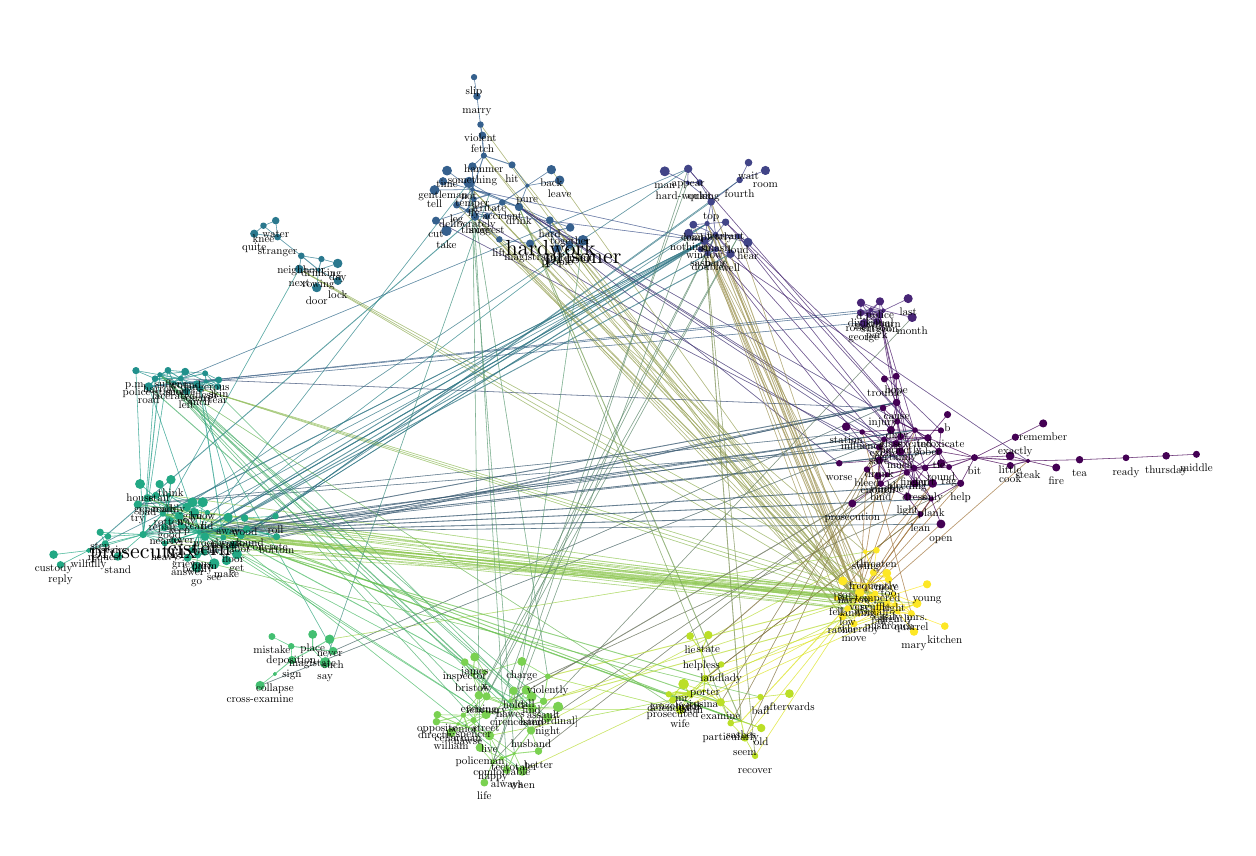
\begin{tikzpicture}[x=1pt,y=1pt]
\definecolor{fillColor}{RGB}{255,255,255}
\path[use as bounding box,fill=fillColor,fill opacity=0.00] (0,0) rectangle (433.62,289.08);
\begin{scope}
\path[clip] (  0.00,  0.00) rectangle (433.62,289.08);
\definecolor{drawColor}{RGB}{43,131,136}

\path[draw=drawColor,draw opacity=0.50,line width= 0.2pt,line join=round,line cap=round] ( 61.95,106.77) -- (159.49,233.17);
\definecolor{drawColor}{RGB}{87,152,111}

\path[draw=drawColor,draw opacity=0.50,line width= 0.2pt,line join=round,line cap=round] (175.85, 26.78) -- (159.49,233.17);
\definecolor{drawColor}{RGB}{53,96,141}

\path[draw=drawColor,draw opacity=0.50,line width= 0.2pt,line join=round,line cap=round] (166.80,228.86) -- (159.49,233.17);
\definecolor{drawColor}{RGB}{60,143,127}

\path[draw=drawColor,draw opacity=0.50,line width= 0.2pt,line join=round,line cap=round] (166.80,228.86) -- (107.51, 59.64);
\definecolor{drawColor}{RGB}{67,191,113}

\path[draw=drawColor,draw opacity=0.50,line width= 0.2pt,line join=round,line cap=round] (102.96, 64.54) -- (107.51, 59.64);
\definecolor{drawColor}{RGB}{43,131,136}

\path[draw=drawColor,draw opacity=0.50,line width= 0.2pt,line join=round,line cap=round] ( 61.95,106.77) -- (200.65,212.21);
\definecolor{drawColor}{RGB}{87,152,111}

\path[draw=drawColor,draw opacity=0.50,line width= 0.2pt,line join=round,line cap=round] (176.31, 43.01) -- (200.65,212.21);
\definecolor{drawColor}{RGB}{53,96,141}

\path[draw=drawColor,draw opacity=0.50,line width= 0.2pt,line join=round,line cap=round] (188.94,215.26) -- (200.65,212.21);
\definecolor{drawColor}{RGB}{34,168,132}

\path[draw=drawColor,draw opacity=0.50,line width= 0.2pt,line join=round,line cap=round] ( 61.95,106.77) -- ( 61.07, 94.19);

\path[draw=drawColor,draw opacity=0.50,line width= 0.2pt,line join=round,line cap=round] ( 61.95,106.77) -- ( 67.39, 95.41);
\definecolor{drawColor}{RGB}{187,223,39}

\path[draw=drawColor,draw opacity=0.50,line width= 0.2pt,line join=round,line cap=round] (238.98, 48.62) -- (237.01, 51.89);

\path[draw=drawColor,draw opacity=0.50,line width= 0.2pt,line join=round,line cap=round] (239.70, 47.52) -- (237.01, 51.89);

\path[draw=drawColor,draw opacity=0.50,line width= 0.2pt,line join=round,line cap=round] (244.31, 49.49) -- (237.01, 51.89);

\path[draw=drawColor,draw opacity=0.50,line width= 0.3pt,line join=round,line cap=round] (234.38, 49.07) -- (237.01, 51.89);
\definecolor{drawColor}{RGB}{53,96,141}

\path[draw=drawColor,draw opacity=0.50,line width= 0.2pt,line join=round,line cap=round] (158.94,223.05) -- (151.32,215.67);
\definecolor{drawColor}{RGB}{122,209,81}

\path[draw=drawColor,draw opacity=0.50,line width= 0.2pt,line join=round,line cap=round] (176.31, 43.01) -- (191.66, 43.67);
\definecolor{drawColor}{RGB}{34,168,132}

\path[draw=drawColor,draw opacity=0.50,line width= 0.2pt,line join=round,line cap=round] ( 61.95,106.77) -- ( 63.26,117.59);

\path[draw=drawColor,draw opacity=0.50,line width= 0.2pt,line join=round,line cap=round] ( 50.87,115.41) -- ( 63.26,117.59);

\path[draw=drawColor,draw opacity=0.50,line width= 0.2pt,line join=round,line cap=round] ( 64.91,113.87) -- ( 59.53,117.54);

\path[draw=drawColor,draw opacity=0.50,line width= 0.2pt,line join=round,line cap=round] ( 50.99,120.11) -- ( 59.53,117.54);

\path[draw=drawColor,draw opacity=0.50,line width= 0.2pt,line join=round,line cap=round] ( 61.95,106.77) -- ( 59.53,117.54);

\path[draw=drawColor,draw opacity=0.50,line width= 0.2pt,line join=round,line cap=round] ( 50.87,115.41) -- ( 59.53,117.54);
\definecolor{drawColor}{RGB}{187,220,59}

\path[draw=drawColor,draw opacity=0.50,line width= 0.2pt,line join=round,line cap=round] (313.01, 84.20) -- (178.74, 20.55);
\definecolor{drawColor}{RGB}{122,209,81}

\path[draw=drawColor,draw opacity=0.50,line width= 0.2pt,line join=round,line cap=round] (171.33, 25.08) -- (178.74, 20.55);
\definecolor{drawColor}{RGB}{78,188,106}

\path[draw=drawColor,draw opacity=0.50,line width= 0.2pt,line join=round,line cap=round] ( 68.71,107.91) -- (178.74, 20.55);
\definecolor{drawColor}{RGB}{122,209,81}

\path[draw=drawColor,draw opacity=0.50,line width= 0.2pt,line join=round,line cap=round] (175.85, 26.78) -- (178.74, 20.55);
\definecolor{drawColor}{RGB}{65,68,135}

\path[draw=drawColor,draw opacity=0.50,line width= 0.2pt,line join=round,line cap=round] (238.49,233.08) -- (230.22,237.16);
\definecolor{drawColor}{RGB}{143,199,84}

\path[draw=drawColor,draw opacity=0.50,line width= 0.2pt,line join=round,line cap=round] (313.01, 84.20) -- ( 75.62, 98.79);
\definecolor{drawColor}{RGB}{34,168,132}

\path[draw=drawColor,draw opacity=0.50,line width= 0.2pt,line join=round,line cap=round] ( 61.95,106.77) -- ( 75.62, 98.79);
\definecolor{drawColor}{RGB}{122,209,81}

\path[draw=drawColor,draw opacity=0.50,line width= 0.2pt,line join=round,line cap=round] (174.46, 45.94) -- (182.11, 47.37);

\path[draw=drawColor,draw opacity=0.50,line width= 0.2pt,line join=round,line cap=round] (176.31, 43.01) -- (182.11, 47.37);
\definecolor{drawColor}{RGB}{34,168,132}

\path[draw=drawColor,draw opacity=0.50,line width= 0.2pt,line join=round,line cap=round] ( 50.87,115.41) -- ( 40.60,124.20);
\definecolor{drawColor}{RGB}{53,96,141}

\path[draw=drawColor,draw opacity=0.50,line width= 0.2pt,line join=round,line cap=round] (160.72,230.59) -- (147.03,230.41);

\path[draw=drawColor,draw opacity=0.50,line width= 0.2pt,line join=round,line cap=round] (160.72,230.59) -- (151.54,237.41);
\definecolor{drawColor}{RGB}{34,168,132}

\path[draw=drawColor,draw opacity=0.50,line width= 0.2pt,line join=round,line cap=round] ( 61.95,106.77) -- ( 71.85, 96.57);
\definecolor{drawColor}{RGB}{77,176,110}

\path[draw=drawColor,draw opacity=0.50,line width= 0.2pt,line join=round,line cap=round] ( 47.79,163.64) -- (166.84, 33.29);
\definecolor{drawColor}{RGB}{122,209,81}

\path[draw=drawColor,draw opacity=0.50,line width= 0.2pt,line join=round,line cap=round] (168.10, 23.78) -- (166.84, 33.29);

\path[draw=drawColor,draw opacity=0.50,line width= 0.2pt,line join=round,line cap=round] (157.44, 40.67) -- (166.84, 33.29);
\definecolor{drawColor}{RGB}{154,216,60}

\path[draw=drawColor,draw opacity=0.50,line width= 0.2pt,line join=round,line cap=round] (239.70, 47.52) -- (166.84, 33.29);
\definecolor{drawColor}{RGB}{122,209,81}

\path[draw=drawColor,draw opacity=0.50,line width= 0.2pt,line join=round,line cap=round] (171.33, 25.08) -- (166.84, 33.29);
\definecolor{drawColor}{RGB}{93,138,108}

\path[draw=drawColor,draw opacity=0.50,line width= 0.2pt,line join=round,line cap=round] (238.49,233.08) -- (166.84, 33.29);
\definecolor{drawColor}{RGB}{122,209,81}

\path[draw=drawColor,draw opacity=0.50,line width= 0.2pt,line join=round,line cap=round] (155.52, 37.48) -- (166.84, 33.29);

\path[draw=drawColor,draw opacity=0.50,line width= 0.2pt,line join=round,line cap=round] (176.31, 43.01) -- (166.84, 33.29);

\path[draw=drawColor,draw opacity=0.50,line width= 0.2pt,line join=round,line cap=round] (175.85, 26.78) -- (166.84, 33.29);

\path[draw=drawColor,draw opacity=0.50,line width= 0.3pt,line join=round,line cap=round] (159.07, 36.23) -- (166.84, 33.29);
\definecolor{drawColor}{RGB}{42,120,142}

\path[draw=drawColor,draw opacity=0.50,line width= 0.2pt,line join=round,line cap=round] (106.16,205.48) -- (112.04,203.90);

\path[draw=drawColor,draw opacity=0.50,line width= 0.2pt,line join=round,line cap=round] (105.12,201.59) -- (112.04,203.90);
\definecolor{drawColor}{RGB}{160,211,74}

\path[draw=drawColor,draw opacity=0.50,line width= 0.2pt,line join=round,line cap=round] (306.72,100.24) -- (109.13, 68.10);
\definecolor{drawColor}{RGB}{67,191,113}

\path[draw=drawColor,draw opacity=0.50,line width= 0.3pt,line join=round,line cap=round] (102.96, 64.54) -- (109.13, 68.10);
\definecolor{drawColor}{RGB}{42,120,142}

\path[draw=drawColor,draw opacity=0.50,line width= 0.2pt,line join=round,line cap=round] (105.12,201.59) -- (104.45,195.15);
\definecolor{drawColor}{RGB}{122,209,81}

\path[draw=drawColor,draw opacity=0.50,line width= 0.2pt,line join=round,line cap=round] (161.13, 38.87) -- (153.04, 34.39);

\path[draw=drawColor,draw opacity=0.50,line width= 0.2pt,line join=round,line cap=round] (155.52, 37.48) -- (153.04, 34.39);

\path[draw=drawColor,draw opacity=0.50,line width= 0.3pt,line join=round,line cap=round] (159.07, 36.23) -- (153.04, 34.39);
\definecolor{drawColor}{RGB}{53,96,141}

\path[draw=drawColor,draw opacity=0.50,line width= 0.2pt,line join=round,line cap=round] (180.53,232.00) -- (192.24,233.97);
\definecolor{drawColor}{RGB}{160,116,60}

\path[draw=drawColor,draw opacity=0.50,line width= 0.2pt,line join=round,line cap=round] (303.26,129.44) -- (300.64, 84.88);
\definecolor{drawColor}{RGB}{253,231,37}

\path[draw=drawColor,draw opacity=0.50,line width= 0.2pt,line join=round,line cap=round] (296.23, 79.14) -- (300.64, 84.88);
\definecolor{drawColor}{RGB}{143,199,84}

\path[draw=drawColor,draw opacity=0.50,line width= 0.2pt,line join=round,line cap=round] ( 48.83,113.44) -- (300.64, 84.88);
\definecolor{drawColor}{RGB}{253,231,37}

\path[draw=drawColor,draw opacity=0.50,line width= 0.2pt,line join=round,line cap=round] (299.86, 82.50) -- (300.64, 84.88);
\definecolor{drawColor}{RGB}{160,116,60}

\path[draw=drawColor,draw opacity=0.50,line width= 0.2pt,line join=round,line cap=round] (320.64,143.66) -- (300.64, 84.88);

\path[draw=drawColor,draw opacity=0.50,line width= 0.2pt,line join=round,line cap=round] (309.40,140.32) -- (300.64, 84.88);
\definecolor{drawColor}{RGB}{159,149,86}

\path[draw=drawColor,draw opacity=0.50,line width= 0.2pt,line join=round,line cap=round] (256.81,213.70) -- (300.64, 84.88);

\path[draw=drawColor,draw opacity=0.50,line width= 0.2pt,line join=round,line cap=round] (248.59,214.36) -- (300.64, 84.88);
\definecolor{drawColor}{RGB}{253,231,37}

\path[draw=drawColor,draw opacity=0.50,line width= 0.2pt,line join=round,line cap=round] (313.01, 84.20) -- (300.64, 84.88);
\definecolor{drawColor}{RGB}{143,199,84}

\path[draw=drawColor,draw opacity=0.50,line width= 0.2pt,line join=round,line cap=round] ( 50.99,120.11) -- (300.64, 84.88);

\path[draw=drawColor,draw opacity=0.50,line width= 0.3pt,line join=round,line cap=round] ( 50.87,115.41) -- (300.64, 84.88);
\definecolor{drawColor}{RGB}{220,227,38}

\path[draw=drawColor,draw opacity=0.50,line width= 0.3pt,line join=round,line cap=round] (257.82, 38.47) -- (300.64, 84.88);
\definecolor{drawColor}{RGB}{253,231,37}

\path[draw=drawColor,draw opacity=0.50,line width= 0.3pt,line join=round,line cap=round] (303.30, 88.07) -- (300.64, 84.88);
\definecolor{drawColor}{RGB}{122,209,81}

\path[draw=drawColor,draw opacity=0.50,line width= 0.2pt,line join=round,line cap=round] (174.46, 45.94) -- (180.17, 49.73);

\path[draw=drawColor,draw opacity=0.50,line width= 0.2pt,line join=round,line cap=round] (176.31, 43.01) -- (180.17, 49.73);
\definecolor{drawColor}{RGB}{153,163,89}

\path[draw=drawColor,draw opacity=0.50,line width= 0.2pt,line join=round,line cap=round] (299.86, 82.50) -- (189.23,237.76);
\definecolor{drawColor}{RGB}{53,96,141}

\path[draw=drawColor,draw opacity=0.50,line width= 0.2pt,line join=round,line cap=round] (180.53,232.00) -- (189.23,237.76);
\definecolor{drawColor}{RGB}{34,168,132}

\path[draw=drawColor,draw opacity=0.50,line width= 0.2pt,line join=round,line cap=round] ( 50.99,120.11) -- ( 51.77,125.75);

\path[draw=drawColor,draw opacity=0.50,line width= 0.2pt,line join=round,line cap=round] ( 50.87,115.41) -- ( 51.77,125.75);

\path[draw=drawColor,draw opacity=0.50,line width= 0.2pt,line join=round,line cap=round] ( 61.95,106.77) -- ( 60.24,113.86);

\path[draw=drawColor,draw opacity=0.50,line width= 0.2pt,line join=round,line cap=round] ( 50.87,115.41) -- ( 60.24,113.86);
\definecolor{drawColor}{RGB}{77,176,110}

\path[draw=drawColor,draw opacity=0.50,line width= 0.2pt,line join=round,line cap=round] ( 64.50,161.20) -- (182.28, 43.20);
\definecolor{drawColor}{RGB}{78,188,106}

\path[draw=drawColor,draw opacity=0.50,line width= 0.2pt,line join=round,line cap=round] ( 61.95,106.77) -- (182.28, 43.20);
\definecolor{drawColor}{RGB}{122,209,81}

\path[draw=drawColor,draw opacity=0.50,line width= 0.2pt,line join=round,line cap=round] (174.46, 45.94) -- (182.28, 43.20);
\definecolor{drawColor}{RGB}{77,176,110}

\path[draw=drawColor,draw opacity=0.50,line width= 0.2pt,line join=round,line cap=round] ( 52.79,160.87) -- (182.28, 43.20);
\definecolor{drawColor}{RGB}{122,209,81}

\path[draw=drawColor,draw opacity=0.50,line width= 0.2pt,line join=round,line cap=round] (176.31, 43.01) -- (182.28, 43.20);
\definecolor{drawColor}{RGB}{65,68,135}

\path[draw=drawColor,draw opacity=0.50,line width= 0.2pt,line join=round,line cap=round] (256.81,213.70) -- (260.26,211.50);

\path[draw=drawColor,draw opacity=0.50,line width= 0.2pt,line join=round,line cap=round] (248.59,214.36) -- (260.26,211.50);
\definecolor{drawColor}{RGB}{67,96,98}

\path[draw=drawColor,draw opacity=0.50,line width= 0.2pt,line join=round,line cap=round] (309.40,140.32) -- ( 84.00, 51.36);
\definecolor{drawColor}{RGB}{67,191,113}

\path[draw=drawColor,draw opacity=0.50,line width= 0.2pt,line join=round,line cap=round] ( 89.33, 55.55) -- ( 84.00, 51.36);
\definecolor{drawColor}{RGB}{77,176,110}

\path[draw=drawColor,draw opacity=0.50,line width= 0.2pt,line join=round,line cap=round] ( 47.79,163.64) -- (165.64, 40.88);
\definecolor{drawColor}{RGB}{122,209,81}

\path[draw=drawColor,draw opacity=0.50,line width= 0.2pt,line join=round,line cap=round] (157.44, 40.67) -- (165.64, 40.88);
\definecolor{drawColor}{RGB}{78,188,106}

\path[draw=drawColor,draw opacity=0.50,line width= 0.2pt,line join=round,line cap=round] ( 61.95,106.77) -- (165.64, 40.88);
\definecolor{drawColor}{RGB}{122,209,81}

\path[draw=drawColor,draw opacity=0.50,line width= 0.2pt,line join=round,line cap=round] (174.46, 45.94) -- (165.64, 40.88);
\definecolor{drawColor}{RGB}{78,188,106}

\path[draw=drawColor,draw opacity=0.50,line width= 0.2pt,line join=round,line cap=round] ( 50.87,115.41) -- (165.64, 40.88);
\definecolor{drawColor}{RGB}{122,209,81}

\path[draw=drawColor,draw opacity=0.50,line width= 0.2pt,line join=round,line cap=round] (155.52, 37.48) -- (165.64, 40.88);

\path[draw=drawColor,draw opacity=0.50,line width= 0.3pt,line join=round,line cap=round] (176.31, 43.01) -- (165.64, 40.88);

\path[draw=drawColor,draw opacity=0.50,line width= 0.3pt,line join=round,line cap=round] (159.07, 36.23) -- (165.64, 40.88);
\definecolor{drawColor}{RGB}{97,123,99}

\path[draw=drawColor,draw opacity=0.50,line width= 0.2pt,line join=round,line cap=round] (168.10, 23.78) -- (319.61,184.37);
\definecolor{drawColor}{RGB}{72,37,118}

\path[draw=drawColor,draw opacity=0.50,line width= 0.2pt,line join=round,line cap=round] (309.21,186.86) -- (319.61,184.37);
\definecolor{drawColor}{RGB}{34,168,132}

\path[draw=drawColor,draw opacity=0.50,line width= 0.2pt,line join=round,line cap=round] ( 61.95,106.77) -- ( 72.42,112.15);

\path[draw=drawColor,draw opacity=0.50,line width= 0.2pt,line join=round,line cap=round] ( 68.71,107.91) -- ( 72.42,112.15);
\definecolor{drawColor}{RGB}{77,176,110}

\path[draw=drawColor,draw opacity=0.50,line width= 0.2pt,line join=round,line cap=round] ( 47.79,163.64) -- (187.92, 39.77);
\definecolor{drawColor}{RGB}{122,209,81}

\path[draw=drawColor,draw opacity=0.50,line width= 0.2pt,line join=round,line cap=round] (176.31, 43.01) -- (187.92, 39.77);
\definecolor{drawColor}{RGB}{65,68,135}

\path[draw=drawColor,draw opacity=0.50,line width= 0.2pt,line join=round,line cap=round] (257.26,234.03) -- (266.59,237.48);
\definecolor{drawColor}{RGB}{253,231,37}

\path[draw=drawColor,draw opacity=0.50,line width= 0.2pt,line join=round,line cap=round] (299.86, 82.50) -- (294.55, 89.16);

\path[draw=drawColor,draw opacity=0.50,line width= 0.2pt,line join=round,line cap=round] (298.82, 87.10) -- (294.55, 89.16);

\path[draw=drawColor,draw opacity=0.50,line width= 0.3pt,line join=round,line cap=round] (303.30, 88.07) -- (294.55, 89.16);
\definecolor{drawColor}{RGB}{72,37,118}

\path[draw=drawColor,draw opacity=0.50,line width= 0.2pt,line join=round,line cap=round] (309.21,186.86) -- (318.17,191.17);
\definecolor{drawColor}{RGB}{65,68,135}

\path[draw=drawColor,draw opacity=0.50,line width= 0.2pt,line join=round,line cap=round] (248.59,214.36) -- (238.81,214.79);

\path[draw=drawColor,draw opacity=0.50,line width= 0.2pt,line join=round,line cap=round] (245.51,218.29) -- (238.81,214.79);
\definecolor{drawColor}{RGB}{122,209,81}

\path[draw=drawColor,draw opacity=0.50,line width= 0.2pt,line join=round,line cap=round] (187.93, 54.67) -- (178.57, 60.06);

\path[draw=drawColor,draw opacity=0.50,line width= 0.2pt,line join=round,line cap=round] (165.06, 56.20) -- (178.57, 60.06);
\definecolor{drawColor}{RGB}{220,227,38}

\path[draw=drawColor,draw opacity=0.50,line width= 0.2pt,line join=round,line cap=round] (244.77, 53.93) -- (321.36, 81.01);

\path[draw=drawColor,draw opacity=0.50,line width= 0.2pt,line join=round,line cap=round] (250.61, 58.99) -- (321.36, 81.01);
\definecolor{drawColor}{RGB}{253,231,37}

\path[draw=drawColor,draw opacity=0.50,line width= 0.2pt,line join=round,line cap=round] (313.49, 80.53) -- (321.36, 81.01);

\path[draw=drawColor,draw opacity=0.50,line width= 0.2pt,line join=round,line cap=round] (314.41, 77.97) -- (321.36, 81.01);

\path[draw=drawColor,draw opacity=0.50,line width= 0.2pt,line join=round,line cap=round] (313.01, 84.20) -- (321.36, 81.01);
\definecolor{drawColor}{RGB}{143,199,84}

\path[draw=drawColor,draw opacity=0.50,line width= 0.2pt,line join=round,line cap=round] ( 61.95,106.77) -- (321.36, 81.01);
\definecolor{drawColor}{RGB}{122,209,81}

\path[draw=drawColor,draw opacity=0.50,line width= 0.2pt,line join=round,line cap=round] (165.06, 56.20) -- (161.53, 61.66);

\path[draw=drawColor,draw opacity=0.50,line width= 0.3pt,line join=round,line cap=round] (160.86, 55.27) -- (161.53, 61.66);
\definecolor{drawColor}{RGB}{160,116,60}

\path[draw=drawColor,draw opacity=0.50,line width= 0.2pt,line join=round,line cap=round] (299.86, 82.50) -- (330.02,109.73);
\definecolor{drawColor}{RGB}{68,1,84}

\path[draw=drawColor,draw opacity=0.50,line width= 0.2pt,line join=round,line cap=round] (326.52,118.77) -- (330.02,109.73);
\definecolor{drawColor}{RGB}{51,84,108}

\path[draw=drawColor,draw opacity=0.50,line width= 0.2pt,line join=round,line cap=round] ( 61.95,106.77) -- (330.02,109.73);
\definecolor{drawColor}{RGB}{67,191,113}

\path[draw=drawColor,draw opacity=0.50,line width= 0.3pt,line join=round,line cap=round] (102.96, 64.54) -- (102.98, 69.84);
\definecolor{drawColor}{RGB}{154,216,60}

\path[draw=drawColor,draw opacity=0.50,line width= 0.2pt,line join=round,line cap=round] (187.93, 54.67) -- (235.77, 42.54);
\definecolor{drawColor}{RGB}{187,223,39}

\path[draw=drawColor,draw opacity=0.50,line width= 0.2pt,line join=round,line cap=round] (238.98, 48.62) -- (235.77, 42.54);
\definecolor{drawColor}{RGB}{220,227,38}

\path[draw=drawColor,draw opacity=0.50,line width= 0.2pt,line join=round,line cap=round] (314.41, 77.97) -- (235.77, 42.54);
\definecolor{drawColor}{RGB}{110,183,89}

\path[draw=drawColor,draw opacity=0.50,line width= 0.2pt,line join=round,line cap=round] ( 47.79,163.64) -- (235.77, 42.54);
\definecolor{drawColor}{RGB}{187,223,39}

\path[draw=drawColor,draw opacity=0.50,line width= 0.2pt,line join=round,line cap=round] (239.70, 47.52) -- (235.77, 42.54);
\definecolor{drawColor}{RGB}{220,227,38}

\path[draw=drawColor,draw opacity=0.50,line width= 0.2pt,line join=round,line cap=round] (300.49, 76.88) -- (235.77, 42.54);
\definecolor{drawColor}{RGB}{154,216,60}

\path[draw=drawColor,draw opacity=0.50,line width= 0.2pt,line join=round,line cap=round] (176.31, 43.01) -- (235.77, 42.54);
\definecolor{drawColor}{RGB}{68,1,84}

\path[draw=drawColor,draw opacity=0.50,line width= 0.2pt,line join=round,line cap=round] (324.32,130.01) -- (326.99,124.41);

\path[draw=drawColor,draw opacity=0.50,line width= 0.2pt,line join=round,line cap=round] (320.28,129.94) -- (326.99,124.41);
\definecolor{drawColor}{RGB}{160,116,60}

\path[draw=drawColor,draw opacity=0.50,line width= 0.2pt,line join=round,line cap=round] (299.86, 82.50) -- (326.99,124.41);

\path[draw=drawColor,draw opacity=0.50,line width= 0.2pt,line join=round,line cap=round] (292.23, 82.91) -- (326.99,124.41);
\definecolor{drawColor}{RGB}{34,168,132}

\path[draw=drawColor,draw opacity=0.50,line width= 0.2pt,line join=round,line cap=round] ( 48.83,113.44) -- ( 54.80,112.68);

\path[draw=drawColor,draw opacity=0.50,line width= 0.2pt,line join=round,line cap=round] ( 61.95,106.77) -- ( 54.80,112.68);

\path[draw=drawColor,draw opacity=0.50,line width= 0.2pt,line join=round,line cap=round] ( 50.87,115.41) -- ( 54.80,112.68);
\definecolor{drawColor}{RGB}{253,231,37}

\path[draw=drawColor,draw opacity=0.50,line width= 0.2pt,line join=round,line cap=round] (305.58, 92.21) -- (310.44, 91.95);

\path[draw=drawColor,draw opacity=0.50,line width= 0.2pt,line join=round,line cap=round] (313.01, 84.20) -- (310.44, 91.95);

\path[draw=drawColor,draw opacity=0.50,line width= 0.3pt,line join=round,line cap=round] (303.30, 88.07) -- (310.44, 91.95);
\definecolor{drawColor}{RGB}{72,37,118}

\path[draw=drawColor,draw opacity=0.50,line width= 0.2pt,line join=round,line cap=round] (303.87,185.53) -- (302.12,182.18);

\path[draw=drawColor,draw opacity=0.50,line width= 0.2pt,line join=round,line cap=round] (304.68,187.22) -- (302.12,182.18);

\path[draw=drawColor,draw opacity=0.50,line width= 0.2pt,line join=round,line cap=round] (309.21,186.86) -- (302.12,182.18);
\definecolor{drawColor}{RGB}{187,223,39}

\path[draw=drawColor,draw opacity=0.50,line width= 0.2pt,line join=round,line cap=round] (264.80, 47.22) -- (275.26, 48.43);
\definecolor{drawColor}{RGB}{253,231,37}

\path[draw=drawColor,draw opacity=0.50,line width= 0.2pt,line join=round,line cap=round] (306.26, 84.62) -- (304.86, 82.97);
\definecolor{drawColor}{RGB}{143,199,84}

\path[draw=drawColor,draw opacity=0.50,line width= 0.2pt,line join=round,line cap=round] ( 49.54,102.74) -- (304.86, 82.97);

\path[draw=drawColor,draw opacity=0.50,line width= 0.2pt,line join=round,line cap=round] ( 52.76,103.83) -- (304.86, 82.97);
\definecolor{drawColor}{RGB}{253,231,37}

\path[draw=drawColor,draw opacity=0.50,line width= 0.2pt,line join=round,line cap=round] (299.86, 82.50) -- (304.86, 82.97);

\path[draw=drawColor,draw opacity=0.50,line width= 0.2pt,line join=round,line cap=round] (310.74, 80.98) -- (304.86, 82.97);

\path[draw=drawColor,draw opacity=0.50,line width= 0.2pt,line join=round,line cap=round] (313.49, 80.53) -- (304.86, 82.97);

\path[draw=drawColor,draw opacity=0.50,line width= 0.2pt,line join=round,line cap=round] (314.41, 77.97) -- (304.86, 82.97);

\path[draw=drawColor,draw opacity=0.50,line width= 0.2pt,line join=round,line cap=round] (298.82, 87.10) -- (304.86, 82.97);
\definecolor{drawColor}{RGB}{159,149,86}

\path[draw=drawColor,draw opacity=0.50,line width= 0.2pt,line join=round,line cap=round] (248.59,214.36) -- (304.86, 82.97);

\path[draw=drawColor,draw opacity=0.50,line width= 0.2pt,line join=round,line cap=round] (245.51,218.29) -- (304.86, 82.97);
\definecolor{drawColor}{RGB}{253,231,37}

\path[draw=drawColor,draw opacity=0.50,line width= 0.2pt,line join=round,line cap=round] (313.01, 84.20) -- (304.86, 82.97);

\path[draw=drawColor,draw opacity=0.50,line width= 0.2pt,line join=round,line cap=round] (292.23, 82.91) -- (304.86, 82.97);
\definecolor{drawColor}{RGB}{160,116,60}

\path[draw=drawColor,draw opacity=0.50,line width= 0.2pt,line join=round,line cap=round] (361.49,132.53) -- (304.86, 82.97);
\definecolor{drawColor}{RGB}{143,199,84}

\path[draw=drawColor,draw opacity=0.50,line width= 0.2pt,line join=round,line cap=round] ( 61.95,106.77) -- (304.86, 82.97);
\definecolor{drawColor}{RGB}{253,231,37}

\path[draw=drawColor,draw opacity=0.50,line width= 0.3pt,line join=round,line cap=round] (303.30, 88.07) -- (304.86, 82.97);
\definecolor{drawColor}{RGB}{52,90,129}

\path[draw=drawColor,draw opacity=0.50,line width= 0.2pt,line join=round,line cap=round] (306.81,182.87) -- ( 43.74,159.37);
\definecolor{drawColor}{RGB}{33,144,140}

\path[draw=drawColor,draw opacity=0.50,line width= 0.2pt,line join=round,line cap=round] ( 46.04,162.24) -- ( 43.74,159.37);

\path[draw=drawColor,draw opacity=0.50,line width= 0.3pt,line join=round,line cap=round] ( 47.79,163.64) -- ( 43.74,159.37);
\definecolor{drawColor}{RGB}{52,90,129}

\path[draw=drawColor,draw opacity=0.50,line width= 0.2pt,line join=round,line cap=round] (304.68,187.22) -- ( 43.74,159.37);

\path[draw=drawColor,draw opacity=0.50,line width= 0.2pt,line join=round,line cap=round] (309.21,186.86) -- ( 43.74,159.37);
\definecolor{drawColor}{RGB}{33,156,136}

\path[draw=drawColor,draw opacity=0.50,line width= 0.2pt,line join=round,line cap=round] ( 61.95,106.77) -- ( 43.74,159.37);
\definecolor{drawColor}{RGB}{33,144,140}

\path[draw=drawColor,draw opacity=0.50,line width= 0.2pt,line join=round,line cap=round] ( 52.79,160.87) -- ( 43.74,159.37);
\definecolor{drawColor}{RGB}{77,176,110}

\path[draw=drawColor,draw opacity=0.50,line width= 0.3pt,line join=round,line cap=round] (176.31, 43.01) -- ( 43.74,159.37);
\definecolor{drawColor}{RGB}{34,168,132}

\path[draw=drawColor,draw opacity=0.50,line width= 0.2pt,line join=round,line cap=round] ( 48.83,113.44) -- ( 51.23,110.83);
\definecolor{drawColor}{RGB}{143,199,84}

\path[draw=drawColor,draw opacity=0.50,line width= 0.2pt,line join=round,line cap=round] (313.01, 84.20) -- ( 51.23,110.83);
\definecolor{drawColor}{RGB}{34,168,132}

\path[draw=drawColor,draw opacity=0.50,line width= 0.2pt,line join=round,line cap=round] ( 61.95,106.77) -- ( 51.23,110.83);

\path[draw=drawColor,draw opacity=0.50,line width= 0.2pt,line join=round,line cap=round] ( 50.87,115.41) -- ( 51.23,110.83);
\definecolor{drawColor}{RGB}{42,120,142}

\path[draw=drawColor,draw opacity=0.50,line width= 0.2pt,line join=round,line cap=round] ( 98.87,206.63) -- ( 98.12,201.84);
\definecolor{drawColor}{RGB}{38,144,137}

\path[draw=drawColor,draw opacity=0.50,line width= 0.2pt,line join=round,line cap=round] ( 48.83,113.44) -- ( 98.12,201.84);
\definecolor{drawColor}{RGB}{147,175,89}

\path[draw=drawColor,draw opacity=0.50,line width= 0.2pt,line join=round,line cap=round] (299.86, 82.50) -- ( 98.12,201.84);

\path[draw=drawColor,draw opacity=0.50,line width= 0.2pt,line join=round,line cap=round] (314.41, 77.97) -- ( 98.12,201.84);

\path[draw=drawColor,draw opacity=0.50,line width= 0.2pt,line join=round,line cap=round] (313.01, 84.20) -- ( 98.12,201.84);
\definecolor{drawColor}{RGB}{42,120,142}

\path[draw=drawColor,draw opacity=0.50,line width= 0.2pt,line join=round,line cap=round] (105.12,201.59) -- ( 98.12,201.84);
\definecolor{drawColor}{RGB}{68,1,84}

\path[draw=drawColor,draw opacity=0.50,line width= 0.2pt,line join=round,line cap=round] (342.14,133.73) -- (355.00,134.34);

\path[draw=drawColor,draw opacity=0.50,line width= 0.2pt,line join=round,line cap=round] (361.49,132.53) -- (355.00,134.34);
\definecolor{drawColor}{RGB}{122,209,81}

\path[draw=drawColor,draw opacity=0.50,line width= 0.2pt,line join=round,line cap=round] (161.13, 38.87) -- (163.44, 28.93);

\path[draw=drawColor,draw opacity=0.50,line width= 0.2pt,line join=round,line cap=round] (168.10, 23.78) -- (163.44, 28.93);
\definecolor{drawColor}{RGB}{87,152,111}

\path[draw=drawColor,draw opacity=0.50,line width= 0.2pt,line join=round,line cap=round] (160.72,230.59) -- (163.44, 28.93);
\definecolor{drawColor}{RGB}{122,209,81}

\path[draw=drawColor,draw opacity=0.50,line width= 0.2pt,line join=round,line cap=round] (171.33, 25.08) -- (163.44, 28.93);
\definecolor{drawColor}{RGB}{95,105,82}

\path[draw=drawColor,draw opacity=0.50,line width= 0.2pt,line join=round,line cap=round] (326.52,118.77) -- (175.56, 49.46);
\definecolor{drawColor}{RGB}{122,209,81}

\path[draw=drawColor,draw opacity=0.50,line width= 0.3pt,line join=round,line cap=round] (174.46, 45.94) -- (175.56, 49.46);

\path[draw=drawColor,draw opacity=0.50,line width= 0.2pt,line join=round,line cap=round] (176.31, 43.01) -- (175.56, 49.46);
\definecolor{drawColor}{RGB}{34,168,132}

\path[draw=drawColor,draw opacity=0.50,line width= 0.2pt,line join=round,line cap=round] ( 22.00,100.16) -- (  9.36, 98.68);

\path[draw=drawColor,draw opacity=0.50,line width= 0.2pt,line join=round,line cap=round] ( 64.91,113.87) -- ( 57.44,115.90);

\path[draw=drawColor,draw opacity=0.50,line width= 0.3pt,line join=round,line cap=round] ( 50.99,120.11) -- ( 57.44,115.90);

\path[draw=drawColor,draw opacity=0.50,line width= 0.2pt,line join=round,line cap=round] ( 61.95,106.77) -- ( 57.44,115.90);

\path[draw=drawColor,draw opacity=0.50,line width= 0.2pt,line join=round,line cap=round] ( 50.87,115.41) -- ( 57.44,115.90);
\definecolor{drawColor}{RGB}{122,209,81}

\path[draw=drawColor,draw opacity=0.50,line width= 0.2pt,line join=round,line cap=round] (161.13, 38.87) -- (163.06, 47.84);
\definecolor{drawColor}{RGB}{93,138,108}

\path[draw=drawColor,draw opacity=0.50,line width= 0.2pt,line join=round,line cap=round] (256.81,213.70) -- (163.06, 47.84);

\path[draw=drawColor,draw opacity=0.50,line width= 0.2pt,line join=round,line cap=round] (248.59,214.36) -- (163.06, 47.84);
\definecolor{drawColor}{RGB}{122,209,81}

\path[draw=drawColor,draw opacity=0.50,line width= 0.2pt,line join=round,line cap=round] (157.44, 40.67) -- (163.06, 47.84);

\path[draw=drawColor,draw opacity=0.50,line width= 0.2pt,line join=round,line cap=round] (165.06, 56.20) -- (163.06, 47.84);

\path[draw=drawColor,draw opacity=0.50,line width= 0.2pt,line join=round,line cap=round] (160.86, 55.27) -- (163.06, 47.84);

\path[draw=drawColor,draw opacity=0.50,line width= 0.2pt,line join=round,line cap=round] (176.31, 43.01) -- (163.06, 47.84);
\definecolor{drawColor}{RGB}{68,1,84}

\path[draw=drawColor,draw opacity=0.50,line width= 0.2pt,line join=round,line cap=round] (309.40,140.32) -- (295.77,144.91);
\definecolor{drawColor}{RGB}{34,168,132}

\path[draw=drawColor,draw opacity=0.50,line width= 0.2pt,line join=round,line cap=round] ( 41.71,105.93) -- ( 32.58, 98.00);
\definecolor{drawColor}{RGB}{49,118,133}

\path[draw=drawColor,draw opacity=0.50,line width= 0.2pt,line join=round,line cap=round] ( 77.03,105.69) -- (244.56,212.07);

\path[draw=drawColor,draw opacity=0.50,line width= 0.2pt,line join=round,line cap=round] ( 41.71,105.93) -- (244.56,212.07);
\definecolor{drawColor}{RGB}{159,149,86}

\path[draw=drawColor,draw opacity=0.50,line width= 0.2pt,line join=round,line cap=round] (306.57, 77.89) -- (244.56,212.07);
\definecolor{drawColor}{RGB}{125,145,87}

\path[draw=drawColor,draw opacity=0.50,line width= 0.2pt,line join=round,line cap=round] (262.85, 25.94) -- (244.56,212.07);
\definecolor{drawColor}{RGB}{159,149,86}

\path[draw=drawColor,draw opacity=0.50,line width= 0.2pt,line join=round,line cap=round] (296.23, 79.14) -- (244.56,212.07);
\definecolor{drawColor}{RGB}{65,68,135}

\path[draw=drawColor,draw opacity=0.50,line width= 0.2pt,line join=round,line cap=round] (245.73,207.54) -- (244.56,212.07);
\definecolor{drawColor}{RGB}{49,118,133}

\path[draw=drawColor,draw opacity=0.50,line width= 0.2pt,line join=round,line cap=round] ( 48.83,113.44) -- (244.56,212.07);
\definecolor{drawColor}{RGB}{65,68,135}

\path[draw=drawColor,draw opacity=0.50,line width= 0.2pt,line join=round,line cap=round] (243.15,208.96) -- (244.56,212.07);
\definecolor{drawColor}{RGB}{159,149,86}

\path[draw=drawColor,draw opacity=0.50,line width= 0.3pt,line join=round,line cap=round] (299.86, 82.50) -- (244.56,212.07);
\definecolor{drawColor}{RGB}{65,68,135}

\path[draw=drawColor,draw opacity=0.50,line width= 0.2pt,line join=round,line cap=round] (248.73,209.00) -- (244.56,212.07);

\path[draw=drawColor,draw opacity=0.50,line width= 0.2pt,line join=round,line cap=round] (248.59,214.36) -- (244.56,212.07);
\definecolor{drawColor}{RGB}{49,118,133}

\path[draw=drawColor,draw opacity=0.50,line width= 0.2pt,line join=round,line cap=round] ( 64.91,113.87) -- (244.56,212.07);
\definecolor{drawColor}{RGB}{65,68,135}

\path[draw=drawColor,draw opacity=0.50,line width= 0.2pt,line join=round,line cap=round] (245.51,218.29) -- (244.56,212.07);
\definecolor{drawColor}{RGB}{66,34,109}

\path[draw=drawColor,draw opacity=0.50,line width= 0.2pt,line join=round,line cap=round] (326.52,118.77) -- (244.56,212.07);

\path[draw=drawColor,draw opacity=0.50,line width= 0.2pt,line join=round,line cap=round] (310.54,127.52) -- (244.56,212.07);
\definecolor{drawColor}{RGB}{159,149,86}

\path[draw=drawColor,draw opacity=0.50,line width= 0.2pt,line join=round,line cap=round] (292.23, 82.91) -- (244.56,212.07);
\definecolor{drawColor}{RGB}{49,118,133}

\path[draw=drawColor,draw opacity=0.50,line width= 0.2pt,line join=round,line cap=round] ( 22.00,100.16) -- (244.56,212.07);
\definecolor{drawColor}{RGB}{59,81,138}

\path[draw=drawColor,draw opacity=0.50,line width= 0.2pt,line join=round,line cap=round] (160.72,230.59) -- (244.56,212.07);
\definecolor{drawColor}{RGB}{159,149,86}

\path[draw=drawColor,draw opacity=0.50,line width= 0.2pt,line join=round,line cap=round] (302.68, 99.68) -- (244.56,212.07);
\definecolor{drawColor}{RGB}{59,81,138}

\path[draw=drawColor,draw opacity=0.50,line width= 0.2pt,line join=round,line cap=round] (158.94,223.05) -- (244.56,212.07);
\definecolor{drawColor}{RGB}{66,34,109}

\path[draw=drawColor,draw opacity=0.50,line width= 0.2pt,line join=round,line cap=round] (361.49,132.53) -- (244.56,212.07);
\definecolor{drawColor}{RGB}{49,118,133}

\path[draw=drawColor,draw opacity=0.50,line width= 0.3pt,line join=round,line cap=round] ( 61.95,106.77) -- (244.56,212.07);
\definecolor{drawColor}{RGB}{159,149,86}

\path[draw=drawColor,draw opacity=0.50,line width= 0.3pt,line join=round,line cap=round] (300.49, 76.88) -- (244.56,212.07);
\definecolor{drawColor}{RGB}{125,145,87}

\path[draw=drawColor,draw opacity=0.50,line width= 0.3pt,line join=round,line cap=round] (257.82, 38.47) -- (244.56,212.07);
\definecolor{drawColor}{RGB}{34,168,132}

\path[draw=drawColor,draw opacity=0.50,line width= 0.2pt,line join=round,line cap=round] ( 48.83,113.44) -- ( 43.30,119.04);

\path[draw=drawColor,draw opacity=0.50,line width= 0.2pt,line join=round,line cap=round] ( 50.99,120.11) -- ( 43.30,119.04);

\path[draw=drawColor,draw opacity=0.50,line width= 0.2pt,line join=round,line cap=round] ( 50.87,115.41) -- ( 43.30,119.04);
\definecolor{drawColor}{RGB}{110,195,85}

\path[draw=drawColor,draw opacity=0.50,line width= 0.3pt,line join=round,line cap=round] (257.82, 38.47) -- ( 43.30,119.04);
\definecolor{drawColor}{RGB}{187,223,39}

\path[draw=drawColor,draw opacity=0.50,line width= 0.3pt,line join=round,line cap=round] (243.40, 63.87) -- (245.95, 69.61);
\definecolor{drawColor}{RGB}{53,96,141}

\path[draw=drawColor,draw opacity=0.50,line width= 0.2pt,line join=round,line cap=round] (164.83,242.86) -- (160.72,238.92);

\path[draw=drawColor,draw opacity=0.50,line width= 0.2pt,line join=round,line cap=round] (160.72,230.59) -- (160.72,238.92);

\path[draw=drawColor,draw opacity=0.50,line width= 0.2pt,line join=round,line cap=round] (188.67,219.50) -- (196.05,216.84);

\path[draw=drawColor,draw opacity=0.50,line width= 0.3pt,line join=round,line cap=round] (188.94,215.26) -- (196.05,216.84);
\definecolor{drawColor}{RGB}{34,168,132}

\path[draw=drawColor,draw opacity=0.50,line width= 0.2pt,line join=round,line cap=round] ( 55.58,108.94) -- ( 64.05,105.14);

\path[draw=drawColor,draw opacity=0.50,line width= 0.2pt,line join=round,line cap=round] ( 72.21,107.03) -- ( 64.05,105.14);

\path[draw=drawColor,draw opacity=0.50,line width= 0.2pt,line join=round,line cap=round] ( 70.66,104.83) -- ( 64.05,105.14);

\path[draw=drawColor,draw opacity=0.50,line width= 0.2pt,line join=round,line cap=round] ( 52.76,103.83) -- ( 64.05,105.14);

\path[draw=drawColor,draw opacity=0.50,line width= 0.3pt,line join=round,line cap=round] ( 61.95,106.77) -- ( 64.05,105.14);

\path[draw=drawColor,draw opacity=0.50,line width= 0.3pt,line join=round,line cap=round] ( 68.71,107.91) -- ( 64.05,105.14);
\definecolor{drawColor}{RGB}{68,1,84}

\path[draw=drawColor,draw opacity=0.50,line width= 0.2pt,line join=round,line cap=round] (324.32,130.01) -- (315.21,135.89);

\path[draw=drawColor,draw opacity=0.50,line width= 0.2pt,line join=round,line cap=round] (320.28,129.94) -- (315.21,135.89);

\path[draw=drawColor,draw opacity=0.50,line width= 0.2pt,line join=round,line cap=round] (303.26,129.44) -- (315.21,135.89);

\path[draw=drawColor,draw opacity=0.50,line width= 0.2pt,line join=round,line cap=round] (314.21,146.82) -- (315.21,135.89);

\path[draw=drawColor,draw opacity=0.50,line width= 0.2pt,line join=round,line cap=round] (317.67,128.26) -- (315.21,135.89);

\path[draw=drawColor,draw opacity=0.50,line width= 0.2pt,line join=round,line cap=round] (320.64,143.66) -- (315.21,135.89);

\path[draw=drawColor,draw opacity=0.50,line width= 0.2pt,line join=round,line cap=round] (309.40,140.32) -- (315.21,135.89);

\path[draw=drawColor,draw opacity=0.50,line width= 0.2pt,line join=round,line cap=round] (329.27,135.99) -- (330.09,131.68);

\path[draw=drawColor,draw opacity=0.50,line width= 0.2pt,line join=round,line cap=round] (320.28,129.94) -- (330.09,131.68);

\path[draw=drawColor,draw opacity=0.50,line width= 0.2pt,line join=round,line cap=round] (332.97,130.31) -- (330.09,131.68);
\definecolor{drawColor}{RGB}{65,68,135}

\path[draw=drawColor,draw opacity=0.50,line width= 0.2pt,line join=round,line cap=round] (248.73,209.00) -- (253.98,207.35);

\path[draw=drawColor,draw opacity=0.50,line width= 0.2pt,line join=round,line cap=round] (248.59,214.36) -- (253.98,207.35);
\definecolor{drawColor}{RGB}{49,118,133}

\path[draw=drawColor,draw opacity=0.50,line width= 0.3pt,line join=round,line cap=round] ( 68.71,107.91) -- (253.98,207.35);

\path[draw=drawColor,draw opacity=0.50,line width= 0.2pt,line join=round,line cap=round] ( 41.71,105.93) -- (238.68,238.06);
\definecolor{drawColor}{RGB}{65,68,135}

\path[draw=drawColor,draw opacity=0.50,line width= 0.2pt,line join=round,line cap=round] (242.82,233.18) -- (238.68,238.06);
\definecolor{drawColor}{RGB}{48,105,137}

\path[draw=drawColor,draw opacity=0.50,line width= 0.2pt,line join=round,line cap=round] ( 55.32,162.24) -- (238.68,238.06);
\definecolor{drawColor}{RGB}{66,34,109}

\path[draw=drawColor,draw opacity=0.50,line width= 0.2pt,line join=round,line cap=round] (320.64,143.66) -- (238.68,238.06);
\definecolor{drawColor}{RGB}{93,138,108}

\path[draw=drawColor,draw opacity=0.50,line width= 0.2pt,line join=round,line cap=round] (168.10, 23.78) -- (238.68,238.06);
\definecolor{drawColor}{RGB}{65,68,135}

\path[draw=drawColor,draw opacity=0.50,line width= 0.2pt,line join=round,line cap=round] (238.49,233.08) -- (238.68,238.06);
\definecolor{drawColor}{RGB}{122,209,81}

\path[draw=drawColor,draw opacity=0.50,line width= 0.2pt,line join=round,line cap=round] (184.57, 27.67) -- (181.88, 35.12);

\path[draw=drawColor,draw opacity=0.50,line width= 0.2pt,line join=round,line cap=round] (186.41, 45.68) -- (181.88, 35.12);
\definecolor{drawColor}{RGB}{187,220,59}

\path[draw=drawColor,draw opacity=0.50,line width= 0.2pt,line join=round,line cap=round] (306.72,100.24) -- (181.88, 35.12);
\definecolor{drawColor}{RGB}{95,105,82}

\path[draw=drawColor,draw opacity=0.50,line width= 0.2pt,line join=round,line cap=round] (317.67,128.26) -- (181.88, 35.12);
\definecolor{drawColor}{RGB}{77,176,110}

\path[draw=drawColor,draw opacity=0.50,line width= 0.2pt,line join=round,line cap=round] ( 47.79,163.64) -- (181.88, 35.12);
\definecolor{drawColor}{RGB}{122,209,81}

\path[draw=drawColor,draw opacity=0.50,line width= 0.2pt,line join=round,line cap=round] (176.31, 43.01) -- (181.88, 35.12);

\path[draw=drawColor,draw opacity=0.50,line width= 0.3pt,line join=round,line cap=round] (175.85, 26.78) -- (181.88, 35.12);
\definecolor{drawColor}{RGB}{51,84,108}

\path[draw=drawColor,draw opacity=0.50,line width= 0.2pt,line join=round,line cap=round] (307.67,137.49) -- ( 39.80,116.75);
\definecolor{drawColor}{RGB}{34,168,132}

\path[draw=drawColor,draw opacity=0.50,line width= 0.2pt,line join=round,line cap=round] ( 48.83,113.44) -- ( 39.80,116.75);
\definecolor{drawColor}{RGB}{143,199,84}

\path[draw=drawColor,draw opacity=0.50,line width= 0.2pt,line join=round,line cap=round] (299.86, 82.50) -- ( 39.80,116.75);
\definecolor{drawColor}{RGB}{51,84,108}

\path[draw=drawColor,draw opacity=0.50,line width= 0.2pt,line join=round,line cap=round] (301.55,142.98) -- ( 39.80,116.75);
\definecolor{drawColor}{RGB}{34,168,132}

\path[draw=drawColor,draw opacity=0.50,line width= 0.2pt,line join=round,line cap=round] ( 50.87,115.41) -- ( 39.80,116.75);
\definecolor{drawColor}{RGB}{72,37,118}

\path[draw=drawColor,draw opacity=0.50,line width= 0.2pt,line join=round,line cap=round] (307.92,185.20) -- (307.97,190.17);

\path[draw=drawColor,draw opacity=0.50,line width= 0.2pt,line join=round,line cap=round] (303.87,185.53) -- (307.97,190.17);

\path[draw=drawColor,draw opacity=0.50,line width= 0.2pt,line join=round,line cap=round] (304.68,187.22) -- (307.97,190.17);

\path[draw=drawColor,draw opacity=0.50,line width= 0.2pt,line join=round,line cap=round] (309.21,186.86) -- (307.97,190.17);
\definecolor{drawColor}{RGB}{110,195,85}

\path[draw=drawColor,draw opacity=0.50,line width= 0.2pt,line join=round,line cap=round] ( 48.83,113.44) -- (265.08, 36.00);
\definecolor{drawColor}{RGB}{187,223,39}

\path[draw=drawColor,draw opacity=0.50,line width= 0.3pt,line join=round,line cap=round] (257.82, 38.47) -- (265.08, 36.00);
\definecolor{drawColor}{RGB}{253,231,37}

\path[draw=drawColor,draw opacity=0.50,line width= 0.3pt,line join=round,line cap=round] (314.41, 77.97) -- (320.26, 70.83);
\definecolor{drawColor}{RGB}{34,168,132}

\path[draw=drawColor,draw opacity=0.50,line width= 0.2pt,line join=round,line cap=round] ( 50.99,120.11) -- ( 47.67,124.15);

\path[draw=drawColor,draw opacity=0.50,line width= 0.3pt,line join=round,line cap=round] ( 50.87,115.41) -- ( 47.67,124.15);
\definecolor{drawColor}{RGB}{53,96,141}

\path[draw=drawColor,draw opacity=0.50,line width= 0.2pt,line join=round,line cap=round] (160.72,230.59) -- (150.08,233.56);
\definecolor{drawColor}{RGB}{72,37,118}

\path[draw=drawColor,draw opacity=0.50,line width= 0.2pt,line join=round,line cap=round] (300.99,186.08) -- (301.12,189.68);

\path[draw=drawColor,draw opacity=0.50,line width= 0.2pt,line join=round,line cap=round] (303.87,185.53) -- (301.12,189.68);

\path[draw=drawColor,draw opacity=0.50,line width= 0.2pt,line join=round,line cap=round] (304.68,187.22) -- (301.12,189.68);

\path[draw=drawColor,draw opacity=0.50,line width= 0.2pt,line join=round,line cap=round] (309.21,186.86) -- (301.12,189.68);
\definecolor{drawColor}{RGB}{53,96,141}

\path[draw=drawColor,draw opacity=0.50,line width= 0.2pt,line join=round,line cap=round] (188.67,219.50) -- (177.52,224.28);
\definecolor{drawColor}{RGB}{60,48,112}

\path[draw=drawColor,draw opacity=0.50,line width= 0.2pt,line join=round,line cap=round] (325.32,140.86) -- (177.52,224.28);

\path[draw=drawColor,draw opacity=0.50,line width= 0.2pt,line join=round,line cap=round] (313.67,138.81) -- (177.52,224.28);
\definecolor{drawColor}{RGB}{120,159,90}

\path[draw=drawColor,draw opacity=0.50,line width= 0.2pt,line join=round,line cap=round] (254.05, 37.79) -- (177.52,224.28);
\definecolor{drawColor}{RGB}{53,96,141}

\path[draw=drawColor,draw opacity=0.50,line width= 0.2pt,line join=round,line cap=round] (171.50,225.91) -- (177.52,224.28);
\definecolor{drawColor}{RGB}{60,48,112}

\path[draw=drawColor,draw opacity=0.50,line width= 0.2pt,line join=round,line cap=round] (293.26,131.68) -- (177.52,224.28);

\path[draw=drawColor,draw opacity=0.50,line width= 0.2pt,line join=round,line cap=round] (309.40,140.32) -- (177.52,224.28);

\path[draw=drawColor,draw opacity=0.50,line width= 0.2pt,line join=round,line cap=round] (301.55,142.98) -- (177.52,224.28);
\definecolor{drawColor}{RGB}{53,96,141}

\path[draw=drawColor,draw opacity=0.50,line width= 0.2pt,line join=round,line cap=round] (160.72,230.59) -- (177.52,224.28);

\path[draw=drawColor,draw opacity=0.50,line width= 0.2pt,line join=round,line cap=round] (180.53,232.00) -- (177.52,224.28);

\path[draw=drawColor,draw opacity=0.50,line width= 0.3pt,line join=round,line cap=round] (166.80,228.86) -- (177.52,224.28);

\path[draw=drawColor,draw opacity=0.50,line width= 0.3pt,line join=round,line cap=round] (188.94,215.26) -- (177.52,224.28);
\definecolor{drawColor}{RGB}{120,159,90}

\path[draw=drawColor,draw opacity=0.50,line width= 0.3pt,line join=round,line cap=round] (257.82, 38.47) -- (177.52,224.28);
\definecolor{drawColor}{RGB}{187,223,39}

\path[draw=drawColor,draw opacity=0.50,line width= 0.2pt,line join=round,line cap=round] (244.77, 53.93) -- (250.43, 45.32);

\path[draw=drawColor,draw opacity=0.50,line width= 0.2pt,line join=round,line cap=round] (254.05, 37.79) -- (250.43, 45.32);

\path[draw=drawColor,draw opacity=0.50,line width= 0.2pt,line join=round,line cap=round] (264.80, 47.22) -- (250.43, 45.32);
\definecolor{drawColor}{RGB}{127,112,61}

\path[draw=drawColor,draw opacity=0.50,line width= 0.2pt,line join=round,line cap=round] (309.40,140.32) -- (250.43, 45.32);
\definecolor{drawColor}{RGB}{187,223,39}

\path[draw=drawColor,draw opacity=0.50,line width= 0.2pt,line join=round,line cap=round] (238.98, 48.62) -- (250.43, 45.32);

\path[draw=drawColor,draw opacity=0.50,line width= 0.2pt,line join=round,line cap=round] (239.70, 47.52) -- (250.43, 45.32);

\path[draw=drawColor,draw opacity=0.50,line width= 0.3pt,line join=round,line cap=round] (244.31, 49.49) -- (250.43, 45.32);
\definecolor{drawColor}{RGB}{110,195,85}

\path[draw=drawColor,draw opacity=0.50,line width= 0.3pt,line join=round,line cap=round] ( 68.71,107.91) -- (250.43, 45.32);
\definecolor{drawColor}{RGB}{187,223,39}

\path[draw=drawColor,draw opacity=0.50,line width= 0.3pt,line join=round,line cap=round] (257.82, 38.47) -- (250.43, 45.32);
\definecolor{drawColor}{RGB}{67,96,98}

\path[draw=drawColor,draw opacity=0.50,line width= 0.2pt,line join=round,line cap=round] (309.08,151.64) -- (110.42, 63.84);
\definecolor{drawColor}{RGB}{50,167,126}

\path[draw=drawColor,draw opacity=0.50,line width= 0.2pt,line join=round,line cap=round] ( 55.32,162.24) -- (110.42, 63.84);
\definecolor{drawColor}{RGB}{67,191,113}

\path[draw=drawColor,draw opacity=0.50,line width= 0.3pt,line join=round,line cap=round] (102.96, 64.54) -- (110.42, 63.84);
\definecolor{drawColor}{RGB}{253,231,37}

\path[draw=drawColor,draw opacity=0.50,line width= 0.2pt,line join=round,line cap=round] (313.01, 84.20) -- (325.00, 87.95);
\definecolor{drawColor}{RGB}{53,96,141}

\path[draw=drawColor,draw opacity=0.50,line width= 0.2pt,line join=round,line cap=round] (155.00,224.98) -- (161.65,220.76);

\path[draw=drawColor,draw opacity=0.50,line width= 0.2pt,line join=round,line cap=round] (170.43,212.58) -- (161.65,220.76);

\path[draw=drawColor,draw opacity=0.50,line width= 0.2pt,line join=round,line cap=round] (165.98,220.91) -- (161.65,220.76);
\definecolor{drawColor}{RGB}{60,48,112}

\path[draw=drawColor,draw opacity=0.50,line width= 0.2pt,line join=round,line cap=round] (317.67,128.26) -- (161.65,220.76);
\definecolor{drawColor}{RGB}{153,163,89}

\path[draw=drawColor,draw opacity=0.50,line width= 0.2pt,line join=round,line cap=round] (299.86, 82.50) -- (161.65,220.76);
\definecolor{drawColor}{RGB}{87,152,111}

\path[draw=drawColor,draw opacity=0.50,line width= 0.2pt,line join=round,line cap=round] (187.93, 54.67) -- (161.65,220.76);
\definecolor{drawColor}{RGB}{153,163,89}

\path[draw=drawColor,draw opacity=0.50,line width= 0.2pt,line join=round,line cap=round] (292.23, 82.91) -- (161.65,220.76);
\definecolor{drawColor}{RGB}{43,131,136}

\path[draw=drawColor,draw opacity=0.50,line width= 0.3pt,line join=round,line cap=round] ( 22.00,100.16) -- (161.65,220.76);
\definecolor{drawColor}{RGB}{53,96,141}

\path[draw=drawColor,draw opacity=0.50,line width= 0.2pt,line join=round,line cap=round] (160.72,230.59) -- (161.65,220.76);
\definecolor{drawColor}{RGB}{153,163,89}

\path[draw=drawColor,draw opacity=0.50,line width= 0.2pt,line join=round,line cap=round] (302.68, 99.68) -- (161.65,220.76);
\definecolor{drawColor}{RGB}{53,96,141}

\path[draw=drawColor,draw opacity=0.50,line width= 0.3pt,line join=round,line cap=round] (158.94,223.05) -- (161.65,220.76);
\definecolor{drawColor}{RGB}{153,163,89}

\path[draw=drawColor,draw opacity=0.50,line width= 0.2pt,line join=round,line cap=round] (300.49, 76.88) -- (161.65,220.76);
\definecolor{drawColor}{RGB}{53,96,141}

\path[draw=drawColor,draw opacity=0.50,line width= 0.3pt,line join=round,line cap=round] (188.94,215.26) -- (191.34,209.29);
\definecolor{drawColor}{RGB}{68,1,84}

\path[draw=drawColor,draw opacity=0.50,line width= 0.2pt,line join=round,line cap=round] (356.90,141.09) -- (366.97,146.07);
\definecolor{drawColor}{RGB}{122,209,81}

\path[draw=drawColor,draw opacity=0.50,line width= 0.2pt,line join=round,line cap=round] (161.13, 38.87) -- (165.82, 47.44);
\definecolor{drawColor}{RGB}{93,138,108}

\path[draw=drawColor,draw opacity=0.50,line width= 0.2pt,line join=round,line cap=round] (256.81,213.70) -- (165.82, 47.44);

\path[draw=drawColor,draw opacity=0.50,line width= 0.2pt,line join=round,line cap=round] (248.59,214.36) -- (165.82, 47.44);
\definecolor{drawColor}{RGB}{122,209,81}

\path[draw=drawColor,draw opacity=0.50,line width= 0.2pt,line join=round,line cap=round] (157.44, 40.67) -- (165.82, 47.44);

\path[draw=drawColor,draw opacity=0.50,line width= 0.2pt,line join=round,line cap=round] (165.06, 56.20) -- (165.82, 47.44);

\path[draw=drawColor,draw opacity=0.50,line width= 0.2pt,line join=round,line cap=round] (160.86, 55.27) -- (165.82, 47.44);

\path[draw=drawColor,draw opacity=0.50,line width= 0.2pt,line join=round,line cap=round] (174.46, 45.94) -- (165.82, 47.44);

\path[draw=drawColor,draw opacity=0.50,line width= 0.3pt,line join=round,line cap=round] (176.31, 43.01) -- (165.82, 47.44);
\definecolor{drawColor}{RGB}{42,120,142}

\path[draw=drawColor,draw opacity=0.50,line width= 0.2pt,line join=round,line cap=round] ( 90.30,213.41) -- ( 81.86,214.64);

\path[draw=drawColor,draw opacity=0.50,line width= 0.2pt,line join=round,line cap=round] ( 85.19,217.52) -- ( 81.86,214.64);
\definecolor{drawColor}{RGB}{253,231,37}

\path[draw=drawColor,draw opacity=0.50,line width= 0.2pt,line join=round,line cap=round] (306.26, 84.62) -- (307.60, 79.64);
\definecolor{drawColor}{RGB}{143,199,84}

\path[draw=drawColor,draw opacity=0.50,line width= 0.2pt,line join=round,line cap=round] ( 70.66,104.83) -- (307.60, 79.64);
\definecolor{drawColor}{RGB}{253,231,37}

\path[draw=drawColor,draw opacity=0.50,line width= 0.2pt,line join=round,line cap=round] (299.86, 82.50) -- (307.60, 79.64);

\path[draw=drawColor,draw opacity=0.50,line width= 0.2pt,line join=round,line cap=round] (310.74, 80.98) -- (307.60, 79.64);

\path[draw=drawColor,draw opacity=0.50,line width= 0.2pt,line join=round,line cap=round] (313.49, 80.53) -- (307.60, 79.64);

\path[draw=drawColor,draw opacity=0.50,line width= 0.2pt,line join=round,line cap=round] (314.41, 77.97) -- (307.60, 79.64);
\definecolor{drawColor}{RGB}{143,199,84}

\path[draw=drawColor,draw opacity=0.50,line width= 0.2pt,line join=round,line cap=round] ( 64.91,113.87) -- (307.60, 79.64);
\definecolor{drawColor}{RGB}{253,231,37}

\path[draw=drawColor,draw opacity=0.50,line width= 0.2pt,line join=round,line cap=round] (313.01, 84.20) -- (307.60, 79.64);
\definecolor{drawColor}{RGB}{143,199,84}

\path[draw=drawColor,draw opacity=0.50,line width= 0.2pt,line join=round,line cap=round] ( 61.95,106.77) -- (307.60, 79.64);
\definecolor{drawColor}{RGB}{253,231,37}

\path[draw=drawColor,draw opacity=0.50,line width= 0.3pt,line join=round,line cap=round] (300.49, 76.88) -- (307.60, 79.64);
\definecolor{drawColor}{RGB}{67,191,113}

\path[draw=drawColor,draw opacity=0.50,line width= 0.2pt,line join=round,line cap=round] ( 95.23, 65.58) -- ( 95.49, 60.58);

\path[draw=drawColor,draw opacity=0.50,line width= 0.3pt,line join=round,line cap=round] ( 89.33, 55.55) -- ( 95.49, 60.58);

\path[draw=drawColor,draw opacity=0.50,line width= 0.3pt,line join=round,line cap=round] (102.96, 64.54) -- ( 95.49, 60.58);
\definecolor{drawColor}{RGB}{42,120,142}

\path[draw=drawColor,draw opacity=0.50,line width= 0.2pt,line join=round,line cap=round] (105.12,201.59) -- (112.08,197.55);
\definecolor{drawColor}{RGB}{60,48,112}

\path[draw=drawColor,draw opacity=0.50,line width= 0.2pt,line join=round,line cap=round] (320.28,129.94) -- (147.53,219.34);
\definecolor{drawColor}{RGB}{53,96,141}

\path[draw=drawColor,draw opacity=0.50,line width= 0.2pt,line join=round,line cap=round] (158.94,223.05) -- (147.53,219.34);

\path[draw=drawColor,draw opacity=0.50,line width= 0.2pt,line join=round,line cap=round] (170.43,212.58) -- (181.53,211.08);
\definecolor{drawColor}{RGB}{153,163,89}

\path[draw=drawColor,draw opacity=0.50,line width= 0.2pt,line join=round,line cap=round] (299.86, 82.50) -- (181.53,211.08);
\definecolor{drawColor}{RGB}{53,96,141}

\path[draw=drawColor,draw opacity=0.50,line width= 0.3pt,line join=round,line cap=round] (188.94,215.26) -- (181.53,211.08);
\definecolor{drawColor}{RGB}{68,1,84}

\path[draw=drawColor,draw opacity=0.50,line width= 0.2pt,line join=round,line cap=round] (361.49,132.53) -- (371.68,130.14);

\path[draw=drawColor,draw opacity=0.50,line width= 0.2pt,line join=round,line cap=round] (308.27,124.30) -- (297.98,117.14);
\definecolor{drawColor}{RGB}{122,209,81}

\path[draw=drawColor,draw opacity=0.50,line width= 0.2pt,line join=round,line cap=round] (168.10, 23.78) -- (173.15, 20.82);
\definecolor{drawColor}{RGB}{87,152,111}

\path[draw=drawColor,draw opacity=0.50,line width= 0.2pt,line join=round,line cap=round] (160.72,230.59) -- (173.15, 20.82);
\definecolor{drawColor}{RGB}{122,209,81}

\path[draw=drawColor,draw opacity=0.50,line width= 0.2pt,line join=round,line cap=round] (171.33, 25.08) -- (173.15, 20.82);

\path[draw=drawColor,draw opacity=0.50,line width= 0.3pt,line join=round,line cap=round] (175.85, 26.78) -- (173.15, 20.82);
\definecolor{drawColor}{RGB}{34,168,132}

\path[draw=drawColor,draw opacity=0.50,line width= 0.2pt,line join=round,line cap=round] ( 63.86, 99.51) -- ( 57.79, 97.49);

\path[draw=drawColor,draw opacity=0.50,line width= 0.2pt,line join=round,line cap=round] ( 61.43, 98.42) -- ( 57.79, 97.49);
\definecolor{drawColor}{RGB}{110,195,85}

\path[draw=drawColor,draw opacity=0.50,line width= 0.2pt,line join=round,line cap=round] (264.80, 47.22) -- ( 57.79, 97.49);
\definecolor{drawColor}{RGB}{34,168,132}

\path[draw=drawColor,draw opacity=0.50,line width= 0.2pt,line join=round,line cap=round] ( 59.30,100.25) -- ( 57.79, 97.49);

\path[draw=drawColor,draw opacity=0.50,line width= 0.2pt,line join=round,line cap=round] ( 61.95,106.77) -- ( 57.79, 97.49);
\definecolor{drawColor}{RGB}{68,1,84}

\path[draw=drawColor,draw opacity=0.50,line width= 0.2pt,line join=round,line cap=round] (313.98,153.63) -- (311.93,143.70);

\path[draw=drawColor,draw opacity=0.50,line width= 0.2pt,line join=round,line cap=round] (320.28,129.94) -- (311.93,143.70);

\path[draw=drawColor,draw opacity=0.50,line width= 0.2pt,line join=round,line cap=round] (309.08,151.64) -- (311.93,143.70);

\path[draw=drawColor,draw opacity=0.50,line width= 0.2pt,line join=round,line cap=round] (307.67,137.49) -- (311.93,143.70);

\path[draw=drawColor,draw opacity=0.50,line width= 0.2pt,line join=round,line cap=round] (314.21,146.82) -- (311.93,143.70);

\path[draw=drawColor,draw opacity=0.50,line width= 0.2pt,line join=round,line cap=round] (320.64,143.66) -- (311.93,143.70);
\definecolor{drawColor}{RGB}{66,34,109}

\path[draw=drawColor,draw opacity=0.50,line width= 0.2pt,line join=round,line cap=round] (256.81,213.70) -- (311.93,143.70);
\definecolor{drawColor}{RGB}{68,1,84}

\path[draw=drawColor,draw opacity=0.50,line width= 0.2pt,line join=round,line cap=round] (301.55,142.98) -- (311.93,143.70);
\definecolor{drawColor}{RGB}{66,34,109}

\path[draw=drawColor,draw opacity=0.50,line width= 0.2pt,line join=round,line cap=round] (248.59,214.36) -- (311.93,143.70);
\definecolor{drawColor}{RGB}{33,144,140}

\path[draw=drawColor,draw opacity=0.50,line width= 0.2pt,line join=round,line cap=round] ( 50.70,165.27) -- ( 56.91,164.75);

\path[draw=drawColor,draw opacity=0.50,line width= 0.2pt,line join=round,line cap=round] ( 64.12,164.18) -- ( 56.91,164.75);

\path[draw=drawColor,draw opacity=0.50,line width= 0.3pt,line join=round,line cap=round] ( 55.32,162.24) -- ( 56.91,164.75);

\path[draw=drawColor,draw opacity=0.50,line width= 0.2pt,line join=round,line cap=round] ( 47.79,163.64) -- ( 56.91,164.75);

\path[draw=drawColor,draw opacity=0.50,line width= 0.2pt,line join=round,line cap=round] ( 64.50,161.20) -- ( 56.91,164.75);

\path[draw=drawColor,draw opacity=0.50,line width= 0.3pt,line join=round,line cap=round] ( 52.79,160.87) -- ( 56.91,164.75);
\definecolor{drawColor}{RGB}{159,149,86}

\path[draw=drawColor,draw opacity=0.50,line width= 0.2pt,line join=round,line cap=round] (299.86, 82.50) -- (240.53,217.89);
\definecolor{drawColor}{RGB}{65,68,135}

\path[draw=drawColor,draw opacity=0.50,line width= 0.2pt,line join=round,line cap=round] (248.59,214.36) -- (240.53,217.89);

\path[draw=drawColor,draw opacity=0.50,line width= 0.2pt,line join=round,line cap=round] (245.51,218.29) -- (240.53,217.89);
\definecolor{drawColor}{RGB}{93,138,108}

\path[draw=drawColor,draw opacity=0.50,line width= 0.2pt,line join=round,line cap=round] (168.10, 23.78) -- (240.53,217.89);
\definecolor{drawColor}{RGB}{122,209,81}

\path[draw=drawColor,draw opacity=0.50,line width= 0.3pt,line join=round,line cap=round] (168.10, 23.78) -- (165.03, 16.28);
\definecolor{drawColor}{RGB}{68,1,84}

\path[draw=drawColor,draw opacity=0.50,line width= 0.2pt,line join=round,line cap=round] (320.28,129.94) -- (317.92,119.60);

\path[draw=drawColor,draw opacity=0.50,line width= 0.2pt,line join=round,line cap=round] (308.27,124.30) -- (317.92,119.60);

\path[draw=drawColor,draw opacity=0.50,line width= 0.2pt,line join=round,line cap=round] (322.57,113.26) -- (317.92,119.60);

\path[draw=drawColor,draw opacity=0.50,line width= 0.2pt,line join=round,line cap=round] (326.52,118.77) -- (317.92,119.60);
\definecolor{drawColor}{RGB}{53,96,141}

\path[draw=drawColor,draw opacity=0.50,line width= 0.2pt,line join=round,line cap=round] (196.05,216.84) -- (188.67,219.50);

\path[draw=drawColor,draw opacity=0.50,line width= 0.2pt,line join=round,line cap=round] (177.52,224.28) -- (188.67,219.50);
\definecolor{drawColor}{RGB}{153,163,89}

\path[draw=drawColor,draw opacity=0.50,line width= 0.2pt,line join=round,line cap=round] (306.57, 77.89) -- (188.67,219.50);

\path[draw=drawColor,draw opacity=0.50,line width= 0.2pt,line join=round,line cap=round] (298.58, 73.66) -- (188.67,219.50);

\path[draw=drawColor,draw opacity=0.50,line width= 0.2pt,line join=round,line cap=round] (299.86, 82.50) -- (188.67,219.50);
\definecolor{drawColor}{RGB}{53,96,141}

\path[draw=drawColor,draw opacity=0.50,line width= 0.3pt,line join=round,line cap=round] (188.94,215.26) -- (188.67,219.50);
\definecolor{drawColor}{RGB}{34,168,132}

\path[draw=drawColor,draw opacity=0.50,line width= 0.2pt,line join=round,line cap=round] ( 77.03,105.69) -- ( 79.17,107.84);

\path[draw=drawColor,draw opacity=0.50,line width= 0.2pt,line join=round,line cap=round] ( 89.94,105.15) -- ( 79.17,107.84);

\path[draw=drawColor,draw opacity=0.50,line width= 0.2pt,line join=round,line cap=round] ( 72.21,107.03) -- ( 79.17,107.84);

\path[draw=drawColor,draw opacity=0.50,line width= 0.2pt,line join=round,line cap=round] ( 89.57,112.56) -- ( 79.17,107.84);
\definecolor{drawColor}{RGB}{51,84,108}

\path[draw=drawColor,draw opacity=0.50,line width= 0.2pt,line join=round,line cap=round] (309.40,140.32) -- ( 79.17,107.84);
\definecolor{drawColor}{RGB}{34,168,132}

\path[draw=drawColor,draw opacity=0.50,line width= 0.3pt,line join=round,line cap=round] ( 61.95,106.77) -- ( 79.17,107.84);

\path[draw=drawColor,draw opacity=0.50,line width= 0.3pt,line join=round,line cap=round] ( 68.71,107.91) -- ( 79.17,107.84);

\path[draw=drawColor,draw opacity=0.50,line width= 0.3pt,line join=round,line cap=round] ( 86.75,106.22) -- ( 79.17,107.84);
\definecolor{drawColor}{RGB}{187,223,39}

\path[draw=drawColor,draw opacity=0.50,line width= 0.3pt,line join=round,line cap=round] (243.40, 63.87) -- (239.36, 69.25);
\definecolor{drawColor}{RGB}{34,168,132}

\path[draw=drawColor,draw opacity=0.50,line width= 0.2pt,line join=round,line cap=round] ( 77.03,105.69) -- ( 74.26,102.11);
\definecolor{drawColor}{RGB}{49,118,133}

\path[draw=drawColor,draw opacity=0.50,line width= 0.2pt,line join=round,line cap=round] (246.98,226.16) -- ( 74.26,102.11);

\path[draw=drawColor,draw opacity=0.50,line width= 0.2pt,line join=round,line cap=round] (257.26,234.03) -- ( 74.26,102.11);
\definecolor{drawColor}{RGB}{143,199,84}

\path[draw=drawColor,draw opacity=0.50,line width= 0.2pt,line join=round,line cap=round] (296.23, 79.14) -- ( 74.26,102.11);

\path[draw=drawColor,draw opacity=0.50,line width= 0.2pt,line join=round,line cap=round] (299.86, 82.50) -- ( 74.26,102.11);
\definecolor{drawColor}{RGB}{34,168,132}

\path[draw=drawColor,draw opacity=0.50,line width= 0.2pt,line join=round,line cap=round] ( 61.95,106.77) -- ( 74.26,102.11);
\definecolor{drawColor}{RGB}{53,96,141}

\path[draw=drawColor,draw opacity=0.50,line width= 0.3pt,line join=round,line cap=round] (188.94,215.26) -- (195.77,210.67);
\definecolor{drawColor}{RGB}{49,118,133}

\path[draw=drawColor,draw opacity=0.50,line width= 0.2pt,line join=round,line cap=round] (244.56,212.07) -- ( 77.03,105.69);
\definecolor{drawColor}{RGB}{34,168,132}

\path[draw=drawColor,draw opacity=0.50,line width= 0.2pt,line join=round,line cap=round] ( 79.17,107.84) -- ( 77.03,105.69);

\path[draw=drawColor,draw opacity=0.50,line width= 0.2pt,line join=round,line cap=round] ( 74.26,102.11) -- ( 77.03,105.69);

\path[draw=drawColor,draw opacity=0.50,line width= 0.2pt,line join=round,line cap=round] ( 89.94,105.15) -- ( 77.03,105.69);
\definecolor{drawColor}{RGB}{33,156,136}

\path[draw=drawColor,draw opacity=0.50,line width= 0.2pt,line join=round,line cap=round] ( 62.30,158.62) -- ( 77.03,105.69);
\definecolor{drawColor}{RGB}{34,168,132}

\path[draw=drawColor,draw opacity=0.50,line width= 0.2pt,line join=round,line cap=round] ( 72.21,107.03) -- ( 77.03,105.69);
\definecolor{drawColor}{RGB}{143,199,84}

\path[draw=drawColor,draw opacity=0.50,line width= 0.2pt,line join=round,line cap=round] (306.26, 84.62) -- ( 77.03,105.69);
\definecolor{drawColor}{RGB}{34,168,132}

\path[draw=drawColor,draw opacity=0.50,line width= 0.3pt,line join=round,line cap=round] ( 70.66,104.83) -- ( 77.03,105.69);
\definecolor{drawColor}{RGB}{143,199,84}

\path[draw=drawColor,draw opacity=0.50,line width= 0.3pt,line join=round,line cap=round] (299.86, 82.50) -- ( 77.03,105.69);
\definecolor{drawColor}{RGB}{49,118,133}

\path[draw=drawColor,draw opacity=0.50,line width= 0.2pt,line join=round,line cap=round] (248.59,214.36) -- ( 77.03,105.69);

\path[draw=drawColor,draw opacity=0.50,line width= 0.2pt,line join=round,line cap=round] (245.51,218.29) -- ( 77.03,105.69);
\definecolor{drawColor}{RGB}{143,199,84}

\path[draw=drawColor,draw opacity=0.50,line width= 0.2pt,line join=round,line cap=round] (292.23, 82.91) -- ( 77.03,105.69);
\definecolor{drawColor}{RGB}{34,168,132}

\path[draw=drawColor,draw opacity=0.50,line width= 0.3pt,line join=round,line cap=round] ( 61.95,106.77) -- ( 77.03,105.69);

\path[draw=drawColor,draw opacity=0.50,line width= 0.3pt,line join=round,line cap=round] ( 68.71,107.91) -- ( 77.03,105.69);

\path[draw=drawColor,draw opacity=0.50,line width= 0.3pt,line join=round,line cap=round] ( 86.75,106.22) -- ( 77.03,105.69);
\definecolor{drawColor}{RGB}{33,144,140}

\path[draw=drawColor,draw opacity=0.50,line width= 0.2pt,line join=round,line cap=round] ( 61.15,160.39) -- ( 57.42,157.62);

\path[draw=drawColor,draw opacity=0.50,line width= 0.2pt,line join=round,line cap=round] ( 55.32,162.24) -- ( 57.42,157.62);

\path[draw=drawColor,draw opacity=0.50,line width= 0.2pt,line join=round,line cap=round] ( 64.50,161.20) -- ( 57.42,157.62);

\path[draw=drawColor,draw opacity=0.50,line width= 0.3pt,line join=round,line cap=round] ( 52.79,160.87) -- ( 57.42,157.62);
\definecolor{drawColor}{RGB}{53,96,141}

\path[draw=drawColor,draw opacity=0.50,line width= 0.2pt,line join=round,line cap=round] (163.63,254.06) -- (164.33,250.14);

\path[draw=drawColor,draw opacity=0.50,line width= 0.2pt,line join=round,line cap=round] (164.83,242.86) -- (164.33,250.14);
\definecolor{drawColor}{RGB}{70,19,101}

\path[draw=drawColor,draw opacity=0.50,line width= 0.2pt,line join=round,line cap=round] (307.92,185.20) -- (320.46,124.42);
\definecolor{drawColor}{RGB}{68,1,84}

\path[draw=drawColor,draw opacity=0.50,line width= 0.2pt,line join=round,line cap=round] (324.32,130.01) -- (320.46,124.42);

\path[draw=drawColor,draw opacity=0.50,line width= 0.2pt,line join=round,line cap=round] (320.28,129.94) -- (320.46,124.42);

\path[draw=drawColor,draw opacity=0.50,line width= 0.2pt,line join=round,line cap=round] (317.67,128.26) -- (320.46,124.42);
\definecolor{drawColor}{RGB}{253,231,37}

\path[draw=drawColor,draw opacity=0.50,line width= 0.2pt,line join=round,line cap=round] (319.35, 77.39) -- (331.40, 72.84);
\definecolor{drawColor}{RGB}{68,1,84}

\path[draw=drawColor,draw opacity=0.50,line width= 0.2pt,line join=round,line cap=round] (422.33,134.91) -- (411.40,134.37);

\path[draw=drawColor,draw opacity=0.50,line width= 0.2pt,line join=round,line cap=round] (396.88,133.65) -- (411.40,134.37);
\definecolor{drawColor}{RGB}{65,68,135}

\path[draw=drawColor,draw opacity=0.50,line width= 0.2pt,line join=round,line cap=round] (257.26,234.03) -- (260.48,240.32);
\definecolor{drawColor}{RGB}{34,168,132}

\path[draw=drawColor,draw opacity=0.50,line width= 0.2pt,line join=round,line cap=round] ( 89.57,112.56) -- ( 78.40,111.88);

\path[draw=drawColor,draw opacity=0.50,line width= 0.2pt,line join=round,line cap=round] ( 61.95,106.77) -- ( 78.40,111.88);
\definecolor{drawColor}{RGB}{122,209,81}

\path[draw=drawColor,draw opacity=0.50,line width= 0.2pt,line join=round,line cap=round] (181.88, 35.12) -- (184.57, 27.67);
\definecolor{drawColor}{RGB}{95,105,82}

\path[draw=drawColor,draw opacity=0.50,line width= 0.2pt,line join=round,line cap=round] (308.27,124.30) -- (184.57, 27.67);
\definecolor{drawColor}{RGB}{122,209,81}

\path[draw=drawColor,draw opacity=0.50,line width= 0.3pt,line join=round,line cap=round] (175.85, 26.78) -- (184.57, 27.67);
\definecolor{drawColor}{RGB}{68,1,84}

\path[draw=drawColor,draw opacity=0.50,line width= 0.2pt,line join=round,line cap=round] (311.93,143.70) -- (313.98,153.63);

\path[draw=drawColor,draw opacity=0.50,line width= 0.2pt,line join=round,line cap=round] (313.84,163.11) -- (313.98,153.63);

\path[draw=drawColor,draw opacity=0.50,line width= 0.2pt,line join=round,line cap=round] (309.59,162.15) -- (313.98,153.63);
\definecolor{drawColor}{RGB}{51,84,108}

\path[draw=drawColor,draw opacity=0.50,line width= 0.2pt,line join=round,line cap=round] ( 63.86, 99.51) -- (313.98,153.63);
\definecolor{drawColor}{RGB}{68,1,84}

\path[draw=drawColor,draw opacity=0.50,line width= 0.2pt,line join=round,line cap=round] (309.08,151.64) -- (313.98,153.63);
\definecolor{drawColor}{RGB}{51,84,108}

\path[draw=drawColor,draw opacity=0.50,line width= 0.2pt,line join=round,line cap=round] ( 61.43, 98.42) -- (313.98,153.63);
\definecolor{drawColor}{RGB}{68,1,84}

\path[draw=drawColor,draw opacity=0.50,line width= 0.2pt,line join=round,line cap=round] (314.21,146.82) -- (313.98,153.63);
\definecolor{drawColor}{RGB}{51,84,108}

\path[draw=drawColor,draw opacity=0.50,line width= 0.2pt,line join=round,line cap=round] ( 59.30,100.25) -- (313.98,153.63);
\definecolor{drawColor}{RGB}{68,1,84}

\path[draw=drawColor,draw opacity=0.50,line width= 0.2pt,line join=round,line cap=round] (320.64,143.66) -- (313.98,153.63);
\definecolor{drawColor}{RGB}{51,84,108}

\path[draw=drawColor,draw opacity=0.50,line width= 0.3pt,line join=round,line cap=round] ( 61.95,106.77) -- (313.98,153.63);
\definecolor{drawColor}{RGB}{49,118,133}

\path[draw=drawColor,draw opacity=0.50,line width= 0.2pt,line join=round,line cap=round] ( 74.26,102.11) -- (246.98,226.16);
\definecolor{drawColor}{RGB}{65,68,135}

\path[draw=drawColor,draw opacity=0.50,line width= 0.2pt,line join=round,line cap=round] (257.26,234.03) -- (246.98,226.16);

\path[draw=drawColor,draw opacity=0.50,line width= 0.2pt,line join=round,line cap=round] (242.82,233.18) -- (246.98,226.16);
\definecolor{drawColor}{RGB}{159,149,86}

\path[draw=drawColor,draw opacity=0.50,line width= 0.3pt,line join=round,line cap=round] (299.86, 82.50) -- (246.98,226.16);
\definecolor{drawColor}{RGB}{65,68,135}

\path[draw=drawColor,draw opacity=0.50,line width= 0.2pt,line join=round,line cap=round] (248.59,214.36) -- (246.98,226.16);

\path[draw=drawColor,draw opacity=0.50,line width= 0.2pt,line join=round,line cap=round] (245.51,218.29) -- (246.98,226.16);

\path[draw=drawColor,draw opacity=0.50,line width= 0.2pt,line join=round,line cap=round] (238.49,233.08) -- (246.98,226.16);
\definecolor{drawColor}{RGB}{122,209,81}

\path[draw=drawColor,draw opacity=0.50,line width= 0.3pt,line join=round,line cap=round] (165.06, 56.20) -- (157.95, 59.82);

\path[draw=drawColor,draw opacity=0.50,line width= 0.3pt,line join=round,line cap=round] (160.86, 55.27) -- (157.95, 59.82);
\definecolor{drawColor}{RGB}{78,188,106}

\path[draw=drawColor,draw opacity=0.50,line width= 0.3pt,line join=round,line cap=round] ( 68.71,107.91) -- (157.95, 59.82);
\definecolor{drawColor}{RGB}{187,223,39}

\path[draw=drawColor,draw opacity=0.50,line width= 0.2pt,line join=round,line cap=round] (254.05, 37.79) -- (259.17, 32.45);

\path[draw=drawColor,draw opacity=0.50,line width= 0.2pt,line join=round,line cap=round] (262.85, 25.94) -- (259.17, 32.45);
\definecolor{drawColor}{RGB}{220,227,38}

\path[draw=drawColor,draw opacity=0.50,line width= 0.2pt,line join=round,line cap=round] (299.86, 82.50) -- (259.17, 32.45);
\definecolor{drawColor}{RGB}{127,112,61}

\path[draw=drawColor,draw opacity=0.50,line width= 0.2pt,line join=round,line cap=round] (309.40,140.32) -- (259.17, 32.45);
\definecolor{drawColor}{RGB}{187,223,39}

\path[draw=drawColor,draw opacity=0.50,line width= 0.3pt,line join=round,line cap=round] (257.82, 38.47) -- (259.17, 32.45);
\definecolor{drawColor}{RGB}{122,209,81}

\path[draw=drawColor,draw opacity=0.50,line width= 0.2pt,line join=round,line cap=round] (147.70, 38.29) -- (148.03, 40.82);

\path[draw=drawColor,draw opacity=0.50,line width= 0.2pt,line join=round,line cap=round] (157.44, 40.67) -- (148.03, 40.82);

\path[draw=drawColor,draw opacity=0.50,line width= 0.3pt,line join=round,line cap=round] (155.52, 37.48) -- (148.03, 40.82);

\path[draw=drawColor,draw opacity=0.50,line width= 0.2pt,line join=round,line cap=round] (148.03, 40.82) -- (147.70, 38.29);

\path[draw=drawColor,draw opacity=0.50,line width= 0.3pt,line join=round,line cap=round] (157.44, 40.67) -- (147.70, 38.29);

\path[draw=drawColor,draw opacity=0.50,line width= 0.3pt,line join=round,line cap=round] (155.52, 37.48) -- (147.70, 38.29);
\definecolor{drawColor}{RGB}{68,1,84}

\path[draw=drawColor,draw opacity=0.50,line width= 0.2pt,line join=round,line cap=round] (396.88,133.65) -- (380.10,132.96);

\path[draw=drawColor,draw opacity=0.50,line width= 0.2pt,line join=round,line cap=round] (361.49,132.53) -- (380.10,132.96);
\definecolor{drawColor}{RGB}{42,120,142}

\path[draw=drawColor,draw opacity=0.50,line width= 0.2pt,line join=round,line cap=round] ( 90.30,213.41) -- ( 89.63,219.35);

\path[draw=drawColor,draw opacity=0.50,line width= 0.2pt,line join=round,line cap=round] ( 85.19,217.52) -- ( 89.63,219.35);
\definecolor{drawColor}{RGB}{253,231,37}

\path[draw=drawColor,draw opacity=0.50,line width= 0.2pt,line join=round,line cap=round] (306.57, 77.89) -- (294.40, 76.31);
\definecolor{drawColor}{RGB}{153,163,89}

\path[draw=drawColor,draw opacity=0.50,line width= 0.2pt,line join=round,line cap=round] (163.63,254.06) -- (294.40, 76.31);
\definecolor{drawColor}{RGB}{253,231,37}

\path[draw=drawColor,draw opacity=0.50,line width= 0.2pt,line join=round,line cap=round] (296.23, 79.14) -- (294.40, 76.31);
\definecolor{drawColor}{RGB}{153,163,89}

\path[draw=drawColor,draw opacity=0.50,line width= 0.2pt,line join=round,line cap=round] (164.83,242.86) -- (294.40, 76.31);
\definecolor{drawColor}{RGB}{253,231,37}

\path[draw=drawColor,draw opacity=0.50,line width= 0.2pt,line join=round,line cap=round] (299.86, 82.50) -- (294.40, 76.31);
\definecolor{drawColor}{RGB}{220,227,38}

\path[draw=drawColor,draw opacity=0.50,line width= 0.2pt,line join=round,line cap=round] (321.36, 81.01) -- (244.77, 53.93);
\definecolor{drawColor}{RGB}{187,223,39}

\path[draw=drawColor,draw opacity=0.50,line width= 0.2pt,line join=round,line cap=round] (250.43, 45.32) -- (244.77, 53.93);
\definecolor{drawColor}{RGB}{127,112,61}

\path[draw=drawColor,draw opacity=0.50,line width= 0.2pt,line join=round,line cap=round] (337.13,124.43) -- (244.77, 53.93);
\definecolor{drawColor}{RGB}{187,223,39}

\path[draw=drawColor,draw opacity=0.50,line width= 0.2pt,line join=round,line cap=round] (250.61, 58.99) -- (244.77, 53.93);
\definecolor{drawColor}{RGB}{127,112,61}

\path[draw=drawColor,draw opacity=0.50,line width= 0.2pt,line join=round,line cap=round] (322.57,113.26) -- (244.77, 53.93);
\definecolor{drawColor}{RGB}{187,223,39}

\path[draw=drawColor,draw opacity=0.50,line width= 0.2pt,line join=round,line cap=round] (238.98, 48.62) -- (244.77, 53.93);

\path[draw=drawColor,draw opacity=0.50,line width= 0.3pt,line join=round,line cap=round] (239.70, 47.52) -- (244.77, 53.93);
\definecolor{drawColor}{RGB}{110,195,85}

\path[draw=drawColor,draw opacity=0.50,line width= 0.3pt,line join=round,line cap=round] ( 61.95,106.77) -- (244.77, 53.93);
\definecolor{drawColor}{RGB}{187,223,39}

\path[draw=drawColor,draw opacity=0.50,line width= 0.3pt,line join=round,line cap=round] (244.31, 49.49) -- (244.77, 53.93);

\path[draw=drawColor,draw opacity=0.50,line width= 0.3pt,line join=round,line cap=round] (243.40, 63.87) -- (244.77, 53.93);
\definecolor{drawColor}{RGB}{68,1,84}

\path[draw=drawColor,draw opacity=0.50,line width= 0.2pt,line join=round,line cap=round] (307.24,127.12) -- (307.73,132.79);

\path[draw=drawColor,draw opacity=0.50,line width= 0.2pt,line join=round,line cap=round] (315.44,141.31) -- (307.73,132.79);

\path[draw=drawColor,draw opacity=0.50,line width= 0.2pt,line join=round,line cap=round] (313.67,138.81) -- (307.73,132.79);

\path[draw=drawColor,draw opacity=0.50,line width= 0.2pt,line join=round,line cap=round] (320.28,129.94) -- (307.73,132.79);

\path[draw=drawColor,draw opacity=0.50,line width= 0.2pt,line join=round,line cap=round] (308.27,124.30) -- (307.73,132.79);

\path[draw=drawColor,draw opacity=0.50,line width= 0.2pt,line join=round,line cap=round] (293.26,131.68) -- (307.73,132.79);

\path[draw=drawColor,draw opacity=0.50,line width= 0.2pt,line join=round,line cap=round] (309.40,140.32) -- (307.73,132.79);

\path[draw=drawColor,draw opacity=0.50,line width= 0.3pt,line join=round,line cap=round] (310.54,127.52) -- (307.73,132.79);
\definecolor{drawColor}{RGB}{253,231,37}

\path[draw=drawColor,draw opacity=0.50,line width= 0.2pt,line join=round,line cap=round] (305.58, 92.21) -- (311.06, 89.71);

\path[draw=drawColor,draw opacity=0.50,line width= 0.3pt,line join=round,line cap=round] (313.01, 84.20) -- (311.06, 89.71);

\path[draw=drawColor,draw opacity=0.50,line width= 0.3pt,line join=round,line cap=round] (303.30, 88.07) -- (311.06, 89.71);
\definecolor{drawColor}{RGB}{34,168,132}

\path[draw=drawColor,draw opacity=0.50,line width= 0.2pt,line join=round,line cap=round] ( 22.00,100.16) -- ( 11.85, 94.98);
\definecolor{drawColor}{RGB}{66,34,109}

\path[draw=drawColor,draw opacity=0.50,line width= 0.2pt,line join=round,line cap=round] (330.00,143.54) -- (252.19,218.79);

\path[draw=drawColor,draw opacity=0.50,line width= 0.2pt,line join=round,line cap=round] (320.64,143.66) -- (252.19,218.79);
\definecolor{drawColor}{RGB}{65,68,135}

\path[draw=drawColor,draw opacity=0.50,line width= 0.2pt,line join=round,line cap=round] (248.59,214.36) -- (252.19,218.79);

\path[draw=drawColor,draw opacity=0.50,line width= 0.2pt,line join=round,line cap=round] (245.51,218.29) -- (252.19,218.79);
\definecolor{drawColor}{RGB}{122,209,81}

\path[draw=drawColor,draw opacity=0.50,line width= 0.2pt,line join=round,line cap=round] (181.88, 35.12) -- (186.41, 45.68);
\definecolor{drawColor}{RGB}{187,220,59}

\path[draw=drawColor,draw opacity=0.50,line width= 0.2pt,line join=round,line cap=round] (299.86, 82.50) -- (186.41, 45.68);
\definecolor{drawColor}{RGB}{122,209,81}

\path[draw=drawColor,draw opacity=0.50,line width= 0.3pt,line join=round,line cap=round] (187.93, 54.67) -- (186.41, 45.68);
\definecolor{drawColor}{RGB}{77,176,110}

\path[draw=drawColor,draw opacity=0.50,line width= 0.2pt,line join=round,line cap=round] ( 47.79,163.64) -- (186.41, 45.68);
\definecolor{drawColor}{RGB}{187,220,59}

\path[draw=drawColor,draw opacity=0.50,line width= 0.3pt,line join=round,line cap=round] (300.49, 76.88) -- (186.41, 45.68);
\definecolor{drawColor}{RGB}{122,209,81}

\path[draw=drawColor,draw opacity=0.50,line width= 0.3pt,line join=round,line cap=round] (176.31, 43.01) -- (186.41, 45.68);
\definecolor{drawColor}{RGB}{53,96,141}

\path[draw=drawColor,draw opacity=0.50,line width= 0.2pt,line join=round,line cap=round] (163.63,254.06) -- (162.34,264.29);

\path[draw=drawColor,draw opacity=0.50,line width= 0.2pt,line join=round,line cap=round] (161.30,271.20) -- (162.34,264.29);
\definecolor{drawColor}{RGB}{72,37,118}

\path[draw=drawColor,draw opacity=0.50,line width= 0.2pt,line join=round,line cap=round] (301.12,189.68) -- (300.99,186.08);

\path[draw=drawColor,draw opacity=0.50,line width= 0.2pt,line join=round,line cap=round] (307.92,185.20) -- (300.99,186.08);

\path[draw=drawColor,draw opacity=0.50,line width= 0.2pt,line join=round,line cap=round] (306.81,182.87) -- (300.99,186.08);

\path[draw=drawColor,draw opacity=0.50,line width= 0.3pt,line join=round,line cap=round] (303.87,185.53) -- (300.99,186.08);

\path[draw=drawColor,draw opacity=0.50,line width= 0.3pt,line join=round,line cap=round] (304.68,187.22) -- (300.99,186.08);

\path[draw=drawColor,draw opacity=0.50,line width= 0.2pt,line join=round,line cap=round] (309.21,186.86) -- (300.99,186.08);
\definecolor{drawColor}{RGB}{60,48,112}

\path[draw=drawColor,draw opacity=0.50,line width= 0.2pt,line join=round,line cap=round] (177.52,224.28) -- (325.32,140.86);
\definecolor{drawColor}{RGB}{51,84,108}

\path[draw=drawColor,draw opacity=0.50,line width= 0.2pt,line join=round,line cap=round] ( 41.71,105.93) -- (325.32,140.86);
\definecolor{drawColor}{RGB}{68,1,84}

\path[draw=drawColor,draw opacity=0.50,line width= 0.2pt,line join=round,line cap=round] (332.38,149.27) -- (325.32,140.86);

\path[draw=drawColor,draw opacity=0.50,line width= 0.2pt,line join=round,line cap=round] (315.44,141.31) -- (325.32,140.86);

\path[draw=drawColor,draw opacity=0.50,line width= 0.2pt,line join=round,line cap=round] (313.67,138.81) -- (325.32,140.86);

\path[draw=drawColor,draw opacity=0.50,line width= 0.2pt,line join=round,line cap=round] (342.14,133.73) -- (325.32,140.86);

\path[draw=drawColor,draw opacity=0.50,line width= 0.2pt,line join=round,line cap=round] (320.64,143.66) -- (325.32,140.86);

\path[draw=drawColor,draw opacity=0.50,line width= 0.2pt,line join=round,line cap=round] (309.40,140.32) -- (325.32,140.86);
\definecolor{drawColor}{RGB}{34,168,132}

\path[draw=drawColor,draw opacity=0.50,line width= 0.2pt,line join=round,line cap=round] ( 32.58, 98.00) -- ( 41.71,105.93);
\definecolor{drawColor}{RGB}{49,118,133}

\path[draw=drawColor,draw opacity=0.50,line width= 0.2pt,line join=round,line cap=round] (244.56,212.07) -- ( 41.71,105.93);

\path[draw=drawColor,draw opacity=0.50,line width= 0.2pt,line join=round,line cap=round] (238.68,238.06) -- ( 41.71,105.93);
\definecolor{drawColor}{RGB}{51,84,108}

\path[draw=drawColor,draw opacity=0.50,line width= 0.2pt,line join=round,line cap=round] (325.32,140.86) -- ( 41.71,105.93);
\definecolor{drawColor}{RGB}{34,168,132}

\path[draw=drawColor,draw opacity=0.50,line width= 0.2pt,line join=round,line cap=round] ( 49.44,108.48) -- ( 41.71,105.93);

\path[draw=drawColor,draw opacity=0.50,line width= 0.2pt,line join=round,line cap=round] ( 26.21,106.74) -- ( 41.71,105.93);
\definecolor{drawColor}{RGB}{33,156,136}

\path[draw=drawColor,draw opacity=0.50,line width= 0.2pt,line join=round,line cap=round] ( 39.12,165.16) -- ( 41.71,105.93);
\definecolor{drawColor}{RGB}{34,168,132}

\path[draw=drawColor,draw opacity=0.50,line width= 0.2pt,line join=round,line cap=round] ( 28.03,102.60) -- ( 41.71,105.93);

\path[draw=drawColor,draw opacity=0.50,line width= 0.2pt,line join=round,line cap=round] ( 55.58,108.94) -- ( 41.71,105.93);
\definecolor{drawColor}{RGB}{33,156,136}

\path[draw=drawColor,draw opacity=0.50,line width= 0.2pt,line join=round,line cap=round] ( 50.70,165.27) -- ( 41.71,105.93);
\definecolor{drawColor}{RGB}{34,168,132}

\path[draw=drawColor,draw opacity=0.50,line width= 0.2pt,line join=round,line cap=round] ( 29.00,105.26) -- ( 41.71,105.93);
\definecolor{drawColor}{RGB}{33,156,136}

\path[draw=drawColor,draw opacity=0.50,line width= 0.2pt,line join=round,line cap=round] ( 46.04,162.24) -- ( 41.71,105.93);
\definecolor{drawColor}{RGB}{34,168,132}

\path[draw=drawColor,draw opacity=0.50,line width= 0.2pt,line join=round,line cap=round] ( 48.83,113.44) -- ( 41.71,105.93);

\path[draw=drawColor,draw opacity=0.50,line width= 0.2pt,line join=round,line cap=round] ( 49.54,102.74) -- ( 41.71,105.93);

\path[draw=drawColor,draw opacity=0.50,line width= 0.2pt,line join=round,line cap=round] ( 52.76,103.83) -- ( 41.71,105.93);
\definecolor{drawColor}{RGB}{33,156,136}

\path[draw=drawColor,draw opacity=0.50,line width= 0.3pt,line join=round,line cap=round] ( 47.79,163.64) -- ( 41.71,105.93);
\definecolor{drawColor}{RGB}{34,168,132}

\path[draw=drawColor,draw opacity=0.50,line width= 0.2pt,line join=round,line cap=round] ( 22.00,100.16) -- ( 41.71,105.93);

\path[draw=drawColor,draw opacity=0.50,line width= 0.3pt,line join=round,line cap=round] ( 61.95,106.77) -- ( 41.71,105.93);

\path[draw=drawColor,draw opacity=0.50,line width= 0.3pt,line join=round,line cap=round] ( 50.87,115.41) -- ( 41.71,105.93);
\definecolor{drawColor}{RGB}{68,1,84}

\path[draw=drawColor,draw opacity=0.50,line width= 0.2pt,line join=round,line cap=round] (307.73,132.79) -- (307.24,127.12);

\path[draw=drawColor,draw opacity=0.50,line width= 0.2pt,line join=round,line cap=round] (320.28,129.94) -- (307.24,127.12);

\path[draw=drawColor,draw opacity=0.50,line width= 0.2pt,line join=round,line cap=round] (308.27,124.30) -- (307.24,127.12);

\path[draw=drawColor,draw opacity=0.50,line width= 0.3pt,line join=round,line cap=round] (310.54,127.52) -- (307.24,127.12);
\definecolor{drawColor}{RGB}{34,168,132}

\path[draw=drawColor,draw opacity=0.50,line width= 0.2pt,line join=round,line cap=round] ( 41.71,105.93) -- ( 49.44,108.48);

\path[draw=drawColor,draw opacity=0.50,line width= 0.2pt,line join=round,line cap=round] ( 55.58,108.94) -- ( 49.44,108.48);

\path[draw=drawColor,draw opacity=0.50,line width= 0.2pt,line join=round,line cap=round] ( 61.95,106.77) -- ( 49.44,108.48);

\path[draw=drawColor,draw opacity=0.50,line width= 0.3pt,line join=round,line cap=round] ( 50.87,115.41) -- ( 49.44,108.48);
\definecolor{drawColor}{RGB}{68,1,84}

\path[draw=drawColor,draw opacity=0.50,line width= 0.2pt,line join=round,line cap=round] (366.97,146.07) -- (356.90,141.09);

\path[draw=drawColor,draw opacity=0.50,line width= 0.2pt,line join=round,line cap=round] (342.14,133.73) -- (356.90,141.09);
\definecolor{drawColor}{RGB}{34,168,132}

\path[draw=drawColor,draw opacity=0.50,line width= 0.2pt,line join=round,line cap=round] ( 41.71,105.93) -- ( 26.21,106.74);

\path[draw=drawColor,draw opacity=0.50,line width= 0.2pt,line join=round,line cap=round] ( 28.03,102.60) -- ( 26.21,106.74);

\path[draw=drawColor,draw opacity=0.50,line width= 0.2pt,line join=round,line cap=round] ( 29.00,105.26) -- ( 26.21,106.74);
\definecolor{drawColor}{RGB}{127,112,61}

\path[draw=drawColor,draw opacity=0.50,line width= 0.2pt,line join=round,line cap=round] (244.77, 53.93) -- (337.13,124.43);
\definecolor{drawColor}{RGB}{68,1,84}

\path[draw=drawColor,draw opacity=0.50,line width= 0.2pt,line join=round,line cap=round] (342.14,133.73) -- (337.13,124.43);

\path[draw=drawColor,draw opacity=0.50,line width= 0.2pt,line join=round,line cap=round] (332.97,130.31) -- (337.13,124.43);
\definecolor{drawColor}{RGB}{160,116,60}

\path[draw=drawColor,draw opacity=0.50,line width= 0.2pt,line join=round,line cap=round] (299.86, 82.50) -- (337.13,124.43);
\definecolor{drawColor}{RGB}{68,1,84}

\path[draw=drawColor,draw opacity=0.50,line width= 0.2pt,line join=round,line cap=round] (326.52,118.77) -- (337.13,124.43);
\definecolor{drawColor}{RGB}{51,84,108}

\path[draw=drawColor,draw opacity=0.50,line width= 0.3pt,line join=round,line cap=round] ( 61.95,106.77) -- (337.13,124.43);
\definecolor{drawColor}{RGB}{33,156,136}

\path[draw=drawColor,draw opacity=0.50,line width= 0.2pt,line join=round,line cap=round] ( 41.71,105.93) -- ( 39.12,165.16);
\definecolor{drawColor}{RGB}{33,144,140}

\path[draw=drawColor,draw opacity=0.50,line width= 0.2pt,line join=round,line cap=round] ( 46.04,162.24) -- ( 39.12,165.16);

\path[draw=drawColor,draw opacity=0.50,line width= 0.2pt,line join=round,line cap=round] ( 47.79,163.64) -- ( 39.12,165.16);

\path[draw=drawColor,draw opacity=0.50,line width= 0.2pt,line join=round,line cap=round] ( 57.42,157.62) -- ( 61.15,160.39);

\path[draw=drawColor,draw opacity=0.50,line width= 0.2pt,line join=round,line cap=round] ( 62.30,158.62) -- ( 61.15,160.39);

\path[draw=drawColor,draw opacity=0.50,line width= 0.2pt,line join=round,line cap=round] ( 69.04,161.80) -- ( 61.15,160.39);

\path[draw=drawColor,draw opacity=0.50,line width= 0.2pt,line join=round,line cap=round] ( 68.76,159.39) -- ( 61.15,160.39);

\path[draw=drawColor,draw opacity=0.50,line width= 0.2pt,line join=round,line cap=round] ( 55.32,162.24) -- ( 61.15,160.39);

\path[draw=drawColor,draw opacity=0.50,line width= 0.3pt,line join=round,line cap=round] ( 64.50,161.20) -- ( 61.15,160.39);

\path[draw=drawColor,draw opacity=0.50,line width= 0.3pt,line join=round,line cap=round] ( 52.79,160.87) -- ( 61.15,160.39);
\definecolor{drawColor}{RGB}{68,1,84}

\path[draw=drawColor,draw opacity=0.50,line width= 0.2pt,line join=round,line cap=round] (325.32,140.86) -- (332.38,149.27);
\definecolor{drawColor}{RGB}{159,149,86}

\path[draw=drawColor,draw opacity=0.50,line width= 0.2pt,line join=round,line cap=round] (244.56,212.07) -- (306.57, 77.89);
\definecolor{drawColor}{RGB}{153,163,89}

\path[draw=drawColor,draw opacity=0.50,line width= 0.2pt,line join=round,line cap=round] (188.67,219.50) -- (306.57, 77.89);
\definecolor{drawColor}{RGB}{253,231,37}

\path[draw=drawColor,draw opacity=0.50,line width= 0.2pt,line join=round,line cap=round] (294.40, 76.31) -- (306.57, 77.89);

\path[draw=drawColor,draw opacity=0.50,line width= 0.2pt,line join=round,line cap=round] (298.58, 73.66) -- (306.57, 77.89);

\path[draw=drawColor,draw opacity=0.50,line width= 0.2pt,line join=round,line cap=round] (319.35, 77.39) -- (306.57, 77.89);
\definecolor{drawColor}{RGB}{153,163,89}

\path[draw=drawColor,draw opacity=0.50,line width= 0.2pt,line join=round,line cap=round] (171.50,225.91) -- (306.57, 77.89);
\definecolor{drawColor}{RGB}{253,231,37}

\path[draw=drawColor,draw opacity=0.50,line width= 0.2pt,line join=round,line cap=round] (296.23, 79.14) -- (306.57, 77.89);
\definecolor{drawColor}{RGB}{143,199,84}

\path[draw=drawColor,draw opacity=0.50,line width= 0.2pt,line join=round,line cap=round] ( 48.83,113.44) -- (306.57, 77.89);
\definecolor{drawColor}{RGB}{253,231,37}

\path[draw=drawColor,draw opacity=0.50,line width= 0.3pt,line join=round,line cap=round] (299.86, 82.50) -- (306.57, 77.89);

\path[draw=drawColor,draw opacity=0.50,line width= 0.2pt,line join=round,line cap=round] (310.74, 80.98) -- (306.57, 77.89);

\path[draw=drawColor,draw opacity=0.50,line width= 0.3pt,line join=round,line cap=round] (313.49, 80.53) -- (306.57, 77.89);

\path[draw=drawColor,draw opacity=0.50,line width= 0.3pt,line join=round,line cap=round] (314.41, 77.97) -- (306.57, 77.89);

\path[draw=drawColor,draw opacity=0.50,line width= 0.2pt,line join=round,line cap=round] (313.01, 84.20) -- (306.57, 77.89);
\definecolor{drawColor}{RGB}{153,163,89}

\path[draw=drawColor,draw opacity=0.50,line width= 0.2pt,line join=round,line cap=round] (160.72,230.59) -- (306.57, 77.89);
\definecolor{drawColor}{RGB}{143,199,84}

\path[draw=drawColor,draw opacity=0.50,line width= 0.2pt,line join=round,line cap=round] ( 61.95,106.77) -- (306.57, 77.89);
\definecolor{drawColor}{RGB}{68,1,84}

\path[draw=drawColor,draw opacity=0.50,line width= 0.2pt,line join=round,line cap=round] (342.14,133.73) -- (355.07,130.85);

\path[draw=drawColor,draw opacity=0.50,line width= 0.3pt,line join=round,line cap=round] (361.49,132.53) -- (355.07,130.85);

\path[draw=drawColor,draw opacity=0.50,line width= 0.2pt,line join=round,line cap=round] (307.73,132.79) -- (315.44,141.31);

\path[draw=drawColor,draw opacity=0.50,line width= 0.2pt,line join=round,line cap=round] (325.32,140.86) -- (315.44,141.31);

\path[draw=drawColor,draw opacity=0.50,line width= 0.2pt,line join=round,line cap=round] (313.67,138.81) -- (315.44,141.31);

\path[draw=drawColor,draw opacity=0.50,line width= 0.2pt,line join=round,line cap=round] (314.21,146.82) -- (315.44,141.31);

\path[draw=drawColor,draw opacity=0.50,line width= 0.2pt,line join=round,line cap=round] (320.64,143.66) -- (315.44,141.31);

\path[draw=drawColor,draw opacity=0.50,line width= 0.2pt,line join=round,line cap=round] (309.40,140.32) -- (315.44,141.31);
\definecolor{drawColor}{RGB}{187,223,39}

\path[draw=drawColor,draw opacity=0.50,line width= 0.2pt,line join=round,line cap=round] (231.64, 48.20) -- (233.05, 46.07);

\path[draw=drawColor,draw opacity=0.50,line width= 0.3pt,line join=round,line cap=round] (238.98, 48.62) -- (233.05, 46.07);

\path[draw=drawColor,draw opacity=0.50,line width= 0.3pt,line join=round,line cap=round] (239.70, 47.52) -- (233.05, 46.07);

\path[draw=drawColor,draw opacity=0.50,line width= 0.4pt,line join=round,line cap=round] (234.38, 49.07) -- (233.05, 46.07);
\definecolor{drawColor}{RGB}{34,168,132}

\path[draw=drawColor,draw opacity=0.50,line width= 0.2pt,line join=round,line cap=round] ( 79.17,107.84) -- ( 89.94,105.15);

\path[draw=drawColor,draw opacity=0.50,line width= 0.2pt,line join=round,line cap=round] ( 77.03,105.69) -- ( 89.94,105.15);

\path[draw=drawColor,draw opacity=0.50,line width= 0.3pt,line join=round,line cap=round] ( 86.75,106.22) -- ( 89.94,105.15);
\definecolor{drawColor}{RGB}{53,96,141}

\path[draw=drawColor,draw opacity=0.50,line width= 0.3pt,line join=round,line cap=round] (164.83,242.86) -- (175.02,239.49);
\definecolor{drawColor}{RGB}{153,163,89}

\path[draw=drawColor,draw opacity=0.50,line width= 0.2pt,line join=round,line cap=round] (299.86, 82.50) -- (175.02,239.49);
\definecolor{drawColor}{RGB}{53,96,141}

\path[draw=drawColor,draw opacity=0.50,line width= 0.2pt,line join=round,line cap=round] (180.53,232.00) -- (175.02,239.49);
\definecolor{drawColor}{RGB}{60,48,112}

\path[draw=drawColor,draw opacity=0.50,line width= 0.2pt,line join=round,line cap=round] (177.52,224.28) -- (313.67,138.81);
\definecolor{drawColor}{RGB}{68,1,84}

\path[draw=drawColor,draw opacity=0.50,line width= 0.2pt,line join=round,line cap=round] (307.73,132.79) -- (313.67,138.81);

\path[draw=drawColor,draw opacity=0.50,line width= 0.2pt,line join=round,line cap=round] (325.32,140.86) -- (313.67,138.81);

\path[draw=drawColor,draw opacity=0.50,line width= 0.2pt,line join=round,line cap=round] (315.44,141.31) -- (313.67,138.81);

\path[draw=drawColor,draw opacity=0.50,line width= 0.3pt,line join=round,line cap=round] (309.40,140.32) -- (313.67,138.81);
\definecolor{drawColor}{RGB}{153,163,89}

\path[draw=drawColor,draw opacity=0.50,line width= 0.2pt,line join=round,line cap=round] (188.67,219.50) -- (298.58, 73.66);
\definecolor{drawColor}{RGB}{253,231,37}

\path[draw=drawColor,draw opacity=0.50,line width= 0.2pt,line join=round,line cap=round] (306.57, 77.89) -- (298.58, 73.66);

\path[draw=drawColor,draw opacity=0.50,line width= 0.2pt,line join=round,line cap=round] (299.86, 82.50) -- (298.58, 73.66);
\definecolor{drawColor}{RGB}{68,1,84}

\path[draw=drawColor,draw opacity=0.50,line width= 0.2pt,line join=round,line cap=round] (411.40,134.37) -- (422.33,134.91);
\definecolor{drawColor}{RGB}{34,168,132}

\path[draw=drawColor,draw opacity=0.50,line width= 0.2pt,line join=round,line cap=round] ( 48.83,113.44) -- ( 46.31,120.09);

\path[draw=drawColor,draw opacity=0.50,line width= 0.2pt,line join=round,line cap=round] ( 50.99,120.11) -- ( 46.31,120.09);

\path[draw=drawColor,draw opacity=0.50,line width= 0.3pt,line join=round,line cap=round] ( 50.87,115.41) -- ( 46.31,120.09);
\definecolor{drawColor}{RGB}{33,156,136}

\path[draw=drawColor,draw opacity=0.50,line width= 0.2pt,line join=round,line cap=round] ( 77.03,105.69) -- ( 62.30,158.62);
\definecolor{drawColor}{RGB}{33,144,140}

\path[draw=drawColor,draw opacity=0.50,line width= 0.2pt,line join=round,line cap=round] ( 61.15,160.39) -- ( 62.30,158.62);

\path[draw=drawColor,draw opacity=0.50,line width= 0.2pt,line join=round,line cap=round] ( 69.04,161.80) -- ( 62.30,158.62);

\path[draw=drawColor,draw opacity=0.50,line width= 0.2pt,line join=round,line cap=round] ( 68.76,159.39) -- ( 62.30,158.62);
\definecolor{drawColor}{RGB}{143,187,88}

\path[draw=drawColor,draw opacity=0.50,line width= 0.2pt,line join=round,line cap=round] (306.26, 84.62) -- ( 62.30,158.62);
\definecolor{drawColor}{RGB}{33,156,136}

\path[draw=drawColor,draw opacity=0.50,line width= 0.3pt,line join=round,line cap=round] ( 70.66,104.83) -- ( 62.30,158.62);
\definecolor{drawColor}{RGB}{143,187,88}

\path[draw=drawColor,draw opacity=0.50,line width= 0.2pt,line join=round,line cap=round] (299.86, 82.50) -- ( 62.30,158.62);
\definecolor{drawColor}{RGB}{33,144,140}

\path[draw=drawColor,draw opacity=0.50,line width= 0.2pt,line join=round,line cap=round] ( 55.32,162.24) -- ( 62.30,158.62);
\definecolor{drawColor}{RGB}{143,187,88}

\path[draw=drawColor,draw opacity=0.50,line width= 0.2pt,line join=round,line cap=round] (310.74, 80.98) -- ( 62.30,158.62);
\definecolor{drawColor}{RGB}{33,144,140}

\path[draw=drawColor,draw opacity=0.50,line width= 0.3pt,line join=round,line cap=round] ( 64.50,161.20) -- ( 62.30,158.62);

\path[draw=drawColor,draw opacity=0.50,line width= 0.3pt,line join=round,line cap=round] ( 52.79,160.87) -- ( 62.30,158.62);
\definecolor{drawColor}{RGB}{34,168,132}

\path[draw=drawColor,draw opacity=0.50,line width= 0.2pt,line join=round,line cap=round] ( 41.71,105.93) -- ( 28.03,102.60);

\path[draw=drawColor,draw opacity=0.50,line width= 0.2pt,line join=round,line cap=round] ( 26.21,106.74) -- ( 28.03,102.60);

\path[draw=drawColor,draw opacity=0.50,line width= 0.2pt,line join=round,line cap=round] ( 29.00,105.26) -- ( 28.03,102.60);

\path[draw=drawColor,draw opacity=0.50,line width= 0.2pt,line join=round,line cap=round] ( 22.00,100.16) -- ( 28.03,102.60);
\definecolor{drawColor}{RGB}{68,1,84}

\path[draw=drawColor,draw opacity=0.50,line width= 0.2pt,line join=round,line cap=round] (330.09,131.68) -- (329.27,135.99);

\path[draw=drawColor,draw opacity=0.50,line width= 0.2pt,line join=round,line cap=round] (342.14,133.73) -- (329.27,135.99);
\definecolor{drawColor}{RGB}{51,84,108}

\path[draw=drawColor,draw opacity=0.50,line width= 0.2pt,line join=round,line cap=round] ( 72.21,107.03) -- (329.27,135.99);
\definecolor{drawColor}{RGB}{68,1,84}

\path[draw=drawColor,draw opacity=0.50,line width= 0.2pt,line join=round,line cap=round] (324.32,130.01) -- (329.27,135.99);

\path[draw=drawColor,draw opacity=0.50,line width= 0.2pt,line join=round,line cap=round] (320.28,129.94) -- (329.27,135.99);

\path[draw=drawColor,draw opacity=0.50,line width= 0.2pt,line join=round,line cap=round] (330.00,143.54) -- (329.27,135.99);

\path[draw=drawColor,draw opacity=0.50,line width= 0.2pt,line join=round,line cap=round] (332.97,130.31) -- (329.27,135.99);

\path[draw=drawColor,draw opacity=0.50,line width= 0.3pt,line join=round,line cap=round] (320.64,143.66) -- (329.27,135.99);
\definecolor{drawColor}{RGB}{51,84,108}

\path[draw=drawColor,draw opacity=0.50,line width= 0.3pt,line join=round,line cap=round] ( 61.95,106.77) -- (329.27,135.99);
\definecolor{drawColor}{RGB}{68,1,84}

\path[draw=drawColor,draw opacity=0.50,line width= 0.2pt,line join=round,line cap=round] (313.98,153.63) -- (313.84,163.11);

\path[draw=drawColor,draw opacity=0.50,line width= 0.2pt,line join=round,line cap=round] (309.59,162.15) -- (313.84,163.11);

\path[draw=drawColor,draw opacity=0.50,line width= 0.2pt,line join=round,line cap=round] (313.98,153.63) -- (309.59,162.15);

\path[draw=drawColor,draw opacity=0.50,line width= 0.2pt,line join=round,line cap=round] (313.84,163.11) -- (309.59,162.15);
\definecolor{drawColor}{RGB}{72,37,118}

\path[draw=drawColor,draw opacity=0.50,line width= 0.2pt,line join=round,line cap=round] (307.97,190.17) -- (307.92,185.20);
\definecolor{drawColor}{RGB}{70,19,101}

\path[draw=drawColor,draw opacity=0.50,line width= 0.2pt,line join=round,line cap=round] (320.46,124.42) -- (307.92,185.20);
\definecolor{drawColor}{RGB}{72,37,118}

\path[draw=drawColor,draw opacity=0.50,line width= 0.2pt,line join=round,line cap=round] (300.99,186.08) -- (307.92,185.20);

\path[draw=drawColor,draw opacity=0.50,line width= 0.2pt,line join=round,line cap=round] (306.81,182.87) -- (307.92,185.20);
\definecolor{drawColor}{RGB}{70,19,101}

\path[draw=drawColor,draw opacity=0.50,line width= 0.2pt,line join=round,line cap=round] (324.32,130.01) -- (307.92,185.20);

\path[draw=drawColor,draw opacity=0.50,line width= 0.2pt,line join=round,line cap=round] (320.28,129.94) -- (307.92,185.20);

\path[draw=drawColor,draw opacity=0.50,line width= 0.2pt,line join=round,line cap=round] (317.67,128.26) -- (307.92,185.20);
\definecolor{drawColor}{RGB}{72,37,118}

\path[draw=drawColor,draw opacity=0.50,line width= 0.2pt,line join=round,line cap=round] (303.87,185.53) -- (307.92,185.20);

\path[draw=drawColor,draw opacity=0.50,line width= 0.3pt,line join=round,line cap=round] (304.68,187.22) -- (307.92,185.20);

\path[draw=drawColor,draw opacity=0.50,line width= 0.3pt,line join=round,line cap=round] (309.21,186.86) -- (307.92,185.20);
\definecolor{drawColor}{RGB}{34,168,132}

\path[draw=drawColor,draw opacity=0.50,line width= 0.2pt,line join=round,line cap=round] ( 64.05,105.14) -- ( 55.58,108.94);

\path[draw=drawColor,draw opacity=0.50,line width= 0.2pt,line join=round,line cap=round] ( 41.71,105.93) -- ( 55.58,108.94);

\path[draw=drawColor,draw opacity=0.50,line width= 0.2pt,line join=round,line cap=round] ( 49.44,108.48) -- ( 55.58,108.94);

\path[draw=drawColor,draw opacity=0.50,line width= 0.2pt,line join=round,line cap=round] ( 48.83,113.44) -- ( 55.58,108.94);

\path[draw=drawColor,draw opacity=0.50,line width= 0.3pt,line join=round,line cap=round] ( 61.95,106.77) -- ( 55.58,108.94);

\path[draw=drawColor,draw opacity=0.50,line width= 0.3pt,line join=round,line cap=round] ( 50.87,115.41) -- ( 55.58,108.94);

\path[draw=drawColor,draw opacity=0.50,line width= 0.3pt,line join=round,line cap=round] ( 68.71,107.91) -- ( 55.58,108.94);
\definecolor{drawColor}{RGB}{52,90,129}

\path[draw=drawColor,draw opacity=0.50,line width= 0.2pt,line join=round,line cap=round] ( 43.74,159.37) -- (306.81,182.87);
\definecolor{drawColor}{RGB}{72,37,118}

\path[draw=drawColor,draw opacity=0.50,line width= 0.2pt,line join=round,line cap=round] (300.99,186.08) -- (306.81,182.87);

\path[draw=drawColor,draw opacity=0.50,line width= 0.2pt,line join=round,line cap=round] (307.92,185.20) -- (306.81,182.87);

\path[draw=drawColor,draw opacity=0.50,line width= 0.2pt,line join=round,line cap=round] (303.87,185.53) -- (306.81,182.87);

\path[draw=drawColor,draw opacity=0.50,line width= 0.3pt,line join=round,line cap=round] (304.68,187.22) -- (306.81,182.87);

\path[draw=drawColor,draw opacity=0.50,line width= 0.3pt,line join=round,line cap=round] (309.21,186.86) -- (306.81,182.87);
\definecolor{drawColor}{RGB}{67,191,113}

\path[draw=drawColor,draw opacity=0.50,line width= 0.2pt,line join=round,line cap=round] ( 95.23, 65.58) -- ( 88.26, 69.07);
\definecolor{drawColor}{RGB}{253,231,37}

\path[draw=drawColor,draw opacity=0.50,line width= 0.2pt,line join=round,line cap=round] (310.44, 91.95) -- (305.58, 92.21);

\path[draw=drawColor,draw opacity=0.50,line width= 0.2pt,line join=round,line cap=round] (311.06, 89.71) -- (305.58, 92.21);

\path[draw=drawColor,draw opacity=0.50,line width= 0.2pt,line join=round,line cap=round] (306.72,100.24) -- (305.58, 92.21);

\path[draw=drawColor,draw opacity=0.50,line width= 0.2pt,line join=round,line cap=round] (299.86, 82.50) -- (305.58, 92.21);

\path[draw=drawColor,draw opacity=0.50,line width= 0.2pt,line join=round,line cap=round] (313.01, 84.20) -- (305.58, 92.21);

\path[draw=drawColor,draw opacity=0.50,line width= 0.3pt,line join=round,line cap=round] (302.68, 99.68) -- (305.58, 92.21);

\path[draw=drawColor,draw opacity=0.50,line width= 0.3pt,line join=round,line cap=round] (303.30, 88.07) -- (305.58, 92.21);
\definecolor{drawColor}{RGB}{53,96,141}

\path[draw=drawColor,draw opacity=0.50,line width= 0.2pt,line join=round,line cap=round] (161.65,220.76) -- (155.00,224.98);
\definecolor{drawColor}{RGB}{153,163,89}

\path[draw=drawColor,draw opacity=0.50,line width= 0.2pt,line join=round,line cap=round] (299.86, 82.50) -- (155.00,224.98);
\definecolor{drawColor}{RGB}{53,96,141}

\path[draw=drawColor,draw opacity=0.50,line width= 0.2pt,line join=round,line cap=round] (160.72,230.59) -- (155.00,224.98);

\path[draw=drawColor,draw opacity=0.50,line width= 0.3pt,line join=round,line cap=round] (158.94,223.05) -- (155.00,224.98);
\definecolor{drawColor}{RGB}{68,1,84}

\path[draw=drawColor,draw opacity=0.50,line width= 0.2pt,line join=round,line cap=round] (355.00,134.34) -- (342.14,133.73);

\path[draw=drawColor,draw opacity=0.50,line width= 0.2pt,line join=round,line cap=round] (325.32,140.86) -- (342.14,133.73);

\path[draw=drawColor,draw opacity=0.50,line width= 0.2pt,line join=round,line cap=round] (356.90,141.09) -- (342.14,133.73);

\path[draw=drawColor,draw opacity=0.50,line width= 0.2pt,line join=round,line cap=round] (337.13,124.43) -- (342.14,133.73);

\path[draw=drawColor,draw opacity=0.50,line width= 0.2pt,line join=round,line cap=round] (355.07,130.85) -- (342.14,133.73);

\path[draw=drawColor,draw opacity=0.50,line width= 0.2pt,line join=round,line cap=round] (329.27,135.99) -- (342.14,133.73);

\path[draw=drawColor,draw opacity=0.50,line width= 0.2pt,line join=round,line cap=round] (320.28,129.94) -- (342.14,133.73);

\path[draw=drawColor,draw opacity=0.50,line width= 0.3pt,line join=round,line cap=round] (332.97,130.31) -- (342.14,133.73);

\path[draw=drawColor,draw opacity=0.50,line width= 0.3pt,line join=round,line cap=round] (361.49,132.53) -- (342.14,133.73);
\definecolor{drawColor}{RGB}{253,231,37}

\path[draw=drawColor,draw opacity=0.50,line width= 0.2pt,line join=round,line cap=round] (331.40, 72.84) -- (319.35, 77.39);

\path[draw=drawColor,draw opacity=0.50,line width= 0.2pt,line join=round,line cap=round] (306.57, 77.89) -- (319.35, 77.39);
\definecolor{drawColor}{RGB}{160,116,60}

\path[draw=drawColor,draw opacity=0.50,line width= 0.2pt,line join=round,line cap=round] (301.55,142.98) -- (319.35, 77.39);
\definecolor{drawColor}{RGB}{253,231,37}

\path[draw=drawColor,draw opacity=0.50,line width= 0.2pt,line join=round,line cap=round] (313.49, 80.53) -- (319.35, 77.39);

\path[draw=drawColor,draw opacity=0.50,line width= 0.2pt,line join=round,line cap=round] (314.41, 77.97) -- (319.35, 77.39);

\path[draw=drawColor,draw opacity=0.50,line width= 0.3pt,line join=round,line cap=round] (313.01, 84.20) -- (319.35, 77.39);
\definecolor{drawColor}{RGB}{34,168,132}

\path[draw=drawColor,draw opacity=0.50,line width= 0.2pt,line join=round,line cap=round] ( 64.05,105.14) -- ( 72.21,107.03);

\path[draw=drawColor,draw opacity=0.50,line width= 0.2pt,line join=round,line cap=round] ( 79.17,107.84) -- ( 72.21,107.03);

\path[draw=drawColor,draw opacity=0.50,line width= 0.2pt,line join=round,line cap=round] ( 77.03,105.69) -- ( 72.21,107.03);
\definecolor{drawColor}{RGB}{51,84,108}

\path[draw=drawColor,draw opacity=0.50,line width= 0.2pt,line join=round,line cap=round] (329.27,135.99) -- ( 72.21,107.03);
\definecolor{drawColor}{RGB}{34,168,132}

\path[draw=drawColor,draw opacity=0.50,line width= 0.2pt,line join=round,line cap=round] ( 70.66,104.83) -- ( 72.21,107.03);
\definecolor{drawColor}{RGB}{51,84,108}

\path[draw=drawColor,draw opacity=0.50,line width= 0.2pt,line join=round,line cap=round] (320.64,143.66) -- ( 72.21,107.03);
\definecolor{drawColor}{RGB}{34,168,132}

\path[draw=drawColor,draw opacity=0.50,line width= 0.3pt,line join=round,line cap=round] ( 61.95,106.77) -- ( 72.21,107.03);

\path[draw=drawColor,draw opacity=0.50,line width= 0.3pt,line join=round,line cap=round] ( 68.71,107.91) -- ( 72.21,107.03);
\definecolor{drawColor}{RGB}{33,144,140}

\path[draw=drawColor,draw opacity=0.50,line width= 0.2pt,line join=round,line cap=round] ( 61.15,160.39) -- ( 69.04,161.80);

\path[draw=drawColor,draw opacity=0.50,line width= 0.2pt,line join=round,line cap=round] ( 62.30,158.62) -- ( 69.04,161.80);

\path[draw=drawColor,draw opacity=0.50,line width= 0.2pt,line join=round,line cap=round] ( 68.76,159.39) -- ( 69.04,161.80);

\path[draw=drawColor,draw opacity=0.50,line width= 0.2pt,line join=round,line cap=round] ( 64.12,164.18) -- ( 69.04,161.80);

\path[draw=drawColor,draw opacity=0.50,line width= 0.3pt,line join=round,line cap=round] ( 64.50,161.20) -- ( 69.04,161.80);

\path[draw=drawColor,draw opacity=0.50,line width= 0.2pt,line join=round,line cap=round] ( 61.15,160.39) -- ( 68.76,159.39);

\path[draw=drawColor,draw opacity=0.50,line width= 0.2pt,line join=round,line cap=round] ( 62.30,158.62) -- ( 68.76,159.39);

\path[draw=drawColor,draw opacity=0.50,line width= 0.2pt,line join=round,line cap=round] ( 69.04,161.80) -- ( 68.76,159.39);

\path[draw=drawColor,draw opacity=0.50,line width= 0.2pt,line join=round,line cap=round] ( 64.12,164.18) -- ( 68.76,159.39);

\path[draw=drawColor,draw opacity=0.50,line width= 0.3pt,line join=round,line cap=round] ( 64.50,161.20) -- ( 68.76,159.39);
\definecolor{drawColor}{RGB}{68,1,84}

\path[draw=drawColor,draw opacity=0.50,line width= 0.2pt,line join=round,line cap=round] (411.40,134.37) -- (396.88,133.65);

\path[draw=drawColor,draw opacity=0.50,line width= 0.2pt,line join=round,line cap=round] (380.10,132.96) -- (396.88,133.65);
\definecolor{drawColor}{RGB}{42,120,142}

\path[draw=drawColor,draw opacity=0.50,line width= 0.2pt,line join=round,line cap=round] ( 81.86,214.64) -- ( 90.30,213.41);

\path[draw=drawColor,draw opacity=0.50,line width= 0.2pt,line join=round,line cap=round] ( 89.63,219.35) -- ( 90.30,213.41);

\path[draw=drawColor,draw opacity=0.50,line width= 0.2pt,line join=round,line cap=round] ( 98.87,206.63) -- ( 90.30,213.41);

\path[draw=drawColor,draw opacity=0.50,line width= 0.2pt,line join=round,line cap=round] ( 85.19,217.52) -- ( 90.30,213.41);
\definecolor{drawColor}{RGB}{34,168,132}

\path[draw=drawColor,draw opacity=0.50,line width= 0.2pt,line join=round,line cap=round] ( 57.79, 97.49) -- ( 63.86, 99.51);
\definecolor{drawColor}{RGB}{51,84,108}

\path[draw=drawColor,draw opacity=0.50,line width= 0.2pt,line join=round,line cap=round] (313.98,153.63) -- ( 63.86, 99.51);
\definecolor{drawColor}{RGB}{34,168,132}

\path[draw=drawColor,draw opacity=0.50,line width= 0.3pt,line join=round,line cap=round] ( 61.43, 98.42) -- ( 63.86, 99.51);

\path[draw=drawColor,draw opacity=0.50,line width= 0.3pt,line join=round,line cap=round] ( 59.30,100.25) -- ( 63.86, 99.51);

\path[draw=drawColor,draw opacity=0.50,line width= 0.3pt,line join=round,line cap=round] ( 61.95,106.77) -- ( 63.86, 99.51);
\definecolor{drawColor}{RGB}{33,144,140}

\path[draw=drawColor,draw opacity=0.50,line width= 0.2pt,line join=round,line cap=round] ( 56.91,164.75) -- ( 50.70,165.27);
\definecolor{drawColor}{RGB}{33,156,136}

\path[draw=drawColor,draw opacity=0.50,line width= 0.2pt,line join=round,line cap=round] ( 41.71,105.93) -- ( 50.70,165.27);
\definecolor{drawColor}{RGB}{33,144,140}

\path[draw=drawColor,draw opacity=0.50,line width= 0.2pt,line join=round,line cap=round] ( 46.04,162.24) -- ( 50.70,165.27);

\path[draw=drawColor,draw opacity=0.50,line width= 0.3pt,line join=round,line cap=round] ( 55.32,162.24) -- ( 50.70,165.27);

\path[draw=drawColor,draw opacity=0.50,line width= 0.3pt,line join=round,line cap=round] ( 47.79,163.64) -- ( 50.70,165.27);

\path[draw=drawColor,draw opacity=0.50,line width= 0.3pt,line join=round,line cap=round] ( 52.79,160.87) -- ( 50.70,165.27);
\definecolor{drawColor}{RGB}{120,159,90}

\path[draw=drawColor,draw opacity=0.50,line width= 0.2pt,line join=round,line cap=round] (177.52,224.28) -- (254.05, 37.79);
\definecolor{drawColor}{RGB}{187,223,39}

\path[draw=drawColor,draw opacity=0.50,line width= 0.2pt,line join=round,line cap=round] (250.43, 45.32) -- (254.05, 37.79);

\path[draw=drawColor,draw opacity=0.50,line width= 0.2pt,line join=round,line cap=round] (259.17, 32.45) -- (254.05, 37.79);
\definecolor{drawColor}{RGB}{127,112,61}

\path[draw=drawColor,draw opacity=0.50,line width= 0.2pt,line join=round,line cap=round] (309.40,140.32) -- (254.05, 37.79);
\definecolor{drawColor}{RGB}{187,223,39}

\path[draw=drawColor,draw opacity=0.50,line width= 0.4pt,line join=round,line cap=round] (257.82, 38.47) -- (254.05, 37.79);
\definecolor{drawColor}{RGB}{68,1,84}

\path[draw=drawColor,draw opacity=0.50,line width= 0.2pt,line join=round,line cap=round] (326.99,124.41) -- (324.32,130.01);

\path[draw=drawColor,draw opacity=0.50,line width= 0.2pt,line join=round,line cap=round] (315.21,135.89) -- (324.32,130.01);

\path[draw=drawColor,draw opacity=0.50,line width= 0.2pt,line join=round,line cap=round] (320.46,124.42) -- (324.32,130.01);

\path[draw=drawColor,draw opacity=0.50,line width= 0.2pt,line join=round,line cap=round] (329.27,135.99) -- (324.32,130.01);
\definecolor{drawColor}{RGB}{70,19,101}

\path[draw=drawColor,draw opacity=0.50,line width= 0.2pt,line join=round,line cap=round] (307.92,185.20) -- (324.32,130.01);
\definecolor{drawColor}{RGB}{68,1,84}

\path[draw=drawColor,draw opacity=0.50,line width= 0.2pt,line join=round,line cap=round] (320.28,129.94) -- (324.32,130.01);

\path[draw=drawColor,draw opacity=0.50,line width= 0.2pt,line join=round,line cap=round] (317.67,128.26) -- (324.32,130.01);

\path[draw=drawColor,draw opacity=0.50,line width= 0.2pt,line join=round,line cap=round] (332.97,130.31) -- (324.32,130.01);
\definecolor{drawColor}{RGB}{42,120,142}

\path[draw=drawColor,draw opacity=0.50,line width= 0.2pt,line join=round,line cap=round] ( 98.12,201.84) -- ( 98.87,206.63);

\path[draw=drawColor,draw opacity=0.50,line width= 0.2pt,line join=round,line cap=round] ( 90.30,213.41) -- ( 98.87,206.63);

\path[draw=drawColor,draw opacity=0.50,line width= 0.2pt,line join=round,line cap=round] (106.16,205.48) -- ( 98.87,206.63);

\path[draw=drawColor,draw opacity=0.50,line width= 0.3pt,line join=round,line cap=round] (105.12,201.59) -- ( 98.87,206.63);
\definecolor{drawColor}{RGB}{34,168,132}

\path[draw=drawColor,draw opacity=0.50,line width= 0.2pt,line join=round,line cap=round] ( 41.71,105.93) -- ( 29.00,105.26);

\path[draw=drawColor,draw opacity=0.50,line width= 0.2pt,line join=round,line cap=round] ( 26.21,106.74) -- ( 29.00,105.26);

\path[draw=drawColor,draw opacity=0.50,line width= 0.2pt,line join=round,line cap=round] ( 28.03,102.60) -- ( 29.00,105.26);
\definecolor{drawColor}{RGB}{33,144,140}

\path[draw=drawColor,draw opacity=0.50,line width= 0.2pt,line join=round,line cap=round] ( 43.74,159.37) -- ( 46.04,162.24);
\definecolor{drawColor}{RGB}{33,156,136}

\path[draw=drawColor,draw opacity=0.50,line width= 0.2pt,line join=round,line cap=round] ( 41.71,105.93) -- ( 46.04,162.24);
\definecolor{drawColor}{RGB}{33,144,140}

\path[draw=drawColor,draw opacity=0.50,line width= 0.2pt,line join=round,line cap=round] ( 39.12,165.16) -- ( 46.04,162.24);

\path[draw=drawColor,draw opacity=0.50,line width= 0.2pt,line join=round,line cap=round] ( 50.70,165.27) -- ( 46.04,162.24);

\path[draw=drawColor,draw opacity=0.50,line width= 0.2pt,line join=round,line cap=round] ( 55.32,162.24) -- ( 46.04,162.24);

\path[draw=drawColor,draw opacity=0.50,line width= 0.3pt,line join=round,line cap=round] ( 47.79,163.64) -- ( 46.04,162.24);

\path[draw=drawColor,draw opacity=0.50,line width= 0.3pt,line join=round,line cap=round] ( 52.79,160.87) -- ( 46.04,162.24);
\definecolor{drawColor}{RGB}{53,96,141}

\path[draw=drawColor,draw opacity=0.50,line width= 0.2pt,line join=round,line cap=round] (177.52,224.28) -- (171.50,225.91);
\definecolor{drawColor}{RGB}{153,163,89}

\path[draw=drawColor,draw opacity=0.50,line width= 0.2pt,line join=round,line cap=round] (306.57, 77.89) -- (171.50,225.91);
\definecolor{drawColor}{RGB}{53,96,141}

\path[draw=drawColor,draw opacity=0.50,line width= 0.2pt,line join=round,line cap=round] (165.98,220.91) -- (171.50,225.91);
\definecolor{drawColor}{RGB}{153,163,89}

\path[draw=drawColor,draw opacity=0.50,line width= 0.2pt,line join=round,line cap=round] (306.26, 84.62) -- (171.50,225.91);
\definecolor{drawColor}{RGB}{53,96,141}

\path[draw=drawColor,draw opacity=0.50,line width= 0.3pt,line join=round,line cap=round] (158.94,223.05) -- (171.50,225.91);

\path[draw=drawColor,draw opacity=0.50,line width= 0.3pt,line join=round,line cap=round] (180.53,232.00) -- (171.50,225.91);
\definecolor{drawColor}{RGB}{68,1,84}

\path[draw=drawColor,draw opacity=0.50,line width= 0.2pt,line join=round,line cap=round] (326.99,124.41) -- (320.28,129.94);

\path[draw=drawColor,draw opacity=0.50,line width= 0.2pt,line join=round,line cap=round] (315.21,135.89) -- (320.28,129.94);

\path[draw=drawColor,draw opacity=0.50,line width= 0.2pt,line join=round,line cap=round] (330.09,131.68) -- (320.28,129.94);
\definecolor{drawColor}{RGB}{60,48,112}

\path[draw=drawColor,draw opacity=0.50,line width= 0.2pt,line join=round,line cap=round] (147.53,219.34) -- (320.28,129.94);
\definecolor{drawColor}{RGB}{68,1,84}

\path[draw=drawColor,draw opacity=0.50,line width= 0.2pt,line join=round,line cap=round] (311.93,143.70) -- (320.28,129.94);

\path[draw=drawColor,draw opacity=0.50,line width= 0.2pt,line join=round,line cap=round] (317.92,119.60) -- (320.28,129.94);

\path[draw=drawColor,draw opacity=0.50,line width= 0.2pt,line join=round,line cap=round] (320.46,124.42) -- (320.28,129.94);

\path[draw=drawColor,draw opacity=0.50,line width= 0.2pt,line join=round,line cap=round] (307.73,132.79) -- (320.28,129.94);

\path[draw=drawColor,draw opacity=0.50,line width= 0.2pt,line join=round,line cap=round] (307.24,127.12) -- (320.28,129.94);

\path[draw=drawColor,draw opacity=0.50,line width= 0.2pt,line join=round,line cap=round] (329.27,135.99) -- (320.28,129.94);
\definecolor{drawColor}{RGB}{70,19,101}

\path[draw=drawColor,draw opacity=0.50,line width= 0.2pt,line join=round,line cap=round] (307.92,185.20) -- (320.28,129.94);
\definecolor{drawColor}{RGB}{68,1,84}

\path[draw=drawColor,draw opacity=0.50,line width= 0.2pt,line join=round,line cap=round] (342.14,133.73) -- (320.28,129.94);

\path[draw=drawColor,draw opacity=0.50,line width= 0.2pt,line join=round,line cap=round] (324.32,130.01) -- (320.28,129.94);

\path[draw=drawColor,draw opacity=0.50,line width= 0.2pt,line join=round,line cap=round] (308.27,124.30) -- (320.28,129.94);

\path[draw=drawColor,draw opacity=0.50,line width= 0.2pt,line join=round,line cap=round] (307.67,137.49) -- (320.28,129.94);

\path[draw=drawColor,draw opacity=0.50,line width= 0.3pt,line join=round,line cap=round] (317.67,128.26) -- (320.28,129.94);

\path[draw=drawColor,draw opacity=0.50,line width= 0.2pt,line join=round,line cap=round] (332.97,130.31) -- (320.28,129.94);

\path[draw=drawColor,draw opacity=0.50,line width= 0.2pt,line join=round,line cap=round] (326.52,118.77) -- (320.28,129.94);

\path[draw=drawColor,draw opacity=0.50,line width= 0.2pt,line join=round,line cap=round] (310.54,127.52) -- (320.28,129.94);
\definecolor{drawColor}{RGB}{67,96,98}

\path[draw=drawColor,draw opacity=0.50,line width= 0.2pt,line join=round,line cap=round] (110.42, 63.84) -- (309.08,151.64);
\definecolor{drawColor}{RGB}{68,1,84}

\path[draw=drawColor,draw opacity=0.50,line width= 0.2pt,line join=round,line cap=round] (311.93,143.70) -- (309.08,151.64);

\path[draw=drawColor,draw opacity=0.50,line width= 0.2pt,line join=round,line cap=round] (313.98,153.63) -- (309.08,151.64);

\path[draw=drawColor,draw opacity=0.50,line width= 0.2pt,line join=round,line cap=round] (314.21,146.82) -- (309.08,151.64);
\definecolor{drawColor}{RGB}{50,72,112}

\path[draw=drawColor,draw opacity=0.50,line width= 0.2pt,line join=round,line cap=round] ( 55.32,162.24) -- (309.08,151.64);
\definecolor{drawColor}{RGB}{160,211,75}

\path[draw=drawColor,draw opacity=0.50,line width= 0.2pt,line join=round,line cap=round] (109.13, 68.10) -- (306.72,100.24);
\definecolor{drawColor}{RGB}{187,220,59}

\path[draw=drawColor,draw opacity=0.50,line width= 0.2pt,line join=round,line cap=round] (181.88, 35.12) -- (306.72,100.24);
\definecolor{drawColor}{RGB}{253,231,37}

\path[draw=drawColor,draw opacity=0.50,line width= 0.2pt,line join=round,line cap=round] (305.58, 92.21) -- (306.72,100.24);

\path[draw=drawColor,draw opacity=0.50,line width= 0.3pt,line join=round,line cap=round] (302.68, 99.68) -- (306.72,100.24);
\definecolor{drawColor}{RGB}{53,96,141}

\path[draw=drawColor,draw opacity=0.50,line width= 0.2pt,line join=round,line cap=round] (161.65,220.76) -- (170.43,212.58);

\path[draw=drawColor,draw opacity=0.50,line width= 0.2pt,line join=round,line cap=round] (181.53,211.08) -- (170.43,212.58);
\definecolor{drawColor}{RGB}{153,163,89}

\path[draw=drawColor,draw opacity=0.50,line width= 0.2pt,line join=round,line cap=round] (299.86, 82.50) -- (170.43,212.58);
\definecolor{drawColor}{RGB}{42,120,142}

\path[draw=drawColor,draw opacity=0.50,line width= 0.2pt,line join=round,line cap=round] ( 81.86,214.64) -- ( 85.19,217.52);

\path[draw=drawColor,draw opacity=0.50,line width= 0.2pt,line join=round,line cap=round] ( 89.63,219.35) -- ( 85.19,217.52);

\path[draw=drawColor,draw opacity=0.50,line width= 0.2pt,line join=round,line cap=round] ( 90.30,213.41) -- ( 85.19,217.52);
\definecolor{drawColor}{RGB}{53,96,141}

\path[draw=drawColor,draw opacity=0.50,line width= 0.2pt,line join=round,line cap=round] (164.33,250.14) -- (163.63,254.06);
\definecolor{drawColor}{RGB}{153,163,89}

\path[draw=drawColor,draw opacity=0.50,line width= 0.2pt,line join=round,line cap=round] (294.40, 76.31) -- (163.63,254.06);
\definecolor{drawColor}{RGB}{53,96,141}

\path[draw=drawColor,draw opacity=0.50,line width= 0.2pt,line join=round,line cap=round] (162.34,264.29) -- (163.63,254.06);

\path[draw=drawColor,draw opacity=0.50,line width= 0.2pt,line join=round,line cap=round] (164.83,242.86) -- (163.63,254.06);
\definecolor{drawColor}{RGB}{68,1,84}

\path[draw=drawColor,draw opacity=0.50,line width= 0.2pt,line join=round,line cap=round] (297.98,117.14) -- (308.27,124.30);

\path[draw=drawColor,draw opacity=0.50,line width= 0.2pt,line join=round,line cap=round] (317.92,119.60) -- (308.27,124.30);
\definecolor{drawColor}{RGB}{95,105,82}

\path[draw=drawColor,draw opacity=0.50,line width= 0.2pt,line join=round,line cap=round] (184.57, 27.67) -- (308.27,124.30);
\definecolor{drawColor}{RGB}{68,1,84}

\path[draw=drawColor,draw opacity=0.50,line width= 0.2pt,line join=round,line cap=round] (307.73,132.79) -- (308.27,124.30);

\path[draw=drawColor,draw opacity=0.50,line width= 0.2pt,line join=round,line cap=round] (307.24,127.12) -- (308.27,124.30);

\path[draw=drawColor,draw opacity=0.50,line width= 0.2pt,line join=round,line cap=round] (320.28,129.94) -- (308.27,124.30);

\path[draw=drawColor,draw opacity=0.50,line width= 0.2pt,line join=round,line cap=round] (303.26,129.44) -- (308.27,124.30);

\path[draw=drawColor,draw opacity=0.50,line width= 0.3pt,line join=round,line cap=round] (310.54,127.52) -- (308.27,124.30);
\definecolor{drawColor}{RGB}{95,105,82}

\path[draw=drawColor,draw opacity=0.50,line width= 0.3pt,line join=round,line cap=round] (174.46, 45.94) -- (308.27,124.30);
\definecolor{drawColor}{RGB}{65,68,135}

\path[draw=drawColor,draw opacity=0.50,line width= 0.2pt,line join=round,line cap=round] (266.59,237.48) -- (257.26,234.03);
\definecolor{drawColor}{RGB}{49,118,133}

\path[draw=drawColor,draw opacity=0.50,line width= 0.2pt,line join=round,line cap=round] ( 74.26,102.11) -- (257.26,234.03);
\definecolor{drawColor}{RGB}{65,68,135}

\path[draw=drawColor,draw opacity=0.50,line width= 0.2pt,line join=round,line cap=round] (260.48,240.32) -- (257.26,234.03);

\path[draw=drawColor,draw opacity=0.50,line width= 0.2pt,line join=round,line cap=round] (246.98,226.16) -- (257.26,234.03);
\definecolor{drawColor}{RGB}{60,48,112}

\path[draw=drawColor,draw opacity=0.50,line width= 0.2pt,line join=round,line cap=round] (177.52,224.28) -- (293.26,131.68);
\definecolor{drawColor}{RGB}{68,1,84}

\path[draw=drawColor,draw opacity=0.50,line width= 0.2pt,line join=round,line cap=round] (307.73,132.79) -- (293.26,131.68);
\definecolor{drawColor}{RGB}{160,116,60}

\path[draw=drawColor,draw opacity=0.50,line width= 0.2pt,line join=round,line cap=round] (300.64, 84.88) -- (303.26,129.44);
\definecolor{drawColor}{RGB}{68,1,84}

\path[draw=drawColor,draw opacity=0.50,line width= 0.2pt,line join=round,line cap=round] (315.21,135.89) -- (303.26,129.44);

\path[draw=drawColor,draw opacity=0.50,line width= 0.2pt,line join=round,line cap=round] (308.27,124.30) -- (303.26,129.44);
\definecolor{drawColor}{RGB}{220,227,38}

\path[draw=drawColor,draw opacity=0.50,line width= 0.2pt,line join=round,line cap=round] (321.36, 81.01) -- (250.61, 58.99);
\definecolor{drawColor}{RGB}{187,223,39}

\path[draw=drawColor,draw opacity=0.50,line width= 0.2pt,line join=round,line cap=round] (244.77, 53.93) -- (250.61, 58.99);
\definecolor{drawColor}{RGB}{125,145,87}

\path[draw=drawColor,draw opacity=0.50,line width= 0.2pt,line join=round,line cap=round] (244.56,212.07) -- (262.85, 25.94);
\definecolor{drawColor}{RGB}{187,223,39}

\path[draw=drawColor,draw opacity=0.50,line width= 0.2pt,line join=round,line cap=round] (259.17, 32.45) -- (262.85, 25.94);
\definecolor{drawColor}{RGB}{220,227,38}

\path[draw=drawColor,draw opacity=0.50,line width= 0.2pt,line join=round,line cap=round] (299.86, 82.50) -- (262.85, 25.94);
\definecolor{drawColor}{RGB}{67,191,113}

\path[draw=drawColor,draw opacity=0.50,line width= 0.2pt,line join=round,line cap=round] ( 95.49, 60.58) -- ( 95.23, 65.58);

\path[draw=drawColor,draw opacity=0.50,line width= 0.2pt,line join=round,line cap=round] ( 88.26, 69.07) -- ( 95.23, 65.58);

\path[draw=drawColor,draw opacity=0.50,line width= 0.3pt,line join=round,line cap=round] (102.96, 64.54) -- ( 95.23, 65.58);
\definecolor{drawColor}{RGB}{34,168,132}

\path[draw=drawColor,draw opacity=0.50,line width= 0.2pt,line join=round,line cap=round] ( 79.17,107.84) -- ( 89.57,112.56);

\path[draw=drawColor,draw opacity=0.50,line width= 0.2pt,line join=round,line cap=round] ( 78.40,111.88) -- ( 89.57,112.56);
\definecolor{drawColor}{RGB}{53,96,141}

\path[draw=drawColor,draw opacity=0.50,line width= 0.2pt,line join=round,line cap=round] (161.65,220.76) -- (165.98,220.91);

\path[draw=drawColor,draw opacity=0.50,line width= 0.2pt,line join=round,line cap=round] (171.50,225.91) -- (165.98,220.91);

\path[draw=drawColor,draw opacity=0.50,line width= 0.3pt,line join=round,line cap=round] (158.94,223.05) -- (165.98,220.91);
\definecolor{drawColor}{RGB}{187,223,39}

\path[draw=drawColor,draw opacity=0.50,line width= 0.2pt,line join=round,line cap=round] (233.05, 46.07) -- (231.64, 48.20);

\path[draw=drawColor,draw opacity=0.50,line width= 0.3pt,line join=round,line cap=round] (238.98, 48.62) -- (231.64, 48.20);

\path[draw=drawColor,draw opacity=0.50,line width= 0.3pt,line join=round,line cap=round] (239.70, 47.52) -- (231.64, 48.20);

\path[draw=drawColor,draw opacity=0.50,line width= 0.4pt,line join=round,line cap=round] (234.38, 49.07) -- (231.64, 48.20);
\definecolor{drawColor}{RGB}{51,84,108}

\path[draw=drawColor,draw opacity=0.50,line width= 0.2pt,line join=round,line cap=round] ( 39.80,116.75) -- (307.67,137.49);
\definecolor{drawColor}{RGB}{68,1,84}

\path[draw=drawColor,draw opacity=0.50,line width= 0.2pt,line join=round,line cap=round] (311.93,143.70) -- (307.67,137.49);

\path[draw=drawColor,draw opacity=0.50,line width= 0.2pt,line join=round,line cap=round] (320.28,129.94) -- (307.67,137.49);

\path[draw=drawColor,draw opacity=0.50,line width= 0.3pt,line join=round,line cap=round] (301.55,142.98) -- (307.67,137.49);
\definecolor{drawColor}{RGB}{53,96,141}

\path[draw=drawColor,draw opacity=0.50,line width= 0.2pt,line join=round,line cap=round] (162.34,264.29) -- (161.30,271.20);
\definecolor{drawColor}{RGB}{34,168,132}

\path[draw=drawColor,draw opacity=0.50,line width= 0.2pt,line join=round,line cap=round] ( 57.79, 97.49) -- ( 61.43, 98.42);
\definecolor{drawColor}{RGB}{51,84,108}

\path[draw=drawColor,draw opacity=0.50,line width= 0.2pt,line join=round,line cap=round] (313.98,153.63) -- ( 61.43, 98.42);
\definecolor{drawColor}{RGB}{34,168,132}

\path[draw=drawColor,draw opacity=0.50,line width= 0.3pt,line join=round,line cap=round] ( 63.86, 99.51) -- ( 61.43, 98.42);

\path[draw=drawColor,draw opacity=0.50,line width= 0.3pt,line join=round,line cap=round] ( 59.30,100.25) -- ( 61.43, 98.42);

\path[draw=drawColor,draw opacity=0.50,line width= 0.3pt,line join=round,line cap=round] ( 61.95,106.77) -- ( 61.43, 98.42);
\definecolor{drawColor}{RGB}{68,1,84}

\path[draw=drawColor,draw opacity=0.50,line width= 0.2pt,line join=round,line cap=round] (315.21,135.89) -- (314.21,146.82);

\path[draw=drawColor,draw opacity=0.50,line width= 0.2pt,line join=round,line cap=round] (311.93,143.70) -- (314.21,146.82);

\path[draw=drawColor,draw opacity=0.50,line width= 0.2pt,line join=round,line cap=round] (313.98,153.63) -- (314.21,146.82);

\path[draw=drawColor,draw opacity=0.50,line width= 0.2pt,line join=round,line cap=round] (315.44,141.31) -- (314.21,146.82);

\path[draw=drawColor,draw opacity=0.50,line width= 0.2pt,line join=round,line cap=round] (309.08,151.64) -- (314.21,146.82);

\path[draw=drawColor,draw opacity=0.50,line width= 0.3pt,line join=round,line cap=round] (320.64,143.66) -- (314.21,146.82);
\definecolor{drawColor}{RGB}{187,223,39}

\path[draw=drawColor,draw opacity=0.50,line width= 0.2pt,line join=round,line cap=round] (275.26, 48.43) -- (264.80, 47.22);

\path[draw=drawColor,draw opacity=0.50,line width= 0.2pt,line join=round,line cap=round] (250.43, 45.32) -- (264.80, 47.22);
\definecolor{drawColor}{RGB}{110,195,85}

\path[draw=drawColor,draw opacity=0.50,line width= 0.2pt,line join=round,line cap=round] ( 57.79, 97.49) -- (264.80, 47.22);
\definecolor{drawColor}{RGB}{65,68,135}

\path[draw=drawColor,draw opacity=0.50,line width= 0.2pt,line join=round,line cap=round] (238.68,238.06) -- (242.82,233.18);

\path[draw=drawColor,draw opacity=0.50,line width= 0.2pt,line join=round,line cap=round] (246.98,226.16) -- (242.82,233.18);

\path[draw=drawColor,draw opacity=0.50,line width= 0.3pt,line join=round,line cap=round] (238.49,233.08) -- (242.82,233.18);
\definecolor{drawColor}{RGB}{42,120,142}

\path[draw=drawColor,draw opacity=0.50,line width= 0.2pt,line join=round,line cap=round] (112.04,203.90) -- (106.16,205.48);

\path[draw=drawColor,draw opacity=0.50,line width= 0.2pt,line join=round,line cap=round] ( 98.87,206.63) -- (106.16,205.48);

\path[draw=drawColor,draw opacity=0.50,line width= 0.3pt,line join=round,line cap=round] (105.12,201.59) -- (106.16,205.48);
\definecolor{drawColor}{RGB}{66,34,109}

\path[draw=drawColor,draw opacity=0.50,line width= 0.2pt,line join=round,line cap=round] (252.19,218.79) -- (330.00,143.54);
\definecolor{drawColor}{RGB}{68,1,84}

\path[draw=drawColor,draw opacity=0.50,line width= 0.2pt,line join=round,line cap=round] (329.27,135.99) -- (330.00,143.54);

\path[draw=drawColor,draw opacity=0.50,line width= 0.3pt,line join=round,line cap=round] (320.64,143.66) -- (330.00,143.54);
\definecolor{drawColor}{RGB}{253,231,37}

\path[draw=drawColor,draw opacity=0.50,line width= 0.2pt,line join=round,line cap=round] (300.64, 84.88) -- (296.23, 79.14);
\definecolor{drawColor}{RGB}{159,149,86}

\path[draw=drawColor,draw opacity=0.50,line width= 0.2pt,line join=round,line cap=round] (244.56,212.07) -- (296.23, 79.14);
\definecolor{drawColor}{RGB}{143,199,84}

\path[draw=drawColor,draw opacity=0.50,line width= 0.2pt,line join=round,line cap=round] ( 74.26,102.11) -- (296.23, 79.14);
\definecolor{drawColor}{RGB}{253,231,37}

\path[draw=drawColor,draw opacity=0.50,line width= 0.2pt,line join=round,line cap=round] (294.40, 76.31) -- (296.23, 79.14);

\path[draw=drawColor,draw opacity=0.50,line width= 0.2pt,line join=round,line cap=round] (306.57, 77.89) -- (296.23, 79.14);

\path[draw=drawColor,draw opacity=0.50,line width= 0.3pt,line join=round,line cap=round] (299.86, 82.50) -- (296.23, 79.14);
\definecolor{drawColor}{RGB}{65,68,135}

\path[draw=drawColor,draw opacity=0.50,line width= 0.2pt,line join=round,line cap=round] (244.56,212.07) -- (245.73,207.54);

\path[draw=drawColor,draw opacity=0.50,line width= 0.3pt,line join=round,line cap=round] (243.15,208.96) -- (245.73,207.54);

\path[draw=drawColor,draw opacity=0.50,line width= 0.3pt,line join=round,line cap=round] (248.73,209.00) -- (245.73,207.54);

\path[draw=drawColor,draw opacity=0.50,line width= 0.3pt,line join=round,line cap=round] (248.59,214.36) -- (245.73,207.54);
\definecolor{drawColor}{RGB}{143,199,84}

\path[draw=drawColor,draw opacity=0.50,line width= 0.2pt,line join=round,line cap=round] (300.64, 84.88) -- ( 48.83,113.44);
\definecolor{drawColor}{RGB}{34,168,132}

\path[draw=drawColor,draw opacity=0.50,line width= 0.2pt,line join=round,line cap=round] ( 54.80,112.68) -- ( 48.83,113.44);

\path[draw=drawColor,draw opacity=0.50,line width= 0.2pt,line join=round,line cap=round] ( 51.23,110.83) -- ( 48.83,113.44);
\definecolor{drawColor}{RGB}{38,144,137}

\path[draw=drawColor,draw opacity=0.50,line width= 0.2pt,line join=round,line cap=round] ( 98.12,201.84) -- ( 48.83,113.44);
\definecolor{drawColor}{RGB}{49,118,133}

\path[draw=drawColor,draw opacity=0.50,line width= 0.2pt,line join=round,line cap=round] (244.56,212.07) -- ( 48.83,113.44);
\definecolor{drawColor}{RGB}{34,168,132}

\path[draw=drawColor,draw opacity=0.50,line width= 0.2pt,line join=round,line cap=round] ( 43.30,119.04) -- ( 48.83,113.44);

\path[draw=drawColor,draw opacity=0.50,line width= 0.2pt,line join=round,line cap=round] ( 39.80,116.75) -- ( 48.83,113.44);
\definecolor{drawColor}{RGB}{110,195,85}

\path[draw=drawColor,draw opacity=0.50,line width= 0.2pt,line join=round,line cap=round] (265.08, 36.00) -- ( 48.83,113.44);
\definecolor{drawColor}{RGB}{34,168,132}

\path[draw=drawColor,draw opacity=0.50,line width= 0.2pt,line join=round,line cap=round] ( 41.71,105.93) -- ( 48.83,113.44);
\definecolor{drawColor}{RGB}{143,199,84}

\path[draw=drawColor,draw opacity=0.50,line width= 0.2pt,line join=round,line cap=round] (306.57, 77.89) -- ( 48.83,113.44);
\definecolor{drawColor}{RGB}{34,168,132}

\path[draw=drawColor,draw opacity=0.50,line width= 0.2pt,line join=round,line cap=round] ( 46.31,120.09) -- ( 48.83,113.44);

\path[draw=drawColor,draw opacity=0.50,line width= 0.2pt,line join=round,line cap=round] ( 55.58,108.94) -- ( 48.83,113.44);
\definecolor{drawColor}{RGB}{143,199,84}

\path[draw=drawColor,draw opacity=0.50,line width= 0.2pt,line join=round,line cap=round] (299.86, 82.50) -- ( 48.83,113.44);
\definecolor{drawColor}{RGB}{34,168,132}

\path[draw=drawColor,draw opacity=0.50,line width= 0.3pt,line join=round,line cap=round] ( 50.99,120.11) -- ( 48.83,113.44);

\path[draw=drawColor,draw opacity=0.50,line width= 0.3pt,line join=round,line cap=round] ( 61.95,106.77) -- ( 48.83,113.44);

\path[draw=drawColor,draw opacity=0.50,line width= 0.3pt,line join=round,line cap=round] ( 50.87,115.41) -- ( 48.83,113.44);
\definecolor{drawColor}{RGB}{110,195,85}

\path[draw=drawColor,draw opacity=0.50,line width= 0.4pt,line join=round,line cap=round] (257.82, 38.47) -- ( 48.83,113.44);
\definecolor{drawColor}{RGB}{34,168,132}

\path[draw=drawColor,draw opacity=0.50,line width= 0.2pt,line join=round,line cap=round] ( 57.79, 97.49) -- ( 59.30,100.25);
\definecolor{drawColor}{RGB}{51,84,108}

\path[draw=drawColor,draw opacity=0.50,line width= 0.2pt,line join=round,line cap=round] (313.98,153.63) -- ( 59.30,100.25);
\definecolor{drawColor}{RGB}{34,168,132}

\path[draw=drawColor,draw opacity=0.50,line width= 0.3pt,line join=round,line cap=round] ( 63.86, 99.51) -- ( 59.30,100.25);

\path[draw=drawColor,draw opacity=0.50,line width= 0.3pt,line join=round,line cap=round] ( 61.43, 98.42) -- ( 59.30,100.25);

\path[draw=drawColor,draw opacity=0.50,line width= 0.3pt,line join=round,line cap=round] ( 61.95,106.77) -- ( 59.30,100.25);
\definecolor{drawColor}{RGB}{253,231,37}

\path[draw=drawColor,draw opacity=0.50,line width= 0.2pt,line join=round,line cap=round] (304.86, 82.97) -- (306.26, 84.62);

\path[draw=drawColor,draw opacity=0.50,line width= 0.2pt,line join=round,line cap=round] (307.60, 79.64) -- (306.26, 84.62);
\definecolor{drawColor}{RGB}{143,199,84}

\path[draw=drawColor,draw opacity=0.50,line width= 0.2pt,line join=round,line cap=round] ( 77.03,105.69) -- (306.26, 84.62);
\definecolor{drawColor}{RGB}{143,187,88}

\path[draw=drawColor,draw opacity=0.50,line width= 0.2pt,line join=round,line cap=round] ( 62.30,158.62) -- (306.26, 84.62);
\definecolor{drawColor}{RGB}{153,163,89}

\path[draw=drawColor,draw opacity=0.50,line width= 0.2pt,line join=round,line cap=round] (171.50,225.91) -- (306.26, 84.62);
\definecolor{drawColor}{RGB}{143,199,84}

\path[draw=drawColor,draw opacity=0.50,line width= 0.3pt,line join=round,line cap=round] ( 70.66,104.83) -- (306.26, 84.62);
\definecolor{drawColor}{RGB}{253,231,37}

\path[draw=drawColor,draw opacity=0.50,line width= 0.3pt,line join=round,line cap=round] (299.86, 82.50) -- (306.26, 84.62);

\path[draw=drawColor,draw opacity=0.50,line width= 0.3pt,line join=round,line cap=round] (310.74, 80.98) -- (306.26, 84.62);

\path[draw=drawColor,draw opacity=0.50,line width= 0.2pt,line join=round,line cap=round] (313.49, 80.53) -- (306.26, 84.62);

\path[draw=drawColor,draw opacity=0.50,line width= 0.3pt,line join=round,line cap=round] (298.82, 87.10) -- (306.26, 84.62);

\path[draw=drawColor,draw opacity=0.50,line width= 0.4pt,line join=round,line cap=round] (303.30, 88.07) -- (306.26, 84.62);
\definecolor{drawColor}{RGB}{143,199,84}

\path[draw=drawColor,draw opacity=0.50,line width= 0.2pt,line join=round,line cap=round] (304.86, 82.97) -- ( 49.54,102.74);
\definecolor{drawColor}{RGB}{34,168,132}

\path[draw=drawColor,draw opacity=0.50,line width= 0.2pt,line join=round,line cap=round] ( 41.71,105.93) -- ( 49.54,102.74);

\path[draw=drawColor,draw opacity=0.50,line width= 0.3pt,line join=round,line cap=round] ( 52.76,103.83) -- ( 49.54,102.74);

\path[draw=drawColor,draw opacity=0.50,line width= 0.3pt,line join=round,line cap=round] ( 61.95,106.77) -- ( 49.54,102.74);
\definecolor{drawColor}{RGB}{53,96,141}

\path[draw=drawColor,draw opacity=0.50,line width= 0.2pt,line join=round,line cap=round] (160.72,238.92) -- (164.83,242.86);

\path[draw=drawColor,draw opacity=0.50,line width= 0.2pt,line join=round,line cap=round] (164.33,250.14) -- (164.83,242.86);
\definecolor{drawColor}{RGB}{153,163,89}

\path[draw=drawColor,draw opacity=0.50,line width= 0.2pt,line join=round,line cap=round] (294.40, 76.31) -- (164.83,242.86);
\definecolor{drawColor}{RGB}{53,96,141}

\path[draw=drawColor,draw opacity=0.50,line width= 0.3pt,line join=round,line cap=round] (175.02,239.49) -- (164.83,242.86);

\path[draw=drawColor,draw opacity=0.50,line width= 0.2pt,line join=round,line cap=round] (163.63,254.06) -- (164.83,242.86);
\definecolor{drawColor}{RGB}{153,163,89}

\path[draw=drawColor,draw opacity=0.50,line width= 0.2pt,line join=round,line cap=round] (299.86, 82.50) -- (164.83,242.86);
\definecolor{drawColor}{RGB}{53,96,141}

\path[draw=drawColor,draw opacity=0.50,line width= 0.3pt,line join=round,line cap=round] (160.72,230.59) -- (164.83,242.86);
\definecolor{drawColor}{RGB}{68,1,84}

\path[draw=drawColor,draw opacity=0.50,line width= 0.2pt,line join=round,line cap=round] (315.21,135.89) -- (317.67,128.26);
\definecolor{drawColor}{RGB}{95,105,82}

\path[draw=drawColor,draw opacity=0.50,line width= 0.2pt,line join=round,line cap=round] (181.88, 35.12) -- (317.67,128.26);
\definecolor{drawColor}{RGB}{60,48,112}

\path[draw=drawColor,draw opacity=0.50,line width= 0.2pt,line join=round,line cap=round] (161.65,220.76) -- (317.67,128.26);
\definecolor{drawColor}{RGB}{68,1,84}

\path[draw=drawColor,draw opacity=0.50,line width= 0.2pt,line join=round,line cap=round] (320.46,124.42) -- (317.67,128.26);
\definecolor{drawColor}{RGB}{70,19,101}

\path[draw=drawColor,draw opacity=0.50,line width= 0.2pt,line join=round,line cap=round] (307.92,185.20) -- (317.67,128.26);
\definecolor{drawColor}{RGB}{68,1,84}

\path[draw=drawColor,draw opacity=0.50,line width= 0.2pt,line join=round,line cap=round] (324.32,130.01) -- (317.67,128.26);

\path[draw=drawColor,draw opacity=0.50,line width= 0.3pt,line join=round,line cap=round] (320.28,129.94) -- (317.67,128.26);
\definecolor{drawColor}{RGB}{127,112,61}

\path[draw=drawColor,draw opacity=0.50,line width= 0.3pt,line join=round,line cap=round] (243.40, 63.87) -- (317.67,128.26);
\definecolor{drawColor}{RGB}{122,209,81}

\path[draw=drawColor,draw opacity=0.50,line width= 0.2pt,line join=round,line cap=round] (153.04, 34.39) -- (161.13, 38.87);

\path[draw=drawColor,draw opacity=0.50,line width= 0.2pt,line join=round,line cap=round] (163.44, 28.93) -- (161.13, 38.87);

\path[draw=drawColor,draw opacity=0.50,line width= 0.2pt,line join=round,line cap=round] (163.06, 47.84) -- (161.13, 38.87);

\path[draw=drawColor,draw opacity=0.50,line width= 0.2pt,line join=round,line cap=round] (165.82, 47.44) -- (161.13, 38.87);
\definecolor{drawColor}{RGB}{34,168,132}

\path[draw=drawColor,draw opacity=0.50,line width= 0.2pt,line join=round,line cap=round] ( 64.05,105.14) -- ( 70.66,104.83);
\definecolor{drawColor}{RGB}{143,199,84}

\path[draw=drawColor,draw opacity=0.50,line width= 0.2pt,line join=round,line cap=round] (307.60, 79.64) -- ( 70.66,104.83);
\definecolor{drawColor}{RGB}{34,168,132}

\path[draw=drawColor,draw opacity=0.50,line width= 0.3pt,line join=round,line cap=round] ( 77.03,105.69) -- ( 70.66,104.83);
\definecolor{drawColor}{RGB}{33,156,136}

\path[draw=drawColor,draw opacity=0.50,line width= 0.3pt,line join=round,line cap=round] ( 62.30,158.62) -- ( 70.66,104.83);
\definecolor{drawColor}{RGB}{34,168,132}

\path[draw=drawColor,draw opacity=0.50,line width= 0.2pt,line join=round,line cap=round] ( 72.21,107.03) -- ( 70.66,104.83);
\definecolor{drawColor}{RGB}{143,199,84}

\path[draw=drawColor,draw opacity=0.50,line width= 0.3pt,line join=round,line cap=round] (306.26, 84.62) -- ( 70.66,104.83);

\path[draw=drawColor,draw opacity=0.50,line width= 0.3pt,line join=round,line cap=round] (299.86, 82.50) -- ( 70.66,104.83);

\path[draw=drawColor,draw opacity=0.50,line width= 0.2pt,line join=round,line cap=round] (310.74, 80.98) -- ( 70.66,104.83);
\definecolor{drawColor}{RGB}{34,168,132}

\path[draw=drawColor,draw opacity=0.50,line width= 0.3pt,line join=round,line cap=round] ( 61.95,106.77) -- ( 70.66,104.83);

\path[draw=drawColor,draw opacity=0.50,line width= 0.3pt,line join=round,line cap=round] ( 68.71,107.91) -- ( 70.66,104.83);
\definecolor{drawColor}{RGB}{65,68,135}

\path[draw=drawColor,draw opacity=0.50,line width= 0.2pt,line join=round,line cap=round] (244.56,212.07) -- (243.15,208.96);

\path[draw=drawColor,draw opacity=0.50,line width= 0.3pt,line join=round,line cap=round] (245.73,207.54) -- (243.15,208.96);

\path[draw=drawColor,draw opacity=0.50,line width= 0.3pt,line join=round,line cap=round] (248.73,209.00) -- (243.15,208.96);

\path[draw=drawColor,draw opacity=0.50,line width= 0.3pt,line join=round,line cap=round] (248.59,214.36) -- (243.15,208.96);
\definecolor{drawColor}{RGB}{68,1,84}

\path[draw=drawColor,draw opacity=0.50,line width= 0.2pt,line join=round,line cap=round] (317.92,119.60) -- (322.57,113.26);
\definecolor{drawColor}{RGB}{127,112,61}

\path[draw=drawColor,draw opacity=0.50,line width= 0.2pt,line join=round,line cap=round] (244.77, 53.93) -- (322.57,113.26);
\definecolor{drawColor}{RGB}{160,116,60}

\path[draw=drawColor,draw opacity=0.50,line width= 0.2pt,line join=round,line cap=round] (299.86, 82.50) -- (322.57,113.26);
\definecolor{drawColor}{RGB}{68,1,84}

\path[draw=drawColor,draw opacity=0.50,line width= 0.3pt,line join=round,line cap=round] (326.52,118.77) -- (322.57,113.26);
\definecolor{drawColor}{RGB}{51,84,108}

\path[draw=drawColor,draw opacity=0.50,line width= 0.3pt,line join=round,line cap=round] ( 61.95,106.77) -- (322.57,113.26);
\definecolor{drawColor}{RGB}{143,199,84}

\path[draw=drawColor,draw opacity=0.50,line width= 0.2pt,line join=round,line cap=round] (304.86, 82.97) -- ( 52.76,103.83);
\definecolor{drawColor}{RGB}{34,168,132}

\path[draw=drawColor,draw opacity=0.50,line width= 0.2pt,line join=round,line cap=round] ( 64.05,105.14) -- ( 52.76,103.83);

\path[draw=drawColor,draw opacity=0.50,line width= 0.2pt,line join=round,line cap=round] ( 41.71,105.93) -- ( 52.76,103.83);

\path[draw=drawColor,draw opacity=0.50,line width= 0.3pt,line join=round,line cap=round] ( 49.54,102.74) -- ( 52.76,103.83);

\path[draw=drawColor,draw opacity=0.50,line width= 0.3pt,line join=round,line cap=round] ( 61.95,106.77) -- ( 52.76,103.83);
\definecolor{drawColor}{RGB}{33,144,140}

\path[draw=drawColor,draw opacity=0.50,line width= 0.2pt,line join=round,line cap=round] ( 56.91,164.75) -- ( 64.12,164.18);

\path[draw=drawColor,draw opacity=0.50,line width= 0.2pt,line join=round,line cap=round] ( 69.04,161.80) -- ( 64.12,164.18);

\path[draw=drawColor,draw opacity=0.50,line width= 0.2pt,line join=round,line cap=round] ( 68.76,159.39) -- ( 64.12,164.18);

\path[draw=drawColor,draw opacity=0.50,line width= 0.3pt,line join=round,line cap=round] ( 55.32,162.24) -- ( 64.12,164.18);

\path[draw=drawColor,draw opacity=0.50,line width= 0.3pt,line join=round,line cap=round] ( 64.50,161.20) -- ( 64.12,164.18);
\definecolor{drawColor}{RGB}{68,1,84}

\path[draw=drawColor,draw opacity=0.50,line width= 0.2pt,line join=round,line cap=round] (330.09,131.68) -- (332.97,130.31);

\path[draw=drawColor,draw opacity=0.50,line width= 0.2pt,line join=round,line cap=round] (337.13,124.43) -- (332.97,130.31);

\path[draw=drawColor,draw opacity=0.50,line width= 0.2pt,line join=round,line cap=round] (329.27,135.99) -- (332.97,130.31);

\path[draw=drawColor,draw opacity=0.50,line width= 0.3pt,line join=round,line cap=round] (342.14,133.73) -- (332.97,130.31);

\path[draw=drawColor,draw opacity=0.50,line width= 0.2pt,line join=round,line cap=round] (324.32,130.01) -- (332.97,130.31);

\path[draw=drawColor,draw opacity=0.50,line width= 0.2pt,line join=round,line cap=round] (320.28,129.94) -- (332.97,130.31);
\definecolor{drawColor}{RGB}{253,231,37}

\path[draw=drawColor,draw opacity=0.50,line width= 0.2pt,line join=round,line cap=round] (300.64, 84.88) -- (299.86, 82.50);
\definecolor{drawColor}{RGB}{153,163,89}

\path[draw=drawColor,draw opacity=0.50,line width= 0.2pt,line join=round,line cap=round] (189.23,237.76) -- (299.86, 82.50);
\definecolor{drawColor}{RGB}{253,231,37}

\path[draw=drawColor,draw opacity=0.50,line width= 0.2pt,line join=round,line cap=round] (294.55, 89.16) -- (299.86, 82.50);
\definecolor{drawColor}{RGB}{160,116,60}

\path[draw=drawColor,draw opacity=0.50,line width= 0.2pt,line join=round,line cap=round] (330.02,109.73) -- (299.86, 82.50);

\path[draw=drawColor,draw opacity=0.50,line width= 0.2pt,line join=round,line cap=round] (326.99,124.41) -- (299.86, 82.50);
\definecolor{drawColor}{RGB}{253,231,37}

\path[draw=drawColor,draw opacity=0.50,line width= 0.2pt,line join=round,line cap=round] (304.86, 82.97) -- (299.86, 82.50);
\definecolor{drawColor}{RGB}{147,175,89}

\path[draw=drawColor,draw opacity=0.50,line width= 0.2pt,line join=round,line cap=round] ( 98.12,201.84) -- (299.86, 82.50);
\definecolor{drawColor}{RGB}{159,149,86}

\path[draw=drawColor,draw opacity=0.50,line width= 0.3pt,line join=round,line cap=round] (244.56,212.07) -- (299.86, 82.50);
\definecolor{drawColor}{RGB}{143,199,84}

\path[draw=drawColor,draw opacity=0.50,line width= 0.2pt,line join=round,line cap=round] ( 39.80,116.75) -- (299.86, 82.50);
\definecolor{drawColor}{RGB}{153,163,89}

\path[draw=drawColor,draw opacity=0.50,line width= 0.2pt,line join=round,line cap=round] (161.65,220.76) -- (299.86, 82.50);
\definecolor{drawColor}{RGB}{253,231,37}

\path[draw=drawColor,draw opacity=0.50,line width= 0.2pt,line join=round,line cap=round] (307.60, 79.64) -- (299.86, 82.50);
\definecolor{drawColor}{RGB}{153,163,89}

\path[draw=drawColor,draw opacity=0.50,line width= 0.2pt,line join=round,line cap=round] (181.53,211.08) -- (299.86, 82.50);
\definecolor{drawColor}{RGB}{159,149,86}

\path[draw=drawColor,draw opacity=0.50,line width= 0.2pt,line join=round,line cap=round] (240.53,217.89) -- (299.86, 82.50);
\definecolor{drawColor}{RGB}{153,163,89}

\path[draw=drawColor,draw opacity=0.50,line width= 0.2pt,line join=round,line cap=round] (188.67,219.50) -- (299.86, 82.50);
\definecolor{drawColor}{RGB}{143,199,84}

\path[draw=drawColor,draw opacity=0.50,line width= 0.2pt,line join=round,line cap=round] ( 74.26,102.11) -- (299.86, 82.50);

\path[draw=drawColor,draw opacity=0.50,line width= 0.3pt,line join=round,line cap=round] ( 77.03,105.69) -- (299.86, 82.50);
\definecolor{drawColor}{RGB}{159,149,86}

\path[draw=drawColor,draw opacity=0.50,line width= 0.3pt,line join=round,line cap=round] (246.98,226.16) -- (299.86, 82.50);
\definecolor{drawColor}{RGB}{220,227,38}

\path[draw=drawColor,draw opacity=0.50,line width= 0.2pt,line join=round,line cap=round] (259.17, 32.45) -- (299.86, 82.50);
\definecolor{drawColor}{RGB}{253,231,37}

\path[draw=drawColor,draw opacity=0.50,line width= 0.2pt,line join=round,line cap=round] (294.40, 76.31) -- (299.86, 82.50);
\definecolor{drawColor}{RGB}{187,220,59}

\path[draw=drawColor,draw opacity=0.50,line width= 0.2pt,line join=round,line cap=round] (186.41, 45.68) -- (299.86, 82.50);
\definecolor{drawColor}{RGB}{160,116,60}

\path[draw=drawColor,draw opacity=0.50,line width= 0.2pt,line join=round,line cap=round] (337.13,124.43) -- (299.86, 82.50);
\definecolor{drawColor}{RGB}{253,231,37}

\path[draw=drawColor,draw opacity=0.50,line width= 0.3pt,line join=round,line cap=round] (306.57, 77.89) -- (299.86, 82.50);
\definecolor{drawColor}{RGB}{153,163,89}

\path[draw=drawColor,draw opacity=0.50,line width= 0.2pt,line join=round,line cap=round] (175.02,239.49) -- (299.86, 82.50);
\definecolor{drawColor}{RGB}{253,231,37}

\path[draw=drawColor,draw opacity=0.50,line width= 0.2pt,line join=round,line cap=round] (298.58, 73.66) -- (299.86, 82.50);
\definecolor{drawColor}{RGB}{143,187,88}

\path[draw=drawColor,draw opacity=0.50,line width= 0.2pt,line join=round,line cap=round] ( 62.30,158.62) -- (299.86, 82.50);
\definecolor{drawColor}{RGB}{253,231,37}

\path[draw=drawColor,draw opacity=0.50,line width= 0.2pt,line join=round,line cap=round] (305.58, 92.21) -- (299.86, 82.50);
\definecolor{drawColor}{RGB}{153,163,89}

\path[draw=drawColor,draw opacity=0.50,line width= 0.2pt,line join=round,line cap=round] (155.00,224.98) -- (299.86, 82.50);

\path[draw=drawColor,draw opacity=0.50,line width= 0.2pt,line join=round,line cap=round] (170.43,212.58) -- (299.86, 82.50);
\definecolor{drawColor}{RGB}{220,227,38}

\path[draw=drawColor,draw opacity=0.50,line width= 0.2pt,line join=round,line cap=round] (262.85, 25.94) -- (299.86, 82.50);
\definecolor{drawColor}{RGB}{253,231,37}

\path[draw=drawColor,draw opacity=0.50,line width= 0.3pt,line join=round,line cap=round] (296.23, 79.14) -- (299.86, 82.50);
\definecolor{drawColor}{RGB}{143,199,84}

\path[draw=drawColor,draw opacity=0.50,line width= 0.2pt,line join=round,line cap=round] ( 48.83,113.44) -- (299.86, 82.50);
\definecolor{drawColor}{RGB}{253,231,37}

\path[draw=drawColor,draw opacity=0.50,line width= 0.3pt,line join=round,line cap=round] (306.26, 84.62) -- (299.86, 82.50);
\definecolor{drawColor}{RGB}{153,163,89}

\path[draw=drawColor,draw opacity=0.50,line width= 0.2pt,line join=round,line cap=round] (164.83,242.86) -- (299.86, 82.50);
\definecolor{drawColor}{RGB}{143,199,84}

\path[draw=drawColor,draw opacity=0.50,line width= 0.3pt,line join=round,line cap=round] ( 70.66,104.83) -- (299.86, 82.50);
\definecolor{drawColor}{RGB}{160,116,60}

\path[draw=drawColor,draw opacity=0.50,line width= 0.2pt,line join=round,line cap=round] (322.57,113.26) -- (299.86, 82.50);
\definecolor{drawColor}{RGB}{187,220,59}

\path[draw=drawColor,draw opacity=0.50,line width= 0.3pt,line join=round,line cap=round] (187.93, 54.67) -- (299.86, 82.50);
\definecolor{drawColor}{RGB}{253,231,37}

\path[draw=drawColor,draw opacity=0.50,line width= 0.3pt,line join=round,line cap=round] (298.82, 87.10) -- (299.86, 82.50);
\definecolor{drawColor}{RGB}{159,149,86}

\path[draw=drawColor,draw opacity=0.50,line width= 0.3pt,line join=round,line cap=round] (248.59,214.36) -- (299.86, 82.50);

\path[draw=drawColor,draw opacity=0.50,line width= 0.3pt,line join=round,line cap=round] (245.51,218.29) -- (299.86, 82.50);
\definecolor{drawColor}{RGB}{160,116,60}

\path[draw=drawColor,draw opacity=0.50,line width= 0.3pt,line join=round,line cap=round] (326.52,118.77) -- (299.86, 82.50);
\definecolor{drawColor}{RGB}{253,231,37}

\path[draw=drawColor,draw opacity=0.50,line width= 0.3pt,line join=round,line cap=round] (292.23, 82.91) -- (299.86, 82.50);
\definecolor{drawColor}{RGB}{153,163,89}

\path[draw=drawColor,draw opacity=0.50,line width= 0.3pt,line join=round,line cap=round] (160.72,230.59) -- (299.86, 82.50);
\definecolor{drawColor}{RGB}{253,231,37}

\path[draw=drawColor,draw opacity=0.50,line width= 0.3pt,line join=round,line cap=round] (300.49, 76.88) -- (299.86, 82.50);

\path[draw=drawColor,draw opacity=0.50,line width= 0.4pt,line join=round,line cap=round] (303.30, 88.07) -- (299.86, 82.50);
\definecolor{drawColor}{RGB}{65,68,135}

\path[draw=drawColor,draw opacity=0.50,line width= 0.2pt,line join=round,line cap=round] (244.56,212.07) -- (248.73,209.00);

\path[draw=drawColor,draw opacity=0.50,line width= 0.2pt,line join=round,line cap=round] (253.98,207.35) -- (248.73,209.00);

\path[draw=drawColor,draw opacity=0.50,line width= 0.3pt,line join=round,line cap=round] (245.73,207.54) -- (248.73,209.00);

\path[draw=drawColor,draw opacity=0.50,line width= 0.3pt,line join=round,line cap=round] (243.15,208.96) -- (248.73,209.00);

\path[draw=drawColor,draw opacity=0.50,line width= 0.3pt,line join=round,line cap=round] (248.59,214.36) -- (248.73,209.00);
\definecolor{drawColor}{RGB}{49,118,133}

\path[draw=drawColor,draw opacity=0.50,line width= 0.3pt,line join=round,line cap=round] ( 68.71,107.91) -- (248.73,209.00);
\definecolor{drawColor}{RGB}{48,105,137}

\path[draw=drawColor,draw opacity=0.50,line width= 0.2pt,line join=round,line cap=round] (238.68,238.06) -- ( 55.32,162.24);
\definecolor{drawColor}{RGB}{50,167,126}

\path[draw=drawColor,draw opacity=0.50,line width= 0.2pt,line join=round,line cap=round] (110.42, 63.84) -- ( 55.32,162.24);
\definecolor{drawColor}{RGB}{33,144,140}

\path[draw=drawColor,draw opacity=0.50,line width= 0.3pt,line join=round,line cap=round] ( 56.91,164.75) -- ( 55.32,162.24);

\path[draw=drawColor,draw opacity=0.50,line width= 0.2pt,line join=round,line cap=round] ( 57.42,157.62) -- ( 55.32,162.24);

\path[draw=drawColor,draw opacity=0.50,line width= 0.2pt,line join=round,line cap=round] ( 61.15,160.39) -- ( 55.32,162.24);

\path[draw=drawColor,draw opacity=0.50,line width= 0.2pt,line join=round,line cap=round] ( 62.30,158.62) -- ( 55.32,162.24);

\path[draw=drawColor,draw opacity=0.50,line width= 0.3pt,line join=round,line cap=round] ( 50.70,165.27) -- ( 55.32,162.24);

\path[draw=drawColor,draw opacity=0.50,line width= 0.2pt,line join=round,line cap=round] ( 46.04,162.24) -- ( 55.32,162.24);
\definecolor{drawColor}{RGB}{50,72,112}

\path[draw=drawColor,draw opacity=0.50,line width= 0.2pt,line join=round,line cap=round] (309.08,151.64) -- ( 55.32,162.24);
\definecolor{drawColor}{RGB}{33,144,140}

\path[draw=drawColor,draw opacity=0.50,line width= 0.3pt,line join=round,line cap=round] ( 64.12,164.18) -- ( 55.32,162.24);

\path[draw=drawColor,draw opacity=0.50,line width= 0.3pt,line join=round,line cap=round] ( 47.79,163.64) -- ( 55.32,162.24);

\path[draw=drawColor,draw opacity=0.50,line width= 0.3pt,line join=round,line cap=round] ( 52.79,160.87) -- ( 55.32,162.24);
\definecolor{drawColor}{RGB}{122,209,81}

\path[draw=drawColor,draw opacity=0.50,line width= 0.2pt,line join=round,line cap=round] (178.57, 60.06) -- (187.93, 54.67);
\definecolor{drawColor}{RGB}{154,216,60}

\path[draw=drawColor,draw opacity=0.50,line width= 0.2pt,line join=round,line cap=round] (235.77, 42.54) -- (187.93, 54.67);
\definecolor{drawColor}{RGB}{87,152,111}

\path[draw=drawColor,draw opacity=0.50,line width= 0.2pt,line join=round,line cap=round] (161.65,220.76) -- (187.93, 54.67);
\definecolor{drawColor}{RGB}{122,209,81}

\path[draw=drawColor,draw opacity=0.50,line width= 0.3pt,line join=round,line cap=round] (186.41, 45.68) -- (187.93, 54.67);
\definecolor{drawColor}{RGB}{187,220,59}

\path[draw=drawColor,draw opacity=0.50,line width= 0.3pt,line join=round,line cap=round] (299.86, 82.50) -- (187.93, 54.67);
\definecolor{drawColor}{RGB}{72,37,118}

\path[draw=drawColor,draw opacity=0.50,line width= 0.2pt,line join=round,line cap=round] (302.12,182.18) -- (303.87,185.53);

\path[draw=drawColor,draw opacity=0.50,line width= 0.2pt,line join=round,line cap=round] (307.97,190.17) -- (303.87,185.53);

\path[draw=drawColor,draw opacity=0.50,line width= 0.2pt,line join=round,line cap=round] (301.12,189.68) -- (303.87,185.53);

\path[draw=drawColor,draw opacity=0.50,line width= 0.3pt,line join=round,line cap=round] (300.99,186.08) -- (303.87,185.53);

\path[draw=drawColor,draw opacity=0.50,line width= 0.2pt,line join=round,line cap=round] (307.92,185.20) -- (303.87,185.53);

\path[draw=drawColor,draw opacity=0.50,line width= 0.2pt,line join=round,line cap=round] (306.81,182.87) -- (303.87,185.53);

\path[draw=drawColor,draw opacity=0.50,line width= 0.3pt,line join=round,line cap=round] (304.68,187.22) -- (303.87,185.53);

\path[draw=drawColor,draw opacity=0.50,line width= 0.3pt,line join=round,line cap=round] (309.21,186.86) -- (303.87,185.53);
\definecolor{drawColor}{RGB}{253,231,37}

\path[draw=drawColor,draw opacity=0.50,line width= 0.2pt,line join=round,line cap=round] (304.86, 82.97) -- (310.74, 80.98);

\path[draw=drawColor,draw opacity=0.50,line width= 0.2pt,line join=round,line cap=round] (307.60, 79.64) -- (310.74, 80.98);

\path[draw=drawColor,draw opacity=0.50,line width= 0.2pt,line join=round,line cap=round] (306.57, 77.89) -- (310.74, 80.98);
\definecolor{drawColor}{RGB}{143,187,88}

\path[draw=drawColor,draw opacity=0.50,line width= 0.2pt,line join=round,line cap=round] ( 62.30,158.62) -- (310.74, 80.98);
\definecolor{drawColor}{RGB}{253,231,37}

\path[draw=drawColor,draw opacity=0.50,line width= 0.3pt,line join=round,line cap=round] (306.26, 84.62) -- (310.74, 80.98);
\definecolor{drawColor}{RGB}{143,199,84}

\path[draw=drawColor,draw opacity=0.50,line width= 0.2pt,line join=round,line cap=round] ( 70.66,104.83) -- (310.74, 80.98);
\definecolor{drawColor}{RGB}{253,231,37}

\path[draw=drawColor,draw opacity=0.50,line width= 0.3pt,line join=round,line cap=round] (313.49, 80.53) -- (310.74, 80.98);

\path[draw=drawColor,draw opacity=0.50,line width= 0.3pt,line join=round,line cap=round] (314.41, 77.97) -- (310.74, 80.98);

\path[draw=drawColor,draw opacity=0.50,line width= 0.3pt,line join=round,line cap=round] (313.01, 84.20) -- (310.74, 80.98);
\definecolor{drawColor}{RGB}{53,96,141}

\path[draw=drawColor,draw opacity=0.50,line width= 0.3pt,line join=round,line cap=round] (160.72,230.59) -- (161.23,227.07);

\path[draw=drawColor,draw opacity=0.50,line width= 0.3pt,line join=round,line cap=round] (158.94,223.05) -- (161.23,227.07);

\path[draw=drawColor,draw opacity=0.50,line width= 0.4pt,line join=round,line cap=round] (166.80,228.86) -- (161.23,227.07);
\definecolor{drawColor}{RGB}{160,116,60}

\path[draw=drawColor,draw opacity=0.50,line width= 0.2pt,line join=round,line cap=round] (300.64, 84.88) -- (320.64,143.66);
\definecolor{drawColor}{RGB}{68,1,84}

\path[draw=drawColor,draw opacity=0.50,line width= 0.2pt,line join=round,line cap=round] (315.21,135.89) -- (320.64,143.66);
\definecolor{drawColor}{RGB}{66,34,109}

\path[draw=drawColor,draw opacity=0.50,line width= 0.2pt,line join=round,line cap=round] (238.68,238.06) -- (320.64,143.66);
\definecolor{drawColor}{RGB}{68,1,84}

\path[draw=drawColor,draw opacity=0.50,line width= 0.2pt,line join=round,line cap=round] (311.93,143.70) -- (320.64,143.66);

\path[draw=drawColor,draw opacity=0.50,line width= 0.2pt,line join=round,line cap=round] (313.98,153.63) -- (320.64,143.66);
\definecolor{drawColor}{RGB}{66,34,109}

\path[draw=drawColor,draw opacity=0.50,line width= 0.2pt,line join=round,line cap=round] (252.19,218.79) -- (320.64,143.66);
\definecolor{drawColor}{RGB}{68,1,84}

\path[draw=drawColor,draw opacity=0.50,line width= 0.2pt,line join=round,line cap=round] (325.32,140.86) -- (320.64,143.66);

\path[draw=drawColor,draw opacity=0.50,line width= 0.2pt,line join=round,line cap=round] (315.44,141.31) -- (320.64,143.66);

\path[draw=drawColor,draw opacity=0.50,line width= 0.3pt,line join=round,line cap=round] (329.27,135.99) -- (320.64,143.66);
\definecolor{drawColor}{RGB}{51,84,108}

\path[draw=drawColor,draw opacity=0.50,line width= 0.2pt,line join=round,line cap=round] ( 72.21,107.03) -- (320.64,143.66);
\definecolor{drawColor}{RGB}{68,1,84}

\path[draw=drawColor,draw opacity=0.50,line width= 0.3pt,line join=round,line cap=round] (314.21,146.82) -- (320.64,143.66);

\path[draw=drawColor,draw opacity=0.50,line width= 0.3pt,line join=round,line cap=round] (330.00,143.54) -- (320.64,143.66);
\definecolor{drawColor}{RGB}{51,84,108}

\path[draw=drawColor,draw opacity=0.50,line width= 0.3pt,line join=round,line cap=round] ( 61.95,106.77) -- (320.64,143.66);
\definecolor{drawColor}{RGB}{160,116,60}

\path[draw=drawColor,draw opacity=0.50,line width= 0.2pt,line join=round,line cap=round] (300.64, 84.88) -- (309.40,140.32);
\definecolor{drawColor}{RGB}{67,96,98}

\path[draw=drawColor,draw opacity=0.50,line width= 0.2pt,line join=round,line cap=round] ( 84.00, 51.36) -- (309.40,140.32);
\definecolor{drawColor}{RGB}{68,1,84}

\path[draw=drawColor,draw opacity=0.50,line width= 0.2pt,line join=round,line cap=round] (295.77,144.91) -- (309.40,140.32);

\path[draw=drawColor,draw opacity=0.50,line width= 0.2pt,line join=round,line cap=round] (315.21,135.89) -- (309.40,140.32);
\definecolor{drawColor}{RGB}{60,48,112}

\path[draw=drawColor,draw opacity=0.50,line width= 0.2pt,line join=round,line cap=round] (177.52,224.28) -- (309.40,140.32);
\definecolor{drawColor}{RGB}{127,112,61}

\path[draw=drawColor,draw opacity=0.50,line width= 0.2pt,line join=round,line cap=round] (250.43, 45.32) -- (309.40,140.32);
\definecolor{drawColor}{RGB}{51,84,108}

\path[draw=drawColor,draw opacity=0.50,line width= 0.2pt,line join=round,line cap=round] ( 79.17,107.84) -- (309.40,140.32);
\definecolor{drawColor}{RGB}{127,112,61}

\path[draw=drawColor,draw opacity=0.50,line width= 0.2pt,line join=round,line cap=round] (259.17, 32.45) -- (309.40,140.32);
\definecolor{drawColor}{RGB}{68,1,84}

\path[draw=drawColor,draw opacity=0.50,line width= 0.2pt,line join=round,line cap=round] (307.73,132.79) -- (309.40,140.32);

\path[draw=drawColor,draw opacity=0.50,line width= 0.2pt,line join=round,line cap=round] (325.32,140.86) -- (309.40,140.32);

\path[draw=drawColor,draw opacity=0.50,line width= 0.2pt,line join=round,line cap=round] (315.44,141.31) -- (309.40,140.32);

\path[draw=drawColor,draw opacity=0.50,line width= 0.3pt,line join=round,line cap=round] (313.67,138.81) -- (309.40,140.32);
\definecolor{drawColor}{RGB}{127,112,61}

\path[draw=drawColor,draw opacity=0.50,line width= 0.2pt,line join=round,line cap=round] (254.05, 37.79) -- (309.40,140.32);
\definecolor{drawColor}{RGB}{159,149,86}

\path[draw=drawColor,draw opacity=0.50,line width= 0.2pt,line join=round,line cap=round] (300.64, 84.88) -- (256.81,213.70);
\definecolor{drawColor}{RGB}{65,68,135}

\path[draw=drawColor,draw opacity=0.50,line width= 0.2pt,line join=round,line cap=round] (260.26,211.50) -- (256.81,213.70);
\definecolor{drawColor}{RGB}{93,138,108}

\path[draw=drawColor,draw opacity=0.50,line width= 0.2pt,line join=round,line cap=round] (163.06, 47.84) -- (256.81,213.70);

\path[draw=drawColor,draw opacity=0.50,line width= 0.2pt,line join=round,line cap=round] (165.82, 47.44) -- (256.81,213.70);
\definecolor{drawColor}{RGB}{66,34,109}

\path[draw=drawColor,draw opacity=0.50,line width= 0.2pt,line join=round,line cap=round] (311.93,143.70) -- (256.81,213.70);
\definecolor{drawColor}{RGB}{65,68,135}

\path[draw=drawColor,draw opacity=0.50,line width= 0.3pt,line join=round,line cap=round] (248.59,214.36) -- (256.81,213.70);
\definecolor{drawColor}{RGB}{51,84,108}

\path[draw=drawColor,draw opacity=0.50,line width= 0.2pt,line join=round,line cap=round] ( 39.80,116.75) -- (301.55,142.98);
\definecolor{drawColor}{RGB}{60,48,112}

\path[draw=drawColor,draw opacity=0.50,line width= 0.2pt,line join=round,line cap=round] (177.52,224.28) -- (301.55,142.98);
\definecolor{drawColor}{RGB}{68,1,84}

\path[draw=drawColor,draw opacity=0.50,line width= 0.2pt,line join=round,line cap=round] (311.93,143.70) -- (301.55,142.98);
\definecolor{drawColor}{RGB}{160,116,60}

\path[draw=drawColor,draw opacity=0.50,line width= 0.2pt,line join=round,line cap=round] (319.35, 77.39) -- (301.55,142.98);
\definecolor{drawColor}{RGB}{68,1,84}

\path[draw=drawColor,draw opacity=0.50,line width= 0.3pt,line join=round,line cap=round] (307.67,137.49) -- (301.55,142.98);
\definecolor{drawColor}{RGB}{187,223,39}

\path[draw=drawColor,draw opacity=0.50,line width= 0.2pt,line join=round,line cap=round] (237.01, 51.89) -- (238.98, 48.62);

\path[draw=drawColor,draw opacity=0.50,line width= 0.2pt,line join=round,line cap=round] (235.77, 42.54) -- (238.98, 48.62);

\path[draw=drawColor,draw opacity=0.50,line width= 0.2pt,line join=round,line cap=round] (250.43, 45.32) -- (238.98, 48.62);

\path[draw=drawColor,draw opacity=0.50,line width= 0.2pt,line join=round,line cap=round] (244.77, 53.93) -- (238.98, 48.62);

\path[draw=drawColor,draw opacity=0.50,line width= 0.3pt,line join=round,line cap=round] (233.05, 46.07) -- (238.98, 48.62);

\path[draw=drawColor,draw opacity=0.50,line width= 0.3pt,line join=round,line cap=round] (231.64, 48.20) -- (238.98, 48.62);

\path[draw=drawColor,draw opacity=0.50,line width= 0.4pt,line join=round,line cap=round] (239.70, 47.52) -- (238.98, 48.62);

\path[draw=drawColor,draw opacity=0.50,line width= 0.3pt,line join=round,line cap=round] (244.31, 49.49) -- (238.98, 48.62);

\path[draw=drawColor,draw opacity=0.50,line width= 0.4pt,line join=round,line cap=round] (234.38, 49.07) -- (238.98, 48.62);
\definecolor{drawColor}{RGB}{253,231,37}

\path[draw=drawColor,draw opacity=0.50,line width= 0.2pt,line join=round,line cap=round] (321.36, 81.01) -- (313.49, 80.53);

\path[draw=drawColor,draw opacity=0.50,line width= 0.2pt,line join=round,line cap=round] (304.86, 82.97) -- (313.49, 80.53);

\path[draw=drawColor,draw opacity=0.50,line width= 0.2pt,line join=round,line cap=round] (307.60, 79.64) -- (313.49, 80.53);

\path[draw=drawColor,draw opacity=0.50,line width= 0.3pt,line join=round,line cap=round] (306.57, 77.89) -- (313.49, 80.53);

\path[draw=drawColor,draw opacity=0.50,line width= 0.2pt,line join=round,line cap=round] (319.35, 77.39) -- (313.49, 80.53);

\path[draw=drawColor,draw opacity=0.50,line width= 0.2pt,line join=round,line cap=round] (306.26, 84.62) -- (313.49, 80.53);

\path[draw=drawColor,draw opacity=0.50,line width= 0.3pt,line join=round,line cap=round] (310.74, 80.98) -- (313.49, 80.53);

\path[draw=drawColor,draw opacity=0.50,line width= 0.3pt,line join=round,line cap=round] (314.41, 77.97) -- (313.49, 80.53);

\path[draw=drawColor,draw opacity=0.50,line width= 0.3pt,line join=round,line cap=round] (313.01, 84.20) -- (313.49, 80.53);

\path[draw=drawColor,draw opacity=0.50,line width= 0.2pt,line join=round,line cap=round] (321.36, 81.01) -- (314.41, 77.97);
\definecolor{drawColor}{RGB}{220,227,38}

\path[draw=drawColor,draw opacity=0.50,line width= 0.2pt,line join=round,line cap=round] (235.77, 42.54) -- (314.41, 77.97);
\definecolor{drawColor}{RGB}{253,231,37}

\path[draw=drawColor,draw opacity=0.50,line width= 0.2pt,line join=round,line cap=round] (304.86, 82.97) -- (314.41, 77.97);
\definecolor{drawColor}{RGB}{147,175,89}

\path[draw=drawColor,draw opacity=0.50,line width= 0.2pt,line join=round,line cap=round] ( 98.12,201.84) -- (314.41, 77.97);
\definecolor{drawColor}{RGB}{253,231,37}

\path[draw=drawColor,draw opacity=0.50,line width= 0.3pt,line join=round,line cap=round] (320.26, 70.83) -- (314.41, 77.97);

\path[draw=drawColor,draw opacity=0.50,line width= 0.2pt,line join=round,line cap=round] (307.60, 79.64) -- (314.41, 77.97);

\path[draw=drawColor,draw opacity=0.50,line width= 0.3pt,line join=round,line cap=round] (306.57, 77.89) -- (314.41, 77.97);

\path[draw=drawColor,draw opacity=0.50,line width= 0.2pt,line join=round,line cap=round] (319.35, 77.39) -- (314.41, 77.97);

\path[draw=drawColor,draw opacity=0.50,line width= 0.3pt,line join=round,line cap=round] (310.74, 80.98) -- (314.41, 77.97);

\path[draw=drawColor,draw opacity=0.50,line width= 0.3pt,line join=round,line cap=round] (313.49, 80.53) -- (314.41, 77.97);

\path[draw=drawColor,draw opacity=0.50,line width= 0.3pt,line join=round,line cap=round] (313.01, 84.20) -- (314.41, 77.97);

\path[draw=drawColor,draw opacity=0.50,line width= 0.2pt,line join=round,line cap=round] (294.55, 89.16) -- (298.82, 87.10);

\path[draw=drawColor,draw opacity=0.50,line width= 0.2pt,line join=round,line cap=round] (304.86, 82.97) -- (298.82, 87.10);

\path[draw=drawColor,draw opacity=0.50,line width= 0.3pt,line join=round,line cap=round] (306.26, 84.62) -- (298.82, 87.10);

\path[draw=drawColor,draw opacity=0.50,line width= 0.3pt,line join=round,line cap=round] (299.86, 82.50) -- (298.82, 87.10);

\path[draw=drawColor,draw opacity=0.50,line width= 0.4pt,line join=round,line cap=round] (303.30, 88.07) -- (298.82, 87.10);
\definecolor{drawColor}{RGB}{159,149,86}

\path[draw=drawColor,draw opacity=0.50,line width= 0.2pt,line join=round,line cap=round] (300.64, 84.88) -- (248.59,214.36);
\definecolor{drawColor}{RGB}{65,68,135}

\path[draw=drawColor,draw opacity=0.50,line width= 0.2pt,line join=round,line cap=round] (260.26,211.50) -- (248.59,214.36);

\path[draw=drawColor,draw opacity=0.50,line width= 0.2pt,line join=round,line cap=round] (238.81,214.79) -- (248.59,214.36);
\definecolor{drawColor}{RGB}{159,149,86}

\path[draw=drawColor,draw opacity=0.50,line width= 0.2pt,line join=round,line cap=round] (304.86, 82.97) -- (248.59,214.36);
\definecolor{drawColor}{RGB}{93,138,108}

\path[draw=drawColor,draw opacity=0.50,line width= 0.2pt,line join=round,line cap=round] (163.06, 47.84) -- (248.59,214.36);
\definecolor{drawColor}{RGB}{65,68,135}

\path[draw=drawColor,draw opacity=0.50,line width= 0.2pt,line join=round,line cap=round] (244.56,212.07) -- (248.59,214.36);

\path[draw=drawColor,draw opacity=0.50,line width= 0.2pt,line join=round,line cap=round] (253.98,207.35) -- (248.59,214.36);
\definecolor{drawColor}{RGB}{93,138,108}

\path[draw=drawColor,draw opacity=0.50,line width= 0.2pt,line join=round,line cap=round] (165.82, 47.44) -- (248.59,214.36);
\definecolor{drawColor}{RGB}{66,34,109}

\path[draw=drawColor,draw opacity=0.50,line width= 0.2pt,line join=round,line cap=round] (311.93,143.70) -- (248.59,214.36);
\definecolor{drawColor}{RGB}{65,68,135}

\path[draw=drawColor,draw opacity=0.50,line width= 0.2pt,line join=round,line cap=round] (240.53,217.89) -- (248.59,214.36);
\definecolor{drawColor}{RGB}{49,118,133}

\path[draw=drawColor,draw opacity=0.50,line width= 0.2pt,line join=round,line cap=round] ( 77.03,105.69) -- (248.59,214.36);
\definecolor{drawColor}{RGB}{65,68,135}

\path[draw=drawColor,draw opacity=0.50,line width= 0.2pt,line join=round,line cap=round] (246.98,226.16) -- (248.59,214.36);

\path[draw=drawColor,draw opacity=0.50,line width= 0.2pt,line join=round,line cap=round] (252.19,218.79) -- (248.59,214.36);

\path[draw=drawColor,draw opacity=0.50,line width= 0.3pt,line join=round,line cap=round] (245.73,207.54) -- (248.59,214.36);

\path[draw=drawColor,draw opacity=0.50,line width= 0.3pt,line join=round,line cap=round] (243.15,208.96) -- (248.59,214.36);
\definecolor{drawColor}{RGB}{159,149,86}

\path[draw=drawColor,draw opacity=0.50,line width= 0.3pt,line join=round,line cap=round] (299.86, 82.50) -- (248.59,214.36);
\definecolor{drawColor}{RGB}{65,68,135}

\path[draw=drawColor,draw opacity=0.50,line width= 0.3pt,line join=round,line cap=round] (248.73,209.00) -- (248.59,214.36);

\path[draw=drawColor,draw opacity=0.50,line width= 0.3pt,line join=round,line cap=round] (256.81,213.70) -- (248.59,214.36);

\path[draw=drawColor,draw opacity=0.50,line width= 0.3pt,line join=round,line cap=round] (245.51,218.29) -- (248.59,214.36);
\definecolor{drawColor}{RGB}{49,118,133}

\path[draw=drawColor,draw opacity=0.50,line width= 0.3pt,line join=round,line cap=round] ( 61.95,106.77) -- (248.59,214.36);

\path[draw=drawColor,draw opacity=0.50,line width= 0.3pt,line join=round,line cap=round] ( 68.71,107.91) -- (248.59,214.36);
\definecolor{drawColor}{RGB}{34,168,132}

\path[draw=drawColor,draw opacity=0.50,line width= 0.2pt,line join=round,line cap=round] ( 59.53,117.54) -- ( 64.91,113.87);

\path[draw=drawColor,draw opacity=0.50,line width= 0.2pt,line join=round,line cap=round] ( 57.44,115.90) -- ( 64.91,113.87);
\definecolor{drawColor}{RGB}{49,118,133}

\path[draw=drawColor,draw opacity=0.50,line width= 0.2pt,line join=round,line cap=round] (244.56,212.07) -- ( 64.91,113.87);
\definecolor{drawColor}{RGB}{143,199,84}

\path[draw=drawColor,draw opacity=0.50,line width= 0.2pt,line join=round,line cap=round] (307.60, 79.64) -- ( 64.91,113.87);
\definecolor{drawColor}{RGB}{34,168,132}

\path[draw=drawColor,draw opacity=0.50,line width= 0.3pt,line join=round,line cap=round] ( 61.95,106.77) -- ( 64.91,113.87);
\definecolor{drawColor}{RGB}{77,176,110}

\path[draw=drawColor,draw opacity=0.50,line width= 0.2pt,line join=round,line cap=round] (166.84, 33.29) -- ( 47.79,163.64);

\path[draw=drawColor,draw opacity=0.50,line width= 0.2pt,line join=round,line cap=round] (165.64, 40.88) -- ( 47.79,163.64);

\path[draw=drawColor,draw opacity=0.50,line width= 0.2pt,line join=round,line cap=round] (187.92, 39.77) -- ( 47.79,163.64);
\definecolor{drawColor}{RGB}{109,183,89}

\path[draw=drawColor,draw opacity=0.50,line width= 0.2pt,line join=round,line cap=round] (235.77, 42.54) -- ( 47.79,163.64);
\definecolor{drawColor}{RGB}{33,144,140}

\path[draw=drawColor,draw opacity=0.50,line width= 0.3pt,line join=round,line cap=round] ( 43.74,159.37) -- ( 47.79,163.64);
\definecolor{drawColor}{RGB}{77,176,110}

\path[draw=drawColor,draw opacity=0.50,line width= 0.2pt,line join=round,line cap=round] (181.88, 35.12) -- ( 47.79,163.64);
\definecolor{drawColor}{RGB}{33,144,140}

\path[draw=drawColor,draw opacity=0.50,line width= 0.2pt,line join=round,line cap=round] ( 56.91,164.75) -- ( 47.79,163.64);
\definecolor{drawColor}{RGB}{77,176,110}

\path[draw=drawColor,draw opacity=0.50,line width= 0.2pt,line join=round,line cap=round] (186.41, 45.68) -- ( 47.79,163.64);
\definecolor{drawColor}{RGB}{33,156,136}

\path[draw=drawColor,draw opacity=0.50,line width= 0.3pt,line join=round,line cap=round] ( 41.71,105.93) -- ( 47.79,163.64);
\definecolor{drawColor}{RGB}{33,144,140}

\path[draw=drawColor,draw opacity=0.50,line width= 0.2pt,line join=round,line cap=round] ( 39.12,165.16) -- ( 47.79,163.64);

\path[draw=drawColor,draw opacity=0.50,line width= 0.3pt,line join=round,line cap=round] ( 50.70,165.27) -- ( 47.79,163.64);

\path[draw=drawColor,draw opacity=0.50,line width= 0.3pt,line join=round,line cap=round] ( 46.04,162.24) -- ( 47.79,163.64);

\path[draw=drawColor,draw opacity=0.50,line width= 0.3pt,line join=round,line cap=round] ( 55.32,162.24) -- ( 47.79,163.64);

\path[draw=drawColor,draw opacity=0.50,line width= 0.3pt,line join=round,line cap=round] ( 52.79,160.87) -- ( 47.79,163.64);
\definecolor{drawColor}{RGB}{77,176,110}

\path[draw=drawColor,draw opacity=0.50,line width= 0.4pt,line join=round,line cap=round] (176.31, 43.01) -- ( 47.79,163.64);
\definecolor{drawColor}{RGB}{65,68,135}

\path[draw=drawColor,draw opacity=0.50,line width= 0.2pt,line join=round,line cap=round] (238.81,214.79) -- (245.51,218.29);
\definecolor{drawColor}{RGB}{159,149,86}

\path[draw=drawColor,draw opacity=0.50,line width= 0.2pt,line join=round,line cap=round] (304.86, 82.97) -- (245.51,218.29);
\definecolor{drawColor}{RGB}{65,68,135}

\path[draw=drawColor,draw opacity=0.50,line width= 0.2pt,line join=round,line cap=round] (244.56,212.07) -- (245.51,218.29);

\path[draw=drawColor,draw opacity=0.50,line width= 0.2pt,line join=round,line cap=round] (240.53,217.89) -- (245.51,218.29);
\definecolor{drawColor}{RGB}{49,118,133}

\path[draw=drawColor,draw opacity=0.50,line width= 0.2pt,line join=round,line cap=round] ( 77.03,105.69) -- (245.51,218.29);
\definecolor{drawColor}{RGB}{65,68,135}

\path[draw=drawColor,draw opacity=0.50,line width= 0.2pt,line join=round,line cap=round] (246.98,226.16) -- (245.51,218.29);

\path[draw=drawColor,draw opacity=0.50,line width= 0.2pt,line join=round,line cap=round] (252.19,218.79) -- (245.51,218.29);
\definecolor{drawColor}{RGB}{159,149,86}

\path[draw=drawColor,draw opacity=0.50,line width= 0.3pt,line join=round,line cap=round] (299.86, 82.50) -- (245.51,218.29);
\definecolor{drawColor}{RGB}{65,68,135}

\path[draw=drawColor,draw opacity=0.50,line width= 0.3pt,line join=round,line cap=round] (248.59,214.36) -- (245.51,218.29);
\definecolor{drawColor}{RGB}{49,118,133}

\path[draw=drawColor,draw opacity=0.50,line width= 0.3pt,line join=round,line cap=round] ( 61.95,106.77) -- (245.51,218.29);
\definecolor{drawColor}{RGB}{122,209,81}

\path[draw=drawColor,draw opacity=0.50,line width= 0.2pt,line join=round,line cap=round] (166.84, 33.29) -- (168.10, 23.78);
\definecolor{drawColor}{RGB}{97,122,99}

\path[draw=drawColor,draw opacity=0.50,line width= 0.2pt,line join=round,line cap=round] (319.61,184.37) -- (168.10, 23.78);
\definecolor{drawColor}{RGB}{122,209,81}

\path[draw=drawColor,draw opacity=0.50,line width= 0.2pt,line join=round,line cap=round] (163.44, 28.93) -- (168.10, 23.78);
\definecolor{drawColor}{RGB}{93,138,108}

\path[draw=drawColor,draw opacity=0.50,line width= 0.2pt,line join=round,line cap=round] (238.68,238.06) -- (168.10, 23.78);
\definecolor{drawColor}{RGB}{122,209,81}

\path[draw=drawColor,draw opacity=0.50,line width= 0.2pt,line join=round,line cap=round] (173.15, 20.82) -- (168.10, 23.78);
\definecolor{drawColor}{RGB}{93,138,108}

\path[draw=drawColor,draw opacity=0.50,line width= 0.2pt,line join=round,line cap=round] (240.53,217.89) -- (168.10, 23.78);
\definecolor{drawColor}{RGB}{122,209,81}

\path[draw=drawColor,draw opacity=0.50,line width= 0.3pt,line join=round,line cap=round] (165.03, 16.28) -- (168.10, 23.78);

\path[draw=drawColor,draw opacity=0.50,line width= 0.3pt,line join=round,line cap=round] (171.33, 25.08) -- (168.10, 23.78);

\path[draw=drawColor,draw opacity=0.50,line width= 0.3pt,line join=round,line cap=round] (175.85, 26.78) -- (168.10, 23.78);

\path[draw=drawColor,draw opacity=0.50,line width= 0.2pt,line join=round,line cap=round] (166.84, 33.29) -- (157.44, 40.67);

\path[draw=drawColor,draw opacity=0.50,line width= 0.2pt,line join=round,line cap=round] (165.64, 40.88) -- (157.44, 40.67);

\path[draw=drawColor,draw opacity=0.50,line width= 0.2pt,line join=round,line cap=round] (163.06, 47.84) -- (157.44, 40.67);

\path[draw=drawColor,draw opacity=0.50,line width= 0.2pt,line join=round,line cap=round] (165.82, 47.44) -- (157.44, 40.67);

\path[draw=drawColor,draw opacity=0.50,line width= 0.2pt,line join=round,line cap=round] (148.03, 40.82) -- (157.44, 40.67);

\path[draw=drawColor,draw opacity=0.50,line width= 0.3pt,line join=round,line cap=round] (147.70, 38.29) -- (157.44, 40.67);

\path[draw=drawColor,draw opacity=0.50,line width= 0.3pt,line join=round,line cap=round] (155.52, 37.48) -- (157.44, 40.67);

\path[draw=drawColor,draw opacity=0.50,line width= 0.4pt,line join=round,line cap=round] (159.07, 36.23) -- (157.44, 40.67);
\definecolor{drawColor}{RGB}{68,1,84}

\path[draw=drawColor,draw opacity=0.50,line width= 0.2pt,line join=round,line cap=round] (330.02,109.73) -- (326.52,118.77);
\definecolor{drawColor}{RGB}{95,105,82}

\path[draw=drawColor,draw opacity=0.50,line width= 0.2pt,line join=round,line cap=round] (175.56, 49.46) -- (326.52,118.77);
\definecolor{drawColor}{RGB}{66,34,109}

\path[draw=drawColor,draw opacity=0.50,line width= 0.2pt,line join=round,line cap=round] (244.56,212.07) -- (326.52,118.77);
\definecolor{drawColor}{RGB}{68,1,84}

\path[draw=drawColor,draw opacity=0.50,line width= 0.2pt,line join=round,line cap=round] (317.92,119.60) -- (326.52,118.77);

\path[draw=drawColor,draw opacity=0.50,line width= 0.2pt,line join=round,line cap=round] (337.13,124.43) -- (326.52,118.77);

\path[draw=drawColor,draw opacity=0.50,line width= 0.2pt,line join=round,line cap=round] (320.28,129.94) -- (326.52,118.77);

\path[draw=drawColor,draw opacity=0.50,line width= 0.3pt,line join=round,line cap=round] (322.57,113.26) -- (326.52,118.77);
\definecolor{drawColor}{RGB}{160,116,60}

\path[draw=drawColor,draw opacity=0.50,line width= 0.3pt,line join=round,line cap=round] (299.86, 82.50) -- (326.52,118.77);
\definecolor{drawColor}{RGB}{51,84,108}

\path[draw=drawColor,draw opacity=0.50,line width= 0.3pt,line join=round,line cap=round] ( 61.95,106.77) -- (326.52,118.77);
\definecolor{drawColor}{RGB}{66,34,109}

\path[draw=drawColor,draw opacity=0.50,line width= 0.2pt,line join=round,line cap=round] (244.56,212.07) -- (310.54,127.52);
\definecolor{drawColor}{RGB}{68,1,84}

\path[draw=drawColor,draw opacity=0.50,line width= 0.3pt,line join=round,line cap=round] (307.73,132.79) -- (310.54,127.52);

\path[draw=drawColor,draw opacity=0.50,line width= 0.3pt,line join=round,line cap=round] (307.24,127.12) -- (310.54,127.52);

\path[draw=drawColor,draw opacity=0.50,line width= 0.2pt,line join=round,line cap=round] (320.28,129.94) -- (310.54,127.52);

\path[draw=drawColor,draw opacity=0.50,line width= 0.3pt,line join=round,line cap=round] (308.27,124.30) -- (310.54,127.52);
\definecolor{drawColor}{RGB}{187,220,59}

\path[draw=drawColor,draw opacity=0.50,line width= 0.2pt,line join=round,line cap=round] (178.74, 20.55) -- (313.01, 84.20);
\definecolor{drawColor}{RGB}{143,199,84}

\path[draw=drawColor,draw opacity=0.50,line width= 0.2pt,line join=round,line cap=round] ( 75.62, 98.79) -- (313.01, 84.20);
\definecolor{drawColor}{RGB}{253,231,37}

\path[draw=drawColor,draw opacity=0.50,line width= 0.2pt,line join=round,line cap=round] (300.64, 84.88) -- (313.01, 84.20);

\path[draw=drawColor,draw opacity=0.50,line width= 0.2pt,line join=round,line cap=round] (321.36, 81.01) -- (313.01, 84.20);

\path[draw=drawColor,draw opacity=0.50,line width= 0.2pt,line join=round,line cap=round] (310.44, 91.95) -- (313.01, 84.20);

\path[draw=drawColor,draw opacity=0.50,line width= 0.2pt,line join=round,line cap=round] (304.86, 82.97) -- (313.01, 84.20);
\definecolor{drawColor}{RGB}{143,199,84}

\path[draw=drawColor,draw opacity=0.50,line width= 0.2pt,line join=round,line cap=round] ( 51.23,110.83) -- (313.01, 84.20);
\definecolor{drawColor}{RGB}{147,175,89}

\path[draw=drawColor,draw opacity=0.50,line width= 0.2pt,line join=round,line cap=round] ( 98.12,201.84) -- (313.01, 84.20);
\definecolor{drawColor}{RGB}{253,231,37}

\path[draw=drawColor,draw opacity=0.50,line width= 0.2pt,line join=round,line cap=round] (325.00, 87.95) -- (313.01, 84.20);

\path[draw=drawColor,draw opacity=0.50,line width= 0.2pt,line join=round,line cap=round] (307.60, 79.64) -- (313.01, 84.20);

\path[draw=drawColor,draw opacity=0.50,line width= 0.3pt,line join=round,line cap=round] (311.06, 89.71) -- (313.01, 84.20);

\path[draw=drawColor,draw opacity=0.50,line width= 0.2pt,line join=round,line cap=round] (306.57, 77.89) -- (313.01, 84.20);

\path[draw=drawColor,draw opacity=0.50,line width= 0.2pt,line join=round,line cap=round] (305.58, 92.21) -- (313.01, 84.20);

\path[draw=drawColor,draw opacity=0.50,line width= 0.3pt,line join=round,line cap=round] (319.35, 77.39) -- (313.01, 84.20);

\path[draw=drawColor,draw opacity=0.50,line width= 0.3pt,line join=round,line cap=round] (310.74, 80.98) -- (313.01, 84.20);

\path[draw=drawColor,draw opacity=0.50,line width= 0.3pt,line join=round,line cap=round] (313.49, 80.53) -- (313.01, 84.20);

\path[draw=drawColor,draw opacity=0.50,line width= 0.3pt,line join=round,line cap=round] (314.41, 77.97) -- (313.01, 84.20);
\definecolor{drawColor}{RGB}{122,209,81}

\path[draw=drawColor,draw opacity=0.50,line width= 0.2pt,line join=round,line cap=round] (178.57, 60.06) -- (165.06, 56.20);

\path[draw=drawColor,draw opacity=0.50,line width= 0.2pt,line join=round,line cap=round] (161.53, 61.66) -- (165.06, 56.20);

\path[draw=drawColor,draw opacity=0.50,line width= 0.2pt,line join=round,line cap=round] (163.06, 47.84) -- (165.06, 56.20);

\path[draw=drawColor,draw opacity=0.50,line width= 0.2pt,line join=round,line cap=round] (165.82, 47.44) -- (165.06, 56.20);

\path[draw=drawColor,draw opacity=0.50,line width= 0.3pt,line join=round,line cap=round] (157.95, 59.82) -- (165.06, 56.20);

\path[draw=drawColor,draw opacity=0.50,line width= 0.3pt,line join=round,line cap=round] (160.86, 55.27) -- (165.06, 56.20);
\definecolor{drawColor}{RGB}{160,116,60}

\path[draw=drawColor,draw opacity=0.50,line width= 0.2pt,line join=round,line cap=round] (326.99,124.41) -- (292.23, 82.91);
\definecolor{drawColor}{RGB}{253,231,37}

\path[draw=drawColor,draw opacity=0.50,line width= 0.2pt,line join=round,line cap=round] (304.86, 82.97) -- (292.23, 82.91);
\definecolor{drawColor}{RGB}{159,149,86}

\path[draw=drawColor,draw opacity=0.50,line width= 0.2pt,line join=round,line cap=round] (244.56,212.07) -- (292.23, 82.91);
\definecolor{drawColor}{RGB}{153,163,89}

\path[draw=drawColor,draw opacity=0.50,line width= 0.2pt,line join=round,line cap=round] (161.65,220.76) -- (292.23, 82.91);
\definecolor{drawColor}{RGB}{143,199,84}

\path[draw=drawColor,draw opacity=0.50,line width= 0.2pt,line join=round,line cap=round] ( 77.03,105.69) -- (292.23, 82.91);
\definecolor{drawColor}{RGB}{253,231,37}

\path[draw=drawColor,draw opacity=0.50,line width= 0.3pt,line join=round,line cap=round] (299.86, 82.50) -- (292.23, 82.91);
\definecolor{drawColor}{RGB}{34,168,132}

\path[draw=drawColor,draw opacity=0.50,line width= 0.2pt,line join=round,line cap=round] (  9.36, 98.68) -- ( 22.00,100.16);
\definecolor{drawColor}{RGB}{49,118,133}

\path[draw=drawColor,draw opacity=0.50,line width= 0.2pt,line join=round,line cap=round] (244.56,212.07) -- ( 22.00,100.16);
\definecolor{drawColor}{RGB}{43,131,136}

\path[draw=drawColor,draw opacity=0.50,line width= 0.3pt,line join=round,line cap=round] (161.65,220.76) -- ( 22.00,100.16);
\definecolor{drawColor}{RGB}{34,168,132}

\path[draw=drawColor,draw opacity=0.50,line width= 0.2pt,line join=round,line cap=round] ( 11.85, 94.98) -- ( 22.00,100.16);

\path[draw=drawColor,draw opacity=0.50,line width= 0.2pt,line join=round,line cap=round] ( 41.71,105.93) -- ( 22.00,100.16);

\path[draw=drawColor,draw opacity=0.50,line width= 0.2pt,line join=round,line cap=round] ( 28.03,102.60) -- ( 22.00,100.16);
\definecolor{drawColor}{RGB}{53,96,141}

\path[draw=drawColor,draw opacity=0.50,line width= 0.2pt,line join=round,line cap=round] (147.03,230.41) -- (160.72,230.59);

\path[draw=drawColor,draw opacity=0.50,line width= 0.2pt,line join=round,line cap=round] (151.54,237.41) -- (160.72,230.59);
\definecolor{drawColor}{RGB}{87,152,111}

\path[draw=drawColor,draw opacity=0.50,line width= 0.2pt,line join=round,line cap=round] (163.44, 28.93) -- (160.72,230.59);
\definecolor{drawColor}{RGB}{59,81,138}

\path[draw=drawColor,draw opacity=0.50,line width= 0.2pt,line join=round,line cap=round] (244.56,212.07) -- (160.72,230.59);
\definecolor{drawColor}{RGB}{53,96,141}

\path[draw=drawColor,draw opacity=0.50,line width= 0.2pt,line join=round,line cap=round] (160.72,238.92) -- (160.72,230.59);

\path[draw=drawColor,draw opacity=0.50,line width= 0.2pt,line join=round,line cap=round] (150.08,233.56) -- (160.72,230.59);

\path[draw=drawColor,draw opacity=0.50,line width= 0.2pt,line join=round,line cap=round] (177.52,224.28) -- (160.72,230.59);

\path[draw=drawColor,draw opacity=0.50,line width= 0.2pt,line join=round,line cap=round] (161.65,220.76) -- (160.72,230.59);
\definecolor{drawColor}{RGB}{87,152,111}

\path[draw=drawColor,draw opacity=0.50,line width= 0.2pt,line join=round,line cap=round] (173.15, 20.82) -- (160.72,230.59);
\definecolor{drawColor}{RGB}{153,163,89}

\path[draw=drawColor,draw opacity=0.50,line width= 0.2pt,line join=round,line cap=round] (306.57, 77.89) -- (160.72,230.59);
\definecolor{drawColor}{RGB}{53,96,141}

\path[draw=drawColor,draw opacity=0.50,line width= 0.2pt,line join=round,line cap=round] (155.00,224.98) -- (160.72,230.59);

\path[draw=drawColor,draw opacity=0.50,line width= 0.3pt,line join=round,line cap=round] (164.83,242.86) -- (160.72,230.59);
\definecolor{drawColor}{RGB}{153,163,89}

\path[draw=drawColor,draw opacity=0.50,line width= 0.3pt,line join=round,line cap=round] (299.86, 82.50) -- (160.72,230.59);
\definecolor{drawColor}{RGB}{53,96,141}

\path[draw=drawColor,draw opacity=0.50,line width= 0.3pt,line join=round,line cap=round] (161.23,227.07) -- (160.72,230.59);

\path[draw=drawColor,draw opacity=0.50,line width= 0.3pt,line join=round,line cap=round] (158.94,223.05) -- (160.72,230.59);

\path[draw=drawColor,draw opacity=0.50,line width= 0.4pt,line join=round,line cap=round] (166.80,228.86) -- (160.72,230.59);
\definecolor{drawColor}{RGB}{72,37,118}

\path[draw=drawColor,draw opacity=0.50,line width= 0.2pt,line join=round,line cap=round] (302.12,182.18) -- (304.68,187.22);
\definecolor{drawColor}{RGB}{52,90,129}

\path[draw=drawColor,draw opacity=0.50,line width= 0.2pt,line join=round,line cap=round] ( 43.74,159.37) -- (304.68,187.22);
\definecolor{drawColor}{RGB}{72,37,118}

\path[draw=drawColor,draw opacity=0.50,line width= 0.2pt,line join=round,line cap=round] (307.97,190.17) -- (304.68,187.22);

\path[draw=drawColor,draw opacity=0.50,line width= 0.2pt,line join=round,line cap=round] (301.12,189.68) -- (304.68,187.22);

\path[draw=drawColor,draw opacity=0.50,line width= 0.3pt,line join=round,line cap=round] (300.99,186.08) -- (304.68,187.22);

\path[draw=drawColor,draw opacity=0.50,line width= 0.3pt,line join=round,line cap=round] (307.92,185.20) -- (304.68,187.22);

\path[draw=drawColor,draw opacity=0.50,line width= 0.3pt,line join=round,line cap=round] (306.81,182.87) -- (304.68,187.22);

\path[draw=drawColor,draw opacity=0.50,line width= 0.3pt,line join=round,line cap=round] (303.87,185.53) -- (304.68,187.22);

\path[draw=drawColor,draw opacity=0.50,line width= 0.3pt,line join=round,line cap=round] (309.21,186.86) -- (304.68,187.22);
\definecolor{drawColor}{RGB}{34,168,132}

\path[draw=drawColor,draw opacity=0.50,line width= 0.2pt,line join=round,line cap=round] ( 59.53,117.54) -- ( 50.99,120.11);
\definecolor{drawColor}{RGB}{143,199,84}

\path[draw=drawColor,draw opacity=0.50,line width= 0.2pt,line join=round,line cap=round] (300.64, 84.88) -- ( 50.99,120.11);
\definecolor{drawColor}{RGB}{34,168,132}

\path[draw=drawColor,draw opacity=0.50,line width= 0.2pt,line join=round,line cap=round] ( 51.77,125.75) -- ( 50.99,120.11);

\path[draw=drawColor,draw opacity=0.50,line width= 0.3pt,line join=round,line cap=round] ( 57.44,115.90) -- ( 50.99,120.11);

\path[draw=drawColor,draw opacity=0.50,line width= 0.2pt,line join=round,line cap=round] ( 43.30,119.04) -- ( 50.99,120.11);

\path[draw=drawColor,draw opacity=0.50,line width= 0.2pt,line join=round,line cap=round] ( 47.67,124.15) -- ( 50.99,120.11);

\path[draw=drawColor,draw opacity=0.50,line width= 0.2pt,line join=round,line cap=round] ( 46.31,120.09) -- ( 50.99,120.11);

\path[draw=drawColor,draw opacity=0.50,line width= 0.3pt,line join=round,line cap=round] ( 48.83,113.44) -- ( 50.99,120.11);

\path[draw=drawColor,draw opacity=0.50,line width= 0.3pt,line join=round,line cap=round] ( 50.87,115.41) -- ( 50.99,120.11);
\definecolor{drawColor}{RGB}{159,149,86}

\path[draw=drawColor,draw opacity=0.50,line width= 0.2pt,line join=round,line cap=round] (244.56,212.07) -- (302.68, 99.68);
\definecolor{drawColor}{RGB}{153,163,89}

\path[draw=drawColor,draw opacity=0.50,line width= 0.2pt,line join=round,line cap=round] (161.65,220.76) -- (302.68, 99.68);
\definecolor{drawColor}{RGB}{253,231,37}

\path[draw=drawColor,draw opacity=0.50,line width= 0.3pt,line join=round,line cap=round] (305.58, 92.21) -- (302.68, 99.68);

\path[draw=drawColor,draw opacity=0.50,line width= 0.3pt,line join=round,line cap=round] (306.72,100.24) -- (302.68, 99.68);
\definecolor{drawColor}{RGB}{187,223,39}

\path[draw=drawColor,draw opacity=0.50,line width= 0.2pt,line join=round,line cap=round] (237.01, 51.89) -- (239.70, 47.52);
\definecolor{drawColor}{RGB}{154,216,60}

\path[draw=drawColor,draw opacity=0.50,line width= 0.2pt,line join=round,line cap=round] (166.84, 33.29) -- (239.70, 47.52);
\definecolor{drawColor}{RGB}{187,223,39}

\path[draw=drawColor,draw opacity=0.50,line width= 0.2pt,line join=round,line cap=round] (235.77, 42.54) -- (239.70, 47.52);

\path[draw=drawColor,draw opacity=0.50,line width= 0.2pt,line join=round,line cap=round] (250.43, 45.32) -- (239.70, 47.52);

\path[draw=drawColor,draw opacity=0.50,line width= 0.3pt,line join=round,line cap=round] (244.77, 53.93) -- (239.70, 47.52);

\path[draw=drawColor,draw opacity=0.50,line width= 0.3pt,line join=round,line cap=round] (233.05, 46.07) -- (239.70, 47.52);

\path[draw=drawColor,draw opacity=0.50,line width= 0.3pt,line join=round,line cap=round] (231.64, 48.20) -- (239.70, 47.52);

\path[draw=drawColor,draw opacity=0.50,line width= 0.4pt,line join=round,line cap=round] (238.98, 48.62) -- (239.70, 47.52);

\path[draw=drawColor,draw opacity=0.50,line width= 0.4pt,line join=round,line cap=round] (244.31, 49.49) -- (239.70, 47.52);

\path[draw=drawColor,draw opacity=0.50,line width= 0.4pt,line join=round,line cap=round] (234.38, 49.07) -- (239.70, 47.52);
\definecolor{drawColor}{RGB}{72,37,118}

\path[draw=drawColor,draw opacity=0.50,line width= 0.2pt,line join=round,line cap=round] (319.61,184.37) -- (309.21,186.86);

\path[draw=drawColor,draw opacity=0.50,line width= 0.2pt,line join=round,line cap=round] (318.17,191.17) -- (309.21,186.86);

\path[draw=drawColor,draw opacity=0.50,line width= 0.2pt,line join=round,line cap=round] (302.12,182.18) -- (309.21,186.86);
\definecolor{drawColor}{RGB}{52,90,129}

\path[draw=drawColor,draw opacity=0.50,line width= 0.2pt,line join=round,line cap=round] ( 43.74,159.37) -- (309.21,186.86);
\definecolor{drawColor}{RGB}{72,37,118}

\path[draw=drawColor,draw opacity=0.50,line width= 0.2pt,line join=round,line cap=round] (307.97,190.17) -- (309.21,186.86);

\path[draw=drawColor,draw opacity=0.50,line width= 0.2pt,line join=round,line cap=round] (301.12,189.68) -- (309.21,186.86);

\path[draw=drawColor,draw opacity=0.50,line width= 0.2pt,line join=round,line cap=round] (300.99,186.08) -- (309.21,186.86);

\path[draw=drawColor,draw opacity=0.50,line width= 0.3pt,line join=round,line cap=round] (307.92,185.20) -- (309.21,186.86);

\path[draw=drawColor,draw opacity=0.50,line width= 0.3pt,line join=round,line cap=round] (306.81,182.87) -- (309.21,186.86);

\path[draw=drawColor,draw opacity=0.50,line width= 0.3pt,line join=round,line cap=round] (303.87,185.53) -- (309.21,186.86);

\path[draw=drawColor,draw opacity=0.50,line width= 0.3pt,line join=round,line cap=round] (304.68,187.22) -- (309.21,186.86);
\definecolor{drawColor}{RGB}{53,96,141}

\path[draw=drawColor,draw opacity=0.50,line width= 0.2pt,line join=round,line cap=round] (151.32,215.67) -- (158.94,223.05);
\definecolor{drawColor}{RGB}{59,81,138}

\path[draw=drawColor,draw opacity=0.50,line width= 0.2pt,line join=round,line cap=round] (244.56,212.07) -- (158.94,223.05);
\definecolor{drawColor}{RGB}{53,96,141}

\path[draw=drawColor,draw opacity=0.50,line width= 0.3pt,line join=round,line cap=round] (161.65,220.76) -- (158.94,223.05);

\path[draw=drawColor,draw opacity=0.50,line width= 0.2pt,line join=round,line cap=round] (147.53,219.34) -- (158.94,223.05);

\path[draw=drawColor,draw opacity=0.50,line width= 0.3pt,line join=round,line cap=round] (155.00,224.98) -- (158.94,223.05);

\path[draw=drawColor,draw opacity=0.50,line width= 0.3pt,line join=round,line cap=round] (171.50,225.91) -- (158.94,223.05);

\path[draw=drawColor,draw opacity=0.50,line width= 0.3pt,line join=round,line cap=round] (165.98,220.91) -- (158.94,223.05);

\path[draw=drawColor,draw opacity=0.50,line width= 0.3pt,line join=round,line cap=round] (161.23,227.07) -- (158.94,223.05);

\path[draw=drawColor,draw opacity=0.50,line width= 0.3pt,line join=round,line cap=round] (160.72,230.59) -- (158.94,223.05);
\definecolor{drawColor}{RGB}{122,209,81}

\path[draw=drawColor,draw opacity=0.50,line width= 0.2pt,line join=round,line cap=round] (178.74, 20.55) -- (171.33, 25.08);

\path[draw=drawColor,draw opacity=0.50,line width= 0.2pt,line join=round,line cap=round] (166.84, 33.29) -- (171.33, 25.08);

\path[draw=drawColor,draw opacity=0.50,line width= 0.2pt,line join=round,line cap=round] (163.44, 28.93) -- (171.33, 25.08);

\path[draw=drawColor,draw opacity=0.50,line width= 0.2pt,line join=round,line cap=round] (173.15, 20.82) -- (171.33, 25.08);

\path[draw=drawColor,draw opacity=0.50,line width= 0.3pt,line join=round,line cap=round] (168.10, 23.78) -- (171.33, 25.08);

\path[draw=drawColor,draw opacity=0.50,line width= 0.4pt,line join=round,line cap=round] (175.85, 26.78) -- (171.33, 25.08);
\definecolor{drawColor}{RGB}{77,176,110}

\path[draw=drawColor,draw opacity=0.50,line width= 0.2pt,line join=round,line cap=round] (182.28, 43.20) -- ( 64.50,161.20);
\definecolor{drawColor}{RGB}{33,144,140}

\path[draw=drawColor,draw opacity=0.50,line width= 0.2pt,line join=round,line cap=round] ( 56.91,164.75) -- ( 64.50,161.20);

\path[draw=drawColor,draw opacity=0.50,line width= 0.2pt,line join=round,line cap=round] ( 57.42,157.62) -- ( 64.50,161.20);

\path[draw=drawColor,draw opacity=0.50,line width= 0.3pt,line join=round,line cap=round] ( 61.15,160.39) -- ( 64.50,161.20);

\path[draw=drawColor,draw opacity=0.50,line width= 0.3pt,line join=round,line cap=round] ( 62.30,158.62) -- ( 64.50,161.20);

\path[draw=drawColor,draw opacity=0.50,line width= 0.3pt,line join=round,line cap=round] ( 69.04,161.80) -- ( 64.50,161.20);

\path[draw=drawColor,draw opacity=0.50,line width= 0.3pt,line join=round,line cap=round] ( 68.76,159.39) -- ( 64.50,161.20);

\path[draw=drawColor,draw opacity=0.50,line width= 0.3pt,line join=round,line cap=round] ( 64.12,164.18) -- ( 64.50,161.20);
\definecolor{drawColor}{RGB}{65,68,135}

\path[draw=drawColor,draw opacity=0.50,line width= 0.2pt,line join=round,line cap=round] (230.22,237.16) -- (238.49,233.08);
\definecolor{drawColor}{RGB}{93,138,108}

\path[draw=drawColor,draw opacity=0.50,line width= 0.2pt,line join=round,line cap=round] (166.84, 33.29) -- (238.49,233.08);
\definecolor{drawColor}{RGB}{65,68,135}

\path[draw=drawColor,draw opacity=0.50,line width= 0.2pt,line join=round,line cap=round] (238.68,238.06) -- (238.49,233.08);

\path[draw=drawColor,draw opacity=0.50,line width= 0.2pt,line join=round,line cap=round] (246.98,226.16) -- (238.49,233.08);

\path[draw=drawColor,draw opacity=0.50,line width= 0.3pt,line join=round,line cap=round] (242.82,233.18) -- (238.49,233.08);
\definecolor{drawColor}{RGB}{122,209,81}

\path[draw=drawColor,draw opacity=0.50,line width= 0.3pt,line join=round,line cap=round] (161.53, 61.66) -- (160.86, 55.27);

\path[draw=drawColor,draw opacity=0.50,line width= 0.2pt,line join=round,line cap=round] (163.06, 47.84) -- (160.86, 55.27);

\path[draw=drawColor,draw opacity=0.50,line width= 0.2pt,line join=round,line cap=round] (165.82, 47.44) -- (160.86, 55.27);

\path[draw=drawColor,draw opacity=0.50,line width= 0.3pt,line join=round,line cap=round] (157.95, 59.82) -- (160.86, 55.27);

\path[draw=drawColor,draw opacity=0.50,line width= 0.3pt,line join=round,line cap=round] (165.06, 56.20) -- (160.86, 55.27);
\definecolor{drawColor}{RGB}{160,116,60}

\path[draw=drawColor,draw opacity=0.50,line width= 0.2pt,line join=round,line cap=round] (304.86, 82.97) -- (361.49,132.53);
\definecolor{drawColor}{RGB}{68,1,84}

\path[draw=drawColor,draw opacity=0.50,line width= 0.2pt,line join=round,line cap=round] (355.00,134.34) -- (361.49,132.53);
\definecolor{drawColor}{RGB}{66,34,109}

\path[draw=drawColor,draw opacity=0.50,line width= 0.2pt,line join=round,line cap=round] (244.56,212.07) -- (361.49,132.53);
\definecolor{drawColor}{RGB}{68,1,84}

\path[draw=drawColor,draw opacity=0.50,line width= 0.2pt,line join=round,line cap=round] (371.68,130.14) -- (361.49,132.53);

\path[draw=drawColor,draw opacity=0.50,line width= 0.2pt,line join=round,line cap=round] (380.10,132.96) -- (361.49,132.53);

\path[draw=drawColor,draw opacity=0.50,line width= 0.3pt,line join=round,line cap=round] (355.07,130.85) -- (361.49,132.53);

\path[draw=drawColor,draw opacity=0.50,line width= 0.3pt,line join=round,line cap=round] (342.14,133.73) -- (361.49,132.53);
\definecolor{drawColor}{RGB}{43,131,136}

\path[draw=drawColor,draw opacity=0.50,line width= 0.2pt,line join=round,line cap=round] (159.49,233.17) -- ( 61.95,106.77);

\path[draw=drawColor,draw opacity=0.50,line width= 0.2pt,line join=round,line cap=round] (200.65,212.21) -- ( 61.95,106.77);
\definecolor{drawColor}{RGB}{34,168,132}

\path[draw=drawColor,draw opacity=0.50,line width= 0.2pt,line join=round,line cap=round] ( 61.07, 94.19) -- ( 61.95,106.77);

\path[draw=drawColor,draw opacity=0.50,line width= 0.2pt,line join=round,line cap=round] ( 67.39, 95.41) -- ( 61.95,106.77);

\path[draw=drawColor,draw opacity=0.50,line width= 0.2pt,line join=round,line cap=round] ( 63.26,117.59) -- ( 61.95,106.77);

\path[draw=drawColor,draw opacity=0.50,line width= 0.2pt,line join=round,line cap=round] ( 59.53,117.54) -- ( 61.95,106.77);

\path[draw=drawColor,draw opacity=0.50,line width= 0.2pt,line join=round,line cap=round] ( 75.62, 98.79) -- ( 61.95,106.77);

\path[draw=drawColor,draw opacity=0.50,line width= 0.2pt,line join=round,line cap=round] ( 71.85, 96.57) -- ( 61.95,106.77);

\path[draw=drawColor,draw opacity=0.50,line width= 0.2pt,line join=round,line cap=round] ( 60.24,113.86) -- ( 61.95,106.77);
\definecolor{drawColor}{RGB}{78,188,106}

\path[draw=drawColor,draw opacity=0.50,line width= 0.2pt,line join=round,line cap=round] (182.28, 43.20) -- ( 61.95,106.77);

\path[draw=drawColor,draw opacity=0.50,line width= 0.2pt,line join=round,line cap=round] (165.64, 40.88) -- ( 61.95,106.77);
\definecolor{drawColor}{RGB}{34,168,132}

\path[draw=drawColor,draw opacity=0.50,line width= 0.2pt,line join=round,line cap=round] ( 72.42,112.15) -- ( 61.95,106.77);
\definecolor{drawColor}{RGB}{143,199,84}

\path[draw=drawColor,draw opacity=0.50,line width= 0.2pt,line join=round,line cap=round] (321.36, 81.01) -- ( 61.95,106.77);
\definecolor{drawColor}{RGB}{51,84,108}

\path[draw=drawColor,draw opacity=0.50,line width= 0.2pt,line join=round,line cap=round] (330.02,109.73) -- ( 61.95,106.77);
\definecolor{drawColor}{RGB}{34,168,132}

\path[draw=drawColor,draw opacity=0.50,line width= 0.2pt,line join=round,line cap=round] ( 54.80,112.68) -- ( 61.95,106.77);
\definecolor{drawColor}{RGB}{143,199,84}

\path[draw=drawColor,draw opacity=0.50,line width= 0.2pt,line join=round,line cap=round] (304.86, 82.97) -- ( 61.95,106.77);
\definecolor{drawColor}{RGB}{33,156,136}

\path[draw=drawColor,draw opacity=0.50,line width= 0.2pt,line join=round,line cap=round] ( 43.74,159.37) -- ( 61.95,106.77);
\definecolor{drawColor}{RGB}{34,168,132}

\path[draw=drawColor,draw opacity=0.50,line width= 0.2pt,line join=round,line cap=round] ( 51.23,110.83) -- ( 61.95,106.77);

\path[draw=drawColor,draw opacity=0.50,line width= 0.2pt,line join=round,line cap=round] ( 57.44,115.90) -- ( 61.95,106.77);
\definecolor{drawColor}{RGB}{49,118,133}

\path[draw=drawColor,draw opacity=0.50,line width= 0.3pt,line join=round,line cap=round] (244.56,212.07) -- ( 61.95,106.77);
\definecolor{drawColor}{RGB}{34,168,132}

\path[draw=drawColor,draw opacity=0.50,line width= 0.3pt,line join=round,line cap=round] ( 64.05,105.14) -- ( 61.95,106.77);
\definecolor{drawColor}{RGB}{143,199,84}

\path[draw=drawColor,draw opacity=0.50,line width= 0.2pt,line join=round,line cap=round] (307.60, 79.64) -- ( 61.95,106.77);
\definecolor{drawColor}{RGB}{34,168,132}

\path[draw=drawColor,draw opacity=0.50,line width= 0.2pt,line join=round,line cap=round] ( 57.79, 97.49) -- ( 61.95,106.77);

\path[draw=drawColor,draw opacity=0.50,line width= 0.3pt,line join=round,line cap=round] ( 79.17,107.84) -- ( 61.95,106.77);

\path[draw=drawColor,draw opacity=0.50,line width= 0.2pt,line join=round,line cap=round] ( 74.26,102.11) -- ( 61.95,106.77);

\path[draw=drawColor,draw opacity=0.50,line width= 0.3pt,line join=round,line cap=round] ( 77.03,105.69) -- ( 61.95,106.77);

\path[draw=drawColor,draw opacity=0.50,line width= 0.2pt,line join=round,line cap=round] ( 78.40,111.88) -- ( 61.95,106.77);
\definecolor{drawColor}{RGB}{51,84,108}

\path[draw=drawColor,draw opacity=0.50,line width= 0.3pt,line join=round,line cap=round] (313.98,153.63) -- ( 61.95,106.77);
\definecolor{drawColor}{RGB}{110,195,85}

\path[draw=drawColor,draw opacity=0.50,line width= 0.3pt,line join=round,line cap=round] (244.77, 53.93) -- ( 61.95,106.77);
\definecolor{drawColor}{RGB}{34,168,132}

\path[draw=drawColor,draw opacity=0.50,line width= 0.3pt,line join=round,line cap=round] ( 41.71,105.93) -- ( 61.95,106.77);

\path[draw=drawColor,draw opacity=0.50,line width= 0.2pt,line join=round,line cap=round] ( 49.44,108.48) -- ( 61.95,106.77);
\definecolor{drawColor}{RGB}{51,84,108}

\path[draw=drawColor,draw opacity=0.50,line width= 0.3pt,line join=round,line cap=round] (337.13,124.43) -- ( 61.95,106.77);
\definecolor{drawColor}{RGB}{143,199,84}

\path[draw=drawColor,draw opacity=0.50,line width= 0.2pt,line join=round,line cap=round] (306.57, 77.89) -- ( 61.95,106.77);
\definecolor{drawColor}{RGB}{51,84,108}

\path[draw=drawColor,draw opacity=0.50,line width= 0.3pt,line join=round,line cap=round] (329.27,135.99) -- ( 61.95,106.77);
\definecolor{drawColor}{RGB}{34,168,132}

\path[draw=drawColor,draw opacity=0.50,line width= 0.3pt,line join=round,line cap=round] ( 55.58,108.94) -- ( 61.95,106.77);

\path[draw=drawColor,draw opacity=0.50,line width= 0.3pt,line join=round,line cap=round] ( 72.21,107.03) -- ( 61.95,106.77);

\path[draw=drawColor,draw opacity=0.50,line width= 0.3pt,line join=round,line cap=round] ( 63.86, 99.51) -- ( 61.95,106.77);

\path[draw=drawColor,draw opacity=0.50,line width= 0.3pt,line join=round,line cap=round] ( 61.43, 98.42) -- ( 61.95,106.77);

\path[draw=drawColor,draw opacity=0.50,line width= 0.3pt,line join=round,line cap=round] ( 48.83,113.44) -- ( 61.95,106.77);

\path[draw=drawColor,draw opacity=0.50,line width= 0.3pt,line join=round,line cap=round] ( 59.30,100.25) -- ( 61.95,106.77);

\path[draw=drawColor,draw opacity=0.50,line width= 0.3pt,line join=round,line cap=round] ( 49.54,102.74) -- ( 61.95,106.77);

\path[draw=drawColor,draw opacity=0.50,line width= 0.3pt,line join=round,line cap=round] ( 70.66,104.83) -- ( 61.95,106.77);
\definecolor{drawColor}{RGB}{51,84,108}

\path[draw=drawColor,draw opacity=0.50,line width= 0.3pt,line join=round,line cap=round] (322.57,113.26) -- ( 61.95,106.77);
\definecolor{drawColor}{RGB}{34,168,132}

\path[draw=drawColor,draw opacity=0.50,line width= 0.3pt,line join=round,line cap=round] ( 52.76,103.83) -- ( 61.95,106.77);
\definecolor{drawColor}{RGB}{51,84,108}

\path[draw=drawColor,draw opacity=0.50,line width= 0.3pt,line join=round,line cap=round] (320.64,143.66) -- ( 61.95,106.77);
\definecolor{drawColor}{RGB}{49,118,133}

\path[draw=drawColor,draw opacity=0.50,line width= 0.3pt,line join=round,line cap=round] (248.59,214.36) -- ( 61.95,106.77);
\definecolor{drawColor}{RGB}{34,168,132}

\path[draw=drawColor,draw opacity=0.50,line width= 0.3pt,line join=round,line cap=round] ( 64.91,113.87) -- ( 61.95,106.77);
\definecolor{drawColor}{RGB}{49,118,133}

\path[draw=drawColor,draw opacity=0.50,line width= 0.3pt,line join=round,line cap=round] (245.51,218.29) -- ( 61.95,106.77);
\definecolor{drawColor}{RGB}{51,84,108}

\path[draw=drawColor,draw opacity=0.50,line width= 0.3pt,line join=round,line cap=round] (326.52,118.77) -- ( 61.95,106.77);
\definecolor{drawColor}{RGB}{34,168,132}

\path[draw=drawColor,draw opacity=0.50,line width= 0.4pt,line join=round,line cap=round] ( 50.87,115.41) -- ( 61.95,106.77);

\path[draw=drawColor,draw opacity=0.50,line width= 0.4pt,line join=round,line cap=round] ( 68.71,107.91) -- ( 61.95,106.77);
\definecolor{drawColor}{RGB}{122,209,81}

\path[draw=drawColor,draw opacity=0.50,line width= 0.2pt,line join=round,line cap=round] (182.11, 47.37) -- (174.46, 45.94);

\path[draw=drawColor,draw opacity=0.50,line width= 0.2pt,line join=round,line cap=round] (180.17, 49.73) -- (174.46, 45.94);

\path[draw=drawColor,draw opacity=0.50,line width= 0.2pt,line join=round,line cap=round] (182.28, 43.20) -- (174.46, 45.94);

\path[draw=drawColor,draw opacity=0.50,line width= 0.2pt,line join=round,line cap=round] (165.64, 40.88) -- (174.46, 45.94);

\path[draw=drawColor,draw opacity=0.50,line width= 0.3pt,line join=round,line cap=round] (175.56, 49.46) -- (174.46, 45.94);

\path[draw=drawColor,draw opacity=0.50,line width= 0.2pt,line join=round,line cap=round] (165.82, 47.44) -- (174.46, 45.94);
\definecolor{drawColor}{RGB}{95,105,82}

\path[draw=drawColor,draw opacity=0.50,line width= 0.3pt,line join=round,line cap=round] (308.27,124.30) -- (174.46, 45.94);
\definecolor{drawColor}{RGB}{122,209,81}

\path[draw=drawColor,draw opacity=0.50,line width= 0.4pt,line join=round,line cap=round] (176.31, 43.01) -- (174.46, 45.94);
\definecolor{drawColor}{RGB}{53,96,141}

\path[draw=drawColor,draw opacity=0.50,line width= 0.2pt,line join=round,line cap=round] (192.24,233.97) -- (180.53,232.00);

\path[draw=drawColor,draw opacity=0.50,line width= 0.2pt,line join=round,line cap=round] (189.23,237.76) -- (180.53,232.00);

\path[draw=drawColor,draw opacity=0.50,line width= 0.2pt,line join=round,line cap=round] (177.52,224.28) -- (180.53,232.00);

\path[draw=drawColor,draw opacity=0.50,line width= 0.2pt,line join=round,line cap=round] (175.02,239.49) -- (180.53,232.00);

\path[draw=drawColor,draw opacity=0.50,line width= 0.3pt,line join=round,line cap=round] (171.50,225.91) -- (180.53,232.00);
\definecolor{drawColor}{RGB}{42,120,142}

\path[draw=drawColor,draw opacity=0.50,line width= 0.2pt,line join=round,line cap=round] (112.04,203.90) -- (105.12,201.59);

\path[draw=drawColor,draw opacity=0.50,line width= 0.2pt,line join=round,line cap=round] (104.45,195.15) -- (105.12,201.59);

\path[draw=drawColor,draw opacity=0.50,line width= 0.2pt,line join=round,line cap=round] ( 98.12,201.84) -- (105.12,201.59);

\path[draw=drawColor,draw opacity=0.50,line width= 0.2pt,line join=round,line cap=round] (112.08,197.55) -- (105.12,201.59);

\path[draw=drawColor,draw opacity=0.50,line width= 0.3pt,line join=round,line cap=round] ( 98.87,206.63) -- (105.12,201.59);

\path[draw=drawColor,draw opacity=0.50,line width= 0.3pt,line join=round,line cap=round] (106.16,205.48) -- (105.12,201.59);
\definecolor{drawColor}{RGB}{77,176,110}

\path[draw=drawColor,draw opacity=0.50,line width= 0.2pt,line join=round,line cap=round] (182.28, 43.20) -- ( 52.79,160.87);
\definecolor{drawColor}{RGB}{33,144,140}

\path[draw=drawColor,draw opacity=0.50,line width= 0.2pt,line join=round,line cap=round] ( 43.74,159.37) -- ( 52.79,160.87);

\path[draw=drawColor,draw opacity=0.50,line width= 0.3pt,line join=round,line cap=round] ( 56.91,164.75) -- ( 52.79,160.87);

\path[draw=drawColor,draw opacity=0.50,line width= 0.3pt,line join=round,line cap=round] ( 57.42,157.62) -- ( 52.79,160.87);

\path[draw=drawColor,draw opacity=0.50,line width= 0.3pt,line join=round,line cap=round] ( 61.15,160.39) -- ( 52.79,160.87);

\path[draw=drawColor,draw opacity=0.50,line width= 0.3pt,line join=round,line cap=round] ( 62.30,158.62) -- ( 52.79,160.87);

\path[draw=drawColor,draw opacity=0.50,line width= 0.3pt,line join=round,line cap=round] ( 50.70,165.27) -- ( 52.79,160.87);

\path[draw=drawColor,draw opacity=0.50,line width= 0.3pt,line join=round,line cap=round] ( 46.04,162.24) -- ( 52.79,160.87);

\path[draw=drawColor,draw opacity=0.50,line width= 0.3pt,line join=round,line cap=round] ( 55.32,162.24) -- ( 52.79,160.87);

\path[draw=drawColor,draw opacity=0.50,line width= 0.3pt,line join=round,line cap=round] ( 47.79,163.64) -- ( 52.79,160.87);
\definecolor{drawColor}{RGB}{67,191,113}

\path[draw=drawColor,draw opacity=0.50,line width= 0.2pt,line join=round,line cap=round] ( 84.00, 51.36) -- ( 89.33, 55.55);

\path[draw=drawColor,draw opacity=0.50,line width= 0.3pt,line join=round,line cap=round] ( 95.49, 60.58) -- ( 89.33, 55.55);
\definecolor{drawColor}{RGB}{220,227,38}

\path[draw=drawColor,draw opacity=0.50,line width= 0.2pt,line join=round,line cap=round] (235.77, 42.54) -- (300.49, 76.88);
\definecolor{drawColor}{RGB}{159,149,86}

\path[draw=drawColor,draw opacity=0.50,line width= 0.3pt,line join=round,line cap=round] (244.56,212.07) -- (300.49, 76.88);
\definecolor{drawColor}{RGB}{153,163,89}

\path[draw=drawColor,draw opacity=0.50,line width= 0.2pt,line join=round,line cap=round] (161.65,220.76) -- (300.49, 76.88);
\definecolor{drawColor}{RGB}{253,231,37}

\path[draw=drawColor,draw opacity=0.50,line width= 0.3pt,line join=round,line cap=round] (307.60, 79.64) -- (300.49, 76.88);
\definecolor{drawColor}{RGB}{187,220,59}

\path[draw=drawColor,draw opacity=0.50,line width= 0.3pt,line join=round,line cap=round] (186.41, 45.68) -- (300.49, 76.88);
\definecolor{drawColor}{RGB}{253,231,37}

\path[draw=drawColor,draw opacity=0.50,line width= 0.3pt,line join=round,line cap=round] (299.86, 82.50) -- (300.49, 76.88);
\definecolor{drawColor}{RGB}{34,168,132}

\path[draw=drawColor,draw opacity=0.50,line width= 0.2pt,line join=round,line cap=round] ( 63.26,117.59) -- ( 50.87,115.41);

\path[draw=drawColor,draw opacity=0.50,line width= 0.2pt,line join=round,line cap=round] ( 59.53,117.54) -- ( 50.87,115.41);

\path[draw=drawColor,draw opacity=0.50,line width= 0.2pt,line join=round,line cap=round] ( 40.60,124.20) -- ( 50.87,115.41);
\definecolor{drawColor}{RGB}{143,199,84}

\path[draw=drawColor,draw opacity=0.50,line width= 0.3pt,line join=round,line cap=round] (300.64, 84.88) -- ( 50.87,115.41);
\definecolor{drawColor}{RGB}{34,168,132}

\path[draw=drawColor,draw opacity=0.50,line width= 0.2pt,line join=round,line cap=round] ( 51.77,125.75) -- ( 50.87,115.41);

\path[draw=drawColor,draw opacity=0.50,line width= 0.2pt,line join=round,line cap=round] ( 60.24,113.86) -- ( 50.87,115.41);
\definecolor{drawColor}{RGB}{78,188,106}

\path[draw=drawColor,draw opacity=0.50,line width= 0.2pt,line join=round,line cap=round] (165.64, 40.88) -- ( 50.87,115.41);
\definecolor{drawColor}{RGB}{34,168,132}

\path[draw=drawColor,draw opacity=0.50,line width= 0.2pt,line join=round,line cap=round] ( 54.80,112.68) -- ( 50.87,115.41);

\path[draw=drawColor,draw opacity=0.50,line width= 0.2pt,line join=round,line cap=round] ( 51.23,110.83) -- ( 50.87,115.41);

\path[draw=drawColor,draw opacity=0.50,line width= 0.2pt,line join=round,line cap=round] ( 57.44,115.90) -- ( 50.87,115.41);

\path[draw=drawColor,draw opacity=0.50,line width= 0.2pt,line join=round,line cap=round] ( 43.30,119.04) -- ( 50.87,115.41);

\path[draw=drawColor,draw opacity=0.50,line width= 0.2pt,line join=round,line cap=round] ( 39.80,116.75) -- ( 50.87,115.41);

\path[draw=drawColor,draw opacity=0.50,line width= 0.3pt,line join=round,line cap=round] ( 47.67,124.15) -- ( 50.87,115.41);

\path[draw=drawColor,draw opacity=0.50,line width= 0.3pt,line join=round,line cap=round] ( 41.71,105.93) -- ( 50.87,115.41);

\path[draw=drawColor,draw opacity=0.50,line width= 0.3pt,line join=round,line cap=round] ( 49.44,108.48) -- ( 50.87,115.41);

\path[draw=drawColor,draw opacity=0.50,line width= 0.3pt,line join=round,line cap=round] ( 46.31,120.09) -- ( 50.87,115.41);

\path[draw=drawColor,draw opacity=0.50,line width= 0.3pt,line join=round,line cap=round] ( 55.58,108.94) -- ( 50.87,115.41);

\path[draw=drawColor,draw opacity=0.50,line width= 0.3pt,line join=round,line cap=round] ( 48.83,113.44) -- ( 50.87,115.41);

\path[draw=drawColor,draw opacity=0.50,line width= 0.3pt,line join=round,line cap=round] ( 50.99,120.11) -- ( 50.87,115.41);

\path[draw=drawColor,draw opacity=0.50,line width= 0.4pt,line join=round,line cap=round] ( 61.95,106.77) -- ( 50.87,115.41);
\definecolor{drawColor}{RGB}{187,223,39}

\path[draw=drawColor,draw opacity=0.50,line width= 0.2pt,line join=round,line cap=round] (237.01, 51.89) -- (244.31, 49.49);

\path[draw=drawColor,draw opacity=0.50,line width= 0.3pt,line join=round,line cap=round] (250.43, 45.32) -- (244.31, 49.49);

\path[draw=drawColor,draw opacity=0.50,line width= 0.3pt,line join=round,line cap=round] (244.77, 53.93) -- (244.31, 49.49);

\path[draw=drawColor,draw opacity=0.50,line width= 0.3pt,line join=round,line cap=round] (238.98, 48.62) -- (244.31, 49.49);

\path[draw=drawColor,draw opacity=0.50,line width= 0.4pt,line join=round,line cap=round] (239.70, 47.52) -- (244.31, 49.49);
\definecolor{drawColor}{RGB}{122,209,81}

\path[draw=drawColor,draw opacity=0.50,line width= 0.2pt,line join=round,line cap=round] (166.84, 33.29) -- (155.52, 37.48);

\path[draw=drawColor,draw opacity=0.50,line width= 0.2pt,line join=round,line cap=round] (153.04, 34.39) -- (155.52, 37.48);

\path[draw=drawColor,draw opacity=0.50,line width= 0.2pt,line join=round,line cap=round] (165.64, 40.88) -- (155.52, 37.48);

\path[draw=drawColor,draw opacity=0.50,line width= 0.3pt,line join=round,line cap=round] (148.03, 40.82) -- (155.52, 37.48);

\path[draw=drawColor,draw opacity=0.50,line width= 0.3pt,line join=round,line cap=round] (147.70, 38.29) -- (155.52, 37.48);

\path[draw=drawColor,draw opacity=0.50,line width= 0.3pt,line join=round,line cap=round] (157.44, 40.67) -- (155.52, 37.48);

\path[draw=drawColor,draw opacity=0.50,line width= 0.4pt,line join=round,line cap=round] (159.07, 36.23) -- (155.52, 37.48);
\definecolor{drawColor}{RGB}{187,223,39}

\path[draw=drawColor,draw opacity=0.50,line width= 0.3pt,line join=round,line cap=round] (245.95, 69.61) -- (243.40, 63.87);

\path[draw=drawColor,draw opacity=0.50,line width= 0.3pt,line join=round,line cap=round] (239.36, 69.25) -- (243.40, 63.87);

\path[draw=drawColor,draw opacity=0.50,line width= 0.3pt,line join=round,line cap=round] (244.77, 53.93) -- (243.40, 63.87);
\definecolor{drawColor}{RGB}{127,112,61}

\path[draw=drawColor,draw opacity=0.50,line width= 0.3pt,line join=round,line cap=round] (317.67,128.26) -- (243.40, 63.87);
\definecolor{drawColor}{RGB}{87,152,111}

\path[draw=drawColor,draw opacity=0.50,line width= 0.2pt,line join=round,line cap=round] (200.65,212.21) -- (176.31, 43.01);
\definecolor{drawColor}{RGB}{122,209,81}

\path[draw=drawColor,draw opacity=0.50,line width= 0.2pt,line join=round,line cap=round] (191.66, 43.67) -- (176.31, 43.01);

\path[draw=drawColor,draw opacity=0.50,line width= 0.2pt,line join=round,line cap=round] (182.11, 47.37) -- (176.31, 43.01);

\path[draw=drawColor,draw opacity=0.50,line width= 0.2pt,line join=round,line cap=round] (166.84, 33.29) -- (176.31, 43.01);

\path[draw=drawColor,draw opacity=0.50,line width= 0.2pt,line join=round,line cap=round] (180.17, 49.73) -- (176.31, 43.01);

\path[draw=drawColor,draw opacity=0.50,line width= 0.2pt,line join=round,line cap=round] (182.28, 43.20) -- (176.31, 43.01);

\path[draw=drawColor,draw opacity=0.50,line width= 0.3pt,line join=round,line cap=round] (165.64, 40.88) -- (176.31, 43.01);

\path[draw=drawColor,draw opacity=0.50,line width= 0.2pt,line join=round,line cap=round] (187.92, 39.77) -- (176.31, 43.01);
\definecolor{drawColor}{RGB}{154,216,60}

\path[draw=drawColor,draw opacity=0.50,line width= 0.2pt,line join=round,line cap=round] (235.77, 42.54) -- (176.31, 43.01);
\definecolor{drawColor}{RGB}{77,176,110}

\path[draw=drawColor,draw opacity=0.50,line width= 0.3pt,line join=round,line cap=round] ( 43.74,159.37) -- (176.31, 43.01);
\definecolor{drawColor}{RGB}{122,209,81}

\path[draw=drawColor,draw opacity=0.50,line width= 0.2pt,line join=round,line cap=round] (175.56, 49.46) -- (176.31, 43.01);

\path[draw=drawColor,draw opacity=0.50,line width= 0.2pt,line join=round,line cap=round] (163.06, 47.84) -- (176.31, 43.01);

\path[draw=drawColor,draw opacity=0.50,line width= 0.2pt,line join=round,line cap=round] (181.88, 35.12) -- (176.31, 43.01);

\path[draw=drawColor,draw opacity=0.50,line width= 0.3pt,line join=round,line cap=round] (165.82, 47.44) -- (176.31, 43.01);

\path[draw=drawColor,draw opacity=0.50,line width= 0.3pt,line join=round,line cap=round] (186.41, 45.68) -- (176.31, 43.01);
\definecolor{drawColor}{RGB}{77,176,110}

\path[draw=drawColor,draw opacity=0.50,line width= 0.4pt,line join=round,line cap=round] ( 47.79,163.64) -- (176.31, 43.01);
\definecolor{drawColor}{RGB}{122,209,81}

\path[draw=drawColor,draw opacity=0.50,line width= 0.4pt,line join=round,line cap=round] (174.46, 45.94) -- (176.31, 43.01);
\definecolor{drawColor}{RGB}{78,188,106}

\path[draw=drawColor,draw opacity=0.50,line width= 0.2pt,line join=round,line cap=round] (178.74, 20.55) -- ( 68.71,107.91);
\definecolor{drawColor}{RGB}{34,168,132}

\path[draw=drawColor,draw opacity=0.50,line width= 0.2pt,line join=round,line cap=round] ( 72.42,112.15) -- ( 68.71,107.91);

\path[draw=drawColor,draw opacity=0.50,line width= 0.3pt,line join=round,line cap=round] ( 64.05,105.14) -- ( 68.71,107.91);
\definecolor{drawColor}{RGB}{49,118,133}

\path[draw=drawColor,draw opacity=0.50,line width= 0.3pt,line join=round,line cap=round] (253.98,207.35) -- ( 68.71,107.91);
\definecolor{drawColor}{RGB}{110,195,85}

\path[draw=drawColor,draw opacity=0.50,line width= 0.3pt,line join=round,line cap=round] (250.43, 45.32) -- ( 68.71,107.91);
\definecolor{drawColor}{RGB}{34,168,132}

\path[draw=drawColor,draw opacity=0.50,line width= 0.3pt,line join=round,line cap=round] ( 79.17,107.84) -- ( 68.71,107.91);

\path[draw=drawColor,draw opacity=0.50,line width= 0.3pt,line join=round,line cap=round] ( 77.03,105.69) -- ( 68.71,107.91);
\definecolor{drawColor}{RGB}{78,188,106}

\path[draw=drawColor,draw opacity=0.50,line width= 0.3pt,line join=round,line cap=round] (157.95, 59.82) -- ( 68.71,107.91);
\definecolor{drawColor}{RGB}{34,168,132}

\path[draw=drawColor,draw opacity=0.50,line width= 0.3pt,line join=round,line cap=round] ( 55.58,108.94) -- ( 68.71,107.91);

\path[draw=drawColor,draw opacity=0.50,line width= 0.3pt,line join=round,line cap=round] ( 72.21,107.03) -- ( 68.71,107.91);

\path[draw=drawColor,draw opacity=0.50,line width= 0.3pt,line join=round,line cap=round] ( 70.66,104.83) -- ( 68.71,107.91);
\definecolor{drawColor}{RGB}{49,118,133}

\path[draw=drawColor,draw opacity=0.50,line width= 0.3pt,line join=round,line cap=round] (248.73,209.00) -- ( 68.71,107.91);

\path[draw=drawColor,draw opacity=0.50,line width= 0.3pt,line join=round,line cap=round] (248.59,214.36) -- ( 68.71,107.91);
\definecolor{drawColor}{RGB}{34,168,132}

\path[draw=drawColor,draw opacity=0.50,line width= 0.4pt,line join=round,line cap=round] ( 61.95,106.77) -- ( 68.71,107.91);
\definecolor{drawColor}{RGB}{87,152,111}

\path[draw=drawColor,draw opacity=0.50,line width= 0.2pt,line join=round,line cap=round] (159.49,233.17) -- (175.85, 26.78);
\definecolor{drawColor}{RGB}{122,209,81}

\path[draw=drawColor,draw opacity=0.50,line width= 0.2pt,line join=round,line cap=round] (178.74, 20.55) -- (175.85, 26.78);

\path[draw=drawColor,draw opacity=0.50,line width= 0.2pt,line join=round,line cap=round] (166.84, 33.29) -- (175.85, 26.78);

\path[draw=drawColor,draw opacity=0.50,line width= 0.3pt,line join=round,line cap=round] (181.88, 35.12) -- (175.85, 26.78);

\path[draw=drawColor,draw opacity=0.50,line width= 0.3pt,line join=round,line cap=round] (173.15, 20.82) -- (175.85, 26.78);

\path[draw=drawColor,draw opacity=0.50,line width= 0.3pt,line join=round,line cap=round] (184.57, 27.67) -- (175.85, 26.78);

\path[draw=drawColor,draw opacity=0.50,line width= 0.3pt,line join=round,line cap=round] (168.10, 23.78) -- (175.85, 26.78);

\path[draw=drawColor,draw opacity=0.50,line width= 0.4pt,line join=round,line cap=round] (171.33, 25.08) -- (175.85, 26.78);
\definecolor{drawColor}{RGB}{53,96,141}

\path[draw=drawColor,draw opacity=0.50,line width= 0.2pt,line join=round,line cap=round] (159.49,233.17) -- (166.80,228.86);
\definecolor{drawColor}{RGB}{60,143,127}

\path[draw=drawColor,draw opacity=0.50,line width= 0.2pt,line join=round,line cap=round] (107.51, 59.64) -- (166.80,228.86);
\definecolor{drawColor}{RGB}{53,96,141}

\path[draw=drawColor,draw opacity=0.50,line width= 0.3pt,line join=round,line cap=round] (177.52,224.28) -- (166.80,228.86);

\path[draw=drawColor,draw opacity=0.50,line width= 0.4pt,line join=round,line cap=round] (161.23,227.07) -- (166.80,228.86);

\path[draw=drawColor,draw opacity=0.50,line width= 0.4pt,line join=round,line cap=round] (160.72,230.59) -- (166.80,228.86);
\definecolor{drawColor}{RGB}{34,168,132}

\path[draw=drawColor,draw opacity=0.50,line width= 0.3pt,line join=round,line cap=round] ( 79.17,107.84) -- ( 86.75,106.22);

\path[draw=drawColor,draw opacity=0.50,line width= 0.3pt,line join=round,line cap=round] ( 77.03,105.69) -- ( 86.75,106.22);

\path[draw=drawColor,draw opacity=0.50,line width= 0.3pt,line join=round,line cap=round] ( 89.94,105.15) -- ( 86.75,106.22);
\definecolor{drawColor}{RGB}{53,96,141}

\path[draw=drawColor,draw opacity=0.50,line width= 0.2pt,line join=round,line cap=round] (200.65,212.21) -- (188.94,215.26);

\path[draw=drawColor,draw opacity=0.50,line width= 0.3pt,line join=round,line cap=round] (196.05,216.84) -- (188.94,215.26);

\path[draw=drawColor,draw opacity=0.50,line width= 0.3pt,line join=round,line cap=round] (177.52,224.28) -- (188.94,215.26);

\path[draw=drawColor,draw opacity=0.50,line width= 0.3pt,line join=round,line cap=round] (191.34,209.29) -- (188.94,215.26);

\path[draw=drawColor,draw opacity=0.50,line width= 0.3pt,line join=round,line cap=round] (181.53,211.08) -- (188.94,215.26);

\path[draw=drawColor,draw opacity=0.50,line width= 0.3pt,line join=round,line cap=round] (188.67,219.50) -- (188.94,215.26);

\path[draw=drawColor,draw opacity=0.50,line width= 0.3pt,line join=round,line cap=round] (195.77,210.67) -- (188.94,215.26);
\definecolor{drawColor}{RGB}{67,191,113}

\path[draw=drawColor,draw opacity=0.50,line width= 0.2pt,line join=round,line cap=round] (107.51, 59.64) -- (102.96, 64.54);

\path[draw=drawColor,draw opacity=0.50,line width= 0.3pt,line join=round,line cap=round] (109.13, 68.10) -- (102.96, 64.54);

\path[draw=drawColor,draw opacity=0.50,line width= 0.3pt,line join=round,line cap=round] (102.98, 69.84) -- (102.96, 64.54);

\path[draw=drawColor,draw opacity=0.50,line width= 0.3pt,line join=round,line cap=round] (110.42, 63.84) -- (102.96, 64.54);

\path[draw=drawColor,draw opacity=0.50,line width= 0.3pt,line join=round,line cap=round] ( 95.49, 60.58) -- (102.96, 64.54);

\path[draw=drawColor,draw opacity=0.50,line width= 0.3pt,line join=round,line cap=round] ( 95.23, 65.58) -- (102.96, 64.54);
\definecolor{drawColor}{RGB}{187,223,39}

\path[draw=drawColor,draw opacity=0.50,line width= 0.3pt,line join=round,line cap=round] (237.01, 51.89) -- (234.38, 49.07);

\path[draw=drawColor,draw opacity=0.50,line width= 0.4pt,line join=round,line cap=round] (233.05, 46.07) -- (234.38, 49.07);

\path[draw=drawColor,draw opacity=0.50,line width= 0.4pt,line join=round,line cap=round] (231.64, 48.20) -- (234.38, 49.07);

\path[draw=drawColor,draw opacity=0.50,line width= 0.4pt,line join=round,line cap=round] (238.98, 48.62) -- (234.38, 49.07);

\path[draw=drawColor,draw opacity=0.50,line width= 0.4pt,line join=round,line cap=round] (239.70, 47.52) -- (234.38, 49.07);
\definecolor{drawColor}{RGB}{122,209,81}

\path[draw=drawColor,draw opacity=0.50,line width= 0.3pt,line join=round,line cap=round] (166.84, 33.29) -- (159.07, 36.23);

\path[draw=drawColor,draw opacity=0.50,line width= 0.3pt,line join=round,line cap=round] (153.04, 34.39) -- (159.07, 36.23);

\path[draw=drawColor,draw opacity=0.50,line width= 0.3pt,line join=round,line cap=round] (165.64, 40.88) -- (159.07, 36.23);

\path[draw=drawColor,draw opacity=0.50,line width= 0.4pt,line join=round,line cap=round] (157.44, 40.67) -- (159.07, 36.23);

\path[draw=drawColor,draw opacity=0.50,line width= 0.4pt,line join=round,line cap=round] (155.52, 37.48) -- (159.07, 36.23);
\definecolor{drawColor}{RGB}{220,227,38}

\path[draw=drawColor,draw opacity=0.50,line width= 0.3pt,line join=round,line cap=round] (300.64, 84.88) -- (257.82, 38.47);
\definecolor{drawColor}{RGB}{125,145,87}

\path[draw=drawColor,draw opacity=0.50,line width= 0.3pt,line join=round,line cap=round] (244.56,212.07) -- (257.82, 38.47);
\definecolor{drawColor}{RGB}{110,195,85}

\path[draw=drawColor,draw opacity=0.50,line width= 0.3pt,line join=round,line cap=round] ( 43.30,119.04) -- (257.82, 38.47);
\definecolor{drawColor}{RGB}{187,223,39}

\path[draw=drawColor,draw opacity=0.50,line width= 0.3pt,line join=round,line cap=round] (265.08, 36.00) -- (257.82, 38.47);
\definecolor{drawColor}{RGB}{120,159,90}

\path[draw=drawColor,draw opacity=0.50,line width= 0.3pt,line join=round,line cap=round] (177.52,224.28) -- (257.82, 38.47);
\definecolor{drawColor}{RGB}{187,223,39}

\path[draw=drawColor,draw opacity=0.50,line width= 0.3pt,line join=round,line cap=round] (250.43, 45.32) -- (257.82, 38.47);

\path[draw=drawColor,draw opacity=0.50,line width= 0.3pt,line join=round,line cap=round] (259.17, 32.45) -- (257.82, 38.47);

\path[draw=drawColor,draw opacity=0.50,line width= 0.4pt,line join=round,line cap=round] (254.05, 37.79) -- (257.82, 38.47);
\definecolor{drawColor}{RGB}{110,195,85}

\path[draw=drawColor,draw opacity=0.50,line width= 0.4pt,line join=round,line cap=round] ( 48.83,113.44) -- (257.82, 38.47);
\definecolor{drawColor}{RGB}{253,231,37}

\path[draw=drawColor,draw opacity=0.50,line width= 0.3pt,line join=round,line cap=round] (300.64, 84.88) -- (303.30, 88.07);

\path[draw=drawColor,draw opacity=0.50,line width= 0.3pt,line join=round,line cap=round] (294.55, 89.16) -- (303.30, 88.07);

\path[draw=drawColor,draw opacity=0.50,line width= 0.3pt,line join=round,line cap=round] (310.44, 91.95) -- (303.30, 88.07);

\path[draw=drawColor,draw opacity=0.50,line width= 0.3pt,line join=round,line cap=round] (304.86, 82.97) -- (303.30, 88.07);

\path[draw=drawColor,draw opacity=0.50,line width= 0.3pt,line join=round,line cap=round] (311.06, 89.71) -- (303.30, 88.07);

\path[draw=drawColor,draw opacity=0.50,line width= 0.3pt,line join=round,line cap=round] (305.58, 92.21) -- (303.30, 88.07);

\path[draw=drawColor,draw opacity=0.50,line width= 0.4pt,line join=round,line cap=round] (306.26, 84.62) -- (303.30, 88.07);

\path[draw=drawColor,draw opacity=0.50,line width= 0.4pt,line join=round,line cap=round] (299.86, 82.50) -- (303.30, 88.07);

\path[draw=drawColor,draw opacity=0.50,line width= 0.4pt,line join=round,line cap=round] (298.82, 87.10) -- (303.30, 88.07);
\definecolor{drawColor}{RGB}{53,96,141}
\definecolor{fillColor}{RGB}{53,96,141}

\path[draw=drawColor,line width= 0.4pt,line join=round,line cap=round,fill=fillColor] (159.49,233.17) circle (  1.81);
\definecolor{drawColor}{RGB}{67,191,113}
\definecolor{fillColor}{RGB}{67,191,113}

\path[draw=drawColor,line width= 0.4pt,line join=round,line cap=round,fill=fillColor] (107.51, 59.64) circle (  1.76);
\definecolor{drawColor}{RGB}{53,96,141}
\definecolor{fillColor}{RGB}{53,96,141}

\path[draw=drawColor,line width= 0.4pt,line join=round,line cap=round,fill=fillColor] (200.65,212.21) circle (  1.74);
\definecolor{drawColor}{RGB}{34,168,132}
\definecolor{fillColor}{RGB}{34,168,132}

\path[draw=drawColor,line width= 0.4pt,line join=round,line cap=round,fill=fillColor] ( 61.07, 94.19) circle (  1.73);

\path[draw=drawColor,line width= 0.4pt,line join=round,line cap=round,fill=fillColor] ( 67.39, 95.41) circle (  1.71);
\definecolor{drawColor}{RGB}{187,223,39}
\definecolor{fillColor}{RGB}{187,223,39}

\path[draw=drawColor,line width= 0.4pt,line join=round,line cap=round,fill=fillColor] (237.01, 51.89) circle (  1.69);
\definecolor{drawColor}{RGB}{53,96,141}
\definecolor{fillColor}{RGB}{53,96,141}

\path[draw=drawColor,line width= 0.4pt,line join=round,line cap=round,fill=fillColor] (151.32,215.67) circle (  1.68);
\definecolor{drawColor}{RGB}{122,209,81}
\definecolor{fillColor}{RGB}{122,209,81}

\path[draw=drawColor,line width= 0.4pt,line join=round,line cap=round,fill=fillColor] (191.66, 43.67) circle (  1.65);
\definecolor{drawColor}{RGB}{34,168,132}
\definecolor{fillColor}{RGB}{34,168,132}

\path[draw=drawColor,line width= 0.4pt,line join=round,line cap=round,fill=fillColor] ( 63.26,117.59) circle (  1.63);

\path[draw=drawColor,line width= 0.4pt,line join=round,line cap=round,fill=fillColor] ( 59.53,117.54) circle (  1.61);
\definecolor{drawColor}{RGB}{122,209,81}
\definecolor{fillColor}{RGB}{122,209,81}

\path[draw=drawColor,line width= 0.4pt,line join=round,line cap=round,fill=fillColor] (178.74, 20.55) circle (  1.60);
\definecolor{drawColor}{RGB}{65,68,135}
\definecolor{fillColor}{RGB}{65,68,135}

\path[draw=drawColor,line width= 0.4pt,line join=round,line cap=round,fill=fillColor] (230.22,237.16) circle (  1.58);
\definecolor{drawColor}{RGB}{34,168,132}
\definecolor{fillColor}{RGB}{34,168,132}

\path[draw=drawColor,line width= 0.4pt,line join=round,line cap=round,fill=fillColor] ( 75.62, 98.79) circle (  1.58);
\definecolor{drawColor}{RGB}{122,209,81}
\definecolor{fillColor}{RGB}{122,209,81}

\path[draw=drawColor,line width= 0.4pt,line join=round,line cap=round,fill=fillColor] (182.11, 47.37) circle (  1.58);
\definecolor{drawColor}{RGB}{34,168,132}
\definecolor{fillColor}{RGB}{34,168,132}

\path[draw=drawColor,line width= 0.4pt,line join=round,line cap=round,fill=fillColor] ( 40.60,124.20) circle (  1.57);
\definecolor{drawColor}{RGB}{53,96,141}
\definecolor{fillColor}{RGB}{53,96,141}

\path[draw=drawColor,line width= 0.4pt,line join=round,line cap=round,fill=fillColor] (147.03,230.41) circle (  1.56);

\path[draw=drawColor,line width= 0.4pt,line join=round,line cap=round,fill=fillColor] (151.54,237.41) circle (  1.56);
\definecolor{drawColor}{RGB}{34,168,132}
\definecolor{fillColor}{RGB}{34,168,132}

\path[draw=drawColor,line width= 0.4pt,line join=round,line cap=round,fill=fillColor] ( 71.85, 96.57) circle (  1.51);
\definecolor{drawColor}{RGB}{122,209,81}
\definecolor{fillColor}{RGB}{122,209,81}

\path[draw=drawColor,line width= 0.4pt,line join=round,line cap=round,fill=fillColor] (166.84, 33.29) circle (  1.50);
\definecolor{drawColor}{RGB}{42,120,142}
\definecolor{fillColor}{RGB}{42,120,142}

\path[draw=drawColor,line width= 0.4pt,line join=round,line cap=round,fill=fillColor] (112.04,203.90) circle (  1.49);
\definecolor{drawColor}{RGB}{67,191,113}
\definecolor{fillColor}{RGB}{67,191,113}

\path[draw=drawColor,line width= 0.4pt,line join=round,line cap=round,fill=fillColor] (109.13, 68.10) circle (  1.48);
\definecolor{drawColor}{RGB}{42,120,142}
\definecolor{fillColor}{RGB}{42,120,142}

\path[draw=drawColor,line width= 0.4pt,line join=round,line cap=round,fill=fillColor] (104.45,195.15) circle (  1.48);
\definecolor{drawColor}{RGB}{122,209,81}
\definecolor{fillColor}{RGB}{122,209,81}

\path[draw=drawColor,line width= 0.4pt,line join=round,line cap=round,fill=fillColor] (153.04, 34.39) circle (  1.48);
\definecolor{drawColor}{RGB}{53,96,141}
\definecolor{fillColor}{RGB}{53,96,141}

\path[draw=drawColor,line width= 0.4pt,line join=round,line cap=round,fill=fillColor] (192.24,233.97) circle (  1.48);
\definecolor{drawColor}{RGB}{253,231,37}
\definecolor{fillColor}{RGB}{253,231,37}

\path[draw=drawColor,line width= 0.4pt,line join=round,line cap=round,fill=fillColor] (300.64, 84.88) circle (  1.47);
\definecolor{drawColor}{RGB}{122,209,81}
\definecolor{fillColor}{RGB}{122,209,81}

\path[draw=drawColor,line width= 0.4pt,line join=round,line cap=round,fill=fillColor] (180.17, 49.73) circle (  1.47);
\definecolor{drawColor}{RGB}{53,96,141}
\definecolor{fillColor}{RGB}{53,96,141}

\path[draw=drawColor,line width= 0.4pt,line join=round,line cap=round,fill=fillColor] (189.23,237.76) circle (  1.47);
\definecolor{drawColor}{RGB}{34,168,132}
\definecolor{fillColor}{RGB}{34,168,132}

\path[draw=drawColor,line width= 0.4pt,line join=round,line cap=round,fill=fillColor] ( 51.77,125.75) circle (  1.47);

\path[draw=drawColor,line width= 0.4pt,line join=round,line cap=round,fill=fillColor] ( 60.24,113.86) circle (  1.47);
\definecolor{drawColor}{RGB}{122,209,81}
\definecolor{fillColor}{RGB}{122,209,81}

\path[draw=drawColor,line width= 0.4pt,line join=round,line cap=round,fill=fillColor] (182.28, 43.20) circle (  1.47);
\definecolor{drawColor}{RGB}{65,68,135}
\definecolor{fillColor}{RGB}{65,68,135}

\path[draw=drawColor,line width= 0.4pt,line join=round,line cap=round,fill=fillColor] (260.26,211.50) circle (  1.46);
\definecolor{drawColor}{RGB}{67,191,113}
\definecolor{fillColor}{RGB}{67,191,113}

\path[draw=drawColor,line width= 0.4pt,line join=round,line cap=round,fill=fillColor] ( 84.00, 51.36) circle (  1.46);
\definecolor{drawColor}{RGB}{122,209,81}
\definecolor{fillColor}{RGB}{122,209,81}

\path[draw=drawColor,line width= 0.4pt,line join=round,line cap=round,fill=fillColor] (165.64, 40.88) circle (  1.45);
\definecolor{drawColor}{RGB}{72,37,118}
\definecolor{fillColor}{RGB}{72,37,118}

\path[draw=drawColor,line width= 0.4pt,line join=round,line cap=round,fill=fillColor] (319.61,184.37) circle (  1.45);
\definecolor{drawColor}{RGB}{34,168,132}
\definecolor{fillColor}{RGB}{34,168,132}

\path[draw=drawColor,line width= 0.4pt,line join=round,line cap=round,fill=fillColor] ( 72.42,112.15) circle (  1.44);
\definecolor{drawColor}{RGB}{122,209,81}
\definecolor{fillColor}{RGB}{122,209,81}

\path[draw=drawColor,line width= 0.4pt,line join=round,line cap=round,fill=fillColor] (187.92, 39.77) circle (  1.44);
\definecolor{drawColor}{RGB}{65,68,135}
\definecolor{fillColor}{RGB}{65,68,135}

\path[draw=drawColor,line width= 0.4pt,line join=round,line cap=round,fill=fillColor] (266.59,237.48) circle (  1.44);
\definecolor{drawColor}{RGB}{253,231,37}
\definecolor{fillColor}{RGB}{253,231,37}

\path[draw=drawColor,line width= 0.4pt,line join=round,line cap=round,fill=fillColor] (294.55, 89.16) circle (  1.43);
\definecolor{drawColor}{RGB}{72,37,118}
\definecolor{fillColor}{RGB}{72,37,118}

\path[draw=drawColor,line width= 0.4pt,line join=round,line cap=round,fill=fillColor] (318.17,191.17) circle (  1.42);
\definecolor{drawColor}{RGB}{65,68,135}
\definecolor{fillColor}{RGB}{65,68,135}

\path[draw=drawColor,line width= 0.4pt,line join=round,line cap=round,fill=fillColor] (238.81,214.79) circle (  1.41);
\definecolor{drawColor}{RGB}{122,209,81}
\definecolor{fillColor}{RGB}{122,209,81}

\path[draw=drawColor,line width= 0.4pt,line join=round,line cap=round,fill=fillColor] (178.57, 60.06) circle (  1.40);
\definecolor{drawColor}{RGB}{253,231,37}
\definecolor{fillColor}{RGB}{253,231,37}

\path[draw=drawColor,line width= 0.4pt,line join=round,line cap=round,fill=fillColor] (321.36, 81.01) circle (  1.40);
\definecolor{drawColor}{RGB}{122,209,81}
\definecolor{fillColor}{RGB}{122,209,81}

\path[draw=drawColor,line width= 0.4pt,line join=round,line cap=round,fill=fillColor] (161.53, 61.66) circle (  1.40);
\definecolor{drawColor}{RGB}{68,1,84}
\definecolor{fillColor}{RGB}{68,1,84}

\path[draw=drawColor,line width= 0.4pt,line join=round,line cap=round,fill=fillColor] (330.02,109.73) circle (  1.39);
\definecolor{drawColor}{RGB}{67,191,113}
\definecolor{fillColor}{RGB}{67,191,113}

\path[draw=drawColor,line width= 0.4pt,line join=round,line cap=round,fill=fillColor] (102.98, 69.84) circle (  1.39);
\definecolor{drawColor}{RGB}{187,223,39}
\definecolor{fillColor}{RGB}{187,223,39}

\path[draw=drawColor,line width= 0.4pt,line join=round,line cap=round,fill=fillColor] (235.77, 42.54) circle (  1.39);
\definecolor{drawColor}{RGB}{68,1,84}
\definecolor{fillColor}{RGB}{68,1,84}

\path[draw=drawColor,line width= 0.4pt,line join=round,line cap=round,fill=fillColor] (326.99,124.41) circle (  1.38);
\definecolor{drawColor}{RGB}{34,168,132}
\definecolor{fillColor}{RGB}{34,168,132}

\path[draw=drawColor,line width= 0.4pt,line join=round,line cap=round,fill=fillColor] ( 54.80,112.68) circle (  1.38);
\definecolor{drawColor}{RGB}{253,231,37}
\definecolor{fillColor}{RGB}{253,231,37}

\path[draw=drawColor,line width= 0.4pt,line join=round,line cap=round,fill=fillColor] (310.44, 91.95) circle (  1.38);
\definecolor{drawColor}{RGB}{72,37,118}
\definecolor{fillColor}{RGB}{72,37,118}

\path[draw=drawColor,line width= 0.4pt,line join=round,line cap=round,fill=fillColor] (302.12,182.18) circle (  1.37);
\definecolor{drawColor}{RGB}{187,223,39}
\definecolor{fillColor}{RGB}{187,223,39}

\path[draw=drawColor,line width= 0.4pt,line join=round,line cap=round,fill=fillColor] (275.26, 48.43) circle (  1.37);
\definecolor{drawColor}{RGB}{253,231,37}
\definecolor{fillColor}{RGB}{253,231,37}

\path[draw=drawColor,line width= 0.4pt,line join=round,line cap=round,fill=fillColor] (304.86, 82.97) circle (  1.37);
\definecolor{drawColor}{RGB}{33,144,140}
\definecolor{fillColor}{RGB}{33,144,140}

\path[draw=drawColor,line width= 0.4pt,line join=round,line cap=round,fill=fillColor] ( 43.74,159.37) circle (  1.37);
\definecolor{drawColor}{RGB}{34,168,132}
\definecolor{fillColor}{RGB}{34,168,132}

\path[draw=drawColor,line width= 0.4pt,line join=round,line cap=round,fill=fillColor] ( 51.23,110.83) circle (  1.36);
\definecolor{drawColor}{RGB}{42,120,142}
\definecolor{fillColor}{RGB}{42,120,142}

\path[draw=drawColor,line width= 0.4pt,line join=round,line cap=round,fill=fillColor] ( 98.12,201.84) circle (  1.36);
\definecolor{drawColor}{RGB}{68,1,84}
\definecolor{fillColor}{RGB}{68,1,84}

\path[draw=drawColor,line width= 0.4pt,line join=round,line cap=round,fill=fillColor] (355.00,134.34) circle (  1.35);
\definecolor{drawColor}{RGB}{122,209,81}
\definecolor{fillColor}{RGB}{122,209,81}

\path[draw=drawColor,line width= 0.4pt,line join=round,line cap=round,fill=fillColor] (163.44, 28.93) circle (  1.35);

\path[draw=drawColor,line width= 0.4pt,line join=round,line cap=round,fill=fillColor] (175.56, 49.46) circle (  1.34);
\definecolor{drawColor}{RGB}{34,168,132}
\definecolor{fillColor}{RGB}{34,168,132}

\path[draw=drawColor,line width= 0.4pt,line join=round,line cap=round,fill=fillColor] (  9.36, 98.68) circle (  1.34);

\path[draw=drawColor,line width= 0.4pt,line join=round,line cap=round,fill=fillColor] ( 57.44,115.90) circle (  1.34);
\definecolor{drawColor}{RGB}{122,209,81}
\definecolor{fillColor}{RGB}{122,209,81}

\path[draw=drawColor,line width= 0.4pt,line join=round,line cap=round,fill=fillColor] (163.06, 47.84) circle (  1.34);
\definecolor{drawColor}{RGB}{68,1,84}
\definecolor{fillColor}{RGB}{68,1,84}

\path[draw=drawColor,line width= 0.4pt,line join=round,line cap=round,fill=fillColor] (295.77,144.91) circle (  1.33);
\definecolor{drawColor}{RGB}{34,168,132}
\definecolor{fillColor}{RGB}{34,168,132}

\path[draw=drawColor,line width= 0.4pt,line join=round,line cap=round,fill=fillColor] ( 32.58, 98.00) circle (  1.33);
\definecolor{drawColor}{RGB}{65,68,135}
\definecolor{fillColor}{RGB}{65,68,135}

\path[draw=drawColor,line width= 0.4pt,line join=round,line cap=round,fill=fillColor] (244.56,212.07) circle (  1.31);
\definecolor{drawColor}{RGB}{34,168,132}
\definecolor{fillColor}{RGB}{34,168,132}

\path[draw=drawColor,line width= 0.4pt,line join=round,line cap=round,fill=fillColor] ( 43.30,119.04) circle (  1.31);
\definecolor{drawColor}{RGB}{187,223,39}
\definecolor{fillColor}{RGB}{187,223,39}

\path[draw=drawColor,line width= 0.4pt,line join=round,line cap=round,fill=fillColor] (245.95, 69.61) circle (  1.31);
\definecolor{drawColor}{RGB}{53,96,141}
\definecolor{fillColor}{RGB}{53,96,141}

\path[draw=drawColor,line width= 0.4pt,line join=round,line cap=round,fill=fillColor] (160.72,238.92) circle (  1.30);

\path[draw=drawColor,line width= 0.4pt,line join=round,line cap=round,fill=fillColor] (196.05,216.84) circle (  1.30);
\definecolor{drawColor}{RGB}{34,168,132}
\definecolor{fillColor}{RGB}{34,168,132}

\path[draw=drawColor,line width= 0.4pt,line join=round,line cap=round,fill=fillColor] ( 64.05,105.14) circle (  1.30);
\definecolor{drawColor}{RGB}{68,1,84}
\definecolor{fillColor}{RGB}{68,1,84}

\path[draw=drawColor,line width= 0.4pt,line join=round,line cap=round,fill=fillColor] (315.21,135.89) circle (  1.30);

\path[draw=drawColor,line width= 0.4pt,line join=round,line cap=round,fill=fillColor] (330.09,131.68) circle (  1.30);
\definecolor{drawColor}{RGB}{65,68,135}
\definecolor{fillColor}{RGB}{65,68,135}

\path[draw=drawColor,line width= 0.4pt,line join=round,line cap=round,fill=fillColor] (253.98,207.35) circle (  1.30);

\path[draw=drawColor,line width= 0.4pt,line join=round,line cap=round,fill=fillColor] (238.68,238.06) circle (  1.30);
\definecolor{drawColor}{RGB}{122,209,81}
\definecolor{fillColor}{RGB}{122,209,81}

\path[draw=drawColor,line width= 0.4pt,line join=round,line cap=round,fill=fillColor] (181.88, 35.12) circle (  1.29);
\definecolor{drawColor}{RGB}{34,168,132}
\definecolor{fillColor}{RGB}{34,168,132}

\path[draw=drawColor,line width= 0.4pt,line join=round,line cap=round,fill=fillColor] ( 39.80,116.75) circle (  1.29);
\definecolor{drawColor}{RGB}{72,37,118}
\definecolor{fillColor}{RGB}{72,37,118}

\path[draw=drawColor,line width= 0.4pt,line join=round,line cap=round,fill=fillColor] (307.97,190.17) circle (  1.29);
\definecolor{drawColor}{RGB}{187,223,39}
\definecolor{fillColor}{RGB}{187,223,39}

\path[draw=drawColor,line width= 0.4pt,line join=round,line cap=round,fill=fillColor] (265.08, 36.00) circle (  1.29);
\definecolor{drawColor}{RGB}{253,231,37}
\definecolor{fillColor}{RGB}{253,231,37}

\path[draw=drawColor,line width= 0.4pt,line join=round,line cap=round,fill=fillColor] (320.26, 70.83) circle (  1.29);
\definecolor{drawColor}{RGB}{34,168,132}
\definecolor{fillColor}{RGB}{34,168,132}

\path[draw=drawColor,line width= 0.4pt,line join=round,line cap=round,fill=fillColor] ( 47.67,124.15) circle (  1.29);
\definecolor{drawColor}{RGB}{53,96,141}
\definecolor{fillColor}{RGB}{53,96,141}

\path[draw=drawColor,line width= 0.4pt,line join=round,line cap=round,fill=fillColor] (150.08,233.56) circle (  1.29);
\definecolor{drawColor}{RGB}{72,37,118}
\definecolor{fillColor}{RGB}{72,37,118}

\path[draw=drawColor,line width= 0.4pt,line join=round,line cap=round,fill=fillColor] (301.12,189.68) circle (  1.28);
\definecolor{drawColor}{RGB}{53,96,141}
\definecolor{fillColor}{RGB}{53,96,141}

\path[draw=drawColor,line width= 0.4pt,line join=round,line cap=round,fill=fillColor] (177.52,224.28) circle (  1.28);
\definecolor{drawColor}{RGB}{187,223,39}
\definecolor{fillColor}{RGB}{187,223,39}

\path[draw=drawColor,line width= 0.4pt,line join=round,line cap=round,fill=fillColor] (250.43, 45.32) circle (  1.28);
\definecolor{drawColor}{RGB}{67,191,113}
\definecolor{fillColor}{RGB}{67,191,113}

\path[draw=drawColor,line width= 0.4pt,line join=round,line cap=round,fill=fillColor] (110.42, 63.84) circle (  1.27);
\definecolor{drawColor}{RGB}{253,231,37}
\definecolor{fillColor}{RGB}{253,231,37}

\path[draw=drawColor,line width= 0.4pt,line join=round,line cap=round,fill=fillColor] (325.00, 87.95) circle (  1.27);
\definecolor{drawColor}{RGB}{53,96,141}
\definecolor{fillColor}{RGB}{53,96,141}

\path[draw=drawColor,line width= 0.4pt,line join=round,line cap=round,fill=fillColor] (161.65,220.76) circle (  1.26);

\path[draw=drawColor,line width= 0.4pt,line join=round,line cap=round,fill=fillColor] (191.34,209.29) circle (  1.26);
\definecolor{drawColor}{RGB}{68,1,84}
\definecolor{fillColor}{RGB}{68,1,84}

\path[draw=drawColor,line width= 0.4pt,line join=round,line cap=round,fill=fillColor] (366.97,146.07) circle (  1.26);
\definecolor{drawColor}{RGB}{122,209,81}
\definecolor{fillColor}{RGB}{122,209,81}

\path[draw=drawColor,line width= 0.4pt,line join=round,line cap=round,fill=fillColor] (165.82, 47.44) circle (  1.26);
\definecolor{drawColor}{RGB}{42,120,142}
\definecolor{fillColor}{RGB}{42,120,142}

\path[draw=drawColor,line width= 0.4pt,line join=round,line cap=round,fill=fillColor] ( 81.86,214.64) circle (  1.26);
\definecolor{drawColor}{RGB}{253,231,37}
\definecolor{fillColor}{RGB}{253,231,37}

\path[draw=drawColor,line width= 0.4pt,line join=round,line cap=round,fill=fillColor] (307.60, 79.64) circle (  1.25);
\definecolor{drawColor}{RGB}{67,191,113}
\definecolor{fillColor}{RGB}{67,191,113}

\path[draw=drawColor,line width= 0.4pt,line join=round,line cap=round,fill=fillColor] ( 95.49, 60.58) circle (  1.25);
\definecolor{drawColor}{RGB}{42,120,142}
\definecolor{fillColor}{RGB}{42,120,142}

\path[draw=drawColor,line width= 0.4pt,line join=round,line cap=round,fill=fillColor] (112.08,197.55) circle (  1.25);
\definecolor{drawColor}{RGB}{53,96,141}
\definecolor{fillColor}{RGB}{53,96,141}

\path[draw=drawColor,line width= 0.4pt,line join=round,line cap=round,fill=fillColor] (147.53,219.34) circle (  1.24);

\path[draw=drawColor,line width= 0.4pt,line join=round,line cap=round,fill=fillColor] (181.53,211.08) circle (  1.23);
\definecolor{drawColor}{RGB}{68,1,84}
\definecolor{fillColor}{RGB}{68,1,84}

\path[draw=drawColor,line width= 0.4pt,line join=round,line cap=round,fill=fillColor] (371.68,130.14) circle (  1.23);

\path[draw=drawColor,line width= 0.4pt,line join=round,line cap=round,fill=fillColor] (297.98,117.14) circle (  1.22);
\definecolor{drawColor}{RGB}{122,209,81}
\definecolor{fillColor}{RGB}{122,209,81}

\path[draw=drawColor,line width= 0.4pt,line join=round,line cap=round,fill=fillColor] (173.15, 20.82) circle (  1.22);
\definecolor{drawColor}{RGB}{34,168,132}
\definecolor{fillColor}{RGB}{34,168,132}

\path[draw=drawColor,line width= 0.4pt,line join=round,line cap=round,fill=fillColor] ( 57.79, 97.49) circle (  1.22);
\definecolor{drawColor}{RGB}{68,1,84}
\definecolor{fillColor}{RGB}{68,1,84}

\path[draw=drawColor,line width= 0.4pt,line join=round,line cap=round,fill=fillColor] (311.93,143.70) circle (  1.21);
\definecolor{drawColor}{RGB}{33,144,140}
\definecolor{fillColor}{RGB}{33,144,140}

\path[draw=drawColor,line width= 0.4pt,line join=round,line cap=round,fill=fillColor] ( 56.91,164.75) circle (  1.21);
\definecolor{drawColor}{RGB}{65,68,135}
\definecolor{fillColor}{RGB}{65,68,135}

\path[draw=drawColor,line width= 0.4pt,line join=round,line cap=round,fill=fillColor] (240.53,217.89) circle (  1.21);
\definecolor{drawColor}{RGB}{122,209,81}
\definecolor{fillColor}{RGB}{122,209,81}

\path[draw=drawColor,line width= 0.4pt,line join=round,line cap=round,fill=fillColor] (165.03, 16.28) circle (  1.20);
\definecolor{drawColor}{RGB}{68,1,84}
\definecolor{fillColor}{RGB}{68,1,84}

\path[draw=drawColor,line width= 0.4pt,line join=round,line cap=round,fill=fillColor] (317.92,119.60) circle (  1.20);
\definecolor{drawColor}{RGB}{53,96,141}
\definecolor{fillColor}{RGB}{53,96,141}

\path[draw=drawColor,line width= 0.4pt,line join=round,line cap=round,fill=fillColor] (188.67,219.50) circle (  1.18);
\definecolor{drawColor}{RGB}{34,168,132}
\definecolor{fillColor}{RGB}{34,168,132}

\path[draw=drawColor,line width= 0.4pt,line join=round,line cap=round,fill=fillColor] ( 79.17,107.84) circle (  1.18);
\definecolor{drawColor}{RGB}{187,223,39}
\definecolor{fillColor}{RGB}{187,223,39}

\path[draw=drawColor,line width= 0.4pt,line join=round,line cap=round,fill=fillColor] (239.36, 69.25) circle (  1.18);
\definecolor{drawColor}{RGB}{34,168,132}
\definecolor{fillColor}{RGB}{34,168,132}

\path[draw=drawColor,line width= 0.4pt,line join=round,line cap=round,fill=fillColor] ( 74.26,102.11) circle (  1.18);
\definecolor{drawColor}{RGB}{53,96,141}
\definecolor{fillColor}{RGB}{53,96,141}

\path[draw=drawColor,line width= 0.4pt,line join=round,line cap=round,fill=fillColor] (195.77,210.67) circle (  1.18);
\definecolor{drawColor}{RGB}{34,168,132}
\definecolor{fillColor}{RGB}{34,168,132}

\path[draw=drawColor,line width= 0.4pt,line join=round,line cap=round,fill=fillColor] ( 77.03,105.69) circle (  1.18);
\definecolor{drawColor}{RGB}{33,144,140}
\definecolor{fillColor}{RGB}{33,144,140}

\path[draw=drawColor,line width= 0.4pt,line join=round,line cap=round,fill=fillColor] ( 57.42,157.62) circle (  1.17);
\definecolor{drawColor}{RGB}{53,96,141}
\definecolor{fillColor}{RGB}{53,96,141}

\path[draw=drawColor,line width= 0.4pt,line join=round,line cap=round,fill=fillColor] (164.33,250.14) circle (  1.17);
\definecolor{drawColor}{RGB}{68,1,84}
\definecolor{fillColor}{RGB}{68,1,84}

\path[draw=drawColor,line width= 0.4pt,line join=round,line cap=round,fill=fillColor] (320.46,124.42) circle (  1.17);
\definecolor{drawColor}{RGB}{253,231,37}
\definecolor{fillColor}{RGB}{253,231,37}

\path[draw=drawColor,line width= 0.4pt,line join=round,line cap=round,fill=fillColor] (331.40, 72.84) circle (  1.17);
\definecolor{drawColor}{RGB}{68,1,84}
\definecolor{fillColor}{RGB}{68,1,84}

\path[draw=drawColor,line width= 0.4pt,line join=round,line cap=round,fill=fillColor] (411.40,134.37) circle (  1.16);
\definecolor{drawColor}{RGB}{65,68,135}
\definecolor{fillColor}{RGB}{65,68,135}

\path[draw=drawColor,line width= 0.4pt,line join=round,line cap=round,fill=fillColor] (260.48,240.32) circle (  1.16);
\definecolor{drawColor}{RGB}{34,168,132}
\definecolor{fillColor}{RGB}{34,168,132}

\path[draw=drawColor,line width= 0.4pt,line join=round,line cap=round,fill=fillColor] ( 78.40,111.88) circle (  1.16);
\definecolor{drawColor}{RGB}{122,209,81}
\definecolor{fillColor}{RGB}{122,209,81}

\path[draw=drawColor,line width= 0.4pt,line join=round,line cap=round,fill=fillColor] (184.57, 27.67) circle (  1.15);
\definecolor{drawColor}{RGB}{68,1,84}
\definecolor{fillColor}{RGB}{68,1,84}

\path[draw=drawColor,line width= 0.4pt,line join=round,line cap=round,fill=fillColor] (313.98,153.63) circle (  1.15);
\definecolor{drawColor}{RGB}{65,68,135}
\definecolor{fillColor}{RGB}{65,68,135}

\path[draw=drawColor,line width= 0.4pt,line join=round,line cap=round,fill=fillColor] (246.98,226.16) circle (  1.15);
\definecolor{drawColor}{RGB}{122,209,81}
\definecolor{fillColor}{RGB}{122,209,81}

\path[draw=drawColor,line width= 0.4pt,line join=round,line cap=round,fill=fillColor] (157.95, 59.82) circle (  1.15);
\definecolor{drawColor}{RGB}{187,223,39}
\definecolor{fillColor}{RGB}{187,223,39}

\path[draw=drawColor,line width= 0.4pt,line join=round,line cap=round,fill=fillColor] (259.17, 32.45) circle (  1.15);
\definecolor{drawColor}{RGB}{122,209,81}
\definecolor{fillColor}{RGB}{122,209,81}

\path[draw=drawColor,line width= 0.4pt,line join=round,line cap=round,fill=fillColor] (148.03, 40.82) circle (  1.15);

\path[draw=drawColor,line width= 0.4pt,line join=round,line cap=round,fill=fillColor] (147.70, 38.29) circle (  1.14);
\definecolor{drawColor}{RGB}{68,1,84}
\definecolor{fillColor}{RGB}{68,1,84}

\path[draw=drawColor,line width= 0.4pt,line join=round,line cap=round,fill=fillColor] (380.10,132.96) circle (  1.14);
\definecolor{drawColor}{RGB}{42,120,142}
\definecolor{fillColor}{RGB}{42,120,142}

\path[draw=drawColor,line width= 0.4pt,line join=round,line cap=round,fill=fillColor] ( 89.63,219.35) circle (  1.14);
\definecolor{drawColor}{RGB}{253,231,37}
\definecolor{fillColor}{RGB}{253,231,37}

\path[draw=drawColor,line width= 0.4pt,line join=round,line cap=round,fill=fillColor] (294.40, 76.31) circle (  1.14);
\definecolor{drawColor}{RGB}{187,223,39}
\definecolor{fillColor}{RGB}{187,223,39}

\path[draw=drawColor,line width= 0.4pt,line join=round,line cap=round,fill=fillColor] (244.77, 53.93) circle (  1.14);
\definecolor{drawColor}{RGB}{68,1,84}
\definecolor{fillColor}{RGB}{68,1,84}

\path[draw=drawColor,line width= 0.4pt,line join=round,line cap=round,fill=fillColor] (307.73,132.79) circle (  1.14);
\definecolor{drawColor}{RGB}{253,231,37}
\definecolor{fillColor}{RGB}{253,231,37}

\path[draw=drawColor,line width= 0.4pt,line join=round,line cap=round,fill=fillColor] (311.06, 89.71) circle (  1.14);
\definecolor{drawColor}{RGB}{34,168,132}
\definecolor{fillColor}{RGB}{34,168,132}

\path[draw=drawColor,line width= 0.4pt,line join=round,line cap=round,fill=fillColor] ( 11.85, 94.98) circle (  1.13);
\definecolor{drawColor}{RGB}{65,68,135}
\definecolor{fillColor}{RGB}{65,68,135}

\path[draw=drawColor,line width= 0.4pt,line join=round,line cap=round,fill=fillColor] (252.19,218.79) circle (  1.13);
\definecolor{drawColor}{RGB}{122,209,81}
\definecolor{fillColor}{RGB}{122,209,81}

\path[draw=drawColor,line width= 0.4pt,line join=round,line cap=round,fill=fillColor] (186.41, 45.68) circle (  1.13);
\definecolor{drawColor}{RGB}{53,96,141}
\definecolor{fillColor}{RGB}{53,96,141}

\path[draw=drawColor,line width= 0.4pt,line join=round,line cap=round,fill=fillColor] (162.34,264.29) circle (  1.13);
\definecolor{drawColor}{RGB}{72,37,118}
\definecolor{fillColor}{RGB}{72,37,118}

\path[draw=drawColor,line width= 0.4pt,line join=round,line cap=round,fill=fillColor] (300.99,186.08) circle (  1.12);
\definecolor{drawColor}{RGB}{68,1,84}
\definecolor{fillColor}{RGB}{68,1,84}

\path[draw=drawColor,line width= 0.4pt,line join=round,line cap=round,fill=fillColor] (325.32,140.86) circle (  1.12);
\definecolor{drawColor}{RGB}{34,168,132}
\definecolor{fillColor}{RGB}{34,168,132}

\path[draw=drawColor,line width= 0.4pt,line join=round,line cap=round,fill=fillColor] ( 41.71,105.93) circle (  1.10);
\definecolor{drawColor}{RGB}{68,1,84}
\definecolor{fillColor}{RGB}{68,1,84}

\path[draw=drawColor,line width= 0.4pt,line join=round,line cap=round,fill=fillColor] (307.24,127.12) circle (  1.10);
\definecolor{drawColor}{RGB}{34,168,132}
\definecolor{fillColor}{RGB}{34,168,132}

\path[draw=drawColor,line width= 0.4pt,line join=round,line cap=round,fill=fillColor] ( 49.44,108.48) circle (  1.10);
\definecolor{drawColor}{RGB}{68,1,84}
\definecolor{fillColor}{RGB}{68,1,84}

\path[draw=drawColor,line width= 0.4pt,line join=round,line cap=round,fill=fillColor] (356.90,141.09) circle (  1.10);
\definecolor{drawColor}{RGB}{34,168,132}
\definecolor{fillColor}{RGB}{34,168,132}

\path[draw=drawColor,line width= 0.4pt,line join=round,line cap=round,fill=fillColor] ( 26.21,106.74) circle (  1.10);
\definecolor{drawColor}{RGB}{68,1,84}
\definecolor{fillColor}{RGB}{68,1,84}

\path[draw=drawColor,line width= 0.4pt,line join=round,line cap=round,fill=fillColor] (337.13,124.43) circle (  1.09);
\definecolor{drawColor}{RGB}{33,144,140}
\definecolor{fillColor}{RGB}{33,144,140}

\path[draw=drawColor,line width= 0.4pt,line join=round,line cap=round,fill=fillColor] ( 39.12,165.16) circle (  1.09);

\path[draw=drawColor,line width= 0.4pt,line join=round,line cap=round,fill=fillColor] ( 61.15,160.39) circle (  1.08);
\definecolor{drawColor}{RGB}{68,1,84}
\definecolor{fillColor}{RGB}{68,1,84}

\path[draw=drawColor,line width= 0.4pt,line join=round,line cap=round,fill=fillColor] (332.38,149.27) circle (  1.08);
\definecolor{drawColor}{RGB}{253,231,37}
\definecolor{fillColor}{RGB}{253,231,37}

\path[draw=drawColor,line width= 0.4pt,line join=round,line cap=round,fill=fillColor] (306.57, 77.89) circle (  1.08);
\definecolor{drawColor}{RGB}{68,1,84}
\definecolor{fillColor}{RGB}{68,1,84}

\path[draw=drawColor,line width= 0.4pt,line join=round,line cap=round,fill=fillColor] (355.07,130.85) circle (  1.07);

\path[draw=drawColor,line width= 0.4pt,line join=round,line cap=round,fill=fillColor] (315.44,141.31) circle (  1.07);
\definecolor{drawColor}{RGB}{187,223,39}
\definecolor{fillColor}{RGB}{187,223,39}

\path[draw=drawColor,line width= 0.4pt,line join=round,line cap=round,fill=fillColor] (233.05, 46.07) circle (  1.07);
\definecolor{drawColor}{RGB}{34,168,132}
\definecolor{fillColor}{RGB}{34,168,132}

\path[draw=drawColor,line width= 0.4pt,line join=round,line cap=round,fill=fillColor] ( 89.94,105.15) circle (  1.07);
\definecolor{drawColor}{RGB}{53,96,141}
\definecolor{fillColor}{RGB}{53,96,141}

\path[draw=drawColor,line width= 0.4pt,line join=round,line cap=round,fill=fillColor] (175.02,239.49) circle (  1.07);
\definecolor{drawColor}{RGB}{68,1,84}
\definecolor{fillColor}{RGB}{68,1,84}

\path[draw=drawColor,line width= 0.4pt,line join=round,line cap=round,fill=fillColor] (313.67,138.81) circle (  1.06);
\definecolor{drawColor}{RGB}{253,231,37}
\definecolor{fillColor}{RGB}{253,231,37}

\path[draw=drawColor,line width= 0.4pt,line join=round,line cap=round,fill=fillColor] (298.58, 73.66) circle (  1.06);
\definecolor{drawColor}{RGB}{68,1,84}
\definecolor{fillColor}{RGB}{68,1,84}

\path[draw=drawColor,line width= 0.4pt,line join=round,line cap=round,fill=fillColor] (422.33,134.91) circle (  1.06);
\definecolor{drawColor}{RGB}{34,168,132}
\definecolor{fillColor}{RGB}{34,168,132}

\path[draw=drawColor,line width= 0.4pt,line join=round,line cap=round,fill=fillColor] ( 46.31,120.09) circle (  1.06);
\definecolor{drawColor}{RGB}{33,144,140}
\definecolor{fillColor}{RGB}{33,144,140}

\path[draw=drawColor,line width= 0.4pt,line join=round,line cap=round,fill=fillColor] ( 62.30,158.62) circle (  1.06);
\definecolor{drawColor}{RGB}{34,168,132}
\definecolor{fillColor}{RGB}{34,168,132}

\path[draw=drawColor,line width= 0.4pt,line join=round,line cap=round,fill=fillColor] ( 28.03,102.60) circle (  1.06);
\definecolor{drawColor}{RGB}{68,1,84}
\definecolor{fillColor}{RGB}{68,1,84}

\path[draw=drawColor,line width= 0.4pt,line join=round,line cap=round,fill=fillColor] (329.27,135.99) circle (  1.06);

\path[draw=drawColor,line width= 0.4pt,line join=round,line cap=round,fill=fillColor] (313.84,163.11) circle (  1.05);

\path[draw=drawColor,line width= 0.4pt,line join=round,line cap=round,fill=fillColor] (309.59,162.15) circle (  1.05);
\definecolor{drawColor}{RGB}{72,37,118}
\definecolor{fillColor}{RGB}{72,37,118}

\path[draw=drawColor,line width= 0.4pt,line join=round,line cap=round,fill=fillColor] (307.92,185.20) circle (  1.05);
\definecolor{drawColor}{RGB}{34,168,132}
\definecolor{fillColor}{RGB}{34,168,132}

\path[draw=drawColor,line width= 0.4pt,line join=round,line cap=round,fill=fillColor] ( 55.58,108.94) circle (  1.05);
\definecolor{drawColor}{RGB}{72,37,118}
\definecolor{fillColor}{RGB}{72,37,118}

\path[draw=drawColor,line width= 0.4pt,line join=round,line cap=round,fill=fillColor] (306.81,182.87) circle (  1.05);
\definecolor{drawColor}{RGB}{67,191,113}
\definecolor{fillColor}{RGB}{67,191,113}

\path[draw=drawColor,line width= 0.4pt,line join=round,line cap=round,fill=fillColor] ( 88.26, 69.07) circle (  1.04);
\definecolor{drawColor}{RGB}{253,231,37}
\definecolor{fillColor}{RGB}{253,231,37}

\path[draw=drawColor,line width= 0.4pt,line join=round,line cap=round,fill=fillColor] (305.58, 92.21) circle (  1.04);
\definecolor{drawColor}{RGB}{53,96,141}
\definecolor{fillColor}{RGB}{53,96,141}

\path[draw=drawColor,line width= 0.4pt,line join=round,line cap=round,fill=fillColor] (155.00,224.98) circle (  1.04);
\definecolor{drawColor}{RGB}{68,1,84}
\definecolor{fillColor}{RGB}{68,1,84}

\path[draw=drawColor,line width= 0.4pt,line join=round,line cap=round,fill=fillColor] (342.14,133.73) circle (  1.04);
\definecolor{drawColor}{RGB}{253,231,37}
\definecolor{fillColor}{RGB}{253,231,37}

\path[draw=drawColor,line width= 0.4pt,line join=round,line cap=round,fill=fillColor] (319.35, 77.39) circle (  1.03);
\definecolor{drawColor}{RGB}{34,168,132}
\definecolor{fillColor}{RGB}{34,168,132}

\path[draw=drawColor,line width= 0.4pt,line join=round,line cap=round,fill=fillColor] ( 72.21,107.03) circle (  1.03);
\definecolor{drawColor}{RGB}{33,144,140}
\definecolor{fillColor}{RGB}{33,144,140}

\path[draw=drawColor,line width= 0.4pt,line join=round,line cap=round,fill=fillColor] ( 69.04,161.80) circle (  1.02);

\path[draw=drawColor,line width= 0.4pt,line join=round,line cap=round,fill=fillColor] ( 68.76,159.39) circle (  1.01);
\definecolor{drawColor}{RGB}{68,1,84}
\definecolor{fillColor}{RGB}{68,1,84}

\path[draw=drawColor,line width= 0.4pt,line join=round,line cap=round,fill=fillColor] (396.88,133.65) circle (  1.01);
\definecolor{drawColor}{RGB}{42,120,142}
\definecolor{fillColor}{RGB}{42,120,142}

\path[draw=drawColor,line width= 0.4pt,line join=round,line cap=round,fill=fillColor] ( 90.30,213.41) circle (  1.00);
\definecolor{drawColor}{RGB}{34,168,132}
\definecolor{fillColor}{RGB}{34,168,132}

\path[draw=drawColor,line width= 0.4pt,line join=round,line cap=round,fill=fillColor] ( 63.86, 99.51) circle (  1.00);
\definecolor{drawColor}{RGB}{33,144,140}
\definecolor{fillColor}{RGB}{33,144,140}

\path[draw=drawColor,line width= 0.4pt,line join=round,line cap=round,fill=fillColor] ( 50.70,165.27) circle (  0.99);
\definecolor{drawColor}{RGB}{187,223,39}
\definecolor{fillColor}{RGB}{187,223,39}

\path[draw=drawColor,line width= 0.4pt,line join=round,line cap=round,fill=fillColor] (254.05, 37.79) circle (  0.99);
\definecolor{drawColor}{RGB}{68,1,84}
\definecolor{fillColor}{RGB}{68,1,84}

\path[draw=drawColor,line width= 0.4pt,line join=round,line cap=round,fill=fillColor] (324.32,130.01) circle (  0.99);
\definecolor{drawColor}{RGB}{42,120,142}
\definecolor{fillColor}{RGB}{42,120,142}

\path[draw=drawColor,line width= 0.4pt,line join=round,line cap=round,fill=fillColor] ( 98.87,206.63) circle (  0.98);
\definecolor{drawColor}{RGB}{34,168,132}
\definecolor{fillColor}{RGB}{34,168,132}

\path[draw=drawColor,line width= 0.4pt,line join=round,line cap=round,fill=fillColor] ( 29.00,105.26) circle (  0.98);
\definecolor{drawColor}{RGB}{33,144,140}
\definecolor{fillColor}{RGB}{33,144,140}

\path[draw=drawColor,line width= 0.4pt,line join=round,line cap=round,fill=fillColor] ( 46.04,162.24) circle (  0.98);
\definecolor{drawColor}{RGB}{53,96,141}
\definecolor{fillColor}{RGB}{53,96,141}

\path[draw=drawColor,line width= 0.4pt,line join=round,line cap=round,fill=fillColor] (171.50,225.91) circle (  0.98);
\definecolor{drawColor}{RGB}{68,1,84}
\definecolor{fillColor}{RGB}{68,1,84}

\path[draw=drawColor,line width= 0.4pt,line join=round,line cap=round,fill=fillColor] (320.28,129.94) circle (  0.97);

\path[draw=drawColor,line width= 0.4pt,line join=round,line cap=round,fill=fillColor] (309.08,151.64) circle (  0.97);
\definecolor{drawColor}{RGB}{253,231,37}
\definecolor{fillColor}{RGB}{253,231,37}

\path[draw=drawColor,line width= 0.4pt,line join=round,line cap=round,fill=fillColor] (306.72,100.24) circle (  0.96);
\definecolor{drawColor}{RGB}{53,96,141}
\definecolor{fillColor}{RGB}{53,96,141}

\path[draw=drawColor,line width= 0.4pt,line join=round,line cap=round,fill=fillColor] (170.43,212.58) circle (  0.96);
\definecolor{drawColor}{RGB}{42,120,142}
\definecolor{fillColor}{RGB}{42,120,142}

\path[draw=drawColor,line width= 0.4pt,line join=round,line cap=round,fill=fillColor] ( 85.19,217.52) circle (  0.96);
\definecolor{drawColor}{RGB}{53,96,141}
\definecolor{fillColor}{RGB}{53,96,141}

\path[draw=drawColor,line width= 0.4pt,line join=round,line cap=round,fill=fillColor] (163.63,254.06) circle (  0.96);
\definecolor{drawColor}{RGB}{68,1,84}
\definecolor{fillColor}{RGB}{68,1,84}

\path[draw=drawColor,line width= 0.4pt,line join=round,line cap=round,fill=fillColor] (308.27,124.30) circle (  0.96);
\definecolor{drawColor}{RGB}{65,68,135}
\definecolor{fillColor}{RGB}{65,68,135}

\path[draw=drawColor,line width= 0.4pt,line join=round,line cap=round,fill=fillColor] (257.26,234.03) circle (  0.95);
\definecolor{drawColor}{RGB}{68,1,84}
\definecolor{fillColor}{RGB}{68,1,84}

\path[draw=drawColor,line width= 0.4pt,line join=round,line cap=round,fill=fillColor] (293.26,131.68) circle (  0.95);

\path[draw=drawColor,line width= 0.4pt,line join=round,line cap=round,fill=fillColor] (303.26,129.44) circle (  0.95);
\definecolor{drawColor}{RGB}{187,223,39}
\definecolor{fillColor}{RGB}{187,223,39}

\path[draw=drawColor,line width= 0.4pt,line join=round,line cap=round,fill=fillColor] (250.61, 58.99) circle (  0.95);

\path[draw=drawColor,line width= 0.4pt,line join=round,line cap=round,fill=fillColor] (262.85, 25.94) circle (  0.95);
\definecolor{drawColor}{RGB}{67,191,113}
\definecolor{fillColor}{RGB}{67,191,113}

\path[draw=drawColor,line width= 0.4pt,line join=round,line cap=round,fill=fillColor] ( 95.23, 65.58) circle (  0.94);
\definecolor{drawColor}{RGB}{34,168,132}
\definecolor{fillColor}{RGB}{34,168,132}

\path[draw=drawColor,line width= 0.4pt,line join=round,line cap=round,fill=fillColor] ( 89.57,112.56) circle (  0.94);
\definecolor{drawColor}{RGB}{53,96,141}
\definecolor{fillColor}{RGB}{53,96,141}

\path[draw=drawColor,line width= 0.4pt,line join=round,line cap=round,fill=fillColor] (165.98,220.91) circle (  0.94);
\definecolor{drawColor}{RGB}{187,223,39}
\definecolor{fillColor}{RGB}{187,223,39}

\path[draw=drawColor,line width= 0.4pt,line join=round,line cap=round,fill=fillColor] (231.64, 48.20) circle (  0.93);
\definecolor{drawColor}{RGB}{68,1,84}
\definecolor{fillColor}{RGB}{68,1,84}

\path[draw=drawColor,line width= 0.4pt,line join=round,line cap=round,fill=fillColor] (307.67,137.49) circle (  0.93);
\definecolor{drawColor}{RGB}{53,96,141}
\definecolor{fillColor}{RGB}{53,96,141}

\path[draw=drawColor,line width= 0.4pt,line join=round,line cap=round,fill=fillColor] (161.30,271.20) circle (  0.93);
\definecolor{drawColor}{RGB}{34,168,132}
\definecolor{fillColor}{RGB}{34,168,132}

\path[draw=drawColor,line width= 0.4pt,line join=round,line cap=round,fill=fillColor] ( 61.43, 98.42) circle (  0.93);
\definecolor{drawColor}{RGB}{68,1,84}
\definecolor{fillColor}{RGB}{68,1,84}

\path[draw=drawColor,line width= 0.4pt,line join=round,line cap=round,fill=fillColor] (314.21,146.82) circle (  0.93);
\definecolor{drawColor}{RGB}{187,223,39}
\definecolor{fillColor}{RGB}{187,223,39}

\path[draw=drawColor,line width= 0.4pt,line join=round,line cap=round,fill=fillColor] (264.80, 47.22) circle (  0.92);
\definecolor{drawColor}{RGB}{65,68,135}
\definecolor{fillColor}{RGB}{65,68,135}

\path[draw=drawColor,line width= 0.4pt,line join=round,line cap=round,fill=fillColor] (242.82,233.18) circle (  0.91);
\definecolor{drawColor}{RGB}{42,120,142}
\definecolor{fillColor}{RGB}{42,120,142}

\path[draw=drawColor,line width= 0.4pt,line join=round,line cap=round,fill=fillColor] (106.16,205.48) circle (  0.91);
\definecolor{drawColor}{RGB}{68,1,84}
\definecolor{fillColor}{RGB}{68,1,84}

\path[draw=drawColor,line width= 0.4pt,line join=round,line cap=round,fill=fillColor] (330.00,143.54) circle (  0.91);
\definecolor{drawColor}{RGB}{253,231,37}
\definecolor{fillColor}{RGB}{253,231,37}

\path[draw=drawColor,line width= 0.4pt,line join=round,line cap=round,fill=fillColor] (296.23, 79.14) circle (  0.90);
\definecolor{drawColor}{RGB}{65,68,135}
\definecolor{fillColor}{RGB}{65,68,135}

\path[draw=drawColor,line width= 0.4pt,line join=round,line cap=round,fill=fillColor] (245.73,207.54) circle (  0.90);
\definecolor{drawColor}{RGB}{34,168,132}
\definecolor{fillColor}{RGB}{34,168,132}

\path[draw=drawColor,line width= 0.4pt,line join=round,line cap=round,fill=fillColor] ( 48.83,113.44) circle (  0.90);

\path[draw=drawColor,line width= 0.4pt,line join=round,line cap=round,fill=fillColor] ( 59.30,100.25) circle (  0.90);
\definecolor{drawColor}{RGB}{253,231,37}
\definecolor{fillColor}{RGB}{253,231,37}

\path[draw=drawColor,line width= 0.4pt,line join=round,line cap=round,fill=fillColor] (306.26, 84.62) circle (  0.89);
\definecolor{drawColor}{RGB}{34,168,132}
\definecolor{fillColor}{RGB}{34,168,132}

\path[draw=drawColor,line width= 0.4pt,line join=round,line cap=round,fill=fillColor] ( 49.54,102.74) circle (  0.89);
\definecolor{drawColor}{RGB}{53,96,141}
\definecolor{fillColor}{RGB}{53,96,141}

\path[draw=drawColor,line width= 0.4pt,line join=round,line cap=round,fill=fillColor] (164.83,242.86) circle (  0.89);
\definecolor{drawColor}{RGB}{68,1,84}
\definecolor{fillColor}{RGB}{68,1,84}

\path[draw=drawColor,line width= 0.4pt,line join=round,line cap=round,fill=fillColor] (317.67,128.26) circle (  0.89);
\definecolor{drawColor}{RGB}{122,209,81}
\definecolor{fillColor}{RGB}{122,209,81}

\path[draw=drawColor,line width= 0.4pt,line join=round,line cap=round,fill=fillColor] (161.13, 38.87) circle (  0.87);
\definecolor{drawColor}{RGB}{34,168,132}
\definecolor{fillColor}{RGB}{34,168,132}

\path[draw=drawColor,line width= 0.4pt,line join=round,line cap=round,fill=fillColor] ( 70.66,104.83) circle (  0.86);
\definecolor{drawColor}{RGB}{65,68,135}
\definecolor{fillColor}{RGB}{65,68,135}

\path[draw=drawColor,line width= 0.4pt,line join=round,line cap=round,fill=fillColor] (243.15,208.96) circle (  0.86);
\definecolor{drawColor}{RGB}{68,1,84}
\definecolor{fillColor}{RGB}{68,1,84}

\path[draw=drawColor,line width= 0.4pt,line join=round,line cap=round,fill=fillColor] (322.57,113.26) circle (  0.86);
\definecolor{drawColor}{RGB}{34,168,132}
\definecolor{fillColor}{RGB}{34,168,132}

\path[draw=drawColor,line width= 0.4pt,line join=round,line cap=round,fill=fillColor] ( 52.76,103.83) circle (  0.86);
\definecolor{drawColor}{RGB}{33,144,140}
\definecolor{fillColor}{RGB}{33,144,140}

\path[draw=drawColor,line width= 0.4pt,line join=round,line cap=round,fill=fillColor] ( 64.12,164.18) circle (  0.86);
\definecolor{drawColor}{RGB}{68,1,84}
\definecolor{fillColor}{RGB}{68,1,84}

\path[draw=drawColor,line width= 0.4pt,line join=round,line cap=round,fill=fillColor] (332.97,130.31) circle (  0.84);
\definecolor{drawColor}{RGB}{253,231,37}
\definecolor{fillColor}{RGB}{253,231,37}

\path[draw=drawColor,line width= 0.4pt,line join=round,line cap=round,fill=fillColor] (299.86, 82.50) circle (  0.84);
\definecolor{drawColor}{RGB}{65,68,135}
\definecolor{fillColor}{RGB}{65,68,135}

\path[draw=drawColor,line width= 0.4pt,line join=round,line cap=round,fill=fillColor] (248.73,209.00) circle (  0.83);
\definecolor{drawColor}{RGB}{33,144,140}
\definecolor{fillColor}{RGB}{33,144,140}

\path[draw=drawColor,line width= 0.4pt,line join=round,line cap=round,fill=fillColor] ( 55.32,162.24) circle (  0.83);
\definecolor{drawColor}{RGB}{122,209,81}
\definecolor{fillColor}{RGB}{122,209,81}

\path[draw=drawColor,line width= 0.4pt,line join=round,line cap=round,fill=fillColor] (187.93, 54.67) circle (  0.82);
\definecolor{drawColor}{RGB}{72,37,118}
\definecolor{fillColor}{RGB}{72,37,118}

\path[draw=drawColor,line width= 0.4pt,line join=round,line cap=round,fill=fillColor] (303.87,185.53) circle (  0.82);
\definecolor{drawColor}{RGB}{253,231,37}
\definecolor{fillColor}{RGB}{253,231,37}

\path[draw=drawColor,line width= 0.4pt,line join=round,line cap=round,fill=fillColor] (310.74, 80.98) circle (  0.82);
\definecolor{drawColor}{RGB}{53,96,141}
\definecolor{fillColor}{RGB}{53,96,141}

\path[draw=drawColor,line width= 0.4pt,line join=round,line cap=round,fill=fillColor] (161.23,227.07) circle (  0.82);
\definecolor{drawColor}{RGB}{68,1,84}
\definecolor{fillColor}{RGB}{68,1,84}

\path[draw=drawColor,line width= 0.4pt,line join=round,line cap=round,fill=fillColor] (320.64,143.66) circle (  0.80);

\path[draw=drawColor,line width= 0.4pt,line join=round,line cap=round,fill=fillColor] (309.40,140.32) circle (  0.79);
\definecolor{drawColor}{RGB}{65,68,135}
\definecolor{fillColor}{RGB}{65,68,135}

\path[draw=drawColor,line width= 0.4pt,line join=round,line cap=round,fill=fillColor] (256.81,213.70) circle (  0.79);
\definecolor{drawColor}{RGB}{68,1,84}
\definecolor{fillColor}{RGB}{68,1,84}

\path[draw=drawColor,line width= 0.4pt,line join=round,line cap=round,fill=fillColor] (301.55,142.98) circle (  0.78);
\definecolor{drawColor}{RGB}{187,223,39}
\definecolor{fillColor}{RGB}{187,223,39}

\path[draw=drawColor,line width= 0.4pt,line join=round,line cap=round,fill=fillColor] (238.98, 48.62) circle (  0.76);
\definecolor{drawColor}{RGB}{253,231,37}
\definecolor{fillColor}{RGB}{253,231,37}

\path[draw=drawColor,line width= 0.4pt,line join=round,line cap=round,fill=fillColor] (313.49, 80.53) circle (  0.76);

\path[draw=drawColor,line width= 0.4pt,line join=round,line cap=round,fill=fillColor] (314.41, 77.97) circle (  0.75);

\path[draw=drawColor,line width= 0.4pt,line join=round,line cap=round,fill=fillColor] (298.82, 87.10) circle (  0.75);
\definecolor{drawColor}{RGB}{65,68,135}
\definecolor{fillColor}{RGB}{65,68,135}

\path[draw=drawColor,line width= 0.4pt,line join=round,line cap=round,fill=fillColor] (248.59,214.36) circle (  0.74);
\definecolor{drawColor}{RGB}{34,168,132}
\definecolor{fillColor}{RGB}{34,168,132}

\path[draw=drawColor,line width= 0.4pt,line join=round,line cap=round,fill=fillColor] ( 64.91,113.87) circle (  0.74);
\definecolor{drawColor}{RGB}{33,144,140}
\definecolor{fillColor}{RGB}{33,144,140}

\path[draw=drawColor,line width= 0.4pt,line join=round,line cap=round,fill=fillColor] ( 47.79,163.64) circle (  0.74);
\definecolor{drawColor}{RGB}{65,68,135}
\definecolor{fillColor}{RGB}{65,68,135}

\path[draw=drawColor,line width= 0.4pt,line join=round,line cap=round,fill=fillColor] (245.51,218.29) circle (  0.74);
\definecolor{drawColor}{RGB}{122,209,81}
\definecolor{fillColor}{RGB}{122,209,81}

\path[draw=drawColor,line width= 0.4pt,line join=round,line cap=round,fill=fillColor] (168.10, 23.78) circle (  0.73);

\path[draw=drawColor,line width= 0.4pt,line join=round,line cap=round,fill=fillColor] (157.44, 40.67) circle (  0.73);
\definecolor{drawColor}{RGB}{68,1,84}
\definecolor{fillColor}{RGB}{68,1,84}

\path[draw=drawColor,line width= 0.4pt,line join=round,line cap=round,fill=fillColor] (326.52,118.77) circle (  0.73);

\path[draw=drawColor,line width= 0.4pt,line join=round,line cap=round,fill=fillColor] (310.54,127.52) circle (  0.73);
\definecolor{drawColor}{RGB}{253,231,37}
\definecolor{fillColor}{RGB}{253,231,37}

\path[draw=drawColor,line width= 0.4pt,line join=round,line cap=round,fill=fillColor] (313.01, 84.20) circle (  0.72);
\definecolor{drawColor}{RGB}{122,209,81}
\definecolor{fillColor}{RGB}{122,209,81}

\path[draw=drawColor,line width= 0.4pt,line join=round,line cap=round,fill=fillColor] (165.06, 56.20) circle (  0.72);
\definecolor{drawColor}{RGB}{253,231,37}
\definecolor{fillColor}{RGB}{253,231,37}

\path[draw=drawColor,line width= 0.4pt,line join=round,line cap=round,fill=fillColor] (292.23, 82.91) circle (  0.72);
\definecolor{drawColor}{RGB}{34,168,132}
\definecolor{fillColor}{RGB}{34,168,132}

\path[draw=drawColor,line width= 0.4pt,line join=round,line cap=round,fill=fillColor] ( 22.00,100.16) circle (  0.71);
\definecolor{drawColor}{RGB}{53,96,141}
\definecolor{fillColor}{RGB}{53,96,141}

\path[draw=drawColor,line width= 0.4pt,line join=round,line cap=round,fill=fillColor] (160.72,230.59) circle (  0.71);
\definecolor{drawColor}{RGB}{72,37,118}
\definecolor{fillColor}{RGB}{72,37,118}

\path[draw=drawColor,line width= 0.4pt,line join=round,line cap=round,fill=fillColor] (304.68,187.22) circle (  0.69);
\definecolor{drawColor}{RGB}{34,168,132}
\definecolor{fillColor}{RGB}{34,168,132}

\path[draw=drawColor,line width= 0.4pt,line join=round,line cap=round,fill=fillColor] ( 50.99,120.11) circle (  0.67);
\definecolor{drawColor}{RGB}{253,231,37}
\definecolor{fillColor}{RGB}{253,231,37}

\path[draw=drawColor,line width= 0.4pt,line join=round,line cap=round,fill=fillColor] (302.68, 99.68) circle (  0.67);
\definecolor{drawColor}{RGB}{187,223,39}
\definecolor{fillColor}{RGB}{187,223,39}

\path[draw=drawColor,line width= 0.4pt,line join=round,line cap=round,fill=fillColor] (239.70, 47.52) circle (  0.66);
\definecolor{drawColor}{RGB}{72,37,118}
\definecolor{fillColor}{RGB}{72,37,118}

\path[draw=drawColor,line width= 0.4pt,line join=round,line cap=round,fill=fillColor] (309.21,186.86) circle (  0.66);
\definecolor{drawColor}{RGB}{53,96,141}
\definecolor{fillColor}{RGB}{53,96,141}

\path[draw=drawColor,line width= 0.4pt,line join=round,line cap=round,fill=fillColor] (158.94,223.05) circle (  0.65);
\definecolor{drawColor}{RGB}{122,209,81}
\definecolor{fillColor}{RGB}{122,209,81}

\path[draw=drawColor,line width= 0.4pt,line join=round,line cap=round,fill=fillColor] (171.33, 25.08) circle (  0.64);
\definecolor{drawColor}{RGB}{33,144,140}
\definecolor{fillColor}{RGB}{33,144,140}

\path[draw=drawColor,line width= 0.4pt,line join=round,line cap=round,fill=fillColor] ( 64.50,161.20) circle (  0.63);
\definecolor{drawColor}{RGB}{65,68,135}
\definecolor{fillColor}{RGB}{65,68,135}

\path[draw=drawColor,line width= 0.4pt,line join=round,line cap=round,fill=fillColor] (238.49,233.08) circle (  0.62);
\definecolor{drawColor}{RGB}{122,209,81}
\definecolor{fillColor}{RGB}{122,209,81}

\path[draw=drawColor,line width= 0.4pt,line join=round,line cap=round,fill=fillColor] (160.86, 55.27) circle (  0.62);
\definecolor{drawColor}{RGB}{68,1,84}
\definecolor{fillColor}{RGB}{68,1,84}

\path[draw=drawColor,line width= 0.4pt,line join=round,line cap=round,fill=fillColor] (361.49,132.53) circle (  0.61);
\definecolor{drawColor}{RGB}{34,168,132}
\definecolor{fillColor}{RGB}{34,168,132}

\path[draw=drawColor,line width= 0.4pt,line join=round,line cap=round,fill=fillColor] ( 61.95,106.77) circle (  0.61);
\definecolor{drawColor}{RGB}{122,209,81}
\definecolor{fillColor}{RGB}{122,209,81}

\path[draw=drawColor,line width= 0.4pt,line join=round,line cap=round,fill=fillColor] (174.46, 45.94) circle (  0.60);
\definecolor{drawColor}{RGB}{53,96,141}
\definecolor{fillColor}{RGB}{53,96,141}

\path[draw=drawColor,line width= 0.4pt,line join=round,line cap=round,fill=fillColor] (180.53,232.00) circle (  0.59);
\definecolor{drawColor}{RGB}{42,120,142}
\definecolor{fillColor}{RGB}{42,120,142}

\path[draw=drawColor,line width= 0.4pt,line join=round,line cap=round,fill=fillColor] (105.12,201.59) circle (  0.57);
\definecolor{drawColor}{RGB}{33,144,140}
\definecolor{fillColor}{RGB}{33,144,140}

\path[draw=drawColor,line width= 0.4pt,line join=round,line cap=round,fill=fillColor] ( 52.79,160.87) circle (  0.56);
\definecolor{drawColor}{RGB}{67,191,113}
\definecolor{fillColor}{RGB}{67,191,113}

\path[draw=drawColor,line width= 0.4pt,line join=round,line cap=round,fill=fillColor] ( 89.33, 55.55) circle (  0.54);
\definecolor{drawColor}{RGB}{253,231,37}
\definecolor{fillColor}{RGB}{253,231,37}

\path[draw=drawColor,line width= 0.4pt,line join=round,line cap=round,fill=fillColor] (300.49, 76.88) circle (  0.52);
\definecolor{drawColor}{RGB}{34,168,132}
\definecolor{fillColor}{RGB}{34,168,132}

\path[draw=drawColor,line width= 0.4pt,line join=round,line cap=round,fill=fillColor] ( 50.87,115.41) circle (  0.49);
\definecolor{drawColor}{RGB}{187,223,39}
\definecolor{fillColor}{RGB}{187,223,39}

\path[draw=drawColor,line width= 0.4pt,line join=round,line cap=round,fill=fillColor] (244.31, 49.49) circle (  0.48);
\definecolor{drawColor}{RGB}{122,209,81}
\definecolor{fillColor}{RGB}{122,209,81}

\path[draw=drawColor,line width= 0.4pt,line join=round,line cap=round,fill=fillColor] (155.52, 37.48) circle (  0.47);
\definecolor{drawColor}{RGB}{187,223,39}
\definecolor{fillColor}{RGB}{187,223,39}

\path[draw=drawColor,line width= 0.4pt,line join=round,line cap=round,fill=fillColor] (243.40, 63.87) circle (  0.47);
\definecolor{drawColor}{RGB}{122,209,81}
\definecolor{fillColor}{RGB}{122,209,81}

\path[draw=drawColor,line width= 0.4pt,line join=round,line cap=round,fill=fillColor] (176.31, 43.01) circle (  0.44);
\definecolor{drawColor}{RGB}{34,168,132}
\definecolor{fillColor}{RGB}{34,168,132}

\path[draw=drawColor,line width= 0.4pt,line join=round,line cap=round,fill=fillColor] ( 68.71,107.91) circle (  0.42);
\definecolor{drawColor}{RGB}{122,209,81}
\definecolor{fillColor}{RGB}{122,209,81}

\path[draw=drawColor,line width= 0.4pt,line join=round,line cap=round,fill=fillColor] (175.85, 26.78) circle (  0.37);
\definecolor{drawColor}{RGB}{53,96,141}
\definecolor{fillColor}{RGB}{53,96,141}

\path[draw=drawColor,line width= 0.4pt,line join=round,line cap=round,fill=fillColor] (166.80,228.86) circle (  0.27);
\definecolor{drawColor}{RGB}{34,168,132}
\definecolor{fillColor}{RGB}{34,168,132}

\path[draw=drawColor,line width= 0.4pt,line join=round,line cap=round,fill=fillColor] ( 86.75,106.22) circle (  0.22);
\definecolor{drawColor}{RGB}{53,96,141}
\definecolor{fillColor}{RGB}{53,96,141}

\path[draw=drawColor,line width= 0.4pt,line join=round,line cap=round,fill=fillColor] (188.94,215.26) circle (  0.13);
\definecolor{drawColor}{RGB}{67,191,113}
\definecolor{fillColor}{RGB}{67,191,113}

\path[draw=drawColor,line width= 0.4pt,line join=round,line cap=round,fill=fillColor] (102.96, 64.54) circle (  0.09);
\definecolor{drawColor}{RGB}{187,223,39}
\definecolor{fillColor}{RGB}{187,223,39}

\path[draw=drawColor,line width= 0.4pt,line join=round,line cap=round,fill=fillColor] (234.38, 49.07) circle (  0.09);
\definecolor{drawColor}{RGB}{122,209,81}
\definecolor{fillColor}{RGB}{122,209,81}

\path[draw=drawColor,line width= 0.4pt,line join=round,line cap=round,fill=fillColor] (159.07, 36.23) circle (  0.05);
\definecolor{drawColor}{RGB}{187,223,39}
\definecolor{fillColor}{RGB}{187,223,39}

\path[draw=drawColor,line width= 0.4pt,line join=round,line cap=round,fill=fillColor] (257.82, 38.47) circle (  0.05);
\definecolor{drawColor}{RGB}{253,231,37}
\definecolor{fillColor}{RGB}{253,231,37}

\path[draw=drawColor,line width= 0.4pt,line join=round,line cap=round,fill=fillColor] (303.30, 88.07) circle (  0.03);
\definecolor{drawColor}{RGB}{0,0,0}

\node[text=drawColor,anchor=base,inner sep=0pt, outer sep=0pt, scale=  0.40] at (159.49,226.93) {not};

\node[text=drawColor,anchor=base,inner sep=0pt, outer sep=0pt, scale=  0.40] at (107.51, 53.41) {say};

\node[text=drawColor,anchor=base,inner sep=0pt, outer sep=0pt, scale=  0.79] at (200.65,203.71) {prisoner};

\node[text=drawColor,anchor=base,inner sep=0pt, outer sep=0pt, scale=  0.40] at ( 61.07, 87.96) {go};

\node[text=drawColor,anchor=base,inner sep=0pt, outer sep=0pt, scale=  0.40] at ( 67.39, 89.18) {see};

\node[text=drawColor,anchor=base,inner sep=0pt, outer sep=0pt, scale=  0.40] at (237.01, 45.65) {mr.};

\node[text=drawColor,anchor=base,inner sep=0pt, outer sep=0pt, scale=  0.40] at (151.32,209.43) {take};

\node[text=drawColor,anchor=base,inner sep=0pt, outer sep=0pt, scale=  0.40] at (191.66, 37.44) {[ordinal]};

\node[text=drawColor,anchor=base,inner sep=0pt, outer sep=0pt, scale=  0.40] at ( 63.26,111.35) {know};

\node[text=drawColor,anchor=base,inner sep=0pt, outer sep=0pt, scale=  0.40] at ( 59.53,111.31) {give};

\node[text=drawColor,anchor=base,inner sep=0pt, outer sep=0pt, scale=  0.40] at (178.74, 14.32) {when};

\node[text=drawColor,anchor=base,inner sep=0pt, outer sep=0pt, scale=  0.40] at (230.22,230.92) {man};

\node[text=drawColor,anchor=base,inner sep=0pt, outer sep=0pt, scale=  0.40] at ( 75.62, 92.56) {get};

\node[text=drawColor,anchor=base,inner sep=0pt, outer sep=0pt, scale=  0.40] at (182.11, 41.14) {find};

\node[text=drawColor,anchor=base,inner sep=0pt, outer sep=0pt, scale=  0.40] at ( 40.60,117.96) {house};

\node[text=drawColor,anchor=base,inner sep=0pt, outer sep=0pt, scale=  0.40] at (147.03,224.18) {tell};

\node[text=drawColor,anchor=base,inner sep=0pt, outer sep=0pt, scale=  0.40] at (151.54,231.18) {time};

\node[text=drawColor,anchor=base,inner sep=0pt, outer sep=0pt, scale=  0.40] at ( 71.85, 90.34) {make};

\node[text=drawColor,anchor=base,inner sep=0pt, outer sep=0pt, scale=  0.40] at (166.84, 27.06) {live};

\node[text=drawColor,anchor=base,inner sep=0pt, outer sep=0pt, scale=  0.40] at (112.04,197.67) {day};

\node[text=drawColor,anchor=base,inner sep=0pt, outer sep=0pt, scale=  0.40] at (109.13, 61.87) {never};

\node[text=drawColor,anchor=base,inner sep=0pt, outer sep=0pt, scale=  0.40] at (104.45,188.92) {door};

\node[text=drawColor,anchor=base,inner sep=0pt, outer sep=0pt, scale=  0.40] at (153.04, 28.15) {william};

\node[text=drawColor,anchor=base,inner sep=0pt, outer sep=0pt, scale=  0.40] at (192.24,227.73) {leave};

\node[text=drawColor,anchor=base,inner sep=0pt, outer sep=0pt, scale=  0.40] at (300.64, 78.65) {very};

\node[text=drawColor,anchor=base,inner sep=0pt, outer sep=0pt, scale=  0.40] at (180.17, 43.50) {call};

\node[text=drawColor,anchor=base,inner sep=0pt, outer sep=0pt, scale=  0.40] at (189.23,231.53) {back};

\node[text=drawColor,anchor=base,inner sep=0pt, outer sep=0pt, scale=  0.40] at ( 51.77,119.52) {think};

\node[text=drawColor,anchor=base,inner sep=0pt, outer sep=0pt, scale=  0.40] at ( 60.24,107.62) {year};

\node[text=drawColor,anchor=base,inner sep=0pt, outer sep=0pt, scale=  0.40] at (182.28, 36.97) {hand};

\node[text=drawColor,anchor=base,inner sep=0pt, outer sep=0pt, scale=  0.40] at (260.26,205.27) {hear};

\node[text=drawColor,anchor=base,inner sep=0pt, outer sep=0pt, scale=  0.40] at ( 84.00, 45.12) {cross-examine};

\node[text=drawColor,anchor=base,inner sep=0pt, outer sep=0pt, scale=  0.40] at (165.64, 34.65) {street};

\node[text=drawColor,anchor=base,inner sep=0pt, outer sep=0pt, scale=  0.40] at (319.61,178.13) {month};

\node[text=drawColor,anchor=base,inner sep=0pt, outer sep=0pt, scale=  0.40] at ( 72.42,105.92) {away};

\node[text=drawColor,anchor=base,inner sep=0pt, outer sep=0pt, scale=  0.40] at (187.92, 33.54) {night};

\node[text=drawColor,anchor=base,inner sep=0pt, outer sep=0pt, scale=  0.40] at (266.59,231.25) {room};

\node[text=drawColor,anchor=base,inner sep=0pt, outer sep=0pt, scale=  0.40] at (294.55, 82.93) {so};

\node[text=drawColor,anchor=base,inner sep=0pt, outer sep=0pt, scale=  0.40] at (318.17,184.94) {last};

\node[text=drawColor,anchor=base,inner sep=0pt, outer sep=0pt, scale=  0.40] at (238.81,208.56) {nothing};

\node[text=drawColor,anchor=base,inner sep=0pt, outer sep=0pt, scale=  0.40] at (178.57, 53.82) {charge};

\node[text=drawColor,anchor=base,inner sep=0pt, outer sep=0pt, scale=  0.40] at (321.36, 74.77) {mrs.};

\node[text=drawColor,anchor=base,inner sep=0pt, outer sep=0pt, scale=  0.40] at (161.53, 55.42) {james};

\node[text=drawColor,anchor=base,inner sep=0pt, outer sep=0pt, scale=  0.40] at (330.02,103.49) {open};

\node[text=drawColor,anchor=base,inner sep=0pt, outer sep=0pt, scale=  0.40] at (102.98, 63.61) {place};

\node[text=drawColor,anchor=base,inner sep=0pt, outer sep=0pt, scale=  0.40] at (235.77, 36.31) {wife};

\node[text=drawColor,anchor=base,inner sep=0pt, outer sep=0pt, scale=  0.40] at (326.99,118.18) {only};

\node[text=drawColor,anchor=base,inner sep=0pt, outer sep=0pt, scale=  0.40] at ( 54.80,106.45) {keep};

\node[text=drawColor,anchor=base,inner sep=0pt, outer sep=0pt, scale=  0.40] at (310.44, 85.72) {more};

\node[text=drawColor,anchor=base,inner sep=0pt, outer sep=0pt, scale=  0.40] at (302.12,175.94) {george};

\node[text=drawColor,anchor=base,inner sep=0pt, outer sep=0pt, scale=  0.40] at (275.26, 42.19) {afterwards};

\node[text=drawColor,anchor=base,inner sep=0pt, outer sep=0pt, scale=  0.40] at (304.86, 76.74) {woman};

\node[text=drawColor,anchor=base,inner sep=0pt, outer sep=0pt, scale=  0.40] at ( 43.74,153.14) {road};

\node[text=drawColor,anchor=base,inner sep=0pt, outer sep=0pt, scale=  0.40] at ( 51.23,104.60) {good};

\node[text=drawColor,anchor=base,inner sep=0pt, outer sep=0pt, scale=  0.40] at ( 98.12,195.60) {next};

\node[text=drawColor,anchor=base,inner sep=0pt, outer sep=0pt, scale=  0.40] at (355.00,128.11) {little};

\node[text=drawColor,anchor=base,inner sep=0pt, outer sep=0pt, scale=  0.40] at (163.44, 22.70) {policeman};

\node[text=drawColor,anchor=base,inner sep=0pt, outer sep=0pt, scale=  0.40] at (175.56, 43.22) {hold};

\node[text=drawColor,anchor=base,inner sep=0pt, outer sep=0pt, scale=  0.40] at (  9.36, 92.45) {custody};

\node[text=drawColor,anchor=base,inner sep=0pt, outer sep=0pt, scale=  0.40] at ( 57.44,109.67) {way};

\node[text=drawColor,anchor=base,inner sep=0pt, outer sep=0pt, scale=  0.40] at (163.06, 41.60) {evening};

\node[text=drawColor,anchor=base,inner sep=0pt, outer sep=0pt, scale=  0.40] at (295.77,138.68) {station};

\node[text=drawColor,anchor=base,inner sep=0pt, outer sep=0pt, scale=  0.40] at ( 32.58, 91.77) {stand};

\node[text=drawColor,anchor=base,inner sep=0pt, outer sep=0pt, scale=  0.40] at (244.56,205.84) {window};

\node[text=drawColor,anchor=base,inner sep=0pt, outer sep=0pt, scale=  0.40] at ( 43.30,112.81) {bad};

\node[text=drawColor,anchor=base,inner sep=0pt, outer sep=0pt, scale=  0.40] at (245.95, 63.38) {state};

\node[text=drawColor,anchor=base,inner sep=0pt, outer sep=0pt, scale=  0.40] at (160.72,232.68) {something};

\node[text=drawColor,anchor=base,inner sep=0pt, outer sep=0pt, scale=  0.40] at (196.05,210.61) {together};

\node[text=drawColor,anchor=base,inner sep=0pt, outer sep=0pt, scale=  0.40] at ( 64.05, 98.90) {break};

\node[text=drawColor,anchor=base,inner sep=0pt, outer sep=0pt, scale=  0.40] at (315.21,129.66) {much};

\node[text=drawColor,anchor=base,inner sep=0pt, outer sep=0pt, scale=  0.40] at (330.09,125.44) {round};

\node[text=drawColor,anchor=base,inner sep=0pt, outer sep=0pt, scale=  0.40] at (253.98,201.12) {well};

\node[text=drawColor,anchor=base,inner sep=0pt, outer sep=0pt, scale=  0.40] at (238.68,231.83) {appear};

\node[text=drawColor,anchor=base,inner sep=0pt, outer sep=0pt, scale=  0.40] at (181.88, 28.88) {husband};

\node[text=drawColor,anchor=base,inner sep=0pt, outer sep=0pt, scale=  0.40] at ( 39.80,110.52) {try};

\node[text=drawColor,anchor=base,inner sep=0pt, outer sep=0pt, scale=  0.40] at (307.97,183.94) {police};

\node[text=drawColor,anchor=base,inner sep=0pt, outer sep=0pt, scale=  0.40] at (265.08, 29.77) {old};

\node[text=drawColor,anchor=base,inner sep=0pt, outer sep=0pt, scale=  0.40] at (320.26, 64.60) {mary};

\node[text=drawColor,anchor=base,inner sep=0pt, outer sep=0pt, scale=  0.40] at ( 47.67,117.92) {stair};

\node[text=drawColor,anchor=base,inner sep=0pt, outer sep=0pt, scale=  0.40] at (150.08,227.33) {gentleman};

\node[text=drawColor,anchor=base,inner sep=0pt, outer sep=0pt, scale=  0.40] at (301.12,183.45) {d.};

\node[text=drawColor,anchor=base,inner sep=0pt, outer sep=0pt, scale=  0.40] at (177.52,218.05) {drink};

\node[text=drawColor,anchor=base,inner sep=0pt, outer sep=0pt, scale=  0.40] at (250.43, 39.09) {examine};

\node[text=drawColor,anchor=base,inner sep=0pt, outer sep=0pt, scale=  0.40] at (110.42, 57.61) {such};

\node[text=drawColor,anchor=base,inner sep=0pt, outer sep=0pt, scale=  0.40] at (325.00, 81.72) {young};

\node[text=drawColor,anchor=base,inner sep=0pt, outer sep=0pt, scale=  0.40] at (161.65,214.53) {throw};

\node[text=drawColor,anchor=base,inner sep=0pt, outer sep=0pt, scale=  0.40] at (191.34,203.05) {people};

\node[text=drawColor,anchor=base,inner sep=0pt, outer sep=0pt, scale=  0.40] at (366.97,139.84) {remember};

\node[text=drawColor,anchor=base,inner sep=0pt, outer sep=0pt, scale=  0.40] at (165.82, 41.21) {february};

\node[text=drawColor,anchor=base,inner sep=0pt, outer sep=0pt, scale=  0.40] at ( 81.86,208.41) {quite};

\node[text=drawColor,anchor=base,inner sep=0pt, outer sep=0pt, scale=  0.40] at (307.60, 73.41) {fall};

\node[text=drawColor,anchor=base,inner sep=0pt, outer sep=0pt, scale=  0.40] at ( 95.49, 54.34) {sign};

\node[text=drawColor,anchor=base,inner sep=0pt, outer sep=0pt, scale=  0.40] at (112.08,191.32) {lock};

\node[text=drawColor,anchor=base,inner sep=0pt, outer sep=0pt, scale=  0.40] at (147.53,213.11) {cut};

\node[text=drawColor,anchor=base,inner sep=0pt, outer sep=0pt, scale=  0.40] at (181.53,204.85) {magistrate};

\node[text=drawColor,anchor=base,inner sep=0pt, outer sep=0pt, scale=  0.40] at (371.68,123.91) {fire};

\node[text=drawColor,anchor=base,inner sep=0pt, outer sep=0pt, scale=  0.40] at (297.98,110.90) {prosecution};

\node[text=drawColor,anchor=base,inner sep=0pt, outer sep=0pt, scale=  0.40] at (173.15, 14.59) {always};

\node[text=drawColor,anchor=base,inner sep=0pt, outer sep=0pt, scale=  0.40] at ( 57.79, 91.25) {answer};

\node[text=drawColor,anchor=base,inner sep=0pt, outer sep=0pt, scale=  0.40] at (311.93,137.46) {glass};

\node[text=drawColor,anchor=base,inner sep=0pt, outer sep=0pt, scale=  0.40] at ( 56.91,158.52) {wound};

\node[text=drawColor,anchor=base,inner sep=0pt, outer sep=0pt, scale=  0.40] at (240.53,211.66) {lead};

\node[text=drawColor,anchor=base,inner sep=0pt, outer sep=0pt, scale=  0.40] at (165.03, 10.05) {life};

\node[text=drawColor,anchor=base,inner sep=0pt, outer sep=0pt, scale=  0.40] at (317.92,113.37) {light};

\node[text=drawColor,anchor=base,inner sep=0pt, outer sep=0pt, scale=  0.40] at (188.67,213.27) {hard};

\node[text=drawColor,anchor=base,inner sep=0pt, outer sep=0pt, scale=  0.40] at ( 79.17,101.61) {ground};

\node[text=drawColor,anchor=base,inner sep=0pt, outer sep=0pt, scale=  0.40] at (239.36, 63.01) {lie};

\node[text=drawColor,anchor=base,inner sep=0pt, outer sep=0pt, scale=  0.40] at ( 74.26, 95.88) {floor};

\node[text=drawColor,anchor=base,inner sep=0pt, outer sep=0pt, scale=  0.40] at (195.77,204.44) {statement};

\node[text=drawColor,anchor=base,inner sep=0pt, outer sep=0pt, scale=  0.40] at ( 77.03, 99.45) {foot};

\node[text=drawColor,anchor=base,inner sep=0pt, outer sep=0pt, scale=  0.40] at ( 57.42,151.38) {left};

\node[text=drawColor,anchor=base,inner sep=0pt, outer sep=0pt, scale=  0.40] at (164.33,243.91) {fetch};

\node[text=drawColor,anchor=base,inner sep=0pt, outer sep=0pt, scale=  0.40] at (320.46,118.18) {dress};

\node[text=drawColor,anchor=base,inner sep=0pt, outer sep=0pt, scale=  0.40] at (331.40, 66.60) {kitchen};

\node[text=drawColor,anchor=base,inner sep=0pt, outer sep=0pt, scale=  0.40] at (411.40,128.13) {thursday};

\node[text=drawColor,anchor=base,inner sep=0pt, outer sep=0pt, scale=  0.40] at (260.48,234.09) {wait};

\node[text=drawColor,anchor=base,inner sep=0pt, outer sep=0pt, scale=  0.40] at ( 78.40,105.65) {wood};

\node[text=drawColor,anchor=base,inner sep=0pt, outer sep=0pt, scale=  0.40] at (184.57, 21.44) {better};

\node[text=drawColor,anchor=base,inner sep=0pt, outer sep=0pt, scale=  0.40] at (313.98,147.40) {cause};

\node[text=drawColor,anchor=base,inner sep=0pt, outer sep=0pt, scale=  0.40] at (246.98,219.92) {top};

\node[text=drawColor,anchor=base,inner sep=0pt, outer sep=0pt, scale=  0.40] at (157.95, 53.58) {inspector};

\node[text=drawColor,anchor=base,inner sep=0pt, outer sep=0pt, scale=  0.40] at (259.17, 26.22) {seem};

\node[text=drawColor,anchor=base,inner sep=0pt, outer sep=0pt, scale=  0.40] at (148.03, 34.59) {opposite};

\node[text=drawColor,anchor=base,inner sep=0pt, outer sep=0pt, scale=  0.40] at (147.70, 32.06) {directly};

\node[text=drawColor,anchor=base,inner sep=0pt, outer sep=0pt, scale=  0.40] at (380.10,126.73) {tea};

\node[text=drawColor,anchor=base,inner sep=0pt, outer sep=0pt, scale=  0.40] at ( 89.63,213.12) {water};

\node[text=drawColor,anchor=base,inner sep=0pt, outer sep=0pt, scale=  0.40] at (294.40, 70.08) {rather};

\node[text=drawColor,anchor=base,inner sep=0pt, outer sep=0pt, scale=  0.40] at (244.77, 47.70) {porter};

\node[text=drawColor,anchor=base,inner sep=0pt, outer sep=0pt, scale=  0.40] at (307.73,126.55) {drunk};

\node[text=drawColor,anchor=base,inner sep=0pt, outer sep=0pt, scale=  0.40] at (311.06, 83.48) {too};

\node[text=drawColor,anchor=base,inner sep=0pt, outer sep=0pt, scale=  0.40] at ( 11.85, 88.74) {reply};

\node[text=drawColor,anchor=base,inner sep=0pt, outer sep=0pt, scale=  0.40] at (252.19,212.56) {warrant};

\node[text=drawColor,anchor=base,inner sep=0pt, outer sep=0pt, scale=  0.40] at (186.41, 39.44) {assault};

\node[text=drawColor,anchor=base,inner sep=0pt, outer sep=0pt, scale=  0.40] at (162.34,258.05) {marry};

\node[text=drawColor,anchor=base,inner sep=0pt, outer sep=0pt, scale=  0.40] at (300.99,179.85) {m.};

\node[text=drawColor,anchor=base,inner sep=0pt, outer sep=0pt, scale=  0.40] at (325.32,134.62) {sober};

\node[text=drawColor,anchor=base,inner sep=0pt, outer sep=0pt, scale=  0.79] at ( 41.71, 97.43) {prosecutrix};

\node[text=drawColor,anchor=base,inner sep=0pt, outer sep=0pt, scale=  0.40] at (307.24,120.89) {enough};

\node[text=drawColor,anchor=base,inner sep=0pt, outer sep=0pt, scale=  0.40] at ( 49.44,102.25) {nearly};

\node[text=drawColor,anchor=base,inner sep=0pt, outer sep=0pt, scale=  0.40] at (356.90,134.85) {exactly};

\node[text=drawColor,anchor=base,inner sep=0pt, outer sep=0pt, scale=  0.40] at ( 26.21,100.51) {step};

\node[text=drawColor,anchor=base,inner sep=0pt, outer sep=0pt, scale=  0.40] at (337.13,118.20) {help};

\node[text=drawColor,anchor=base,inner sep=0pt, outer sep=0pt, scale=  0.40] at ( 39.12,158.93) {p.m.};

\node[text=drawColor,anchor=base,inner sep=0pt, outer sep=0pt, scale=  0.40] at ( 61.15,154.16) {square};

\node[text=drawColor,anchor=base,inner sep=0pt, outer sep=0pt, scale=  0.40] at (332.38,143.03) {b};

\node[text=drawColor,anchor=base,inner sep=0pt, outer sep=0pt, scale=  0.40] at (306.57, 71.65) {push};

\node[text=drawColor,anchor=base,inner sep=0pt, outer sep=0pt, scale=  0.40] at (355.07,124.62) {cook};

\node[text=drawColor,anchor=base,inner sep=0pt, outer sep=0pt, scale=  0.40] at (315.44,135.08) {perfectly};

\node[text=drawColor,anchor=base,inner sep=0pt, outer sep=0pt, scale=  0.40] at (233.05, 39.84) {prosecuted};

\node[text=drawColor,anchor=base,inner sep=0pt, outer sep=0pt, scale=  0.40] at ( 89.94, 98.92) {bottom};

\node[text=drawColor,anchor=base,inner sep=0pt, outer sep=0pt, scale=  0.40] at (175.02,233.26) {hit};

\node[text=drawColor,anchor=base,inner sep=0pt, outer sep=0pt, scale=  0.40] at (313.67,132.58) {certainly};

\node[text=drawColor,anchor=base,inner sep=0pt, outer sep=0pt, scale=  0.40] at (298.58, 67.43) {move};

\node[text=drawColor,anchor=base,inner sep=0pt, outer sep=0pt, scale=  0.40] at (422.33,128.67) {middle};

\node[text=drawColor,anchor=base,inner sep=0pt, outer sep=0pt, scale=  0.40] at ( 46.31,113.85) {generally};

\node[text=drawColor,anchor=base,inner sep=0pt, outer sep=0pt, scale=  0.40] at ( 62.30,152.39) {inch};

\node[text=drawColor,anchor=base,inner sep=0pt, outer sep=0pt, scale=  0.40] at ( 28.03, 96.37) {request};

\node[text=drawColor,anchor=base,inner sep=0pt, outer sep=0pt, scale=  0.40] at (329.27,129.76) {tie};

\node[text=drawColor,anchor=base,inner sep=0pt, outer sep=0pt, scale=  0.40] at (313.84,156.88) {hope};

\node[text=drawColor,anchor=base,inner sep=0pt, outer sep=0pt, scale=  0.40] at (309.59,155.92) {trouble};

\node[text=drawColor,anchor=base,inner sep=0pt, outer sep=0pt, scale=  0.40] at (307.92,178.96) {surgeon};

\node[text=drawColor,anchor=base,inner sep=0pt, outer sep=0pt, scale=  0.40] at ( 55.58,102.71) {cover};

\node[text=drawColor,anchor=base,inner sep=0pt, outer sep=0pt, scale=  0.40] at (306.81,176.63) {park};

\node[text=drawColor,anchor=base,inner sep=0pt, outer sep=0pt, scale=  0.40] at ( 88.26, 62.83) {mistake};

\node[text=drawColor,anchor=base,inner sep=0pt, outer sep=0pt, scale=  0.40] at (305.58, 85.97) {frequently};

\node[text=drawColor,anchor=base,inner sep=0pt, outer sep=0pt, scale=  0.40] at (155.00,218.74) {leg};

\node[text=drawColor,anchor=base,inner sep=0pt, outer sep=0pt, scale=  0.40] at (342.14,127.50) {bit};

\node[text=drawColor,anchor=base,inner sep=0pt, outer sep=0pt, scale=  0.40] at (319.35, 71.16) {quarrel};

\node[text=drawColor,anchor=base,inner sep=0pt, outer sep=0pt, scale=  0.40] at ( 72.21,100.80) {distance};

\node[text=drawColor,anchor=base,inner sep=0pt, outer sep=0pt, scale=  0.40] at ( 69.04,155.57) {skin};

\node[text=drawColor,anchor=base,inner sep=0pt, outer sep=0pt, scale=  0.40] at ( 68.76,153.15) {tear};

\node[text=drawColor,anchor=base,inner sep=0pt, outer sep=0pt, scale=  0.40] at (396.88,127.41) {ready};

\node[text=drawColor,anchor=base,inner sep=0pt, outer sep=0pt, scale=  0.40] at ( 90.30,207.18) {stranger};

\node[text=drawColor,anchor=base,inner sep=0pt, outer sep=0pt, scale=  0.40] at ( 63.86, 93.27) {harm};

\node[text=drawColor,anchor=base,inner sep=0pt, outer sep=0pt, scale=  0.40] at ( 50.70,159.04) {suffer};

\node[text=drawColor,anchor=base,inner sep=0pt, outer sep=0pt, scale=  0.40] at (254.05, 31.56) {particularly};

\node[text=drawColor,anchor=base,inner sep=0pt, outer sep=0pt, scale=  0.40] at (324.32,123.77) {hurt};

\node[text=drawColor,anchor=base,inner sep=0pt, outer sep=0pt, scale=  0.40] at ( 98.87,200.40) {neighbour};

\node[text=drawColor,anchor=base,inner sep=0pt, outer sep=0pt, scale=  0.40] at ( 29.00, 99.03) {upstairs};

\node[text=drawColor,anchor=base,inner sep=0pt, outer sep=0pt, scale=  0.40] at ( 46.04,156.01) {police-station};

\node[text=drawColor,anchor=base,inner sep=0pt, outer sep=0pt, scale=  0.40] at (171.50,219.68) {accident};

\node[text=drawColor,anchor=base,inner sep=0pt, outer sep=0pt, scale=  0.40] at (320.28,123.71) {finger};

\node[text=drawColor,anchor=base,inner sep=0pt, outer sep=0pt, scale=  0.40] at (309.08,145.41) {injury};

\node[text=drawColor,anchor=base,inner sep=0pt, outer sep=0pt, scale=  0.40] at (306.72, 94.01) {threaten};

\node[text=drawColor,anchor=base,inner sep=0pt, outer sep=0pt, scale=  0.40] at (170.43,206.34) {lift};

\node[text=drawColor,anchor=base,inner sep=0pt, outer sep=0pt, scale=  0.40] at ( 85.19,211.29) {knee};

\node[text=drawColor,anchor=base,inner sep=0pt, outer sep=0pt, scale=  0.40] at (163.63,247.82) {violent};

\node[text=drawColor,anchor=base,inner sep=0pt, outer sep=0pt, scale=  0.40] at (308.27,118.07) {bind};

\node[text=drawColor,anchor=base,inner sep=0pt, outer sep=0pt, scale=  0.40] at (257.26,227.80) {fourth};

\node[text=drawColor,anchor=base,inner sep=0pt, outer sep=0pt, scale=  0.40] at (293.26,125.45) {worse};

\node[text=drawColor,anchor=base,inner sep=0pt, outer sep=0pt, scale=  0.40] at (303.26,123.20) {bleed};

\node[text=drawColor,anchor=base,inner sep=0pt, outer sep=0pt, scale=  0.40] at (250.61, 52.76) {landlady};

\node[text=drawColor,anchor=base,inner sep=0pt, outer sep=0pt, scale=  0.40] at (262.85, 19.71) {recover};

\node[text=drawColor,anchor=base,inner sep=0pt, outer sep=0pt, scale=  0.40] at ( 95.23, 59.34) {deposition};

\node[text=drawColor,anchor=base,inner sep=0pt, outer sep=0pt, scale=  0.40] at ( 89.57,106.33) {roll};

\node[text=drawColor,anchor=base,inner sep=0pt, outer sep=0pt, scale=  0.40] at (165.98,214.68) {suggest};

\node[text=drawColor,anchor=base,inner sep=0pt, outer sep=0pt, scale=  0.40] at (231.64, 41.97) {defended};

\node[text=drawColor,anchor=base,inner sep=0pt, outer sep=0pt, scale=  0.40] at (307.67,131.25) {save};

\node[text=drawColor,anchor=base,inner sep=0pt, outer sep=0pt, scale=  0.40] at (161.30,264.97) {slip};

\node[text=drawColor,anchor=base,inner sep=0pt, outer sep=0pt, scale=  0.40] at ( 61.43, 92.18) {bodily};

\node[text=drawColor,anchor=base,inner sep=0pt, outer sep=0pt, scale=  0.40] at (314.21,140.59) {dirty};

\node[text=drawColor,anchor=base,inner sep=0pt, outer sep=0pt, scale=  0.40] at (264.80, 40.98) {bail};

\node[text=drawColor,anchor=base,inner sep=0pt, outer sep=0pt, scale=  0.40] at (242.82,226.95) {quiet};

\node[text=drawColor,anchor=base,inner sep=0pt, outer sep=0pt, scale=  0.40] at (106.16,199.24) {drinking};

\node[text=drawColor,anchor=base,inner sep=0pt, outer sep=0pt, scale=  0.40] at (330.00,137.31) {intoxicate};

\node[text=drawColor,anchor=base,inner sep=0pt, outer sep=0pt, scale=  0.40] at (296.23, 72.90) {low};

\node[text=drawColor,anchor=base,inner sep=0pt, outer sep=0pt, scale=  0.40] at (245.73,201.31) {double};

\node[text=drawColor,anchor=base,inner sep=0pt, outer sep=0pt, scale=  0.40] at ( 48.83,107.21) {repair};

\node[text=drawColor,anchor=base,inner sep=0pt, outer sep=0pt, scale=  0.40] at ( 59.30, 94.02) {grievous};

\node[text=drawColor,anchor=base,inner sep=0pt, outer sep=0pt, scale=  0.40] at (306.26, 78.38) {scuffle};

\node[text=drawColor,anchor=base,inner sep=0pt, outer sep=0pt, scale=  0.40] at ( 49.54, 96.51) {heavy};

\node[text=drawColor,anchor=base,inner sep=0pt, outer sep=0pt, scale=  0.40] at (164.83,236.63) {hammer};

\node[text=drawColor,anchor=base,inner sep=0pt, outer sep=0pt, scale=  0.40] at (317.67,122.03) {bleeding};

\node[text=drawColor,anchor=base,inner sep=0pt, outer sep=0pt, scale=  0.40] at (161.13, 32.64) {spencer};

\node[text=drawColor,anchor=base,inner sep=0pt, outer sep=0pt, scale=  0.40] at ( 70.66, 98.59) {wide};

\node[text=drawColor,anchor=base,inner sep=0pt, outer sep=0pt, scale=  0.40] at (243.15,202.73) {sash};

\node[text=drawColor,anchor=base,inner sep=0pt, outer sep=0pt, scale=  0.40] at (322.57,107.03) {lean};

\node[text=drawColor,anchor=base,inner sep=0pt, outer sep=0pt, scale=  0.40] at ( 52.76, 97.60) {big};

\node[text=drawColor,anchor=base,inner sep=0pt, outer sep=0pt, scale=  0.40] at ( 64.12,157.95) {dangerous};

\node[text=drawColor,anchor=base,inner sep=0pt, outer sep=0pt, scale=  0.40] at (332.97,124.08) {rag};

\node[text=drawColor,anchor=base,inner sep=0pt, outer sep=0pt, scale=  0.40] at (299.86, 76.27) {landing};

\node[text=drawColor,anchor=base,inner sep=0pt, outer sep=0pt, scale=  0.40] at (248.73,202.76) {pane};

\node[text=drawColor,anchor=base,inner sep=0pt, outer sep=0pt, scale=  0.40] at ( 55.32,156.01) {severe};

\node[text=drawColor,anchor=base,inner sep=0pt, outer sep=0pt, scale=  0.40] at (187.93, 48.44) {violently};

\node[text=drawColor,anchor=base,inner sep=0pt, outer sep=0pt, scale=  0.40] at (303.87,179.30) {robertson};

\node[text=drawColor,anchor=base,inner sep=0pt, outer sep=0pt, scale=  0.40] at (310.74, 74.74) {easily};

\node[text=drawColor,anchor=base,inner sep=0pt, outer sep=0pt, scale=  0.40] at (161.23,220.84) {fly};

\node[text=drawColor,anchor=base,inner sep=0pt, outer sep=0pt, scale=  0.40] at (320.64,137.43) {excited};

\node[text=drawColor,anchor=base,inner sep=0pt, outer sep=0pt, scale=  0.40] at (309.40,134.08) {excite};

\node[text=drawColor,anchor=base,inner sep=0pt, outer sep=0pt, scale=  0.40] at (256.81,207.47) {loud};

\node[text=drawColor,anchor=base,inner sep=0pt, outer sep=0pt, scale=  0.40] at (301.55,136.74) {influence};

\node[text=drawColor,anchor=base,inner sep=0pt, outer sep=0pt, scale=  0.40] at (238.98, 42.39) {frith};

\node[text=drawColor,anchor=base,inner sep=0pt, outer sep=0pt, scale=  0.40] at (313.49, 74.30) {slightly};

\node[text=drawColor,anchor=base,inner sep=0pt, outer sep=0pt, scale=  0.40] at (314.41, 71.74) {crouch};

\node[text=drawColor,anchor=base,inner sep=0pt, outer sep=0pt, scale=  0.40] at (298.82, 80.87) {narrow};

\node[text=drawColor,anchor=base,inner sep=0pt, outer sep=0pt, scale=  0.40] at (248.59,208.13) {smash};

\node[text=drawColor,anchor=base,inner sep=0pt, outer sep=0pt, scale=  0.40] at ( 64.91,107.63) {lid};

\node[text=drawColor,anchor=base,inner sep=0pt, outer sep=0pt, scale=  0.40] at ( 47.79,157.41) {harrow};

\node[text=drawColor,anchor=base,inner sep=0pt, outer sep=0pt, scale=  0.40] at (245.51,212.06) {completely};

\node[text=drawColor,anchor=base,inner sep=0pt, outer sep=0pt, scale=  0.40] at (168.10, 17.55) {happy};

\node[text=drawColor,anchor=base,inner sep=0pt, outer sep=0pt, scale=  0.40] at (157.44, 34.43) {senior};

\node[text=drawColor,anchor=base,inner sep=0pt, outer sep=0pt, scale=  0.40] at (326.52,112.54) {plank};

\node[text=drawColor,anchor=base,inner sep=0pt, outer sep=0pt, scale=  0.40] at (310.54,121.29) {tumble};

\node[text=drawColor,anchor=base,inner sep=0pt, outer sep=0pt, scale=  0.40] at (313.01, 77.97) {tight};

\node[text=drawColor,anchor=base,inner sep=0pt, outer sep=0pt, scale=  0.40] at (165.06, 49.97) {x};

\node[text=drawColor,anchor=base,inner sep=0pt, outer sep=0pt, scale=  0.40] at (292.23, 76.68) {fell};

\node[text=drawColor,anchor=base,inner sep=0pt, outer sep=0pt, scale=  0.40] at ( 22.00, 93.93) {wilfully};

\node[text=drawColor,anchor=base,inner sep=0pt, outer sep=0pt, scale=  0.40] at (160.72,224.36) {temper};

\node[text=drawColor,anchor=base,inner sep=0pt, outer sep=0pt, scale=  0.40] at (304.68,180.99) {divisional};

\node[text=drawColor,anchor=base,inner sep=0pt, outer sep=0pt, scale=  0.40] at ( 50.99,113.88) {readily};

\node[text=drawColor,anchor=base,inner sep=0pt, outer sep=0pt, scale=  0.40] at (302.68, 93.45) {swing};

\node[text=drawColor,anchor=base,inner sep=0pt, outer sep=0pt, scale=  0.40] at (239.70, 41.29) {keith};

\node[text=drawColor,anchor=base,inner sep=0pt, outer sep=0pt, scale=  0.40] at (309.21,180.63) {kilburn};

\node[text=drawColor,anchor=base,inner sep=0pt, outer sep=0pt, scale=  0.40] at (158.94,216.82) {deliberately};

\node[text=drawColor,anchor=base,inner sep=0pt, outer sep=0pt, scale=  0.40] at (171.33, 18.85) {comfortable};

\node[text=drawColor,anchor=base,inner sep=0pt, outer sep=0pt, scale=  0.40] at ( 64.50,154.96) {flesh};

\node[text=drawColor,anchor=base,inner sep=0pt, outer sep=0pt, scale=  0.40] at (238.49,226.85) {hard-working};

\node[text=drawColor,anchor=base,inner sep=0pt, outer sep=0pt, scale=  0.40] at (160.86, 49.04) {bristow};

\node[text=drawColor,anchor=base,inner sep=0pt, outer sep=0pt, scale=  0.40] at (361.49,126.30) {steak};

\node[text=drawColor,anchor=base,inner sep=0pt, outer sep=0pt, scale=  0.79] at ( 61.95, 98.26) {cistern};

\node[text=drawColor,anchor=base,inner sep=0pt, outer sep=0pt, scale=  0.40] at (174.46, 39.70) {hawes};

\node[text=drawColor,anchor=base,inner sep=0pt, outer sep=0pt, scale=  0.40] at (180.53,225.77) {pure};

\node[text=drawColor,anchor=base,inner sep=0pt, outer sep=0pt, scale=  0.40] at (105.12,195.35) {rowing};

\node[text=drawColor,anchor=base,inner sep=0pt, outer sep=0pt, scale=  0.40] at ( 52.79,154.64) {lacerated};

\node[text=drawColor,anchor=base,inner sep=0pt, outer sep=0pt, scale=  0.40] at ( 89.33, 49.31) {collapse};

\node[text=drawColor,anchor=base,inner sep=0pt, outer sep=0pt, scale=  0.40] at (300.49, 70.65) {whereby};

\node[text=drawColor,anchor=base,inner sep=0pt, outer sep=0pt, scale=  0.40] at ( 50.87,109.18) {rotten};

\node[text=drawColor,anchor=base,inner sep=0pt, outer sep=0pt, scale=  0.40] at (244.31, 43.26) {rosina};

\node[text=drawColor,anchor=base,inner sep=0pt, outer sep=0pt, scale=  0.40] at (155.52, 31.25) {cellarman};

\node[text=drawColor,anchor=base,inner sep=0pt, outer sep=0pt, scale=  0.40] at (243.40, 57.64) {helpless};

\node[text=drawColor,anchor=base,inner sep=0pt, outer sep=0pt, scale=  0.40] at (176.31, 36.78) {cirencester};

\node[text=drawColor,anchor=base,inner sep=0pt, outer sep=0pt, scale=  0.40] at ( 68.71,101.68) {woodwork};

\node[text=drawColor,anchor=base,inner sep=0pt, outer sep=0pt, scale=  0.40] at (175.85, 20.55) {teetotaler};

\node[text=drawColor,anchor=base,inner sep=0pt, outer sep=0pt, scale=  0.40] at (166.80,222.63) {irritate};

\node[text=drawColor,anchor=base,inner sep=0pt, outer sep=0pt, scale=  0.40] at ( 86.75, 99.99) {concrete};

\node[text=drawColor,anchor=base,inner sep=0pt, outer sep=0pt, scale=  0.79] at (188.94,206.75) {hardwork};

\node[text=drawColor,anchor=base,inner sep=0pt, outer sep=0pt, scale=  0.40] at (102.96, 58.30) {magistate};

\node[text=drawColor,anchor=base,inner sep=0pt, outer sep=0pt, scale=  0.40] at (234.38, 42.84) {grazebrook};

\node[text=drawColor,anchor=base,inner sep=0pt, outer sep=0pt, scale=  0.40] at (159.07, 30.00) {hawse};

\node[text=drawColor,anchor=base,inner sep=0pt, outer sep=0pt, scale=  0.40] at (257.82, 32.23) {sashes};

\node[text=drawColor,anchor=base,inner sep=0pt, outer sep=0pt, scale=  0.40] at (303.30, 81.83) {bad-tempered};
\end{scope}
\end{tikzpicture}

    \caption{Direct co-occurrence network for the trial of Arthur Crouch}
    \label{fig:crouch_ppmi}
\end{figure}

\begin{figure}
    \centerfloat
    % Created by tikzDevice version 0.10.1 on 2017-11-30 01:33:10
% !TEX encoding = UTF-8 Unicode
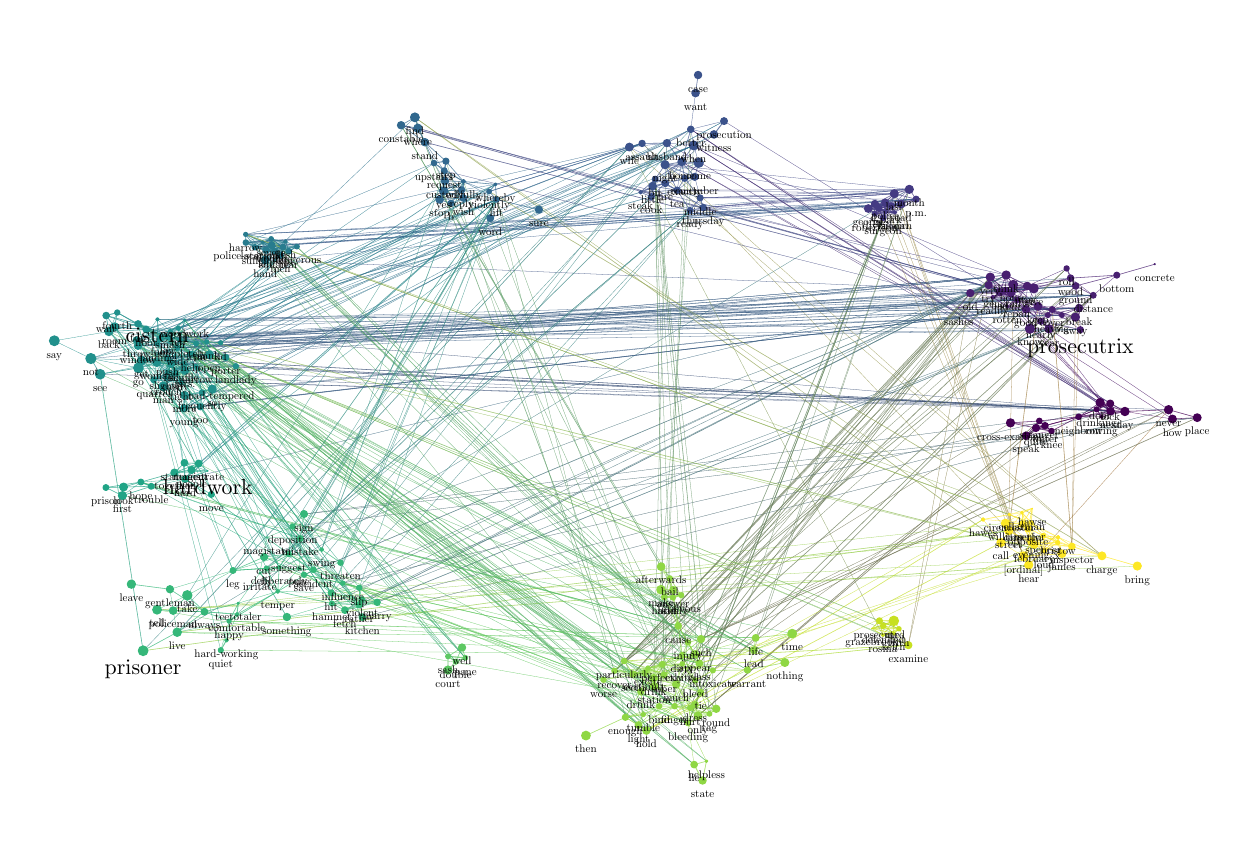
\begin{tikzpicture}[x=1pt,y=1pt]
\definecolor{fillColor}{RGB}{255,255,255}
\path[use as bounding box,fill=fillColor,fill opacity=0.00] (0,0) rectangle (433.62,289.08);
\begin{scope}
\path[clip] (  0.00,  0.00) rectangle (433.62,289.08);
\definecolor{drawColor}{RGB}{33,144,140}

\path[draw=drawColor,draw opacity=0.50,line width= 0.1pt,line join=round,line cap=round] (  9.64,175.94) -- ( 22.83,169.52);

\path[draw=drawColor,draw opacity=0.50,line width= 0.1pt,line join=round,line cap=round] ( 40.02,166.14) -- ( 22.83,169.52);

\path[draw=drawColor,draw opacity=0.50,line width= 0.2pt,line join=round,line cap=round] ( 26.19,163.85) -- ( 22.83,169.52);
\definecolor{drawColor}{RGB}{46,113,139}

\path[draw=drawColor,draw opacity=0.50,line width= 0.1pt,line join=round,line cap=round] (240.66,246.53) -- ( 22.83,169.52);
\definecolor{drawColor}{RGB}{33,144,140}

\path[draw=drawColor,draw opacity=0.50,line width= 0.1pt,line join=round,line cap=round] ( 41.15,168.75) -- ( 22.83,169.52);
\definecolor{drawColor}{RGB}{52,87,126}

\path[draw=drawColor,draw opacity=0.50,line width= 0.1pt,line join=round,line cap=round] (353.57,199.69) -- ( 22.83,169.52);
\definecolor{drawColor}{RGB}{33,144,140}

\path[draw=drawColor,draw opacity=0.50,line width= 0.1pt,line join=round,line cap=round] ( 39.86,174.13) -- ( 22.83,169.52);
\definecolor{drawColor}{RGB}{88,179,104}

\path[draw=drawColor,draw opacity=0.50,line width= 0.1pt,line join=round,line cap=round] (226.22, 54.02) -- ( 22.83,169.52);
\definecolor{drawColor}{RGB}{33,144,140}

\path[draw=drawColor,draw opacity=0.50,line width= 0.1pt,line join=round,line cap=round] ( 22.83,169.52) -- (  9.64,175.94);

\path[draw=drawColor,draw opacity=0.50,line width= 0.1pt,line join=round,line cap=round] ( 29.35,179.29) -- (  9.64,175.94);
\definecolor{drawColor}{RGB}{43,163,130}

\path[draw=drawColor,draw opacity=0.50,line width= 0.2pt,line join=round,line cap=round] ( 26.19,163.85) -- ( 41.71, 63.93);
\definecolor{drawColor}{RGB}{53,183,121}

\path[draw=drawColor,draw opacity=0.50,line width= 0.2pt,line join=round,line cap=round] ( 54.03, 70.63) -- ( 41.71, 63.93);
\definecolor{drawColor}{RGB}{153,207,79}

\path[draw=drawColor,draw opacity=0.50,line width= 0.2pt,line join=round,line cap=round] (354.49,107.30) -- ( 41.71, 63.93);
\definecolor{drawColor}{RGB}{56,132,130}

\path[draw=drawColor,draw opacity=0.50,line width= 0.1pt,line join=round,line cap=round] (217.43,245.94) -- ( 41.71, 63.93);
\definecolor{drawColor}{RGB}{33,144,140}

\path[draw=drawColor,draw opacity=0.50,line width= 0.1pt,line join=round,line cap=round] ( 22.83,169.52) -- ( 40.02,166.14);

\path[draw=drawColor,draw opacity=0.50,line width= 0.2pt,line join=round,line cap=round] ( 26.19,163.85) -- ( 40.02,166.14);

\path[draw=drawColor,draw opacity=0.50,line width= 0.1pt,line join=round,line cap=round] ( 41.15,168.75) -- ( 40.02,166.14);

\path[draw=drawColor,draw opacity=0.50,line width= 0.1pt,line join=round,line cap=round] ( 56.83,165.19) -- ( 40.02,166.14);

\path[draw=drawColor,draw opacity=0.50,line width= 0.1pt,line join=round,line cap=round] ( 65.64,170.92) -- ( 40.02,166.14);

\path[draw=drawColor,draw opacity=0.50,line width= 0.1pt,line join=round,line cap=round] ( 46.61,168.02) -- ( 40.02,166.14);

\path[draw=drawColor,draw opacity=0.50,line width= 0.1pt,line join=round,line cap=round] ( 58.96,171.11) -- ( 40.02,166.14);

\path[draw=drawColor,draw opacity=0.50,line width= 0.2pt,line join=round,line cap=round] ( 22.83,169.52) -- ( 26.19,163.85);
\definecolor{drawColor}{RGB}{43,163,130}

\path[draw=drawColor,draw opacity=0.50,line width= 0.2pt,line join=round,line cap=round] ( 41.71, 63.93) -- ( 26.19,163.85);
\definecolor{drawColor}{RGB}{33,144,140}

\path[draw=drawColor,draw opacity=0.50,line width= 0.2pt,line join=round,line cap=round] ( 40.02,166.14) -- ( 26.19,163.85);
\definecolor{drawColor}{RGB}{50,72,112}

\path[draw=drawColor,draw opacity=0.50,line width= 0.1pt,line join=round,line cap=round] (412.27,151.03) -- ( 26.19,163.85);
\definecolor{drawColor}{RGB}{33,144,140}

\path[draw=drawColor,draw opacity=0.50,line width= 0.1pt,line join=round,line cap=round] ( 46.61,168.02) -- ( 26.19,163.85);
\definecolor{drawColor}{RGB}{88,179,104}

\path[draw=drawColor,draw opacity=0.50,line width= 0.1pt,line join=round,line cap=round] (262.39, 64.12) -- ( 26.19,163.85);
\definecolor{drawColor}{RGB}{199,224,32}

\path[draw=drawColor,draw opacity=0.50,line width= 0.3pt,line join=round,line cap=round] (307.79, 74.75) -- (312.98, 74.73);

\path[draw=drawColor,draw opacity=0.50,line width= 0.3pt,line join=round,line cap=round] (309.13, 72.93) -- (312.98, 74.73);

\path[draw=drawColor,draw opacity=0.50,line width= 0.2pt,line join=round,line cap=round] (314.86, 71.85) -- (312.98, 74.73);

\path[draw=drawColor,draw opacity=0.50,line width= 0.2pt,line join=round,line cap=round] (312.92, 70.24) -- (312.98, 74.73);

\path[draw=drawColor,draw opacity=0.50,line width= 0.2pt,line join=round,line cap=round] (309.02, 69.58) -- (312.98, 74.73);

\path[draw=drawColor,draw opacity=0.50,line width= 0.2pt,line join=round,line cap=round] (305.08, 71.98) -- (312.98, 74.73);
\definecolor{drawColor}{RGB}{53,183,121}

\path[draw=drawColor,draw opacity=0.50,line width= 0.1pt,line join=round,line cap=round] ( 46.75, 78.75) -- ( 57.69, 83.96);

\path[draw=drawColor,draw opacity=0.50,line width= 0.2pt,line join=round,line cap=round] ( 52.56, 78.43) -- ( 57.69, 83.96);
\definecolor{drawColor}{RGB}{51,143,131}

\path[draw=drawColor,draw opacity=0.50,line width= 0.1pt,line join=round,line cap=round] (150.77,233.69) -- ( 57.69, 83.96);
\definecolor{drawColor}{RGB}{53,183,121}

\path[draw=drawColor,draw opacity=0.50,line width= 0.2pt,line join=round,line cap=round] ( 63.87, 78.03) -- ( 57.69, 83.96);

\path[draw=drawColor,draw opacity=0.50,line width= 0.1pt,line join=round,line cap=round] ( 74.19, 92.93) -- ( 57.69, 83.96);
\definecolor{drawColor}{RGB}{59,82,139}

\path[draw=drawColor,draw opacity=0.50,line width= 0.1pt,line join=round,line cap=round] (240.66,246.53) -- (242.48,240.28);
\definecolor{drawColor}{RGB}{46,113,139}

\path[draw=drawColor,draw opacity=0.50,line width= 0.1pt,line join=round,line cap=round] ( 41.15,168.75) -- (242.48,240.28);
\definecolor{drawColor}{RGB}{59,82,139}

\path[draw=drawColor,draw opacity=0.50,line width= 0.2pt,line join=round,line cap=round] (230.32,239.56) -- (242.48,240.28);

\path[draw=drawColor,draw opacity=0.50,line width= 0.2pt,line join=round,line cap=round] (236.32,240.58) -- (242.48,240.28);

\path[draw=drawColor,draw opacity=0.50,line width= 0.2pt,line join=round,line cap=round] (241.04,235.17) -- (242.48,240.28);

\path[draw=drawColor,draw opacity=0.50,line width= 0.1pt,line join=round,line cap=round] (237.42,234.65) -- (242.48,240.28);
\definecolor{drawColor}{RGB}{253,231,37}

\path[draw=drawColor,draw opacity=0.50,line width= 0.1pt,line join=round,line cap=round] (351.70,103.01) -- (359.85, 98.04);

\path[draw=drawColor,draw opacity=0.50,line width= 0.1pt,line join=round,line cap=round] (361.73, 94.94) -- (359.85, 98.04);
\definecolor{drawColor}{RGB}{160,144,84}

\path[draw=drawColor,draw opacity=0.50,line width= 0.1pt,line join=round,line cap=round] (313.15,229.10) -- (359.85, 98.04);
\definecolor{drawColor}{RGB}{253,231,37}

\path[draw=drawColor,draw opacity=0.50,line width= 0.2pt,line join=round,line cap=round] (373.73, 99.00) -- (359.85, 98.04);
\definecolor{drawColor}{RGB}{160,144,84}

\path[draw=drawColor,draw opacity=0.50,line width= 0.1pt,line join=round,line cap=round] (315.61,225.39) -- (359.85, 98.04);
\definecolor{drawColor}{RGB}{253,231,37}

\path[draw=drawColor,draw opacity=0.50,line width= 0.3pt,line join=round,line cap=round] (362.62,103.34) -- (359.85, 98.04);
\definecolor{drawColor}{RGB}{160,144,84}

\path[draw=drawColor,draw opacity=0.50,line width= 0.1pt,line join=round,line cap=round] (309.87,225.84) -- (359.85, 98.04);

\path[draw=drawColor,draw opacity=0.50,line width= 0.1pt,line join=round,line cap=round] (306.15,225.39) -- (359.85, 98.04);
\definecolor{drawColor}{RGB}{253,231,37}

\path[draw=drawColor,draw opacity=0.50,line width= 0.2pt,line join=round,line cap=round] (363.72,102.19) -- (359.85, 98.04);
\definecolor{drawColor}{RGB}{160,144,84}

\path[draw=drawColor,draw opacity=0.50,line width= 0.1pt,line join=round,line cap=round] (312.02,224.70) -- (359.85, 98.04);
\definecolor{drawColor}{RGB}{72,31,112}

\path[draw=drawColor,draw opacity=0.50,line width= 0.2pt,line join=round,line cap=round] (369.05,180.25) -- (362.16,180.29);
\definecolor{drawColor}{RGB}{70,16,97}

\path[draw=drawColor,draw opacity=0.50,line width= 0.1pt,line join=round,line cap=round] (413.66,147.68) -- (362.16,180.29);
\definecolor{drawColor}{RGB}{72,31,112}

\path[draw=drawColor,draw opacity=0.50,line width= 0.2pt,line join=round,line cap=round] (365.08,188.38) -- (362.16,180.29);

\path[draw=drawColor,draw opacity=0.50,line width= 0.1pt,line join=round,line cap=round] (360.72,187.31) -- (362.16,180.29);

\path[draw=drawColor,draw opacity=0.50,line width= 0.2pt,line join=round,line cap=round] (366.09,182.97) -- (362.16,180.29);

\path[draw=drawColor,draw opacity=0.50,line width= 0.1pt,line join=round,line cap=round] (370.22,187.23) -- (362.16,180.29);

\path[draw=drawColor,draw opacity=0.50,line width= 0.1pt,line join=round,line cap=round] (356.14,196.19) -- (363.55,194.89);

\path[draw=drawColor,draw opacity=0.50,line width= 0.1pt,line join=round,line cap=round] (353.57,199.69) -- (363.55,194.89);

\path[draw=drawColor,draw opacity=0.50,line width= 0.1pt,line join=round,line cap=round] (365.08,188.38) -- (363.55,194.89);

\path[draw=drawColor,draw opacity=0.50,line width= 0.1pt,line join=round,line cap=round] (360.72,187.31) -- (363.55,194.89);

\path[draw=drawColor,draw opacity=0.50,line width= 0.3pt,line join=round,line cap=round] (361.18,195.74) -- (363.55,194.89);

\path[draw=drawColor,draw opacity=0.50,line width= 0.2pt,line join=round,line cap=round] (351.28,193.54) -- (363.55,194.89);

\path[draw=drawColor,draw opacity=0.50,line width= 0.2pt,line join=round,line cap=round] (355.31,193.07) -- (363.55,194.89);

\path[draw=drawColor,draw opacity=0.50,line width= 0.1pt,line join=round,line cap=round] (378.70,195.75) -- (363.55,194.89);

\path[draw=drawColor,draw opacity=0.50,line width= 0.2pt,line join=round,line cap=round] (376.84,198.57) -- (363.55,194.89);

\path[draw=drawColor,draw opacity=0.50,line width= 0.2pt,line join=round,line cap=round] (353.31,194.23) -- (363.55,194.89);

\path[draw=drawColor,draw opacity=0.50,line width= 0.1pt,line join=round,line cap=round] (348.73,191.71) -- (363.55,194.89);
\definecolor{drawColor}{RGB}{46,113,139}

\path[draw=drawColor,draw opacity=0.50,line width= 0.1pt,line join=round,line cap=round] ( 22.83,169.52) -- (240.66,246.53);
\definecolor{drawColor}{RGB}{59,82,139}

\path[draw=drawColor,draw opacity=0.50,line width= 0.1pt,line join=round,line cap=round] (242.48,240.28) -- (240.66,246.53);
\definecolor{drawColor}{RGB}{46,113,139}

\path[draw=drawColor,draw opacity=0.50,line width= 0.2pt,line join=round,line cap=round] ( 41.15,168.75) -- (240.66,246.53);
\definecolor{drawColor}{RGB}{63,41,111}

\path[draw=drawColor,draw opacity=0.50,line width= 0.1pt,line join=round,line cap=round] (387.52,153.60) -- (240.66,246.53);
\definecolor{drawColor}{RGB}{65,56,125}

\path[draw=drawColor,draw opacity=0.50,line width= 0.1pt,line join=round,line cap=round] (353.57,199.69) -- (240.66,246.53);
\definecolor{drawColor}{RGB}{46,113,139}

\path[draw=drawColor,draw opacity=0.50,line width= 0.1pt,line join=round,line cap=round] ( 56.83,165.19) -- (240.66,246.53);
\definecolor{drawColor}{RGB}{59,82,139}

\path[draw=drawColor,draw opacity=0.50,line width= 0.2pt,line join=round,line cap=round] (236.32,240.58) -- (240.66,246.53);
\definecolor{drawColor}{RGB}{63,41,111}

\path[draw=drawColor,draw opacity=0.50,line width= 0.2pt,line join=round,line cap=round] (391.30,150.50) -- (240.66,246.53);
\definecolor{drawColor}{RGB}{59,82,139}

\path[draw=drawColor,draw opacity=0.50,line width= 0.1pt,line join=round,line cap=round] (230.99,247.37) -- (240.66,246.53);
\definecolor{drawColor}{RGB}{101,148,103}

\path[draw=drawColor,draw opacity=0.50,line width= 0.1pt,line join=round,line cap=round] (226.22, 54.02) -- (240.66,246.53);
\definecolor{drawColor}{RGB}{59,82,139}

\path[draw=drawColor,draw opacity=0.50,line width= 0.1pt,line join=round,line cap=round] (239.61,252.35) -- (240.66,246.53);
\definecolor{drawColor}{RGB}{46,113,139}

\path[draw=drawColor,draw opacity=0.50,line width= 0.1pt,line join=round,line cap=round] ( 50.55,169.58) -- (240.66,246.53);

\path[draw=drawColor,draw opacity=0.50,line width= 0.1pt,line join=round,line cap=round] ( 45.53,161.84) -- (240.66,246.53);
\definecolor{drawColor}{RGB}{33,144,140}

\path[draw=drawColor,draw opacity=0.50,line width= 0.1pt,line join=round,line cap=round] ( 41.15,168.75) -- ( 49.04,159.47);

\path[draw=drawColor,draw opacity=0.50,line width= 0.2pt,line join=round,line cap=round] ( 56.83,165.19) -- ( 49.04,159.47);

\path[draw=drawColor,draw opacity=0.50,line width= 0.1pt,line join=round,line cap=round] ( 56.72,156.20) -- ( 49.04,159.47);

\path[draw=drawColor,draw opacity=0.50,line width= 0.1pt,line join=round,line cap=round] ( 46.61,168.02) -- ( 49.04,159.47);

\path[draw=drawColor,draw opacity=0.50,line width= 0.1pt,line join=round,line cap=round] ( 56.53,151.56) -- ( 49.04,159.47);

\path[draw=drawColor,draw opacity=0.50,line width= 0.1pt,line join=round,line cap=round] ( 51.88,167.56) -- ( 49.04,159.47);

\path[draw=drawColor,draw opacity=0.50,line width= 0.2pt,line join=round,line cap=round] ( 53.41,164.05) -- ( 49.04,159.47);

\path[draw=drawColor,draw opacity=0.50,line width= 0.1pt,line join=round,line cap=round] ( 50.37,164.47) -- ( 49.04,159.47);

\path[draw=drawColor,draw opacity=0.50,line width= 0.1pt,line join=round,line cap=round] ( 55.51,160.74) -- ( 49.04,159.47);

\path[draw=drawColor,draw opacity=0.50,line width= 0.1pt,line join=round,line cap=round] ( 22.83,169.52) -- ( 41.15,168.75);

\path[draw=drawColor,draw opacity=0.50,line width= 0.1pt,line join=round,line cap=round] ( 40.02,166.14) -- ( 41.15,168.75);
\definecolor{drawColor}{RGB}{46,113,139}

\path[draw=drawColor,draw opacity=0.50,line width= 0.1pt,line join=round,line cap=round] (242.48,240.28) -- ( 41.15,168.75);

\path[draw=drawColor,draw opacity=0.50,line width= 0.2pt,line join=round,line cap=round] (240.66,246.53) -- ( 41.15,168.75);
\definecolor{drawColor}{RGB}{33,144,140}

\path[draw=drawColor,draw opacity=0.50,line width= 0.1pt,line join=round,line cap=round] ( 49.04,159.47) -- ( 41.15,168.75);
\definecolor{drawColor}{RGB}{52,87,126}

\path[draw=drawColor,draw opacity=0.50,line width= 0.1pt,line join=round,line cap=round] (347.83,198.93) -- ( 41.15,168.75);
\definecolor{drawColor}{RGB}{33,144,140}

\path[draw=drawColor,draw opacity=0.50,line width= 0.1pt,line join=round,line cap=round] ( 29.35,179.29) -- ( 41.15,168.75);

\path[draw=drawColor,draw opacity=0.50,line width= 0.2pt,line join=round,line cap=round] ( 31.41,180.98) -- ( 41.15,168.75);

\path[draw=drawColor,draw opacity=0.50,line width= 0.2pt,line join=round,line cap=round] ( 56.83,165.19) -- ( 41.15,168.75);

\path[draw=drawColor,draw opacity=0.50,line width= 0.1pt,line join=round,line cap=round] ( 56.72,156.20) -- ( 41.15,168.75);

\path[draw=drawColor,draw opacity=0.50,line width= 0.1pt,line join=round,line cap=round] ( 46.61,168.02) -- ( 41.15,168.75);
\definecolor{drawColor}{RGB}{50,72,112}

\path[draw=drawColor,draw opacity=0.50,line width= 0.2pt,line join=round,line cap=round] (391.30,150.50) -- ( 41.15,168.75);
\definecolor{drawColor}{RGB}{33,144,140}

\path[draw=drawColor,draw opacity=0.50,line width= 0.2pt,line join=round,line cap=round] ( 51.88,167.56) -- ( 41.15,168.75);

\path[draw=drawColor,draw opacity=0.50,line width= 0.2pt,line join=round,line cap=round] ( 58.96,171.11) -- ( 41.15,168.75);

\path[draw=drawColor,draw opacity=0.50,line width= 0.1pt,line join=round,line cap=round] ( 50.55,169.58) -- ( 41.15,168.75);
\definecolor{drawColor}{RGB}{49,104,142}

\path[draw=drawColor,draw opacity=0.50,line width= 0.2pt,line join=round,line cap=round] (140.99,252.74) -- (139.92,256.67);
\definecolor{drawColor}{RGB}{151,167,89}

\path[draw=drawColor,draw opacity=0.50,line width= 0.2pt,line join=round,line cap=round] (351.70,103.01) -- (139.92,256.67);
\definecolor{drawColor}{RGB}{44,113,142}

\path[draw=drawColor,draw opacity=0.50,line width= 0.1pt,line join=round,line cap=round] ( 85.86,205.12) -- (139.92,256.67);
\definecolor{drawColor}{RGB}{96,159,105}

\path[draw=drawColor,draw opacity=0.50,line width= 0.2pt,line join=round,line cap=round] (223.58, 35.09) -- (139.92,256.67);
\definecolor{drawColor}{RGB}{49,104,142}

\path[draw=drawColor,draw opacity=0.50,line width= 0.1pt,line join=round,line cap=round] (143.52,247.69) -- (139.92,256.67);

\path[draw=drawColor,draw opacity=0.50,line width= 0.2pt,line join=round,line cap=round] (134.93,253.82) -- (139.92,256.67);
\definecolor{drawColor}{RGB}{151,167,89}

\path[draw=drawColor,draw opacity=0.50,line width= 0.1pt,line join=round,line cap=round] (345.23,111.35) -- (139.92,256.67);
\definecolor{drawColor}{RGB}{72,31,112}

\path[draw=drawColor,draw opacity=0.50,line width= 0.1pt,line join=round,line cap=round] (363.55,194.89) -- (356.14,196.19);

\path[draw=drawColor,draw opacity=0.50,line width= 0.1pt,line join=round,line cap=round] (353.57,199.69) -- (356.14,196.19);
\definecolor{drawColor}{RGB}{162,131,74}

\path[draw=drawColor,draw opacity=0.50,line width= 0.1pt,line join=round,line cap=round] (354.49,107.30) -- (356.14,196.19);
\definecolor{drawColor}{RGB}{72,31,112}

\path[draw=drawColor,draw opacity=0.50,line width= 0.2pt,line join=round,line cap=round] (365.08,188.38) -- (356.14,196.19);

\path[draw=drawColor,draw opacity=0.50,line width= 0.1pt,line join=round,line cap=round] (361.18,195.74) -- (356.14,196.19);

\path[draw=drawColor,draw opacity=0.50,line width= 0.2pt,line join=round,line cap=round] (351.28,193.54) -- (356.14,196.19);
\definecolor{drawColor}{RGB}{60,67,127}

\path[draw=drawColor,draw opacity=0.50,line width= 0.1pt,line join=round,line cap=round] (134.93,253.82) -- (356.14,196.19);
\definecolor{drawColor}{RGB}{72,31,112}

\path[draw=drawColor,draw opacity=0.50,line width= 0.1pt,line join=round,line cap=round] (347.24,196.07) -- (356.14,196.19);

\path[draw=drawColor,draw opacity=0.50,line width= 0.2pt,line join=round,line cap=round] (355.31,193.07) -- (356.14,196.19);

\path[draw=drawColor,draw opacity=0.50,line width= 0.2pt,line join=round,line cap=round] (353.31,194.23) -- (356.14,196.19);

\path[draw=drawColor,draw opacity=0.50,line width= 0.1pt,line join=round,line cap=round] (357.56,190.66) -- (356.14,196.19);

\path[draw=drawColor,draw opacity=0.50,line width= 0.1pt,line join=round,line cap=round] (348.73,191.71) -- (356.14,196.19);
\definecolor{drawColor}{RGB}{53,183,121}

\path[draw=drawColor,draw opacity=0.50,line width= 0.1pt,line join=round,line cap=round] ( 57.69, 83.96) -- ( 46.75, 78.75);
\definecolor{drawColor}{RGB}{153,207,79}

\path[draw=drawColor,draw opacity=0.50,line width= 0.1pt,line join=round,line cap=round] (400.96, 94.54) -- ( 46.75, 78.75);

\path[draw=drawColor,draw opacity=0.50,line width= 0.1pt,line join=round,line cap=round] (388.19, 98.22) -- ( 46.75, 78.75);
\definecolor{drawColor}{RGB}{53,183,121}

\path[draw=drawColor,draw opacity=0.50,line width= 0.1pt,line join=round,line cap=round] ( 52.56, 78.43) -- ( 46.75, 78.75);

\path[draw=drawColor,draw opacity=0.50,line width= 0.1pt,line join=round,line cap=round] ( 63.87, 78.03) -- ( 46.75, 78.75);
\definecolor{drawColor}{RGB}{98,199,94}

\path[draw=drawColor,draw opacity=0.50,line width= 0.1pt,line join=round,line cap=round] (241.12, 44.46) -- ( 46.75, 78.75);
\definecolor{drawColor}{RGB}{143,215,68}

\path[draw=drawColor,draw opacity=0.50,line width= 0.2pt,line join=round,line cap=round] (215.98, 39.89) -- (201.73, 33.28);
\definecolor{drawColor}{RGB}{87,189,101}

\path[draw=drawColor,draw opacity=0.50,line width= 0.1pt,line join=round,line cap=round] ( 34.24,119.99) -- (276.25, 70.12);
\definecolor{drawColor}{RGB}{143,215,68}

\path[draw=drawColor,draw opacity=0.50,line width= 0.2pt,line join=round,line cap=round] (262.39, 64.12) -- (276.25, 70.12);

\path[draw=drawColor,draw opacity=0.50,line width= 0.2pt,line join=round,line cap=round] (263.07, 68.58) -- (276.25, 70.12);

\path[draw=drawColor,draw opacity=0.50,line width= 0.1pt,line join=round,line cap=round] (228.89, 94.32) -- (228.83, 86.00);

\path[draw=drawColor,draw opacity=0.50,line width= 0.3pt,line join=round,line cap=round] (233.20, 85.90) -- (228.83, 86.00);

\path[draw=drawColor,draw opacity=0.50,line width= 0.1pt,line join=round,line cap=round] (235.08, 72.90) -- (228.83, 86.00);

\path[draw=drawColor,draw opacity=0.50,line width= 0.2pt,line join=round,line cap=round] (230.01, 83.36) -- (228.83, 86.00);

\path[draw=drawColor,draw opacity=0.50,line width= 0.2pt,line join=round,line cap=round] (233.17, 83.16) -- (228.83, 86.00);

\path[draw=drawColor,draw opacity=0.50,line width= 0.2pt,line join=round,line cap=round] (236.18, 84.01) -- (228.83, 86.00);
\definecolor{drawColor}{RGB}{53,183,121}

\path[draw=drawColor,draw opacity=0.50,line width= 0.2pt,line join=round,line cap=round] ( 41.71, 63.93) -- ( 54.03, 70.63);
\definecolor{drawColor}{RGB}{153,207,79}

\path[draw=drawColor,draw opacity=0.50,line width= 0.2pt,line join=round,line cap=round] (354.49,107.30) -- ( 54.03, 70.63);
\definecolor{drawColor}{RGB}{60,120,125}

\path[draw=drawColor,draw opacity=0.50,line width= 0.1pt,line join=round,line cap=round] (318.58,230.66) -- ( 54.03, 70.63);
\definecolor{drawColor}{RGB}{56,132,130}

\path[draw=drawColor,draw opacity=0.50,line width= 0.2pt,line join=round,line cap=round] (217.43,245.94) -- ( 54.03, 70.63);
\definecolor{drawColor}{RGB}{53,183,121}

\path[draw=drawColor,draw opacity=0.50,line width= 0.1pt,line join=round,line cap=round] ( 52.56, 78.43) -- ( 54.03, 70.63);
\definecolor{drawColor}{RGB}{98,199,94}

\path[draw=drawColor,draw opacity=0.50,line width= 0.1pt,line join=round,line cap=round] (241.14, 62.67) -- ( 54.03, 70.63);
\definecolor{drawColor}{RGB}{53,183,121}

\path[draw=drawColor,draw opacity=0.50,line width= 0.2pt,line join=round,line cap=round] ( 63.87, 78.03) -- ( 54.03, 70.63);
\definecolor{drawColor}{RGB}{98,199,94}

\path[draw=drawColor,draw opacity=0.50,line width= 0.1pt,line join=round,line cap=round] (263.07, 68.58) -- ( 54.03, 70.63);
\definecolor{drawColor}{RGB}{53,183,121}

\path[draw=drawColor,draw opacity=0.50,line width= 0.1pt,line join=round,line cap=round] ( 72.80, 74.63) -- ( 54.03, 70.63);
\definecolor{drawColor}{RGB}{68,1,84}

\path[draw=drawColor,draw opacity=0.50,line width= 0.2pt,line join=round,line cap=round] (412.27,151.03) -- (396.49,150.39);

\path[draw=drawColor,draw opacity=0.50,line width= 0.2pt,line join=round,line cap=round] (387.52,153.60) -- (396.49,150.39);

\path[draw=drawColor,draw opacity=0.50,line width= 0.1pt,line join=round,line cap=round] (413.66,147.68) -- (396.49,150.39);

\path[draw=drawColor,draw opacity=0.50,line width= 0.2pt,line join=round,line cap=round] (391.30,150.50) -- (396.49,150.39);
\definecolor{drawColor}{RGB}{63,41,111}

\path[draw=drawColor,draw opacity=0.50,line width= 0.1pt,line join=round,line cap=round] (230.99,247.37) -- (396.49,150.39);
\definecolor{drawColor}{RGB}{68,1,84}

\path[draw=drawColor,draw opacity=0.50,line width= 0.2pt,line join=round,line cap=round] (391.18,153.26) -- (396.49,150.39);

\path[draw=drawColor,draw opacity=0.50,line width= 0.2pt,line join=round,line cap=round] (379.76,148.48) -- (396.49,150.39);

\path[draw=drawColor,draw opacity=0.50,line width= 0.2pt,line join=round,line cap=round] (386.24,151.15) -- (396.49,150.39);

\path[draw=drawColor,draw opacity=0.50,line width= 0.2pt,line join=round,line cap=round] (388.05,148.47) -- (396.49,150.39);
\definecolor{drawColor}{RGB}{50,72,112}

\path[draw=drawColor,draw opacity=0.50,line width= 0.1pt,line join=round,line cap=round] ( 26.19,163.85) -- (412.27,151.03);
\definecolor{drawColor}{RGB}{68,1,84}

\path[draw=drawColor,draw opacity=0.50,line width= 0.2pt,line join=round,line cap=round] (396.49,150.39) -- (412.27,151.03);
\definecolor{drawColor}{RGB}{70,16,97}

\path[draw=drawColor,draw opacity=0.50,line width= 0.1pt,line join=round,line cap=round] (369.05,180.25) -- (412.27,151.03);
\definecolor{drawColor}{RGB}{160,116,60}

\path[draw=drawColor,draw opacity=0.50,line width= 0.1pt,line join=round,line cap=round] (361.73, 94.94) -- (412.27,151.03);
\definecolor{drawColor}{RGB}{68,1,84}

\path[draw=drawColor,draw opacity=0.50,line width= 0.1pt,line join=round,line cap=round] (413.66,147.68) -- (412.27,151.03);

\path[draw=drawColor,draw opacity=0.50,line width= 0.2pt,line join=round,line cap=round] (422.61,148.16) -- (412.27,151.03);
\definecolor{drawColor}{RGB}{105,108,76}

\path[draw=drawColor,draw opacity=0.50,line width= 0.1pt,line join=round,line cap=round] (226.22, 54.02) -- (412.27,151.03);

\path[draw=drawColor,draw opacity=0.50,line width= 0.1pt,line join=round,line cap=round] (243.33, 68.16) -- (412.27,151.03);
\definecolor{drawColor}{RGB}{60,92,102}

\path[draw=drawColor,draw opacity=0.50,line width= 0.1pt,line join=round,line cap=round] (120.93, 76.07) -- (412.27,151.03);
\definecolor{drawColor}{RGB}{63,41,111}

\path[draw=drawColor,draw opacity=0.50,line width= 0.1pt,line join=round,line cap=round] (240.66,246.53) -- (387.52,153.60);
\definecolor{drawColor}{RGB}{68,1,84}

\path[draw=drawColor,draw opacity=0.50,line width= 0.2pt,line join=round,line cap=round] (396.49,150.39) -- (387.52,153.60);
\definecolor{drawColor}{RGB}{63,41,111}

\path[draw=drawColor,draw opacity=0.50,line width= 0.1pt,line join=round,line cap=round] (236.32,240.58) -- (387.52,153.60);
\definecolor{drawColor}{RGB}{68,1,84}

\path[draw=drawColor,draw opacity=0.50,line width= 0.2pt,line join=round,line cap=round] (391.30,150.50) -- (387.52,153.60);

\path[draw=drawColor,draw opacity=0.50,line width= 0.2pt,line join=round,line cap=round] (391.18,153.26) -- (387.52,153.60);
\definecolor{drawColor}{RGB}{63,41,111}

\path[draw=drawColor,draw opacity=0.50,line width= 0.1pt,line join=round,line cap=round] (239.61,252.35) -- (387.52,153.60);
\definecolor{drawColor}{RGB}{68,1,84}

\path[draw=drawColor,draw opacity=0.50,line width= 0.2pt,line join=round,line cap=round] (379.76,148.48) -- (387.52,153.60);

\path[draw=drawColor,draw opacity=0.50,line width= 0.2pt,line join=round,line cap=round] (386.24,151.15) -- (387.52,153.60);

\path[draw=drawColor,draw opacity=0.50,line width= 0.2pt,line join=round,line cap=round] (388.05,148.47) -- (387.52,153.60);
\definecolor{drawColor}{RGB}{253,231,37}

\path[draw=drawColor,draw opacity=0.50,line width= 0.2pt,line join=round,line cap=round] (354.49,107.30) -- (353.32,109.98);
\definecolor{drawColor}{RGB}{153,207,79}

\path[draw=drawColor,draw opacity=0.50,line width= 0.1pt,line join=round,line cap=round] ( 52.56, 78.43) -- (353.32,109.98);
\definecolor{drawColor}{RGB}{253,231,37}

\path[draw=drawColor,draw opacity=0.50,line width= 0.1pt,line join=round,line cap=round] (362.62,103.34) -- (353.32,109.98);

\path[draw=drawColor,draw opacity=0.50,line width= 0.2pt,line join=round,line cap=round] (361.49,108.05) -- (353.32,109.98);

\path[draw=drawColor,draw opacity=0.50,line width= 0.2pt,line join=round,line cap=round] (359.29,109.73) -- (353.32,109.98);

\path[draw=drawColor,draw opacity=0.50,line width= 0.2pt,line join=round,line cap=round] (362.68,110.13) -- (353.32,109.98);

\path[draw=drawColor,draw opacity=0.50,line width= 0.1pt,line join=round,line cap=round] (359.29,113.78) -- (353.32,109.98);
\definecolor{drawColor}{RGB}{53,183,121}

\path[draw=drawColor,draw opacity=0.50,line width= 0.2pt,line join=round,line cap=round] ( 51.41, 86.16) -- ( 37.47, 87.99);
\definecolor{drawColor}{RGB}{52,87,126}

\path[draw=drawColor,draw opacity=0.50,line width= 0.1pt,line join=round,line cap=round] ( 41.15,168.75) -- (347.83,198.93);
\definecolor{drawColor}{RGB}{72,31,112}

\path[draw=drawColor,draw opacity=0.50,line width= 0.1pt,line join=round,line cap=round] (353.57,199.69) -- (347.83,198.93);
\definecolor{drawColor}{RGB}{52,87,126}

\path[draw=drawColor,draw opacity=0.50,line width= 0.1pt,line join=round,line cap=round] ( 46.61,168.02) -- (347.83,198.93);
\definecolor{drawColor}{RGB}{70,16,97}

\path[draw=drawColor,draw opacity=0.50,line width= 0.1pt,line join=round,line cap=round] (391.30,150.50) -- (347.83,198.93);
\definecolor{drawColor}{RGB}{72,31,112}

\path[draw=drawColor,draw opacity=0.50,line width= 0.1pt,line join=round,line cap=round] (361.18,195.74) -- (347.83,198.93);
\definecolor{drawColor}{RGB}{52,87,126}

\path[draw=drawColor,draw opacity=0.50,line width= 0.1pt,line join=round,line cap=round] ( 39.86,174.13) -- (347.83,198.93);
\definecolor{drawColor}{RGB}{72,31,112}

\path[draw=drawColor,draw opacity=0.50,line width= 0.2pt,line join=round,line cap=round] (351.28,193.54) -- (347.83,198.93);
\definecolor{drawColor}{RGB}{107,123,89}

\path[draw=drawColor,draw opacity=0.50,line width= 0.2pt,line join=round,line cap=round] (234.34, 51.74) -- (347.83,198.93);
\definecolor{drawColor}{RGB}{72,31,112}

\path[draw=drawColor,draw opacity=0.50,line width= 0.1pt,line join=round,line cap=round] (347.24,196.07) -- (347.83,198.93);
\definecolor{drawColor}{RGB}{107,123,89}

\path[draw=drawColor,draw opacity=0.50,line width= 0.1pt,line join=round,line cap=round] (226.22, 54.02) -- (347.83,198.93);
\definecolor{drawColor}{RGB}{135,127,72}

\path[draw=drawColor,draw opacity=0.50,line width= 0.1pt,line join=round,line cap=round] (318.23, 65.95) -- (347.83,198.93);
\definecolor{drawColor}{RGB}{107,123,89}

\path[draw=drawColor,draw opacity=0.50,line width= 0.1pt,line join=round,line cap=round] (242.73, 59.38) -- (347.83,198.93);

\path[draw=drawColor,draw opacity=0.50,line width= 0.2pt,line join=round,line cap=round] (218.76, 55.51) -- (347.83,198.93);
\definecolor{drawColor}{RGB}{52,87,126}

\path[draw=drawColor,draw opacity=0.50,line width= 0.1pt,line join=round,line cap=round] ( 50.55,169.58) -- (347.83,198.93);
\definecolor{drawColor}{RGB}{72,31,112}

\path[draw=drawColor,draw opacity=0.50,line width= 0.1pt,line join=round,line cap=round] (353.31,194.23) -- (347.83,198.93);
\definecolor{drawColor}{RGB}{107,123,89}

\path[draw=drawColor,draw opacity=0.50,line width= 0.1pt,line join=round,line cap=round] (215.54, 60.24) -- (347.83,198.93);
\definecolor{drawColor}{RGB}{72,31,112}

\path[draw=drawColor,draw opacity=0.50,line width= 0.2pt,line join=round,line cap=round] (357.56,190.66) -- (347.83,198.93);
\definecolor{drawColor}{RGB}{52,87,126}

\path[draw=drawColor,draw opacity=0.50,line width= 0.1pt,line join=round,line cap=round] ( 46.86,174.83) -- (347.83,198.93);
\definecolor{drawColor}{RGB}{107,123,89}

\path[draw=drawColor,draw opacity=0.50,line width= 0.1pt,line join=round,line cap=round] (236.56, 59.20) -- (347.83,198.93);
\definecolor{drawColor}{RGB}{49,104,142}

\path[draw=drawColor,draw opacity=0.50,line width= 0.2pt,line join=round,line cap=round] (139.92,256.67) -- (140.99,252.74);

\path[draw=drawColor,draw opacity=0.50,line width= 0.3pt,line join=round,line cap=round] (143.52,247.69) -- (140.99,252.74);

\path[draw=drawColor,draw opacity=0.50,line width= 0.2pt,line join=round,line cap=round] (134.93,253.82) -- (140.99,252.74);
\definecolor{drawColor}{RGB}{60,67,127}

\path[draw=drawColor,draw opacity=0.50,line width= 0.2pt,line join=round,line cap=round] (355.31,193.07) -- (140.99,252.74);
\definecolor{drawColor}{RGB}{253,231,37}

\path[draw=drawColor,draw opacity=0.50,line width= 0.1pt,line join=round,line cap=round] (359.85, 98.04) -- (351.70,103.01);
\definecolor{drawColor}{RGB}{151,167,89}

\path[draw=drawColor,draw opacity=0.50,line width= 0.2pt,line join=round,line cap=round] (139.92,256.67) -- (351.70,103.01);
\definecolor{drawColor}{RGB}{253,231,37}

\path[draw=drawColor,draw opacity=0.50,line width= 0.1pt,line join=round,line cap=round] (354.49,107.30) -- (351.70,103.01);
\definecolor{drawColor}{RGB}{198,223,52}

\path[draw=drawColor,draw opacity=0.50,line width= 0.2pt,line join=round,line cap=round] (223.58, 35.09) -- (351.70,103.01);
\definecolor{drawColor}{RGB}{253,231,37}

\path[draw=drawColor,draw opacity=0.50,line width= 0.1pt,line join=round,line cap=round] (362.62,103.34) -- (351.70,103.01);

\path[draw=drawColor,draw opacity=0.50,line width= 0.1pt,line join=round,line cap=round] (363.72,102.19) -- (351.70,103.01);

\path[draw=drawColor,draw opacity=0.50,line width= 0.1pt,line join=round,line cap=round] (367.00,105.44) -- (351.70,103.01);

\path[draw=drawColor,draw opacity=0.50,line width= 0.1pt,line join=round,line cap=round] (345.23,111.35) -- (351.70,103.01);
\definecolor{drawColor}{RGB}{33,144,140}

\path[draw=drawColor,draw opacity=0.50,line width= 0.1pt,line join=round,line cap=round] (  9.64,175.94) -- ( 29.35,179.29);

\path[draw=drawColor,draw opacity=0.50,line width= 0.1pt,line join=round,line cap=round] ( 41.15,168.75) -- ( 29.35,179.29);

\path[draw=drawColor,draw opacity=0.50,line width= 0.2pt,line join=round,line cap=round] ( 31.41,180.98) -- ( 29.35,179.29);
\definecolor{drawColor}{RGB}{88,179,104}

\path[draw=drawColor,draw opacity=0.50,line width= 0.1pt,line join=round,line cap=round] (262.39, 64.12) -- ( 29.35,179.29);
\definecolor{drawColor}{RGB}{33,144,140}

\path[draw=drawColor,draw opacity=0.50,line width= 0.2pt,line join=round,line cap=round] ( 42.89,179.99) -- ( 29.35,179.29);

\path[draw=drawColor,draw opacity=0.50,line width= 0.2pt,line join=round,line cap=round] ( 28.36,185.06) -- ( 29.35,179.29);

\path[draw=drawColor,draw opacity=0.50,line width= 0.2pt,line join=round,line cap=round] ( 39.89,182.04) -- ( 29.35,179.29);
\definecolor{drawColor}{RGB}{43,163,130}

\path[draw=drawColor,draw opacity=0.50,line width= 0.2pt,line join=round,line cap=round] (119.80, 80.53) -- ( 29.35,179.29);

\path[draw=drawColor,draw opacity=0.50,line width= 0.1pt,line join=round,line cap=round] (109.66, 84.87) -- ( 29.35,179.29);
\definecolor{drawColor}{RGB}{33,144,140}

\path[draw=drawColor,draw opacity=0.50,line width= 0.1pt,line join=round,line cap=round] ( 32.37,186.14) -- ( 29.35,179.29);

\path[draw=drawColor,draw opacity=0.50,line width= 0.1pt,line join=round,line cap=round] ( 50.77,177.14) -- ( 29.35,179.29);
\definecolor{drawColor}{RGB}{52,87,126}

\path[draw=drawColor,draw opacity=0.50,line width= 0.1pt,line join=round,line cap=round] ( 22.83,169.52) -- (353.57,199.69);
\definecolor{drawColor}{RGB}{72,31,112}

\path[draw=drawColor,draw opacity=0.50,line width= 0.1pt,line join=round,line cap=round] (363.55,194.89) -- (353.57,199.69);
\definecolor{drawColor}{RGB}{65,56,125}

\path[draw=drawColor,draw opacity=0.50,line width= 0.1pt,line join=round,line cap=round] (240.66,246.53) -- (353.57,199.69);
\definecolor{drawColor}{RGB}{72,31,112}

\path[draw=drawColor,draw opacity=0.50,line width= 0.1pt,line join=round,line cap=round] (356.14,196.19) -- (353.57,199.69);

\path[draw=drawColor,draw opacity=0.50,line width= 0.1pt,line join=round,line cap=round] (347.83,198.93) -- (353.57,199.69);
\definecolor{drawColor}{RGB}{70,16,97}

\path[draw=drawColor,draw opacity=0.50,line width= 0.1pt,line join=round,line cap=round] (391.30,150.50) -- (353.57,199.69);
\definecolor{drawColor}{RGB}{72,31,112}

\path[draw=drawColor,draw opacity=0.50,line width= 0.2pt,line join=round,line cap=round] (361.18,195.74) -- (353.57,199.69);

\path[draw=drawColor,draw opacity=0.50,line width= 0.2pt,line join=round,line cap=round] (351.28,193.54) -- (353.57,199.69);

\path[draw=drawColor,draw opacity=0.50,line width= 0.1pt,line join=round,line cap=round] (347.24,196.07) -- (353.57,199.69);

\path[draw=drawColor,draw opacity=0.50,line width= 0.1pt,line join=round,line cap=round] (355.31,193.07) -- (353.57,199.69);
\definecolor{drawColor}{RGB}{62,107,116}

\path[draw=drawColor,draw opacity=0.50,line width= 0.1pt,line join=round,line cap=round] (114.64, 78.57) -- (353.57,199.69);
\definecolor{drawColor}{RGB}{65,56,125}

\path[draw=drawColor,draw opacity=0.50,line width= 0.1pt,line join=round,line cap=round] (244.12,224.05) -- (353.57,199.69);
\definecolor{drawColor}{RGB}{62,107,116}

\path[draw=drawColor,draw opacity=0.50,line width= 0.2pt,line join=round,line cap=round] (119.80, 80.53) -- (353.57,199.69);

\path[draw=drawColor,draw opacity=0.50,line width= 0.1pt,line join=round,line cap=round] (109.66, 84.87) -- (353.57,199.69);
\definecolor{drawColor}{RGB}{72,31,112}

\path[draw=drawColor,draw opacity=0.50,line width= 0.2pt,line join=round,line cap=round] (353.31,194.23) -- (353.57,199.69);
\definecolor{drawColor}{RGB}{62,107,116}

\path[draw=drawColor,draw opacity=0.50,line width= 0.1pt,line join=round,line cap=round] (109.92, 80.98) -- (353.57,199.69);
\definecolor{drawColor}{RGB}{72,31,112}

\path[draw=drawColor,draw opacity=0.50,line width= 0.2pt,line join=round,line cap=round] (362.16,180.29) -- (369.05,180.25);
\definecolor{drawColor}{RGB}{70,16,97}

\path[draw=drawColor,draw opacity=0.50,line width= 0.1pt,line join=round,line cap=round] (412.27,151.03) -- (369.05,180.25);
\definecolor{drawColor}{RGB}{72,31,112}

\path[draw=drawColor,draw opacity=0.50,line width= 0.1pt,line join=round,line cap=round] (378.58,184.48) -- (369.05,180.25);

\path[draw=drawColor,draw opacity=0.50,line width= 0.1pt,line join=round,line cap=round] (365.08,188.38) -- (369.05,180.25);

\path[draw=drawColor,draw opacity=0.50,line width= 0.1pt,line join=round,line cap=round] (360.72,187.31) -- (369.05,180.25);
\definecolor{drawColor}{RGB}{62,107,116}

\path[draw=drawColor,draw opacity=0.50,line width= 0.2pt,line join=round,line cap=round] (126.28, 81.44) -- (369.05,180.25);
\definecolor{drawColor}{RGB}{72,31,112}

\path[draw=drawColor,draw opacity=0.50,line width= 0.2pt,line join=round,line cap=round] (366.09,182.97) -- (369.05,180.25);

\path[draw=drawColor,draw opacity=0.50,line width= 0.1pt,line join=round,line cap=round] (370.22,187.23) -- (369.05,180.25);
\definecolor{drawColor}{RGB}{62,107,116}

\path[draw=drawColor,draw opacity=0.50,line width= 0.1pt,line join=round,line cap=round] (120.84, 82.43) -- (369.05,180.25);

\path[draw=drawColor,draw opacity=0.50,line width= 0.1pt,line join=round,line cap=round] (119.80, 86.69) -- (369.05,180.25);
\definecolor{drawColor}{RGB}{49,104,142}

\path[draw=drawColor,draw opacity=0.50,line width= 0.2pt,line join=round,line cap=round] (148.84,226.99) -- (150.28,230.11);

\path[draw=drawColor,draw opacity=0.50,line width= 0.2pt,line join=round,line cap=round] (150.77,233.69) -- (150.28,230.11);

\path[draw=drawColor,draw opacity=0.50,line width= 0.3pt,line join=round,line cap=round] (157.47,227.48) -- (150.28,230.11);

\path[draw=drawColor,draw opacity=0.50,line width= 0.3pt,line join=round,line cap=round] (156.83,230.45) -- (150.28,230.11);

\path[draw=drawColor,draw opacity=0.50,line width= 0.1pt,line join=round,line cap=round] (152.95,225.60) -- (150.28,230.11);

\path[draw=drawColor,draw opacity=0.50,line width= 0.1pt,line join=round,line cap=round] (150.51,237.37) -- (150.28,230.11);

\path[draw=drawColor,draw opacity=0.50,line width= 0.1pt,line join=round,line cap=round] (157.49,233.50) -- (150.28,230.11);
\definecolor{drawColor}{RGB}{44,113,142}

\path[draw=drawColor,draw opacity=0.50,line width= 0.1pt,line join=round,line cap=round] (139.92,256.67) -- ( 85.86,205.12);
\definecolor{drawColor}{RGB}{54,90,136}

\path[draw=drawColor,draw opacity=0.50,line width= 0.1pt,line join=round,line cap=round] (315.61,225.39) -- ( 85.86,205.12);
\definecolor{drawColor}{RGB}{91,169,105}

\path[draw=drawColor,draw opacity=0.50,line width= 0.1pt,line join=round,line cap=round] (223.58, 35.09) -- ( 85.86,205.12);
\definecolor{drawColor}{RGB}{40,124,142}

\path[draw=drawColor,draw opacity=0.50,line width= 0.2pt,line join=round,line cap=round] ( 88.17,210.47) -- ( 85.86,205.12);

\path[draw=drawColor,draw opacity=0.50,line width= 0.2pt,line join=round,line cap=round] ( 86.12,208.71) -- ( 85.86,205.12);

\path[draw=drawColor,draw opacity=0.50,line width= 0.2pt,line join=round,line cap=round] ( 89.19,208.35) -- ( 85.86,205.12);

\path[draw=drawColor,draw opacity=0.50,line width= 0.2pt,line join=round,line cap=round] ( 91.33,206.80) -- ( 85.86,205.12);
\definecolor{drawColor}{RGB}{91,169,105}

\path[draw=drawColor,draw opacity=0.50,line width= 0.1pt,line join=round,line cap=round] (243.21, 48.88) -- ( 85.86,205.12);
\definecolor{drawColor}{RGB}{56,77,127}

\path[draw=drawColor,draw opacity=0.50,line width= 0.1pt,line join=round,line cap=round] (385.05,192.37) -- ( 85.86,205.12);
\definecolor{drawColor}{RGB}{40,124,142}

\path[draw=drawColor,draw opacity=0.50,line width= 0.1pt,line join=round,line cap=round] ( 92.26,209.76) -- ( 85.86,205.12);

\path[draw=drawColor,draw opacity=0.50,line width= 0.1pt,line join=round,line cap=round] ( 94.37,208.29) -- ( 85.86,205.12);

\path[draw=drawColor,draw opacity=0.50,line width= 0.1pt,line join=round,line cap=round] ( 82.12,209.74) -- ( 85.86,205.12);

\path[draw=drawColor,draw opacity=0.50,line width= 0.1pt,line join=round,line cap=round] ( 84.84,211.52) -- ( 85.86,205.12);
\definecolor{drawColor}{RGB}{253,231,37}

\path[draw=drawColor,draw opacity=0.50,line width= 0.1pt,line join=round,line cap=round] (359.85, 98.04) -- (361.73, 94.94);
\definecolor{drawColor}{RGB}{160,116,60}

\path[draw=drawColor,draw opacity=0.50,line width= 0.1pt,line join=round,line cap=round] (412.27,151.03) -- (361.73, 94.94);
\definecolor{drawColor}{RGB}{253,231,37}

\path[draw=drawColor,draw opacity=0.50,line width= 0.1pt,line join=round,line cap=round] (362.62,103.34) -- (361.73, 94.94);

\path[draw=drawColor,draw opacity=0.50,line width= 0.1pt,line join=round,line cap=round] (363.72,102.19) -- (361.73, 94.94);
\definecolor{drawColor}{RGB}{198,223,52}

\path[draw=drawColor,draw opacity=0.50,line width= 0.1pt,line join=round,line cap=round] (242.73, 59.38) -- (361.73, 94.94);
\definecolor{drawColor}{RGB}{153,207,79}

\path[draw=drawColor,draw opacity=0.50,line width= 0.2pt,line join=round,line cap=round] (120.93, 76.07) -- (361.73, 94.94);
\definecolor{drawColor}{RGB}{253,231,37}

\path[draw=drawColor,draw opacity=0.50,line width= 0.2pt,line join=round,line cap=round] (367.30,100.03) -- (361.73, 94.94);
\definecolor{drawColor}{RGB}{68,1,84}

\path[draw=drawColor,draw opacity=0.50,line width= 0.2pt,line join=round,line cap=round] (364.36,144.42) -- (355.14,146.28);
\definecolor{drawColor}{RGB}{60,92,102}

\path[draw=drawColor,draw opacity=0.50,line width= 0.1pt,line join=round,line cap=round] ( 99.85,113.33) -- (355.14,146.28);
\definecolor{drawColor}{RGB}{68,1,84}

\path[draw=drawColor,draw opacity=0.50,line width= 0.1pt,line join=round,line cap=round] (367.62,145.25) -- (355.14,146.28);

\path[draw=drawColor,draw opacity=0.50,line width= 0.2pt,line join=round,line cap=round] (365.56,146.96) -- (355.14,146.28);
\definecolor{drawColor}{RGB}{105,108,76}

\path[draw=drawColor,draw opacity=0.50,line width= 0.1pt,line join=round,line cap=round] (215.54, 60.24) -- (355.14,146.28);
\definecolor{drawColor}{RGB}{93,200,99}

\path[draw=drawColor,draw opacity=0.50,line width= 0.2pt,line join=round,line cap=round] (154.68, 60.00) -- (151.88, 56.97);

\path[draw=drawColor,draw opacity=0.50,line width= 0.2pt,line join=round,line cap=round] (151.89, 61.90) -- (151.88, 56.97);

\path[draw=drawColor,draw opacity=0.50,line width= 0.1pt,line join=round,line cap=round] (158.16, 61.38) -- (151.88, 56.97);
\definecolor{drawColor}{RGB}{153,207,79}

\path[draw=drawColor,draw opacity=0.50,line width= 0.2pt,line join=round,line cap=round] ( 41.71, 63.93) -- (354.49,107.30);
\definecolor{drawColor}{RGB}{162,131,74}

\path[draw=drawColor,draw opacity=0.50,line width= 0.1pt,line join=round,line cap=round] (356.14,196.19) -- (354.49,107.30);
\definecolor{drawColor}{RGB}{153,207,79}

\path[draw=drawColor,draw opacity=0.50,line width= 0.2pt,line join=round,line cap=round] ( 54.03, 70.63) -- (354.49,107.30);
\definecolor{drawColor}{RGB}{253,231,37}

\path[draw=drawColor,draw opacity=0.50,line width= 0.2pt,line join=round,line cap=round] (353.32,109.98) -- (354.49,107.30);

\path[draw=drawColor,draw opacity=0.50,line width= 0.1pt,line join=round,line cap=round] (351.70,103.01) -- (354.49,107.30);
\definecolor{drawColor}{RGB}{156,156,88}

\path[draw=drawColor,draw opacity=0.50,line width= 0.1pt,line join=round,line cap=round] (230.32,239.56) -- (354.49,107.30);
\definecolor{drawColor}{RGB}{162,131,74}

\path[draw=drawColor,draw opacity=0.50,line width= 0.2pt,line join=round,line cap=round] (365.08,188.38) -- (354.49,107.30);
\definecolor{drawColor}{RGB}{160,144,84}

\path[draw=drawColor,draw opacity=0.50,line width= 0.1pt,line join=round,line cap=round] (315.61,225.39) -- (354.49,107.30);
\definecolor{drawColor}{RGB}{253,231,37}

\path[draw=drawColor,draw opacity=0.50,line width= 0.1pt,line join=round,line cap=round] (362.62,103.34) -- (354.49,107.30);

\path[draw=drawColor,draw opacity=0.50,line width= 0.2pt,line join=round,line cap=round] (363.72,102.19) -- (354.49,107.30);

\path[draw=drawColor,draw opacity=0.50,line width= 0.2pt,line join=round,line cap=round] (361.49,108.05) -- (354.49,107.30);

\path[draw=drawColor,draw opacity=0.50,line width= 0.2pt,line join=round,line cap=round] (359.29,109.73) -- (354.49,107.30);

\path[draw=drawColor,draw opacity=0.50,line width= 0.2pt,line join=round,line cap=round] (362.68,110.13) -- (354.49,107.30);

\path[draw=drawColor,draw opacity=0.50,line width= 0.1pt,line join=round,line cap=round] (359.29,113.78) -- (354.49,107.30);

\path[draw=drawColor,draw opacity=0.50,line width= 0.1pt,line join=round,line cap=round] (354.73,113.15) -- (354.49,107.30);
\definecolor{drawColor}{RGB}{60,120,125}

\path[draw=drawColor,draw opacity=0.50,line width= 0.1pt,line join=round,line cap=round] ( 54.03, 70.63) -- (318.58,230.66);
\definecolor{drawColor}{RGB}{63,70,134}

\path[draw=drawColor,draw opacity=0.50,line width= 0.1pt,line join=round,line cap=round] (230.32,239.56) -- (318.58,230.66);
\definecolor{drawColor}{RGB}{68,58,131}

\path[draw=drawColor,draw opacity=0.50,line width= 0.3pt,line join=round,line cap=round] (313.15,229.10) -- (318.58,230.66);

\path[draw=drawColor,draw opacity=0.50,line width= 0.2pt,line join=round,line cap=round] (315.61,225.39) -- (318.58,230.66);

\path[draw=drawColor,draw opacity=0.50,line width= 0.1pt,line join=round,line cap=round] (309.87,225.84) -- (318.58,230.66);
\definecolor{drawColor}{RGB}{105,136,99}

\path[draw=drawColor,draw opacity=0.50,line width= 0.1pt,line join=round,line cap=round] (262.39, 64.12) -- (318.58,230.66);

\path[draw=drawColor,draw opacity=0.50,line width= 0.1pt,line join=round,line cap=round] (263.07, 68.58) -- (318.58,230.66);
\definecolor{drawColor}{RGB}{63,70,134}

\path[draw=drawColor,draw opacity=0.50,line width= 0.2pt,line join=round,line cap=round] (244.12,224.05) -- (318.58,230.66);

\path[draw=drawColor,draw opacity=0.50,line width= 0.1pt,line join=round,line cap=round] (234.69,230.34) -- (318.58,230.66);
\definecolor{drawColor}{RGB}{68,58,131}

\path[draw=drawColor,draw opacity=0.50,line width= 0.2pt,line join=round,line cap=round] (321.03,227.09) -- (318.58,230.66);
\definecolor{drawColor}{RGB}{63,70,134}

\path[draw=drawColor,draw opacity=0.50,line width= 0.1pt,line join=round,line cap=round] (243.00,227.58) -- (318.58,230.66);
\definecolor{drawColor}{RGB}{68,58,131}

\path[draw=drawColor,draw opacity=0.50,line width= 0.1pt,line join=round,line cap=round] (312.02,224.70) -- (318.58,230.66);
\definecolor{drawColor}{RGB}{54,91,136}

\path[draw=drawColor,draw opacity=0.50,line width= 0.1pt,line join=round,line cap=round] ( 78.84,211.43) -- (318.58,230.66);
\definecolor{drawColor}{RGB}{72,31,112}

\path[draw=drawColor,draw opacity=0.50,line width= 0.1pt,line join=round,line cap=round] (369.05,180.25) -- (378.58,184.48);

\path[draw=drawColor,draw opacity=0.50,line width= 0.1pt,line join=round,line cap=round] (365.08,188.38) -- (378.58,184.48);

\path[draw=drawColor,draw opacity=0.50,line width= 0.2pt,line join=round,line cap=round] (379.91,187.76) -- (378.58,184.48);
\definecolor{drawColor}{RGB}{162,131,74}

\path[draw=drawColor,draw opacity=0.50,line width= 0.1pt,line join=round,line cap=round] (377.33,101.62) -- (378.58,184.48);
\definecolor{drawColor}{RGB}{72,31,112}

\path[draw=drawColor,draw opacity=0.50,line width= 0.1pt,line join=round,line cap=round] (366.09,182.97) -- (378.58,184.48);

\path[draw=drawColor,draw opacity=0.50,line width= 0.2pt,line join=round,line cap=round] (370.22,187.23) -- (378.58,184.48);

\path[draw=drawColor,draw opacity=0.50,line width= 0.1pt,line join=round,line cap=round] (385.05,192.37) -- (378.58,184.48);

\path[draw=drawColor,draw opacity=0.50,line width= 0.1pt,line join=round,line cap=round] (368.65,185.23) -- (378.58,184.48);

\path[draw=drawColor,draw opacity=0.50,line width= 0.1pt,line join=round,line cap=round] (373.68,185.22) -- (378.58,184.48);
\definecolor{drawColor}{RGB}{87,189,101}

\path[draw=drawColor,draw opacity=0.50,line width= 0.1pt,line join=round,line cap=round] (276.25, 70.12) -- ( 34.24,119.99);
\definecolor{drawColor}{RGB}{32,164,134}

\path[draw=drawColor,draw opacity=0.50,line width= 0.2pt,line join=round,line cap=round] ( 34.66,123.09) -- ( 34.24,119.99);

\path[draw=drawColor,draw opacity=0.50,line width= 0.1pt,line join=round,line cap=round] ( 40.91,124.88) -- ( 34.24,119.99);

\path[draw=drawColor,draw opacity=0.50,line width= 0.2pt,line join=round,line cap=round] ( 44.63,123.35) -- ( 34.24,119.99);

\path[draw=drawColor,draw opacity=0.50,line width= 0.2pt,line join=round,line cap=round] ( 28.27,122.91) -- ( 34.24,119.99);
\definecolor{drawColor}{RGB}{153,207,79}

\path[draw=drawColor,draw opacity=0.50,line width= 0.1pt,line join=round,line cap=round] ( 46.75, 78.75) -- (400.96, 94.54);
\definecolor{drawColor}{RGB}{253,231,37}

\path[draw=drawColor,draw opacity=0.50,line width= 0.2pt,line join=round,line cap=round] (388.19, 98.22) -- (400.96, 94.54);
\definecolor{drawColor}{RGB}{59,82,139}

\path[draw=drawColor,draw opacity=0.50,line width= 0.2pt,line join=round,line cap=round] (242.48,240.28) -- (230.32,239.56);
\definecolor{drawColor}{RGB}{156,156,88}

\path[draw=drawColor,draw opacity=0.50,line width= 0.1pt,line join=round,line cap=round] (354.49,107.30) -- (230.32,239.56);
\definecolor{drawColor}{RGB}{63,70,134}

\path[draw=drawColor,draw opacity=0.50,line width= 0.1pt,line join=round,line cap=round] (318.58,230.66) -- (230.32,239.56);
\definecolor{drawColor}{RGB}{59,82,139}

\path[draw=drawColor,draw opacity=0.50,line width= 0.1pt,line join=round,line cap=round] (217.43,245.94) -- (230.32,239.56);

\path[draw=drawColor,draw opacity=0.50,line width= 0.2pt,line join=round,line cap=round] (236.32,240.58) -- (230.32,239.56);
\definecolor{drawColor}{RGB}{63,70,134}

\path[draw=drawColor,draw opacity=0.50,line width= 0.1pt,line join=round,line cap=round] (315.61,225.39) -- (230.32,239.56);
\definecolor{drawColor}{RGB}{59,82,139}

\path[draw=drawColor,draw opacity=0.50,line width= 0.1pt,line join=round,line cap=round] (230.99,247.37) -- (230.32,239.56);

\path[draw=drawColor,draw opacity=0.50,line width= 0.2pt,line join=round,line cap=round] (241.04,235.17) -- (230.32,239.56);

\path[draw=drawColor,draw opacity=0.50,line width= 0.1pt,line join=round,line cap=round] (230.41,232.88) -- (230.32,239.56);

\path[draw=drawColor,draw opacity=0.50,line width= 0.2pt,line join=round,line cap=round] (234.69,230.34) -- (230.32,239.56);

\path[draw=drawColor,draw opacity=0.50,line width= 0.1pt,line join=round,line cap=round] (222.02,247.25) -- (230.32,239.56);

\path[draw=drawColor,draw opacity=0.50,line width= 0.1pt,line join=round,line cap=round] (237.42,234.65) -- (230.32,239.56);

\path[draw=drawColor,draw opacity=0.50,line width= 0.2pt,line join=round,line cap=round] (226.74,234.35) -- (230.32,239.56);
\definecolor{drawColor}{RGB}{33,144,140}

\path[draw=drawColor,draw opacity=0.50,line width= 0.2pt,line join=round,line cap=round] ( 41.15,168.75) -- ( 31.41,180.98);

\path[draw=drawColor,draw opacity=0.50,line width= 0.2pt,line join=round,line cap=round] ( 29.35,179.29) -- ( 31.41,180.98);
\definecolor{drawColor}{RGB}{50,72,112}

\path[draw=drawColor,draw opacity=0.50,line width= 0.1pt,line join=round,line cap=round] (391.30,150.50) -- ( 31.41,180.98);
\definecolor{drawColor}{RGB}{43,163,130}

\path[draw=drawColor,draw opacity=0.50,line width= 0.2pt,line join=round,line cap=round] ( 93.67, 76.12) -- ( 31.41,180.98);
\definecolor{drawColor}{RGB}{33,144,140}

\path[draw=drawColor,draw opacity=0.50,line width= 0.2pt,line join=round,line cap=round] ( 42.89,179.99) -- ( 31.41,180.98);

\path[draw=drawColor,draw opacity=0.50,line width= 0.2pt,line join=round,line cap=round] ( 28.36,185.06) -- ( 31.41,180.98);

\path[draw=drawColor,draw opacity=0.50,line width= 0.2pt,line join=round,line cap=round] ( 39.89,182.04) -- ( 31.41,180.98);
\definecolor{drawColor}{RGB}{43,163,130}

\path[draw=drawColor,draw opacity=0.50,line width= 0.1pt,line join=round,line cap=round] (119.80, 80.53) -- ( 31.41,180.98);
\definecolor{drawColor}{RGB}{33,144,140}

\path[draw=drawColor,draw opacity=0.50,line width= 0.2pt,line join=round,line cap=round] ( 32.37,186.14) -- ( 31.41,180.98);

\path[draw=drawColor,draw opacity=0.50,line width= 0.2pt,line join=round,line cap=round] ( 56.72,156.20) -- ( 66.70,158.49);

\path[draw=drawColor,draw opacity=0.50,line width= 0.1pt,line join=round,line cap=round] ( 62.41,152.11) -- ( 66.70,158.49);

\path[draw=drawColor,draw opacity=0.50,line width= 0.1pt,line join=round,line cap=round] ( 63.05,157.18) -- ( 66.70,158.49);

\path[draw=drawColor,draw opacity=0.50,line width= 0.1pt,line join=round,line cap=round] ( 56.47,167.63) -- ( 66.70,158.49);

\path[draw=drawColor,draw opacity=0.50,line width= 0.2pt,line join=round,line cap=round] ( 60.85,166.62) -- ( 66.70,158.49);
\definecolor{drawColor}{RGB}{160,144,83}

\path[draw=drawColor,draw opacity=0.50,line width= 0.1pt,line join=round,line cap=round] (359.85, 98.04) -- (313.15,229.10);
\definecolor{drawColor}{RGB}{68,58,131}

\path[draw=drawColor,draw opacity=0.50,line width= 0.3pt,line join=round,line cap=round] (318.58,230.66) -- (313.15,229.10);

\path[draw=drawColor,draw opacity=0.50,line width= 0.1pt,line join=round,line cap=round] (315.61,225.39) -- (313.15,229.10);

\path[draw=drawColor,draw opacity=0.50,line width= 0.2pt,line join=round,line cap=round] (309.87,225.84) -- (313.15,229.10);

\path[draw=drawColor,draw opacity=0.50,line width= 0.2pt,line join=round,line cap=round] (306.15,225.39) -- (313.15,229.10);
\definecolor{drawColor}{RGB}{63,70,134}

\path[draw=drawColor,draw opacity=0.50,line width= 0.2pt,line join=round,line cap=round] (244.12,224.05) -- (313.15,229.10);

\path[draw=drawColor,draw opacity=0.50,line width= 0.1pt,line join=round,line cap=round] (234.69,230.34) -- (313.15,229.10);
\definecolor{drawColor}{RGB}{68,58,131}

\path[draw=drawColor,draw opacity=0.50,line width= 0.1pt,line join=round,line cap=round] (307.54,223.80) -- (313.15,229.10);

\path[draw=drawColor,draw opacity=0.50,line width= 0.2pt,line join=round,line cap=round] (321.03,227.09) -- (313.15,229.10);
\definecolor{drawColor}{RGB}{63,70,134}

\path[draw=drawColor,draw opacity=0.50,line width= 0.2pt,line join=round,line cap=round] (243.00,227.58) -- (313.15,229.10);
\definecolor{drawColor}{RGB}{68,58,131}

\path[draw=drawColor,draw opacity=0.50,line width= 0.2pt,line join=round,line cap=round] (312.02,224.70) -- (313.15,229.10);
\definecolor{drawColor}{RGB}{63,70,134}

\path[draw=drawColor,draw opacity=0.50,line width= 0.1pt,line join=round,line cap=round] (239.36,223.08) -- (313.15,229.10);
\definecolor{drawColor}{RGB}{68,58,131}

\path[draw=drawColor,draw opacity=0.50,line width= 0.1pt,line join=round,line cap=round] (310.03,222.47) -- (313.15,229.10);
\definecolor{drawColor}{RGB}{32,164,134}

\path[draw=drawColor,draw opacity=0.50,line width= 0.2pt,line join=round,line cap=round] ( 34.24,119.99) -- ( 34.66,123.09);

\path[draw=drawColor,draw opacity=0.50,line width= 0.2pt,line join=round,line cap=round] ( 40.91,124.88) -- ( 34.66,123.09);

\path[draw=drawColor,draw opacity=0.50,line width= 0.2pt,line join=round,line cap=round] ( 44.63,123.35) -- ( 34.66,123.09);

\path[draw=drawColor,draw opacity=0.50,line width= 0.2pt,line join=round,line cap=round] ( 28.27,122.91) -- ( 34.66,123.09);
\definecolor{drawColor}{RGB}{143,215,68}

\path[draw=drawColor,draw opacity=0.50,line width= 0.1pt,line join=round,line cap=round] (262.39, 64.12) -- (273.61, 59.66);
\definecolor{drawColor}{RGB}{88,179,104}

\path[draw=drawColor,draw opacity=0.50,line width= 0.1pt,line join=round,line cap=round] ( 39.89,182.04) -- (273.61, 59.66);
\definecolor{drawColor}{RGB}{143,215,68}

\path[draw=drawColor,draw opacity=0.50,line width= 0.2pt,line join=round,line cap=round] (260.10, 56.97) -- (273.61, 59.66);
\definecolor{drawColor}{RGB}{88,179,104}

\path[draw=drawColor,draw opacity=0.50,line width= 0.1pt,line join=round,line cap=round] ( 55.18,176.11) -- (273.61, 59.66);
\definecolor{drawColor}{RGB}{153,207,79}

\path[draw=drawColor,draw opacity=0.50,line width= 0.1pt,line join=round,line cap=round] ( 46.75, 78.75) -- (388.19, 98.22);
\definecolor{drawColor}{RGB}{253,231,37}

\path[draw=drawColor,draw opacity=0.50,line width= 0.2pt,line join=round,line cap=round] (400.96, 94.54) -- (388.19, 98.22);

\path[draw=drawColor,draw opacity=0.50,line width= 0.1pt,line join=round,line cap=round] (373.73, 99.00) -- (388.19, 98.22);
\definecolor{drawColor}{RGB}{156,156,88}

\path[draw=drawColor,draw opacity=0.50,line width= 0.1pt,line join=round,line cap=round] (217.43,245.94) -- (388.19, 98.22);
\definecolor{drawColor}{RGB}{253,231,37}

\path[draw=drawColor,draw opacity=0.50,line width= 0.2pt,line join=round,line cap=round] (377.33,101.62) -- (388.19, 98.22);
\definecolor{drawColor}{RGB}{156,156,88}

\path[draw=drawColor,draw opacity=0.50,line width= 0.1pt,line join=round,line cap=round] (222.02,247.25) -- (388.19, 98.22);
\definecolor{drawColor}{RGB}{151,167,89}

\path[draw=drawColor,draw opacity=0.50,line width= 0.2pt,line join=round,line cap=round] (166.75,229.87) -- (388.19, 98.22);
\definecolor{drawColor}{RGB}{253,231,37}

\path[draw=drawColor,draw opacity=0.50,line width= 0.1pt,line join=round,line cap=round] (372.35,104.97) -- (388.19, 98.22);
\definecolor{drawColor}{RGB}{33,144,140}

\path[draw=drawColor,draw opacity=0.50,line width= 0.1pt,line join=round,line cap=round] ( 40.02,166.14) -- ( 56.83,165.19);
\definecolor{drawColor}{RGB}{46,113,139}

\path[draw=drawColor,draw opacity=0.50,line width= 0.1pt,line join=round,line cap=round] (240.66,246.53) -- ( 56.83,165.19);
\definecolor{drawColor}{RGB}{33,144,140}

\path[draw=drawColor,draw opacity=0.50,line width= 0.2pt,line join=round,line cap=round] ( 49.04,159.47) -- ( 56.83,165.19);

\path[draw=drawColor,draw opacity=0.50,line width= 0.2pt,line join=round,line cap=round] ( 41.15,168.75) -- ( 56.83,165.19);

\path[draw=drawColor,draw opacity=0.50,line width= 0.2pt,line join=round,line cap=round] ( 46.61,168.02) -- ( 56.83,165.19);
\definecolor{drawColor}{RGB}{50,72,112}

\path[draw=drawColor,draw opacity=0.50,line width= 0.1pt,line join=round,line cap=round] (391.30,150.50) -- ( 56.83,165.19);
\definecolor{drawColor}{RGB}{33,144,140}

\path[draw=drawColor,draw opacity=0.50,line width= 0.2pt,line join=round,line cap=round] ( 51.88,167.56) -- ( 56.83,165.19);

\path[draw=drawColor,draw opacity=0.50,line width= 0.2pt,line join=round,line cap=round] ( 71.57,169.93) -- ( 56.83,165.19);

\path[draw=drawColor,draw opacity=0.50,line width= 0.2pt,line join=round,line cap=round] ( 58.96,171.11) -- ( 56.83,165.19);

\path[draw=drawColor,draw opacity=0.50,line width= 0.2pt,line join=round,line cap=round] ( 50.55,169.58) -- ( 56.83,165.19);

\path[draw=drawColor,draw opacity=0.50,line width= 0.2pt,line join=round,line cap=round] ( 45.53,161.84) -- ( 56.83,165.19);

\path[draw=drawColor,draw opacity=0.50,line width= 0.2pt,line join=round,line cap=round] ( 75.23,166.73) -- ( 56.83,165.19);

\path[draw=drawColor,draw opacity=0.50,line width= 0.2pt,line join=round,line cap=round] ( 53.41,164.05) -- ( 56.83,165.19);

\path[draw=drawColor,draw opacity=0.50,line width= 0.2pt,line join=round,line cap=round] ( 50.37,164.47) -- ( 56.83,165.19);

\path[draw=drawColor,draw opacity=0.50,line width= 0.2pt,line join=round,line cap=round] ( 50.03,162.35) -- ( 56.83,165.19);

\path[draw=drawColor,draw opacity=0.50,line width= 0.2pt,line join=round,line cap=round] ( 55.51,160.74) -- ( 56.83,165.19);
\definecolor{drawColor}{RGB}{253,231,37}

\path[draw=drawColor,draw opacity=0.50,line width= 0.2pt,line join=round,line cap=round] (359.85, 98.04) -- (373.73, 99.00);

\path[draw=drawColor,draw opacity=0.50,line width= 0.1pt,line join=round,line cap=round] (388.19, 98.22) -- (373.73, 99.00);

\path[draw=drawColor,draw opacity=0.50,line width= 0.2pt,line join=round,line cap=round] (362.62,103.34) -- (373.73, 99.00);

\path[draw=drawColor,draw opacity=0.50,line width= 0.1pt,line join=round,line cap=round] (363.72,102.19) -- (373.73, 99.00);

\path[draw=drawColor,draw opacity=0.50,line width= 0.2pt,line join=round,line cap=round] (377.33,101.62) -- (373.73, 99.00);

\path[draw=drawColor,draw opacity=0.50,line width= 0.2pt,line join=round,line cap=round] (372.18,103.03) -- (373.73, 99.00);

\path[draw=drawColor,draw opacity=0.50,line width= 0.2pt,line join=round,line cap=round] (372.35,104.97) -- (373.73, 99.00);
\definecolor{drawColor}{RGB}{70,16,97}

\path[draw=drawColor,draw opacity=0.50,line width= 0.1pt,line join=round,line cap=round] (362.16,180.29) -- (413.66,147.68);
\definecolor{drawColor}{RGB}{68,1,84}

\path[draw=drawColor,draw opacity=0.50,line width= 0.1pt,line join=round,line cap=round] (396.49,150.39) -- (413.66,147.68);

\path[draw=drawColor,draw opacity=0.50,line width= 0.1pt,line join=round,line cap=round] (412.27,151.03) -- (413.66,147.68);

\path[draw=drawColor,draw opacity=0.50,line width= 0.2pt,line join=round,line cap=round] (422.61,148.16) -- (413.66,147.68);
\definecolor{drawColor}{RGB}{105,108,76}

\path[draw=drawColor,draw opacity=0.50,line width= 0.1pt,line join=round,line cap=round] (243.33, 68.16) -- (413.66,147.68);
\definecolor{drawColor}{RGB}{33,144,140}

\path[draw=drawColor,draw opacity=0.50,line width= 0.1pt,line join=round,line cap=round] ( 40.02,166.14) -- ( 65.64,170.92);
\definecolor{drawColor}{RGB}{88,179,104}

\path[draw=drawColor,draw opacity=0.50,line width= 0.1pt,line join=round,line cap=round] (223.58, 35.09) -- ( 65.64,170.92);

\path[draw=drawColor,draw opacity=0.50,line width= 0.1pt,line join=round,line cap=round] (220.73, 37.08) -- ( 65.64,170.92);
\definecolor{drawColor}{RGB}{33,144,140}

\path[draw=drawColor,draw opacity=0.50,line width= 0.2pt,line join=round,line cap=round] ( 58.96,171.11) -- ( 65.64,170.92);

\path[draw=drawColor,draw opacity=0.50,line width= 0.2pt,line join=round,line cap=round] ( 60.87,174.97) -- ( 65.64,170.92);

\path[draw=drawColor,draw opacity=0.50,line width= 0.2pt,line join=round,line cap=round] ( 64.69,175.57) -- ( 65.64,170.92);
\definecolor{drawColor}{RGB}{68,1,84}

\path[draw=drawColor,draw opacity=0.50,line width= 0.2pt,line join=round,line cap=round] (412.27,151.03) -- (422.61,148.16);

\path[draw=drawColor,draw opacity=0.50,line width= 0.2pt,line join=round,line cap=round] (413.66,147.68) -- (422.61,148.16);
\definecolor{drawColor}{RGB}{105,108,76}

\path[draw=drawColor,draw opacity=0.50,line width= 0.2pt,line join=round,line cap=round] (243.33, 68.16) -- (422.61,148.16);
\definecolor{drawColor}{RGB}{60,92,102}

\path[draw=drawColor,draw opacity=0.50,line width= 0.1pt,line join=round,line cap=round] ( 99.85,113.33) -- (422.61,148.16);

\path[draw=drawColor,draw opacity=0.50,line width= 0.1pt,line join=round,line cap=round] ( 95.75,108.81) -- (422.61,148.16);
\definecolor{drawColor}{RGB}{56,132,130}

\path[draw=drawColor,draw opacity=0.50,line width= 0.1pt,line join=round,line cap=round] ( 41.71, 63.93) -- (217.43,245.94);

\path[draw=drawColor,draw opacity=0.50,line width= 0.2pt,line join=round,line cap=round] ( 54.03, 70.63) -- (217.43,245.94);
\definecolor{drawColor}{RGB}{59,82,139}

\path[draw=drawColor,draw opacity=0.50,line width= 0.1pt,line join=round,line cap=round] (230.32,239.56) -- (217.43,245.94);
\definecolor{drawColor}{RGB}{156,156,88}

\path[draw=drawColor,draw opacity=0.50,line width= 0.1pt,line join=round,line cap=round] (388.19, 98.22) -- (217.43,245.94);
\definecolor{drawColor}{RGB}{59,82,139}

\path[draw=drawColor,draw opacity=0.50,line width= 0.1pt,line join=round,line cap=round] (230.99,247.37) -- (217.43,245.94);

\path[draw=drawColor,draw opacity=0.50,line width= 0.2pt,line join=round,line cap=round] (222.02,247.25) -- (217.43,245.94);
\definecolor{drawColor}{RGB}{54,93,140}

\path[draw=drawColor,draw opacity=0.50,line width= 0.1pt,line join=round,line cap=round] (166.75,229.87) -- (217.43,245.94);

\path[draw=drawColor,draw opacity=0.50,line width= 0.1pt,line join=round,line cap=round] (169.02,232.45) -- (217.43,245.94);
\definecolor{drawColor}{RGB}{129,153,85}

\path[draw=drawColor,draw opacity=0.50,line width= 0.1pt,line join=round,line cap=round] (309.02, 69.58) -- (217.43,245.94);
\definecolor{drawColor}{RGB}{143,215,68}

\path[draw=drawColor,draw opacity=0.50,line width= 0.1pt,line join=round,line cap=round] (234.34, 51.74) -- (242.22, 40.42);

\path[draw=drawColor,draw opacity=0.50,line width= 0.1pt,line join=round,line cap=round] (248.81, 42.96) -- (242.22, 40.42);
\definecolor{drawColor}{RGB}{88,179,104}

\path[draw=drawColor,draw opacity=0.50,line width= 0.1pt,line join=round,line cap=round] ( 39.37,176.13) -- (242.22, 40.42);
\definecolor{drawColor}{RGB}{105,108,76}

\path[draw=drawColor,draw opacity=0.50,line width= 0.2pt,line join=round,line cap=round] (364.36,144.42) -- (242.22, 40.42);
\definecolor{drawColor}{RGB}{143,215,68}

\path[draw=drawColor,draw opacity=0.50,line width= 0.2pt,line join=round,line cap=round] (241.12, 44.46) -- (242.22, 40.42);
\definecolor{drawColor}{RGB}{105,108,76}

\path[draw=drawColor,draw opacity=0.50,line width= 0.2pt,line join=round,line cap=round] (365.56,146.96) -- (242.22, 40.42);
\definecolor{drawColor}{RGB}{143,215,68}

\path[draw=drawColor,draw opacity=0.50,line width= 0.2pt,line join=round,line cap=round] (239.42, 43.33) -- (242.22, 40.42);

\path[draw=drawColor,draw opacity=0.50,line width= 0.1pt,line join=round,line cap=round] (233.75, 43.89) -- (242.22, 40.42);

\path[draw=drawColor,draw opacity=0.50,line width= 0.1pt,line join=round,line cap=round] (238.63, 37.72) -- (242.22, 40.42);

\path[draw=drawColor,draw opacity=0.50,line width= 0.1pt,line join=round,line cap=round] (246.36, 41.13) -- (242.22, 40.42);
\definecolor{drawColor}{RGB}{88,179,104}

\path[draw=drawColor,draw opacity=0.50,line width= 0.1pt,line join=round,line cap=round] ( 54.45,180.44) -- (242.22, 40.42);
\definecolor{drawColor}{RGB}{72,31,112}

\path[draw=drawColor,draw opacity=0.50,line width= 0.2pt,line join=round,line cap=round] (362.16,180.29) -- (365.08,188.38);

\path[draw=drawColor,draw opacity=0.50,line width= 0.1pt,line join=round,line cap=round] (363.55,194.89) -- (365.08,188.38);

\path[draw=drawColor,draw opacity=0.50,line width= 0.2pt,line join=round,line cap=round] (356.14,196.19) -- (365.08,188.38);

\path[draw=drawColor,draw opacity=0.50,line width= 0.1pt,line join=round,line cap=round] (369.05,180.25) -- (365.08,188.38);
\definecolor{drawColor}{RGB}{162,131,74}

\path[draw=drawColor,draw opacity=0.50,line width= 0.2pt,line join=round,line cap=round] (354.49,107.30) -- (365.08,188.38);
\definecolor{drawColor}{RGB}{72,31,112}

\path[draw=drawColor,draw opacity=0.50,line width= 0.1pt,line join=round,line cap=round] (378.58,184.48) -- (365.08,188.38);

\path[draw=drawColor,draw opacity=0.50,line width= 0.3pt,line join=round,line cap=round] (360.72,187.31) -- (365.08,188.38);

\path[draw=drawColor,draw opacity=0.50,line width= 0.1pt,line join=round,line cap=round] (361.18,195.74) -- (365.08,188.38);

\path[draw=drawColor,draw opacity=0.50,line width= 0.1pt,line join=round,line cap=round] (351.28,193.54) -- (365.08,188.38);

\path[draw=drawColor,draw opacity=0.50,line width= 0.1pt,line join=round,line cap=round] (379.91,187.76) -- (365.08,188.38);

\path[draw=drawColor,draw opacity=0.50,line width= 0.2pt,line join=round,line cap=round] (366.09,182.97) -- (365.08,188.38);

\path[draw=drawColor,draw opacity=0.50,line width= 0.1pt,line join=round,line cap=round] (353.31,194.23) -- (365.08,188.38);

\path[draw=drawColor,draw opacity=0.50,line width= 0.2pt,line join=round,line cap=round] (370.22,187.23) -- (365.08,188.38);

\path[draw=drawColor,draw opacity=0.50,line width= 0.1pt,line join=round,line cap=round] (368.65,185.23) -- (365.08,188.38);

\path[draw=drawColor,draw opacity=0.50,line width= 0.2pt,line join=round,line cap=round] (373.68,185.22) -- (365.08,188.38);
\definecolor{drawColor}{RGB}{59,82,139}

\path[draw=drawColor,draw opacity=0.50,line width= 0.2pt,line join=round,line cap=round] (242.48,240.28) -- (236.32,240.58);

\path[draw=drawColor,draw opacity=0.50,line width= 0.2pt,line join=round,line cap=round] (240.66,246.53) -- (236.32,240.58);
\definecolor{drawColor}{RGB}{63,41,111}

\path[draw=drawColor,draw opacity=0.50,line width= 0.1pt,line join=round,line cap=round] (387.52,153.60) -- (236.32,240.58);
\definecolor{drawColor}{RGB}{59,82,139}

\path[draw=drawColor,draw opacity=0.50,line width= 0.2pt,line join=round,line cap=round] (230.32,239.56) -- (236.32,240.58);

\path[draw=drawColor,draw opacity=0.50,line width= 0.1pt,line join=round,line cap=round] (225.82,231.80) -- (236.32,240.58);

\path[draw=drawColor,draw opacity=0.50,line width= 0.1pt,line join=round,line cap=round] (247.98,250.50) -- (236.32,240.58);

\path[draw=drawColor,draw opacity=0.50,line width= 0.2pt,line join=round,line cap=round] (230.99,247.37) -- (236.32,240.58);

\path[draw=drawColor,draw opacity=0.50,line width= 0.2pt,line join=round,line cap=round] (241.04,235.17) -- (236.32,240.58);
\definecolor{drawColor}{RGB}{63,41,111}

\path[draw=drawColor,draw opacity=0.50,line width= 0.1pt,line join=round,line cap=round] (391.18,153.26) -- (236.32,240.58);
\definecolor{drawColor}{RGB}{59,82,139}

\path[draw=drawColor,draw opacity=0.50,line width= 0.1pt,line join=round,line cap=round] (230.41,232.88) -- (236.32,240.58);

\path[draw=drawColor,draw opacity=0.50,line width= 0.2pt,line join=round,line cap=round] (239.61,252.35) -- (236.32,240.58);

\path[draw=drawColor,draw opacity=0.50,line width= 0.1pt,line join=round,line cap=round] (234.69,230.34) -- (236.32,240.58);

\path[draw=drawColor,draw opacity=0.50,line width= 0.2pt,line join=round,line cap=round] (237.42,234.65) -- (236.32,240.58);

\path[draw=drawColor,draw opacity=0.50,line width= 0.2pt,line join=round,line cap=round] (226.74,234.35) -- (236.32,240.58);
\definecolor{drawColor}{RGB}{33,144,140}

\path[draw=drawColor,draw opacity=0.50,line width= 0.1pt,line join=round,line cap=round] ( 49.04,159.47) -- ( 56.72,156.20);

\path[draw=drawColor,draw opacity=0.50,line width= 0.1pt,line join=round,line cap=round] ( 41.15,168.75) -- ( 56.72,156.20);

\path[draw=drawColor,draw opacity=0.50,line width= 0.2pt,line join=round,line cap=round] ( 66.70,158.49) -- ( 56.72,156.20);
\definecolor{drawColor}{RGB}{52,87,126}

\path[draw=drawColor,draw opacity=0.50,line width= 0.1pt,line join=round,line cap=round] (360.72,187.31) -- ( 56.72,156.20);
\definecolor{drawColor}{RGB}{33,144,140}

\path[draw=drawColor,draw opacity=0.50,line width= 0.3pt,line join=round,line cap=round] ( 56.53,151.56) -- ( 56.72,156.20);

\path[draw=drawColor,draw opacity=0.50,line width= 0.3pt,line join=round,line cap=round] ( 62.41,152.11) -- ( 56.72,156.20);

\path[draw=drawColor,draw opacity=0.50,line width= 0.2pt,line join=round,line cap=round] ( 63.05,157.18) -- ( 56.72,156.20);

\path[draw=drawColor,draw opacity=0.50,line width= 0.1pt,line join=round,line cap=round] ( 60.85,166.62) -- ( 56.72,156.20);
\definecolor{drawColor}{RGB}{68,58,131}

\path[draw=drawColor,draw opacity=0.50,line width= 0.1pt,line join=round,line cap=round] (315.61,225.39) -- (303.76,223.72);

\path[draw=drawColor,draw opacity=0.50,line width= 0.3pt,line join=round,line cap=round] (309.87,225.84) -- (303.76,223.72);

\path[draw=drawColor,draw opacity=0.50,line width= 0.4pt,line join=round,line cap=round] (306.15,225.39) -- (303.76,223.72);

\path[draw=drawColor,draw opacity=0.50,line width= 0.3pt,line join=round,line cap=round] (307.54,223.80) -- (303.76,223.72);

\path[draw=drawColor,draw opacity=0.50,line width= 0.2pt,line join=round,line cap=round] (309.13,220.42) -- (303.76,223.72);

\path[draw=drawColor,draw opacity=0.50,line width= 0.3pt,line join=round,line cap=round] (312.02,224.70) -- (303.76,223.72);

\path[draw=drawColor,draw opacity=0.50,line width= 0.3pt,line join=round,line cap=round] (306.07,221.84) -- (303.76,223.72);

\path[draw=drawColor,draw opacity=0.50,line width= 0.2pt,line join=round,line cap=round] (310.03,222.47) -- (303.76,223.72);

\path[draw=drawColor,draw opacity=0.50,line width= 0.2pt,line join=round,line cap=round] (313.33,222.32) -- (303.76,223.72);
\definecolor{drawColor}{RGB}{143,215,68}

\path[draw=drawColor,draw opacity=0.50,line width= 0.1pt,line join=round,line cap=round] (228.83, 86.00) -- (228.89, 94.32);
\definecolor{drawColor}{RGB}{96,159,105}

\path[draw=drawColor,draw opacity=0.50,line width= 0.2pt,line join=round,line cap=round] (134.93,253.82) -- (228.89, 94.32);
\definecolor{drawColor}{RGB}{143,215,68}

\path[draw=drawColor,draw opacity=0.50,line width= 0.1pt,line join=round,line cap=round] (233.20, 85.90) -- (228.89, 94.32);

\path[draw=drawColor,draw opacity=0.50,line width= 0.2pt,line join=round,line cap=round] (232.06, 90.11) -- (228.89, 94.32);
\definecolor{drawColor}{RGB}{33,144,140}

\path[draw=drawColor,draw opacity=0.50,line width= 0.1pt,line join=round,line cap=round] ( 40.02,166.14) -- ( 46.61,168.02);

\path[draw=drawColor,draw opacity=0.50,line width= 0.1pt,line join=round,line cap=round] ( 26.19,163.85) -- ( 46.61,168.02);

\path[draw=drawColor,draw opacity=0.50,line width= 0.1pt,line join=round,line cap=round] ( 49.04,159.47) -- ( 46.61,168.02);

\path[draw=drawColor,draw opacity=0.50,line width= 0.1pt,line join=round,line cap=round] ( 41.15,168.75) -- ( 46.61,168.02);
\definecolor{drawColor}{RGB}{52,87,126}

\path[draw=drawColor,draw opacity=0.50,line width= 0.1pt,line join=round,line cap=round] (347.83,198.93) -- ( 46.61,168.02);
\definecolor{drawColor}{RGB}{33,144,140}

\path[draw=drawColor,draw opacity=0.50,line width= 0.2pt,line join=round,line cap=round] ( 56.83,165.19) -- ( 46.61,168.02);
\definecolor{drawColor}{RGB}{50,72,112}

\path[draw=drawColor,draw opacity=0.50,line width= 0.1pt,line join=round,line cap=round] (391.30,150.50) -- ( 46.61,168.02);
\definecolor{drawColor}{RGB}{33,144,140}

\path[draw=drawColor,draw opacity=0.50,line width= 0.2pt,line join=round,line cap=round] ( 39.86,174.13) -- ( 46.61,168.02);

\path[draw=drawColor,draw opacity=0.50,line width= 0.1pt,line join=round,line cap=round] ( 39.37,176.13) -- ( 46.61,168.02);

\path[draw=drawColor,draw opacity=0.50,line width= 0.2pt,line join=round,line cap=round] ( 51.88,167.56) -- ( 46.61,168.02);

\path[draw=drawColor,draw opacity=0.50,line width= 0.2pt,line join=round,line cap=round] ( 47.88,176.68) -- ( 46.61,168.02);

\path[draw=drawColor,draw opacity=0.50,line width= 0.2pt,line join=round,line cap=round] ( 50.55,169.58) -- ( 46.61,168.02);

\path[draw=drawColor,draw opacity=0.50,line width= 0.1pt,line join=round,line cap=round] ( 45.53,161.84) -- ( 46.61,168.02);

\path[draw=drawColor,draw opacity=0.50,line width= 0.2pt,line join=round,line cap=round] ( 56.47,167.63) -- ( 46.61,168.02);

\path[draw=drawColor,draw opacity=0.50,line width= 0.1pt,line join=round,line cap=round] ( 54.10,173.39) -- ( 46.61,168.02);

\path[draw=drawColor,draw opacity=0.50,line width= 0.2pt,line join=round,line cap=round] ( 46.86,174.83) -- ( 46.61,168.02);

\path[draw=drawColor,draw opacity=0.50,line width= 0.2pt,line join=round,line cap=round] ( 53.41,164.05) -- ( 46.61,168.02);

\path[draw=drawColor,draw opacity=0.50,line width= 0.1pt,line join=round,line cap=round] ( 50.37,164.47) -- ( 46.61,168.02);

\path[draw=drawColor,draw opacity=0.50,line width= 0.1pt,line join=round,line cap=round] ( 50.03,162.35) -- ( 46.61,168.02);

\path[draw=drawColor,draw opacity=0.50,line width= 0.1pt,line join=round,line cap=round] ( 60.85,166.62) -- ( 46.61,168.02);

\path[draw=drawColor,draw opacity=0.50,line width= 0.1pt,line join=round,line cap=round] ( 55.18,176.11) -- ( 46.61,168.02);

\path[draw=drawColor,draw opacity=0.50,line width= 0.2pt,line join=round,line cap=round] ( 55.51,160.74) -- ( 46.61,168.02);
\definecolor{drawColor}{RGB}{160,144,83}

\path[draw=drawColor,draw opacity=0.50,line width= 0.1pt,line join=round,line cap=round] (359.85, 98.04) -- (315.61,225.39);
\definecolor{drawColor}{RGB}{54,91,136}

\path[draw=drawColor,draw opacity=0.50,line width= 0.1pt,line join=round,line cap=round] ( 85.86,205.12) -- (315.61,225.39);
\definecolor{drawColor}{RGB}{160,144,83}

\path[draw=drawColor,draw opacity=0.50,line width= 0.1pt,line join=round,line cap=round] (354.49,107.30) -- (315.61,225.39);
\definecolor{drawColor}{RGB}{68,58,131}

\path[draw=drawColor,draw opacity=0.50,line width= 0.2pt,line join=round,line cap=round] (318.58,230.66) -- (315.61,225.39);
\definecolor{drawColor}{RGB}{63,70,134}

\path[draw=drawColor,draw opacity=0.50,line width= 0.1pt,line join=round,line cap=round] (230.32,239.56) -- (315.61,225.39);
\definecolor{drawColor}{RGB}{68,58,131}

\path[draw=drawColor,draw opacity=0.50,line width= 0.1pt,line join=round,line cap=round] (313.15,229.10) -- (315.61,225.39);

\path[draw=drawColor,draw opacity=0.50,line width= 0.1pt,line join=round,line cap=round] (303.76,223.72) -- (315.61,225.39);

\path[draw=drawColor,draw opacity=0.50,line width= 0.2pt,line join=round,line cap=round] (309.87,225.84) -- (315.61,225.39);

\path[draw=drawColor,draw opacity=0.50,line width= 0.1pt,line join=round,line cap=round] (306.15,225.39) -- (315.61,225.39);
\definecolor{drawColor}{RGB}{54,91,136}

\path[draw=drawColor,draw opacity=0.50,line width= 0.1pt,line join=round,line cap=round] ( 88.17,210.47) -- (315.61,225.39);
\definecolor{drawColor}{RGB}{68,58,131}

\path[draw=drawColor,draw opacity=0.50,line width= 0.1pt,line join=round,line cap=round] (307.54,223.80) -- (315.61,225.39);

\path[draw=drawColor,draw opacity=0.50,line width= 0.2pt,line join=round,line cap=round] (321.03,227.09) -- (315.61,225.39);

\path[draw=drawColor,draw opacity=0.50,line width= 0.1pt,line join=round,line cap=round] (309.13,220.42) -- (315.61,225.39);

\path[draw=drawColor,draw opacity=0.50,line width= 0.2pt,line join=round,line cap=round] (312.02,224.70) -- (315.61,225.39);
\definecolor{drawColor}{RGB}{54,91,136}

\path[draw=drawColor,draw opacity=0.50,line width= 0.2pt,line join=round,line cap=round] ( 82.12,209.74) -- (315.61,225.39);

\path[draw=drawColor,draw opacity=0.50,line width= 0.2pt,line join=round,line cap=round] ( 78.84,211.43) -- (315.61,225.39);
\definecolor{drawColor}{RGB}{68,58,131}

\path[draw=drawColor,draw opacity=0.50,line width= 0.1pt,line join=round,line cap=round] (306.07,221.84) -- (315.61,225.39);
\definecolor{drawColor}{RGB}{54,91,136}

\path[draw=drawColor,draw opacity=0.50,line width= 0.2pt,line join=round,line cap=round] ( 78.77,214.37) -- (315.61,225.39);
\definecolor{drawColor}{RGB}{68,58,131}

\path[draw=drawColor,draw opacity=0.50,line width= 0.1pt,line join=round,line cap=round] (310.03,222.47) -- (315.61,225.39);

\path[draw=drawColor,draw opacity=0.50,line width= 0.1pt,line join=round,line cap=round] (313.33,222.32) -- (315.61,225.39);
\definecolor{drawColor}{RGB}{72,31,112}

\path[draw=drawColor,draw opacity=0.50,line width= 0.1pt,line join=round,line cap=round] (362.16,180.29) -- (360.72,187.31);

\path[draw=drawColor,draw opacity=0.50,line width= 0.1pt,line join=round,line cap=round] (363.55,194.89) -- (360.72,187.31);

\path[draw=drawColor,draw opacity=0.50,line width= 0.1pt,line join=round,line cap=round] (369.05,180.25) -- (360.72,187.31);

\path[draw=drawColor,draw opacity=0.50,line width= 0.3pt,line join=round,line cap=round] (365.08,188.38) -- (360.72,187.31);
\definecolor{drawColor}{RGB}{52,87,126}

\path[draw=drawColor,draw opacity=0.50,line width= 0.1pt,line join=round,line cap=round] ( 56.72,156.20) -- (360.72,187.31);
\definecolor{drawColor}{RGB}{72,31,112}

\path[draw=drawColor,draw opacity=0.50,line width= 0.1pt,line join=round,line cap=round] (361.18,195.74) -- (360.72,187.31);

\path[draw=drawColor,draw opacity=0.50,line width= 0.1pt,line join=round,line cap=round] (351.28,193.54) -- (360.72,187.31);
\definecolor{drawColor}{RGB}{52,87,126}

\path[draw=drawColor,draw opacity=0.50,line width= 0.2pt,line join=round,line cap=round] ( 56.53,151.56) -- (360.72,187.31);
\definecolor{drawColor}{RGB}{65,56,125}

\path[draw=drawColor,draw opacity=0.50,line width= 0.1pt,line join=round,line cap=round] (251.63,255.32) -- (360.72,187.31);
\definecolor{drawColor}{RGB}{52,87,126}

\path[draw=drawColor,draw opacity=0.50,line width= 0.2pt,line join=round,line cap=round] ( 62.41,152.11) -- (360.72,187.31);
\definecolor{drawColor}{RGB}{72,31,112}

\path[draw=drawColor,draw opacity=0.50,line width= 0.2pt,line join=round,line cap=round] (366.09,182.97) -- (360.72,187.31);

\path[draw=drawColor,draw opacity=0.50,line width= 0.1pt,line join=round,line cap=round] (353.31,194.23) -- (360.72,187.31);

\path[draw=drawColor,draw opacity=0.50,line width= 0.2pt,line join=round,line cap=round] (370.22,187.23) -- (360.72,187.31);
\definecolor{drawColor}{RGB}{52,87,126}

\path[draw=drawColor,draw opacity=0.50,line width= 0.1pt,line join=round,line cap=round] ( 63.05,157.18) -- (360.72,187.31);
\definecolor{drawColor}{RGB}{72,31,112}

\path[draw=drawColor,draw opacity=0.50,line width= 0.1pt,line join=round,line cap=round] (357.56,190.66) -- (360.72,187.31);

\path[draw=drawColor,draw opacity=0.50,line width= 0.1pt,line join=round,line cap=round] (368.65,185.23) -- (360.72,187.31);
\definecolor{drawColor}{RGB}{63,41,111}

\path[draw=drawColor,draw opacity=0.50,line width= 0.2pt,line join=round,line cap=round] (240.66,246.53) -- (391.30,150.50);
\definecolor{drawColor}{RGB}{50,72,112}

\path[draw=drawColor,draw opacity=0.50,line width= 0.2pt,line join=round,line cap=round] ( 41.15,168.75) -- (391.30,150.50);
\definecolor{drawColor}{RGB}{68,1,84}

\path[draw=drawColor,draw opacity=0.50,line width= 0.2pt,line join=round,line cap=round] (396.49,150.39) -- (391.30,150.50);

\path[draw=drawColor,draw opacity=0.50,line width= 0.2pt,line join=round,line cap=round] (387.52,153.60) -- (391.30,150.50);
\definecolor{drawColor}{RGB}{70,16,97}

\path[draw=drawColor,draw opacity=0.50,line width= 0.1pt,line join=round,line cap=round] (347.83,198.93) -- (391.30,150.50);

\path[draw=drawColor,draw opacity=0.50,line width= 0.1pt,line join=round,line cap=round] (353.57,199.69) -- (391.30,150.50);
\definecolor{drawColor}{RGB}{50,72,112}

\path[draw=drawColor,draw opacity=0.50,line width= 0.1pt,line join=round,line cap=round] ( 31.41,180.98) -- (391.30,150.50);

\path[draw=drawColor,draw opacity=0.50,line width= 0.1pt,line join=round,line cap=round] ( 56.83,165.19) -- (391.30,150.50);

\path[draw=drawColor,draw opacity=0.50,line width= 0.1pt,line join=round,line cap=round] ( 46.61,168.02) -- (391.30,150.50);
\definecolor{drawColor}{RGB}{70,16,97}

\path[draw=drawColor,draw opacity=0.50,line width= 0.1pt,line join=round,line cap=round] (351.28,193.54) -- (391.30,150.50);

\path[draw=drawColor,draw opacity=0.50,line width= 0.1pt,line join=round,line cap=round] (347.24,196.07) -- (391.30,150.50);
\definecolor{drawColor}{RGB}{50,72,112}

\path[draw=drawColor,draw opacity=0.50,line width= 0.1pt,line join=round,line cap=round] ( 51.88,167.56) -- (391.30,150.50);
\definecolor{drawColor}{RGB}{68,1,84}

\path[draw=drawColor,draw opacity=0.50,line width= 0.1pt,line join=round,line cap=round] (391.18,153.26) -- (391.30,150.50);
\definecolor{drawColor}{RGB}{63,41,111}

\path[draw=drawColor,draw opacity=0.50,line width= 0.1pt,line join=round,line cap=round] (239.61,252.35) -- (391.30,150.50);
\definecolor{drawColor}{RGB}{60,92,102}

\path[draw=drawColor,draw opacity=0.50,line width= 0.1pt,line join=round,line cap=round] (119.80, 80.53) -- (391.30,150.50);
\definecolor{drawColor}{RGB}{50,72,112}

\path[draw=drawColor,draw opacity=0.50,line width= 0.2pt,line join=round,line cap=round] ( 50.55,169.58) -- (391.30,150.50);

\path[draw=drawColor,draw opacity=0.50,line width= 0.1pt,line join=round,line cap=round] ( 45.53,161.84) -- (391.30,150.50);
\definecolor{drawColor}{RGB}{68,1,84}

\path[draw=drawColor,draw opacity=0.50,line width= 0.2pt,line join=round,line cap=round] (379.76,148.48) -- (391.30,150.50);

\path[draw=drawColor,draw opacity=0.50,line width= 0.1pt,line join=round,line cap=round] (386.24,151.15) -- (391.30,150.50);

\path[draw=drawColor,draw opacity=0.50,line width= 0.1pt,line join=round,line cap=round] (388.05,148.47) -- (391.30,150.50);
\definecolor{drawColor}{RGB}{59,82,139}

\path[draw=drawColor,draw opacity=0.50,line width= 0.2pt,line join=round,line cap=round] (242.25,271.97) -- (241.33,265.45);

\path[draw=drawColor,draw opacity=0.50,line width= 0.1pt,line join=round,line cap=round] (239.61,252.35) -- (241.33,265.45);

\path[draw=drawColor,draw opacity=0.50,line width= 0.1pt,line join=round,line cap=round] (236.32,240.58) -- (225.82,231.80);

\path[draw=drawColor,draw opacity=0.50,line width= 0.3pt,line join=round,line cap=round] (230.41,232.88) -- (225.82,231.80);

\path[draw=drawColor,draw opacity=0.50,line width= 0.2pt,line join=round,line cap=round] (234.69,230.34) -- (225.82,231.80);

\path[draw=drawColor,draw opacity=0.50,line width= 0.2pt,line join=round,line cap=round] (225.35,228.00) -- (225.82,231.80);

\path[draw=drawColor,draw opacity=0.50,line width= 0.1pt,line join=round,line cap=round] (226.74,234.35) -- (225.82,231.80);

\path[draw=drawColor,draw opacity=0.50,line width= 0.2pt,line join=round,line cap=round] (221.47,229.61) -- (225.82,231.80);
\definecolor{drawColor}{RGB}{53,183,121}

\path[draw=drawColor,draw opacity=0.50,line width= 0.2pt,line join=round,line cap=round] ( 57.69, 83.96) -- ( 52.56, 78.43);

\path[draw=drawColor,draw opacity=0.50,line width= 0.1pt,line join=round,line cap=round] ( 46.75, 78.75) -- ( 52.56, 78.43);

\path[draw=drawColor,draw opacity=0.50,line width= 0.1pt,line join=round,line cap=round] ( 54.03, 70.63) -- ( 52.56, 78.43);
\definecolor{drawColor}{RGB}{153,207,79}

\path[draw=drawColor,draw opacity=0.50,line width= 0.1pt,line join=round,line cap=round] (353.32,109.98) -- ( 52.56, 78.43);
\definecolor{drawColor}{RGB}{53,183,121}

\path[draw=drawColor,draw opacity=0.50,line width= 0.1pt,line join=round,line cap=round] ( 51.41, 86.16) -- ( 52.56, 78.43);

\path[draw=drawColor,draw opacity=0.50,line width= 0.2pt,line join=round,line cap=round] ( 63.87, 78.03) -- ( 52.56, 78.43);
\definecolor{drawColor}{RGB}{153,207,79}

\path[draw=drawColor,draw opacity=0.50,line width= 0.1pt,line join=round,line cap=round] (367.00,105.44) -- ( 52.56, 78.43);
\definecolor{drawColor}{RGB}{59,82,139}

\path[draw=drawColor,draw opacity=0.50,line width= 0.1pt,line join=round,line cap=round] (236.32,240.58) -- (247.98,250.50);
\definecolor{drawColor}{RGB}{46,113,139}

\path[draw=drawColor,draw opacity=0.50,line width= 0.2pt,line join=round,line cap=round] ( 56.53,151.56) -- (247.98,250.50);
\definecolor{drawColor}{RGB}{59,82,139}

\path[draw=drawColor,draw opacity=0.50,line width= 0.3pt,line join=round,line cap=round] (251.63,255.32) -- (247.98,250.50);

\path[draw=drawColor,draw opacity=0.50,line width= 0.1pt,line join=round,line cap=round] (239.61,252.35) -- (247.98,250.50);
\definecolor{drawColor}{RGB}{49,104,142}

\path[draw=drawColor,draw opacity=0.50,line width= 0.2pt,line join=round,line cap=round] (150.28,230.11) -- (148.84,226.99);

\path[draw=drawColor,draw opacity=0.50,line width= 0.1pt,line join=round,line cap=round] (150.77,233.69) -- (148.84,226.99);

\path[draw=drawColor,draw opacity=0.50,line width= 0.3pt,line join=round,line cap=round] (157.47,227.48) -- (148.84,226.99);

\path[draw=drawColor,draw opacity=0.50,line width= 0.2pt,line join=round,line cap=round] (156.83,230.45) -- (148.84,226.99);

\path[draw=drawColor,draw opacity=0.50,line width= 0.3pt,line join=round,line cap=round] (152.95,225.60) -- (148.84,226.99);
\definecolor{drawColor}{RGB}{96,159,105}

\path[draw=drawColor,draw opacity=0.50,line width= 0.2pt,line join=round,line cap=round] (139.92,256.67) -- (223.58, 35.09);
\definecolor{drawColor}{RGB}{198,223,52}

\path[draw=drawColor,draw opacity=0.50,line width= 0.2pt,line join=round,line cap=round] (351.70,103.01) -- (223.58, 35.09);
\definecolor{drawColor}{RGB}{91,169,105}

\path[draw=drawColor,draw opacity=0.50,line width= 0.1pt,line join=round,line cap=round] ( 85.86,205.12) -- (223.58, 35.09);
\definecolor{drawColor}{RGB}{88,179,104}

\path[draw=drawColor,draw opacity=0.50,line width= 0.1pt,line join=round,line cap=round] ( 65.64,170.92) -- (223.58, 35.09);
\definecolor{drawColor}{RGB}{198,223,52}

\path[draw=drawColor,draw opacity=0.50,line width= 0.1pt,line join=round,line cap=round] (363.72,102.19) -- (223.58, 35.09);
\definecolor{drawColor}{RGB}{143,215,68}

\path[draw=drawColor,draw opacity=0.50,line width= 0.3pt,line join=round,line cap=round] (220.73, 37.08) -- (223.58, 35.09);

\path[draw=drawColor,draw opacity=0.50,line width= 0.1pt,line join=round,line cap=round] (215.98, 39.89) -- (223.58, 35.09);

\path[draw=drawColor,draw opacity=0.50,line width= 0.1pt,line join=round,line cap=round] (233.75, 43.89) -- (223.58, 35.09);

\path[draw=drawColor,draw opacity=0.50,line width= 0.1pt,line join=round,line cap=round] (228.18, 43.92) -- (223.58, 35.09);
\definecolor{drawColor}{RGB}{88,179,104}

\path[draw=drawColor,draw opacity=0.50,line width= 0.1pt,line join=round,line cap=round] ( 64.69,175.57) -- (223.58, 35.09);
\definecolor{drawColor}{RGB}{198,223,52}

\path[draw=drawColor,draw opacity=0.50,line width= 0.2pt,line join=round,line cap=round] (345.23,111.35) -- (223.58, 35.09);
\definecolor{drawColor}{RGB}{51,143,131}

\path[draw=drawColor,draw opacity=0.50,line width= 0.1pt,line join=round,line cap=round] ( 57.69, 83.96) -- (150.77,233.69);
\definecolor{drawColor}{RGB}{49,104,142}

\path[draw=drawColor,draw opacity=0.50,line width= 0.2pt,line join=round,line cap=round] (150.28,230.11) -- (150.77,233.69);

\path[draw=drawColor,draw opacity=0.50,line width= 0.1pt,line join=round,line cap=round] (148.84,226.99) -- (150.77,233.69);

\path[draw=drawColor,draw opacity=0.50,line width= 0.2pt,line join=round,line cap=round] (157.47,227.48) -- (150.77,233.69);

\path[draw=drawColor,draw opacity=0.50,line width= 0.2pt,line join=round,line cap=round] (156.83,230.45) -- (150.77,233.69);

\path[draw=drawColor,draw opacity=0.50,line width= 0.2pt,line join=round,line cap=round] (151.13,240.83) -- (150.77,233.69);

\path[draw=drawColor,draw opacity=0.50,line width= 0.2pt,line join=round,line cap=round] (150.51,237.37) -- (150.77,233.69);

\path[draw=drawColor,draw opacity=0.50,line width= 0.1pt,line join=round,line cap=round] (146.82,240.16) -- (150.77,233.69);

\path[draw=drawColor,draw opacity=0.50,line width= 0.2pt,line join=round,line cap=round] (157.49,233.50) -- (150.77,233.69);
\definecolor{drawColor}{RGB}{72,31,112}

\path[draw=drawColor,draw opacity=0.50,line width= 0.3pt,line join=round,line cap=round] (363.55,194.89) -- (361.18,195.74);

\path[draw=drawColor,draw opacity=0.50,line width= 0.1pt,line join=round,line cap=round] (356.14,196.19) -- (361.18,195.74);

\path[draw=drawColor,draw opacity=0.50,line width= 0.1pt,line join=round,line cap=round] (347.83,198.93) -- (361.18,195.74);

\path[draw=drawColor,draw opacity=0.50,line width= 0.2pt,line join=round,line cap=round] (353.57,199.69) -- (361.18,195.74);

\path[draw=drawColor,draw opacity=0.50,line width= 0.1pt,line join=round,line cap=round] (365.08,188.38) -- (361.18,195.74);

\path[draw=drawColor,draw opacity=0.50,line width= 0.1pt,line join=round,line cap=round] (360.72,187.31) -- (361.18,195.74);

\path[draw=drawColor,draw opacity=0.50,line width= 0.2pt,line join=round,line cap=round] (351.28,193.54) -- (361.18,195.74);

\path[draw=drawColor,draw opacity=0.50,line width= 0.1pt,line join=round,line cap=round] (347.24,196.07) -- (361.18,195.74);

\path[draw=drawColor,draw opacity=0.50,line width= 0.2pt,line join=round,line cap=round] (355.31,193.07) -- (361.18,195.74);

\path[draw=drawColor,draw opacity=0.50,line width= 0.2pt,line join=round,line cap=round] (378.70,195.75) -- (361.18,195.74);

\path[draw=drawColor,draw opacity=0.50,line width= 0.2pt,line join=round,line cap=round] (376.84,198.57) -- (361.18,195.74);

\path[draw=drawColor,draw opacity=0.50,line width= 0.2pt,line join=round,line cap=round] (353.31,194.23) -- (361.18,195.74);

\path[draw=drawColor,draw opacity=0.50,line width= 0.1pt,line join=round,line cap=round] (375.42,202.08) -- (361.18,195.74);

\path[draw=drawColor,draw opacity=0.50,line width= 0.2pt,line join=round,line cap=round] (357.56,190.66) -- (361.18,195.74);
\definecolor{drawColor}{RGB}{52,87,126}

\path[draw=drawColor,draw opacity=0.50,line width= 0.1pt,line join=round,line cap=round] ( 69.73,175.22) -- (361.18,195.74);
\definecolor{drawColor}{RGB}{72,31,112}

\path[draw=drawColor,draw opacity=0.50,line width= 0.2pt,line join=round,line cap=round] (348.73,191.71) -- (361.18,195.74);

\path[draw=drawColor,draw opacity=0.50,line width= 0.1pt,line join=round,line cap=round] (353.99,188.24) -- (361.18,195.74);
\definecolor{drawColor}{RGB}{253,231,37}

\path[draw=drawColor,draw opacity=0.50,line width= 0.3pt,line join=round,line cap=round] (359.85, 98.04) -- (362.62,103.34);

\path[draw=drawColor,draw opacity=0.50,line width= 0.1pt,line join=round,line cap=round] (353.32,109.98) -- (362.62,103.34);

\path[draw=drawColor,draw opacity=0.50,line width= 0.1pt,line join=round,line cap=round] (351.70,103.01) -- (362.62,103.34);

\path[draw=drawColor,draw opacity=0.50,line width= 0.1pt,line join=round,line cap=round] (361.73, 94.94) -- (362.62,103.34);

\path[draw=drawColor,draw opacity=0.50,line width= 0.1pt,line join=round,line cap=round] (354.49,107.30) -- (362.62,103.34);

\path[draw=drawColor,draw opacity=0.50,line width= 0.2pt,line join=round,line cap=round] (373.73, 99.00) -- (362.62,103.34);

\path[draw=drawColor,draw opacity=0.50,line width= 0.4pt,line join=round,line cap=round] (363.72,102.19) -- (362.62,103.34);

\path[draw=drawColor,draw opacity=0.50,line width= 0.2pt,line join=round,line cap=round] (377.33,101.62) -- (362.62,103.34);

\path[draw=drawColor,draw opacity=0.50,line width= 0.2pt,line join=round,line cap=round] (361.49,108.05) -- (362.62,103.34);

\path[draw=drawColor,draw opacity=0.50,line width= 0.2pt,line join=round,line cap=round] (359.29,109.73) -- (362.62,103.34);

\path[draw=drawColor,draw opacity=0.50,line width= 0.1pt,line join=round,line cap=round] (367.00,105.44) -- (362.62,103.34);

\path[draw=drawColor,draw opacity=0.50,line width= 0.1pt,line join=round,line cap=round] (367.30,100.03) -- (362.62,103.34);

\path[draw=drawColor,draw opacity=0.50,line width= 0.1pt,line join=round,line cap=round] (362.68,110.13) -- (362.62,103.34);

\path[draw=drawColor,draw opacity=0.50,line width= 0.2pt,line join=round,line cap=round] (372.18,103.03) -- (362.62,103.34);

\path[draw=drawColor,draw opacity=0.50,line width= 0.2pt,line join=round,line cap=round] (372.35,104.97) -- (362.62,103.34);
\definecolor{drawColor}{RGB}{68,1,84}

\path[draw=drawColor,draw opacity=0.50,line width= 0.2pt,line join=round,line cap=round] (364.36,144.42) -- (360.79,141.64);

\path[draw=drawColor,draw opacity=0.50,line width= 0.2pt,line join=round,line cap=round] (367.62,145.25) -- (360.79,141.64);

\path[draw=drawColor,draw opacity=0.50,line width= 0.2pt,line join=round,line cap=round] (365.56,146.96) -- (360.79,141.64);

\path[draw=drawColor,draw opacity=0.50,line width= 0.1pt,line join=round,line cap=round] (369.97,143.33) -- (360.79,141.64);
\definecolor{drawColor}{RGB}{143,215,68}

\path[draw=drawColor,draw opacity=0.50,line width= 0.2pt,line join=round,line cap=round] (234.34, 51.74) -- (226.42, 51.11);

\path[draw=drawColor,draw opacity=0.50,line width= 0.2pt,line join=round,line cap=round] (241.12, 44.46) -- (226.42, 51.11);

\path[draw=drawColor,draw opacity=0.50,line width= 0.2pt,line join=round,line cap=round] (218.76, 55.51) -- (226.42, 51.11);

\path[draw=drawColor,draw opacity=0.50,line width= 0.1pt,line join=round,line cap=round] (221.57, 49.16) -- (226.42, 51.11);

\path[draw=drawColor,draw opacity=0.50,line width= 0.1pt,line join=round,line cap=round] (229.98, 55.21) -- (226.42, 51.11);

\path[draw=drawColor,draw opacity=0.50,line width= 0.1pt,line join=round,line cap=round] (229.30, 59.02) -- (226.42, 51.11);

\path[draw=drawColor,draw opacity=0.50,line width= 0.1pt,line join=round,line cap=round] (223.09, 55.95) -- (226.42, 51.11);

\path[draw=drawColor,draw opacity=0.50,line width= 0.1pt,line join=round,line cap=round] (239.42, 43.33) -- (226.42, 51.11);

\path[draw=drawColor,draw opacity=0.50,line width= 0.1pt,line join=round,line cap=round] (212.04, 56.70) -- (226.42, 51.11);

\path[draw=drawColor,draw opacity=0.50,line width= 0.1pt,line join=round,line cap=round] (224.16, 57.65) -- (226.42, 51.11);
\definecolor{drawColor}{RGB}{49,104,142}

\path[draw=drawColor,draw opacity=0.50,line width= 0.1pt,line join=round,line cap=round] (139.92,256.67) -- (143.52,247.69);

\path[draw=drawColor,draw opacity=0.50,line width= 0.3pt,line join=round,line cap=round] (140.99,252.74) -- (143.52,247.69);

\path[draw=drawColor,draw opacity=0.50,line width= 0.2pt,line join=round,line cap=round] (134.93,253.82) -- (143.52,247.69);
\definecolor{drawColor}{RGB}{60,67,127}

\path[draw=drawColor,draw opacity=0.50,line width= 0.2pt,line join=round,line cap=round] (355.31,193.07) -- (143.52,247.69);
\definecolor{drawColor}{RGB}{49,104,142}

\path[draw=drawColor,draw opacity=0.50,line width= 0.2pt,line join=round,line cap=round] (151.13,240.83) -- (143.52,247.69);

\path[draw=drawColor,draw opacity=0.50,line width= 0.1pt,line join=round,line cap=round] (150.51,237.37) -- (143.52,247.69);

\path[draw=drawColor,draw opacity=0.50,line width= 0.2pt,line join=round,line cap=round] (146.82,240.16) -- (143.52,247.69);
\definecolor{drawColor}{RGB}{33,144,140}

\path[draw=drawColor,draw opacity=0.50,line width= 0.1pt,line join=round,line cap=round] ( 22.83,169.52) -- ( 39.86,174.13);
\definecolor{drawColor}{RGB}{52,87,126}

\path[draw=drawColor,draw opacity=0.50,line width= 0.1pt,line join=round,line cap=round] (347.83,198.93) -- ( 39.86,174.13);
\definecolor{drawColor}{RGB}{33,144,140}

\path[draw=drawColor,draw opacity=0.50,line width= 0.2pt,line join=round,line cap=round] ( 46.61,168.02) -- ( 39.86,174.13);
\definecolor{drawColor}{RGB}{88,179,104}

\path[draw=drawColor,draw opacity=0.50,line width= 0.2pt,line join=round,line cap=round] (226.22, 54.02) -- ( 39.86,174.13);
\definecolor{drawColor}{RGB}{33,144,140}

\path[draw=drawColor,draw opacity=0.50,line width= 0.2pt,line join=round,line cap=round] ( 39.37,176.13) -- ( 39.86,174.13);

\path[draw=drawColor,draw opacity=0.50,line width= 0.1pt,line join=round,line cap=round] ( 51.88,167.56) -- ( 39.86,174.13);

\path[draw=drawColor,draw opacity=0.50,line width= 0.1pt,line join=round,line cap=round] ( 42.89,179.99) -- ( 39.86,174.13);

\path[draw=drawColor,draw opacity=0.50,line width= 0.2pt,line join=round,line cap=round] ( 47.88,176.68) -- ( 39.86,174.13);
\definecolor{drawColor}{RGB}{52,87,126}

\path[draw=drawColor,draw opacity=0.50,line width= 0.1pt,line join=round,line cap=round] (380.39,179.93) -- ( 39.86,174.13);
\definecolor{drawColor}{RGB}{33,144,140}

\path[draw=drawColor,draw opacity=0.50,line width= 0.2pt,line join=round,line cap=round] ( 50.55,169.58) -- ( 39.86,174.13);
\definecolor{drawColor}{RGB}{88,179,104}

\path[draw=drawColor,draw opacity=0.50,line width= 0.1pt,line join=round,line cap=round] (233.75, 43.89) -- ( 39.86,174.13);
\definecolor{drawColor}{RGB}{52,87,126}

\path[draw=drawColor,draw opacity=0.50,line width= 0.1pt,line join=round,line cap=round] (357.56,190.66) -- ( 39.86,174.13);
\definecolor{drawColor}{RGB}{33,144,140}

\path[draw=drawColor,draw opacity=0.50,line width= 0.2pt,line join=round,line cap=round] ( 46.86,174.83) -- ( 39.86,174.13);

\path[draw=drawColor,draw opacity=0.50,line width= 0.1pt,line join=round,line cap=round] ( 51.54,179.28) -- ( 39.86,174.13);

\path[draw=drawColor,draw opacity=0.50,line width= 0.1pt,line join=round,line cap=round] ( 46.87,183.68) -- ( 39.86,174.13);
\definecolor{drawColor}{RGB}{72,31,112}

\path[draw=drawColor,draw opacity=0.50,line width= 0.2pt,line join=round,line cap=round] (363.55,194.89) -- (351.28,193.54);

\path[draw=drawColor,draw opacity=0.50,line width= 0.2pt,line join=round,line cap=round] (356.14,196.19) -- (351.28,193.54);

\path[draw=drawColor,draw opacity=0.50,line width= 0.2pt,line join=round,line cap=round] (347.83,198.93) -- (351.28,193.54);

\path[draw=drawColor,draw opacity=0.50,line width= 0.2pt,line join=round,line cap=round] (353.57,199.69) -- (351.28,193.54);

\path[draw=drawColor,draw opacity=0.50,line width= 0.1pt,line join=round,line cap=round] (365.08,188.38) -- (351.28,193.54);

\path[draw=drawColor,draw opacity=0.50,line width= 0.1pt,line join=round,line cap=round] (360.72,187.31) -- (351.28,193.54);
\definecolor{drawColor}{RGB}{70,16,97}

\path[draw=drawColor,draw opacity=0.50,line width= 0.1pt,line join=round,line cap=round] (391.30,150.50) -- (351.28,193.54);
\definecolor{drawColor}{RGB}{72,31,112}

\path[draw=drawColor,draw opacity=0.50,line width= 0.2pt,line join=round,line cap=round] (361.18,195.74) -- (351.28,193.54);

\path[draw=drawColor,draw opacity=0.50,line width= 0.2pt,line join=round,line cap=round] (347.24,196.07) -- (351.28,193.54);

\path[draw=drawColor,draw opacity=0.50,line width= 0.2pt,line join=round,line cap=round] (340.61,193.15) -- (351.28,193.54);

\path[draw=drawColor,draw opacity=0.50,line width= 0.2pt,line join=round,line cap=round] (355.31,193.07) -- (351.28,193.54);
\definecolor{drawColor}{RGB}{107,123,89}

\path[draw=drawColor,draw opacity=0.50,line width= 0.1pt,line join=round,line cap=round] (218.76, 55.51) -- (351.28,193.54);
\definecolor{drawColor}{RGB}{72,31,112}

\path[draw=drawColor,draw opacity=0.50,line width= 0.3pt,line join=round,line cap=round] (353.31,194.23) -- (351.28,193.54);
\definecolor{drawColor}{RGB}{107,123,89}

\path[draw=drawColor,draw opacity=0.50,line width= 0.2pt,line join=round,line cap=round] (215.54, 60.24) -- (351.28,193.54);
\definecolor{drawColor}{RGB}{72,31,112}

\path[draw=drawColor,draw opacity=0.50,line width= 0.2pt,line join=round,line cap=round] (357.56,190.66) -- (351.28,193.54);

\path[draw=drawColor,draw opacity=0.50,line width= 0.2pt,line join=round,line cap=round] (348.73,191.71) -- (351.28,193.54);

\path[draw=drawColor,draw opacity=0.50,line width= 0.1pt,line join=round,line cap=round] (353.99,188.24) -- (351.28,193.54);
\definecolor{drawColor}{RGB}{59,82,139}

\path[draw=drawColor,draw opacity=0.50,line width= 0.2pt,line join=round,line cap=round] (241.33,265.45) -- (242.25,271.97);
\definecolor{drawColor}{RGB}{143,215,68}

\path[draw=drawColor,draw opacity=0.50,line width= 0.3pt,line join=round,line cap=round] (240.82, 22.79) -- (243.87, 17.05);

\path[draw=drawColor,draw opacity=0.50,line width= 0.2pt,line join=round,line cap=round] (245.27, 24.03) -- (243.87, 17.05);
\definecolor{drawColor}{RGB}{49,104,142}

\path[draw=drawColor,draw opacity=0.50,line width= 0.2pt,line join=round,line cap=round] (139.92,256.67) -- (134.93,253.82);
\definecolor{drawColor}{RGB}{60,67,127}

\path[draw=drawColor,draw opacity=0.50,line width= 0.1pt,line join=round,line cap=round] (356.14,196.19) -- (134.93,253.82);
\definecolor{drawColor}{RGB}{49,104,142}

\path[draw=drawColor,draw opacity=0.50,line width= 0.2pt,line join=round,line cap=round] (140.99,252.74) -- (134.93,253.82);
\definecolor{drawColor}{RGB}{96,159,105}

\path[draw=drawColor,draw opacity=0.50,line width= 0.2pt,line join=round,line cap=round] (228.89, 94.32) -- (134.93,253.82);
\definecolor{drawColor}{RGB}{49,104,142}

\path[draw=drawColor,draw opacity=0.50,line width= 0.2pt,line join=round,line cap=round] (143.52,247.69) -- (134.93,253.82);
\definecolor{drawColor}{RGB}{60,67,127}

\path[draw=drawColor,draw opacity=0.50,line width= 0.2pt,line join=round,line cap=round] (355.31,193.07) -- (134.93,253.82);
\definecolor{drawColor}{RGB}{96,159,105}

\path[draw=drawColor,draw opacity=0.50,line width= 0.1pt,line join=round,line cap=round] (232.06, 90.11) -- (134.93,253.82);
\definecolor{drawColor}{RGB}{43,163,130}

\path[draw=drawColor,draw opacity=0.50,line width= 0.2pt,line join=round,line cap=round] ( 31.41,180.98) -- ( 93.67, 76.12);
\definecolor{drawColor}{RGB}{53,183,121}

\path[draw=drawColor,draw opacity=0.50,line width= 0.1pt,line join=round,line cap=round] ( 63.87, 78.03) -- ( 93.67, 76.12);

\path[draw=drawColor,draw opacity=0.50,line width= 0.1pt,line join=round,line cap=round] (114.64, 78.57) -- ( 93.67, 76.12);

\path[draw=drawColor,draw opacity=0.50,line width= 0.1pt,line join=round,line cap=round] (109.92, 80.98) -- ( 93.67, 76.12);
\definecolor{drawColor}{RGB}{32,164,134}

\path[draw=drawColor,draw opacity=0.50,line width= 0.3pt,line join=round,line cap=round] ( 59.23,129.26) -- ( 53.04,128.28);

\path[draw=drawColor,draw opacity=0.50,line width= 0.2pt,line join=round,line cap=round] ( 61.79,131.58) -- ( 53.04,128.28);

\path[draw=drawColor,draw opacity=0.50,line width= 0.3pt,line join=round,line cap=round] ( 56.91,125.95) -- ( 53.04,128.28);

\path[draw=drawColor,draw opacity=0.50,line width= 0.2pt,line join=round,line cap=round] ( 56.63,131.83) -- ( 53.04,128.28);

\path[draw=drawColor,draw opacity=0.50,line width= 0.2pt,line join=round,line cap=round] ( 40.91,124.88) -- ( 53.04,128.28);

\path[draw=drawColor,draw opacity=0.50,line width= 0.2pt,line join=round,line cap=round] ( 44.63,123.35) -- ( 53.04,128.28);

\path[draw=drawColor,draw opacity=0.50,line width= 0.2pt,line join=round,line cap=round] ( 65.07,128.90) -- ( 53.04,128.28);
\definecolor{drawColor}{RGB}{72,31,112}

\path[draw=drawColor,draw opacity=0.50,line width= 0.2pt,line join=round,line cap=round] (378.58,184.48) -- (379.91,187.76);

\path[draw=drawColor,draw opacity=0.50,line width= 0.1pt,line join=round,line cap=round] (365.08,188.38) -- (379.91,187.76);

\path[draw=drawColor,draw opacity=0.50,line width= 0.2pt,line join=round,line cap=round] (378.70,195.75) -- (379.91,187.76);
\definecolor{drawColor}{RGB}{52,87,126}

\path[draw=drawColor,draw opacity=0.50,line width= 0.2pt,line join=round,line cap=round] ( 47.88,176.68) -- (379.91,187.76);
\definecolor{drawColor}{RGB}{162,131,74}

\path[draw=drawColor,draw opacity=0.50,line width= 0.1pt,line join=round,line cap=round] (377.33,101.62) -- (379.91,187.76);
\definecolor{drawColor}{RGB}{72,31,112}

\path[draw=drawColor,draw opacity=0.50,line width= 0.1pt,line join=round,line cap=round] (380.39,179.93) -- (379.91,187.76);

\path[draw=drawColor,draw opacity=0.50,line width= 0.2pt,line join=round,line cap=round] (370.22,187.23) -- (379.91,187.76);

\path[draw=drawColor,draw opacity=0.50,line width= 0.2pt,line join=round,line cap=round] (385.05,192.37) -- (379.91,187.76);

\path[draw=drawColor,draw opacity=0.50,line width= 0.2pt,line join=round,line cap=round] (368.65,185.23) -- (379.91,187.76);
\definecolor{drawColor}{RGB}{52,87,126}

\path[draw=drawColor,draw opacity=0.50,line width= 0.2pt,line join=round,line cap=round] ( 54.10,173.39) -- (379.91,187.76);
\definecolor{drawColor}{RGB}{72,31,112}

\path[draw=drawColor,draw opacity=0.50,line width= 0.2pt,line join=round,line cap=round] (373.68,185.22) -- (379.91,187.76);
\definecolor{drawColor}{RGB}{52,87,126}

\path[draw=drawColor,draw opacity=0.50,line width= 0.2pt,line join=round,line cap=round] ( 56.77,183.43) -- (379.91,187.76);
\definecolor{drawColor}{RGB}{107,123,89}

\path[draw=drawColor,draw opacity=0.50,line width= 0.2pt,line join=round,line cap=round] (347.83,198.93) -- (234.34, 51.74);
\definecolor{drawColor}{RGB}{143,215,68}

\path[draw=drawColor,draw opacity=0.50,line width= 0.1pt,line join=round,line cap=round] (242.22, 40.42) -- (234.34, 51.74);

\path[draw=drawColor,draw opacity=0.50,line width= 0.2pt,line join=round,line cap=round] (226.42, 51.11) -- (234.34, 51.74);

\path[draw=drawColor,draw opacity=0.50,line width= 0.2pt,line join=round,line cap=round] (241.14, 62.67) -- (234.34, 51.74);

\path[draw=drawColor,draw opacity=0.50,line width= 0.1pt,line join=round,line cap=round] (226.22, 54.02) -- (234.34, 51.74);

\path[draw=drawColor,draw opacity=0.50,line width= 0.1pt,line join=round,line cap=round] (242.73, 59.38) -- (234.34, 51.74);

\path[draw=drawColor,draw opacity=0.50,line width= 0.1pt,line join=round,line cap=round] (241.12, 44.46) -- (234.34, 51.74);

\path[draw=drawColor,draw opacity=0.50,line width= 0.1pt,line join=round,line cap=round] (218.76, 55.51) -- (234.34, 51.74);

\path[draw=drawColor,draw opacity=0.50,line width= 0.1pt,line join=round,line cap=round] (221.57, 49.16) -- (234.34, 51.74);

\path[draw=drawColor,draw opacity=0.50,line width= 0.1pt,line join=round,line cap=round] (229.98, 55.21) -- (234.34, 51.74);

\path[draw=drawColor,draw opacity=0.50,line width= 0.2pt,line join=round,line cap=round] (229.30, 59.02) -- (234.34, 51.74);

\path[draw=drawColor,draw opacity=0.50,line width= 0.1pt,line join=round,line cap=round] (223.09, 55.95) -- (234.34, 51.74);

\path[draw=drawColor,draw opacity=0.50,line width= 0.2pt,line join=round,line cap=round] (243.21, 48.88) -- (234.34, 51.74);

\path[draw=drawColor,draw opacity=0.50,line width= 0.2pt,line join=round,line cap=round] (239.42, 43.33) -- (234.34, 51.74);

\path[draw=drawColor,draw opacity=0.50,line width= 0.2pt,line join=round,line cap=round] (233.75, 43.89) -- (234.34, 51.74);

\path[draw=drawColor,draw opacity=0.50,line width= 0.1pt,line join=round,line cap=round] (236.52, 62.43) -- (234.34, 51.74);

\path[draw=drawColor,draw opacity=0.50,line width= 0.1pt,line join=round,line cap=round] (238.63, 37.72) -- (234.34, 51.74);

\path[draw=drawColor,draw opacity=0.50,line width= 0.2pt,line join=round,line cap=round] (236.56, 59.20) -- (234.34, 51.74);

\path[draw=drawColor,draw opacity=0.50,line width= 0.1pt,line join=round,line cap=round] (224.16, 57.65) -- (234.34, 51.74);

\path[draw=drawColor,draw opacity=0.50,line width= 0.1pt,line join=round,line cap=round] (242.22, 40.42) -- (248.81, 42.96);

\path[draw=drawColor,draw opacity=0.50,line width= 0.2pt,line join=round,line cap=round] (241.12, 44.46) -- (248.81, 42.96);

\path[draw=drawColor,draw opacity=0.50,line width= 0.2pt,line join=round,line cap=round] (243.21, 48.88) -- (248.81, 42.96);
\definecolor{drawColor}{RGB}{101,148,103}

\path[draw=drawColor,draw opacity=0.50,line width= 0.1pt,line join=round,line cap=round] (226.74,234.35) -- (248.81, 42.96);
\definecolor{drawColor}{RGB}{143,215,68}

\path[draw=drawColor,draw opacity=0.50,line width= 0.2pt,line join=round,line cap=round] (239.42, 43.33) -- (248.81, 42.96);

\path[draw=drawColor,draw opacity=0.50,line width= 0.1pt,line join=round,line cap=round] (233.75, 43.89) -- (248.81, 42.96);

\path[draw=drawColor,draw opacity=0.50,line width= 0.3pt,line join=round,line cap=round] (246.36, 41.13) -- (248.81, 42.96);
\definecolor{drawColor}{RGB}{93,200,99}

\path[draw=drawColor,draw opacity=0.50,line width= 0.2pt,line join=round,line cap=round] (154.68, 60.00) -- (156.95, 65.08);

\path[draw=drawColor,draw opacity=0.50,line width= 0.2pt,line join=round,line cap=round] (151.89, 61.90) -- (156.95, 65.08);

\path[draw=drawColor,draw opacity=0.50,line width= 0.2pt,line join=round,line cap=round] (158.16, 61.38) -- (156.95, 65.08);
\definecolor{drawColor}{RGB}{97,199,94}

\path[draw=drawColor,draw opacity=0.50,line width= 0.1pt,line join=round,line cap=round] ( 54.03, 70.63) -- (241.14, 62.67);
\definecolor{drawColor}{RGB}{143,215,68}

\path[draw=drawColor,draw opacity=0.50,line width= 0.2pt,line join=round,line cap=round] (234.34, 51.74) -- (241.14, 62.67);

\path[draw=drawColor,draw opacity=0.50,line width= 0.2pt,line join=round,line cap=round] (243.33, 68.16) -- (241.14, 62.67);

\path[draw=drawColor,draw opacity=0.50,line width= 0.2pt,line join=round,line cap=round] (242.73, 59.38) -- (241.14, 62.67);
\definecolor{drawColor}{RGB}{91,169,105}

\path[draw=drawColor,draw opacity=0.50,line width= 0.1pt,line join=round,line cap=round] ( 88.17,210.47) -- (241.14, 62.67);
\definecolor{drawColor}{RGB}{143,215,68}

\path[draw=drawColor,draw opacity=0.50,line width= 0.1pt,line join=round,line cap=round] (262.39, 64.12) -- (241.14, 62.67);

\path[draw=drawColor,draw opacity=0.50,line width= 0.1pt,line join=round,line cap=round] (263.07, 68.58) -- (241.14, 62.67);

\path[draw=drawColor,draw opacity=0.50,line width= 0.1pt,line join=round,line cap=round] (235.08, 72.90) -- (241.14, 62.67);

\path[draw=drawColor,draw opacity=0.50,line width= 0.1pt,line join=round,line cap=round] (229.98, 55.21) -- (241.14, 62.67);

\path[draw=drawColor,draw opacity=0.50,line width= 0.2pt,line join=round,line cap=round] (229.30, 59.02) -- (241.14, 62.67);

\path[draw=drawColor,draw opacity=0.50,line width= 0.1pt,line join=round,line cap=round] (223.09, 55.95) -- (241.14, 62.67);

\path[draw=drawColor,draw opacity=0.50,line width= 0.2pt,line join=round,line cap=round] (238.60, 66.93) -- (241.14, 62.67);

\path[draw=drawColor,draw opacity=0.50,line width= 0.2pt,line join=round,line cap=round] (236.52, 62.43) -- (241.14, 62.67);
\definecolor{drawColor}{RGB}{97,199,94}

\path[draw=drawColor,draw opacity=0.50,line width= 0.1pt,line join=round,line cap=round] ( 69.78, 64.13) -- (241.14, 62.67);
\definecolor{drawColor}{RGB}{143,215,68}

\path[draw=drawColor,draw opacity=0.50,line width= 0.1pt,line join=round,line cap=round] (236.56, 59.20) -- (241.14, 62.67);

\path[draw=drawColor,draw opacity=0.50,line width= 0.1pt,line join=round,line cap=round] (224.16, 57.65) -- (241.14, 62.67);
\definecolor{drawColor}{RGB}{59,82,139}

\path[draw=drawColor,draw opacity=0.50,line width= 0.1pt,line join=round,line cap=round] (240.66,246.53) -- (230.99,247.37);
\definecolor{drawColor}{RGB}{63,41,111}

\path[draw=drawColor,draw opacity=0.50,line width= 0.1pt,line join=round,line cap=round] (396.49,150.39) -- (230.99,247.37);
\definecolor{drawColor}{RGB}{59,82,139}

\path[draw=drawColor,draw opacity=0.50,line width= 0.1pt,line join=round,line cap=round] (230.32,239.56) -- (230.99,247.37);

\path[draw=drawColor,draw opacity=0.50,line width= 0.1pt,line join=round,line cap=round] (217.43,245.94) -- (230.99,247.37);

\path[draw=drawColor,draw opacity=0.50,line width= 0.2pt,line join=round,line cap=round] (236.32,240.58) -- (230.99,247.37);
\definecolor{drawColor}{RGB}{101,148,103}

\path[draw=drawColor,draw opacity=0.50,line width= 0.1pt,line join=round,line cap=round] (226.22, 54.02) -- (230.99,247.37);
\definecolor{drawColor}{RGB}{54,93,140}

\path[draw=drawColor,draw opacity=0.50,line width= 0.1pt,line join=round,line cap=round] (167.16,220.27) -- (230.99,247.37);
\definecolor{drawColor}{RGB}{59,82,139}

\path[draw=drawColor,draw opacity=0.50,line width= 0.2pt,line join=round,line cap=round] (239.61,252.35) -- (230.99,247.37);

\path[draw=drawColor,draw opacity=0.50,line width= 0.2pt,line join=round,line cap=round] (222.02,247.25) -- (230.99,247.37);
\definecolor{drawColor}{RGB}{46,113,139}

\path[draw=drawColor,draw opacity=0.50,line width= 0.1pt,line join=round,line cap=round] ( 45.53,161.84) -- (230.99,247.37);
\definecolor{drawColor}{RGB}{56,132,130}

\path[draw=drawColor,draw opacity=0.50,line width= 0.1pt,line join=round,line cap=round] (103.25, 93.18) -- (230.99,247.37);

\path[draw=drawColor,draw opacity=0.50,line width= 0.1pt,line join=round,line cap=round] (113.05, 95.74) -- (230.99,247.37);
\definecolor{drawColor}{RGB}{72,31,112}

\path[draw=drawColor,draw opacity=0.50,line width= 0.1pt,line join=round,line cap=round] (356.14,196.19) -- (347.24,196.07);

\path[draw=drawColor,draw opacity=0.50,line width= 0.1pt,line join=round,line cap=round] (347.83,198.93) -- (347.24,196.07);

\path[draw=drawColor,draw opacity=0.50,line width= 0.1pt,line join=round,line cap=round] (353.57,199.69) -- (347.24,196.07);
\definecolor{drawColor}{RGB}{70,16,97}

\path[draw=drawColor,draw opacity=0.50,line width= 0.1pt,line join=round,line cap=round] (391.30,150.50) -- (347.24,196.07);
\definecolor{drawColor}{RGB}{72,31,112}

\path[draw=drawColor,draw opacity=0.50,line width= 0.1pt,line join=round,line cap=round] (361.18,195.74) -- (347.24,196.07);

\path[draw=drawColor,draw opacity=0.50,line width= 0.2pt,line join=round,line cap=round] (351.28,193.54) -- (347.24,196.07);

\path[draw=drawColor,draw opacity=0.50,line width= 0.1pt,line join=round,line cap=round] (340.61,193.15) -- (347.24,196.07);

\path[draw=drawColor,draw opacity=0.50,line width= 0.1pt,line join=round,line cap=round] (355.31,193.07) -- (347.24,196.07);
\definecolor{drawColor}{RGB}{62,107,116}

\path[draw=drawColor,draw opacity=0.50,line width= 0.1pt,line join=round,line cap=round] ( 85.45, 97.80) -- (347.24,196.07);
\definecolor{drawColor}{RGB}{107,123,89}

\path[draw=drawColor,draw opacity=0.50,line width= 0.2pt,line join=round,line cap=round] (242.73, 59.38) -- (347.24,196.07);
\definecolor{drawColor}{RGB}{52,97,123}

\path[draw=drawColor,draw opacity=0.50,line width= 0.1pt,line join=round,line cap=round] ( 56.91,125.95) -- (347.24,196.07);
\definecolor{drawColor}{RGB}{72,31,112}

\path[draw=drawColor,draw opacity=0.50,line width= 0.2pt,line join=round,line cap=round] (353.31,194.23) -- (347.24,196.07);
\definecolor{drawColor}{RGB}{62,107,116}

\path[draw=drawColor,draw opacity=0.50,line width= 0.2pt,line join=round,line cap=round] ( 99.85, 91.39) -- (347.24,196.07);
\definecolor{drawColor}{RGB}{72,31,112}

\path[draw=drawColor,draw opacity=0.50,line width= 0.1pt,line join=round,line cap=round] (357.56,190.66) -- (347.24,196.07);
\definecolor{drawColor}{RGB}{62,107,116}

\path[draw=drawColor,draw opacity=0.50,line width= 0.1pt,line join=round,line cap=round] (113.85, 88.34) -- (347.24,196.07);
\definecolor{drawColor}{RGB}{72,31,112}

\path[draw=drawColor,draw opacity=0.50,line width= 0.2pt,line join=round,line cap=round] (348.73,191.71) -- (347.24,196.07);
\definecolor{drawColor}{RGB}{160,144,83}

\path[draw=drawColor,draw opacity=0.50,line width= 0.1pt,line join=round,line cap=round] (359.85, 98.04) -- (309.87,225.84);
\definecolor{drawColor}{RGB}{68,58,131}

\path[draw=drawColor,draw opacity=0.50,line width= 0.1pt,line join=round,line cap=round] (318.58,230.66) -- (309.87,225.84);

\path[draw=drawColor,draw opacity=0.50,line width= 0.2pt,line join=round,line cap=round] (313.15,229.10) -- (309.87,225.84);

\path[draw=drawColor,draw opacity=0.50,line width= 0.3pt,line join=round,line cap=round] (303.76,223.72) -- (309.87,225.84);

\path[draw=drawColor,draw opacity=0.50,line width= 0.2pt,line join=round,line cap=round] (315.61,225.39) -- (309.87,225.84);

\path[draw=drawColor,draw opacity=0.50,line width= 0.4pt,line join=round,line cap=round] (306.15,225.39) -- (309.87,225.84);

\path[draw=drawColor,draw opacity=0.50,line width= 0.4pt,line join=round,line cap=round] (307.54,223.80) -- (309.87,225.84);

\path[draw=drawColor,draw opacity=0.50,line width= 0.2pt,line join=round,line cap=round] (321.03,227.09) -- (309.87,225.84);

\path[draw=drawColor,draw opacity=0.50,line width= 0.2pt,line join=round,line cap=round] (309.13,220.42) -- (309.87,225.84);

\path[draw=drawColor,draw opacity=0.50,line width= 0.3pt,line join=round,line cap=round] (312.02,224.70) -- (309.87,225.84);

\path[draw=drawColor,draw opacity=0.50,line width= 0.3pt,line join=round,line cap=round] (306.07,221.84) -- (309.87,225.84);

\path[draw=drawColor,draw opacity=0.50,line width= 0.3pt,line join=round,line cap=round] (310.03,222.47) -- (309.87,225.84);

\path[draw=drawColor,draw opacity=0.50,line width= 0.3pt,line join=round,line cap=round] (313.33,222.32) -- (309.87,225.84);
\definecolor{drawColor}{RGB}{72,31,112}

\path[draw=drawColor,draw opacity=0.50,line width= 0.2pt,line join=round,line cap=round] (351.28,193.54) -- (340.61,193.15);

\path[draw=drawColor,draw opacity=0.50,line width= 0.1pt,line join=round,line cap=round] (347.24,196.07) -- (340.61,193.15);

\path[draw=drawColor,draw opacity=0.50,line width= 0.1pt,line join=round,line cap=round] (355.31,193.07) -- (340.61,193.15);
\definecolor{drawColor}{RGB}{135,127,72}

\path[draw=drawColor,draw opacity=0.50,line width= 0.1pt,line join=round,line cap=round] (318.23, 65.95) -- (340.61,193.15);
\definecolor{drawColor}{RGB}{107,123,89}

\path[draw=drawColor,draw opacity=0.50,line width= 0.2pt,line join=round,line cap=round] (218.76, 55.51) -- (340.61,193.15);
\definecolor{drawColor}{RGB}{72,31,112}

\path[draw=drawColor,draw opacity=0.50,line width= 0.2pt,line join=round,line cap=round] (353.31,194.23) -- (340.61,193.15);
\definecolor{drawColor}{RGB}{107,123,89}

\path[draw=drawColor,draw opacity=0.50,line width= 0.2pt,line join=round,line cap=round] (215.54, 60.24) -- (340.61,193.15);
\definecolor{drawColor}{RGB}{72,31,112}

\path[draw=drawColor,draw opacity=0.50,line width= 0.1pt,line join=round,line cap=round] (348.73,191.71) -- (340.61,193.15);

\path[draw=drawColor,draw opacity=0.50,line width= 0.1pt,line join=round,line cap=round] (336.45,187.86) -- (340.61,193.15);

\path[draw=drawColor,draw opacity=0.50,line width= 0.2pt,line join=round,line cap=round] (363.55,194.89) -- (355.31,193.07);

\path[draw=drawColor,draw opacity=0.50,line width= 0.2pt,line join=round,line cap=round] (356.14,196.19) -- (355.31,193.07);
\definecolor{drawColor}{RGB}{60,67,127}

\path[draw=drawColor,draw opacity=0.50,line width= 0.2pt,line join=round,line cap=round] (140.99,252.74) -- (355.31,193.07);
\definecolor{drawColor}{RGB}{72,31,112}

\path[draw=drawColor,draw opacity=0.50,line width= 0.1pt,line join=round,line cap=round] (353.57,199.69) -- (355.31,193.07);

\path[draw=drawColor,draw opacity=0.50,line width= 0.2pt,line join=round,line cap=round] (361.18,195.74) -- (355.31,193.07);
\definecolor{drawColor}{RGB}{60,67,127}

\path[draw=drawColor,draw opacity=0.50,line width= 0.2pt,line join=round,line cap=round] (143.52,247.69) -- (355.31,193.07);
\definecolor{drawColor}{RGB}{72,31,112}

\path[draw=drawColor,draw opacity=0.50,line width= 0.2pt,line join=round,line cap=round] (351.28,193.54) -- (355.31,193.07);
\definecolor{drawColor}{RGB}{60,67,127}

\path[draw=drawColor,draw opacity=0.50,line width= 0.2pt,line join=round,line cap=round] (134.93,253.82) -- (355.31,193.07);
\definecolor{drawColor}{RGB}{72,31,112}

\path[draw=drawColor,draw opacity=0.50,line width= 0.1pt,line join=round,line cap=round] (347.24,196.07) -- (355.31,193.07);

\path[draw=drawColor,draw opacity=0.50,line width= 0.1pt,line join=round,line cap=round] (340.61,193.15) -- (355.31,193.07);

\path[draw=drawColor,draw opacity=0.50,line width= 0.2pt,line join=round,line cap=round] (353.31,194.23) -- (355.31,193.07);

\path[draw=drawColor,draw opacity=0.50,line width= 0.1pt,line join=round,line cap=round] (370.22,187.23) -- (355.31,193.07);

\path[draw=drawColor,draw opacity=0.50,line width= 0.2pt,line join=round,line cap=round] (357.56,190.66) -- (355.31,193.07);

\path[draw=drawColor,draw opacity=0.50,line width= 0.2pt,line join=round,line cap=round] (348.73,191.71) -- (355.31,193.07);

\path[draw=drawColor,draw opacity=0.50,line width= 0.1pt,line join=round,line cap=round] (353.99,188.24) -- (355.31,193.07);
\definecolor{drawColor}{RGB}{53,183,121}

\path[draw=drawColor,draw opacity=0.50,line width= 0.2pt,line join=round,line cap=round] ( 37.47, 87.99) -- ( 51.41, 86.16);

\path[draw=drawColor,draw opacity=0.50,line width= 0.1pt,line join=round,line cap=round] ( 52.56, 78.43) -- ( 51.41, 86.16);

\path[draw=drawColor,draw opacity=0.50,line width= 0.2pt,line join=round,line cap=round] ( 63.87, 78.03) -- ( 51.41, 86.16);

\path[draw=drawColor,draw opacity=0.50,line width= 0.1pt,line join=round,line cap=round] ( 74.19, 92.93) -- ( 51.41, 86.16);
\definecolor{drawColor}{RGB}{160,144,83}

\path[draw=drawColor,draw opacity=0.50,line width= 0.1pt,line join=round,line cap=round] (359.85, 98.04) -- (306.15,225.39);
\definecolor{drawColor}{RGB}{68,58,131}

\path[draw=drawColor,draw opacity=0.50,line width= 0.2pt,line join=round,line cap=round] (313.15,229.10) -- (306.15,225.39);

\path[draw=drawColor,draw opacity=0.50,line width= 0.4pt,line join=round,line cap=round] (303.76,223.72) -- (306.15,225.39);

\path[draw=drawColor,draw opacity=0.50,line width= 0.1pt,line join=round,line cap=round] (315.61,225.39) -- (306.15,225.39);

\path[draw=drawColor,draw opacity=0.50,line width= 0.4pt,line join=round,line cap=round] (309.87,225.84) -- (306.15,225.39);

\path[draw=drawColor,draw opacity=0.50,line width= 0.4pt,line join=round,line cap=round] (307.54,223.80) -- (306.15,225.39);

\path[draw=drawColor,draw opacity=0.50,line width= 0.2pt,line join=round,line cap=round] (309.13,220.42) -- (306.15,225.39);

\path[draw=drawColor,draw opacity=0.50,line width= 0.3pt,line join=round,line cap=round] (312.02,224.70) -- (306.15,225.39);

\path[draw=drawColor,draw opacity=0.50,line width= 0.3pt,line join=round,line cap=round] (306.07,221.84) -- (306.15,225.39);

\path[draw=drawColor,draw opacity=0.50,line width= 0.3pt,line join=round,line cap=round] (310.03,222.47) -- (306.15,225.39);

\path[draw=drawColor,draw opacity=0.50,line width= 0.2pt,line join=round,line cap=round] (313.33,222.32) -- (306.15,225.39);
\definecolor{drawColor}{RGB}{88,179,104}

\path[draw=drawColor,draw opacity=0.50,line width= 0.1pt,line join=round,line cap=round] ( 22.83,169.52) -- (226.22, 54.02);
\definecolor{drawColor}{RGB}{101,148,103}

\path[draw=drawColor,draw opacity=0.50,line width= 0.1pt,line join=round,line cap=round] (240.66,246.53) -- (226.22, 54.02);
\definecolor{drawColor}{RGB}{105,108,76}

\path[draw=drawColor,draw opacity=0.50,line width= 0.1pt,line join=round,line cap=round] (412.27,151.03) -- (226.22, 54.02);
\definecolor{drawColor}{RGB}{107,123,89}

\path[draw=drawColor,draw opacity=0.50,line width= 0.1pt,line join=round,line cap=round] (347.83,198.93) -- (226.22, 54.02);
\definecolor{drawColor}{RGB}{88,179,104}

\path[draw=drawColor,draw opacity=0.50,line width= 0.2pt,line join=round,line cap=round] ( 39.86,174.13) -- (226.22, 54.02);
\definecolor{drawColor}{RGB}{143,215,68}

\path[draw=drawColor,draw opacity=0.50,line width= 0.1pt,line join=round,line cap=round] (234.34, 51.74) -- (226.22, 54.02);
\definecolor{drawColor}{RGB}{101,148,103}

\path[draw=drawColor,draw opacity=0.50,line width= 0.1pt,line join=round,line cap=round] (230.99,247.37) -- (226.22, 54.02);
\definecolor{drawColor}{RGB}{143,215,68}

\path[draw=drawColor,draw opacity=0.50,line width= 0.1pt,line join=round,line cap=round] (242.73, 59.38) -- (226.22, 54.02);

\path[draw=drawColor,draw opacity=0.50,line width= 0.1pt,line join=round,line cap=round] (218.76, 55.51) -- (226.22, 54.02);

\path[draw=drawColor,draw opacity=0.50,line width= 0.1pt,line join=round,line cap=round] (221.57, 49.16) -- (226.22, 54.02);

\path[draw=drawColor,draw opacity=0.50,line width= 0.2pt,line join=round,line cap=round] (229.98, 55.21) -- (226.22, 54.02);
\definecolor{drawColor}{RGB}{88,179,104}

\path[draw=drawColor,draw opacity=0.50,line width= 0.1pt,line join=round,line cap=round] ( 50.55,169.58) -- (226.22, 54.02);
\definecolor{drawColor}{RGB}{97,199,94}

\path[draw=drawColor,draw opacity=0.50,line width= 0.1pt,line join=round,line cap=round] (109.92, 80.98) -- (226.22, 54.02);
\definecolor{drawColor}{RGB}{143,215,68}

\path[draw=drawColor,draw opacity=0.50,line width= 0.1pt,line join=round,line cap=round] (224.16, 57.65) -- (226.22, 54.02);
\definecolor{drawColor}{RGB}{97,199,94}

\path[draw=drawColor,draw opacity=0.50,line width= 0.1pt,line join=round,line cap=round] (113.85, 88.34) -- (226.22, 54.02);
\definecolor{drawColor}{RGB}{135,127,72}

\path[draw=drawColor,draw opacity=0.50,line width= 0.1pt,line join=round,line cap=round] (347.83,198.93) -- (318.23, 65.95);

\path[draw=drawColor,draw opacity=0.50,line width= 0.1pt,line join=round,line cap=round] (340.61,193.15) -- (318.23, 65.95);
\definecolor{drawColor}{RGB}{171,219,50}

\path[draw=drawColor,draw opacity=0.50,line width= 0.2pt,line join=round,line cap=round] (218.76, 55.51) -- (318.23, 65.95);
\definecolor{drawColor}{RGB}{116,184,86}

\path[draw=drawColor,draw opacity=0.50,line width= 0.1pt,line join=round,line cap=round] ( 71.57,169.93) -- (318.23, 65.95);
\definecolor{drawColor}{RGB}{171,219,50}

\path[draw=drawColor,draw opacity=0.50,line width= 0.2pt,line join=round,line cap=round] (215.54, 60.24) -- (318.23, 65.95);
\definecolor{drawColor}{RGB}{199,224,32}

\path[draw=drawColor,draw opacity=0.50,line width= 0.1pt,line join=round,line cap=round] (314.86, 71.85) -- (318.23, 65.95);

\path[draw=drawColor,draw opacity=0.50,line width= 0.1pt,line join=round,line cap=round] (312.92, 70.24) -- (318.23, 65.95);

\path[draw=drawColor,draw opacity=0.50,line width= 0.1pt,line join=round,line cap=round] (309.02, 69.58) -- (318.23, 65.95);
\definecolor{drawColor}{RGB}{40,134,138}

\path[draw=drawColor,draw opacity=0.50,line width= 0.1pt,line join=round,line cap=round] ( 61.79,131.58) -- (184.74,223.32);
\definecolor{drawColor}{RGB}{41,124,141}

\path[draw=drawColor,draw opacity=0.50,line width= 0.1pt,line join=round,line cap=round] ( 42.89,179.99) -- (184.74,223.32);
\definecolor{drawColor}{RGB}{49,104,142}

\path[draw=drawColor,draw opacity=0.50,line width= 0.2pt,line join=round,line cap=round] (169.43,226.96) -- (184.74,223.32);
\definecolor{drawColor}{RGB}{105,108,76}

\path[draw=drawColor,draw opacity=0.50,line width= 0.1pt,line join=round,line cap=round] (412.27,151.03) -- (243.33, 68.16);

\path[draw=drawColor,draw opacity=0.50,line width= 0.1pt,line join=round,line cap=round] (413.66,147.68) -- (243.33, 68.16);

\path[draw=drawColor,draw opacity=0.50,line width= 0.2pt,line join=round,line cap=round] (422.61,148.16) -- (243.33, 68.16);
\definecolor{drawColor}{RGB}{143,215,68}

\path[draw=drawColor,draw opacity=0.50,line width= 0.2pt,line join=round,line cap=round] (241.14, 62.67) -- (243.33, 68.16);
\definecolor{drawColor}{RGB}{97,199,94}

\path[draw=drawColor,draw opacity=0.50,line width= 0.1pt,line join=round,line cap=round] ( 99.85,113.33) -- (243.33, 68.16);
\definecolor{drawColor}{RGB}{143,215,68}

\path[draw=drawColor,draw opacity=0.50,line width= 0.1pt,line join=round,line cap=round] (242.73, 59.38) -- (243.33, 68.16);
\definecolor{drawColor}{RGB}{91,169,105}

\path[draw=drawColor,draw opacity=0.50,line width= 0.1pt,line join=round,line cap=round] ( 88.17,210.47) -- (243.33, 68.16);
\definecolor{drawColor}{RGB}{143,215,68}

\path[draw=drawColor,draw opacity=0.50,line width= 0.1pt,line join=round,line cap=round] (235.08, 72.90) -- (243.33, 68.16);

\path[draw=drawColor,draw opacity=0.50,line width= 0.2pt,line join=round,line cap=round] (238.60, 66.93) -- (243.33, 68.16);
\definecolor{drawColor}{RGB}{97,199,94}

\path[draw=drawColor,draw opacity=0.50,line width= 0.1pt,line join=round,line cap=round] ( 95.75,108.81) -- (243.33, 68.16);
\definecolor{drawColor}{RGB}{143,215,68}

\path[draw=drawColor,draw opacity=0.50,line width= 0.2pt,line join=round,line cap=round] (236.52, 62.43) -- (243.33, 68.16);
\definecolor{drawColor}{RGB}{91,169,105}

\path[draw=drawColor,draw opacity=0.50,line width= 0.1pt,line join=round,line cap=round] ( 97.30,209.96) -- (243.33, 68.16);
\definecolor{drawColor}{RGB}{33,144,140}

\path[draw=drawColor,draw opacity=0.50,line width= 0.1pt,line join=round,line cap=round] ( 49.04,159.47) -- ( 56.53,151.56);

\path[draw=drawColor,draw opacity=0.50,line width= 0.3pt,line join=round,line cap=round] ( 56.72,156.20) -- ( 56.53,151.56);
\definecolor{drawColor}{RGB}{52,87,126}

\path[draw=drawColor,draw opacity=0.50,line width= 0.2pt,line join=round,line cap=round] (360.72,187.31) -- ( 56.53,151.56);
\definecolor{drawColor}{RGB}{46,113,139}

\path[draw=drawColor,draw opacity=0.50,line width= 0.2pt,line join=round,line cap=round] (247.98,250.50) -- ( 56.53,151.56);

\path[draw=drawColor,draw opacity=0.50,line width= 0.1pt,line join=round,line cap=round] (251.63,255.32) -- ( 56.53,151.56);
\definecolor{drawColor}{RGB}{33,144,140}

\path[draw=drawColor,draw opacity=0.50,line width= 0.3pt,line join=round,line cap=round] ( 62.41,152.11) -- ( 56.53,151.56);

\path[draw=drawColor,draw opacity=0.50,line width= 0.2pt,line join=round,line cap=round] ( 63.05,157.18) -- ( 56.53,151.56);

\path[draw=drawColor,draw opacity=0.50,line width= 0.1pt,line join=round,line cap=round] ( 55.51,160.74) -- ( 56.53,151.56);
\definecolor{drawColor}{RGB}{88,179,104}

\path[draw=drawColor,draw opacity=0.50,line width= 0.1pt,line join=round,line cap=round] (242.22, 40.42) -- ( 39.37,176.13);
\definecolor{drawColor}{RGB}{33,144,140}

\path[draw=drawColor,draw opacity=0.50,line width= 0.1pt,line join=round,line cap=round] ( 46.61,168.02) -- ( 39.37,176.13);

\path[draw=drawColor,draw opacity=0.50,line width= 0.2pt,line join=round,line cap=round] ( 39.86,174.13) -- ( 39.37,176.13);

\path[draw=drawColor,draw opacity=0.50,line width= 0.1pt,line join=round,line cap=round] ( 47.88,176.68) -- ( 39.37,176.13);
\definecolor{drawColor}{RGB}{46,113,139}

\path[draw=drawColor,draw opacity=0.50,line width= 0.2pt,line join=round,line cap=round] (222.02,247.25) -- ( 39.37,176.13);
\definecolor{drawColor}{RGB}{33,144,140}

\path[draw=drawColor,draw opacity=0.50,line width= 0.1pt,line join=round,line cap=round] ( 50.55,169.58) -- ( 39.37,176.13);
\definecolor{drawColor}{RGB}{43,163,130}

\path[draw=drawColor,draw opacity=0.50,line width= 0.1pt,line join=round,line cap=round] ( 74.19, 92.93) -- ( 39.37,176.13);
\definecolor{drawColor}{RGB}{33,144,140}

\path[draw=drawColor,draw opacity=0.50,line width= 0.2pt,line join=round,line cap=round] ( 46.86,174.83) -- ( 39.37,176.13);

\path[draw=drawColor,draw opacity=0.50,line width= 0.1pt,line join=round,line cap=round] ( 54.45,180.44) -- ( 39.37,176.13);
\definecolor{drawColor}{RGB}{41,124,141}

\path[draw=drawColor,draw opacity=0.50,line width= 0.1pt,line join=round,line cap=round] (157.49,233.50) -- ( 39.37,176.13);
\definecolor{drawColor}{RGB}{43,163,130}

\path[draw=drawColor,draw opacity=0.50,line width= 0.1pt,line join=round,line cap=round] ( 90.87, 94.07) -- ( 39.37,176.13);
\definecolor{drawColor}{RGB}{32,164,134}

\path[draw=drawColor,draw opacity=0.50,line width= 0.3pt,line join=round,line cap=round] ( 53.04,128.28) -- ( 59.23,129.26);

\path[draw=drawColor,draw opacity=0.50,line width= 0.2pt,line join=round,line cap=round] ( 61.79,131.58) -- ( 59.23,129.26);

\path[draw=drawColor,draw opacity=0.50,line width= 0.2pt,line join=round,line cap=round] ( 56.91,125.95) -- ( 59.23,129.26);

\path[draw=drawColor,draw opacity=0.50,line width= 0.3pt,line join=round,line cap=round] ( 56.63,131.83) -- ( 59.23,129.26);

\path[draw=drawColor,draw opacity=0.50,line width= 0.2pt,line join=round,line cap=round] ( 65.07,128.90) -- ( 59.23,129.26);
\definecolor{drawColor}{RGB}{59,82,139}

\path[draw=drawColor,draw opacity=0.50,line width= 0.2pt,line join=round,line cap=round] (242.48,240.28) -- (241.04,235.17);

\path[draw=drawColor,draw opacity=0.50,line width= 0.2pt,line join=round,line cap=round] (230.32,239.56) -- (241.04,235.17);

\path[draw=drawColor,draw opacity=0.50,line width= 0.2pt,line join=round,line cap=round] (236.32,240.58) -- (241.04,235.17);

\path[draw=drawColor,draw opacity=0.50,line width= 0.1pt,line join=round,line cap=round] (230.41,232.88) -- (241.04,235.17);

\path[draw=drawColor,draw opacity=0.50,line width= 0.1pt,line join=round,line cap=round] (234.69,230.34) -- (241.04,235.17);

\path[draw=drawColor,draw opacity=0.50,line width= 0.4pt,line join=round,line cap=round] (237.42,234.65) -- (241.04,235.17);

\path[draw=drawColor,draw opacity=0.50,line width= 0.1pt,line join=round,line cap=round] (243.00,227.58) -- (241.04,235.17);
\definecolor{drawColor}{RGB}{253,231,37}

\path[draw=drawColor,draw opacity=0.50,line width= 0.2pt,line join=round,line cap=round] (359.85, 98.04) -- (363.72,102.19);

\path[draw=drawColor,draw opacity=0.50,line width= 0.1pt,line join=round,line cap=round] (351.70,103.01) -- (363.72,102.19);

\path[draw=drawColor,draw opacity=0.50,line width= 0.1pt,line join=round,line cap=round] (361.73, 94.94) -- (363.72,102.19);

\path[draw=drawColor,draw opacity=0.50,line width= 0.2pt,line join=round,line cap=round] (354.49,107.30) -- (363.72,102.19);

\path[draw=drawColor,draw opacity=0.50,line width= 0.1pt,line join=round,line cap=round] (373.73, 99.00) -- (363.72,102.19);
\definecolor{drawColor}{RGB}{198,223,52}

\path[draw=drawColor,draw opacity=0.50,line width= 0.1pt,line join=round,line cap=round] (223.58, 35.09) -- (363.72,102.19);
\definecolor{drawColor}{RGB}{253,231,37}

\path[draw=drawColor,draw opacity=0.50,line width= 0.4pt,line join=round,line cap=round] (362.62,103.34) -- (363.72,102.19);

\path[draw=drawColor,draw opacity=0.50,line width= 0.1pt,line join=round,line cap=round] (377.33,101.62) -- (363.72,102.19);

\path[draw=drawColor,draw opacity=0.50,line width= 0.2pt,line join=round,line cap=round] (361.49,108.05) -- (363.72,102.19);

\path[draw=drawColor,draw opacity=0.50,line width= 0.1pt,line join=round,line cap=round] (359.29,109.73) -- (363.72,102.19);

\path[draw=drawColor,draw opacity=0.50,line width= 0.1pt,line join=round,line cap=round] (367.00,105.44) -- (363.72,102.19);

\path[draw=drawColor,draw opacity=0.50,line width= 0.1pt,line join=round,line cap=round] (367.30,100.03) -- (363.72,102.19);

\path[draw=drawColor,draw opacity=0.50,line width= 0.1pt,line join=round,line cap=round] (362.68,110.13) -- (363.72,102.19);

\path[draw=drawColor,draw opacity=0.50,line width= 0.2pt,line join=round,line cap=round] (372.18,103.03) -- (363.72,102.19);

\path[draw=drawColor,draw opacity=0.50,line width= 0.2pt,line join=round,line cap=round] (372.35,104.97) -- (363.72,102.19);
\definecolor{drawColor}{RGB}{68,1,84}

\path[draw=drawColor,draw opacity=0.50,line width= 0.2pt,line join=round,line cap=round] (355.14,146.28) -- (364.36,144.42);
\definecolor{drawColor}{RGB}{105,108,76}

\path[draw=drawColor,draw opacity=0.50,line width= 0.2pt,line join=round,line cap=round] (242.22, 40.42) -- (364.36,144.42);
\definecolor{drawColor}{RGB}{68,1,84}

\path[draw=drawColor,draw opacity=0.50,line width= 0.2pt,line join=round,line cap=round] (360.79,141.64) -- (364.36,144.42);

\path[draw=drawColor,draw opacity=0.50,line width= 0.4pt,line join=round,line cap=round] (367.62,145.25) -- (364.36,144.42);

\path[draw=drawColor,draw opacity=0.50,line width= 0.3pt,line join=round,line cap=round] (365.56,146.96) -- (364.36,144.42);

\path[draw=drawColor,draw opacity=0.50,line width= 0.2pt,line join=round,line cap=round] (379.76,148.48) -- (364.36,144.42);

\path[draw=drawColor,draw opacity=0.50,line width= 0.4pt,line join=round,line cap=round] (369.97,143.33) -- (364.36,144.42);
\definecolor{drawColor}{RGB}{33,144,140}

\path[draw=drawColor,draw opacity=0.50,line width= 0.1pt,line join=round,line cap=round] ( 49.04,159.47) -- ( 51.88,167.56);

\path[draw=drawColor,draw opacity=0.50,line width= 0.2pt,line join=round,line cap=round] ( 41.15,168.75) -- ( 51.88,167.56);

\path[draw=drawColor,draw opacity=0.50,line width= 0.2pt,line join=round,line cap=round] ( 56.83,165.19) -- ( 51.88,167.56);

\path[draw=drawColor,draw opacity=0.50,line width= 0.2pt,line join=round,line cap=round] ( 46.61,168.02) -- ( 51.88,167.56);
\definecolor{drawColor}{RGB}{50,72,112}

\path[draw=drawColor,draw opacity=0.50,line width= 0.1pt,line join=round,line cap=round] (391.30,150.50) -- ( 51.88,167.56);
\definecolor{drawColor}{RGB}{33,144,140}

\path[draw=drawColor,draw opacity=0.50,line width= 0.1pt,line join=round,line cap=round] ( 39.86,174.13) -- ( 51.88,167.56);

\path[draw=drawColor,draw opacity=0.50,line width= 0.1pt,line join=round,line cap=round] ( 47.88,176.68) -- ( 51.88,167.56);
\definecolor{drawColor}{RGB}{46,113,139}

\path[draw=drawColor,draw opacity=0.50,line width= 0.1pt,line join=round,line cap=round] (222.02,247.25) -- ( 51.88,167.56);
\definecolor{drawColor}{RGB}{33,144,140}

\path[draw=drawColor,draw opacity=0.50,line width= 0.1pt,line join=round,line cap=round] ( 58.96,171.11) -- ( 51.88,167.56);

\path[draw=drawColor,draw opacity=0.50,line width= 0.2pt,line join=round,line cap=round] ( 50.55,169.58) -- ( 51.88,167.56);
\definecolor{drawColor}{RGB}{36,134,141}

\path[draw=drawColor,draw opacity=0.50,line width= 0.1pt,line join=round,line cap=round] ( 91.33,206.80) -- ( 51.88,167.56);
\definecolor{drawColor}{RGB}{33,144,140}

\path[draw=drawColor,draw opacity=0.50,line width= 0.2pt,line join=round,line cap=round] ( 45.53,161.84) -- ( 51.88,167.56);

\path[draw=drawColor,draw opacity=0.50,line width= 0.2pt,line join=round,line cap=round] ( 56.47,167.63) -- ( 51.88,167.56);

\path[draw=drawColor,draw opacity=0.50,line width= 0.2pt,line join=round,line cap=round] ( 54.10,173.39) -- ( 51.88,167.56);

\path[draw=drawColor,draw opacity=0.50,line width= 0.2pt,line join=round,line cap=round] ( 53.41,164.05) -- ( 51.88,167.56);

\path[draw=drawColor,draw opacity=0.50,line width= 0.2pt,line join=round,line cap=round] ( 50.37,164.47) -- ( 51.88,167.56);

\path[draw=drawColor,draw opacity=0.50,line width= 0.2pt,line join=round,line cap=round] ( 50.03,162.35) -- ( 51.88,167.56);

\path[draw=drawColor,draw opacity=0.50,line width= 0.1pt,line join=round,line cap=round] ( 69.73,175.22) -- ( 51.88,167.56);

\path[draw=drawColor,draw opacity=0.50,line width= 0.2pt,line join=round,line cap=round] ( 55.51,160.74) -- ( 51.88,167.56);
\definecolor{drawColor}{RGB}{41,124,141}

\path[draw=drawColor,draw opacity=0.50,line width= 0.1pt,line join=round,line cap=round] (169.02,232.45) -- ( 51.88,167.56);
\definecolor{drawColor}{RGB}{60,92,102}

\path[draw=drawColor,draw opacity=0.50,line width= 0.1pt,line join=round,line cap=round] (355.14,146.28) -- ( 99.85,113.33);

\path[draw=drawColor,draw opacity=0.50,line width= 0.1pt,line join=round,line cap=round] (422.61,148.16) -- ( 99.85,113.33);
\definecolor{drawColor}{RGB}{98,199,94}

\path[draw=drawColor,draw opacity=0.50,line width= 0.1pt,line join=round,line cap=round] (243.33, 68.16) -- ( 99.85,113.33);
\definecolor{drawColor}{RGB}{53,183,121}

\path[draw=drawColor,draw opacity=0.50,line width= 0.2pt,line join=round,line cap=round] ( 98.55,104.49) -- ( 99.85,113.33);

\path[draw=drawColor,draw opacity=0.50,line width= 0.2pt,line join=round,line cap=round] ( 95.75,108.81) -- ( 99.85,113.33);
\definecolor{drawColor}{RGB}{68,1,84}

\path[draw=drawColor,draw opacity=0.50,line width= 0.2pt,line join=round,line cap=round] (396.49,150.39) -- (391.18,153.26);

\path[draw=drawColor,draw opacity=0.50,line width= 0.2pt,line join=round,line cap=round] (387.52,153.60) -- (391.18,153.26);
\definecolor{drawColor}{RGB}{63,41,111}

\path[draw=drawColor,draw opacity=0.50,line width= 0.1pt,line join=round,line cap=round] (236.32,240.58) -- (391.18,153.26);
\definecolor{drawColor}{RGB}{68,1,84}

\path[draw=drawColor,draw opacity=0.50,line width= 0.1pt,line join=round,line cap=round] (391.30,150.50) -- (391.18,153.26);
\definecolor{drawColor}{RGB}{63,41,111}

\path[draw=drawColor,draw opacity=0.50,line width= 0.1pt,line join=round,line cap=round] (239.61,252.35) -- (391.18,153.26);
\definecolor{drawColor}{RGB}{68,1,84}

\path[draw=drawColor,draw opacity=0.50,line width= 0.2pt,line join=round,line cap=round] (379.76,148.48) -- (391.18,153.26);

\path[draw=drawColor,draw opacity=0.50,line width= 0.2pt,line join=round,line cap=round] (386.24,151.15) -- (391.18,153.26);

\path[draw=drawColor,draw opacity=0.50,line width= 0.1pt,line join=round,line cap=round] (388.05,148.47) -- (391.18,153.26);
\definecolor{drawColor}{RGB}{62,107,116}

\path[draw=drawColor,draw opacity=0.50,line width= 0.1pt,line join=round,line cap=round] (347.24,196.07) -- ( 85.45, 97.80);
\definecolor{drawColor}{RGB}{98,199,94}

\path[draw=drawColor,draw opacity=0.50,line width= 0.1pt,line join=round,line cap=round] (242.73, 59.38) -- ( 85.45, 97.80);
\definecolor{drawColor}{RGB}{53,183,121}

\path[draw=drawColor,draw opacity=0.50,line width= 0.2pt,line join=round,line cap=round] ( 74.19, 92.93) -- ( 85.45, 97.80);

\path[draw=drawColor,draw opacity=0.50,line width= 0.2pt,line join=round,line cap=round] ( 94.33, 98.88) -- ( 85.45, 97.80);

\path[draw=drawColor,draw opacity=0.50,line width= 0.2pt,line join=round,line cap=round] ( 99.85, 91.39) -- ( 85.45, 97.80);
\definecolor{drawColor}{RGB}{32,164,134}

\path[draw=drawColor,draw opacity=0.50,line width= 0.2pt,line join=round,line cap=round] ( 53.04,128.28) -- ( 61.79,131.58);
\definecolor{drawColor}{RGB}{40,134,138}

\path[draw=drawColor,draw opacity=0.50,line width= 0.1pt,line join=round,line cap=round] (184.74,223.32) -- ( 61.79,131.58);
\definecolor{drawColor}{RGB}{32,164,134}

\path[draw=drawColor,draw opacity=0.50,line width= 0.2pt,line join=round,line cap=round] ( 59.23,129.26) -- ( 61.79,131.58);

\path[draw=drawColor,draw opacity=0.50,line width= 0.2pt,line join=round,line cap=round] ( 56.91,125.95) -- ( 61.79,131.58);
\definecolor{drawColor}{RGB}{32,154,137}

\path[draw=drawColor,draw opacity=0.50,line width= 0.1pt,line join=round,line cap=round] ( 42.89,179.99) -- ( 61.79,131.58);
\definecolor{drawColor}{RGB}{32,164,134}

\path[draw=drawColor,draw opacity=0.50,line width= 0.2pt,line join=round,line cap=round] ( 56.63,131.83) -- ( 61.79,131.58);
\definecolor{drawColor}{RGB}{40,134,138}

\path[draw=drawColor,draw opacity=0.50,line width= 0.2pt,line join=round,line cap=round] (169.43,226.96) -- ( 61.79,131.58);
\definecolor{drawColor}{RGB}{87,189,101}

\path[draw=drawColor,draw opacity=0.50,line width= 0.1pt,line join=round,line cap=round] (238.63, 37.72) -- ( 61.79,131.58);
\definecolor{drawColor}{RGB}{32,164,134}

\path[draw=drawColor,draw opacity=0.50,line width= 0.2pt,line join=round,line cap=round] ( 65.07,128.90) -- ( 61.79,131.58);
\definecolor{drawColor}{RGB}{59,82,139}

\path[draw=drawColor,draw opacity=0.50,line width= 0.1pt,line join=round,line cap=round] (230.32,239.56) -- (230.41,232.88);

\path[draw=drawColor,draw opacity=0.50,line width= 0.1pt,line join=round,line cap=round] (236.32,240.58) -- (230.41,232.88);

\path[draw=drawColor,draw opacity=0.50,line width= 0.3pt,line join=round,line cap=round] (225.82,231.80) -- (230.41,232.88);

\path[draw=drawColor,draw opacity=0.50,line width= 0.1pt,line join=round,line cap=round] (241.04,235.17) -- (230.41,232.88);

\path[draw=drawColor,draw opacity=0.50,line width= 0.2pt,line join=round,line cap=round] (234.69,230.34) -- (230.41,232.88);

\path[draw=drawColor,draw opacity=0.50,line width= 0.1pt,line join=round,line cap=round] (237.42,234.65) -- (230.41,232.88);

\path[draw=drawColor,draw opacity=0.50,line width= 0.2pt,line join=round,line cap=round] (225.35,228.00) -- (230.41,232.88);

\path[draw=drawColor,draw opacity=0.50,line width= 0.2pt,line join=round,line cap=round] (226.74,234.35) -- (230.41,232.88);

\path[draw=drawColor,draw opacity=0.50,line width= 0.2pt,line join=round,line cap=round] (221.47,229.61) -- (230.41,232.88);
\definecolor{drawColor}{RGB}{65,56,125}

\path[draw=drawColor,draw opacity=0.50,line width= 0.1pt,line join=round,line cap=round] (360.72,187.31) -- (251.63,255.32);
\definecolor{drawColor}{RGB}{59,82,139}

\path[draw=drawColor,draw opacity=0.50,line width= 0.3pt,line join=round,line cap=round] (247.98,250.50) -- (251.63,255.32);
\definecolor{drawColor}{RGB}{46,113,139}

\path[draw=drawColor,draw opacity=0.50,line width= 0.1pt,line join=round,line cap=round] ( 56.53,151.56) -- (251.63,255.32);
\definecolor{drawColor}{RGB}{59,82,139}

\path[draw=drawColor,draw opacity=0.50,line width= 0.1pt,line join=round,line cap=round] (239.61,252.35) -- (251.63,255.32);
\definecolor{drawColor}{RGB}{46,113,139}

\path[draw=drawColor,draw opacity=0.50,line width= 0.1pt,line join=round,line cap=round] ( 62.41,152.11) -- (251.63,255.32);
\definecolor{drawColor}{RGB}{53,183,121}

\path[draw=drawColor,draw opacity=0.50,line width= 0.2pt,line join=round,line cap=round] ( 57.69, 83.96) -- ( 63.87, 78.03);

\path[draw=drawColor,draw opacity=0.50,line width= 0.1pt,line join=round,line cap=round] ( 46.75, 78.75) -- ( 63.87, 78.03);

\path[draw=drawColor,draw opacity=0.50,line width= 0.2pt,line join=round,line cap=round] ( 54.03, 70.63) -- ( 63.87, 78.03);

\path[draw=drawColor,draw opacity=0.50,line width= 0.2pt,line join=round,line cap=round] ( 52.56, 78.43) -- ( 63.87, 78.03);

\path[draw=drawColor,draw opacity=0.50,line width= 0.1pt,line join=round,line cap=round] ( 93.67, 76.12) -- ( 63.87, 78.03);

\path[draw=drawColor,draw opacity=0.50,line width= 0.2pt,line join=round,line cap=round] ( 51.41, 86.16) -- ( 63.87, 78.03);

\path[draw=drawColor,draw opacity=0.50,line width= 0.2pt,line join=round,line cap=round] ( 72.80, 74.63) -- ( 63.87, 78.03);

\path[draw=drawColor,draw opacity=0.50,line width= 0.2pt,line join=round,line cap=round] ( 75.61, 77.07) -- ( 63.87, 78.03);

\path[draw=drawColor,draw opacity=0.50,line width= 0.2pt,line join=round,line cap=round] ( 76.11, 81.12) -- ( 63.87, 78.03);
\definecolor{drawColor}{RGB}{143,215,68}

\path[draw=drawColor,draw opacity=0.50,line width= 0.3pt,line join=round,line cap=round] (228.83, 86.00) -- (233.20, 85.90);

\path[draw=drawColor,draw opacity=0.50,line width= 0.1pt,line join=round,line cap=round] (228.89, 94.32) -- (233.20, 85.90);

\path[draw=drawColor,draw opacity=0.50,line width= 0.2pt,line join=round,line cap=round] (235.08, 72.90) -- (233.20, 85.90);

\path[draw=drawColor,draw opacity=0.50,line width= 0.3pt,line join=round,line cap=round] (230.01, 83.36) -- (233.20, 85.90);

\path[draw=drawColor,draw opacity=0.50,line width= 0.3pt,line join=round,line cap=round] (233.17, 83.16) -- (233.20, 85.90);

\path[draw=drawColor,draw opacity=0.50,line width= 0.2pt,line join=round,line cap=round] (232.06, 90.11) -- (233.20, 85.90);

\path[draw=drawColor,draw opacity=0.50,line width= 0.3pt,line join=round,line cap=round] (236.18, 84.01) -- (233.20, 85.90);
\definecolor{drawColor}{RGB}{54,93,140}

\path[draw=drawColor,draw opacity=0.50,line width= 0.1pt,line join=round,line cap=round] (230.99,247.37) -- (167.16,220.27);
\definecolor{drawColor}{RGB}{49,104,142}

\path[draw=drawColor,draw opacity=0.50,line width= 0.1pt,line join=round,line cap=round] (157.47,227.48) -- (167.16,220.27);
\definecolor{drawColor}{RGB}{96,159,105}

\path[draw=drawColor,draw opacity=0.50,line width= 0.1pt,line join=round,line cap=round] (229.98, 55.21) -- (167.16,220.27);
\definecolor{drawColor}{RGB}{51,143,131}

\path[draw=drawColor,draw opacity=0.50,line width= 0.1pt,line join=round,line cap=round] ( 98.55,104.49) -- (167.16,220.27);

\path[draw=drawColor,draw opacity=0.50,line width= 0.1pt,line join=round,line cap=round] (113.05, 95.74) -- (167.16,220.27);
\definecolor{drawColor}{RGB}{49,104,142}

\path[draw=drawColor,draw opacity=0.50,line width= 0.1pt,line join=round,line cap=round] (169.43,226.96) -- (167.16,220.27);
\definecolor{drawColor}{RGB}{51,143,131}

\path[draw=drawColor,draw opacity=0.50,line width= 0.1pt,line join=round,line cap=round] (119.80, 86.69) -- (167.16,220.27);
\definecolor{drawColor}{RGB}{107,123,89}

\path[draw=drawColor,draw opacity=0.50,line width= 0.1pt,line join=round,line cap=round] (347.83,198.93) -- (242.73, 59.38);
\definecolor{drawColor}{RGB}{198,223,52}

\path[draw=drawColor,draw opacity=0.50,line width= 0.1pt,line join=round,line cap=round] (361.73, 94.94) -- (242.73, 59.38);
\definecolor{drawColor}{RGB}{143,215,68}

\path[draw=drawColor,draw opacity=0.50,line width= 0.1pt,line join=round,line cap=round] (234.34, 51.74) -- (242.73, 59.38);

\path[draw=drawColor,draw opacity=0.50,line width= 0.2pt,line join=round,line cap=round] (241.14, 62.67) -- (242.73, 59.38);
\definecolor{drawColor}{RGB}{107,123,89}

\path[draw=drawColor,draw opacity=0.50,line width= 0.2pt,line join=round,line cap=round] (347.24,196.07) -- (242.73, 59.38);
\definecolor{drawColor}{RGB}{143,215,68}

\path[draw=drawColor,draw opacity=0.50,line width= 0.1pt,line join=round,line cap=round] (226.22, 54.02) -- (242.73, 59.38);

\path[draw=drawColor,draw opacity=0.50,line width= 0.1pt,line join=round,line cap=round] (243.33, 68.16) -- (242.73, 59.38);
\definecolor{drawColor}{RGB}{97,199,94}

\path[draw=drawColor,draw opacity=0.50,line width= 0.1pt,line join=round,line cap=round] ( 85.45, 97.80) -- (242.73, 59.38);
\definecolor{drawColor}{RGB}{143,215,68}

\path[draw=drawColor,draw opacity=0.50,line width= 0.1pt,line join=round,line cap=round] (262.39, 64.12) -- (242.73, 59.38);

\path[draw=drawColor,draw opacity=0.50,line width= 0.2pt,line join=round,line cap=round] (235.08, 72.90) -- (242.73, 59.38);

\path[draw=drawColor,draw opacity=0.50,line width= 0.1pt,line join=round,line cap=round] (260.10, 56.97) -- (242.73, 59.38);

\path[draw=drawColor,draw opacity=0.50,line width= 0.1pt,line join=round,line cap=round] (243.21, 48.88) -- (242.73, 59.38);

\path[draw=drawColor,draw opacity=0.50,line width= 0.1pt,line join=round,line cap=round] (233.75, 43.89) -- (242.73, 59.38);

\path[draw=drawColor,draw opacity=0.50,line width= 0.2pt,line join=round,line cap=round] (238.60, 66.93) -- (242.73, 59.38);
\definecolor{drawColor}{RGB}{97,199,94}

\path[draw=drawColor,draw opacity=0.50,line width= 0.2pt,line join=round,line cap=round] ( 99.85, 91.39) -- (242.73, 59.38);
\definecolor{drawColor}{RGB}{143,215,68}

\path[draw=drawColor,draw opacity=0.50,line width= 0.2pt,line join=round,line cap=round] (236.52, 62.43) -- (242.73, 59.38);
\definecolor{drawColor}{RGB}{198,223,52}

\path[draw=drawColor,draw opacity=0.50,line width= 0.1pt,line join=round,line cap=round] (367.30,100.03) -- (242.73, 59.38);
\definecolor{drawColor}{RGB}{97,199,94}

\path[draw=drawColor,draw opacity=0.50,line width= 0.1pt,line join=round,line cap=round] (113.85, 88.34) -- (242.73, 59.38);
\definecolor{drawColor}{RGB}{40,124,142}

\path[draw=drawColor,draw opacity=0.50,line width= 0.2pt,line join=round,line cap=round] ( 85.86,205.12) -- ( 88.17,210.47);
\definecolor{drawColor}{RGB}{54,90,136}

\path[draw=drawColor,draw opacity=0.50,line width= 0.1pt,line join=round,line cap=round] (315.61,225.39) -- ( 88.17,210.47);
\definecolor{drawColor}{RGB}{91,169,105}

\path[draw=drawColor,draw opacity=0.50,line width= 0.1pt,line join=round,line cap=round] (241.14, 62.67) -- ( 88.17,210.47);

\path[draw=drawColor,draw opacity=0.50,line width= 0.1pt,line join=round,line cap=round] (243.33, 68.16) -- ( 88.17,210.47);
\definecolor{drawColor}{RGB}{40,124,142}

\path[draw=drawColor,draw opacity=0.50,line width= 0.3pt,line join=round,line cap=round] ( 86.12,208.71) -- ( 88.17,210.47);

\path[draw=drawColor,draw opacity=0.50,line width= 0.3pt,line join=round,line cap=round] ( 89.19,208.35) -- ( 88.17,210.47);

\path[draw=drawColor,draw opacity=0.50,line width= 0.2pt,line join=round,line cap=round] ( 91.33,206.80) -- ( 88.17,210.47);

\path[draw=drawColor,draw opacity=0.50,line width= 0.3pt,line join=round,line cap=round] ( 92.26,209.76) -- ( 88.17,210.47);

\path[draw=drawColor,draw opacity=0.50,line width= 0.3pt,line join=round,line cap=round] ( 94.37,208.29) -- ( 88.17,210.47);

\path[draw=drawColor,draw opacity=0.50,line width= 0.2pt,line join=round,line cap=round] ( 82.12,209.74) -- ( 88.17,210.47);

\path[draw=drawColor,draw opacity=0.50,line width= 0.2pt,line join=round,line cap=round] ( 78.84,211.43) -- ( 88.17,210.47);
\definecolor{drawColor}{RGB}{91,169,105}

\path[draw=drawColor,draw opacity=0.50,line width= 0.2pt,line join=round,line cap=round] (238.60, 66.93) -- ( 88.17,210.47);
\definecolor{drawColor}{RGB}{40,124,142}

\path[draw=drawColor,draw opacity=0.50,line width= 0.2pt,line join=round,line cap=round] ( 97.30,209.96) -- ( 88.17,210.47);

\path[draw=drawColor,draw opacity=0.50,line width= 0.3pt,line join=round,line cap=round] ( 88.00,212.75) -- ( 88.17,210.47);

\path[draw=drawColor,draw opacity=0.50,line width= 0.1pt,line join=round,line cap=round] ( 78.77,214.37) -- ( 88.17,210.47);

\path[draw=drawColor,draw opacity=0.50,line width= 0.2pt,line join=round,line cap=round] ( 93.18,211.83) -- ( 88.17,210.47);

\path[draw=drawColor,draw opacity=0.50,line width= 0.2pt,line join=round,line cap=round] ( 84.84,211.52) -- ( 88.17,210.47);
\definecolor{drawColor}{RGB}{88,179,104}

\path[draw=drawColor,draw opacity=0.50,line width= 0.1pt,line join=round,line cap=round] ( 26.19,163.85) -- (262.39, 64.12);
\definecolor{drawColor}{RGB}{143,215,68}

\path[draw=drawColor,draw opacity=0.50,line width= 0.2pt,line join=round,line cap=round] (276.25, 70.12) -- (262.39, 64.12);
\definecolor{drawColor}{RGB}{88,179,104}

\path[draw=drawColor,draw opacity=0.50,line width= 0.1pt,line join=round,line cap=round] ( 29.35,179.29) -- (262.39, 64.12);
\definecolor{drawColor}{RGB}{105,136,99}

\path[draw=drawColor,draw opacity=0.50,line width= 0.1pt,line join=round,line cap=round] (318.58,230.66) -- (262.39, 64.12);
\definecolor{drawColor}{RGB}{143,215,68}

\path[draw=drawColor,draw opacity=0.50,line width= 0.1pt,line join=round,line cap=round] (273.61, 59.66) -- (262.39, 64.12);

\path[draw=drawColor,draw opacity=0.50,line width= 0.1pt,line join=round,line cap=round] (241.14, 62.67) -- (262.39, 64.12);

\path[draw=drawColor,draw opacity=0.50,line width= 0.1pt,line join=round,line cap=round] (242.73, 59.38) -- (262.39, 64.12);

\path[draw=drawColor,draw opacity=0.50,line width= 0.2pt,line join=round,line cap=round] (263.07, 68.58) -- (262.39, 64.12);
\definecolor{drawColor}{RGB}{88,179,104}

\path[draw=drawColor,draw opacity=0.50,line width= 0.2pt,line join=round,line cap=round] ( 39.89,182.04) -- (262.39, 64.12);
\definecolor{drawColor}{RGB}{143,215,68}

\path[draw=drawColor,draw opacity=0.50,line width= 0.1pt,line join=round,line cap=round] (260.10, 56.97) -- (262.39, 64.12);
\definecolor{drawColor}{RGB}{198,223,52}

\path[draw=drawColor,draw opacity=0.50,line width= 0.1pt,line join=round,line cap=round] (367.30,100.03) -- (262.39, 64.12);
\definecolor{drawColor}{RGB}{88,179,104}

\path[draw=drawColor,draw opacity=0.50,line width= 0.1pt,line join=round,line cap=round] ( 51.54,179.28) -- (262.39, 64.12);

\path[draw=drawColor,draw opacity=0.50,line width= 0.1pt,line join=round,line cap=round] ( 55.18,176.11) -- (262.39, 64.12);
\definecolor{drawColor}{RGB}{97,199,94}

\path[draw=drawColor,draw opacity=0.50,line width= 0.1pt,line join=round,line cap=round] ( 72.80, 74.63) -- (262.39, 64.12);
\definecolor{drawColor}{RGB}{143,215,68}

\path[draw=drawColor,draw opacity=0.50,line width= 0.2pt,line join=round,line cap=round] (276.25, 70.12) -- (263.07, 68.58);
\definecolor{drawColor}{RGB}{97,199,94}

\path[draw=drawColor,draw opacity=0.50,line width= 0.1pt,line join=round,line cap=round] ( 54.03, 70.63) -- (263.07, 68.58);
\definecolor{drawColor}{RGB}{105,136,99}

\path[draw=drawColor,draw opacity=0.50,line width= 0.1pt,line join=round,line cap=round] (318.58,230.66) -- (263.07, 68.58);
\definecolor{drawColor}{RGB}{143,215,68}

\path[draw=drawColor,draw opacity=0.50,line width= 0.1pt,line join=round,line cap=round] (241.14, 62.67) -- (263.07, 68.58);

\path[draw=drawColor,draw opacity=0.50,line width= 0.2pt,line join=round,line cap=round] (262.39, 64.12) -- (263.07, 68.58);
\definecolor{drawColor}{RGB}{97,199,94}

\path[draw=drawColor,draw opacity=0.50,line width= 0.2pt,line join=round,line cap=round] ( 72.80, 74.63) -- (263.07, 68.58);
\definecolor{drawColor}{RGB}{88,179,104}

\path[draw=drawColor,draw opacity=0.50,line width= 0.1pt,line join=round,line cap=round] ( 65.64,170.92) -- (220.73, 37.08);
\definecolor{drawColor}{RGB}{143,215,68}

\path[draw=drawColor,draw opacity=0.50,line width= 0.3pt,line join=round,line cap=round] (223.58, 35.09) -- (220.73, 37.08);

\path[draw=drawColor,draw opacity=0.50,line width= 0.2pt,line join=round,line cap=round] (215.98, 39.89) -- (220.73, 37.08);
\definecolor{drawColor}{RGB}{88,179,104}

\path[draw=drawColor,draw opacity=0.50,line width= 0.1pt,line join=round,line cap=round] ( 58.96,171.11) -- (220.73, 37.08);
\definecolor{drawColor}{RGB}{143,215,68}

\path[draw=drawColor,draw opacity=0.50,line width= 0.2pt,line join=round,line cap=round] (233.75, 43.89) -- (220.73, 37.08);

\path[draw=drawColor,draw opacity=0.50,line width= 0.1pt,line join=round,line cap=round] (228.18, 43.92) -- (220.73, 37.08);
\definecolor{drawColor}{RGB}{88,179,104}

\path[draw=drawColor,draw opacity=0.50,line width= 0.1pt,line join=round,line cap=round] ( 60.87,174.97) -- (220.73, 37.08);

\path[draw=drawColor,draw opacity=0.50,line width= 0.2pt,line join=round,line cap=round] ( 64.69,175.57) -- (220.73, 37.08);
\definecolor{drawColor}{RGB}{143,215,68}

\path[draw=drawColor,draw opacity=0.50,line width= 0.2pt,line join=round,line cap=round] (222.46, 40.87) -- (220.73, 37.08);
\definecolor{drawColor}{RGB}{32,164,134}

\path[draw=drawColor,draw opacity=0.50,line width= 0.3pt,line join=round,line cap=round] ( 53.04,128.28) -- ( 56.91,125.95);
\definecolor{drawColor}{RGB}{52,97,123}

\path[draw=drawColor,draw opacity=0.50,line width= 0.1pt,line join=round,line cap=round] (347.24,196.07) -- ( 56.91,125.95);
\definecolor{drawColor}{RGB}{32,164,134}

\path[draw=drawColor,draw opacity=0.50,line width= 0.2pt,line join=round,line cap=round] ( 59.23,129.26) -- ( 56.91,125.95);

\path[draw=drawColor,draw opacity=0.50,line width= 0.2pt,line join=round,line cap=round] ( 61.79,131.58) -- ( 56.91,125.95);

\path[draw=drawColor,draw opacity=0.50,line width= 0.2pt,line join=round,line cap=round] ( 56.63,131.83) -- ( 56.91,125.95);
\definecolor{drawColor}{RGB}{42,173,127}

\path[draw=drawColor,draw opacity=0.50,line width= 0.2pt,line join=round,line cap=round] (119.80, 80.53) -- ( 56.91,125.95);
\definecolor{drawColor}{RGB}{32,154,137}

\path[draw=drawColor,draw opacity=0.50,line width= 0.1pt,line join=round,line cap=round] ( 50.55,169.58) -- ( 56.91,125.95);
\definecolor{drawColor}{RGB}{32,164,134}

\path[draw=drawColor,draw opacity=0.50,line width= 0.2pt,line join=round,line cap=round] ( 66.38,120.43) -- ( 56.91,125.95);

\path[draw=drawColor,draw opacity=0.50,line width= 0.1pt,line join=round,line cap=round] ( 40.91,124.88) -- ( 56.91,125.95);

\path[draw=drawColor,draw opacity=0.50,line width= 0.1pt,line join=round,line cap=round] ( 44.63,123.35) -- ( 56.91,125.95);
\definecolor{drawColor}{RGB}{40,134,138}

\path[draw=drawColor,draw opacity=0.50,line width= 0.2pt,line join=round,line cap=round] (169.43,226.96) -- ( 56.91,125.95);
\definecolor{drawColor}{RGB}{32,154,137}

\path[draw=drawColor,draw opacity=0.50,line width= 0.1pt,line join=round,line cap=round] ( 50.77,177.14) -- ( 56.91,125.95);
\definecolor{drawColor}{RGB}{32,164,134}

\path[draw=drawColor,draw opacity=0.50,line width= 0.2pt,line join=round,line cap=round] ( 65.07,128.90) -- ( 56.91,125.95);
\definecolor{drawColor}{RGB}{72,31,112}

\path[draw=drawColor,draw opacity=0.50,line width= 0.1pt,line join=round,line cap=round] (363.55,194.89) -- (378.70,195.75);

\path[draw=drawColor,draw opacity=0.50,line width= 0.2pt,line join=round,line cap=round] (361.18,195.74) -- (378.70,195.75);

\path[draw=drawColor,draw opacity=0.50,line width= 0.2pt,line join=round,line cap=round] (379.91,187.76) -- (378.70,195.75);
\definecolor{drawColor}{RGB}{52,87,126}

\path[draw=drawColor,draw opacity=0.50,line width= 0.2pt,line join=round,line cap=round] ( 47.88,176.68) -- (378.70,195.75);
\definecolor{drawColor}{RGB}{72,31,112}

\path[draw=drawColor,draw opacity=0.50,line width= 0.2pt,line join=round,line cap=round] (376.84,198.57) -- (378.70,195.75);

\path[draw=drawColor,draw opacity=0.50,line width= 0.2pt,line join=round,line cap=round] (393.54,199.65) -- (378.70,195.75);
\definecolor{drawColor}{RGB}{107,123,89}

\path[draw=drawColor,draw opacity=0.50,line width= 0.1pt,line join=round,line cap=round] (223.09, 55.95) -- (378.70,195.75);
\definecolor{drawColor}{RGB}{72,31,112}

\path[draw=drawColor,draw opacity=0.50,line width= 0.1pt,line join=round,line cap=round] (370.22,187.23) -- (378.70,195.75);

\path[draw=drawColor,draw opacity=0.50,line width= 0.2pt,line join=round,line cap=round] (385.05,192.37) -- (378.70,195.75);
\definecolor{drawColor}{RGB}{107,123,89}

\path[draw=drawColor,draw opacity=0.50,line width= 0.1pt,line join=round,line cap=round] (212.04, 56.70) -- (378.70,195.75);
\definecolor{drawColor}{RGB}{72,31,112}

\path[draw=drawColor,draw opacity=0.50,line width= 0.2pt,line join=round,line cap=round] (375.42,202.08) -- (378.70,195.75);
\definecolor{drawColor}{RGB}{52,87,126}

\path[draw=drawColor,draw opacity=0.50,line width= 0.2pt,line join=round,line cap=round] ( 54.10,173.39) -- (378.70,195.75);

\path[draw=drawColor,draw opacity=0.50,line width= 0.1pt,line join=round,line cap=round] ( 55.18,176.11) -- (378.70,195.75);
\definecolor{drawColor}{RGB}{143,215,68}

\path[draw=drawColor,draw opacity=0.50,line width= 0.3pt,line join=round,line cap=round] (243.87, 17.05) -- (240.82, 22.79);
\definecolor{drawColor}{RGB}{88,179,104}

\path[draw=drawColor,draw opacity=0.50,line width= 0.2pt,line join=round,line cap=round] ( 71.57,169.93) -- (240.82, 22.79);

\path[draw=drawColor,draw opacity=0.50,line width= 0.2pt,line join=round,line cap=round] ( 58.96,171.11) -- (240.82, 22.79);
\definecolor{drawColor}{RGB}{143,215,68}

\path[draw=drawColor,draw opacity=0.50,line width= 0.1pt,line join=round,line cap=round] (238.63, 37.72) -- (240.82, 22.79);

\path[draw=drawColor,draw opacity=0.50,line width= 0.2pt,line join=round,line cap=round] (245.27, 24.03) -- (240.82, 22.79);
\definecolor{drawColor}{RGB}{33,144,140}

\path[draw=drawColor,draw opacity=0.50,line width= 0.2pt,line join=round,line cap=round] ( 29.35,179.29) -- ( 42.89,179.99);

\path[draw=drawColor,draw opacity=0.50,line width= 0.2pt,line join=round,line cap=round] ( 31.41,180.98) -- ( 42.89,179.99);

\path[draw=drawColor,draw opacity=0.50,line width= 0.1pt,line join=round,line cap=round] ( 39.86,174.13) -- ( 42.89,179.99);
\definecolor{drawColor}{RGB}{41,124,141}

\path[draw=drawColor,draw opacity=0.50,line width= 0.1pt,line join=round,line cap=round] (184.74,223.32) -- ( 42.89,179.99);
\definecolor{drawColor}{RGB}{32,154,137}

\path[draw=drawColor,draw opacity=0.50,line width= 0.1pt,line join=round,line cap=round] ( 61.79,131.58) -- ( 42.89,179.99);
\definecolor{drawColor}{RGB}{33,144,140}

\path[draw=drawColor,draw opacity=0.50,line width= 0.1pt,line join=round,line cap=round] ( 47.88,176.68) -- ( 42.89,179.99);

\path[draw=drawColor,draw opacity=0.50,line width= 0.2pt,line join=round,line cap=round] ( 28.36,185.06) -- ( 42.89,179.99);

\path[draw=drawColor,draw opacity=0.50,line width= 0.2pt,line join=round,line cap=round] ( 39.89,182.04) -- ( 42.89,179.99);

\path[draw=drawColor,draw opacity=0.50,line width= 0.1pt,line join=round,line cap=round] ( 58.96,171.11) -- ( 42.89,179.99);
\definecolor{drawColor}{RGB}{43,163,130}

\path[draw=drawColor,draw opacity=0.50,line width= 0.1pt,line join=round,line cap=round] ( 74.19, 92.93) -- ( 42.89,179.99);
\definecolor{drawColor}{RGB}{52,87,126}

\path[draw=drawColor,draw opacity=0.50,line width= 0.1pt,line join=round,line cap=round] (385.05,192.37) -- ( 42.89,179.99);
\definecolor{drawColor}{RGB}{41,124,141}

\path[draw=drawColor,draw opacity=0.50,line width= 0.2pt,line join=round,line cap=round] (169.43,226.96) -- ( 42.89,179.99);
\definecolor{drawColor}{RGB}{33,144,140}

\path[draw=drawColor,draw opacity=0.50,line width= 0.2pt,line join=round,line cap=round] ( 32.37,186.14) -- ( 42.89,179.99);
\definecolor{drawColor}{RGB}{88,179,104}

\path[draw=drawColor,draw opacity=0.50,line width= 0.1pt,line join=round,line cap=round] (212.04, 56.70) -- ( 42.89,179.99);
\definecolor{drawColor}{RGB}{33,144,140}

\path[draw=drawColor,draw opacity=0.50,line width= 0.2pt,line join=round,line cap=round] ( 50.77,177.14) -- ( 42.89,179.99);

\path[draw=drawColor,draw opacity=0.50,line width= 0.1pt,line join=round,line cap=round] ( 54.10,173.39) -- ( 42.89,179.99);

\path[draw=drawColor,draw opacity=0.50,line width= 0.1pt,line join=round,line cap=round] ( 60.87,174.97) -- ( 42.89,179.99);

\path[draw=drawColor,draw opacity=0.50,line width= 0.1pt,line join=round,line cap=round] ( 46.86,174.83) -- ( 42.89,179.99);

\path[draw=drawColor,draw opacity=0.50,line width= 0.1pt,line join=round,line cap=round] ( 51.54,179.28) -- ( 42.89,179.99);

\path[draw=drawColor,draw opacity=0.50,line width= 0.2pt,line join=round,line cap=round] ( 55.18,176.11) -- ( 42.89,179.99);

\path[draw=drawColor,draw opacity=0.50,line width= 0.1pt,line join=round,line cap=round] ( 54.45,180.44) -- ( 42.89,179.99);
\definecolor{drawColor}{RGB}{43,163,130}

\path[draw=drawColor,draw opacity=0.50,line width= 0.1pt,line join=round,line cap=round] ( 90.87, 94.07) -- ( 42.89,179.99);
\definecolor{drawColor}{RGB}{32,164,134}

\path[draw=drawColor,draw opacity=0.50,line width= 0.2pt,line join=round,line cap=round] ( 53.04,128.28) -- ( 56.63,131.83);

\path[draw=drawColor,draw opacity=0.50,line width= 0.3pt,line join=round,line cap=round] ( 59.23,129.26) -- ( 56.63,131.83);

\path[draw=drawColor,draw opacity=0.50,line width= 0.2pt,line join=round,line cap=round] ( 61.79,131.58) -- ( 56.63,131.83);

\path[draw=drawColor,draw opacity=0.50,line width= 0.2pt,line join=round,line cap=round] ( 56.91,125.95) -- ( 56.63,131.83);

\path[draw=drawColor,draw opacity=0.50,line width= 0.1pt,line join=round,line cap=round] ( 65.07,128.90) -- ( 56.63,131.83);
\definecolor{drawColor}{RGB}{33,144,140}

\path[draw=drawColor,draw opacity=0.50,line width= 0.2pt,line join=round,line cap=round] ( 46.61,168.02) -- ( 47.88,176.68);

\path[draw=drawColor,draw opacity=0.50,line width= 0.2pt,line join=round,line cap=round] ( 39.86,174.13) -- ( 47.88,176.68);
\definecolor{drawColor}{RGB}{52,87,126}

\path[draw=drawColor,draw opacity=0.50,line width= 0.2pt,line join=round,line cap=round] (379.91,187.76) -- ( 47.88,176.68);
\definecolor{drawColor}{RGB}{33,144,140}

\path[draw=drawColor,draw opacity=0.50,line width= 0.1pt,line join=round,line cap=round] ( 39.37,176.13) -- ( 47.88,176.68);

\path[draw=drawColor,draw opacity=0.50,line width= 0.1pt,line join=round,line cap=round] ( 51.88,167.56) -- ( 47.88,176.68);
\definecolor{drawColor}{RGB}{52,87,126}

\path[draw=drawColor,draw opacity=0.50,line width= 0.2pt,line join=round,line cap=round] (378.70,195.75) -- ( 47.88,176.68);
\definecolor{drawColor}{RGB}{33,144,140}

\path[draw=drawColor,draw opacity=0.50,line width= 0.1pt,line join=round,line cap=round] ( 42.89,179.99) -- ( 47.88,176.68);
\definecolor{drawColor}{RGB}{52,87,126}

\path[draw=drawColor,draw opacity=0.50,line width= 0.1pt,line join=round,line cap=round] (376.84,198.57) -- ( 47.88,176.68);
\definecolor{drawColor}{RGB}{33,144,140}

\path[draw=drawColor,draw opacity=0.50,line width= 0.1pt,line join=round,line cap=round] ( 39.89,182.04) -- ( 47.88,176.68);
\definecolor{drawColor}{RGB}{52,87,126}

\path[draw=drawColor,draw opacity=0.50,line width= 0.1pt,line join=round,line cap=round] (380.39,179.93) -- ( 47.88,176.68);
\definecolor{drawColor}{RGB}{36,134,141}

\path[draw=drawColor,draw opacity=0.50,line width= 0.1pt,line join=round,line cap=round] ( 91.33,206.80) -- ( 47.88,176.68);
\definecolor{drawColor}{RGB}{52,87,126}

\path[draw=drawColor,draw opacity=0.50,line width= 0.2pt,line join=round,line cap=round] (385.05,192.37) -- ( 47.88,176.68);
\definecolor{drawColor}{RGB}{33,144,140}

\path[draw=drawColor,draw opacity=0.50,line width= 0.1pt,line join=round,line cap=round] ( 50.77,177.14) -- ( 47.88,176.68);

\path[draw=drawColor,draw opacity=0.50,line width= 0.1pt,line join=round,line cap=round] ( 56.47,167.63) -- ( 47.88,176.68);

\path[draw=drawColor,draw opacity=0.50,line width= 0.2pt,line join=round,line cap=round] ( 54.10,173.39) -- ( 47.88,176.68);

\path[draw=drawColor,draw opacity=0.50,line width= 0.1pt,line join=round,line cap=round] ( 46.86,174.83) -- ( 47.88,176.68);

\path[draw=drawColor,draw opacity=0.50,line width= 0.1pt,line join=round,line cap=round] ( 51.54,179.28) -- ( 47.88,176.68);

\path[draw=drawColor,draw opacity=0.50,line width= 0.2pt,line join=round,line cap=round] ( 55.18,176.11) -- ( 47.88,176.68);

\path[draw=drawColor,draw opacity=0.50,line width= 0.2pt,line join=round,line cap=round] ( 54.45,180.44) -- ( 47.88,176.68);

\path[draw=drawColor,draw opacity=0.50,line width= 0.1pt,line join=round,line cap=round] ( 46.87,183.68) -- ( 47.88,176.68);

\path[draw=drawColor,draw opacity=0.50,line width= 0.2pt,line join=round,line cap=round] ( 56.77,183.43) -- ( 47.88,176.68);
\definecolor{drawColor}{RGB}{49,104,142}

\path[draw=drawColor,draw opacity=0.50,line width= 0.3pt,line join=round,line cap=round] (150.28,230.11) -- (157.47,227.48);

\path[draw=drawColor,draw opacity=0.50,line width= 0.3pt,line join=round,line cap=round] (148.84,226.99) -- (157.47,227.48);

\path[draw=drawColor,draw opacity=0.50,line width= 0.2pt,line join=round,line cap=round] (150.77,233.69) -- (157.47,227.48);

\path[draw=drawColor,draw opacity=0.50,line width= 0.1pt,line join=round,line cap=round] (167.16,220.27) -- (157.47,227.48);

\path[draw=drawColor,draw opacity=0.50,line width= 0.3pt,line join=round,line cap=round] (156.83,230.45) -- (157.47,227.48);

\path[draw=drawColor,draw opacity=0.50,line width= 0.2pt,line join=round,line cap=round] (152.95,225.60) -- (157.47,227.48);

\path[draw=drawColor,draw opacity=0.50,line width= 0.1pt,line join=round,line cap=round] (169.43,226.96) -- (157.47,227.48);

\path[draw=drawColor,draw opacity=0.50,line width= 0.1pt,line join=round,line cap=round] (166.75,229.87) -- (157.47,227.48);

\path[draw=drawColor,draw opacity=0.50,line width= 0.2pt,line join=round,line cap=round] (157.49,233.50) -- (157.47,227.48);
\definecolor{drawColor}{RGB}{40,124,142}

\path[draw=drawColor,draw opacity=0.50,line width= 0.2pt,line join=round,line cap=round] ( 85.86,205.12) -- ( 86.12,208.71);

\path[draw=drawColor,draw opacity=0.50,line width= 0.3pt,line join=round,line cap=round] ( 88.17,210.47) -- ( 86.12,208.71);

\path[draw=drawColor,draw opacity=0.50,line width= 0.4pt,line join=round,line cap=round] ( 89.19,208.35) -- ( 86.12,208.71);

\path[draw=drawColor,draw opacity=0.50,line width= 0.2pt,line join=round,line cap=round] ( 91.33,206.80) -- ( 86.12,208.71);

\path[draw=drawColor,draw opacity=0.50,line width= 0.2pt,line join=round,line cap=round] ( 92.26,209.76) -- ( 86.12,208.71);

\path[draw=drawColor,draw opacity=0.50,line width= 0.3pt,line join=round,line cap=round] ( 94.37,208.29) -- ( 86.12,208.71);

\path[draw=drawColor,draw opacity=0.50,line width= 0.2pt,line join=round,line cap=round] ( 82.12,209.74) -- ( 86.12,208.71);

\path[draw=drawColor,draw opacity=0.50,line width= 0.2pt,line join=round,line cap=round] ( 78.84,211.43) -- ( 86.12,208.71);

\path[draw=drawColor,draw opacity=0.50,line width= 0.2pt,line join=round,line cap=round] ( 97.30,209.96) -- ( 86.12,208.71);

\path[draw=drawColor,draw opacity=0.50,line width= 0.2pt,line join=round,line cap=round] ( 88.00,212.75) -- ( 86.12,208.71);

\path[draw=drawColor,draw opacity=0.50,line width= 0.1pt,line join=round,line cap=round] ( 78.77,214.37) -- ( 86.12,208.71);

\path[draw=drawColor,draw opacity=0.50,line width= 0.2pt,line join=round,line cap=round] ( 93.18,211.83) -- ( 86.12,208.71);

\path[draw=drawColor,draw opacity=0.50,line width= 0.2pt,line join=round,line cap=round] ( 84.84,211.52) -- ( 86.12,208.71);
\definecolor{drawColor}{RGB}{62,107,116}

\path[draw=drawColor,draw opacity=0.50,line width= 0.1pt,line join=round,line cap=round] (353.57,199.69) -- (114.64, 78.57);
\definecolor{drawColor}{RGB}{53,183,121}

\path[draw=drawColor,draw opacity=0.50,line width= 0.1pt,line join=round,line cap=round] ( 93.67, 76.12) -- (114.64, 78.57);

\path[draw=drawColor,draw opacity=0.50,line width= 0.2pt,line join=round,line cap=round] (119.80, 80.53) -- (114.64, 78.57);

\path[draw=drawColor,draw opacity=0.50,line width= 0.2pt,line join=round,line cap=round] (126.28, 81.44) -- (114.64, 78.57);

\path[draw=drawColor,draw opacity=0.50,line width= 0.2pt,line join=round,line cap=round] (109.66, 84.87) -- (114.64, 78.57);

\path[draw=drawColor,draw opacity=0.50,line width= 0.2pt,line join=round,line cap=round] (120.84, 82.43) -- (114.64, 78.57);

\path[draw=drawColor,draw opacity=0.50,line width= 0.2pt,line join=round,line cap=round] (109.92, 80.98) -- (114.64, 78.57);
\definecolor{drawColor}{RGB}{97,199,94}

\path[draw=drawColor,draw opacity=0.50,line width= 0.1pt,line join=round,line cap=round] ( 46.75, 78.75) -- (241.12, 44.46);
\definecolor{drawColor}{RGB}{143,215,68}

\path[draw=drawColor,draw opacity=0.50,line width= 0.2pt,line join=round,line cap=round] (242.22, 40.42) -- (241.12, 44.46);

\path[draw=drawColor,draw opacity=0.50,line width= 0.2pt,line join=round,line cap=round] (226.42, 51.11) -- (241.12, 44.46);

\path[draw=drawColor,draw opacity=0.50,line width= 0.1pt,line join=round,line cap=round] (234.34, 51.74) -- (241.12, 44.46);

\path[draw=drawColor,draw opacity=0.50,line width= 0.2pt,line join=round,line cap=round] (248.81, 42.96) -- (241.12, 44.46);

\path[draw=drawColor,draw opacity=0.50,line width= 0.1pt,line join=round,line cap=round] (243.21, 48.88) -- (241.12, 44.46);
\definecolor{drawColor}{RGB}{105,136,99}

\path[draw=drawColor,draw opacity=0.50,line width= 0.2pt,line join=round,line cap=round] (309.13,220.42) -- (241.12, 44.46);
\definecolor{drawColor}{RGB}{143,215,68}

\path[draw=drawColor,draw opacity=0.50,line width= 0.2pt,line join=round,line cap=round] (239.42, 43.33) -- (241.12, 44.46);

\path[draw=drawColor,draw opacity=0.50,line width= 0.1pt,line join=round,line cap=round] (233.75, 43.89) -- (241.12, 44.46);

\path[draw=drawColor,draw opacity=0.50,line width= 0.2pt,line join=round,line cap=round] (238.63, 37.72) -- (241.12, 44.46);

\path[draw=drawColor,draw opacity=0.50,line width= 0.1pt,line join=round,line cap=round] (246.36, 41.13) -- (241.12, 44.46);
\definecolor{drawColor}{RGB}{60,92,102}

\path[draw=drawColor,draw opacity=0.50,line width= 0.1pt,line join=round,line cap=round] (412.27,151.03) -- (120.93, 76.07);
\definecolor{drawColor}{RGB}{153,207,79}

\path[draw=drawColor,draw opacity=0.50,line width= 0.2pt,line join=round,line cap=round] (361.73, 94.94) -- (120.93, 76.07);
\definecolor{drawColor}{RGB}{43,163,130}

\path[draw=drawColor,draw opacity=0.50,line width= 0.1pt,line join=round,line cap=round] ( 45.53,161.84) -- (120.93, 76.07);
\definecolor{drawColor}{RGB}{53,183,121}

\path[draw=drawColor,draw opacity=0.50,line width= 0.1pt,line join=round,line cap=round] (113.85, 88.34) -- (120.93, 76.07);
\definecolor{drawColor}{RGB}{65,56,125}

\path[draw=drawColor,draw opacity=0.50,line width= 0.1pt,line join=round,line cap=round] (353.57,199.69) -- (244.12,224.05);
\definecolor{drawColor}{RGB}{63,70,134}

\path[draw=drawColor,draw opacity=0.50,line width= 0.2pt,line join=round,line cap=round] (318.58,230.66) -- (244.12,224.05);

\path[draw=drawColor,draw opacity=0.50,line width= 0.2pt,line join=round,line cap=round] (313.15,229.10) -- (244.12,224.05);
\definecolor{drawColor}{RGB}{59,82,139}

\path[draw=drawColor,draw opacity=0.50,line width= 0.2pt,line join=round,line cap=round] (234.69,230.34) -- (244.12,224.05);

\path[draw=drawColor,draw opacity=0.50,line width= 0.3pt,line join=round,line cap=round] (243.00,227.58) -- (244.12,224.05);

\path[draw=drawColor,draw opacity=0.50,line width= 0.2pt,line join=round,line cap=round] (239.36,223.08) -- (244.12,224.05);
\definecolor{drawColor}{RGB}{33,144,140}

\path[draw=drawColor,draw opacity=0.50,line width= 0.2pt,line join=round,line cap=round] ( 29.35,179.29) -- ( 28.36,185.06);

\path[draw=drawColor,draw opacity=0.50,line width= 0.2pt,line join=round,line cap=round] ( 31.41,180.98) -- ( 28.36,185.06);

\path[draw=drawColor,draw opacity=0.50,line width= 0.2pt,line join=round,line cap=round] ( 42.89,179.99) -- ( 28.36,185.06);

\path[draw=drawColor,draw opacity=0.50,line width= 0.2pt,line join=round,line cap=round] ( 39.89,182.04) -- ( 28.36,185.06);

\path[draw=drawColor,draw opacity=0.50,line width= 0.3pt,line join=round,line cap=round] ( 32.37,186.14) -- ( 28.36,185.06);
\definecolor{drawColor}{RGB}{72,31,112}

\path[draw=drawColor,draw opacity=0.50,line width= 0.2pt,line join=round,line cap=round] (363.55,194.89) -- (376.84,198.57);

\path[draw=drawColor,draw opacity=0.50,line width= 0.2pt,line join=round,line cap=round] (361.18,195.74) -- (376.84,198.57);

\path[draw=drawColor,draw opacity=0.50,line width= 0.2pt,line join=round,line cap=round] (378.70,195.75) -- (376.84,198.57);
\definecolor{drawColor}{RGB}{52,87,126}

\path[draw=drawColor,draw opacity=0.50,line width= 0.1pt,line join=round,line cap=round] ( 47.88,176.68) -- (376.84,198.57);
\definecolor{drawColor}{RGB}{72,31,112}

\path[draw=drawColor,draw opacity=0.50,line width= 0.2pt,line join=round,line cap=round] (393.54,199.65) -- (376.84,198.57);

\path[draw=drawColor,draw opacity=0.50,line width= 0.1pt,line join=round,line cap=round] (385.05,192.37) -- (376.84,198.57);

\path[draw=drawColor,draw opacity=0.50,line width= 0.2pt,line join=round,line cap=round] (375.42,202.08) -- (376.84,198.57);
\definecolor{drawColor}{RGB}{59,82,139}

\path[draw=drawColor,draw opacity=0.50,line width= 0.1pt,line join=round,line cap=round] (240.66,246.53) -- (239.61,252.35);
\definecolor{drawColor}{RGB}{63,41,111}

\path[draw=drawColor,draw opacity=0.50,line width= 0.1pt,line join=round,line cap=round] (387.52,153.60) -- (239.61,252.35);
\definecolor{drawColor}{RGB}{59,82,139}

\path[draw=drawColor,draw opacity=0.50,line width= 0.2pt,line join=round,line cap=round] (236.32,240.58) -- (239.61,252.35);
\definecolor{drawColor}{RGB}{63,41,111}

\path[draw=drawColor,draw opacity=0.50,line width= 0.1pt,line join=round,line cap=round] (391.30,150.50) -- (239.61,252.35);
\definecolor{drawColor}{RGB}{59,82,139}

\path[draw=drawColor,draw opacity=0.50,line width= 0.1pt,line join=round,line cap=round] (241.33,265.45) -- (239.61,252.35);

\path[draw=drawColor,draw opacity=0.50,line width= 0.1pt,line join=round,line cap=round] (247.98,250.50) -- (239.61,252.35);

\path[draw=drawColor,draw opacity=0.50,line width= 0.2pt,line join=round,line cap=round] (230.99,247.37) -- (239.61,252.35);
\definecolor{drawColor}{RGB}{63,41,111}

\path[draw=drawColor,draw opacity=0.50,line width= 0.1pt,line join=round,line cap=round] (391.18,153.26) -- (239.61,252.35);
\definecolor{drawColor}{RGB}{59,82,139}

\path[draw=drawColor,draw opacity=0.50,line width= 0.1pt,line join=round,line cap=round] (251.63,255.32) -- (239.61,252.35);
\definecolor{drawColor}{RGB}{46,113,139}

\path[draw=drawColor,draw opacity=0.50,line width= 0.1pt,line join=round,line cap=round] ( 45.53,161.84) -- (239.61,252.35);
\definecolor{drawColor}{RGB}{101,148,103}

\path[draw=drawColor,draw opacity=0.50,line width= 0.1pt,line join=round,line cap=round] (228.18, 43.92) -- (239.61,252.35);
\definecolor{drawColor}{RGB}{46,113,139}

\path[draw=drawColor,draw opacity=0.50,line width= 0.1pt,line join=round,line cap=round] ( 55.51,160.74) -- (239.61,252.35);
\definecolor{drawColor}{RGB}{56,132,130}

\path[draw=drawColor,draw opacity=0.50,line width= 0.1pt,line join=round,line cap=round] ( 75.61, 77.07) -- (239.61,252.35);
\definecolor{drawColor}{RGB}{143,215,68}

\path[draw=drawColor,draw opacity=0.50,line width= 0.1pt,line join=round,line cap=round] (228.83, 86.00) -- (235.08, 72.90);

\path[draw=drawColor,draw opacity=0.50,line width= 0.1pt,line join=round,line cap=round] (241.14, 62.67) -- (235.08, 72.90);

\path[draw=drawColor,draw opacity=0.50,line width= 0.1pt,line join=round,line cap=round] (243.33, 68.16) -- (235.08, 72.90);

\path[draw=drawColor,draw opacity=0.50,line width= 0.2pt,line join=round,line cap=round] (233.20, 85.90) -- (235.08, 72.90);

\path[draw=drawColor,draw opacity=0.50,line width= 0.2pt,line join=round,line cap=round] (242.73, 59.38) -- (235.08, 72.90);

\path[draw=drawColor,draw opacity=0.50,line width= 0.1pt,line join=round,line cap=round] (229.30, 59.02) -- (235.08, 72.90);
\definecolor{drawColor}{RGB}{87,189,101}

\path[draw=drawColor,draw opacity=0.50,line width= 0.2pt,line join=round,line cap=round] ( 40.91,124.88) -- (235.08, 72.90);

\path[draw=drawColor,draw opacity=0.50,line width= 0.2pt,line join=round,line cap=round] ( 44.63,123.35) -- (235.08, 72.90);
\definecolor{drawColor}{RGB}{143,215,68}

\path[draw=drawColor,draw opacity=0.50,line width= 0.2pt,line join=round,line cap=round] (230.01, 83.36) -- (235.08, 72.90);

\path[draw=drawColor,draw opacity=0.50,line width= 0.2pt,line join=round,line cap=round] (238.60, 66.93) -- (235.08, 72.90);

\path[draw=drawColor,draw opacity=0.50,line width= 0.2pt,line join=round,line cap=round] (233.17, 83.16) -- (235.08, 72.90);

\path[draw=drawColor,draw opacity=0.50,line width= 0.2pt,line join=round,line cap=round] (236.52, 62.43) -- (235.08, 72.90);

\path[draw=drawColor,draw opacity=0.50,line width= 0.2pt,line join=round,line cap=round] (236.18, 84.01) -- (235.08, 72.90);

\path[draw=drawColor,draw opacity=0.50,line width= 0.1pt,line join=round,line cap=round] (236.56, 59.20) -- (235.08, 72.90);
\definecolor{drawColor}{RGB}{33,144,140}

\path[draw=drawColor,draw opacity=0.50,line width= 0.2pt,line join=round,line cap=round] ( 29.35,179.29) -- ( 39.89,182.04);

\path[draw=drawColor,draw opacity=0.50,line width= 0.2pt,line join=round,line cap=round] ( 31.41,180.98) -- ( 39.89,182.04);
\definecolor{drawColor}{RGB}{88,179,104}

\path[draw=drawColor,draw opacity=0.50,line width= 0.1pt,line join=round,line cap=round] (273.61, 59.66) -- ( 39.89,182.04);

\path[draw=drawColor,draw opacity=0.50,line width= 0.2pt,line join=round,line cap=round] (262.39, 64.12) -- ( 39.89,182.04);
\definecolor{drawColor}{RGB}{33,144,140}

\path[draw=drawColor,draw opacity=0.50,line width= 0.2pt,line join=round,line cap=round] ( 42.89,179.99) -- ( 39.89,182.04);

\path[draw=drawColor,draw opacity=0.50,line width= 0.1pt,line join=round,line cap=round] ( 47.88,176.68) -- ( 39.89,182.04);

\path[draw=drawColor,draw opacity=0.50,line width= 0.2pt,line join=round,line cap=round] ( 28.36,185.06) -- ( 39.89,182.04);
\definecolor{drawColor}{RGB}{88,179,104}

\path[draw=drawColor,draw opacity=0.50,line width= 0.1pt,line join=round,line cap=round] (260.10, 56.97) -- ( 39.89,182.04);
\definecolor{drawColor}{RGB}{33,144,140}

\path[draw=drawColor,draw opacity=0.50,line width= 0.2pt,line join=round,line cap=round] ( 32.37,186.14) -- ( 39.89,182.04);
\definecolor{drawColor}{RGB}{43,163,130}

\path[draw=drawColor,draw opacity=0.50,line width= 0.1pt,line join=round,line cap=round] ( 69.78, 64.13) -- ( 39.89,182.04);
\definecolor{drawColor}{RGB}{33,144,140}

\path[draw=drawColor,draw opacity=0.50,line width= 0.2pt,line join=round,line cap=round] ( 50.77,177.14) -- ( 39.89,182.04);

\path[draw=drawColor,draw opacity=0.50,line width= 0.1pt,line join=round,line cap=round] ( 46.86,174.83) -- ( 39.89,182.04);

\path[draw=drawColor,draw opacity=0.50,line width= 0.1pt,line join=round,line cap=round] ( 51.54,179.28) -- ( 39.89,182.04);

\path[draw=drawColor,draw opacity=0.50,line width= 0.2pt,line join=round,line cap=round] ( 55.18,176.11) -- ( 39.89,182.04);
\definecolor{drawColor}{RGB}{43,163,130}

\path[draw=drawColor,draw opacity=0.50,line width= 0.1pt,line join=round,line cap=round] ( 71.81, 67.68) -- ( 39.89,182.04);
\definecolor{drawColor}{RGB}{162,131,74}

\path[draw=drawColor,draw opacity=0.50,line width= 0.1pt,line join=round,line cap=round] (378.58,184.48) -- (377.33,101.62);
\definecolor{drawColor}{RGB}{253,231,37}

\path[draw=drawColor,draw opacity=0.50,line width= 0.2pt,line join=round,line cap=round] (388.19, 98.22) -- (377.33,101.62);

\path[draw=drawColor,draw opacity=0.50,line width= 0.2pt,line join=round,line cap=round] (373.73, 99.00) -- (377.33,101.62);

\path[draw=drawColor,draw opacity=0.50,line width= 0.2pt,line join=round,line cap=round] (362.62,103.34) -- (377.33,101.62);
\definecolor{drawColor}{RGB}{162,131,74}

\path[draw=drawColor,draw opacity=0.50,line width= 0.1pt,line join=round,line cap=round] (379.91,187.76) -- (377.33,101.62);
\definecolor{drawColor}{RGB}{253,231,37}

\path[draw=drawColor,draw opacity=0.50,line width= 0.1pt,line join=round,line cap=round] (363.72,102.19) -- (377.33,101.62);
\definecolor{drawColor}{RGB}{162,131,74}

\path[draw=drawColor,draw opacity=0.50,line width= 0.2pt,line join=round,line cap=round] (370.22,187.23) -- (377.33,101.62);
\definecolor{drawColor}{RGB}{253,231,37}

\path[draw=drawColor,draw opacity=0.50,line width= 0.1pt,line join=round,line cap=round] (367.00,105.44) -- (377.33,101.62);

\path[draw=drawColor,draw opacity=0.50,line width= 0.2pt,line join=round,line cap=round] (372.18,103.03) -- (377.33,101.62);

\path[draw=drawColor,draw opacity=0.50,line width= 0.2pt,line join=round,line cap=round] (372.35,104.97) -- (377.33,101.62);
\definecolor{drawColor}{RGB}{107,123,89}

\path[draw=drawColor,draw opacity=0.50,line width= 0.2pt,line join=round,line cap=round] (347.83,198.93) -- (218.76, 55.51);
\definecolor{drawColor}{RGB}{143,215,68}

\path[draw=drawColor,draw opacity=0.50,line width= 0.2pt,line join=round,line cap=round] (226.42, 51.11) -- (218.76, 55.51);
\definecolor{drawColor}{RGB}{107,123,89}

\path[draw=drawColor,draw opacity=0.50,line width= 0.1pt,line join=round,line cap=round] (351.28,193.54) -- (218.76, 55.51);
\definecolor{drawColor}{RGB}{143,215,68}

\path[draw=drawColor,draw opacity=0.50,line width= 0.1pt,line join=round,line cap=round] (234.34, 51.74) -- (218.76, 55.51);
\definecolor{drawColor}{RGB}{107,123,89}

\path[draw=drawColor,draw opacity=0.50,line width= 0.2pt,line join=round,line cap=round] (340.61,193.15) -- (218.76, 55.51);
\definecolor{drawColor}{RGB}{143,215,68}

\path[draw=drawColor,draw opacity=0.50,line width= 0.1pt,line join=round,line cap=round] (226.22, 54.02) -- (218.76, 55.51);
\definecolor{drawColor}{RGB}{171,219,50}

\path[draw=drawColor,draw opacity=0.50,line width= 0.2pt,line join=round,line cap=round] (318.23, 65.95) -- (218.76, 55.51);
\definecolor{drawColor}{RGB}{143,215,68}

\path[draw=drawColor,draw opacity=0.50,line width= 0.1pt,line join=round,line cap=round] (221.57, 49.16) -- (218.76, 55.51);

\path[draw=drawColor,draw opacity=0.50,line width= 0.1pt,line join=round,line cap=round] (229.98, 55.21) -- (218.76, 55.51);

\path[draw=drawColor,draw opacity=0.50,line width= 0.2pt,line join=round,line cap=round] (229.30, 59.02) -- (218.76, 55.51);

\path[draw=drawColor,draw opacity=0.50,line width= 0.2pt,line join=round,line cap=round] (223.09, 55.95) -- (218.76, 55.51);

\path[draw=drawColor,draw opacity=0.50,line width= 0.3pt,line join=round,line cap=round] (215.54, 60.24) -- (218.76, 55.51);

\path[draw=drawColor,draw opacity=0.50,line width= 0.2pt,line join=round,line cap=round] (212.04, 56.70) -- (218.76, 55.51);
\definecolor{drawColor}{RGB}{88,179,104}

\path[draw=drawColor,draw opacity=0.50,line width= 0.1pt,line join=round,line cap=round] ( 50.77,177.14) -- (218.76, 55.51);
\definecolor{drawColor}{RGB}{143,215,68}

\path[draw=drawColor,draw opacity=0.50,line width= 0.2pt,line join=round,line cap=round] (224.16, 57.65) -- (218.76, 55.51);
\definecolor{drawColor}{RGB}{253,231,37}

\path[draw=drawColor,draw opacity=0.50,line width= 0.2pt,line join=round,line cap=round] (353.32,109.98) -- (361.49,108.05);

\path[draw=drawColor,draw opacity=0.50,line width= 0.2pt,line join=round,line cap=round] (354.49,107.30) -- (361.49,108.05);

\path[draw=drawColor,draw opacity=0.50,line width= 0.2pt,line join=round,line cap=round] (362.62,103.34) -- (361.49,108.05);

\path[draw=drawColor,draw opacity=0.50,line width= 0.2pt,line join=round,line cap=round] (363.72,102.19) -- (361.49,108.05);

\path[draw=drawColor,draw opacity=0.50,line width= 0.4pt,line join=round,line cap=round] (359.29,109.73) -- (361.49,108.05);

\path[draw=drawColor,draw opacity=0.50,line width= 0.1pt,line join=round,line cap=round] (367.00,105.44) -- (361.49,108.05);

\path[draw=drawColor,draw opacity=0.50,line width= 0.1pt,line join=round,line cap=round] (367.30,100.03) -- (361.49,108.05);

\path[draw=drawColor,draw opacity=0.50,line width= 0.2pt,line join=round,line cap=round] (362.68,110.13) -- (361.49,108.05);

\path[draw=drawColor,draw opacity=0.50,line width= 0.2pt,line join=round,line cap=round] (359.29,113.78) -- (361.49,108.05);

\path[draw=drawColor,draw opacity=0.50,line width= 0.2pt,line join=round,line cap=round] (363.01,115.39) -- (361.49,108.05);

\path[draw=drawColor,draw opacity=0.50,line width= 0.2pt,line join=round,line cap=round] (353.32,109.98) -- (359.29,109.73);

\path[draw=drawColor,draw opacity=0.50,line width= 0.2pt,line join=round,line cap=round] (354.49,107.30) -- (359.29,109.73);

\path[draw=drawColor,draw opacity=0.50,line width= 0.2pt,line join=round,line cap=round] (362.62,103.34) -- (359.29,109.73);

\path[draw=drawColor,draw opacity=0.50,line width= 0.1pt,line join=round,line cap=round] (363.72,102.19) -- (359.29,109.73);

\path[draw=drawColor,draw opacity=0.50,line width= 0.4pt,line join=round,line cap=round] (361.49,108.05) -- (359.29,109.73);

\path[draw=drawColor,draw opacity=0.50,line width= 0.1pt,line join=round,line cap=round] (367.00,105.44) -- (359.29,109.73);

\path[draw=drawColor,draw opacity=0.50,line width= 0.2pt,line join=round,line cap=round] (362.68,110.13) -- (359.29,109.73);

\path[draw=drawColor,draw opacity=0.50,line width= 0.2pt,line join=round,line cap=round] (359.29,113.78) -- (359.29,109.73);

\path[draw=drawColor,draw opacity=0.50,line width= 0.2pt,line join=round,line cap=round] (363.01,115.39) -- (359.29,109.73);
\definecolor{drawColor}{RGB}{63,70,134}

\path[draw=drawColor,draw opacity=0.50,line width= 0.1pt,line join=round,line cap=round] (318.58,230.66) -- (234.69,230.34);
\definecolor{drawColor}{RGB}{59,82,139}

\path[draw=drawColor,draw opacity=0.50,line width= 0.2pt,line join=round,line cap=round] (230.32,239.56) -- (234.69,230.34);
\definecolor{drawColor}{RGB}{63,70,134}

\path[draw=drawColor,draw opacity=0.50,line width= 0.1pt,line join=round,line cap=round] (313.15,229.10) -- (234.69,230.34);
\definecolor{drawColor}{RGB}{59,82,139}

\path[draw=drawColor,draw opacity=0.50,line width= 0.1pt,line join=round,line cap=round] (236.32,240.58) -- (234.69,230.34);

\path[draw=drawColor,draw opacity=0.50,line width= 0.2pt,line join=round,line cap=round] (225.82,231.80) -- (234.69,230.34);

\path[draw=drawColor,draw opacity=0.50,line width= 0.1pt,line join=round,line cap=round] (241.04,235.17) -- (234.69,230.34);

\path[draw=drawColor,draw opacity=0.50,line width= 0.2pt,line join=round,line cap=round] (230.41,232.88) -- (234.69,230.34);

\path[draw=drawColor,draw opacity=0.50,line width= 0.2pt,line join=round,line cap=round] (244.12,224.05) -- (234.69,230.34);

\path[draw=drawColor,draw opacity=0.50,line width= 0.2pt,line join=round,line cap=round] (237.42,234.65) -- (234.69,230.34);

\path[draw=drawColor,draw opacity=0.50,line width= 0.2pt,line join=round,line cap=round] (225.35,228.00) -- (234.69,230.34);

\path[draw=drawColor,draw opacity=0.50,line width= 0.2pt,line join=round,line cap=round] (243.00,227.58) -- (234.69,230.34);

\path[draw=drawColor,draw opacity=0.50,line width= 0.2pt,line join=round,line cap=round] (226.74,234.35) -- (234.69,230.34);

\path[draw=drawColor,draw opacity=0.50,line width= 0.2pt,line join=round,line cap=round] (239.36,223.08) -- (234.69,230.34);

\path[draw=drawColor,draw opacity=0.50,line width= 0.2pt,line join=round,line cap=round] (221.47,229.61) -- (234.69,230.34);
\definecolor{drawColor}{RGB}{68,1,84}

\path[draw=drawColor,draw opacity=0.50,line width= 0.1pt,line join=round,line cap=round] (355.14,146.28) -- (367.62,145.25);

\path[draw=drawColor,draw opacity=0.50,line width= 0.2pt,line join=round,line cap=round] (360.79,141.64) -- (367.62,145.25);

\path[draw=drawColor,draw opacity=0.50,line width= 0.4pt,line join=round,line cap=round] (364.36,144.42) -- (367.62,145.25);

\path[draw=drawColor,draw opacity=0.50,line width= 0.3pt,line join=round,line cap=round] (365.56,146.96) -- (367.62,145.25);

\path[draw=drawColor,draw opacity=0.50,line width= 0.2pt,line join=round,line cap=round] (379.76,148.48) -- (367.62,145.25);

\path[draw=drawColor,draw opacity=0.50,line width= 0.3pt,line join=round,line cap=round] (369.97,143.33) -- (367.62,145.25);
\definecolor{drawColor}{RGB}{43,163,130}

\path[draw=drawColor,draw opacity=0.50,line width= 0.2pt,line join=round,line cap=round] ( 29.35,179.29) -- (119.80, 80.53);
\definecolor{drawColor}{RGB}{62,107,116}

\path[draw=drawColor,draw opacity=0.50,line width= 0.2pt,line join=round,line cap=round] (353.57,199.69) -- (119.80, 80.53);
\definecolor{drawColor}{RGB}{43,163,130}

\path[draw=drawColor,draw opacity=0.50,line width= 0.1pt,line join=round,line cap=round] ( 31.41,180.98) -- (119.80, 80.53);
\definecolor{drawColor}{RGB}{60,92,102}

\path[draw=drawColor,draw opacity=0.50,line width= 0.1pt,line join=round,line cap=round] (391.30,150.50) -- (119.80, 80.53);
\definecolor{drawColor}{RGB}{42,173,127}

\path[draw=drawColor,draw opacity=0.50,line width= 0.2pt,line join=round,line cap=round] ( 56.91,125.95) -- (119.80, 80.53);
\definecolor{drawColor}{RGB}{53,183,121}

\path[draw=drawColor,draw opacity=0.50,line width= 0.2pt,line join=round,line cap=round] (114.64, 78.57) -- (119.80, 80.53);

\path[draw=drawColor,draw opacity=0.50,line width= 0.2pt,line join=round,line cap=round] (126.28, 81.44) -- (119.80, 80.53);
\definecolor{drawColor}{RGB}{43,163,130}

\path[draw=drawColor,draw opacity=0.50,line width= 0.1pt,line join=round,line cap=round] ( 50.55,169.58) -- (119.80, 80.53);
\definecolor{drawColor}{RGB}{53,183,121}

\path[draw=drawColor,draw opacity=0.50,line width= 0.2pt,line join=round,line cap=round] (109.66, 84.87) -- (119.80, 80.53);

\path[draw=drawColor,draw opacity=0.50,line width= 0.3pt,line join=round,line cap=round] (120.84, 82.43) -- (119.80, 80.53);

\path[draw=drawColor,draw opacity=0.50,line width= 0.1pt,line join=round,line cap=round] (119.80, 86.69) -- (119.80, 80.53);
\definecolor{drawColor}{RGB}{43,163,130}

\path[draw=drawColor,draw opacity=0.50,line width= 0.2pt,line join=round,line cap=round] ( 50.77,177.14) -- (119.80, 80.53);
\definecolor{drawColor}{RGB}{53,183,121}

\path[draw=drawColor,draw opacity=0.50,line width= 0.2pt,line join=round,line cap=round] (109.92, 80.98) -- (119.80, 80.53);
\definecolor{drawColor}{RGB}{33,144,140}

\path[draw=drawColor,draw opacity=0.50,line width= 0.2pt,line join=round,line cap=round] ( 56.83,165.19) -- ( 71.57,169.93);
\definecolor{drawColor}{RGB}{116,184,86}

\path[draw=drawColor,draw opacity=0.50,line width= 0.1pt,line join=round,line cap=round] (318.23, 65.95) -- ( 71.57,169.93);
\definecolor{drawColor}{RGB}{88,179,104}

\path[draw=drawColor,draw opacity=0.50,line width= 0.2pt,line join=round,line cap=round] (240.82, 22.79) -- ( 71.57,169.93);
\definecolor{drawColor}{RGB}{33,144,140}

\path[draw=drawColor,draw opacity=0.50,line width= 0.2pt,line join=round,line cap=round] ( 58.96,171.11) -- ( 71.57,169.93);

\path[draw=drawColor,draw opacity=0.50,line width= 0.2pt,line join=round,line cap=round] ( 75.23,166.73) -- ( 71.57,169.93);

\path[draw=drawColor,draw opacity=0.50,line width= 0.1pt,line join=round,line cap=round] ( 60.87,174.97) -- ( 71.57,169.93);
\definecolor{drawColor}{RGB}{116,184,86}

\path[draw=drawColor,draw opacity=0.50,line width= 0.2pt,line join=round,line cap=round] (314.86, 71.85) -- ( 71.57,169.93);
\definecolor{drawColor}{RGB}{33,144,140}

\path[draw=drawColor,draw opacity=0.50,line width= 0.1pt,line join=round,line cap=round] ( 64.69,175.57) -- ( 71.57,169.93);
\definecolor{drawColor}{RGB}{116,184,86}

\path[draw=drawColor,draw opacity=0.50,line width= 0.1pt,line join=round,line cap=round] (312.92, 70.24) -- ( 71.57,169.93);

\path[draw=drawColor,draw opacity=0.50,line width= 0.1pt,line join=round,line cap=round] (309.02, 69.58) -- ( 71.57,169.93);
\definecolor{drawColor}{RGB}{88,179,104}

\path[draw=drawColor,draw opacity=0.50,line width= 0.1pt,line join=round,line cap=round] (245.27, 24.03) -- ( 71.57,169.93);
\definecolor{drawColor}{RGB}{143,215,68}

\path[draw=drawColor,draw opacity=0.50,line width= 0.1pt,line join=round,line cap=round] (226.42, 51.11) -- (221.57, 49.16);

\path[draw=drawColor,draw opacity=0.50,line width= 0.1pt,line join=round,line cap=round] (234.34, 51.74) -- (221.57, 49.16);

\path[draw=drawColor,draw opacity=0.50,line width= 0.1pt,line join=round,line cap=round] (226.22, 54.02) -- (221.57, 49.16);

\path[draw=drawColor,draw opacity=0.50,line width= 0.1pt,line join=round,line cap=round] (218.76, 55.51) -- (221.57, 49.16);

\path[draw=drawColor,draw opacity=0.50,line width= 0.2pt,line join=round,line cap=round] (229.98, 55.21) -- (221.57, 49.16);

\path[draw=drawColor,draw opacity=0.50,line width= 0.2pt,line join=round,line cap=round] (215.98, 39.89) -- (221.57, 49.16);

\path[draw=drawColor,draw opacity=0.50,line width= 0.2pt,line join=round,line cap=round] (229.30, 59.02) -- (221.57, 49.16);

\path[draw=drawColor,draw opacity=0.50,line width= 0.2pt,line join=round,line cap=round] (223.09, 55.95) -- (221.57, 49.16);

\path[draw=drawColor,draw opacity=0.50,line width= 0.1pt,line join=round,line cap=round] (233.75, 43.89) -- (221.57, 49.16);

\path[draw=drawColor,draw opacity=0.50,line width= 0.1pt,line join=round,line cap=round] (228.18, 43.92) -- (221.57, 49.16);

\path[draw=drawColor,draw opacity=0.50,line width= 0.1pt,line join=round,line cap=round] (208.08, 53.43) -- (221.57, 49.16);

\path[draw=drawColor,draw opacity=0.50,line width= 0.2pt,line join=round,line cap=round] (224.16, 57.65) -- (221.57, 49.16);

\path[draw=drawColor,draw opacity=0.50,line width= 0.2pt,line join=round,line cap=round] (222.46, 40.87) -- (221.57, 49.16);
\definecolor{drawColor}{RGB}{33,144,140}

\path[draw=drawColor,draw opacity=0.50,line width= 0.1pt,line join=round,line cap=round] ( 66.70,158.49) -- ( 62.41,152.11);

\path[draw=drawColor,draw opacity=0.50,line width= 0.3pt,line join=round,line cap=round] ( 56.72,156.20) -- ( 62.41,152.11);
\definecolor{drawColor}{RGB}{52,87,126}

\path[draw=drawColor,draw opacity=0.50,line width= 0.2pt,line join=round,line cap=round] (360.72,187.31) -- ( 62.41,152.11);
\definecolor{drawColor}{RGB}{33,144,140}

\path[draw=drawColor,draw opacity=0.50,line width= 0.3pt,line join=round,line cap=round] ( 56.53,151.56) -- ( 62.41,152.11);
\definecolor{drawColor}{RGB}{46,113,139}

\path[draw=drawColor,draw opacity=0.50,line width= 0.1pt,line join=round,line cap=round] (251.63,255.32) -- ( 62.41,152.11);
\definecolor{drawColor}{RGB}{33,144,140}

\path[draw=drawColor,draw opacity=0.50,line width= 0.3pt,line join=round,line cap=round] ( 63.05,157.18) -- ( 62.41,152.11);

\path[draw=drawColor,draw opacity=0.50,line width= 0.1pt,line join=round,line cap=round] ( 55.51,160.74) -- ( 62.41,152.11);
\definecolor{drawColor}{RGB}{49,104,142}

\path[draw=drawColor,draw opacity=0.50,line width= 0.3pt,line join=round,line cap=round] (150.28,230.11) -- (156.83,230.45);

\path[draw=drawColor,draw opacity=0.50,line width= 0.2pt,line join=round,line cap=round] (148.84,226.99) -- (156.83,230.45);

\path[draw=drawColor,draw opacity=0.50,line width= 0.2pt,line join=round,line cap=round] (150.77,233.69) -- (156.83,230.45);

\path[draw=drawColor,draw opacity=0.50,line width= 0.3pt,line join=round,line cap=round] (157.47,227.48) -- (156.83,230.45);

\path[draw=drawColor,draw opacity=0.50,line width= 0.2pt,line join=round,line cap=round] (152.95,225.60) -- (156.83,230.45);

\path[draw=drawColor,draw opacity=0.50,line width= 0.2pt,line join=round,line cap=round] (150.51,237.37) -- (156.83,230.45);

\path[draw=drawColor,draw opacity=0.50,line width= 0.1pt,line join=round,line cap=round] (169.43,226.96) -- (156.83,230.45);

\path[draw=drawColor,draw opacity=0.50,line width= 0.1pt,line join=round,line cap=round] (166.75,229.87) -- (156.83,230.45);

\path[draw=drawColor,draw opacity=0.50,line width= 0.2pt,line join=round,line cap=round] (157.49,233.50) -- (156.83,230.45);

\path[draw=drawColor,draw opacity=0.50,line width= 0.1pt,line join=round,line cap=round] (169.02,232.45) -- (156.83,230.45);
\definecolor{drawColor}{RGB}{143,215,68}

\path[draw=drawColor,draw opacity=0.50,line width= 0.2pt,line join=round,line cap=round] (273.61, 59.66) -- (260.10, 56.97);

\path[draw=drawColor,draw opacity=0.50,line width= 0.1pt,line join=round,line cap=round] (242.73, 59.38) -- (260.10, 56.97);

\path[draw=drawColor,draw opacity=0.50,line width= 0.1pt,line join=round,line cap=round] (262.39, 64.12) -- (260.10, 56.97);
\definecolor{drawColor}{RGB}{88,179,104}

\path[draw=drawColor,draw opacity=0.50,line width= 0.1pt,line join=round,line cap=round] ( 39.89,182.04) -- (260.10, 56.97);
\definecolor{drawColor}{RGB}{143,215,68}

\path[draw=drawColor,draw opacity=0.50,line width= 0.1pt,line join=round,line cap=round] (243.21, 48.88) -- (260.10, 56.97);

\path[draw=drawColor,draw opacity=0.50,line width= 0.2pt,line join=round,line cap=round] (247.61, 56.84) -- (260.10, 56.97);
\definecolor{drawColor}{RGB}{88,179,104}

\path[draw=drawColor,draw opacity=0.50,line width= 0.1pt,line join=round,line cap=round] ( 55.18,176.11) -- (260.10, 56.97);
\definecolor{drawColor}{RGB}{59,82,139}

\path[draw=drawColor,draw opacity=0.50,line width= 0.1pt,line join=round,line cap=round] (230.32,239.56) -- (222.02,247.25);
\definecolor{drawColor}{RGB}{156,156,88}

\path[draw=drawColor,draw opacity=0.50,line width= 0.1pt,line join=round,line cap=round] (388.19, 98.22) -- (222.02,247.25);
\definecolor{drawColor}{RGB}{59,82,139}

\path[draw=drawColor,draw opacity=0.50,line width= 0.2pt,line join=round,line cap=round] (217.43,245.94) -- (222.02,247.25);

\path[draw=drawColor,draw opacity=0.50,line width= 0.2pt,line join=round,line cap=round] (230.99,247.37) -- (222.02,247.25);
\definecolor{drawColor}{RGB}{46,113,139}

\path[draw=drawColor,draw opacity=0.50,line width= 0.2pt,line join=round,line cap=round] ( 39.37,176.13) -- (222.02,247.25);

\path[draw=drawColor,draw opacity=0.50,line width= 0.1pt,line join=round,line cap=round] ( 51.88,167.56) -- (222.02,247.25);
\definecolor{drawColor}{RGB}{54,93,140}

\path[draw=drawColor,draw opacity=0.50,line width= 0.1pt,line join=round,line cap=round] (169.43,226.96) -- (222.02,247.25);

\path[draw=drawColor,draw opacity=0.50,line width= 0.2pt,line join=round,line cap=round] (166.75,229.87) -- (222.02,247.25);
\definecolor{drawColor}{RGB}{49,103,140}

\path[draw=drawColor,draw opacity=0.50,line width= 0.1pt,line join=round,line cap=round] ( 78.77,214.37) -- (222.02,247.25);
\definecolor{drawColor}{RGB}{54,93,140}

\path[draw=drawColor,draw opacity=0.50,line width= 0.1pt,line join=round,line cap=round] (169.02,232.45) -- (222.02,247.25);
\definecolor{drawColor}{RGB}{62,107,116}

\path[draw=drawColor,draw opacity=0.50,line width= 0.2pt,line join=round,line cap=round] (369.05,180.25) -- (126.28, 81.44);
\definecolor{drawColor}{RGB}{53,183,121}

\path[draw=drawColor,draw opacity=0.50,line width= 0.2pt,line join=round,line cap=round] (114.64, 78.57) -- (126.28, 81.44);

\path[draw=drawColor,draw opacity=0.50,line width= 0.2pt,line join=round,line cap=round] (119.80, 80.53) -- (126.28, 81.44);

\path[draw=drawColor,draw opacity=0.50,line width= 0.2pt,line join=round,line cap=round] (120.84, 82.43) -- (126.28, 81.44);

\path[draw=drawColor,draw opacity=0.50,line width= 0.3pt,line join=round,line cap=round] (119.80, 86.69) -- (126.28, 81.44);

\path[draw=drawColor,draw opacity=0.50,line width= 0.1pt,line join=round,line cap=round] (109.92, 80.98) -- (126.28, 81.44);
\definecolor{drawColor}{RGB}{68,58,131}

\path[draw=drawColor,draw opacity=0.50,line width= 0.1pt,line join=round,line cap=round] (313.15,229.10) -- (307.54,223.80);

\path[draw=drawColor,draw opacity=0.50,line width= 0.3pt,line join=round,line cap=round] (303.76,223.72) -- (307.54,223.80);

\path[draw=drawColor,draw opacity=0.50,line width= 0.1pt,line join=round,line cap=round] (315.61,225.39) -- (307.54,223.80);

\path[draw=drawColor,draw opacity=0.50,line width= 0.4pt,line join=round,line cap=round] (309.87,225.84) -- (307.54,223.80);

\path[draw=drawColor,draw opacity=0.50,line width= 0.4pt,line join=round,line cap=round] (306.15,225.39) -- (307.54,223.80);

\path[draw=drawColor,draw opacity=0.50,line width= 0.2pt,line join=round,line cap=round] (309.13,220.42) -- (307.54,223.80);

\path[draw=drawColor,draw opacity=0.50,line width= 0.3pt,line join=round,line cap=round] (312.02,224.70) -- (307.54,223.80);

\path[draw=drawColor,draw opacity=0.50,line width= 0.4pt,line join=round,line cap=round] (306.07,221.84) -- (307.54,223.80);

\path[draw=drawColor,draw opacity=0.50,line width= 0.3pt,line join=round,line cap=round] (310.03,222.47) -- (307.54,223.80);

\path[draw=drawColor,draw opacity=0.50,line width= 0.3pt,line join=round,line cap=round] (313.33,222.32) -- (307.54,223.80);
\definecolor{drawColor}{RGB}{143,215,68}

\path[draw=drawColor,draw opacity=0.50,line width= 0.1pt,line join=round,line cap=round] (226.42, 51.11) -- (229.98, 55.21);

\path[draw=drawColor,draw opacity=0.50,line width= 0.1pt,line join=round,line cap=round] (234.34, 51.74) -- (229.98, 55.21);

\path[draw=drawColor,draw opacity=0.50,line width= 0.1pt,line join=round,line cap=round] (241.14, 62.67) -- (229.98, 55.21);

\path[draw=drawColor,draw opacity=0.50,line width= 0.2pt,line join=round,line cap=round] (226.22, 54.02) -- (229.98, 55.21);
\definecolor{drawColor}{RGB}{96,159,105}

\path[draw=drawColor,draw opacity=0.50,line width= 0.1pt,line join=round,line cap=round] (167.16,220.27) -- (229.98, 55.21);
\definecolor{drawColor}{RGB}{143,215,68}

\path[draw=drawColor,draw opacity=0.50,line width= 0.1pt,line join=round,line cap=round] (218.76, 55.51) -- (229.98, 55.21);

\path[draw=drawColor,draw opacity=0.50,line width= 0.2pt,line join=round,line cap=round] (221.57, 49.16) -- (229.98, 55.21);
\definecolor{drawColor}{RGB}{101,148,103}

\path[draw=drawColor,draw opacity=0.50,line width= 0.1pt,line join=round,line cap=round] (237.42,234.65) -- (229.98, 55.21);
\definecolor{drawColor}{RGB}{96,159,105}

\path[draw=drawColor,draw opacity=0.50,line width= 0.1pt,line join=round,line cap=round] (152.95,225.60) -- (229.98, 55.21);
\definecolor{drawColor}{RGB}{143,215,68}

\path[draw=drawColor,draw opacity=0.50,line width= 0.2pt,line join=round,line cap=round] (229.30, 59.02) -- (229.98, 55.21);

\path[draw=drawColor,draw opacity=0.50,line width= 0.2pt,line join=round,line cap=round] (223.09, 55.95) -- (229.98, 55.21);

\path[draw=drawColor,draw opacity=0.50,line width= 0.1pt,line join=round,line cap=round] (243.21, 48.88) -- (229.98, 55.21);
\definecolor{drawColor}{RGB}{101,148,103}

\path[draw=drawColor,draw opacity=0.50,line width= 0.2pt,line join=round,line cap=round] (226.74,234.35) -- (229.98, 55.21);
\definecolor{drawColor}{RGB}{143,215,68}

\path[draw=drawColor,draw opacity=0.50,line width= 0.1pt,line join=round,line cap=round] (215.54, 60.24) -- (229.98, 55.21);

\path[draw=drawColor,draw opacity=0.50,line width= 0.1pt,line join=round,line cap=round] (228.18, 43.92) -- (229.98, 55.21);

\path[draw=drawColor,draw opacity=0.50,line width= 0.1pt,line join=round,line cap=round] (236.52, 62.43) -- (229.98, 55.21);

\path[draw=drawColor,draw opacity=0.50,line width= 0.1pt,line join=round,line cap=round] (236.56, 59.20) -- (229.98, 55.21);

\path[draw=drawColor,draw opacity=0.50,line width= 0.2pt,line join=round,line cap=round] (224.16, 57.65) -- (229.98, 55.21);
\definecolor{drawColor}{RGB}{52,87,126}

\path[draw=drawColor,draw opacity=0.50,line width= 0.1pt,line join=round,line cap=round] ( 39.86,174.13) -- (380.39,179.93);
\definecolor{drawColor}{RGB}{72,31,112}

\path[draw=drawColor,draw opacity=0.50,line width= 0.1pt,line join=round,line cap=round] (379.91,187.76) -- (380.39,179.93);
\definecolor{drawColor}{RGB}{52,87,126}

\path[draw=drawColor,draw opacity=0.50,line width= 0.1pt,line join=round,line cap=round] ( 47.88,176.68) -- (380.39,179.93);
\definecolor{drawColor}{RGB}{72,31,112}

\path[draw=drawColor,draw opacity=0.50,line width= 0.1pt,line join=round,line cap=round] (366.09,182.97) -- (380.39,179.93);
\definecolor{drawColor}{RGB}{60,67,127}

\path[draw=drawColor,draw opacity=0.50,line width= 0.1pt,line join=round,line cap=round] (150.51,237.37) -- (380.39,179.93);
\definecolor{drawColor}{RGB}{72,31,112}

\path[draw=drawColor,draw opacity=0.50,line width= 0.1pt,line join=round,line cap=round] (370.22,187.23) -- (380.39,179.93);
\definecolor{drawColor}{RGB}{52,87,126}

\path[draw=drawColor,draw opacity=0.50,line width= 0.1pt,line join=round,line cap=round] ( 46.87,183.68) -- (380.39,179.93);
\definecolor{drawColor}{RGB}{143,215,68}

\path[draw=drawColor,draw opacity=0.50,line width= 0.2pt,line join=round,line cap=round] (201.73, 33.28) -- (215.98, 39.89);

\path[draw=drawColor,draw opacity=0.50,line width= 0.1pt,line join=round,line cap=round] (223.58, 35.09) -- (215.98, 39.89);

\path[draw=drawColor,draw opacity=0.50,line width= 0.2pt,line join=round,line cap=round] (220.73, 37.08) -- (215.98, 39.89);

\path[draw=drawColor,draw opacity=0.50,line width= 0.2pt,line join=round,line cap=round] (221.57, 49.16) -- (215.98, 39.89);

\path[draw=drawColor,draw opacity=0.50,line width= 0.1pt,line join=round,line cap=round] (233.75, 43.89) -- (215.98, 39.89);
\definecolor{drawColor}{RGB}{96,159,105}

\path[draw=drawColor,draw opacity=0.50,line width= 0.1pt,line join=round,line cap=round] (169.43,226.96) -- (215.98, 39.89);
\definecolor{drawColor}{RGB}{143,215,68}

\path[draw=drawColor,draw opacity=0.50,line width= 0.1pt,line join=round,line cap=round] (228.18, 43.92) -- (215.98, 39.89);

\path[draw=drawColor,draw opacity=0.50,line width= 0.3pt,line join=round,line cap=round] (222.46, 40.87) -- (215.98, 39.89);
\definecolor{drawColor}{RGB}{72,31,112}

\path[draw=drawColor,draw opacity=0.50,line width= 0.2pt,line join=round,line cap=round] (362.16,180.29) -- (366.09,182.97);

\path[draw=drawColor,draw opacity=0.50,line width= 0.2pt,line join=round,line cap=round] (369.05,180.25) -- (366.09,182.97);

\path[draw=drawColor,draw opacity=0.50,line width= 0.1pt,line join=round,line cap=round] (378.58,184.48) -- (366.09,182.97);

\path[draw=drawColor,draw opacity=0.50,line width= 0.2pt,line join=round,line cap=round] (365.08,188.38) -- (366.09,182.97);

\path[draw=drawColor,draw opacity=0.50,line width= 0.2pt,line join=round,line cap=round] (360.72,187.31) -- (366.09,182.97);

\path[draw=drawColor,draw opacity=0.50,line width= 0.1pt,line join=round,line cap=round] (380.39,179.93) -- (366.09,182.97);

\path[draw=drawColor,draw opacity=0.50,line width= 0.2pt,line join=round,line cap=round] (370.22,187.23) -- (366.09,182.97);
\definecolor{drawColor}{RGB}{107,123,89}

\path[draw=drawColor,draw opacity=0.50,line width= 0.2pt,line join=round,line cap=round] (208.08, 53.43) -- (366.09,182.97);
\definecolor{drawColor}{RGB}{72,31,112}

\path[draw=drawColor,draw opacity=0.50,line width= 0.1pt,line join=round,line cap=round] (357.56,190.66) -- (366.09,182.97);

\path[draw=drawColor,draw opacity=0.50,line width= 0.1pt,line join=round,line cap=round] (353.99,188.24) -- (366.09,182.97);
\definecolor{drawColor}{RGB}{59,82,139}

\path[draw=drawColor,draw opacity=0.50,line width= 0.1pt,line join=round,line cap=round] (242.48,240.28) -- (237.42,234.65);

\path[draw=drawColor,draw opacity=0.50,line width= 0.1pt,line join=round,line cap=round] (230.32,239.56) -- (237.42,234.65);

\path[draw=drawColor,draw opacity=0.50,line width= 0.2pt,line join=round,line cap=round] (236.32,240.58) -- (237.42,234.65);

\path[draw=drawColor,draw opacity=0.50,line width= 0.4pt,line join=round,line cap=round] (241.04,235.17) -- (237.42,234.65);

\path[draw=drawColor,draw opacity=0.50,line width= 0.1pt,line join=round,line cap=round] (230.41,232.88) -- (237.42,234.65);

\path[draw=drawColor,draw opacity=0.50,line width= 0.2pt,line join=round,line cap=round] (234.69,230.34) -- (237.42,234.65);
\definecolor{drawColor}{RGB}{101,148,103}

\path[draw=drawColor,draw opacity=0.50,line width= 0.1pt,line join=round,line cap=round] (229.98, 55.21) -- (237.42,234.65);
\definecolor{drawColor}{RGB}{59,82,139}

\path[draw=drawColor,draw opacity=0.50,line width= 0.2pt,line join=round,line cap=round] (243.00,227.58) -- (237.42,234.65);

\path[draw=drawColor,draw opacity=0.50,line width= 0.1pt,line join=round,line cap=round] (226.74,234.35) -- (237.42,234.65);
\definecolor{drawColor}{RGB}{49,104,142}

\path[draw=drawColor,draw opacity=0.50,line width= 0.2pt,line join=round,line cap=round] (150.77,233.69) -- (151.13,240.83);

\path[draw=drawColor,draw opacity=0.50,line width= 0.2pt,line join=round,line cap=round] (143.52,247.69) -- (151.13,240.83);

\path[draw=drawColor,draw opacity=0.50,line width= 0.3pt,line join=round,line cap=round] (150.51,237.37) -- (151.13,240.83);

\path[draw=drawColor,draw opacity=0.50,line width= 0.3pt,line join=round,line cap=round] (146.82,240.16) -- (151.13,240.83);
\definecolor{drawColor}{RGB}{96,159,105}

\path[draw=drawColor,draw opacity=0.50,line width= 0.1pt,line join=round,line cap=round] (212.04, 56.70) -- (151.13,240.83);
\definecolor{drawColor}{RGB}{49,104,142}

\path[draw=drawColor,draw opacity=0.50,line width= 0.2pt,line join=round,line cap=round] (157.49,233.50) -- (151.13,240.83);
\definecolor{drawColor}{RGB}{33,144,140}

\path[draw=drawColor,draw opacity=0.50,line width= 0.1pt,line join=round,line cap=round] ( 40.02,166.14) -- ( 58.96,171.11);

\path[draw=drawColor,draw opacity=0.50,line width= 0.2pt,line join=round,line cap=round] ( 41.15,168.75) -- ( 58.96,171.11);

\path[draw=drawColor,draw opacity=0.50,line width= 0.2pt,line join=round,line cap=round] ( 56.83,165.19) -- ( 58.96,171.11);

\path[draw=drawColor,draw opacity=0.50,line width= 0.2pt,line join=round,line cap=round] ( 65.64,170.92) -- ( 58.96,171.11);

\path[draw=drawColor,draw opacity=0.50,line width= 0.1pt,line join=round,line cap=round] ( 51.88,167.56) -- ( 58.96,171.11);
\definecolor{drawColor}{RGB}{88,179,104}

\path[draw=drawColor,draw opacity=0.50,line width= 0.1pt,line join=round,line cap=round] (220.73, 37.08) -- ( 58.96,171.11);

\path[draw=drawColor,draw opacity=0.50,line width= 0.2pt,line join=round,line cap=round] (240.82, 22.79) -- ( 58.96,171.11);
\definecolor{drawColor}{RGB}{33,144,140}

\path[draw=drawColor,draw opacity=0.50,line width= 0.1pt,line join=round,line cap=round] ( 42.89,179.99) -- ( 58.96,171.11);

\path[draw=drawColor,draw opacity=0.50,line width= 0.2pt,line join=round,line cap=round] ( 71.57,169.93) -- ( 58.96,171.11);

\path[draw=drawColor,draw opacity=0.50,line width= 0.1pt,line join=round,line cap=round] ( 50.55,169.58) -- ( 58.96,171.11);
\definecolor{drawColor}{RGB}{88,179,104}

\path[draw=drawColor,draw opacity=0.50,line width= 0.2pt,line join=round,line cap=round] (243.21, 48.88) -- ( 58.96,171.11);
\definecolor{drawColor}{RGB}{33,144,140}

\path[draw=drawColor,draw opacity=0.50,line width= 0.1pt,line join=round,line cap=round] ( 63.05,157.18) -- ( 58.96,171.11);
\definecolor{drawColor}{RGB}{88,179,104}

\path[draw=drawColor,draw opacity=0.50,line width= 0.2pt,line join=round,line cap=round] (233.75, 43.89) -- ( 58.96,171.11);
\definecolor{drawColor}{RGB}{33,144,140}

\path[draw=drawColor,draw opacity=0.50,line width= 0.2pt,line join=round,line cap=round] ( 75.23,166.73) -- ( 58.96,171.11);

\path[draw=drawColor,draw opacity=0.50,line width= 0.1pt,line join=round,line cap=round] ( 50.77,177.14) -- ( 58.96,171.11);

\path[draw=drawColor,draw opacity=0.50,line width= 0.1pt,line join=round,line cap=round] ( 54.10,173.39) -- ( 58.96,171.11);

\path[draw=drawColor,draw opacity=0.50,line width= 0.3pt,line join=round,line cap=round] ( 60.87,174.97) -- ( 58.96,171.11);

\path[draw=drawColor,draw opacity=0.50,line width= 0.1pt,line join=round,line cap=round] ( 69.73,175.22) -- ( 58.96,171.11);

\path[draw=drawColor,draw opacity=0.50,line width= 0.2pt,line join=round,line cap=round] ( 55.18,176.11) -- ( 58.96,171.11);

\path[draw=drawColor,draw opacity=0.50,line width= 0.2pt,line join=round,line cap=round] ( 64.69,175.57) -- ( 58.96,171.11);

\path[draw=drawColor,draw opacity=0.50,line width= 0.1pt,line join=round,line cap=round] ( 54.45,180.44) -- ( 58.96,171.11);
\definecolor{drawColor}{RGB}{88,179,104}

\path[draw=drawColor,draw opacity=0.50,line width= 0.1pt,line join=round,line cap=round] (245.27, 24.03) -- ( 58.96,171.11);
\definecolor{drawColor}{RGB}{68,58,131}

\path[draw=drawColor,draw opacity=0.50,line width= 0.2pt,line join=round,line cap=round] (318.58,230.66) -- (321.03,227.09);

\path[draw=drawColor,draw opacity=0.50,line width= 0.2pt,line join=round,line cap=round] (313.15,229.10) -- (321.03,227.09);

\path[draw=drawColor,draw opacity=0.50,line width= 0.2pt,line join=round,line cap=round] (315.61,225.39) -- (321.03,227.09);

\path[draw=drawColor,draw opacity=0.50,line width= 0.2pt,line join=round,line cap=round] (309.87,225.84) -- (321.03,227.09);
\definecolor{drawColor}{RGB}{63,70,134}

\path[draw=drawColor,draw opacity=0.50,line width= 0.1pt,line join=round,line cap=round] (243.00,227.58) -- (321.03,227.09);
\definecolor{drawColor}{RGB}{68,58,131}

\path[draw=drawColor,draw opacity=0.50,line width= 0.2pt,line join=round,line cap=round] (312.02,224.70) -- (321.03,227.09);
\definecolor{drawColor}{RGB}{54,91,136}

\path[draw=drawColor,draw opacity=0.50,line width= 0.2pt,line join=round,line cap=round] ( 82.12,209.74) -- (321.03,227.09);

\path[draw=drawColor,draw opacity=0.50,line width= 0.2pt,line join=round,line cap=round] ( 78.84,211.43) -- (321.03,227.09);

\path[draw=drawColor,draw opacity=0.50,line width= 0.1pt,line join=round,line cap=round] ( 78.77,214.37) -- (321.03,227.09);
\definecolor{drawColor}{RGB}{68,58,131}

\path[draw=drawColor,draw opacity=0.50,line width= 0.2pt,line join=round,line cap=round] (313.33,222.32) -- (321.03,227.09);
\definecolor{drawColor}{RGB}{40,124,142}

\path[draw=drawColor,draw opacity=0.50,line width= 0.2pt,line join=round,line cap=round] ( 85.86,205.12) -- ( 89.19,208.35);

\path[draw=drawColor,draw opacity=0.50,line width= 0.3pt,line join=round,line cap=round] ( 88.17,210.47) -- ( 89.19,208.35);

\path[draw=drawColor,draw opacity=0.50,line width= 0.4pt,line join=round,line cap=round] ( 86.12,208.71) -- ( 89.19,208.35);

\path[draw=drawColor,draw opacity=0.50,line width= 0.3pt,line join=round,line cap=round] ( 91.33,206.80) -- ( 89.19,208.35);

\path[draw=drawColor,draw opacity=0.50,line width= 0.3pt,line join=round,line cap=round] ( 92.26,209.76) -- ( 89.19,208.35);

\path[draw=drawColor,draw opacity=0.50,line width= 0.3pt,line join=round,line cap=round] ( 94.37,208.29) -- ( 89.19,208.35);

\path[draw=drawColor,draw opacity=0.50,line width= 0.2pt,line join=round,line cap=round] ( 82.12,209.74) -- ( 89.19,208.35);

\path[draw=drawColor,draw opacity=0.50,line width= 0.1pt,line join=round,line cap=round] ( 78.84,211.43) -- ( 89.19,208.35);

\path[draw=drawColor,draw opacity=0.50,line width= 0.3pt,line join=round,line cap=round] ( 97.30,209.96) -- ( 89.19,208.35);

\path[draw=drawColor,draw opacity=0.50,line width= 0.2pt,line join=round,line cap=round] ( 88.00,212.75) -- ( 89.19,208.35);

\path[draw=drawColor,draw opacity=0.50,line width= 0.2pt,line join=round,line cap=round] ( 93.18,211.83) -- ( 89.19,208.35);

\path[draw=drawColor,draw opacity=0.50,line width= 0.2pt,line join=round,line cap=round] ( 84.84,211.52) -- ( 89.19,208.35);
\definecolor{drawColor}{RGB}{49,104,142}

\path[draw=drawColor,draw opacity=0.50,line width= 0.1pt,line join=round,line cap=round] (150.28,230.11) -- (152.95,225.60);

\path[draw=drawColor,draw opacity=0.50,line width= 0.3pt,line join=round,line cap=round] (148.84,226.99) -- (152.95,225.60);

\path[draw=drawColor,draw opacity=0.50,line width= 0.2pt,line join=round,line cap=round] (157.47,227.48) -- (152.95,225.60);

\path[draw=drawColor,draw opacity=0.50,line width= 0.2pt,line join=round,line cap=round] (156.83,230.45) -- (152.95,225.60);
\definecolor{drawColor}{RGB}{96,159,105}

\path[draw=drawColor,draw opacity=0.50,line width= 0.1pt,line join=round,line cap=round] (229.98, 55.21) -- (152.95,225.60);
\definecolor{drawColor}{RGB}{49,104,142}

\path[draw=drawColor,draw opacity=0.50,line width= 0.1pt,line join=round,line cap=round] (157.49,233.50) -- (152.95,225.60);
\definecolor{drawColor}{RGB}{46,113,139}

\path[draw=drawColor,draw opacity=0.50,line width= 0.1pt,line join=round,line cap=round] (240.66,246.53) -- ( 50.55,169.58);
\definecolor{drawColor}{RGB}{33,144,140}

\path[draw=drawColor,draw opacity=0.50,line width= 0.1pt,line join=round,line cap=round] ( 41.15,168.75) -- ( 50.55,169.58);
\definecolor{drawColor}{RGB}{52,87,126}

\path[draw=drawColor,draw opacity=0.50,line width= 0.1pt,line join=round,line cap=round] (347.83,198.93) -- ( 50.55,169.58);
\definecolor{drawColor}{RGB}{33,144,140}

\path[draw=drawColor,draw opacity=0.50,line width= 0.2pt,line join=round,line cap=round] ( 56.83,165.19) -- ( 50.55,169.58);

\path[draw=drawColor,draw opacity=0.50,line width= 0.2pt,line join=round,line cap=round] ( 46.61,168.02) -- ( 50.55,169.58);
\definecolor{drawColor}{RGB}{50,72,112}

\path[draw=drawColor,draw opacity=0.50,line width= 0.2pt,line join=round,line cap=round] (391.30,150.50) -- ( 50.55,169.58);
\definecolor{drawColor}{RGB}{33,144,140}

\path[draw=drawColor,draw opacity=0.50,line width= 0.2pt,line join=round,line cap=round] ( 39.86,174.13) -- ( 50.55,169.58);
\definecolor{drawColor}{RGB}{88,179,104}

\path[draw=drawColor,draw opacity=0.50,line width= 0.1pt,line join=round,line cap=round] (226.22, 54.02) -- ( 50.55,169.58);
\definecolor{drawColor}{RGB}{33,144,140}

\path[draw=drawColor,draw opacity=0.50,line width= 0.1pt,line join=round,line cap=round] ( 39.37,176.13) -- ( 50.55,169.58);

\path[draw=drawColor,draw opacity=0.50,line width= 0.2pt,line join=round,line cap=round] ( 51.88,167.56) -- ( 50.55,169.58);
\definecolor{drawColor}{RGB}{32,154,137}

\path[draw=drawColor,draw opacity=0.50,line width= 0.1pt,line join=round,line cap=round] ( 56.91,125.95) -- ( 50.55,169.58);
\definecolor{drawColor}{RGB}{43,163,130}

\path[draw=drawColor,draw opacity=0.50,line width= 0.1pt,line join=round,line cap=round] (119.80, 80.53) -- ( 50.55,169.58);
\definecolor{drawColor}{RGB}{33,144,140}

\path[draw=drawColor,draw opacity=0.50,line width= 0.1pt,line join=round,line cap=round] ( 58.96,171.11) -- ( 50.55,169.58);
\definecolor{drawColor}{RGB}{43,163,130}

\path[draw=drawColor,draw opacity=0.50,line width= 0.1pt,line join=round,line cap=round] (109.66, 84.87) -- ( 50.55,169.58);
\definecolor{drawColor}{RGB}{33,144,140}

\path[draw=drawColor,draw opacity=0.50,line width= 0.1pt,line join=round,line cap=round] ( 45.53,161.84) -- ( 50.55,169.58);
\definecolor{drawColor}{RGB}{43,163,130}

\path[draw=drawColor,draw opacity=0.50,line width= 0.1pt,line join=round,line cap=round] (103.25, 93.18) -- ( 50.55,169.58);
\definecolor{drawColor}{RGB}{33,144,140}

\path[draw=drawColor,draw opacity=0.50,line width= 0.2pt,line join=round,line cap=round] ( 50.77,177.14) -- ( 50.55,169.58);
\definecolor{drawColor}{RGB}{52,87,126}

\path[draw=drawColor,draw opacity=0.50,line width= 0.1pt,line join=round,line cap=round] (357.56,190.66) -- ( 50.55,169.58);
\definecolor{drawColor}{RGB}{33,144,140}

\path[draw=drawColor,draw opacity=0.50,line width= 0.2pt,line join=round,line cap=round] ( 56.47,167.63) -- ( 50.55,169.58);
\definecolor{drawColor}{RGB}{43,163,130}

\path[draw=drawColor,draw opacity=0.50,line width= 0.2pt,line join=round,line cap=round] (109.92, 80.98) -- ( 50.55,169.58);
\definecolor{drawColor}{RGB}{33,144,140}

\path[draw=drawColor,draw opacity=0.50,line width= 0.1pt,line join=round,line cap=round] ( 54.10,173.39) -- ( 50.55,169.58);

\path[draw=drawColor,draw opacity=0.50,line width= 0.1pt,line join=round,line cap=round] ( 60.87,174.97) -- ( 50.55,169.58);

\path[draw=drawColor,draw opacity=0.50,line width= 0.2pt,line join=round,line cap=round] ( 46.86,174.83) -- ( 50.55,169.58);

\path[draw=drawColor,draw opacity=0.50,line width= 0.2pt,line join=round,line cap=round] ( 53.41,164.05) -- ( 50.55,169.58);

\path[draw=drawColor,draw opacity=0.50,line width= 0.2pt,line join=round,line cap=round] ( 50.37,164.47) -- ( 50.55,169.58);

\path[draw=drawColor,draw opacity=0.50,line width= 0.2pt,line join=round,line cap=round] ( 50.03,162.35) -- ( 50.55,169.58);

\path[draw=drawColor,draw opacity=0.50,line width= 0.1pt,line join=round,line cap=round] ( 60.85,166.62) -- ( 50.55,169.58);

\path[draw=drawColor,draw opacity=0.50,line width= 0.1pt,line join=round,line cap=round] ( 51.54,179.28) -- ( 50.55,169.58);

\path[draw=drawColor,draw opacity=0.50,line width= 0.1pt,line join=round,line cap=round] ( 55.18,176.11) -- ( 50.55,169.58);

\path[draw=drawColor,draw opacity=0.50,line width= 0.2pt,line join=round,line cap=round] ( 55.51,160.74) -- ( 50.55,169.58);
\definecolor{drawColor}{RGB}{43,163,130}

\path[draw=drawColor,draw opacity=0.50,line width= 0.1pt,line join=round,line cap=round] ( 90.87, 94.07) -- ( 50.55,169.58);
\definecolor{drawColor}{RGB}{59,82,139}

\path[draw=drawColor,draw opacity=0.50,line width= 0.2pt,line join=round,line cap=round] (225.82,231.80) -- (225.35,228.00);

\path[draw=drawColor,draw opacity=0.50,line width= 0.2pt,line join=round,line cap=round] (230.41,232.88) -- (225.35,228.00);

\path[draw=drawColor,draw opacity=0.50,line width= 0.2pt,line join=round,line cap=round] (234.69,230.34) -- (225.35,228.00);

\path[draw=drawColor,draw opacity=0.50,line width= 0.2pt,line join=round,line cap=round] (226.74,234.35) -- (225.35,228.00);
\definecolor{drawColor}{RGB}{56,132,130}

\path[draw=drawColor,draw opacity=0.50,line width= 0.2pt,line join=round,line cap=round] ( 94.33, 98.88) -- (225.35,228.00);
\definecolor{drawColor}{RGB}{46,113,139}

\path[draw=drawColor,draw opacity=0.50,line width= 0.2pt,line join=round,line cap=round] ( 54.45,180.44) -- (225.35,228.00);
\definecolor{drawColor}{RGB}{59,82,139}

\path[draw=drawColor,draw opacity=0.50,line width= 0.2pt,line join=round,line cap=round] (221.47,229.61) -- (225.35,228.00);
\definecolor{drawColor}{RGB}{143,215,68}

\path[draw=drawColor,draw opacity=0.50,line width= 0.1pt,line join=round,line cap=round] (226.42, 51.11) -- (229.30, 59.02);

\path[draw=drawColor,draw opacity=0.50,line width= 0.2pt,line join=round,line cap=round] (234.34, 51.74) -- (229.30, 59.02);

\path[draw=drawColor,draw opacity=0.50,line width= 0.2pt,line join=round,line cap=round] (241.14, 62.67) -- (229.30, 59.02);

\path[draw=drawColor,draw opacity=0.50,line width= 0.1pt,line join=round,line cap=round] (235.08, 72.90) -- (229.30, 59.02);

\path[draw=drawColor,draw opacity=0.50,line width= 0.2pt,line join=round,line cap=round] (218.76, 55.51) -- (229.30, 59.02);

\path[draw=drawColor,draw opacity=0.50,line width= 0.2pt,line join=round,line cap=round] (221.57, 49.16) -- (229.30, 59.02);

\path[draw=drawColor,draw opacity=0.50,line width= 0.2pt,line join=round,line cap=round] (229.98, 55.21) -- (229.30, 59.02);

\path[draw=drawColor,draw opacity=0.50,line width= 0.3pt,line join=round,line cap=round] (223.09, 55.95) -- (229.30, 59.02);

\path[draw=drawColor,draw opacity=0.50,line width= 0.1pt,line join=round,line cap=round] (215.54, 60.24) -- (229.30, 59.02);

\path[draw=drawColor,draw opacity=0.50,line width= 0.2pt,line join=round,line cap=round] (236.52, 62.43) -- (229.30, 59.02);

\path[draw=drawColor,draw opacity=0.50,line width= 0.1pt,line join=round,line cap=round] (247.61, 56.84) -- (229.30, 59.02);

\path[draw=drawColor,draw opacity=0.50,line width= 0.2pt,line join=round,line cap=round] (236.56, 59.20) -- (229.30, 59.02);

\path[draw=drawColor,draw opacity=0.50,line width= 0.2pt,line join=round,line cap=round] (224.16, 57.65) -- (229.30, 59.02);
\definecolor{drawColor}{RGB}{199,224,32}

\path[draw=drawColor,draw opacity=0.50,line width= 0.3pt,line join=round,line cap=round] (312.98, 74.73) -- (307.79, 74.75);

\path[draw=drawColor,draw opacity=0.50,line width= 0.4pt,line join=round,line cap=round] (309.13, 72.93) -- (307.79, 74.75);

\path[draw=drawColor,draw opacity=0.50,line width= 0.2pt,line join=round,line cap=round] (314.86, 71.85) -- (307.79, 74.75);

\path[draw=drawColor,draw opacity=0.50,line width= 0.2pt,line join=round,line cap=round] (312.92, 70.24) -- (307.79, 74.75);

\path[draw=drawColor,draw opacity=0.50,line width= 0.2pt,line join=round,line cap=round] (309.02, 69.58) -- (307.79, 74.75);

\path[draw=drawColor,draw opacity=0.50,line width= 0.3pt,line join=round,line cap=round] (305.08, 71.98) -- (307.79, 74.75);
\definecolor{drawColor}{RGB}{72,31,112}

\path[draw=drawColor,draw opacity=0.50,line width= 0.2pt,line join=round,line cap=round] (378.70,195.75) -- (393.54,199.65);

\path[draw=drawColor,draw opacity=0.50,line width= 0.2pt,line join=round,line cap=round] (376.84,198.57) -- (393.54,199.65);

\path[draw=drawColor,draw opacity=0.50,line width= 0.1pt,line join=round,line cap=round] (385.05,192.37) -- (393.54,199.65);

\path[draw=drawColor,draw opacity=0.50,line width= 0.2pt,line join=round,line cap=round] (407.26,203.60) -- (393.54,199.65);
\definecolor{drawColor}{RGB}{43,163,130}

\path[draw=drawColor,draw opacity=0.50,line width= 0.1pt,line join=round,line cap=round] ( 29.35,179.29) -- (109.66, 84.87);
\definecolor{drawColor}{RGB}{62,107,116}

\path[draw=drawColor,draw opacity=0.50,line width= 0.1pt,line join=round,line cap=round] (353.57,199.69) -- (109.66, 84.87);
\definecolor{drawColor}{RGB}{53,183,121}

\path[draw=drawColor,draw opacity=0.50,line width= 0.2pt,line join=round,line cap=round] (114.64, 78.57) -- (109.66, 84.87);

\path[draw=drawColor,draw opacity=0.50,line width= 0.2pt,line join=round,line cap=round] (119.80, 80.53) -- (109.66, 84.87);
\definecolor{drawColor}{RGB}{43,163,130}

\path[draw=drawColor,draw opacity=0.50,line width= 0.1pt,line join=round,line cap=round] ( 50.55,169.58) -- (109.66, 84.87);
\definecolor{drawColor}{RGB}{56,132,130}

\path[draw=drawColor,draw opacity=0.50,line width= 0.1pt,line join=round,line cap=round] (239.36,223.08) -- (109.66, 84.87);
\definecolor{drawColor}{RGB}{53,183,121}

\path[draw=drawColor,draw opacity=0.50,line width= 0.1pt,line join=round,line cap=round] (103.25, 93.18) -- (109.66, 84.87);
\definecolor{drawColor}{RGB}{51,143,131}

\path[draw=drawColor,draw opacity=0.50,line width= 0.1pt,line join=round,line cap=round] (169.43,226.96) -- (109.66, 84.87);
\definecolor{drawColor}{RGB}{53,183,121}

\path[draw=drawColor,draw opacity=0.50,line width= 0.2pt,line join=round,line cap=round] (120.84, 82.43) -- (109.66, 84.87);
\definecolor{drawColor}{RGB}{98,199,94}

\path[draw=drawColor,draw opacity=0.50,line width= 0.1pt,line join=round,line cap=round] (212.04, 56.70) -- (109.66, 84.87);
\definecolor{drawColor}{RGB}{53,183,121}

\path[draw=drawColor,draw opacity=0.50,line width= 0.1pt,line join=round,line cap=round] (119.80, 86.69) -- (109.66, 84.87);
\definecolor{drawColor}{RGB}{43,163,130}

\path[draw=drawColor,draw opacity=0.50,line width= 0.2pt,line join=round,line cap=round] ( 50.77,177.14) -- (109.66, 84.87);
\definecolor{drawColor}{RGB}{53,183,121}

\path[draw=drawColor,draw opacity=0.50,line width= 0.3pt,line join=round,line cap=round] (109.92, 80.98) -- (109.66, 84.87);
\definecolor{drawColor}{RGB}{51,143,131}

\path[draw=drawColor,draw opacity=0.50,line width= 0.1pt,line join=round,line cap=round] (166.75,229.87) -- (109.66, 84.87);
\definecolor{drawColor}{RGB}{53,183,121}

\path[draw=drawColor,draw opacity=0.50,line width= 0.1pt,line join=round,line cap=round] ( 90.39, 85.38) -- (109.66, 84.87);

\path[draw=drawColor,draw opacity=0.50,line width= 0.2pt,line join=round,line cap=round] ( 98.07, 93.66) -- (109.66, 84.87);
\definecolor{drawColor}{RGB}{143,215,68}

\path[draw=drawColor,draw opacity=0.50,line width= 0.1pt,line join=round,line cap=round] (226.42, 51.11) -- (223.09, 55.95);

\path[draw=drawColor,draw opacity=0.50,line width= 0.1pt,line join=round,line cap=round] (234.34, 51.74) -- (223.09, 55.95);

\path[draw=drawColor,draw opacity=0.50,line width= 0.1pt,line join=round,line cap=round] (241.14, 62.67) -- (223.09, 55.95);
\definecolor{drawColor}{RGB}{107,123,89}

\path[draw=drawColor,draw opacity=0.50,line width= 0.1pt,line join=round,line cap=round] (378.70,195.75) -- (223.09, 55.95);
\definecolor{drawColor}{RGB}{143,215,68}

\path[draw=drawColor,draw opacity=0.50,line width= 0.2pt,line join=round,line cap=round] (218.76, 55.51) -- (223.09, 55.95);

\path[draw=drawColor,draw opacity=0.50,line width= 0.2pt,line join=round,line cap=round] (221.57, 49.16) -- (223.09, 55.95);

\path[draw=drawColor,draw opacity=0.50,line width= 0.2pt,line join=round,line cap=round] (229.98, 55.21) -- (223.09, 55.95);

\path[draw=drawColor,draw opacity=0.50,line width= 0.3pt,line join=round,line cap=round] (229.30, 59.02) -- (223.09, 55.95);

\path[draw=drawColor,draw opacity=0.50,line width= 0.2pt,line join=round,line cap=round] (208.08, 53.43) -- (223.09, 55.95);

\path[draw=drawColor,draw opacity=0.50,line width= 0.2pt,line join=round,line cap=round] (212.04, 56.70) -- (223.09, 55.95);
\definecolor{drawColor}{RGB}{107,123,89}

\path[draw=drawColor,draw opacity=0.50,line width= 0.1pt,line join=round,line cap=round] (375.42,202.08) -- (223.09, 55.95);
\definecolor{drawColor}{RGB}{143,215,68}

\path[draw=drawColor,draw opacity=0.50,line width= 0.1pt,line join=round,line cap=round] (236.56, 59.20) -- (223.09, 55.95);

\path[draw=drawColor,draw opacity=0.50,line width= 0.2pt,line join=round,line cap=round] (224.16, 57.65) -- (223.09, 55.95);
\definecolor{drawColor}{RGB}{32,164,134}

\path[draw=drawColor,draw opacity=0.50,line width= 0.2pt,line join=round,line cap=round] ( 56.91,125.95) -- ( 66.38,120.43);
\definecolor{drawColor}{RGB}{32,154,137}

\path[draw=drawColor,draw opacity=0.50,line width= 0.1pt,line join=round,line cap=round] ( 50.77,177.14) -- ( 66.38,120.43);
\definecolor{drawColor}{RGB}{63,70,134}

\path[draw=drawColor,draw opacity=0.50,line width= 0.1pt,line join=round,line cap=round] (318.58,230.66) -- (243.00,227.58);

\path[draw=drawColor,draw opacity=0.50,line width= 0.2pt,line join=round,line cap=round] (313.15,229.10) -- (243.00,227.58);
\definecolor{drawColor}{RGB}{59,82,139}

\path[draw=drawColor,draw opacity=0.50,line width= 0.1pt,line join=round,line cap=round] (241.04,235.17) -- (243.00,227.58);

\path[draw=drawColor,draw opacity=0.50,line width= 0.3pt,line join=round,line cap=round] (244.12,224.05) -- (243.00,227.58);

\path[draw=drawColor,draw opacity=0.50,line width= 0.2pt,line join=round,line cap=round] (234.69,230.34) -- (243.00,227.58);

\path[draw=drawColor,draw opacity=0.50,line width= 0.2pt,line join=round,line cap=round] (237.42,234.65) -- (243.00,227.58);
\definecolor{drawColor}{RGB}{63,70,134}

\path[draw=drawColor,draw opacity=0.50,line width= 0.1pt,line join=round,line cap=round] (321.03,227.09) -- (243.00,227.58);
\definecolor{drawColor}{RGB}{59,82,139}

\path[draw=drawColor,draw opacity=0.50,line width= 0.2pt,line join=round,line cap=round] (239.36,223.08) -- (243.00,227.58);
\definecolor{drawColor}{RGB}{72,31,112}

\path[draw=drawColor,draw opacity=0.50,line width= 0.2pt,line join=round,line cap=round] (363.55,194.89) -- (353.31,194.23);

\path[draw=drawColor,draw opacity=0.50,line width= 0.2pt,line join=round,line cap=round] (356.14,196.19) -- (353.31,194.23);

\path[draw=drawColor,draw opacity=0.50,line width= 0.1pt,line join=round,line cap=round] (347.83,198.93) -- (353.31,194.23);

\path[draw=drawColor,draw opacity=0.50,line width= 0.2pt,line join=round,line cap=round] (353.57,199.69) -- (353.31,194.23);

\path[draw=drawColor,draw opacity=0.50,line width= 0.1pt,line join=round,line cap=round] (365.08,188.38) -- (353.31,194.23);

\path[draw=drawColor,draw opacity=0.50,line width= 0.1pt,line join=round,line cap=round] (360.72,187.31) -- (353.31,194.23);

\path[draw=drawColor,draw opacity=0.50,line width= 0.2pt,line join=round,line cap=round] (361.18,195.74) -- (353.31,194.23);

\path[draw=drawColor,draw opacity=0.50,line width= 0.3pt,line join=round,line cap=round] (351.28,193.54) -- (353.31,194.23);

\path[draw=drawColor,draw opacity=0.50,line width= 0.2pt,line join=round,line cap=round] (347.24,196.07) -- (353.31,194.23);

\path[draw=drawColor,draw opacity=0.50,line width= 0.2pt,line join=round,line cap=round] (340.61,193.15) -- (353.31,194.23);

\path[draw=drawColor,draw opacity=0.50,line width= 0.2pt,line join=round,line cap=round] (355.31,193.07) -- (353.31,194.23);

\path[draw=drawColor,draw opacity=0.50,line width= 0.2pt,line join=round,line cap=round] (357.56,190.66) -- (353.31,194.23);

\path[draw=drawColor,draw opacity=0.50,line width= 0.2pt,line join=round,line cap=round] (348.73,191.71) -- (353.31,194.23);

\path[draw=drawColor,draw opacity=0.50,line width= 0.2pt,line join=round,line cap=round] (353.99,188.24) -- (353.31,194.23);
\definecolor{drawColor}{RGB}{40,124,142}

\path[draw=drawColor,draw opacity=0.50,line width= 0.2pt,line join=round,line cap=round] ( 85.86,205.12) -- ( 91.33,206.80);
\definecolor{drawColor}{RGB}{36,134,141}

\path[draw=drawColor,draw opacity=0.50,line width= 0.1pt,line join=round,line cap=round] ( 51.88,167.56) -- ( 91.33,206.80);
\definecolor{drawColor}{RGB}{40,124,142}

\path[draw=drawColor,draw opacity=0.50,line width= 0.2pt,line join=round,line cap=round] ( 88.17,210.47) -- ( 91.33,206.80);
\definecolor{drawColor}{RGB}{36,134,141}

\path[draw=drawColor,draw opacity=0.50,line width= 0.1pt,line join=round,line cap=round] ( 47.88,176.68) -- ( 91.33,206.80);
\definecolor{drawColor}{RGB}{40,124,142}

\path[draw=drawColor,draw opacity=0.50,line width= 0.2pt,line join=round,line cap=round] ( 86.12,208.71) -- ( 91.33,206.80);

\path[draw=drawColor,draw opacity=0.50,line width= 0.3pt,line join=round,line cap=round] ( 89.19,208.35) -- ( 91.33,206.80);

\path[draw=drawColor,draw opacity=0.50,line width= 0.2pt,line join=round,line cap=round] ( 92.26,209.76) -- ( 91.33,206.80);

\path[draw=drawColor,draw opacity=0.50,line width= 0.2pt,line join=round,line cap=round] ( 94.37,208.29) -- ( 91.33,206.80);

\path[draw=drawColor,draw opacity=0.50,line width= 0.2pt,line join=round,line cap=round] ( 82.12,209.74) -- ( 91.33,206.80);
\definecolor{drawColor}{RGB}{36,134,141}

\path[draw=drawColor,draw opacity=0.50,line width= 0.2pt,line join=round,line cap=round] ( 56.47,167.63) -- ( 91.33,206.80);

\path[draw=drawColor,draw opacity=0.50,line width= 0.2pt,line join=round,line cap=round] ( 54.10,173.39) -- ( 91.33,206.80);
\definecolor{drawColor}{RGB}{40,124,142}

\path[draw=drawColor,draw opacity=0.50,line width= 0.2pt,line join=round,line cap=round] ( 97.30,209.96) -- ( 91.33,206.80);

\path[draw=drawColor,draw opacity=0.50,line width= 0.1pt,line join=round,line cap=round] ( 88.00,212.75) -- ( 91.33,206.80);
\definecolor{drawColor}{RGB}{36,134,141}

\path[draw=drawColor,draw opacity=0.50,line width= 0.1pt,line join=round,line cap=round] ( 53.41,164.05) -- ( 91.33,206.80);

\path[draw=drawColor,draw opacity=0.50,line width= 0.1pt,line join=round,line cap=round] ( 54.45,180.44) -- ( 91.33,206.80);
\definecolor{drawColor}{RGB}{40,124,142}

\path[draw=drawColor,draw opacity=0.50,line width= 0.2pt,line join=round,line cap=round] ( 93.18,211.83) -- ( 91.33,206.80);

\path[draw=drawColor,draw opacity=0.50,line width= 0.1pt,line join=round,line cap=round] ( 84.84,211.52) -- ( 91.33,206.80);
\definecolor{drawColor}{RGB}{49,104,142}

\path[draw=drawColor,draw opacity=0.50,line width= 0.1pt,line join=round,line cap=round] (150.28,230.11) -- (150.51,237.37);

\path[draw=drawColor,draw opacity=0.50,line width= 0.2pt,line join=round,line cap=round] (150.77,233.69) -- (150.51,237.37);

\path[draw=drawColor,draw opacity=0.50,line width= 0.1pt,line join=round,line cap=round] (143.52,247.69) -- (150.51,237.37);

\path[draw=drawColor,draw opacity=0.50,line width= 0.2pt,line join=round,line cap=round] (156.83,230.45) -- (150.51,237.37);
\definecolor{drawColor}{RGB}{60,67,127}

\path[draw=drawColor,draw opacity=0.50,line width= 0.1pt,line join=round,line cap=round] (380.39,179.93) -- (150.51,237.37);
\definecolor{drawColor}{RGB}{49,104,142}

\path[draw=drawColor,draw opacity=0.50,line width= 0.3pt,line join=round,line cap=round] (151.13,240.83) -- (150.51,237.37);

\path[draw=drawColor,draw opacity=0.50,line width= 0.2pt,line join=round,line cap=round] (146.82,240.16) -- (150.51,237.37);

\path[draw=drawColor,draw opacity=0.50,line width= 0.2pt,line join=round,line cap=round] (157.49,233.50) -- (150.51,237.37);
\definecolor{drawColor}{RGB}{51,143,131}

\path[draw=drawColor,draw opacity=0.50,line width= 0.1pt,line join=round,line cap=round] (106.26,100.49) -- (150.51,237.37);
\definecolor{drawColor}{RGB}{91,169,105}

\path[draw=drawColor,draw opacity=0.50,line width= 0.1pt,line join=round,line cap=round] ( 85.86,205.12) -- (243.21, 48.88);
\definecolor{drawColor}{RGB}{143,215,68}

\path[draw=drawColor,draw opacity=0.50,line width= 0.2pt,line join=round,line cap=round] (234.34, 51.74) -- (243.21, 48.88);

\path[draw=drawColor,draw opacity=0.50,line width= 0.2pt,line join=round,line cap=round] (248.81, 42.96) -- (243.21, 48.88);

\path[draw=drawColor,draw opacity=0.50,line width= 0.1pt,line join=round,line cap=round] (242.73, 59.38) -- (243.21, 48.88);

\path[draw=drawColor,draw opacity=0.50,line width= 0.1pt,line join=round,line cap=round] (241.12, 44.46) -- (243.21, 48.88);

\path[draw=drawColor,draw opacity=0.50,line width= 0.1pt,line join=round,line cap=round] (260.10, 56.97) -- (243.21, 48.88);

\path[draw=drawColor,draw opacity=0.50,line width= 0.1pt,line join=round,line cap=round] (229.98, 55.21) -- (243.21, 48.88);
\definecolor{drawColor}{RGB}{88,179,104}

\path[draw=drawColor,draw opacity=0.50,line width= 0.2pt,line join=round,line cap=round] ( 58.96,171.11) -- (243.21, 48.88);
\definecolor{drawColor}{RGB}{101,148,103}

\path[draw=drawColor,draw opacity=0.50,line width= 0.1pt,line join=round,line cap=round] (226.74,234.35) -- (243.21, 48.88);
\definecolor{drawColor}{RGB}{107,123,89}

\path[draw=drawColor,draw opacity=0.50,line width= 0.2pt,line join=round,line cap=round] (385.05,192.37) -- (243.21, 48.88);
\definecolor{drawColor}{RGB}{143,215,68}

\path[draw=drawColor,draw opacity=0.50,line width= 0.2pt,line join=round,line cap=round] (239.42, 43.33) -- (243.21, 48.88);

\path[draw=drawColor,draw opacity=0.50,line width= 0.2pt,line join=round,line cap=round] (233.75, 43.89) -- (243.21, 48.88);

\path[draw=drawColor,draw opacity=0.50,line width= 0.1pt,line join=round,line cap=round] (228.18, 43.92) -- (243.21, 48.88);

\path[draw=drawColor,draw opacity=0.50,line width= 0.1pt,line join=round,line cap=round] (241.24, 53.21) -- (243.21, 48.88);

\path[draw=drawColor,draw opacity=0.50,line width= 0.2pt,line join=round,line cap=round] (247.61, 56.84) -- (243.21, 48.88);

\path[draw=drawColor,draw opacity=0.50,line width= 0.2pt,line join=round,line cap=round] (238.63, 37.72) -- (243.21, 48.88);

\path[draw=drawColor,draw opacity=0.50,line width= 0.2pt,line join=round,line cap=round] (246.36, 41.13) -- (243.21, 48.88);

\path[draw=drawColor,draw opacity=0.50,line width= 0.2pt,line join=round,line cap=round] (236.56, 59.20) -- (243.21, 48.88);
\definecolor{drawColor}{RGB}{32,164,134}

\path[draw=drawColor,draw opacity=0.50,line width= 0.1pt,line join=round,line cap=round] ( 34.24,119.99) -- ( 40.91,124.88);

\path[draw=drawColor,draw opacity=0.50,line width= 0.2pt,line join=round,line cap=round] ( 34.66,123.09) -- ( 40.91,124.88);

\path[draw=drawColor,draw opacity=0.50,line width= 0.2pt,line join=round,line cap=round] ( 53.04,128.28) -- ( 40.91,124.88);

\path[draw=drawColor,draw opacity=0.50,line width= 0.1pt,line join=round,line cap=round] ( 56.91,125.95) -- ( 40.91,124.88);
\definecolor{drawColor}{RGB}{87,189,101}

\path[draw=drawColor,draw opacity=0.50,line width= 0.2pt,line join=round,line cap=round] (235.08, 72.90) -- ( 40.91,124.88);
\definecolor{drawColor}{RGB}{32,164,134}

\path[draw=drawColor,draw opacity=0.50,line width= 0.4pt,line join=round,line cap=round] ( 44.63,123.35) -- ( 40.91,124.88);
\definecolor{drawColor}{RGB}{42,173,127}

\path[draw=drawColor,draw opacity=0.50,line width= 0.1pt,line join=round,line cap=round] ( 98.55,104.49) -- ( 40.91,124.88);
\definecolor{drawColor}{RGB}{32,164,134}

\path[draw=drawColor,draw opacity=0.50,line width= 0.2pt,line join=round,line cap=round] ( 28.27,122.91) -- ( 40.91,124.88);

\path[draw=drawColor,draw opacity=0.50,line width= 0.2pt,line join=round,line cap=round] ( 34.24,119.99) -- ( 44.63,123.35);

\path[draw=drawColor,draw opacity=0.50,line width= 0.2pt,line join=round,line cap=round] ( 34.66,123.09) -- ( 44.63,123.35);

\path[draw=drawColor,draw opacity=0.50,line width= 0.2pt,line join=round,line cap=round] ( 53.04,128.28) -- ( 44.63,123.35);

\path[draw=drawColor,draw opacity=0.50,line width= 0.1pt,line join=round,line cap=round] ( 56.91,125.95) -- ( 44.63,123.35);
\definecolor{drawColor}{RGB}{87,189,101}

\path[draw=drawColor,draw opacity=0.50,line width= 0.2pt,line join=round,line cap=round] (235.08, 72.90) -- ( 44.63,123.35);
\definecolor{drawColor}{RGB}{32,164,134}

\path[draw=drawColor,draw opacity=0.50,line width= 0.4pt,line join=round,line cap=round] ( 40.91,124.88) -- ( 44.63,123.35);
\definecolor{drawColor}{RGB}{42,173,127}

\path[draw=drawColor,draw opacity=0.50,line width= 0.1pt,line join=round,line cap=round] ( 98.55,104.49) -- ( 44.63,123.35);

\path[draw=drawColor,draw opacity=0.50,line width= 0.1pt,line join=round,line cap=round] ( 98.07, 93.66) -- ( 44.63,123.35);
\definecolor{drawColor}{RGB}{68,58,131}

\path[draw=drawColor,draw opacity=0.50,line width= 0.2pt,line join=round,line cap=round] (303.76,223.72) -- (309.13,220.42);

\path[draw=drawColor,draw opacity=0.50,line width= 0.1pt,line join=round,line cap=round] (315.61,225.39) -- (309.13,220.42);

\path[draw=drawColor,draw opacity=0.50,line width= 0.2pt,line join=round,line cap=round] (309.87,225.84) -- (309.13,220.42);

\path[draw=drawColor,draw opacity=0.50,line width= 0.2pt,line join=round,line cap=round] (306.15,225.39) -- (309.13,220.42);
\definecolor{drawColor}{RGB}{105,136,99}

\path[draw=drawColor,draw opacity=0.50,line width= 0.2pt,line join=round,line cap=round] (241.12, 44.46) -- (309.13,220.42);
\definecolor{drawColor}{RGB}{68,58,131}

\path[draw=drawColor,draw opacity=0.50,line width= 0.2pt,line join=round,line cap=round] (307.54,223.80) -- (309.13,220.42);

\path[draw=drawColor,draw opacity=0.50,line width= 0.2pt,line join=round,line cap=round] (312.02,224.70) -- (309.13,220.42);
\definecolor{drawColor}{RGB}{105,136,99}

\path[draw=drawColor,draw opacity=0.50,line width= 0.2pt,line join=round,line cap=round] (239.42, 43.33) -- (309.13,220.42);

\path[draw=drawColor,draw opacity=0.50,line width= 0.2pt,line join=round,line cap=round] (233.75, 43.89) -- (309.13,220.42);

\path[draw=drawColor,draw opacity=0.50,line width= 0.2pt,line join=round,line cap=round] (238.63, 37.72) -- (309.13,220.42);

\path[draw=drawColor,draw opacity=0.50,line width= 0.1pt,line join=round,line cap=round] (246.36, 41.13) -- (309.13,220.42);
\definecolor{drawColor}{RGB}{68,58,131}

\path[draw=drawColor,draw opacity=0.50,line width= 0.2pt,line join=round,line cap=round] (306.07,221.84) -- (309.13,220.42);

\path[draw=drawColor,draw opacity=0.50,line width= 0.2pt,line join=round,line cap=round] (310.03,222.47) -- (309.13,220.42);

\path[draw=drawColor,draw opacity=0.50,line width= 0.2pt,line join=round,line cap=round] (313.33,222.32) -- (309.13,220.42);
\definecolor{drawColor}{RGB}{72,31,112}

\path[draw=drawColor,draw opacity=0.50,line width= 0.1pt,line join=round,line cap=round] (362.16,180.29) -- (370.22,187.23);

\path[draw=drawColor,draw opacity=0.50,line width= 0.1pt,line join=round,line cap=round] (369.05,180.25) -- (370.22,187.23);

\path[draw=drawColor,draw opacity=0.50,line width= 0.2pt,line join=round,line cap=round] (378.58,184.48) -- (370.22,187.23);

\path[draw=drawColor,draw opacity=0.50,line width= 0.2pt,line join=round,line cap=round] (365.08,188.38) -- (370.22,187.23);

\path[draw=drawColor,draw opacity=0.50,line width= 0.2pt,line join=round,line cap=round] (360.72,187.31) -- (370.22,187.23);

\path[draw=drawColor,draw opacity=0.50,line width= 0.2pt,line join=round,line cap=round] (379.91,187.76) -- (370.22,187.23);

\path[draw=drawColor,draw opacity=0.50,line width= 0.1pt,line join=round,line cap=round] (355.31,193.07) -- (370.22,187.23);

\path[draw=drawColor,draw opacity=0.50,line width= 0.1pt,line join=round,line cap=round] (378.70,195.75) -- (370.22,187.23);
\definecolor{drawColor}{RGB}{162,131,74}

\path[draw=drawColor,draw opacity=0.50,line width= 0.2pt,line join=round,line cap=round] (377.33,101.62) -- (370.22,187.23);
\definecolor{drawColor}{RGB}{72,31,112}

\path[draw=drawColor,draw opacity=0.50,line width= 0.1pt,line join=round,line cap=round] (380.39,179.93) -- (370.22,187.23);

\path[draw=drawColor,draw opacity=0.50,line width= 0.2pt,line join=round,line cap=round] (366.09,182.97) -- (370.22,187.23);

\path[draw=drawColor,draw opacity=0.50,line width= 0.1pt,line join=round,line cap=round] (385.05,192.37) -- (370.22,187.23);

\path[draw=drawColor,draw opacity=0.50,line width= 0.2pt,line join=round,line cap=round] (357.56,190.66) -- (370.22,187.23);

\path[draw=drawColor,draw opacity=0.50,line width= 0.2pt,line join=round,line cap=round] (368.65,185.23) -- (370.22,187.23);

\path[draw=drawColor,draw opacity=0.50,line width= 0.2pt,line join=round,line cap=round] (373.68,185.22) -- (370.22,187.23);

\path[draw=drawColor,draw opacity=0.50,line width= 0.2pt,line join=round,line cap=round] (353.99,188.24) -- (370.22,187.23);
\definecolor{drawColor}{RGB}{160,144,83}

\path[draw=drawColor,draw opacity=0.50,line width= 0.1pt,line join=round,line cap=round] (359.85, 98.04) -- (312.02,224.70);
\definecolor{drawColor}{RGB}{68,58,131}

\path[draw=drawColor,draw opacity=0.50,line width= 0.1pt,line join=round,line cap=round] (318.58,230.66) -- (312.02,224.70);

\path[draw=drawColor,draw opacity=0.50,line width= 0.2pt,line join=round,line cap=round] (313.15,229.10) -- (312.02,224.70);

\path[draw=drawColor,draw opacity=0.50,line width= 0.3pt,line join=round,line cap=round] (303.76,223.72) -- (312.02,224.70);

\path[draw=drawColor,draw opacity=0.50,line width= 0.2pt,line join=round,line cap=round] (315.61,225.39) -- (312.02,224.70);

\path[draw=drawColor,draw opacity=0.50,line width= 0.3pt,line join=round,line cap=round] (309.87,225.84) -- (312.02,224.70);

\path[draw=drawColor,draw opacity=0.50,line width= 0.3pt,line join=round,line cap=round] (306.15,225.39) -- (312.02,224.70);

\path[draw=drawColor,draw opacity=0.50,line width= 0.3pt,line join=round,line cap=round] (307.54,223.80) -- (312.02,224.70);

\path[draw=drawColor,draw opacity=0.50,line width= 0.2pt,line join=round,line cap=round] (321.03,227.09) -- (312.02,224.70);

\path[draw=drawColor,draw opacity=0.50,line width= 0.2pt,line join=round,line cap=round] (309.13,220.42) -- (312.02,224.70);

\path[draw=drawColor,draw opacity=0.50,line width= 0.3pt,line join=round,line cap=round] (306.07,221.84) -- (312.02,224.70);

\path[draw=drawColor,draw opacity=0.50,line width= 0.3pt,line join=round,line cap=round] (310.03,222.47) -- (312.02,224.70);

\path[draw=drawColor,draw opacity=0.50,line width= 0.3pt,line join=round,line cap=round] (313.33,222.32) -- (312.02,224.70);
\definecolor{drawColor}{RGB}{53,183,121}

\path[draw=drawColor,draw opacity=0.50,line width= 0.2pt,line join=round,line cap=round] ( 99.85,113.33) -- ( 98.55,104.49);
\definecolor{drawColor}{RGB}{51,143,131}

\path[draw=drawColor,draw opacity=0.50,line width= 0.1pt,line join=round,line cap=round] (167.16,220.27) -- ( 98.55,104.49);
\definecolor{drawColor}{RGB}{42,173,127}

\path[draw=drawColor,draw opacity=0.50,line width= 0.1pt,line join=round,line cap=round] ( 40.91,124.88) -- ( 98.55,104.49);

\path[draw=drawColor,draw opacity=0.50,line width= 0.1pt,line join=round,line cap=round] ( 44.63,123.35) -- ( 98.55,104.49);
\definecolor{drawColor}{RGB}{53,183,121}

\path[draw=drawColor,draw opacity=0.50,line width= 0.1pt,line join=round,line cap=round] (103.25, 93.18) -- ( 98.55,104.49);
\definecolor{drawColor}{RGB}{51,143,131}

\path[draw=drawColor,draw opacity=0.50,line width= 0.1pt,line join=round,line cap=round] (169.43,226.96) -- ( 98.55,104.49);
\definecolor{drawColor}{RGB}{53,183,121}

\path[draw=drawColor,draw opacity=0.50,line width= 0.3pt,line join=round,line cap=round] ( 95.75,108.81) -- ( 98.55,104.49);

\path[draw=drawColor,draw opacity=0.50,line width= 0.2pt,line join=round,line cap=round] ( 94.33, 98.88) -- ( 98.55,104.49);

\path[draw=drawColor,draw opacity=0.50,line width= 0.1pt,line join=round,line cap=round] ( 98.07, 93.66) -- ( 98.55,104.49);

\path[draw=drawColor,draw opacity=0.50,line width= 0.1pt,line join=round,line cap=round] ( 86.44,104.91) -- ( 98.55,104.49);
\definecolor{drawColor}{RGB}{33,144,140}

\path[draw=drawColor,draw opacity=0.50,line width= 0.1pt,line join=round,line cap=round] ( 66.70,158.49) -- ( 63.05,157.18);

\path[draw=drawColor,draw opacity=0.50,line width= 0.2pt,line join=round,line cap=round] ( 56.72,156.20) -- ( 63.05,157.18);
\definecolor{drawColor}{RGB}{52,87,126}

\path[draw=drawColor,draw opacity=0.50,line width= 0.1pt,line join=round,line cap=round] (360.72,187.31) -- ( 63.05,157.18);
\definecolor{drawColor}{RGB}{33,144,140}

\path[draw=drawColor,draw opacity=0.50,line width= 0.2pt,line join=round,line cap=round] ( 56.53,151.56) -- ( 63.05,157.18);

\path[draw=drawColor,draw opacity=0.50,line width= 0.3pt,line join=round,line cap=round] ( 62.41,152.11) -- ( 63.05,157.18);

\path[draw=drawColor,draw opacity=0.50,line width= 0.1pt,line join=round,line cap=round] ( 58.96,171.11) -- ( 63.05,157.18);
\definecolor{drawColor}{RGB}{43,163,130}

\path[draw=drawColor,draw opacity=0.50,line width= 0.1pt,line join=round,line cap=round] (113.05, 95.74) -- ( 63.05,157.18);
\definecolor{drawColor}{RGB}{33,144,140}

\path[draw=drawColor,draw opacity=0.50,line width= 0.2pt,line join=round,line cap=round] ( 60.85,166.62) -- ( 63.05,157.18);

\path[draw=drawColor,draw opacity=0.50,line width= 0.1pt,line join=round,line cap=round] ( 55.51,160.74) -- ( 63.05,157.18);
\definecolor{drawColor}{RGB}{43,163,130}

\path[draw=drawColor,draw opacity=0.50,line width= 0.2pt,line join=round,line cap=round] (106.26,100.49) -- ( 63.05,157.18);
\definecolor{drawColor}{RGB}{33,144,140}

\path[draw=drawColor,draw opacity=0.50,line width= 0.1pt,line join=round,line cap=round] ( 69.92,161.00) -- ( 63.05,157.18);
\definecolor{drawColor}{RGB}{53,183,121}

\path[draw=drawColor,draw opacity=0.50,line width= 0.1pt,line join=round,line cap=round] ( 57.69, 83.96) -- ( 74.19, 92.93);

\path[draw=drawColor,draw opacity=0.50,line width= 0.1pt,line join=round,line cap=round] ( 51.41, 86.16) -- ( 74.19, 92.93);
\definecolor{drawColor}{RGB}{43,163,130}

\path[draw=drawColor,draw opacity=0.50,line width= 0.1pt,line join=round,line cap=round] ( 39.37,176.13) -- ( 74.19, 92.93);
\definecolor{drawColor}{RGB}{53,183,121}

\path[draw=drawColor,draw opacity=0.50,line width= 0.2pt,line join=round,line cap=round] ( 85.45, 97.80) -- ( 74.19, 92.93);
\definecolor{drawColor}{RGB}{43,163,130}

\path[draw=drawColor,draw opacity=0.50,line width= 0.1pt,line join=round,line cap=round] ( 42.89,179.99) -- ( 74.19, 92.93);
\definecolor{drawColor}{RGB}{51,143,131}

\path[draw=drawColor,draw opacity=0.50,line width= 0.2pt,line join=round,line cap=round] (169.43,226.96) -- ( 74.19, 92.93);
\definecolor{drawColor}{RGB}{53,183,121}

\path[draw=drawColor,draw opacity=0.50,line width= 0.1pt,line join=round,line cap=round] ( 94.33, 98.88) -- ( 74.19, 92.93);

\path[draw=drawColor,draw opacity=0.50,line width= 0.2pt,line join=round,line cap=round] ( 86.30, 93.73) -- ( 74.19, 92.93);

\path[draw=drawColor,draw opacity=0.50,line width= 0.2pt,line join=round,line cap=round] ( 90.87, 94.07) -- ( 74.19, 92.93);
\definecolor{drawColor}{RGB}{32,164,134}

\path[draw=drawColor,draw opacity=0.50,line width= 0.2pt,line join=round,line cap=round] ( 34.24,119.99) -- ( 28.27,122.91);

\path[draw=drawColor,draw opacity=0.50,line width= 0.2pt,line join=round,line cap=round] ( 34.66,123.09) -- ( 28.27,122.91);

\path[draw=drawColor,draw opacity=0.50,line width= 0.2pt,line join=round,line cap=round] ( 40.91,124.88) -- ( 28.27,122.91);
\definecolor{drawColor}{RGB}{59,82,139}

\path[draw=drawColor,draw opacity=0.50,line width= 0.2pt,line join=round,line cap=round] (230.32,239.56) -- (226.74,234.35);

\path[draw=drawColor,draw opacity=0.50,line width= 0.2pt,line join=round,line cap=round] (236.32,240.58) -- (226.74,234.35);

\path[draw=drawColor,draw opacity=0.50,line width= 0.1pt,line join=round,line cap=round] (225.82,231.80) -- (226.74,234.35);
\definecolor{drawColor}{RGB}{101,148,103}

\path[draw=drawColor,draw opacity=0.50,line width= 0.1pt,line join=round,line cap=round] (248.81, 42.96) -- (226.74,234.35);
\definecolor{drawColor}{RGB}{59,82,139}

\path[draw=drawColor,draw opacity=0.50,line width= 0.2pt,line join=round,line cap=round] (230.41,232.88) -- (226.74,234.35);

\path[draw=drawColor,draw opacity=0.50,line width= 0.2pt,line join=round,line cap=round] (234.69,230.34) -- (226.74,234.35);
\definecolor{drawColor}{RGB}{101,148,103}

\path[draw=drawColor,draw opacity=0.50,line width= 0.2pt,line join=round,line cap=round] (229.98, 55.21) -- (226.74,234.35);
\definecolor{drawColor}{RGB}{59,82,139}

\path[draw=drawColor,draw opacity=0.50,line width= 0.1pt,line join=round,line cap=round] (237.42,234.65) -- (226.74,234.35);

\path[draw=drawColor,draw opacity=0.50,line width= 0.2pt,line join=round,line cap=round] (225.35,228.00) -- (226.74,234.35);
\definecolor{drawColor}{RGB}{101,148,103}

\path[draw=drawColor,draw opacity=0.50,line width= 0.1pt,line join=round,line cap=round] (243.21, 48.88) -- (226.74,234.35);

\path[draw=drawColor,draw opacity=0.50,line width= 0.1pt,line join=round,line cap=round] (239.42, 43.33) -- (226.74,234.35);

\path[draw=drawColor,draw opacity=0.50,line width= 0.1pt,line join=round,line cap=round] (233.75, 43.89) -- (226.74,234.35);

\path[draw=drawColor,draw opacity=0.50,line width= 0.2pt,line join=round,line cap=round] (246.36, 41.13) -- (226.74,234.35);
\definecolor{drawColor}{RGB}{59,82,139}

\path[draw=drawColor,draw opacity=0.50,line width= 0.2pt,line join=round,line cap=round] (221.47,229.61) -- (226.74,234.35);
\definecolor{drawColor}{RGB}{46,113,139}

\path[draw=drawColor,draw opacity=0.50,line width= 0.1pt,line join=round,line cap=round] (240.66,246.53) -- ( 45.53,161.84);
\definecolor{drawColor}{RGB}{33,144,140}

\path[draw=drawColor,draw opacity=0.50,line width= 0.2pt,line join=round,line cap=round] ( 56.83,165.19) -- ( 45.53,161.84);

\path[draw=drawColor,draw opacity=0.50,line width= 0.1pt,line join=round,line cap=round] ( 46.61,168.02) -- ( 45.53,161.84);
\definecolor{drawColor}{RGB}{50,72,112}

\path[draw=drawColor,draw opacity=0.50,line width= 0.1pt,line join=round,line cap=round] (391.30,150.50) -- ( 45.53,161.84);
\definecolor{drawColor}{RGB}{46,113,139}

\path[draw=drawColor,draw opacity=0.50,line width= 0.1pt,line join=round,line cap=round] (230.99,247.37) -- ( 45.53,161.84);
\definecolor{drawColor}{RGB}{33,144,140}

\path[draw=drawColor,draw opacity=0.50,line width= 0.2pt,line join=round,line cap=round] ( 51.88,167.56) -- ( 45.53,161.84);
\definecolor{drawColor}{RGB}{43,163,130}

\path[draw=drawColor,draw opacity=0.50,line width= 0.1pt,line join=round,line cap=round] (120.93, 76.07) -- ( 45.53,161.84);
\definecolor{drawColor}{RGB}{46,113,139}

\path[draw=drawColor,draw opacity=0.50,line width= 0.1pt,line join=round,line cap=round] (239.61,252.35) -- ( 45.53,161.84);
\definecolor{drawColor}{RGB}{33,144,140}

\path[draw=drawColor,draw opacity=0.50,line width= 0.1pt,line join=round,line cap=round] ( 50.55,169.58) -- ( 45.53,161.84);
\definecolor{drawColor}{RGB}{50,72,112}

\path[draw=drawColor,draw opacity=0.50,line width= 0.1pt,line join=round,line cap=round] (386.24,151.15) -- ( 45.53,161.84);
\definecolor{drawColor}{RGB}{33,144,140}

\path[draw=drawColor,draw opacity=0.50,line width= 0.2pt,line join=round,line cap=round] ( 53.41,164.05) -- ( 45.53,161.84);
\definecolor{drawColor}{RGB}{43,163,130}

\path[draw=drawColor,draw opacity=0.50,line width= 0.1pt,line join=round,line cap=round] (113.85, 88.34) -- ( 45.53,161.84);
\definecolor{drawColor}{RGB}{33,144,140}

\path[draw=drawColor,draw opacity=0.50,line width= 0.2pt,line join=round,line cap=round] ( 50.37,164.47) -- ( 45.53,161.84);

\path[draw=drawColor,draw opacity=0.50,line width= 0.2pt,line join=round,line cap=round] ( 50.03,162.35) -- ( 45.53,161.84);

\path[draw=drawColor,draw opacity=0.50,line width= 0.2pt,line join=round,line cap=round] ( 55.51,160.74) -- ( 45.53,161.84);
\definecolor{drawColor}{RGB}{56,77,127}

\path[draw=drawColor,draw opacity=0.50,line width= 0.1pt,line join=round,line cap=round] ( 85.86,205.12) -- (385.05,192.37);
\definecolor{drawColor}{RGB}{72,31,112}

\path[draw=drawColor,draw opacity=0.50,line width= 0.1pt,line join=round,line cap=round] (378.58,184.48) -- (385.05,192.37);

\path[draw=drawColor,draw opacity=0.50,line width= 0.2pt,line join=round,line cap=round] (379.91,187.76) -- (385.05,192.37);

\path[draw=drawColor,draw opacity=0.50,line width= 0.2pt,line join=round,line cap=round] (378.70,195.75) -- (385.05,192.37);
\definecolor{drawColor}{RGB}{52,87,126}

\path[draw=drawColor,draw opacity=0.50,line width= 0.1pt,line join=round,line cap=round] ( 42.89,179.99) -- (385.05,192.37);

\path[draw=drawColor,draw opacity=0.50,line width= 0.2pt,line join=round,line cap=round] ( 47.88,176.68) -- (385.05,192.37);
\definecolor{drawColor}{RGB}{72,31,112}

\path[draw=drawColor,draw opacity=0.50,line width= 0.1pt,line join=round,line cap=round] (376.84,198.57) -- (385.05,192.37);

\path[draw=drawColor,draw opacity=0.50,line width= 0.1pt,line join=round,line cap=round] (393.54,199.65) -- (385.05,192.37);
\definecolor{drawColor}{RGB}{107,123,89}

\path[draw=drawColor,draw opacity=0.50,line width= 0.2pt,line join=round,line cap=round] (243.21, 48.88) -- (385.05,192.37);
\definecolor{drawColor}{RGB}{72,31,112}

\path[draw=drawColor,draw opacity=0.50,line width= 0.1pt,line join=round,line cap=round] (370.22,187.23) -- (385.05,192.37);
\definecolor{drawColor}{RGB}{107,123,89}

\path[draw=drawColor,draw opacity=0.50,line width= 0.2pt,line join=round,line cap=round] (247.61, 56.84) -- (385.05,192.37);
\definecolor{drawColor}{RGB}{52,87,126}

\path[draw=drawColor,draw opacity=0.50,line width= 0.2pt,line join=round,line cap=round] ( 54.10,173.39) -- (385.05,192.37);
\definecolor{drawColor}{RGB}{107,123,89}

\path[draw=drawColor,draw opacity=0.50,line width= 0.2pt,line join=round,line cap=round] (236.56, 59.20) -- (385.05,192.37);
\definecolor{drawColor}{RGB}{52,87,126}

\path[draw=drawColor,draw opacity=0.50,line width= 0.1pt,line join=round,line cap=round] ( 55.18,176.11) -- (385.05,192.37);

\path[draw=drawColor,draw opacity=0.50,line width= 0.1pt,line join=round,line cap=round] ( 56.77,183.43) -- (385.05,192.37);
\definecolor{drawColor}{RGB}{40,124,142}

\path[draw=drawColor,draw opacity=0.50,line width= 0.1pt,line join=round,line cap=round] ( 85.86,205.12) -- ( 92.26,209.76);

\path[draw=drawColor,draw opacity=0.50,line width= 0.3pt,line join=round,line cap=round] ( 88.17,210.47) -- ( 92.26,209.76);

\path[draw=drawColor,draw opacity=0.50,line width= 0.2pt,line join=round,line cap=round] ( 86.12,208.71) -- ( 92.26,209.76);

\path[draw=drawColor,draw opacity=0.50,line width= 0.3pt,line join=round,line cap=round] ( 89.19,208.35) -- ( 92.26,209.76);

\path[draw=drawColor,draw opacity=0.50,line width= 0.2pt,line join=round,line cap=round] ( 91.33,206.80) -- ( 92.26,209.76);

\path[draw=drawColor,draw opacity=0.50,line width= 0.4pt,line join=round,line cap=round] ( 94.37,208.29) -- ( 92.26,209.76);

\path[draw=drawColor,draw opacity=0.50,line width= 0.1pt,line join=round,line cap=round] ( 82.12,209.74) -- ( 92.26,209.76);

\path[draw=drawColor,draw opacity=0.50,line width= 0.2pt,line join=round,line cap=round] ( 97.30,209.96) -- ( 92.26,209.76);

\path[draw=drawColor,draw opacity=0.50,line width= 0.2pt,line join=round,line cap=round] ( 88.00,212.75) -- ( 92.26,209.76);

\path[draw=drawColor,draw opacity=0.50,line width= 0.3pt,line join=round,line cap=round] ( 93.18,211.83) -- ( 92.26,209.76);

\path[draw=drawColor,draw opacity=0.50,line width= 0.2pt,line join=round,line cap=round] ( 84.84,211.52) -- ( 92.26,209.76);

\path[draw=drawColor,draw opacity=0.50,line width= 0.1pt,line join=round,line cap=round] ( 85.86,205.12) -- ( 94.37,208.29);

\path[draw=drawColor,draw opacity=0.50,line width= 0.3pt,line join=round,line cap=round] ( 88.17,210.47) -- ( 94.37,208.29);

\path[draw=drawColor,draw opacity=0.50,line width= 0.3pt,line join=round,line cap=round] ( 86.12,208.71) -- ( 94.37,208.29);

\path[draw=drawColor,draw opacity=0.50,line width= 0.3pt,line join=round,line cap=round] ( 89.19,208.35) -- ( 94.37,208.29);

\path[draw=drawColor,draw opacity=0.50,line width= 0.2pt,line join=round,line cap=round] ( 91.33,206.80) -- ( 94.37,208.29);

\path[draw=drawColor,draw opacity=0.50,line width= 0.4pt,line join=round,line cap=round] ( 92.26,209.76) -- ( 94.37,208.29);

\path[draw=drawColor,draw opacity=0.50,line width= 0.3pt,line join=round,line cap=round] ( 97.30,209.96) -- ( 94.37,208.29);

\path[draw=drawColor,draw opacity=0.50,line width= 0.2pt,line join=round,line cap=round] ( 88.00,212.75) -- ( 94.37,208.29);

\path[draw=drawColor,draw opacity=0.50,line width= 0.3pt,line join=round,line cap=round] ( 93.18,211.83) -- ( 94.37,208.29);

\path[draw=drawColor,draw opacity=0.50,line width= 0.1pt,line join=round,line cap=round] ( 84.84,211.52) -- ( 94.37,208.29);
\definecolor{drawColor}{RGB}{63,70,134}

\path[draw=drawColor,draw opacity=0.50,line width= 0.1pt,line join=round,line cap=round] (313.15,229.10) -- (239.36,223.08);
\definecolor{drawColor}{RGB}{59,82,139}

\path[draw=drawColor,draw opacity=0.50,line width= 0.2pt,line join=round,line cap=round] (244.12,224.05) -- (239.36,223.08);

\path[draw=drawColor,draw opacity=0.50,line width= 0.2pt,line join=round,line cap=round] (234.69,230.34) -- (239.36,223.08);
\definecolor{drawColor}{RGB}{56,132,130}

\path[draw=drawColor,draw opacity=0.50,line width= 0.1pt,line join=round,line cap=round] (109.66, 84.87) -- (239.36,223.08);
\definecolor{drawColor}{RGB}{59,82,139}

\path[draw=drawColor,draw opacity=0.50,line width= 0.2pt,line join=round,line cap=round] (243.00,227.58) -- (239.36,223.08);
\definecolor{drawColor}{RGB}{56,132,130}

\path[draw=drawColor,draw opacity=0.50,line width= 0.1pt,line join=round,line cap=round] ( 94.33, 98.88) -- (239.36,223.08);

\path[draw=drawColor,draw opacity=0.50,line width= 0.1pt,line join=round,line cap=round] (119.80, 86.69) -- (239.36,223.08);

\path[draw=drawColor,draw opacity=0.50,line width= 0.1pt,line join=round,line cap=round] ( 86.30, 93.73) -- (239.36,223.08);

\path[draw=drawColor,draw opacity=0.50,line width= 0.1pt,line join=round,line cap=round] ( 83.86, 91.97) -- (239.36,223.08);
\definecolor{drawColor}{RGB}{68,1,84}

\path[draw=drawColor,draw opacity=0.50,line width= 0.2pt,line join=round,line cap=round] (355.14,146.28) -- (365.56,146.96);
\definecolor{drawColor}{RGB}{105,108,76}

\path[draw=drawColor,draw opacity=0.50,line width= 0.2pt,line join=round,line cap=round] (242.22, 40.42) -- (365.56,146.96);
\definecolor{drawColor}{RGB}{68,1,84}

\path[draw=drawColor,draw opacity=0.50,line width= 0.2pt,line join=round,line cap=round] (360.79,141.64) -- (365.56,146.96);

\path[draw=drawColor,draw opacity=0.50,line width= 0.3pt,line join=round,line cap=round] (364.36,144.42) -- (365.56,146.96);

\path[draw=drawColor,draw opacity=0.50,line width= 0.3pt,line join=round,line cap=round] (367.62,145.25) -- (365.56,146.96);

\path[draw=drawColor,draw opacity=0.50,line width= 0.2pt,line join=round,line cap=round] (379.76,148.48) -- (365.56,146.96);

\path[draw=drawColor,draw opacity=0.50,line width= 0.3pt,line join=round,line cap=round] (369.97,143.33) -- (365.56,146.96);
\definecolor{drawColor}{RGB}{143,215,68}

\path[draw=drawColor,draw opacity=0.50,line width= 0.2pt,line join=round,line cap=round] (228.83, 86.00) -- (230.01, 83.36);

\path[draw=drawColor,draw opacity=0.50,line width= 0.3pt,line join=round,line cap=round] (233.20, 85.90) -- (230.01, 83.36);

\path[draw=drawColor,draw opacity=0.50,line width= 0.2pt,line join=round,line cap=round] (235.08, 72.90) -- (230.01, 83.36);

\path[draw=drawColor,draw opacity=0.50,line width= 0.4pt,line join=round,line cap=round] (233.17, 83.16) -- (230.01, 83.36);

\path[draw=drawColor,draw opacity=0.50,line width= 0.2pt,line join=round,line cap=round] (232.06, 90.11) -- (230.01, 83.36);

\path[draw=drawColor,draw opacity=0.50,line width= 0.4pt,line join=round,line cap=round] (236.18, 84.01) -- (230.01, 83.36);
\definecolor{drawColor}{RGB}{40,124,142}

\path[draw=drawColor,draw opacity=0.50,line width= 0.1pt,line join=round,line cap=round] ( 85.86,205.12) -- ( 82.12,209.74);
\definecolor{drawColor}{RGB}{54,90,136}

\path[draw=drawColor,draw opacity=0.50,line width= 0.2pt,line join=round,line cap=round] (315.61,225.39) -- ( 82.12,209.74);
\definecolor{drawColor}{RGB}{40,124,142}

\path[draw=drawColor,draw opacity=0.50,line width= 0.2pt,line join=round,line cap=round] ( 88.17,210.47) -- ( 82.12,209.74);

\path[draw=drawColor,draw opacity=0.50,line width= 0.2pt,line join=round,line cap=round] ( 86.12,208.71) -- ( 82.12,209.74);
\definecolor{drawColor}{RGB}{54,90,136}

\path[draw=drawColor,draw opacity=0.50,line width= 0.2pt,line join=round,line cap=round] (321.03,227.09) -- ( 82.12,209.74);
\definecolor{drawColor}{RGB}{40,124,142}

\path[draw=drawColor,draw opacity=0.50,line width= 0.2pt,line join=round,line cap=round] ( 89.19,208.35) -- ( 82.12,209.74);

\path[draw=drawColor,draw opacity=0.50,line width= 0.2pt,line join=round,line cap=round] ( 91.33,206.80) -- ( 82.12,209.74);

\path[draw=drawColor,draw opacity=0.50,line width= 0.1pt,line join=round,line cap=round] ( 92.26,209.76) -- ( 82.12,209.74);

\path[draw=drawColor,draw opacity=0.50,line width= 0.4pt,line join=round,line cap=round] ( 78.84,211.43) -- ( 82.12,209.74);
\definecolor{drawColor}{RGB}{91,169,105}

\path[draw=drawColor,draw opacity=0.50,line width= 0.1pt,line join=round,line cap=round] (238.60, 66.93) -- ( 82.12,209.74);
\definecolor{drawColor}{RGB}{40,124,142}

\path[draw=drawColor,draw opacity=0.50,line width= 0.3pt,line join=round,line cap=round] ( 88.00,212.75) -- ( 82.12,209.74);

\path[draw=drawColor,draw opacity=0.50,line width= 0.2pt,line join=round,line cap=round] ( 78.77,214.37) -- ( 82.12,209.74);

\path[draw=drawColor,draw opacity=0.50,line width= 0.1pt,line join=round,line cap=round] ( 93.18,211.83) -- ( 82.12,209.74);

\path[draw=drawColor,draw opacity=0.50,line width= 0.3pt,line join=round,line cap=round] ( 84.84,211.52) -- ( 82.12,209.74);
\definecolor{drawColor}{RGB}{107,123,89}

\path[draw=drawColor,draw opacity=0.50,line width= 0.1pt,line join=round,line cap=round] (347.83,198.93) -- (215.54, 60.24);
\definecolor{drawColor}{RGB}{105,108,76}

\path[draw=drawColor,draw opacity=0.50,line width= 0.1pt,line join=round,line cap=round] (355.14,146.28) -- (215.54, 60.24);
\definecolor{drawColor}{RGB}{107,123,89}

\path[draw=drawColor,draw opacity=0.50,line width= 0.2pt,line join=round,line cap=round] (351.28,193.54) -- (215.54, 60.24);

\path[draw=drawColor,draw opacity=0.50,line width= 0.2pt,line join=round,line cap=round] (340.61,193.15) -- (215.54, 60.24);
\definecolor{drawColor}{RGB}{171,219,50}

\path[draw=drawColor,draw opacity=0.50,line width= 0.2pt,line join=round,line cap=round] (318.23, 65.95) -- (215.54, 60.24);
\definecolor{drawColor}{RGB}{143,215,68}

\path[draw=drawColor,draw opacity=0.50,line width= 0.3pt,line join=round,line cap=round] (218.76, 55.51) -- (215.54, 60.24);

\path[draw=drawColor,draw opacity=0.50,line width= 0.1pt,line join=round,line cap=round] (229.98, 55.21) -- (215.54, 60.24);

\path[draw=drawColor,draw opacity=0.50,line width= 0.1pt,line join=round,line cap=round] (229.30, 59.02) -- (215.54, 60.24);

\path[draw=drawColor,draw opacity=0.50,line width= 0.2pt,line join=round,line cap=round] (212.04, 56.70) -- (215.54, 60.24);
\definecolor{drawColor}{RGB}{107,123,89}

\path[draw=drawColor,draw opacity=0.50,line width= 0.1pt,line join=round,line cap=round] (357.56,190.66) -- (215.54, 60.24);
\definecolor{drawColor}{RGB}{143,215,68}

\path[draw=drawColor,draw opacity=0.50,line width= 0.2pt,line join=round,line cap=round] (224.16, 57.65) -- (215.54, 60.24);
\definecolor{drawColor}{RGB}{107,123,89}

\path[draw=drawColor,draw opacity=0.50,line width= 0.2pt,line join=round,line cap=round] (336.45,187.86) -- (215.54, 60.24);
\definecolor{drawColor}{RGB}{143,215,68}

\path[draw=drawColor,draw opacity=0.50,line width= 0.2pt,line join=round,line cap=round] (242.22, 40.42) -- (239.42, 43.33);

\path[draw=drawColor,draw opacity=0.50,line width= 0.1pt,line join=round,line cap=round] (226.42, 51.11) -- (239.42, 43.33);

\path[draw=drawColor,draw opacity=0.50,line width= 0.2pt,line join=round,line cap=round] (234.34, 51.74) -- (239.42, 43.33);

\path[draw=drawColor,draw opacity=0.50,line width= 0.2pt,line join=round,line cap=round] (248.81, 42.96) -- (239.42, 43.33);

\path[draw=drawColor,draw opacity=0.50,line width= 0.2pt,line join=round,line cap=round] (241.12, 44.46) -- (239.42, 43.33);

\path[draw=drawColor,draw opacity=0.50,line width= 0.2pt,line join=round,line cap=round] (243.21, 48.88) -- (239.42, 43.33);
\definecolor{drawColor}{RGB}{105,136,99}

\path[draw=drawColor,draw opacity=0.50,line width= 0.2pt,line join=round,line cap=round] (309.13,220.42) -- (239.42, 43.33);
\definecolor{drawColor}{RGB}{101,148,103}

\path[draw=drawColor,draw opacity=0.50,line width= 0.1pt,line join=round,line cap=round] (226.74,234.35) -- (239.42, 43.33);
\definecolor{drawColor}{RGB}{143,215,68}

\path[draw=drawColor,draw opacity=0.50,line width= 0.2pt,line join=round,line cap=round] (233.75, 43.89) -- (239.42, 43.33);

\path[draw=drawColor,draw opacity=0.50,line width= 0.2pt,line join=round,line cap=round] (238.63, 37.72) -- (239.42, 43.33);

\path[draw=drawColor,draw opacity=0.50,line width= 0.2pt,line join=round,line cap=round] (246.36, 41.13) -- (239.42, 43.33);
\definecolor{drawColor}{RGB}{68,1,84}

\path[draw=drawColor,draw opacity=0.50,line width= 0.2pt,line join=round,line cap=round] (396.49,150.39) -- (379.76,148.48);

\path[draw=drawColor,draw opacity=0.50,line width= 0.2pt,line join=round,line cap=round] (387.52,153.60) -- (379.76,148.48);

\path[draw=drawColor,draw opacity=0.50,line width= 0.2pt,line join=round,line cap=round] (391.30,150.50) -- (379.76,148.48);

\path[draw=drawColor,draw opacity=0.50,line width= 0.2pt,line join=round,line cap=round] (364.36,144.42) -- (379.76,148.48);

\path[draw=drawColor,draw opacity=0.50,line width= 0.2pt,line join=round,line cap=round] (391.18,153.26) -- (379.76,148.48);

\path[draw=drawColor,draw opacity=0.50,line width= 0.2pt,line join=round,line cap=round] (367.62,145.25) -- (379.76,148.48);

\path[draw=drawColor,draw opacity=0.50,line width= 0.2pt,line join=round,line cap=round] (365.56,146.96) -- (379.76,148.48);

\path[draw=drawColor,draw opacity=0.50,line width= 0.2pt,line join=round,line cap=round] (369.97,143.33) -- (379.76,148.48);

\path[draw=drawColor,draw opacity=0.50,line width= 0.2pt,line join=round,line cap=round] (386.24,151.15) -- (379.76,148.48);

\path[draw=drawColor,draw opacity=0.50,line width= 0.2pt,line join=round,line cap=round] (388.05,148.47) -- (379.76,148.48);
\definecolor{drawColor}{RGB}{49,104,142}

\path[draw=drawColor,draw opacity=0.50,line width= 0.1pt,line join=round,line cap=round] (150.77,233.69) -- (146.82,240.16);

\path[draw=drawColor,draw opacity=0.50,line width= 0.2pt,line join=round,line cap=round] (143.52,247.69) -- (146.82,240.16);

\path[draw=drawColor,draw opacity=0.50,line width= 0.3pt,line join=round,line cap=round] (151.13,240.83) -- (146.82,240.16);

\path[draw=drawColor,draw opacity=0.50,line width= 0.2pt,line join=round,line cap=round] (150.51,237.37) -- (146.82,240.16);
\definecolor{drawColor}{RGB}{44,113,142}

\path[draw=drawColor,draw opacity=0.50,line width= 0.1pt,line join=round,line cap=round] ( 78.84,211.43) -- (146.82,240.16);
\definecolor{drawColor}{RGB}{96,159,105}

\path[draw=drawColor,draw opacity=0.50,line width= 0.1pt,line join=round,line cap=round] (241.24, 53.21) -- (146.82,240.16);
\definecolor{drawColor}{RGB}{41,124,141}

\path[draw=drawColor,draw opacity=0.50,line width= 0.1pt,line join=round,line cap=round] ( 55.18,176.11) -- (146.82,240.16);
\definecolor{drawColor}{RGB}{49,104,142}

\path[draw=drawColor,draw opacity=0.50,line width= 0.2pt,line join=round,line cap=round] (157.49,233.50) -- (146.82,240.16);
\definecolor{drawColor}{RGB}{54,90,136}

\path[draw=drawColor,draw opacity=0.50,line width= 0.1pt,line join=round,line cap=round] (318.58,230.66) -- ( 78.84,211.43);

\path[draw=drawColor,draw opacity=0.50,line width= 0.2pt,line join=round,line cap=round] (315.61,225.39) -- ( 78.84,211.43);
\definecolor{drawColor}{RGB}{40,124,142}

\path[draw=drawColor,draw opacity=0.50,line width= 0.2pt,line join=round,line cap=round] ( 88.17,210.47) -- ( 78.84,211.43);

\path[draw=drawColor,draw opacity=0.50,line width= 0.2pt,line join=round,line cap=round] ( 86.12,208.71) -- ( 78.84,211.43);
\definecolor{drawColor}{RGB}{54,90,136}

\path[draw=drawColor,draw opacity=0.50,line width= 0.2pt,line join=round,line cap=round] (321.03,227.09) -- ( 78.84,211.43);
\definecolor{drawColor}{RGB}{40,124,142}

\path[draw=drawColor,draw opacity=0.50,line width= 0.1pt,line join=round,line cap=round] ( 89.19,208.35) -- ( 78.84,211.43);

\path[draw=drawColor,draw opacity=0.50,line width= 0.4pt,line join=round,line cap=round] ( 82.12,209.74) -- ( 78.84,211.43);
\definecolor{drawColor}{RGB}{44,113,142}

\path[draw=drawColor,draw opacity=0.50,line width= 0.1pt,line join=round,line cap=round] (146.82,240.16) -- ( 78.84,211.43);
\definecolor{drawColor}{RGB}{40,124,142}

\path[draw=drawColor,draw opacity=0.50,line width= 0.2pt,line join=round,line cap=round] ( 88.00,212.75) -- ( 78.84,211.43);

\path[draw=drawColor,draw opacity=0.50,line width= 0.2pt,line join=round,line cap=round] ( 78.77,214.37) -- ( 78.84,211.43);

\path[draw=drawColor,draw opacity=0.50,line width= 0.2pt,line join=round,line cap=round] ( 84.84,211.52) -- ( 78.84,211.43);
\definecolor{drawColor}{RGB}{56,132,130}

\path[draw=drawColor,draw opacity=0.50,line width= 0.1pt,line join=round,line cap=round] (230.99,247.37) -- (103.25, 93.18);
\definecolor{drawColor}{RGB}{43,163,130}

\path[draw=drawColor,draw opacity=0.50,line width= 0.1pt,line join=round,line cap=round] ( 50.55,169.58) -- (103.25, 93.18);
\definecolor{drawColor}{RGB}{53,183,121}

\path[draw=drawColor,draw opacity=0.50,line width= 0.1pt,line join=round,line cap=round] (109.66, 84.87) -- (103.25, 93.18);

\path[draw=drawColor,draw opacity=0.50,line width= 0.1pt,line join=round,line cap=round] ( 98.55,104.49) -- (103.25, 93.18);

\path[draw=drawColor,draw opacity=0.50,line width= 0.1pt,line join=round,line cap=round] (113.05, 95.74) -- (103.25, 93.18);

\path[draw=drawColor,draw opacity=0.50,line width= 0.2pt,line join=round,line cap=round] ( 94.33, 98.88) -- (103.25, 93.18);

\path[draw=drawColor,draw opacity=0.50,line width= 0.1pt,line join=round,line cap=round] (119.80, 86.69) -- (103.25, 93.18);
\definecolor{drawColor}{RGB}{43,163,130}

\path[draw=drawColor,draw opacity=0.50,line width= 0.1pt,line join=round,line cap=round] ( 56.47,167.63) -- (103.25, 93.18);
\definecolor{drawColor}{RGB}{98,199,94}

\path[draw=drawColor,draw opacity=0.50,line width= 0.1pt,line join=round,line cap=round] (238.63, 37.72) -- (103.25, 93.18);
\definecolor{drawColor}{RGB}{53,183,121}

\path[draw=drawColor,draw opacity=0.50,line width= 0.1pt,line join=round,line cap=round] ( 86.30, 93.73) -- (103.25, 93.18);

\path[draw=drawColor,draw opacity=0.50,line width= 0.1pt,line join=round,line cap=round] (113.85, 88.34) -- (103.25, 93.18);
\definecolor{drawColor}{RGB}{43,163,130}

\path[draw=drawColor,draw opacity=0.50,line width= 0.2pt,line join=round,line cap=round] ( 60.85,166.62) -- (103.25, 93.18);
\definecolor{drawColor}{RGB}{53,183,121}

\path[draw=drawColor,draw opacity=0.50,line width= 0.2pt,line join=round,line cap=round] ( 90.39, 85.38) -- (103.25, 93.18);

\path[draw=drawColor,draw opacity=0.50,line width= 0.1pt,line join=round,line cap=round] ( 90.87, 94.07) -- (103.25, 93.18);

\path[draw=drawColor,draw opacity=0.50,line width= 0.2pt,line join=round,line cap=round] ( 98.07, 93.66) -- (103.25, 93.18);
\definecolor{drawColor}{RGB}{143,215,68}

\path[draw=drawColor,draw opacity=0.50,line width= 0.1pt,line join=round,line cap=round] (242.22, 40.42) -- (233.75, 43.89);

\path[draw=drawColor,draw opacity=0.50,line width= 0.1pt,line join=round,line cap=round] (223.58, 35.09) -- (233.75, 43.89);
\definecolor{drawColor}{RGB}{88,179,104}

\path[draw=drawColor,draw opacity=0.50,line width= 0.1pt,line join=round,line cap=round] ( 39.86,174.13) -- (233.75, 43.89);
\definecolor{drawColor}{RGB}{143,215,68}

\path[draw=drawColor,draw opacity=0.50,line width= 0.2pt,line join=round,line cap=round] (234.34, 51.74) -- (233.75, 43.89);

\path[draw=drawColor,draw opacity=0.50,line width= 0.1pt,line join=round,line cap=round] (248.81, 42.96) -- (233.75, 43.89);

\path[draw=drawColor,draw opacity=0.50,line width= 0.1pt,line join=round,line cap=round] (242.73, 59.38) -- (233.75, 43.89);

\path[draw=drawColor,draw opacity=0.50,line width= 0.2pt,line join=round,line cap=round] (220.73, 37.08) -- (233.75, 43.89);

\path[draw=drawColor,draw opacity=0.50,line width= 0.1pt,line join=round,line cap=round] (241.12, 44.46) -- (233.75, 43.89);

\path[draw=drawColor,draw opacity=0.50,line width= 0.1pt,line join=round,line cap=round] (221.57, 49.16) -- (233.75, 43.89);

\path[draw=drawColor,draw opacity=0.50,line width= 0.1pt,line join=round,line cap=round] (215.98, 39.89) -- (233.75, 43.89);
\definecolor{drawColor}{RGB}{88,179,104}

\path[draw=drawColor,draw opacity=0.50,line width= 0.2pt,line join=round,line cap=round] ( 58.96,171.11) -- (233.75, 43.89);
\definecolor{drawColor}{RGB}{143,215,68}

\path[draw=drawColor,draw opacity=0.50,line width= 0.2pt,line join=round,line cap=round] (243.21, 48.88) -- (233.75, 43.89);
\definecolor{drawColor}{RGB}{105,136,99}

\path[draw=drawColor,draw opacity=0.50,line width= 0.2pt,line join=round,line cap=round] (309.13,220.42) -- (233.75, 43.89);
\definecolor{drawColor}{RGB}{101,148,103}

\path[draw=drawColor,draw opacity=0.50,line width= 0.1pt,line join=round,line cap=round] (226.74,234.35) -- (233.75, 43.89);
\definecolor{drawColor}{RGB}{143,215,68}

\path[draw=drawColor,draw opacity=0.50,line width= 0.2pt,line join=round,line cap=round] (239.42, 43.33) -- (233.75, 43.89);

\path[draw=drawColor,draw opacity=0.50,line width= 0.2pt,line join=round,line cap=round] (228.18, 43.92) -- (233.75, 43.89);

\path[draw=drawColor,draw opacity=0.50,line width= 0.2pt,line join=round,line cap=round] (238.63, 37.72) -- (233.75, 43.89);
\definecolor{drawColor}{RGB}{88,179,104}

\path[draw=drawColor,draw opacity=0.50,line width= 0.2pt,line join=round,line cap=round] ( 60.87,174.97) -- (233.75, 43.89);
\definecolor{drawColor}{RGB}{143,215,68}

\path[draw=drawColor,draw opacity=0.50,line width= 0.2pt,line join=round,line cap=round] (246.36, 41.13) -- (233.75, 43.89);
\definecolor{drawColor}{RGB}{97,199,94}

\path[draw=drawColor,draw opacity=0.50,line width= 0.1pt,line join=round,line cap=round] (113.85, 88.34) -- (233.75, 43.89);
\definecolor{drawColor}{RGB}{88,179,104}

\path[draw=drawColor,draw opacity=0.50,line width= 0.2pt,line join=round,line cap=round] ( 64.69,175.57) -- (233.75, 43.89);
\definecolor{drawColor}{RGB}{143,215,68}

\path[draw=drawColor,draw opacity=0.50,line width= 0.1pt,line join=round,line cap=round] (222.46, 40.87) -- (233.75, 43.89);
\definecolor{drawColor}{RGB}{97,199,94}

\path[draw=drawColor,draw opacity=0.50,line width= 0.1pt,line join=round,line cap=round] ( 90.87, 94.07) -- (233.75, 43.89);
\definecolor{drawColor}{RGB}{143,215,68}

\path[draw=drawColor,draw opacity=0.50,line width= 0.2pt,line join=round,line cap=round] (241.14, 62.67) -- (238.60, 66.93);

\path[draw=drawColor,draw opacity=0.50,line width= 0.2pt,line join=round,line cap=round] (243.33, 68.16) -- (238.60, 66.93);

\path[draw=drawColor,draw opacity=0.50,line width= 0.2pt,line join=round,line cap=round] (242.73, 59.38) -- (238.60, 66.93);
\definecolor{drawColor}{RGB}{91,169,105}

\path[draw=drawColor,draw opacity=0.50,line width= 0.2pt,line join=round,line cap=round] ( 88.17,210.47) -- (238.60, 66.93);
\definecolor{drawColor}{RGB}{143,215,68}

\path[draw=drawColor,draw opacity=0.50,line width= 0.2pt,line join=round,line cap=round] (235.08, 72.90) -- (238.60, 66.93);
\definecolor{drawColor}{RGB}{91,169,105}

\path[draw=drawColor,draw opacity=0.50,line width= 0.1pt,line join=round,line cap=round] ( 82.12,209.74) -- (238.60, 66.93);
\definecolor{drawColor}{RGB}{143,215,68}

\path[draw=drawColor,draw opacity=0.50,line width= 0.2pt,line join=round,line cap=round] (236.52, 62.43) -- (238.60, 66.93);
\definecolor{drawColor}{RGB}{91,169,105}

\path[draw=drawColor,draw opacity=0.50,line width= 0.2pt,line join=round,line cap=round] ( 97.30,209.96) -- (238.60, 66.93);

\path[draw=drawColor,draw opacity=0.50,line width= 0.2pt,line join=round,line cap=round] ( 88.00,212.75) -- (238.60, 66.93);
\definecolor{drawColor}{RGB}{143,215,68}

\path[draw=drawColor,draw opacity=0.50,line width= 0.1pt,line join=round,line cap=round] (236.56, 59.20) -- (238.60, 66.93);
\definecolor{drawColor}{RGB}{56,132,130}

\path[draw=drawColor,draw opacity=0.50,line width= 0.1pt,line join=round,line cap=round] (230.99,247.37) -- (113.05, 95.74);
\definecolor{drawColor}{RGB}{51,143,131}

\path[draw=drawColor,draw opacity=0.50,line width= 0.1pt,line join=round,line cap=round] (167.16,220.27) -- (113.05, 95.74);
\definecolor{drawColor}{RGB}{43,163,130}

\path[draw=drawColor,draw opacity=0.50,line width= 0.1pt,line join=round,line cap=round] ( 63.05,157.18) -- (113.05, 95.74);
\definecolor{drawColor}{RGB}{53,183,121}

\path[draw=drawColor,draw opacity=0.50,line width= 0.1pt,line join=round,line cap=round] (103.25, 93.18) -- (113.05, 95.74);

\path[draw=drawColor,draw opacity=0.50,line width= 0.1pt,line join=round,line cap=round] ( 94.33, 98.88) -- (113.05, 95.74);

\path[draw=drawColor,draw opacity=0.50,line width= 0.1pt,line join=round,line cap=round] (119.80, 86.69) -- (113.05, 95.74);

\path[draw=drawColor,draw opacity=0.50,line width= 0.1pt,line join=round,line cap=round] (113.85, 88.34) -- (113.05, 95.74);

\path[draw=drawColor,draw opacity=0.50,line width= 0.2pt,line join=round,line cap=round] (106.26,100.49) -- (113.05, 95.74);
\definecolor{drawColor}{RGB}{49,104,142}

\path[draw=drawColor,draw opacity=0.50,line width= 0.2pt,line join=round,line cap=round] (184.74,223.32) -- (169.43,226.96);
\definecolor{drawColor}{RGB}{40,134,138}

\path[draw=drawColor,draw opacity=0.50,line width= 0.2pt,line join=round,line cap=round] ( 61.79,131.58) -- (169.43,226.96);
\definecolor{drawColor}{RGB}{49,104,142}

\path[draw=drawColor,draw opacity=0.50,line width= 0.1pt,line join=round,line cap=round] (167.16,220.27) -- (169.43,226.96);
\definecolor{drawColor}{RGB}{40,134,138}

\path[draw=drawColor,draw opacity=0.50,line width= 0.2pt,line join=round,line cap=round] ( 56.91,125.95) -- (169.43,226.96);
\definecolor{drawColor}{RGB}{41,124,141}

\path[draw=drawColor,draw opacity=0.50,line width= 0.2pt,line join=round,line cap=round] ( 42.89,179.99) -- (169.43,226.96);
\definecolor{drawColor}{RGB}{49,104,142}

\path[draw=drawColor,draw opacity=0.50,line width= 0.1pt,line join=round,line cap=round] (157.47,227.48) -- (169.43,226.96);

\path[draw=drawColor,draw opacity=0.50,line width= 0.1pt,line join=round,line cap=round] (156.83,230.45) -- (169.43,226.96);
\definecolor{drawColor}{RGB}{54,93,140}

\path[draw=drawColor,draw opacity=0.50,line width= 0.1pt,line join=round,line cap=round] (222.02,247.25) -- (169.43,226.96);
\definecolor{drawColor}{RGB}{96,159,105}

\path[draw=drawColor,draw opacity=0.50,line width= 0.1pt,line join=round,line cap=round] (215.98, 39.89) -- (169.43,226.96);
\definecolor{drawColor}{RGB}{51,143,131}

\path[draw=drawColor,draw opacity=0.50,line width= 0.1pt,line join=round,line cap=round] (109.66, 84.87) -- (169.43,226.96);

\path[draw=drawColor,draw opacity=0.50,line width= 0.1pt,line join=round,line cap=round] ( 98.55,104.49) -- (169.43,226.96);

\path[draw=drawColor,draw opacity=0.50,line width= 0.2pt,line join=round,line cap=round] ( 74.19, 92.93) -- (169.43,226.96);

\path[draw=drawColor,draw opacity=0.50,line width= 0.1pt,line join=round,line cap=round] ( 95.75,108.81) -- (169.43,226.96);

\path[draw=drawColor,draw opacity=0.50,line width= 0.2pt,line join=round,line cap=round] ( 94.33, 98.88) -- (169.43,226.96);
\definecolor{drawColor}{RGB}{41,124,141}

\path[draw=drawColor,draw opacity=0.50,line width= 0.2pt,line join=round,line cap=round] ( 50.77,177.14) -- (169.43,226.96);
\definecolor{drawColor}{RGB}{96,159,105}

\path[draw=drawColor,draw opacity=0.50,line width= 0.1pt,line join=round,line cap=round] (238.63, 37.72) -- (169.43,226.96);
\definecolor{drawColor}{RGB}{41,124,141}

\path[draw=drawColor,draw opacity=0.50,line width= 0.1pt,line join=round,line cap=round] ( 60.87,174.97) -- (169.43,226.96);
\definecolor{drawColor}{RGB}{49,104,142}

\path[draw=drawColor,draw opacity=0.50,line width= 0.2pt,line join=round,line cap=round] (166.75,229.87) -- (169.43,226.96);
\definecolor{drawColor}{RGB}{41,124,141}

\path[draw=drawColor,draw opacity=0.50,line width= 0.1pt,line join=round,line cap=round] ( 55.18,176.11) -- (169.43,226.96);

\path[draw=drawColor,draw opacity=0.50,line width= 0.1pt,line join=round,line cap=round] ( 54.45,180.44) -- (169.43,226.96);
\definecolor{drawColor}{RGB}{49,104,142}

\path[draw=drawColor,draw opacity=0.50,line width= 0.1pt,line join=round,line cap=round] (157.49,233.50) -- (169.43,226.96);
\definecolor{drawColor}{RGB}{51,143,131}

\path[draw=drawColor,draw opacity=0.50,line width= 0.1pt,line join=round,line cap=round] ( 90.87, 94.07) -- (169.43,226.96);
\definecolor{drawColor}{RGB}{49,104,142}

\path[draw=drawColor,draw opacity=0.50,line width= 0.2pt,line join=round,line cap=round] (169.02,232.45) -- (169.43,226.96);
\definecolor{drawColor}{RGB}{68,1,84}

\path[draw=drawColor,draw opacity=0.50,line width= 0.1pt,line join=round,line cap=round] (360.79,141.64) -- (369.97,143.33);

\path[draw=drawColor,draw opacity=0.50,line width= 0.4pt,line join=round,line cap=round] (364.36,144.42) -- (369.97,143.33);

\path[draw=drawColor,draw opacity=0.50,line width= 0.3pt,line join=round,line cap=round] (367.62,145.25) -- (369.97,143.33);

\path[draw=drawColor,draw opacity=0.50,line width= 0.3pt,line join=round,line cap=round] (365.56,146.96) -- (369.97,143.33);

\path[draw=drawColor,draw opacity=0.50,line width= 0.2pt,line join=round,line cap=round] (379.76,148.48) -- (369.97,143.33);
\definecolor{drawColor}{RGB}{105,108,76}

\path[draw=drawColor,draw opacity=0.50,line width= 0.1pt,line join=round,line cap=round] (247.61, 56.84) -- (369.97,143.33);
\definecolor{drawColor}{RGB}{62,107,116}

\path[draw=drawColor,draw opacity=0.50,line width= 0.1pt,line join=round,line cap=round] (369.05,180.25) -- (120.84, 82.43);
\definecolor{drawColor}{RGB}{53,183,121}

\path[draw=drawColor,draw opacity=0.50,line width= 0.2pt,line join=round,line cap=round] (114.64, 78.57) -- (120.84, 82.43);

\path[draw=drawColor,draw opacity=0.50,line width= 0.3pt,line join=round,line cap=round] (119.80, 80.53) -- (120.84, 82.43);

\path[draw=drawColor,draw opacity=0.50,line width= 0.2pt,line join=round,line cap=round] (126.28, 81.44) -- (120.84, 82.43);

\path[draw=drawColor,draw opacity=0.50,line width= 0.2pt,line join=round,line cap=round] (109.66, 84.87) -- (120.84, 82.43);

\path[draw=drawColor,draw opacity=0.50,line width= 0.2pt,line join=round,line cap=round] (119.80, 86.69) -- (120.84, 82.43);

\path[draw=drawColor,draw opacity=0.50,line width= 0.2pt,line join=round,line cap=round] (109.92, 80.98) -- (120.84, 82.43);
\definecolor{drawColor}{RGB}{143,215,68}

\path[draw=drawColor,draw opacity=0.50,line width= 0.1pt,line join=round,line cap=round] (223.58, 35.09) -- (228.18, 43.92);

\path[draw=drawColor,draw opacity=0.50,line width= 0.1pt,line join=round,line cap=round] (220.73, 37.08) -- (228.18, 43.92);
\definecolor{drawColor}{RGB}{101,148,103}

\path[draw=drawColor,draw opacity=0.50,line width= 0.1pt,line join=round,line cap=round] (239.61,252.35) -- (228.18, 43.92);
\definecolor{drawColor}{RGB}{143,215,68}

\path[draw=drawColor,draw opacity=0.50,line width= 0.1pt,line join=round,line cap=round] (221.57, 49.16) -- (228.18, 43.92);

\path[draw=drawColor,draw opacity=0.50,line width= 0.1pt,line join=round,line cap=round] (229.98, 55.21) -- (228.18, 43.92);

\path[draw=drawColor,draw opacity=0.50,line width= 0.1pt,line join=round,line cap=round] (215.98, 39.89) -- (228.18, 43.92);

\path[draw=drawColor,draw opacity=0.50,line width= 0.1pt,line join=round,line cap=round] (243.21, 48.88) -- (228.18, 43.92);

\path[draw=drawColor,draw opacity=0.50,line width= 0.2pt,line join=round,line cap=round] (233.75, 43.89) -- (228.18, 43.92);

\path[draw=drawColor,draw opacity=0.50,line width= 0.1pt,line join=round,line cap=round] (241.24, 53.21) -- (228.18, 43.92);

\path[draw=drawColor,draw opacity=0.50,line width= 0.1pt,line join=round,line cap=round] (238.63, 37.72) -- (228.18, 43.92);
\definecolor{drawColor}{RGB}{88,179,104}

\path[draw=drawColor,draw opacity=0.50,line width= 0.1pt,line join=round,line cap=round] ( 64.69,175.57) -- (228.18, 43.92);
\definecolor{drawColor}{RGB}{143,215,68}

\path[draw=drawColor,draw opacity=0.50,line width= 0.1pt,line join=round,line cap=round] (222.46, 40.87) -- (228.18, 43.92);
\definecolor{drawColor}{RGB}{33,144,140}

\path[draw=drawColor,draw opacity=0.50,line width= 0.1pt,line join=round,line cap=round] ( 29.35,179.29) -- ( 32.37,186.14);

\path[draw=drawColor,draw opacity=0.50,line width= 0.2pt,line join=round,line cap=round] ( 31.41,180.98) -- ( 32.37,186.14);

\path[draw=drawColor,draw opacity=0.50,line width= 0.2pt,line join=round,line cap=round] ( 42.89,179.99) -- ( 32.37,186.14);

\path[draw=drawColor,draw opacity=0.50,line width= 0.3pt,line join=round,line cap=round] ( 28.36,185.06) -- ( 32.37,186.14);

\path[draw=drawColor,draw opacity=0.50,line width= 0.2pt,line join=round,line cap=round] ( 39.89,182.04) -- ( 32.37,186.14);
\definecolor{drawColor}{RGB}{143,215,68}

\path[draw=drawColor,draw opacity=0.50,line width= 0.1pt,line join=round,line cap=round] (221.57, 49.16) -- (208.08, 53.43);
\definecolor{drawColor}{RGB}{107,123,89}

\path[draw=drawColor,draw opacity=0.50,line width= 0.2pt,line join=round,line cap=round] (366.09,182.97) -- (208.08, 53.43);
\definecolor{drawColor}{RGB}{143,215,68}

\path[draw=drawColor,draw opacity=0.50,line width= 0.2pt,line join=round,line cap=round] (223.09, 55.95) -- (208.08, 53.43);
\definecolor{drawColor}{RGB}{97,199,94}

\path[draw=drawColor,draw opacity=0.50,line width= 0.1pt,line join=round,line cap=round] (119.80, 86.69) -- (208.08, 53.43);
\definecolor{drawColor}{RGB}{143,215,68}

\path[draw=drawColor,draw opacity=0.50,line width= 0.1pt,line join=round,line cap=round] (224.16, 57.65) -- (208.08, 53.43);
\definecolor{drawColor}{RGB}{97,199,94}

\path[draw=drawColor,draw opacity=0.50,line width= 0.1pt,line join=round,line cap=round] (113.85, 88.34) -- (208.08, 53.43);
\definecolor{drawColor}{RGB}{143,215,68}

\path[draw=drawColor,draw opacity=0.50,line width= 0.1pt,line join=round,line cap=round] (243.21, 48.88) -- (241.24, 53.21);
\definecolor{drawColor}{RGB}{96,159,105}

\path[draw=drawColor,draw opacity=0.50,line width= 0.1pt,line join=round,line cap=round] (146.82,240.16) -- (241.24, 53.21);
\definecolor{drawColor}{RGB}{143,215,68}

\path[draw=drawColor,draw opacity=0.50,line width= 0.1pt,line join=round,line cap=round] (228.18, 43.92) -- (241.24, 53.21);

\path[draw=drawColor,draw opacity=0.50,line width= 0.1pt,line join=round,line cap=round] (236.52, 62.43) -- (241.24, 53.21);

\path[draw=drawColor,draw opacity=0.50,line width= 0.1pt,line join=round,line cap=round] (247.61, 56.84) -- (241.24, 53.21);

\path[draw=drawColor,draw opacity=0.50,line width= 0.2pt,line join=round,line cap=round] (236.56, 59.20) -- (241.24, 53.21);
\definecolor{drawColor}{RGB}{198,223,52}

\path[draw=drawColor,draw opacity=0.50,line width= 0.1pt,line join=round,line cap=round] (345.23,111.35) -- (241.24, 53.21);
\definecolor{drawColor}{RGB}{33,144,140}

\path[draw=drawColor,draw opacity=0.50,line width= 0.2pt,line join=round,line cap=round] ( 56.83,165.19) -- ( 75.23,166.73);

\path[draw=drawColor,draw opacity=0.50,line width= 0.2pt,line join=round,line cap=round] ( 71.57,169.93) -- ( 75.23,166.73);

\path[draw=drawColor,draw opacity=0.50,line width= 0.2pt,line join=round,line cap=round] ( 58.96,171.11) -- ( 75.23,166.73);
\definecolor{drawColor}{RGB}{143,215,68}

\path[draw=drawColor,draw opacity=0.50,line width= 0.1pt,line join=round,line cap=round] (226.42, 51.11) -- (212.04, 56.70);
\definecolor{drawColor}{RGB}{107,123,89}

\path[draw=drawColor,draw opacity=0.50,line width= 0.1pt,line join=round,line cap=round] (378.70,195.75) -- (212.04, 56.70);
\definecolor{drawColor}{RGB}{88,179,104}

\path[draw=drawColor,draw opacity=0.50,line width= 0.1pt,line join=round,line cap=round] ( 42.89,179.99) -- (212.04, 56.70);
\definecolor{drawColor}{RGB}{143,215,68}

\path[draw=drawColor,draw opacity=0.50,line width= 0.2pt,line join=round,line cap=round] (218.76, 55.51) -- (212.04, 56.70);
\definecolor{drawColor}{RGB}{96,159,105}

\path[draw=drawColor,draw opacity=0.50,line width= 0.1pt,line join=round,line cap=round] (151.13,240.83) -- (212.04, 56.70);
\definecolor{drawColor}{RGB}{97,199,94}

\path[draw=drawColor,draw opacity=0.50,line width= 0.1pt,line join=round,line cap=round] (109.66, 84.87) -- (212.04, 56.70);
\definecolor{drawColor}{RGB}{143,215,68}

\path[draw=drawColor,draw opacity=0.50,line width= 0.2pt,line join=round,line cap=round] (223.09, 55.95) -- (212.04, 56.70);

\path[draw=drawColor,draw opacity=0.50,line width= 0.2pt,line join=round,line cap=round] (215.54, 60.24) -- (212.04, 56.70);
\definecolor{drawColor}{RGB}{107,123,89}

\path[draw=drawColor,draw opacity=0.50,line width= 0.1pt,line join=round,line cap=round] (375.42,202.08) -- (212.04, 56.70);
\definecolor{drawColor}{RGB}{88,179,104}

\path[draw=drawColor,draw opacity=0.50,line width= 0.2pt,line join=round,line cap=round] ( 50.77,177.14) -- (212.04, 56.70);
\definecolor{drawColor}{RGB}{143,215,68}

\path[draw=drawColor,draw opacity=0.50,line width= 0.2pt,line join=round,line cap=round] (224.16, 57.65) -- (212.04, 56.70);
\definecolor{drawColor}{RGB}{88,179,104}

\path[draw=drawColor,draw opacity=0.50,line width= 0.1pt,line join=round,line cap=round] ( 55.18,176.11) -- (212.04, 56.70);

\path[draw=drawColor,draw opacity=0.50,line width= 0.1pt,line join=round,line cap=round] ( 54.45,180.44) -- (212.04, 56.70);
\definecolor{drawColor}{RGB}{60,92,102}

\path[draw=drawColor,draw opacity=0.50,line width= 0.1pt,line join=round,line cap=round] (422.61,148.16) -- ( 95.75,108.81);
\definecolor{drawColor}{RGB}{98,199,94}

\path[draw=drawColor,draw opacity=0.50,line width= 0.1pt,line join=round,line cap=round] (243.33, 68.16) -- ( 95.75,108.81);
\definecolor{drawColor}{RGB}{53,183,121}

\path[draw=drawColor,draw opacity=0.50,line width= 0.2pt,line join=round,line cap=round] ( 99.85,113.33) -- ( 95.75,108.81);

\path[draw=drawColor,draw opacity=0.50,line width= 0.3pt,line join=round,line cap=round] ( 98.55,104.49) -- ( 95.75,108.81);
\definecolor{drawColor}{RGB}{51,143,131}

\path[draw=drawColor,draw opacity=0.50,line width= 0.1pt,line join=round,line cap=round] (169.43,226.96) -- ( 95.75,108.81);
\definecolor{drawColor}{RGB}{53,183,121}

\path[draw=drawColor,draw opacity=0.50,line width= 0.2pt,line join=round,line cap=round] ( 94.33, 98.88) -- ( 95.75,108.81);

\path[draw=drawColor,draw opacity=0.50,line width= 0.1pt,line join=round,line cap=round] ( 86.44,104.91) -- ( 95.75,108.81);
\definecolor{drawColor}{RGB}{72,31,112}

\path[draw=drawColor,draw opacity=0.50,line width= 0.1pt,line join=round,line cap=round] (361.18,195.74) -- (375.42,202.08);

\path[draw=drawColor,draw opacity=0.50,line width= 0.2pt,line join=round,line cap=round] (378.70,195.75) -- (375.42,202.08);

\path[draw=drawColor,draw opacity=0.50,line width= 0.2pt,line join=round,line cap=round] (376.84,198.57) -- (375.42,202.08);
\definecolor{drawColor}{RGB}{107,123,89}

\path[draw=drawColor,draw opacity=0.50,line width= 0.1pt,line join=round,line cap=round] (223.09, 55.95) -- (375.42,202.08);

\path[draw=drawColor,draw opacity=0.50,line width= 0.1pt,line join=round,line cap=round] (212.04, 56.70) -- (375.42,202.08);

\path[draw=drawColor,draw opacity=0.50,line width= 0.1pt,line join=round,line cap=round] (224.16, 57.65) -- (375.42,202.08);
\definecolor{drawColor}{RGB}{53,183,121}

\path[draw=drawColor,draw opacity=0.50,line width= 0.2pt,line join=round,line cap=round] ( 85.45, 97.80) -- ( 94.33, 98.88);
\definecolor{drawColor}{RGB}{56,132,130}

\path[draw=drawColor,draw opacity=0.50,line width= 0.2pt,line join=round,line cap=round] (225.35,228.00) -- ( 94.33, 98.88);
\definecolor{drawColor}{RGB}{53,183,121}

\path[draw=drawColor,draw opacity=0.50,line width= 0.2pt,line join=round,line cap=round] ( 98.55,104.49) -- ( 94.33, 98.88);

\path[draw=drawColor,draw opacity=0.50,line width= 0.1pt,line join=round,line cap=round] ( 74.19, 92.93) -- ( 94.33, 98.88);
\definecolor{drawColor}{RGB}{56,132,130}

\path[draw=drawColor,draw opacity=0.50,line width= 0.1pt,line join=round,line cap=round] (239.36,223.08) -- ( 94.33, 98.88);
\definecolor{drawColor}{RGB}{53,183,121}

\path[draw=drawColor,draw opacity=0.50,line width= 0.2pt,line join=round,line cap=round] (103.25, 93.18) -- ( 94.33, 98.88);

\path[draw=drawColor,draw opacity=0.50,line width= 0.1pt,line join=round,line cap=round] (113.05, 95.74) -- ( 94.33, 98.88);
\definecolor{drawColor}{RGB}{51,143,131}

\path[draw=drawColor,draw opacity=0.50,line width= 0.2pt,line join=round,line cap=round] (169.43,226.96) -- ( 94.33, 98.88);
\definecolor{drawColor}{RGB}{53,183,121}

\path[draw=drawColor,draw opacity=0.50,line width= 0.2pt,line join=round,line cap=round] ( 95.75,108.81) -- ( 94.33, 98.88);
\definecolor{drawColor}{RGB}{98,199,94}

\path[draw=drawColor,draw opacity=0.50,line width= 0.1pt,line join=round,line cap=round] (238.63, 37.72) -- ( 94.33, 98.88);
\definecolor{drawColor}{RGB}{53,183,121}

\path[draw=drawColor,draw opacity=0.50,line width= 0.2pt,line join=round,line cap=round] ( 86.30, 93.73) -- ( 94.33, 98.88);

\path[draw=drawColor,draw opacity=0.50,line width= 0.1pt,line join=round,line cap=round] (106.26,100.49) -- ( 94.33, 98.88);

\path[draw=drawColor,draw opacity=0.50,line width= 0.2pt,line join=round,line cap=round] ( 90.87, 94.07) -- ( 94.33, 98.88);

\path[draw=drawColor,draw opacity=0.50,line width= 0.1pt,line join=round,line cap=round] ( 98.07, 93.66) -- ( 94.33, 98.88);
\definecolor{drawColor}{RGB}{199,224,32}

\path[draw=drawColor,draw opacity=0.50,line width= 0.3pt,line join=round,line cap=round] (312.98, 74.73) -- (309.13, 72.93);

\path[draw=drawColor,draw opacity=0.50,line width= 0.4pt,line join=round,line cap=round] (307.79, 74.75) -- (309.13, 72.93);

\path[draw=drawColor,draw opacity=0.50,line width= 0.2pt,line join=round,line cap=round] (314.86, 71.85) -- (309.13, 72.93);

\path[draw=drawColor,draw opacity=0.50,line width= 0.2pt,line join=round,line cap=round] (312.92, 70.24) -- (309.13, 72.93);

\path[draw=drawColor,draw opacity=0.50,line width= 0.2pt,line join=round,line cap=round] (309.02, 69.58) -- (309.13, 72.93);

\path[draw=drawColor,draw opacity=0.50,line width= 0.3pt,line join=round,line cap=round] (305.08, 71.98) -- (309.13, 72.93);
\definecolor{drawColor}{RGB}{62,107,116}

\path[draw=drawColor,draw opacity=0.50,line width= 0.2pt,line join=round,line cap=round] (347.24,196.07) -- ( 99.85, 91.39);
\definecolor{drawColor}{RGB}{53,183,121}

\path[draw=drawColor,draw opacity=0.50,line width= 0.2pt,line join=round,line cap=round] ( 85.45, 97.80) -- ( 99.85, 91.39);
\definecolor{drawColor}{RGB}{98,199,94}

\path[draw=drawColor,draw opacity=0.50,line width= 0.2pt,line join=round,line cap=round] (242.73, 59.38) -- ( 99.85, 91.39);
\definecolor{drawColor}{RGB}{53,183,121}

\path[draw=drawColor,draw opacity=0.50,line width= 0.2pt,line join=round,line cap=round] (113.85, 88.34) -- ( 99.85, 91.39);
\definecolor{drawColor}{RGB}{62,107,116}

\path[draw=drawColor,draw opacity=0.50,line width= 0.1pt,line join=round,line cap=round] (369.05,180.25) -- (119.80, 86.69);
\definecolor{drawColor}{RGB}{51,143,131}

\path[draw=drawColor,draw opacity=0.50,line width= 0.1pt,line join=round,line cap=round] (167.16,220.27) -- (119.80, 86.69);
\definecolor{drawColor}{RGB}{53,183,121}

\path[draw=drawColor,draw opacity=0.50,line width= 0.1pt,line join=round,line cap=round] (119.80, 80.53) -- (119.80, 86.69);

\path[draw=drawColor,draw opacity=0.50,line width= 0.3pt,line join=round,line cap=round] (126.28, 81.44) -- (119.80, 86.69);

\path[draw=drawColor,draw opacity=0.50,line width= 0.1pt,line join=round,line cap=round] (109.66, 84.87) -- (119.80, 86.69);
\definecolor{drawColor}{RGB}{56,132,130}

\path[draw=drawColor,draw opacity=0.50,line width= 0.1pt,line join=round,line cap=round] (239.36,223.08) -- (119.80, 86.69);
\definecolor{drawColor}{RGB}{53,183,121}

\path[draw=drawColor,draw opacity=0.50,line width= 0.1pt,line join=round,line cap=round] (103.25, 93.18) -- (119.80, 86.69);

\path[draw=drawColor,draw opacity=0.50,line width= 0.1pt,line join=round,line cap=round] (113.05, 95.74) -- (119.80, 86.69);

\path[draw=drawColor,draw opacity=0.50,line width= 0.2pt,line join=round,line cap=round] (120.84, 82.43) -- (119.80, 86.69);
\definecolor{drawColor}{RGB}{98,199,94}

\path[draw=drawColor,draw opacity=0.50,line width= 0.1pt,line join=round,line cap=round] (208.08, 53.43) -- (119.80, 86.69);
\definecolor{drawColor}{RGB}{53,183,121}

\path[draw=drawColor,draw opacity=0.50,line width= 0.1pt,line join=round,line cap=round] (109.92, 80.98) -- (119.80, 86.69);

\path[draw=drawColor,draw opacity=0.50,line width= 0.1pt,line join=round,line cap=round] (113.85, 88.34) -- (119.80, 86.69);
\definecolor{drawColor}{RGB}{143,215,68}

\path[draw=drawColor,draw opacity=0.50,line width= 0.2pt,line join=round,line cap=round] (228.83, 86.00) -- (233.17, 83.16);

\path[draw=drawColor,draw opacity=0.50,line width= 0.3pt,line join=round,line cap=round] (233.20, 85.90) -- (233.17, 83.16);

\path[draw=drawColor,draw opacity=0.50,line width= 0.2pt,line join=round,line cap=round] (235.08, 72.90) -- (233.17, 83.16);

\path[draw=drawColor,draw opacity=0.50,line width= 0.4pt,line join=round,line cap=round] (230.01, 83.36) -- (233.17, 83.16);

\path[draw=drawColor,draw opacity=0.50,line width= 0.2pt,line join=round,line cap=round] (232.06, 90.11) -- (233.17, 83.16);

\path[draw=drawColor,draw opacity=0.50,line width= 0.4pt,line join=round,line cap=round] (236.18, 84.01) -- (233.17, 83.16);

\path[draw=drawColor,draw opacity=0.50,line width= 0.1pt,line join=round,line cap=round] (234.34, 51.74) -- (236.52, 62.43);

\path[draw=drawColor,draw opacity=0.50,line width= 0.2pt,line join=round,line cap=round] (241.14, 62.67) -- (236.52, 62.43);

\path[draw=drawColor,draw opacity=0.50,line width= 0.2pt,line join=round,line cap=round] (243.33, 68.16) -- (236.52, 62.43);

\path[draw=drawColor,draw opacity=0.50,line width= 0.2pt,line join=round,line cap=round] (242.73, 59.38) -- (236.52, 62.43);

\path[draw=drawColor,draw opacity=0.50,line width= 0.2pt,line join=round,line cap=round] (235.08, 72.90) -- (236.52, 62.43);

\path[draw=drawColor,draw opacity=0.50,line width= 0.1pt,line join=round,line cap=round] (229.98, 55.21) -- (236.52, 62.43);

\path[draw=drawColor,draw opacity=0.50,line width= 0.2pt,line join=round,line cap=round] (229.30, 59.02) -- (236.52, 62.43);

\path[draw=drawColor,draw opacity=0.50,line width= 0.2pt,line join=round,line cap=round] (238.60, 66.93) -- (236.52, 62.43);

\path[draw=drawColor,draw opacity=0.50,line width= 0.1pt,line join=round,line cap=round] (241.24, 53.21) -- (236.52, 62.43);

\path[draw=drawColor,draw opacity=0.50,line width= 0.1pt,line join=round,line cap=round] (247.61, 56.84) -- (236.52, 62.43);
\definecolor{drawColor}{RGB}{91,169,105}

\path[draw=drawColor,draw opacity=0.50,line width= 0.1pt,line join=round,line cap=round] ( 88.00,212.75) -- (236.52, 62.43);
\definecolor{drawColor}{RGB}{143,215,68}

\path[draw=drawColor,draw opacity=0.50,line width= 0.2pt,line join=round,line cap=round] (236.56, 59.20) -- (236.52, 62.43);

\path[draw=drawColor,draw opacity=0.50,line width= 0.1pt,line join=round,line cap=round] (224.16, 57.65) -- (236.52, 62.43);

\path[draw=drawColor,draw opacity=0.50,line width= 0.2pt,line join=round,line cap=round] (228.89, 94.32) -- (232.06, 90.11);
\definecolor{drawColor}{RGB}{96,159,105}

\path[draw=drawColor,draw opacity=0.50,line width= 0.1pt,line join=round,line cap=round] (134.93,253.82) -- (232.06, 90.11);
\definecolor{drawColor}{RGB}{143,215,68}

\path[draw=drawColor,draw opacity=0.50,line width= 0.2pt,line join=round,line cap=round] (233.20, 85.90) -- (232.06, 90.11);

\path[draw=drawColor,draw opacity=0.50,line width= 0.2pt,line join=round,line cap=round] (230.01, 83.36) -- (232.06, 90.11);

\path[draw=drawColor,draw opacity=0.50,line width= 0.2pt,line join=round,line cap=round] (233.17, 83.16) -- (232.06, 90.11);

\path[draw=drawColor,draw opacity=0.50,line width= 0.2pt,line join=round,line cap=round] (236.18, 84.01) -- (232.06, 90.11);
\definecolor{drawColor}{RGB}{98,199,94}

\path[draw=drawColor,draw opacity=0.50,line width= 0.1pt,line join=round,line cap=round] (241.14, 62.67) -- ( 69.78, 64.13);
\definecolor{drawColor}{RGB}{43,163,130}

\path[draw=drawColor,draw opacity=0.50,line width= 0.1pt,line join=round,line cap=round] ( 39.89,182.04) -- ( 69.78, 64.13);
\definecolor{drawColor}{RGB}{53,183,121}

\path[draw=drawColor,draw opacity=0.50,line width= 0.1pt,line join=round,line cap=round] ( 72.80, 74.63) -- ( 69.78, 64.13);

\path[draw=drawColor,draw opacity=0.50,line width= 0.3pt,line join=round,line cap=round] ( 71.81, 67.68) -- ( 69.78, 64.13);
\definecolor{drawColor}{RGB}{68,1,84}

\path[draw=drawColor,draw opacity=0.50,line width= 0.2pt,line join=round,line cap=round] (396.49,150.39) -- (386.24,151.15);

\path[draw=drawColor,draw opacity=0.50,line width= 0.2pt,line join=round,line cap=round] (387.52,153.60) -- (386.24,151.15);

\path[draw=drawColor,draw opacity=0.50,line width= 0.1pt,line join=round,line cap=round] (391.30,150.50) -- (386.24,151.15);

\path[draw=drawColor,draw opacity=0.50,line width= 0.2pt,line join=round,line cap=round] (391.18,153.26) -- (386.24,151.15);
\definecolor{drawColor}{RGB}{50,72,112}

\path[draw=drawColor,draw opacity=0.50,line width= 0.1pt,line join=round,line cap=round] ( 45.53,161.84) -- (386.24,151.15);
\definecolor{drawColor}{RGB}{68,1,84}

\path[draw=drawColor,draw opacity=0.50,line width= 0.2pt,line join=round,line cap=round] (379.76,148.48) -- (386.24,151.15);
\definecolor{drawColor}{RGB}{60,92,102}

\path[draw=drawColor,draw opacity=0.50,line width= 0.1pt,line join=round,line cap=round] (113.85, 88.34) -- (386.24,151.15);
\definecolor{drawColor}{RGB}{68,1,84}

\path[draw=drawColor,draw opacity=0.50,line width= 0.3pt,line join=round,line cap=round] (388.05,148.47) -- (386.24,151.15);
\definecolor{drawColor}{RGB}{143,215,68}

\path[draw=drawColor,draw opacity=0.50,line width= 0.2pt,line join=round,line cap=round] (260.10, 56.97) -- (247.61, 56.84);

\path[draw=drawColor,draw opacity=0.50,line width= 0.1pt,line join=round,line cap=round] (229.30, 59.02) -- (247.61, 56.84);

\path[draw=drawColor,draw opacity=0.50,line width= 0.2pt,line join=round,line cap=round] (243.21, 48.88) -- (247.61, 56.84);
\definecolor{drawColor}{RGB}{107,123,89}

\path[draw=drawColor,draw opacity=0.50,line width= 0.2pt,line join=round,line cap=round] (385.05,192.37) -- (247.61, 56.84);
\definecolor{drawColor}{RGB}{105,108,76}

\path[draw=drawColor,draw opacity=0.50,line width= 0.1pt,line join=round,line cap=round] (369.97,143.33) -- (247.61, 56.84);
\definecolor{drawColor}{RGB}{143,215,68}

\path[draw=drawColor,draw opacity=0.50,line width= 0.1pt,line join=round,line cap=round] (241.24, 53.21) -- (247.61, 56.84);

\path[draw=drawColor,draw opacity=0.50,line width= 0.1pt,line join=round,line cap=round] (236.52, 62.43) -- (247.61, 56.84);

\path[draw=drawColor,draw opacity=0.50,line width= 0.2pt,line join=round,line cap=round] (236.56, 59.20) -- (247.61, 56.84);
\definecolor{drawColor}{RGB}{88,179,104}

\path[draw=drawColor,draw opacity=0.50,line width= 0.1pt,line join=round,line cap=round] ( 60.85,166.62) -- (247.61, 56.84);
\definecolor{drawColor}{RGB}{33,144,140}

\path[draw=drawColor,draw opacity=0.50,line width= 0.1pt,line join=round,line cap=round] ( 29.35,179.29) -- ( 50.77,177.14);
\definecolor{drawColor}{RGB}{32,154,137}

\path[draw=drawColor,draw opacity=0.50,line width= 0.1pt,line join=round,line cap=round] ( 56.91,125.95) -- ( 50.77,177.14);
\definecolor{drawColor}{RGB}{33,144,140}

\path[draw=drawColor,draw opacity=0.50,line width= 0.2pt,line join=round,line cap=round] ( 42.89,179.99) -- ( 50.77,177.14);

\path[draw=drawColor,draw opacity=0.50,line width= 0.1pt,line join=round,line cap=round] ( 47.88,176.68) -- ( 50.77,177.14);

\path[draw=drawColor,draw opacity=0.50,line width= 0.2pt,line join=round,line cap=round] ( 39.89,182.04) -- ( 50.77,177.14);
\definecolor{drawColor}{RGB}{88,179,104}

\path[draw=drawColor,draw opacity=0.50,line width= 0.1pt,line join=round,line cap=round] (218.76, 55.51) -- ( 50.77,177.14);
\definecolor{drawColor}{RGB}{43,163,130}

\path[draw=drawColor,draw opacity=0.50,line width= 0.2pt,line join=round,line cap=round] (119.80, 80.53) -- ( 50.77,177.14);
\definecolor{drawColor}{RGB}{33,144,140}

\path[draw=drawColor,draw opacity=0.50,line width= 0.1pt,line join=round,line cap=round] ( 58.96,171.11) -- ( 50.77,177.14);

\path[draw=drawColor,draw opacity=0.50,line width= 0.2pt,line join=round,line cap=round] ( 50.55,169.58) -- ( 50.77,177.14);
\definecolor{drawColor}{RGB}{43,163,130}

\path[draw=drawColor,draw opacity=0.50,line width= 0.2pt,line join=round,line cap=round] (109.66, 84.87) -- ( 50.77,177.14);
\definecolor{drawColor}{RGB}{32,154,137}

\path[draw=drawColor,draw opacity=0.50,line width= 0.1pt,line join=round,line cap=round] ( 66.38,120.43) -- ( 50.77,177.14);
\definecolor{drawColor}{RGB}{41,124,141}

\path[draw=drawColor,draw opacity=0.50,line width= 0.2pt,line join=round,line cap=round] (169.43,226.96) -- ( 50.77,177.14);
\definecolor{drawColor}{RGB}{88,179,104}

\path[draw=drawColor,draw opacity=0.50,line width= 0.2pt,line join=round,line cap=round] (212.04, 56.70) -- ( 50.77,177.14);
\definecolor{drawColor}{RGB}{52,87,126}

\path[draw=drawColor,draw opacity=0.50,line width= 0.1pt,line join=round,line cap=round] (357.56,190.66) -- ( 50.77,177.14);
\definecolor{drawColor}{RGB}{33,144,140}

\path[draw=drawColor,draw opacity=0.50,line width= 0.2pt,line join=round,line cap=round] ( 60.87,174.97) -- ( 50.77,177.14);

\path[draw=drawColor,draw opacity=0.50,line width= 0.1pt,line join=round,line cap=round] ( 46.86,174.83) -- ( 50.77,177.14);
\definecolor{drawColor}{RGB}{143,187,88}

\path[draw=drawColor,draw opacity=0.50,line width= 0.1pt,line join=round,line cap=round] (367.30,100.03) -- ( 50.77,177.14);
\definecolor{drawColor}{RGB}{33,144,140}

\path[draw=drawColor,draw opacity=0.50,line width= 0.1pt,line join=round,line cap=round] ( 60.85,166.62) -- ( 50.77,177.14);

\path[draw=drawColor,draw opacity=0.50,line width= 0.1pt,line join=round,line cap=round] ( 51.54,179.28) -- ( 50.77,177.14);

\path[draw=drawColor,draw opacity=0.50,line width= 0.2pt,line join=round,line cap=round] ( 55.18,176.11) -- ( 50.77,177.14);

\path[draw=drawColor,draw opacity=0.50,line width= 0.1pt,line join=round,line cap=round] ( 64.69,175.57) -- ( 50.77,177.14);

\path[draw=drawColor,draw opacity=0.50,line width= 0.2pt,line join=round,line cap=round] ( 54.45,180.44) -- ( 50.77,177.14);
\definecolor{drawColor}{RGB}{43,163,130}

\path[draw=drawColor,draw opacity=0.50,line width= 0.1pt,line join=round,line cap=round] ( 90.87, 94.07) -- ( 50.77,177.14);
\definecolor{drawColor}{RGB}{93,200,99}

\path[draw=drawColor,draw opacity=0.50,line width= 0.2pt,line join=round,line cap=round] (151.88, 56.97) -- (154.68, 60.00);

\path[draw=drawColor,draw opacity=0.50,line width= 0.2pt,line join=round,line cap=round] (156.95, 65.08) -- (154.68, 60.00);

\path[draw=drawColor,draw opacity=0.50,line width= 0.4pt,line join=round,line cap=round] (151.89, 61.90) -- (154.68, 60.00);

\path[draw=drawColor,draw opacity=0.50,line width= 0.4pt,line join=round,line cap=round] (158.16, 61.38) -- (154.68, 60.00);
\definecolor{drawColor}{RGB}{63,172,119}

\path[draw=drawColor,draw opacity=0.50,line width= 0.1pt,line join=round,line cap=round] ( 51.54,179.28) -- (154.68, 60.00);

\path[draw=drawColor,draw opacity=0.50,line width= 0.1pt,line join=round,line cap=round] ( 56.77,183.43) -- (154.68, 60.00);
\definecolor{drawColor}{RGB}{72,31,112}

\path[draw=drawColor,draw opacity=0.50,line width= 0.1pt,line join=round,line cap=round] (356.14,196.19) -- (357.56,190.66);

\path[draw=drawColor,draw opacity=0.50,line width= 0.2pt,line join=round,line cap=round] (347.83,198.93) -- (357.56,190.66);

\path[draw=drawColor,draw opacity=0.50,line width= 0.1pt,line join=round,line cap=round] (360.72,187.31) -- (357.56,190.66);

\path[draw=drawColor,draw opacity=0.50,line width= 0.2pt,line join=round,line cap=round] (361.18,195.74) -- (357.56,190.66);
\definecolor{drawColor}{RGB}{52,87,126}

\path[draw=drawColor,draw opacity=0.50,line width= 0.1pt,line join=round,line cap=round] ( 39.86,174.13) -- (357.56,190.66);
\definecolor{drawColor}{RGB}{72,31,112}

\path[draw=drawColor,draw opacity=0.50,line width= 0.2pt,line join=round,line cap=round] (351.28,193.54) -- (357.56,190.66);

\path[draw=drawColor,draw opacity=0.50,line width= 0.1pt,line join=round,line cap=round] (347.24,196.07) -- (357.56,190.66);

\path[draw=drawColor,draw opacity=0.50,line width= 0.2pt,line join=round,line cap=round] (355.31,193.07) -- (357.56,190.66);

\path[draw=drawColor,draw opacity=0.50,line width= 0.1pt,line join=round,line cap=round] (366.09,182.97) -- (357.56,190.66);
\definecolor{drawColor}{RGB}{52,87,126}

\path[draw=drawColor,draw opacity=0.50,line width= 0.1pt,line join=round,line cap=round] ( 50.55,169.58) -- (357.56,190.66);
\definecolor{drawColor}{RGB}{72,31,112}

\path[draw=drawColor,draw opacity=0.50,line width= 0.2pt,line join=round,line cap=round] (353.31,194.23) -- (357.56,190.66);

\path[draw=drawColor,draw opacity=0.50,line width= 0.2pt,line join=round,line cap=round] (370.22,187.23) -- (357.56,190.66);
\definecolor{drawColor}{RGB}{107,123,89}

\path[draw=drawColor,draw opacity=0.50,line width= 0.1pt,line join=round,line cap=round] (215.54, 60.24) -- (357.56,190.66);
\definecolor{drawColor}{RGB}{52,87,126}

\path[draw=drawColor,draw opacity=0.50,line width= 0.1pt,line join=round,line cap=round] ( 50.77,177.14) -- (357.56,190.66);
\definecolor{drawColor}{RGB}{72,31,112}

\path[draw=drawColor,draw opacity=0.50,line width= 0.1pt,line join=round,line cap=round] (368.65,185.23) -- (357.56,190.66);
\definecolor{drawColor}{RGB}{52,87,126}

\path[draw=drawColor,draw opacity=0.50,line width= 0.1pt,line join=round,line cap=round] ( 60.87,174.97) -- (357.56,190.66);
\definecolor{drawColor}{RGB}{72,31,112}

\path[draw=drawColor,draw opacity=0.50,line width= 0.1pt,line join=round,line cap=round] (373.68,185.22) -- (357.56,190.66);

\path[draw=drawColor,draw opacity=0.50,line width= 0.2pt,line join=round,line cap=round] (348.73,191.71) -- (357.56,190.66);

\path[draw=drawColor,draw opacity=0.50,line width= 0.3pt,line join=round,line cap=round] (353.99,188.24) -- (357.56,190.66);
\definecolor{drawColor}{RGB}{143,215,68}

\path[draw=drawColor,draw opacity=0.50,line width= 0.2pt,line join=round,line cap=round] (228.83, 86.00) -- (236.18, 84.01);

\path[draw=drawColor,draw opacity=0.50,line width= 0.3pt,line join=round,line cap=round] (233.20, 85.90) -- (236.18, 84.01);

\path[draw=drawColor,draw opacity=0.50,line width= 0.2pt,line join=round,line cap=round] (235.08, 72.90) -- (236.18, 84.01);

\path[draw=drawColor,draw opacity=0.50,line width= 0.4pt,line join=round,line cap=round] (230.01, 83.36) -- (236.18, 84.01);

\path[draw=drawColor,draw opacity=0.50,line width= 0.4pt,line join=round,line cap=round] (233.17, 83.16) -- (236.18, 84.01);

\path[draw=drawColor,draw opacity=0.50,line width= 0.2pt,line join=round,line cap=round] (232.06, 90.11) -- (236.18, 84.01);
\definecolor{drawColor}{RGB}{33,144,140}

\path[draw=drawColor,draw opacity=0.50,line width= 0.1pt,line join=round,line cap=round] ( 66.70,158.49) -- ( 56.47,167.63);

\path[draw=drawColor,draw opacity=0.50,line width= 0.2pt,line join=round,line cap=round] ( 46.61,168.02) -- ( 56.47,167.63);

\path[draw=drawColor,draw opacity=0.50,line width= 0.2pt,line join=round,line cap=round] ( 51.88,167.56) -- ( 56.47,167.63);

\path[draw=drawColor,draw opacity=0.50,line width= 0.1pt,line join=round,line cap=round] ( 47.88,176.68) -- ( 56.47,167.63);

\path[draw=drawColor,draw opacity=0.50,line width= 0.2pt,line join=round,line cap=round] ( 50.55,169.58) -- ( 56.47,167.63);
\definecolor{drawColor}{RGB}{36,134,141}

\path[draw=drawColor,draw opacity=0.50,line width= 0.2pt,line join=round,line cap=round] ( 91.33,206.80) -- ( 56.47,167.63);
\definecolor{drawColor}{RGB}{43,163,130}

\path[draw=drawColor,draw opacity=0.50,line width= 0.1pt,line join=round,line cap=round] (103.25, 93.18) -- ( 56.47,167.63);
\definecolor{drawColor}{RGB}{33,144,140}

\path[draw=drawColor,draw opacity=0.50,line width= 0.2pt,line join=round,line cap=round] ( 54.10,173.39) -- ( 56.47,167.63);

\path[draw=drawColor,draw opacity=0.50,line width= 0.2pt,line join=round,line cap=round] ( 46.86,174.83) -- ( 56.47,167.63);

\path[draw=drawColor,draw opacity=0.50,line width= 0.2pt,line join=round,line cap=round] ( 53.41,164.05) -- ( 56.47,167.63);

\path[draw=drawColor,draw opacity=0.50,line width= 0.2pt,line join=round,line cap=round] ( 50.37,164.47) -- ( 56.47,167.63);

\path[draw=drawColor,draw opacity=0.50,line width= 0.2pt,line join=round,line cap=round] ( 50.03,162.35) -- ( 56.47,167.63);

\path[draw=drawColor,draw opacity=0.50,line width= 0.2pt,line join=round,line cap=round] ( 60.85,166.62) -- ( 56.47,167.63);

\path[draw=drawColor,draw opacity=0.50,line width= 0.1pt,line join=round,line cap=round] ( 55.18,176.11) -- ( 56.47,167.63);

\path[draw=drawColor,draw opacity=0.50,line width= 0.1pt,line join=round,line cap=round] ( 55.51,160.74) -- ( 56.47,167.63);

\path[draw=drawColor,draw opacity=0.50,line width= 0.1pt,line join=round,line cap=round] ( 69.92,161.00) -- ( 56.47,167.63);
\definecolor{drawColor}{RGB}{72,31,112}

\path[draw=drawColor,draw opacity=0.50,line width= 0.1pt,line join=round,line cap=round] (378.58,184.48) -- (368.65,185.23);

\path[draw=drawColor,draw opacity=0.50,line width= 0.1pt,line join=round,line cap=round] (365.08,188.38) -- (368.65,185.23);

\path[draw=drawColor,draw opacity=0.50,line width= 0.1pt,line join=round,line cap=round] (360.72,187.31) -- (368.65,185.23);

\path[draw=drawColor,draw opacity=0.50,line width= 0.2pt,line join=round,line cap=round] (379.91,187.76) -- (368.65,185.23);

\path[draw=drawColor,draw opacity=0.50,line width= 0.2pt,line join=round,line cap=round] (370.22,187.23) -- (368.65,185.23);

\path[draw=drawColor,draw opacity=0.50,line width= 0.1pt,line join=round,line cap=round] (357.56,190.66) -- (368.65,185.23);
\definecolor{drawColor}{RGB}{52,87,126}

\path[draw=drawColor,draw opacity=0.50,line width= 0.1pt,line join=round,line cap=round] ( 54.10,173.39) -- (368.65,185.23);
\definecolor{drawColor}{RGB}{72,31,112}

\path[draw=drawColor,draw opacity=0.50,line width= 0.4pt,line join=round,line cap=round] (373.68,185.22) -- (368.65,185.23);

\path[draw=drawColor,draw opacity=0.50,line width= 0.1pt,line join=round,line cap=round] (353.99,188.24) -- (368.65,185.23);
\definecolor{drawColor}{RGB}{62,107,116}

\path[draw=drawColor,draw opacity=0.50,line width= 0.1pt,line join=round,line cap=round] (353.57,199.69) -- (109.92, 80.98);
\definecolor{drawColor}{RGB}{53,183,121}

\path[draw=drawColor,draw opacity=0.50,line width= 0.1pt,line join=round,line cap=round] ( 93.67, 76.12) -- (109.92, 80.98);
\definecolor{drawColor}{RGB}{98,199,94}

\path[draw=drawColor,draw opacity=0.50,line width= 0.1pt,line join=round,line cap=round] (226.22, 54.02) -- (109.92, 80.98);
\definecolor{drawColor}{RGB}{53,183,121}

\path[draw=drawColor,draw opacity=0.50,line width= 0.2pt,line join=round,line cap=round] (114.64, 78.57) -- (109.92, 80.98);

\path[draw=drawColor,draw opacity=0.50,line width= 0.2pt,line join=round,line cap=round] (119.80, 80.53) -- (109.92, 80.98);

\path[draw=drawColor,draw opacity=0.50,line width= 0.1pt,line join=round,line cap=round] (126.28, 81.44) -- (109.92, 80.98);
\definecolor{drawColor}{RGB}{43,163,130}

\path[draw=drawColor,draw opacity=0.50,line width= 0.2pt,line join=round,line cap=round] ( 50.55,169.58) -- (109.92, 80.98);
\definecolor{drawColor}{RGB}{53,183,121}

\path[draw=drawColor,draw opacity=0.50,line width= 0.3pt,line join=round,line cap=round] (109.66, 84.87) -- (109.92, 80.98);

\path[draw=drawColor,draw opacity=0.50,line width= 0.2pt,line join=round,line cap=round] (120.84, 82.43) -- (109.92, 80.98);

\path[draw=drawColor,draw opacity=0.50,line width= 0.1pt,line join=round,line cap=round] (119.80, 86.69) -- (109.92, 80.98);
\definecolor{drawColor}{RGB}{43,163,130}

\path[draw=drawColor,draw opacity=0.50,line width= 0.1pt,line join=round,line cap=round] ( 46.86,174.83) -- (109.92, 80.98);
\definecolor{drawColor}{RGB}{53,183,121}

\path[draw=drawColor,draw opacity=0.50,line width= 0.2pt,line join=round,line cap=round] ( 90.39, 85.38) -- (109.92, 80.98);
\definecolor{drawColor}{RGB}{143,215,68}

\path[draw=drawColor,draw opacity=0.50,line width= 0.1pt,line join=round,line cap=round] (242.22, 40.42) -- (238.63, 37.72);

\path[draw=drawColor,draw opacity=0.50,line width= 0.1pt,line join=round,line cap=round] (234.34, 51.74) -- (238.63, 37.72);
\definecolor{drawColor}{RGB}{87,189,101}

\path[draw=drawColor,draw opacity=0.50,line width= 0.1pt,line join=round,line cap=round] ( 61.79,131.58) -- (238.63, 37.72);
\definecolor{drawColor}{RGB}{143,215,68}

\path[draw=drawColor,draw opacity=0.50,line width= 0.1pt,line join=round,line cap=round] (240.82, 22.79) -- (238.63, 37.72);

\path[draw=drawColor,draw opacity=0.50,line width= 0.2pt,line join=round,line cap=round] (241.12, 44.46) -- (238.63, 37.72);

\path[draw=drawColor,draw opacity=0.50,line width= 0.2pt,line join=round,line cap=round] (243.21, 48.88) -- (238.63, 37.72);
\definecolor{drawColor}{RGB}{105,136,99}

\path[draw=drawColor,draw opacity=0.50,line width= 0.2pt,line join=round,line cap=round] (309.13,220.42) -- (238.63, 37.72);
\definecolor{drawColor}{RGB}{143,215,68}

\path[draw=drawColor,draw opacity=0.50,line width= 0.2pt,line join=round,line cap=round] (239.42, 43.33) -- (238.63, 37.72);
\definecolor{drawColor}{RGB}{97,199,94}

\path[draw=drawColor,draw opacity=0.50,line width= 0.1pt,line join=round,line cap=round] (103.25, 93.18) -- (238.63, 37.72);
\definecolor{drawColor}{RGB}{143,215,68}

\path[draw=drawColor,draw opacity=0.50,line width= 0.2pt,line join=round,line cap=round] (233.75, 43.89) -- (238.63, 37.72);
\definecolor{drawColor}{RGB}{96,159,105}

\path[draw=drawColor,draw opacity=0.50,line width= 0.1pt,line join=round,line cap=round] (169.43,226.96) -- (238.63, 37.72);
\definecolor{drawColor}{RGB}{143,215,68}

\path[draw=drawColor,draw opacity=0.50,line width= 0.1pt,line join=round,line cap=round] (228.18, 43.92) -- (238.63, 37.72);
\definecolor{drawColor}{RGB}{97,199,94}

\path[draw=drawColor,draw opacity=0.50,line width= 0.1pt,line join=round,line cap=round] ( 94.33, 98.88) -- (238.63, 37.72);
\definecolor{drawColor}{RGB}{143,215,68}

\path[draw=drawColor,draw opacity=0.50,line width= 0.2pt,line join=round,line cap=round] (246.36, 41.13) -- (238.63, 37.72);

\path[draw=drawColor,draw opacity=0.50,line width= 0.1pt,line join=round,line cap=round] (222.46, 40.87) -- (238.63, 37.72);
\definecolor{drawColor}{RGB}{97,199,94}

\path[draw=drawColor,draw opacity=0.50,line width= 0.1pt,line join=round,line cap=round] ( 90.87, 94.07) -- (238.63, 37.72);
\definecolor{drawColor}{RGB}{143,215,68}

\path[draw=drawColor,draw opacity=0.50,line width= 0.1pt,line join=round,line cap=round] (245.27, 24.03) -- (238.63, 37.72);
\definecolor{drawColor}{RGB}{253,231,37}

\path[draw=drawColor,draw opacity=0.50,line width= 0.1pt,line join=round,line cap=round] (351.70,103.01) -- (367.00,105.44);
\definecolor{drawColor}{RGB}{153,207,79}

\path[draw=drawColor,draw opacity=0.50,line width= 0.1pt,line join=round,line cap=round] ( 52.56, 78.43) -- (367.00,105.44);
\definecolor{drawColor}{RGB}{253,231,37}

\path[draw=drawColor,draw opacity=0.50,line width= 0.1pt,line join=round,line cap=round] (362.62,103.34) -- (367.00,105.44);

\path[draw=drawColor,draw opacity=0.50,line width= 0.1pt,line join=round,line cap=round] (363.72,102.19) -- (367.00,105.44);

\path[draw=drawColor,draw opacity=0.50,line width= 0.1pt,line join=round,line cap=round] (377.33,101.62) -- (367.00,105.44);

\path[draw=drawColor,draw opacity=0.50,line width= 0.1pt,line join=round,line cap=round] (361.49,108.05) -- (367.00,105.44);

\path[draw=drawColor,draw opacity=0.50,line width= 0.1pt,line join=round,line cap=round] (359.29,109.73) -- (367.00,105.44);

\path[draw=drawColor,draw opacity=0.50,line width= 0.2pt,line join=round,line cap=round] (367.30,100.03) -- (367.00,105.44);

\path[draw=drawColor,draw opacity=0.50,line width= 0.2pt,line join=round,line cap=round] (362.68,110.13) -- (367.00,105.44);

\path[draw=drawColor,draw opacity=0.50,line width= 0.2pt,line join=round,line cap=round] (372.18,103.03) -- (367.00,105.44);

\path[draw=drawColor,draw opacity=0.50,line width= 0.2pt,line join=round,line cap=round] (372.35,104.97) -- (367.00,105.44);
\definecolor{drawColor}{RGB}{33,144,140}

\path[draw=drawColor,draw opacity=0.50,line width= 0.1pt,line join=round,line cap=round] ( 46.61,168.02) -- ( 54.10,173.39);
\definecolor{drawColor}{RGB}{52,87,126}

\path[draw=drawColor,draw opacity=0.50,line width= 0.2pt,line join=round,line cap=round] (379.91,187.76) -- ( 54.10,173.39);
\definecolor{drawColor}{RGB}{33,144,140}

\path[draw=drawColor,draw opacity=0.50,line width= 0.2pt,line join=round,line cap=round] ( 51.88,167.56) -- ( 54.10,173.39);
\definecolor{drawColor}{RGB}{52,87,126}

\path[draw=drawColor,draw opacity=0.50,line width= 0.2pt,line join=round,line cap=round] (378.70,195.75) -- ( 54.10,173.39);
\definecolor{drawColor}{RGB}{33,144,140}

\path[draw=drawColor,draw opacity=0.50,line width= 0.1pt,line join=round,line cap=round] ( 42.89,179.99) -- ( 54.10,173.39);

\path[draw=drawColor,draw opacity=0.50,line width= 0.2pt,line join=round,line cap=round] ( 47.88,176.68) -- ( 54.10,173.39);

\path[draw=drawColor,draw opacity=0.50,line width= 0.1pt,line join=round,line cap=round] ( 58.96,171.11) -- ( 54.10,173.39);

\path[draw=drawColor,draw opacity=0.50,line width= 0.1pt,line join=round,line cap=round] ( 50.55,169.58) -- ( 54.10,173.39);
\definecolor{drawColor}{RGB}{36,134,141}

\path[draw=drawColor,draw opacity=0.50,line width= 0.2pt,line join=round,line cap=round] ( 91.33,206.80) -- ( 54.10,173.39);
\definecolor{drawColor}{RGB}{52,87,126}

\path[draw=drawColor,draw opacity=0.50,line width= 0.2pt,line join=round,line cap=round] (385.05,192.37) -- ( 54.10,173.39);
\definecolor{drawColor}{RGB}{33,144,140}

\path[draw=drawColor,draw opacity=0.50,line width= 0.2pt,line join=round,line cap=round] ( 56.47,167.63) -- ( 54.10,173.39);
\definecolor{drawColor}{RGB}{52,87,126}

\path[draw=drawColor,draw opacity=0.50,line width= 0.1pt,line join=round,line cap=round] (368.65,185.23) -- ( 54.10,173.39);
\definecolor{drawColor}{RGB}{33,144,140}

\path[draw=drawColor,draw opacity=0.50,line width= 0.1pt,line join=round,line cap=round] ( 60.87,174.97) -- ( 54.10,173.39);
\definecolor{drawColor}{RGB}{52,87,126}

\path[draw=drawColor,draw opacity=0.50,line width= 0.1pt,line join=round,line cap=round] (373.68,185.22) -- ( 54.10,173.39);
\definecolor{drawColor}{RGB}{63,172,119}

\path[draw=drawColor,draw opacity=0.50,line width= 0.1pt,line join=round,line cap=round] (158.16, 61.38) -- ( 54.10,173.39);
\definecolor{drawColor}{RGB}{33,144,140}

\path[draw=drawColor,draw opacity=0.50,line width= 0.2pt,line join=round,line cap=round] ( 53.41,164.05) -- ( 54.10,173.39);

\path[draw=drawColor,draw opacity=0.50,line width= 0.2pt,line join=round,line cap=round] ( 50.37,164.47) -- ( 54.10,173.39);

\path[draw=drawColor,draw opacity=0.50,line width= 0.1pt,line join=round,line cap=round] ( 60.85,166.62) -- ( 54.10,173.39);

\path[draw=drawColor,draw opacity=0.50,line width= 0.2pt,line join=round,line cap=round] ( 51.54,179.28) -- ( 54.10,173.39);

\path[draw=drawColor,draw opacity=0.50,line width= 0.2pt,line join=round,line cap=round] ( 55.18,176.11) -- ( 54.10,173.39);

\path[draw=drawColor,draw opacity=0.50,line width= 0.1pt,line join=round,line cap=round] ( 64.69,175.57) -- ( 54.10,173.39);

\path[draw=drawColor,draw opacity=0.50,line width= 0.2pt,line join=round,line cap=round] ( 54.45,180.44) -- ( 54.10,173.39);

\path[draw=drawColor,draw opacity=0.50,line width= 0.2pt,line join=round,line cap=round] ( 56.77,183.43) -- ( 54.10,173.39);
\definecolor{drawColor}{RGB}{93,200,99}

\path[draw=drawColor,draw opacity=0.50,line width= 0.2pt,line join=round,line cap=round] (151.88, 56.97) -- (151.89, 61.90);

\path[draw=drawColor,draw opacity=0.50,line width= 0.2pt,line join=round,line cap=round] (156.95, 65.08) -- (151.89, 61.90);

\path[draw=drawColor,draw opacity=0.50,line width= 0.4pt,line join=round,line cap=round] (154.68, 60.00) -- (151.89, 61.90);

\path[draw=drawColor,draw opacity=0.50,line width= 0.4pt,line join=round,line cap=round] (158.16, 61.38) -- (151.89, 61.90);
\definecolor{drawColor}{RGB}{63,172,119}

\path[draw=drawColor,draw opacity=0.50,line width= 0.1pt,line join=round,line cap=round] ( 51.54,179.28) -- (151.89, 61.90);

\path[draw=drawColor,draw opacity=0.50,line width= 0.1pt,line join=round,line cap=round] ( 56.77,183.43) -- (151.89, 61.90);
\definecolor{drawColor}{RGB}{33,144,140}

\path[draw=drawColor,draw opacity=0.50,line width= 0.2pt,line join=round,line cap=round] ( 65.64,170.92) -- ( 60.87,174.97);
\definecolor{drawColor}{RGB}{88,179,104}

\path[draw=drawColor,draw opacity=0.50,line width= 0.1pt,line join=round,line cap=round] (220.73, 37.08) -- ( 60.87,174.97);
\definecolor{drawColor}{RGB}{33,144,140}

\path[draw=drawColor,draw opacity=0.50,line width= 0.1pt,line join=round,line cap=round] ( 42.89,179.99) -- ( 60.87,174.97);

\path[draw=drawColor,draw opacity=0.50,line width= 0.1pt,line join=round,line cap=round] ( 71.57,169.93) -- ( 60.87,174.97);

\path[draw=drawColor,draw opacity=0.50,line width= 0.3pt,line join=round,line cap=round] ( 58.96,171.11) -- ( 60.87,174.97);

\path[draw=drawColor,draw opacity=0.50,line width= 0.1pt,line join=round,line cap=round] ( 50.55,169.58) -- ( 60.87,174.97);
\definecolor{drawColor}{RGB}{88,179,104}

\path[draw=drawColor,draw opacity=0.50,line width= 0.2pt,line join=round,line cap=round] (233.75, 43.89) -- ( 60.87,174.97);
\definecolor{drawColor}{RGB}{41,124,141}

\path[draw=drawColor,draw opacity=0.50,line width= 0.1pt,line join=round,line cap=round] (169.43,226.96) -- ( 60.87,174.97);
\definecolor{drawColor}{RGB}{33,144,140}

\path[draw=drawColor,draw opacity=0.50,line width= 0.2pt,line join=round,line cap=round] ( 50.77,177.14) -- ( 60.87,174.97);
\definecolor{drawColor}{RGB}{52,87,126}

\path[draw=drawColor,draw opacity=0.50,line width= 0.1pt,line join=round,line cap=round] (357.56,190.66) -- ( 60.87,174.97);
\definecolor{drawColor}{RGB}{33,144,140}

\path[draw=drawColor,draw opacity=0.50,line width= 0.1pt,line join=round,line cap=round] ( 54.10,173.39) -- ( 60.87,174.97);
\definecolor{drawColor}{RGB}{52,87,126}

\path[draw=drawColor,draw opacity=0.50,line width= 0.1pt,line join=round,line cap=round] (373.68,185.22) -- ( 60.87,174.97);
\definecolor{drawColor}{RGB}{33,144,140}

\path[draw=drawColor,draw opacity=0.50,line width= 0.1pt,line join=round,line cap=round] ( 60.85,166.62) -- ( 60.87,174.97);

\path[draw=drawColor,draw opacity=0.50,line width= 0.1pt,line join=round,line cap=round] ( 51.54,179.28) -- ( 60.87,174.97);

\path[draw=drawColor,draw opacity=0.50,line width= 0.1pt,line join=round,line cap=round] ( 69.73,175.22) -- ( 60.87,174.97);

\path[draw=drawColor,draw opacity=0.50,line width= 0.2pt,line join=round,line cap=round] ( 55.18,176.11) -- ( 60.87,174.97);

\path[draw=drawColor,draw opacity=0.50,line width= 0.3pt,line join=round,line cap=round] ( 64.69,175.57) -- ( 60.87,174.97);
\definecolor{drawColor}{RGB}{43,163,130}

\path[draw=drawColor,draw opacity=0.50,line width= 0.1pt,line join=round,line cap=round] ( 90.87, 94.07) -- ( 60.87,174.97);
\definecolor{drawColor}{RGB}{72,31,112}

\path[draw=drawColor,draw opacity=0.50,line width= 0.1pt,line join=round,line cap=round] (378.58,184.48) -- (373.68,185.22);

\path[draw=drawColor,draw opacity=0.50,line width= 0.2pt,line join=round,line cap=round] (365.08,188.38) -- (373.68,185.22);

\path[draw=drawColor,draw opacity=0.50,line width= 0.2pt,line join=round,line cap=round] (379.91,187.76) -- (373.68,185.22);

\path[draw=drawColor,draw opacity=0.50,line width= 0.2pt,line join=round,line cap=round] (370.22,187.23) -- (373.68,185.22);

\path[draw=drawColor,draw opacity=0.50,line width= 0.1pt,line join=round,line cap=round] (357.56,190.66) -- (373.68,185.22);

\path[draw=drawColor,draw opacity=0.50,line width= 0.4pt,line join=round,line cap=round] (368.65,185.23) -- (373.68,185.22);
\definecolor{drawColor}{RGB}{52,87,126}

\path[draw=drawColor,draw opacity=0.50,line width= 0.1pt,line join=round,line cap=round] ( 54.10,173.39) -- (373.68,185.22);

\path[draw=drawColor,draw opacity=0.50,line width= 0.1pt,line join=round,line cap=round] ( 60.87,174.97) -- (373.68,185.22);
\definecolor{drawColor}{RGB}{91,169,105}

\path[draw=drawColor,draw opacity=0.50,line width= 0.1pt,line join=round,line cap=round] (243.33, 68.16) -- ( 97.30,209.96);
\definecolor{drawColor}{RGB}{40,124,142}

\path[draw=drawColor,draw opacity=0.50,line width= 0.2pt,line join=round,line cap=round] ( 88.17,210.47) -- ( 97.30,209.96);

\path[draw=drawColor,draw opacity=0.50,line width= 0.2pt,line join=round,line cap=round] ( 86.12,208.71) -- ( 97.30,209.96);

\path[draw=drawColor,draw opacity=0.50,line width= 0.3pt,line join=round,line cap=round] ( 89.19,208.35) -- ( 97.30,209.96);

\path[draw=drawColor,draw opacity=0.50,line width= 0.2pt,line join=round,line cap=round] ( 91.33,206.80) -- ( 97.30,209.96);

\path[draw=drawColor,draw opacity=0.50,line width= 0.2pt,line join=round,line cap=round] ( 92.26,209.76) -- ( 97.30,209.96);

\path[draw=drawColor,draw opacity=0.50,line width= 0.3pt,line join=round,line cap=round] ( 94.37,208.29) -- ( 97.30,209.96);
\definecolor{drawColor}{RGB}{91,169,105}

\path[draw=drawColor,draw opacity=0.50,line width= 0.2pt,line join=round,line cap=round] (238.60, 66.93) -- ( 97.30,209.96);
\definecolor{drawColor}{RGB}{40,124,142}

\path[draw=drawColor,draw opacity=0.50,line width= 0.1pt,line join=round,line cap=round] ( 88.00,212.75) -- ( 97.30,209.96);

\path[draw=drawColor,draw opacity=0.50,line width= 0.2pt,line join=round,line cap=round] ( 93.18,211.83) -- ( 97.30,209.96);
\definecolor{drawColor}{RGB}{143,215,68}

\path[draw=drawColor,draw opacity=0.50,line width= 0.1pt,line join=round,line cap=round] (242.22, 40.42) -- (246.36, 41.13);

\path[draw=drawColor,draw opacity=0.50,line width= 0.3pt,line join=round,line cap=round] (248.81, 42.96) -- (246.36, 41.13);

\path[draw=drawColor,draw opacity=0.50,line width= 0.1pt,line join=round,line cap=round] (241.12, 44.46) -- (246.36, 41.13);

\path[draw=drawColor,draw opacity=0.50,line width= 0.2pt,line join=round,line cap=round] (243.21, 48.88) -- (246.36, 41.13);
\definecolor{drawColor}{RGB}{105,136,99}

\path[draw=drawColor,draw opacity=0.50,line width= 0.1pt,line join=round,line cap=round] (309.13,220.42) -- (246.36, 41.13);
\definecolor{drawColor}{RGB}{101,148,103}

\path[draw=drawColor,draw opacity=0.50,line width= 0.2pt,line join=round,line cap=round] (226.74,234.35) -- (246.36, 41.13);
\definecolor{drawColor}{RGB}{143,215,68}

\path[draw=drawColor,draw opacity=0.50,line width= 0.2pt,line join=round,line cap=round] (239.42, 43.33) -- (246.36, 41.13);

\path[draw=drawColor,draw opacity=0.50,line width= 0.2pt,line join=round,line cap=round] (233.75, 43.89) -- (246.36, 41.13);

\path[draw=drawColor,draw opacity=0.50,line width= 0.2pt,line join=round,line cap=round] (238.63, 37.72) -- (246.36, 41.13);
\definecolor{drawColor}{RGB}{52,87,126}

\path[draw=drawColor,draw opacity=0.50,line width= 0.1pt,line join=round,line cap=round] (347.83,198.93) -- ( 46.86,174.83);
\definecolor{drawColor}{RGB}{33,144,140}

\path[draw=drawColor,draw opacity=0.50,line width= 0.2pt,line join=round,line cap=round] ( 46.61,168.02) -- ( 46.86,174.83);

\path[draw=drawColor,draw opacity=0.50,line width= 0.2pt,line join=round,line cap=round] ( 39.86,174.13) -- ( 46.86,174.83);

\path[draw=drawColor,draw opacity=0.50,line width= 0.2pt,line join=round,line cap=round] ( 39.37,176.13) -- ( 46.86,174.83);

\path[draw=drawColor,draw opacity=0.50,line width= 0.1pt,line join=round,line cap=round] ( 42.89,179.99) -- ( 46.86,174.83);

\path[draw=drawColor,draw opacity=0.50,line width= 0.1pt,line join=round,line cap=round] ( 47.88,176.68) -- ( 46.86,174.83);

\path[draw=drawColor,draw opacity=0.50,line width= 0.1pt,line join=round,line cap=round] ( 39.89,182.04) -- ( 46.86,174.83);

\path[draw=drawColor,draw opacity=0.50,line width= 0.2pt,line join=round,line cap=round] ( 50.55,169.58) -- ( 46.86,174.83);

\path[draw=drawColor,draw opacity=0.50,line width= 0.1pt,line join=round,line cap=round] ( 50.77,177.14) -- ( 46.86,174.83);

\path[draw=drawColor,draw opacity=0.50,line width= 0.2pt,line join=round,line cap=round] ( 56.47,167.63) -- ( 46.86,174.83);
\definecolor{drawColor}{RGB}{43,163,130}

\path[draw=drawColor,draw opacity=0.50,line width= 0.1pt,line join=round,line cap=round] (109.92, 80.98) -- ( 46.86,174.83);
\definecolor{drawColor}{RGB}{33,144,140}

\path[draw=drawColor,draw opacity=0.50,line width= 0.1pt,line join=round,line cap=round] ( 60.85,166.62) -- ( 46.86,174.83);

\path[draw=drawColor,draw opacity=0.50,line width= 0.2pt,line join=round,line cap=round] ( 51.54,179.28) -- ( 46.86,174.83);

\path[draw=drawColor,draw opacity=0.50,line width= 0.1pt,line join=round,line cap=round] ( 55.18,176.11) -- ( 46.86,174.83);
\definecolor{drawColor}{RGB}{43,163,130}

\path[draw=drawColor,draw opacity=0.50,line width= 0.1pt,line join=round,line cap=round] ( 90.39, 85.38) -- ( 46.86,174.83);
\definecolor{drawColor}{RGB}{33,144,140}

\path[draw=drawColor,draw opacity=0.50,line width= 0.2pt,line join=round,line cap=round] ( 46.87,183.68) -- ( 46.86,174.83);
\definecolor{drawColor}{RGB}{93,200,99}

\path[draw=drawColor,draw opacity=0.50,line width= 0.1pt,line join=round,line cap=round] (151.88, 56.97) -- (158.16, 61.38);

\path[draw=drawColor,draw opacity=0.50,line width= 0.2pt,line join=round,line cap=round] (156.95, 65.08) -- (158.16, 61.38);

\path[draw=drawColor,draw opacity=0.50,line width= 0.4pt,line join=round,line cap=round] (154.68, 60.00) -- (158.16, 61.38);
\definecolor{drawColor}{RGB}{63,172,119}

\path[draw=drawColor,draw opacity=0.50,line width= 0.1pt,line join=round,line cap=round] ( 54.10,173.39) -- (158.16, 61.38);
\definecolor{drawColor}{RGB}{93,200,99}

\path[draw=drawColor,draw opacity=0.50,line width= 0.4pt,line join=round,line cap=round] (151.89, 61.90) -- (158.16, 61.38);
\definecolor{drawColor}{RGB}{63,172,119}

\path[draw=drawColor,draw opacity=0.50,line width= 0.2pt,line join=round,line cap=round] ( 51.54,179.28) -- (158.16, 61.38);

\path[draw=drawColor,draw opacity=0.50,line width= 0.2pt,line join=round,line cap=round] ( 56.77,183.43) -- (158.16, 61.38);
\definecolor{drawColor}{RGB}{40,124,142}

\path[draw=drawColor,draw opacity=0.50,line width= 0.3pt,line join=round,line cap=round] ( 88.17,210.47) -- ( 88.00,212.75);

\path[draw=drawColor,draw opacity=0.50,line width= 0.2pt,line join=round,line cap=round] ( 86.12,208.71) -- ( 88.00,212.75);

\path[draw=drawColor,draw opacity=0.50,line width= 0.2pt,line join=round,line cap=round] ( 89.19,208.35) -- ( 88.00,212.75);

\path[draw=drawColor,draw opacity=0.50,line width= 0.1pt,line join=round,line cap=round] ( 91.33,206.80) -- ( 88.00,212.75);

\path[draw=drawColor,draw opacity=0.50,line width= 0.2pt,line join=round,line cap=round] ( 92.26,209.76) -- ( 88.00,212.75);

\path[draw=drawColor,draw opacity=0.50,line width= 0.2pt,line join=round,line cap=round] ( 94.37,208.29) -- ( 88.00,212.75);

\path[draw=drawColor,draw opacity=0.50,line width= 0.3pt,line join=round,line cap=round] ( 82.12,209.74) -- ( 88.00,212.75);

\path[draw=drawColor,draw opacity=0.50,line width= 0.2pt,line join=round,line cap=round] ( 78.84,211.43) -- ( 88.00,212.75);
\definecolor{drawColor}{RGB}{91,169,105}

\path[draw=drawColor,draw opacity=0.50,line width= 0.2pt,line join=round,line cap=round] (238.60, 66.93) -- ( 88.00,212.75);

\path[draw=drawColor,draw opacity=0.50,line width= 0.1pt,line join=round,line cap=round] (236.52, 62.43) -- ( 88.00,212.75);
\definecolor{drawColor}{RGB}{40,124,142}

\path[draw=drawColor,draw opacity=0.50,line width= 0.1pt,line join=round,line cap=round] ( 97.30,209.96) -- ( 88.00,212.75);

\path[draw=drawColor,draw opacity=0.50,line width= 0.2pt,line join=round,line cap=round] ( 78.77,214.37) -- ( 88.00,212.75);

\path[draw=drawColor,draw opacity=0.50,line width= 0.2pt,line join=round,line cap=round] ( 93.18,211.83) -- ( 88.00,212.75);

\path[draw=drawColor,draw opacity=0.50,line width= 0.3pt,line join=round,line cap=round] ( 84.84,211.52) -- ( 88.00,212.75);
\definecolor{drawColor}{RGB}{151,167,89}

\path[draw=drawColor,draw opacity=0.50,line width= 0.2pt,line join=round,line cap=round] (388.19, 98.22) -- (166.75,229.87);
\definecolor{drawColor}{RGB}{54,93,140}

\path[draw=drawColor,draw opacity=0.50,line width= 0.1pt,line join=round,line cap=round] (217.43,245.94) -- (166.75,229.87);
\definecolor{drawColor}{RGB}{49,104,142}

\path[draw=drawColor,draw opacity=0.50,line width= 0.1pt,line join=round,line cap=round] (157.47,227.48) -- (166.75,229.87);

\path[draw=drawColor,draw opacity=0.50,line width= 0.1pt,line join=round,line cap=round] (156.83,230.45) -- (166.75,229.87);
\definecolor{drawColor}{RGB}{54,93,140}

\path[draw=drawColor,draw opacity=0.50,line width= 0.2pt,line join=round,line cap=round] (222.02,247.25) -- (166.75,229.87);
\definecolor{drawColor}{RGB}{51,143,131}

\path[draw=drawColor,draw opacity=0.50,line width= 0.1pt,line join=round,line cap=round] (109.66, 84.87) -- (166.75,229.87);
\definecolor{drawColor}{RGB}{49,104,142}

\path[draw=drawColor,draw opacity=0.50,line width= 0.2pt,line join=round,line cap=round] (169.43,226.96) -- (166.75,229.87);
\definecolor{drawColor}{RGB}{41,124,141}

\path[draw=drawColor,draw opacity=0.50,line width= 0.1pt,line join=round,line cap=round] ( 54.45,180.44) -- (166.75,229.87);
\definecolor{drawColor}{RGB}{49,104,142}

\path[draw=drawColor,draw opacity=0.50,line width= 0.1pt,line join=round,line cap=round] (157.49,233.50) -- (166.75,229.87);

\path[draw=drawColor,draw opacity=0.50,line width= 0.3pt,line join=round,line cap=round] (169.02,232.45) -- (166.75,229.87);
\definecolor{drawColor}{RGB}{68,58,131}

\path[draw=drawColor,draw opacity=0.50,line width= 0.3pt,line join=round,line cap=round] (303.76,223.72) -- (306.07,221.84);

\path[draw=drawColor,draw opacity=0.50,line width= 0.1pt,line join=round,line cap=round] (315.61,225.39) -- (306.07,221.84);

\path[draw=drawColor,draw opacity=0.50,line width= 0.3pt,line join=round,line cap=round] (309.87,225.84) -- (306.07,221.84);

\path[draw=drawColor,draw opacity=0.50,line width= 0.3pt,line join=round,line cap=round] (306.15,225.39) -- (306.07,221.84);

\path[draw=drawColor,draw opacity=0.50,line width= 0.4pt,line join=round,line cap=round] (307.54,223.80) -- (306.07,221.84);

\path[draw=drawColor,draw opacity=0.50,line width= 0.2pt,line join=round,line cap=round] (309.13,220.42) -- (306.07,221.84);

\path[draw=drawColor,draw opacity=0.50,line width= 0.3pt,line join=round,line cap=round] (312.02,224.70) -- (306.07,221.84);

\path[draw=drawColor,draw opacity=0.50,line width= 0.4pt,line join=round,line cap=round] (310.03,222.47) -- (306.07,221.84);

\path[draw=drawColor,draw opacity=0.50,line width= 0.3pt,line join=round,line cap=round] (313.33,222.32) -- (306.07,221.84);
\definecolor{drawColor}{RGB}{33,144,140}

\path[draw=drawColor,draw opacity=0.50,line width= 0.2pt,line join=round,line cap=round] ( 49.04,159.47) -- ( 53.41,164.05);

\path[draw=drawColor,draw opacity=0.50,line width= 0.2pt,line join=round,line cap=round] ( 56.83,165.19) -- ( 53.41,164.05);

\path[draw=drawColor,draw opacity=0.50,line width= 0.2pt,line join=round,line cap=round] ( 46.61,168.02) -- ( 53.41,164.05);

\path[draw=drawColor,draw opacity=0.50,line width= 0.2pt,line join=round,line cap=round] ( 51.88,167.56) -- ( 53.41,164.05);

\path[draw=drawColor,draw opacity=0.50,line width= 0.2pt,line join=round,line cap=round] ( 50.55,169.58) -- ( 53.41,164.05);
\definecolor{drawColor}{RGB}{36,134,141}

\path[draw=drawColor,draw opacity=0.50,line width= 0.1pt,line join=round,line cap=round] ( 91.33,206.80) -- ( 53.41,164.05);
\definecolor{drawColor}{RGB}{33,144,140}

\path[draw=drawColor,draw opacity=0.50,line width= 0.2pt,line join=round,line cap=round] ( 45.53,161.84) -- ( 53.41,164.05);

\path[draw=drawColor,draw opacity=0.50,line width= 0.2pt,line join=round,line cap=round] ( 56.47,167.63) -- ( 53.41,164.05);

\path[draw=drawColor,draw opacity=0.50,line width= 0.2pt,line join=round,line cap=round] ( 54.10,173.39) -- ( 53.41,164.05);

\path[draw=drawColor,draw opacity=0.50,line width= 0.4pt,line join=round,line cap=round] ( 50.37,164.47) -- ( 53.41,164.05);

\path[draw=drawColor,draw opacity=0.50,line width= 0.2pt,line join=round,line cap=round] ( 50.03,162.35) -- ( 53.41,164.05);

\path[draw=drawColor,draw opacity=0.50,line width= 0.1pt,line join=round,line cap=round] ( 60.85,166.62) -- ( 53.41,164.05);

\path[draw=drawColor,draw opacity=0.50,line width= 0.2pt,line join=round,line cap=round] ( 55.51,160.74) -- ( 53.41,164.05);
\definecolor{drawColor}{RGB}{53,183,121}

\path[draw=drawColor,draw opacity=0.50,line width= 0.2pt,line join=round,line cap=round] ( 74.19, 92.93) -- ( 86.30, 93.73);
\definecolor{drawColor}{RGB}{56,132,130}

\path[draw=drawColor,draw opacity=0.50,line width= 0.1pt,line join=round,line cap=round] (239.36,223.08) -- ( 86.30, 93.73);
\definecolor{drawColor}{RGB}{53,183,121}

\path[draw=drawColor,draw opacity=0.50,line width= 0.1pt,line join=round,line cap=round] (103.25, 93.18) -- ( 86.30, 93.73);

\path[draw=drawColor,draw opacity=0.50,line width= 0.2pt,line join=round,line cap=round] ( 94.33, 98.88) -- ( 86.30, 93.73);

\path[draw=drawColor,draw opacity=0.50,line width= 0.2pt,line join=round,line cap=round] ( 90.39, 85.38) -- ( 86.30, 93.73);

\path[draw=drawColor,draw opacity=0.50,line width= 0.2pt,line join=round,line cap=round] ( 90.87, 94.07) -- ( 86.30, 93.73);

\path[draw=drawColor,draw opacity=0.50,line width= 0.2pt,line join=round,line cap=round] ( 83.86, 91.97) -- ( 86.30, 93.73);
\definecolor{drawColor}{RGB}{107,123,89}

\path[draw=drawColor,draw opacity=0.50,line width= 0.1pt,line join=round,line cap=round] (347.83,198.93) -- (236.56, 59.20);
\definecolor{drawColor}{RGB}{143,215,68}

\path[draw=drawColor,draw opacity=0.50,line width= 0.2pt,line join=round,line cap=round] (234.34, 51.74) -- (236.56, 59.20);

\path[draw=drawColor,draw opacity=0.50,line width= 0.1pt,line join=round,line cap=round] (241.14, 62.67) -- (236.56, 59.20);

\path[draw=drawColor,draw opacity=0.50,line width= 0.1pt,line join=round,line cap=round] (235.08, 72.90) -- (236.56, 59.20);

\path[draw=drawColor,draw opacity=0.50,line width= 0.1pt,line join=round,line cap=round] (229.98, 55.21) -- (236.56, 59.20);

\path[draw=drawColor,draw opacity=0.50,line width= 0.2pt,line join=round,line cap=round] (229.30, 59.02) -- (236.56, 59.20);

\path[draw=drawColor,draw opacity=0.50,line width= 0.1pt,line join=round,line cap=round] (223.09, 55.95) -- (236.56, 59.20);

\path[draw=drawColor,draw opacity=0.50,line width= 0.2pt,line join=round,line cap=round] (243.21, 48.88) -- (236.56, 59.20);
\definecolor{drawColor}{RGB}{107,123,89}

\path[draw=drawColor,draw opacity=0.50,line width= 0.2pt,line join=round,line cap=round] (385.05,192.37) -- (236.56, 59.20);
\definecolor{drawColor}{RGB}{143,215,68}

\path[draw=drawColor,draw opacity=0.50,line width= 0.1pt,line join=round,line cap=round] (238.60, 66.93) -- (236.56, 59.20);

\path[draw=drawColor,draw opacity=0.50,line width= 0.2pt,line join=round,line cap=round] (241.24, 53.21) -- (236.56, 59.20);

\path[draw=drawColor,draw opacity=0.50,line width= 0.2pt,line join=round,line cap=round] (236.52, 62.43) -- (236.56, 59.20);

\path[draw=drawColor,draw opacity=0.50,line width= 0.2pt,line join=round,line cap=round] (247.61, 56.84) -- (236.56, 59.20);

\path[draw=drawColor,draw opacity=0.50,line width= 0.2pt,line join=round,line cap=round] (224.16, 57.65) -- (236.56, 59.20);

\path[draw=drawColor,draw opacity=0.50,line width= 0.1pt,line join=round,line cap=round] (226.42, 51.11) -- (224.16, 57.65);

\path[draw=drawColor,draw opacity=0.50,line width= 0.1pt,line join=round,line cap=round] (234.34, 51.74) -- (224.16, 57.65);

\path[draw=drawColor,draw opacity=0.50,line width= 0.1pt,line join=round,line cap=round] (241.14, 62.67) -- (224.16, 57.65);

\path[draw=drawColor,draw opacity=0.50,line width= 0.1pt,line join=round,line cap=round] (226.22, 54.02) -- (224.16, 57.65);

\path[draw=drawColor,draw opacity=0.50,line width= 0.2pt,line join=round,line cap=round] (218.76, 55.51) -- (224.16, 57.65);

\path[draw=drawColor,draw opacity=0.50,line width= 0.2pt,line join=round,line cap=round] (221.57, 49.16) -- (224.16, 57.65);

\path[draw=drawColor,draw opacity=0.50,line width= 0.2pt,line join=round,line cap=round] (229.98, 55.21) -- (224.16, 57.65);

\path[draw=drawColor,draw opacity=0.50,line width= 0.2pt,line join=round,line cap=round] (229.30, 59.02) -- (224.16, 57.65);

\path[draw=drawColor,draw opacity=0.50,line width= 0.2pt,line join=round,line cap=round] (223.09, 55.95) -- (224.16, 57.65);

\path[draw=drawColor,draw opacity=0.50,line width= 0.2pt,line join=round,line cap=round] (215.54, 60.24) -- (224.16, 57.65);

\path[draw=drawColor,draw opacity=0.50,line width= 0.1pt,line join=round,line cap=round] (208.08, 53.43) -- (224.16, 57.65);

\path[draw=drawColor,draw opacity=0.50,line width= 0.2pt,line join=round,line cap=round] (212.04, 56.70) -- (224.16, 57.65);
\definecolor{drawColor}{RGB}{107,123,89}

\path[draw=drawColor,draw opacity=0.50,line width= 0.1pt,line join=round,line cap=round] (375.42,202.08) -- (224.16, 57.65);
\definecolor{drawColor}{RGB}{143,215,68}

\path[draw=drawColor,draw opacity=0.50,line width= 0.1pt,line join=round,line cap=round] (236.52, 62.43) -- (224.16, 57.65);

\path[draw=drawColor,draw opacity=0.50,line width= 0.2pt,line join=round,line cap=round] (236.56, 59.20) -- (224.16, 57.65);
\definecolor{drawColor}{RGB}{107,123,89}

\path[draw=drawColor,draw opacity=0.50,line width= 0.2pt,line join=round,line cap=round] (336.45,187.86) -- (224.16, 57.65);
\definecolor{drawColor}{RGB}{253,231,37}

\path[draw=drawColor,draw opacity=0.50,line width= 0.2pt,line join=round,line cap=round] (361.73, 94.94) -- (367.30,100.03);

\path[draw=drawColor,draw opacity=0.50,line width= 0.1pt,line join=round,line cap=round] (362.62,103.34) -- (367.30,100.03);

\path[draw=drawColor,draw opacity=0.50,line width= 0.1pt,line join=round,line cap=round] (363.72,102.19) -- (367.30,100.03);
\definecolor{drawColor}{RGB}{198,223,52}

\path[draw=drawColor,draw opacity=0.50,line width= 0.1pt,line join=round,line cap=round] (242.73, 59.38) -- (367.30,100.03);

\path[draw=drawColor,draw opacity=0.50,line width= 0.1pt,line join=round,line cap=round] (262.39, 64.12) -- (367.30,100.03);
\definecolor{drawColor}{RGB}{253,231,37}

\path[draw=drawColor,draw opacity=0.50,line width= 0.1pt,line join=round,line cap=round] (361.49,108.05) -- (367.30,100.03);
\definecolor{drawColor}{RGB}{143,187,88}

\path[draw=drawColor,draw opacity=0.50,line width= 0.1pt,line join=round,line cap=round] ( 50.77,177.14) -- (367.30,100.03);
\definecolor{drawColor}{RGB}{253,231,37}

\path[draw=drawColor,draw opacity=0.50,line width= 0.2pt,line join=round,line cap=round] (367.00,105.44) -- (367.30,100.03);
\definecolor{drawColor}{RGB}{143,187,88}

\path[draw=drawColor,draw opacity=0.50,line width= 0.2pt,line join=round,line cap=round] ( 51.54,179.28) -- (367.30,100.03);
\definecolor{drawColor}{RGB}{253,231,37}

\path[draw=drawColor,draw opacity=0.50,line width= 0.2pt,line join=round,line cap=round] (372.18,103.03) -- (367.30,100.03);

\path[draw=drawColor,draw opacity=0.50,line width= 0.2pt,line join=round,line cap=round] (372.35,104.97) -- (367.30,100.03);
\definecolor{drawColor}{RGB}{62,107,116}

\path[draw=drawColor,draw opacity=0.50,line width= 0.1pt,line join=round,line cap=round] (347.24,196.07) -- (113.85, 88.34);
\definecolor{drawColor}{RGB}{98,199,94}

\path[draw=drawColor,draw opacity=0.50,line width= 0.1pt,line join=round,line cap=round] (226.22, 54.02) -- (113.85, 88.34);

\path[draw=drawColor,draw opacity=0.50,line width= 0.1pt,line join=round,line cap=round] (242.73, 59.38) -- (113.85, 88.34);
\definecolor{drawColor}{RGB}{53,183,121}

\path[draw=drawColor,draw opacity=0.50,line width= 0.1pt,line join=round,line cap=round] (120.93, 76.07) -- (113.85, 88.34);
\definecolor{drawColor}{RGB}{43,163,130}

\path[draw=drawColor,draw opacity=0.50,line width= 0.1pt,line join=round,line cap=round] ( 45.53,161.84) -- (113.85, 88.34);
\definecolor{drawColor}{RGB}{53,183,121}

\path[draw=drawColor,draw opacity=0.50,line width= 0.1pt,line join=round,line cap=round] (103.25, 93.18) -- (113.85, 88.34);
\definecolor{drawColor}{RGB}{98,199,94}

\path[draw=drawColor,draw opacity=0.50,line width= 0.1pt,line join=round,line cap=round] (233.75, 43.89) -- (113.85, 88.34);
\definecolor{drawColor}{RGB}{53,183,121}

\path[draw=drawColor,draw opacity=0.50,line width= 0.1pt,line join=round,line cap=round] (113.05, 95.74) -- (113.85, 88.34);
\definecolor{drawColor}{RGB}{98,199,94}

\path[draw=drawColor,draw opacity=0.50,line width= 0.1pt,line join=round,line cap=round] (208.08, 53.43) -- (113.85, 88.34);
\definecolor{drawColor}{RGB}{53,183,121}

\path[draw=drawColor,draw opacity=0.50,line width= 0.2pt,line join=round,line cap=round] ( 99.85, 91.39) -- (113.85, 88.34);

\path[draw=drawColor,draw opacity=0.50,line width= 0.1pt,line join=round,line cap=round] (119.80, 86.69) -- (113.85, 88.34);
\definecolor{drawColor}{RGB}{60,92,102}

\path[draw=drawColor,draw opacity=0.50,line width= 0.1pt,line join=round,line cap=round] (386.24,151.15) -- (113.85, 88.34);
\definecolor{drawColor}{RGB}{199,224,32}

\path[draw=drawColor,draw opacity=0.50,line width= 0.2pt,line join=round,line cap=round] (312.98, 74.73) -- (314.86, 71.85);

\path[draw=drawColor,draw opacity=0.50,line width= 0.1pt,line join=round,line cap=round] (318.23, 65.95) -- (314.86, 71.85);
\definecolor{drawColor}{RGB}{116,184,86}

\path[draw=drawColor,draw opacity=0.50,line width= 0.2pt,line join=round,line cap=round] ( 71.57,169.93) -- (314.86, 71.85);
\definecolor{drawColor}{RGB}{199,224,32}

\path[draw=drawColor,draw opacity=0.50,line width= 0.2pt,line join=round,line cap=round] (307.79, 74.75) -- (314.86, 71.85);

\path[draw=drawColor,draw opacity=0.50,line width= 0.2pt,line join=round,line cap=round] (309.13, 72.93) -- (314.86, 71.85);

\path[draw=drawColor,draw opacity=0.50,line width= 0.4pt,line join=round,line cap=round] (312.92, 70.24) -- (314.86, 71.85);

\path[draw=drawColor,draw opacity=0.50,line width= 0.2pt,line join=round,line cap=round] (309.02, 69.58) -- (314.86, 71.85);

\path[draw=drawColor,draw opacity=0.50,line width= 0.2pt,line join=round,line cap=round] (305.08, 71.98) -- (314.86, 71.85);
\definecolor{drawColor}{RGB}{33,144,140}

\path[draw=drawColor,draw opacity=0.50,line width= 0.1pt,line join=round,line cap=round] ( 49.04,159.47) -- ( 50.37,164.47);

\path[draw=drawColor,draw opacity=0.50,line width= 0.2pt,line join=round,line cap=round] ( 56.83,165.19) -- ( 50.37,164.47);

\path[draw=drawColor,draw opacity=0.50,line width= 0.1pt,line join=round,line cap=round] ( 46.61,168.02) -- ( 50.37,164.47);

\path[draw=drawColor,draw opacity=0.50,line width= 0.2pt,line join=round,line cap=round] ( 51.88,167.56) -- ( 50.37,164.47);

\path[draw=drawColor,draw opacity=0.50,line width= 0.2pt,line join=round,line cap=round] ( 50.55,169.58) -- ( 50.37,164.47);

\path[draw=drawColor,draw opacity=0.50,line width= 0.2pt,line join=round,line cap=round] ( 45.53,161.84) -- ( 50.37,164.47);

\path[draw=drawColor,draw opacity=0.50,line width= 0.2pt,line join=round,line cap=round] ( 56.47,167.63) -- ( 50.37,164.47);

\path[draw=drawColor,draw opacity=0.50,line width= 0.2pt,line join=round,line cap=round] ( 54.10,173.39) -- ( 50.37,164.47);

\path[draw=drawColor,draw opacity=0.50,line width= 0.4pt,line join=round,line cap=round] ( 53.41,164.05) -- ( 50.37,164.47);

\path[draw=drawColor,draw opacity=0.50,line width= 0.3pt,line join=round,line cap=round] ( 50.03,162.35) -- ( 50.37,164.47);

\path[draw=drawColor,draw opacity=0.50,line width= 0.1pt,line join=round,line cap=round] ( 60.85,166.62) -- ( 50.37,164.47);

\path[draw=drawColor,draw opacity=0.50,line width= 0.3pt,line join=round,line cap=round] ( 55.51,160.74) -- ( 50.37,164.47);

\path[draw=drawColor,draw opacity=0.50,line width= 0.2pt,line join=round,line cap=round] ( 56.83,165.19) -- ( 50.03,162.35);

\path[draw=drawColor,draw opacity=0.50,line width= 0.1pt,line join=round,line cap=round] ( 46.61,168.02) -- ( 50.03,162.35);

\path[draw=drawColor,draw opacity=0.50,line width= 0.2pt,line join=round,line cap=round] ( 51.88,167.56) -- ( 50.03,162.35);

\path[draw=drawColor,draw opacity=0.50,line width= 0.2pt,line join=round,line cap=round] ( 50.55,169.58) -- ( 50.03,162.35);

\path[draw=drawColor,draw opacity=0.50,line width= 0.2pt,line join=round,line cap=round] ( 45.53,161.84) -- ( 50.03,162.35);

\path[draw=drawColor,draw opacity=0.50,line width= 0.2pt,line join=round,line cap=round] ( 56.47,167.63) -- ( 50.03,162.35);

\path[draw=drawColor,draw opacity=0.50,line width= 0.2pt,line join=round,line cap=round] ( 53.41,164.05) -- ( 50.03,162.35);

\path[draw=drawColor,draw opacity=0.50,line width= 0.3pt,line join=round,line cap=round] ( 50.37,164.47) -- ( 50.03,162.35);

\path[draw=drawColor,draw opacity=0.50,line width= 0.3pt,line join=round,line cap=round] ( 55.51,160.74) -- ( 50.03,162.35);

\path[draw=drawColor,draw opacity=0.50,line width= 0.2pt,line join=round,line cap=round] ( 66.70,158.49) -- ( 60.85,166.62);

\path[draw=drawColor,draw opacity=0.50,line width= 0.1pt,line join=round,line cap=round] ( 56.72,156.20) -- ( 60.85,166.62);

\path[draw=drawColor,draw opacity=0.50,line width= 0.1pt,line join=round,line cap=round] ( 46.61,168.02) -- ( 60.85,166.62);

\path[draw=drawColor,draw opacity=0.50,line width= 0.1pt,line join=round,line cap=round] ( 50.55,169.58) -- ( 60.85,166.62);

\path[draw=drawColor,draw opacity=0.50,line width= 0.2pt,line join=round,line cap=round] ( 63.05,157.18) -- ( 60.85,166.62);
\definecolor{drawColor}{RGB}{43,163,130}

\path[draw=drawColor,draw opacity=0.50,line width= 0.2pt,line join=round,line cap=round] (103.25, 93.18) -- ( 60.85,166.62);
\definecolor{drawColor}{RGB}{88,179,104}

\path[draw=drawColor,draw opacity=0.50,line width= 0.1pt,line join=round,line cap=round] (247.61, 56.84) -- ( 60.85,166.62);
\definecolor{drawColor}{RGB}{33,144,140}

\path[draw=drawColor,draw opacity=0.50,line width= 0.1pt,line join=round,line cap=round] ( 50.77,177.14) -- ( 60.85,166.62);

\path[draw=drawColor,draw opacity=0.50,line width= 0.2pt,line join=round,line cap=round] ( 56.47,167.63) -- ( 60.85,166.62);

\path[draw=drawColor,draw opacity=0.50,line width= 0.1pt,line join=round,line cap=round] ( 54.10,173.39) -- ( 60.85,166.62);

\path[draw=drawColor,draw opacity=0.50,line width= 0.1pt,line join=round,line cap=round] ( 60.87,174.97) -- ( 60.85,166.62);

\path[draw=drawColor,draw opacity=0.50,line width= 0.1pt,line join=round,line cap=round] ( 46.86,174.83) -- ( 60.85,166.62);

\path[draw=drawColor,draw opacity=0.50,line width= 0.1pt,line join=round,line cap=round] ( 53.41,164.05) -- ( 60.85,166.62);

\path[draw=drawColor,draw opacity=0.50,line width= 0.1pt,line join=round,line cap=round] ( 50.37,164.47) -- ( 60.85,166.62);

\path[draw=drawColor,draw opacity=0.50,line width= 0.1pt,line join=round,line cap=round] ( 55.18,176.11) -- ( 60.85,166.62);

\path[draw=drawColor,draw opacity=0.50,line width= 0.1pt,line join=round,line cap=round] ( 64.69,175.57) -- ( 60.85,166.62);

\path[draw=drawColor,draw opacity=0.50,line width= 0.2pt,line join=round,line cap=round] ( 69.92,161.00) -- ( 60.85,166.62);

\path[draw=drawColor,draw opacity=0.50,line width= 0.1pt,line join=round,line cap=round] ( 39.86,174.13) -- ( 51.54,179.28);
\definecolor{drawColor}{RGB}{88,179,104}

\path[draw=drawColor,draw opacity=0.50,line width= 0.1pt,line join=round,line cap=round] (262.39, 64.12) -- ( 51.54,179.28);
\definecolor{drawColor}{RGB}{33,144,140}

\path[draw=drawColor,draw opacity=0.50,line width= 0.1pt,line join=round,line cap=round] ( 42.89,179.99) -- ( 51.54,179.28);

\path[draw=drawColor,draw opacity=0.50,line width= 0.1pt,line join=round,line cap=round] ( 47.88,176.68) -- ( 51.54,179.28);

\path[draw=drawColor,draw opacity=0.50,line width= 0.1pt,line join=round,line cap=round] ( 39.89,182.04) -- ( 51.54,179.28);

\path[draw=drawColor,draw opacity=0.50,line width= 0.1pt,line join=round,line cap=round] ( 50.55,169.58) -- ( 51.54,179.28);

\path[draw=drawColor,draw opacity=0.50,line width= 0.1pt,line join=round,line cap=round] ( 50.77,177.14) -- ( 51.54,179.28);
\definecolor{drawColor}{RGB}{63,172,119}

\path[draw=drawColor,draw opacity=0.50,line width= 0.1pt,line join=round,line cap=round] (154.68, 60.00) -- ( 51.54,179.28);
\definecolor{drawColor}{RGB}{33,144,140}

\path[draw=drawColor,draw opacity=0.50,line width= 0.2pt,line join=round,line cap=round] ( 54.10,173.39) -- ( 51.54,179.28);
\definecolor{drawColor}{RGB}{63,172,119}

\path[draw=drawColor,draw opacity=0.50,line width= 0.1pt,line join=round,line cap=round] (151.89, 61.90) -- ( 51.54,179.28);
\definecolor{drawColor}{RGB}{33,144,140}

\path[draw=drawColor,draw opacity=0.50,line width= 0.1pt,line join=round,line cap=round] ( 60.87,174.97) -- ( 51.54,179.28);

\path[draw=drawColor,draw opacity=0.50,line width= 0.2pt,line join=round,line cap=round] ( 46.86,174.83) -- ( 51.54,179.28);
\definecolor{drawColor}{RGB}{63,172,119}

\path[draw=drawColor,draw opacity=0.50,line width= 0.2pt,line join=round,line cap=round] (158.16, 61.38) -- ( 51.54,179.28);
\definecolor{drawColor}{RGB}{143,187,88}

\path[draw=drawColor,draw opacity=0.50,line width= 0.2pt,line join=round,line cap=round] (367.30,100.03) -- ( 51.54,179.28);
\definecolor{drawColor}{RGB}{33,144,140}

\path[draw=drawColor,draw opacity=0.50,line width= 0.3pt,line join=round,line cap=round] ( 55.18,176.11) -- ( 51.54,179.28);

\path[draw=drawColor,draw opacity=0.50,line width= 0.1pt,line join=round,line cap=round] ( 64.69,175.57) -- ( 51.54,179.28);

\path[draw=drawColor,draw opacity=0.50,line width= 0.1pt,line join=round,line cap=round] ( 54.45,180.44) -- ( 51.54,179.28);

\path[draw=drawColor,draw opacity=0.50,line width= 0.1pt,line join=round,line cap=round] ( 46.87,183.68) -- ( 51.54,179.28);

\path[draw=drawColor,draw opacity=0.50,line width= 0.2pt,line join=round,line cap=round] ( 56.77,183.43) -- ( 51.54,179.28);
\definecolor{drawColor}{RGB}{52,87,126}

\path[draw=drawColor,draw opacity=0.50,line width= 0.1pt,line join=round,line cap=round] (361.18,195.74) -- ( 69.73,175.22);
\definecolor{drawColor}{RGB}{33,144,140}

\path[draw=drawColor,draw opacity=0.50,line width= 0.1pt,line join=round,line cap=round] ( 51.88,167.56) -- ( 69.73,175.22);

\path[draw=drawColor,draw opacity=0.50,line width= 0.1pt,line join=round,line cap=round] ( 58.96,171.11) -- ( 69.73,175.22);

\path[draw=drawColor,draw opacity=0.50,line width= 0.1pt,line join=round,line cap=round] ( 60.87,174.97) -- ( 69.73,175.22);

\path[draw=drawColor,draw opacity=0.50,line width= 0.1pt,line join=round,line cap=round] ( 55.18,176.11) -- ( 69.73,175.22);

\path[draw=drawColor,draw opacity=0.50,line width= 0.1pt,line join=round,line cap=round] ( 64.69,175.57) -- ( 69.73,175.22);
\definecolor{drawColor}{RGB}{41,124,141}

\path[draw=drawColor,draw opacity=0.50,line width= 0.2pt,line join=round,line cap=round] (157.49,233.50) -- ( 69.73,175.22);

\path[draw=drawColor,draw opacity=0.50,line width= 0.2pt,line join=round,line cap=round] (169.02,232.45) -- ( 69.73,175.22);
\definecolor{drawColor}{RGB}{54,90,136}

\path[draw=drawColor,draw opacity=0.50,line width= 0.2pt,line join=round,line cap=round] (315.61,225.39) -- ( 78.77,214.37);
\definecolor{drawColor}{RGB}{40,124,142}

\path[draw=drawColor,draw opacity=0.50,line width= 0.1pt,line join=round,line cap=round] ( 88.17,210.47) -- ( 78.77,214.37);

\path[draw=drawColor,draw opacity=0.50,line width= 0.1pt,line join=round,line cap=round] ( 86.12,208.71) -- ( 78.77,214.37);
\definecolor{drawColor}{RGB}{49,103,140}

\path[draw=drawColor,draw opacity=0.50,line width= 0.1pt,line join=round,line cap=round] (222.02,247.25) -- ( 78.77,214.37);
\definecolor{drawColor}{RGB}{54,90,136}

\path[draw=drawColor,draw opacity=0.50,line width= 0.1pt,line join=round,line cap=round] (321.03,227.09) -- ( 78.77,214.37);
\definecolor{drawColor}{RGB}{40,124,142}

\path[draw=drawColor,draw opacity=0.50,line width= 0.2pt,line join=round,line cap=round] ( 82.12,209.74) -- ( 78.77,214.37);

\path[draw=drawColor,draw opacity=0.50,line width= 0.2pt,line join=round,line cap=round] ( 78.84,211.43) -- ( 78.77,214.37);

\path[draw=drawColor,draw opacity=0.50,line width= 0.2pt,line join=round,line cap=round] ( 88.00,212.75) -- ( 78.77,214.37);
\definecolor{drawColor}{RGB}{146,177,89}

\path[draw=drawColor,draw opacity=0.50,line width= 0.1pt,line join=round,line cap=round] (362.68,110.13) -- ( 78.77,214.37);
\definecolor{drawColor}{RGB}{40,124,142}

\path[draw=drawColor,draw opacity=0.50,line width= 0.2pt,line join=round,line cap=round] ( 84.84,211.52) -- ( 78.77,214.37);
\definecolor{drawColor}{RGB}{146,177,89}

\path[draw=drawColor,draw opacity=0.50,line width= 0.1pt,line join=round,line cap=round] (359.29,113.78) -- ( 78.77,214.37);

\path[draw=drawColor,draw opacity=0.50,line width= 0.2pt,line join=round,line cap=round] (354.73,113.15) -- ( 78.77,214.37);
\definecolor{drawColor}{RGB}{88,179,104}

\path[draw=drawColor,draw opacity=0.50,line width= 0.1pt,line join=round,line cap=round] (273.61, 59.66) -- ( 55.18,176.11);
\definecolor{drawColor}{RGB}{33,144,140}

\path[draw=drawColor,draw opacity=0.50,line width= 0.1pt,line join=round,line cap=round] ( 46.61,168.02) -- ( 55.18,176.11);
\definecolor{drawColor}{RGB}{88,179,104}

\path[draw=drawColor,draw opacity=0.50,line width= 0.1pt,line join=round,line cap=round] (262.39, 64.12) -- ( 55.18,176.11);
\definecolor{drawColor}{RGB}{52,87,126}

\path[draw=drawColor,draw opacity=0.50,line width= 0.1pt,line join=round,line cap=round] (378.70,195.75) -- ( 55.18,176.11);
\definecolor{drawColor}{RGB}{33,144,140}

\path[draw=drawColor,draw opacity=0.50,line width= 0.2pt,line join=round,line cap=round] ( 42.89,179.99) -- ( 55.18,176.11);

\path[draw=drawColor,draw opacity=0.50,line width= 0.2pt,line join=round,line cap=round] ( 47.88,176.68) -- ( 55.18,176.11);

\path[draw=drawColor,draw opacity=0.50,line width= 0.2pt,line join=round,line cap=round] ( 39.89,182.04) -- ( 55.18,176.11);
\definecolor{drawColor}{RGB}{88,179,104}

\path[draw=drawColor,draw opacity=0.50,line width= 0.1pt,line join=round,line cap=round] (260.10, 56.97) -- ( 55.18,176.11);
\definecolor{drawColor}{RGB}{33,144,140}

\path[draw=drawColor,draw opacity=0.50,line width= 0.2pt,line join=round,line cap=round] ( 58.96,171.11) -- ( 55.18,176.11);

\path[draw=drawColor,draw opacity=0.50,line width= 0.1pt,line join=round,line cap=round] ( 50.55,169.58) -- ( 55.18,176.11);
\definecolor{drawColor}{RGB}{52,87,126}

\path[draw=drawColor,draw opacity=0.50,line width= 0.1pt,line join=round,line cap=round] (385.05,192.37) -- ( 55.18,176.11);
\definecolor{drawColor}{RGB}{41,124,141}

\path[draw=drawColor,draw opacity=0.50,line width= 0.1pt,line join=round,line cap=round] (146.82,240.16) -- ( 55.18,176.11);

\path[draw=drawColor,draw opacity=0.50,line width= 0.1pt,line join=round,line cap=round] (169.43,226.96) -- ( 55.18,176.11);
\definecolor{drawColor}{RGB}{88,179,104}

\path[draw=drawColor,draw opacity=0.50,line width= 0.1pt,line join=round,line cap=round] (212.04, 56.70) -- ( 55.18,176.11);
\definecolor{drawColor}{RGB}{33,144,140}

\path[draw=drawColor,draw opacity=0.50,line width= 0.2pt,line join=round,line cap=round] ( 50.77,177.14) -- ( 55.18,176.11);

\path[draw=drawColor,draw opacity=0.50,line width= 0.1pt,line join=round,line cap=round] ( 56.47,167.63) -- ( 55.18,176.11);

\path[draw=drawColor,draw opacity=0.50,line width= 0.2pt,line join=round,line cap=round] ( 54.10,173.39) -- ( 55.18,176.11);

\path[draw=drawColor,draw opacity=0.50,line width= 0.2pt,line join=round,line cap=round] ( 60.87,174.97) -- ( 55.18,176.11);

\path[draw=drawColor,draw opacity=0.50,line width= 0.1pt,line join=round,line cap=round] ( 46.86,174.83) -- ( 55.18,176.11);

\path[draw=drawColor,draw opacity=0.50,line width= 0.1pt,line join=round,line cap=round] ( 60.85,166.62) -- ( 55.18,176.11);

\path[draw=drawColor,draw opacity=0.50,line width= 0.3pt,line join=round,line cap=round] ( 51.54,179.28) -- ( 55.18,176.11);

\path[draw=drawColor,draw opacity=0.50,line width= 0.1pt,line join=round,line cap=round] ( 69.73,175.22) -- ( 55.18,176.11);

\path[draw=drawColor,draw opacity=0.50,line width= 0.2pt,line join=round,line cap=round] ( 64.69,175.57) -- ( 55.18,176.11);

\path[draw=drawColor,draw opacity=0.50,line width= 0.2pt,line join=round,line cap=round] ( 54.45,180.44) -- ( 55.18,176.11);

\path[draw=drawColor,draw opacity=0.50,line width= 0.1pt,line join=round,line cap=round] ( 56.77,183.43) -- ( 55.18,176.11);
\definecolor{drawColor}{RGB}{53,183,121}

\path[draw=drawColor,draw opacity=0.50,line width= 0.1pt,line join=round,line cap=round] ( 54.03, 70.63) -- ( 72.80, 74.63);

\path[draw=drawColor,draw opacity=0.50,line width= 0.2pt,line join=round,line cap=round] ( 63.87, 78.03) -- ( 72.80, 74.63);
\definecolor{drawColor}{RGB}{98,199,94}

\path[draw=drawColor,draw opacity=0.50,line width= 0.1pt,line join=round,line cap=round] (262.39, 64.12) -- ( 72.80, 74.63);

\path[draw=drawColor,draw opacity=0.50,line width= 0.2pt,line join=round,line cap=round] (263.07, 68.58) -- ( 72.80, 74.63);
\definecolor{drawColor}{RGB}{53,183,121}

\path[draw=drawColor,draw opacity=0.50,line width= 0.1pt,line join=round,line cap=round] ( 69.78, 64.13) -- ( 72.80, 74.63);

\path[draw=drawColor,draw opacity=0.50,line width= 0.2pt,line join=round,line cap=round] ( 90.39, 85.38) -- ( 72.80, 74.63);

\path[draw=drawColor,draw opacity=0.50,line width= 0.3pt,line join=round,line cap=round] ( 75.61, 77.07) -- ( 72.80, 74.63);

\path[draw=drawColor,draw opacity=0.50,line width= 0.1pt,line join=round,line cap=round] ( 71.81, 67.68) -- ( 72.80, 74.63);

\path[draw=drawColor,draw opacity=0.50,line width= 0.2pt,line join=round,line cap=round] ( 76.11, 81.12) -- ( 72.80, 74.63);
\definecolor{drawColor}{RGB}{253,231,37}

\path[draw=drawColor,draw opacity=0.50,line width= 0.2pt,line join=round,line cap=round] (353.32,109.98) -- (362.68,110.13);

\path[draw=drawColor,draw opacity=0.50,line width= 0.2pt,line join=round,line cap=round] (354.49,107.30) -- (362.68,110.13);

\path[draw=drawColor,draw opacity=0.50,line width= 0.1pt,line join=round,line cap=round] (362.62,103.34) -- (362.68,110.13);

\path[draw=drawColor,draw opacity=0.50,line width= 0.1pt,line join=round,line cap=round] (363.72,102.19) -- (362.68,110.13);

\path[draw=drawColor,draw opacity=0.50,line width= 0.2pt,line join=round,line cap=round] (361.49,108.05) -- (362.68,110.13);

\path[draw=drawColor,draw opacity=0.50,line width= 0.2pt,line join=round,line cap=round] (359.29,109.73) -- (362.68,110.13);

\path[draw=drawColor,draw opacity=0.50,line width= 0.2pt,line join=round,line cap=round] (367.00,105.44) -- (362.68,110.13);
\definecolor{drawColor}{RGB}{146,177,89}

\path[draw=drawColor,draw opacity=0.50,line width= 0.1pt,line join=round,line cap=round] ( 78.77,214.37) -- (362.68,110.13);
\definecolor{drawColor}{RGB}{253,231,37}

\path[draw=drawColor,draw opacity=0.50,line width= 0.1pt,line join=round,line cap=round] (372.18,103.03) -- (362.68,110.13);

\path[draw=drawColor,draw opacity=0.50,line width= 0.1pt,line join=round,line cap=round] (372.35,104.97) -- (362.68,110.13);

\path[draw=drawColor,draw opacity=0.50,line width= 0.1pt,line join=round,line cap=round] (345.23,111.35) -- (362.68,110.13);

\path[draw=drawColor,draw opacity=0.50,line width= 0.3pt,line join=round,line cap=round] (359.29,113.78) -- (362.68,110.13);

\path[draw=drawColor,draw opacity=0.50,line width= 0.2pt,line join=round,line cap=round] (354.73,113.15) -- (362.68,110.13);

\path[draw=drawColor,draw opacity=0.50,line width= 0.2pt,line join=round,line cap=round] (363.01,115.39) -- (362.68,110.13);
\definecolor{drawColor}{RGB}{33,144,140}

\path[draw=drawColor,draw opacity=0.50,line width= 0.2pt,line join=round,line cap=round] ( 65.64,170.92) -- ( 64.69,175.57);
\definecolor{drawColor}{RGB}{88,179,104}

\path[draw=drawColor,draw opacity=0.50,line width= 0.1pt,line join=round,line cap=round] (223.58, 35.09) -- ( 64.69,175.57);

\path[draw=drawColor,draw opacity=0.50,line width= 0.2pt,line join=round,line cap=round] (220.73, 37.08) -- ( 64.69,175.57);
\definecolor{drawColor}{RGB}{33,144,140}

\path[draw=drawColor,draw opacity=0.50,line width= 0.1pt,line join=round,line cap=round] ( 71.57,169.93) -- ( 64.69,175.57);

\path[draw=drawColor,draw opacity=0.50,line width= 0.2pt,line join=round,line cap=round] ( 58.96,171.11) -- ( 64.69,175.57);
\definecolor{drawColor}{RGB}{88,179,104}

\path[draw=drawColor,draw opacity=0.50,line width= 0.2pt,line join=round,line cap=round] (233.75, 43.89) -- ( 64.69,175.57);

\path[draw=drawColor,draw opacity=0.50,line width= 0.1pt,line join=round,line cap=round] (228.18, 43.92) -- ( 64.69,175.57);
\definecolor{drawColor}{RGB}{33,144,140}

\path[draw=drawColor,draw opacity=0.50,line width= 0.1pt,line join=round,line cap=round] ( 50.77,177.14) -- ( 64.69,175.57);

\path[draw=drawColor,draw opacity=0.50,line width= 0.1pt,line join=round,line cap=round] ( 54.10,173.39) -- ( 64.69,175.57);

\path[draw=drawColor,draw opacity=0.50,line width= 0.3pt,line join=round,line cap=round] ( 60.87,174.97) -- ( 64.69,175.57);

\path[draw=drawColor,draw opacity=0.50,line width= 0.1pt,line join=round,line cap=round] ( 60.85,166.62) -- ( 64.69,175.57);

\path[draw=drawColor,draw opacity=0.50,line width= 0.1pt,line join=round,line cap=round] ( 51.54,179.28) -- ( 64.69,175.57);

\path[draw=drawColor,draw opacity=0.50,line width= 0.1pt,line join=round,line cap=round] ( 69.73,175.22) -- ( 64.69,175.57);

\path[draw=drawColor,draw opacity=0.50,line width= 0.2pt,line join=round,line cap=round] ( 55.18,176.11) -- ( 64.69,175.57);
\definecolor{drawColor}{RGB}{143,215,68}

\path[draw=drawColor,draw opacity=0.50,line width= 0.2pt,line join=round,line cap=round] (220.73, 37.08) -- (222.46, 40.87);

\path[draw=drawColor,draw opacity=0.50,line width= 0.2pt,line join=round,line cap=round] (221.57, 49.16) -- (222.46, 40.87);

\path[draw=drawColor,draw opacity=0.50,line width= 0.3pt,line join=round,line cap=round] (215.98, 39.89) -- (222.46, 40.87);

\path[draw=drawColor,draw opacity=0.50,line width= 0.1pt,line join=round,line cap=round] (233.75, 43.89) -- (222.46, 40.87);

\path[draw=drawColor,draw opacity=0.50,line width= 0.1pt,line join=round,line cap=round] (228.18, 43.92) -- (222.46, 40.87);

\path[draw=drawColor,draw opacity=0.50,line width= 0.1pt,line join=round,line cap=round] (238.63, 37.72) -- (222.46, 40.87);
\definecolor{drawColor}{RGB}{96,159,105}

\path[draw=drawColor,draw opacity=0.50,line width= 0.1pt,line join=round,line cap=round] (157.49,233.50) -- (222.46, 40.87);
\definecolor{drawColor}{RGB}{33,144,140}

\path[draw=drawColor,draw opacity=0.50,line width= 0.1pt,line join=round,line cap=round] ( 49.04,159.47) -- ( 55.51,160.74);

\path[draw=drawColor,draw opacity=0.50,line width= 0.2pt,line join=round,line cap=round] ( 56.83,165.19) -- ( 55.51,160.74);

\path[draw=drawColor,draw opacity=0.50,line width= 0.2pt,line join=round,line cap=round] ( 46.61,168.02) -- ( 55.51,160.74);

\path[draw=drawColor,draw opacity=0.50,line width= 0.1pt,line join=round,line cap=round] ( 56.53,151.56) -- ( 55.51,160.74);

\path[draw=drawColor,draw opacity=0.50,line width= 0.2pt,line join=round,line cap=round] ( 51.88,167.56) -- ( 55.51,160.74);
\definecolor{drawColor}{RGB}{46,113,139}

\path[draw=drawColor,draw opacity=0.50,line width= 0.1pt,line join=round,line cap=round] (239.61,252.35) -- ( 55.51,160.74);
\definecolor{drawColor}{RGB}{33,144,140}

\path[draw=drawColor,draw opacity=0.50,line width= 0.1pt,line join=round,line cap=round] ( 62.41,152.11) -- ( 55.51,160.74);

\path[draw=drawColor,draw opacity=0.50,line width= 0.2pt,line join=round,line cap=round] ( 50.55,169.58) -- ( 55.51,160.74);

\path[draw=drawColor,draw opacity=0.50,line width= 0.1pt,line join=round,line cap=round] ( 63.05,157.18) -- ( 55.51,160.74);

\path[draw=drawColor,draw opacity=0.50,line width= 0.2pt,line join=round,line cap=round] ( 45.53,161.84) -- ( 55.51,160.74);

\path[draw=drawColor,draw opacity=0.50,line width= 0.1pt,line join=round,line cap=round] ( 56.47,167.63) -- ( 55.51,160.74);

\path[draw=drawColor,draw opacity=0.50,line width= 0.2pt,line join=round,line cap=round] ( 53.41,164.05) -- ( 55.51,160.74);

\path[draw=drawColor,draw opacity=0.50,line width= 0.3pt,line join=round,line cap=round] ( 50.37,164.47) -- ( 55.51,160.74);

\path[draw=drawColor,draw opacity=0.50,line width= 0.3pt,line join=round,line cap=round] ( 50.03,162.35) -- ( 55.51,160.74);

\path[draw=drawColor,draw opacity=0.50,line width= 0.2pt,line join=round,line cap=round] ( 69.92,161.00) -- ( 55.51,160.74);
\definecolor{drawColor}{RGB}{253,231,37}

\path[draw=drawColor,draw opacity=0.50,line width= 0.2pt,line join=round,line cap=round] (373.73, 99.00) -- (372.18,103.03);

\path[draw=drawColor,draw opacity=0.50,line width= 0.2pt,line join=round,line cap=round] (362.62,103.34) -- (372.18,103.03);

\path[draw=drawColor,draw opacity=0.50,line width= 0.2pt,line join=round,line cap=round] (363.72,102.19) -- (372.18,103.03);

\path[draw=drawColor,draw opacity=0.50,line width= 0.2pt,line join=round,line cap=round] (377.33,101.62) -- (372.18,103.03);

\path[draw=drawColor,draw opacity=0.50,line width= 0.2pt,line join=round,line cap=round] (367.00,105.44) -- (372.18,103.03);

\path[draw=drawColor,draw opacity=0.50,line width= 0.2pt,line join=round,line cap=round] (367.30,100.03) -- (372.18,103.03);

\path[draw=drawColor,draw opacity=0.50,line width= 0.1pt,line join=round,line cap=round] (362.68,110.13) -- (372.18,103.03);

\path[draw=drawColor,draw opacity=0.50,line width= 0.4pt,line join=round,line cap=round] (372.35,104.97) -- (372.18,103.03);
\definecolor{drawColor}{RGB}{88,179,104}

\path[draw=drawColor,draw opacity=0.50,line width= 0.1pt,line join=round,line cap=round] (242.22, 40.42) -- ( 54.45,180.44);
\definecolor{drawColor}{RGB}{33,144,140}

\path[draw=drawColor,draw opacity=0.50,line width= 0.1pt,line join=round,line cap=round] ( 39.37,176.13) -- ( 54.45,180.44);

\path[draw=drawColor,draw opacity=0.50,line width= 0.1pt,line join=round,line cap=round] ( 42.89,179.99) -- ( 54.45,180.44);

\path[draw=drawColor,draw opacity=0.50,line width= 0.2pt,line join=round,line cap=round] ( 47.88,176.68) -- ( 54.45,180.44);

\path[draw=drawColor,draw opacity=0.50,line width= 0.1pt,line join=round,line cap=round] ( 58.96,171.11) -- ( 54.45,180.44);
\definecolor{drawColor}{RGB}{46,113,139}

\path[draw=drawColor,draw opacity=0.50,line width= 0.2pt,line join=round,line cap=round] (225.35,228.00) -- ( 54.45,180.44);
\definecolor{drawColor}{RGB}{36,134,141}

\path[draw=drawColor,draw opacity=0.50,line width= 0.1pt,line join=round,line cap=round] ( 91.33,206.80) -- ( 54.45,180.44);
\definecolor{drawColor}{RGB}{41,124,141}

\path[draw=drawColor,draw opacity=0.50,line width= 0.1pt,line join=round,line cap=round] (169.43,226.96) -- ( 54.45,180.44);
\definecolor{drawColor}{RGB}{88,179,104}

\path[draw=drawColor,draw opacity=0.50,line width= 0.1pt,line join=round,line cap=round] (212.04, 56.70) -- ( 54.45,180.44);
\definecolor{drawColor}{RGB}{33,144,140}

\path[draw=drawColor,draw opacity=0.50,line width= 0.2pt,line join=round,line cap=round] ( 50.77,177.14) -- ( 54.45,180.44);

\path[draw=drawColor,draw opacity=0.50,line width= 0.2pt,line join=round,line cap=round] ( 54.10,173.39) -- ( 54.45,180.44);
\definecolor{drawColor}{RGB}{41,124,141}

\path[draw=drawColor,draw opacity=0.50,line width= 0.1pt,line join=round,line cap=round] (166.75,229.87) -- ( 54.45,180.44);
\definecolor{drawColor}{RGB}{33,144,140}

\path[draw=drawColor,draw opacity=0.50,line width= 0.1pt,line join=round,line cap=round] ( 51.54,179.28) -- ( 54.45,180.44);

\path[draw=drawColor,draw opacity=0.50,line width= 0.2pt,line join=round,line cap=round] ( 55.18,176.11) -- ( 54.45,180.44);
\definecolor{drawColor}{RGB}{43,163,130}

\path[draw=drawColor,draw opacity=0.50,line width= 0.1pt,line join=round,line cap=round] (106.26,100.49) -- ( 54.45,180.44);
\definecolor{drawColor}{RGB}{46,113,139}

\path[draw=drawColor,draw opacity=0.50,line width= 0.2pt,line join=round,line cap=round] (221.47,229.61) -- ( 54.45,180.44);
\definecolor{drawColor}{RGB}{41,124,141}

\path[draw=drawColor,draw opacity=0.50,line width= 0.1pt,line join=round,line cap=round] (169.02,232.45) -- ( 54.45,180.44);
\definecolor{drawColor}{RGB}{49,104,142}

\path[draw=drawColor,draw opacity=0.50,line width= 0.1pt,line join=round,line cap=round] (150.28,230.11) -- (157.49,233.50);

\path[draw=drawColor,draw opacity=0.50,line width= 0.2pt,line join=round,line cap=round] (150.77,233.69) -- (157.49,233.50);
\definecolor{drawColor}{RGB}{41,124,141}

\path[draw=drawColor,draw opacity=0.50,line width= 0.1pt,line join=round,line cap=round] ( 39.37,176.13) -- (157.49,233.50);
\definecolor{drawColor}{RGB}{49,104,142}

\path[draw=drawColor,draw opacity=0.50,line width= 0.2pt,line join=round,line cap=round] (157.47,227.48) -- (157.49,233.50);

\path[draw=drawColor,draw opacity=0.50,line width= 0.2pt,line join=round,line cap=round] (156.83,230.45) -- (157.49,233.50);

\path[draw=drawColor,draw opacity=0.50,line width= 0.2pt,line join=round,line cap=round] (151.13,240.83) -- (157.49,233.50);

\path[draw=drawColor,draw opacity=0.50,line width= 0.1pt,line join=round,line cap=round] (152.95,225.60) -- (157.49,233.50);

\path[draw=drawColor,draw opacity=0.50,line width= 0.2pt,line join=round,line cap=round] (150.51,237.37) -- (157.49,233.50);

\path[draw=drawColor,draw opacity=0.50,line width= 0.2pt,line join=round,line cap=round] (146.82,240.16) -- (157.49,233.50);

\path[draw=drawColor,draw opacity=0.50,line width= 0.1pt,line join=round,line cap=round] (169.43,226.96) -- (157.49,233.50);

\path[draw=drawColor,draw opacity=0.50,line width= 0.1pt,line join=round,line cap=round] (166.75,229.87) -- (157.49,233.50);
\definecolor{drawColor}{RGB}{41,124,141}

\path[draw=drawColor,draw opacity=0.50,line width= 0.2pt,line join=round,line cap=round] ( 69.73,175.22) -- (157.49,233.50);
\definecolor{drawColor}{RGB}{96,159,105}

\path[draw=drawColor,draw opacity=0.50,line width= 0.1pt,line join=round,line cap=round] (222.46, 40.87) -- (157.49,233.50);
\definecolor{drawColor}{RGB}{51,143,131}

\path[draw=drawColor,draw opacity=0.50,line width= 0.2pt,line join=round,line cap=round] (106.26,100.49) -- (157.49,233.50);
\definecolor{drawColor}{RGB}{49,104,142}

\path[draw=drawColor,draw opacity=0.50,line width= 0.2pt,line join=round,line cap=round] (169.02,232.45) -- (157.49,233.50);
\definecolor{drawColor}{RGB}{53,183,121}

\path[draw=drawColor,draw opacity=0.50,line width= 0.1pt,line join=round,line cap=round] (109.66, 84.87) -- ( 90.39, 85.38);

\path[draw=drawColor,draw opacity=0.50,line width= 0.2pt,line join=round,line cap=round] (103.25, 93.18) -- ( 90.39, 85.38);

\path[draw=drawColor,draw opacity=0.50,line width= 0.2pt,line join=round,line cap=round] (109.92, 80.98) -- ( 90.39, 85.38);
\definecolor{drawColor}{RGB}{43,163,130}

\path[draw=drawColor,draw opacity=0.50,line width= 0.1pt,line join=round,line cap=round] ( 46.86,174.83) -- ( 90.39, 85.38);
\definecolor{drawColor}{RGB}{53,183,121}

\path[draw=drawColor,draw opacity=0.50,line width= 0.2pt,line join=round,line cap=round] ( 86.30, 93.73) -- ( 90.39, 85.38);

\path[draw=drawColor,draw opacity=0.50,line width= 0.2pt,line join=round,line cap=round] ( 72.80, 74.63) -- ( 90.39, 85.38);

\path[draw=drawColor,draw opacity=0.50,line width= 0.2pt,line join=round,line cap=round] ( 90.87, 94.07) -- ( 90.39, 85.38);

\path[draw=drawColor,draw opacity=0.50,line width= 0.2pt,line join=round,line cap=round] ( 75.61, 77.07) -- ( 90.39, 85.38);

\path[draw=drawColor,draw opacity=0.50,line width= 0.1pt,line join=round,line cap=round] ( 98.07, 93.66) -- ( 90.39, 85.38);

\path[draw=drawColor,draw opacity=0.50,line width= 0.1pt,line join=round,line cap=round] ( 76.11, 81.12) -- ( 90.39, 85.38);

\path[draw=drawColor,draw opacity=0.50,line width= 0.2pt,line join=round,line cap=round] ( 83.86, 91.97) -- ( 90.39, 85.38);
\definecolor{drawColor}{RGB}{68,58,131}

\path[draw=drawColor,draw opacity=0.50,line width= 0.1pt,line join=round,line cap=round] (313.15,229.10) -- (310.03,222.47);

\path[draw=drawColor,draw opacity=0.50,line width= 0.2pt,line join=round,line cap=round] (303.76,223.72) -- (310.03,222.47);

\path[draw=drawColor,draw opacity=0.50,line width= 0.1pt,line join=round,line cap=round] (315.61,225.39) -- (310.03,222.47);

\path[draw=drawColor,draw opacity=0.50,line width= 0.3pt,line join=round,line cap=round] (309.87,225.84) -- (310.03,222.47);

\path[draw=drawColor,draw opacity=0.50,line width= 0.3pt,line join=round,line cap=round] (306.15,225.39) -- (310.03,222.47);

\path[draw=drawColor,draw opacity=0.50,line width= 0.3pt,line join=round,line cap=round] (307.54,223.80) -- (310.03,222.47);

\path[draw=drawColor,draw opacity=0.50,line width= 0.2pt,line join=round,line cap=round] (309.13,220.42) -- (310.03,222.47);

\path[draw=drawColor,draw opacity=0.50,line width= 0.3pt,line join=round,line cap=round] (312.02,224.70) -- (310.03,222.47);

\path[draw=drawColor,draw opacity=0.50,line width= 0.4pt,line join=round,line cap=round] (306.07,221.84) -- (310.03,222.47);

\path[draw=drawColor,draw opacity=0.50,line width= 0.4pt,line join=round,line cap=round] (313.33,222.32) -- (310.03,222.47);
\definecolor{drawColor}{RGB}{72,31,112}

\path[draw=drawColor,draw opacity=0.50,line width= 0.1pt,line join=round,line cap=round] (363.55,194.89) -- (348.73,191.71);

\path[draw=drawColor,draw opacity=0.50,line width= 0.1pt,line join=round,line cap=round] (356.14,196.19) -- (348.73,191.71);

\path[draw=drawColor,draw opacity=0.50,line width= 0.2pt,line join=round,line cap=round] (361.18,195.74) -- (348.73,191.71);

\path[draw=drawColor,draw opacity=0.50,line width= 0.2pt,line join=round,line cap=round] (351.28,193.54) -- (348.73,191.71);

\path[draw=drawColor,draw opacity=0.50,line width= 0.2pt,line join=round,line cap=round] (347.24,196.07) -- (348.73,191.71);

\path[draw=drawColor,draw opacity=0.50,line width= 0.1pt,line join=round,line cap=round] (340.61,193.15) -- (348.73,191.71);

\path[draw=drawColor,draw opacity=0.50,line width= 0.2pt,line join=round,line cap=round] (355.31,193.07) -- (348.73,191.71);

\path[draw=drawColor,draw opacity=0.50,line width= 0.2pt,line join=round,line cap=round] (353.31,194.23) -- (348.73,191.71);

\path[draw=drawColor,draw opacity=0.50,line width= 0.2pt,line join=round,line cap=round] (357.56,190.66) -- (348.73,191.71);

\path[draw=drawColor,draw opacity=0.50,line width= 0.3pt,line join=round,line cap=round] (353.99,188.24) -- (348.73,191.71);

\path[draw=drawColor,draw opacity=0.50,line width= 0.1pt,line join=round,line cap=round] (336.45,187.86) -- (348.73,191.71);
\definecolor{drawColor}{RGB}{51,143,131}

\path[draw=drawColor,draw opacity=0.50,line width= 0.1pt,line join=round,line cap=round] (150.51,237.37) -- (106.26,100.49);
\definecolor{drawColor}{RGB}{43,163,130}

\path[draw=drawColor,draw opacity=0.50,line width= 0.2pt,line join=round,line cap=round] ( 63.05,157.18) -- (106.26,100.49);
\definecolor{drawColor}{RGB}{53,183,121}

\path[draw=drawColor,draw opacity=0.50,line width= 0.2pt,line join=round,line cap=round] (113.05, 95.74) -- (106.26,100.49);

\path[draw=drawColor,draw opacity=0.50,line width= 0.1pt,line join=round,line cap=round] ( 94.33, 98.88) -- (106.26,100.49);
\definecolor{drawColor}{RGB}{43,163,130}

\path[draw=drawColor,draw opacity=0.50,line width= 0.1pt,line join=round,line cap=round] ( 54.45,180.44) -- (106.26,100.49);
\definecolor{drawColor}{RGB}{51,143,131}

\path[draw=drawColor,draw opacity=0.50,line width= 0.2pt,line join=round,line cap=round] (157.49,233.50) -- (106.26,100.49);
\definecolor{drawColor}{RGB}{53,183,121}

\path[draw=drawColor,draw opacity=0.50,line width= 0.1pt,line join=round,line cap=round] ( 90.87, 94.07) -- (106.26,100.49);
\definecolor{drawColor}{RGB}{199,224,32}

\path[draw=drawColor,draw opacity=0.50,line width= 0.2pt,line join=round,line cap=round] (312.98, 74.73) -- (312.92, 70.24);

\path[draw=drawColor,draw opacity=0.50,line width= 0.1pt,line join=round,line cap=round] (318.23, 65.95) -- (312.92, 70.24);
\definecolor{drawColor}{RGB}{116,184,86}

\path[draw=drawColor,draw opacity=0.50,line width= 0.1pt,line join=round,line cap=round] ( 71.57,169.93) -- (312.92, 70.24);
\definecolor{drawColor}{RGB}{199,224,32}

\path[draw=drawColor,draw opacity=0.50,line width= 0.2pt,line join=round,line cap=round] (307.79, 74.75) -- (312.92, 70.24);

\path[draw=drawColor,draw opacity=0.50,line width= 0.2pt,line join=round,line cap=round] (309.13, 72.93) -- (312.92, 70.24);

\path[draw=drawColor,draw opacity=0.50,line width= 0.4pt,line join=round,line cap=round] (314.86, 71.85) -- (312.92, 70.24);

\path[draw=drawColor,draw opacity=0.50,line width= 0.3pt,line join=round,line cap=round] (309.02, 69.58) -- (312.92, 70.24);

\path[draw=drawColor,draw opacity=0.50,line width= 0.2pt,line join=round,line cap=round] (305.08, 71.98) -- (312.92, 70.24);
\definecolor{drawColor}{RGB}{68,58,131}

\path[draw=drawColor,draw opacity=0.50,line width= 0.2pt,line join=round,line cap=round] (303.76,223.72) -- (313.33,222.32);

\path[draw=drawColor,draw opacity=0.50,line width= 0.1pt,line join=round,line cap=round] (315.61,225.39) -- (313.33,222.32);

\path[draw=drawColor,draw opacity=0.50,line width= 0.3pt,line join=round,line cap=round] (309.87,225.84) -- (313.33,222.32);

\path[draw=drawColor,draw opacity=0.50,line width= 0.2pt,line join=round,line cap=round] (306.15,225.39) -- (313.33,222.32);

\path[draw=drawColor,draw opacity=0.50,line width= 0.3pt,line join=round,line cap=round] (307.54,223.80) -- (313.33,222.32);

\path[draw=drawColor,draw opacity=0.50,line width= 0.2pt,line join=round,line cap=round] (321.03,227.09) -- (313.33,222.32);

\path[draw=drawColor,draw opacity=0.50,line width= 0.2pt,line join=round,line cap=round] (309.13,220.42) -- (313.33,222.32);

\path[draw=drawColor,draw opacity=0.50,line width= 0.3pt,line join=round,line cap=round] (312.02,224.70) -- (313.33,222.32);

\path[draw=drawColor,draw opacity=0.50,line width= 0.3pt,line join=round,line cap=round] (306.07,221.84) -- (313.33,222.32);

\path[draw=drawColor,draw opacity=0.50,line width= 0.4pt,line join=round,line cap=round] (310.03,222.47) -- (313.33,222.32);
\definecolor{drawColor}{RGB}{43,163,130}

\path[draw=drawColor,draw opacity=0.50,line width= 0.1pt,line join=round,line cap=round] ( 39.37,176.13) -- ( 90.87, 94.07);

\path[draw=drawColor,draw opacity=0.50,line width= 0.1pt,line join=round,line cap=round] ( 42.89,179.99) -- ( 90.87, 94.07);

\path[draw=drawColor,draw opacity=0.50,line width= 0.1pt,line join=round,line cap=round] ( 50.55,169.58) -- ( 90.87, 94.07);
\definecolor{drawColor}{RGB}{53,183,121}

\path[draw=drawColor,draw opacity=0.50,line width= 0.2pt,line join=round,line cap=round] ( 74.19, 92.93) -- ( 90.87, 94.07);

\path[draw=drawColor,draw opacity=0.50,line width= 0.1pt,line join=round,line cap=round] (103.25, 93.18) -- ( 90.87, 94.07);
\definecolor{drawColor}{RGB}{98,199,94}

\path[draw=drawColor,draw opacity=0.50,line width= 0.1pt,line join=round,line cap=round] (233.75, 43.89) -- ( 90.87, 94.07);
\definecolor{drawColor}{RGB}{51,143,131}

\path[draw=drawColor,draw opacity=0.50,line width= 0.1pt,line join=round,line cap=round] (169.43,226.96) -- ( 90.87, 94.07);
\definecolor{drawColor}{RGB}{53,183,121}

\path[draw=drawColor,draw opacity=0.50,line width= 0.2pt,line join=round,line cap=round] ( 94.33, 98.88) -- ( 90.87, 94.07);
\definecolor{drawColor}{RGB}{43,163,130}

\path[draw=drawColor,draw opacity=0.50,line width= 0.1pt,line join=round,line cap=round] ( 50.77,177.14) -- ( 90.87, 94.07);
\definecolor{drawColor}{RGB}{98,199,94}

\path[draw=drawColor,draw opacity=0.50,line width= 0.1pt,line join=round,line cap=round] (238.63, 37.72) -- ( 90.87, 94.07);
\definecolor{drawColor}{RGB}{43,163,130}

\path[draw=drawColor,draw opacity=0.50,line width= 0.1pt,line join=round,line cap=round] ( 60.87,174.97) -- ( 90.87, 94.07);
\definecolor{drawColor}{RGB}{53,183,121}

\path[draw=drawColor,draw opacity=0.50,line width= 0.2pt,line join=round,line cap=round] ( 86.30, 93.73) -- ( 90.87, 94.07);

\path[draw=drawColor,draw opacity=0.50,line width= 0.2pt,line join=round,line cap=round] ( 90.39, 85.38) -- ( 90.87, 94.07);

\path[draw=drawColor,draw opacity=0.50,line width= 0.1pt,line join=round,line cap=round] (106.26,100.49) -- ( 90.87, 94.07);

\path[draw=drawColor,draw opacity=0.50,line width= 0.2pt,line join=round,line cap=round] ( 83.86, 91.97) -- ( 90.87, 94.07);

\path[draw=drawColor,draw opacity=0.50,line width= 0.2pt,line join=round,line cap=round] ( 63.87, 78.03) -- ( 75.61, 77.07);
\definecolor{drawColor}{RGB}{56,132,130}

\path[draw=drawColor,draw opacity=0.50,line width= 0.1pt,line join=round,line cap=round] (239.61,252.35) -- ( 75.61, 77.07);
\definecolor{drawColor}{RGB}{53,183,121}

\path[draw=drawColor,draw opacity=0.50,line width= 0.3pt,line join=round,line cap=round] ( 72.80, 74.63) -- ( 75.61, 77.07);

\path[draw=drawColor,draw opacity=0.50,line width= 0.2pt,line join=round,line cap=round] ( 90.39, 85.38) -- ( 75.61, 77.07);

\path[draw=drawColor,draw opacity=0.50,line width= 0.1pt,line join=round,line cap=round] ( 71.81, 67.68) -- ( 75.61, 77.07);

\path[draw=drawColor,draw opacity=0.50,line width= 0.3pt,line join=round,line cap=round] ( 76.11, 81.12) -- ( 75.61, 77.07);
\definecolor{drawColor}{RGB}{40,124,142}

\path[draw=drawColor,draw opacity=0.50,line width= 0.2pt,line join=round,line cap=round] ( 88.17,210.47) -- ( 93.18,211.83);

\path[draw=drawColor,draw opacity=0.50,line width= 0.2pt,line join=round,line cap=round] ( 86.12,208.71) -- ( 93.18,211.83);

\path[draw=drawColor,draw opacity=0.50,line width= 0.2pt,line join=round,line cap=round] ( 89.19,208.35) -- ( 93.18,211.83);

\path[draw=drawColor,draw opacity=0.50,line width= 0.2pt,line join=round,line cap=round] ( 91.33,206.80) -- ( 93.18,211.83);

\path[draw=drawColor,draw opacity=0.50,line width= 0.3pt,line join=round,line cap=round] ( 92.26,209.76) -- ( 93.18,211.83);

\path[draw=drawColor,draw opacity=0.50,line width= 0.3pt,line join=round,line cap=round] ( 94.37,208.29) -- ( 93.18,211.83);

\path[draw=drawColor,draw opacity=0.50,line width= 0.1pt,line join=round,line cap=round] ( 82.12,209.74) -- ( 93.18,211.83);

\path[draw=drawColor,draw opacity=0.50,line width= 0.2pt,line join=round,line cap=round] ( 97.30,209.96) -- ( 93.18,211.83);

\path[draw=drawColor,draw opacity=0.50,line width= 0.2pt,line join=round,line cap=round] ( 88.00,212.75) -- ( 93.18,211.83);

\path[draw=drawColor,draw opacity=0.50,line width= 0.2pt,line join=round,line cap=round] ( 84.84,211.52) -- ( 93.18,211.83);
\definecolor{drawColor}{RGB}{43,163,130}

\path[draw=drawColor,draw opacity=0.50,line width= 0.1pt,line join=round,line cap=round] ( 39.89,182.04) -- ( 71.81, 67.68);
\definecolor{drawColor}{RGB}{53,183,121}

\path[draw=drawColor,draw opacity=0.50,line width= 0.3pt,line join=round,line cap=round] ( 69.78, 64.13) -- ( 71.81, 67.68);

\path[draw=drawColor,draw opacity=0.50,line width= 0.1pt,line join=round,line cap=round] ( 72.80, 74.63) -- ( 71.81, 67.68);

\path[draw=drawColor,draw opacity=0.50,line width= 0.1pt,line join=round,line cap=round] ( 75.61, 77.07) -- ( 71.81, 67.68);
\definecolor{drawColor}{RGB}{253,231,37}

\path[draw=drawColor,draw opacity=0.50,line width= 0.1pt,line join=round,line cap=round] (388.19, 98.22) -- (372.35,104.97);

\path[draw=drawColor,draw opacity=0.50,line width= 0.2pt,line join=round,line cap=round] (373.73, 99.00) -- (372.35,104.97);

\path[draw=drawColor,draw opacity=0.50,line width= 0.2pt,line join=round,line cap=round] (362.62,103.34) -- (372.35,104.97);

\path[draw=drawColor,draw opacity=0.50,line width= 0.2pt,line join=round,line cap=round] (363.72,102.19) -- (372.35,104.97);

\path[draw=drawColor,draw opacity=0.50,line width= 0.2pt,line join=round,line cap=round] (377.33,101.62) -- (372.35,104.97);

\path[draw=drawColor,draw opacity=0.50,line width= 0.2pt,line join=round,line cap=round] (367.00,105.44) -- (372.35,104.97);

\path[draw=drawColor,draw opacity=0.50,line width= 0.2pt,line join=round,line cap=round] (367.30,100.03) -- (372.35,104.97);

\path[draw=drawColor,draw opacity=0.50,line width= 0.1pt,line join=round,line cap=round] (362.68,110.13) -- (372.35,104.97);

\path[draw=drawColor,draw opacity=0.50,line width= 0.4pt,line join=round,line cap=round] (372.18,103.03) -- (372.35,104.97);

\path[draw=drawColor,draw opacity=0.50,line width= 0.1pt,line join=round,line cap=round] (354.73,113.15) -- (372.35,104.97);
\definecolor{drawColor}{RGB}{59,82,139}

\path[draw=drawColor,draw opacity=0.50,line width= 0.2pt,line join=round,line cap=round] (225.82,231.80) -- (221.47,229.61);

\path[draw=drawColor,draw opacity=0.50,line width= 0.2pt,line join=round,line cap=round] (230.41,232.88) -- (221.47,229.61);

\path[draw=drawColor,draw opacity=0.50,line width= 0.2pt,line join=round,line cap=round] (234.69,230.34) -- (221.47,229.61);

\path[draw=drawColor,draw opacity=0.50,line width= 0.2pt,line join=round,line cap=round] (225.35,228.00) -- (221.47,229.61);

\path[draw=drawColor,draw opacity=0.50,line width= 0.2pt,line join=round,line cap=round] (226.74,234.35) -- (221.47,229.61);
\definecolor{drawColor}{RGB}{46,113,139}

\path[draw=drawColor,draw opacity=0.50,line width= 0.2pt,line join=round,line cap=round] ( 54.45,180.44) -- (221.47,229.61);
\definecolor{drawColor}{RGB}{33,144,140}

\path[draw=drawColor,draw opacity=0.50,line width= 0.1pt,line join=round,line cap=round] ( 39.86,174.13) -- ( 46.87,183.68);

\path[draw=drawColor,draw opacity=0.50,line width= 0.1pt,line join=round,line cap=round] ( 47.88,176.68) -- ( 46.87,183.68);
\definecolor{drawColor}{RGB}{52,87,126}

\path[draw=drawColor,draw opacity=0.50,line width= 0.1pt,line join=round,line cap=round] (380.39,179.93) -- ( 46.87,183.68);
\definecolor{drawColor}{RGB}{33,144,140}

\path[draw=drawColor,draw opacity=0.50,line width= 0.2pt,line join=round,line cap=round] ( 46.86,174.83) -- ( 46.87,183.68);

\path[draw=drawColor,draw opacity=0.50,line width= 0.1pt,line join=round,line cap=round] ( 51.54,179.28) -- ( 46.87,183.68);
\definecolor{drawColor}{RGB}{52,87,126}

\path[draw=drawColor,draw opacity=0.50,line width= 0.1pt,line join=round,line cap=round] (353.99,188.24) -- ( 46.87,183.68);
\definecolor{drawColor}{RGB}{33,144,140}

\path[draw=drawColor,draw opacity=0.50,line width= 0.1pt,line join=round,line cap=round] ( 56.77,183.43) -- ( 46.87,183.68);
\definecolor{drawColor}{RGB}{151,167,89}

\path[draw=drawColor,draw opacity=0.50,line width= 0.1pt,line join=round,line cap=round] (139.92,256.67) -- (345.23,111.35);
\definecolor{drawColor}{RGB}{253,231,37}

\path[draw=drawColor,draw opacity=0.50,line width= 0.1pt,line join=round,line cap=round] (351.70,103.01) -- (345.23,111.35);
\definecolor{drawColor}{RGB}{198,223,52}

\path[draw=drawColor,draw opacity=0.50,line width= 0.2pt,line join=round,line cap=round] (223.58, 35.09) -- (345.23,111.35);

\path[draw=drawColor,draw opacity=0.50,line width= 0.1pt,line join=round,line cap=round] (241.24, 53.21) -- (345.23,111.35);
\definecolor{drawColor}{RGB}{253,231,37}

\path[draw=drawColor,draw opacity=0.50,line width= 0.1pt,line join=round,line cap=round] (362.68,110.13) -- (345.23,111.35);

\path[draw=drawColor,draw opacity=0.50,line width= 0.2pt,line join=round,line cap=round] (354.73,113.15) -- (345.23,111.35);
\definecolor{drawColor}{RGB}{53,183,121}

\path[draw=drawColor,draw opacity=0.50,line width= 0.2pt,line join=round,line cap=round] (109.66, 84.87) -- ( 98.07, 93.66);
\definecolor{drawColor}{RGB}{42,173,127}

\path[draw=drawColor,draw opacity=0.50,line width= 0.1pt,line join=round,line cap=round] ( 44.63,123.35) -- ( 98.07, 93.66);
\definecolor{drawColor}{RGB}{53,183,121}

\path[draw=drawColor,draw opacity=0.50,line width= 0.1pt,line join=round,line cap=round] ( 98.55,104.49) -- ( 98.07, 93.66);

\path[draw=drawColor,draw opacity=0.50,line width= 0.2pt,line join=round,line cap=round] (103.25, 93.18) -- ( 98.07, 93.66);

\path[draw=drawColor,draw opacity=0.50,line width= 0.1pt,line join=round,line cap=round] ( 94.33, 98.88) -- ( 98.07, 93.66);

\path[draw=drawColor,draw opacity=0.50,line width= 0.1pt,line join=round,line cap=round] ( 90.39, 85.38) -- ( 98.07, 93.66);

\path[draw=drawColor,draw opacity=0.50,line width= 0.1pt,line join=round,line cap=round] ( 83.86, 91.97) -- ( 98.07, 93.66);
\definecolor{drawColor}{RGB}{68,1,84}

\path[draw=drawColor,draw opacity=0.50,line width= 0.2pt,line join=round,line cap=round] (396.49,150.39) -- (388.05,148.47);

\path[draw=drawColor,draw opacity=0.50,line width= 0.2pt,line join=round,line cap=round] (387.52,153.60) -- (388.05,148.47);

\path[draw=drawColor,draw opacity=0.50,line width= 0.1pt,line join=round,line cap=round] (391.30,150.50) -- (388.05,148.47);

\path[draw=drawColor,draw opacity=0.50,line width= 0.1pt,line join=round,line cap=round] (391.18,153.26) -- (388.05,148.47);

\path[draw=drawColor,draw opacity=0.50,line width= 0.2pt,line join=round,line cap=round] (379.76,148.48) -- (388.05,148.47);

\path[draw=drawColor,draw opacity=0.50,line width= 0.3pt,line join=round,line cap=round] (386.24,151.15) -- (388.05,148.47);
\definecolor{drawColor}{RGB}{40,124,142}

\path[draw=drawColor,draw opacity=0.50,line width= 0.1pt,line join=round,line cap=round] ( 85.86,205.12) -- ( 84.84,211.52);

\path[draw=drawColor,draw opacity=0.50,line width= 0.2pt,line join=round,line cap=round] ( 88.17,210.47) -- ( 84.84,211.52);

\path[draw=drawColor,draw opacity=0.50,line width= 0.2pt,line join=round,line cap=round] ( 86.12,208.71) -- ( 84.84,211.52);

\path[draw=drawColor,draw opacity=0.50,line width= 0.2pt,line join=round,line cap=round] ( 89.19,208.35) -- ( 84.84,211.52);

\path[draw=drawColor,draw opacity=0.50,line width= 0.1pt,line join=round,line cap=round] ( 91.33,206.80) -- ( 84.84,211.52);

\path[draw=drawColor,draw opacity=0.50,line width= 0.2pt,line join=round,line cap=round] ( 92.26,209.76) -- ( 84.84,211.52);

\path[draw=drawColor,draw opacity=0.50,line width= 0.1pt,line join=round,line cap=round] ( 94.37,208.29) -- ( 84.84,211.52);

\path[draw=drawColor,draw opacity=0.50,line width= 0.3pt,line join=round,line cap=round] ( 82.12,209.74) -- ( 84.84,211.52);

\path[draw=drawColor,draw opacity=0.50,line width= 0.2pt,line join=round,line cap=round] ( 78.84,211.43) -- ( 84.84,211.52);

\path[draw=drawColor,draw opacity=0.50,line width= 0.3pt,line join=round,line cap=round] ( 88.00,212.75) -- ( 84.84,211.52);

\path[draw=drawColor,draw opacity=0.50,line width= 0.2pt,line join=round,line cap=round] ( 78.77,214.37) -- ( 84.84,211.52);

\path[draw=drawColor,draw opacity=0.50,line width= 0.2pt,line join=round,line cap=round] ( 93.18,211.83) -- ( 84.84,211.52);
\definecolor{drawColor}{RGB}{54,93,140}

\path[draw=drawColor,draw opacity=0.50,line width= 0.1pt,line join=round,line cap=round] (217.43,245.94) -- (169.02,232.45);
\definecolor{drawColor}{RGB}{41,124,141}

\path[draw=drawColor,draw opacity=0.50,line width= 0.1pt,line join=round,line cap=round] ( 51.88,167.56) -- (169.02,232.45);
\definecolor{drawColor}{RGB}{49,104,142}

\path[draw=drawColor,draw opacity=0.50,line width= 0.1pt,line join=round,line cap=round] (156.83,230.45) -- (169.02,232.45);
\definecolor{drawColor}{RGB}{54,93,140}

\path[draw=drawColor,draw opacity=0.50,line width= 0.1pt,line join=round,line cap=round] (222.02,247.25) -- (169.02,232.45);
\definecolor{drawColor}{RGB}{49,104,142}

\path[draw=drawColor,draw opacity=0.50,line width= 0.2pt,line join=round,line cap=round] (169.43,226.96) -- (169.02,232.45);

\path[draw=drawColor,draw opacity=0.50,line width= 0.3pt,line join=round,line cap=round] (166.75,229.87) -- (169.02,232.45);
\definecolor{drawColor}{RGB}{41,124,141}

\path[draw=drawColor,draw opacity=0.50,line width= 0.2pt,line join=round,line cap=round] ( 69.73,175.22) -- (169.02,232.45);

\path[draw=drawColor,draw opacity=0.50,line width= 0.1pt,line join=round,line cap=round] ( 54.45,180.44) -- (169.02,232.45);
\definecolor{drawColor}{RGB}{49,104,142}

\path[draw=drawColor,draw opacity=0.50,line width= 0.2pt,line join=round,line cap=round] (157.49,233.50) -- (169.02,232.45);
\definecolor{drawColor}{RGB}{72,31,112}

\path[draw=drawColor,draw opacity=0.50,line width= 0.1pt,line join=round,line cap=round] (361.18,195.74) -- (353.99,188.24);

\path[draw=drawColor,draw opacity=0.50,line width= 0.1pt,line join=round,line cap=round] (351.28,193.54) -- (353.99,188.24);

\path[draw=drawColor,draw opacity=0.50,line width= 0.1pt,line join=round,line cap=round] (355.31,193.07) -- (353.99,188.24);

\path[draw=drawColor,draw opacity=0.50,line width= 0.1pt,line join=round,line cap=round] (366.09,182.97) -- (353.99,188.24);

\path[draw=drawColor,draw opacity=0.50,line width= 0.2pt,line join=round,line cap=round] (353.31,194.23) -- (353.99,188.24);

\path[draw=drawColor,draw opacity=0.50,line width= 0.2pt,line join=round,line cap=round] (370.22,187.23) -- (353.99,188.24);

\path[draw=drawColor,draw opacity=0.50,line width= 0.3pt,line join=round,line cap=round] (357.56,190.66) -- (353.99,188.24);

\path[draw=drawColor,draw opacity=0.50,line width= 0.1pt,line join=round,line cap=round] (368.65,185.23) -- (353.99,188.24);

\path[draw=drawColor,draw opacity=0.50,line width= 0.3pt,line join=round,line cap=round] (348.73,191.71) -- (353.99,188.24);
\definecolor{drawColor}{RGB}{52,87,126}

\path[draw=drawColor,draw opacity=0.50,line width= 0.1pt,line join=round,line cap=round] ( 46.87,183.68) -- (353.99,188.24);
\definecolor{drawColor}{RGB}{72,31,112}

\path[draw=drawColor,draw opacity=0.50,line width= 0.1pt,line join=round,line cap=round] (336.45,187.86) -- (353.99,188.24);
\definecolor{drawColor}{RGB}{199,224,32}

\path[draw=drawColor,draw opacity=0.50,line width= 0.2pt,line join=round,line cap=round] (312.98, 74.73) -- (309.02, 69.58);
\definecolor{drawColor}{RGB}{129,153,85}

\path[draw=drawColor,draw opacity=0.50,line width= 0.1pt,line join=round,line cap=round] (217.43,245.94) -- (309.02, 69.58);
\definecolor{drawColor}{RGB}{199,224,32}

\path[draw=drawColor,draw opacity=0.50,line width= 0.1pt,line join=round,line cap=round] (318.23, 65.95) -- (309.02, 69.58);
\definecolor{drawColor}{RGB}{116,184,86}

\path[draw=drawColor,draw opacity=0.50,line width= 0.1pt,line join=round,line cap=round] ( 71.57,169.93) -- (309.02, 69.58);
\definecolor{drawColor}{RGB}{199,224,32}

\path[draw=drawColor,draw opacity=0.50,line width= 0.2pt,line join=round,line cap=round] (307.79, 74.75) -- (309.02, 69.58);

\path[draw=drawColor,draw opacity=0.50,line width= 0.2pt,line join=round,line cap=round] (309.13, 72.93) -- (309.02, 69.58);

\path[draw=drawColor,draw opacity=0.50,line width= 0.2pt,line join=round,line cap=round] (314.86, 71.85) -- (309.02, 69.58);

\path[draw=drawColor,draw opacity=0.50,line width= 0.3pt,line join=round,line cap=round] (312.92, 70.24) -- (309.02, 69.58);

\path[draw=drawColor,draw opacity=0.50,line width= 0.2pt,line join=round,line cap=round] (305.08, 71.98) -- (309.02, 69.58);
\definecolor{drawColor}{RGB}{253,231,37}

\path[draw=drawColor,draw opacity=0.50,line width= 0.1pt,line join=round,line cap=round] (353.32,109.98) -- (359.29,113.78);

\path[draw=drawColor,draw opacity=0.50,line width= 0.1pt,line join=round,line cap=round] (354.49,107.30) -- (359.29,113.78);

\path[draw=drawColor,draw opacity=0.50,line width= 0.2pt,line join=round,line cap=round] (361.49,108.05) -- (359.29,113.78);

\path[draw=drawColor,draw opacity=0.50,line width= 0.2pt,line join=round,line cap=round] (359.29,109.73) -- (359.29,113.78);
\definecolor{drawColor}{RGB}{146,177,89}

\path[draw=drawColor,draw opacity=0.50,line width= 0.1pt,line join=round,line cap=round] ( 78.77,214.37) -- (359.29,113.78);
\definecolor{drawColor}{RGB}{253,231,37}

\path[draw=drawColor,draw opacity=0.50,line width= 0.3pt,line join=round,line cap=round] (362.68,110.13) -- (359.29,113.78);

\path[draw=drawColor,draw opacity=0.50,line width= 0.1pt,line join=round,line cap=round] (354.73,113.15) -- (359.29,113.78);

\path[draw=drawColor,draw opacity=0.50,line width= 0.3pt,line join=round,line cap=round] (363.01,115.39) -- (359.29,113.78);
\definecolor{drawColor}{RGB}{143,215,68}

\path[draw=drawColor,draw opacity=0.50,line width= 0.2pt,line join=round,line cap=round] (243.87, 17.05) -- (245.27, 24.03);

\path[draw=drawColor,draw opacity=0.50,line width= 0.2pt,line join=round,line cap=round] (240.82, 22.79) -- (245.27, 24.03);
\definecolor{drawColor}{RGB}{88,179,104}

\path[draw=drawColor,draw opacity=0.50,line width= 0.1pt,line join=round,line cap=round] ( 71.57,169.93) -- (245.27, 24.03);

\path[draw=drawColor,draw opacity=0.50,line width= 0.1pt,line join=round,line cap=round] ( 58.96,171.11) -- (245.27, 24.03);
\definecolor{drawColor}{RGB}{143,215,68}

\path[draw=drawColor,draw opacity=0.50,line width= 0.1pt,line join=round,line cap=round] (238.63, 37.72) -- (245.27, 24.03);
\definecolor{drawColor}{RGB}{253,231,37}

\path[draw=drawColor,draw opacity=0.50,line width= 0.1pt,line join=round,line cap=round] (354.49,107.30) -- (354.73,113.15);
\definecolor{drawColor}{RGB}{146,177,89}

\path[draw=drawColor,draw opacity=0.50,line width= 0.2pt,line join=round,line cap=round] ( 78.77,214.37) -- (354.73,113.15);
\definecolor{drawColor}{RGB}{253,231,37}

\path[draw=drawColor,draw opacity=0.50,line width= 0.2pt,line join=round,line cap=round] (362.68,110.13) -- (354.73,113.15);

\path[draw=drawColor,draw opacity=0.50,line width= 0.1pt,line join=round,line cap=round] (372.35,104.97) -- (354.73,113.15);

\path[draw=drawColor,draw opacity=0.50,line width= 0.2pt,line join=round,line cap=round] (345.23,111.35) -- (354.73,113.15);

\path[draw=drawColor,draw opacity=0.50,line width= 0.1pt,line join=round,line cap=round] (359.29,113.78) -- (354.73,113.15);

\path[draw=drawColor,draw opacity=0.50,line width= 0.1pt,line join=round,line cap=round] (363.01,115.39) -- (354.73,113.15);
\definecolor{drawColor}{RGB}{52,87,126}

\path[draw=drawColor,draw opacity=0.50,line width= 0.2pt,line join=round,line cap=round] (379.91,187.76) -- ( 56.77,183.43);
\definecolor{drawColor}{RGB}{33,144,140}

\path[draw=drawColor,draw opacity=0.50,line width= 0.2pt,line join=round,line cap=round] ( 47.88,176.68) -- ( 56.77,183.43);
\definecolor{drawColor}{RGB}{52,87,126}

\path[draw=drawColor,draw opacity=0.50,line width= 0.1pt,line join=round,line cap=round] (385.05,192.37) -- ( 56.77,183.43);
\definecolor{drawColor}{RGB}{63,172,119}

\path[draw=drawColor,draw opacity=0.50,line width= 0.1pt,line join=round,line cap=round] (154.68, 60.00) -- ( 56.77,183.43);
\definecolor{drawColor}{RGB}{33,144,140}

\path[draw=drawColor,draw opacity=0.50,line width= 0.2pt,line join=round,line cap=round] ( 54.10,173.39) -- ( 56.77,183.43);
\definecolor{drawColor}{RGB}{63,172,119}

\path[draw=drawColor,draw opacity=0.50,line width= 0.1pt,line join=round,line cap=round] (151.89, 61.90) -- ( 56.77,183.43);

\path[draw=drawColor,draw opacity=0.50,line width= 0.2pt,line join=round,line cap=round] (158.16, 61.38) -- ( 56.77,183.43);
\definecolor{drawColor}{RGB}{33,144,140}

\path[draw=drawColor,draw opacity=0.50,line width= 0.2pt,line join=round,line cap=round] ( 51.54,179.28) -- ( 56.77,183.43);

\path[draw=drawColor,draw opacity=0.50,line width= 0.1pt,line join=round,line cap=round] ( 55.18,176.11) -- ( 56.77,183.43);

\path[draw=drawColor,draw opacity=0.50,line width= 0.1pt,line join=round,line cap=round] ( 46.87,183.68) -- ( 56.77,183.43);
\definecolor{drawColor}{RGB}{53,183,121}

\path[draw=drawColor,draw opacity=0.50,line width= 0.2pt,line join=round,line cap=round] ( 63.87, 78.03) -- ( 76.11, 81.12);

\path[draw=drawColor,draw opacity=0.50,line width= 0.2pt,line join=round,line cap=round] ( 72.80, 74.63) -- ( 76.11, 81.12);

\path[draw=drawColor,draw opacity=0.50,line width= 0.1pt,line join=round,line cap=round] ( 90.39, 85.38) -- ( 76.11, 81.12);

\path[draw=drawColor,draw opacity=0.50,line width= 0.3pt,line join=round,line cap=round] ( 75.61, 77.07) -- ( 76.11, 81.12);

\path[draw=drawColor,draw opacity=0.50,line width= 0.1pt,line join=round,line cap=round] ( 83.86, 91.97) -- ( 76.11, 81.12);
\definecolor{drawColor}{RGB}{56,132,130}

\path[draw=drawColor,draw opacity=0.50,line width= 0.1pt,line join=round,line cap=round] (239.36,223.08) -- ( 83.86, 91.97);
\definecolor{drawColor}{RGB}{53,183,121}

\path[draw=drawColor,draw opacity=0.50,line width= 0.2pt,line join=round,line cap=round] ( 86.30, 93.73) -- ( 83.86, 91.97);

\path[draw=drawColor,draw opacity=0.50,line width= 0.2pt,line join=round,line cap=round] ( 90.39, 85.38) -- ( 83.86, 91.97);

\path[draw=drawColor,draw opacity=0.50,line width= 0.2pt,line join=round,line cap=round] ( 90.87, 94.07) -- ( 83.86, 91.97);

\path[draw=drawColor,draw opacity=0.50,line width= 0.1pt,line join=round,line cap=round] ( 98.07, 93.66) -- ( 83.86, 91.97);

\path[draw=drawColor,draw opacity=0.50,line width= 0.1pt,line join=round,line cap=round] ( 76.11, 81.12) -- ( 83.86, 91.97);

\path[draw=drawColor,draw opacity=0.50,line width= 0.1pt,line join=round,line cap=round] ( 86.44,104.91) -- ( 83.86, 91.97);
\definecolor{drawColor}{RGB}{72,31,112}

\path[draw=drawColor,draw opacity=0.50,line width= 0.2pt,line join=round,line cap=round] (393.54,199.65) -- (407.26,203.60);
\definecolor{drawColor}{RGB}{32,164,134}

\path[draw=drawColor,draw opacity=0.50,line width= 0.2pt,line join=round,line cap=round] ( 53.04,128.28) -- ( 65.07,128.90);

\path[draw=drawColor,draw opacity=0.50,line width= 0.2pt,line join=round,line cap=round] ( 59.23,129.26) -- ( 65.07,128.90);

\path[draw=drawColor,draw opacity=0.50,line width= 0.2pt,line join=round,line cap=round] ( 61.79,131.58) -- ( 65.07,128.90);

\path[draw=drawColor,draw opacity=0.50,line width= 0.2pt,line join=round,line cap=round] ( 56.91,125.95) -- ( 65.07,128.90);

\path[draw=drawColor,draw opacity=0.50,line width= 0.1pt,line join=round,line cap=round] ( 56.63,131.83) -- ( 65.07,128.90);
\definecolor{drawColor}{RGB}{53,183,121}

\path[draw=drawColor,draw opacity=0.50,line width= 0.1pt,line join=round,line cap=round] ( 98.55,104.49) -- ( 86.44,104.91);

\path[draw=drawColor,draw opacity=0.50,line width= 0.1pt,line join=round,line cap=round] ( 95.75,108.81) -- ( 86.44,104.91);

\path[draw=drawColor,draw opacity=0.50,line width= 0.1pt,line join=round,line cap=round] ( 83.86, 91.97) -- ( 86.44,104.91);
\definecolor{drawColor}{RGB}{199,224,32}

\path[draw=drawColor,draw opacity=0.50,line width= 0.2pt,line join=round,line cap=round] (312.98, 74.73) -- (305.08, 71.98);

\path[draw=drawColor,draw opacity=0.50,line width= 0.3pt,line join=round,line cap=round] (307.79, 74.75) -- (305.08, 71.98);

\path[draw=drawColor,draw opacity=0.50,line width= 0.3pt,line join=round,line cap=round] (309.13, 72.93) -- (305.08, 71.98);

\path[draw=drawColor,draw opacity=0.50,line width= 0.2pt,line join=round,line cap=round] (314.86, 71.85) -- (305.08, 71.98);

\path[draw=drawColor,draw opacity=0.50,line width= 0.2pt,line join=round,line cap=round] (312.92, 70.24) -- (305.08, 71.98);

\path[draw=drawColor,draw opacity=0.50,line width= 0.2pt,line join=round,line cap=round] (309.02, 69.58) -- (305.08, 71.98);
\definecolor{drawColor}{RGB}{253,231,37}

\path[draw=drawColor,draw opacity=0.50,line width= 0.2pt,line join=round,line cap=round] (361.49,108.05) -- (363.01,115.39);

\path[draw=drawColor,draw opacity=0.50,line width= 0.2pt,line join=round,line cap=round] (359.29,109.73) -- (363.01,115.39);

\path[draw=drawColor,draw opacity=0.50,line width= 0.2pt,line join=round,line cap=round] (362.68,110.13) -- (363.01,115.39);

\path[draw=drawColor,draw opacity=0.50,line width= 0.3pt,line join=round,line cap=round] (359.29,113.78) -- (363.01,115.39);

\path[draw=drawColor,draw opacity=0.50,line width= 0.1pt,line join=round,line cap=round] (354.73,113.15) -- (363.01,115.39);
\definecolor{drawColor}{RGB}{72,31,112}

\path[draw=drawColor,draw opacity=0.50,line width= 0.1pt,line join=round,line cap=round] (340.61,193.15) -- (336.45,187.86);
\definecolor{drawColor}{RGB}{107,123,89}

\path[draw=drawColor,draw opacity=0.50,line width= 0.2pt,line join=round,line cap=round] (215.54, 60.24) -- (336.45,187.86);

\path[draw=drawColor,draw opacity=0.50,line width= 0.2pt,line join=round,line cap=round] (224.16, 57.65) -- (336.45,187.86);
\definecolor{drawColor}{RGB}{72,31,112}

\path[draw=drawColor,draw opacity=0.50,line width= 0.1pt,line join=round,line cap=round] (348.73,191.71) -- (336.45,187.86);

\path[draw=drawColor,draw opacity=0.50,line width= 0.1pt,line join=round,line cap=round] (353.99,188.24) -- (336.45,187.86);
\definecolor{drawColor}{RGB}{33,144,140}

\path[draw=drawColor,draw opacity=0.50,line width= 0.1pt,line join=round,line cap=round] ( 63.05,157.18) -- ( 69.92,161.00);

\path[draw=drawColor,draw opacity=0.50,line width= 0.1pt,line join=round,line cap=round] ( 56.47,167.63) -- ( 69.92,161.00);

\path[draw=drawColor,draw opacity=0.50,line width= 0.2pt,line join=round,line cap=round] ( 60.85,166.62) -- ( 69.92,161.00);

\path[draw=drawColor,draw opacity=0.50,line width= 0.2pt,line join=round,line cap=round] ( 55.51,160.74) -- ( 69.92,161.00);
\definecolor{drawColor}{RGB}{33,144,140}
\definecolor{fillColor}{RGB}{33,144,140}

\path[draw=drawColor,line width= 0.4pt,line join=round,line cap=round,fill=fillColor] ( 22.83,169.52) circle (  1.81);

\path[draw=drawColor,line width= 0.4pt,line join=round,line cap=round,fill=fillColor] (  9.64,175.94) circle (  1.76);
\definecolor{drawColor}{RGB}{53,183,121}
\definecolor{fillColor}{RGB}{53,183,121}

\path[draw=drawColor,line width= 0.4pt,line join=round,line cap=round,fill=fillColor] ( 41.71, 63.93) circle (  1.74);
\definecolor{drawColor}{RGB}{33,144,140}
\definecolor{fillColor}{RGB}{33,144,140}

\path[draw=drawColor,line width= 0.4pt,line join=round,line cap=round,fill=fillColor] ( 40.02,166.14) circle (  1.73);

\path[draw=drawColor,line width= 0.4pt,line join=round,line cap=round,fill=fillColor] ( 26.19,163.85) circle (  1.71);
\definecolor{drawColor}{RGB}{199,224,32}
\definecolor{fillColor}{RGB}{199,224,32}

\path[draw=drawColor,line width= 0.4pt,line join=round,line cap=round,fill=fillColor] (312.98, 74.73) circle (  1.69);
\definecolor{drawColor}{RGB}{53,183,121}
\definecolor{fillColor}{RGB}{53,183,121}

\path[draw=drawColor,line width= 0.4pt,line join=round,line cap=round,fill=fillColor] ( 57.69, 83.96) circle (  1.68);
\definecolor{drawColor}{RGB}{59,82,139}
\definecolor{fillColor}{RGB}{59,82,139}

\path[draw=drawColor,line width= 0.4pt,line join=round,line cap=round,fill=fillColor] (242.48,240.28) circle (  1.66);
\definecolor{drawColor}{RGB}{253,231,37}
\definecolor{fillColor}{RGB}{253,231,37}

\path[draw=drawColor,line width= 0.4pt,line join=round,line cap=round,fill=fillColor] (359.85, 98.04) circle (  1.65);
\definecolor{drawColor}{RGB}{72,31,112}
\definecolor{fillColor}{RGB}{72,31,112}

\path[draw=drawColor,line width= 0.4pt,line join=round,line cap=round,fill=fillColor] (362.16,180.29) circle (  1.63);

\path[draw=drawColor,line width= 0.4pt,line join=round,line cap=round,fill=fillColor] (363.55,194.89) circle (  1.61);
\definecolor{drawColor}{RGB}{59,82,139}
\definecolor{fillColor}{RGB}{59,82,139}

\path[draw=drawColor,line width= 0.4pt,line join=round,line cap=round,fill=fillColor] (240.66,246.53) circle (  1.60);
\definecolor{drawColor}{RGB}{33,144,140}
\definecolor{fillColor}{RGB}{33,144,140}

\path[draw=drawColor,line width= 0.4pt,line join=round,line cap=round,fill=fillColor] ( 49.04,159.47) circle (  1.58);

\path[draw=drawColor,line width= 0.4pt,line join=round,line cap=round,fill=fillColor] ( 41.15,168.75) circle (  1.58);
\definecolor{drawColor}{RGB}{49,104,142}
\definecolor{fillColor}{RGB}{49,104,142}

\path[draw=drawColor,line width= 0.4pt,line join=round,line cap=round,fill=fillColor] (139.92,256.67) circle (  1.58);
\definecolor{drawColor}{RGB}{72,31,112}
\definecolor{fillColor}{RGB}{72,31,112}

\path[draw=drawColor,line width= 0.4pt,line join=round,line cap=round,fill=fillColor] (356.14,196.19) circle (  1.57);
\definecolor{drawColor}{RGB}{53,183,121}
\definecolor{fillColor}{RGB}{53,183,121}

\path[draw=drawColor,line width= 0.4pt,line join=round,line cap=round,fill=fillColor] ( 46.75, 78.75) circle (  1.56);
\definecolor{drawColor}{RGB}{143,215,68}
\definecolor{fillColor}{RGB}{143,215,68}

\path[draw=drawColor,line width= 0.4pt,line join=round,line cap=round,fill=fillColor] (201.73, 33.28) circle (  1.56);

\path[draw=drawColor,line width= 0.4pt,line join=round,line cap=round,fill=fillColor] (276.25, 70.12) circle (  1.56);

\path[draw=drawColor,line width= 0.4pt,line join=round,line cap=round,fill=fillColor] (228.83, 86.00) circle (  1.51);
\definecolor{drawColor}{RGB}{53,183,121}
\definecolor{fillColor}{RGB}{53,183,121}

\path[draw=drawColor,line width= 0.4pt,line join=round,line cap=round,fill=fillColor] ( 54.03, 70.63) circle (  1.50);
\definecolor{drawColor}{RGB}{68,1,84}
\definecolor{fillColor}{RGB}{68,1,84}

\path[draw=drawColor,line width= 0.4pt,line join=round,line cap=round,fill=fillColor] (396.49,150.39) circle (  1.49);

\path[draw=drawColor,line width= 0.4pt,line join=round,line cap=round,fill=fillColor] (412.27,151.03) circle (  1.48);

\path[draw=drawColor,line width= 0.4pt,line join=round,line cap=round,fill=fillColor] (387.52,153.60) circle (  1.48);
\definecolor{drawColor}{RGB}{253,231,37}
\definecolor{fillColor}{RGB}{253,231,37}

\path[draw=drawColor,line width= 0.4pt,line join=round,line cap=round,fill=fillColor] (353.32,109.98) circle (  1.48);
\definecolor{drawColor}{RGB}{53,183,121}
\definecolor{fillColor}{RGB}{53,183,121}

\path[draw=drawColor,line width= 0.4pt,line join=round,line cap=round,fill=fillColor] ( 37.47, 87.99) circle (  1.48);
\definecolor{drawColor}{RGB}{72,31,112}
\definecolor{fillColor}{RGB}{72,31,112}

\path[draw=drawColor,line width= 0.4pt,line join=round,line cap=round,fill=fillColor] (347.83,198.93) circle (  1.47);
\definecolor{drawColor}{RGB}{49,104,142}
\definecolor{fillColor}{RGB}{49,104,142}

\path[draw=drawColor,line width= 0.4pt,line join=round,line cap=round,fill=fillColor] (140.99,252.74) circle (  1.47);
\definecolor{drawColor}{RGB}{253,231,37}
\definecolor{fillColor}{RGB}{253,231,37}

\path[draw=drawColor,line width= 0.4pt,line join=round,line cap=round,fill=fillColor] (351.70,103.01) circle (  1.47);
\definecolor{drawColor}{RGB}{33,144,140}
\definecolor{fillColor}{RGB}{33,144,140}

\path[draw=drawColor,line width= 0.4pt,line join=round,line cap=round,fill=fillColor] ( 29.35,179.29) circle (  1.47);
\definecolor{drawColor}{RGB}{72,31,112}
\definecolor{fillColor}{RGB}{72,31,112}

\path[draw=drawColor,line width= 0.4pt,line join=round,line cap=round,fill=fillColor] (353.57,199.69) circle (  1.47);

\path[draw=drawColor,line width= 0.4pt,line join=round,line cap=round,fill=fillColor] (369.05,180.25) circle (  1.47);
\definecolor{drawColor}{RGB}{49,104,142}
\definecolor{fillColor}{RGB}{49,104,142}

\path[draw=drawColor,line width= 0.4pt,line join=round,line cap=round,fill=fillColor] (150.28,230.11) circle (  1.47);
\definecolor{drawColor}{RGB}{40,124,142}
\definecolor{fillColor}{RGB}{40,124,142}

\path[draw=drawColor,line width= 0.4pt,line join=round,line cap=round,fill=fillColor] ( 85.86,205.12) circle (  1.47);
\definecolor{drawColor}{RGB}{253,231,37}
\definecolor{fillColor}{RGB}{253,231,37}

\path[draw=drawColor,line width= 0.4pt,line join=round,line cap=round,fill=fillColor] (361.73, 94.94) circle (  1.46);
\definecolor{drawColor}{RGB}{68,1,84}
\definecolor{fillColor}{RGB}{68,1,84}

\path[draw=drawColor,line width= 0.4pt,line join=round,line cap=round,fill=fillColor] (355.14,146.28) circle (  1.46);
\definecolor{drawColor}{RGB}{93,200,99}
\definecolor{fillColor}{RGB}{93,200,99}

\path[draw=drawColor,line width= 0.4pt,line join=round,line cap=round,fill=fillColor] (151.88, 56.97) circle (  1.45);
\definecolor{drawColor}{RGB}{253,231,37}
\definecolor{fillColor}{RGB}{253,231,37}

\path[draw=drawColor,line width= 0.4pt,line join=round,line cap=round,fill=fillColor] (354.49,107.30) circle (  1.45);
\definecolor{drawColor}{RGB}{68,58,131}
\definecolor{fillColor}{RGB}{68,58,131}

\path[draw=drawColor,line width= 0.4pt,line join=round,line cap=round,fill=fillColor] (318.58,230.66) circle (  1.45);
\definecolor{drawColor}{RGB}{72,31,112}
\definecolor{fillColor}{RGB}{72,31,112}

\path[draw=drawColor,line width= 0.4pt,line join=round,line cap=round,fill=fillColor] (378.58,184.48) circle (  1.44);
\definecolor{drawColor}{RGB}{32,164,134}
\definecolor{fillColor}{RGB}{32,164,134}

\path[draw=drawColor,line width= 0.4pt,line join=round,line cap=round,fill=fillColor] ( 34.24,119.99) circle (  1.44);
\definecolor{drawColor}{RGB}{253,231,37}
\definecolor{fillColor}{RGB}{253,231,37}

\path[draw=drawColor,line width= 0.4pt,line join=round,line cap=round,fill=fillColor] (400.96, 94.54) circle (  1.44);
\definecolor{drawColor}{RGB}{59,82,139}
\definecolor{fillColor}{RGB}{59,82,139}

\path[draw=drawColor,line width= 0.4pt,line join=round,line cap=round,fill=fillColor] (230.32,239.56) circle (  1.44);
\definecolor{drawColor}{RGB}{33,144,140}
\definecolor{fillColor}{RGB}{33,144,140}

\path[draw=drawColor,line width= 0.4pt,line join=round,line cap=round,fill=fillColor] ( 31.41,180.98) circle (  1.44);

\path[draw=drawColor,line width= 0.4pt,line join=round,line cap=round,fill=fillColor] ( 66.70,158.49) circle (  1.43);
\definecolor{drawColor}{RGB}{68,58,131}
\definecolor{fillColor}{RGB}{68,58,131}

\path[draw=drawColor,line width= 0.4pt,line join=round,line cap=round,fill=fillColor] (313.15,229.10) circle (  1.42);
\definecolor{drawColor}{RGB}{32,164,134}
\definecolor{fillColor}{RGB}{32,164,134}

\path[draw=drawColor,line width= 0.4pt,line join=round,line cap=round,fill=fillColor] ( 34.66,123.09) circle (  1.41);
\definecolor{drawColor}{RGB}{143,215,68}
\definecolor{fillColor}{RGB}{143,215,68}

\path[draw=drawColor,line width= 0.4pt,line join=round,line cap=round,fill=fillColor] (273.61, 59.66) circle (  1.41);
\definecolor{drawColor}{RGB}{253,231,37}
\definecolor{fillColor}{RGB}{253,231,37}

\path[draw=drawColor,line width= 0.4pt,line join=round,line cap=round,fill=fillColor] (388.19, 98.22) circle (  1.40);
\definecolor{drawColor}{RGB}{33,144,140}
\definecolor{fillColor}{RGB}{33,144,140}

\path[draw=drawColor,line width= 0.4pt,line join=round,line cap=round,fill=fillColor] ( 56.83,165.19) circle (  1.40);
\definecolor{drawColor}{RGB}{253,231,37}
\definecolor{fillColor}{RGB}{253,231,37}

\path[draw=drawColor,line width= 0.4pt,line join=round,line cap=round,fill=fillColor] (373.73, 99.00) circle (  1.40);
\definecolor{drawColor}{RGB}{68,1,84}
\definecolor{fillColor}{RGB}{68,1,84}

\path[draw=drawColor,line width= 0.4pt,line join=round,line cap=round,fill=fillColor] (413.66,147.68) circle (  1.39);
\definecolor{drawColor}{RGB}{33,144,140}
\definecolor{fillColor}{RGB}{33,144,140}

\path[draw=drawColor,line width= 0.4pt,line join=round,line cap=round,fill=fillColor] ( 65.64,170.92) circle (  1.39);
\definecolor{drawColor}{RGB}{68,1,84}
\definecolor{fillColor}{RGB}{68,1,84}

\path[draw=drawColor,line width= 0.4pt,line join=round,line cap=round,fill=fillColor] (422.61,148.16) circle (  1.39);
\definecolor{drawColor}{RGB}{59,82,139}
\definecolor{fillColor}{RGB}{59,82,139}

\path[draw=drawColor,line width= 0.4pt,line join=round,line cap=round,fill=fillColor] (217.43,245.94) circle (  1.39);
\definecolor{drawColor}{RGB}{143,215,68}
\definecolor{fillColor}{RGB}{143,215,68}

\path[draw=drawColor,line width= 0.4pt,line join=round,line cap=round,fill=fillColor] (242.22, 40.42) circle (  1.38);
\definecolor{drawColor}{RGB}{72,31,112}
\definecolor{fillColor}{RGB}{72,31,112}

\path[draw=drawColor,line width= 0.4pt,line join=round,line cap=round,fill=fillColor] (365.08,188.38) circle (  1.38);
\definecolor{drawColor}{RGB}{59,82,139}
\definecolor{fillColor}{RGB}{59,82,139}

\path[draw=drawColor,line width= 0.4pt,line join=round,line cap=round,fill=fillColor] (236.32,240.58) circle (  1.38);
\definecolor{drawColor}{RGB}{33,144,140}
\definecolor{fillColor}{RGB}{33,144,140}

\path[draw=drawColor,line width= 0.4pt,line join=round,line cap=round,fill=fillColor] ( 56.72,156.20) circle (  1.38);
\definecolor{drawColor}{RGB}{68,58,131}
\definecolor{fillColor}{RGB}{68,58,131}

\path[draw=drawColor,line width= 0.4pt,line join=round,line cap=round,fill=fillColor] (303.76,223.72) circle (  1.37);
\definecolor{drawColor}{RGB}{143,215,68}
\definecolor{fillColor}{RGB}{143,215,68}

\path[draw=drawColor,line width= 0.4pt,line join=round,line cap=round,fill=fillColor] (228.89, 94.32) circle (  1.37);
\definecolor{drawColor}{RGB}{33,144,140}
\definecolor{fillColor}{RGB}{33,144,140}

\path[draw=drawColor,line width= 0.4pt,line join=round,line cap=round,fill=fillColor] ( 46.61,168.02) circle (  1.37);
\definecolor{drawColor}{RGB}{68,58,131}
\definecolor{fillColor}{RGB}{68,58,131}

\path[draw=drawColor,line width= 0.4pt,line join=round,line cap=round,fill=fillColor] (315.61,225.39) circle (  1.37);
\definecolor{drawColor}{RGB}{72,31,112}
\definecolor{fillColor}{RGB}{72,31,112}

\path[draw=drawColor,line width= 0.4pt,line join=round,line cap=round,fill=fillColor] (360.72,187.31) circle (  1.36);
\definecolor{drawColor}{RGB}{68,1,84}
\definecolor{fillColor}{RGB}{68,1,84}

\path[draw=drawColor,line width= 0.4pt,line join=round,line cap=round,fill=fillColor] (391.30,150.50) circle (  1.35);
\definecolor{drawColor}{RGB}{59,82,139}
\definecolor{fillColor}{RGB}{59,82,139}

\path[draw=drawColor,line width= 0.4pt,line join=round,line cap=round,fill=fillColor] (241.33,265.45) circle (  1.35);

\path[draw=drawColor,line width= 0.4pt,line join=round,line cap=round,fill=fillColor] (225.82,231.80) circle (  1.35);
\definecolor{drawColor}{RGB}{53,183,121}
\definecolor{fillColor}{RGB}{53,183,121}

\path[draw=drawColor,line width= 0.4pt,line join=round,line cap=round,fill=fillColor] ( 52.56, 78.43) circle (  1.35);
\definecolor{drawColor}{RGB}{59,82,139}
\definecolor{fillColor}{RGB}{59,82,139}

\path[draw=drawColor,line width= 0.4pt,line join=round,line cap=round,fill=fillColor] (247.98,250.50) circle (  1.35);
\definecolor{drawColor}{RGB}{49,104,142}
\definecolor{fillColor}{RGB}{49,104,142}

\path[draw=drawColor,line width= 0.4pt,line join=round,line cap=round,fill=fillColor] (148.84,226.99) circle (  1.35);
\definecolor{drawColor}{RGB}{143,215,68}
\definecolor{fillColor}{RGB}{143,215,68}

\path[draw=drawColor,line width= 0.4pt,line join=round,line cap=round,fill=fillColor] (223.58, 35.09) circle (  1.34);
\definecolor{drawColor}{RGB}{49,104,142}
\definecolor{fillColor}{RGB}{49,104,142}

\path[draw=drawColor,line width= 0.4pt,line join=round,line cap=round,fill=fillColor] (150.77,233.69) circle (  1.34);
\definecolor{drawColor}{RGB}{72,31,112}
\definecolor{fillColor}{RGB}{72,31,112}

\path[draw=drawColor,line width= 0.4pt,line join=round,line cap=round,fill=fillColor] (361.18,195.74) circle (  1.34);
\definecolor{drawColor}{RGB}{253,231,37}
\definecolor{fillColor}{RGB}{253,231,37}

\path[draw=drawColor,line width= 0.4pt,line join=round,line cap=round,fill=fillColor] (362.62,103.34) circle (  1.33);
\definecolor{drawColor}{RGB}{68,1,84}
\definecolor{fillColor}{RGB}{68,1,84}

\path[draw=drawColor,line width= 0.4pt,line join=round,line cap=round,fill=fillColor] (360.79,141.64) circle (  1.33);
\definecolor{drawColor}{RGB}{143,215,68}
\definecolor{fillColor}{RGB}{143,215,68}

\path[draw=drawColor,line width= 0.4pt,line join=round,line cap=round,fill=fillColor] (226.42, 51.11) circle (  1.33);
\definecolor{drawColor}{RGB}{49,104,142}
\definecolor{fillColor}{RGB}{49,104,142}

\path[draw=drawColor,line width= 0.4pt,line join=round,line cap=round,fill=fillColor] (143.52,247.69) circle (  1.33);
\definecolor{drawColor}{RGB}{33,144,140}
\definecolor{fillColor}{RGB}{33,144,140}

\path[draw=drawColor,line width= 0.4pt,line join=round,line cap=round,fill=fillColor] ( 39.86,174.13) circle (  1.31);
\definecolor{drawColor}{RGB}{72,31,112}
\definecolor{fillColor}{RGB}{72,31,112}

\path[draw=drawColor,line width= 0.4pt,line join=round,line cap=round,fill=fillColor] (351.28,193.54) circle (  1.31);
\definecolor{drawColor}{RGB}{59,82,139}
\definecolor{fillColor}{RGB}{59,82,139}

\path[draw=drawColor,line width= 0.4pt,line join=round,line cap=round,fill=fillColor] (242.25,271.97) circle (  1.31);
\definecolor{drawColor}{RGB}{143,215,68}
\definecolor{fillColor}{RGB}{143,215,68}

\path[draw=drawColor,line width= 0.4pt,line join=round,line cap=round,fill=fillColor] (243.87, 17.05) circle (  1.31);
\definecolor{drawColor}{RGB}{49,104,142}
\definecolor{fillColor}{RGB}{49,104,142}

\path[draw=drawColor,line width= 0.4pt,line join=round,line cap=round,fill=fillColor] (134.93,253.82) circle (  1.31);
\definecolor{drawColor}{RGB}{53,183,121}
\definecolor{fillColor}{RGB}{53,183,121}

\path[draw=drawColor,line width= 0.4pt,line join=round,line cap=round,fill=fillColor] ( 93.67, 76.12) circle (  1.30);
\definecolor{drawColor}{RGB}{32,164,134}
\definecolor{fillColor}{RGB}{32,164,134}

\path[draw=drawColor,line width= 0.4pt,line join=round,line cap=round,fill=fillColor] ( 53.04,128.28) circle (  1.30);
\definecolor{drawColor}{RGB}{72,31,112}
\definecolor{fillColor}{RGB}{72,31,112}

\path[draw=drawColor,line width= 0.4pt,line join=round,line cap=round,fill=fillColor] (379.91,187.76) circle (  1.30);
\definecolor{drawColor}{RGB}{143,215,68}
\definecolor{fillColor}{RGB}{143,215,68}

\path[draw=drawColor,line width= 0.4pt,line join=round,line cap=round,fill=fillColor] (234.34, 51.74) circle (  1.30);

\path[draw=drawColor,line width= 0.4pt,line join=round,line cap=round,fill=fillColor] (248.81, 42.96) circle (  1.30);
\definecolor{drawColor}{RGB}{93,200,99}
\definecolor{fillColor}{RGB}{93,200,99}

\path[draw=drawColor,line width= 0.4pt,line join=round,line cap=round,fill=fillColor] (156.95, 65.08) circle (  1.30);
\definecolor{drawColor}{RGB}{143,215,68}
\definecolor{fillColor}{RGB}{143,215,68}

\path[draw=drawColor,line width= 0.4pt,line join=round,line cap=round,fill=fillColor] (241.14, 62.67) circle (  1.30);
\definecolor{drawColor}{RGB}{59,82,139}
\definecolor{fillColor}{RGB}{59,82,139}

\path[draw=drawColor,line width= 0.4pt,line join=round,line cap=round,fill=fillColor] (230.99,247.37) circle (  1.29);
\definecolor{drawColor}{RGB}{72,31,112}
\definecolor{fillColor}{RGB}{72,31,112}

\path[draw=drawColor,line width= 0.4pt,line join=round,line cap=round,fill=fillColor] (347.24,196.07) circle (  1.29);
\definecolor{drawColor}{RGB}{68,58,131}
\definecolor{fillColor}{RGB}{68,58,131}

\path[draw=drawColor,line width= 0.4pt,line join=round,line cap=round,fill=fillColor] (309.87,225.84) circle (  1.29);
\definecolor{drawColor}{RGB}{72,31,112}
\definecolor{fillColor}{RGB}{72,31,112}

\path[draw=drawColor,line width= 0.4pt,line join=round,line cap=round,fill=fillColor] (340.61,193.15) circle (  1.29);

\path[draw=drawColor,line width= 0.4pt,line join=round,line cap=round,fill=fillColor] (355.31,193.07) circle (  1.29);
\definecolor{drawColor}{RGB}{53,183,121}
\definecolor{fillColor}{RGB}{53,183,121}

\path[draw=drawColor,line width= 0.4pt,line join=round,line cap=round,fill=fillColor] ( 51.41, 86.16) circle (  1.29);
\definecolor{drawColor}{RGB}{68,58,131}
\definecolor{fillColor}{RGB}{68,58,131}

\path[draw=drawColor,line width= 0.4pt,line join=round,line cap=round,fill=fillColor] (306.15,225.39) circle (  1.28);
\definecolor{drawColor}{RGB}{143,215,68}
\definecolor{fillColor}{RGB}{143,215,68}

\path[draw=drawColor,line width= 0.4pt,line join=round,line cap=round,fill=fillColor] (226.22, 54.02) circle (  1.28);
\definecolor{drawColor}{RGB}{199,224,32}
\definecolor{fillColor}{RGB}{199,224,32}

\path[draw=drawColor,line width= 0.4pt,line join=round,line cap=round,fill=fillColor] (318.23, 65.95) circle (  1.28);
\definecolor{drawColor}{RGB}{49,104,142}
\definecolor{fillColor}{RGB}{49,104,142}

\path[draw=drawColor,line width= 0.4pt,line join=round,line cap=round,fill=fillColor] (184.74,223.32) circle (  1.28);
\definecolor{drawColor}{RGB}{143,215,68}
\definecolor{fillColor}{RGB}{143,215,68}

\path[draw=drawColor,line width= 0.4pt,line join=round,line cap=round,fill=fillColor] (243.33, 68.16) circle (  1.27);
\definecolor{drawColor}{RGB}{33,144,140}
\definecolor{fillColor}{RGB}{33,144,140}

\path[draw=drawColor,line width= 0.4pt,line join=round,line cap=round,fill=fillColor] ( 56.53,151.56) circle (  1.27);

\path[draw=drawColor,line width= 0.4pt,line join=round,line cap=round,fill=fillColor] ( 39.37,176.13) circle (  1.26);
\definecolor{drawColor}{RGB}{32,164,134}
\definecolor{fillColor}{RGB}{32,164,134}

\path[draw=drawColor,line width= 0.4pt,line join=round,line cap=round,fill=fillColor] ( 59.23,129.26) circle (  1.26);
\definecolor{drawColor}{RGB}{59,82,139}
\definecolor{fillColor}{RGB}{59,82,139}

\path[draw=drawColor,line width= 0.4pt,line join=round,line cap=round,fill=fillColor] (241.04,235.17) circle (  1.26);
\definecolor{drawColor}{RGB}{253,231,37}
\definecolor{fillColor}{RGB}{253,231,37}

\path[draw=drawColor,line width= 0.4pt,line join=round,line cap=round,fill=fillColor] (363.72,102.19) circle (  1.26);
\definecolor{drawColor}{RGB}{68,1,84}
\definecolor{fillColor}{RGB}{68,1,84}

\path[draw=drawColor,line width= 0.4pt,line join=round,line cap=round,fill=fillColor] (364.36,144.42) circle (  1.26);
\definecolor{drawColor}{RGB}{33,144,140}
\definecolor{fillColor}{RGB}{33,144,140}

\path[draw=drawColor,line width= 0.4pt,line join=round,line cap=round,fill=fillColor] ( 51.88,167.56) circle (  1.25);
\definecolor{drawColor}{RGB}{53,183,121}
\definecolor{fillColor}{RGB}{53,183,121}

\path[draw=drawColor,line width= 0.4pt,line join=round,line cap=round,fill=fillColor] ( 99.85,113.33) circle (  1.25);
\definecolor{drawColor}{RGB}{68,1,84}
\definecolor{fillColor}{RGB}{68,1,84}

\path[draw=drawColor,line width= 0.4pt,line join=round,line cap=round,fill=fillColor] (391.18,153.26) circle (  1.25);
\definecolor{drawColor}{RGB}{53,183,121}
\definecolor{fillColor}{RGB}{53,183,121}

\path[draw=drawColor,line width= 0.4pt,line join=round,line cap=round,fill=fillColor] ( 85.45, 97.80) circle (  1.24);
\definecolor{drawColor}{RGB}{32,164,134}
\definecolor{fillColor}{RGB}{32,164,134}

\path[draw=drawColor,line width= 0.4pt,line join=round,line cap=round,fill=fillColor] ( 61.79,131.58) circle (  1.23);
\definecolor{drawColor}{RGB}{59,82,139}
\definecolor{fillColor}{RGB}{59,82,139}

\path[draw=drawColor,line width= 0.4pt,line join=round,line cap=round,fill=fillColor] (230.41,232.88) circle (  1.23);

\path[draw=drawColor,line width= 0.4pt,line join=round,line cap=round,fill=fillColor] (251.63,255.32) circle (  1.22);
\definecolor{drawColor}{RGB}{53,183,121}
\definecolor{fillColor}{RGB}{53,183,121}

\path[draw=drawColor,line width= 0.4pt,line join=round,line cap=round,fill=fillColor] ( 63.87, 78.03) circle (  1.22);
\definecolor{drawColor}{RGB}{143,215,68}
\definecolor{fillColor}{RGB}{143,215,68}

\path[draw=drawColor,line width= 0.4pt,line join=round,line cap=round,fill=fillColor] (233.20, 85.90) circle (  1.22);
\definecolor{drawColor}{RGB}{49,104,142}
\definecolor{fillColor}{RGB}{49,104,142}

\path[draw=drawColor,line width= 0.4pt,line join=round,line cap=round,fill=fillColor] (167.16,220.27) circle (  1.22);
\definecolor{drawColor}{RGB}{143,215,68}
\definecolor{fillColor}{RGB}{143,215,68}

\path[draw=drawColor,line width= 0.4pt,line join=round,line cap=round,fill=fillColor] (242.73, 59.38) circle (  1.21);
\definecolor{drawColor}{RGB}{40,124,142}
\definecolor{fillColor}{RGB}{40,124,142}

\path[draw=drawColor,line width= 0.4pt,line join=round,line cap=round,fill=fillColor] ( 88.17,210.47) circle (  1.21);
\definecolor{drawColor}{RGB}{143,215,68}
\definecolor{fillColor}{RGB}{143,215,68}

\path[draw=drawColor,line width= 0.4pt,line join=round,line cap=round,fill=fillColor] (262.39, 64.12) circle (  1.21);

\path[draw=drawColor,line width= 0.4pt,line join=round,line cap=round,fill=fillColor] (263.07, 68.58) circle (  1.20);

\path[draw=drawColor,line width= 0.4pt,line join=round,line cap=round,fill=fillColor] (220.73, 37.08) circle (  1.20);
\definecolor{drawColor}{RGB}{32,164,134}
\definecolor{fillColor}{RGB}{32,164,134}

\path[draw=drawColor,line width= 0.4pt,line join=round,line cap=round,fill=fillColor] ( 56.91,125.95) circle (  1.18);
\definecolor{drawColor}{RGB}{72,31,112}
\definecolor{fillColor}{RGB}{72,31,112}

\path[draw=drawColor,line width= 0.4pt,line join=round,line cap=round,fill=fillColor] (378.70,195.75) circle (  1.18);
\definecolor{drawColor}{RGB}{143,215,68}
\definecolor{fillColor}{RGB}{143,215,68}

\path[draw=drawColor,line width= 0.4pt,line join=round,line cap=round,fill=fillColor] (240.82, 22.79) circle (  1.18);
\definecolor{drawColor}{RGB}{33,144,140}
\definecolor{fillColor}{RGB}{33,144,140}

\path[draw=drawColor,line width= 0.4pt,line join=round,line cap=round,fill=fillColor] ( 42.89,179.99) circle (  1.18);
\definecolor{drawColor}{RGB}{32,164,134}
\definecolor{fillColor}{RGB}{32,164,134}

\path[draw=drawColor,line width= 0.4pt,line join=round,line cap=round,fill=fillColor] ( 56.63,131.83) circle (  1.18);
\definecolor{drawColor}{RGB}{33,144,140}
\definecolor{fillColor}{RGB}{33,144,140}

\path[draw=drawColor,line width= 0.4pt,line join=round,line cap=round,fill=fillColor] ( 47.88,176.68) circle (  1.18);
\definecolor{drawColor}{RGB}{49,104,142}
\definecolor{fillColor}{RGB}{49,104,142}

\path[draw=drawColor,line width= 0.4pt,line join=round,line cap=round,fill=fillColor] (157.47,227.48) circle (  1.17);
\definecolor{drawColor}{RGB}{40,124,142}
\definecolor{fillColor}{RGB}{40,124,142}

\path[draw=drawColor,line width= 0.4pt,line join=round,line cap=round,fill=fillColor] ( 86.12,208.71) circle (  1.17);
\definecolor{drawColor}{RGB}{53,183,121}
\definecolor{fillColor}{RGB}{53,183,121}

\path[draw=drawColor,line width= 0.4pt,line join=round,line cap=round,fill=fillColor] (114.64, 78.57) circle (  1.17);
\definecolor{drawColor}{RGB}{143,215,68}
\definecolor{fillColor}{RGB}{143,215,68}

\path[draw=drawColor,line width= 0.4pt,line join=round,line cap=round,fill=fillColor] (241.12, 44.46) circle (  1.17);
\definecolor{drawColor}{RGB}{53,183,121}
\definecolor{fillColor}{RGB}{53,183,121}

\path[draw=drawColor,line width= 0.4pt,line join=round,line cap=round,fill=fillColor] (120.93, 76.07) circle (  1.17);
\definecolor{drawColor}{RGB}{59,82,139}
\definecolor{fillColor}{RGB}{59,82,139}

\path[draw=drawColor,line width= 0.4pt,line join=round,line cap=round,fill=fillColor] (244.12,224.05) circle (  1.16);
\definecolor{drawColor}{RGB}{33,144,140}
\definecolor{fillColor}{RGB}{33,144,140}

\path[draw=drawColor,line width= 0.4pt,line join=round,line cap=round,fill=fillColor] ( 28.36,185.06) circle (  1.16);
\definecolor{drawColor}{RGB}{72,31,112}
\definecolor{fillColor}{RGB}{72,31,112}

\path[draw=drawColor,line width= 0.4pt,line join=round,line cap=round,fill=fillColor] (376.84,198.57) circle (  1.16);
\definecolor{drawColor}{RGB}{59,82,139}
\definecolor{fillColor}{RGB}{59,82,139}

\path[draw=drawColor,line width= 0.4pt,line join=round,line cap=round,fill=fillColor] (239.61,252.35) circle (  1.15);
\definecolor{drawColor}{RGB}{143,215,68}
\definecolor{fillColor}{RGB}{143,215,68}

\path[draw=drawColor,line width= 0.4pt,line join=round,line cap=round,fill=fillColor] (235.08, 72.90) circle (  1.15);
\definecolor{drawColor}{RGB}{33,144,140}
\definecolor{fillColor}{RGB}{33,144,140}

\path[draw=drawColor,line width= 0.4pt,line join=round,line cap=round,fill=fillColor] ( 39.89,182.04) circle (  1.15);
\definecolor{drawColor}{RGB}{253,231,37}
\definecolor{fillColor}{RGB}{253,231,37}

\path[draw=drawColor,line width= 0.4pt,line join=round,line cap=round,fill=fillColor] (377.33,101.62) circle (  1.15);
\definecolor{drawColor}{RGB}{143,215,68}
\definecolor{fillColor}{RGB}{143,215,68}

\path[draw=drawColor,line width= 0.4pt,line join=round,line cap=round,fill=fillColor] (218.76, 55.51) circle (  1.15);
\definecolor{drawColor}{RGB}{253,231,37}
\definecolor{fillColor}{RGB}{253,231,37}

\path[draw=drawColor,line width= 0.4pt,line join=round,line cap=round,fill=fillColor] (361.49,108.05) circle (  1.15);

\path[draw=drawColor,line width= 0.4pt,line join=round,line cap=round,fill=fillColor] (359.29,109.73) circle (  1.14);
\definecolor{drawColor}{RGB}{59,82,139}
\definecolor{fillColor}{RGB}{59,82,139}

\path[draw=drawColor,line width= 0.4pt,line join=round,line cap=round,fill=fillColor] (234.69,230.34) circle (  1.14);
\definecolor{drawColor}{RGB}{68,1,84}
\definecolor{fillColor}{RGB}{68,1,84}

\path[draw=drawColor,line width= 0.4pt,line join=round,line cap=round,fill=fillColor] (367.62,145.25) circle (  1.14);
\definecolor{drawColor}{RGB}{53,183,121}
\definecolor{fillColor}{RGB}{53,183,121}

\path[draw=drawColor,line width= 0.4pt,line join=round,line cap=round,fill=fillColor] (119.80, 80.53) circle (  1.14);
\definecolor{drawColor}{RGB}{33,144,140}
\definecolor{fillColor}{RGB}{33,144,140}

\path[draw=drawColor,line width= 0.4pt,line join=round,line cap=round,fill=fillColor] ( 71.57,169.93) circle (  1.14);
\definecolor{drawColor}{RGB}{143,215,68}
\definecolor{fillColor}{RGB}{143,215,68}

\path[draw=drawColor,line width= 0.4pt,line join=round,line cap=round,fill=fillColor] (221.57, 49.16) circle (  1.14);
\definecolor{drawColor}{RGB}{33,144,140}
\definecolor{fillColor}{RGB}{33,144,140}

\path[draw=drawColor,line width= 0.4pt,line join=round,line cap=round,fill=fillColor] ( 62.41,152.11) circle (  1.13);
\definecolor{drawColor}{RGB}{49,104,142}
\definecolor{fillColor}{RGB}{49,104,142}

\path[draw=drawColor,line width= 0.4pt,line join=round,line cap=round,fill=fillColor] (156.83,230.45) circle (  1.13);
\definecolor{drawColor}{RGB}{143,215,68}
\definecolor{fillColor}{RGB}{143,215,68}

\path[draw=drawColor,line width= 0.4pt,line join=round,line cap=round,fill=fillColor] (260.10, 56.97) circle (  1.13);
\definecolor{drawColor}{RGB}{59,82,139}
\definecolor{fillColor}{RGB}{59,82,139}

\path[draw=drawColor,line width= 0.4pt,line join=round,line cap=round,fill=fillColor] (222.02,247.25) circle (  1.13);
\definecolor{drawColor}{RGB}{53,183,121}
\definecolor{fillColor}{RGB}{53,183,121}

\path[draw=drawColor,line width= 0.4pt,line join=round,line cap=round,fill=fillColor] (126.28, 81.44) circle (  1.13);
\definecolor{drawColor}{RGB}{68,58,131}
\definecolor{fillColor}{RGB}{68,58,131}

\path[draw=drawColor,line width= 0.4pt,line join=round,line cap=round,fill=fillColor] (307.54,223.80) circle (  1.12);
\definecolor{drawColor}{RGB}{143,215,68}
\definecolor{fillColor}{RGB}{143,215,68}

\path[draw=drawColor,line width= 0.4pt,line join=round,line cap=round,fill=fillColor] (229.98, 55.21) circle (  1.12);
\definecolor{drawColor}{RGB}{72,31,112}
\definecolor{fillColor}{RGB}{72,31,112}

\path[draw=drawColor,line width= 0.4pt,line join=round,line cap=round,fill=fillColor] (380.39,179.93) circle (  1.10);
\definecolor{drawColor}{RGB}{143,215,68}
\definecolor{fillColor}{RGB}{143,215,68}

\path[draw=drawColor,line width= 0.4pt,line join=round,line cap=round,fill=fillColor] (215.98, 39.89) circle (  1.10);
\definecolor{drawColor}{RGB}{72,31,112}
\definecolor{fillColor}{RGB}{72,31,112}

\path[draw=drawColor,line width= 0.4pt,line join=round,line cap=round,fill=fillColor] (366.09,182.97) circle (  1.10);
\definecolor{drawColor}{RGB}{59,82,139}
\definecolor{fillColor}{RGB}{59,82,139}

\path[draw=drawColor,line width= 0.4pt,line join=round,line cap=round,fill=fillColor] (237.42,234.65) circle (  1.10);
\definecolor{drawColor}{RGB}{49,104,142}
\definecolor{fillColor}{RGB}{49,104,142}

\path[draw=drawColor,line width= 0.4pt,line join=round,line cap=round,fill=fillColor] (151.13,240.83) circle (  1.10);
\definecolor{drawColor}{RGB}{33,144,140}
\definecolor{fillColor}{RGB}{33,144,140}

\path[draw=drawColor,line width= 0.4pt,line join=round,line cap=round,fill=fillColor] ( 58.96,171.11) circle (  1.09);
\definecolor{drawColor}{RGB}{68,58,131}
\definecolor{fillColor}{RGB}{68,58,131}

\path[draw=drawColor,line width= 0.4pt,line join=round,line cap=round,fill=fillColor] (321.03,227.09) circle (  1.09);
\definecolor{drawColor}{RGB}{40,124,142}
\definecolor{fillColor}{RGB}{40,124,142}

\path[draw=drawColor,line width= 0.4pt,line join=round,line cap=round,fill=fillColor] ( 89.19,208.35) circle (  1.08);
\definecolor{drawColor}{RGB}{49,104,142}
\definecolor{fillColor}{RGB}{49,104,142}

\path[draw=drawColor,line width= 0.4pt,line join=round,line cap=round,fill=fillColor] (152.95,225.60) circle (  1.08);
\definecolor{drawColor}{RGB}{33,144,140}
\definecolor{fillColor}{RGB}{33,144,140}

\path[draw=drawColor,line width= 0.4pt,line join=round,line cap=round,fill=fillColor] ( 50.55,169.58) circle (  1.08);
\definecolor{drawColor}{RGB}{59,82,139}
\definecolor{fillColor}{RGB}{59,82,139}

\path[draw=drawColor,line width= 0.4pt,line join=round,line cap=round,fill=fillColor] (225.35,228.00) circle (  1.07);
\definecolor{drawColor}{RGB}{143,215,68}
\definecolor{fillColor}{RGB}{143,215,68}

\path[draw=drawColor,line width= 0.4pt,line join=round,line cap=round,fill=fillColor] (229.30, 59.02) circle (  1.07);
\definecolor{drawColor}{RGB}{199,224,32}
\definecolor{fillColor}{RGB}{199,224,32}

\path[draw=drawColor,line width= 0.4pt,line join=round,line cap=round,fill=fillColor] (307.79, 74.75) circle (  1.07);
\definecolor{drawColor}{RGB}{72,31,112}
\definecolor{fillColor}{RGB}{72,31,112}

\path[draw=drawColor,line width= 0.4pt,line join=round,line cap=round,fill=fillColor] (393.54,199.65) circle (  1.07);
\definecolor{drawColor}{RGB}{53,183,121}
\definecolor{fillColor}{RGB}{53,183,121}

\path[draw=drawColor,line width= 0.4pt,line join=round,line cap=round,fill=fillColor] (109.66, 84.87) circle (  1.07);
\definecolor{drawColor}{RGB}{143,215,68}
\definecolor{fillColor}{RGB}{143,215,68}

\path[draw=drawColor,line width= 0.4pt,line join=round,line cap=round,fill=fillColor] (223.09, 55.95) circle (  1.06);
\definecolor{drawColor}{RGB}{32,164,134}
\definecolor{fillColor}{RGB}{32,164,134}

\path[draw=drawColor,line width= 0.4pt,line join=round,line cap=round,fill=fillColor] ( 66.38,120.43) circle (  1.06);
\definecolor{drawColor}{RGB}{59,82,139}
\definecolor{fillColor}{RGB}{59,82,139}

\path[draw=drawColor,line width= 0.4pt,line join=round,line cap=round,fill=fillColor] (243.00,227.58) circle (  1.06);
\definecolor{drawColor}{RGB}{72,31,112}
\definecolor{fillColor}{RGB}{72,31,112}

\path[draw=drawColor,line width= 0.4pt,line join=round,line cap=round,fill=fillColor] (353.31,194.23) circle (  1.06);
\definecolor{drawColor}{RGB}{40,124,142}
\definecolor{fillColor}{RGB}{40,124,142}

\path[draw=drawColor,line width= 0.4pt,line join=round,line cap=round,fill=fillColor] ( 91.33,206.80) circle (  1.06);
\definecolor{drawColor}{RGB}{49,104,142}
\definecolor{fillColor}{RGB}{49,104,142}

\path[draw=drawColor,line width= 0.4pt,line join=round,line cap=round,fill=fillColor] (150.51,237.37) circle (  1.06);
\definecolor{drawColor}{RGB}{143,215,68}
\definecolor{fillColor}{RGB}{143,215,68}

\path[draw=drawColor,line width= 0.4pt,line join=round,line cap=round,fill=fillColor] (243.21, 48.88) circle (  1.06);
\definecolor{drawColor}{RGB}{32,164,134}
\definecolor{fillColor}{RGB}{32,164,134}

\path[draw=drawColor,line width= 0.4pt,line join=round,line cap=round,fill=fillColor] ( 40.91,124.88) circle (  1.05);

\path[draw=drawColor,line width= 0.4pt,line join=round,line cap=round,fill=fillColor] ( 44.63,123.35) circle (  1.05);
\definecolor{drawColor}{RGB}{68,58,131}
\definecolor{fillColor}{RGB}{68,58,131}

\path[draw=drawColor,line width= 0.4pt,line join=round,line cap=round,fill=fillColor] (309.13,220.42) circle (  1.05);
\definecolor{drawColor}{RGB}{72,31,112}
\definecolor{fillColor}{RGB}{72,31,112}

\path[draw=drawColor,line width= 0.4pt,line join=round,line cap=round,fill=fillColor] (370.22,187.23) circle (  1.05);
\definecolor{drawColor}{RGB}{68,58,131}
\definecolor{fillColor}{RGB}{68,58,131}

\path[draw=drawColor,line width= 0.4pt,line join=round,line cap=round,fill=fillColor] (312.02,224.70) circle (  1.05);
\definecolor{drawColor}{RGB}{53,183,121}
\definecolor{fillColor}{RGB}{53,183,121}

\path[draw=drawColor,line width= 0.4pt,line join=round,line cap=round,fill=fillColor] ( 98.55,104.49) circle (  1.04);
\definecolor{drawColor}{RGB}{33,144,140}
\definecolor{fillColor}{RGB}{33,144,140}

\path[draw=drawColor,line width= 0.4pt,line join=round,line cap=round,fill=fillColor] ( 63.05,157.18) circle (  1.04);
\definecolor{drawColor}{RGB}{53,183,121}
\definecolor{fillColor}{RGB}{53,183,121}

\path[draw=drawColor,line width= 0.4pt,line join=round,line cap=round,fill=fillColor] ( 74.19, 92.93) circle (  1.04);
\definecolor{drawColor}{RGB}{32,164,134}
\definecolor{fillColor}{RGB}{32,164,134}

\path[draw=drawColor,line width= 0.4pt,line join=round,line cap=round,fill=fillColor] ( 28.27,122.91) circle (  1.04);
\definecolor{drawColor}{RGB}{59,82,139}
\definecolor{fillColor}{RGB}{59,82,139}

\path[draw=drawColor,line width= 0.4pt,line join=round,line cap=round,fill=fillColor] (226.74,234.35) circle (  1.04);
\definecolor{drawColor}{RGB}{33,144,140}
\definecolor{fillColor}{RGB}{33,144,140}

\path[draw=drawColor,line width= 0.4pt,line join=round,line cap=round,fill=fillColor] ( 45.53,161.84) circle (  1.03);
\definecolor{drawColor}{RGB}{72,31,112}
\definecolor{fillColor}{RGB}{72,31,112}

\path[draw=drawColor,line width= 0.4pt,line join=round,line cap=round,fill=fillColor] (385.05,192.37) circle (  1.03);
\definecolor{drawColor}{RGB}{40,124,142}
\definecolor{fillColor}{RGB}{40,124,142}

\path[draw=drawColor,line width= 0.4pt,line join=round,line cap=round,fill=fillColor] ( 92.26,209.76) circle (  1.02);

\path[draw=drawColor,line width= 0.4pt,line join=round,line cap=round,fill=fillColor] ( 94.37,208.29) circle (  1.01);
\definecolor{drawColor}{RGB}{59,82,139}
\definecolor{fillColor}{RGB}{59,82,139}

\path[draw=drawColor,line width= 0.4pt,line join=round,line cap=round,fill=fillColor] (239.36,223.08) circle (  1.00);
\definecolor{drawColor}{RGB}{68,1,84}
\definecolor{fillColor}{RGB}{68,1,84}

\path[draw=drawColor,line width= 0.4pt,line join=round,line cap=round,fill=fillColor] (365.56,146.96) circle (  1.00);
\definecolor{drawColor}{RGB}{143,215,68}
\definecolor{fillColor}{RGB}{143,215,68}

\path[draw=drawColor,line width= 0.4pt,line join=round,line cap=round,fill=fillColor] (230.01, 83.36) circle (  1.00);
\definecolor{drawColor}{RGB}{40,124,142}
\definecolor{fillColor}{RGB}{40,124,142}

\path[draw=drawColor,line width= 0.4pt,line join=round,line cap=round,fill=fillColor] ( 82.12,209.74) circle (  0.99);
\definecolor{drawColor}{RGB}{143,215,68}
\definecolor{fillColor}{RGB}{143,215,68}

\path[draw=drawColor,line width= 0.4pt,line join=round,line cap=round,fill=fillColor] (215.54, 60.24) circle (  0.99);

\path[draw=drawColor,line width= 0.4pt,line join=round,line cap=round,fill=fillColor] (239.42, 43.33) circle (  0.98);
\definecolor{drawColor}{RGB}{68,1,84}
\definecolor{fillColor}{RGB}{68,1,84}

\path[draw=drawColor,line width= 0.4pt,line join=round,line cap=round,fill=fillColor] (379.76,148.48) circle (  0.98);
\definecolor{drawColor}{RGB}{49,104,142}
\definecolor{fillColor}{RGB}{49,104,142}

\path[draw=drawColor,line width= 0.4pt,line join=round,line cap=round,fill=fillColor] (146.82,240.16) circle (  0.98);
\definecolor{drawColor}{RGB}{40,124,142}
\definecolor{fillColor}{RGB}{40,124,142}

\path[draw=drawColor,line width= 0.4pt,line join=round,line cap=round,fill=fillColor] ( 78.84,211.43) circle (  0.98);
\definecolor{drawColor}{RGB}{53,183,121}
\definecolor{fillColor}{RGB}{53,183,121}

\path[draw=drawColor,line width= 0.4pt,line join=round,line cap=round,fill=fillColor] (103.25, 93.18) circle (  0.98);
\definecolor{drawColor}{RGB}{143,215,68}
\definecolor{fillColor}{RGB}{143,215,68}

\path[draw=drawColor,line width= 0.4pt,line join=round,line cap=round,fill=fillColor] (233.75, 43.89) circle (  0.97);

\path[draw=drawColor,line width= 0.4pt,line join=round,line cap=round,fill=fillColor] (238.60, 66.93) circle (  0.96);
\definecolor{drawColor}{RGB}{53,183,121}
\definecolor{fillColor}{RGB}{53,183,121}

\path[draw=drawColor,line width= 0.4pt,line join=round,line cap=round,fill=fillColor] (113.05, 95.74) circle (  0.96);
\definecolor{drawColor}{RGB}{49,104,142}
\definecolor{fillColor}{RGB}{49,104,142}

\path[draw=drawColor,line width= 0.4pt,line join=round,line cap=round,fill=fillColor] (169.43,226.96) circle (  0.96);
\definecolor{drawColor}{RGB}{68,1,84}
\definecolor{fillColor}{RGB}{68,1,84}

\path[draw=drawColor,line width= 0.4pt,line join=round,line cap=round,fill=fillColor] (369.97,143.33) circle (  0.96);
\definecolor{drawColor}{RGB}{53,183,121}
\definecolor{fillColor}{RGB}{53,183,121}

\path[draw=drawColor,line width= 0.4pt,line join=round,line cap=round,fill=fillColor] (120.84, 82.43) circle (  0.96);
\definecolor{drawColor}{RGB}{143,215,68}
\definecolor{fillColor}{RGB}{143,215,68}

\path[draw=drawColor,line width= 0.4pt,line join=round,line cap=round,fill=fillColor] (228.18, 43.92) circle (  0.95);
\definecolor{drawColor}{RGB}{33,144,140}
\definecolor{fillColor}{RGB}{33,144,140}

\path[draw=drawColor,line width= 0.4pt,line join=round,line cap=round,fill=fillColor] ( 32.37,186.14) circle (  0.95);
\definecolor{drawColor}{RGB}{143,215,68}
\definecolor{fillColor}{RGB}{143,215,68}

\path[draw=drawColor,line width= 0.4pt,line join=round,line cap=round,fill=fillColor] (208.08, 53.43) circle (  0.95);

\path[draw=drawColor,line width= 0.4pt,line join=round,line cap=round,fill=fillColor] (241.24, 53.21) circle (  0.95);
\definecolor{drawColor}{RGB}{33,144,140}
\definecolor{fillColor}{RGB}{33,144,140}

\path[draw=drawColor,line width= 0.4pt,line join=round,line cap=round,fill=fillColor] ( 75.23,166.73) circle (  0.95);
\definecolor{drawColor}{RGB}{143,215,68}
\definecolor{fillColor}{RGB}{143,215,68}

\path[draw=drawColor,line width= 0.4pt,line join=round,line cap=round,fill=fillColor] (212.04, 56.70) circle (  0.94);
\definecolor{drawColor}{RGB}{53,183,121}
\definecolor{fillColor}{RGB}{53,183,121}

\path[draw=drawColor,line width= 0.4pt,line join=round,line cap=round,fill=fillColor] ( 95.75,108.81) circle (  0.94);
\definecolor{drawColor}{RGB}{72,31,112}
\definecolor{fillColor}{RGB}{72,31,112}

\path[draw=drawColor,line width= 0.4pt,line join=round,line cap=round,fill=fillColor] (375.42,202.08) circle (  0.94);
\definecolor{drawColor}{RGB}{53,183,121}
\definecolor{fillColor}{RGB}{53,183,121}

\path[draw=drawColor,line width= 0.4pt,line join=round,line cap=round,fill=fillColor] ( 94.33, 98.88) circle (  0.94);
\definecolor{drawColor}{RGB}{199,224,32}
\definecolor{fillColor}{RGB}{199,224,32}

\path[draw=drawColor,line width= 0.4pt,line join=round,line cap=round,fill=fillColor] (309.13, 72.93) circle (  0.93);
\definecolor{drawColor}{RGB}{53,183,121}
\definecolor{fillColor}{RGB}{53,183,121}

\path[draw=drawColor,line width= 0.4pt,line join=round,line cap=round,fill=fillColor] ( 99.85, 91.39) circle (  0.93);

\path[draw=drawColor,line width= 0.4pt,line join=round,line cap=round,fill=fillColor] (119.80, 86.69) circle (  0.93);
\definecolor{drawColor}{RGB}{143,215,68}
\definecolor{fillColor}{RGB}{143,215,68}

\path[draw=drawColor,line width= 0.4pt,line join=round,line cap=round,fill=fillColor] (233.17, 83.16) circle (  0.93);

\path[draw=drawColor,line width= 0.4pt,line join=round,line cap=round,fill=fillColor] (236.52, 62.43) circle (  0.93);

\path[draw=drawColor,line width= 0.4pt,line join=round,line cap=round,fill=fillColor] (232.06, 90.11) circle (  0.92);
\definecolor{drawColor}{RGB}{53,183,121}
\definecolor{fillColor}{RGB}{53,183,121}

\path[draw=drawColor,line width= 0.4pt,line join=round,line cap=round,fill=fillColor] ( 69.78, 64.13) circle (  0.91);
\definecolor{drawColor}{RGB}{68,1,84}
\definecolor{fillColor}{RGB}{68,1,84}

\path[draw=drawColor,line width= 0.4pt,line join=round,line cap=round,fill=fillColor] (386.24,151.15) circle (  0.90);
\definecolor{drawColor}{RGB}{143,215,68}
\definecolor{fillColor}{RGB}{143,215,68}

\path[draw=drawColor,line width= 0.4pt,line join=round,line cap=round,fill=fillColor] (247.61, 56.84) circle (  0.90);
\definecolor{drawColor}{RGB}{33,144,140}
\definecolor{fillColor}{RGB}{33,144,140}

\path[draw=drawColor,line width= 0.4pt,line join=round,line cap=round,fill=fillColor] ( 50.77,177.14) circle (  0.90);
\definecolor{drawColor}{RGB}{93,200,99}
\definecolor{fillColor}{RGB}{93,200,99}

\path[draw=drawColor,line width= 0.4pt,line join=round,line cap=round,fill=fillColor] (154.68, 60.00) circle (  0.89);
\definecolor{drawColor}{RGB}{72,31,112}
\definecolor{fillColor}{RGB}{72,31,112}

\path[draw=drawColor,line width= 0.4pt,line join=round,line cap=round,fill=fillColor] (357.56,190.66) circle (  0.89);
\definecolor{drawColor}{RGB}{143,215,68}
\definecolor{fillColor}{RGB}{143,215,68}

\path[draw=drawColor,line width= 0.4pt,line join=round,line cap=round,fill=fillColor] (236.18, 84.01) circle (  0.89);
\definecolor{drawColor}{RGB}{33,144,140}
\definecolor{fillColor}{RGB}{33,144,140}

\path[draw=drawColor,line width= 0.4pt,line join=round,line cap=round,fill=fillColor] ( 56.47,167.63) circle (  0.89);
\definecolor{drawColor}{RGB}{72,31,112}
\definecolor{fillColor}{RGB}{72,31,112}

\path[draw=drawColor,line width= 0.4pt,line join=round,line cap=round,fill=fillColor] (368.65,185.23) circle (  0.89);
\definecolor{drawColor}{RGB}{53,183,121}
\definecolor{fillColor}{RGB}{53,183,121}

\path[draw=drawColor,line width= 0.4pt,line join=round,line cap=round,fill=fillColor] (109.92, 80.98) circle (  0.89);
\definecolor{drawColor}{RGB}{143,215,68}
\definecolor{fillColor}{RGB}{143,215,68}

\path[draw=drawColor,line width= 0.4pt,line join=round,line cap=round,fill=fillColor] (238.63, 37.72) circle (  0.88);
\definecolor{drawColor}{RGB}{253,231,37}
\definecolor{fillColor}{RGB}{253,231,37}

\path[draw=drawColor,line width= 0.4pt,line join=round,line cap=round,fill=fillColor] (367.00,105.44) circle (  0.87);
\definecolor{drawColor}{RGB}{33,144,140}
\definecolor{fillColor}{RGB}{33,144,140}

\path[draw=drawColor,line width= 0.4pt,line join=round,line cap=round,fill=fillColor] ( 54.10,173.39) circle (  0.86);
\definecolor{drawColor}{RGB}{93,200,99}
\definecolor{fillColor}{RGB}{93,200,99}

\path[draw=drawColor,line width= 0.4pt,line join=round,line cap=round,fill=fillColor] (151.89, 61.90) circle (  0.86);
\definecolor{drawColor}{RGB}{33,144,140}
\definecolor{fillColor}{RGB}{33,144,140}

\path[draw=drawColor,line width= 0.4pt,line join=round,line cap=round,fill=fillColor] ( 60.87,174.97) circle (  0.86);
\definecolor{drawColor}{RGB}{72,31,112}
\definecolor{fillColor}{RGB}{72,31,112}

\path[draw=drawColor,line width= 0.4pt,line join=round,line cap=round,fill=fillColor] (373.68,185.22) circle (  0.86);
\definecolor{drawColor}{RGB}{40,124,142}
\definecolor{fillColor}{RGB}{40,124,142}

\path[draw=drawColor,line width= 0.4pt,line join=round,line cap=round,fill=fillColor] ( 97.30,209.96) circle (  0.85);
\definecolor{drawColor}{RGB}{143,215,68}
\definecolor{fillColor}{RGB}{143,215,68}

\path[draw=drawColor,line width= 0.4pt,line join=round,line cap=round,fill=fillColor] (246.36, 41.13) circle (  0.84);
\definecolor{drawColor}{RGB}{33,144,140}
\definecolor{fillColor}{RGB}{33,144,140}

\path[draw=drawColor,line width= 0.4pt,line join=round,line cap=round,fill=fillColor] ( 46.86,174.83) circle (  0.84);
\definecolor{drawColor}{RGB}{93,200,99}
\definecolor{fillColor}{RGB}{93,200,99}

\path[draw=drawColor,line width= 0.4pt,line join=round,line cap=round,fill=fillColor] (158.16, 61.38) circle (  0.83);
\definecolor{drawColor}{RGB}{40,124,142}
\definecolor{fillColor}{RGB}{40,124,142}

\path[draw=drawColor,line width= 0.4pt,line join=round,line cap=round,fill=fillColor] ( 88.00,212.75) circle (  0.82);
\definecolor{drawColor}{RGB}{49,104,142}
\definecolor{fillColor}{RGB}{49,104,142}

\path[draw=drawColor,line width= 0.4pt,line join=round,line cap=round,fill=fillColor] (166.75,229.87) circle (  0.82);
\definecolor{drawColor}{RGB}{68,58,131}
\definecolor{fillColor}{RGB}{68,58,131}

\path[draw=drawColor,line width= 0.4pt,line join=round,line cap=round,fill=fillColor] (306.07,221.84) circle (  0.82);
\definecolor{drawColor}{RGB}{33,144,140}
\definecolor{fillColor}{RGB}{33,144,140}

\path[draw=drawColor,line width= 0.4pt,line join=round,line cap=round,fill=fillColor] ( 53.41,164.05) circle (  0.82);
\definecolor{drawColor}{RGB}{53,183,121}
\definecolor{fillColor}{RGB}{53,183,121}

\path[draw=drawColor,line width= 0.4pt,line join=round,line cap=round,fill=fillColor] ( 86.30, 93.73) circle (  0.82);
\definecolor{drawColor}{RGB}{143,215,68}
\definecolor{fillColor}{RGB}{143,215,68}

\path[draw=drawColor,line width= 0.4pt,line join=round,line cap=round,fill=fillColor] (236.56, 59.20) circle (  0.80);

\path[draw=drawColor,line width= 0.4pt,line join=round,line cap=round,fill=fillColor] (224.16, 57.65) circle (  0.79);
\definecolor{drawColor}{RGB}{253,231,37}
\definecolor{fillColor}{RGB}{253,231,37}

\path[draw=drawColor,line width= 0.4pt,line join=round,line cap=round,fill=fillColor] (367.30,100.03) circle (  0.79);
\definecolor{drawColor}{RGB}{53,183,121}
\definecolor{fillColor}{RGB}{53,183,121}

\path[draw=drawColor,line width= 0.4pt,line join=round,line cap=round,fill=fillColor] (113.85, 88.34) circle (  0.78);
\definecolor{drawColor}{RGB}{199,224,32}
\definecolor{fillColor}{RGB}{199,224,32}

\path[draw=drawColor,line width= 0.4pt,line join=round,line cap=round,fill=fillColor] (314.86, 71.85) circle (  0.76);
\definecolor{drawColor}{RGB}{33,144,140}
\definecolor{fillColor}{RGB}{33,144,140}

\path[draw=drawColor,line width= 0.4pt,line join=round,line cap=round,fill=fillColor] ( 50.37,164.47) circle (  0.76);

\path[draw=drawColor,line width= 0.4pt,line join=round,line cap=round,fill=fillColor] ( 50.03,162.35) circle (  0.75);

\path[draw=drawColor,line width= 0.4pt,line join=round,line cap=round,fill=fillColor] ( 60.85,166.62) circle (  0.75);

\path[draw=drawColor,line width= 0.4pt,line join=round,line cap=round,fill=fillColor] ( 51.54,179.28) circle (  0.74);

\path[draw=drawColor,line width= 0.4pt,line join=round,line cap=round,fill=fillColor] ( 69.73,175.22) circle (  0.74);
\definecolor{drawColor}{RGB}{40,124,142}
\definecolor{fillColor}{RGB}{40,124,142}

\path[draw=drawColor,line width= 0.4pt,line join=round,line cap=round,fill=fillColor] ( 78.77,214.37) circle (  0.74);
\definecolor{drawColor}{RGB}{33,144,140}
\definecolor{fillColor}{RGB}{33,144,140}

\path[draw=drawColor,line width= 0.4pt,line join=round,line cap=round,fill=fillColor] ( 55.18,176.11) circle (  0.73);
\definecolor{drawColor}{RGB}{53,183,121}
\definecolor{fillColor}{RGB}{53,183,121}

\path[draw=drawColor,line width= 0.4pt,line join=round,line cap=round,fill=fillColor] ( 72.80, 74.63) circle (  0.73);
\definecolor{drawColor}{RGB}{253,231,37}
\definecolor{fillColor}{RGB}{253,231,37}

\path[draw=drawColor,line width= 0.4pt,line join=round,line cap=round,fill=fillColor] (362.68,110.13) circle (  0.73);
\definecolor{drawColor}{RGB}{33,144,140}
\definecolor{fillColor}{RGB}{33,144,140}

\path[draw=drawColor,line width= 0.4pt,line join=round,line cap=round,fill=fillColor] ( 64.69,175.57) circle (  0.73);
\definecolor{drawColor}{RGB}{143,215,68}
\definecolor{fillColor}{RGB}{143,215,68}

\path[draw=drawColor,line width= 0.4pt,line join=round,line cap=round,fill=fillColor] (222.46, 40.87) circle (  0.73);
\definecolor{drawColor}{RGB}{33,144,140}
\definecolor{fillColor}{RGB}{33,144,140}

\path[draw=drawColor,line width= 0.4pt,line join=round,line cap=round,fill=fillColor] ( 55.51,160.74) circle (  0.72);
\definecolor{drawColor}{RGB}{253,231,37}
\definecolor{fillColor}{RGB}{253,231,37}

\path[draw=drawColor,line width= 0.4pt,line join=round,line cap=round,fill=fillColor] (372.18,103.03) circle (  0.72);
\definecolor{drawColor}{RGB}{33,144,140}
\definecolor{fillColor}{RGB}{33,144,140}

\path[draw=drawColor,line width= 0.4pt,line join=round,line cap=round,fill=fillColor] ( 54.45,180.44) circle (  0.72);
\definecolor{drawColor}{RGB}{49,104,142}
\definecolor{fillColor}{RGB}{49,104,142}

\path[draw=drawColor,line width= 0.4pt,line join=round,line cap=round,fill=fillColor] (157.49,233.50) circle (  0.71);
\definecolor{drawColor}{RGB}{53,183,121}
\definecolor{fillColor}{RGB}{53,183,121}

\path[draw=drawColor,line width= 0.4pt,line join=round,line cap=round,fill=fillColor] ( 90.39, 85.38) circle (  0.71);
\definecolor{drawColor}{RGB}{68,58,131}
\definecolor{fillColor}{RGB}{68,58,131}

\path[draw=drawColor,line width= 0.4pt,line join=round,line cap=round,fill=fillColor] (310.03,222.47) circle (  0.69);
\definecolor{drawColor}{RGB}{72,31,112}
\definecolor{fillColor}{RGB}{72,31,112}

\path[draw=drawColor,line width= 0.4pt,line join=round,line cap=round,fill=fillColor] (348.73,191.71) circle (  0.67);
\definecolor{drawColor}{RGB}{53,183,121}
\definecolor{fillColor}{RGB}{53,183,121}

\path[draw=drawColor,line width= 0.4pt,line join=round,line cap=round,fill=fillColor] (106.26,100.49) circle (  0.66);
\definecolor{drawColor}{RGB}{199,224,32}
\definecolor{fillColor}{RGB}{199,224,32}

\path[draw=drawColor,line width= 0.4pt,line join=round,line cap=round,fill=fillColor] (312.92, 70.24) circle (  0.66);
\definecolor{drawColor}{RGB}{68,58,131}
\definecolor{fillColor}{RGB}{68,58,131}

\path[draw=drawColor,line width= 0.4pt,line join=round,line cap=round,fill=fillColor] (313.33,222.32) circle (  0.66);
\definecolor{drawColor}{RGB}{53,183,121}
\definecolor{fillColor}{RGB}{53,183,121}

\path[draw=drawColor,line width= 0.4pt,line join=round,line cap=round,fill=fillColor] ( 90.87, 94.07) circle (  0.65);

\path[draw=drawColor,line width= 0.4pt,line join=round,line cap=round,fill=fillColor] ( 75.61, 77.07) circle (  0.64);
\definecolor{drawColor}{RGB}{40,124,142}
\definecolor{fillColor}{RGB}{40,124,142}

\path[draw=drawColor,line width= 0.4pt,line join=round,line cap=round,fill=fillColor] ( 93.18,211.83) circle (  0.63);
\definecolor{drawColor}{RGB}{53,183,121}
\definecolor{fillColor}{RGB}{53,183,121}

\path[draw=drawColor,line width= 0.4pt,line join=round,line cap=round,fill=fillColor] ( 71.81, 67.68) circle (  0.62);
\definecolor{drawColor}{RGB}{253,231,37}
\definecolor{fillColor}{RGB}{253,231,37}

\path[draw=drawColor,line width= 0.4pt,line join=round,line cap=round,fill=fillColor] (372.35,104.97) circle (  0.62);
\definecolor{drawColor}{RGB}{59,82,139}
\definecolor{fillColor}{RGB}{59,82,139}

\path[draw=drawColor,line width= 0.4pt,line join=round,line cap=round,fill=fillColor] (221.47,229.61) circle (  0.61);
\definecolor{drawColor}{RGB}{33,144,140}
\definecolor{fillColor}{RGB}{33,144,140}

\path[draw=drawColor,line width= 0.4pt,line join=round,line cap=round,fill=fillColor] ( 46.87,183.68) circle (  0.61);
\definecolor{drawColor}{RGB}{253,231,37}
\definecolor{fillColor}{RGB}{253,231,37}

\path[draw=drawColor,line width= 0.4pt,line join=round,line cap=round,fill=fillColor] (345.23,111.35) circle (  0.60);
\definecolor{drawColor}{RGB}{53,183,121}
\definecolor{fillColor}{RGB}{53,183,121}

\path[draw=drawColor,line width= 0.4pt,line join=round,line cap=round,fill=fillColor] ( 98.07, 93.66) circle (  0.59);
\definecolor{drawColor}{RGB}{68,1,84}
\definecolor{fillColor}{RGB}{68,1,84}

\path[draw=drawColor,line width= 0.4pt,line join=round,line cap=round,fill=fillColor] (388.05,148.47) circle (  0.57);
\definecolor{drawColor}{RGB}{40,124,142}
\definecolor{fillColor}{RGB}{40,124,142}

\path[draw=drawColor,line width= 0.4pt,line join=round,line cap=round,fill=fillColor] ( 84.84,211.52) circle (  0.55);
\definecolor{drawColor}{RGB}{49,104,142}
\definecolor{fillColor}{RGB}{49,104,142}

\path[draw=drawColor,line width= 0.4pt,line join=round,line cap=round,fill=fillColor] (169.02,232.45) circle (  0.52);
\definecolor{drawColor}{RGB}{72,31,112}
\definecolor{fillColor}{RGB}{72,31,112}

\path[draw=drawColor,line width= 0.4pt,line join=round,line cap=round,fill=fillColor] (353.99,188.24) circle (  0.49);
\definecolor{drawColor}{RGB}{199,224,32}
\definecolor{fillColor}{RGB}{199,224,32}

\path[draw=drawColor,line width= 0.4pt,line join=round,line cap=round,fill=fillColor] (309.02, 69.58) circle (  0.48);
\definecolor{drawColor}{RGB}{253,231,37}
\definecolor{fillColor}{RGB}{253,231,37}

\path[draw=drawColor,line width= 0.4pt,line join=round,line cap=round,fill=fillColor] (359.29,113.78) circle (  0.47);
\definecolor{drawColor}{RGB}{143,215,68}
\definecolor{fillColor}{RGB}{143,215,68}

\path[draw=drawColor,line width= 0.4pt,line join=round,line cap=round,fill=fillColor] (245.27, 24.03) circle (  0.46);
\definecolor{drawColor}{RGB}{253,231,37}
\definecolor{fillColor}{RGB}{253,231,37}

\path[draw=drawColor,line width= 0.4pt,line join=round,line cap=round,fill=fillColor] (354.73,113.15) circle (  0.44);
\definecolor{drawColor}{RGB}{33,144,140}
\definecolor{fillColor}{RGB}{33,144,140}

\path[draw=drawColor,line width= 0.4pt,line join=round,line cap=round,fill=fillColor] ( 56.77,183.43) circle (  0.42);
\definecolor{drawColor}{RGB}{53,183,121}
\definecolor{fillColor}{RGB}{53,183,121}

\path[draw=drawColor,line width= 0.4pt,line join=round,line cap=round,fill=fillColor] ( 76.11, 81.12) circle (  0.37);

\path[draw=drawColor,line width= 0.4pt,line join=round,line cap=round,fill=fillColor] ( 83.86, 91.97) circle (  0.27);
\definecolor{drawColor}{RGB}{72,31,112}
\definecolor{fillColor}{RGB}{72,31,112}

\path[draw=drawColor,line width= 0.4pt,line join=round,line cap=round,fill=fillColor] (407.26,203.60) circle (  0.22);
\definecolor{drawColor}{RGB}{32,164,134}
\definecolor{fillColor}{RGB}{32,164,134}

\path[draw=drawColor,line width= 0.4pt,line join=round,line cap=round,fill=fillColor] ( 65.07,128.90) circle (  0.12);
\definecolor{drawColor}{RGB}{53,183,121}
\definecolor{fillColor}{RGB}{53,183,121}

\path[draw=drawColor,line width= 0.4pt,line join=round,line cap=round,fill=fillColor] ( 86.44,104.91) circle (  0.09);
\definecolor{drawColor}{RGB}{199,224,32}
\definecolor{fillColor}{RGB}{199,224,32}

\path[draw=drawColor,line width= 0.4pt,line join=round,line cap=round,fill=fillColor] (305.08, 71.98) circle (  0.09);
\definecolor{drawColor}{RGB}{253,231,37}
\definecolor{fillColor}{RGB}{253,231,37}

\path[draw=drawColor,line width= 0.4pt,line join=round,line cap=round,fill=fillColor] (363.01,115.39) circle (  0.05);
\definecolor{drawColor}{RGB}{72,31,112}
\definecolor{fillColor}{RGB}{72,31,112}

\path[draw=drawColor,line width= 0.4pt,line join=round,line cap=round,fill=fillColor] (336.45,187.86) circle (  0.05);
\definecolor{drawColor}{RGB}{33,144,140}
\definecolor{fillColor}{RGB}{33,144,140}

\path[draw=drawColor,line width= 0.4pt,line join=round,line cap=round,fill=fillColor] ( 69.92,161.00) circle (  0.03);
\definecolor{drawColor}{RGB}{0,0,0}

\node[text=drawColor,anchor=base,inner sep=0pt, outer sep=0pt, scale=  0.40] at ( 22.83,163.29) {not};

\node[text=drawColor,anchor=base,inner sep=0pt, outer sep=0pt, scale=  0.40] at (  9.64,169.70) {say};

\node[text=drawColor,anchor=base,inner sep=0pt, outer sep=0pt, scale=  0.79] at ( 41.71, 55.43) {prisoner};

\node[text=drawColor,anchor=base,inner sep=0pt, outer sep=0pt, scale=  0.40] at ( 40.02,159.90) {go};

\node[text=drawColor,anchor=base,inner sep=0pt, outer sep=0pt, scale=  0.40] at ( 26.19,157.62) {see};

\node[text=drawColor,anchor=base,inner sep=0pt, outer sep=0pt, scale=  0.40] at (312.98, 68.50) {mr.};

\node[text=drawColor,anchor=base,inner sep=0pt, outer sep=0pt, scale=  0.40] at ( 57.69, 77.73) {take};

\node[text=drawColor,anchor=base,inner sep=0pt, outer sep=0pt, scale=  0.40] at (242.48,234.05) {come};

\node[text=drawColor,anchor=base,inner sep=0pt, outer sep=0pt, scale=  0.40] at (359.85, 91.81) {[ordinal]};

\node[text=drawColor,anchor=base,inner sep=0pt, outer sep=0pt, scale=  0.40] at (362.16,174.06) {know};

\node[text=drawColor,anchor=base,inner sep=0pt, outer sep=0pt, scale=  0.40] at (363.55,188.66) {give};

\node[text=drawColor,anchor=base,inner sep=0pt, outer sep=0pt, scale=  0.40] at (240.66,240.30) {when};

\node[text=drawColor,anchor=base,inner sep=0pt, outer sep=0pt, scale=  0.40] at ( 49.04,153.24) {man};

\node[text=drawColor,anchor=base,inner sep=0pt, outer sep=0pt, scale=  0.40] at ( 41.15,162.51) {get};

\node[text=drawColor,anchor=base,inner sep=0pt, outer sep=0pt, scale=  0.40] at (139.92,250.44) {find};

\node[text=drawColor,anchor=base,inner sep=0pt, outer sep=0pt, scale=  0.40] at (356.14,189.96) {house};

\node[text=drawColor,anchor=base,inner sep=0pt, outer sep=0pt, scale=  0.40] at ( 46.75, 72.52) {tell};

\node[text=drawColor,anchor=base,inner sep=0pt, outer sep=0pt, scale=  0.40] at (201.73, 27.04) {then};

\node[text=drawColor,anchor=base,inner sep=0pt, outer sep=0pt, scale=  0.40] at (276.25, 63.89) {time};

\node[text=drawColor,anchor=base,inner sep=0pt, outer sep=0pt, scale=  0.40] at (228.83, 79.77) {make};

\node[text=drawColor,anchor=base,inner sep=0pt, outer sep=0pt, scale=  0.40] at ( 54.03, 64.40) {live};

\node[text=drawColor,anchor=base,inner sep=0pt, outer sep=0pt, scale=  0.40] at (396.49,144.16) {day};

\node[text=drawColor,anchor=base,inner sep=0pt, outer sep=0pt, scale=  0.40] at (412.27,144.80) {never};

\node[text=drawColor,anchor=base,inner sep=0pt, outer sep=0pt, scale=  0.40] at (387.52,147.37) {door};

\node[text=drawColor,anchor=base,inner sep=0pt, outer sep=0pt, scale=  0.40] at (353.32,103.75) {william};

\node[text=drawColor,anchor=base,inner sep=0pt, outer sep=0pt, scale=  0.40] at ( 37.47, 81.76) {leave};

\node[text=drawColor,anchor=base,inner sep=0pt, outer sep=0pt, scale=  0.40] at (347.83,192.70) {very};

\node[text=drawColor,anchor=base,inner sep=0pt, outer sep=0pt, scale=  0.40] at (140.99,246.50) {where};

\node[text=drawColor,anchor=base,inner sep=0pt, outer sep=0pt, scale=  0.40] at (351.70, 96.77) {call};

\node[text=drawColor,anchor=base,inner sep=0pt, outer sep=0pt, scale=  0.40] at ( 29.35,173.05) {back};

\node[text=drawColor,anchor=base,inner sep=0pt, outer sep=0pt, scale=  0.40] at (353.57,193.46) {think};

\node[text=drawColor,anchor=base,inner sep=0pt, outer sep=0pt, scale=  0.40] at (369.05,174.02) {year};

\node[text=drawColor,anchor=base,inner sep=0pt, outer sep=0pt, scale=  0.40] at (150.28,223.88) {yes};

\node[text=drawColor,anchor=base,inner sep=0pt, outer sep=0pt, scale=  0.40] at ( 85.86,198.89) {hand};

\node[text=drawColor,anchor=base,inner sep=0pt, outer sep=0pt, scale=  0.40] at (361.73, 88.71) {hear};

\node[text=drawColor,anchor=base,inner sep=0pt, outer sep=0pt, scale=  0.40] at (355.14,140.04) {cross-examine};

\node[text=drawColor,anchor=base,inner sep=0pt, outer sep=0pt, scale=  0.40] at (151.88, 50.74) {court};

\node[text=drawColor,anchor=base,inner sep=0pt, outer sep=0pt, scale=  0.40] at (354.49,101.06) {street};

\node[text=drawColor,anchor=base,inner sep=0pt, outer sep=0pt, scale=  0.40] at (318.58,224.42) {month};

\node[text=drawColor,anchor=base,inner sep=0pt, outer sep=0pt, scale=  0.40] at (378.58,178.24) {away};

\node[text=drawColor,anchor=base,inner sep=0pt, outer sep=0pt, scale=  0.40] at ( 34.24,113.76) {first};

\node[text=drawColor,anchor=base,inner sep=0pt, outer sep=0pt, scale=  0.40] at (400.96, 88.31) {bring};

\node[text=drawColor,anchor=base,inner sep=0pt, outer sep=0pt, scale=  0.40] at (230.32,233.32) {night};

\node[text=drawColor,anchor=base,inner sep=0pt, outer sep=0pt, scale=  0.40] at ( 31.41,174.75) {room};

\node[text=drawColor,anchor=base,inner sep=0pt, outer sep=0pt, scale=  0.40] at ( 66.70,152.26) {so};

\node[text=drawColor,anchor=base,inner sep=0pt, outer sep=0pt, scale=  0.40] at (313.15,222.87) {last};

\node[text=drawColor,anchor=base,inner sep=0pt, outer sep=0pt, scale=  0.40] at ( 34.66,116.86) {look};

\node[text=drawColor,anchor=base,inner sep=0pt, outer sep=0pt, scale=  0.40] at (273.61, 53.43) {nothing};

\node[text=drawColor,anchor=base,inner sep=0pt, outer sep=0pt, scale=  0.40] at (388.19, 91.99) {charge};

\node[text=drawColor,anchor=base,inner sep=0pt, outer sep=0pt, scale=  0.40] at ( 56.83,158.96) {mrs.};

\node[text=drawColor,anchor=base,inner sep=0pt, outer sep=0pt, scale=  0.40] at (373.73, 92.77) {james};

\node[text=drawColor,anchor=base,inner sep=0pt, outer sep=0pt, scale=  0.40] at (413.66,141.45) {how};

\node[text=drawColor,anchor=base,inner sep=0pt, outer sep=0pt, scale=  0.40] at ( 65.64,164.69) {open};

\node[text=drawColor,anchor=base,inner sep=0pt, outer sep=0pt, scale=  0.40] at (422.61,141.93) {place};

\node[text=drawColor,anchor=base,inner sep=0pt, outer sep=0pt, scale=  0.40] at (217.43,239.71) {wife};

\node[text=drawColor,anchor=base,inner sep=0pt, outer sep=0pt, scale=  0.40] at (242.22, 34.18) {only};

\node[text=drawColor,anchor=base,inner sep=0pt, outer sep=0pt, scale=  0.40] at (365.08,182.15) {keep};

\node[text=drawColor,anchor=base,inner sep=0pt, outer sep=0pt, scale=  0.40] at (236.32,234.35) {home};

\node[text=drawColor,anchor=base,inner sep=0pt, outer sep=0pt, scale=  0.40] at ( 56.72,149.96) {more};

\node[text=drawColor,anchor=base,inner sep=0pt, outer sep=0pt, scale=  0.40] at (303.76,217.48) {george};

\node[text=drawColor,anchor=base,inner sep=0pt, outer sep=0pt, scale=  0.40] at (228.89, 88.09) {afterwards};

\node[text=drawColor,anchor=base,inner sep=0pt, outer sep=0pt, scale=  0.40] at ( 46.61,161.78) {woman};

\node[text=drawColor,anchor=base,inner sep=0pt, outer sep=0pt, scale=  0.40] at (315.61,219.16) {road};

\node[text=drawColor,anchor=base,inner sep=0pt, outer sep=0pt, scale=  0.40] at (360.72,181.08) {good};

\node[text=drawColor,anchor=base,inner sep=0pt, outer sep=0pt, scale=  0.40] at (391.30,144.27) {next};

\node[text=drawColor,anchor=base,inner sep=0pt, outer sep=0pt, scale=  0.40] at (241.33,259.22) {want};

\node[text=drawColor,anchor=base,inner sep=0pt, outer sep=0pt, scale=  0.40] at (225.82,225.57) {little};

\node[text=drawColor,anchor=base,inner sep=0pt, outer sep=0pt, scale=  0.40] at ( 52.56, 72.20) {policeman};

\node[text=drawColor,anchor=base,inner sep=0pt, outer sep=0pt, scale=  0.40] at (247.98,244.27) {witness};

\node[text=drawColor,anchor=base,inner sep=0pt, outer sep=0pt, scale=  0.40] at (148.84,220.75) {stop};

\node[text=drawColor,anchor=base,inner sep=0pt, outer sep=0pt, scale=  0.40] at (223.58, 28.86) {hold};

\node[text=drawColor,anchor=base,inner sep=0pt, outer sep=0pt, scale=  0.40] at (150.77,227.46) {custody};

\node[text=drawColor,anchor=base,inner sep=0pt, outer sep=0pt, scale=  0.40] at (361.18,189.50) {way};

\node[text=drawColor,anchor=base,inner sep=0pt, outer sep=0pt, scale=  0.40] at (362.62, 97.11) {evening};

\node[text=drawColor,anchor=base,inner sep=0pt, outer sep=0pt, scale=  0.40] at (360.79,135.41) {speak};

\node[text=drawColor,anchor=base,inner sep=0pt, outer sep=0pt, scale=  0.40] at (226.42, 44.88) {station};

\node[text=drawColor,anchor=base,inner sep=0pt, outer sep=0pt, scale=  0.40] at (143.52,241.45) {stand};

\node[text=drawColor,anchor=base,inner sep=0pt, outer sep=0pt, scale=  0.40] at ( 39.86,167.90) {window};

\node[text=drawColor,anchor=base,inner sep=0pt, outer sep=0pt, scale=  0.40] at (351.28,187.30) {bad};

\node[text=drawColor,anchor=base,inner sep=0pt, outer sep=0pt, scale=  0.40] at (242.25,265.74) {case};

\node[text=drawColor,anchor=base,inner sep=0pt, outer sep=0pt, scale=  0.40] at (243.87, 10.82) {state};

\node[text=drawColor,anchor=base,inner sep=0pt, outer sep=0pt, scale=  0.40] at (134.93,247.59) {constable};

\node[text=drawColor,anchor=base,inner sep=0pt, outer sep=0pt, scale=  0.40] at ( 93.67, 69.89) {something};

\node[text=drawColor,anchor=base,inner sep=0pt, outer sep=0pt, scale=  0.40] at ( 53.04,122.04) {together};

\node[text=drawColor,anchor=base,inner sep=0pt, outer sep=0pt, scale=  0.40] at (379.91,181.52) {break};

\node[text=drawColor,anchor=base,inner sep=0pt, outer sep=0pt, scale=  0.40] at (234.34, 45.51) {much};

\node[text=drawColor,anchor=base,inner sep=0pt, outer sep=0pt, scale=  0.40] at (248.81, 36.73) {round};

\node[text=drawColor,anchor=base,inner sep=0pt, outer sep=0pt, scale=  0.40] at (156.95, 58.84) {well};

\node[text=drawColor,anchor=base,inner sep=0pt, outer sep=0pt, scale=  0.40] at (241.14, 56.43) {appear};

\node[text=drawColor,anchor=base,inner sep=0pt, outer sep=0pt, scale=  0.40] at (230.99,241.14) {husband};

\node[text=drawColor,anchor=base,inner sep=0pt, outer sep=0pt, scale=  0.40] at (347.24,189.84) {try};

\node[text=drawColor,anchor=base,inner sep=0pt, outer sep=0pt, scale=  0.40] at (309.87,219.61) {police};

\node[text=drawColor,anchor=base,inner sep=0pt, outer sep=0pt, scale=  0.40] at (340.61,186.92) {old};

\node[text=drawColor,anchor=base,inner sep=0pt, outer sep=0pt, scale=  0.40] at (355.31,186.84) {stair};

\node[text=drawColor,anchor=base,inner sep=0pt, outer sep=0pt, scale=  0.40] at ( 51.41, 79.93) {gentleman};

\node[text=drawColor,anchor=base,inner sep=0pt, outer sep=0pt, scale=  0.40] at (306.15,219.16) {d.};

\node[text=drawColor,anchor=base,inner sep=0pt, outer sep=0pt, scale=  0.40] at (226.22, 47.79) {drink};

\node[text=drawColor,anchor=base,inner sep=0pt, outer sep=0pt, scale=  0.40] at (318.23, 59.72) {examine};

\node[text=drawColor,anchor=base,inner sep=0pt, outer sep=0pt, scale=  0.40] at (184.74,217.08) {sure};

\node[text=drawColor,anchor=base,inner sep=0pt, outer sep=0pt, scale=  0.40] at (243.33, 61.93) {such};

\node[text=drawColor,anchor=base,inner sep=0pt, outer sep=0pt, scale=  0.40] at ( 56.53,145.32) {young};

\node[text=drawColor,anchor=base,inner sep=0pt, outer sep=0pt, scale=  0.40] at ( 39.37,169.90) {throw};

\node[text=drawColor,anchor=base,inner sep=0pt, outer sep=0pt, scale=  0.40] at ( 59.23,123.03) {people};

\node[text=drawColor,anchor=base,inner sep=0pt, outer sep=0pt, scale=  0.40] at (241.04,228.94) {remember};

\node[text=drawColor,anchor=base,inner sep=0pt, outer sep=0pt, scale=  0.40] at (363.72, 95.95) {february};

\node[text=drawColor,anchor=base,inner sep=0pt, outer sep=0pt, scale=  0.40] at (364.36,138.19) {quite};

\node[text=drawColor,anchor=base,inner sep=0pt, outer sep=0pt, scale=  0.40] at ( 51.88,161.33) {fall};

\node[text=drawColor,anchor=base,inner sep=0pt, outer sep=0pt, scale=  0.40] at ( 99.85,107.10) {sign};

\node[text=drawColor,anchor=base,inner sep=0pt, outer sep=0pt, scale=  0.40] at (391.18,147.03) {lock};

\node[text=drawColor,anchor=base,inner sep=0pt, outer sep=0pt, scale=  0.40] at ( 85.45, 91.57) {cut};

\node[text=drawColor,anchor=base,inner sep=0pt, outer sep=0pt, scale=  0.40] at ( 61.79,125.34) {magistrate};

\node[text=drawColor,anchor=base,inner sep=0pt, outer sep=0pt, scale=  0.40] at (230.41,226.65) {fire};

\node[text=drawColor,anchor=base,inner sep=0pt, outer sep=0pt, scale=  0.40] at (251.63,249.08) {prosecution};

\node[text=drawColor,anchor=base,inner sep=0pt, outer sep=0pt, scale=  0.40] at ( 63.87, 71.80) {always};

\node[text=drawColor,anchor=base,inner sep=0pt, outer sep=0pt, scale=  0.40] at (233.20, 79.67) {answer};

\node[text=drawColor,anchor=base,inner sep=0pt, outer sep=0pt, scale=  0.40] at (167.16,214.04) {word};

\node[text=drawColor,anchor=base,inner sep=0pt, outer sep=0pt, scale=  0.40] at (242.73, 53.15) {glass};

\node[text=drawColor,anchor=base,inner sep=0pt, outer sep=0pt, scale=  0.40] at ( 88.17,204.23) {wound};

\node[text=drawColor,anchor=base,inner sep=0pt, outer sep=0pt, scale=  0.40] at (262.39, 57.89) {lead};

\node[text=drawColor,anchor=base,inner sep=0pt, outer sep=0pt, scale=  0.40] at (263.07, 62.35) {life};

\node[text=drawColor,anchor=base,inner sep=0pt, outer sep=0pt, scale=  0.40] at (220.73, 30.85) {light};

\node[text=drawColor,anchor=base,inner sep=0pt, outer sep=0pt, scale=  0.40] at ( 56.91,119.72) {hard};

\node[text=drawColor,anchor=base,inner sep=0pt, outer sep=0pt, scale=  0.40] at (378.70,189.52) {ground};

\node[text=drawColor,anchor=base,inner sep=0pt, outer sep=0pt, scale=  0.40] at (240.82, 16.56) {lie};

\node[text=drawColor,anchor=base,inner sep=0pt, outer sep=0pt, scale=  0.40] at ( 42.89,173.76) {floor};

\node[text=drawColor,anchor=base,inner sep=0pt, outer sep=0pt, scale=  0.40] at ( 56.63,125.60) {statement};

\node[text=drawColor,anchor=base,inner sep=0pt, outer sep=0pt, scale=  0.40] at ( 47.88,170.45) {foot};

\node[text=drawColor,anchor=base,inner sep=0pt, outer sep=0pt, scale=  0.40] at (157.47,221.25) {wish};

\node[text=drawColor,anchor=base,inner sep=0pt, outer sep=0pt, scale=  0.40] at ( 86.12,202.47) {left};

\node[text=drawColor,anchor=base,inner sep=0pt, outer sep=0pt, scale=  0.40] at (114.64, 72.34) {fetch};

\node[text=drawColor,anchor=base,inner sep=0pt, outer sep=0pt, scale=  0.40] at (241.12, 38.23) {dress};

\node[text=drawColor,anchor=base,inner sep=0pt, outer sep=0pt, scale=  0.40] at (120.93, 69.83) {kitchen};

\node[text=drawColor,anchor=base,inner sep=0pt, outer sep=0pt, scale=  0.40] at (244.12,217.82) {thursday};

\node[text=drawColor,anchor=base,inner sep=0pt, outer sep=0pt, scale=  0.40] at ( 28.36,178.82) {wait};

\node[text=drawColor,anchor=base,inner sep=0pt, outer sep=0pt, scale=  0.40] at (376.84,192.34) {wood};

\node[text=drawColor,anchor=base,inner sep=0pt, outer sep=0pt, scale=  0.40] at (239.61,246.12) {better};

\node[text=drawColor,anchor=base,inner sep=0pt, outer sep=0pt, scale=  0.40] at (235.08, 66.66) {cause};

\node[text=drawColor,anchor=base,inner sep=0pt, outer sep=0pt, scale=  0.40] at ( 39.89,175.81) {top};

\node[text=drawColor,anchor=base,inner sep=0pt, outer sep=0pt, scale=  0.40] at (377.33, 95.39) {inspector};

\node[text=drawColor,anchor=base,inner sep=0pt, outer sep=0pt, scale=  0.40] at (218.76, 49.28) {seem};

\node[text=drawColor,anchor=base,inner sep=0pt, outer sep=0pt, scale=  0.40] at (361.49,101.82) {opposite};

\node[text=drawColor,anchor=base,inner sep=0pt, outer sep=0pt, scale=  0.40] at (359.29,103.50) {directly};

\node[text=drawColor,anchor=base,inner sep=0pt, outer sep=0pt, scale=  0.40] at (234.69,224.11) {tea};

\node[text=drawColor,anchor=base,inner sep=0pt, outer sep=0pt, scale=  0.40] at (367.62,139.02) {water};

\node[text=drawColor,anchor=base,inner sep=0pt, outer sep=0pt, scale=  0.40] at (119.80, 74.30) {rather};

\node[text=drawColor,anchor=base,inner sep=0pt, outer sep=0pt, scale=  0.40] at ( 71.57,163.70) {porter};

\node[text=drawColor,anchor=base,inner sep=0pt, outer sep=0pt, scale=  0.40] at (221.57, 42.93) {drunk};

\node[text=drawColor,anchor=base,inner sep=0pt, outer sep=0pt, scale=  0.40] at ( 62.41,145.88) {too};

\node[text=drawColor,anchor=base,inner sep=0pt, outer sep=0pt, scale=  0.40] at (156.83,224.22) {reply};

\node[text=drawColor,anchor=base,inner sep=0pt, outer sep=0pt, scale=  0.40] at (260.10, 50.74) {warrant};

\node[text=drawColor,anchor=base,inner sep=0pt, outer sep=0pt, scale=  0.40] at (222.02,241.02) {assault};

\node[text=drawColor,anchor=base,inner sep=0pt, outer sep=0pt, scale=  0.40] at (126.28, 75.20) {marry};

\node[text=drawColor,anchor=base,inner sep=0pt, outer sep=0pt, scale=  0.40] at (307.54,217.57) {m.};

\node[text=drawColor,anchor=base,inner sep=0pt, outer sep=0pt, scale=  0.40] at (229.98, 48.97) {sober};

\node[text=drawColor,anchor=base,inner sep=0pt, outer sep=0pt, scale=  0.79] at (380.39,171.43) {prosecutrix};

\node[text=drawColor,anchor=base,inner sep=0pt, outer sep=0pt, scale=  0.40] at (215.98, 33.65) {enough};

\node[text=drawColor,anchor=base,inner sep=0pt, outer sep=0pt, scale=  0.40] at (366.09,176.74) {nearly};

\node[text=drawColor,anchor=base,inner sep=0pt, outer sep=0pt, scale=  0.40] at (237.42,228.42) {exactly};

\node[text=drawColor,anchor=base,inner sep=0pt, outer sep=0pt, scale=  0.40] at (151.13,234.60) {step};

\node[text=drawColor,anchor=base,inner sep=0pt, outer sep=0pt, scale=  0.40] at ( 58.96,164.87) {help};

\node[text=drawColor,anchor=base,inner sep=0pt, outer sep=0pt, scale=  0.40] at (321.03,220.86) {p.m.};

\node[text=drawColor,anchor=base,inner sep=0pt, outer sep=0pt, scale=  0.40] at ( 89.19,202.12) {square};

\node[text=drawColor,anchor=base,inner sep=0pt, outer sep=0pt, scale=  0.40] at (152.95,219.37) {b};

\node[text=drawColor,anchor=base,inner sep=0pt, outer sep=0pt, scale=  0.40] at ( 50.55,163.35) {push};

\node[text=drawColor,anchor=base,inner sep=0pt, outer sep=0pt, scale=  0.40] at (225.35,221.77) {cook};

\node[text=drawColor,anchor=base,inner sep=0pt, outer sep=0pt, scale=  0.40] at (229.30, 52.78) {perfectly};

\node[text=drawColor,anchor=base,inner sep=0pt, outer sep=0pt, scale=  0.40] at (307.79, 68.52) {prosecuted};

\node[text=drawColor,anchor=base,inner sep=0pt, outer sep=0pt, scale=  0.40] at (393.54,193.42) {bottom};

\node[text=drawColor,anchor=base,inner sep=0pt, outer sep=0pt, scale=  0.40] at (109.66, 78.64) {hit};

\node[text=drawColor,anchor=base,inner sep=0pt, outer sep=0pt, scale=  0.40] at (223.09, 49.72) {certainly};

\node[text=drawColor,anchor=base,inner sep=0pt, outer sep=0pt, scale=  0.40] at ( 66.38,114.19) {move};

\node[text=drawColor,anchor=base,inner sep=0pt, outer sep=0pt, scale=  0.40] at (243.00,221.35) {middle};

\node[text=drawColor,anchor=base,inner sep=0pt, outer sep=0pt, scale=  0.40] at (353.31,188.00) {generally};

\node[text=drawColor,anchor=base,inner sep=0pt, outer sep=0pt, scale=  0.40] at ( 91.33,200.57) {inch};

\node[text=drawColor,anchor=base,inner sep=0pt, outer sep=0pt, scale=  0.40] at (150.51,231.14) {request};

\node[text=drawColor,anchor=base,inner sep=0pt, outer sep=0pt, scale=  0.40] at (243.21, 42.65) {tie};

\node[text=drawColor,anchor=base,inner sep=0pt, outer sep=0pt, scale=  0.40] at ( 40.91,118.64) {hope};

\node[text=drawColor,anchor=base,inner sep=0pt, outer sep=0pt, scale=  0.40] at ( 44.63,117.12) {trouble};

\node[text=drawColor,anchor=base,inner sep=0pt, outer sep=0pt, scale=  0.40] at (309.13,214.19) {surgeon};

\node[text=drawColor,anchor=base,inner sep=0pt, outer sep=0pt, scale=  0.40] at (370.22,181.00) {cover};

\node[text=drawColor,anchor=base,inner sep=0pt, outer sep=0pt, scale=  0.40] at (312.02,218.47) {park};

\node[text=drawColor,anchor=base,inner sep=0pt, outer sep=0pt, scale=  0.40] at ( 98.55, 98.26) {mistake};

\node[text=drawColor,anchor=base,inner sep=0pt, outer sep=0pt, scale=  0.40] at ( 63.05,150.94) {frequently};

\node[text=drawColor,anchor=base,inner sep=0pt, outer sep=0pt, scale=  0.40] at ( 74.19, 86.69) {leg};

\node[text=drawColor,anchor=base,inner sep=0pt, outer sep=0pt, scale=  0.40] at ( 28.27,116.68) {prison};

\node[text=drawColor,anchor=base,inner sep=0pt, outer sep=0pt, scale=  0.40] at (226.74,228.11) {bit};

\node[text=drawColor,anchor=base,inner sep=0pt, outer sep=0pt, scale=  0.40] at ( 45.53,155.60) {quarrel};

\node[text=drawColor,anchor=base,inner sep=0pt, outer sep=0pt, scale=  0.40] at (385.05,186.14) {distance};

\node[text=drawColor,anchor=base,inner sep=0pt, outer sep=0pt, scale=  0.40] at ( 92.26,203.52) {skin};

\node[text=drawColor,anchor=base,inner sep=0pt, outer sep=0pt, scale=  0.40] at ( 94.37,202.05) {tear};

\node[text=drawColor,anchor=base,inner sep=0pt, outer sep=0pt, scale=  0.40] at (239.36,216.84) {ready};

\node[text=drawColor,anchor=base,inner sep=0pt, outer sep=0pt, scale=  0.40] at (365.56,140.73) {stranger};

\node[text=drawColor,anchor=base,inner sep=0pt, outer sep=0pt, scale=  0.40] at (230.01, 77.13) {harm};

\node[text=drawColor,anchor=base,inner sep=0pt, outer sep=0pt, scale=  0.40] at ( 82.12,203.50) {suffer};

\node[text=drawColor,anchor=base,inner sep=0pt, outer sep=0pt, scale=  0.40] at (215.54, 54.01) {particularly};

\node[text=drawColor,anchor=base,inner sep=0pt, outer sep=0pt, scale=  0.40] at (239.42, 37.10) {hurt};

\node[text=drawColor,anchor=base,inner sep=0pt, outer sep=0pt, scale=  0.40] at (379.76,142.25) {neighbour};

\node[text=drawColor,anchor=base,inner sep=0pt, outer sep=0pt, scale=  0.40] at (146.82,233.93) {upstairs};

\node[text=drawColor,anchor=base,inner sep=0pt, outer sep=0pt, scale=  0.40] at ( 78.84,205.20) {police-station};

\node[text=drawColor,anchor=base,inner sep=0pt, outer sep=0pt, scale=  0.40] at (103.25, 86.94) {accident};

\node[text=drawColor,anchor=base,inner sep=0pt, outer sep=0pt, scale=  0.40] at (233.75, 37.66) {finger};

\node[text=drawColor,anchor=base,inner sep=0pt, outer sep=0pt, scale=  0.40] at (238.60, 60.70) {injury};

\node[text=drawColor,anchor=base,inner sep=0pt, outer sep=0pt, scale=  0.40] at (113.05, 89.51) {threaten};

\node[text=drawColor,anchor=base,inner sep=0pt, outer sep=0pt, scale=  0.40] at (169.43,220.72) {lift};

\node[text=drawColor,anchor=base,inner sep=0pt, outer sep=0pt, scale=  0.40] at (369.97,137.09) {knee};

\node[text=drawColor,anchor=base,inner sep=0pt, outer sep=0pt, scale=  0.40] at (120.84, 76.19) {violent};

\node[text=drawColor,anchor=base,inner sep=0pt, outer sep=0pt, scale=  0.40] at (228.18, 37.69) {bind};

\node[text=drawColor,anchor=base,inner sep=0pt, outer sep=0pt, scale=  0.40] at ( 32.37,179.91) {fourth};

\node[text=drawColor,anchor=base,inner sep=0pt, outer sep=0pt, scale=  0.40] at (208.08, 47.20) {worse};

\node[text=drawColor,anchor=base,inner sep=0pt, outer sep=0pt, scale=  0.40] at (241.24, 46.97) {bleed};

\node[text=drawColor,anchor=base,inner sep=0pt, outer sep=0pt, scale=  0.40] at ( 75.23,160.49) {landlady};

\node[text=drawColor,anchor=base,inner sep=0pt, outer sep=0pt, scale=  0.40] at (212.04, 50.47) {recover};

\node[text=drawColor,anchor=base,inner sep=0pt, outer sep=0pt, scale=  0.40] at ( 95.75,102.58) {deposition};

\node[text=drawColor,anchor=base,inner sep=0pt, outer sep=0pt, scale=  0.40] at (375.42,195.84) {roll};

\node[text=drawColor,anchor=base,inner sep=0pt, outer sep=0pt, scale=  0.40] at ( 94.33, 92.65) {suggest};

\node[text=drawColor,anchor=base,inner sep=0pt, outer sep=0pt, scale=  0.40] at (309.13, 66.70) {defended};

\node[text=drawColor,anchor=base,inner sep=0pt, outer sep=0pt, scale=  0.40] at ( 99.85, 85.16) {save};

\node[text=drawColor,anchor=base,inner sep=0pt, outer sep=0pt, scale=  0.40] at (119.80, 80.45) {slip};

\node[text=drawColor,anchor=base,inner sep=0pt, outer sep=0pt, scale=  0.40] at (233.17, 76.93) {bodily};

\node[text=drawColor,anchor=base,inner sep=0pt, outer sep=0pt, scale=  0.40] at (236.52, 56.20) {dirty};

\node[text=drawColor,anchor=base,inner sep=0pt, outer sep=0pt, scale=  0.40] at (232.06, 83.88) {bail};

\node[text=drawColor,anchor=base,inner sep=0pt, outer sep=0pt, scale=  0.40] at ( 69.78, 57.90) {quiet};

\node[text=drawColor,anchor=base,inner sep=0pt, outer sep=0pt, scale=  0.40] at (386.24,144.92) {drinking};

\node[text=drawColor,anchor=base,inner sep=0pt, outer sep=0pt, scale=  0.40] at (247.61, 50.61) {intoxicate};

\node[text=drawColor,anchor=base,inner sep=0pt, outer sep=0pt, scale=  0.40] at ( 50.77,170.91) {low};

\node[text=drawColor,anchor=base,inner sep=0pt, outer sep=0pt, scale=  0.40] at (154.68, 53.77) {double};

\node[text=drawColor,anchor=base,inner sep=0pt, outer sep=0pt, scale=  0.40] at (357.56,184.42) {repair};

\node[text=drawColor,anchor=base,inner sep=0pt, outer sep=0pt, scale=  0.40] at (236.18, 77.78) {grievous};

\node[text=drawColor,anchor=base,inner sep=0pt, outer sep=0pt, scale=  0.40] at ( 56.47,161.40) {scuffle};

\node[text=drawColor,anchor=base,inner sep=0pt, outer sep=0pt, scale=  0.40] at (368.65,179.00) {heavy};

\node[text=drawColor,anchor=base,inner sep=0pt, outer sep=0pt, scale=  0.40] at (109.92, 74.75) {hammer};

\node[text=drawColor,anchor=base,inner sep=0pt, outer sep=0pt, scale=  0.40] at (238.63, 31.49) {bleeding};

\node[text=drawColor,anchor=base,inner sep=0pt, outer sep=0pt, scale=  0.40] at (367.00, 99.20) {spencer};

\node[text=drawColor,anchor=base,inner sep=0pt, outer sep=0pt, scale=  0.40] at ( 54.10,167.16) {wide};

\node[text=drawColor,anchor=base,inner sep=0pt, outer sep=0pt, scale=  0.40] at (151.89, 55.67) {sash};

\node[text=drawColor,anchor=base,inner sep=0pt, outer sep=0pt, scale=  0.40] at ( 60.87,168.74) {lean};

\node[text=drawColor,anchor=base,inner sep=0pt, outer sep=0pt, scale=  0.40] at (373.68,178.99) {big};

\node[text=drawColor,anchor=base,inner sep=0pt, outer sep=0pt, scale=  0.40] at ( 97.30,203.73) {dangerous};

\node[text=drawColor,anchor=base,inner sep=0pt, outer sep=0pt, scale=  0.40] at (246.36, 34.90) {rag};

\node[text=drawColor,anchor=base,inner sep=0pt, outer sep=0pt, scale=  0.40] at ( 46.86,168.59) {landing};

\node[text=drawColor,anchor=base,inner sep=0pt, outer sep=0pt, scale=  0.40] at (158.16, 55.14) {pane};

\node[text=drawColor,anchor=base,inner sep=0pt, outer sep=0pt, scale=  0.40] at ( 88.00,206.51) {severe};

\node[text=drawColor,anchor=base,inner sep=0pt, outer sep=0pt, scale=  0.40] at (166.75,223.64) {violently};

\node[text=drawColor,anchor=base,inner sep=0pt, outer sep=0pt, scale=  0.40] at (306.07,215.60) {robertson};

\node[text=drawColor,anchor=base,inner sep=0pt, outer sep=0pt, scale=  0.40] at ( 53.41,157.82) {easily};

\node[text=drawColor,anchor=base,inner sep=0pt, outer sep=0pt, scale=  0.40] at ( 86.30, 87.50) {fly};

\node[text=drawColor,anchor=base,inner sep=0pt, outer sep=0pt, scale=  0.40] at (236.56, 52.97) {excited};

\node[text=drawColor,anchor=base,inner sep=0pt, outer sep=0pt, scale=  0.40] at (224.16, 51.42) {excite};

\node[text=drawColor,anchor=base,inner sep=0pt, outer sep=0pt, scale=  0.40] at (367.30, 93.80) {loud};

\node[text=drawColor,anchor=base,inner sep=0pt, outer sep=0pt, scale=  0.40] at (113.85, 82.11) {influence};

\node[text=drawColor,anchor=base,inner sep=0pt, outer sep=0pt, scale=  0.40] at (314.86, 65.62) {frith};

\node[text=drawColor,anchor=base,inner sep=0pt, outer sep=0pt, scale=  0.40] at ( 50.37,158.24) {slightly};

\node[text=drawColor,anchor=base,inner sep=0pt, outer sep=0pt, scale=  0.40] at ( 50.03,156.12) {crouch};

\node[text=drawColor,anchor=base,inner sep=0pt, outer sep=0pt, scale=  0.40] at ( 60.85,160.39) {narrow};

\node[text=drawColor,anchor=base,inner sep=0pt, outer sep=0pt, scale=  0.40] at ( 51.54,173.05) {smash};

\node[text=drawColor,anchor=base,inner sep=0pt, outer sep=0pt, scale=  0.40] at ( 69.73,168.99) {lid};

\node[text=drawColor,anchor=base,inner sep=0pt, outer sep=0pt, scale=  0.40] at ( 78.77,208.13) {harrow};

\node[text=drawColor,anchor=base,inner sep=0pt, outer sep=0pt, scale=  0.40] at ( 55.18,169.88) {completely};

\node[text=drawColor,anchor=base,inner sep=0pt, outer sep=0pt, scale=  0.40] at ( 72.80, 68.40) {happy};

\node[text=drawColor,anchor=base,inner sep=0pt, outer sep=0pt, scale=  0.40] at (362.68,103.90) {senior};

\node[text=drawColor,anchor=base,inner sep=0pt, outer sep=0pt, scale=  0.40] at ( 64.69,169.33) {plank};

\node[text=drawColor,anchor=base,inner sep=0pt, outer sep=0pt, scale=  0.40] at (222.46, 34.63) {tumble};

\node[text=drawColor,anchor=base,inner sep=0pt, outer sep=0pt, scale=  0.40] at ( 55.51,154.51) {tight};

\node[text=drawColor,anchor=base,inner sep=0pt, outer sep=0pt, scale=  0.40] at (372.18, 96.80) {x};

\node[text=drawColor,anchor=base,inner sep=0pt, outer sep=0pt, scale=  0.40] at ( 54.45,174.20) {fell};

\node[text=drawColor,anchor=base,inner sep=0pt, outer sep=0pt, scale=  0.40] at (157.49,227.27) {wilfully};

\node[text=drawColor,anchor=base,inner sep=0pt, outer sep=0pt, scale=  0.40] at ( 90.39, 79.15) {temper};

\node[text=drawColor,anchor=base,inner sep=0pt, outer sep=0pt, scale=  0.40] at (310.03,216.24) {divisional};

\node[text=drawColor,anchor=base,inner sep=0pt, outer sep=0pt, scale=  0.40] at (348.73,185.48) {readily};

\node[text=drawColor,anchor=base,inner sep=0pt, outer sep=0pt, scale=  0.40] at (106.26, 94.26) {swing};

\node[text=drawColor,anchor=base,inner sep=0pt, outer sep=0pt, scale=  0.40] at (312.92, 64.01) {keith};

\node[text=drawColor,anchor=base,inner sep=0pt, outer sep=0pt, scale=  0.40] at (313.33,216.09) {kilburn};

\node[text=drawColor,anchor=base,inner sep=0pt, outer sep=0pt, scale=  0.40] at ( 90.87, 87.84) {deliberately};

\node[text=drawColor,anchor=base,inner sep=0pt, outer sep=0pt, scale=  0.40] at ( 75.61, 70.84) {comfortable};

\node[text=drawColor,anchor=base,inner sep=0pt, outer sep=0pt, scale=  0.40] at ( 93.18,205.60) {flesh};

\node[text=drawColor,anchor=base,inner sep=0pt, outer sep=0pt, scale=  0.40] at ( 71.81, 61.45) {hard-working};

\node[text=drawColor,anchor=base,inner sep=0pt, outer sep=0pt, scale=  0.40] at (372.35, 98.74) {bristow};

\node[text=drawColor,anchor=base,inner sep=0pt, outer sep=0pt, scale=  0.40] at (221.47,223.38) {steak};

\node[text=drawColor,anchor=base,inner sep=0pt, outer sep=0pt, scale=  0.79] at ( 46.87,175.17) {cistern};

\node[text=drawColor,anchor=base,inner sep=0pt, outer sep=0pt, scale=  0.40] at (345.23,105.12) {hawes};

\node[text=drawColor,anchor=base,inner sep=0pt, outer sep=0pt, scale=  0.40] at ( 98.07, 87.43) {pure};

\node[text=drawColor,anchor=base,inner sep=0pt, outer sep=0pt, scale=  0.40] at (388.05,142.24) {rowing};

\node[text=drawColor,anchor=base,inner sep=0pt, outer sep=0pt, scale=  0.40] at ( 84.84,205.28) {lacerated};

\node[text=drawColor,anchor=base,inner sep=0pt, outer sep=0pt, scale=  0.40] at (169.02,226.22) {whereby};

\node[text=drawColor,anchor=base,inner sep=0pt, outer sep=0pt, scale=  0.40] at (353.99,182.01) {rotten};

\node[text=drawColor,anchor=base,inner sep=0pt, outer sep=0pt, scale=  0.40] at (309.02, 63.35) {rosina};

\node[text=drawColor,anchor=base,inner sep=0pt, outer sep=0pt, scale=  0.40] at (359.29,107.54) {cellarman};

\node[text=drawColor,anchor=base,inner sep=0pt, outer sep=0pt, scale=  0.40] at (245.27, 17.79) {helpless};

\node[text=drawColor,anchor=base,inner sep=0pt, outer sep=0pt, scale=  0.40] at (354.73,106.92) {cirencester};

\node[text=drawColor,anchor=base,inner sep=0pt, outer sep=0pt, scale=  0.40] at ( 56.77,177.20) {woodwork};

\node[text=drawColor,anchor=base,inner sep=0pt, outer sep=0pt, scale=  0.40] at ( 76.11, 74.89) {teetotaler};

\node[text=drawColor,anchor=base,inner sep=0pt, outer sep=0pt, scale=  0.40] at ( 83.86, 85.74) {irritate};

\node[text=drawColor,anchor=base,inner sep=0pt, outer sep=0pt, scale=  0.40] at (407.26,197.37) {concrete};

\node[text=drawColor,anchor=base,inner sep=0pt, outer sep=0pt, scale=  0.79] at ( 65.07,120.40) {hardwork};

\node[text=drawColor,anchor=base,inner sep=0pt, outer sep=0pt, scale=  0.40] at ( 86.44, 98.68) {magistate};

\node[text=drawColor,anchor=base,inner sep=0pt, outer sep=0pt, scale=  0.40] at (305.08, 65.75) {grazebrook};

\node[text=drawColor,anchor=base,inner sep=0pt, outer sep=0pt, scale=  0.40] at (363.01,109.16) {hawse};

\node[text=drawColor,anchor=base,inner sep=0pt, outer sep=0pt, scale=  0.40] at (336.45,181.63) {sashes};

\node[text=drawColor,anchor=base,inner sep=0pt, outer sep=0pt, scale=  0.40] at ( 69.92,154.77) {bad-tempered};
\end{scope}
\end{tikzpicture}

    \caption{Higher-order co-occurrence network for the trial of Arthur Crouch}
    \label{fig:crouch_difw}
\end{figure}

This is just a toy example of a semantic network for demonstration purposes only, considering that the Crouch trial has only $18$ paragraphs and a lexicon of just $371$ terms, which means that it captures a very small sliver of the semantic context captured in the global patterns of the full POB corpus.
However, it serves as a basic illustration of the ideas discussed above about the difference between the networks obtained by different association measures that model different forms of semantic relatedness.
Pay particular attention to the relative locations of the four terms marked by larger labels in both network maps: \term{prosecutrix}, \term{cistern}, \term{prisoner} and \term{hard-work}.
If we go to the original source, we will see that \term{prosecutrix} is the term used by witnesses to refer to Mary Crouch, as this is the term used in Old Bailey trials to refer to female victims, while \term{prisoner} refers to Arthur Crouch, as this is the term reserved for the defendant.
In the direct co-occurrence network \term{cistern} and \term{prosecutrix} are located in the same community, due to the topical association between these two terms contained in the witnesses' accounts of the case, while \term{hard-work} and \term{prisoner} are located in the same community because that term was used to describe Arthur by Rosina Porter, who appeared as a witness for the defence (and also by Arthur himself when describing his marriage to the judge in his brief defence statement).
This association is induced in the direct co-occurrence network by the collocation of the terms in close proximity to each other, and is not present in the higher-order network, with all four terms being located in different communities.

This contrast between the two projections of $X$ into a graph from the computation of different association functions also holds at the local level, as can be appreciated by looking more closely at the direct neighbourhoods occupied by a term in both projections.
\autoref{fig:crouch_egos} shows the order 2 ego network for \term{prosecutrix}\footnote{
    The order of an ego-centred induced sub-graph refers to the number of edge hops away from the focal point that are included in the sub-graph.
    Order 2 means we are looking at the sub-graph induced by the set of all vertices located no more than two hops away from the focal vertex and all edges between these vertices.
}.

\begin{figure}
    \centerfloat
    % Created by tikzDevice version 0.10.1 on 2017-11-30 01:33:14
% !TEX encoding = UTF-8 Unicode
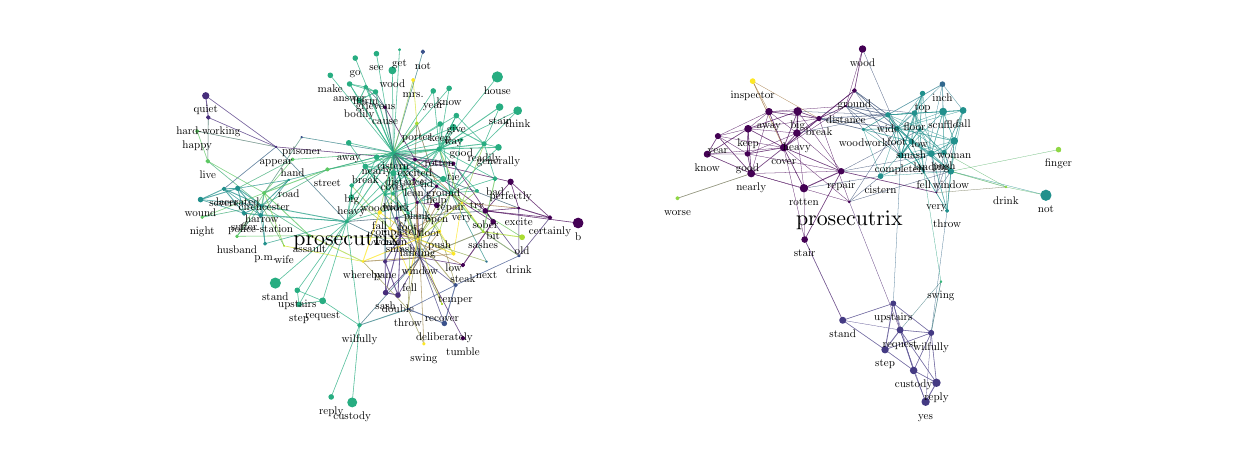
\begin{tikzpicture}[x=1pt,y=1pt]
\definecolor{fillColor}{RGB}{255,255,255}
\path[use as bounding box,fill=fillColor,fill opacity=0.00] (0,0) rectangle (433.62,144.54);
\begin{scope}
\path[clip] (  0.00,  0.00) rectangle (433.62,144.54);
\definecolor{drawColor}{RGB}{49,127,133}

\path[draw=drawColor,draw opacity=0.50,line width= 0.2pt,line join=round,line cap=round] (132.13, 99.35) -- (142.80,135.82);

\path[draw=drawColor,draw opacity=0.50,line width= 0.2pt,line join=round,line cap=round] (132.13, 99.35) -- ( 99.01,104.96);
\definecolor{drawColor}{RGB}{76,141,119}

\path[draw=drawColor,draw opacity=0.50,line width= 0.2pt,line join=round,line cap=round] ( 85.48, 84.82) -- ( 99.01,104.96);
\definecolor{drawColor}{RGB}{39,173,129}

\path[draw=drawColor,draw opacity=0.50,line width= 0.2pt,line join=round,line cap=round] (132.13, 99.35) -- (118.36,133.55);

\path[draw=drawColor,draw opacity=0.50,line width= 0.2pt,line join=round,line cap=round] (132.13, 99.35) -- (126.03,135.13);

\path[draw=drawColor,draw opacity=0.50,line width= 0.2pt,line join=round,line cap=round] (132.13, 99.35) -- (152.29,122.63);

\path[draw=drawColor,draw opacity=0.50,line width= 0.2pt,line join=round,line cap=round] (148.74,100.69) -- (152.29,122.63);

\path[draw=drawColor,draw opacity=0.50,line width= 0.2pt,line join=round,line cap=round] (144.25, 93.14) -- (154.91,112.76);

\path[draw=drawColor,draw opacity=0.50,line width= 0.2pt,line join=round,line cap=round] (164.94,102.57) -- (154.91,112.76);

\path[draw=drawColor,draw opacity=0.50,line width= 0.2pt,line join=round,line cap=round] (132.13, 99.35) -- (154.91,112.76);

\path[draw=drawColor,draw opacity=0.50,line width= 0.2pt,line join=round,line cap=round] (148.74,100.69) -- (154.91,112.76);

\path[draw=drawColor,draw opacity=0.50,line width= 0.2pt,line join=round,line cap=round] (132.13, 99.35) -- (134.37,136.59);

\path[draw=drawColor,draw opacity=0.50,line width= 0.2pt,line join=round,line cap=round] (148.74,100.69) -- (169.72,126.74);

\path[draw=drawColor,draw opacity=0.50,line width= 0.2pt,line join=round,line cap=round] (132.13, 99.35) -- (109.35,127.33);
\definecolor{drawColor}{RGB}{63,172,119}

\path[draw=drawColor,draw opacity=0.50,line width= 0.2pt,line join=round,line cap=round] ( 84.62, 80.23) -- ( 65.10, 96.31);
\definecolor{drawColor}{RGB}{93,200,99}

\path[draw=drawColor,draw opacity=0.50,line width= 0.2pt,line join=round,line cap=round] ( 61.26,107.12) -- ( 65.10, 96.31);
\definecolor{drawColor}{RGB}{81,122,111}

\path[draw=drawColor,draw opacity=0.50,line width= 0.2pt,line join=round,line cap=round] ( 65.27,112.09) -- ( 65.10, 96.31);
\definecolor{drawColor}{RGB}{93,200,99}

\path[draw=drawColor,draw opacity=0.50,line width= 0.2pt,line join=round,line cap=round] ( 85.48, 84.82) -- ( 65.10, 96.31);
\definecolor{drawColor}{RGB}{253,231,37}

\path[draw=drawColor,draw opacity=0.50,line width= 0.2pt,line join=round,line cap=round] (153.92, 62.85) -- (156.91, 81.26);
\definecolor{drawColor}{RGB}{146,202,83}

\path[draw=drawColor,draw opacity=0.50,line width= 0.2pt,line join=round,line cap=round] (152.90, 84.88) -- (156.91, 81.26);
\definecolor{drawColor}{RGB}{253,231,37}

\path[draw=drawColor,draw opacity=0.50,line width= 0.2pt,line join=round,line cap=round] (140.96, 68.17) -- (156.91, 81.26);
\definecolor{drawColor}{RGB}{160,116,60}

\path[draw=drawColor,draw opacity=0.50,line width= 0.2pt,line join=round,line cap=round] (139.94, 96.93) -- (156.91, 81.26);

\path[draw=drawColor,draw opacity=0.50,line width= 0.2pt,line join=round,line cap=round] (177.45, 79.33) -- (156.91, 81.26);
\definecolor{drawColor}{RGB}{162,138,80}

\path[draw=drawColor,draw opacity=0.50,line width= 0.2pt,line join=round,line cap=round] (134.78, 69.46) -- (156.91, 81.26);
\definecolor{drawColor}{RGB}{146,202,83}

\path[draw=drawColor,draw opacity=0.50,line width= 0.2pt,line join=round,line cap=round] (164.94,102.57) -- (156.91, 81.26);

\path[draw=drawColor,draw opacity=0.50,line width= 0.3pt,line join=round,line cap=round] (148.74,100.69) -- (156.91, 81.26);
\definecolor{drawColor}{RGB}{211,225,43}

\path[draw=drawColor,draw opacity=0.50,line width= 0.3pt,line join=round,line cap=round] (164.61, 70.80) -- (156.91, 81.26);
\definecolor{drawColor}{RGB}{39,173,129}

\path[draw=drawColor,draw opacity=0.50,line width= 0.2pt,line join=round,line cap=round] (164.94,102.57) -- (177.07,114.54);

\path[draw=drawColor,draw opacity=0.50,line width= 0.2pt,line join=round,line cap=round] (148.74,100.69) -- (177.07,114.54);

\path[draw=drawColor,draw opacity=0.50,line width= 0.2pt,line join=round,line cap=round] (132.13, 99.35) -- (146.55,121.67);

\path[draw=drawColor,draw opacity=0.50,line width= 0.2pt,line join=round,line cap=round] (148.74,100.69) -- (146.55,121.67);
\definecolor{drawColor}{RGB}{65,186,113}

\path[draw=drawColor,draw opacity=0.50,line width= 0.2pt,line join=round,line cap=round] (132.13, 99.35) -- ( 95.73, 96.94);
\definecolor{drawColor}{RGB}{63,172,119}

\path[draw=drawColor,draw opacity=0.50,line width= 0.2pt,line join=round,line cap=round] ( 75.88, 86.48) -- ( 95.73, 96.94);
\definecolor{drawColor}{RGB}{93,200,99}

\path[draw=drawColor,draw opacity=0.50,line width= 0.2pt,line join=round,line cap=round] ( 85.48, 84.82) -- ( 95.73, 96.94);
\definecolor{drawColor}{RGB}{63,172,119}

\path[draw=drawColor,draw opacity=0.50,line width= 0.2pt,line join=round,line cap=round] ( 84.62, 80.23) -- (108.33, 93.32);
\definecolor{drawColor}{RGB}{65,186,113}

\path[draw=drawColor,draw opacity=0.50,line width= 0.2pt,line join=round,line cap=round] (132.13, 99.35) -- (108.33, 93.32);

\path[draw=drawColor,draw opacity=0.50,line width= 0.2pt,line join=round,line cap=round] (148.74,100.69) -- (108.33, 93.32);
\definecolor{drawColor}{RGB}{93,200,99}

\path[draw=drawColor,draw opacity=0.50,line width= 0.3pt,line join=round,line cap=round] ( 85.48, 84.82) -- (108.33, 93.32);
\definecolor{drawColor}{RGB}{39,173,129}

\path[draw=drawColor,draw opacity=0.50,line width= 0.2pt,line join=round,line cap=round] (132.13, 99.35) -- (116.02,102.93);

\path[draw=drawColor,draw opacity=0.50,line width= 0.2pt,line join=round,line cap=round] (129.16, 84.26) -- (116.02,102.93);
\definecolor{drawColor}{RGB}{63,172,119}

\path[draw=drawColor,draw opacity=0.50,line width= 0.2pt,line join=round,line cap=round] ( 84.62, 80.23) -- ( 63.07, 76.03);
\definecolor{drawColor}{RGB}{93,200,99}

\path[draw=drawColor,draw opacity=0.50,line width= 0.2pt,line join=round,line cap=round] ( 85.48, 84.82) -- ( 63.07, 76.03);
\definecolor{drawColor}{RGB}{211,225,43}

\path[draw=drawColor,draw opacity=0.50,line width= 0.2pt,line join=round,line cap=round] (140.64,109.98) -- (139.30,125.62);
\definecolor{drawColor}{RGB}{146,202,83}

\path[draw=drawColor,draw opacity=0.50,line width= 0.2pt,line join=round,line cap=round] (132.13, 99.35) -- (139.30,125.62);
\definecolor{drawColor}{RGB}{160,116,60}

\path[draw=drawColor,draw opacity=0.50,line width= 0.2pt,line join=round,line cap=round] (140.96, 68.17) -- (147.86, 80.38);
\definecolor{drawColor}{RGB}{68,1,84}

\path[draw=drawColor,draw opacity=0.50,line width= 0.2pt,line join=round,line cap=round] (140.75, 81.38) -- (147.86, 80.38);
\definecolor{drawColor}{RGB}{53,87,106}

\path[draw=drawColor,draw opacity=0.50,line width= 0.2pt,line join=round,line cap=round] (132.13, 99.35) -- (147.86, 80.38);
\definecolor{drawColor}{RGB}{101,182,95}

\path[draw=drawColor,draw opacity=0.50,line width= 0.2pt,line join=round,line cap=round] ( 84.62, 80.23) -- ( 92.65, 65.70);
\definecolor{drawColor}{RGB}{211,225,43}

\path[draw=drawColor,draw opacity=0.50,line width= 0.2pt,line join=round,line cap=round] (121.14, 60.04) -- ( 92.65, 65.70);
\definecolor{drawColor}{RGB}{131,210,74}

\path[draw=drawColor,draw opacity=0.50,line width= 0.2pt,line join=round,line cap=round] ( 85.48, 84.82) -- ( 92.65, 65.70);
\definecolor{drawColor}{RGB}{39,173,129}

\path[draw=drawColor,draw opacity=0.50,line width= 0.2pt,line join=round,line cap=round] (152.90, 84.88) -- (149.05,109.73);

\path[draw=drawColor,draw opacity=0.50,line width= 0.2pt,line join=round,line cap=round] (132.13, 99.35) -- (149.05,109.73);

\path[draw=drawColor,draw opacity=0.50,line width= 0.2pt,line join=round,line cap=round] (148.74,100.69) -- (149.05,109.73);
\definecolor{drawColor}{RGB}{146,202,83}

\path[draw=drawColor,draw opacity=0.50,line width= 0.2pt,line join=round,line cap=round] (116.97, 83.29) -- (130.95, 72.00);

\path[draw=drawColor,draw opacity=0.50,line width= 0.2pt,line join=round,line cap=round] (117.08, 87.48) -- (130.95, 72.00);
\definecolor{drawColor}{RGB}{253,231,37}

\path[draw=drawColor,draw opacity=0.50,line width= 0.2pt,line join=round,line cap=round] (140.96, 68.17) -- (130.95, 72.00);
\definecolor{drawColor}{RGB}{162,138,80}

\path[draw=drawColor,draw opacity=0.50,line width= 0.2pt,line join=round,line cap=round] (134.78, 69.46) -- (130.95, 72.00);

\path[draw=drawColor,draw opacity=0.50,line width= 0.2pt,line join=round,line cap=round] (133.37, 75.71) -- (130.95, 72.00);
\definecolor{drawColor}{RGB}{253,231,37}

\path[draw=drawColor,draw opacity=0.50,line width= 0.2pt,line join=round,line cap=round] (138.04, 55.31) -- (130.95, 72.00);
\definecolor{drawColor}{RGB}{160,116,60}

\path[draw=drawColor,draw opacity=0.50,line width= 0.2pt,line join=round,line cap=round] (157.27, 58.77) -- (130.95, 72.00);
\definecolor{drawColor}{RGB}{146,202,83}

\path[draw=drawColor,draw opacity=0.50,line width= 0.2pt,line join=round,line cap=round] (132.13, 99.35) -- (130.95, 72.00);
\definecolor{drawColor}{RGB}{33,144,140}

\path[draw=drawColor,draw opacity=0.50,line width= 0.2pt,line join=round,line cap=round] ( 84.18, 76.72) -- ( 94.32, 89.54);

\path[draw=drawColor,draw opacity=0.50,line width= 0.3pt,line join=round,line cap=round] ( 84.62, 80.23) -- ( 94.32, 89.54);
\definecolor{drawColor}{RGB}{36,158,134}

\path[draw=drawColor,draw opacity=0.50,line width= 0.2pt,line join=round,line cap=round] (132.13, 99.35) -- ( 94.32, 89.54);
\definecolor{drawColor}{RGB}{33,144,140}

\path[draw=drawColor,draw opacity=0.50,line width= 0.2pt,line join=round,line cap=round] ( 75.88, 86.48) -- ( 94.32, 89.54);
\definecolor{drawColor}{RGB}{63,172,119}

\path[draw=drawColor,draw opacity=0.50,line width= 0.3pt,line join=round,line cap=round] ( 85.48, 84.82) -- ( 94.32, 89.54);
\definecolor{drawColor}{RGB}{39,173,129}

\path[draw=drawColor,draw opacity=0.50,line width= 0.2pt,line join=round,line cap=round] (152.90, 84.88) -- (156.66,104.05);

\path[draw=drawColor,draw opacity=0.50,line width= 0.2pt,line join=round,line cap=round] (132.13, 99.35) -- (156.66,104.05);

\path[draw=drawColor,draw opacity=0.50,line width= 0.2pt,line join=round,line cap=round] (148.74,100.69) -- (156.66,104.05);
\definecolor{drawColor}{RGB}{41,143,135}

\path[draw=drawColor,draw opacity=0.50,line width= 0.2pt,line join=round,line cap=round] (152.90, 84.88) -- (165.81, 60.02);
\definecolor{drawColor}{RGB}{148,172,89}

\path[draw=drawColor,draw opacity=0.50,line width= 0.2pt,line join=round,line cap=round] (140.96, 68.17) -- (165.81, 60.02);
\definecolor{drawColor}{RGB}{39,173,129}

\path[draw=drawColor,draw opacity=0.50,line width= 0.2pt,line join=round,line cap=round] (119.91, 37.03) -- (117.27,  9.13);

\path[draw=drawColor,draw opacity=0.50,line width= 0.2pt,line join=round,line cap=round] (144.25, 93.14) -- (153.83,108.51);

\path[draw=drawColor,draw opacity=0.50,line width= 0.3pt,line join=round,line cap=round] (164.94,102.57) -- (153.83,108.51);

\path[draw=drawColor,draw opacity=0.50,line width= 0.2pt,line join=round,line cap=round] (132.13, 99.35) -- (153.83,108.51);

\path[draw=drawColor,draw opacity=0.50,line width= 0.2pt,line join=round,line cap=round] (148.74,100.69) -- (153.83,108.51);

\path[draw=drawColor,draw opacity=0.50,line width= 0.2pt,line join=round,line cap=round] (115.27, 74.47) -- ( 89.50, 52.25);
\definecolor{drawColor}{RGB}{55,109,126}

\path[draw=drawColor,draw opacity=0.50,line width= 0.2pt,line join=round,line cap=round] (137.45, 77.39) -- (141.73, 61.49);

\path[draw=drawColor,draw opacity=0.50,line width= 0.2pt,line join=round,line cap=round] (115.27, 74.47) -- (141.73, 61.49);
\definecolor{drawColor}{RGB}{162,138,80}

\path[draw=drawColor,draw opacity=0.50,line width= 0.2pt,line join=round,line cap=round] (148.83, 70.95) -- (141.73, 61.49);
\definecolor{drawColor}{RGB}{120,132,86}

\path[draw=drawColor,draw opacity=0.50,line width= 0.2pt,line join=round,line cap=round] (149.71, 44.69) -- (141.73, 61.49);
\definecolor{drawColor}{RGB}{162,138,80}

\path[draw=drawColor,draw opacity=0.50,line width= 0.2pt,line join=round,line cap=round] (153.92, 62.85) -- (141.73, 61.49);
\definecolor{drawColor}{RGB}{71,45,123}

\path[draw=drawColor,draw opacity=0.50,line width= 0.2pt,line join=round,line cap=round] (133.81, 47.90) -- (141.73, 61.49);
\definecolor{drawColor}{RGB}{55,109,126}

\path[draw=drawColor,draw opacity=0.50,line width= 0.2pt,line join=round,line cap=round] (152.90, 84.88) -- (141.73, 61.49);
\definecolor{drawColor}{RGB}{71,45,123}

\path[draw=drawColor,draw opacity=0.50,line width= 0.2pt,line join=round,line cap=round] (129.34, 48.77) -- (141.73, 61.49);
\definecolor{drawColor}{RGB}{162,138,80}

\path[draw=drawColor,draw opacity=0.50,line width= 0.3pt,line join=round,line cap=round] (140.96, 68.17) -- (141.73, 61.49);
\definecolor{drawColor}{RGB}{71,45,123}

\path[draw=drawColor,draw opacity=0.50,line width= 0.2pt,line join=round,line cap=round] (129.17, 60.04) -- (141.73, 61.49);

\path[draw=drawColor,draw opacity=0.50,line width= 0.2pt,line join=round,line cap=round] (134.78, 69.46) -- (141.73, 61.49);
\definecolor{drawColor}{RGB}{55,109,126}

\path[draw=drawColor,draw opacity=0.50,line width= 0.2pt,line join=round,line cap=round] (144.25, 93.14) -- (141.73, 61.49);
\definecolor{drawColor}{RGB}{71,45,123}

\path[draw=drawColor,draw opacity=0.50,line width= 0.2pt,line join=round,line cap=round] (133.37, 75.71) -- (141.73, 61.49);
\definecolor{drawColor}{RGB}{69,23,103}

\path[draw=drawColor,draw opacity=0.50,line width= 0.2pt,line join=round,line cap=round] (140.75, 81.38) -- (141.73, 61.49);

\path[draw=drawColor,draw opacity=0.50,line width= 0.2pt,line join=round,line cap=round] (157.29, 32.32) -- (141.73, 61.49);
\definecolor{drawColor}{RGB}{162,138,80}

\path[draw=drawColor,draw opacity=0.50,line width= 0.2pt,line join=round,line cap=round] (138.04, 55.31) -- (141.73, 61.49);
\definecolor{drawColor}{RGB}{55,109,126}

\path[draw=drawColor,draw opacity=0.50,line width= 0.2pt,line join=round,line cap=round] (119.91, 37.03) -- (141.73, 61.49);
\definecolor{drawColor}{RGB}{65,63,131}

\path[draw=drawColor,draw opacity=0.50,line width= 0.2pt,line join=round,line cap=round] (154.60, 51.52) -- (141.73, 61.49);
\definecolor{drawColor}{RGB}{162,138,80}

\path[draw=drawColor,draw opacity=0.50,line width= 0.2pt,line join=round,line cap=round] (143.17, 30.30) -- (141.73, 61.49);
\definecolor{drawColor}{RGB}{65,63,131}

\path[draw=drawColor,draw opacity=0.50,line width= 0.2pt,line join=round,line cap=round] (150.57, 37.67) -- (141.73, 61.49);
\definecolor{drawColor}{RGB}{69,23,103}

\path[draw=drawColor,draw opacity=0.50,line width= 0.2pt,line join=round,line cap=round] (157.27, 58.77) -- (141.73, 61.49);
\definecolor{drawColor}{RGB}{55,109,126}

\path[draw=drawColor,draw opacity=0.50,line width= 0.3pt,line join=round,line cap=round] (132.13, 99.35) -- (141.73, 61.49);
\definecolor{drawColor}{RGB}{162,138,80}

\path[draw=drawColor,draw opacity=0.50,line width= 0.3pt,line join=round,line cap=round] (121.14, 60.04) -- (141.73, 61.49);
\definecolor{drawColor}{RGB}{120,132,86}

\path[draw=drawColor,draw opacity=0.50,line width= 0.3pt,line join=round,line cap=round] (164.61, 70.80) -- (141.73, 61.49);
\definecolor{drawColor}{RGB}{39,173,129}

\path[draw=drawColor,draw opacity=0.50,line width= 0.2pt,line join=round,line cap=round] (152.90, 84.88) -- (168.88, 89.98);

\path[draw=drawColor,draw opacity=0.50,line width= 0.2pt,line join=round,line cap=round] (164.94,102.57) -- (168.88, 89.98);

\path[draw=drawColor,draw opacity=0.50,line width= 0.2pt,line join=round,line cap=round] (148.74,100.69) -- (168.88, 89.98);
\definecolor{drawColor}{RGB}{104,196,89}

\path[draw=drawColor,draw opacity=0.50,line width= 0.3pt,line join=round,line cap=round] (164.61, 70.80) -- (168.88, 89.98);
\definecolor{drawColor}{RGB}{39,173,129}

\path[draw=drawColor,draw opacity=0.50,line width= 0.2pt,line join=round,line cap=round] (132.11, 91.99) -- (122.00, 94.41);

\path[draw=drawColor,draw opacity=0.50,line width= 0.2pt,line join=round,line cap=round] (136.33, 93.67) -- (122.00, 94.41);

\path[draw=drawColor,draw opacity=0.50,line width= 0.2pt,line join=round,line cap=round] (132.08, 84.53) -- (122.00, 94.41);

\path[draw=drawColor,draw opacity=0.50,line width= 0.2pt,line join=round,line cap=round] (117.08, 87.48) -- (122.00, 94.41);

\path[draw=drawColor,draw opacity=0.50,line width= 0.3pt,line join=round,line cap=round] (132.13, 99.35) -- (122.00, 94.41);

\path[draw=drawColor,draw opacity=0.50,line width= 0.3pt,line join=round,line cap=round] (129.16, 84.26) -- (122.00, 94.41);
\definecolor{drawColor}{RGB}{55,109,126}

\path[draw=drawColor,draw opacity=0.50,line width= 0.2pt,line join=round,line cap=round] (115.27, 74.47) -- ( 89.75,101.46);
\definecolor{drawColor}{RGB}{71,45,123}

\path[draw=drawColor,draw opacity=0.50,line width= 0.2pt,line join=round,line cap=round] ( 64.34,119.94) -- ( 89.75,101.46);
\definecolor{drawColor}{RGB}{52,94,131}

\path[draw=drawColor,draw opacity=0.50,line width= 0.2pt,line join=round,line cap=round] ( 70.92, 86.30) -- ( 89.75,101.46);
\definecolor{drawColor}{RGB}{69,23,103}

\path[draw=drawColor,draw opacity=0.50,line width= 0.2pt,line join=round,line cap=round] (139.94, 96.93) -- ( 89.75,101.46);
\definecolor{drawColor}{RGB}{81,122,111}

\path[draw=drawColor,draw opacity=0.50,line width= 0.2pt,line join=round,line cap=round] ( 61.26,107.12) -- ( 89.75,101.46);
\definecolor{drawColor}{RGB}{71,45,123}

\path[draw=drawColor,draw opacity=0.50,line width= 0.2pt,line join=round,line cap=round] ( 65.27,112.09) -- ( 89.75,101.46);
\definecolor{drawColor}{RGB}{93,200,99}

\path[draw=drawColor,draw opacity=0.50,line width= 0.2pt,line join=round,line cap=round] (101.88, 69.39) -- ( 75.63, 69.15);
\definecolor{drawColor}{RGB}{63,172,119}

\path[draw=drawColor,draw opacity=0.50,line width= 0.2pt,line join=round,line cap=round] ( 84.62, 80.23) -- ( 75.63, 69.15);
\definecolor{drawColor}{RGB}{93,200,99}

\path[draw=drawColor,draw opacity=0.50,line width= 0.2pt,line join=round,line cap=round] ( 85.48, 84.82) -- ( 75.63, 69.15);
\definecolor{drawColor}{RGB}{39,173,129}

\path[draw=drawColor,draw opacity=0.50,line width= 0.2pt,line join=round,line cap=round] (152.90, 84.88) -- (162.38, 85.56);
\definecolor{drawColor}{RGB}{146,202,82}

\path[draw=drawColor,draw opacity=0.50,line width= 0.2pt,line join=round,line cap=round] (140.96, 68.17) -- (162.38, 85.56);
\definecolor{drawColor}{RGB}{39,173,129}

\path[draw=drawColor,draw opacity=0.50,line width= 0.2pt,line join=round,line cap=round] (148.74,100.69) -- (162.38, 85.56);
\definecolor{drawColor}{RGB}{104,196,89}

\path[draw=drawColor,draw opacity=0.50,line width= 0.2pt,line join=round,line cap=round] (152.90, 84.88) -- (178.66, 68.81);
\definecolor{drawColor}{RGB}{170,220,50}

\path[draw=drawColor,draw opacity=0.50,line width= 0.3pt,line join=round,line cap=round] (164.61, 70.80) -- (178.66, 68.81);
\definecolor{drawColor}{RGB}{39,173,129}

\path[draw=drawColor,draw opacity=0.50,line width= 0.2pt,line join=round,line cap=round] (164.94,102.57) -- (170.53,115.85);

\path[draw=drawColor,draw opacity=0.50,line width= 0.3pt,line join=round,line cap=round] (148.74,100.69) -- (170.53,115.85);
\definecolor{drawColor}{RGB}{63,41,111}

\path[draw=drawColor,draw opacity=0.50,line width= 0.2pt,line join=round,line cap=round] (165.38, 78.34) -- (177.53, 62.09);

\path[draw=drawColor,draw opacity=0.50,line width= 0.2pt,line join=round,line cap=round] (188.75, 75.90) -- (177.53, 62.09);

\path[draw=drawColor,draw opacity=0.50,line width= 0.2pt,line join=round,line cap=round] (177.45, 79.33) -- (177.53, 62.09);
\definecolor{drawColor}{RGB}{59,82,139}

\path[draw=drawColor,draw opacity=0.50,line width= 0.2pt,line join=round,line cap=round] (154.60, 51.52) -- (177.53, 62.09);
\definecolor{drawColor}{RGB}{114,151,94}

\path[draw=drawColor,draw opacity=0.50,line width= 0.3pt,line join=round,line cap=round] (164.61, 70.80) -- (177.53, 62.09);
\definecolor{drawColor}{RGB}{156,156,88}

\path[draw=drawColor,draw opacity=0.50,line width= 0.2pt,line join=round,line cap=round] (140.96, 68.17) -- (137.40, 42.87);

\path[draw=drawColor,draw opacity=0.50,line width= 0.2pt,line join=round,line cap=round] (138.04, 55.31) -- (137.40, 42.87);
\definecolor{drawColor}{RGB}{49,127,133}

\path[draw=drawColor,draw opacity=0.50,line width= 0.3pt,line join=round,line cap=round] (119.91, 37.03) -- (137.40, 42.87);
\definecolor{drawColor}{RGB}{59,82,139}

\path[draw=drawColor,draw opacity=0.50,line width= 0.2pt,line join=round,line cap=round] (154.60, 51.52) -- (137.40, 42.87);
\definecolor{drawColor}{RGB}{156,156,88}

\path[draw=drawColor,draw opacity=0.50,line width= 0.2pt,line join=round,line cap=round] (143.17, 30.30) -- (137.40, 42.87);
\definecolor{drawColor}{RGB}{59,82,139}

\path[draw=drawColor,draw opacity=0.50,line width= 0.3pt,line join=round,line cap=round] (150.57, 37.67) -- (137.40, 42.87);
\definecolor{drawColor}{RGB}{156,156,88}

\path[draw=drawColor,draw opacity=0.50,line width= 0.2pt,line join=round,line cap=round] (121.14, 60.04) -- (137.40, 42.87);
\definecolor{drawColor}{RGB}{146,202,83}

\path[draw=drawColor,draw opacity=0.50,line width= 0.2pt,line join=round,line cap=round] (132.08, 84.53) -- (127.19, 77.78);
\definecolor{drawColor}{RGB}{253,231,37}

\path[draw=drawColor,draw opacity=0.50,line width= 0.2pt,line join=round,line cap=round] (140.96, 68.17) -- (127.19, 77.78);
\definecolor{drawColor}{RGB}{146,202,83}

\path[draw=drawColor,draw opacity=0.50,line width= 0.2pt,line join=round,line cap=round] (144.25, 93.14) -- (127.19, 77.78);

\path[draw=drawColor,draw opacity=0.50,line width= 0.2pt,line join=round,line cap=round] (132.13, 99.35) -- (127.19, 77.78);
\definecolor{drawColor}{RGB}{253,231,37}

\path[draw=drawColor,draw opacity=0.50,line width= 0.3pt,line join=round,line cap=round] (121.14, 60.04) -- (127.19, 77.78);
\definecolor{drawColor}{RGB}{39,173,129}

\path[draw=drawColor,draw opacity=0.50,line width= 0.2pt,line join=round,line cap=round] (122.14,123.13) -- (116.32,124.20);

\path[draw=drawColor,draw opacity=0.50,line width= 0.2pt,line join=round,line cap=round] (119.79,118.23) -- (116.32,124.20);

\path[draw=drawColor,draw opacity=0.50,line width= 0.2pt,line join=round,line cap=round] (125.70,121.33) -- (116.32,124.20);

\path[draw=drawColor,draw opacity=0.50,line width= 0.2pt,line join=round,line cap=round] (132.13, 99.35) -- (116.32,124.20);
\definecolor{drawColor}{RGB}{33,144,140}

\path[draw=drawColor,draw opacity=0.50,line width= 0.2pt,line join=round,line cap=round] ( 78.20, 77.48) -- ( 62.47, 82.42);

\path[draw=drawColor,draw opacity=0.50,line width= 0.3pt,line join=round,line cap=round] ( 70.92, 86.30) -- ( 62.47, 82.42);

\path[draw=drawColor,draw opacity=0.50,line width= 0.2pt,line join=round,line cap=round] ( 84.62, 80.23) -- ( 62.47, 82.42);

\path[draw=drawColor,draw opacity=0.50,line width= 0.3pt,line join=round,line cap=round] ( 75.88, 86.48) -- ( 62.47, 82.42);
\definecolor{drawColor}{RGB}{39,173,129}

\path[draw=drawColor,draw opacity=0.50,line width= 0.2pt,line join=round,line cap=round] (137.45, 77.39) -- (150.17, 89.86);

\path[draw=drawColor,draw opacity=0.50,line width= 0.2pt,line join=round,line cap=round] (136.33, 93.67) -- (150.17, 89.86);
\definecolor{drawColor}{RGB}{53,87,106}

\path[draw=drawColor,draw opacity=0.50,line width= 0.2pt,line join=round,line cap=round] (177.45, 79.33) -- (150.17, 89.86);
\definecolor{drawColor}{RGB}{39,173,129}

\path[draw=drawColor,draw opacity=0.50,line width= 0.3pt,line join=round,line cap=round] (132.13, 99.35) -- (150.17, 89.86);

\path[draw=drawColor,draw opacity=0.50,line width= 0.3pt,line join=round,line cap=round] (129.16, 84.26) -- (150.17, 89.86);

\path[draw=drawColor,draw opacity=0.50,line width= 0.2pt,line join=round,line cap=round] (137.45, 77.39) -- (145.14, 75.40);
\definecolor{drawColor}{RGB}{146,202,82}

\path[draw=drawColor,draw opacity=0.50,line width= 0.2pt,line join=round,line cap=round] (153.92, 62.85) -- (145.14, 75.40);

\path[draw=drawColor,draw opacity=0.50,line width= 0.2pt,line join=round,line cap=round] (140.96, 68.17) -- (145.14, 75.40);
\definecolor{drawColor}{RGB}{39,173,129}

\path[draw=drawColor,draw opacity=0.50,line width= 0.2pt,line join=round,line cap=round] (132.13, 99.35) -- (145.14, 75.40);
\definecolor{drawColor}{RGB}{55,109,126}

\path[draw=drawColor,draw opacity=0.50,line width= 0.2pt,line join=round,line cap=round] (141.73, 61.49) -- (137.45, 77.39);
\definecolor{drawColor}{RGB}{39,173,129}

\path[draw=drawColor,draw opacity=0.50,line width= 0.2pt,line join=round,line cap=round] (150.17, 89.86) -- (137.45, 77.39);

\path[draw=drawColor,draw opacity=0.50,line width= 0.2pt,line join=round,line cap=round] (145.14, 75.40) -- (137.45, 77.39);

\path[draw=drawColor,draw opacity=0.50,line width= 0.2pt,line join=round,line cap=round] (136.33, 93.67) -- (137.45, 77.39);

\path[draw=drawColor,draw opacity=0.50,line width= 0.3pt,line join=round,line cap=round] (132.08, 84.53) -- (137.45, 77.39);
\definecolor{drawColor}{RGB}{146,202,82}

\path[draw=drawColor,draw opacity=0.50,line width= 0.3pt,line join=round,line cap=round] (140.96, 68.17) -- (137.45, 77.39);
\definecolor{drawColor}{RGB}{55,109,126}

\path[draw=drawColor,draw opacity=0.50,line width= 0.2pt,line join=round,line cap=round] (134.78, 69.46) -- (137.45, 77.39);

\path[draw=drawColor,draw opacity=0.50,line width= 0.2pt,line join=round,line cap=round] (133.37, 75.71) -- (137.45, 77.39);
\definecolor{drawColor}{RGB}{146,202,82}

\path[draw=drawColor,draw opacity=0.50,line width= 0.2pt,line join=round,line cap=round] (138.04, 55.31) -- (137.45, 77.39);
\definecolor{drawColor}{RGB}{39,173,129}

\path[draw=drawColor,draw opacity=0.50,line width= 0.3pt,line join=round,line cap=round] (132.13, 99.35) -- (137.45, 77.39);

\path[draw=drawColor,draw opacity=0.50,line width= 0.3pt,line join=round,line cap=round] (129.16, 84.26) -- (137.45, 77.39);

\path[draw=drawColor,draw opacity=0.50,line width= 0.2pt,line join=round,line cap=round] (132.13, 99.35) -- (131.79,129.11);
\definecolor{drawColor}{RGB}{53,87,106}

\path[draw=drawColor,draw opacity=0.50,line width= 0.2pt,line join=round,line cap=round] (122.14,123.13) -- (129.12,115.76);

\path[draw=drawColor,draw opacity=0.50,line width= 0.2pt,line join=round,line cap=round] (119.79,118.23) -- (129.12,115.76);

\path[draw=drawColor,draw opacity=0.50,line width= 0.2pt,line join=round,line cap=round] (125.70,121.33) -- (129.12,115.76);
\definecolor{drawColor}{RGB}{68,1,84}

\path[draw=drawColor,draw opacity=0.50,line width= 0.2pt,line join=round,line cap=round] (139.94, 96.93) -- (129.12,115.76);
\definecolor{drawColor}{RGB}{53,87,106}

\path[draw=drawColor,draw opacity=0.50,line width= 0.3pt,line join=round,line cap=round] (132.13, 99.35) -- (129.12,115.76);
\definecolor{drawColor}{RGB}{211,225,43}

\path[draw=drawColor,draw opacity=0.50,line width= 0.2pt,line join=round,line cap=round] (139.30,125.62) -- (140.64,109.98);
\definecolor{drawColor}{RGB}{119,110,67}

\path[draw=drawColor,draw opacity=0.50,line width= 0.2pt,line join=round,line cap=round] (147.78, 87.27) -- (140.64,109.98);

\path[draw=drawColor,draw opacity=0.50,line width= 0.2pt,line join=round,line cap=round] (139.57, 89.71) -- (140.64,109.98);
\definecolor{drawColor}{RGB}{104,196,89}

\path[draw=drawColor,draw opacity=0.50,line width= 0.3pt,line join=round,line cap=round] (132.13, 99.35) -- (140.64,109.98);
\definecolor{drawColor}{RGB}{39,173,129}

\path[draw=drawColor,draw opacity=0.50,line width= 0.2pt,line join=round,line cap=round] (119.91, 37.03) -- (109.68, 11.10);
\definecolor{drawColor}{RGB}{93,200,99}

\path[draw=drawColor,draw opacity=0.50,line width= 0.2pt,line join=round,line cap=round] ( 75.63, 69.15) -- (101.88, 69.39);
\definecolor{drawColor}{RGB}{173,215,68}

\path[draw=drawColor,draw opacity=0.50,line width= 0.2pt,line join=round,line cap=round] (140.96, 68.17) -- (101.88, 69.39);
\definecolor{drawColor}{RGB}{63,172,119}

\path[draw=drawColor,draw opacity=0.50,line width= 0.2pt,line join=round,line cap=round] ( 84.62, 80.23) -- (101.88, 69.39);
\definecolor{drawColor}{RGB}{173,215,68}

\path[draw=drawColor,draw opacity=0.50,line width= 0.3pt,line join=round,line cap=round] (121.14, 60.04) -- (101.88, 69.39);
\definecolor{drawColor}{RGB}{93,200,99}

\path[draw=drawColor,draw opacity=0.50,line width= 0.3pt,line join=round,line cap=round] ( 85.48, 84.82) -- (101.88, 69.39);
\definecolor{drawColor}{RGB}{63,41,111}

\path[draw=drawColor,draw opacity=0.50,line width= 0.2pt,line join=round,line cap=round] (177.53, 62.09) -- (165.38, 78.34);
\definecolor{drawColor}{RGB}{53,87,106}

\path[draw=drawColor,draw opacity=0.50,line width= 0.2pt,line join=round,line cap=round] (115.27, 74.47) -- (165.38, 78.34);
\definecolor{drawColor}{RGB}{68,1,84}

\path[draw=drawColor,draw opacity=0.50,line width= 0.2pt,line join=round,line cap=round] (198.91, 73.96) -- (165.38, 78.34);

\path[draw=drawColor,draw opacity=0.50,line width= 0.2pt,line join=round,line cap=round] (174.50, 88.85) -- (165.38, 78.34);

\path[draw=drawColor,draw opacity=0.50,line width= 0.2pt,line join=round,line cap=round] (188.75, 75.90) -- (165.38, 78.34);

\path[draw=drawColor,draw opacity=0.50,line width= 0.2pt,line join=round,line cap=round] (168.22, 74.38) -- (165.38, 78.34);

\path[draw=drawColor,draw opacity=0.50,line width= 0.2pt,line join=round,line cap=round] (139.94, 96.93) -- (165.38, 78.34);

\path[draw=drawColor,draw opacity=0.50,line width= 0.2pt,line join=round,line cap=round] (177.45, 79.33) -- (165.38, 78.34);
\definecolor{drawColor}{RGB}{39,173,129}

\path[draw=drawColor,draw opacity=0.50,line width= 0.2pt,line join=round,line cap=round] ( 89.50, 52.25) -- (115.27, 74.47);
\definecolor{drawColor}{RGB}{55,109,126}

\path[draw=drawColor,draw opacity=0.50,line width= 0.2pt,line join=round,line cap=round] (141.73, 61.49) -- (115.27, 74.47);

\path[draw=drawColor,draw opacity=0.50,line width= 0.2pt,line join=round,line cap=round] ( 89.75,101.46) -- (115.27, 74.47);
\definecolor{drawColor}{RGB}{53,87,106}

\path[draw=drawColor,draw opacity=0.50,line width= 0.2pt,line join=round,line cap=round] (165.38, 78.34) -- (115.27, 74.47);
\definecolor{drawColor}{RGB}{39,173,129}

\path[draw=drawColor,draw opacity=0.50,line width= 0.2pt,line join=round,line cap=round] (126.11, 97.73) -- (115.27, 74.47);

\path[draw=drawColor,draw opacity=0.50,line width= 0.2pt,line join=round,line cap=round] ( 98.06, 44.55) -- (115.27, 74.47);
\definecolor{drawColor}{RGB}{36,158,134}

\path[draw=drawColor,draw opacity=0.50,line width= 0.2pt,line join=round,line cap=round] ( 85.79, 66.49) -- (115.27, 74.47);
\definecolor{drawColor}{RGB}{39,173,129}

\path[draw=drawColor,draw opacity=0.50,line width= 0.2pt,line join=round,line cap=round] (106.59, 45.84) -- (115.27, 74.47);

\path[draw=drawColor,draw opacity=0.50,line width= 0.2pt,line join=round,line cap=round] (132.11, 91.99) -- (115.27, 74.47);
\definecolor{drawColor}{RGB}{36,158,134}

\path[draw=drawColor,draw opacity=0.50,line width= 0.2pt,line join=round,line cap=round] ( 78.20, 77.48) -- (115.27, 74.47);
\definecolor{drawColor}{RGB}{39,173,129}

\path[draw=drawColor,draw opacity=0.50,line width= 0.2pt,line join=round,line cap=round] ( 97.42, 49.64) -- (115.27, 74.47);
\definecolor{drawColor}{RGB}{36,158,134}

\path[draw=drawColor,draw opacity=0.50,line width= 0.2pt,line join=round,line cap=round] ( 84.18, 76.72) -- (115.27, 74.47);
\definecolor{drawColor}{RGB}{39,173,129}

\path[draw=drawColor,draw opacity=0.50,line width= 0.2pt,line join=round,line cap=round] (152.90, 84.88) -- (115.27, 74.47);

\path[draw=drawColor,draw opacity=0.50,line width= 0.2pt,line join=round,line cap=round] (116.97, 83.29) -- (115.27, 74.47);

\path[draw=drawColor,draw opacity=0.50,line width= 0.2pt,line join=round,line cap=round] (117.08, 87.48) -- (115.27, 74.47);
\definecolor{drawColor}{RGB}{36,158,134}

\path[draw=drawColor,draw opacity=0.50,line width= 0.3pt,line join=round,line cap=round] ( 84.62, 80.23) -- (115.27, 74.47);
\definecolor{drawColor}{RGB}{39,173,129}

\path[draw=drawColor,draw opacity=0.50,line width= 0.2pt,line join=round,line cap=round] (119.91, 37.03) -- (115.27, 74.47);

\path[draw=drawColor,draw opacity=0.50,line width= 0.3pt,line join=round,line cap=round] (132.13, 99.35) -- (115.27, 74.47);

\path[draw=drawColor,draw opacity=0.50,line width= 0.3pt,line join=round,line cap=round] (148.74,100.69) -- (115.27, 74.47);

\path[draw=drawColor,draw opacity=0.50,line width= 0.2pt,line join=round,line cap=round] (115.27, 74.47) -- (126.11, 97.73);

\path[draw=drawColor,draw opacity=0.50,line width= 0.2pt,line join=round,line cap=round] (132.11, 91.99) -- (126.11, 97.73);

\path[draw=drawColor,draw opacity=0.50,line width= 0.2pt,line join=round,line cap=round] (132.13, 99.35) -- (126.11, 97.73);

\path[draw=drawColor,draw opacity=0.50,line width= 0.3pt,line join=round,line cap=round] (148.74,100.69) -- (126.11, 97.73);

\path[draw=drawColor,draw opacity=0.50,line width= 0.2pt,line join=round,line cap=round] (115.27, 74.47) -- ( 98.06, 44.55);

\path[draw=drawColor,draw opacity=0.50,line width= 0.2pt,line join=round,line cap=round] (106.59, 45.84) -- ( 98.06, 44.55);

\path[draw=drawColor,draw opacity=0.50,line width= 0.2pt,line join=round,line cap=round] ( 97.42, 49.64) -- ( 98.06, 44.55);
\definecolor{drawColor}{RGB}{119,110,67}

\path[draw=drawColor,draw opacity=0.50,line width= 0.2pt,line join=round,line cap=round] (140.64,109.98) -- (147.78, 87.27);
\definecolor{drawColor}{RGB}{68,1,84}

\path[draw=drawColor,draw opacity=0.50,line width= 0.2pt,line join=round,line cap=round] (168.22, 74.38) -- (147.78, 87.27);
\definecolor{drawColor}{RGB}{160,116,60}

\path[draw=drawColor,draw opacity=0.50,line width= 0.2pt,line join=round,line cap=round] (140.96, 68.17) -- (147.78, 87.27);
\definecolor{drawColor}{RGB}{68,1,84}

\path[draw=drawColor,draw opacity=0.50,line width= 0.2pt,line join=round,line cap=round] (140.75, 81.38) -- (147.78, 87.27);
\definecolor{drawColor}{RGB}{53,87,106}

\path[draw=drawColor,draw opacity=0.50,line width= 0.3pt,line join=round,line cap=round] (132.13, 99.35) -- (147.78, 87.27);
\definecolor{drawColor}{RGB}{36,158,134}

\path[draw=drawColor,draw opacity=0.50,line width= 0.2pt,line join=round,line cap=round] (115.27, 74.47) -- ( 85.79, 66.49);
\definecolor{drawColor}{RGB}{33,144,140}

\path[draw=drawColor,draw opacity=0.50,line width= 0.2pt,line join=round,line cap=round] ( 84.18, 76.72) -- ( 85.79, 66.49);

\path[draw=drawColor,draw opacity=0.50,line width= 0.2pt,line join=round,line cap=round] ( 84.62, 80.23) -- ( 85.79, 66.49);
\definecolor{drawColor}{RGB}{68,1,84}

\path[draw=drawColor,draw opacity=0.50,line width= 0.2pt,line join=round,line cap=round] (165.38, 78.34) -- (198.91, 73.96);
\definecolor{drawColor}{RGB}{162,138,80}

\path[draw=drawColor,draw opacity=0.50,line width= 0.2pt,line join=round,line cap=round] (141.73, 61.49) -- (148.83, 70.95);
\definecolor{drawColor}{RGB}{253,231,37}

\path[draw=drawColor,draw opacity=0.50,line width= 0.2pt,line join=round,line cap=round] (153.92, 62.85) -- (148.83, 70.95);
\definecolor{drawColor}{RGB}{146,202,83}

\path[draw=drawColor,draw opacity=0.50,line width= 0.2pt,line join=round,line cap=round] (152.90, 84.88) -- (148.83, 70.95);
\definecolor{drawColor}{RGB}{253,231,37}

\path[draw=drawColor,draw opacity=0.50,line width= 0.3pt,line join=round,line cap=round] (140.96, 68.17) -- (148.83, 70.95);
\definecolor{drawColor}{RGB}{156,156,88}

\path[draw=drawColor,draw opacity=0.50,line width= 0.2pt,line join=round,line cap=round] (154.60, 51.52) -- (148.83, 70.95);
\definecolor{drawColor}{RGB}{146,202,83}

\path[draw=drawColor,draw opacity=0.50,line width= 0.2pt,line join=round,line cap=round] (132.13, 99.35) -- (148.83, 70.95);
\definecolor{drawColor}{RGB}{68,1,84}

\path[draw=drawColor,draw opacity=0.50,line width= 0.2pt,line join=round,line cap=round] (165.38, 78.34) -- (174.50, 88.85);

\path[draw=drawColor,draw opacity=0.50,line width= 0.2pt,line join=round,line cap=round] (188.75, 75.90) -- (174.50, 88.85);

\path[draw=drawColor,draw opacity=0.50,line width= 0.2pt,line join=round,line cap=round] (139.94, 96.93) -- (174.50, 88.85);

\path[draw=drawColor,draw opacity=0.50,line width= 0.2pt,line join=round,line cap=round] (177.45, 79.33) -- (174.50, 88.85);
\definecolor{drawColor}{RGB}{63,41,111}

\path[draw=drawColor,draw opacity=0.50,line width= 0.2pt,line join=round,line cap=round] (177.53, 62.09) -- (188.75, 75.90);
\definecolor{drawColor}{RGB}{68,1,84}

\path[draw=drawColor,draw opacity=0.50,line width= 0.2pt,line join=round,line cap=round] (165.38, 78.34) -- (188.75, 75.90);

\path[draw=drawColor,draw opacity=0.50,line width= 0.2pt,line join=round,line cap=round] (174.50, 88.85) -- (188.75, 75.90);

\path[draw=drawColor,draw opacity=0.50,line width= 0.3pt,line join=round,line cap=round] (177.45, 79.33) -- (188.75, 75.90);
\definecolor{drawColor}{RGB}{39,173,129}

\path[draw=drawColor,draw opacity=0.50,line width= 0.2pt,line join=round,line cap=round] (152.90, 84.88) -- (170.12,101.29);

\path[draw=drawColor,draw opacity=0.50,line width= 0.2pt,line join=round,line cap=round] (164.94,102.57) -- (170.12,101.29);

\path[draw=drawColor,draw opacity=0.50,line width= 0.3pt,line join=round,line cap=round] (148.74,100.69) -- (170.12,101.29);

\path[draw=drawColor,draw opacity=0.50,line width= 0.2pt,line join=round,line cap=round] (115.27, 74.47) -- (106.59, 45.84);

\path[draw=drawColor,draw opacity=0.50,line width= 0.2pt,line join=round,line cap=round] ( 98.06, 44.55) -- (106.59, 45.84);

\path[draw=drawColor,draw opacity=0.50,line width= 0.2pt,line join=round,line cap=round] ( 97.42, 49.64) -- (106.59, 45.84);

\path[draw=drawColor,draw opacity=0.50,line width= 0.2pt,line join=round,line cap=round] (119.91, 37.03) -- (106.59, 45.84);
\definecolor{drawColor}{RGB}{68,1,84}

\path[draw=drawColor,draw opacity=0.50,line width= 0.2pt,line join=round,line cap=round] (168.22, 74.38) -- (153.84, 95.44);
\definecolor{drawColor}{RGB}{53,87,106}

\path[draw=drawColor,draw opacity=0.50,line width= 0.2pt,line join=round,line cap=round] (136.33, 93.67) -- (153.84, 95.44);
\definecolor{drawColor}{RGB}{68,1,84}

\path[draw=drawColor,draw opacity=0.50,line width= 0.3pt,line join=round,line cap=round] (139.94, 96.93) -- (153.84, 95.44);
\definecolor{drawColor}{RGB}{53,87,106}

\path[draw=drawColor,draw opacity=0.50,line width= 0.3pt,line join=round,line cap=round] (132.13, 99.35) -- (153.84, 95.44);
\definecolor{drawColor}{RGB}{39,173,129}

\path[draw=drawColor,draw opacity=0.50,line width= 0.2pt,line join=round,line cap=round] (122.00, 94.41) -- (132.11, 91.99);

\path[draw=drawColor,draw opacity=0.50,line width= 0.2pt,line join=round,line cap=round] (115.27, 74.47) -- (132.11, 91.99);

\path[draw=drawColor,draw opacity=0.50,line width= 0.2pt,line join=round,line cap=round] (126.11, 97.73) -- (132.11, 91.99);

\path[draw=drawColor,draw opacity=0.50,line width= 0.2pt,line join=round,line cap=round] (152.90, 84.88) -- (132.11, 91.99);

\path[draw=drawColor,draw opacity=0.50,line width= 0.3pt,line join=round,line cap=round] (132.13, 99.35) -- (132.11, 91.99);

\path[draw=drawColor,draw opacity=0.50,line width= 0.3pt,line join=round,line cap=round] (148.74,100.69) -- (132.11, 91.99);

\path[draw=drawColor,draw opacity=0.50,line width= 0.3pt,line join=round,line cap=round] (129.16, 84.26) -- (132.11, 91.99);
\definecolor{drawColor}{RGB}{68,1,84}

\path[draw=drawColor,draw opacity=0.50,line width= 0.2pt,line join=round,line cap=round] (165.38, 78.34) -- (168.22, 74.38);

\path[draw=drawColor,draw opacity=0.50,line width= 0.2pt,line join=round,line cap=round] (147.78, 87.27) -- (168.22, 74.38);

\path[draw=drawColor,draw opacity=0.50,line width= 0.2pt,line join=round,line cap=round] (153.84, 95.44) -- (168.22, 74.38);

\path[draw=drawColor,draw opacity=0.50,line width= 0.3pt,line join=round,line cap=round] (157.27, 58.77) -- (168.22, 74.38);
\definecolor{drawColor}{RGB}{39,173,129}

\path[draw=drawColor,draw opacity=0.50,line width= 0.2pt,line join=round,line cap=round] (122.00, 94.41) -- (136.33, 93.67);

\path[draw=drawColor,draw opacity=0.50,line width= 0.2pt,line join=round,line cap=round] (150.17, 89.86) -- (136.33, 93.67);

\path[draw=drawColor,draw opacity=0.50,line width= 0.2pt,line join=round,line cap=round] (137.45, 77.39) -- (136.33, 93.67);
\definecolor{drawColor}{RGB}{53,87,106}

\path[draw=drawColor,draw opacity=0.50,line width= 0.2pt,line join=round,line cap=round] (153.84, 95.44) -- (136.33, 93.67);
\definecolor{drawColor}{RGB}{39,173,129}

\path[draw=drawColor,draw opacity=0.50,line width= 0.2pt,line join=round,line cap=round] (132.08, 84.53) -- (136.33, 93.67);
\definecolor{drawColor}{RGB}{53,87,106}

\path[draw=drawColor,draw opacity=0.50,line width= 0.2pt,line join=round,line cap=round] (139.94, 96.93) -- (136.33, 93.67);
\definecolor{drawColor}{RGB}{39,173,129}

\path[draw=drawColor,draw opacity=0.50,line width= 0.3pt,line join=round,line cap=round] (132.13, 99.35) -- (136.33, 93.67);

\path[draw=drawColor,draw opacity=0.50,line width= 0.3pt,line join=round,line cap=round] (129.16, 84.26) -- (136.33, 93.67);

\path[draw=drawColor,draw opacity=0.50,line width= 0.2pt,line join=round,line cap=round] (116.32,124.20) -- (122.14,123.13);
\definecolor{drawColor}{RGB}{53,87,106}

\path[draw=drawColor,draw opacity=0.50,line width= 0.2pt,line join=round,line cap=round] (129.12,115.76) -- (122.14,123.13);
\definecolor{drawColor}{RGB}{39,173,129}

\path[draw=drawColor,draw opacity=0.50,line width= 0.3pt,line join=round,line cap=round] (119.79,118.23) -- (122.14,123.13);

\path[draw=drawColor,draw opacity=0.50,line width= 0.3pt,line join=round,line cap=round] (125.70,121.33) -- (122.14,123.13);

\path[draw=drawColor,draw opacity=0.50,line width= 0.3pt,line join=round,line cap=round] (132.13, 99.35) -- (122.14,123.13);
\definecolor{drawColor}{RGB}{33,144,140}

\path[draw=drawColor,draw opacity=0.50,line width= 0.2pt,line join=round,line cap=round] ( 62.47, 82.42) -- ( 78.20, 77.48);
\definecolor{drawColor}{RGB}{36,158,134}

\path[draw=drawColor,draw opacity=0.50,line width= 0.2pt,line join=round,line cap=round] (115.27, 74.47) -- ( 78.20, 77.48);
\definecolor{drawColor}{RGB}{33,144,140}

\path[draw=drawColor,draw opacity=0.50,line width= 0.2pt,line join=round,line cap=round] ( 84.18, 76.72) -- ( 78.20, 77.48);

\path[draw=drawColor,draw opacity=0.50,line width= 0.3pt,line join=round,line cap=round] ( 70.92, 86.30) -- ( 78.20, 77.48);

\path[draw=drawColor,draw opacity=0.50,line width= 0.3pt,line join=round,line cap=round] ( 84.62, 80.23) -- ( 78.20, 77.48);

\path[draw=drawColor,draw opacity=0.50,line width= 0.3pt,line join=round,line cap=round] ( 75.88, 86.48) -- ( 78.20, 77.48);
\definecolor{drawColor}{RGB}{39,173,129}

\path[draw=drawColor,draw opacity=0.50,line width= 0.2pt,line join=round,line cap=round] (115.27, 74.47) -- ( 97.42, 49.64);

\path[draw=drawColor,draw opacity=0.50,line width= 0.2pt,line join=round,line cap=round] ( 98.06, 44.55) -- ( 97.42, 49.64);

\path[draw=drawColor,draw opacity=0.50,line width= 0.2pt,line join=round,line cap=round] (106.59, 45.84) -- ( 97.42, 49.64);
\definecolor{drawColor}{RGB}{33,144,140}

\path[draw=drawColor,draw opacity=0.50,line width= 0.2pt,line join=round,line cap=round] ( 94.32, 89.54) -- ( 84.18, 76.72);
\definecolor{drawColor}{RGB}{36,158,134}

\path[draw=drawColor,draw opacity=0.50,line width= 0.2pt,line join=round,line cap=round] (115.27, 74.47) -- ( 84.18, 76.72);
\definecolor{drawColor}{RGB}{33,144,140}

\path[draw=drawColor,draw opacity=0.50,line width= 0.2pt,line join=round,line cap=round] ( 85.79, 66.49) -- ( 84.18, 76.72);

\path[draw=drawColor,draw opacity=0.50,line width= 0.2pt,line join=round,line cap=round] ( 78.20, 77.48) -- ( 84.18, 76.72);

\path[draw=drawColor,draw opacity=0.50,line width= 0.2pt,line join=round,line cap=round] ( 70.92, 86.30) -- ( 84.18, 76.72);

\path[draw=drawColor,draw opacity=0.50,line width= 0.3pt,line join=round,line cap=round] ( 84.62, 80.23) -- ( 84.18, 76.72);

\path[draw=drawColor,draw opacity=0.50,line width= 0.3pt,line join=round,line cap=round] ( 75.88, 86.48) -- ( 84.18, 76.72);
\definecolor{drawColor}{RGB}{120,132,86}

\path[draw=drawColor,draw opacity=0.50,line width= 0.2pt,line join=round,line cap=round] (141.73, 61.49) -- (149.71, 44.69);
\definecolor{drawColor}{RGB}{211,225,43}

\path[draw=drawColor,draw opacity=0.50,line width= 0.2pt,line join=round,line cap=round] (140.96, 68.17) -- (149.71, 44.69);
\definecolor{drawColor}{RGB}{39,173,129}

\path[draw=drawColor,draw opacity=0.50,line width= 0.2pt,line join=round,line cap=round] (116.32,124.20) -- (119.79,118.23);
\definecolor{drawColor}{RGB}{53,87,106}

\path[draw=drawColor,draw opacity=0.50,line width= 0.2pt,line join=round,line cap=round] (129.12,115.76) -- (119.79,118.23);
\definecolor{drawColor}{RGB}{39,173,129}

\path[draw=drawColor,draw opacity=0.50,line width= 0.3pt,line join=round,line cap=round] (122.14,123.13) -- (119.79,118.23);

\path[draw=drawColor,draw opacity=0.50,line width= 0.3pt,line join=round,line cap=round] (125.70,121.33) -- (119.79,118.23);

\path[draw=drawColor,draw opacity=0.50,line width= 0.3pt,line join=round,line cap=round] (132.13, 99.35) -- (119.79,118.23);
\definecolor{drawColor}{RGB}{71,45,123}

\path[draw=drawColor,draw opacity=0.50,line width= 0.2pt,line join=round,line cap=round] ( 89.75,101.46) -- ( 64.34,119.94);

\path[draw=drawColor,draw opacity=0.50,line width= 0.3pt,line join=round,line cap=round] ( 65.27,112.09) -- ( 64.34,119.94);
\definecolor{drawColor}{RGB}{253,231,37}

\path[draw=drawColor,draw opacity=0.50,line width= 0.2pt,line join=round,line cap=round] (156.91, 81.26) -- (153.92, 62.85);
\definecolor{drawColor}{RGB}{162,138,80}

\path[draw=drawColor,draw opacity=0.50,line width= 0.2pt,line join=round,line cap=round] (141.73, 61.49) -- (153.92, 62.85);
\definecolor{drawColor}{RGB}{146,202,83}

\path[draw=drawColor,draw opacity=0.50,line width= 0.2pt,line join=round,line cap=round] (145.14, 75.40) -- (153.92, 62.85);
\definecolor{drawColor}{RGB}{253,231,37}

\path[draw=drawColor,draw opacity=0.50,line width= 0.2pt,line join=round,line cap=round] (148.83, 70.95) -- (153.92, 62.85);

\path[draw=drawColor,draw opacity=0.50,line width= 0.3pt,line join=round,line cap=round] (140.96, 68.17) -- (153.92, 62.85);
\definecolor{drawColor}{RGB}{71,45,123}

\path[draw=drawColor,draw opacity=0.50,line width= 0.2pt,line join=round,line cap=round] (141.73, 61.49) -- (133.81, 47.90);

\path[draw=drawColor,draw opacity=0.50,line width= 0.3pt,line join=round,line cap=round] (129.34, 48.77) -- (133.81, 47.90);

\path[draw=drawColor,draw opacity=0.50,line width= 0.3pt,line join=round,line cap=round] (129.17, 60.04) -- (133.81, 47.90);

\path[draw=drawColor,draw opacity=0.50,line width= 0.3pt,line join=round,line cap=round] (134.78, 69.46) -- (133.81, 47.90);
\definecolor{drawColor}{RGB}{146,202,82}

\path[draw=drawColor,draw opacity=0.50,line width= 0.2pt,line join=round,line cap=round] (156.91, 81.26) -- (152.90, 84.88);
\definecolor{drawColor}{RGB}{39,173,129}

\path[draw=drawColor,draw opacity=0.50,line width= 0.2pt,line join=round,line cap=round] (149.05,109.73) -- (152.90, 84.88);

\path[draw=drawColor,draw opacity=0.50,line width= 0.2pt,line join=round,line cap=round] (156.66,104.05) -- (152.90, 84.88);
\definecolor{drawColor}{RGB}{41,143,135}

\path[draw=drawColor,draw opacity=0.50,line width= 0.2pt,line join=round,line cap=round] (165.81, 60.02) -- (152.90, 84.88);
\definecolor{drawColor}{RGB}{55,109,126}

\path[draw=drawColor,draw opacity=0.50,line width= 0.2pt,line join=round,line cap=round] (141.73, 61.49) -- (152.90, 84.88);
\definecolor{drawColor}{RGB}{39,173,129}

\path[draw=drawColor,draw opacity=0.50,line width= 0.2pt,line join=round,line cap=round] (168.88, 89.98) -- (152.90, 84.88);

\path[draw=drawColor,draw opacity=0.50,line width= 0.2pt,line join=round,line cap=round] (162.38, 85.56) -- (152.90, 84.88);
\definecolor{drawColor}{RGB}{104,196,89}

\path[draw=drawColor,draw opacity=0.50,line width= 0.2pt,line join=round,line cap=round] (178.66, 68.81) -- (152.90, 84.88);
\definecolor{drawColor}{RGB}{39,173,129}

\path[draw=drawColor,draw opacity=0.50,line width= 0.2pt,line join=round,line cap=round] (115.27, 74.47) -- (152.90, 84.88);
\definecolor{drawColor}{RGB}{146,202,82}

\path[draw=drawColor,draw opacity=0.50,line width= 0.2pt,line join=round,line cap=round] (148.83, 70.95) -- (152.90, 84.88);
\definecolor{drawColor}{RGB}{39,173,129}

\path[draw=drawColor,draw opacity=0.50,line width= 0.2pt,line join=round,line cap=round] (170.12,101.29) -- (152.90, 84.88);

\path[draw=drawColor,draw opacity=0.50,line width= 0.2pt,line join=round,line cap=round] (132.11, 91.99) -- (152.90, 84.88);
\definecolor{drawColor}{RGB}{146,202,82}

\path[draw=drawColor,draw opacity=0.50,line width= 0.2pt,line join=round,line cap=round] (140.96, 68.17) -- (152.90, 84.88);
\definecolor{drawColor}{RGB}{39,173,129}

\path[draw=drawColor,draw opacity=0.50,line width= 0.3pt,line join=round,line cap=round] (164.94,102.57) -- (152.90, 84.88);

\path[draw=drawColor,draw opacity=0.50,line width= 0.3pt,line join=round,line cap=round] (132.13, 99.35) -- (152.90, 84.88);

\path[draw=drawColor,draw opacity=0.50,line width= 0.3pt,line join=round,line cap=round] (148.74,100.69) -- (152.90, 84.88);
\definecolor{drawColor}{RGB}{104,196,89}

\path[draw=drawColor,draw opacity=0.50,line width= 0.4pt,line join=round,line cap=round] (164.61, 70.80) -- (152.90, 84.88);
\definecolor{drawColor}{RGB}{39,173,129}

\path[draw=drawColor,draw opacity=0.50,line width= 0.2pt,line join=round,line cap=round] (116.32,124.20) -- (125.70,121.33);
\definecolor{drawColor}{RGB}{53,87,106}

\path[draw=drawColor,draw opacity=0.50,line width= 0.2pt,line join=round,line cap=round] (129.12,115.76) -- (125.70,121.33);
\definecolor{drawColor}{RGB}{39,173,129}

\path[draw=drawColor,draw opacity=0.50,line width= 0.3pt,line join=round,line cap=round] (122.14,123.13) -- (125.70,121.33);

\path[draw=drawColor,draw opacity=0.50,line width= 0.3pt,line join=round,line cap=round] (119.79,118.23) -- (125.70,121.33);

\path[draw=drawColor,draw opacity=0.50,line width= 0.3pt,line join=round,line cap=round] (132.13, 99.35) -- (125.70,121.33);
\definecolor{drawColor}{RGB}{146,202,82}

\path[draw=drawColor,draw opacity=0.50,line width= 0.2pt,line join=round,line cap=round] (130.95, 72.00) -- (116.97, 83.29);
\definecolor{drawColor}{RGB}{39,173,129}

\path[draw=drawColor,draw opacity=0.50,line width= 0.2pt,line join=round,line cap=round] (115.27, 74.47) -- (116.97, 83.29);

\path[draw=drawColor,draw opacity=0.50,line width= 0.3pt,line join=round,line cap=round] (117.08, 87.48) -- (116.97, 83.29);

\path[draw=drawColor,draw opacity=0.50,line width= 0.3pt,line join=round,line cap=round] (132.13, 99.35) -- (116.97, 83.29);

\path[draw=drawColor,draw opacity=0.50,line width= 0.2pt,line join=round,line cap=round] (122.00, 94.41) -- (132.08, 84.53);
\definecolor{drawColor}{RGB}{146,202,82}

\path[draw=drawColor,draw opacity=0.50,line width= 0.2pt,line join=round,line cap=round] (127.19, 77.78) -- (132.08, 84.53);
\definecolor{drawColor}{RGB}{39,173,129}

\path[draw=drawColor,draw opacity=0.50,line width= 0.3pt,line join=round,line cap=round] (137.45, 77.39) -- (132.08, 84.53);

\path[draw=drawColor,draw opacity=0.50,line width= 0.2pt,line join=round,line cap=round] (136.33, 93.67) -- (132.08, 84.53);
\definecolor{drawColor}{RGB}{146,202,82}

\path[draw=drawColor,draw opacity=0.50,line width= 0.3pt,line join=round,line cap=round] (140.96, 68.17) -- (132.08, 84.53);
\definecolor{drawColor}{RGB}{39,173,129}

\path[draw=drawColor,draw opacity=0.50,line width= 0.3pt,line join=round,line cap=round] (132.13, 99.35) -- (132.08, 84.53);

\path[draw=drawColor,draw opacity=0.50,line width= 0.3pt,line join=round,line cap=round] (129.16, 84.26) -- (132.08, 84.53);
\definecolor{drawColor}{RGB}{71,45,123}

\path[draw=drawColor,draw opacity=0.50,line width= 0.2pt,line join=round,line cap=round] (141.73, 61.49) -- (129.34, 48.77);

\path[draw=drawColor,draw opacity=0.50,line width= 0.3pt,line join=round,line cap=round] (133.81, 47.90) -- (129.34, 48.77);

\path[draw=drawColor,draw opacity=0.50,line width= 0.3pt,line join=round,line cap=round] (129.17, 60.04) -- (129.34, 48.77);

\path[draw=drawColor,draw opacity=0.50,line width= 0.3pt,line join=round,line cap=round] (134.78, 69.46) -- (129.34, 48.77);
\definecolor{drawColor}{RGB}{119,110,67}

\path[draw=drawColor,draw opacity=0.50,line width= 0.2pt,line join=round,line cap=round] (140.64,109.98) -- (139.57, 89.71);
\definecolor{drawColor}{RGB}{160,116,60}

\path[draw=drawColor,draw opacity=0.50,line width= 0.2pt,line join=round,line cap=round] (140.96, 68.17) -- (139.57, 89.71);
\definecolor{drawColor}{RGB}{68,1,84}

\path[draw=drawColor,draw opacity=0.50,line width= 0.3pt,line join=round,line cap=round] (140.75, 81.38) -- (139.57, 89.71);
\definecolor{drawColor}{RGB}{53,87,106}

\path[draw=drawColor,draw opacity=0.50,line width= 0.3pt,line join=round,line cap=round] (132.13, 99.35) -- (139.57, 89.71);
\definecolor{drawColor}{RGB}{146,202,82}

\path[draw=drawColor,draw opacity=0.50,line width= 0.2pt,line join=round,line cap=round] (130.95, 72.00) -- (117.08, 87.48);
\definecolor{drawColor}{RGB}{39,173,129}

\path[draw=drawColor,draw opacity=0.50,line width= 0.2pt,line join=round,line cap=round] (122.00, 94.41) -- (117.08, 87.48);

\path[draw=drawColor,draw opacity=0.50,line width= 0.2pt,line join=round,line cap=round] (115.27, 74.47) -- (117.08, 87.48);

\path[draw=drawColor,draw opacity=0.50,line width= 0.3pt,line join=round,line cap=round] (116.97, 83.29) -- (117.08, 87.48);

\path[draw=drawColor,draw opacity=0.50,line width= 0.3pt,line join=round,line cap=round] (132.13, 99.35) -- (117.08, 87.48);
\definecolor{drawColor}{RGB}{253,231,37}

\path[draw=drawColor,draw opacity=0.50,line width= 0.2pt,line join=round,line cap=round] (156.91, 81.26) -- (140.96, 68.17);
\definecolor{drawColor}{RGB}{160,116,60}

\path[draw=drawColor,draw opacity=0.50,line width= 0.2pt,line join=round,line cap=round] (147.86, 80.38) -- (140.96, 68.17);
\definecolor{drawColor}{RGB}{253,231,37}

\path[draw=drawColor,draw opacity=0.50,line width= 0.2pt,line join=round,line cap=round] (130.95, 72.00) -- (140.96, 68.17);
\definecolor{drawColor}{RGB}{148,172,89}

\path[draw=drawColor,draw opacity=0.50,line width= 0.2pt,line join=round,line cap=round] (165.81, 60.02) -- (140.96, 68.17);
\definecolor{drawColor}{RGB}{162,138,80}

\path[draw=drawColor,draw opacity=0.50,line width= 0.3pt,line join=round,line cap=round] (141.73, 61.49) -- (140.96, 68.17);
\definecolor{drawColor}{RGB}{146,202,83}

\path[draw=drawColor,draw opacity=0.50,line width= 0.2pt,line join=round,line cap=round] (162.38, 85.56) -- (140.96, 68.17);
\definecolor{drawColor}{RGB}{156,156,88}

\path[draw=drawColor,draw opacity=0.50,line width= 0.2pt,line join=round,line cap=round] (137.40, 42.87) -- (140.96, 68.17);
\definecolor{drawColor}{RGB}{253,231,37}

\path[draw=drawColor,draw opacity=0.50,line width= 0.2pt,line join=round,line cap=round] (127.19, 77.78) -- (140.96, 68.17);
\definecolor{drawColor}{RGB}{146,202,83}

\path[draw=drawColor,draw opacity=0.50,line width= 0.2pt,line join=round,line cap=round] (145.14, 75.40) -- (140.96, 68.17);

\path[draw=drawColor,draw opacity=0.50,line width= 0.3pt,line join=round,line cap=round] (137.45, 77.39) -- (140.96, 68.17);
\definecolor{drawColor}{RGB}{173,215,68}

\path[draw=drawColor,draw opacity=0.50,line width= 0.2pt,line join=round,line cap=round] (101.88, 69.39) -- (140.96, 68.17);
\definecolor{drawColor}{RGB}{160,116,60}

\path[draw=drawColor,draw opacity=0.50,line width= 0.2pt,line join=round,line cap=round] (147.78, 87.27) -- (140.96, 68.17);
\definecolor{drawColor}{RGB}{253,231,37}

\path[draw=drawColor,draw opacity=0.50,line width= 0.3pt,line join=round,line cap=round] (148.83, 70.95) -- (140.96, 68.17);
\definecolor{drawColor}{RGB}{211,225,43}

\path[draw=drawColor,draw opacity=0.50,line width= 0.2pt,line join=round,line cap=round] (149.71, 44.69) -- (140.96, 68.17);
\definecolor{drawColor}{RGB}{253,231,37}

\path[draw=drawColor,draw opacity=0.50,line width= 0.3pt,line join=round,line cap=round] (153.92, 62.85) -- (140.96, 68.17);
\definecolor{drawColor}{RGB}{146,202,83}

\path[draw=drawColor,draw opacity=0.50,line width= 0.2pt,line join=round,line cap=round] (152.90, 84.88) -- (140.96, 68.17);

\path[draw=drawColor,draw opacity=0.50,line width= 0.3pt,line join=round,line cap=round] (132.08, 84.53) -- (140.96, 68.17);
\definecolor{drawColor}{RGB}{160,116,60}

\path[draw=drawColor,draw opacity=0.50,line width= 0.2pt,line join=round,line cap=round] (139.57, 89.71) -- (140.96, 68.17);
\definecolor{drawColor}{RGB}{162,138,80}

\path[draw=drawColor,draw opacity=0.50,line width= 0.3pt,line join=round,line cap=round] (134.78, 69.46) -- (140.96, 68.17);

\path[draw=drawColor,draw opacity=0.50,line width= 0.3pt,line join=round,line cap=round] (133.37, 75.71) -- (140.96, 68.17);
\definecolor{drawColor}{RGB}{160,116,60}

\path[draw=drawColor,draw opacity=0.50,line width= 0.3pt,line join=round,line cap=round] (140.75, 81.38) -- (140.96, 68.17);
\definecolor{drawColor}{RGB}{253,231,37}

\path[draw=drawColor,draw opacity=0.50,line width= 0.3pt,line join=round,line cap=round] (138.04, 55.31) -- (140.96, 68.17);
\definecolor{drawColor}{RGB}{156,156,88}

\path[draw=drawColor,draw opacity=0.50,line width= 0.3pt,line join=round,line cap=round] (154.60, 51.52) -- (140.96, 68.17);
\definecolor{drawColor}{RGB}{253,231,37}

\path[draw=drawColor,draw opacity=0.50,line width= 0.3pt,line join=round,line cap=round] (121.14, 60.04) -- (140.96, 68.17);
\definecolor{drawColor}{RGB}{71,45,123}

\path[draw=drawColor,draw opacity=0.50,line width= 0.2pt,line join=round,line cap=round] (141.73, 61.49) -- (129.17, 60.04);

\path[draw=drawColor,draw opacity=0.50,line width= 0.3pt,line join=round,line cap=round] (133.81, 47.90) -- (129.17, 60.04);

\path[draw=drawColor,draw opacity=0.50,line width= 0.3pt,line join=round,line cap=round] (129.34, 48.77) -- (129.17, 60.04);

\path[draw=drawColor,draw opacity=0.50,line width= 0.3pt,line join=round,line cap=round] (134.78, 69.46) -- (129.17, 60.04);
\definecolor{drawColor}{RGB}{55,109,126}

\path[draw=drawColor,draw opacity=0.50,line width= 0.3pt,line join=round,line cap=round] (129.16, 84.26) -- (129.17, 60.04);
\definecolor{drawColor}{RGB}{52,94,131}

\path[draw=drawColor,draw opacity=0.50,line width= 0.2pt,line join=round,line cap=round] ( 89.75,101.46) -- ( 70.92, 86.30);
\definecolor{drawColor}{RGB}{33,144,140}

\path[draw=drawColor,draw opacity=0.50,line width= 0.3pt,line join=round,line cap=round] ( 62.47, 82.42) -- ( 70.92, 86.30);

\path[draw=drawColor,draw opacity=0.50,line width= 0.3pt,line join=round,line cap=round] ( 78.20, 77.48) -- ( 70.92, 86.30);

\path[draw=drawColor,draw opacity=0.50,line width= 0.2pt,line join=round,line cap=round] ( 84.18, 76.72) -- ( 70.92, 86.30);

\path[draw=drawColor,draw opacity=0.50,line width= 0.3pt,line join=round,line cap=round] ( 84.62, 80.23) -- ( 70.92, 86.30);

\path[draw=drawColor,draw opacity=0.50,line width= 0.3pt,line join=round,line cap=round] ( 75.88, 86.48) -- ( 70.92, 86.30);
\definecolor{drawColor}{RGB}{160,116,60}

\path[draw=drawColor,draw opacity=0.50,line width= 0.2pt,line join=round,line cap=round] (156.91, 81.26) -- (139.94, 96.93);
\definecolor{drawColor}{RGB}{69,23,103}

\path[draw=drawColor,draw opacity=0.50,line width= 0.2pt,line join=round,line cap=round] ( 89.75,101.46) -- (139.94, 96.93);
\definecolor{drawColor}{RGB}{68,1,84}

\path[draw=drawColor,draw opacity=0.50,line width= 0.2pt,line join=round,line cap=round] (129.12,115.76) -- (139.94, 96.93);

\path[draw=drawColor,draw opacity=0.50,line width= 0.2pt,line join=round,line cap=round] (165.38, 78.34) -- (139.94, 96.93);

\path[draw=drawColor,draw opacity=0.50,line width= 0.2pt,line join=round,line cap=round] (174.50, 88.85) -- (139.94, 96.93);

\path[draw=drawColor,draw opacity=0.50,line width= 0.3pt,line join=round,line cap=round] (153.84, 95.44) -- (139.94, 96.93);
\definecolor{drawColor}{RGB}{53,87,106}

\path[draw=drawColor,draw opacity=0.50,line width= 0.2pt,line join=round,line cap=round] (136.33, 93.67) -- (139.94, 96.93);

\path[draw=drawColor,draw opacity=0.50,line width= 0.3pt,line join=round,line cap=round] (132.13, 99.35) -- (139.94, 96.93);
\definecolor{drawColor}{RGB}{160,116,60}

\path[draw=drawColor,draw opacity=0.50,line width= 0.2pt,line join=round,line cap=round] (156.91, 81.26) -- (177.45, 79.33);
\definecolor{drawColor}{RGB}{63,41,111}

\path[draw=drawColor,draw opacity=0.50,line width= 0.2pt,line join=round,line cap=round] (177.53, 62.09) -- (177.45, 79.33);
\definecolor{drawColor}{RGB}{53,87,106}

\path[draw=drawColor,draw opacity=0.50,line width= 0.2pt,line join=round,line cap=round] (150.17, 89.86) -- (177.45, 79.33);
\definecolor{drawColor}{RGB}{68,1,84}

\path[draw=drawColor,draw opacity=0.50,line width= 0.2pt,line join=round,line cap=round] (165.38, 78.34) -- (177.45, 79.33);

\path[draw=drawColor,draw opacity=0.50,line width= 0.2pt,line join=round,line cap=round] (174.50, 88.85) -- (177.45, 79.33);

\path[draw=drawColor,draw opacity=0.50,line width= 0.3pt,line join=round,line cap=round] (188.75, 75.90) -- (177.45, 79.33);
\definecolor{drawColor}{RGB}{162,138,80}

\path[draw=drawColor,draw opacity=0.50,line width= 0.2pt,line join=round,line cap=round] (156.91, 81.26) -- (134.78, 69.46);

\path[draw=drawColor,draw opacity=0.50,line width= 0.2pt,line join=round,line cap=round] (130.95, 72.00) -- (134.78, 69.46);
\definecolor{drawColor}{RGB}{71,45,123}

\path[draw=drawColor,draw opacity=0.50,line width= 0.2pt,line join=round,line cap=round] (141.73, 61.49) -- (134.78, 69.46);
\definecolor{drawColor}{RGB}{55,109,126}

\path[draw=drawColor,draw opacity=0.50,line width= 0.2pt,line join=round,line cap=round] (137.45, 77.39) -- (134.78, 69.46);
\definecolor{drawColor}{RGB}{71,45,123}

\path[draw=drawColor,draw opacity=0.50,line width= 0.3pt,line join=round,line cap=round] (133.81, 47.90) -- (134.78, 69.46);

\path[draw=drawColor,draw opacity=0.50,line width= 0.3pt,line join=round,line cap=round] (129.34, 48.77) -- (134.78, 69.46);
\definecolor{drawColor}{RGB}{162,138,80}

\path[draw=drawColor,draw opacity=0.50,line width= 0.3pt,line join=round,line cap=round] (140.96, 68.17) -- (134.78, 69.46);
\definecolor{drawColor}{RGB}{71,45,123}

\path[draw=drawColor,draw opacity=0.50,line width= 0.3pt,line join=round,line cap=round] (129.17, 60.04) -- (134.78, 69.46);

\path[draw=drawColor,draw opacity=0.50,line width= 0.3pt,line join=round,line cap=round] (133.37, 75.71) -- (134.78, 69.46);
\definecolor{drawColor}{RGB}{55,109,126}

\path[draw=drawColor,draw opacity=0.50,line width= 0.3pt,line join=round,line cap=round] (132.13, 99.35) -- (134.78, 69.46);

\path[draw=drawColor,draw opacity=0.50,line width= 0.3pt,line join=round,line cap=round] (129.16, 84.26) -- (134.78, 69.46);
\definecolor{drawColor}{RGB}{39,173,129}

\path[draw=drawColor,draw opacity=0.50,line width= 0.2pt,line join=round,line cap=round] (154.91,112.76) -- (144.25, 93.14);

\path[draw=drawColor,draw opacity=0.50,line width= 0.2pt,line join=round,line cap=round] (153.83,108.51) -- (144.25, 93.14);
\definecolor{drawColor}{RGB}{55,109,126}

\path[draw=drawColor,draw opacity=0.50,line width= 0.2pt,line join=round,line cap=round] (141.73, 61.49) -- (144.25, 93.14);
\definecolor{drawColor}{RGB}{146,202,82}

\path[draw=drawColor,draw opacity=0.50,line width= 0.2pt,line join=round,line cap=round] (127.19, 77.78) -- (144.25, 93.14);
\definecolor{drawColor}{RGB}{39,173,129}

\path[draw=drawColor,draw opacity=0.50,line width= 0.3pt,line join=round,line cap=round] (132.13, 99.35) -- (144.25, 93.14);
\definecolor{drawColor}{RGB}{63,172,119}

\path[draw=drawColor,draw opacity=0.50,line width= 0.2pt,line join=round,line cap=round] ( 65.10, 96.31) -- ( 84.62, 80.23);

\path[draw=drawColor,draw opacity=0.50,line width= 0.2pt,line join=round,line cap=round] (108.33, 93.32) -- ( 84.62, 80.23);

\path[draw=drawColor,draw opacity=0.50,line width= 0.2pt,line join=round,line cap=round] ( 63.07, 76.03) -- ( 84.62, 80.23);
\definecolor{drawColor}{RGB}{101,182,95}

\path[draw=drawColor,draw opacity=0.50,line width= 0.2pt,line join=round,line cap=round] ( 92.65, 65.70) -- ( 84.62, 80.23);
\definecolor{drawColor}{RGB}{33,144,140}

\path[draw=drawColor,draw opacity=0.50,line width= 0.3pt,line join=round,line cap=round] ( 94.32, 89.54) -- ( 84.62, 80.23);
\definecolor{drawColor}{RGB}{63,172,119}

\path[draw=drawColor,draw opacity=0.50,line width= 0.2pt,line join=round,line cap=round] ( 75.63, 69.15) -- ( 84.62, 80.23);
\definecolor{drawColor}{RGB}{33,144,140}

\path[draw=drawColor,draw opacity=0.50,line width= 0.2pt,line join=round,line cap=round] ( 62.47, 82.42) -- ( 84.62, 80.23);
\definecolor{drawColor}{RGB}{63,172,119}

\path[draw=drawColor,draw opacity=0.50,line width= 0.2pt,line join=round,line cap=round] (101.88, 69.39) -- ( 84.62, 80.23);
\definecolor{drawColor}{RGB}{36,158,134}

\path[draw=drawColor,draw opacity=0.50,line width= 0.3pt,line join=round,line cap=round] (115.27, 74.47) -- ( 84.62, 80.23);
\definecolor{drawColor}{RGB}{33,144,140}

\path[draw=drawColor,draw opacity=0.50,line width= 0.2pt,line join=round,line cap=round] ( 85.79, 66.49) -- ( 84.62, 80.23);

\path[draw=drawColor,draw opacity=0.50,line width= 0.3pt,line join=round,line cap=round] ( 78.20, 77.48) -- ( 84.62, 80.23);

\path[draw=drawColor,draw opacity=0.50,line width= 0.3pt,line join=round,line cap=round] ( 84.18, 76.72) -- ( 84.62, 80.23);

\path[draw=drawColor,draw opacity=0.50,line width= 0.3pt,line join=round,line cap=round] ( 70.92, 86.30) -- ( 84.62, 80.23);

\path[draw=drawColor,draw opacity=0.50,line width= 0.3pt,line join=round,line cap=round] ( 75.88, 86.48) -- ( 84.62, 80.23);
\definecolor{drawColor}{RGB}{63,172,119}

\path[draw=drawColor,draw opacity=0.50,line width= 0.4pt,line join=round,line cap=round] ( 85.48, 84.82) -- ( 84.62, 80.23);
\definecolor{drawColor}{RGB}{162,138,80}

\path[draw=drawColor,draw opacity=0.50,line width= 0.2pt,line join=round,line cap=round] (130.95, 72.00) -- (133.37, 75.71);
\definecolor{drawColor}{RGB}{71,45,123}

\path[draw=drawColor,draw opacity=0.50,line width= 0.2pt,line join=round,line cap=round] (141.73, 61.49) -- (133.37, 75.71);
\definecolor{drawColor}{RGB}{55,109,126}

\path[draw=drawColor,draw opacity=0.50,line width= 0.2pt,line join=round,line cap=round] (137.45, 77.39) -- (133.37, 75.71);
\definecolor{drawColor}{RGB}{162,138,80}

\path[draw=drawColor,draw opacity=0.50,line width= 0.3pt,line join=round,line cap=round] (140.96, 68.17) -- (133.37, 75.71);
\definecolor{drawColor}{RGB}{71,45,123}

\path[draw=drawColor,draw opacity=0.50,line width= 0.3pt,line join=round,line cap=round] (134.78, 69.46) -- (133.37, 75.71);
\definecolor{drawColor}{RGB}{55,109,126}

\path[draw=drawColor,draw opacity=0.50,line width= 0.3pt,line join=round,line cap=round] (132.13, 99.35) -- (133.37, 75.71);
\definecolor{drawColor}{RGB}{93,200,99}

\path[draw=drawColor,draw opacity=0.50,line width= 0.2pt,line join=round,line cap=round] ( 65.10, 96.31) -- ( 61.26,107.12);
\definecolor{drawColor}{RGB}{81,122,111}

\path[draw=drawColor,draw opacity=0.50,line width= 0.2pt,line join=round,line cap=round] ( 89.75,101.46) -- ( 61.26,107.12);
\definecolor{drawColor}{RGB}{68,1,84}

\path[draw=drawColor,draw opacity=0.50,line width= 0.2pt,line join=round,line cap=round] (147.86, 80.38) -- (140.75, 81.38);
\definecolor{drawColor}{RGB}{69,23,103}

\path[draw=drawColor,draw opacity=0.50,line width= 0.2pt,line join=round,line cap=round] (141.73, 61.49) -- (140.75, 81.38);
\definecolor{drawColor}{RGB}{68,1,84}

\path[draw=drawColor,draw opacity=0.50,line width= 0.2pt,line join=round,line cap=round] (147.78, 87.27) -- (140.75, 81.38);

\path[draw=drawColor,draw opacity=0.50,line width= 0.3pt,line join=round,line cap=round] (139.57, 89.71) -- (140.75, 81.38);
\definecolor{drawColor}{RGB}{160,116,60}

\path[draw=drawColor,draw opacity=0.50,line width= 0.3pt,line join=round,line cap=round] (140.96, 68.17) -- (140.75, 81.38);
\definecolor{drawColor}{RGB}{53,87,106}

\path[draw=drawColor,draw opacity=0.50,line width= 0.3pt,line join=round,line cap=round] (132.13, 99.35) -- (140.75, 81.38);
\definecolor{drawColor}{RGB}{69,23,103}

\path[draw=drawColor,draw opacity=0.50,line width= 0.2pt,line join=round,line cap=round] (141.73, 61.49) -- (157.29, 32.32);
\definecolor{drawColor}{RGB}{253,231,37}

\path[draw=drawColor,draw opacity=0.50,line width= 0.2pt,line join=round,line cap=round] (130.95, 72.00) -- (138.04, 55.31);
\definecolor{drawColor}{RGB}{162,138,80}

\path[draw=drawColor,draw opacity=0.50,line width= 0.2pt,line join=round,line cap=round] (141.73, 61.49) -- (138.04, 55.31);
\definecolor{drawColor}{RGB}{156,156,88}

\path[draw=drawColor,draw opacity=0.50,line width= 0.2pt,line join=round,line cap=round] (137.40, 42.87) -- (138.04, 55.31);
\definecolor{drawColor}{RGB}{146,202,83}

\path[draw=drawColor,draw opacity=0.50,line width= 0.2pt,line join=round,line cap=round] (137.45, 77.39) -- (138.04, 55.31);
\definecolor{drawColor}{RGB}{253,231,37}

\path[draw=drawColor,draw opacity=0.50,line width= 0.3pt,line join=round,line cap=round] (140.96, 68.17) -- (138.04, 55.31);
\definecolor{drawColor}{RGB}{39,173,129}

\path[draw=drawColor,draw opacity=0.50,line width= 0.2pt,line join=round,line cap=round] (117.27,  9.13) -- (119.91, 37.03);
\definecolor{drawColor}{RGB}{55,109,126}

\path[draw=drawColor,draw opacity=0.50,line width= 0.2pt,line join=round,line cap=round] (141.73, 61.49) -- (119.91, 37.03);
\definecolor{drawColor}{RGB}{49,127,133}

\path[draw=drawColor,draw opacity=0.50,line width= 0.3pt,line join=round,line cap=round] (137.40, 42.87) -- (119.91, 37.03);
\definecolor{drawColor}{RGB}{39,173,129}

\path[draw=drawColor,draw opacity=0.50,line width= 0.2pt,line join=round,line cap=round] (109.68, 11.10) -- (119.91, 37.03);

\path[draw=drawColor,draw opacity=0.50,line width= 0.2pt,line join=round,line cap=round] (115.27, 74.47) -- (119.91, 37.03);

\path[draw=drawColor,draw opacity=0.50,line width= 0.2pt,line join=round,line cap=round] (106.59, 45.84) -- (119.91, 37.03);
\definecolor{drawColor}{RGB}{65,63,131}

\path[draw=drawColor,draw opacity=0.50,line width= 0.2pt,line join=round,line cap=round] (141.73, 61.49) -- (154.60, 51.52);
\definecolor{drawColor}{RGB}{59,82,139}

\path[draw=drawColor,draw opacity=0.50,line width= 0.2pt,line join=round,line cap=round] (177.53, 62.09) -- (154.60, 51.52);

\path[draw=drawColor,draw opacity=0.50,line width= 0.2pt,line join=round,line cap=round] (137.40, 42.87) -- (154.60, 51.52);
\definecolor{drawColor}{RGB}{156,156,88}

\path[draw=drawColor,draw opacity=0.50,line width= 0.2pt,line join=round,line cap=round] (148.83, 70.95) -- (154.60, 51.52);

\path[draw=drawColor,draw opacity=0.50,line width= 0.3pt,line join=round,line cap=round] (140.96, 68.17) -- (154.60, 51.52);
\definecolor{drawColor}{RGB}{59,82,139}

\path[draw=drawColor,draw opacity=0.50,line width= 0.3pt,line join=round,line cap=round] (150.57, 37.67) -- (154.60, 51.52);
\definecolor{drawColor}{RGB}{39,173,129}

\path[draw=drawColor,draw opacity=0.50,line width= 0.2pt,line join=round,line cap=round] (154.91,112.76) -- (164.94,102.57);
\definecolor{drawColor}{RGB}{146,202,82}

\path[draw=drawColor,draw opacity=0.50,line width= 0.2pt,line join=round,line cap=round] (156.91, 81.26) -- (164.94,102.57);
\definecolor{drawColor}{RGB}{39,173,129}

\path[draw=drawColor,draw opacity=0.50,line width= 0.2pt,line join=round,line cap=round] (177.07,114.54) -- (164.94,102.57);

\path[draw=drawColor,draw opacity=0.50,line width= 0.3pt,line join=round,line cap=round] (153.83,108.51) -- (164.94,102.57);

\path[draw=drawColor,draw opacity=0.50,line width= 0.2pt,line join=round,line cap=round] (168.88, 89.98) -- (164.94,102.57);

\path[draw=drawColor,draw opacity=0.50,line width= 0.2pt,line join=round,line cap=round] (170.53,115.85) -- (164.94,102.57);

\path[draw=drawColor,draw opacity=0.50,line width= 0.2pt,line join=round,line cap=round] (170.12,101.29) -- (164.94,102.57);

\path[draw=drawColor,draw opacity=0.50,line width= 0.3pt,line join=round,line cap=round] (152.90, 84.88) -- (164.94,102.57);

\path[draw=drawColor,draw opacity=0.50,line width= 0.3pt,line join=round,line cap=round] (148.74,100.69) -- (164.94,102.57);
\definecolor{drawColor}{RGB}{162,138,80}

\path[draw=drawColor,draw opacity=0.50,line width= 0.2pt,line join=round,line cap=round] (141.73, 61.49) -- (143.17, 30.30);
\definecolor{drawColor}{RGB}{156,156,88}

\path[draw=drawColor,draw opacity=0.50,line width= 0.2pt,line join=round,line cap=round] (137.40, 42.87) -- (143.17, 30.30);
\definecolor{drawColor}{RGB}{65,63,131}

\path[draw=drawColor,draw opacity=0.50,line width= 0.2pt,line join=round,line cap=round] (141.73, 61.49) -- (150.57, 37.67);
\definecolor{drawColor}{RGB}{59,82,139}

\path[draw=drawColor,draw opacity=0.50,line width= 0.3pt,line join=round,line cap=round] (137.40, 42.87) -- (150.57, 37.67);

\path[draw=drawColor,draw opacity=0.50,line width= 0.3pt,line join=round,line cap=round] (154.60, 51.52) -- (150.57, 37.67);
\definecolor{drawColor}{RGB}{81,122,111}

\path[draw=drawColor,draw opacity=0.50,line width= 0.2pt,line join=round,line cap=round] ( 65.10, 96.31) -- ( 65.27,112.09);
\definecolor{drawColor}{RGB}{71,45,123}

\path[draw=drawColor,draw opacity=0.50,line width= 0.2pt,line join=round,line cap=round] ( 89.75,101.46) -- ( 65.27,112.09);

\path[draw=drawColor,draw opacity=0.50,line width= 0.3pt,line join=round,line cap=round] ( 64.34,119.94) -- ( 65.27,112.09);
\definecolor{drawColor}{RGB}{160,116,60}

\path[draw=drawColor,draw opacity=0.50,line width= 0.2pt,line join=round,line cap=round] (130.95, 72.00) -- (157.27, 58.77);
\definecolor{drawColor}{RGB}{69,23,103}

\path[draw=drawColor,draw opacity=0.50,line width= 0.2pt,line join=round,line cap=round] (141.73, 61.49) -- (157.27, 58.77);
\definecolor{drawColor}{RGB}{68,1,84}

\path[draw=drawColor,draw opacity=0.50,line width= 0.3pt,line join=round,line cap=round] (168.22, 74.38) -- (157.27, 58.77);
\definecolor{drawColor}{RGB}{49,127,133}

\path[draw=drawColor,draw opacity=0.50,line width= 0.2pt,line join=round,line cap=round] (142.80,135.82) -- (132.13, 99.35);

\path[draw=drawColor,draw opacity=0.50,line width= 0.2pt,line join=round,line cap=round] ( 99.01,104.96) -- (132.13, 99.35);
\definecolor{drawColor}{RGB}{39,173,129}

\path[draw=drawColor,draw opacity=0.50,line width= 0.2pt,line join=round,line cap=round] (118.36,133.55) -- (132.13, 99.35);

\path[draw=drawColor,draw opacity=0.50,line width= 0.2pt,line join=round,line cap=round] (126.03,135.13) -- (132.13, 99.35);

\path[draw=drawColor,draw opacity=0.50,line width= 0.2pt,line join=round,line cap=round] (152.29,122.63) -- (132.13, 99.35);

\path[draw=drawColor,draw opacity=0.50,line width= 0.2pt,line join=round,line cap=round] (154.91,112.76) -- (132.13, 99.35);

\path[draw=drawColor,draw opacity=0.50,line width= 0.2pt,line join=round,line cap=round] (134.37,136.59) -- (132.13, 99.35);

\path[draw=drawColor,draw opacity=0.50,line width= 0.2pt,line join=round,line cap=round] (109.35,127.33) -- (132.13, 99.35);

\path[draw=drawColor,draw opacity=0.50,line width= 0.2pt,line join=round,line cap=round] (146.55,121.67) -- (132.13, 99.35);
\definecolor{drawColor}{RGB}{65,186,113}

\path[draw=drawColor,draw opacity=0.50,line width= 0.2pt,line join=round,line cap=round] ( 95.73, 96.94) -- (132.13, 99.35);

\path[draw=drawColor,draw opacity=0.50,line width= 0.2pt,line join=round,line cap=round] (108.33, 93.32) -- (132.13, 99.35);
\definecolor{drawColor}{RGB}{39,173,129}

\path[draw=drawColor,draw opacity=0.50,line width= 0.2pt,line join=round,line cap=round] (116.02,102.93) -- (132.13, 99.35);
\definecolor{drawColor}{RGB}{146,202,82}

\path[draw=drawColor,draw opacity=0.50,line width= 0.2pt,line join=round,line cap=round] (139.30,125.62) -- (132.13, 99.35);
\definecolor{drawColor}{RGB}{53,87,106}

\path[draw=drawColor,draw opacity=0.50,line width= 0.2pt,line join=round,line cap=round] (147.86, 80.38) -- (132.13, 99.35);
\definecolor{drawColor}{RGB}{39,173,129}

\path[draw=drawColor,draw opacity=0.50,line width= 0.2pt,line join=round,line cap=round] (149.05,109.73) -- (132.13, 99.35);
\definecolor{drawColor}{RGB}{146,202,82}

\path[draw=drawColor,draw opacity=0.50,line width= 0.2pt,line join=round,line cap=round] (130.95, 72.00) -- (132.13, 99.35);
\definecolor{drawColor}{RGB}{36,158,134}

\path[draw=drawColor,draw opacity=0.50,line width= 0.2pt,line join=round,line cap=round] ( 94.32, 89.54) -- (132.13, 99.35);
\definecolor{drawColor}{RGB}{39,173,129}

\path[draw=drawColor,draw opacity=0.50,line width= 0.2pt,line join=round,line cap=round] (156.66,104.05) -- (132.13, 99.35);

\path[draw=drawColor,draw opacity=0.50,line width= 0.2pt,line join=round,line cap=round] (153.83,108.51) -- (132.13, 99.35);
\definecolor{drawColor}{RGB}{55,109,126}

\path[draw=drawColor,draw opacity=0.50,line width= 0.3pt,line join=round,line cap=round] (141.73, 61.49) -- (132.13, 99.35);
\definecolor{drawColor}{RGB}{39,173,129}

\path[draw=drawColor,draw opacity=0.50,line width= 0.3pt,line join=round,line cap=round] (122.00, 94.41) -- (132.13, 99.35);
\definecolor{drawColor}{RGB}{146,202,82}

\path[draw=drawColor,draw opacity=0.50,line width= 0.2pt,line join=round,line cap=round] (127.19, 77.78) -- (132.13, 99.35);
\definecolor{drawColor}{RGB}{39,173,129}

\path[draw=drawColor,draw opacity=0.50,line width= 0.2pt,line join=round,line cap=round] (116.32,124.20) -- (132.13, 99.35);

\path[draw=drawColor,draw opacity=0.50,line width= 0.3pt,line join=round,line cap=round] (150.17, 89.86) -- (132.13, 99.35);

\path[draw=drawColor,draw opacity=0.50,line width= 0.2pt,line join=round,line cap=round] (145.14, 75.40) -- (132.13, 99.35);

\path[draw=drawColor,draw opacity=0.50,line width= 0.3pt,line join=round,line cap=round] (137.45, 77.39) -- (132.13, 99.35);

\path[draw=drawColor,draw opacity=0.50,line width= 0.2pt,line join=round,line cap=round] (131.79,129.11) -- (132.13, 99.35);
\definecolor{drawColor}{RGB}{53,87,106}

\path[draw=drawColor,draw opacity=0.50,line width= 0.3pt,line join=round,line cap=round] (129.12,115.76) -- (132.13, 99.35);
\definecolor{drawColor}{RGB}{104,196,89}

\path[draw=drawColor,draw opacity=0.50,line width= 0.3pt,line join=round,line cap=round] (140.64,109.98) -- (132.13, 99.35);
\definecolor{drawColor}{RGB}{39,173,129}

\path[draw=drawColor,draw opacity=0.50,line width= 0.3pt,line join=round,line cap=round] (115.27, 74.47) -- (132.13, 99.35);

\path[draw=drawColor,draw opacity=0.50,line width= 0.2pt,line join=round,line cap=round] (126.11, 97.73) -- (132.13, 99.35);
\definecolor{drawColor}{RGB}{53,87,106}

\path[draw=drawColor,draw opacity=0.50,line width= 0.3pt,line join=round,line cap=round] (147.78, 87.27) -- (132.13, 99.35);
\definecolor{drawColor}{RGB}{146,202,82}

\path[draw=drawColor,draw opacity=0.50,line width= 0.2pt,line join=round,line cap=round] (148.83, 70.95) -- (132.13, 99.35);
\definecolor{drawColor}{RGB}{53,87,106}

\path[draw=drawColor,draw opacity=0.50,line width= 0.3pt,line join=round,line cap=round] (153.84, 95.44) -- (132.13, 99.35);
\definecolor{drawColor}{RGB}{39,173,129}

\path[draw=drawColor,draw opacity=0.50,line width= 0.3pt,line join=round,line cap=round] (132.11, 91.99) -- (132.13, 99.35);

\path[draw=drawColor,draw opacity=0.50,line width= 0.3pt,line join=round,line cap=round] (136.33, 93.67) -- (132.13, 99.35);

\path[draw=drawColor,draw opacity=0.50,line width= 0.3pt,line join=round,line cap=round] (122.14,123.13) -- (132.13, 99.35);

\path[draw=drawColor,draw opacity=0.50,line width= 0.3pt,line join=round,line cap=round] (119.79,118.23) -- (132.13, 99.35);

\path[draw=drawColor,draw opacity=0.50,line width= 0.3pt,line join=round,line cap=round] (152.90, 84.88) -- (132.13, 99.35);

\path[draw=drawColor,draw opacity=0.50,line width= 0.3pt,line join=round,line cap=round] (125.70,121.33) -- (132.13, 99.35);

\path[draw=drawColor,draw opacity=0.50,line width= 0.3pt,line join=round,line cap=round] (116.97, 83.29) -- (132.13, 99.35);

\path[draw=drawColor,draw opacity=0.50,line width= 0.3pt,line join=round,line cap=round] (132.08, 84.53) -- (132.13, 99.35);
\definecolor{drawColor}{RGB}{53,87,106}

\path[draw=drawColor,draw opacity=0.50,line width= 0.3pt,line join=round,line cap=round] (139.57, 89.71) -- (132.13, 99.35);
\definecolor{drawColor}{RGB}{39,173,129}

\path[draw=drawColor,draw opacity=0.50,line width= 0.3pt,line join=round,line cap=round] (117.08, 87.48) -- (132.13, 99.35);
\definecolor{drawColor}{RGB}{53,87,106}

\path[draw=drawColor,draw opacity=0.50,line width= 0.3pt,line join=round,line cap=round] (139.94, 96.93) -- (132.13, 99.35);
\definecolor{drawColor}{RGB}{55,109,126}

\path[draw=drawColor,draw opacity=0.50,line width= 0.3pt,line join=round,line cap=round] (134.78, 69.46) -- (132.13, 99.35);
\definecolor{drawColor}{RGB}{39,173,129}

\path[draw=drawColor,draw opacity=0.50,line width= 0.3pt,line join=round,line cap=round] (144.25, 93.14) -- (132.13, 99.35);
\definecolor{drawColor}{RGB}{55,109,126}

\path[draw=drawColor,draw opacity=0.50,line width= 0.3pt,line join=round,line cap=round] (133.37, 75.71) -- (132.13, 99.35);
\definecolor{drawColor}{RGB}{53,87,106}

\path[draw=drawColor,draw opacity=0.50,line width= 0.3pt,line join=round,line cap=round] (140.75, 81.38) -- (132.13, 99.35);
\definecolor{drawColor}{RGB}{39,173,129}

\path[draw=drawColor,draw opacity=0.50,line width= 0.4pt,line join=round,line cap=round] (148.74,100.69) -- (132.13, 99.35);

\path[draw=drawColor,draw opacity=0.50,line width= 0.4pt,line join=round,line cap=round] (129.16, 84.26) -- (132.13, 99.35);
\definecolor{drawColor}{RGB}{63,172,119}

\path[draw=drawColor,draw opacity=0.50,line width= 0.2pt,line join=round,line cap=round] ( 95.73, 96.94) -- ( 75.88, 86.48);
\definecolor{drawColor}{RGB}{33,144,140}

\path[draw=drawColor,draw opacity=0.50,line width= 0.2pt,line join=round,line cap=round] ( 94.32, 89.54) -- ( 75.88, 86.48);

\path[draw=drawColor,draw opacity=0.50,line width= 0.3pt,line join=round,line cap=round] ( 62.47, 82.42) -- ( 75.88, 86.48);

\path[draw=drawColor,draw opacity=0.50,line width= 0.3pt,line join=round,line cap=round] ( 78.20, 77.48) -- ( 75.88, 86.48);

\path[draw=drawColor,draw opacity=0.50,line width= 0.3pt,line join=round,line cap=round] ( 84.18, 76.72) -- ( 75.88, 86.48);

\path[draw=drawColor,draw opacity=0.50,line width= 0.3pt,line join=round,line cap=round] ( 70.92, 86.30) -- ( 75.88, 86.48);

\path[draw=drawColor,draw opacity=0.50,line width= 0.3pt,line join=round,line cap=round] ( 84.62, 80.23) -- ( 75.88, 86.48);
\definecolor{drawColor}{RGB}{211,225,43}

\path[draw=drawColor,draw opacity=0.50,line width= 0.2pt,line join=round,line cap=round] ( 92.65, 65.70) -- (121.14, 60.04);
\definecolor{drawColor}{RGB}{162,138,80}

\path[draw=drawColor,draw opacity=0.50,line width= 0.3pt,line join=round,line cap=round] (141.73, 61.49) -- (121.14, 60.04);
\definecolor{drawColor}{RGB}{156,156,88}

\path[draw=drawColor,draw opacity=0.50,line width= 0.2pt,line join=round,line cap=round] (137.40, 42.87) -- (121.14, 60.04);
\definecolor{drawColor}{RGB}{253,231,37}

\path[draw=drawColor,draw opacity=0.50,line width= 0.3pt,line join=round,line cap=round] (127.19, 77.78) -- (121.14, 60.04);
\definecolor{drawColor}{RGB}{173,215,68}

\path[draw=drawColor,draw opacity=0.50,line width= 0.3pt,line join=round,line cap=round] (101.88, 69.39) -- (121.14, 60.04);
\definecolor{drawColor}{RGB}{253,231,37}

\path[draw=drawColor,draw opacity=0.50,line width= 0.3pt,line join=round,line cap=round] (140.96, 68.17) -- (121.14, 60.04);
\definecolor{drawColor}{RGB}{39,173,129}

\path[draw=drawColor,draw opacity=0.50,line width= 0.2pt,line join=round,line cap=round] (152.29,122.63) -- (148.74,100.69);

\path[draw=drawColor,draw opacity=0.50,line width= 0.2pt,line join=round,line cap=round] (154.91,112.76) -- (148.74,100.69);

\path[draw=drawColor,draw opacity=0.50,line width= 0.2pt,line join=round,line cap=round] (169.72,126.74) -- (148.74,100.69);
\definecolor{drawColor}{RGB}{146,202,82}

\path[draw=drawColor,draw opacity=0.50,line width= 0.3pt,line join=round,line cap=round] (156.91, 81.26) -- (148.74,100.69);
\definecolor{drawColor}{RGB}{39,173,129}

\path[draw=drawColor,draw opacity=0.50,line width= 0.2pt,line join=round,line cap=round] (177.07,114.54) -- (148.74,100.69);

\path[draw=drawColor,draw opacity=0.50,line width= 0.2pt,line join=round,line cap=round] (146.55,121.67) -- (148.74,100.69);
\definecolor{drawColor}{RGB}{65,186,113}

\path[draw=drawColor,draw opacity=0.50,line width= 0.2pt,line join=round,line cap=round] (108.33, 93.32) -- (148.74,100.69);
\definecolor{drawColor}{RGB}{39,173,129}

\path[draw=drawColor,draw opacity=0.50,line width= 0.2pt,line join=round,line cap=round] (149.05,109.73) -- (148.74,100.69);

\path[draw=drawColor,draw opacity=0.50,line width= 0.2pt,line join=round,line cap=round] (156.66,104.05) -- (148.74,100.69);

\path[draw=drawColor,draw opacity=0.50,line width= 0.2pt,line join=round,line cap=round] (153.83,108.51) -- (148.74,100.69);

\path[draw=drawColor,draw opacity=0.50,line width= 0.2pt,line join=round,line cap=round] (168.88, 89.98) -- (148.74,100.69);

\path[draw=drawColor,draw opacity=0.50,line width= 0.2pt,line join=round,line cap=round] (162.38, 85.56) -- (148.74,100.69);

\path[draw=drawColor,draw opacity=0.50,line width= 0.3pt,line join=round,line cap=round] (170.53,115.85) -- (148.74,100.69);

\path[draw=drawColor,draw opacity=0.50,line width= 0.3pt,line join=round,line cap=round] (115.27, 74.47) -- (148.74,100.69);

\path[draw=drawColor,draw opacity=0.50,line width= 0.3pt,line join=round,line cap=round] (126.11, 97.73) -- (148.74,100.69);

\path[draw=drawColor,draw opacity=0.50,line width= 0.3pt,line join=round,line cap=round] (170.12,101.29) -- (148.74,100.69);

\path[draw=drawColor,draw opacity=0.50,line width= 0.3pt,line join=round,line cap=round] (132.11, 91.99) -- (148.74,100.69);

\path[draw=drawColor,draw opacity=0.50,line width= 0.3pt,line join=round,line cap=round] (152.90, 84.88) -- (148.74,100.69);

\path[draw=drawColor,draw opacity=0.50,line width= 0.3pt,line join=round,line cap=round] (164.94,102.57) -- (148.74,100.69);

\path[draw=drawColor,draw opacity=0.50,line width= 0.4pt,line join=round,line cap=round] (132.13, 99.35) -- (148.74,100.69);
\definecolor{drawColor}{RGB}{76,141,119}

\path[draw=drawColor,draw opacity=0.50,line width= 0.2pt,line join=round,line cap=round] ( 99.01,104.96) -- ( 85.48, 84.82);
\definecolor{drawColor}{RGB}{93,200,99}

\path[draw=drawColor,draw opacity=0.50,line width= 0.2pt,line join=round,line cap=round] ( 65.10, 96.31) -- ( 85.48, 84.82);

\path[draw=drawColor,draw opacity=0.50,line width= 0.2pt,line join=round,line cap=round] ( 95.73, 96.94) -- ( 85.48, 84.82);

\path[draw=drawColor,draw opacity=0.50,line width= 0.3pt,line join=round,line cap=round] (108.33, 93.32) -- ( 85.48, 84.82);

\path[draw=drawColor,draw opacity=0.50,line width= 0.2pt,line join=round,line cap=round] ( 63.07, 76.03) -- ( 85.48, 84.82);
\definecolor{drawColor}{RGB}{131,210,74}

\path[draw=drawColor,draw opacity=0.50,line width= 0.2pt,line join=round,line cap=round] ( 92.65, 65.70) -- ( 85.48, 84.82);
\definecolor{drawColor}{RGB}{63,172,119}

\path[draw=drawColor,draw opacity=0.50,line width= 0.3pt,line join=round,line cap=round] ( 94.32, 89.54) -- ( 85.48, 84.82);
\definecolor{drawColor}{RGB}{93,200,99}

\path[draw=drawColor,draw opacity=0.50,line width= 0.2pt,line join=round,line cap=round] ( 75.63, 69.15) -- ( 85.48, 84.82);

\path[draw=drawColor,draw opacity=0.50,line width= 0.3pt,line join=round,line cap=round] (101.88, 69.39) -- ( 85.48, 84.82);
\definecolor{drawColor}{RGB}{63,172,119}

\path[draw=drawColor,draw opacity=0.50,line width= 0.4pt,line join=round,line cap=round] ( 84.62, 80.23) -- ( 85.48, 84.82);
\definecolor{drawColor}{RGB}{39,173,129}

\path[draw=drawColor,draw opacity=0.50,line width= 0.2pt,line join=round,line cap=round] (116.02,102.93) -- (129.16, 84.26);

\path[draw=drawColor,draw opacity=0.50,line width= 0.3pt,line join=round,line cap=round] (122.00, 94.41) -- (129.16, 84.26);

\path[draw=drawColor,draw opacity=0.50,line width= 0.3pt,line join=round,line cap=round] (150.17, 89.86) -- (129.16, 84.26);

\path[draw=drawColor,draw opacity=0.50,line width= 0.3pt,line join=round,line cap=round] (137.45, 77.39) -- (129.16, 84.26);

\path[draw=drawColor,draw opacity=0.50,line width= 0.3pt,line join=round,line cap=round] (132.11, 91.99) -- (129.16, 84.26);

\path[draw=drawColor,draw opacity=0.50,line width= 0.3pt,line join=round,line cap=round] (136.33, 93.67) -- (129.16, 84.26);

\path[draw=drawColor,draw opacity=0.50,line width= 0.3pt,line join=round,line cap=round] (132.08, 84.53) -- (129.16, 84.26);
\definecolor{drawColor}{RGB}{55,109,126}

\path[draw=drawColor,draw opacity=0.50,line width= 0.3pt,line join=round,line cap=round] (129.17, 60.04) -- (129.16, 84.26);

\path[draw=drawColor,draw opacity=0.50,line width= 0.3pt,line join=round,line cap=round] (134.78, 69.46) -- (129.16, 84.26);
\definecolor{drawColor}{RGB}{39,173,129}

\path[draw=drawColor,draw opacity=0.50,line width= 0.4pt,line join=round,line cap=round] (132.13, 99.35) -- (129.16, 84.26);
\definecolor{drawColor}{RGB}{211,225,43}

\path[draw=drawColor,draw opacity=0.50,line width= 0.3pt,line join=round,line cap=round] (156.91, 81.26) -- (164.61, 70.80);
\definecolor{drawColor}{RGB}{120,132,86}

\path[draw=drawColor,draw opacity=0.50,line width= 0.3pt,line join=round,line cap=round] (141.73, 61.49) -- (164.61, 70.80);
\definecolor{drawColor}{RGB}{104,196,89}

\path[draw=drawColor,draw opacity=0.50,line width= 0.3pt,line join=round,line cap=round] (168.88, 89.98) -- (164.61, 70.80);
\definecolor{drawColor}{RGB}{170,220,50}

\path[draw=drawColor,draw opacity=0.50,line width= 0.3pt,line join=round,line cap=round] (178.66, 68.81) -- (164.61, 70.80);
\definecolor{drawColor}{RGB}{114,151,94}

\path[draw=drawColor,draw opacity=0.50,line width= 0.3pt,line join=round,line cap=round] (177.53, 62.09) -- (164.61, 70.80);
\definecolor{drawColor}{RGB}{104,196,89}

\path[draw=drawColor,draw opacity=0.50,line width= 0.4pt,line join=round,line cap=round] (152.90, 84.88) -- (164.61, 70.80);
\definecolor{drawColor}{RGB}{59,82,139}
\definecolor{fillColor}{RGB}{59,82,139}

\path[draw=drawColor,line width= 0.4pt,line join=round,line cap=round,fill=fillColor] (142.80,135.82) circle (  0.61);

\path[draw=drawColor,line width= 0.4pt,line join=round,line cap=round,fill=fillColor] ( 99.01,104.96) circle (  0.24);
\definecolor{drawColor}{RGB}{39,173,129}
\definecolor{fillColor}{RGB}{39,173,129}

\path[draw=drawColor,line width= 0.4pt,line join=round,line cap=round,fill=fillColor] (118.36,133.55) circle (  0.80);

\path[draw=drawColor,line width= 0.4pt,line join=round,line cap=round,fill=fillColor] (126.03,135.13) circle (  0.80);

\path[draw=drawColor,line width= 0.4pt,line join=round,line cap=round,fill=fillColor] (152.29,122.63) circle (  0.80);

\path[draw=drawColor,line width= 0.4pt,line join=round,line cap=round,fill=fillColor] (154.91,112.76) circle (  0.80);

\path[draw=drawColor,line width= 0.4pt,line join=round,line cap=round,fill=fillColor] (134.37,136.59) circle (  0.33);

\path[draw=drawColor,line width= 0.4pt,line join=round,line cap=round,fill=fillColor] (169.72,126.74) circle (  1.81);

\path[draw=drawColor,line width= 0.4pt,line join=round,line cap=round,fill=fillColor] (109.35,127.33) circle (  0.80);
\definecolor{drawColor}{RGB}{93,200,99}
\definecolor{fillColor}{RGB}{93,200,99}

\path[draw=drawColor,line width= 0.4pt,line join=round,line cap=round,fill=fillColor] ( 65.10, 96.31) circle (  0.64);
\definecolor{drawColor}{RGB}{253,231,37}
\definecolor{fillColor}{RGB}{253,231,37}

\path[draw=drawColor,line width= 0.4pt,line join=round,line cap=round,fill=fillColor] (156.91, 81.26) circle (  0.19);
\definecolor{drawColor}{RGB}{39,173,129}
\definecolor{fillColor}{RGB}{39,173,129}

\path[draw=drawColor,line width= 0.4pt,line join=round,line cap=round,fill=fillColor] (177.07,114.54) circle (  1.36);

\path[draw=drawColor,line width= 0.4pt,line join=round,line cap=round,fill=fillColor] (146.55,121.67) circle (  0.80);
\definecolor{drawColor}{RGB}{93,200,99}
\definecolor{fillColor}{RGB}{93,200,99}

\path[draw=drawColor,line width= 0.4pt,line join=round,line cap=round,fill=fillColor] ( 95.73, 96.94) circle (  0.49);

\path[draw=drawColor,line width= 0.4pt,line join=round,line cap=round,fill=fillColor] (108.33, 93.32) circle (  0.60);
\definecolor{drawColor}{RGB}{39,173,129}
\definecolor{fillColor}{RGB}{39,173,129}

\path[draw=drawColor,line width= 0.4pt,line join=round,line cap=round,fill=fillColor] (116.02,102.93) circle (  0.80);
\definecolor{drawColor}{RGB}{93,200,99}
\definecolor{fillColor}{RGB}{93,200,99}

\path[draw=drawColor,line width= 0.4pt,line join=round,line cap=round,fill=fillColor] ( 63.07, 76.03) circle (  0.40);
\definecolor{drawColor}{RGB}{253,231,37}
\definecolor{fillColor}{RGB}{253,231,37}

\path[draw=drawColor,line width= 0.4pt,line join=round,line cap=round,fill=fillColor] (139.30,125.62) circle (  0.54);
\definecolor{drawColor}{RGB}{68,1,84}
\definecolor{fillColor}{RGB}{68,1,84}

\path[draw=drawColor,line width= 0.4pt,line join=round,line cap=round,fill=fillColor] (147.86, 80.38) circle (  0.84);
\definecolor{drawColor}{RGB}{170,220,50}
\definecolor{fillColor}{RGB}{170,220,50}

\path[draw=drawColor,line width= 0.4pt,line join=round,line cap=round,fill=fillColor] ( 92.65, 65.70) circle (  0.16);
\definecolor{drawColor}{RGB}{39,173,129}
\definecolor{fillColor}{RGB}{39,173,129}

\path[draw=drawColor,line width= 0.4pt,line join=round,line cap=round,fill=fillColor] (149.05,109.73) circle (  0.80);
\definecolor{drawColor}{RGB}{253,231,37}
\definecolor{fillColor}{RGB}{253,231,37}

\path[draw=drawColor,line width= 0.4pt,line join=round,line cap=round,fill=fillColor] (130.95, 72.00) circle (  0.45);
\definecolor{drawColor}{RGB}{33,144,140}
\definecolor{fillColor}{RGB}{33,144,140}

\path[draw=drawColor,line width= 0.4pt,line join=round,line cap=round,fill=fillColor] ( 94.32, 89.54) circle (  0.25);
\definecolor{drawColor}{RGB}{39,173,129}
\definecolor{fillColor}{RGB}{39,173,129}

\path[draw=drawColor,line width= 0.4pt,line join=round,line cap=round,fill=fillColor] (156.66,104.05) circle (  0.60);
\definecolor{drawColor}{RGB}{44,114,142}
\definecolor{fillColor}{RGB}{44,114,142}

\path[draw=drawColor,line width= 0.4pt,line join=round,line cap=round,fill=fillColor] (165.81, 60.02) circle (  0.24);
\definecolor{drawColor}{RGB}{39,173,129}
\definecolor{fillColor}{RGB}{39,173,129}

\path[draw=drawColor,line width= 0.4pt,line join=round,line cap=round,fill=fillColor] (117.27,  9.13) circle (  1.58);

\path[draw=drawColor,line width= 0.4pt,line join=round,line cap=round,fill=fillColor] (153.83,108.51) circle (  1.03);

\path[draw=drawColor,line width= 0.4pt,line join=round,line cap=round,fill=fillColor] ( 89.50, 52.25) circle (  1.79);
\definecolor{drawColor}{RGB}{71,45,123}
\definecolor{fillColor}{RGB}{71,45,123}

\path[draw=drawColor,line width= 0.4pt,line join=round,line cap=round,fill=fillColor] (141.73, 61.49) circle (  0.09);
\definecolor{drawColor}{RGB}{39,173,129}
\definecolor{fillColor}{RGB}{39,173,129}

\path[draw=drawColor,line width= 0.4pt,line join=round,line cap=round,fill=fillColor] (168.88, 89.98) circle (  0.69);

\path[draw=drawColor,line width= 0.4pt,line join=round,line cap=round,fill=fillColor] (122.00, 94.41) circle (  0.80);
\definecolor{drawColor}{RGB}{71,45,123}
\definecolor{fillColor}{RGB}{71,45,123}

\path[draw=drawColor,line width= 0.4pt,line join=round,line cap=round,fill=fillColor] ( 89.75,101.46) circle (  0.20);
\definecolor{drawColor}{RGB}{93,200,99}
\definecolor{fillColor}{RGB}{93,200,99}

\path[draw=drawColor,line width= 0.4pt,line join=round,line cap=round,fill=fillColor] ( 75.63, 69.15) circle (  0.45);
\definecolor{drawColor}{RGB}{39,173,129}
\definecolor{fillColor}{RGB}{39,173,129}

\path[draw=drawColor,line width= 0.4pt,line join=round,line cap=round,fill=fillColor] (162.38, 85.56) circle (  0.51);
\definecolor{drawColor}{RGB}{170,220,50}
\definecolor{fillColor}{RGB}{170,220,50}

\path[draw=drawColor,line width= 0.4pt,line join=round,line cap=round,fill=fillColor] (178.66, 68.81) circle (  0.83);
\definecolor{drawColor}{RGB}{39,173,129}
\definecolor{fillColor}{RGB}{39,173,129}

\path[draw=drawColor,line width= 0.4pt,line join=round,line cap=round,fill=fillColor] (170.53,115.85) circle (  1.15);
\definecolor{drawColor}{RGB}{59,82,139}
\definecolor{fillColor}{RGB}{59,82,139}

\path[draw=drawColor,line width= 0.4pt,line join=round,line cap=round,fill=fillColor] (177.53, 62.09) circle (  0.34);

\path[draw=drawColor,line width= 0.4pt,line join=round,line cap=round,fill=fillColor] (137.40, 42.87) circle (  0.26);
\definecolor{drawColor}{RGB}{253,231,37}
\definecolor{fillColor}{RGB}{253,231,37}

\path[draw=drawColor,line width= 0.4pt,line join=round,line cap=round,fill=fillColor] (127.19, 77.78) circle (  0.64);
\definecolor{drawColor}{RGB}{39,173,129}
\definecolor{fillColor}{RGB}{39,173,129}

\path[draw=drawColor,line width= 0.4pt,line join=round,line cap=round,fill=fillColor] (116.32,124.20) circle (  0.79);
\definecolor{drawColor}{RGB}{33,144,140}
\definecolor{fillColor}{RGB}{33,144,140}

\path[draw=drawColor,line width= 0.4pt,line join=round,line cap=round,fill=fillColor] ( 62.47, 82.42) circle (  0.80);
\definecolor{drawColor}{RGB}{39,173,129}
\definecolor{fillColor}{RGB}{39,173,129}

\path[draw=drawColor,line width= 0.4pt,line join=round,line cap=round,fill=fillColor] (150.17, 89.86) circle (  0.90);

\path[draw=drawColor,line width= 0.4pt,line join=round,line cap=round,fill=fillColor] (145.14, 75.40) circle (  0.18);

\path[draw=drawColor,line width= 0.4pt,line join=round,line cap=round,fill=fillColor] (137.45, 77.39) circle (  0.40);

\path[draw=drawColor,line width= 0.4pt,line join=round,line cap=round,fill=fillColor] (131.79,129.11) circle (  1.22);
\definecolor{drawColor}{RGB}{68,1,84}
\definecolor{fillColor}{RGB}{68,1,84}

\path[draw=drawColor,line width= 0.4pt,line join=round,line cap=round,fill=fillColor] (129.12,115.76) circle (  0.47);
\definecolor{drawColor}{RGB}{170,220,50}
\definecolor{fillColor}{RGB}{170,220,50}

\path[draw=drawColor,line width= 0.4pt,line join=round,line cap=round,fill=fillColor] (140.64,109.98) circle (  0.48);
\definecolor{drawColor}{RGB}{39,173,129}
\definecolor{fillColor}{RGB}{39,173,129}

\path[draw=drawColor,line width= 0.4pt,line join=round,line cap=round,fill=fillColor] (109.68, 11.10) circle (  0.80);
\definecolor{drawColor}{RGB}{93,200,99}
\definecolor{fillColor}{RGB}{93,200,99}

\path[draw=drawColor,line width= 0.4pt,line join=round,line cap=round,fill=fillColor] (101.88, 69.39) circle (  0.36);
\definecolor{drawColor}{RGB}{68,1,84}
\definecolor{fillColor}{RGB}{68,1,84}

\path[draw=drawColor,line width= 0.4pt,line join=round,line cap=round,fill=fillColor] (165.38, 78.34) circle (  0.81);
\definecolor{drawColor}{RGB}{39,173,129}
\definecolor{fillColor}{RGB}{39,173,129}

\path[draw=drawColor,line width= 0.4pt,line join=round,line cap=round,fill=fillColor] (115.27, 74.47) circle (  0.54);

\path[draw=drawColor,line width= 0.4pt,line join=round,line cap=round,fill=fillColor] (126.11, 97.73) circle (  0.80);

\path[draw=drawColor,line width= 0.4pt,line join=round,line cap=round,fill=fillColor] ( 98.06, 44.55) circle (  0.80);
\definecolor{drawColor}{RGB}{68,1,84}
\definecolor{fillColor}{RGB}{68,1,84}

\path[draw=drawColor,line width= 0.4pt,line join=round,line cap=round,fill=fillColor] (147.78, 87.27) circle (  0.45);
\definecolor{drawColor}{RGB}{33,144,140}
\definecolor{fillColor}{RGB}{33,144,140}

\path[draw=drawColor,line width= 0.4pt,line join=round,line cap=round,fill=fillColor] ( 85.79, 66.49) circle (  0.52);
\definecolor{drawColor}{RGB}{68,1,84}
\definecolor{fillColor}{RGB}{68,1,84}

\path[draw=drawColor,line width= 0.4pt,line join=round,line cap=round,fill=fillColor] (198.91, 73.96) circle (  1.72);
\definecolor{drawColor}{RGB}{253,231,37}
\definecolor{fillColor}{RGB}{253,231,37}

\path[draw=drawColor,line width= 0.4pt,line join=round,line cap=round,fill=fillColor] (148.83, 70.95) circle (  0.45);
\definecolor{drawColor}{RGB}{68,1,84}
\definecolor{fillColor}{RGB}{68,1,84}

\path[draw=drawColor,line width= 0.4pt,line join=round,line cap=round,fill=fillColor] (174.50, 88.85) circle (  0.92);

\path[draw=drawColor,line width= 0.4pt,line join=round,line cap=round,fill=fillColor] (188.75, 75.90) circle (  0.64);
\definecolor{drawColor}{RGB}{39,173,129}
\definecolor{fillColor}{RGB}{39,173,129}

\path[draw=drawColor,line width= 0.4pt,line join=round,line cap=round,fill=fillColor] (170.12,101.29) circle (  0.99);

\path[draw=drawColor,line width= 0.4pt,line join=round,line cap=round,fill=fillColor] (106.59, 45.84) circle (  1.01);
\definecolor{drawColor}{RGB}{68,1,84}
\definecolor{fillColor}{RGB}{68,1,84}

\path[draw=drawColor,line width= 0.4pt,line join=round,line cap=round,fill=fillColor] (153.84, 95.44) circle (  0.59);
\definecolor{drawColor}{RGB}{39,173,129}
\definecolor{fillColor}{RGB}{39,173,129}

\path[draw=drawColor,line width= 0.4pt,line join=round,line cap=round,fill=fillColor] (132.11, 91.99) circle (  0.89);
\definecolor{drawColor}{RGB}{68,1,84}
\definecolor{fillColor}{RGB}{68,1,84}

\path[draw=drawColor,line width= 0.4pt,line join=round,line cap=round,fill=fillColor] (168.22, 74.38) circle (  0.80);
\definecolor{drawColor}{RGB}{39,173,129}
\definecolor{fillColor}{RGB}{39,173,129}

\path[draw=drawColor,line width= 0.4pt,line join=round,line cap=round,fill=fillColor] (136.33, 93.67) circle (  0.71);

\path[draw=drawColor,line width= 0.4pt,line join=round,line cap=round,fill=fillColor] (122.14,123.13) circle (  0.65);
\definecolor{drawColor}{RGB}{33,144,140}
\definecolor{fillColor}{RGB}{33,144,140}

\path[draw=drawColor,line width= 0.4pt,line join=round,line cap=round,fill=fillColor] ( 78.20, 77.48) circle (  0.68);
\definecolor{drawColor}{RGB}{39,173,129}
\definecolor{fillColor}{RGB}{39,173,129}

\path[draw=drawColor,line width= 0.4pt,line join=round,line cap=round,fill=fillColor] ( 97.42, 49.64) circle (  0.80);
\definecolor{drawColor}{RGB}{33,144,140}
\definecolor{fillColor}{RGB}{33,144,140}

\path[draw=drawColor,line width= 0.4pt,line join=round,line cap=round,fill=fillColor] ( 84.18, 76.72) circle (  0.69);
\definecolor{drawColor}{RGB}{170,220,50}
\definecolor{fillColor}{RGB}{170,220,50}

\path[draw=drawColor,line width= 0.4pt,line join=round,line cap=round,fill=fillColor] (149.71, 44.69) circle (  0.21);
\definecolor{drawColor}{RGB}{39,173,129}
\definecolor{fillColor}{RGB}{39,173,129}

\path[draw=drawColor,line width= 0.4pt,line join=round,line cap=round,fill=fillColor] (119.79,118.23) circle (  0.81);
\definecolor{drawColor}{RGB}{71,45,123}
\definecolor{fillColor}{RGB}{71,45,123}

\path[draw=drawColor,line width= 0.4pt,line join=round,line cap=round,fill=fillColor] ( 64.34,119.94) circle (  1.10);
\definecolor{drawColor}{RGB}{253,231,37}
\definecolor{fillColor}{RGB}{253,231,37}

\path[draw=drawColor,line width= 0.4pt,line join=round,line cap=round,fill=fillColor] (153.92, 62.85) circle (  0.52);
\definecolor{drawColor}{RGB}{71,45,123}
\definecolor{fillColor}{RGB}{71,45,123}

\path[draw=drawColor,line width= 0.4pt,line join=round,line cap=round,fill=fillColor] (133.81, 47.90) circle (  0.80);
\definecolor{drawColor}{RGB}{39,173,129}
\definecolor{fillColor}{RGB}{39,173,129}

\path[draw=drawColor,line width= 0.4pt,line join=round,line cap=round,fill=fillColor] (152.90, 84.88) circle (  0.45);

\path[draw=drawColor,line width= 0.4pt,line join=round,line cap=round,fill=fillColor] (125.70,121.33) circle (  0.77);

\path[draw=drawColor,line width= 0.4pt,line join=round,line cap=round,fill=fillColor] (116.97, 83.29) circle (  0.79);

\path[draw=drawColor,line width= 0.4pt,line join=round,line cap=round,fill=fillColor] (132.08, 84.53) circle (  0.52);
\definecolor{drawColor}{RGB}{71,45,123}
\definecolor{fillColor}{RGB}{71,45,123}

\path[draw=drawColor,line width= 0.4pt,line join=round,line cap=round,fill=fillColor] (129.34, 48.77) circle (  0.80);
\definecolor{drawColor}{RGB}{68,1,84}
\definecolor{fillColor}{RGB}{68,1,84}

\path[draw=drawColor,line width= 0.4pt,line join=round,line cap=round,fill=fillColor] (139.57, 89.71) circle (  0.37);
\definecolor{drawColor}{RGB}{39,173,129}
\definecolor{fillColor}{RGB}{39,173,129}

\path[draw=drawColor,line width= 0.4pt,line join=round,line cap=round,fill=fillColor] (117.08, 87.48) circle (  0.65);
\definecolor{drawColor}{RGB}{253,231,37}
\definecolor{fillColor}{RGB}{253,231,37}

\path[draw=drawColor,line width= 0.4pt,line join=round,line cap=round,fill=fillColor] (140.96, 68.17) circle (  0.21);
\definecolor{drawColor}{RGB}{71,45,123}
\definecolor{fillColor}{RGB}{71,45,123}

\path[draw=drawColor,line width= 0.4pt,line join=round,line cap=round,fill=fillColor] (129.17, 60.04) circle (  0.60);
\definecolor{drawColor}{RGB}{33,144,140}
\definecolor{fillColor}{RGB}{33,144,140}

\path[draw=drawColor,line width= 0.4pt,line join=round,line cap=round,fill=fillColor] ( 70.92, 86.30) circle (  0.60);
\definecolor{drawColor}{RGB}{68,1,84}
\definecolor{fillColor}{RGB}{68,1,84}

\path[draw=drawColor,line width= 0.4pt,line join=round,line cap=round,fill=fillColor] (139.94, 96.93) circle (  0.53);

\path[draw=drawColor,line width= 0.4pt,line join=round,line cap=round,fill=fillColor] (177.45, 79.33) circle (  0.34);
\definecolor{drawColor}{RGB}{71,45,123}
\definecolor{fillColor}{RGB}{71,45,123}

\path[draw=drawColor,line width= 0.4pt,line join=round,line cap=round,fill=fillColor] (134.78, 69.46) circle (  0.42);
\definecolor{drawColor}{RGB}{39,173,129}
\definecolor{fillColor}{RGB}{39,173,129}

\path[draw=drawColor,line width= 0.4pt,line join=round,line cap=round,fill=fillColor] (144.25, 93.14) circle (  0.49);
\definecolor{drawColor}{RGB}{33,144,140}
\definecolor{fillColor}{RGB}{33,144,140}

\path[draw=drawColor,line width= 0.4pt,line join=round,line cap=round,fill=fillColor] ( 84.62, 80.23) circle (  0.35);
\definecolor{drawColor}{RGB}{71,45,123}
\definecolor{fillColor}{RGB}{71,45,123}

\path[draw=drawColor,line width= 0.4pt,line join=round,line cap=round,fill=fillColor] (133.37, 75.71) circle (  0.43);
\definecolor{drawColor}{RGB}{93,200,99}
\definecolor{fillColor}{RGB}{93,200,99}

\path[draw=drawColor,line width= 0.4pt,line join=round,line cap=round,fill=fillColor] ( 61.26,107.12) circle (  0.54);
\definecolor{drawColor}{RGB}{68,1,84}
\definecolor{fillColor}{RGB}{68,1,84}

\path[draw=drawColor,line width= 0.4pt,line join=round,line cap=round,fill=fillColor] (140.75, 81.38) circle (  0.39);

\path[draw=drawColor,line width= 0.4pt,line join=round,line cap=round,fill=fillColor] (157.29, 32.32) circle (  0.64);
\definecolor{drawColor}{RGB}{253,231,37}
\definecolor{fillColor}{RGB}{253,231,37}

\path[draw=drawColor,line width= 0.4pt,line join=round,line cap=round,fill=fillColor] (138.04, 55.31) circle (  0.22);
\definecolor{drawColor}{RGB}{39,173,129}
\definecolor{fillColor}{RGB}{39,173,129}

\path[draw=drawColor,line width= 0.4pt,line join=round,line cap=round,fill=fillColor] (119.91, 37.03) circle (  0.66);
\definecolor{drawColor}{RGB}{59,82,139}
\definecolor{fillColor}{RGB}{59,82,139}

\path[draw=drawColor,line width= 0.4pt,line join=round,line cap=round,fill=fillColor] (154.60, 51.52) circle (  0.59);
\definecolor{drawColor}{RGB}{39,173,129}
\definecolor{fillColor}{RGB}{39,173,129}

\path[draw=drawColor,line width= 0.4pt,line join=round,line cap=round,fill=fillColor] (164.94,102.57) circle (  0.72);
\definecolor{drawColor}{RGB}{253,231,37}
\definecolor{fillColor}{RGB}{253,231,37}

\path[draw=drawColor,line width= 0.4pt,line join=round,line cap=round,fill=fillColor] (143.17, 30.30) circle (  0.42);
\definecolor{drawColor}{RGB}{59,82,139}
\definecolor{fillColor}{RGB}{59,82,139}

\path[draw=drawColor,line width= 0.4pt,line join=round,line cap=round,fill=fillColor] (150.57, 37.67) circle (  0.78);
\definecolor{drawColor}{RGB}{71,45,123}
\definecolor{fillColor}{RGB}{71,45,123}

\path[draw=drawColor,line width= 0.4pt,line join=round,line cap=round,fill=fillColor] ( 65.27,112.09) circle (  0.64);
\definecolor{drawColor}{RGB}{68,1,84}
\definecolor{fillColor}{RGB}{68,1,84}

\path[draw=drawColor,line width= 0.4pt,line join=round,line cap=round,fill=fillColor] (157.27, 58.77) circle (  0.58);
\definecolor{drawColor}{RGB}{39,173,129}
\definecolor{fillColor}{RGB}{39,173,129}

\path[draw=drawColor,line width= 0.4pt,line join=round,line cap=round,fill=fillColor] (132.13, 99.35) circle (  0.47);
\definecolor{drawColor}{RGB}{33,144,140}
\definecolor{fillColor}{RGB}{33,144,140}

\path[draw=drawColor,line width= 0.4pt,line join=round,line cap=round,fill=fillColor] ( 75.88, 86.48) circle (  0.73);
\definecolor{drawColor}{RGB}{253,231,37}
\definecolor{fillColor}{RGB}{253,231,37}

\path[draw=drawColor,line width= 0.4pt,line join=round,line cap=round,fill=fillColor] (121.14, 60.04) circle (  0.25);
\definecolor{drawColor}{RGB}{39,173,129}
\definecolor{fillColor}{RGB}{39,173,129}

\path[draw=drawColor,line width= 0.4pt,line join=round,line cap=round,fill=fillColor] (148.74,100.69) circle (  0.72);
\definecolor{drawColor}{RGB}{93,200,99}
\definecolor{fillColor}{RGB}{93,200,99}

\path[draw=drawColor,line width= 0.4pt,line join=round,line cap=round,fill=fillColor] ( 85.48, 84.82) circle (  0.58);
\definecolor{drawColor}{RGB}{39,173,129}
\definecolor{fillColor}{RGB}{39,173,129}

\path[draw=drawColor,line width= 0.4pt,line join=round,line cap=round,fill=fillColor] (129.16, 84.26) circle (  0.42);
\definecolor{drawColor}{RGB}{170,220,50}
\definecolor{fillColor}{RGB}{170,220,50}

\path[draw=drawColor,line width= 0.4pt,line join=round,line cap=round,fill=fillColor] (164.61, 70.80) circle (  0.31);
\definecolor{drawColor}{RGB}{0,0,0}

\node[text=drawColor,anchor=base,inner sep=0pt, outer sep=0pt, scale=  0.40] at (142.80,129.58) {not};

\node[text=drawColor,anchor=base,inner sep=0pt, outer sep=0pt, scale=  0.40] at ( 99.01, 98.73) {prisoner};

\node[text=drawColor,anchor=base,inner sep=0pt, outer sep=0pt, scale=  0.40] at (118.36,127.32) {go};

\node[text=drawColor,anchor=base,inner sep=0pt, outer sep=0pt, scale=  0.40] at (126.03,128.89) {see};

\node[text=drawColor,anchor=base,inner sep=0pt, outer sep=0pt, scale=  0.40] at (152.29,116.39) {know};

\node[text=drawColor,anchor=base,inner sep=0pt, outer sep=0pt, scale=  0.40] at (154.91,106.53) {give};

\node[text=drawColor,anchor=base,inner sep=0pt, outer sep=0pt, scale=  0.40] at (134.37,130.35) {get};

\node[text=drawColor,anchor=base,inner sep=0pt, outer sep=0pt, scale=  0.40] at (169.72,120.50) {house};

\node[text=drawColor,anchor=base,inner sep=0pt, outer sep=0pt, scale=  0.40] at (109.35,121.09) {make};

\node[text=drawColor,anchor=base,inner sep=0pt, outer sep=0pt, scale=  0.40] at ( 65.10, 90.08) {live};

\node[text=drawColor,anchor=base,inner sep=0pt, outer sep=0pt, scale=  0.40] at (156.91, 75.03) {very};

\node[text=drawColor,anchor=base,inner sep=0pt, outer sep=0pt, scale=  0.40] at (177.07,108.30) {think};

\node[text=drawColor,anchor=base,inner sep=0pt, outer sep=0pt, scale=  0.40] at (146.55,115.43) {year};

\node[text=drawColor,anchor=base,inner sep=0pt, outer sep=0pt, scale=  0.40] at ( 95.73, 90.70) {hand};

\node[text=drawColor,anchor=base,inner sep=0pt, outer sep=0pt, scale=  0.40] at (108.33, 87.08) {street};

\node[text=drawColor,anchor=base,inner sep=0pt, outer sep=0pt, scale=  0.40] at (116.02, 96.70) {away};

\node[text=drawColor,anchor=base,inner sep=0pt, outer sep=0pt, scale=  0.40] at ( 63.07, 69.80) {night};

\node[text=drawColor,anchor=base,inner sep=0pt, outer sep=0pt, scale=  0.40] at (139.30,119.39) {mrs.};

\node[text=drawColor,anchor=base,inner sep=0pt, outer sep=0pt, scale=  0.40] at (147.86, 74.15) {open};

\node[text=drawColor,anchor=base,inner sep=0pt, outer sep=0pt, scale=  0.40] at ( 92.65, 59.47) {wife};

\node[text=drawColor,anchor=base,inner sep=0pt, outer sep=0pt, scale=  0.40] at (149.05,103.50) {keep};

\node[text=drawColor,anchor=base,inner sep=0pt, outer sep=0pt, scale=  0.40] at (130.95, 65.77) {woman};

\node[text=drawColor,anchor=base,inner sep=0pt, outer sep=0pt, scale=  0.40] at ( 94.32, 83.30) {road};

\node[text=drawColor,anchor=base,inner sep=0pt, outer sep=0pt, scale=  0.40] at (156.66, 97.81) {good};

\node[text=drawColor,anchor=base,inner sep=0pt, outer sep=0pt, scale=  0.40] at (165.81, 53.79) {next};

\node[text=drawColor,anchor=base,inner sep=0pt, outer sep=0pt, scale=  0.40] at (117.27,  2.89) {custody};

\node[text=drawColor,anchor=base,inner sep=0pt, outer sep=0pt, scale=  0.40] at (153.83,102.28) {way};

\node[text=drawColor,anchor=base,inner sep=0pt, outer sep=0pt, scale=  0.40] at ( 89.50, 46.01) {stand};

\node[text=drawColor,anchor=base,inner sep=0pt, outer sep=0pt, scale=  0.40] at (141.73, 55.26) {window};

\node[text=drawColor,anchor=base,inner sep=0pt, outer sep=0pt, scale=  0.40] at (168.88, 83.74) {bad};

\node[text=drawColor,anchor=base,inner sep=0pt, outer sep=0pt, scale=  0.40] at (122.00, 88.18) {break};

\node[text=drawColor,anchor=base,inner sep=0pt, outer sep=0pt, scale=  0.40] at ( 89.75, 95.23) {appear};

\node[text=drawColor,anchor=base,inner sep=0pt, outer sep=0pt, scale=  0.40] at ( 75.63, 62.92) {husband};

\node[text=drawColor,anchor=base,inner sep=0pt, outer sep=0pt, scale=  0.40] at (162.38, 79.33) {try};

\node[text=drawColor,anchor=base,inner sep=0pt, outer sep=0pt, scale=  0.40] at (178.66, 62.57) {old};

\node[text=drawColor,anchor=base,inner sep=0pt, outer sep=0pt, scale=  0.40] at (170.53,109.61) {stair};

\node[text=drawColor,anchor=base,inner sep=0pt, outer sep=0pt, scale=  0.40] at (177.53, 55.86) {drink};

\node[text=drawColor,anchor=base,inner sep=0pt, outer sep=0pt, scale=  0.40] at (137.40, 36.63) {throw};

\node[text=drawColor,anchor=base,inner sep=0pt, outer sep=0pt, scale=  0.40] at (127.19, 71.55) {fall};

\node[text=drawColor,anchor=base,inner sep=0pt, outer sep=0pt, scale=  0.40] at (116.32,117.97) {answer};

\node[text=drawColor,anchor=base,inner sep=0pt, outer sep=0pt, scale=  0.40] at ( 62.47, 76.19) {wound};

\node[text=drawColor,anchor=base,inner sep=0pt, outer sep=0pt, scale=  0.40] at (150.17, 83.63) {ground};

\node[text=drawColor,anchor=base,inner sep=0pt, outer sep=0pt, scale=  0.40] at (145.14, 69.17) {floor};

\node[text=drawColor,anchor=base,inner sep=0pt, outer sep=0pt, scale=  0.40] at (137.45, 71.16) {foot};

\node[text=drawColor,anchor=base,inner sep=0pt, outer sep=0pt, scale=  0.40] at (131.79,122.88) {wood};

\node[text=drawColor,anchor=base,inner sep=0pt, outer sep=0pt, scale=  0.40] at (129.12,109.53) {cause};

\node[text=drawColor,anchor=base,inner sep=0pt, outer sep=0pt, scale=  0.40] at (140.64,103.75) {porter};

\node[text=drawColor,anchor=base,inner sep=0pt, outer sep=0pt, scale=  0.40] at (109.68,  4.86) {reply};

\node[text=drawColor,anchor=base,inner sep=0pt, outer sep=0pt, scale=  0.40] at (101.88, 63.16) {assault};

\node[text=drawColor,anchor=base,inner sep=0pt, outer sep=0pt, scale=  0.40] at (165.38, 72.11) {sober};

\node[text=drawColor,anchor=base,inner sep=0pt, outer sep=0pt, scale=  0.79] at (115.27, 65.96) {prosecutrix};

\node[text=drawColor,anchor=base,inner sep=0pt, outer sep=0pt, scale=  0.40] at (126.11, 91.50) {nearly};

\node[text=drawColor,anchor=base,inner sep=0pt, outer sep=0pt, scale=  0.40] at ( 98.06, 38.32) {step};

\node[text=drawColor,anchor=base,inner sep=0pt, outer sep=0pt, scale=  0.40] at (147.78, 81.03) {help};

\node[text=drawColor,anchor=base,inner sep=0pt, outer sep=0pt, scale=  0.40] at ( 85.79, 60.26) {p.m.};

\node[text=drawColor,anchor=base,inner sep=0pt, outer sep=0pt, scale=  0.40] at (198.91, 67.73) {b};

\node[text=drawColor,anchor=base,inner sep=0pt, outer sep=0pt, scale=  0.40] at (148.83, 64.72) {push};

\node[text=drawColor,anchor=base,inner sep=0pt, outer sep=0pt, scale=  0.40] at (174.50, 82.62) {perfectly};

\node[text=drawColor,anchor=base,inner sep=0pt, outer sep=0pt, scale=  0.40] at (188.75, 69.67) {certainly};

\node[text=drawColor,anchor=base,inner sep=0pt, outer sep=0pt, scale=  0.40] at (170.12, 95.05) {generally};

\node[text=drawColor,anchor=base,inner sep=0pt, outer sep=0pt, scale=  0.40] at (106.59, 39.60) {request};

\node[text=drawColor,anchor=base,inner sep=0pt, outer sep=0pt, scale=  0.40] at (153.84, 89.21) {tie};

\node[text=drawColor,anchor=base,inner sep=0pt, outer sep=0pt, scale=  0.40] at (132.11, 85.76) {cover};

\node[text=drawColor,anchor=base,inner sep=0pt, outer sep=0pt, scale=  0.40] at (168.22, 68.14) {bit};

\node[text=drawColor,anchor=base,inner sep=0pt, outer sep=0pt, scale=  0.40] at (136.33, 87.44) {distance};

\node[text=drawColor,anchor=base,inner sep=0pt, outer sep=0pt, scale=  0.40] at (122.14,116.90) {harm};

\node[text=drawColor,anchor=base,inner sep=0pt, outer sep=0pt, scale=  0.40] at ( 78.20, 71.25) {suffer};

\node[text=drawColor,anchor=base,inner sep=0pt, outer sep=0pt, scale=  0.40] at ( 97.42, 43.40) {upstairs};

\node[text=drawColor,anchor=base,inner sep=0pt, outer sep=0pt, scale=  0.40] at ( 84.18, 70.49) {police-station};

\node[text=drawColor,anchor=base,inner sep=0pt, outer sep=0pt, scale=  0.40] at (149.71, 38.46) {recover};

\node[text=drawColor,anchor=base,inner sep=0pt, outer sep=0pt, scale=  0.40] at (119.79,112.00) {bodily};

\node[text=drawColor,anchor=base,inner sep=0pt, outer sep=0pt, scale=  0.40] at ( 64.34,113.71) {quiet};

\node[text=drawColor,anchor=base,inner sep=0pt, outer sep=0pt, scale=  0.40] at (153.92, 56.61) {low};

\node[text=drawColor,anchor=base,inner sep=0pt, outer sep=0pt, scale=  0.40] at (133.81, 41.67) {double};

\node[text=drawColor,anchor=base,inner sep=0pt, outer sep=0pt, scale=  0.40] at (152.90, 78.64) {repair};

\node[text=drawColor,anchor=base,inner sep=0pt, outer sep=0pt, scale=  0.40] at (125.70,115.09) {grievous};

\node[text=drawColor,anchor=base,inner sep=0pt, outer sep=0pt, scale=  0.40] at (116.97, 77.06) {heavy};

\node[text=drawColor,anchor=base,inner sep=0pt, outer sep=0pt, scale=  0.40] at (132.08, 78.30) {wide};

\node[text=drawColor,anchor=base,inner sep=0pt, outer sep=0pt, scale=  0.40] at (129.34, 42.54) {sash};

\node[text=drawColor,anchor=base,inner sep=0pt, outer sep=0pt, scale=  0.40] at (139.57, 83.48) {lean};

\node[text=drawColor,anchor=base,inner sep=0pt, outer sep=0pt, scale=  0.40] at (117.08, 81.25) {big};

\node[text=drawColor,anchor=base,inner sep=0pt, outer sep=0pt, scale=  0.40] at (140.96, 61.94) {landing};

\node[text=drawColor,anchor=base,inner sep=0pt, outer sep=0pt, scale=  0.40] at (129.17, 53.81) {pane};

\node[text=drawColor,anchor=base,inner sep=0pt, outer sep=0pt, scale=  0.40] at ( 70.92, 80.07) {severe};

\node[text=drawColor,anchor=base,inner sep=0pt, outer sep=0pt, scale=  0.40] at (139.94, 90.69) {excited};

\node[text=drawColor,anchor=base,inner sep=0pt, outer sep=0pt, scale=  0.40] at (177.45, 73.10) {excite};

\node[text=drawColor,anchor=base,inner sep=0pt, outer sep=0pt, scale=  0.40] at (134.78, 63.22) {smash};

\node[text=drawColor,anchor=base,inner sep=0pt, outer sep=0pt, scale=  0.40] at (144.25, 86.90) {lid};

\node[text=drawColor,anchor=base,inner sep=0pt, outer sep=0pt, scale=  0.40] at ( 84.62, 74.00) {harrow};

\node[text=drawColor,anchor=base,inner sep=0pt, outer sep=0pt, scale=  0.40] at (133.37, 69.47) {completely};

\node[text=drawColor,anchor=base,inner sep=0pt, outer sep=0pt, scale=  0.40] at ( 61.26,100.88) {happy};

\node[text=drawColor,anchor=base,inner sep=0pt, outer sep=0pt, scale=  0.40] at (140.75, 75.15) {plank};

\node[text=drawColor,anchor=base,inner sep=0pt, outer sep=0pt, scale=  0.40] at (157.29, 26.08) {tumble};

\node[text=drawColor,anchor=base,inner sep=0pt, outer sep=0pt, scale=  0.40] at (138.04, 49.08) {fell};

\node[text=drawColor,anchor=base,inner sep=0pt, outer sep=0pt, scale=  0.40] at (119.91, 30.79) {wilfully};

\node[text=drawColor,anchor=base,inner sep=0pt, outer sep=0pt, scale=  0.40] at (154.60, 45.29) {temper};

\node[text=drawColor,anchor=base,inner sep=0pt, outer sep=0pt, scale=  0.40] at (164.94, 96.34) {readily};

\node[text=drawColor,anchor=base,inner sep=0pt, outer sep=0pt, scale=  0.40] at (143.17, 24.07) {swing};

\node[text=drawColor,anchor=base,inner sep=0pt, outer sep=0pt, scale=  0.40] at (150.57, 31.44) {deliberately};

\node[text=drawColor,anchor=base,inner sep=0pt, outer sep=0pt, scale=  0.40] at ( 65.27,105.86) {hard-working};

\node[text=drawColor,anchor=base,inner sep=0pt, outer sep=0pt, scale=  0.40] at (157.27, 52.54) {steak};

\node[text=drawColor,anchor=base,inner sep=0pt, outer sep=0pt, scale=  0.40] at (132.13, 93.12) {cistern};

\node[text=drawColor,anchor=base,inner sep=0pt, outer sep=0pt, scale=  0.40] at ( 75.88, 80.25) {lacerated};

\node[text=drawColor,anchor=base,inner sep=0pt, outer sep=0pt, scale=  0.40] at (121.14, 53.81) {whereby};

\node[text=drawColor,anchor=base,inner sep=0pt, outer sep=0pt, scale=  0.40] at (148.74, 94.46) {rotten};

\node[text=drawColor,anchor=base,inner sep=0pt, outer sep=0pt, scale=  0.40] at ( 85.48, 78.59) {cirencester};

\node[text=drawColor,anchor=base,inner sep=0pt, outer sep=0pt, scale=  0.40] at (129.16, 78.03) {woodwork};

\node[text=drawColor,anchor=base,inner sep=0pt, outer sep=0pt, scale=  0.40] at (164.61, 64.57) {sashes};
\end{scope}
\begin{scope}
\path[clip] (  0.00,  0.00) rectangle (433.62,144.54);
\definecolor{drawColor}{RGB}{33,144,140}

\path[draw=drawColor,draw opacity=0.50,line width= 0.1pt,line join=round,line cap=round] (333.58, 92.63) -- (367.95, 83.98);
\definecolor{drawColor}{RGB}{88,179,104}

\path[draw=drawColor,draw opacity=0.50,line width= 0.1pt,line join=round,line cap=round] (353.50, 86.96) -- (367.95, 83.98);
\definecolor{drawColor}{RGB}{68,1,84}

\path[draw=drawColor,draw opacity=0.50,line width= 0.2pt,line join=round,line cap=round] (249.41,105.36) -- (245.54, 98.83);

\path[draw=drawColor,draw opacity=0.50,line width= 0.2pt,line join=round,line cap=round] (260.31,108.01) -- (245.54, 98.83);

\path[draw=drawColor,draw opacity=0.50,line width= 0.1pt,line join=round,line cap=round] (260.12, 98.94) -- (245.54, 98.83);

\path[draw=drawColor,draw opacity=0.50,line width= 0.2pt,line join=round,line cap=round] (261.45, 91.86) -- (245.54, 98.83);

\path[draw=drawColor,draw opacity=0.50,line width= 0.1pt,line join=round,line cap=round] (273.20,101.21) -- (245.54, 98.83);
\definecolor{drawColor}{RGB}{50,72,112}

\path[draw=drawColor,draw opacity=0.50,line width= 0.1pt,line join=round,line cap=round] (334.82,103.61) -- (328.38, 84.91);

\path[draw=drawColor,draw opacity=0.50,line width= 0.1pt,line join=round,line cap=round] (333.58, 92.63) -- (328.38, 84.91);
\definecolor{drawColor}{RGB}{105,108,76}

\path[draw=drawColor,draw opacity=0.50,line width= 0.1pt,line join=round,line cap=round] (353.50, 86.96) -- (328.38, 84.91);
\definecolor{drawColor}{RGB}{50,72,112}

\path[draw=drawColor,draw opacity=0.50,line width= 0.1pt,line join=round,line cap=round] (331.16, 99.41) -- (328.38, 84.91);
\definecolor{drawColor}{RGB}{68,1,84}

\path[draw=drawColor,draw opacity=0.50,line width= 0.2pt,line join=round,line cap=round] (293.98, 92.65) -- (328.38, 84.91);
\definecolor{drawColor}{RGB}{50,72,112}

\path[draw=drawColor,draw opacity=0.50,line width= 0.1pt,line join=round,line cap=round] (326.55, 99.01) -- (328.38, 84.91);
\definecolor{drawColor}{RGB}{68,1,84}

\path[draw=drawColor,draw opacity=0.50,line width= 0.2pt,line join=round,line cap=round] (245.54, 98.83) -- (249.41,105.36);

\path[draw=drawColor,draw opacity=0.50,line width= 0.1pt,line join=round,line cap=round] (267.86,114.20) -- (249.41,105.36);

\path[draw=drawColor,draw opacity=0.50,line width= 0.1pt,line join=round,line cap=round] (260.31,108.01) -- (249.41,105.36);

\path[draw=drawColor,draw opacity=0.50,line width= 0.1pt,line join=round,line cap=round] (260.12, 98.94) -- (249.41,105.36);

\path[draw=drawColor,draw opacity=0.50,line width= 0.2pt,line join=round,line cap=round] (261.45, 91.86) -- (249.41,105.36);

\path[draw=drawColor,draw opacity=0.50,line width= 0.1pt,line join=round,line cap=round] (273.20,101.21) -- (249.41,105.36);
\definecolor{drawColor}{RGB}{68,58,131}

\path[draw=drawColor,draw opacity=0.50,line width= 0.2pt,line join=round,line cap=round] (320.15, 20.67) -- (324.47,  9.37);

\path[draw=drawColor,draw opacity=0.50,line width= 0.3pt,line join=round,line cap=round] (328.39, 16.23) -- (324.47,  9.37);

\path[draw=drawColor,draw opacity=0.50,line width= 0.1pt,line join=round,line cap=round] (315.25, 35.30) -- (324.47,  9.37);

\path[draw=drawColor,draw opacity=0.50,line width= 0.1pt,line join=round,line cap=round] (326.47, 34.25) -- (324.47,  9.37);
\definecolor{drawColor}{RGB}{68,1,84}

\path[draw=drawColor,draw opacity=0.50,line width= 0.1pt,line join=round,line cap=round] (249.41,105.36) -- (267.86,114.20);

\path[draw=drawColor,draw opacity=0.50,line width= 0.1pt,line join=round,line cap=round] (260.31,108.01) -- (267.86,114.20);

\path[draw=drawColor,draw opacity=0.50,line width= 0.2pt,line join=round,line cap=round] (285.94,111.70) -- (267.86,114.20);
\definecolor{drawColor}{RGB}{160,116,60}

\path[draw=drawColor,draw opacity=0.50,line width= 0.1pt,line join=round,line cap=round] (261.98,125.22) -- (267.86,114.20);
\definecolor{drawColor}{RGB}{68,1,84}

\path[draw=drawColor,draw opacity=0.50,line width= 0.1pt,line join=round,line cap=round] (261.45, 91.86) -- (267.86,114.20);

\path[draw=drawColor,draw opacity=0.50,line width= 0.2pt,line join=round,line cap=round] (273.20,101.21) -- (267.86,114.20);

\path[draw=drawColor,draw opacity=0.50,line width= 0.1pt,line join=round,line cap=round] (295.64,116.21) -- (267.86,114.20);

\path[draw=drawColor,draw opacity=0.50,line width= 0.1pt,line join=round,line cap=round] (277.97,106.44) -- (267.86,114.20);

\path[draw=drawColor,draw opacity=0.50,line width= 0.1pt,line join=round,line cap=round] (278.25,114.31) -- (267.86,114.20);

\path[draw=drawColor,draw opacity=0.50,line width= 0.2pt,line join=round,line cap=round] (245.54, 98.83) -- (260.31,108.01);

\path[draw=drawColor,draw opacity=0.50,line width= 0.1pt,line join=round,line cap=round] (249.41,105.36) -- (260.31,108.01);

\path[draw=drawColor,draw opacity=0.50,line width= 0.1pt,line join=round,line cap=round] (267.86,114.20) -- (260.31,108.01);

\path[draw=drawColor,draw opacity=0.50,line width= 0.3pt,line join=round,line cap=round] (260.12, 98.94) -- (260.31,108.01);

\path[draw=drawColor,draw opacity=0.50,line width= 0.1pt,line join=round,line cap=round] (285.94,111.70) -- (260.31,108.01);

\path[draw=drawColor,draw opacity=0.50,line width= 0.2pt,line join=round,line cap=round] (261.45, 91.86) -- (260.31,108.01);

\path[draw=drawColor,draw opacity=0.50,line width= 0.2pt,line join=round,line cap=round] (273.20,101.21) -- (260.31,108.01);

\path[draw=drawColor,draw opacity=0.50,line width= 0.1pt,line join=round,line cap=round] (277.97,106.44) -- (260.31,108.01);

\path[draw=drawColor,draw opacity=0.50,line width= 0.2pt,line join=round,line cap=round] (278.25,114.31) -- (260.31,108.01);
\definecolor{drawColor}{RGB}{50,72,112}

\path[draw=drawColor,draw opacity=0.50,line width= 0.1pt,line join=round,line cap=round] (328.38, 84.91) -- (334.82,103.61);
\definecolor{drawColor}{RGB}{33,144,140}

\path[draw=drawColor,draw opacity=0.50,line width= 0.2pt,line join=round,line cap=round] (333.58, 92.63) -- (334.82,103.61);

\path[draw=drawColor,draw opacity=0.50,line width= 0.1pt,line join=round,line cap=round] (332.22, 78.39) -- (334.82,103.61);

\path[draw=drawColor,draw opacity=0.50,line width= 0.2pt,line join=round,line cap=round] (338.01,114.63) -- (334.82,103.61);

\path[draw=drawColor,draw opacity=0.50,line width= 0.2pt,line join=round,line cap=round] (314.10,108.13) -- (334.82,103.61);

\path[draw=drawColor,draw opacity=0.50,line width= 0.2pt,line join=round,line cap=round] (331.16, 99.41) -- (334.82,103.61);

\path[draw=drawColor,draw opacity=0.50,line width= 0.2pt,line join=round,line cap=round] (330.79,114.21) -- (334.82,103.61);

\path[draw=drawColor,draw opacity=0.50,line width= 0.1pt,line join=round,line cap=round] (310.83,113.05) -- (334.82,103.61);

\path[draw=drawColor,draw opacity=0.50,line width= 0.2pt,line join=round,line cap=round] (326.55, 99.01) -- (334.82,103.61);

\path[draw=drawColor,draw opacity=0.50,line width= 0.1pt,line join=round,line cap=round] (315.51, 98.37) -- (334.82,103.61);
\definecolor{drawColor}{RGB}{68,1,84}

\path[draw=drawColor,draw opacity=0.50,line width= 0.1pt,line join=round,line cap=round] (245.54, 98.83) -- (260.12, 98.94);

\path[draw=drawColor,draw opacity=0.50,line width= 0.1pt,line join=round,line cap=round] (249.41,105.36) -- (260.12, 98.94);

\path[draw=drawColor,draw opacity=0.50,line width= 0.3pt,line join=round,line cap=round] (260.31,108.01) -- (260.12, 98.94);

\path[draw=drawColor,draw opacity=0.50,line width= 0.2pt,line join=round,line cap=round] (261.45, 91.86) -- (260.12, 98.94);

\path[draw=drawColor,draw opacity=0.50,line width= 0.2pt,line join=round,line cap=round] (273.20,101.21) -- (260.12, 98.94);

\path[draw=drawColor,draw opacity=0.50,line width= 0.1pt,line join=round,line cap=round] (293.98, 92.65) -- (260.12, 98.94);

\path[draw=drawColor,draw opacity=0.50,line width= 0.1pt,line join=round,line cap=round] (277.97,106.44) -- (260.12, 98.94);
\definecolor{drawColor}{RGB}{68,58,131}

\path[draw=drawColor,draw opacity=0.50,line width= 0.2pt,line join=round,line cap=round] (324.47,  9.37) -- (320.15, 20.67);

\path[draw=drawColor,draw opacity=0.50,line width= 0.2pt,line join=round,line cap=round] (328.39, 16.23) -- (320.15, 20.67);

\path[draw=drawColor,draw opacity=0.50,line width= 0.2pt,line join=round,line cap=round] (309.81, 28.17) -- (320.15, 20.67);

\path[draw=drawColor,draw opacity=0.50,line width= 0.2pt,line join=round,line cap=round] (315.25, 35.30) -- (320.15, 20.67);

\path[draw=drawColor,draw opacity=0.50,line width= 0.1pt,line join=round,line cap=round] (312.79, 44.91) -- (320.15, 20.67);

\path[draw=drawColor,draw opacity=0.50,line width= 0.2pt,line join=round,line cap=round] (326.47, 34.25) -- (320.15, 20.67);
\definecolor{drawColor}{RGB}{68,29,107}

\path[draw=drawColor,draw opacity=0.50,line width= 0.2pt,line join=round,line cap=round] (280.77, 67.98) -- (294.51, 38.81);
\definecolor{drawColor}{RGB}{68,58,131}

\path[draw=drawColor,draw opacity=0.50,line width= 0.2pt,line join=round,line cap=round] (309.81, 28.17) -- (294.51, 38.81);

\path[draw=drawColor,draw opacity=0.50,line width= 0.1pt,line join=round,line cap=round] (315.25, 35.30) -- (294.51, 38.81);

\path[draw=drawColor,draw opacity=0.50,line width= 0.2pt,line join=round,line cap=round] (312.79, 44.91) -- (294.51, 38.81);
\definecolor{drawColor}{RGB}{33,144,140}

\path[draw=drawColor,draw opacity=0.50,line width= 0.1pt,line join=round,line cap=round] (367.95, 83.98) -- (333.58, 92.63);
\definecolor{drawColor}{RGB}{50,72,112}

\path[draw=drawColor,draw opacity=0.50,line width= 0.1pt,line join=round,line cap=round] (328.38, 84.91) -- (333.58, 92.63);
\definecolor{drawColor}{RGB}{33,144,140}

\path[draw=drawColor,draw opacity=0.50,line width= 0.2pt,line join=round,line cap=round] (334.82,103.61) -- (333.58, 92.63);
\definecolor{drawColor}{RGB}{88,179,104}

\path[draw=drawColor,draw opacity=0.50,line width= 0.2pt,line join=round,line cap=round] (353.50, 86.96) -- (333.58, 92.63);
\definecolor{drawColor}{RGB}{33,144,140}

\path[draw=drawColor,draw opacity=0.50,line width= 0.2pt,line join=round,line cap=round] (332.22, 78.39) -- (333.58, 92.63);

\path[draw=drawColor,draw opacity=0.50,line width= 0.1pt,line join=round,line cap=round] (338.01,114.63) -- (333.58, 92.63);

\path[draw=drawColor,draw opacity=0.50,line width= 0.1pt,line join=round,line cap=round] (320.46,113.67) -- (333.58, 92.63);

\path[draw=drawColor,draw opacity=0.50,line width= 0.2pt,line join=round,line cap=round] (314.10,108.13) -- (333.58, 92.63);
\definecolor{drawColor}{RGB}{50,72,112}

\path[draw=drawColor,draw opacity=0.50,line width= 0.1pt,line join=round,line cap=round] (296.90, 81.62) -- (333.58, 92.63);
\definecolor{drawColor}{RGB}{33,144,140}

\path[draw=drawColor,draw opacity=0.50,line width= 0.2pt,line join=round,line cap=round] (331.16, 99.41) -- (333.58, 92.63);
\definecolor{drawColor}{RGB}{88,179,104}

\path[draw=drawColor,draw opacity=0.50,line width= 0.1pt,line join=round,line cap=round] (372.49,100.46) -- (333.58, 92.63);
\definecolor{drawColor}{RGB}{50,72,112}

\path[draw=drawColor,draw opacity=0.50,line width= 0.1pt,line join=round,line cap=round] (293.98, 92.65) -- (333.58, 92.63);
\definecolor{drawColor}{RGB}{33,144,140}

\path[draw=drawColor,draw opacity=0.50,line width= 0.2pt,line join=round,line cap=round] (326.55, 99.01) -- (333.58, 92.63);

\path[draw=drawColor,draw opacity=0.50,line width= 0.1pt,line join=round,line cap=round] (319.28,103.40) -- (333.58, 92.63);

\path[draw=drawColor,draw opacity=0.50,line width= 0.1pt,line join=round,line cap=round] (308.19, 90.87) -- (333.58, 92.63);
\definecolor{drawColor}{RGB}{68,1,84}

\path[draw=drawColor,draw opacity=0.50,line width= 0.2pt,line join=round,line cap=round] (267.86,114.20) -- (285.94,111.70);

\path[draw=drawColor,draw opacity=0.50,line width= 0.1pt,line join=round,line cap=round] (260.31,108.01) -- (285.94,111.70);

\path[draw=drawColor,draw opacity=0.50,line width= 0.2pt,line join=round,line cap=round] (298.75,121.83) -- (285.94,111.70);
\definecolor{drawColor}{RGB}{50,72,112}

\path[draw=drawColor,draw opacity=0.50,line width= 0.2pt,line join=round,line cap=round] (314.10,108.13) -- (285.94,111.70);
\definecolor{drawColor}{RGB}{160,116,60}

\path[draw=drawColor,draw opacity=0.50,line width= 0.1pt,line join=round,line cap=round] (261.98,125.22) -- (285.94,111.70);
\definecolor{drawColor}{RGB}{68,1,84}

\path[draw=drawColor,draw opacity=0.50,line width= 0.1pt,line join=round,line cap=round] (296.90, 81.62) -- (285.94,111.70);

\path[draw=drawColor,draw opacity=0.50,line width= 0.2pt,line join=round,line cap=round] (273.20,101.21) -- (285.94,111.70);

\path[draw=drawColor,draw opacity=0.50,line width= 0.2pt,line join=round,line cap=round] (295.64,116.21) -- (285.94,111.70);

\path[draw=drawColor,draw opacity=0.50,line width= 0.2pt,line join=round,line cap=round] (277.97,106.44) -- (285.94,111.70);
\definecolor{drawColor}{RGB}{50,72,112}

\path[draw=drawColor,draw opacity=0.50,line width= 0.2pt,line join=round,line cap=round] (310.83,113.05) -- (285.94,111.70);
\definecolor{drawColor}{RGB}{68,1,84}

\path[draw=drawColor,draw opacity=0.50,line width= 0.2pt,line join=round,line cap=round] (278.25,114.31) -- (285.94,111.70);
\definecolor{drawColor}{RGB}{50,72,112}

\path[draw=drawColor,draw opacity=0.50,line width= 0.2pt,line join=round,line cap=round] (301.99,107.75) -- (285.94,111.70);
\definecolor{drawColor}{RGB}{68,29,107}

\path[draw=drawColor,draw opacity=0.50,line width= 0.2pt,line join=round,line cap=round] (294.51, 38.81) -- (280.77, 67.98);
\definecolor{drawColor}{RGB}{68,1,84}

\path[draw=drawColor,draw opacity=0.50,line width= 0.1pt,line join=round,line cap=round] (273.20,101.21) -- (280.77, 67.98);

\path[draw=drawColor,draw opacity=0.50,line width= 0.2pt,line join=round,line cap=round] (293.98, 92.65) -- (280.77, 67.98);

\path[draw=drawColor,draw opacity=0.50,line width= 0.1pt,line join=round,line cap=round] (280.49, 86.53) -- (280.77, 67.98);
\definecolor{drawColor}{RGB}{88,179,104}

\path[draw=drawColor,draw opacity=0.50,line width= 0.1pt,line join=round,line cap=round] (367.95, 83.98) -- (353.50, 86.96);
\definecolor{drawColor}{RGB}{105,108,76}

\path[draw=drawColor,draw opacity=0.50,line width= 0.1pt,line join=round,line cap=round] (328.38, 84.91) -- (353.50, 86.96);
\definecolor{drawColor}{RGB}{88,179,104}

\path[draw=drawColor,draw opacity=0.50,line width= 0.2pt,line join=round,line cap=round] (333.58, 92.63) -- (353.50, 86.96);

\path[draw=drawColor,draw opacity=0.50,line width= 0.1pt,line join=round,line cap=round] (331.16, 99.41) -- (353.50, 86.96);
\definecolor{drawColor}{RGB}{33,144,140}

\path[draw=drawColor,draw opacity=0.50,line width= 0.1pt,line join=round,line cap=round] (334.82,103.61) -- (332.22, 78.39);

\path[draw=drawColor,draw opacity=0.50,line width= 0.2pt,line join=round,line cap=round] (333.58, 92.63) -- (332.22, 78.39);

\path[draw=drawColor,draw opacity=0.50,line width= 0.1pt,line join=round,line cap=round] (314.10,108.13) -- (332.22, 78.39);

\path[draw=drawColor,draw opacity=0.50,line width= 0.1pt,line join=round,line cap=round] (331.16, 99.41) -- (332.22, 78.39);

\path[draw=drawColor,draw opacity=0.50,line width= 0.2pt,line join=round,line cap=round] (326.55, 99.01) -- (332.22, 78.39);

\path[draw=drawColor,draw opacity=0.50,line width= 0.1pt,line join=round,line cap=round] (323.79, 92.54) -- (332.22, 78.39);
\definecolor{drawColor}{RGB}{50,101,135}

\path[draw=drawColor,draw opacity=0.50,line width= 0.1pt,line join=round,line cap=round] (326.47, 34.25) -- (332.22, 78.39);
\definecolor{drawColor}{RGB}{33,144,140}

\path[draw=drawColor,draw opacity=0.50,line width= 0.2pt,line join=round,line cap=round] (334.82,103.61) -- (338.01,114.63);

\path[draw=drawColor,draw opacity=0.50,line width= 0.1pt,line join=round,line cap=round] (333.58, 92.63) -- (338.01,114.63);

\path[draw=drawColor,draw opacity=0.50,line width= 0.1pt,line join=round,line cap=round] (314.10,108.13) -- (338.01,114.63);

\path[draw=drawColor,draw opacity=0.50,line width= 0.2pt,line join=round,line cap=round] (331.16, 99.41) -- (338.01,114.63);
\definecolor{drawColor}{RGB}{41,124,141}

\path[draw=drawColor,draw opacity=0.50,line width= 0.1pt,line join=round,line cap=round] (330.56,124.13) -- (338.01,114.63);
\definecolor{drawColor}{RGB}{33,144,140}

\path[draw=drawColor,draw opacity=0.50,line width= 0.2pt,line join=round,line cap=round] (330.79,114.21) -- (338.01,114.63);

\path[draw=drawColor,draw opacity=0.50,line width= 0.2pt,line join=round,line cap=round] (310.83,113.05) -- (338.01,114.63);
\definecolor{drawColor}{RGB}{68,1,84}

\path[draw=drawColor,draw opacity=0.50,line width= 0.2pt,line join=round,line cap=round] (285.94,111.70) -- (298.75,121.83);
\definecolor{drawColor}{RGB}{50,72,112}

\path[draw=drawColor,draw opacity=0.50,line width= 0.2pt,line join=round,line cap=round] (314.10,108.13) -- (298.75,121.83);
\definecolor{drawColor}{RGB}{68,1,84}

\path[draw=drawColor,draw opacity=0.50,line width= 0.2pt,line join=round,line cap=round] (301.68,136.83) -- (298.75,121.83);

\path[draw=drawColor,draw opacity=0.50,line width= 0.1pt,line join=round,line cap=round] (273.20,101.21) -- (298.75,121.83);

\path[draw=drawColor,draw opacity=0.50,line width= 0.2pt,line join=round,line cap=round] (295.64,116.21) -- (298.75,121.83);
\definecolor{drawColor}{RGB}{50,72,112}

\path[draw=drawColor,draw opacity=0.50,line width= 0.2pt,line join=round,line cap=round] (310.83,113.05) -- (298.75,121.83);

\path[draw=drawColor,draw opacity=0.50,line width= 0.1pt,line join=round,line cap=round] (315.51, 98.37) -- (298.75,121.83);
\definecolor{drawColor}{RGB}{33,144,140}

\path[draw=drawColor,draw opacity=0.50,line width= 0.1pt,line join=round,line cap=round] (333.58, 92.63) -- (320.46,113.67);

\path[draw=drawColor,draw opacity=0.50,line width= 0.1pt,line join=round,line cap=round] (314.10,108.13) -- (320.46,113.67);

\path[draw=drawColor,draw opacity=0.50,line width= 0.2pt,line join=round,line cap=round] (323.36,120.78) -- (320.46,113.67);
\definecolor{drawColor}{RGB}{50,72,112}

\path[draw=drawColor,draw opacity=0.50,line width= 0.1pt,line join=round,line cap=round] (295.64,116.21) -- (320.46,113.67);
\definecolor{drawColor}{RGB}{33,144,140}

\path[draw=drawColor,draw opacity=0.50,line width= 0.2pt,line join=round,line cap=round] (322.31,107.64) -- (320.46,113.67);

\path[draw=drawColor,draw opacity=0.50,line width= 0.1pt,line join=round,line cap=round] (310.83,113.05) -- (320.46,113.67);

\path[draw=drawColor,draw opacity=0.50,line width= 0.1pt,line join=round,line cap=round] (326.55, 99.01) -- (320.46,113.67);

\path[draw=drawColor,draw opacity=0.50,line width= 0.1pt,line join=round,line cap=round] (319.28,103.40) -- (320.46,113.67);

\path[draw=drawColor,draw opacity=0.50,line width= 0.2pt,line join=round,line cap=round] (315.51, 98.37) -- (320.46,113.67);

\path[draw=drawColor,draw opacity=0.50,line width= 0.1pt,line join=round,line cap=round] (323.79, 92.54) -- (320.46,113.67);

\path[draw=drawColor,draw opacity=0.50,line width= 0.2pt,line join=round,line cap=round] (334.82,103.61) -- (314.10,108.13);

\path[draw=drawColor,draw opacity=0.50,line width= 0.2pt,line join=round,line cap=round] (333.58, 92.63) -- (314.10,108.13);
\definecolor{drawColor}{RGB}{50,72,112}

\path[draw=drawColor,draw opacity=0.50,line width= 0.2pt,line join=round,line cap=round] (285.94,111.70) -- (314.10,108.13);
\definecolor{drawColor}{RGB}{33,144,140}

\path[draw=drawColor,draw opacity=0.50,line width= 0.1pt,line join=round,line cap=round] (332.22, 78.39) -- (314.10,108.13);

\path[draw=drawColor,draw opacity=0.50,line width= 0.1pt,line join=round,line cap=round] (338.01,114.63) -- (314.10,108.13);
\definecolor{drawColor}{RGB}{50,72,112}

\path[draw=drawColor,draw opacity=0.50,line width= 0.2pt,line join=round,line cap=round] (298.75,121.83) -- (314.10,108.13);
\definecolor{drawColor}{RGB}{33,144,140}

\path[draw=drawColor,draw opacity=0.50,line width= 0.1pt,line join=round,line cap=round] (320.46,113.67) -- (314.10,108.13);
\definecolor{drawColor}{RGB}{50,72,112}

\path[draw=drawColor,draw opacity=0.50,line width= 0.1pt,line join=round,line cap=round] (301.68,136.83) -- (314.10,108.13);
\definecolor{drawColor}{RGB}{33,144,140}

\path[draw=drawColor,draw opacity=0.50,line width= 0.1pt,line join=round,line cap=round] (323.36,120.78) -- (314.10,108.13);
\definecolor{drawColor}{RGB}{50,72,112}

\path[draw=drawColor,draw opacity=0.50,line width= 0.1pt,line join=round,line cap=round] (296.90, 81.62) -- (314.10,108.13);
\definecolor{drawColor}{RGB}{41,124,141}

\path[draw=drawColor,draw opacity=0.50,line width= 0.1pt,line join=round,line cap=round] (330.56,124.13) -- (314.10,108.13);
\definecolor{drawColor}{RGB}{50,72,112}

\path[draw=drawColor,draw opacity=0.50,line width= 0.2pt,line join=round,line cap=round] (295.64,116.21) -- (314.10,108.13);
\definecolor{drawColor}{RGB}{33,144,140}

\path[draw=drawColor,draw opacity=0.50,line width= 0.1pt,line join=round,line cap=round] (322.31,107.64) -- (314.10,108.13);

\path[draw=drawColor,draw opacity=0.50,line width= 0.1pt,line join=round,line cap=round] (330.79,114.21) -- (314.10,108.13);

\path[draw=drawColor,draw opacity=0.50,line width= 0.2pt,line join=round,line cap=round] (310.83,113.05) -- (314.10,108.13);

\path[draw=drawColor,draw opacity=0.50,line width= 0.1pt,line join=round,line cap=round] (326.55, 99.01) -- (314.10,108.13);

\path[draw=drawColor,draw opacity=0.50,line width= 0.1pt,line join=round,line cap=round] (319.28,103.40) -- (314.10,108.13);

\path[draw=drawColor,draw opacity=0.50,line width= 0.2pt,line join=round,line cap=round] (315.51, 98.37) -- (314.10,108.13);

\path[draw=drawColor,draw opacity=0.50,line width= 0.2pt,line join=round,line cap=round] (323.79, 92.54) -- (314.10,108.13);

\path[draw=drawColor,draw opacity=0.50,line width= 0.1pt,line join=round,line cap=round] (308.19, 90.87) -- (314.10,108.13);

\path[draw=drawColor,draw opacity=0.50,line width= 0.2pt,line join=round,line cap=round] (301.99,107.75) -- (314.10,108.13);
\definecolor{drawColor}{RGB}{68,1,84}

\path[draw=drawColor,draw opacity=0.50,line width= 0.2pt,line join=round,line cap=round] (298.75,121.83) -- (301.68,136.83);
\definecolor{drawColor}{RGB}{50,72,112}

\path[draw=drawColor,draw opacity=0.50,line width= 0.1pt,line join=round,line cap=round] (314.10,108.13) -- (301.68,136.83);
\definecolor{drawColor}{RGB}{68,1,84}

\path[draw=drawColor,draw opacity=0.50,line width= 0.1pt,line join=round,line cap=round] (295.64,116.21) -- (301.68,136.83);
\definecolor{drawColor}{RGB}{33,144,140}

\path[draw=drawColor,draw opacity=0.50,line width= 0.2pt,line join=round,line cap=round] (320.46,113.67) -- (323.36,120.78);

\path[draw=drawColor,draw opacity=0.50,line width= 0.1pt,line join=round,line cap=round] (314.10,108.13) -- (323.36,120.78);

\path[draw=drawColor,draw opacity=0.50,line width= 0.2pt,line join=round,line cap=round] (322.31,107.64) -- (323.36,120.78);

\path[draw=drawColor,draw opacity=0.50,line width= 0.1pt,line join=round,line cap=round] (326.55, 99.01) -- (323.36,120.78);

\path[draw=drawColor,draw opacity=0.50,line width= 0.1pt,line join=round,line cap=round] (319.28,103.40) -- (323.36,120.78);

\path[draw=drawColor,draw opacity=0.50,line width= 0.2pt,line join=round,line cap=round] (315.51, 98.37) -- (323.36,120.78);
\definecolor{drawColor}{RGB}{160,116,60}

\path[draw=drawColor,draw opacity=0.50,line width= 0.1pt,line join=round,line cap=round] (267.86,114.20) -- (261.98,125.22);

\path[draw=drawColor,draw opacity=0.50,line width= 0.1pt,line join=round,line cap=round] (285.94,111.70) -- (261.98,125.22);

\path[draw=drawColor,draw opacity=0.50,line width= 0.2pt,line join=round,line cap=round] (273.20,101.21) -- (261.98,125.22);
\definecolor{drawColor}{RGB}{68,58,131}

\path[draw=drawColor,draw opacity=0.50,line width= 0.3pt,line join=round,line cap=round] (324.47,  9.37) -- (328.39, 16.23);

\path[draw=drawColor,draw opacity=0.50,line width= 0.2pt,line join=round,line cap=round] (320.15, 20.67) -- (328.39, 16.23);

\path[draw=drawColor,draw opacity=0.50,line width= 0.2pt,line join=round,line cap=round] (315.25, 35.30) -- (328.39, 16.23);

\path[draw=drawColor,draw opacity=0.50,line width= 0.2pt,line join=round,line cap=round] (326.47, 34.25) -- (328.39, 16.23);
\definecolor{drawColor}{RGB}{50,72,112}

\path[draw=drawColor,draw opacity=0.50,line width= 0.1pt,line join=round,line cap=round] (333.58, 92.63) -- (296.90, 81.62);
\definecolor{drawColor}{RGB}{68,1,84}

\path[draw=drawColor,draw opacity=0.50,line width= 0.1pt,line join=round,line cap=round] (285.94,111.70) -- (296.90, 81.62);
\definecolor{drawColor}{RGB}{50,72,112}

\path[draw=drawColor,draw opacity=0.50,line width= 0.1pt,line join=round,line cap=round] (314.10,108.13) -- (296.90, 81.62);
\definecolor{drawColor}{RGB}{68,1,84}

\path[draw=drawColor,draw opacity=0.50,line width= 0.1pt,line join=round,line cap=round] (261.45, 91.86) -- (296.90, 81.62);
\definecolor{drawColor}{RGB}{68,29,107}

\path[draw=drawColor,draw opacity=0.50,line width= 0.1pt,line join=round,line cap=round] (315.25, 35.30) -- (296.90, 81.62);
\definecolor{drawColor}{RGB}{68,1,84}

\path[draw=drawColor,draw opacity=0.50,line width= 0.1pt,line join=round,line cap=round] (273.20,101.21) -- (296.90, 81.62);
\definecolor{drawColor}{RGB}{50,72,112}

\path[draw=drawColor,draw opacity=0.50,line width= 0.1pt,line join=round,line cap=round] (308.19, 90.87) -- (296.90, 81.62);
\definecolor{drawColor}{RGB}{68,1,84}

\path[draw=drawColor,draw opacity=0.50,line width= 0.2pt,line join=round,line cap=round] (245.54, 98.83) -- (261.45, 91.86);

\path[draw=drawColor,draw opacity=0.50,line width= 0.2pt,line join=round,line cap=round] (249.41,105.36) -- (261.45, 91.86);

\path[draw=drawColor,draw opacity=0.50,line width= 0.1pt,line join=round,line cap=round] (267.86,114.20) -- (261.45, 91.86);

\path[draw=drawColor,draw opacity=0.50,line width= 0.2pt,line join=round,line cap=round] (260.31,108.01) -- (261.45, 91.86);

\path[draw=drawColor,draw opacity=0.50,line width= 0.2pt,line join=round,line cap=round] (260.12, 98.94) -- (261.45, 91.86);

\path[draw=drawColor,draw opacity=0.50,line width= 0.1pt,line join=round,line cap=round] (296.90, 81.62) -- (261.45, 91.86);

\path[draw=drawColor,draw opacity=0.50,line width= 0.2pt,line join=round,line cap=round] (273.20,101.21) -- (261.45, 91.86);
\definecolor{drawColor}{RGB}{105,108,76}

\path[draw=drawColor,draw opacity=0.50,line width= 0.2pt,line join=round,line cap=round] (234.83, 82.91) -- (261.45, 91.86);
\definecolor{drawColor}{RGB}{68,1,84}

\path[draw=drawColor,draw opacity=0.50,line width= 0.1pt,line join=round,line cap=round] (293.98, 92.65) -- (261.45, 91.86);

\path[draw=drawColor,draw opacity=0.50,line width= 0.1pt,line join=round,line cap=round] (280.49, 86.53) -- (261.45, 91.86);
\definecolor{drawColor}{RGB}{68,58,131}

\path[draw=drawColor,draw opacity=0.50,line width= 0.2pt,line join=round,line cap=round] (320.15, 20.67) -- (309.81, 28.17);

\path[draw=drawColor,draw opacity=0.50,line width= 0.2pt,line join=round,line cap=round] (294.51, 38.81) -- (309.81, 28.17);

\path[draw=drawColor,draw opacity=0.50,line width= 0.3pt,line join=round,line cap=round] (315.25, 35.30) -- (309.81, 28.17);

\path[draw=drawColor,draw opacity=0.50,line width= 0.3pt,line join=round,line cap=round] (312.79, 44.91) -- (309.81, 28.17);

\path[draw=drawColor,draw opacity=0.50,line width= 0.2pt,line join=round,line cap=round] (326.47, 34.25) -- (309.81, 28.17);
\definecolor{drawColor}{RGB}{50,72,112}

\path[draw=drawColor,draw opacity=0.50,line width= 0.1pt,line join=round,line cap=round] (328.38, 84.91) -- (331.16, 99.41);
\definecolor{drawColor}{RGB}{33,144,140}

\path[draw=drawColor,draw opacity=0.50,line width= 0.2pt,line join=round,line cap=round] (334.82,103.61) -- (331.16, 99.41);

\path[draw=drawColor,draw opacity=0.50,line width= 0.2pt,line join=round,line cap=round] (333.58, 92.63) -- (331.16, 99.41);
\definecolor{drawColor}{RGB}{88,179,104}

\path[draw=drawColor,draw opacity=0.50,line width= 0.1pt,line join=round,line cap=round] (353.50, 86.96) -- (331.16, 99.41);
\definecolor{drawColor}{RGB}{33,144,140}

\path[draw=drawColor,draw opacity=0.50,line width= 0.1pt,line join=round,line cap=round] (332.22, 78.39) -- (331.16, 99.41);

\path[draw=drawColor,draw opacity=0.50,line width= 0.2pt,line join=round,line cap=round] (338.01,114.63) -- (331.16, 99.41);

\path[draw=drawColor,draw opacity=0.50,line width= 0.2pt,line join=round,line cap=round] (322.31,107.64) -- (331.16, 99.41);
\definecolor{drawColor}{RGB}{50,72,112}

\path[draw=drawColor,draw opacity=0.50,line width= 0.1pt,line join=round,line cap=round] (293.98, 92.65) -- (331.16, 99.41);
\definecolor{drawColor}{RGB}{33,144,140}

\path[draw=drawColor,draw opacity=0.50,line width= 0.2pt,line join=round,line cap=round] (330.79,114.21) -- (331.16, 99.41);

\path[draw=drawColor,draw opacity=0.50,line width= 0.1pt,line join=round,line cap=round] (310.83,113.05) -- (331.16, 99.41);

\path[draw=drawColor,draw opacity=0.50,line width= 0.2pt,line join=round,line cap=round] (326.55, 99.01) -- (331.16, 99.41);

\path[draw=drawColor,draw opacity=0.50,line width= 0.1pt,line join=round,line cap=round] (319.28,103.40) -- (331.16, 99.41);

\path[draw=drawColor,draw opacity=0.50,line width= 0.1pt,line join=round,line cap=round] (315.51, 98.37) -- (331.16, 99.41);
\definecolor{drawColor}{RGB}{41,124,141}

\path[draw=drawColor,draw opacity=0.50,line width= 0.1pt,line join=round,line cap=round] (338.01,114.63) -- (330.56,124.13);

\path[draw=drawColor,draw opacity=0.50,line width= 0.1pt,line join=round,line cap=round] (314.10,108.13) -- (330.56,124.13);

\path[draw=drawColor,draw opacity=0.50,line width= 0.2pt,line join=round,line cap=round] (330.79,114.21) -- (330.56,124.13);

\path[draw=drawColor,draw opacity=0.50,line width= 0.2pt,line join=round,line cap=round] (310.83,113.05) -- (330.56,124.13);

\path[draw=drawColor,draw opacity=0.50,line width= 0.1pt,line join=round,line cap=round] (323.79, 92.54) -- (330.56,124.13);
\definecolor{drawColor}{RGB}{68,58,131}

\path[draw=drawColor,draw opacity=0.50,line width= 0.1pt,line join=round,line cap=round] (324.47,  9.37) -- (315.25, 35.30);

\path[draw=drawColor,draw opacity=0.50,line width= 0.2pt,line join=round,line cap=round] (320.15, 20.67) -- (315.25, 35.30);

\path[draw=drawColor,draw opacity=0.50,line width= 0.1pt,line join=round,line cap=round] (294.51, 38.81) -- (315.25, 35.30);

\path[draw=drawColor,draw opacity=0.50,line width= 0.2pt,line join=round,line cap=round] (328.39, 16.23) -- (315.25, 35.30);
\definecolor{drawColor}{RGB}{68,29,107}

\path[draw=drawColor,draw opacity=0.50,line width= 0.1pt,line join=round,line cap=round] (296.90, 81.62) -- (315.25, 35.30);
\definecolor{drawColor}{RGB}{68,58,131}

\path[draw=drawColor,draw opacity=0.50,line width= 0.3pt,line join=round,line cap=round] (309.81, 28.17) -- (315.25, 35.30);

\path[draw=drawColor,draw opacity=0.50,line width= 0.2pt,line join=round,line cap=round] (312.79, 44.91) -- (315.25, 35.30);

\path[draw=drawColor,draw opacity=0.50,line width= 0.2pt,line join=round,line cap=round] (326.47, 34.25) -- (315.25, 35.30);
\definecolor{drawColor}{RGB}{60,120,125}

\path[draw=drawColor,draw opacity=0.50,line width= 0.1pt,line join=round,line cap=round] (330.00, 52.77) -- (315.25, 35.30);
\definecolor{drawColor}{RGB}{68,1,84}

\path[draw=drawColor,draw opacity=0.50,line width= 0.1pt,line join=round,line cap=round] (245.54, 98.83) -- (273.20,101.21);

\path[draw=drawColor,draw opacity=0.50,line width= 0.1pt,line join=round,line cap=round] (249.41,105.36) -- (273.20,101.21);

\path[draw=drawColor,draw opacity=0.50,line width= 0.2pt,line join=round,line cap=round] (267.86,114.20) -- (273.20,101.21);

\path[draw=drawColor,draw opacity=0.50,line width= 0.2pt,line join=round,line cap=round] (260.31,108.01) -- (273.20,101.21);

\path[draw=drawColor,draw opacity=0.50,line width= 0.2pt,line join=round,line cap=round] (260.12, 98.94) -- (273.20,101.21);

\path[draw=drawColor,draw opacity=0.50,line width= 0.2pt,line join=round,line cap=round] (285.94,111.70) -- (273.20,101.21);

\path[draw=drawColor,draw opacity=0.50,line width= 0.1pt,line join=round,line cap=round] (280.77, 67.98) -- (273.20,101.21);

\path[draw=drawColor,draw opacity=0.50,line width= 0.1pt,line join=round,line cap=round] (298.75,121.83) -- (273.20,101.21);
\definecolor{drawColor}{RGB}{160,116,60}

\path[draw=drawColor,draw opacity=0.50,line width= 0.2pt,line join=round,line cap=round] (261.98,125.22) -- (273.20,101.21);
\definecolor{drawColor}{RGB}{68,1,84}

\path[draw=drawColor,draw opacity=0.50,line width= 0.1pt,line join=round,line cap=round] (296.90, 81.62) -- (273.20,101.21);

\path[draw=drawColor,draw opacity=0.50,line width= 0.2pt,line join=round,line cap=round] (261.45, 91.86) -- (273.20,101.21);

\path[draw=drawColor,draw opacity=0.50,line width= 0.1pt,line join=round,line cap=round] (295.64,116.21) -- (273.20,101.21);

\path[draw=drawColor,draw opacity=0.50,line width= 0.2pt,line join=round,line cap=round] (293.98, 92.65) -- (273.20,101.21);

\path[draw=drawColor,draw opacity=0.50,line width= 0.2pt,line join=round,line cap=round] (277.97,106.44) -- (273.20,101.21);

\path[draw=drawColor,draw opacity=0.50,line width= 0.2pt,line join=round,line cap=round] (278.25,114.31) -- (273.20,101.21);

\path[draw=drawColor,draw opacity=0.50,line width= 0.2pt,line join=round,line cap=round] (280.49, 86.53) -- (273.20,101.21);

\path[draw=drawColor,draw opacity=0.50,line width= 0.1pt,line join=round,line cap=round] (267.86,114.20) -- (295.64,116.21);

\path[draw=drawColor,draw opacity=0.50,line width= 0.2pt,line join=round,line cap=round] (285.94,111.70) -- (295.64,116.21);

\path[draw=drawColor,draw opacity=0.50,line width= 0.2pt,line join=round,line cap=round] (298.75,121.83) -- (295.64,116.21);
\definecolor{drawColor}{RGB}{50,72,112}

\path[draw=drawColor,draw opacity=0.50,line width= 0.1pt,line join=round,line cap=round] (320.46,113.67) -- (295.64,116.21);

\path[draw=drawColor,draw opacity=0.50,line width= 0.2pt,line join=round,line cap=round] (314.10,108.13) -- (295.64,116.21);
\definecolor{drawColor}{RGB}{68,1,84}

\path[draw=drawColor,draw opacity=0.50,line width= 0.1pt,line join=round,line cap=round] (301.68,136.83) -- (295.64,116.21);

\path[draw=drawColor,draw opacity=0.50,line width= 0.1pt,line join=round,line cap=round] (273.20,101.21) -- (295.64,116.21);
\definecolor{drawColor}{RGB}{50,72,112}

\path[draw=drawColor,draw opacity=0.50,line width= 0.2pt,line join=round,line cap=round] (310.83,113.05) -- (295.64,116.21);

\path[draw=drawColor,draw opacity=0.50,line width= 0.1pt,line join=round,line cap=round] (315.51, 98.37) -- (295.64,116.21);

\path[draw=drawColor,draw opacity=0.50,line width= 0.1pt,line join=round,line cap=round] (301.99,107.75) -- (295.64,116.21);
\definecolor{drawColor}{RGB}{68,58,131}

\path[draw=drawColor,draw opacity=0.50,line width= 0.1pt,line join=round,line cap=round] (320.15, 20.67) -- (312.79, 44.91);

\path[draw=drawColor,draw opacity=0.50,line width= 0.2pt,line join=round,line cap=round] (294.51, 38.81) -- (312.79, 44.91);

\path[draw=drawColor,draw opacity=0.50,line width= 0.3pt,line join=round,line cap=round] (309.81, 28.17) -- (312.79, 44.91);

\path[draw=drawColor,draw opacity=0.50,line width= 0.2pt,line join=round,line cap=round] (315.25, 35.30) -- (312.79, 44.91);
\definecolor{drawColor}{RGB}{50,101,135}

\path[draw=drawColor,draw opacity=0.50,line width= 0.1pt,line join=round,line cap=round] (315.51, 98.37) -- (312.79, 44.91);
\definecolor{drawColor}{RGB}{68,58,131}

\path[draw=drawColor,draw opacity=0.50,line width= 0.2pt,line join=round,line cap=round] (326.47, 34.25) -- (312.79, 44.91);
\definecolor{drawColor}{RGB}{88,179,104}

\path[draw=drawColor,draw opacity=0.50,line width= 0.1pt,line join=round,line cap=round] (333.58, 92.63) -- (372.49,100.46);
\definecolor{drawColor}{RGB}{105,108,76}

\path[draw=drawColor,draw opacity=0.50,line width= 0.2pt,line join=round,line cap=round] (261.45, 91.86) -- (234.83, 82.91);
\definecolor{drawColor}{RGB}{33,144,140}

\path[draw=drawColor,draw opacity=0.50,line width= 0.2pt,line join=round,line cap=round] (320.46,113.67) -- (322.31,107.64);

\path[draw=drawColor,draw opacity=0.50,line width= 0.1pt,line join=round,line cap=round] (314.10,108.13) -- (322.31,107.64);

\path[draw=drawColor,draw opacity=0.50,line width= 0.2pt,line join=round,line cap=round] (323.36,120.78) -- (322.31,107.64);

\path[draw=drawColor,draw opacity=0.50,line width= 0.2pt,line join=round,line cap=round] (331.16, 99.41) -- (322.31,107.64);
\definecolor{drawColor}{RGB}{50,72,112}

\path[draw=drawColor,draw opacity=0.50,line width= 0.1pt,line join=round,line cap=round] (293.98, 92.65) -- (322.31,107.64);
\definecolor{drawColor}{RGB}{33,144,140}

\path[draw=drawColor,draw opacity=0.50,line width= 0.1pt,line join=round,line cap=round] (326.55, 99.01) -- (322.31,107.64);

\path[draw=drawColor,draw opacity=0.50,line width= 0.1pt,line join=round,line cap=round] (319.28,103.40) -- (322.31,107.64);

\path[draw=drawColor,draw opacity=0.50,line width= 0.2pt,line join=round,line cap=round] (315.51, 98.37) -- (322.31,107.64);

\path[draw=drawColor,draw opacity=0.50,line width= 0.2pt,line join=round,line cap=round] (323.79, 92.54) -- (322.31,107.64);
\definecolor{drawColor}{RGB}{68,1,84}

\path[draw=drawColor,draw opacity=0.50,line width= 0.2pt,line join=round,line cap=round] (328.38, 84.91) -- (293.98, 92.65);

\path[draw=drawColor,draw opacity=0.50,line width= 0.1pt,line join=round,line cap=round] (260.12, 98.94) -- (293.98, 92.65);
\definecolor{drawColor}{RGB}{50,72,112}

\path[draw=drawColor,draw opacity=0.50,line width= 0.1pt,line join=round,line cap=round] (333.58, 92.63) -- (293.98, 92.65);
\definecolor{drawColor}{RGB}{68,1,84}

\path[draw=drawColor,draw opacity=0.50,line width= 0.2pt,line join=round,line cap=round] (280.77, 67.98) -- (293.98, 92.65);

\path[draw=drawColor,draw opacity=0.50,line width= 0.1pt,line join=round,line cap=round] (261.45, 91.86) -- (293.98, 92.65);
\definecolor{drawColor}{RGB}{50,72,112}

\path[draw=drawColor,draw opacity=0.50,line width= 0.1pt,line join=round,line cap=round] (331.16, 99.41) -- (293.98, 92.65);
\definecolor{drawColor}{RGB}{68,1,84}

\path[draw=drawColor,draw opacity=0.50,line width= 0.2pt,line join=round,line cap=round] (273.20,101.21) -- (293.98, 92.65);
\definecolor{drawColor}{RGB}{50,72,112}

\path[draw=drawColor,draw opacity=0.50,line width= 0.1pt,line join=round,line cap=round] (322.31,107.64) -- (293.98, 92.65);
\definecolor{drawColor}{RGB}{68,1,84}

\path[draw=drawColor,draw opacity=0.50,line width= 0.1pt,line join=round,line cap=round] (277.97,106.44) -- (293.98, 92.65);

\path[draw=drawColor,draw opacity=0.50,line width= 0.1pt,line join=round,line cap=round] (278.25,114.31) -- (293.98, 92.65);

\path[draw=drawColor,draw opacity=0.50,line width= 0.3pt,line join=round,line cap=round] (280.49, 86.53) -- (293.98, 92.65);
\definecolor{drawColor}{RGB}{33,144,140}

\path[draw=drawColor,draw opacity=0.50,line width= 0.2pt,line join=round,line cap=round] (334.82,103.61) -- (330.79,114.21);

\path[draw=drawColor,draw opacity=0.50,line width= 0.2pt,line join=round,line cap=round] (338.01,114.63) -- (330.79,114.21);

\path[draw=drawColor,draw opacity=0.50,line width= 0.1pt,line join=round,line cap=round] (314.10,108.13) -- (330.79,114.21);

\path[draw=drawColor,draw opacity=0.50,line width= 0.2pt,line join=round,line cap=round] (331.16, 99.41) -- (330.79,114.21);
\definecolor{drawColor}{RGB}{41,124,141}

\path[draw=drawColor,draw opacity=0.50,line width= 0.2pt,line join=round,line cap=round] (330.56,124.13) -- (330.79,114.21);
\definecolor{drawColor}{RGB}{33,144,140}

\path[draw=drawColor,draw opacity=0.50,line width= 0.2pt,line join=round,line cap=round] (310.83,113.05) -- (330.79,114.21);

\path[draw=drawColor,draw opacity=0.50,line width= 0.2pt,line join=round,line cap=round] (326.55, 99.01) -- (330.79,114.21);

\path[draw=drawColor,draw opacity=0.50,line width= 0.1pt,line join=round,line cap=round] (315.51, 98.37) -- (330.79,114.21);
\definecolor{drawColor}{RGB}{68,1,84}

\path[draw=drawColor,draw opacity=0.50,line width= 0.1pt,line join=round,line cap=round] (267.86,114.20) -- (277.97,106.44);

\path[draw=drawColor,draw opacity=0.50,line width= 0.1pt,line join=round,line cap=round] (260.31,108.01) -- (277.97,106.44);

\path[draw=drawColor,draw opacity=0.50,line width= 0.1pt,line join=round,line cap=round] (260.12, 98.94) -- (277.97,106.44);

\path[draw=drawColor,draw opacity=0.50,line width= 0.2pt,line join=round,line cap=round] (285.94,111.70) -- (277.97,106.44);

\path[draw=drawColor,draw opacity=0.50,line width= 0.2pt,line join=round,line cap=round] (273.20,101.21) -- (277.97,106.44);

\path[draw=drawColor,draw opacity=0.50,line width= 0.1pt,line join=round,line cap=round] (293.98, 92.65) -- (277.97,106.44);
\definecolor{drawColor}{RGB}{50,72,112}

\path[draw=drawColor,draw opacity=0.50,line width= 0.1pt,line join=round,line cap=round] (310.83,113.05) -- (277.97,106.44);
\definecolor{drawColor}{RGB}{68,1,84}

\path[draw=drawColor,draw opacity=0.50,line width= 0.4pt,line join=round,line cap=round] (278.25,114.31) -- (277.97,106.44);

\path[draw=drawColor,draw opacity=0.50,line width= 0.1pt,line join=round,line cap=round] (280.49, 86.53) -- (277.97,106.44);
\definecolor{drawColor}{RGB}{33,144,140}

\path[draw=drawColor,draw opacity=0.50,line width= 0.1pt,line join=round,line cap=round] (334.82,103.61) -- (310.83,113.05);
\definecolor{drawColor}{RGB}{50,72,112}

\path[draw=drawColor,draw opacity=0.50,line width= 0.2pt,line join=round,line cap=round] (285.94,111.70) -- (310.83,113.05);
\definecolor{drawColor}{RGB}{33,144,140}

\path[draw=drawColor,draw opacity=0.50,line width= 0.2pt,line join=round,line cap=round] (338.01,114.63) -- (310.83,113.05);
\definecolor{drawColor}{RGB}{50,72,112}

\path[draw=drawColor,draw opacity=0.50,line width= 0.2pt,line join=round,line cap=round] (298.75,121.83) -- (310.83,113.05);
\definecolor{drawColor}{RGB}{33,144,140}

\path[draw=drawColor,draw opacity=0.50,line width= 0.1pt,line join=round,line cap=round] (320.46,113.67) -- (310.83,113.05);

\path[draw=drawColor,draw opacity=0.50,line width= 0.2pt,line join=round,line cap=round] (314.10,108.13) -- (310.83,113.05);

\path[draw=drawColor,draw opacity=0.50,line width= 0.1pt,line join=round,line cap=round] (331.16, 99.41) -- (310.83,113.05);
\definecolor{drawColor}{RGB}{41,124,141}

\path[draw=drawColor,draw opacity=0.50,line width= 0.2pt,line join=round,line cap=round] (330.56,124.13) -- (310.83,113.05);
\definecolor{drawColor}{RGB}{50,72,112}

\path[draw=drawColor,draw opacity=0.50,line width= 0.2pt,line join=round,line cap=round] (295.64,116.21) -- (310.83,113.05);
\definecolor{drawColor}{RGB}{33,144,140}

\path[draw=drawColor,draw opacity=0.50,line width= 0.2pt,line join=round,line cap=round] (330.79,114.21) -- (310.83,113.05);
\definecolor{drawColor}{RGB}{50,72,112}

\path[draw=drawColor,draw opacity=0.50,line width= 0.1pt,line join=round,line cap=round] (277.97,106.44) -- (310.83,113.05);

\path[draw=drawColor,draw opacity=0.50,line width= 0.1pt,line join=round,line cap=round] (278.25,114.31) -- (310.83,113.05);
\definecolor{drawColor}{RGB}{33,144,140}

\path[draw=drawColor,draw opacity=0.50,line width= 0.2pt,line join=round,line cap=round] (319.28,103.40) -- (310.83,113.05);

\path[draw=drawColor,draw opacity=0.50,line width= 0.2pt,line join=round,line cap=round] (315.51, 98.37) -- (310.83,113.05);

\path[draw=drawColor,draw opacity=0.50,line width= 0.2pt,line join=round,line cap=round] (323.79, 92.54) -- (310.83,113.05);

\path[draw=drawColor,draw opacity=0.50,line width= 0.2pt,line join=round,line cap=round] (301.99,107.75) -- (310.83,113.05);
\definecolor{drawColor}{RGB}{68,1,84}

\path[draw=drawColor,draw opacity=0.50,line width= 0.1pt,line join=round,line cap=round] (267.86,114.20) -- (278.25,114.31);

\path[draw=drawColor,draw opacity=0.50,line width= 0.2pt,line join=round,line cap=round] (260.31,108.01) -- (278.25,114.31);

\path[draw=drawColor,draw opacity=0.50,line width= 0.2pt,line join=round,line cap=round] (285.94,111.70) -- (278.25,114.31);

\path[draw=drawColor,draw opacity=0.50,line width= 0.2pt,line join=round,line cap=round] (273.20,101.21) -- (278.25,114.31);

\path[draw=drawColor,draw opacity=0.50,line width= 0.1pt,line join=round,line cap=round] (293.98, 92.65) -- (278.25,114.31);

\path[draw=drawColor,draw opacity=0.50,line width= 0.4pt,line join=round,line cap=round] (277.97,106.44) -- (278.25,114.31);
\definecolor{drawColor}{RGB}{50,72,112}

\path[draw=drawColor,draw opacity=0.50,line width= 0.1pt,line join=round,line cap=round] (310.83,113.05) -- (278.25,114.31);

\path[draw=drawColor,draw opacity=0.50,line width= 0.1pt,line join=round,line cap=round] (328.38, 84.91) -- (326.55, 99.01);
\definecolor{drawColor}{RGB}{33,144,140}

\path[draw=drawColor,draw opacity=0.50,line width= 0.2pt,line join=round,line cap=round] (334.82,103.61) -- (326.55, 99.01);

\path[draw=drawColor,draw opacity=0.50,line width= 0.2pt,line join=round,line cap=round] (333.58, 92.63) -- (326.55, 99.01);

\path[draw=drawColor,draw opacity=0.50,line width= 0.2pt,line join=round,line cap=round] (332.22, 78.39) -- (326.55, 99.01);

\path[draw=drawColor,draw opacity=0.50,line width= 0.1pt,line join=round,line cap=round] (320.46,113.67) -- (326.55, 99.01);

\path[draw=drawColor,draw opacity=0.50,line width= 0.1pt,line join=round,line cap=round] (314.10,108.13) -- (326.55, 99.01);

\path[draw=drawColor,draw opacity=0.50,line width= 0.1pt,line join=round,line cap=round] (323.36,120.78) -- (326.55, 99.01);

\path[draw=drawColor,draw opacity=0.50,line width= 0.2pt,line join=round,line cap=round] (331.16, 99.41) -- (326.55, 99.01);

\path[draw=drawColor,draw opacity=0.50,line width= 0.1pt,line join=round,line cap=round] (322.31,107.64) -- (326.55, 99.01);

\path[draw=drawColor,draw opacity=0.50,line width= 0.2pt,line join=round,line cap=round] (330.79,114.21) -- (326.55, 99.01);

\path[draw=drawColor,draw opacity=0.50,line width= 0.2pt,line join=round,line cap=round] (319.28,103.40) -- (326.55, 99.01);

\path[draw=drawColor,draw opacity=0.50,line width= 0.1pt,line join=round,line cap=round] (315.51, 98.37) -- (326.55, 99.01);

\path[draw=drawColor,draw opacity=0.50,line width= 0.2pt,line join=round,line cap=round] (308.19, 90.87) -- (326.55, 99.01);

\path[draw=drawColor,draw opacity=0.50,line width= 0.1pt,line join=round,line cap=round] (333.58, 92.63) -- (319.28,103.40);

\path[draw=drawColor,draw opacity=0.50,line width= 0.1pt,line join=round,line cap=round] (320.46,113.67) -- (319.28,103.40);

\path[draw=drawColor,draw opacity=0.50,line width= 0.1pt,line join=round,line cap=round] (314.10,108.13) -- (319.28,103.40);

\path[draw=drawColor,draw opacity=0.50,line width= 0.1pt,line join=round,line cap=round] (323.36,120.78) -- (319.28,103.40);

\path[draw=drawColor,draw opacity=0.50,line width= 0.1pt,line join=round,line cap=round] (331.16, 99.41) -- (319.28,103.40);

\path[draw=drawColor,draw opacity=0.50,line width= 0.1pt,line join=round,line cap=round] (322.31,107.64) -- (319.28,103.40);

\path[draw=drawColor,draw opacity=0.50,line width= 0.2pt,line join=round,line cap=round] (310.83,113.05) -- (319.28,103.40);

\path[draw=drawColor,draw opacity=0.50,line width= 0.2pt,line join=round,line cap=round] (326.55, 99.01) -- (319.28,103.40);

\path[draw=drawColor,draw opacity=0.50,line width= 0.3pt,line join=round,line cap=round] (315.51, 98.37) -- (319.28,103.40);

\path[draw=drawColor,draw opacity=0.50,line width= 0.1pt,line join=round,line cap=round] (323.79, 92.54) -- (319.28,103.40);

\path[draw=drawColor,draw opacity=0.50,line width= 0.1pt,line join=round,line cap=round] (308.19, 90.87) -- (319.28,103.40);

\path[draw=drawColor,draw opacity=0.50,line width= 0.2pt,line join=round,line cap=round] (301.99,107.75) -- (319.28,103.40);

\path[draw=drawColor,draw opacity=0.50,line width= 0.1pt,line join=round,line cap=round] (334.82,103.61) -- (315.51, 98.37);
\definecolor{drawColor}{RGB}{50,72,112}

\path[draw=drawColor,draw opacity=0.50,line width= 0.1pt,line join=round,line cap=round] (298.75,121.83) -- (315.51, 98.37);
\definecolor{drawColor}{RGB}{33,144,140}

\path[draw=drawColor,draw opacity=0.50,line width= 0.2pt,line join=round,line cap=round] (320.46,113.67) -- (315.51, 98.37);

\path[draw=drawColor,draw opacity=0.50,line width= 0.2pt,line join=round,line cap=round] (314.10,108.13) -- (315.51, 98.37);

\path[draw=drawColor,draw opacity=0.50,line width= 0.2pt,line join=round,line cap=round] (323.36,120.78) -- (315.51, 98.37);

\path[draw=drawColor,draw opacity=0.50,line width= 0.1pt,line join=round,line cap=round] (331.16, 99.41) -- (315.51, 98.37);
\definecolor{drawColor}{RGB}{50,72,112}

\path[draw=drawColor,draw opacity=0.50,line width= 0.1pt,line join=round,line cap=round] (295.64,116.21) -- (315.51, 98.37);
\definecolor{drawColor}{RGB}{50,101,135}

\path[draw=drawColor,draw opacity=0.50,line width= 0.1pt,line join=round,line cap=round] (312.79, 44.91) -- (315.51, 98.37);
\definecolor{drawColor}{RGB}{33,144,140}

\path[draw=drawColor,draw opacity=0.50,line width= 0.2pt,line join=round,line cap=round] (322.31,107.64) -- (315.51, 98.37);

\path[draw=drawColor,draw opacity=0.50,line width= 0.1pt,line join=round,line cap=round] (330.79,114.21) -- (315.51, 98.37);

\path[draw=drawColor,draw opacity=0.50,line width= 0.2pt,line join=round,line cap=round] (310.83,113.05) -- (315.51, 98.37);

\path[draw=drawColor,draw opacity=0.50,line width= 0.1pt,line join=round,line cap=round] (326.55, 99.01) -- (315.51, 98.37);

\path[draw=drawColor,draw opacity=0.50,line width= 0.3pt,line join=round,line cap=round] (319.28,103.40) -- (315.51, 98.37);

\path[draw=drawColor,draw opacity=0.50,line width= 0.2pt,line join=round,line cap=round] (323.79, 92.54) -- (315.51, 98.37);

\path[draw=drawColor,draw opacity=0.50,line width= 0.1pt,line join=round,line cap=round] (301.99,107.75) -- (315.51, 98.37);

\path[draw=drawColor,draw opacity=0.50,line width= 0.1pt,line join=round,line cap=round] (332.22, 78.39) -- (323.79, 92.54);

\path[draw=drawColor,draw opacity=0.50,line width= 0.1pt,line join=round,line cap=round] (320.46,113.67) -- (323.79, 92.54);

\path[draw=drawColor,draw opacity=0.50,line width= 0.2pt,line join=round,line cap=round] (314.10,108.13) -- (323.79, 92.54);
\definecolor{drawColor}{RGB}{41,124,141}

\path[draw=drawColor,draw opacity=0.50,line width= 0.1pt,line join=round,line cap=round] (330.56,124.13) -- (323.79, 92.54);
\definecolor{drawColor}{RGB}{33,144,140}

\path[draw=drawColor,draw opacity=0.50,line width= 0.2pt,line join=round,line cap=round] (322.31,107.64) -- (323.79, 92.54);

\path[draw=drawColor,draw opacity=0.50,line width= 0.2pt,line join=round,line cap=round] (310.83,113.05) -- (323.79, 92.54);

\path[draw=drawColor,draw opacity=0.50,line width= 0.1pt,line join=round,line cap=round] (319.28,103.40) -- (323.79, 92.54);

\path[draw=drawColor,draw opacity=0.50,line width= 0.2pt,line join=round,line cap=round] (315.51, 98.37) -- (323.79, 92.54);
\definecolor{drawColor}{RGB}{43,163,130}

\path[draw=drawColor,draw opacity=0.50,line width= 0.1pt,line join=round,line cap=round] (330.00, 52.77) -- (323.79, 92.54);
\definecolor{drawColor}{RGB}{68,58,131}

\path[draw=drawColor,draw opacity=0.50,line width= 0.1pt,line join=round,line cap=round] (324.47,  9.37) -- (326.47, 34.25);

\path[draw=drawColor,draw opacity=0.50,line width= 0.2pt,line join=round,line cap=round] (320.15, 20.67) -- (326.47, 34.25);
\definecolor{drawColor}{RGB}{50,101,135}

\path[draw=drawColor,draw opacity=0.50,line width= 0.1pt,line join=round,line cap=round] (332.22, 78.39) -- (326.47, 34.25);
\definecolor{drawColor}{RGB}{68,58,131}

\path[draw=drawColor,draw opacity=0.50,line width= 0.2pt,line join=round,line cap=round] (328.39, 16.23) -- (326.47, 34.25);

\path[draw=drawColor,draw opacity=0.50,line width= 0.2pt,line join=round,line cap=round] (309.81, 28.17) -- (326.47, 34.25);

\path[draw=drawColor,draw opacity=0.50,line width= 0.2pt,line join=round,line cap=round] (315.25, 35.30) -- (326.47, 34.25);

\path[draw=drawColor,draw opacity=0.50,line width= 0.2pt,line join=round,line cap=round] (312.79, 44.91) -- (326.47, 34.25);
\definecolor{drawColor}{RGB}{60,120,125}

\path[draw=drawColor,draw opacity=0.50,line width= 0.2pt,line join=round,line cap=round] (330.00, 52.77) -- (326.47, 34.25);

\path[draw=drawColor,draw opacity=0.50,line width= 0.1pt,line join=round,line cap=round] (315.25, 35.30) -- (330.00, 52.77);
\definecolor{drawColor}{RGB}{43,163,130}

\path[draw=drawColor,draw opacity=0.50,line width= 0.1pt,line join=round,line cap=round] (323.79, 92.54) -- (330.00, 52.77);
\definecolor{drawColor}{RGB}{60,120,125}

\path[draw=drawColor,draw opacity=0.50,line width= 0.2pt,line join=round,line cap=round] (326.47, 34.25) -- (330.00, 52.77);
\definecolor{drawColor}{RGB}{33,144,140}

\path[draw=drawColor,draw opacity=0.50,line width= 0.1pt,line join=round,line cap=round] (333.58, 92.63) -- (308.19, 90.87);

\path[draw=drawColor,draw opacity=0.50,line width= 0.1pt,line join=round,line cap=round] (314.10,108.13) -- (308.19, 90.87);
\definecolor{drawColor}{RGB}{50,72,112}

\path[draw=drawColor,draw opacity=0.50,line width= 0.1pt,line join=round,line cap=round] (296.90, 81.62) -- (308.19, 90.87);
\definecolor{drawColor}{RGB}{33,144,140}

\path[draw=drawColor,draw opacity=0.50,line width= 0.2pt,line join=round,line cap=round] (326.55, 99.01) -- (308.19, 90.87);

\path[draw=drawColor,draw opacity=0.50,line width= 0.1pt,line join=round,line cap=round] (319.28,103.40) -- (308.19, 90.87);
\definecolor{drawColor}{RGB}{50,72,112}

\path[draw=drawColor,draw opacity=0.50,line width= 0.1pt,line join=round,line cap=round] (280.49, 86.53) -- (308.19, 90.87);
\definecolor{drawColor}{RGB}{33,144,140}

\path[draw=drawColor,draw opacity=0.50,line width= 0.1pt,line join=round,line cap=round] (301.99,107.75) -- (308.19, 90.87);
\definecolor{drawColor}{RGB}{68,1,84}

\path[draw=drawColor,draw opacity=0.50,line width= 0.1pt,line join=round,line cap=round] (280.77, 67.98) -- (280.49, 86.53);

\path[draw=drawColor,draw opacity=0.50,line width= 0.1pt,line join=round,line cap=round] (261.45, 91.86) -- (280.49, 86.53);

\path[draw=drawColor,draw opacity=0.50,line width= 0.2pt,line join=round,line cap=round] (273.20,101.21) -- (280.49, 86.53);

\path[draw=drawColor,draw opacity=0.50,line width= 0.3pt,line join=round,line cap=round] (293.98, 92.65) -- (280.49, 86.53);

\path[draw=drawColor,draw opacity=0.50,line width= 0.1pt,line join=round,line cap=round] (277.97,106.44) -- (280.49, 86.53);
\definecolor{drawColor}{RGB}{50,72,112}

\path[draw=drawColor,draw opacity=0.50,line width= 0.1pt,line join=round,line cap=round] (308.19, 90.87) -- (280.49, 86.53);

\path[draw=drawColor,draw opacity=0.50,line width= 0.2pt,line join=round,line cap=round] (285.94,111.70) -- (301.99,107.75);
\definecolor{drawColor}{RGB}{33,144,140}

\path[draw=drawColor,draw opacity=0.50,line width= 0.2pt,line join=round,line cap=round] (314.10,108.13) -- (301.99,107.75);
\definecolor{drawColor}{RGB}{50,72,112}

\path[draw=drawColor,draw opacity=0.50,line width= 0.1pt,line join=round,line cap=round] (295.64,116.21) -- (301.99,107.75);
\definecolor{drawColor}{RGB}{33,144,140}

\path[draw=drawColor,draw opacity=0.50,line width= 0.2pt,line join=round,line cap=round] (310.83,113.05) -- (301.99,107.75);

\path[draw=drawColor,draw opacity=0.50,line width= 0.2pt,line join=round,line cap=round] (319.28,103.40) -- (301.99,107.75);

\path[draw=drawColor,draw opacity=0.50,line width= 0.1pt,line join=round,line cap=round] (315.51, 98.37) -- (301.99,107.75);

\path[draw=drawColor,draw opacity=0.50,line width= 0.1pt,line join=round,line cap=round] (308.19, 90.87) -- (301.99,107.75);
\definecolor{drawColor}{RGB}{33,144,140}
\definecolor{fillColor}{RGB}{33,144,140}

\path[draw=drawColor,line width= 0.4pt,line join=round,line cap=round,fill=fillColor] (367.95, 83.98) circle (  1.81);
\definecolor{drawColor}{RGB}{68,1,84}
\definecolor{fillColor}{RGB}{68,1,84}

\path[draw=drawColor,line width= 0.4pt,line join=round,line cap=round,fill=fillColor] (245.54, 98.83) circle (  1.05);

\path[draw=drawColor,line width= 0.4pt,line join=round,line cap=round,fill=fillColor] (328.38, 84.91) circle (  0.08);

\path[draw=drawColor,line width= 0.4pt,line join=round,line cap=round,fill=fillColor] (249.41,105.36) circle (  0.89);
\definecolor{drawColor}{RGB}{68,58,131}
\definecolor{fillColor}{RGB}{68,58,131}

\path[draw=drawColor,line width= 0.4pt,line join=round,line cap=round,fill=fillColor] (324.47,  9.37) circle (  1.30);
\definecolor{drawColor}{RGB}{68,1,84}
\definecolor{fillColor}{RGB}{68,1,84}

\path[draw=drawColor,line width= 0.4pt,line join=round,line cap=round,fill=fillColor] (267.86,114.20) circle (  1.12);

\path[draw=drawColor,line width= 0.4pt,line join=round,line cap=round,fill=fillColor] (260.31,108.01) circle (  1.17);
\definecolor{drawColor}{RGB}{33,144,140}
\definecolor{fillColor}{RGB}{33,144,140}

\path[draw=drawColor,line width= 0.4pt,line join=round,line cap=round,fill=fillColor] (334.82,103.61) circle (  1.15);
\definecolor{drawColor}{RGB}{68,1,84}
\definecolor{fillColor}{RGB}{68,1,84}

\path[draw=drawColor,line width= 0.4pt,line join=round,line cap=round,fill=fillColor] (260.12, 98.94) circle (  0.80);
\definecolor{drawColor}{RGB}{68,58,131}
\definecolor{fillColor}{RGB}{68,58,131}

\path[draw=drawColor,line width= 0.4pt,line join=round,line cap=round,fill=fillColor] (320.15, 20.67) circle (  1.15);

\path[draw=drawColor,line width= 0.4pt,line join=round,line cap=round,fill=fillColor] (294.51, 38.81) circle (  1.06);
\definecolor{drawColor}{RGB}{33,144,140}
\definecolor{fillColor}{RGB}{33,144,140}

\path[draw=drawColor,line width= 0.4pt,line join=round,line cap=round,fill=fillColor] (333.58, 92.63) circle (  0.97);
\definecolor{drawColor}{RGB}{68,1,84}
\definecolor{fillColor}{RGB}{68,1,84}

\path[draw=drawColor,line width= 0.4pt,line join=round,line cap=round,fill=fillColor] (285.94,111.70) circle (  0.74);

\path[draw=drawColor,line width= 0.4pt,line join=round,line cap=round,fill=fillColor] (280.77, 67.98) circle (  0.98);
\definecolor{drawColor}{RGB}{143,215,68}
\definecolor{fillColor}{RGB}{143,215,68}

\path[draw=drawColor,line width= 0.4pt,line join=round,line cap=round,fill=fillColor] (353.50, 86.96) circle (  0.25);
\definecolor{drawColor}{RGB}{33,144,140}
\definecolor{fillColor}{RGB}{33,144,140}

\path[draw=drawColor,line width= 0.4pt,line join=round,line cap=round,fill=fillColor] (332.22, 78.39) circle (  0.54);

\path[draw=drawColor,line width= 0.4pt,line join=round,line cap=round,fill=fillColor] (338.01,114.63) circle (  1.02);
\definecolor{drawColor}{RGB}{68,1,84}
\definecolor{fillColor}{RGB}{68,1,84}

\path[draw=drawColor,line width= 0.4pt,line join=round,line cap=round,fill=fillColor] (298.75,121.83) circle (  0.66);
\definecolor{drawColor}{RGB}{33,144,140}
\definecolor{fillColor}{RGB}{33,144,140}

\path[draw=drawColor,line width= 0.4pt,line join=round,line cap=round,fill=fillColor] (320.46,113.67) circle (  0.81);

\path[draw=drawColor,line width= 0.4pt,line join=round,line cap=round,fill=fillColor] (314.10,108.13) circle (  0.76);
\definecolor{drawColor}{RGB}{68,1,84}
\definecolor{fillColor}{RGB}{68,1,84}

\path[draw=drawColor,line width= 0.4pt,line join=round,line cap=round,fill=fillColor] (301.68,136.83) circle (  1.13);
\definecolor{drawColor}{RGB}{33,144,140}
\definecolor{fillColor}{RGB}{33,144,140}

\path[draw=drawColor,line width= 0.4pt,line join=round,line cap=round,fill=fillColor] (323.36,120.78) circle (  0.76);
\definecolor{drawColor}{RGB}{253,231,37}
\definecolor{fillColor}{RGB}{253,231,37}

\path[draw=drawColor,line width= 0.4pt,line join=round,line cap=round,fill=fillColor] (261.98,125.22) circle (  0.82);
\definecolor{drawColor}{RGB}{68,58,131}
\definecolor{fillColor}{RGB}{68,58,131}

\path[draw=drawColor,line width= 0.4pt,line join=round,line cap=round,fill=fillColor] (328.39, 16.23) circle (  1.30);
\definecolor{drawColor}{RGB}{68,1,84}
\definecolor{fillColor}{RGB}{68,1,84}

\path[draw=drawColor,line width= 0.4pt,line join=round,line cap=round,fill=fillColor] (296.90, 81.62) circle (  0.30);

\path[draw=drawColor,line width= 0.4pt,line join=round,line cap=round,fill=fillColor] (261.45, 91.86) circle (  1.19);
\definecolor{drawColor}{RGB}{68,58,131}
\definecolor{fillColor}{RGB}{68,58,131}

\path[draw=drawColor,line width= 0.4pt,line join=round,line cap=round,fill=fillColor] (309.81, 28.17) circle (  1.12);
\definecolor{drawColor}{RGB}{33,144,140}
\definecolor{fillColor}{RGB}{33,144,140}

\path[draw=drawColor,line width= 0.4pt,line join=round,line cap=round,fill=fillColor] (331.16, 99.41) circle (  0.75);
\definecolor{drawColor}{RGB}{49,104,142}
\definecolor{fillColor}{RGB}{49,104,142}

\path[draw=drawColor,line width= 0.4pt,line join=round,line cap=round,fill=fillColor] (330.56,124.13) circle (  0.81);
\definecolor{drawColor}{RGB}{68,58,131}
\definecolor{fillColor}{RGB}{68,58,131}

\path[draw=drawColor,line width= 0.4pt,line join=round,line cap=round,fill=fillColor] (315.25, 35.30) circle (  1.03);
\definecolor{drawColor}{RGB}{68,1,84}
\definecolor{fillColor}{RGB}{68,1,84}

\path[draw=drawColor,line width= 0.4pt,line join=round,line cap=round,fill=fillColor] (273.20,101.21) circle (  1.18);

\path[draw=drawColor,line width= 0.4pt,line join=round,line cap=round,fill=fillColor] (295.64,116.21) circle (  0.24);
\definecolor{drawColor}{RGB}{68,58,131}
\definecolor{fillColor}{RGB}{68,58,131}

\path[draw=drawColor,line width= 0.4pt,line join=round,line cap=round,fill=fillColor] (312.79, 44.91) circle (  0.84);
\definecolor{drawColor}{RGB}{143,215,68}
\definecolor{fillColor}{RGB}{143,215,68}

\path[draw=drawColor,line width= 0.4pt,line join=round,line cap=round,fill=fillColor] (372.49,100.46) circle (  0.80);

\path[draw=drawColor,line width= 0.4pt,line join=round,line cap=round,fill=fillColor] (234.83, 82.91) circle (  0.56);
\definecolor{drawColor}{RGB}{33,144,140}
\definecolor{fillColor}{RGB}{33,144,140}

\path[draw=drawColor,line width= 0.4pt,line join=round,line cap=round,fill=fillColor] (322.31,107.64) circle (  0.52);
\definecolor{drawColor}{RGB}{68,1,84}
\definecolor{fillColor}{RGB}{68,1,84}

\path[draw=drawColor,line width= 0.4pt,line join=round,line cap=round,fill=fillColor] (293.98, 92.65) circle (  0.95);
\definecolor{drawColor}{RGB}{33,144,140}
\definecolor{fillColor}{RGB}{33,144,140}

\path[draw=drawColor,line width= 0.4pt,line join=round,line cap=round,fill=fillColor] (330.79,114.21) circle (  1.19);
\definecolor{drawColor}{RGB}{68,1,84}
\definecolor{fillColor}{RGB}{68,1,84}

\path[draw=drawColor,line width= 0.4pt,line join=round,line cap=round,fill=fillColor] (277.97,106.44) circle (  1.16);
\definecolor{drawColor}{RGB}{33,144,140}
\definecolor{fillColor}{RGB}{33,144,140}

\path[draw=drawColor,line width= 0.4pt,line join=round,line cap=round,fill=fillColor] (310.83,113.05) circle (  0.76);
\definecolor{drawColor}{RGB}{68,1,84}
\definecolor{fillColor}{RGB}{68,1,84}

\path[draw=drawColor,line width= 0.4pt,line join=round,line cap=round,fill=fillColor] (278.25,114.31) circle (  1.31);
\definecolor{drawColor}{RGB}{33,144,140}
\definecolor{fillColor}{RGB}{33,144,140}

\path[draw=drawColor,line width= 0.4pt,line join=round,line cap=round,fill=fillColor] (326.55, 99.01) circle (  1.02);

\path[draw=drawColor,line width= 0.4pt,line join=round,line cap=round,fill=fillColor] (319.28,103.40) circle (  0.81);

\path[draw=drawColor,line width= 0.4pt,line join=round,line cap=round,fill=fillColor] (315.51, 98.37) circle (  0.85);

\path[draw=drawColor,line width= 0.4pt,line join=round,line cap=round,fill=fillColor] (323.79, 92.54) circle (  0.37);
\definecolor{drawColor}{RGB}{68,58,131}
\definecolor{fillColor}{RGB}{68,58,131}

\path[draw=drawColor,line width= 0.4pt,line join=round,line cap=round,fill=fillColor] (326.47, 34.25) circle (  0.89);
\definecolor{drawColor}{RGB}{53,183,121}
\definecolor{fillColor}{RGB}{53,183,121}

\path[draw=drawColor,line width= 0.4pt,line join=round,line cap=round,fill=fillColor] (330.00, 52.77) circle (  0.27);
\definecolor{drawColor}{RGB}{33,144,140}
\definecolor{fillColor}{RGB}{33,144,140}

\path[draw=drawColor,line width= 0.4pt,line join=round,line cap=round,fill=fillColor] (308.19, 90.87) circle (  0.81);
\definecolor{drawColor}{RGB}{68,1,84}
\definecolor{fillColor}{RGB}{68,1,84}

\path[draw=drawColor,line width= 0.4pt,line join=round,line cap=round,fill=fillColor] (280.49, 86.53) circle (  1.30);
\definecolor{drawColor}{RGB}{33,144,140}
\definecolor{fillColor}{RGB}{33,144,140}

\path[draw=drawColor,line width= 0.4pt,line join=round,line cap=round,fill=fillColor] (301.99,107.75) circle (  0.41);
\definecolor{drawColor}{RGB}{0,0,0}

\node[text=drawColor,anchor=base,inner sep=0pt, outer sep=0pt, scale=  0.40] at (367.95, 77.75) {not};

\node[text=drawColor,anchor=base,inner sep=0pt, outer sep=0pt, scale=  0.40] at (245.54, 92.59) {know};

\node[text=drawColor,anchor=base,inner sep=0pt, outer sep=0pt, scale=  0.40] at (328.38, 78.67) {very};

\node[text=drawColor,anchor=base,inner sep=0pt, outer sep=0pt, scale=  0.40] at (249.41, 99.12) {year};

\node[text=drawColor,anchor=base,inner sep=0pt, outer sep=0pt, scale=  0.40] at (324.47,  3.13) {yes};

\node[text=drawColor,anchor=base,inner sep=0pt, outer sep=0pt, scale=  0.40] at (267.86,107.97) {away};

\node[text=drawColor,anchor=base,inner sep=0pt, outer sep=0pt, scale=  0.40] at (260.31,101.77) {keep};

\node[text=drawColor,anchor=base,inner sep=0pt, outer sep=0pt, scale=  0.40] at (334.82, 97.38) {woman};

\node[text=drawColor,anchor=base,inner sep=0pt, outer sep=0pt, scale=  0.40] at (260.12, 92.71) {good};

\node[text=drawColor,anchor=base,inner sep=0pt, outer sep=0pt, scale=  0.40] at (320.15, 14.44) {custody};

\node[text=drawColor,anchor=base,inner sep=0pt, outer sep=0pt, scale=  0.40] at (294.51, 32.58) {stand};

\node[text=drawColor,anchor=base,inner sep=0pt, outer sep=0pt, scale=  0.40] at (333.58, 86.40) {window};

\node[text=drawColor,anchor=base,inner sep=0pt, outer sep=0pt, scale=  0.40] at (285.94,105.47) {break};

\node[text=drawColor,anchor=base,inner sep=0pt, outer sep=0pt, scale=  0.40] at (280.77, 61.75) {stair};

\node[text=drawColor,anchor=base,inner sep=0pt, outer sep=0pt, scale=  0.40] at (353.50, 80.73) {drink};

\node[text=drawColor,anchor=base,inner sep=0pt, outer sep=0pt, scale=  0.40] at (332.22, 72.16) {throw};

\node[text=drawColor,anchor=base,inner sep=0pt, outer sep=0pt, scale=  0.40] at (338.01,108.40) {fall};

\node[text=drawColor,anchor=base,inner sep=0pt, outer sep=0pt, scale=  0.40] at (298.75,115.60) {ground};

\node[text=drawColor,anchor=base,inner sep=0pt, outer sep=0pt, scale=  0.40] at (320.46,107.44) {floor};

\node[text=drawColor,anchor=base,inner sep=0pt, outer sep=0pt, scale=  0.40] at (314.10,101.89) {foot};

\node[text=drawColor,anchor=base,inner sep=0pt, outer sep=0pt, scale=  0.40] at (301.68,130.59) {wood};

\node[text=drawColor,anchor=base,inner sep=0pt, outer sep=0pt, scale=  0.40] at (323.36,114.55) {top};

\node[text=drawColor,anchor=base,inner sep=0pt, outer sep=0pt, scale=  0.40] at (261.98,118.99) {inspector};

\node[text=drawColor,anchor=base,inner sep=0pt, outer sep=0pt, scale=  0.40] at (328.39, 10.00) {reply};

\node[text=drawColor,anchor=base,inner sep=0pt, outer sep=0pt, scale=  0.79] at (296.90, 73.12) {prosecutrix};

\node[text=drawColor,anchor=base,inner sep=0pt, outer sep=0pt, scale=  0.40] at (261.45, 85.62) {nearly};

\node[text=drawColor,anchor=base,inner sep=0pt, outer sep=0pt, scale=  0.40] at (309.81, 21.94) {step};

\node[text=drawColor,anchor=base,inner sep=0pt, outer sep=0pt, scale=  0.40] at (331.16, 93.18) {push};

\node[text=drawColor,anchor=base,inner sep=0pt, outer sep=0pt, scale=  0.40] at (330.56,117.89) {inch};

\node[text=drawColor,anchor=base,inner sep=0pt, outer sep=0pt, scale=  0.40] at (315.25, 29.07) {request};

\node[text=drawColor,anchor=base,inner sep=0pt, outer sep=0pt, scale=  0.40] at (273.20, 94.98) {cover};

\node[text=drawColor,anchor=base,inner sep=0pt, outer sep=0pt, scale=  0.40] at (295.64,109.98) {distance};

\node[text=drawColor,anchor=base,inner sep=0pt, outer sep=0pt, scale=  0.40] at (312.79, 38.67) {upstairs};

\node[text=drawColor,anchor=base,inner sep=0pt, outer sep=0pt, scale=  0.40] at (372.49, 94.23) {finger};

\node[text=drawColor,anchor=base,inner sep=0pt, outer sep=0pt, scale=  0.40] at (234.83, 76.68) {worse};

\node[text=drawColor,anchor=base,inner sep=0pt, outer sep=0pt, scale=  0.40] at (322.31,101.40) {low};

\node[text=drawColor,anchor=base,inner sep=0pt, outer sep=0pt, scale=  0.40] at (293.98, 86.42) {repair};

\node[text=drawColor,anchor=base,inner sep=0pt, outer sep=0pt, scale=  0.40] at (330.79,107.98) {scuffle};

\node[text=drawColor,anchor=base,inner sep=0pt, outer sep=0pt, scale=  0.40] at (277.97,100.21) {heavy};

\node[text=drawColor,anchor=base,inner sep=0pt, outer sep=0pt, scale=  0.40] at (310.83,106.82) {wide};

\node[text=drawColor,anchor=base,inner sep=0pt, outer sep=0pt, scale=  0.40] at (278.25,108.08) {big};

\node[text=drawColor,anchor=base,inner sep=0pt, outer sep=0pt, scale=  0.40] at (326.55, 92.77) {landing};

\node[text=drawColor,anchor=base,inner sep=0pt, outer sep=0pt, scale=  0.40] at (319.28, 97.17) {smash};

\node[text=drawColor,anchor=base,inner sep=0pt, outer sep=0pt, scale=  0.40] at (315.51, 92.14) {completely};

\node[text=drawColor,anchor=base,inner sep=0pt, outer sep=0pt, scale=  0.40] at (323.79, 86.31) {fell};

\node[text=drawColor,anchor=base,inner sep=0pt, outer sep=0pt, scale=  0.40] at (326.47, 28.02) {wilfully};

\node[text=drawColor,anchor=base,inner sep=0pt, outer sep=0pt, scale=  0.40] at (330.00, 46.54) {swing};

\node[text=drawColor,anchor=base,inner sep=0pt, outer sep=0pt, scale=  0.40] at (308.19, 84.63) {cistern};

\node[text=drawColor,anchor=base,inner sep=0pt, outer sep=0pt, scale=  0.40] at (280.49, 80.30) {rotten};

\node[text=drawColor,anchor=base,inner sep=0pt, outer sep=0pt, scale=  0.40] at (301.99,101.52) {woodwork};
\end{scope}
\end{tikzpicture}

    \caption{Ego-networks for \term{prosecutrix} in the trial of Arthur Crouch}
    \label{fig:crouch_egos}
\end{figure}

% ppmi: kid 7 kn 49 v2c 0.3545379  c2v 0.02650508  prod 0.009397056
% difw: kid 7 kn 33 v2c 0.5        c2v 0.005234998 prod 0.002617499
In terms of the solution to the mapping problem discussed above, we obtain that in the direct co-occurrence network, \term{prosecutrix} is located in a community together with $49$ other terms, with a $\varphi_{k \leftarrow v}$ score of $0.3545$ and a $\varphi_{k \rightarrow v}$ score of $0.0265$.
In the higher-order network, \term{prosecutrix} is located in a community together with $33$ other terms, with a  $\varphi_{k \leftarrow v}$ score of $0.5$ and a $\varphi_{k \rightarrow v}$ score of only $0.0052$.

In words, the above means that in the direct co-occurrence network \term{prosecutrix} plays a less central role in the structure of its enclosing community (the total strength in its immediate neighbourhood accounts for a $35.4\%$ of the total strength in its community versus $50\%$), while in the other direction, its neighbourhood in the higher-order network is comparatively more cosmopolitan (only $0.5\%$ of the total strength in its neighbourhood is accounted for by its enclosing community).
We can also produce an aggregate measure of the embeddedness of \term{prosecutrix} in its enclosing community via a product between the two measures: $0.0094$ and $0.0026$ for the direct co-occurrence and the higher-order networks, respectively.

% Using constribution scores we can also produce a basic characterization of the communities in both networks, by looking at the 10 terms with the highest embeddednedd score and using that as an identification string for the cluster.
% This is shown in tables \ref{tab:crouch_ppmi_sig} and \ref{tab:crouch_difw_sig}
%
% % latex table generated in R 3.3.2 by xtable 1.8-2 package
% Thu Nov 30 16:15:08 2017
\begin{table}[ht]
\centering
\begin{tabular}{p{1cm}p{5cm}}
  \hline
 & Signature \\ 
  \hline
1 & temper accident leg statement people hammer gentleman magistrate something time \\ 
  2 & magistate deposition collapse place mistake \\ 
  3 & cistern ground prosecutrix way distance woodwork request foot stair house \\ 
  4 & keith frith grazebrook rosina defended mr. prosecuted porter sashes landlady \\ 
  5 & cirencester cellarman x hawes hawse teetotaler bristow spencer evening street \\ 
  6 & sash pane top nothing warrant man window lead room \\ 
  7 & rowing neighbour stranger drinking knee day water door \\ 
  8 & crouch landing scuffle woman mrs. mary kitchen fell \\ 
  9 & robertson kilburn m. george park d. surgeon police month \\ 
  10 & finger bit thursday rag trouble station round glass steak tea \\ 
  11 & flesh square wound police-station skin harrow inch p.m. road \\ 
   \hline
\end{tabular}
\caption{Cluster identification for the direct cooccurence network of the trial of Arthur Crouch} 
\label{c3_crouch_ppmi_sig}
\end{table}

%
% % latex table generated in R 3.3.2 by xtable 1.8-2 package
% Thu Nov 30 16:15:08 2017
\begin{table}[ht]
\centering
\begin{tabular}{p{1cm}p{5cm}}
  \hline
 & Signature \\ 
  \hline
1 & top floor lead plank room nothing window landing warrant life \\ 
  2 & james cellarman x street evening february william bristow hawse inspector \\ 
  3 & mr. frith keith defended prosecuted grazebrook rosina porter landlady \\ 
  4 & policeman home teetotaler prosecution witness husband night case wife charge \\ 
  5 & way house stair distance ground wood foot woodwork year bottom \\ 
  6 & crouch mrs. woman man scuffle lid \\ 
  7 & finger round rag station sashes light word \\ 
  8 & answer harm trouble prison \\ 
  9 & neighbour drinking door day rowing water stranger knee \\ 
  10 & place deposition glass injury influence mistake magistate kitchen \\ 
  11 & temper leg accident gentleman \\ 
  12 & request custody b step reply yes constable bail \\ 
  13 & wound square skin flesh inch police-station hand harrow p.m. \\ 
  14 & pane sash court \\ 
  15 & tea cook fire steak thursday middle bit month fell \\ 
  16 & d. robertson m. police george kilburn park surgeon road \\ 
  17 & hammer something \\ 
  18 & people statement magistrate \\ 
   \hline
\end{tabular}
\caption{Cluster identification for the diff. weighted network of the trial of Arthur Crouch} 
\label{c3_crouch_difw_sig}
\end{table}


There are a few additional patterns that indicate further differences in the graphs corresponding to different similarity measures.
Note the differences in the general structural patterns of both networks, given by the relative density of edges around some terms, and the relative higher density of edges in the higher-order network (i.e. the density and concentration of the inter-community edges), as well as the presence of chains in the lower-order network:
This is an effect of the impact of the different vertex strength\footnote{
    Strength refers to the sum of a vertex's incident edges weights, per opposition to degree which is the count of a vertex's incident edges.
} distributions of each network over the edge-pruning process, and offers an insight into the general shape of the distributions of different similarity measures.
Edge pruning operates by deleting edges beneath an endogenously determined threshold $\theta$ defined as the value of edge weights beneath which edges can be removed without producing the detachment of any component larger than one\footnote{
    Edge pruning is implemented in the \code{graph\_prune\_connected} function of the graph module of the \code{wspaces} R package produced for this dissertation.
    The maximum allowed size of detached components is implemented as the \code{tol}(erance) parameter to that function.
    See \autoref{app:software}.
}.
The different weight distributions of different similarity measures implies that a $\theta$ value derived from the same connectivity tolerance will delete a different proportion of edges given the differences in skewness of different similarity measures.
In general, we can expect higher-order similarities to be less skewed than lower-order ones, because the computation of higher-order measures is, in a sense, a convolution of the distribution of the lower-order measure with itself, such that the effect of a connectivity threshold procedure will be larger on lower-order networks\footnote{
    More research is needed in order to determine the general distributions followed by different similarity functions, but in principle, to the extent that higher order measures are convolutions of lower order measures, we can expect higher order functions to have increasingly smoother distributions approaching a normal distribution.
}.
This explains the relative higher density of higher-order networks (and in hand with this, the differences in the final number of vertices in the graph, as the lower-order network will tend to produce more orphans after the deletion of a comparable proportion of edges).
It also explains why the lower-order network tends to be less compact; i.e. to have more of a sprawling hub-and-spokes structure; in very sociological terms, this is the distributional semantic equivalent to the Blau principle \citep[p. 71]{blau1987}, as using direct co-occurrence for the modality of the network restricts the available neighbour candidates for any given term.
There are only so many terms that can occupy positions in the vicinity of a given term.
This restriction doesn't apply when we use higher order measures, because higher order measures don't require direct co-occurrence, it suffices that terms have ``similar'' co-occurring patterns\footnote{
    Though this difference should decrease as the relevant token stream increases in length, as longer token streams will present additional co-occurrence ``opportunities''.
}.

It must be noted here that semantic networks constructed from the co-occurrence patterns for a single trial do not really allow for a proper assessment of the higher-order network, because higher order similarity measures require more information than lower-order similarity measures.
The representation that can be induced from a single observation severely limits their potential to model paradigmatic relationships.
This is better explained by reference to the structural linguistics understanding of syntagmatic and paradigmatic relatedness:
Syntagmatic relatedness is a \emph{diachronic} phenomenon, while paradigmatic relatedness is a \emph{synchronic} phenomenon \citep{desaussure2011}.
As readers familiar with traditional content analysis will recognise, there isn't much point to carrying out a synchronic analysis of just one ``text'', because the purpose of synchronic analysis is to bring in information that is not directly present in the diachronic representation of text.
With only one trial, this exercise is equivalent to modelling the semantic context of the one trial as if the linguistic sample offered by that particular trial were a full, exhaustive image of the semantic context of the state of affairs in which that text was produced: i.e. the $371$ terms in the trial and whatever patterns could be observed in it directly constituted the entire vocabulary and the full set of grammatical rules in the text's language\footnote{
    In structural-linguistics terms, this would be the same as saying that the single trial with its $371$ words constitutes the entire structure of the text's language.
}.

\section{The semantic network projection of the POB corpus}
\label{sec:global_net}

Unlike the trial of Arthur Crouch, the full POB corpus is in a completely different order of magnitude in terms of the amount of information contained in its distributional patterns.
Consequently, the semantic network projection of the value of $X$ for the full POB is much more complex than the networks that can be produced from a small subset of the corpus, like the trial of Arthur Crouch, even taking into account both lexical sampling and edge pruning.
The same general trends in the projection of a single trial should hold for the projection of the global semantic network (and in the semantic networks corresponding to different points in time, discussed in the next section), with the caveats mentioned above about the impact of larger population counts.

I have already mentioned that the storage and time complexities of producing an adjacency matrix for the full corpus are generally prohibitive, requiring a process of lexical sampling in addition to the edge pruning process.
For this task I will use the same strategy as the one used for the sampling in the production of the term-frequency vectors in the experiments of the previous chapter:
Defining a term-frequency threshold in order to only take into account the highest frequency terms that will cover a given percentage of the total corpus token stream.
The sample threshold used for production of the global network discussed in this section was set at $90\%$.
Correspondingly, the lexical sample produced by this threshold is designated as $S90$ and contains $2,187$ terms.
% FWDREF
In the analysis in this chapter, though, we are using a different reference population, as we are only including nouns in the sample (I'll come back to this point in the summary).
As per the POS class trends illustrated in \autoref{fig:posrank} shows, nouns tend to occupy positions towards the lower end of the term frequency distribution compared to other POS classes, such that exclusion of the other POS classes means that we will need to include a larger number of noun terms in order to account for an equivalent proportion of the token stream than the one we would need if we included all POS classes.
For reference, the $S90$ sample corresponding to the entire lexicon has only $1,018$ terms, while the same sample excluding all non-lexicals has $2,807$.
This should offer some indication of the effect of different coverage thresholds on different lexical populations.

\label{pp:features}
It is also necessary at this point to remember that the sampling procedure operates only over the \emph{rows} of $X$ and not over its columns:
This is what I've referred to in previous discussions as the distinction between sampling on observations and sampling on features, and it implies that even though we are only taking into account a subset of $2,187$ terms from the lexicon as observations, this is not the number of \emph{dimensions} in the feature vectors used to construct the higher-order measure of similarity.
I do apply an independent lexical sampling procedure on the feature vectors, though, in order to remove some of the noise introduced by extremely low frequency terms\footnote{
    Note that in the construction of similarity measures from a value $X$, the number of observations in $X$, given by its rows, affect the complexity of any similarity measure quadratically, while the number of features in $X$, given by its columns, affect the complexity of the computation linearly.
    In formal terms, these are at best $O(|L|^{2}|D|) \sim O(|L|^{2})$ operations, where $|L|$ is the cardinality of the lexicon and $|D|$ is the dimension of the feature vectors.
    In simple terms, the running time for the computation of some similarity function over $X$ will increase quadratically with the addition of an extra entry in the lexicon, but linearly with the inclusion of an additional feature.
    Also note that the complexity is invariant over differences in the saturation rate of $X$, i.e. unaffected by the word-length of the relevant corpus segments.
}.
This is built over a coverage threshold at $99\%$, and includes $27,690$ terms, which is thus the dimensionality of the feature vectors used in the construction of higher-order similarities.
As per \autoref{tab:lexrules} and as the results below will show, the effect of this double censoring of the lexicon does not impose a very large information loss, and consequently doesn't seem to impact the capacity of a semantic network to capture meaningful patterns.

It could, however, interfere with the second idea discussed above about the relationship between connectivity in higher-order networks and structural equivalence in lower-order networks.
The connection between higher-order connectivity and lower-order equivalence is predicated on the fact that the way in which structural equivalence is assessed in relational data for e.g. block modelling, is mathematically equivalent to the process of creating higher-order similarity-measures (like the difference weighted extent function) from lower order indicators of association (like PPMI weighted co-occurrence counts).
The relationship between the adjacency matrix of the lower-order network and the adjacency matrix of the higher-order network is functionally the same as the relationship between a network's adjacency matrix and a block model's distance matrix because the matrix product that relates both matrices is similar, as long as the vector product used to compute the higher-order measure is the same as the one used to compute the distances between the association patterns of vertices in order to assign them to different blocks\footnote{
    More formally, the clustering of vertices in a graph with respect to their structural similarity operates through the computation of a bi-linear quadratic form of the adjacency matrix in a network.
    I.e. its transformation into a distance matrix directly, per opposition to the ``distance matrix'' induced from path lengths or edge weights used in community detection.
    This is for example the way in which CONCOR operates, by using convolutions of Pearson's correlation coefficients as vector products in an iterated procedure \citep{breiger1975}.
    With variations, all spectral clustering procedures operate in a similar way to produce structural equivalence classes from adjacency matrices (though they can get quite complex, as in stochastic models \citep[, appendix 2A]{nowicki2001,accominotti2016}.
    This functional relationship between the adjacency matrix and the clustering distance matrix is precisely the same relationship that exists between the adjacency matrices of networks built from measures in different orders:
    A higher-order adjacency matrix is equal to the bi-linear quadratic form of a lower-order adjacency matrix, i.e. a matrix product between itself and its transpose, with a vector product defined by whatever similarity function we choose.
    This is what was discussed in \autoref{sec:method} of \autoref{chap:frame} when I said that projections involve ``linear algebraic'' operations on the entries of a (weighted) co-occurrence matrix, and also what I meant in \autoref{foot:xddt} about the relationship the term-document matrix and the term-term matrix.
    In consequence, if the vector product function used to induce the higher-order adjacency matrix is the same as the vector product used to carry out an spectral clustering procedure to detect equivalence classes in the lower-order network, the resulting partitions should be similar, because the adjacency matrix in the higher-order network and the distance matrix used as input in the spectral clustering of the lower-order matrix should be equivalent.
}.

Lexical sampling interferes with this mathematical equivalence, because in the case of a lower-order network built from direct co-occurrence measures (like the PPMI), that is not the result of a matrix product but either the raw co-occurrence counts or of a point-wise weighting function of them, the lexical sampling process will remove some columns from the vectors available for computation of the matrix product that can be used as the basis for a spectral clustering algorithm because these terms will not be present in the adjacency matrix of the resulting network.
In the computation of the edge weights in the adjacency matrix of the higher-order network, the feature columns corresponding to sampled-out terms are \emph{not} removed as dimensions from the sampled row vectors, because we are only sampling observations, not features.
Hence, the equivalence is lost because the vector products that would otherwise be equivalent are in effect computed over vectors that are not the same.
If the idea about the connection between equivalence classes in the lower-order network and communities in the higher-order networks is valid, then (1) the divergence between the clusters induced by structural equivalence in the lower-order network and the clusters induced from connectivity patterns in the higher-order network could offer an indication of the impact of different lexical sampling strategies on the quality of the resulting networks and (2) we should expect in any case this divergence to be small.

In order to further explore (and take advantage of) the idea about the connection between structural equivalence in lower-order networks and connectivity in higher-order networks it would be necessary to carry out a systematic exploration of the effects of lexical sampling and edge pruning over graph based representations of $X$.
This should probably begin with an assessment of this connection over non-sampled and non-pruned networks, but until we can avoid the computational costs associated to semantic network construction, this seems like an impossible task\footnote{
    This is in addition to the problems imposed by working with saturated weighted graphs.
    See \autoref{foot:wgraphs}, supra.
}.

The two global networks produced for this section were constructed with a similar procedure to the networks used for projection of the Crouch trial.
The direct co-occurrence network uses the weighted $PPMI$ as its edge modality, the higher order network is built from the values of the difference weighted co-occurrence retrieval model.
Note that this measure is non-symmetric, so the higher order network is in principle directed, but in most analyses edge directionality is discarded
% \footnote{
%     [TODO: justify]
% }
.
After lexical sampling and edge pruning, the direct co-occurrence network has $2,106$ vertices, $16,083$ edges, and a total strength of $11,750.15$ for an edge weight average of $0.7306$.
The difference weighted network has $1,736$ vertices and $70,529$ edges, with a total strength of $64,263.6$ for an edge weight average of $0.9112$.
As can be appreciated, these numbers correspond to very different edge strength distributions.
Both networks were pruned to a connectivity tolerance of $2$.
% > min( gr$E( ppmi$G )$weight )
% [1] 0.2943562
% > min( gr$E( difw$G )$weight )
% [1] 0.3768132
The direct co-occurrence network produced an edge weight $\theta$ of $0.2943$, while the difference weighted network produced a $\theta$ of $0.3768$.
Communities were detected through the Louvain modularity optimisation procedure \citep{blondel2008}, with final modularity values of $0.5151$ for the direct co-occurrence network and $0.3213$ for the difference weighted network.
The algorithm partitioned both networks into $10$ communities\footnote{
    This is entirely coincidental; see the discussion about robustness at the end of this chapter.
}.
Community contribution scores were computed following the procedure detailed in \autoref{sec:semnet_ops}.

\autoref{fig:strength_contrib} presents the scatter plot of total vertex strength against the cluster-contribution score for each vertex in each network.
Point colour represents the communities into which the vertices have been assigned by the Louvain algorithm while size corresponds to the (log) term frequency of their associated terms.

\begin{figure}
    \centerfloat
    % Created by tikzDevice version 0.10.1 on 2017-12-01 18:24:24
% !TEX encoding = UTF-8 Unicode
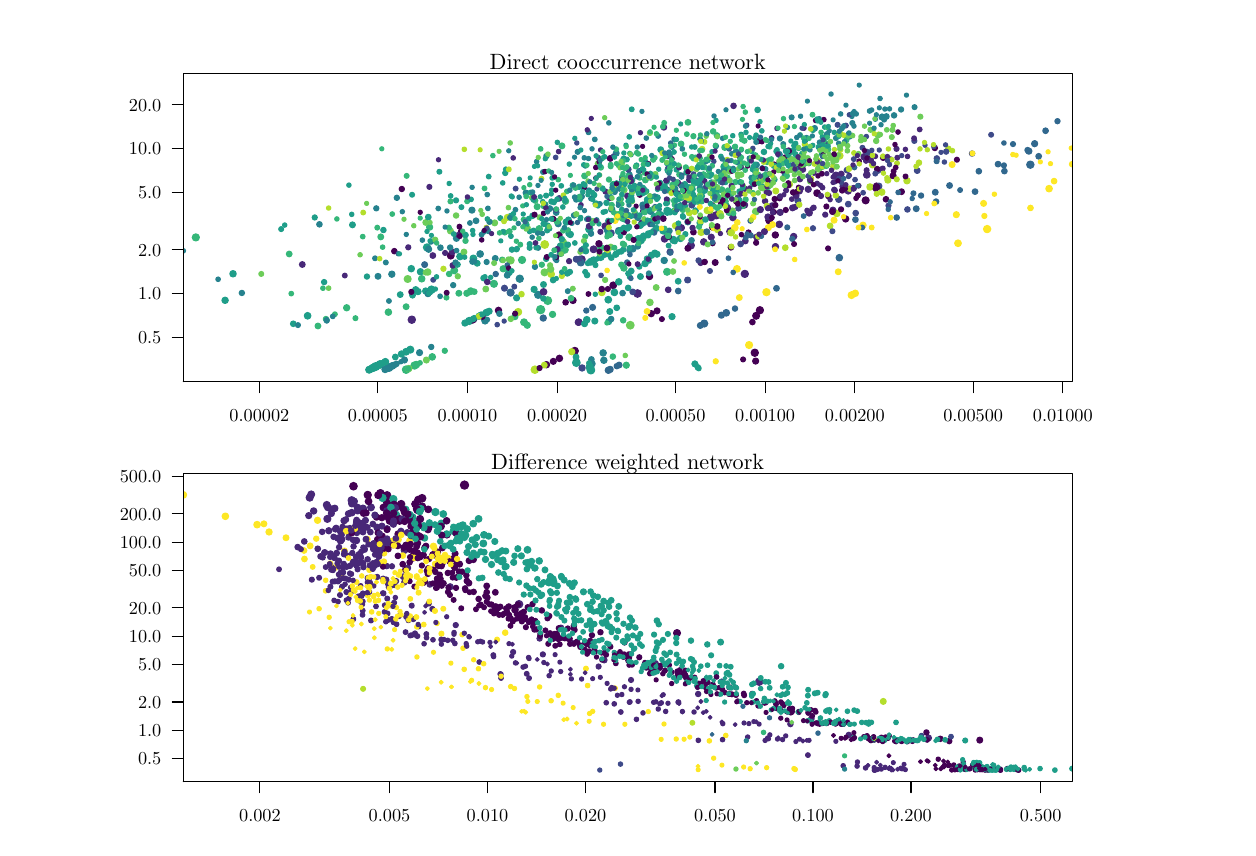
\begin{tikzpicture}[x=1pt,y=1pt]
\definecolor{fillColor}{RGB}{255,255,255}
\path[use as bounding box,fill=fillColor,fill opacity=0.00] (0,0) rectangle (433.62,289.08);
\begin{scope}
\path[clip] ( 56.23,161.17) rectangle (377.39,272.45);
\definecolor{drawColor}{RGB}{53,183,121}
\definecolor{fillColor}{RGB}{53,183,121}

\path[draw=drawColor,line width= 0.4pt,line join=round,line cap=round,fill=fillColor] (185.36,187.18) circle (  1.49);
\definecolor{drawColor}{RGB}{31,158,137}
\definecolor{fillColor}{RGB}{31,158,137}

\path[draw=drawColor,line width= 0.4pt,line join=round,line cap=round,fill=fillColor] (125.75,166.63) circle (  1.43);
\definecolor{drawColor}{RGB}{53,183,121}
\definecolor{fillColor}{RGB}{53,183,121}

\path[draw=drawColor,line width= 0.4pt,line join=round,line cap=round,fill=fillColor] (187.93,190.45) circle (  1.41);
\definecolor{drawColor}{RGB}{38,130,142}
\definecolor{fillColor}{RGB}{38,130,142}

\path[draw=drawColor,line width= 0.4pt,line join=round,line cap=round,fill=fillColor] (130.52,166.25) circle (  1.41);
\definecolor{drawColor}{RGB}{109,205,89}
\definecolor{fillColor}{RGB}{109,205,89}

\path[draw=drawColor,line width= 0.4pt,line join=round,line cap=round,fill=fillColor] (217.74,181.57) circle (  1.39);
\definecolor{drawColor}{RGB}{31,158,137}
\definecolor{fillColor}{RGB}{31,158,137}

\path[draw=drawColor,line width= 0.4pt,line join=round,line cap=round,fill=fillColor] (203.51,165.33) circle (  1.39);

\path[draw=drawColor,line width= 0.4pt,line join=round,line cap=round,fill=fillColor] (127.33,167.39) circle (  1.39);

\path[draw=drawColor,line width= 0.4pt,line join=round,line cap=round,fill=fillColor] (198.27,168.03) circle (  1.39);
\definecolor{drawColor}{RGB}{180,222,44}
\definecolor{fillColor}{RGB}{180,222,44}

\path[draw=drawColor,line width= 0.4pt,line join=round,line cap=round,fill=fillColor] (186.84,210.73) circle (  1.39);
\definecolor{drawColor}{RGB}{72,40,120}
\definecolor{fillColor}{RGB}{72,40,120}

\path[draw=drawColor,line width= 0.4pt,line join=round,line cap=round,fill=fillColor] (220.35,193.02) circle (  1.36);
\definecolor{drawColor}{RGB}{31,158,137}
\definecolor{fillColor}{RGB}{31,158,137}

\path[draw=drawColor,line width= 0.4pt,line join=round,line cap=round,fill=fillColor] (203.24,166.25) circle (  1.36);
\definecolor{drawColor}{RGB}{53,183,121}
\definecolor{fillColor}{RGB}{53,183,121}

\path[draw=drawColor,line width= 0.4pt,line join=round,line cap=round,fill=fillColor] (136.74,165.50) circle (  1.35);
\definecolor{drawColor}{RGB}{180,222,44}
\definecolor{fillColor}{RGB}{180,222,44}

\path[draw=drawColor,line width= 0.4pt,line join=round,line cap=round,fill=fillColor] (183.27,165.48) circle (  1.35);
\definecolor{drawColor}{RGB}{31,158,137}
\definecolor{fillColor}{RGB}{31,158,137}

\path[draw=drawColor,line width= 0.4pt,line join=round,line cap=round,fill=fillColor] (145.91,194.39) circle (  1.34);
\definecolor{drawColor}{RGB}{72,40,120}
\definecolor{fillColor}{RGB}{72,40,120}

\path[draw=drawColor,line width= 0.4pt,line join=round,line cap=round,fill=fillColor] (246.98,220.60) circle (  1.34);

\path[draw=drawColor,line width= 0.4pt,line join=round,line cap=round,fill=fillColor] (138.80,183.55) circle (  1.33);
\definecolor{drawColor}{RGB}{253,231,37}
\definecolor{fillColor}{RGB}{253,231,37}

\path[draw=drawColor,line width= 0.4pt,line join=round,line cap=round,fill=fillColor] (346.70,216.30) circle (  1.32);
\definecolor{drawColor}{RGB}{31,158,137}
\definecolor{fillColor}{RGB}{31,158,137}

\path[draw=drawColor,line width= 0.4pt,line join=round,line cap=round,fill=fillColor] (202.96,216.26) circle (  1.32);
\definecolor{drawColor}{RGB}{49,104,142}
\definecolor{fillColor}{RGB}{49,104,142}

\path[draw=drawColor,line width= 0.4pt,line join=round,line cap=round,fill=fillColor] (362.31,239.57) circle (  1.32);
\definecolor{drawColor}{RGB}{72,40,120}
\definecolor{fillColor}{RGB}{72,40,120}

\path[draw=drawColor,line width= 0.4pt,line join=round,line cap=round,fill=fillColor] (248.83,221.27) circle (  1.32);

\path[draw=drawColor,line width= 0.4pt,line join=round,line cap=round,fill=fillColor] (292.06,235.61) circle (  1.31);
\definecolor{drawColor}{RGB}{38,130,142}
\definecolor{fillColor}{RGB}{38,130,142}

\path[draw=drawColor,line width= 0.4pt,line join=round,line cap=round,fill=fillColor] (177.81,198.37) circle (  1.31);
\definecolor{drawColor}{RGB}{68,1,84}
\definecolor{fillColor}{RGB}{68,1,84}

\path[draw=drawColor,line width= 0.4pt,line join=round,line cap=round,fill=fillColor] (262.74,171.61) circle (  1.31);
\definecolor{drawColor}{RGB}{31,158,137}
\definecolor{fillColor}{RGB}{31,158,137}

\path[draw=drawColor,line width= 0.4pt,line join=round,line cap=round,fill=fillColor] (124.94,166.23) circle (  1.31);
\definecolor{drawColor}{RGB}{72,40,120}
\definecolor{fillColor}{RGB}{72,40,120}

\path[draw=drawColor,line width= 0.4pt,line join=round,line cap=round,fill=fillColor] (200.16,205.33) circle (  1.31);
\definecolor{drawColor}{RGB}{53,183,121}
\definecolor{fillColor}{RGB}{53,183,121}

\path[draw=drawColor,line width= 0.4pt,line join=round,line cap=round,fill=fillColor] (139.79,166.99) circle (  1.31);
\definecolor{drawColor}{RGB}{31,158,137}
\definecolor{fillColor}{RGB}{31,158,137}

\path[draw=drawColor,line width= 0.4pt,line join=round,line cap=round,fill=fillColor] (144.30,209.66) circle (  1.30);
\definecolor{drawColor}{RGB}{253,231,37}
\definecolor{fillColor}{RGB}{253,231,37}

\path[draw=drawColor,line width= 0.4pt,line join=round,line cap=round,fill=fillColor] (266.94,193.50) circle (  1.30);
\definecolor{drawColor}{RGB}{31,158,137}
\definecolor{fillColor}{RGB}{31,158,137}

\path[draw=drawColor,line width= 0.4pt,line join=round,line cap=round,fill=fillColor] (215.92,220.04) circle (  1.30);
\definecolor{drawColor}{RGB}{72,40,120}
\definecolor{fillColor}{RGB}{72,40,120}

\path[draw=drawColor,line width= 0.4pt,line join=round,line cap=round,fill=fillColor] (259.14,200.11) circle (  1.30);
\definecolor{drawColor}{RGB}{31,158,137}
\definecolor{fillColor}{RGB}{31,158,137}

\path[draw=drawColor,line width= 0.4pt,line join=round,line cap=round,fill=fillColor] (207.04,206.23) circle (  1.30);
\definecolor{drawColor}{RGB}{109,205,89}
\definecolor{fillColor}{RGB}{109,205,89}

\path[draw=drawColor,line width= 0.4pt,line join=round,line cap=round,fill=fillColor] (174.50,205.00) circle (  1.30);
\definecolor{drawColor}{RGB}{53,183,121}
\definecolor{fillColor}{RGB}{53,183,121}

\path[draw=drawColor,line width= 0.4pt,line join=round,line cap=round,fill=fillColor] (222.13,213.09) circle (  1.30);
\definecolor{drawColor}{RGB}{72,40,120}
\definecolor{fillColor}{RGB}{72,40,120}

\path[draw=drawColor,line width= 0.4pt,line join=round,line cap=round,fill=fillColor] (253.88,215.42) circle (  1.30);
\definecolor{drawColor}{RGB}{31,158,137}
\definecolor{fillColor}{RGB}{31,158,137}

\path[draw=drawColor,line width= 0.4pt,line join=round,line cap=round,fill=fillColor] (231.15,222.89) circle (  1.30);

\path[draw=drawColor,line width= 0.4pt,line join=round,line cap=round,fill=fillColor] (159.57,183.10) circle (  1.30);
\definecolor{drawColor}{RGB}{68,1,84}
\definecolor{fillColor}{RGB}{68,1,84}

\path[draw=drawColor,line width= 0.4pt,line join=round,line cap=round,fill=fillColor] (197.70,172.28) circle (  1.29);

\path[draw=drawColor,line width= 0.4pt,line join=round,line cap=round,fill=fillColor] (264.59,186.98) circle (  1.29);
\definecolor{drawColor}{RGB}{49,104,142}
\definecolor{fillColor}{RGB}{49,104,142}

\path[draw=drawColor,line width= 0.4pt,line join=round,line cap=round,fill=fillColor] (174.51,193.35) circle (  1.29);
\definecolor{drawColor}{RGB}{53,183,121}
\definecolor{fillColor}{RGB}{53,183,121}

\path[draw=drawColor,line width= 0.4pt,line join=round,line cap=round,fill=fillColor] (251.75,238.81) circle (  1.29);

\path[draw=drawColor,line width= 0.4pt,line join=round,line cap=round,fill=fillColor] ( 60.76,213.29) circle (  1.29);
\definecolor{drawColor}{RGB}{31,158,137}
\definecolor{fillColor}{RGB}{31,158,137}

\path[draw=drawColor,line width= 0.4pt,line join=round,line cap=round,fill=fillColor] (233.35,212.38) circle (  1.28);
\definecolor{drawColor}{RGB}{38,130,142}
\definecolor{fillColor}{RGB}{38,130,142}

\path[draw=drawColor,line width= 0.4pt,line join=round,line cap=round,fill=fillColor] (184.45,192.53) circle (  1.28);
\definecolor{drawColor}{RGB}{72,40,120}
\definecolor{fillColor}{RGB}{72,40,120}

\path[draw=drawColor,line width= 0.4pt,line join=round,line cap=round,fill=fillColor] (239.64,210.38) circle (  1.28);
\definecolor{drawColor}{RGB}{53,183,121}
\definecolor{fillColor}{RGB}{53,183,121}

\path[draw=drawColor,line width= 0.4pt,line join=round,line cap=round,fill=fillColor] (178.64,205.14) circle (  1.28);
\definecolor{drawColor}{RGB}{31,158,137}
\definecolor{fillColor}{RGB}{31,158,137}

\path[draw=drawColor,line width= 0.4pt,line join=round,line cap=round,fill=fillColor] (231.54,237.64) circle (  1.28);
\definecolor{drawColor}{RGB}{109,205,89}
\definecolor{fillColor}{RGB}{109,205,89}

\path[draw=drawColor,line width= 0.4pt,line join=round,line cap=round,fill=fillColor] (285.72,240.53) circle (  1.28);
\definecolor{drawColor}{RGB}{49,104,142}
\definecolor{fillColor}{RGB}{49,104,142}

\path[draw=drawColor,line width= 0.4pt,line join=round,line cap=round,fill=fillColor] (199.87,204.24) circle (  1.27);

\path[draw=drawColor,line width= 0.4pt,line join=round,line cap=round,fill=fillColor] (244.48,182.17) circle (  1.27);
\definecolor{drawColor}{RGB}{31,158,137}
\definecolor{fillColor}{RGB}{31,158,137}

\path[draw=drawColor,line width= 0.4pt,line join=round,line cap=round,fill=fillColor] (204.52,205.00) circle (  1.27);
\definecolor{drawColor}{RGB}{180,222,44}
\definecolor{fillColor}{RGB}{180,222,44}

\path[draw=drawColor,line width= 0.4pt,line join=round,line cap=round,fill=fillColor] (177.24,186.34) circle (  1.27);
\definecolor{drawColor}{RGB}{31,158,137}
\definecolor{fillColor}{RGB}{31,158,137}

\path[draw=drawColor,line width= 0.4pt,line join=round,line cap=round,fill=fillColor] (203.19,166.44) circle (  1.27);
\definecolor{drawColor}{RGB}{253,231,37}
\definecolor{fillColor}{RGB}{253,231,37}

\path[draw=drawColor,line width= 0.4pt,line join=round,line cap=round,fill=fillColor] (260.68,174.40) circle (  1.27);
\definecolor{drawColor}{RGB}{68,1,84}
\definecolor{fillColor}{RGB}{68,1,84}

\path[draw=drawColor,line width= 0.4pt,line join=round,line cap=round,fill=fillColor] (302.80,226.68) circle (  1.27);
\definecolor{drawColor}{RGB}{31,158,137}
\definecolor{fillColor}{RGB}{31,158,137}

\path[draw=drawColor,line width= 0.4pt,line join=round,line cap=round,fill=fillColor] (124.46,165.99) circle (  1.26);
\definecolor{drawColor}{RGB}{180,222,44}
\definecolor{fillColor}{RGB}{180,222,44}

\path[draw=drawColor,line width= 0.4pt,line join=round,line cap=round,fill=fillColor] (293.37,242.80) circle (  1.26);
\definecolor{drawColor}{RGB}{31,158,137}
\definecolor{fillColor}{RGB}{31,158,137}

\path[draw=drawColor,line width= 0.4pt,line join=round,line cap=round,fill=fillColor] (138.27,172.73) circle (  1.26);

\path[draw=drawColor,line width= 0.4pt,line join=round,line cap=round,fill=fillColor] (174.48,220.67) circle (  1.26);
\definecolor{drawColor}{RGB}{53,183,121}
\definecolor{fillColor}{RGB}{53,183,121}

\path[draw=drawColor,line width= 0.4pt,line join=round,line cap=round,fill=fillColor] (168.49,196.52) circle (  1.26);
\definecolor{drawColor}{RGB}{109,205,89}
\definecolor{fillColor}{RGB}{109,205,89}

\path[draw=drawColor,line width= 0.4pt,line join=round,line cap=round,fill=fillColor] (137.31,198.26) circle (  1.25);
\definecolor{drawColor}{RGB}{53,183,121}
\definecolor{fillColor}{RGB}{53,183,121}

\path[draw=drawColor,line width= 0.4pt,line join=round,line cap=round,fill=fillColor] (231.03,200.86) circle (  1.25);
\definecolor{drawColor}{RGB}{109,205,89}
\definecolor{fillColor}{RGB}{109,205,89}

\path[draw=drawColor,line width= 0.4pt,line join=round,line cap=round,fill=fillColor] (186.77,200.65) circle (  1.25);
\definecolor{drawColor}{RGB}{68,1,84}
\definecolor{fillColor}{RGB}{68,1,84}

\path[draw=drawColor,line width= 0.4pt,line join=round,line cap=round,fill=fillColor] (263.23,184.97) circle (  1.25);

\path[draw=drawColor,line width= 0.4pt,line join=round,line cap=round,fill=fillColor] (152.87,206.71) circle (  1.24);
\definecolor{drawColor}{RGB}{31,158,137}
\definecolor{fillColor}{RGB}{31,158,137}

\path[draw=drawColor,line width= 0.4pt,line join=round,line cap=round,fill=fillColor] (226.51,220.72) circle (  1.24);
\definecolor{drawColor}{RGB}{72,40,120}
\definecolor{fillColor}{RGB}{72,40,120}

\path[draw=drawColor,line width= 0.4pt,line join=round,line cap=round,fill=fillColor] (204.49,208.99) circle (  1.23);
\definecolor{drawColor}{RGB}{253,231,37}
\definecolor{fillColor}{RGB}{253,231,37}

\path[draw=drawColor,line width= 0.4pt,line join=round,line cap=round,fill=fillColor] (297.69,192.43) circle (  1.23);
\definecolor{drawColor}{RGB}{72,40,120}
\definecolor{fillColor}{RGB}{72,40,120}

\path[draw=drawColor,line width= 0.4pt,line join=round,line cap=round,fill=fillColor] (208.76,217.32) circle (  1.23);
\definecolor{drawColor}{RGB}{53,183,121}
\definecolor{fillColor}{RGB}{53,183,121}

\path[draw=drawColor,line width= 0.4pt,line join=round,line cap=round,fill=fillColor] (238.32,231.01) circle (  1.23);
\definecolor{drawColor}{RGB}{68,1,84}
\definecolor{fillColor}{RGB}{68,1,84}

\path[draw=drawColor,line width= 0.4pt,line join=round,line cap=round,fill=fillColor] (267.92,219.44) circle (  1.22);
\definecolor{drawColor}{RGB}{53,183,121}
\definecolor{fillColor}{RGB}{53,183,121}

\path[draw=drawColor,line width= 0.4pt,line join=round,line cap=round,fill=fillColor] (154.15,201.36) circle (  1.22);
\definecolor{drawColor}{RGB}{109,205,89}
\definecolor{fillColor}{RGB}{109,205,89}

\path[draw=drawColor,line width= 0.4pt,line join=round,line cap=round,fill=fillColor] (263.12,222.62) circle (  1.22);
\definecolor{drawColor}{RGB}{31,158,137}
\definecolor{fillColor}{RGB}{31,158,137}

\path[draw=drawColor,line width= 0.4pt,line join=round,line cap=round,fill=fillColor] (123.38,165.47) circle (  1.22);
\definecolor{drawColor}{RGB}{53,183,121}
\definecolor{fillColor}{RGB}{53,183,121}

\path[draw=drawColor,line width= 0.4pt,line join=round,line cap=round,fill=fillColor] (160.09,193.87) circle (  1.22);
\definecolor{drawColor}{RGB}{31,158,137}
\definecolor{fillColor}{RGB}{31,158,137}

\path[draw=drawColor,line width= 0.4pt,line join=round,line cap=round,fill=fillColor] (161.06,205.69) circle (  1.22);
\definecolor{drawColor}{RGB}{38,130,142}
\definecolor{fillColor}{RGB}{38,130,142}

\path[draw=drawColor,line width= 0.4pt,line join=round,line cap=round,fill=fillColor] (203.84,167.65) circle (  1.22);
\definecolor{drawColor}{RGB}{53,183,121}
\definecolor{fillColor}{RGB}{53,183,121}

\path[draw=drawColor,line width= 0.4pt,line join=round,line cap=round,fill=fillColor] (179.35,182.64) circle (  1.22);
\definecolor{drawColor}{RGB}{38,130,142}
\definecolor{fillColor}{RGB}{38,130,142}

\path[draw=drawColor,line width= 0.4pt,line join=round,line cap=round,fill=fillColor] (131.77,166.86) circle (  1.22);
\definecolor{drawColor}{RGB}{180,222,44}
\definecolor{fillColor}{RGB}{180,222,44}

\path[draw=drawColor,line width= 0.4pt,line join=round,line cap=round,fill=fillColor] (280.16,239.79) circle (  1.22);
\definecolor{drawColor}{RGB}{38,130,142}
\definecolor{fillColor}{RGB}{38,130,142}

\path[draw=drawColor,line width= 0.4pt,line join=round,line cap=round,fill=fillColor] (192.58,207.62) circle (  1.22);
\definecolor{drawColor}{RGB}{31,158,137}
\definecolor{fillColor}{RGB}{31,158,137}

\path[draw=drawColor,line width= 0.4pt,line join=round,line cap=round,fill=fillColor] (203.49,165.39) circle (  1.21);
\definecolor{drawColor}{RGB}{38,130,142}
\definecolor{fillColor}{RGB}{38,130,142}

\path[draw=drawColor,line width= 0.4pt,line join=round,line cap=round,fill=fillColor] (266.10,235.24) circle (  1.21);
\definecolor{drawColor}{RGB}{68,1,84}
\definecolor{fillColor}{RGB}{68,1,84}

\path[draw=drawColor,line width= 0.4pt,line join=round,line cap=round,fill=fillColor] (211.58,195.98) circle (  1.21);
\definecolor{drawColor}{RGB}{31,158,137}
\definecolor{fillColor}{RGB}{31,158,137}

\path[draw=drawColor,line width= 0.4pt,line join=round,line cap=round,fill=fillColor] (173.95,200.71) circle (  1.21);
\definecolor{drawColor}{RGB}{53,183,121}
\definecolor{fillColor}{RGB}{53,183,121}

\path[draw=drawColor,line width= 0.4pt,line join=round,line cap=round,fill=fillColor] (252.22,224.91) circle (  1.21);
\definecolor{drawColor}{RGB}{31,158,137}
\definecolor{fillColor}{RGB}{31,158,137}

\path[draw=drawColor,line width= 0.4pt,line join=round,line cap=round,fill=fillColor] (136.72,171.97) circle (  1.21);
\definecolor{drawColor}{RGB}{253,231,37}
\definecolor{fillColor}{RGB}{253,231,37}

\path[draw=drawColor,line width= 0.4pt,line join=round,line cap=round,fill=fillColor] (256.30,201.93) circle (  1.21);
\definecolor{drawColor}{RGB}{38,130,142}
\definecolor{fillColor}{RGB}{38,130,142}

\path[draw=drawColor,line width= 0.4pt,line join=round,line cap=round,fill=fillColor] (273.83,235.69) circle (  1.21);
\definecolor{drawColor}{RGB}{31,158,137}
\definecolor{fillColor}{RGB}{31,158,137}

\path[draw=drawColor,line width= 0.4pt,line join=round,line cap=round,fill=fillColor] (165.83,186.15) circle (  1.20);

\path[draw=drawColor,line width= 0.4pt,line join=round,line cap=round,fill=fillColor] (212.01,193.42) circle (  1.20);
\definecolor{drawColor}{RGB}{38,130,142}
\definecolor{fillColor}{RGB}{38,130,142}

\path[draw=drawColor,line width= 0.4pt,line join=round,line cap=round,fill=fillColor] (165.28,183.19) circle (  1.20);
\definecolor{drawColor}{RGB}{49,104,142}
\definecolor{fillColor}{RGB}{49,104,142}

\path[draw=drawColor,line width= 0.4pt,line join=round,line cap=round,fill=fillColor] (252.42,186.03) circle (  1.20);
\definecolor{drawColor}{RGB}{31,158,137}
\definecolor{fillColor}{RGB}{31,158,137}

\path[draw=drawColor,line width= 0.4pt,line join=round,line cap=round,fill=fillColor] (156.23,206.39) circle (  1.20);
\definecolor{drawColor}{RGB}{53,183,121}
\definecolor{fillColor}{RGB}{53,183,121}

\path[draw=drawColor,line width= 0.4pt,line join=round,line cap=round,fill=fillColor] (248.77,231.28) circle (  1.20);
\definecolor{drawColor}{RGB}{31,158,137}
\definecolor{fillColor}{RGB}{31,158,137}

\path[draw=drawColor,line width= 0.4pt,line join=round,line cap=round,fill=fillColor] (203.12,166.68) circle (  1.20);

\path[draw=drawColor,line width= 0.4pt,line join=round,line cap=round,fill=fillColor] (209.80,190.78) circle (  1.20);
\definecolor{drawColor}{RGB}{253,231,37}
\definecolor{fillColor}{RGB}{253,231,37}

\path[draw=drawColor,line width= 0.4pt,line join=round,line cap=round,fill=fillColor] (255.53,216.79) circle (  1.20);

\path[draw=drawColor,line width= 0.4pt,line join=round,line cap=round,fill=fillColor] (336.17,211.18) circle (  1.20);
\definecolor{drawColor}{RGB}{72,40,120}
\definecolor{fillColor}{RGB}{72,40,120}

\path[draw=drawColor,line width= 0.4pt,line join=round,line cap=round,fill=fillColor] (302.31,242.41) circle (  1.20);
\definecolor{drawColor}{RGB}{68,1,84}
\definecolor{fillColor}{RGB}{68,1,84}

\path[draw=drawColor,line width= 0.4pt,line join=round,line cap=round,fill=fillColor] (285.25,229.30) circle (  1.20);
\definecolor{drawColor}{RGB}{31,158,137}
\definecolor{fillColor}{RGB}{31,158,137}

\path[draw=drawColor,line width= 0.4pt,line join=round,line cap=round,fill=fillColor] (203.42,204.46) circle (  1.19);

\path[draw=drawColor,line width= 0.4pt,line join=round,line cap=round,fill=fillColor] (145.19,193.67) circle (  1.19);
\definecolor{drawColor}{RGB}{109,205,89}
\definecolor{fillColor}{RGB}{109,205,89}

\path[draw=drawColor,line width= 0.4pt,line join=round,line cap=round,fill=fillColor] (285.80,238.04) circle (  1.19);
\definecolor{drawColor}{RGB}{72,40,120}
\definecolor{fillColor}{RGB}{72,40,120}

\path[draw=drawColor,line width= 0.4pt,line join=round,line cap=round,fill=fillColor] (303.21,235.89) circle (  1.19);
\definecolor{drawColor}{RGB}{180,222,44}
\definecolor{fillColor}{RGB}{180,222,44}

\path[draw=drawColor,line width= 0.4pt,line join=round,line cap=round,fill=fillColor] (292.35,221.95) circle (  1.19);
\definecolor{drawColor}{RGB}{53,183,121}
\definecolor{fillColor}{RGB}{53,183,121}

\path[draw=drawColor,line width= 0.4pt,line join=round,line cap=round,fill=fillColor] (140.46,167.32) circle (  1.19);
\definecolor{drawColor}{RGB}{72,40,120}
\definecolor{fillColor}{RGB}{72,40,120}

\path[draw=drawColor,line width= 0.4pt,line join=round,line cap=round,fill=fillColor] (186.41,193.61) circle (  1.19);
\definecolor{drawColor}{RGB}{53,183,121}
\definecolor{fillColor}{RGB}{53,183,121}

\path[draw=drawColor,line width= 0.4pt,line join=round,line cap=round,fill=fillColor] (207.13,209.49) circle (  1.19);
\definecolor{drawColor}{RGB}{38,130,142}
\definecolor{fillColor}{RGB}{38,130,142}

\path[draw=drawColor,line width= 0.4pt,line join=round,line cap=round,fill=fillColor] (218.68,209.20) circle (  1.19);
\definecolor{drawColor}{RGB}{31,158,137}
\definecolor{fillColor}{RGB}{31,158,137}

\path[draw=drawColor,line width= 0.4pt,line join=round,line cap=round,fill=fillColor] (101.15,184.97) circle (  1.19);
\definecolor{drawColor}{RGB}{180,222,44}
\definecolor{fillColor}{RGB}{180,222,44}

\path[draw=drawColor,line width= 0.4pt,line join=round,line cap=round,fill=fillColor] (250.17,221.83) circle (  1.19);
\definecolor{drawColor}{RGB}{31,158,137}
\definecolor{fillColor}{RGB}{31,158,137}

\path[draw=drawColor,line width= 0.4pt,line join=round,line cap=round,fill=fillColor] (129.26,168.34) circle (  1.19);
\definecolor{drawColor}{RGB}{53,183,121}
\definecolor{fillColor}{RGB}{53,183,121}

\path[draw=drawColor,line width= 0.4pt,line join=round,line cap=round,fill=fillColor] (184.86,216.36) circle (  1.19);
\definecolor{drawColor}{RGB}{72,40,120}
\definecolor{fillColor}{RGB}{72,40,120}

\path[draw=drawColor,line width= 0.4pt,line join=round,line cap=round,fill=fillColor] (278.79,230.13) circle (  1.19);

\path[draw=drawColor,line width= 0.4pt,line join=round,line cap=round,fill=fillColor] (221.98,218.39) circle (  1.19);
\definecolor{drawColor}{RGB}{180,222,44}
\definecolor{fillColor}{RGB}{180,222,44}

\path[draw=drawColor,line width= 0.4pt,line join=round,line cap=round,fill=fillColor] (245.60,223.03) circle (  1.18);
\definecolor{drawColor}{RGB}{72,40,120}
\definecolor{fillColor}{RGB}{72,40,120}

\path[draw=drawColor,line width= 0.4pt,line join=round,line cap=round,fill=fillColor] (271.59,217.99) circle (  1.18);
\definecolor{drawColor}{RGB}{53,183,121}
\definecolor{fillColor}{RGB}{53,183,121}

\path[draw=drawColor,line width= 0.4pt,line join=round,line cap=round,fill=fillColor] (146.19,170.11) circle (  1.18);
\definecolor{drawColor}{RGB}{72,40,120}
\definecolor{fillColor}{RGB}{72,40,120}

\path[draw=drawColor,line width= 0.4pt,line join=round,line cap=round,fill=fillColor] (222.64,222.80) circle (  1.18);
\definecolor{drawColor}{RGB}{253,231,37}
\definecolor{fillColor}{RGB}{253,231,37}

\path[draw=drawColor,line width= 0.4pt,line join=round,line cap=round,fill=fillColor] (369.08,230.91) circle (  1.18);
\definecolor{drawColor}{RGB}{38,130,142}
\definecolor{fillColor}{RGB}{38,130,142}

\path[draw=drawColor,line width= 0.4pt,line join=round,line cap=round,fill=fillColor] (163.50,207.30) circle (  1.18);
\definecolor{drawColor}{RGB}{53,183,121}
\definecolor{fillColor}{RGB}{53,183,121}

\path[draw=drawColor,line width= 0.4pt,line join=round,line cap=round,fill=fillColor] (217.37,213.35) circle (  1.18);
\definecolor{drawColor}{RGB}{180,222,44}
\definecolor{fillColor}{RGB}{180,222,44}

\path[draw=drawColor,line width= 0.4pt,line join=round,line cap=round,fill=fillColor] (189.18,199.98) circle (  1.18);
\definecolor{drawColor}{RGB}{72,40,120}
\definecolor{fillColor}{RGB}{72,40,120}

\path[draw=drawColor,line width= 0.4pt,line join=round,line cap=round,fill=fillColor] (199.15,182.69) circle (  1.17);

\path[draw=drawColor,line width= 0.4pt,line join=round,line cap=round,fill=fillColor] (296.49,230.12) circle (  1.17);
\definecolor{drawColor}{RGB}{180,222,44}
\definecolor{fillColor}{RGB}{180,222,44}

\path[draw=drawColor,line width= 0.4pt,line join=round,line cap=round,fill=fillColor] (254.19,214.98) circle (  1.17);
\definecolor{drawColor}{RGB}{38,130,142}
\definecolor{fillColor}{RGB}{38,130,142}

\path[draw=drawColor,line width= 0.4pt,line join=round,line cap=round,fill=fillColor] (262.93,237.77) circle (  1.17);
\definecolor{drawColor}{RGB}{31,158,137}
\definecolor{fillColor}{RGB}{31,158,137}

\path[draw=drawColor,line width= 0.4pt,line join=round,line cap=round,fill=fillColor] (202.03,183.55) circle (  1.17);
\definecolor{drawColor}{RGB}{49,104,142}
\definecolor{fillColor}{RGB}{49,104,142}

\path[draw=drawColor,line width= 0.4pt,line join=round,line cap=round,fill=fillColor] (293.29,205.95) circle (  1.17);
\definecolor{drawColor}{RGB}{72,40,120}
\definecolor{fillColor}{RGB}{72,40,120}

\path[draw=drawColor,line width= 0.4pt,line join=round,line cap=round,fill=fillColor] (230.13,212.74) circle (  1.17);

\path[draw=drawColor,line width= 0.4pt,line join=round,line cap=round,fill=fillColor] (254.84,220.47) circle (  1.16);
\definecolor{drawColor}{RGB}{180,222,44}
\definecolor{fillColor}{RGB}{180,222,44}

\path[draw=drawColor,line width= 0.4pt,line join=round,line cap=round,fill=fillColor] (243.38,215.14) circle (  1.16);

\path[draw=drawColor,line width= 0.4pt,line join=round,line cap=round,fill=fillColor] (304.38,231.51) circle (  1.16);
\definecolor{drawColor}{RGB}{31,158,137}
\definecolor{fillColor}{RGB}{31,158,137}

\path[draw=drawColor,line width= 0.4pt,line join=round,line cap=round,fill=fillColor] (163.77,185.15) circle (  1.16);

\path[draw=drawColor,line width= 0.4pt,line join=round,line cap=round,fill=fillColor] ( 74.20,200.15) circle (  1.16);
\definecolor{drawColor}{RGB}{53,183,121}
\definecolor{fillColor}{RGB}{53,183,121}

\path[draw=drawColor,line width= 0.4pt,line join=round,line cap=round,fill=fillColor] (142.39,198.34) circle (  1.16);
\definecolor{drawColor}{RGB}{180,222,44}
\definecolor{fillColor}{RGB}{180,222,44}

\path[draw=drawColor,line width= 0.4pt,line join=round,line cap=round,fill=fillColor] (275.22,232.47) circle (  1.16);

\path[draw=drawColor,line width= 0.4pt,line join=round,line cap=round,fill=fillColor] (279.49,239.51) circle (  1.16);
\definecolor{drawColor}{RGB}{72,40,120}
\definecolor{fillColor}{RGB}{72,40,120}

\path[draw=drawColor,line width= 0.4pt,line join=round,line cap=round,fill=fillColor] (282.39,222.15) circle (  1.16);
\definecolor{drawColor}{RGB}{109,205,89}
\definecolor{fillColor}{RGB}{109,205,89}

\path[draw=drawColor,line width= 0.4pt,line join=round,line cap=round,fill=fillColor] (224.85,189.80) circle (  1.16);
\definecolor{drawColor}{RGB}{31,158,137}
\definecolor{fillColor}{RGB}{31,158,137}

\path[draw=drawColor,line width= 0.4pt,line join=round,line cap=round,fill=fillColor] (235.88,212.91) circle (  1.16);
\definecolor{drawColor}{RGB}{53,183,121}
\definecolor{fillColor}{RGB}{53,183,121}

\path[draw=drawColor,line width= 0.4pt,line join=round,line cap=round,fill=fillColor] (130.35,186.28) circle (  1.16);
\definecolor{drawColor}{RGB}{253,231,37}
\definecolor{fillColor}{RGB}{253,231,37}

\path[draw=drawColor,line width= 0.4pt,line join=round,line cap=round,fill=fillColor] (299.04,193.09) circle (  1.16);
\definecolor{drawColor}{RGB}{109,205,89}
\definecolor{fillColor}{RGB}{109,205,89}

\path[draw=drawColor,line width= 0.4pt,line join=round,line cap=round,fill=fillColor] (144.57,200.78) circle (  1.16);
\definecolor{drawColor}{RGB}{68,1,84}
\definecolor{fillColor}{RGB}{68,1,84}

\path[draw=drawColor,line width= 0.4pt,line join=round,line cap=round,fill=fillColor] (197.03,190.54) circle (  1.16);
\definecolor{drawColor}{RGB}{180,222,44}
\definecolor{fillColor}{RGB}{180,222,44}

\path[draw=drawColor,line width= 0.4pt,line join=round,line cap=round,fill=fillColor] (207.48,193.38) circle (  1.16);

\path[draw=drawColor,line width= 0.4pt,line join=round,line cap=round,fill=fillColor] (308.62,229.67) circle (  1.16);
\definecolor{drawColor}{RGB}{253,231,37}
\definecolor{fillColor}{RGB}{253,231,37}

\path[draw=drawColor,line width= 0.4pt,line join=round,line cap=round,fill=fillColor] (301.83,217.68) circle (  1.15);
\definecolor{drawColor}{RGB}{68,1,84}
\definecolor{fillColor}{RGB}{68,1,84}

\path[draw=drawColor,line width= 0.4pt,line join=round,line cap=round,fill=fillColor] (306.75,231.80) circle (  1.15);
\definecolor{drawColor}{RGB}{72,40,120}
\definecolor{fillColor}{RGB}{72,40,120}

\path[draw=drawColor,line width= 0.4pt,line join=round,line cap=round,fill=fillColor] (259.01,225.02) circle (  1.15);
\definecolor{drawColor}{RGB}{31,158,137}
\definecolor{fillColor}{RGB}{31,158,137}

\path[draw=drawColor,line width= 0.4pt,line join=round,line cap=round,fill=fillColor] (213.59,197.24) circle (  1.15);
\definecolor{drawColor}{RGB}{38,130,142}
\definecolor{fillColor}{RGB}{38,130,142}

\path[draw=drawColor,line width= 0.4pt,line join=round,line cap=round,fill=fillColor] (207.94,171.56) circle (  1.15);
\definecolor{drawColor}{RGB}{180,222,44}
\definecolor{fillColor}{RGB}{180,222,44}

\path[draw=drawColor,line width= 0.4pt,line join=round,line cap=round,fill=fillColor] (293.41,250.78) circle (  1.15);
\definecolor{drawColor}{RGB}{53,183,121}
\definecolor{fillColor}{RGB}{53,183,121}

\path[draw=drawColor,line width= 0.4pt,line join=round,line cap=round,fill=fillColor] (194.09,208.73) circle (  1.15);
\definecolor{drawColor}{RGB}{31,158,137}
\definecolor{fillColor}{RGB}{31,158,137}

\path[draw=drawColor,line width= 0.4pt,line join=round,line cap=round,fill=fillColor] (138.61,201.99) circle (  1.15);
\definecolor{drawColor}{RGB}{38,130,142}
\definecolor{fillColor}{RGB}{38,130,142}

\path[draw=drawColor,line width= 0.4pt,line join=round,line cap=round,fill=fillColor] (211.01,223.50) circle (  1.15);
\definecolor{drawColor}{RGB}{53,183,121}
\definecolor{fillColor}{RGB}{53,183,121}

\path[draw=drawColor,line width= 0.4pt,line join=round,line cap=round,fill=fillColor] (232.76,239.39) circle (  1.15);
\definecolor{drawColor}{RGB}{31,158,137}
\definecolor{fillColor}{RGB}{31,158,137}

\path[draw=drawColor,line width= 0.4pt,line join=round,line cap=round,fill=fillColor] (203.58,204.54) circle (  1.15);
\definecolor{drawColor}{RGB}{109,205,89}
\definecolor{fillColor}{RGB}{109,205,89}

\path[draw=drawColor,line width= 0.4pt,line join=round,line cap=round,fill=fillColor] (204.24,219.00) circle (  1.15);
\definecolor{drawColor}{RGB}{49,104,142}
\definecolor{fillColor}{RGB}{49,104,142}

\path[draw=drawColor,line width= 0.4pt,line join=round,line cap=round,fill=fillColor] (209.84,165.29) circle (  1.15);
\definecolor{drawColor}{RGB}{31,158,137}
\definecolor{fillColor}{RGB}{31,158,137}

\path[draw=drawColor,line width= 0.4pt,line join=round,line cap=round,fill=fillColor] (123.41,165.48) circle (  1.15);
\definecolor{drawColor}{RGB}{68,1,84}
\definecolor{fillColor}{RGB}{68,1,84}

\path[draw=drawColor,line width= 0.4pt,line join=round,line cap=round,fill=fillColor] (192.14,169.58) circle (  1.15);
\definecolor{drawColor}{RGB}{53,183,121}
\definecolor{fillColor}{RGB}{53,183,121}

\path[draw=drawColor,line width= 0.4pt,line join=round,line cap=round,fill=fillColor] (253.44,222.36) circle (  1.15);

\path[draw=drawColor,line width= 0.4pt,line join=round,line cap=round,fill=fillColor] (287.27,239.07) circle (  1.15);
\definecolor{drawColor}{RGB}{68,1,84}
\definecolor{fillColor}{RGB}{68,1,84}

\path[draw=drawColor,line width= 0.4pt,line join=round,line cap=round,fill=fillColor] (170.13,186.91) circle (  1.15);
\definecolor{drawColor}{RGB}{31,158,137}
\definecolor{fillColor}{RGB}{31,158,137}

\path[draw=drawColor,line width= 0.4pt,line join=round,line cap=round,fill=fillColor] (223.09,203.84) circle (  1.14);
\definecolor{drawColor}{RGB}{38,130,142}
\definecolor{fillColor}{RGB}{38,130,142}

\path[draw=drawColor,line width= 0.4pt,line join=round,line cap=round,fill=fillColor] (230.01,204.96) circle (  1.14);
\definecolor{drawColor}{RGB}{31,158,137}
\definecolor{fillColor}{RGB}{31,158,137}

\path[draw=drawColor,line width= 0.4pt,line join=round,line cap=round,fill=fillColor] (194.62,218.84) circle (  1.14);

\path[draw=drawColor,line width= 0.4pt,line join=round,line cap=round,fill=fillColor] ( 71.34,190.56) circle (  1.14);
\definecolor{drawColor}{RGB}{53,183,121}
\definecolor{fillColor}{RGB}{53,183,121}

\path[draw=drawColor,line width= 0.4pt,line join=round,line cap=round,fill=fillColor] (230.43,215.43) circle (  1.14);
\definecolor{drawColor}{RGB}{31,158,137}
\definecolor{fillColor}{RGB}{31,158,137}

\path[draw=drawColor,line width= 0.4pt,line join=round,line cap=round,fill=fillColor] (141.93,200.88) circle (  1.14);
\definecolor{drawColor}{RGB}{38,130,142}
\definecolor{fillColor}{RGB}{38,130,142}

\path[draw=drawColor,line width= 0.4pt,line join=round,line cap=round,fill=fillColor] (240.84,227.54) circle (  1.14);
\definecolor{drawColor}{RGB}{31,158,137}
\definecolor{fillColor}{RGB}{31,158,137}

\path[draw=drawColor,line width= 0.4pt,line join=round,line cap=round,fill=fillColor] (124.00,165.77) circle (  1.14);
\definecolor{drawColor}{RGB}{38,130,142}
\definecolor{fillColor}{RGB}{38,130,142}

\path[draw=drawColor,line width= 0.4pt,line join=round,line cap=round,fill=fillColor] (222.33,224.95) circle (  1.14);
\definecolor{drawColor}{RGB}{109,205,89}
\definecolor{fillColor}{RGB}{109,205,89}

\path[draw=drawColor,line width= 0.4pt,line join=round,line cap=round,fill=fillColor] (193.50,211.71) circle (  1.14);
\definecolor{drawColor}{RGB}{68,1,84}
\definecolor{fillColor}{RGB}{68,1,84}

\path[draw=drawColor,line width= 0.4pt,line join=round,line cap=round,fill=fillColor] (247.50,217.01) circle (  1.14);
\definecolor{drawColor}{RGB}{53,183,121}
\definecolor{fillColor}{RGB}{53,183,121}

\path[draw=drawColor,line width= 0.4pt,line join=round,line cap=round,fill=fillColor] (220.53,212.56) circle (  1.14);
\definecolor{drawColor}{RGB}{38,130,142}
\definecolor{fillColor}{RGB}{38,130,142}

\path[draw=drawColor,line width= 0.4pt,line join=round,line cap=round,fill=fillColor] (208.20,168.89) circle (  1.14);
\definecolor{drawColor}{RGB}{53,183,121}
\definecolor{fillColor}{RGB}{53,183,121}

\path[draw=drawColor,line width= 0.4pt,line join=round,line cap=round,fill=fillColor] (180.07,217.90) circle (  1.14);

\path[draw=drawColor,line width= 0.4pt,line join=round,line cap=round,fill=fillColor] (211.79,231.17) circle (  1.14);
\definecolor{drawColor}{RGB}{62,74,137}
\definecolor{fillColor}{RGB}{62,74,137}

\path[draw=drawColor,line width= 0.4pt,line join=round,line cap=round,fill=fillColor] (210.80,214.86) circle (  1.14);
\definecolor{drawColor}{RGB}{38,130,142}
\definecolor{fillColor}{RGB}{38,130,142}

\path[draw=drawColor,line width= 0.4pt,line join=round,line cap=round,fill=fillColor] (129.13,165.57) circle (  1.14);
\definecolor{drawColor}{RGB}{180,222,44}
\definecolor{fillColor}{RGB}{180,222,44}

\path[draw=drawColor,line width= 0.4pt,line join=round,line cap=round,fill=fillColor] (317.73,233.76) circle (  1.14);
\definecolor{drawColor}{RGB}{72,40,120}
\definecolor{fillColor}{RGB}{72,40,120}

\path[draw=drawColor,line width= 0.4pt,line join=round,line cap=round,fill=fillColor] (244.29,211.67) circle (  1.14);
\definecolor{drawColor}{RGB}{31,158,137}
\definecolor{fillColor}{RGB}{31,158,137}

\path[draw=drawColor,line width= 0.4pt,line join=round,line cap=round,fill=fillColor] (228.75,221.46) circle (  1.14);

\path[draw=drawColor,line width= 0.4pt,line join=round,line cap=round,fill=fillColor] (244.56,230.33) circle (  1.14);
\definecolor{drawColor}{RGB}{68,1,84}
\definecolor{fillColor}{RGB}{68,1,84}

\path[draw=drawColor,line width= 0.4pt,line join=round,line cap=round,fill=fillColor] (187.46,167.29) circle (  1.14);
\definecolor{drawColor}{RGB}{62,74,137}
\definecolor{fillColor}{RGB}{62,74,137}

\path[draw=drawColor,line width= 0.4pt,line join=round,line cap=round,fill=fillColor] (200.34,166.12) circle (  1.13);
\definecolor{drawColor}{RGB}{68,1,84}
\definecolor{fillColor}{RGB}{68,1,84}

\path[draw=drawColor,line width= 0.4pt,line join=round,line cap=round,fill=fillColor] (270.17,214.17) circle (  1.13);

\path[draw=drawColor,line width= 0.4pt,line join=round,line cap=round,fill=fillColor] (206.42,211.01) circle (  1.13);
\definecolor{drawColor}{RGB}{109,205,89}
\definecolor{fillColor}{RGB}{109,205,89}

\path[draw=drawColor,line width= 0.4pt,line join=round,line cap=round,fill=fillColor] (188.99,201.79) circle (  1.13);
\definecolor{drawColor}{RGB}{180,222,44}
\definecolor{fillColor}{RGB}{180,222,44}

\path[draw=drawColor,line width= 0.4pt,line join=round,line cap=round,fill=fillColor] (281.25,240.54) circle (  1.13);
\definecolor{drawColor}{RGB}{72,40,120}
\definecolor{fillColor}{RGB}{72,40,120}

\path[draw=drawColor,line width= 0.4pt,line join=round,line cap=round,fill=fillColor] (270.21,209.95) circle (  1.13);
\definecolor{drawColor}{RGB}{31,158,137}
\definecolor{fillColor}{RGB}{31,158,137}

\path[draw=drawColor,line width= 0.4pt,line join=round,line cap=round,fill=fillColor] (209.52,207.44) circle (  1.13);
\definecolor{drawColor}{RGB}{68,1,84}
\definecolor{fillColor}{RGB}{68,1,84}

\path[draw=drawColor,line width= 0.4pt,line join=round,line cap=round,fill=fillColor] (295.58,219.97) circle (  1.13);
\definecolor{drawColor}{RGB}{38,130,142}
\definecolor{fillColor}{RGB}{38,130,142}

\path[draw=drawColor,line width= 0.4pt,line join=round,line cap=round,fill=fillColor] (129.67,165.84) circle (  1.13);
\definecolor{drawColor}{RGB}{31,158,137}
\definecolor{fillColor}{RGB}{31,158,137}

\path[draw=drawColor,line width= 0.4pt,line join=round,line cap=round,fill=fillColor] (141.03,193.71) circle (  1.13);
\definecolor{drawColor}{RGB}{38,130,142}
\definecolor{fillColor}{RGB}{38,130,142}

\path[draw=drawColor,line width= 0.4pt,line join=round,line cap=round,fill=fillColor] (131.59,200.00) circle (  1.13);
\definecolor{drawColor}{RGB}{68,1,84}
\definecolor{fillColor}{RGB}{68,1,84}

\path[draw=drawColor,line width= 0.4pt,line join=round,line cap=round,fill=fillColor] (160.69,183.41) circle (  1.13);
\definecolor{drawColor}{RGB}{31,158,137}
\definecolor{fillColor}{RGB}{31,158,137}

\path[draw=drawColor,line width= 0.4pt,line join=round,line cap=round,fill=fillColor] (140.19,194.37) circle (  1.13);

\path[draw=drawColor,line width= 0.4pt,line join=round,line cap=round,fill=fillColor] (225.44,206.86) circle (  1.13);
\definecolor{drawColor}{RGB}{68,1,84}
\definecolor{fillColor}{RGB}{68,1,84}

\path[draw=drawColor,line width= 0.4pt,line join=round,line cap=round,fill=fillColor] (224.73,199.17) circle (  1.13);
\definecolor{drawColor}{RGB}{72,40,120}
\definecolor{fillColor}{RGB}{72,40,120}

\path[draw=drawColor,line width= 0.4pt,line join=round,line cap=round,fill=fillColor] (276.78,213.62) circle (  1.13);
\definecolor{drawColor}{RGB}{31,158,137}
\definecolor{fillColor}{RGB}{31,158,137}

\path[draw=drawColor,line width= 0.4pt,line join=round,line cap=round,fill=fillColor] (196.05,214.34) circle (  1.13);
\definecolor{drawColor}{RGB}{53,183,121}
\definecolor{fillColor}{RGB}{53,183,121}

\path[draw=drawColor,line width= 0.4pt,line join=round,line cap=round,fill=fillColor] (215.43,202.21) circle (  1.13);

\path[draw=drawColor,line width= 0.4pt,line join=round,line cap=round,fill=fillColor] (145.24,217.00) circle (  1.12);
\definecolor{drawColor}{RGB}{49,104,142}
\definecolor{fillColor}{RGB}{49,104,142}

\path[draw=drawColor,line width= 0.4pt,line join=round,line cap=round,fill=fillColor] (210.47,165.60) circle (  1.12);
\definecolor{drawColor}{RGB}{72,40,120}
\definecolor{fillColor}{RGB}{72,40,120}

\path[draw=drawColor,line width= 0.4pt,line join=round,line cap=round,fill=fillColor] (198.97,182.61) circle (  1.12);

\path[draw=drawColor,line width= 0.4pt,line join=round,line cap=round,fill=fillColor] (236.21,216.78) circle (  1.12);
\definecolor{drawColor}{RGB}{53,183,121}
\definecolor{fillColor}{RGB}{53,183,121}

\path[draw=drawColor,line width= 0.4pt,line join=round,line cap=round,fill=fillColor] (194.37,226.37) circle (  1.12);

\path[draw=drawColor,line width= 0.4pt,line join=round,line cap=round,fill=fillColor] (189.66,185.48) circle (  1.12);

\path[draw=drawColor,line width= 0.4pt,line join=round,line cap=round,fill=fillColor] (263.90,235.77) circle (  1.12);

\path[draw=drawColor,line width= 0.4pt,line join=round,line cap=round,fill=fillColor] (115.26,187.86) circle (  1.12);
\definecolor{drawColor}{RGB}{68,1,84}
\definecolor{fillColor}{RGB}{68,1,84}

\path[draw=drawColor,line width= 0.4pt,line join=round,line cap=round,fill=fillColor] (225.32,185.74) circle (  1.12);
\definecolor{drawColor}{RGB}{109,205,89}
\definecolor{fillColor}{RGB}{109,205,89}

\path[draw=drawColor,line width= 0.4pt,line join=round,line cap=round,fill=fillColor] (137.73,165.90) circle (  1.12);
\definecolor{drawColor}{RGB}{49,104,142}
\definecolor{fillColor}{RGB}{49,104,142}

\path[draw=drawColor,line width= 0.4pt,line join=round,line cap=round,fill=fillColor] (186.30,184.14) circle (  1.12);
\definecolor{drawColor}{RGB}{62,74,137}
\definecolor{fillColor}{RGB}{62,74,137}

\path[draw=drawColor,line width= 0.4pt,line join=round,line cap=round,fill=fillColor] (232.14,208.02) circle (  1.12);
\definecolor{drawColor}{RGB}{31,158,137}
\definecolor{fillColor}{RGB}{31,158,137}

\path[draw=drawColor,line width= 0.4pt,line join=round,line cap=round,fill=fillColor] (218.27,234.02) circle (  1.11);
\definecolor{drawColor}{RGB}{49,104,142}
\definecolor{fillColor}{RGB}{49,104,142}

\path[draw=drawColor,line width= 0.4pt,line join=round,line cap=round,fill=fillColor] (361.77,244.46) circle (  1.11);

\path[draw=drawColor,line width= 0.4pt,line join=round,line cap=round,fill=fillColor] (363.87,247.16) circle (  1.11);
\definecolor{drawColor}{RGB}{31,158,137}
\definecolor{fillColor}{RGB}{31,158,137}

\path[draw=drawColor,line width= 0.4pt,line join=round,line cap=round,fill=fillColor] (183.00,194.52) circle (  1.11);

\path[draw=drawColor,line width= 0.4pt,line join=round,line cap=round,fill=fillColor] (220.62,212.84) circle (  1.11);

\path[draw=drawColor,line width= 0.4pt,line join=round,line cap=round,fill=fillColor] (275.54,239.19) circle (  1.11);

\path[draw=drawColor,line width= 0.4pt,line join=round,line cap=round,fill=fillColor] (129.23,168.32) circle (  1.11);
\definecolor{drawColor}{RGB}{53,183,121}
\definecolor{fillColor}{RGB}{53,183,121}

\path[draw=drawColor,line width= 0.4pt,line join=round,line cap=round,fill=fillColor] (171.81,201.95) circle (  1.11);
\definecolor{drawColor}{RGB}{31,158,137}
\definecolor{fillColor}{RGB}{31,158,137}

\path[draw=drawColor,line width= 0.4pt,line join=round,line cap=round,fill=fillColor] (126.48,166.98) circle (  1.11);
\definecolor{drawColor}{RGB}{253,231,37}
\definecolor{fillColor}{RGB}{253,231,37}

\path[draw=drawColor,line width= 0.4pt,line join=round,line cap=round,fill=fillColor] (247.98,216.80) circle (  1.11);
\definecolor{drawColor}{RGB}{180,222,44}
\definecolor{fillColor}{RGB}{180,222,44}

\path[draw=drawColor,line width= 0.4pt,line join=round,line cap=round,fill=fillColor] (196.60,171.98) circle (  1.11);
\definecolor{drawColor}{RGB}{31,158,137}
\definecolor{fillColor}{RGB}{31,158,137}

\path[draw=drawColor,line width= 0.4pt,line join=round,line cap=round,fill=fillColor] (158.00,182.34) circle (  1.11);
\definecolor{drawColor}{RGB}{72,40,120}
\definecolor{fillColor}{RGB}{72,40,120}

\path[draw=drawColor,line width= 0.4pt,line join=round,line cap=round,fill=fillColor] (267.50,220.67) circle (  1.11);
\definecolor{drawColor}{RGB}{31,158,137}
\definecolor{fillColor}{RGB}{31,158,137}

\path[draw=drawColor,line width= 0.4pt,line join=round,line cap=round,fill=fillColor] (143.81,193.92) circle (  1.11);
\definecolor{drawColor}{RGB}{53,183,121}
\definecolor{fillColor}{RGB}{53,183,121}

\path[draw=drawColor,line width= 0.4pt,line join=round,line cap=round,fill=fillColor] (222.92,222.55) circle (  1.11);

\path[draw=drawColor,line width= 0.4pt,line join=round,line cap=round,fill=fillColor] (180.52,181.55) circle (  1.11);
\definecolor{drawColor}{RGB}{38,130,142}
\definecolor{fillColor}{RGB}{38,130,142}

\path[draw=drawColor,line width= 0.4pt,line join=round,line cap=round,fill=fillColor] (144.89,209.01) circle (  1.11);
\definecolor{drawColor}{RGB}{31,158,137}
\definecolor{fillColor}{RGB}{31,158,137}

\path[draw=drawColor,line width= 0.4pt,line join=round,line cap=round,fill=fillColor] (248.09,229.18) circle (  1.11);
\definecolor{drawColor}{RGB}{72,40,120}
\definecolor{fillColor}{RGB}{72,40,120}

\path[draw=drawColor,line width= 0.4pt,line join=round,line cap=round,fill=fillColor] (263.44,213.38) circle (  1.11);
\definecolor{drawColor}{RGB}{62,74,137}
\definecolor{fillColor}{RGB}{62,74,137}

\path[draw=drawColor,line width= 0.4pt,line join=round,line cap=round,fill=fillColor] (293.08,227.04) circle (  1.11);
\definecolor{drawColor}{RGB}{53,183,121}
\definecolor{fillColor}{RGB}{53,183,121}

\path[draw=drawColor,line width= 0.4pt,line join=round,line cap=round,fill=fillColor] (158.68,193.10) circle (  1.10);
\definecolor{drawColor}{RGB}{180,222,44}
\definecolor{fillColor}{RGB}{180,222,44}

\path[draw=drawColor,line width= 0.4pt,line join=round,line cap=round,fill=fillColor] (246.59,223.10) circle (  1.10);
\definecolor{drawColor}{RGB}{72,40,120}
\definecolor{fillColor}{RGB}{72,40,120}

\path[draw=drawColor,line width= 0.4pt,line join=round,line cap=round,fill=fillColor] (282.05,230.68) circle (  1.10);
\definecolor{drawColor}{RGB}{253,231,37}
\definecolor{fillColor}{RGB}{253,231,37}

\path[draw=drawColor,line width= 0.4pt,line join=round,line cap=round,fill=fillColor] (267.62,216.81) circle (  1.10);
\definecolor{drawColor}{RGB}{38,130,142}
\definecolor{fillColor}{RGB}{38,130,142}

\path[draw=drawColor,line width= 0.4pt,line join=round,line cap=round,fill=fillColor] (160.54,223.15) circle (  1.10);
\definecolor{drawColor}{RGB}{180,222,44}
\definecolor{fillColor}{RGB}{180,222,44}

\path[draw=drawColor,line width= 0.4pt,line join=round,line cap=round,fill=fillColor] (234.06,217.52) circle (  1.10);
\definecolor{drawColor}{RGB}{31,158,137}
\definecolor{fillColor}{RGB}{31,158,137}

\path[draw=drawColor,line width= 0.4pt,line join=round,line cap=round,fill=fillColor] (227.21,216.54) circle (  1.10);
\definecolor{drawColor}{RGB}{38,130,142}
\definecolor{fillColor}{RGB}{38,130,142}

\path[draw=drawColor,line width= 0.4pt,line join=round,line cap=round,fill=fillColor] (154.94,212.96) circle (  1.10);
\definecolor{drawColor}{RGB}{72,40,120}
\definecolor{fillColor}{RGB}{72,40,120}

\path[draw=drawColor,line width= 0.4pt,line join=round,line cap=round,fill=fillColor] (264.75,223.33) circle (  1.10);
\definecolor{drawColor}{RGB}{68,1,84}
\definecolor{fillColor}{RGB}{68,1,84}

\path[draw=drawColor,line width= 0.4pt,line join=round,line cap=round,fill=fillColor] (192.01,214.18) circle (  1.10);
\definecolor{drawColor}{RGB}{38,130,142}
\definecolor{fillColor}{RGB}{38,130,142}

\path[draw=drawColor,line width= 0.4pt,line join=round,line cap=round,fill=fillColor] (271.56,243.27) circle (  1.10);
\definecolor{drawColor}{RGB}{53,183,121}
\definecolor{fillColor}{RGB}{53,183,121}

\path[draw=drawColor,line width= 0.4pt,line join=round,line cap=round,fill=fillColor] (176.04,184.65) circle (  1.10);
\definecolor{drawColor}{RGB}{31,158,137}
\definecolor{fillColor}{RGB}{31,158,137}

\path[draw=drawColor,line width= 0.4pt,line join=round,line cap=round,fill=fillColor] (232.84,184.66) circle (  1.10);
\definecolor{drawColor}{RGB}{53,183,121}
\definecolor{fillColor}{RGB}{53,183,121}

\path[draw=drawColor,line width= 0.4pt,line join=round,line cap=round,fill=fillColor] (216.31,167.11) circle (  1.10);
\definecolor{drawColor}{RGB}{49,104,142}
\definecolor{fillColor}{RGB}{49,104,142}

\path[draw=drawColor,line width= 0.4pt,line join=round,line cap=round,fill=fillColor] (250.68,185.19) circle (  1.10);
\definecolor{drawColor}{RGB}{72,40,120}
\definecolor{fillColor}{RGB}{72,40,120}

\path[draw=drawColor,line width= 0.4pt,line join=round,line cap=round,fill=fillColor] (234.71,229.09) circle (  1.10);
\definecolor{drawColor}{RGB}{31,158,137}
\definecolor{fillColor}{RGB}{31,158,137}

\path[draw=drawColor,line width= 0.4pt,line join=round,line cap=round,fill=fillColor] (227.40,207.22) circle (  1.10);
\definecolor{drawColor}{RGB}{72,40,120}
\definecolor{fillColor}{RGB}{72,40,120}

\path[draw=drawColor,line width= 0.4pt,line join=round,line cap=round,fill=fillColor] (269.03,224.70) circle (  1.10);
\definecolor{drawColor}{RGB}{31,158,137}
\definecolor{fillColor}{RGB}{31,158,137}

\path[draw=drawColor,line width= 0.4pt,line join=round,line cap=round,fill=fillColor] (192.48,210.20) circle (  1.10);

\path[draw=drawColor,line width= 0.4pt,line join=round,line cap=round,fill=fillColor] (161.35,183.97) circle (  1.10);
\definecolor{drawColor}{RGB}{109,205,89}
\definecolor{fillColor}{RGB}{109,205,89}

\path[draw=drawColor,line width= 0.4pt,line join=round,line cap=round,fill=fillColor] (206.17,239.89) circle (  1.09);

\path[draw=drawColor,line width= 0.4pt,line join=round,line cap=round,fill=fillColor] (233.29,230.09) circle (  1.09);

\path[draw=drawColor,line width= 0.4pt,line join=round,line cap=round,fill=fillColor] (215.49,230.41) circle (  1.09);
\definecolor{drawColor}{RGB}{31,158,137}
\definecolor{fillColor}{RGB}{31,158,137}

\path[draw=drawColor,line width= 0.4pt,line join=round,line cap=round,fill=fillColor] (176.68,191.44) circle (  1.09);
\definecolor{drawColor}{RGB}{38,130,142}
\definecolor{fillColor}{RGB}{38,130,142}

\path[draw=drawColor,line width= 0.4pt,line join=round,line cap=round,fill=fillColor] (141.60,171.65) circle (  1.09);
\definecolor{drawColor}{RGB}{62,74,137}
\definecolor{fillColor}{RGB}{62,74,137}

\path[draw=drawColor,line width= 0.4pt,line join=round,line cap=round,fill=fillColor] (235.14,216.25) circle (  1.09);
\definecolor{drawColor}{RGB}{31,158,137}
\definecolor{fillColor}{RGB}{31,158,137}

\path[draw=drawColor,line width= 0.4pt,line join=round,line cap=round,fill=fillColor] (242.94,218.55) circle (  1.09);

\path[draw=drawColor,line width= 0.4pt,line join=round,line cap=round,fill=fillColor] (222.57,213.79) circle (  1.09);
\definecolor{drawColor}{RGB}{72,40,120}
\definecolor{fillColor}{RGB}{72,40,120}

\path[draw=drawColor,line width= 0.4pt,line join=round,line cap=round,fill=fillColor] (247.01,213.38) circle (  1.09);
\definecolor{drawColor}{RGB}{31,158,137}
\definecolor{fillColor}{RGB}{31,158,137}

\path[draw=drawColor,line width= 0.4pt,line join=round,line cap=round,fill=fillColor] (205.36,225.42) circle (  1.09);

\path[draw=drawColor,line width= 0.4pt,line join=round,line cap=round,fill=fillColor] (166.75,186.60) circle (  1.09);
\definecolor{drawColor}{RGB}{180,222,44}
\definecolor{fillColor}{RGB}{180,222,44}

\path[draw=drawColor,line width= 0.4pt,line join=round,line cap=round,fill=fillColor] (239.08,222.18) circle (  1.09);
\definecolor{drawColor}{RGB}{31,158,137}
\definecolor{fillColor}{RGB}{31,158,137}

\path[draw=drawColor,line width= 0.4pt,line join=round,line cap=round,fill=fillColor] (201.23,182.11) circle (  1.09);

\path[draw=drawColor,line width= 0.4pt,line join=round,line cap=round,fill=fillColor] (225.38,223.11) circle (  1.09);
\definecolor{drawColor}{RGB}{53,183,121}
\definecolor{fillColor}{RGB}{53,183,121}

\path[draw=drawColor,line width= 0.4pt,line join=round,line cap=round,fill=fillColor] (267.39,231.59) circle (  1.09);
\definecolor{drawColor}{RGB}{31,158,137}
\definecolor{fillColor}{RGB}{31,158,137}

\path[draw=drawColor,line width= 0.4pt,line join=round,line cap=round,fill=fillColor] (163.04,184.79) circle (  1.09);
\definecolor{drawColor}{RGB}{38,130,142}
\definecolor{fillColor}{RGB}{38,130,142}

\path[draw=drawColor,line width= 0.4pt,line join=round,line cap=round,fill=fillColor] (191.70,218.22) circle (  1.09);
\definecolor{drawColor}{RGB}{253,231,37}
\definecolor{fillColor}{RGB}{253,231,37}

\path[draw=drawColor,line width= 0.4pt,line join=round,line cap=round,fill=fillColor] (335.56,221.50) circle (  1.09);
\definecolor{drawColor}{RGB}{38,130,142}
\definecolor{fillColor}{RGB}{38,130,142}

\path[draw=drawColor,line width= 0.4pt,line join=round,line cap=round,fill=fillColor] (129.98,165.99) circle (  1.09);

\path[draw=drawColor,line width= 0.4pt,line join=round,line cap=round,fill=fillColor] (136.15,169.00) circle (  1.09);
\definecolor{drawColor}{RGB}{68,1,84}
\definecolor{fillColor}{RGB}{68,1,84}

\path[draw=drawColor,line width= 0.4pt,line join=round,line cap=round,fill=fillColor] (263.05,168.60) circle (  1.09);
\definecolor{drawColor}{RGB}{180,222,44}
\definecolor{fillColor}{RGB}{180,222,44}

\path[draw=drawColor,line width= 0.4pt,line join=round,line cap=round,fill=fillColor] (310.82,233.99) circle (  1.09);
\definecolor{drawColor}{RGB}{62,74,137}
\definecolor{fillColor}{RGB}{62,74,137}

\path[draw=drawColor,line width= 0.4pt,line join=round,line cap=round,fill=fillColor] (172.29,194.93) circle (  1.08);
\definecolor{drawColor}{RGB}{31,158,137}
\definecolor{fillColor}{RGB}{31,158,137}

\path[draw=drawColor,line width= 0.4pt,line join=round,line cap=round,fill=fillColor] (204.93,183.08) circle (  1.08);
\definecolor{drawColor}{RGB}{38,130,142}
\definecolor{fillColor}{RGB}{38,130,142}

\path[draw=drawColor,line width= 0.4pt,line join=round,line cap=round,fill=fillColor] (144.64,192.94) circle (  1.08);

\path[draw=drawColor,line width= 0.4pt,line join=round,line cap=round,fill=fillColor] (238.54,218.88) circle (  1.08);
\definecolor{drawColor}{RGB}{68,1,84}
\definecolor{fillColor}{RGB}{68,1,84}

\path[draw=drawColor,line width= 0.4pt,line join=round,line cap=round,fill=fillColor] (312.71,235.57) circle (  1.08);
\definecolor{drawColor}{RGB}{62,74,137}
\definecolor{fillColor}{RGB}{62,74,137}

\path[draw=drawColor,line width= 0.4pt,line join=round,line cap=round,fill=fillColor] (238.99,226.92) circle (  1.08);
\definecolor{drawColor}{RGB}{180,222,44}
\definecolor{fillColor}{RGB}{180,222,44}

\path[draw=drawColor,line width= 0.4pt,line join=round,line cap=round,fill=fillColor] (305.25,239.48) circle (  1.08);
\definecolor{drawColor}{RGB}{253,231,37}
\definecolor{fillColor}{RGB}{253,231,37}

\path[draw=drawColor,line width= 0.4pt,line join=round,line cap=round,fill=fillColor] (291.38,219.51) circle (  1.08);
\definecolor{drawColor}{RGB}{38,130,142}
\definecolor{fillColor}{RGB}{38,130,142}

\path[draw=drawColor,line width= 0.4pt,line join=round,line cap=round,fill=fillColor] (218.86,230.53) circle (  1.08);
\definecolor{drawColor}{RGB}{62,74,137}
\definecolor{fillColor}{RGB}{62,74,137}

\path[draw=drawColor,line width= 0.4pt,line join=round,line cap=round,fill=fillColor] (239.98,224.99) circle (  1.08);
\definecolor{drawColor}{RGB}{53,183,121}
\definecolor{fillColor}{RGB}{53,183,121}

\path[draw=drawColor,line width= 0.4pt,line join=round,line cap=round,fill=fillColor] (251.89,245.82) circle (  1.08);
\definecolor{drawColor}{RGB}{68,1,84}
\definecolor{fillColor}{RGB}{68,1,84}

\path[draw=drawColor,line width= 0.4pt,line join=round,line cap=round,fill=fillColor] (189.93,168.50) circle (  1.08);
\definecolor{drawColor}{RGB}{31,158,137}
\definecolor{fillColor}{RGB}{31,158,137}

\path[draw=drawColor,line width= 0.4pt,line join=round,line cap=round,fill=fillColor] (209.94,182.85) circle (  1.08);
\definecolor{drawColor}{RGB}{72,40,120}
\definecolor{fillColor}{RGB}{72,40,120}

\path[draw=drawColor,line width= 0.4pt,line join=round,line cap=round,fill=fillColor] (290.94,223.15) circle (  1.08);
\definecolor{drawColor}{RGB}{31,158,137}
\definecolor{fillColor}{RGB}{31,158,137}

\path[draw=drawColor,line width= 0.4pt,line join=round,line cap=round,fill=fillColor] (135.06,171.16) circle (  1.08);
\definecolor{drawColor}{RGB}{62,74,137}
\definecolor{fillColor}{RGB}{62,74,137}

\path[draw=drawColor,line width= 0.4pt,line join=round,line cap=round,fill=fillColor] (198.30,205.39) circle (  1.07);
\definecolor{drawColor}{RGB}{72,40,120}
\definecolor{fillColor}{RGB}{72,40,120}

\path[draw=drawColor,line width= 0.4pt,line join=round,line cap=round,fill=fillColor] (266.22,215.37) circle (  1.07);
\definecolor{drawColor}{RGB}{109,205,89}
\definecolor{fillColor}{RGB}{109,205,89}

\path[draw=drawColor,line width= 0.4pt,line join=round,line cap=round,fill=fillColor] (144.06,168.98) circle (  1.07);
\definecolor{drawColor}{RGB}{31,158,137}
\definecolor{fillColor}{RGB}{31,158,137}

\path[draw=drawColor,line width= 0.4pt,line join=round,line cap=round,fill=fillColor] (241.21,226.31) circle (  1.07);
\definecolor{drawColor}{RGB}{53,183,121}
\definecolor{fillColor}{RGB}{53,183,121}

\path[draw=drawColor,line width= 0.4pt,line join=round,line cap=round,fill=fillColor] (233.69,226.53) circle (  1.07);
\definecolor{drawColor}{RGB}{68,1,84}
\definecolor{fillColor}{RGB}{68,1,84}

\path[draw=drawColor,line width= 0.4pt,line join=round,line cap=round,fill=fillColor] (227.42,186.76) circle (  1.07);
\definecolor{drawColor}{RGB}{31,158,137}
\definecolor{fillColor}{RGB}{31,158,137}

\path[draw=drawColor,line width= 0.4pt,line join=round,line cap=round,fill=fillColor] (227.52,227.64) circle (  1.07);

\path[draw=drawColor,line width= 0.4pt,line join=round,line cap=round,fill=fillColor] (165.60,186.04) circle (  1.07);

\path[draw=drawColor,line width= 0.4pt,line join=round,line cap=round,fill=fillColor] (212.54,207.18) circle (  1.07);
\definecolor{drawColor}{RGB}{62,74,137}
\definecolor{fillColor}{RGB}{62,74,137}

\path[draw=drawColor,line width= 0.4pt,line join=round,line cap=round,fill=fillColor] (238.47,197.90) circle (  1.07);

\path[draw=drawColor,line width= 0.4pt,line join=round,line cap=round,fill=fillColor] (278.31,226.57) circle (  1.07);
\definecolor{drawColor}{RGB}{53,183,121}
\definecolor{fillColor}{RGB}{53,183,121}

\path[draw=drawColor,line width= 0.4pt,line join=round,line cap=round,fill=fillColor] (184.10,224.39) circle (  1.07);
\definecolor{drawColor}{RGB}{180,222,44}
\definecolor{fillColor}{RGB}{180,222,44}

\path[draw=drawColor,line width= 0.4pt,line join=round,line cap=round,fill=fillColor] (173.29,220.51) circle (  1.07);
\definecolor{drawColor}{RGB}{109,205,89}
\definecolor{fillColor}{RGB}{109,205,89}

\path[draw=drawColor,line width= 0.4pt,line join=round,line cap=round,fill=fillColor] (152.75,215.62) circle (  1.07);
\definecolor{drawColor}{RGB}{31,158,137}
\definecolor{fillColor}{RGB}{31,158,137}

\path[draw=drawColor,line width= 0.4pt,line join=round,line cap=round,fill=fillColor] (246.08,238.03) circle (  1.07);
\definecolor{drawColor}{RGB}{109,205,89}
\definecolor{fillColor}{RGB}{109,205,89}

\path[draw=drawColor,line width= 0.4pt,line join=round,line cap=round,fill=fillColor] (225.52,219.24) circle (  1.07);
\definecolor{drawColor}{RGB}{31,158,137}
\definecolor{fillColor}{RGB}{31,158,137}

\path[draw=drawColor,line width= 0.4pt,line join=round,line cap=round,fill=fillColor] (223.91,226.96) circle (  1.07);
\definecolor{drawColor}{RGB}{49,104,142}
\definecolor{fillColor}{RGB}{49,104,142}

\path[draw=drawColor,line width= 0.4pt,line join=round,line cap=round,fill=fillColor] (204.13,188.01) circle (  1.07);
\definecolor{drawColor}{RGB}{38,130,142}
\definecolor{fillColor}{RGB}{38,130,142}

\path[draw=drawColor,line width= 0.4pt,line join=round,line cap=round,fill=fillColor] (212.65,243.71) circle (  1.07);
\definecolor{drawColor}{RGB}{31,158,137}
\definecolor{fillColor}{RGB}{31,158,137}

\path[draw=drawColor,line width= 0.4pt,line join=round,line cap=round,fill=fillColor] (195.00,200.36) circle (  1.07);
\definecolor{drawColor}{RGB}{49,104,142}
\definecolor{fillColor}{RGB}{49,104,142}

\path[draw=drawColor,line width= 0.4pt,line join=round,line cap=round,fill=fillColor] (243.06,181.47) circle (  1.06);
\definecolor{drawColor}{RGB}{62,74,137}
\definecolor{fillColor}{RGB}{62,74,137}

\path[draw=drawColor,line width= 0.4pt,line join=round,line cap=round,fill=fillColor] (241.44,233.78) circle (  1.06);
\definecolor{drawColor}{RGB}{253,231,37}
\definecolor{fillColor}{RGB}{253,231,37}

\path[draw=drawColor,line width= 0.4pt,line join=round,line cap=round,fill=fillColor] (334.04,239.60) circle (  1.06);
\definecolor{drawColor}{RGB}{68,1,84}
\definecolor{fillColor}{RGB}{68,1,84}

\path[draw=drawColor,line width= 0.4pt,line join=round,line cap=round,fill=fillColor] (248.43,204.22) circle (  1.06);
\definecolor{drawColor}{RGB}{253,231,37}
\definecolor{fillColor}{RGB}{253,231,37}

\path[draw=drawColor,line width= 0.4pt,line join=round,line cap=round,fill=fillColor] (345.41,225.58) circle (  1.06);
\definecolor{drawColor}{RGB}{31,158,137}
\definecolor{fillColor}{RGB}{31,158,137}

\path[draw=drawColor,line width= 0.4pt,line join=round,line cap=round,fill=fillColor] (224.26,214.62) circle (  1.06);
\definecolor{drawColor}{RGB}{49,104,142}
\definecolor{fillColor}{RGB}{49,104,142}

\path[draw=drawColor,line width= 0.4pt,line join=round,line cap=round,fill=fillColor] (245.41,215.32) circle (  1.06);
\definecolor{drawColor}{RGB}{31,158,137}
\definecolor{fillColor}{RGB}{31,158,137}

\path[draw=drawColor,line width= 0.4pt,line join=round,line cap=round,fill=fillColor] (238.17,230.90) circle (  1.06);

\path[draw=drawColor,line width= 0.4pt,line join=round,line cap=round,fill=fillColor] (229.52,215.61) circle (  1.06);
\definecolor{drawColor}{RGB}{38,130,142}
\definecolor{fillColor}{RGB}{38,130,142}

\path[draw=drawColor,line width= 0.4pt,line join=round,line cap=round,fill=fillColor] (173.29,199.63) circle (  1.06);
\definecolor{drawColor}{RGB}{109,205,89}
\definecolor{fillColor}{RGB}{109,205,89}

\path[draw=drawColor,line width= 0.4pt,line join=round,line cap=round,fill=fillColor] (168.76,218.53) circle (  1.06);
\definecolor{drawColor}{RGB}{68,1,84}
\definecolor{fillColor}{RGB}{68,1,84}

\path[draw=drawColor,line width= 0.4pt,line join=round,line cap=round,fill=fillColor] (200.99,231.45) circle (  1.06);
\definecolor{drawColor}{RGB}{31,158,137}
\definecolor{fillColor}{RGB}{31,158,137}

\path[draw=drawColor,line width= 0.4pt,line join=round,line cap=round,fill=fillColor] (195.41,219.61) circle (  1.06);
\definecolor{drawColor}{RGB}{72,40,120}
\definecolor{fillColor}{RGB}{72,40,120}

\path[draw=drawColor,line width= 0.4pt,line join=round,line cap=round,fill=fillColor] (153.46,208.07) circle (  1.06);
\definecolor{drawColor}{RGB}{62,74,137}
\definecolor{fillColor}{RGB}{62,74,137}

\path[draw=drawColor,line width= 0.4pt,line join=round,line cap=round,fill=fillColor] (307.61,231.84) circle (  1.06);
\definecolor{drawColor}{RGB}{109,205,89}
\definecolor{fillColor}{RGB}{109,205,89}

\path[draw=drawColor,line width= 0.4pt,line join=round,line cap=round,fill=fillColor] (210.70,209.79) circle (  1.06);

\path[draw=drawColor,line width= 0.4pt,line join=round,line cap=round,fill=fillColor] (137.62,165.84) circle (  1.06);
\definecolor{drawColor}{RGB}{68,1,84}
\definecolor{fillColor}{RGB}{68,1,84}

\path[draw=drawColor,line width= 0.4pt,line join=round,line cap=round,fill=fillColor] (238.58,209.36) circle (  1.06);
\definecolor{drawColor}{RGB}{38,130,142}
\definecolor{fillColor}{RGB}{38,130,142}

\path[draw=drawColor,line width= 0.4pt,line join=round,line cap=round,fill=fillColor] (132.38,167.16) circle (  1.06);
\definecolor{drawColor}{RGB}{72,40,120}
\definecolor{fillColor}{RGB}{72,40,120}

\path[draw=drawColor,line width= 0.4pt,line join=round,line cap=round,fill=fillColor] (278.51,238.86) circle (  1.06);
\definecolor{drawColor}{RGB}{31,158,137}
\definecolor{fillColor}{RGB}{31,158,137}

\path[draw=drawColor,line width= 0.4pt,line join=round,line cap=round,fill=fillColor] (217.18,217.05) circle (  1.06);
\definecolor{drawColor}{RGB}{180,222,44}
\definecolor{fillColor}{RGB}{180,222,44}

\path[draw=drawColor,line width= 0.4pt,line join=round,line cap=round,fill=fillColor] (209.38,208.75) circle (  1.06);
\definecolor{drawColor}{RGB}{31,158,137}
\definecolor{fillColor}{RGB}{31,158,137}

\path[draw=drawColor,line width= 0.4pt,line join=round,line cap=round,fill=fillColor] (247.13,233.05) circle (  1.06);

\path[draw=drawColor,line width= 0.4pt,line join=round,line cap=round,fill=fillColor] (210.35,186.51) circle (  1.06);
\definecolor{drawColor}{RGB}{72,40,120}
\definecolor{fillColor}{RGB}{72,40,120}

\path[draw=drawColor,line width= 0.4pt,line join=round,line cap=round,fill=fillColor] (276.38,223.95) circle (  1.06);
\definecolor{drawColor}{RGB}{31,158,137}
\definecolor{fillColor}{RGB}{31,158,137}

\path[draw=drawColor,line width= 0.4pt,line join=round,line cap=round,fill=fillColor] (125.13,166.32) circle (  1.06);
\definecolor{drawColor}{RGB}{72,40,120}
\definecolor{fillColor}{RGB}{72,40,120}

\path[draw=drawColor,line width= 0.4pt,line join=round,line cap=round,fill=fillColor] (277.67,228.33) circle (  1.05);
\definecolor{drawColor}{RGB}{53,183,121}
\definecolor{fillColor}{RGB}{53,183,121}

\path[draw=drawColor,line width= 0.4pt,line join=round,line cap=round,fill=fillColor] (191.34,219.05) circle (  1.05);

\path[draw=drawColor,line width= 0.4pt,line join=round,line cap=round,fill=fillColor] (267.17,240.66) circle (  1.05);
\definecolor{drawColor}{RGB}{180,222,44}
\definecolor{fillColor}{RGB}{180,222,44}

\path[draw=drawColor,line width= 0.4pt,line join=round,line cap=round,fill=fillColor] (291.19,238.89) circle (  1.05);
\definecolor{drawColor}{RGB}{31,158,137}
\definecolor{fillColor}{RGB}{31,158,137}

\path[draw=drawColor,line width= 0.4pt,line join=round,line cap=round,fill=fillColor] (231.87,222.67) circle (  1.05);
\definecolor{drawColor}{RGB}{53,183,121}
\definecolor{fillColor}{RGB}{53,183,121}

\path[draw=drawColor,line width= 0.4pt,line join=round,line cap=round,fill=fillColor] (127.59,213.48) circle (  1.05);
\definecolor{drawColor}{RGB}{68,1,84}
\definecolor{fillColor}{RGB}{68,1,84}

\path[draw=drawColor,line width= 0.4pt,line join=round,line cap=round,fill=fillColor] (231.58,213.57) circle (  1.05);
\definecolor{drawColor}{RGB}{31,158,137}
\definecolor{fillColor}{RGB}{31,158,137}

\path[draw=drawColor,line width= 0.4pt,line join=round,line cap=round,fill=fillColor] (135.02,171.14) circle (  1.05);
\definecolor{drawColor}{RGB}{68,1,84}
\definecolor{fillColor}{RGB}{68,1,84}

\path[draw=drawColor,line width= 0.4pt,line join=round,line cap=round,fill=fillColor] (231.02,230.47) circle (  1.05);
\definecolor{drawColor}{RGB}{49,104,142}
\definecolor{fillColor}{RGB}{49,104,142}

\path[draw=drawColor,line width= 0.4pt,line join=round,line cap=round,fill=fillColor] (213.71,167.17) circle (  1.05);
\definecolor{drawColor}{RGB}{253,231,37}
\definecolor{fillColor}{RGB}{253,231,37}

\path[draw=drawColor,line width= 0.4pt,line join=round,line cap=round,fill=fillColor] (212.28,219.38) circle (  1.05);
\definecolor{drawColor}{RGB}{53,183,121}
\definecolor{fillColor}{RGB}{53,183,121}

\path[draw=drawColor,line width= 0.4pt,line join=round,line cap=round,fill=fillColor] (155.81,193.11) circle (  1.05);
\definecolor{drawColor}{RGB}{31,158,137}
\definecolor{fillColor}{RGB}{31,158,137}

\path[draw=drawColor,line width= 0.4pt,line join=round,line cap=round,fill=fillColor] (241.09,167.59) circle (  1.05);
\definecolor{drawColor}{RGB}{53,183,121}
\definecolor{fillColor}{RGB}{53,183,121}

\path[draw=drawColor,line width= 0.4pt,line join=round,line cap=round,fill=fillColor] (268.02,241.11) circle (  1.05);
\definecolor{drawColor}{RGB}{38,130,142}
\definecolor{fillColor}{RGB}{38,130,142}

\path[draw=drawColor,line width= 0.4pt,line join=round,line cap=round,fill=fillColor] (200.13,228.06) circle (  1.05);

\path[draw=drawColor,line width= 0.4pt,line join=round,line cap=round,fill=fillColor] (126.59,199.23) circle (  1.05);
\definecolor{drawColor}{RGB}{53,183,121}
\definecolor{fillColor}{RGB}{53,183,121}

\path[draw=drawColor,line width= 0.4pt,line join=round,line cap=round,fill=fillColor] (214.89,235.11) circle (  1.05);
\definecolor{drawColor}{RGB}{180,222,44}
\definecolor{fillColor}{RGB}{180,222,44}

\path[draw=drawColor,line width= 0.4pt,line join=round,line cap=round,fill=fillColor] (270.34,230.06) circle (  1.05);
\definecolor{drawColor}{RGB}{31,158,137}
\definecolor{fillColor}{RGB}{31,158,137}

\path[draw=drawColor,line width= 0.4pt,line join=round,line cap=round,fill=fillColor] (162.43,203.94) circle (  1.05);
\definecolor{drawColor}{RGB}{49,104,142}
\definecolor{fillColor}{RGB}{49,104,142}

\path[draw=drawColor,line width= 0.4pt,line join=round,line cap=round,fill=fillColor] (143.44,203.45) circle (  1.05);
\definecolor{drawColor}{RGB}{31,158,137}
\definecolor{fillColor}{RGB}{31,158,137}

\path[draw=drawColor,line width= 0.4pt,line join=round,line cap=round,fill=fillColor] (160.09,183.36) circle (  1.05);
\definecolor{drawColor}{RGB}{49,104,142}
\definecolor{fillColor}{RGB}{49,104,142}

\path[draw=drawColor,line width= 0.4pt,line join=round,line cap=round,fill=fillColor] (321.08,223.66) circle (  1.05);
\definecolor{drawColor}{RGB}{31,158,137}
\definecolor{fillColor}{RGB}{31,158,137}

\path[draw=drawColor,line width= 0.4pt,line join=round,line cap=round,fill=fillColor] (186.39,196.27) circle (  1.05);
\definecolor{drawColor}{RGB}{38,130,142}
\definecolor{fillColor}{RGB}{38,130,142}

\path[draw=drawColor,line width= 0.4pt,line join=round,line cap=round,fill=fillColor] (225.05,222.65) circle (  1.05);
\definecolor{drawColor}{RGB}{31,158,137}
\definecolor{fillColor}{RGB}{31,158,137}

\path[draw=drawColor,line width= 0.4pt,line join=round,line cap=round,fill=fillColor] (243.51,226.42) circle (  1.05);
\definecolor{drawColor}{RGB}{53,183,121}
\definecolor{fillColor}{RGB}{53,183,121}

\path[draw=drawColor,line width= 0.4pt,line join=round,line cap=round,fill=fillColor] (258.35,224.76) circle (  1.05);
\definecolor{drawColor}{RGB}{109,205,89}
\definecolor{fillColor}{RGB}{109,205,89}

\path[draw=drawColor,line width= 0.4pt,line join=round,line cap=round,fill=fillColor] (254.67,222.87) circle (  1.05);
\definecolor{drawColor}{RGB}{253,231,37}
\definecolor{fillColor}{RGB}{253,231,37}

\path[draw=drawColor,line width= 0.4pt,line join=round,line cap=round,fill=fillColor] (292.89,200.86) circle (  1.05);
\definecolor{drawColor}{RGB}{31,158,137}
\definecolor{fillColor}{RGB}{31,158,137}

\path[draw=drawColor,line width= 0.4pt,line join=round,line cap=round,fill=fillColor] (221.42,199.15) circle (  1.05);

\path[draw=drawColor,line width= 0.4pt,line join=round,line cap=round,fill=fillColor] (117.36,217.83) circle (  1.05);
\definecolor{drawColor}{RGB}{253,231,37}
\definecolor{fillColor}{RGB}{253,231,37}

\path[draw=drawColor,line width= 0.4pt,line join=round,line cap=round,fill=fillColor] (269.18,217.93) circle (  1.04);
\definecolor{drawColor}{RGB}{53,183,121}
\definecolor{fillColor}{RGB}{53,183,121}

\path[draw=drawColor,line width= 0.4pt,line join=round,line cap=round,fill=fillColor] (243.05,230.78) circle (  1.04);
\definecolor{drawColor}{RGB}{72,40,120}
\definecolor{fillColor}{RGB}{72,40,120}

\path[draw=drawColor,line width= 0.4pt,line join=round,line cap=round,fill=fillColor] (259.32,212.01) circle (  1.04);
\definecolor{drawColor}{RGB}{109,205,89}
\definecolor{fillColor}{RGB}{109,205,89}

\path[draw=drawColor,line width= 0.4pt,line join=round,line cap=round,fill=fillColor] (143.85,218.69) circle (  1.04);
\definecolor{drawColor}{RGB}{31,158,137}
\definecolor{fillColor}{RGB}{31,158,137}

\path[draw=drawColor,line width= 0.4pt,line join=round,line cap=round,fill=fillColor] (201.67,208.37) circle (  1.04);
\definecolor{drawColor}{RGB}{53,183,121}
\definecolor{fillColor}{RGB}{53,183,121}

\path[draw=drawColor,line width= 0.4pt,line join=round,line cap=round,fill=fillColor] (238.98,227.01) circle (  1.04);
\definecolor{drawColor}{RGB}{31,158,137}
\definecolor{fillColor}{RGB}{31,158,137}

\path[draw=drawColor,line width= 0.4pt,line join=round,line cap=round,fill=fillColor] (221.41,217.59) circle (  1.04);
\definecolor{drawColor}{RGB}{53,183,121}
\definecolor{fillColor}{RGB}{53,183,121}

\path[draw=drawColor,line width= 0.4pt,line join=round,line cap=round,fill=fillColor] (193.06,246.36) circle (  1.04);
\definecolor{drawColor}{RGB}{68,1,84}
\definecolor{fillColor}{RGB}{68,1,84}

\path[draw=drawColor,line width= 0.4pt,line join=round,line cap=round,fill=fillColor] (269.69,239.51) circle (  1.04);
\definecolor{drawColor}{RGB}{31,158,137}
\definecolor{fillColor}{RGB}{31,158,137}

\path[draw=drawColor,line width= 0.4pt,line join=round,line cap=round,fill=fillColor] (241.30,222.92) circle (  1.04);
\definecolor{drawColor}{RGB}{68,1,84}
\definecolor{fillColor}{RGB}{68,1,84}

\path[draw=drawColor,line width= 0.4pt,line join=round,line cap=round,fill=fillColor] (290.81,222.61) circle (  1.04);
\definecolor{drawColor}{RGB}{53,183,121}
\definecolor{fillColor}{RGB}{53,183,121}

\path[draw=drawColor,line width= 0.4pt,line join=round,line cap=round,fill=fillColor] (136.75,188.25) circle (  1.04);
\definecolor{drawColor}{RGB}{109,205,89}
\definecolor{fillColor}{RGB}{109,205,89}

\path[draw=drawColor,line width= 0.4pt,line join=round,line cap=round,fill=fillColor] (227.10,195.18) circle (  1.04);
\definecolor{drawColor}{RGB}{31,158,137}
\definecolor{fillColor}{RGB}{31,158,137}

\path[draw=drawColor,line width= 0.4pt,line join=round,line cap=round,fill=fillColor] (139.06,192.41) circle (  1.04);
\definecolor{drawColor}{RGB}{38,130,142}
\definecolor{fillColor}{RGB}{38,130,142}

\path[draw=drawColor,line width= 0.4pt,line join=round,line cap=round,fill=fillColor] (209.40,215.88) circle (  1.04);
\definecolor{drawColor}{RGB}{62,74,137}
\definecolor{fillColor}{RGB}{62,74,137}

\path[draw=drawColor,line width= 0.4pt,line join=round,line cap=round,fill=fillColor] (307.23,237.47) circle (  1.04);
\definecolor{drawColor}{RGB}{180,222,44}
\definecolor{fillColor}{RGB}{180,222,44}

\path[draw=drawColor,line width= 0.4pt,line join=round,line cap=round,fill=fillColor] (263.03,237.24) circle (  1.04);
\definecolor{drawColor}{RGB}{53,183,121}
\definecolor{fillColor}{RGB}{53,183,121}

\path[draw=drawColor,line width= 0.4pt,line join=round,line cap=round,fill=fillColor] (201.24,235.51) circle (  1.04);
\definecolor{drawColor}{RGB}{31,158,137}
\definecolor{fillColor}{RGB}{31,158,137}

\path[draw=drawColor,line width= 0.4pt,line join=round,line cap=round,fill=fillColor] (250.65,230.46) circle (  1.04);
\definecolor{drawColor}{RGB}{180,222,44}
\definecolor{fillColor}{RGB}{180,222,44}

\path[draw=drawColor,line width= 0.4pt,line join=round,line cap=round,fill=fillColor] (249.28,216.04) circle (  1.04);
\definecolor{drawColor}{RGB}{31,158,137}
\definecolor{fillColor}{RGB}{31,158,137}

\path[draw=drawColor,line width= 0.4pt,line join=round,line cap=round,fill=fillColor] (253.96,228.56) circle (  1.04);
\definecolor{drawColor}{RGB}{109,205,89}
\definecolor{fillColor}{RGB}{109,205,89}

\path[draw=drawColor,line width= 0.4pt,line join=round,line cap=round,fill=fillColor] (157.65,208.02) circle (  1.04);
\definecolor{drawColor}{RGB}{72,40,120}
\definecolor{fillColor}{RGB}{72,40,120}

\path[draw=drawColor,line width= 0.4pt,line join=round,line cap=round,fill=fillColor] (271.88,222.39) circle (  1.04);

\path[draw=drawColor,line width= 0.4pt,line join=round,line cap=round,fill=fillColor] (220.62,193.15) circle (  1.04);
\definecolor{drawColor}{RGB}{68,1,84}
\definecolor{fillColor}{RGB}{68,1,84}

\path[draw=drawColor,line width= 0.4pt,line join=round,line cap=round,fill=fillColor] (304.45,242.91) circle (  1.04);
\definecolor{drawColor}{RGB}{253,231,37}
\definecolor{fillColor}{RGB}{253,231,37}

\path[draw=drawColor,line width= 0.4pt,line join=round,line cap=round,fill=fillColor] (257.16,191.54) circle (  1.04);
\definecolor{drawColor}{RGB}{49,104,142}
\definecolor{fillColor}{RGB}{49,104,142}

\path[draw=drawColor,line width= 0.4pt,line join=round,line cap=round,fill=fillColor] (327.96,229.61) circle (  1.04);
\definecolor{drawColor}{RGB}{109,205,89}
\definecolor{fillColor}{RGB}{109,205,89}

\path[draw=drawColor,line width= 0.4pt,line join=round,line cap=round,fill=fillColor] (165.54,194.63) circle (  1.04);
\definecolor{drawColor}{RGB}{38,130,142}
\definecolor{fillColor}{RGB}{38,130,142}

\path[draw=drawColor,line width= 0.4pt,line join=round,line cap=round,fill=fillColor] (168.96,205.71) circle (  1.04);
\definecolor{drawColor}{RGB}{31,158,137}
\definecolor{fillColor}{RGB}{31,158,137}

\path[draw=drawColor,line width= 0.4pt,line join=round,line cap=round,fill=fillColor] (231.11,222.29) circle (  1.04);
\definecolor{drawColor}{RGB}{180,222,44}
\definecolor{fillColor}{RGB}{180,222,44}

\path[draw=drawColor,line width= 0.4pt,line join=round,line cap=round,fill=fillColor] (186.69,167.15) circle (  1.03);
\definecolor{drawColor}{RGB}{31,158,137}
\definecolor{fillColor}{RGB}{31,158,137}

\path[draw=drawColor,line width= 0.4pt,line join=round,line cap=round,fill=fillColor] (198.15,170.07) circle (  1.03);
\definecolor{drawColor}{RGB}{53,183,121}
\definecolor{fillColor}{RGB}{53,183,121}

\path[draw=drawColor,line width= 0.4pt,line join=round,line cap=round,fill=fillColor] (238.60,254.87) circle (  1.03);
\definecolor{drawColor}{RGB}{49,104,142}
\definecolor{fillColor}{RGB}{49,104,142}

\path[draw=drawColor,line width= 0.4pt,line join=round,line cap=round,fill=fillColor] (333.12,232.04) circle (  1.03);
\definecolor{drawColor}{RGB}{31,158,137}
\definecolor{fillColor}{RGB}{31,158,137}

\path[draw=drawColor,line width= 0.4pt,line join=round,line cap=round,fill=fillColor] (186.52,218.24) circle (  1.03);
\definecolor{drawColor}{RGB}{72,40,120}
\definecolor{fillColor}{RGB}{72,40,120}

\path[draw=drawColor,line width= 0.4pt,line join=round,line cap=round,fill=fillColor] (202.89,217.33) circle (  1.03);
\definecolor{drawColor}{RGB}{62,74,137}
\definecolor{fillColor}{RGB}{62,74,137}

\path[draw=drawColor,line width= 0.4pt,line join=round,line cap=round,fill=fillColor] (321.42,237.43) circle (  1.03);
\definecolor{drawColor}{RGB}{31,158,137}
\definecolor{fillColor}{RGB}{31,158,137}

\path[draw=drawColor,line width= 0.4pt,line join=round,line cap=round,fill=fillColor] (226.61,207.70) circle (  1.03);
\definecolor{drawColor}{RGB}{180,222,44}
\definecolor{fillColor}{RGB}{180,222,44}

\path[draw=drawColor,line width= 0.4pt,line join=round,line cap=round,fill=fillColor] (243.17,219.17) circle (  1.03);
\definecolor{drawColor}{RGB}{38,130,142}
\definecolor{fillColor}{RGB}{38,130,142}

\path[draw=drawColor,line width= 0.4pt,line join=round,line cap=round,fill=fillColor] (188.68,223.70) circle (  1.03);
\definecolor{drawColor}{RGB}{68,1,84}
\definecolor{fillColor}{RGB}{68,1,84}

\path[draw=drawColor,line width= 0.4pt,line join=round,line cap=round,fill=fillColor] (209.30,209.47) circle (  1.03);
\definecolor{drawColor}{RGB}{31,158,137}
\definecolor{fillColor}{RGB}{31,158,137}

\path[draw=drawColor,line width= 0.4pt,line join=round,line cap=round,fill=fillColor] (228.74,245.00) circle (  1.03);

\path[draw=drawColor,line width= 0.4pt,line join=round,line cap=round,fill=fillColor] (218.08,201.15) circle (  1.03);
\definecolor{drawColor}{RGB}{38,130,142}
\definecolor{fillColor}{RGB}{38,130,142}

\path[draw=drawColor,line width= 0.4pt,line join=round,line cap=round,fill=fillColor] (217.42,235.93) circle (  1.03);

\path[draw=drawColor,line width= 0.4pt,line join=round,line cap=round,fill=fillColor] (231.86,215.63) circle (  1.03);
\definecolor{drawColor}{RGB}{72,40,120}
\definecolor{fillColor}{RGB}{72,40,120}

\path[draw=drawColor,line width= 0.4pt,line join=round,line cap=round,fill=fillColor] (271.94,222.28) circle (  1.03);
\definecolor{drawColor}{RGB}{53,183,121}
\definecolor{fillColor}{RGB}{53,183,121}

\path[draw=drawColor,line width= 0.4pt,line join=round,line cap=round,fill=fillColor] (104.88,181.29) circle (  1.03);
\definecolor{drawColor}{RGB}{72,40,120}
\definecolor{fillColor}{RGB}{72,40,120}

\path[draw=drawColor,line width= 0.4pt,line join=round,line cap=round,fill=fillColor] (293.98,236.19) circle (  1.03);
\definecolor{drawColor}{RGB}{38,130,142}
\definecolor{fillColor}{RGB}{38,130,142}

\path[draw=drawColor,line width= 0.4pt,line join=round,line cap=round,fill=fillColor] (277.35,237.79) circle (  1.03);
\definecolor{drawColor}{RGB}{31,158,137}
\definecolor{fillColor}{RGB}{31,158,137}

\path[draw=drawColor,line width= 0.4pt,line join=round,line cap=round,fill=fillColor] (134.62,192.62) circle (  1.03);
\definecolor{drawColor}{RGB}{72,40,120}
\definecolor{fillColor}{RGB}{72,40,120}

\path[draw=drawColor,line width= 0.4pt,line join=round,line cap=round,fill=fillColor] ( 99.24,203.50) circle (  1.03);
\definecolor{drawColor}{RGB}{68,1,84}
\definecolor{fillColor}{RGB}{68,1,84}

\path[draw=drawColor,line width= 0.4pt,line join=round,line cap=round,fill=fillColor] (315.78,229.81) circle (  1.03);
\definecolor{drawColor}{RGB}{53,183,121}
\definecolor{fillColor}{RGB}{53,183,121}

\path[draw=drawColor,line width= 0.4pt,line join=round,line cap=round,fill=fillColor] (223.21,234.04) circle (  1.03);
\definecolor{drawColor}{RGB}{62,74,137}
\definecolor{fillColor}{RGB}{62,74,137}

\path[draw=drawColor,line width= 0.4pt,line join=round,line cap=round,fill=fillColor] (296.52,225.33) circle (  1.02);
\definecolor{drawColor}{RGB}{38,130,142}
\definecolor{fillColor}{RGB}{38,130,142}

\path[draw=drawColor,line width= 0.4pt,line join=round,line cap=round,fill=fillColor] (310.29,256.98) circle (  1.02);
\definecolor{drawColor}{RGB}{72,40,120}
\definecolor{fillColor}{RGB}{72,40,120}

\path[draw=drawColor,line width= 0.4pt,line join=round,line cap=round,fill=fillColor] (216.73,228.26) circle (  1.02);
\definecolor{drawColor}{RGB}{49,104,142}
\definecolor{fillColor}{RGB}{49,104,142}

\path[draw=drawColor,line width= 0.4pt,line join=round,line cap=round,fill=fillColor] (342.33,229.84) circle (  1.02);
\definecolor{drawColor}{RGB}{53,183,121}
\definecolor{fillColor}{RGB}{53,183,121}

\path[draw=drawColor,line width= 0.4pt,line join=round,line cap=round,fill=fillColor] (236.10,247.10) circle (  1.02);
\definecolor{drawColor}{RGB}{72,40,120}
\definecolor{fillColor}{RGB}{72,40,120}

\path[draw=drawColor,line width= 0.4pt,line join=round,line cap=round,fill=fillColor] (146.41,206.73) circle (  1.02);
\definecolor{drawColor}{RGB}{31,158,137}
\definecolor{fillColor}{RGB}{31,158,137}

\path[draw=drawColor,line width= 0.4pt,line join=round,line cap=round,fill=fillColor] (144.76,220.63) circle (  1.02);

\path[draw=drawColor,line width= 0.4pt,line join=round,line cap=round,fill=fillColor] (164.07,185.30) circle (  1.02);
\definecolor{drawColor}{RGB}{62,74,137}
\definecolor{fillColor}{RGB}{62,74,137}

\path[draw=drawColor,line width= 0.4pt,line join=round,line cap=round,fill=fillColor] (192.06,227.38) circle (  1.02);
\definecolor{drawColor}{RGB}{53,183,121}
\definecolor{fillColor}{RGB}{53,183,121}

\path[draw=drawColor,line width= 0.4pt,line join=round,line cap=round,fill=fillColor] ( 94.50,207.30) circle (  1.02);
\definecolor{drawColor}{RGB}{31,158,137}
\definecolor{fillColor}{RGB}{31,158,137}

\path[draw=drawColor,line width= 0.4pt,line join=round,line cap=round,fill=fillColor] (132.85,170.08) circle (  1.02);
\definecolor{drawColor}{RGB}{68,1,84}
\definecolor{fillColor}{RGB}{68,1,84}

\path[draw=drawColor,line width= 0.4pt,line join=round,line cap=round,fill=fillColor] (254.13,209.72) circle (  1.02);
\definecolor{drawColor}{RGB}{31,158,137}
\definecolor{fillColor}{RGB}{31,158,137}

\path[draw=drawColor,line width= 0.4pt,line join=round,line cap=round,fill=fillColor] (242.51,226.72) circle (  1.02);
\definecolor{drawColor}{RGB}{68,1,84}
\definecolor{fillColor}{RGB}{68,1,84}

\path[draw=drawColor,line width= 0.4pt,line join=round,line cap=round,fill=fillColor] (274.81,232.17) circle (  1.02);
\definecolor{drawColor}{RGB}{72,40,120}
\definecolor{fillColor}{RGB}{72,40,120}

\path[draw=drawColor,line width= 0.4pt,line join=round,line cap=round,fill=fillColor] (298.47,231.08) circle (  1.02);
\definecolor{drawColor}{RGB}{49,104,142}
\definecolor{fillColor}{RGB}{49,104,142}

\path[draw=drawColor,line width= 0.4pt,line join=round,line cap=round,fill=fillColor] (350.64,239.76) circle (  1.02);
\definecolor{drawColor}{RGB}{31,158,137}
\definecolor{fillColor}{RGB}{31,158,137}

\path[draw=drawColor,line width= 0.4pt,line join=round,line cap=round,fill=fillColor] (224.70,219.09) circle (  1.02);
\definecolor{drawColor}{RGB}{180,222,44}
\definecolor{fillColor}{RGB}{180,222,44}

\path[draw=drawColor,line width= 0.4pt,line join=round,line cap=round,fill=fillColor] (289.96,217.46) circle (  1.02);

\path[draw=drawColor,line width= 0.4pt,line join=round,line cap=round,fill=fillColor] (332.69,245.28) circle (  1.02);
\definecolor{drawColor}{RGB}{38,130,142}
\definecolor{fillColor}{RGB}{38,130,142}

\path[draw=drawColor,line width= 0.4pt,line join=round,line cap=round,fill=fillColor] (162.01,219.30) circle (  1.02);
\definecolor{drawColor}{RGB}{31,158,137}
\definecolor{fillColor}{RGB}{31,158,137}

\path[draw=drawColor,line width= 0.4pt,line join=round,line cap=round,fill=fillColor] (158.18,214.13) circle (  1.02);
\definecolor{drawColor}{RGB}{49,104,142}
\definecolor{fillColor}{RGB}{49,104,142}

\path[draw=drawColor,line width= 0.4pt,line join=round,line cap=round,fill=fillColor] (365.32,242.60) circle (  1.02);
\definecolor{drawColor}{RGB}{53,183,121}
\definecolor{fillColor}{RGB}{53,183,121}

\path[draw=drawColor,line width= 0.4pt,line join=round,line cap=round,fill=fillColor] (244.19,236.00) circle (  1.02);
\definecolor{drawColor}{RGB}{49,104,142}
\definecolor{fillColor}{RGB}{49,104,142}

\path[draw=drawColor,line width= 0.4pt,line join=round,line cap=round,fill=fillColor] (270.58,194.89) circle (  1.02);
\definecolor{drawColor}{RGB}{31,158,137}
\definecolor{fillColor}{RGB}{31,158,137}

\path[draw=drawColor,line width= 0.4pt,line join=round,line cap=round,fill=fillColor] (235.06,197.45) circle (  1.02);
\definecolor{drawColor}{RGB}{62,74,137}
\definecolor{fillColor}{RGB}{62,74,137}

\path[draw=drawColor,line width= 0.4pt,line join=round,line cap=round,fill=fillColor] (296.05,237.59) circle (  1.01);
\definecolor{drawColor}{RGB}{72,40,120}
\definecolor{fillColor}{RGB}{72,40,120}

\path[draw=drawColor,line width= 0.4pt,line join=round,line cap=round,fill=fillColor] (304.65,241.15) circle (  1.01);

\path[draw=drawColor,line width= 0.4pt,line join=round,line cap=round,fill=fillColor] (243.17,204.14) circle (  1.01);
\definecolor{drawColor}{RGB}{49,104,142}
\definecolor{fillColor}{RGB}{49,104,142}

\path[draw=drawColor,line width= 0.4pt,line join=round,line cap=round,fill=fillColor] (367.81,251.83) circle (  1.01);
\definecolor{drawColor}{RGB}{38,130,142}
\definecolor{fillColor}{RGB}{38,130,142}

\path[draw=drawColor,line width= 0.4pt,line join=round,line cap=round,fill=fillColor] (289.00,246.26) circle (  1.01);
\definecolor{drawColor}{RGB}{53,183,121}
\definecolor{fillColor}{RGB}{53,183,121}

\path[draw=drawColor,line width= 0.4pt,line join=round,line cap=round,fill=fillColor] (250.89,230.54) circle (  1.01);

\path[draw=drawColor,line width= 0.4pt,line join=round,line cap=round,fill=fillColor] (243.18,226.38) circle (  1.01);
\definecolor{drawColor}{RGB}{38,130,142}
\definecolor{fillColor}{RGB}{38,130,142}

\path[draw=drawColor,line width= 0.4pt,line join=round,line cap=round,fill=fillColor] (202.60,220.01) circle (  1.01);
\definecolor{drawColor}{RGB}{49,104,142}
\definecolor{fillColor}{RGB}{49,104,142}

\path[draw=drawColor,line width= 0.4pt,line join=round,line cap=round,fill=fillColor] (299.11,219.71) circle (  1.01);
\definecolor{drawColor}{RGB}{31,158,137}
\definecolor{fillColor}{RGB}{31,158,137}

\path[draw=drawColor,line width= 0.4pt,line join=round,line cap=round,fill=fillColor] (222.25,231.15) circle (  1.01);
\definecolor{drawColor}{RGB}{62,74,137}
\definecolor{fillColor}{RGB}{62,74,137}

\path[draw=drawColor,line width= 0.4pt,line join=round,line cap=round,fill=fillColor] (218.61,193.63) circle (  1.01);
\definecolor{drawColor}{RGB}{72,40,120}
\definecolor{fillColor}{RGB}{72,40,120}

\path[draw=drawColor,line width= 0.4pt,line join=round,line cap=round,fill=fillColor] (229.90,253.06) circle (  1.01);
\definecolor{drawColor}{RGB}{31,158,137}
\definecolor{fillColor}{RGB}{31,158,137}

\path[draw=drawColor,line width= 0.4pt,line join=round,line cap=round,fill=fillColor] (240.21,227.92) circle (  1.01);
\definecolor{drawColor}{RGB}{62,74,137}
\definecolor{fillColor}{RGB}{62,74,137}

\path[draw=drawColor,line width= 0.4pt,line join=round,line cap=round,fill=fillColor] (256.64,227.67) circle (  1.01);
\definecolor{drawColor}{RGB}{180,222,44}
\definecolor{fillColor}{RGB}{180,222,44}

\path[draw=drawColor,line width= 0.4pt,line join=round,line cap=round,fill=fillColor] (273.76,209.57) circle (  1.01);
\definecolor{drawColor}{RGB}{53,183,121}
\definecolor{fillColor}{RGB}{53,183,121}

\path[draw=drawColor,line width= 0.4pt,line join=round,line cap=round,fill=fillColor] (252.80,228.38) circle (  1.01);
\definecolor{drawColor}{RGB}{31,158,137}
\definecolor{fillColor}{RGB}{31,158,137}

\path[draw=drawColor,line width= 0.4pt,line join=round,line cap=round,fill=fillColor] (241.12,167.55) circle (  1.01);
\definecolor{drawColor}{RGB}{38,130,142}
\definecolor{fillColor}{RGB}{38,130,142}

\path[draw=drawColor,line width= 0.4pt,line join=round,line cap=round,fill=fillColor] (160.75,204.56) circle (  1.01);
\definecolor{drawColor}{RGB}{49,104,142}
\definecolor{fillColor}{RGB}{49,104,142}

\path[draw=drawColor,line width= 0.4pt,line join=round,line cap=round,fill=fillColor] (235.06,193.92) circle (  1.01);
\definecolor{drawColor}{RGB}{31,158,137}
\definecolor{fillColor}{RGB}{31,158,137}

\path[draw=drawColor,line width= 0.4pt,line join=round,line cap=round,fill=fillColor] (237.47,224.56) circle (  1.01);
\definecolor{drawColor}{RGB}{72,40,120}
\definecolor{fillColor}{RGB}{72,40,120}

\path[draw=drawColor,line width= 0.4pt,line join=round,line cap=round,fill=fillColor] (231.46,194.36) circle (  1.01);
\definecolor{drawColor}{RGB}{253,231,37}
\definecolor{fillColor}{RGB}{253,231,37}

\path[draw=drawColor,line width= 0.4pt,line join=round,line cap=round,fill=fillColor] (370.89,233.63) circle (  1.01);
\definecolor{drawColor}{RGB}{31,158,137}
\definecolor{fillColor}{RGB}{31,158,137}

\path[draw=drawColor,line width= 0.4pt,line join=round,line cap=round,fill=fillColor] (265.28,231.62) circle (  1.01);
\definecolor{drawColor}{RGB}{38,130,142}
\definecolor{fillColor}{RGB}{38,130,142}

\path[draw=drawColor,line width= 0.4pt,line join=round,line cap=round,fill=fillColor] (210.81,183.78) circle (  1.01);
\definecolor{drawColor}{RGB}{72,40,120}
\definecolor{fillColor}{RGB}{72,40,120}

\path[draw=drawColor,line width= 0.4pt,line join=round,line cap=round,fill=fillColor] (280.10,237.83) circle (  1.01);
\definecolor{drawColor}{RGB}{31,158,137}
\definecolor{fillColor}{RGB}{31,158,137}

\path[draw=drawColor,line width= 0.4pt,line join=round,line cap=round,fill=fillColor] (280.70,240.03) circle (  1.01);
\definecolor{drawColor}{RGB}{38,130,142}
\definecolor{fillColor}{RGB}{38,130,142}

\path[draw=drawColor,line width= 0.4pt,line join=round,line cap=round,fill=fillColor] (190.98,222.27) circle (  1.01);
\definecolor{drawColor}{RGB}{31,158,137}
\definecolor{fillColor}{RGB}{31,158,137}

\path[draw=drawColor,line width= 0.4pt,line join=round,line cap=round,fill=fillColor] (210.89,205.97) circle (  1.01);
\definecolor{drawColor}{RGB}{253,231,37}
\definecolor{fillColor}{RGB}{253,231,37}

\path[draw=drawColor,line width= 0.4pt,line join=round,line cap=round,fill=fillColor] (223.80,186.56) circle (  1.01);
\definecolor{drawColor}{RGB}{68,1,84}
\definecolor{fillColor}{RGB}{68,1,84}

\path[draw=drawColor,line width= 0.4pt,line join=round,line cap=round,fill=fillColor] (240.57,215.20) circle (  1.01);
\definecolor{drawColor}{RGB}{109,205,89}
\definecolor{fillColor}{RGB}{109,205,89}

\path[draw=drawColor,line width= 0.4pt,line join=round,line cap=round,fill=fillColor] (212.82,221.67) circle (  1.01);
\definecolor{drawColor}{RGB}{62,74,137}
\definecolor{fillColor}{RGB}{62,74,137}

\path[draw=drawColor,line width= 0.4pt,line join=round,line cap=round,fill=fillColor] (257.61,210.92) circle (  1.01);
\definecolor{drawColor}{RGB}{53,183,121}
\definecolor{fillColor}{RGB}{53,183,121}

\path[draw=drawColor,line width= 0.4pt,line join=round,line cap=round,fill=fillColor] (196.35,191.30) circle (  1.01);
\definecolor{drawColor}{RGB}{72,40,120}
\definecolor{fillColor}{RGB}{72,40,120}

\path[draw=drawColor,line width= 0.4pt,line join=round,line cap=round,fill=fillColor] (279.03,234.37) circle (  1.01);
\definecolor{drawColor}{RGB}{31,158,137}
\definecolor{fillColor}{RGB}{31,158,137}

\path[draw=drawColor,line width= 0.4pt,line join=round,line cap=round,fill=fillColor] (197.04,232.07) circle (  1.01);

\path[draw=drawColor,line width= 0.4pt,line join=round,line cap=round,fill=fillColor] (204.64,228.62) circle (  1.01);
\definecolor{drawColor}{RGB}{62,74,137}
\definecolor{fillColor}{RGB}{62,74,137}

\path[draw=drawColor,line width= 0.4pt,line join=round,line cap=round,fill=fillColor] (256.87,223.83) circle (  1.01);
\definecolor{drawColor}{RGB}{31,158,137}
\definecolor{fillColor}{RGB}{31,158,137}

\path[draw=drawColor,line width= 0.4pt,line join=round,line cap=round,fill=fillColor] (237.47,232.48) circle (  1.01);
\definecolor{drawColor}{RGB}{38,130,142}
\definecolor{fillColor}{RGB}{38,130,142}

\path[draw=drawColor,line width= 0.4pt,line join=round,line cap=round,fill=fillColor] (284.38,252.70) circle (  1.01);

\path[draw=drawColor,line width= 0.4pt,line join=round,line cap=round,fill=fillColor] (242.91,231.02) circle (  1.01);
\definecolor{drawColor}{RGB}{68,1,84}
\definecolor{fillColor}{RGB}{68,1,84}

\path[draw=drawColor,line width= 0.4pt,line join=round,line cap=round,fill=fillColor] (229.68,220.07) circle (  1.01);
\definecolor{drawColor}{RGB}{31,158,137}
\definecolor{fillColor}{RGB}{31,158,137}

\path[draw=drawColor,line width= 0.4pt,line join=round,line cap=round,fill=fillColor] (212.86,187.85) circle (  1.01);
\definecolor{drawColor}{RGB}{49,104,142}
\definecolor{fillColor}{RGB}{49,104,142}

\path[draw=drawColor,line width= 0.4pt,line join=round,line cap=round,fill=fillColor] (343.70,237.20) circle (  1.00);
\definecolor{drawColor}{RGB}{31,158,137}
\definecolor{fillColor}{RGB}{31,158,137}

\path[draw=drawColor,line width= 0.4pt,line join=round,line cap=round,fill=fillColor] (226.16,215.54) circle (  1.00);
\definecolor{drawColor}{RGB}{53,183,121}
\definecolor{fillColor}{RGB}{53,183,121}

\path[draw=drawColor,line width= 0.4pt,line join=round,line cap=round,fill=fillColor] (216.60,233.85) circle (  1.00);
\definecolor{drawColor}{RGB}{31,158,137}
\definecolor{fillColor}{RGB}{31,158,137}

\path[draw=drawColor,line width= 0.4pt,line join=round,line cap=round,fill=fillColor] ( 95.97,182.08) circle (  1.00);
\definecolor{drawColor}{RGB}{68,1,84}
\definecolor{fillColor}{RGB}{68,1,84}

\path[draw=drawColor,line width= 0.4pt,line join=round,line cap=round,fill=fillColor] (310.15,227.07) circle (  1.00);
\definecolor{drawColor}{RGB}{180,222,44}
\definecolor{fillColor}{RGB}{180,222,44}

\path[draw=drawColor,line width= 0.4pt,line join=round,line cap=round,fill=fillColor] (287.26,239.05) circle (  1.00);
\definecolor{drawColor}{RGB}{38,130,142}
\definecolor{fillColor}{RGB}{38,130,142}

\path[draw=drawColor,line width= 0.4pt,line join=round,line cap=round,fill=fillColor] (149.15,209.57) circle (  1.00);

\path[draw=drawColor,line width= 0.4pt,line join=round,line cap=round,fill=fillColor] (220.51,220.35) circle (  1.00);
\definecolor{drawColor}{RGB}{31,158,137}
\definecolor{fillColor}{RGB}{31,158,137}

\path[draw=drawColor,line width= 0.4pt,line join=round,line cap=round,fill=fillColor] (202.13,199.69) circle (  1.00);
\definecolor{drawColor}{RGB}{49,104,142}
\definecolor{fillColor}{RGB}{49,104,142}

\path[draw=drawColor,line width= 0.4pt,line join=round,line cap=round,fill=fillColor] (352.95,237.24) circle (  1.00);
\definecolor{drawColor}{RGB}{31,158,137}
\definecolor{fillColor}{RGB}{31,158,137}

\path[draw=drawColor,line width= 0.4pt,line join=round,line cap=round,fill=fillColor] (128.41,167.92) circle (  1.00);

\path[draw=drawColor,line width= 0.4pt,line join=round,line cap=round,fill=fillColor] (243.59,228.27) circle (  1.00);

\path[draw=drawColor,line width= 0.4pt,line join=round,line cap=round,fill=fillColor] (164.74,198.59) circle (  1.00);

\path[draw=drawColor,line width= 0.4pt,line join=round,line cap=round,fill=fillColor] (238.10,236.80) circle (  1.00);
\definecolor{drawColor}{RGB}{109,205,89}
\definecolor{fillColor}{RGB}{109,205,89}

\path[draw=drawColor,line width= 0.4pt,line join=round,line cap=round,fill=fillColor] (233.15,200.96) circle (  1.00);
\definecolor{drawColor}{RGB}{38,130,142}
\definecolor{fillColor}{RGB}{38,130,142}

\path[draw=drawColor,line width= 0.4pt,line join=round,line cap=round,fill=fillColor] (180.01,229.40) circle (  1.00);
\definecolor{drawColor}{RGB}{53,183,121}
\definecolor{fillColor}{RGB}{53,183,121}

\path[draw=drawColor,line width= 0.4pt,line join=round,line cap=round,fill=fillColor] (221.65,229.08) circle (  1.00);
\definecolor{drawColor}{RGB}{31,158,137}
\definecolor{fillColor}{RGB}{31,158,137}

\path[draw=drawColor,line width= 0.4pt,line join=round,line cap=round,fill=fillColor] (200.89,209.23) circle (  1.00);
\definecolor{drawColor}{RGB}{109,205,89}
\definecolor{fillColor}{RGB}{109,205,89}

\path[draw=drawColor,line width= 0.4pt,line join=round,line cap=round,fill=fillColor] (242.96,228.46) circle (  1.00);
\definecolor{drawColor}{RGB}{72,40,120}
\definecolor{fillColor}{RGB}{72,40,120}

\path[draw=drawColor,line width= 0.4pt,line join=round,line cap=round,fill=fillColor] (294.53,231.76) circle (  1.00);

\path[draw=drawColor,line width= 0.4pt,line join=round,line cap=round,fill=fillColor] (166.09,197.23) circle (  1.00);
\definecolor{drawColor}{RGB}{31,158,137}
\definecolor{fillColor}{RGB}{31,158,137}

\path[draw=drawColor,line width= 0.4pt,line join=round,line cap=round,fill=fillColor] (221.79,212.06) circle (  1.00);
\definecolor{drawColor}{RGB}{38,130,142}
\definecolor{fillColor}{RGB}{38,130,142}

\path[draw=drawColor,line width= 0.4pt,line join=round,line cap=round,fill=fillColor] (214.96,193.17) circle (  1.00);
\definecolor{drawColor}{RGB}{31,158,137}
\definecolor{fillColor}{RGB}{31,158,137}

\path[draw=drawColor,line width= 0.4pt,line join=round,line cap=round,fill=fillColor] (245.69,241.22) circle (  1.00);
\definecolor{drawColor}{RGB}{72,40,120}
\definecolor{fillColor}{RGB}{72,40,120}

\path[draw=drawColor,line width= 0.4pt,line join=round,line cap=round,fill=fillColor] (239.10,234.12) circle (  1.00);
\definecolor{drawColor}{RGB}{31,158,137}
\definecolor{fillColor}{RGB}{31,158,137}

\path[draw=drawColor,line width= 0.4pt,line join=round,line cap=round,fill=fillColor] (230.25,231.47) circle (  1.00);
\definecolor{drawColor}{RGB}{253,231,37}
\definecolor{fillColor}{RGB}{253,231,37}

\path[draw=drawColor,line width= 0.4pt,line join=round,line cap=round,fill=fillColor] (362.36,223.93) circle (  1.00);
\definecolor{drawColor}{RGB}{72,40,120}
\definecolor{fillColor}{RGB}{72,40,120}

\path[draw=drawColor,line width= 0.4pt,line join=round,line cap=round,fill=fillColor] (153.61,203.18) circle (  0.99);
\definecolor{drawColor}{RGB}{68,1,84}
\definecolor{fillColor}{RGB}{68,1,84}

\path[draw=drawColor,line width= 0.4pt,line join=round,line cap=round,fill=fillColor] (164.30,184.66) circle (  0.99);

\path[draw=drawColor,line width= 0.4pt,line join=round,line cap=round,fill=fillColor] (194.39,189.84) circle (  0.99);
\definecolor{drawColor}{RGB}{31,158,137}
\definecolor{fillColor}{RGB}{31,158,137}

\path[draw=drawColor,line width= 0.4pt,line join=round,line cap=round,fill=fillColor] (263.76,259.38) circle (  0.99);
\definecolor{drawColor}{RGB}{53,183,121}
\definecolor{fillColor}{RGB}{53,183,121}

\path[draw=drawColor,line width= 0.4pt,line join=round,line cap=round,fill=fillColor] (257.33,240.26) circle (  0.99);

\path[draw=drawColor,line width= 0.4pt,line join=round,line cap=round,fill=fillColor] (244.48,238.68) circle (  0.99);
\definecolor{drawColor}{RGB}{38,130,142}
\definecolor{fillColor}{RGB}{38,130,142}

\path[draw=drawColor,line width= 0.4pt,line join=round,line cap=round,fill=fillColor] (203.71,169.22) circle (  0.99);
\definecolor{drawColor}{RGB}{31,158,137}
\definecolor{fillColor}{RGB}{31,158,137}

\path[draw=drawColor,line width= 0.4pt,line join=round,line cap=round,fill=fillColor] (216.97,195.04) circle (  0.99);
\definecolor{drawColor}{RGB}{53,183,121}
\definecolor{fillColor}{RGB}{53,183,121}

\path[draw=drawColor,line width= 0.4pt,line join=round,line cap=round,fill=fillColor] (174.07,215.44) circle (  0.99);
\definecolor{drawColor}{RGB}{49,104,142}
\definecolor{fillColor}{RGB}{49,104,142}

\path[draw=drawColor,line width= 0.4pt,line join=round,line cap=round,fill=fillColor] (314.01,220.47) circle (  0.99);
\definecolor{drawColor}{RGB}{53,183,121}
\definecolor{fillColor}{RGB}{53,183,121}

\path[draw=drawColor,line width= 0.4pt,line join=round,line cap=round,fill=fillColor] (268.04,232.07) circle (  0.99);
\definecolor{drawColor}{RGB}{31,158,137}
\definecolor{fillColor}{RGB}{31,158,137}

\path[draw=drawColor,line width= 0.4pt,line join=round,line cap=round,fill=fillColor] (262.07,237.93) circle (  0.99);
\definecolor{drawColor}{RGB}{53,183,121}
\definecolor{fillColor}{RGB}{53,183,121}

\path[draw=drawColor,line width= 0.4pt,line join=round,line cap=round,fill=fillColor] (262.94,242.92) circle (  0.99);
\definecolor{drawColor}{RGB}{49,104,142}
\definecolor{fillColor}{RGB}{49,104,142}

\path[draw=drawColor,line width= 0.4pt,line join=round,line cap=round,fill=fillColor] (328.24,226.23) circle (  0.99);
\definecolor{drawColor}{RGB}{68,1,84}
\definecolor{fillColor}{RGB}{68,1,84}

\path[draw=drawColor,line width= 0.4pt,line join=round,line cap=round,fill=fillColor] (271.66,227.50) circle (  0.99);

\path[draw=drawColor,line width= 0.4pt,line join=round,line cap=round,fill=fillColor] (261.88,182.70) circle (  0.99);
\definecolor{drawColor}{RGB}{62,74,137}
\definecolor{fillColor}{RGB}{62,74,137}

\path[draw=drawColor,line width= 0.4pt,line join=round,line cap=round,fill=fillColor] (198.18,205.45) circle (  0.99);
\definecolor{drawColor}{RGB}{38,130,142}
\definecolor{fillColor}{RGB}{38,130,142}

\path[draw=drawColor,line width= 0.4pt,line join=round,line cap=round,fill=fillColor] (105.43,218.02) circle (  0.99);

\path[draw=drawColor,line width= 0.4pt,line join=round,line cap=round,fill=fillColor] (271.45,238.55) circle (  0.99);
\definecolor{drawColor}{RGB}{31,158,137}
\definecolor{fillColor}{RGB}{31,158,137}

\path[draw=drawColor,line width= 0.4pt,line join=round,line cap=round,fill=fillColor] (287.06,243.42) circle (  0.99);
\definecolor{drawColor}{RGB}{38,130,142}
\definecolor{fillColor}{RGB}{38,130,142}

\path[draw=drawColor,line width= 0.4pt,line join=round,line cap=round,fill=fillColor] (220.47,210.07) circle (  0.99);
\definecolor{drawColor}{RGB}{31,158,137}
\definecolor{fillColor}{RGB}{31,158,137}

\path[draw=drawColor,line width= 0.4pt,line join=round,line cap=round,fill=fillColor] (248.75,229.37) circle (  0.99);

\path[draw=drawColor,line width= 0.4pt,line join=round,line cap=round,fill=fillColor] (219.51,221.68) circle (  0.99);
\definecolor{drawColor}{RGB}{253,231,37}
\definecolor{fillColor}{RGB}{253,231,37}

\path[draw=drawColor,line width= 0.4pt,line join=round,line cap=round,fill=fillColor] (256.41,218.70) circle (  0.99);
\definecolor{drawColor}{RGB}{180,222,44}
\definecolor{fillColor}{RGB}{180,222,44}

\path[draw=drawColor,line width= 0.4pt,line join=round,line cap=round,fill=fillColor] (243.72,245.21) circle (  0.99);
\definecolor{drawColor}{RGB}{53,183,121}
\definecolor{fillColor}{RGB}{53,183,121}

\path[draw=drawColor,line width= 0.4pt,line join=round,line cap=round,fill=fillColor] (249.06,250.13) circle (  0.99);
\definecolor{drawColor}{RGB}{253,231,37}
\definecolor{fillColor}{RGB}{253,231,37}

\path[draw=drawColor,line width= 0.4pt,line join=round,line cap=round,fill=fillColor] (217.57,220.87) circle (  0.99);
\definecolor{drawColor}{RGB}{68,1,84}
\definecolor{fillColor}{RGB}{68,1,84}

\path[draw=drawColor,line width= 0.4pt,line join=round,line cap=round,fill=fillColor] (309.14,242.08) circle (  0.99);
\definecolor{drawColor}{RGB}{31,158,137}
\definecolor{fillColor}{RGB}{31,158,137}

\path[draw=drawColor,line width= 0.4pt,line join=round,line cap=round,fill=fillColor] (261.21,241.36) circle (  0.99);
\definecolor{drawColor}{RGB}{180,222,44}
\definecolor{fillColor}{RGB}{180,222,44}

\path[draw=drawColor,line width= 0.4pt,line join=round,line cap=round,fill=fillColor] (322.07,240.28) circle (  0.99);
\definecolor{drawColor}{RGB}{53,183,121}
\definecolor{fillColor}{RGB}{53,183,121}

\path[draw=drawColor,line width= 0.4pt,line join=round,line cap=round,fill=fillColor] (161.39,193.66) circle (  0.99);
\definecolor{drawColor}{RGB}{62,74,137}
\definecolor{fillColor}{RGB}{62,74,137}

\path[draw=drawColor,line width= 0.4pt,line join=round,line cap=round,fill=fillColor] (299.21,222.08) circle (  0.99);
\definecolor{drawColor}{RGB}{31,158,137}
\definecolor{fillColor}{RGB}{31,158,137}

\path[draw=drawColor,line width= 0.4pt,line join=round,line cap=round,fill=fillColor] (230.93,233.47) circle (  0.99);

\path[draw=drawColor,line width= 0.4pt,line join=round,line cap=round,fill=fillColor] (124.82,166.17) circle (  0.99);
\definecolor{drawColor}{RGB}{53,183,121}
\definecolor{fillColor}{RGB}{53,183,121}

\path[draw=drawColor,line width= 0.4pt,line join=round,line cap=round,fill=fillColor] (194.59,210.53) circle (  0.99);
\definecolor{drawColor}{RGB}{180,222,44}
\definecolor{fillColor}{RGB}{180,222,44}

\path[draw=drawColor,line width= 0.4pt,line join=round,line cap=round,fill=fillColor] (297.04,230.89) circle (  0.99);
\definecolor{drawColor}{RGB}{31,158,137}
\definecolor{fillColor}{RGB}{31,158,137}

\path[draw=drawColor,line width= 0.4pt,line join=round,line cap=round,fill=fillColor] (182.43,221.09) circle (  0.99);
\definecolor{drawColor}{RGB}{53,183,121}
\definecolor{fillColor}{RGB}{53,183,121}

\path[draw=drawColor,line width= 0.4pt,line join=round,line cap=round,fill=fillColor] (171.49,205.20) circle (  0.99);
\definecolor{drawColor}{RGB}{38,130,142}
\definecolor{fillColor}{RGB}{38,130,142}

\path[draw=drawColor,line width= 0.4pt,line join=round,line cap=round,fill=fillColor] (263.40,239.52) circle (  0.99);
\definecolor{drawColor}{RGB}{31,158,137}
\definecolor{fillColor}{RGB}{31,158,137}

\path[draw=drawColor,line width= 0.4pt,line join=round,line cap=round,fill=fillColor] (189.87,197.87) circle (  0.99);

\path[draw=drawColor,line width= 0.4pt,line join=round,line cap=round,fill=fillColor] (214.43,208.21) circle (  0.99);
\definecolor{drawColor}{RGB}{68,1,84}
\definecolor{fillColor}{RGB}{68,1,84}

\path[draw=drawColor,line width= 0.4pt,line join=round,line cap=round,fill=fillColor] (249.17,217.27) circle (  0.99);

\path[draw=drawColor,line width= 0.4pt,line join=round,line cap=round,fill=fillColor] (207.45,194.62) circle (  0.98);
\definecolor{drawColor}{RGB}{180,222,44}
\definecolor{fillColor}{RGB}{180,222,44}

\path[draw=drawColor,line width= 0.4pt,line join=round,line cap=round,fill=fillColor] (178.45,192.77) circle (  0.98);
\definecolor{drawColor}{RGB}{62,74,137}
\definecolor{fillColor}{RGB}{62,74,137}

\path[draw=drawColor,line width= 0.4pt,line join=round,line cap=round,fill=fillColor] (328.52,241.83) circle (  0.98);
\definecolor{drawColor}{RGB}{31,158,137}
\definecolor{fillColor}{RGB}{31,158,137}

\path[draw=drawColor,line width= 0.4pt,line join=round,line cap=round,fill=fillColor] (266.05,244.18) circle (  0.98);
\definecolor{drawColor}{RGB}{62,74,137}
\definecolor{fillColor}{RGB}{62,74,137}

\path[draw=drawColor,line width= 0.4pt,line join=round,line cap=round,fill=fillColor] (217.06,237.87) circle (  0.98);
\definecolor{drawColor}{RGB}{31,158,137}
\definecolor{fillColor}{RGB}{31,158,137}

\path[draw=drawColor,line width= 0.4pt,line join=round,line cap=round,fill=fillColor] (161.28,183.93) circle (  0.98);
\definecolor{drawColor}{RGB}{62,74,137}
\definecolor{fillColor}{RGB}{62,74,137}

\path[draw=drawColor,line width= 0.4pt,line join=round,line cap=round,fill=fillColor] (317.89,223.39) circle (  0.98);
\definecolor{drawColor}{RGB}{180,222,44}
\definecolor{fillColor}{RGB}{180,222,44}

\path[draw=drawColor,line width= 0.4pt,line join=round,line cap=round,fill=fillColor] (248.49,228.32) circle (  0.98);
\definecolor{drawColor}{RGB}{53,183,121}
\definecolor{fillColor}{RGB}{53,183,121}

\path[draw=drawColor,line width= 0.4pt,line join=round,line cap=round,fill=fillColor] (247.69,251.58) circle (  0.98);
\definecolor{drawColor}{RGB}{62,74,137}
\definecolor{fillColor}{RGB}{62,74,137}

\path[draw=drawColor,line width= 0.4pt,line join=round,line cap=round,fill=fillColor] (190.96,223.29) circle (  0.98);
\definecolor{drawColor}{RGB}{72,40,120}
\definecolor{fillColor}{RGB}{72,40,120}

\path[draw=drawColor,line width= 0.4pt,line join=round,line cap=round,fill=fillColor] (210.26,227.53) circle (  0.98);
\definecolor{drawColor}{RGB}{31,158,137}
\definecolor{fillColor}{RGB}{31,158,137}

\path[draw=drawColor,line width= 0.4pt,line join=round,line cap=round,fill=fillColor] (244.90,219.76) circle (  0.98);

\path[draw=drawColor,line width= 0.4pt,line join=round,line cap=round,fill=fillColor] (257.18,226.64) circle (  0.98);

\path[draw=drawColor,line width= 0.4pt,line join=round,line cap=round,fill=fillColor] (155.34,203.48) circle (  0.98);
\definecolor{drawColor}{RGB}{109,205,89}
\definecolor{fillColor}{RGB}{109,205,89}

\path[draw=drawColor,line width= 0.4pt,line join=round,line cap=round,fill=fillColor] (265.06,231.22) circle (  0.98);
\definecolor{drawColor}{RGB}{68,1,84}
\definecolor{fillColor}{RGB}{68,1,84}

\path[draw=drawColor,line width= 0.4pt,line join=round,line cap=round,fill=fillColor] (294.32,230.28) circle (  0.98);
\definecolor{drawColor}{RGB}{72,40,120}
\definecolor{fillColor}{RGB}{72,40,120}

\path[draw=drawColor,line width= 0.4pt,line join=round,line cap=round,fill=fillColor] (247.36,224.92) circle (  0.98);
\definecolor{drawColor}{RGB}{38,130,142}
\definecolor{fillColor}{RGB}{38,130,142}

\path[draw=drawColor,line width= 0.4pt,line join=round,line cap=round,fill=fillColor] (203.56,214.68) circle (  0.98);

\path[draw=drawColor,line width= 0.4pt,line join=round,line cap=round,fill=fillColor] (239.89,212.24) circle (  0.98);
\definecolor{drawColor}{RGB}{180,222,44}
\definecolor{fillColor}{RGB}{180,222,44}

\path[draw=drawColor,line width= 0.4pt,line join=round,line cap=round,fill=fillColor] (292.01,228.49) circle (  0.98);
\definecolor{drawColor}{RGB}{68,1,84}
\definecolor{fillColor}{RGB}{68,1,84}

\path[draw=drawColor,line width= 0.4pt,line join=round,line cap=round,fill=fillColor] (132.49,208.32) circle (  0.98);
\definecolor{drawColor}{RGB}{253,231,37}
\definecolor{fillColor}{RGB}{253,231,37}

\path[draw=drawColor,line width= 0.4pt,line join=round,line cap=round,fill=fillColor] (377.39,239.75) circle (  0.98);
\definecolor{drawColor}{RGB}{62,74,137}
\definecolor{fillColor}{RGB}{62,74,137}

\path[draw=drawColor,line width= 0.4pt,line join=round,line cap=round,fill=fillColor] (303.26,244.17) circle (  0.98);
\definecolor{drawColor}{RGB}{53,183,121}
\definecolor{fillColor}{RGB}{53,183,121}

\path[draw=drawColor,line width= 0.4pt,line join=round,line cap=round,fill=fillColor] (211.44,170.22) circle (  0.98);

\path[draw=drawColor,line width= 0.4pt,line join=round,line cap=round,fill=fillColor] (231.43,213.80) circle (  0.98);
\definecolor{drawColor}{RGB}{31,158,137}
\definecolor{fillColor}{RGB}{31,158,137}

\path[draw=drawColor,line width= 0.4pt,line join=round,line cap=round,fill=fillColor] (195.19,210.64) circle (  0.98);

\path[draw=drawColor,line width= 0.4pt,line join=round,line cap=round,fill=fillColor] (165.96,216.19) circle (  0.98);
\definecolor{drawColor}{RGB}{72,40,120}
\definecolor{fillColor}{RGB}{72,40,120}

\path[draw=drawColor,line width= 0.4pt,line join=round,line cap=round,fill=fillColor] (255.06,260.83) circle (  0.98);
\definecolor{drawColor}{RGB}{68,1,84}
\definecolor{fillColor}{RGB}{68,1,84}

\path[draw=drawColor,line width= 0.4pt,line join=round,line cap=round,fill=fillColor] (289.31,228.25) circle (  0.98);
\definecolor{drawColor}{RGB}{38,130,142}
\definecolor{fillColor}{RGB}{38,130,142}

\path[draw=drawColor,line width= 0.4pt,line join=round,line cap=round,fill=fillColor] (133.25,167.58) circle (  0.98);

\path[draw=drawColor,line width= 0.4pt,line join=round,line cap=round,fill=fillColor] (170.47,185.72) circle (  0.98);
\definecolor{drawColor}{RGB}{180,222,44}
\definecolor{fillColor}{RGB}{180,222,44}

\path[draw=drawColor,line width= 0.4pt,line join=round,line cap=round,fill=fillColor] (238.08,227.57) circle (  0.98);
\definecolor{drawColor}{RGB}{31,158,137}
\definecolor{fillColor}{RGB}{31,158,137}

\path[draw=drawColor,line width= 0.4pt,line join=round,line cap=round,fill=fillColor] (257.21,229.85) circle (  0.98);
\definecolor{drawColor}{RGB}{38,130,142}
\definecolor{fillColor}{RGB}{38,130,142}

\path[draw=drawColor,line width= 0.4pt,line join=round,line cap=round,fill=fillColor] (198.23,226.99) circle (  0.98);
\definecolor{drawColor}{RGB}{72,40,120}
\definecolor{fillColor}{RGB}{72,40,120}

\path[draw=drawColor,line width= 0.4pt,line join=round,line cap=round,fill=fillColor] (266.45,226.38) circle (  0.98);
\definecolor{drawColor}{RGB}{253,231,37}
\definecolor{fillColor}{RGB}{253,231,37}

\path[draw=drawColor,line width= 0.4pt,line join=round,line cap=round,fill=fillColor] (219.32,231.77) circle (  0.97);
\definecolor{drawColor}{RGB}{68,1,84}
\definecolor{fillColor}{RGB}{68,1,84}

\path[draw=drawColor,line width= 0.4pt,line join=round,line cap=round,fill=fillColor] (215.37,215.19) circle (  0.97);
\definecolor{drawColor}{RGB}{109,205,89}
\definecolor{fillColor}{RGB}{109,205,89}

\path[draw=drawColor,line width= 0.4pt,line join=round,line cap=round,fill=fillColor] (257.86,235.97) circle (  0.97);
\definecolor{drawColor}{RGB}{31,158,137}
\definecolor{fillColor}{RGB}{31,158,137}

\path[draw=drawColor,line width= 0.4pt,line join=round,line cap=round,fill=fillColor] (220.92,211.53) circle (  0.97);

\path[draw=drawColor,line width= 0.4pt,line join=round,line cap=round,fill=fillColor] (128.55,215.95) circle (  0.97);
\definecolor{drawColor}{RGB}{49,104,142}
\definecolor{fillColor}{RGB}{49,104,142}

\path[draw=drawColor,line width= 0.4pt,line join=round,line cap=round,fill=fillColor] (255.59,187.58) circle (  0.97);
\definecolor{drawColor}{RGB}{68,1,84}
\definecolor{fillColor}{RGB}{68,1,84}

\path[draw=drawColor,line width= 0.4pt,line join=round,line cap=round,fill=fillColor] (161.16,183.51) circle (  0.97);
\definecolor{drawColor}{RGB}{180,222,44}
\definecolor{fillColor}{RGB}{180,222,44}

\path[draw=drawColor,line width= 0.4pt,line join=round,line cap=round,fill=fillColor] (264.00,213.65) circle (  0.97);
\definecolor{drawColor}{RGB}{31,158,137}
\definecolor{fillColor}{RGB}{31,158,137}

\path[draw=drawColor,line width= 0.4pt,line join=round,line cap=round,fill=fillColor] (234.83,228.74) circle (  0.97);
\definecolor{drawColor}{RGB}{38,130,142}
\definecolor{fillColor}{RGB}{38,130,142}

\path[draw=drawColor,line width= 0.4pt,line join=round,line cap=round,fill=fillColor] (288.83,250.55) circle (  0.97);
\definecolor{drawColor}{RGB}{109,205,89}
\definecolor{fillColor}{RGB}{109,205,89}

\path[draw=drawColor,line width= 0.4pt,line join=round,line cap=round,fill=fillColor] (174.58,183.85) circle (  0.97);
\definecolor{drawColor}{RGB}{53,183,121}
\definecolor{fillColor}{RGB}{53,183,121}

\path[draw=drawColor,line width= 0.4pt,line join=round,line cap=round,fill=fillColor] (249.12,223.96) circle (  0.97);
\definecolor{drawColor}{RGB}{38,130,142}
\definecolor{fillColor}{RGB}{38,130,142}

\path[draw=drawColor,line width= 0.4pt,line join=round,line cap=round,fill=fillColor] (233.86,233.17) circle (  0.97);
\definecolor{drawColor}{RGB}{31,158,137}
\definecolor{fillColor}{RGB}{31,158,137}

\path[draw=drawColor,line width= 0.4pt,line join=round,line cap=round,fill=fillColor] (199.29,231.56) circle (  0.97);

\path[draw=drawColor,line width= 0.4pt,line join=round,line cap=round,fill=fillColor] (242.16,166.34) circle (  0.97);
\definecolor{drawColor}{RGB}{109,205,89}
\definecolor{fillColor}{RGB}{109,205,89}

\path[draw=drawColor,line width= 0.4pt,line join=round,line cap=round,fill=fillColor] (306.61,248.17) circle (  0.97);
\definecolor{drawColor}{RGB}{180,222,44}
\definecolor{fillColor}{RGB}{180,222,44}

\path[draw=drawColor,line width= 0.4pt,line join=round,line cap=round,fill=fillColor] (163.06,184.75) circle (  0.97);
\definecolor{drawColor}{RGB}{31,158,137}
\definecolor{fillColor}{RGB}{31,158,137}

\path[draw=drawColor,line width= 0.4pt,line join=round,line cap=round,fill=fillColor] (209.71,214.40) circle (  0.97);

\path[draw=drawColor,line width= 0.4pt,line join=round,line cap=round,fill=fillColor] (193.01,212.66) circle (  0.97);
\definecolor{drawColor}{RGB}{109,205,89}
\definecolor{fillColor}{RGB}{109,205,89}

\path[draw=drawColor,line width= 0.4pt,line join=round,line cap=round,fill=fillColor] (154.81,221.20) circle (  0.97);
\definecolor{drawColor}{RGB}{38,130,142}
\definecolor{fillColor}{RGB}{38,130,142}

\path[draw=drawColor,line width= 0.4pt,line join=round,line cap=round,fill=fillColor] (145.74,211.80) circle (  0.97);
\definecolor{drawColor}{RGB}{68,1,84}
\definecolor{fillColor}{RGB}{68,1,84}

\path[draw=drawColor,line width= 0.4pt,line join=round,line cap=round,fill=fillColor] (306.98,237.99) circle (  0.97);
\definecolor{drawColor}{RGB}{38,130,142}
\definecolor{fillColor}{RGB}{38,130,142}

\path[draw=drawColor,line width= 0.4pt,line join=round,line cap=round,fill=fillColor] (130.12,166.06) circle (  0.97);
\definecolor{drawColor}{RGB}{31,158,137}
\definecolor{fillColor}{RGB}{31,158,137}

\path[draw=drawColor,line width= 0.4pt,line join=round,line cap=round,fill=fillColor] (128.78,168.10) circle (  0.97);
\definecolor{drawColor}{RGB}{68,1,84}
\definecolor{fillColor}{RGB}{68,1,84}

\path[draw=drawColor,line width= 0.4pt,line join=round,line cap=round,fill=fillColor] (244.63,204.42) circle (  0.97);
\definecolor{drawColor}{RGB}{31,158,137}
\definecolor{fillColor}{RGB}{31,158,137}

\path[draw=drawColor,line width= 0.4pt,line join=round,line cap=round,fill=fillColor] (240.27,230.71) circle (  0.97);
\definecolor{drawColor}{RGB}{72,40,120}
\definecolor{fillColor}{RGB}{72,40,120}

\path[draw=drawColor,line width= 0.4pt,line join=round,line cap=round,fill=fillColor] (311.77,241.44) circle (  0.97);
\definecolor{drawColor}{RGB}{53,183,121}
\definecolor{fillColor}{RGB}{53,183,121}

\path[draw=drawColor,line width= 0.4pt,line join=round,line cap=round,fill=fillColor] (214.53,203.41) circle (  0.97);
\definecolor{drawColor}{RGB}{31,158,137}
\definecolor{fillColor}{RGB}{31,158,137}

\path[draw=drawColor,line width= 0.4pt,line join=round,line cap=round,fill=fillColor] (127.36,167.41) circle (  0.97);

\path[draw=drawColor,line width= 0.4pt,line join=round,line cap=round,fill=fillColor] (224.75,227.69) circle (  0.97);
\definecolor{drawColor}{RGB}{53,183,121}
\definecolor{fillColor}{RGB}{53,183,121}

\path[draw=drawColor,line width= 0.4pt,line join=round,line cap=round,fill=fillColor] (214.84,220.11) circle (  0.97);
\definecolor{drawColor}{RGB}{31,158,137}
\definecolor{fillColor}{RGB}{31,158,137}

\path[draw=drawColor,line width= 0.4pt,line join=round,line cap=round,fill=fillColor] (209.16,225.79) circle (  0.97);
\definecolor{drawColor}{RGB}{72,40,120}
\definecolor{fillColor}{RGB}{72,40,120}

\path[draw=drawColor,line width= 0.4pt,line join=round,line cap=round,fill=fillColor] (239.07,229.87) circle (  0.97);
\definecolor{drawColor}{RGB}{53,183,121}
\definecolor{fillColor}{RGB}{53,183,121}

\path[draw=drawColor,line width= 0.4pt,line join=round,line cap=round,fill=fillColor] (152.29,200.08) circle (  0.97);
\definecolor{drawColor}{RGB}{68,1,84}
\definecolor{fillColor}{RGB}{68,1,84}

\path[draw=drawColor,line width= 0.4pt,line join=round,line cap=round,fill=fillColor] (210.41,241.87) circle (  0.97);
\definecolor{drawColor}{RGB}{53,183,121}
\definecolor{fillColor}{RGB}{53,183,121}

\path[draw=drawColor,line width= 0.4pt,line join=round,line cap=round,fill=fillColor] (211.65,232.57) circle (  0.97);
\definecolor{drawColor}{RGB}{38,130,142}
\definecolor{fillColor}{RGB}{38,130,142}

\path[draw=drawColor,line width= 0.4pt,line join=round,line cap=round,fill=fillColor] (313.07,257.39) circle (  0.97);
\definecolor{drawColor}{RGB}{53,183,121}
\definecolor{fillColor}{RGB}{53,183,121}

\path[draw=drawColor,line width= 0.4pt,line join=round,line cap=round,fill=fillColor] (242.57,226.07) circle (  0.97);

\path[draw=drawColor,line width= 0.4pt,line join=round,line cap=round,fill=fillColor] (215.18,183.33) circle (  0.97);
\definecolor{drawColor}{RGB}{31,158,137}
\definecolor{fillColor}{RGB}{31,158,137}

\path[draw=drawColor,line width= 0.4pt,line join=round,line cap=round,fill=fillColor] (223.77,205.62) circle (  0.96);
\definecolor{drawColor}{RGB}{109,205,89}
\definecolor{fillColor}{RGB}{109,205,89}

\path[draw=drawColor,line width= 0.4pt,line join=round,line cap=round,fill=fillColor] (282.76,233.55) circle (  0.96);
\definecolor{drawColor}{RGB}{53,183,121}
\definecolor{fillColor}{RGB}{53,183,121}

\path[draw=drawColor,line width= 0.4pt,line join=round,line cap=round,fill=fillColor] (253.17,238.23) circle (  0.96);

\path[draw=drawColor,line width= 0.4pt,line join=round,line cap=round,fill=fillColor] (274.28,235.48) circle (  0.96);
\definecolor{drawColor}{RGB}{31,158,137}
\definecolor{fillColor}{RGB}{31,158,137}

\path[draw=drawColor,line width= 0.4pt,line join=round,line cap=round,fill=fillColor] (224.43,204.92) circle (  0.96);
\definecolor{drawColor}{RGB}{38,130,142}
\definecolor{fillColor}{RGB}{38,130,142}

\path[draw=drawColor,line width= 0.4pt,line join=round,line cap=round,fill=fillColor] (248.67,246.29) circle (  0.96);
\definecolor{drawColor}{RGB}{31,158,137}
\definecolor{fillColor}{RGB}{31,158,137}

\path[draw=drawColor,line width= 0.4pt,line join=round,line cap=round,fill=fillColor] (222.77,218.58) circle (  0.96);
\definecolor{drawColor}{RGB}{49,104,142}
\definecolor{fillColor}{RGB}{49,104,142}

\path[draw=drawColor,line width= 0.4pt,line join=round,line cap=round,fill=fillColor] (213.43,215.84) circle (  0.96);
\definecolor{drawColor}{RGB}{31,158,137}
\definecolor{fillColor}{RGB}{31,158,137}

\path[draw=drawColor,line width= 0.4pt,line join=round,line cap=round,fill=fillColor] (227.40,218.98) circle (  0.96);
\definecolor{drawColor}{RGB}{49,104,142}
\definecolor{fillColor}{RGB}{49,104,142}

\path[draw=drawColor,line width= 0.4pt,line join=round,line cap=round,fill=fillColor] (169.13,200.05) circle (  0.96);
\definecolor{drawColor}{RGB}{53,183,121}
\definecolor{fillColor}{RGB}{53,183,121}

\path[draw=drawColor,line width= 0.4pt,line join=round,line cap=round,fill=fillColor] (289.24,245.09) circle (  0.96);
\definecolor{drawColor}{RGB}{72,40,120}
\definecolor{fillColor}{RGB}{72,40,120}

\path[draw=drawColor,line width= 0.4pt,line join=round,line cap=round,fill=fillColor] (291.47,230.49) circle (  0.96);
\definecolor{drawColor}{RGB}{109,205,89}
\definecolor{fillColor}{RGB}{109,205,89}

\path[draw=drawColor,line width= 0.4pt,line join=round,line cap=round,fill=fillColor] (246.45,242.48) circle (  0.96);
\definecolor{drawColor}{RGB}{68,1,84}
\definecolor{fillColor}{RGB}{68,1,84}

\path[draw=drawColor,line width= 0.4pt,line join=round,line cap=round,fill=fillColor] (327.80,245.59) circle (  0.96);
\definecolor{drawColor}{RGB}{31,158,137}
\definecolor{fillColor}{RGB}{31,158,137}

\path[draw=drawColor,line width= 0.4pt,line join=round,line cap=round,fill=fillColor] (189.26,226.25) circle (  0.96);

\path[draw=drawColor,line width= 0.4pt,line join=round,line cap=round,fill=fillColor] (186.35,191.20) circle (  0.96);
\definecolor{drawColor}{RGB}{72,40,120}
\definecolor{fillColor}{RGB}{72,40,120}

\path[draw=drawColor,line width= 0.4pt,line join=round,line cap=round,fill=fillColor] (268.40,223.99) circle (  0.96);
\definecolor{drawColor}{RGB}{109,205,89}
\definecolor{fillColor}{RGB}{109,205,89}

\path[draw=drawColor,line width= 0.4pt,line join=round,line cap=round,fill=fillColor] (264.10,234.90) circle (  0.96);
\definecolor{drawColor}{RGB}{180,222,44}
\definecolor{fillColor}{RGB}{180,222,44}

\path[draw=drawColor,line width= 0.4pt,line join=round,line cap=round,fill=fillColor] (280.84,246.90) circle (  0.96);
\definecolor{drawColor}{RGB}{38,130,142}
\definecolor{fillColor}{RGB}{38,130,142}

\path[draw=drawColor,line width= 0.4pt,line join=round,line cap=round,fill=fillColor] (166.86,218.93) circle (  0.96);
\definecolor{drawColor}{RGB}{180,222,44}
\definecolor{fillColor}{RGB}{180,222,44}

\path[draw=drawColor,line width= 0.4pt,line join=round,line cap=round,fill=fillColor] (247.72,227.93) circle (  0.96);
\definecolor{drawColor}{RGB}{49,104,142}
\definecolor{fillColor}{RGB}{49,104,142}

\path[draw=drawColor,line width= 0.4pt,line join=round,line cap=round,fill=fillColor] (361.30,244.84) circle (  0.96);
\definecolor{drawColor}{RGB}{68,1,84}
\definecolor{fillColor}{RGB}{68,1,84}

\path[draw=drawColor,line width= 0.4pt,line join=round,line cap=round,fill=fillColor] (270.16,224.97) circle (  0.96);
\definecolor{drawColor}{RGB}{53,183,121}
\definecolor{fillColor}{RGB}{53,183,121}

\path[draw=drawColor,line width= 0.4pt,line join=round,line cap=round,fill=fillColor] (213.28,221.47) circle (  0.96);
\definecolor{drawColor}{RGB}{31,158,137}
\definecolor{fillColor}{RGB}{31,158,137}

\path[draw=drawColor,line width= 0.4pt,line join=round,line cap=round,fill=fillColor] (187.88,217.56) circle (  0.96);
\definecolor{drawColor}{RGB}{253,231,37}
\definecolor{fillColor}{RGB}{253,231,37}

\path[draw=drawColor,line width= 0.4pt,line join=round,line cap=round,fill=fillColor] (262.17,220.61) circle (  0.96);
\definecolor{drawColor}{RGB}{109,205,89}
\definecolor{fillColor}{RGB}{109,205,89}

\path[draw=drawColor,line width= 0.4pt,line join=round,line cap=round,fill=fillColor] (252.60,229.39) circle (  0.96);

\path[draw=drawColor,line width= 0.4pt,line join=round,line cap=round,fill=fillColor] (147.23,212.44) circle (  0.96);
\definecolor{drawColor}{RGB}{31,158,137}
\definecolor{fillColor}{RGB}{31,158,137}

\path[draw=drawColor,line width= 0.4pt,line join=round,line cap=round,fill=fillColor] (174.98,208.88) circle (  0.96);
\definecolor{drawColor}{RGB}{38,130,142}
\definecolor{fillColor}{RGB}{38,130,142}

\path[draw=drawColor,line width= 0.4pt,line join=round,line cap=round,fill=fillColor] (197.42,221.25) circle (  0.96);
\definecolor{drawColor}{RGB}{72,40,120}
\definecolor{fillColor}{RGB}{72,40,120}

\path[draw=drawColor,line width= 0.4pt,line join=round,line cap=round,fill=fillColor] (277.38,224.32) circle (  0.96);
\definecolor{drawColor}{RGB}{38,130,142}
\definecolor{fillColor}{RGB}{38,130,142}

\path[draw=drawColor,line width= 0.4pt,line join=round,line cap=round,fill=fillColor] (152.66,209.63) circle (  0.96);
\definecolor{drawColor}{RGB}{62,74,137}
\definecolor{fillColor}{RGB}{62,74,137}

\path[draw=drawColor,line width= 0.4pt,line join=round,line cap=round,fill=fillColor] (341.26,243.58) circle (  0.96);
\definecolor{drawColor}{RGB}{31,158,137}
\definecolor{fillColor}{RGB}{31,158,137}

\path[draw=drawColor,line width= 0.4pt,line join=round,line cap=round,fill=fillColor] (218.10,228.51) circle (  0.96);
\definecolor{drawColor}{RGB}{38,130,142}
\definecolor{fillColor}{RGB}{38,130,142}

\path[draw=drawColor,line width= 0.4pt,line join=round,line cap=round,fill=fillColor] (308.71,256.93) circle (  0.96);
\definecolor{drawColor}{RGB}{49,104,142}
\definecolor{fillColor}{RGB}{49,104,142}

\path[draw=drawColor,line width= 0.4pt,line join=round,line cap=round,fill=fillColor] (212.87,166.77) circle (  0.96);
\definecolor{drawColor}{RGB}{53,183,121}
\definecolor{fillColor}{RGB}{53,183,121}

\path[draw=drawColor,line width= 0.4pt,line join=round,line cap=round,fill=fillColor] (207.11,238.57) circle (  0.96);
\definecolor{drawColor}{RGB}{109,205,89}
\definecolor{fillColor}{RGB}{109,205,89}

\path[draw=drawColor,line width= 0.4pt,line join=round,line cap=round,fill=fillColor] (290.99,242.41) circle (  0.96);
\definecolor{drawColor}{RGB}{38,130,142}
\definecolor{fillColor}{RGB}{38,130,142}

\path[draw=drawColor,line width= 0.4pt,line join=round,line cap=round,fill=fillColor] (154.60,204.18) circle (  0.96);
\definecolor{drawColor}{RGB}{31,158,137}
\definecolor{fillColor}{RGB}{31,158,137}

\path[draw=drawColor,line width= 0.4pt,line join=round,line cap=round,fill=fillColor] (269.71,239.13) circle (  0.96);
\definecolor{drawColor}{RGB}{38,130,142}
\definecolor{fillColor}{RGB}{38,130,142}

\path[draw=drawColor,line width= 0.4pt,line join=round,line cap=round,fill=fillColor] ( 77.40,193.22) circle (  0.96);

\path[draw=drawColor,line width= 0.4pt,line join=round,line cap=round,fill=fillColor] (286.25,247.58) circle (  0.96);
\definecolor{drawColor}{RGB}{72,40,120}
\definecolor{fillColor}{RGB}{72,40,120}

\path[draw=drawColor,line width= 0.4pt,line join=round,line cap=round,fill=fillColor] (259.09,230.88) circle (  0.96);
\definecolor{drawColor}{RGB}{38,130,142}
\definecolor{fillColor}{RGB}{38,130,142}

\path[draw=drawColor,line width= 0.4pt,line join=round,line cap=round,fill=fillColor] (183.30,202.66) circle (  0.95);
\definecolor{drawColor}{RGB}{68,1,84}
\definecolor{fillColor}{RGB}{68,1,84}

\path[draw=drawColor,line width= 0.4pt,line join=round,line cap=round,fill=fillColor] (276.58,229.56) circle (  0.95);
\definecolor{drawColor}{RGB}{62,74,137}
\definecolor{fillColor}{RGB}{62,74,137}

\path[draw=drawColor,line width= 0.4pt,line join=round,line cap=round,fill=fillColor] (271.65,240.51) circle (  0.95);
\definecolor{drawColor}{RGB}{53,183,121}
\definecolor{fillColor}{RGB}{53,183,121}

\path[draw=drawColor,line width= 0.4pt,line join=round,line cap=round,fill=fillColor] (107.78,183.80) circle (  0.95);
\definecolor{drawColor}{RGB}{31,158,137}
\definecolor{fillColor}{RGB}{31,158,137}

\path[draw=drawColor,line width= 0.4pt,line join=round,line cap=round,fill=fillColor] (187.35,205.53) circle (  0.95);
\definecolor{drawColor}{RGB}{53,183,121}
\definecolor{fillColor}{RGB}{53,183,121}

\path[draw=drawColor,line width= 0.4pt,line join=round,line cap=round,fill=fillColor] (289.06,247.15) circle (  0.95);
\definecolor{drawColor}{RGB}{31,158,137}
\definecolor{fillColor}{RGB}{31,158,137}

\path[draw=drawColor,line width= 0.4pt,line join=round,line cap=round,fill=fillColor] (107.12,197.15) circle (  0.95);
\definecolor{drawColor}{RGB}{53,183,121}
\definecolor{fillColor}{RGB}{53,183,121}

\path[draw=drawColor,line width= 0.4pt,line join=round,line cap=round,fill=fillColor] (183.40,226.57) circle (  0.95);

\path[draw=drawColor,line width= 0.4pt,line join=round,line cap=round,fill=fillColor] (257.30,242.44) circle (  0.95);
\definecolor{drawColor}{RGB}{31,158,137}
\definecolor{fillColor}{RGB}{31,158,137}

\path[draw=drawColor,line width= 0.4pt,line join=round,line cap=round,fill=fillColor] (160.80,183.70) circle (  0.95);
\definecolor{drawColor}{RGB}{53,183,121}
\definecolor{fillColor}{RGB}{53,183,121}

\path[draw=drawColor,line width= 0.4pt,line join=round,line cap=round,fill=fillColor] (185.78,203.43) circle (  0.95);
\definecolor{drawColor}{RGB}{72,40,120}
\definecolor{fillColor}{RGB}{72,40,120}

\path[draw=drawColor,line width= 0.4pt,line join=round,line cap=round,fill=fillColor] (218.01,233.59) circle (  0.95);
\definecolor{drawColor}{RGB}{53,183,121}
\definecolor{fillColor}{RGB}{53,183,121}

\path[draw=drawColor,line width= 0.4pt,line join=round,line cap=round,fill=fillColor] (158.21,212.06) circle (  0.95);
\definecolor{drawColor}{RGB}{31,158,137}
\definecolor{fillColor}{RGB}{31,158,137}

\path[draw=drawColor,line width= 0.4pt,line join=round,line cap=round,fill=fillColor] (231.01,225.75) circle (  0.95);
\definecolor{drawColor}{RGB}{180,222,44}
\definecolor{fillColor}{RGB}{180,222,44}

\path[draw=drawColor,line width= 0.4pt,line join=round,line cap=round,fill=fillColor] (267.06,224.68) circle (  0.95);
\definecolor{drawColor}{RGB}{38,130,142}
\definecolor{fillColor}{RGB}{38,130,142}

\path[draw=drawColor,line width= 0.4pt,line join=round,line cap=round,fill=fillColor] (212.12,229.73) circle (  0.95);
\definecolor{drawColor}{RGB}{31,158,137}
\definecolor{fillColor}{RGB}{31,158,137}

\path[draw=drawColor,line width= 0.4pt,line join=round,line cap=round,fill=fillColor] (228.97,231.97) circle (  0.95);
\definecolor{drawColor}{RGB}{38,130,142}
\definecolor{fillColor}{RGB}{38,130,142}

\path[draw=drawColor,line width= 0.4pt,line join=round,line cap=round,fill=fillColor] (133.40,227.60) circle (  0.95);
\definecolor{drawColor}{RGB}{109,205,89}
\definecolor{fillColor}{RGB}{109,205,89}

\path[draw=drawColor,line width= 0.4pt,line join=round,line cap=round,fill=fillColor] (198.25,221.66) circle (  0.95);
\definecolor{drawColor}{RGB}{31,158,137}
\definecolor{fillColor}{RGB}{31,158,137}

\path[draw=drawColor,line width= 0.4pt,line join=round,line cap=round,fill=fillColor] (122.59,199.14) circle (  0.95);
\definecolor{drawColor}{RGB}{109,205,89}
\definecolor{fillColor}{RGB}{109,205,89}

\path[draw=drawColor,line width= 0.4pt,line join=round,line cap=round,fill=fillColor] (265.82,231.00) circle (  0.95);
\definecolor{drawColor}{RGB}{38,130,142}
\definecolor{fillColor}{RGB}{38,130,142}

\path[draw=drawColor,line width= 0.4pt,line join=round,line cap=round,fill=fillColor] (187.44,242.66) circle (  0.95);

\path[draw=drawColor,line width= 0.4pt,line join=round,line cap=round,fill=fillColor] (145.83,173.71) circle (  0.95);
\definecolor{drawColor}{RGB}{53,183,121}
\definecolor{fillColor}{RGB}{53,183,121}

\path[draw=drawColor,line width= 0.4pt,line join=round,line cap=round,fill=fillColor] (288.59,239.15) circle (  0.95);
\definecolor{drawColor}{RGB}{49,104,142}
\definecolor{fillColor}{RGB}{49,104,142}

\path[draw=drawColor,line width= 0.4pt,line join=round,line cap=round,fill=fillColor] (322.83,228.40) circle (  0.95);
\definecolor{drawColor}{RGB}{68,1,84}
\definecolor{fillColor}{RGB}{68,1,84}

\path[draw=drawColor,line width= 0.4pt,line join=round,line cap=round,fill=fillColor] (233.20,231.55) circle (  0.95);
\definecolor{drawColor}{RGB}{53,183,121}
\definecolor{fillColor}{RGB}{53,183,121}

\path[draw=drawColor,line width= 0.4pt,line join=round,line cap=round,fill=fillColor] (255.77,233.31) circle (  0.95);

\path[draw=drawColor,line width= 0.4pt,line join=round,line cap=round,fill=fillColor] (186.47,224.60) circle (  0.95);

\path[draw=drawColor,line width= 0.4pt,line join=round,line cap=round,fill=fillColor] (252.20,226.34) circle (  0.95);
\definecolor{drawColor}{RGB}{31,158,137}
\definecolor{fillColor}{RGB}{31,158,137}

\path[draw=drawColor,line width= 0.4pt,line join=round,line cap=round,fill=fillColor] (279.84,243.46) circle (  0.95);

\path[draw=drawColor,line width= 0.4pt,line join=round,line cap=round,fill=fillColor] (228.58,232.93) circle (  0.95);

\path[draw=drawColor,line width= 0.4pt,line join=round,line cap=round,fill=fillColor] (209.80,219.26) circle (  0.95);
\definecolor{drawColor}{RGB}{72,40,120}
\definecolor{fillColor}{RGB}{72,40,120}

\path[draw=drawColor,line width= 0.4pt,line join=round,line cap=round,fill=fillColor] (191.39,209.06) circle (  0.95);
\definecolor{drawColor}{RGB}{68,1,84}
\definecolor{fillColor}{RGB}{68,1,84}

\path[draw=drawColor,line width= 0.4pt,line join=round,line cap=round,fill=fillColor] (135.19,230.78) circle (  0.95);
\definecolor{drawColor}{RGB}{49,104,142}
\definecolor{fillColor}{RGB}{49,104,142}

\path[draw=drawColor,line width= 0.4pt,line join=round,line cap=round,fill=fillColor] (226.39,215.04) circle (  0.95);
\definecolor{drawColor}{RGB}{180,222,44}
\definecolor{fillColor}{RGB}{180,222,44}

\path[draw=drawColor,line width= 0.4pt,line join=round,line cap=round,fill=fillColor] (296.82,238.16) circle (  0.95);

\path[draw=drawColor,line width= 0.4pt,line join=round,line cap=round,fill=fillColor] (278.81,225.13) circle (  0.95);
\definecolor{drawColor}{RGB}{49,104,142}
\definecolor{fillColor}{RGB}{49,104,142}

\path[draw=drawColor,line width= 0.4pt,line join=round,line cap=round,fill=fillColor] (296.58,250.42) circle (  0.94);
\definecolor{drawColor}{RGB}{180,222,44}
\definecolor{fillColor}{RGB}{180,222,44}

\path[draw=drawColor,line width= 0.4pt,line join=round,line cap=round,fill=fillColor] (285.13,241.42) circle (  0.94);
\definecolor{drawColor}{RGB}{109,205,89}
\definecolor{fillColor}{RGB}{109,205,89}

\path[draw=drawColor,line width= 0.4pt,line join=round,line cap=round,fill=fillColor] (155.43,199.23) circle (  0.94);
\definecolor{drawColor}{RGB}{53,183,121}
\definecolor{fillColor}{RGB}{53,183,121}

\path[draw=drawColor,line width= 0.4pt,line join=round,line cap=round,fill=fillColor] (211.02,225.01) circle (  0.94);
\definecolor{drawColor}{RGB}{72,40,120}
\definecolor{fillColor}{RGB}{72,40,120}

\path[draw=drawColor,line width= 0.4pt,line join=round,line cap=round,fill=fillColor] (240.26,216.73) circle (  0.94);
\definecolor{drawColor}{RGB}{31,158,137}
\definecolor{fillColor}{RGB}{31,158,137}

\path[draw=drawColor,line width= 0.4pt,line join=round,line cap=round,fill=fillColor] (229.85,216.27) circle (  0.94);
\definecolor{drawColor}{RGB}{109,205,89}
\definecolor{fillColor}{RGB}{109,205,89}

\path[draw=drawColor,line width= 0.4pt,line join=round,line cap=round,fill=fillColor] (224.85,251.05) circle (  0.94);
\definecolor{drawColor}{RGB}{31,158,137}
\definecolor{fillColor}{RGB}{31,158,137}

\path[draw=drawColor,line width= 0.4pt,line join=round,line cap=round,fill=fillColor] (229.12,231.17) circle (  0.94);
\definecolor{drawColor}{RGB}{109,205,89}
\definecolor{fillColor}{RGB}{109,205,89}

\path[draw=drawColor,line width= 0.4pt,line join=round,line cap=round,fill=fillColor] (301.11,248.37) circle (  0.94);
\definecolor{drawColor}{RGB}{68,1,84}
\definecolor{fillColor}{RGB}{68,1,84}

\path[draw=drawColor,line width= 0.4pt,line join=round,line cap=round,fill=fillColor] (269.91,227.16) circle (  0.94);
\definecolor{drawColor}{RGB}{62,74,137}
\definecolor{fillColor}{RGB}{62,74,137}

\path[draw=drawColor,line width= 0.4pt,line join=round,line cap=round,fill=fillColor] (331.89,244.28) circle (  0.94);
\definecolor{drawColor}{RGB}{31,158,137}
\definecolor{fillColor}{RGB}{31,158,137}

\path[draw=drawColor,line width= 0.4pt,line join=round,line cap=round,fill=fillColor] (277.01,246.44) circle (  0.94);
\definecolor{drawColor}{RGB}{38,130,142}
\definecolor{fillColor}{RGB}{38,130,142}

\path[draw=drawColor,line width= 0.4pt,line join=round,line cap=round,fill=fillColor] (125.97,223.79) circle (  0.94);
\definecolor{drawColor}{RGB}{31,158,137}
\definecolor{fillColor}{RGB}{31,158,137}

\path[draw=drawColor,line width= 0.4pt,line join=round,line cap=round,fill=fillColor] (195.95,200.83) circle (  0.94);
\definecolor{drawColor}{RGB}{109,205,89}
\definecolor{fillColor}{RGB}{109,205,89}

\path[draw=drawColor,line width= 0.4pt,line join=round,line cap=round,fill=fillColor] (188.78,203.19) circle (  0.94);
\definecolor{drawColor}{RGB}{62,74,137}
\definecolor{fillColor}{RGB}{62,74,137}

\path[draw=drawColor,line width= 0.4pt,line join=round,line cap=round,fill=fillColor] (287.91,247.30) circle (  0.94);
\definecolor{drawColor}{RGB}{38,130,142}
\definecolor{fillColor}{RGB}{38,130,142}

\path[draw=drawColor,line width= 0.4pt,line join=round,line cap=round,fill=fillColor] (153.76,196.04) circle (  0.94);
\definecolor{drawColor}{RGB}{49,104,142}
\definecolor{fillColor}{RGB}{49,104,142}

\path[draw=drawColor,line width= 0.4pt,line join=round,line cap=round,fill=fillColor] (201.86,186.85) circle (  0.94);
\definecolor{drawColor}{RGB}{53,183,121}
\definecolor{fillColor}{RGB}{53,183,121}

\path[draw=drawColor,line width= 0.4pt,line join=round,line cap=round,fill=fillColor] (210.05,234.20) circle (  0.94);
\definecolor{drawColor}{RGB}{72,40,120}
\definecolor{fillColor}{RGB}{72,40,120}

\path[draw=drawColor,line width= 0.4pt,line join=round,line cap=round,fill=fillColor] (286.65,228.27) circle (  0.94);
\definecolor{drawColor}{RGB}{68,1,84}
\definecolor{fillColor}{RGB}{68,1,84}

\path[draw=drawColor,line width= 0.4pt,line join=round,line cap=round,fill=fillColor] (306.76,231.71) circle (  0.94);
\definecolor{drawColor}{RGB}{31,158,137}
\definecolor{fillColor}{RGB}{31,158,137}

\path[draw=drawColor,line width= 0.4pt,line join=round,line cap=round,fill=fillColor] (172.57,236.57) circle (  0.94);
\definecolor{drawColor}{RGB}{49,104,142}
\definecolor{fillColor}{RGB}{49,104,142}

\path[draw=drawColor,line width= 0.4pt,line join=round,line cap=round,fill=fillColor] (372.12,255.29) circle (  0.94);
\definecolor{drawColor}{RGB}{109,205,89}
\definecolor{fillColor}{RGB}{109,205,89}

\path[draw=drawColor,line width= 0.4pt,line join=round,line cap=round,fill=fillColor] (182.26,227.63) circle (  0.94);
\definecolor{drawColor}{RGB}{38,130,142}
\definecolor{fillColor}{RGB}{38,130,142}

\path[draw=drawColor,line width= 0.4pt,line join=round,line cap=round,fill=fillColor] (315.61,259.52) circle (  0.94);
\definecolor{drawColor}{RGB}{68,1,84}
\definecolor{fillColor}{RGB}{68,1,84}

\path[draw=drawColor,line width= 0.4pt,line join=round,line cap=round,fill=fillColor] (306.44,230.85) circle (  0.93);
\definecolor{drawColor}{RGB}{53,183,121}
\definecolor{fillColor}{RGB}{53,183,121}

\path[draw=drawColor,line width= 0.4pt,line join=round,line cap=round,fill=fillColor] (275.49,243.84) circle (  0.93);
\definecolor{drawColor}{RGB}{31,158,137}
\definecolor{fillColor}{RGB}{31,158,137}

\path[draw=drawColor,line width= 0.4pt,line join=round,line cap=round,fill=fillColor] (221.01,202.72) circle (  0.93);
\definecolor{drawColor}{RGB}{53,183,121}
\definecolor{fillColor}{RGB}{53,183,121}

\path[draw=drawColor,line width= 0.4pt,line join=round,line cap=round,fill=fillColor] (240.56,249.87) circle (  0.93);
\definecolor{drawColor}{RGB}{180,222,44}
\definecolor{fillColor}{RGB}{180,222,44}

\path[draw=drawColor,line width= 0.4pt,line join=round,line cap=round,fill=fillColor] (307.53,250.45) circle (  0.93);
\definecolor{drawColor}{RGB}{31,158,137}
\definecolor{fillColor}{RGB}{31,158,137}

\path[draw=drawColor,line width= 0.4pt,line join=round,line cap=round,fill=fillColor] (212.55,207.28) circle (  0.93);
\definecolor{drawColor}{RGB}{68,1,84}
\definecolor{fillColor}{RGB}{68,1,84}

\path[draw=drawColor,line width= 0.4pt,line join=round,line cap=round,fill=fillColor] (306.98,231.40) circle (  0.93);
\definecolor{drawColor}{RGB}{53,183,121}
\definecolor{fillColor}{RGB}{53,183,121}

\path[draw=drawColor,line width= 0.4pt,line join=round,line cap=round,fill=fillColor] (231.22,226.75) circle (  0.93);
\definecolor{drawColor}{RGB}{31,158,137}
\definecolor{fillColor}{RGB}{31,158,137}

\path[draw=drawColor,line width= 0.4pt,line join=round,line cap=round,fill=fillColor] (103.73,220.50) circle (  0.93);
\definecolor{drawColor}{RGB}{53,183,121}
\definecolor{fillColor}{RGB}{53,183,121}

\path[draw=drawColor,line width= 0.4pt,line join=round,line cap=round,fill=fillColor] (236.72,223.21) circle (  0.93);

\path[draw=drawColor,line width= 0.4pt,line join=round,line cap=round,fill=fillColor] (226.02,241.37) circle (  0.93);
\definecolor{drawColor}{RGB}{62,74,137}
\definecolor{fillColor}{RGB}{62,74,137}

\path[draw=drawColor,line width= 0.4pt,line join=round,line cap=round,fill=fillColor] (242.42,204.98) circle (  0.93);
\definecolor{drawColor}{RGB}{109,205,89}
\definecolor{fillColor}{RGB}{109,205,89}

\path[draw=drawColor,line width= 0.4pt,line join=round,line cap=round,fill=fillColor] (208.67,197.91) circle (  0.93);
\definecolor{drawColor}{RGB}{180,222,44}
\definecolor{fillColor}{RGB}{180,222,44}

\path[draw=drawColor,line width= 0.4pt,line join=round,line cap=round,fill=fillColor] (293.60,246.58) circle (  0.93);
\definecolor{drawColor}{RGB}{253,231,37}
\definecolor{fillColor}{RGB}{253,231,37}

\path[draw=drawColor,line width= 0.4pt,line join=round,line cap=round,fill=fillColor] (248.63,168.52) circle (  0.93);
\definecolor{drawColor}{RGB}{53,183,121}
\definecolor{fillColor}{RGB}{53,183,121}

\path[draw=drawColor,line width= 0.4pt,line join=round,line cap=round,fill=fillColor] (137.48,165.86) circle (  0.93);
\definecolor{drawColor}{RGB}{31,158,137}
\definecolor{fillColor}{RGB}{31,158,137}

\path[draw=drawColor,line width= 0.4pt,line join=round,line cap=round,fill=fillColor] (215.28,208.88) circle (  0.93);

\path[draw=drawColor,line width= 0.4pt,line join=round,line cap=round,fill=fillColor] (233.84,211.89) circle (  0.93);
\definecolor{drawColor}{RGB}{253,231,37}
\definecolor{fillColor}{RGB}{253,231,37}

\path[draw=drawColor,line width= 0.4pt,line join=round,line cap=round,fill=fillColor] (345.70,221.04) circle (  0.93);
\definecolor{drawColor}{RGB}{180,222,44}
\definecolor{fillColor}{RGB}{180,222,44}

\path[draw=drawColor,line width= 0.4pt,line join=round,line cap=round,fill=fillColor] (150.23,201.95) circle (  0.93);
\definecolor{drawColor}{RGB}{109,205,89}
\definecolor{fillColor}{RGB}{109,205,89}

\path[draw=drawColor,line width= 0.4pt,line join=round,line cap=round,fill=fillColor] (304.55,252.18) circle (  0.93);
\definecolor{drawColor}{RGB}{49,104,142}
\definecolor{fillColor}{RGB}{49,104,142}

\path[draw=drawColor,line width= 0.4pt,line join=round,line cap=round,fill=fillColor] (216.62,204.25) circle (  0.93);
\definecolor{drawColor}{RGB}{31,158,137}
\definecolor{fillColor}{RGB}{31,158,137}

\path[draw=drawColor,line width= 0.4pt,line join=round,line cap=round,fill=fillColor] (216.75,216.48) circle (  0.93);

\path[draw=drawColor,line width= 0.4pt,line join=round,line cap=round,fill=fillColor] (195.38,214.73) circle (  0.93);
\definecolor{drawColor}{RGB}{180,222,44}
\definecolor{fillColor}{RGB}{180,222,44}

\path[draw=drawColor,line width= 0.4pt,line join=round,line cap=round,fill=fillColor] (253.64,230.14) circle (  0.93);
\definecolor{drawColor}{RGB}{38,130,142}
\definecolor{fillColor}{RGB}{38,130,142}

\path[draw=drawColor,line width= 0.4pt,line join=round,line cap=round,fill=fillColor] (296.91,249.70) circle (  0.93);
\definecolor{drawColor}{RGB}{31,158,137}
\definecolor{fillColor}{RGB}{31,158,137}

\path[draw=drawColor,line width= 0.4pt,line join=round,line cap=round,fill=fillColor] (217.01,221.46) circle (  0.93);

\path[draw=drawColor,line width= 0.4pt,line join=round,line cap=round,fill=fillColor] (199.52,227.03) circle (  0.93);

\path[draw=drawColor,line width= 0.4pt,line join=round,line cap=round,fill=fillColor] (252.70,224.43) circle (  0.93);
\definecolor{drawColor}{RGB}{38,130,142}
\definecolor{fillColor}{RGB}{38,130,142}

\path[draw=drawColor,line width= 0.4pt,line join=round,line cap=round,fill=fillColor] (271.81,249.05) circle (  0.93);
\definecolor{drawColor}{RGB}{109,205,89}
\definecolor{fillColor}{RGB}{109,205,89}

\path[draw=drawColor,line width= 0.4pt,line join=round,line cap=round,fill=fillColor] (226.82,236.17) circle (  0.93);
\definecolor{drawColor}{RGB}{31,158,137}
\definecolor{fillColor}{RGB}{31,158,137}

\path[draw=drawColor,line width= 0.4pt,line join=round,line cap=round,fill=fillColor] (237.65,214.48) circle (  0.93);
\definecolor{drawColor}{RGB}{53,183,121}
\definecolor{fillColor}{RGB}{53,183,121}

\path[draw=drawColor,line width= 0.4pt,line join=round,line cap=round,fill=fillColor] (215.07,211.02) circle (  0.93);
\definecolor{drawColor}{RGB}{31,158,137}
\definecolor{fillColor}{RGB}{31,158,137}

\path[draw=drawColor,line width= 0.4pt,line join=round,line cap=round,fill=fillColor] (273.97,244.49) circle (  0.93);
\definecolor{drawColor}{RGB}{68,1,84}
\definecolor{fillColor}{RGB}{68,1,84}

\path[draw=drawColor,line width= 0.4pt,line join=round,line cap=round,fill=fillColor] (251.08,226.78) circle (  0.93);
\definecolor{drawColor}{RGB}{53,183,121}
\definecolor{fillColor}{RGB}{53,183,121}

\path[draw=drawColor,line width= 0.4pt,line join=round,line cap=round,fill=fillColor] (150.73,172.32) circle (  0.93);
\definecolor{drawColor}{RGB}{72,40,120}
\definecolor{fillColor}{RGB}{72,40,120}

\path[draw=drawColor,line width= 0.4pt,line join=round,line cap=round,fill=fillColor] (195.64,204.71) circle (  0.93);
\definecolor{drawColor}{RGB}{180,222,44}
\definecolor{fillColor}{RGB}{180,222,44}

\path[draw=drawColor,line width= 0.4pt,line join=round,line cap=round,fill=fillColor] (214.71,231.81) circle (  0.93);
\definecolor{drawColor}{RGB}{53,183,121}
\definecolor{fillColor}{RGB}{53,183,121}

\path[draw=drawColor,line width= 0.4pt,line join=round,line cap=round,fill=fillColor] (259.00,248.22) circle (  0.93);

\path[draw=drawColor,line width= 0.4pt,line join=round,line cap=round,fill=fillColor] (259.44,227.00) circle (  0.93);
\definecolor{drawColor}{RGB}{62,74,137}
\definecolor{fillColor}{RGB}{62,74,137}

\path[draw=drawColor,line width= 0.4pt,line join=round,line cap=round,fill=fillColor] (245.18,231.65) circle (  0.93);
\definecolor{drawColor}{RGB}{109,205,89}
\definecolor{fillColor}{RGB}{109,205,89}

\path[draw=drawColor,line width= 0.4pt,line join=round,line cap=round,fill=fillColor] (214.75,240.01) circle (  0.93);

\path[draw=drawColor,line width= 0.4pt,line join=round,line cap=round,fill=fillColor] (258.46,231.88) circle (  0.93);
\definecolor{drawColor}{RGB}{38,130,142}
\definecolor{fillColor}{RGB}{38,130,142}

\path[draw=drawColor,line width= 0.4pt,line join=round,line cap=round,fill=fillColor] (251.64,237.57) circle (  0.93);
\definecolor{drawColor}{RGB}{31,158,137}
\definecolor{fillColor}{RGB}{31,158,137}

\path[draw=drawColor,line width= 0.4pt,line join=round,line cap=round,fill=fillColor] (252.13,233.27) circle (  0.93);
\definecolor{drawColor}{RGB}{62,74,137}
\definecolor{fillColor}{RGB}{62,74,137}

\path[draw=drawColor,line width= 0.4pt,line join=round,line cap=round,fill=fillColor] (261.02,241.66) circle (  0.93);
\definecolor{drawColor}{RGB}{109,205,89}
\definecolor{fillColor}{RGB}{109,205,89}

\path[draw=drawColor,line width= 0.4pt,line join=round,line cap=round,fill=fillColor] (247.23,217.71) circle (  0.92);
\definecolor{drawColor}{RGB}{68,1,84}
\definecolor{fillColor}{RGB}{68,1,84}

\path[draw=drawColor,line width= 0.4pt,line join=round,line cap=round,fill=fillColor] (263.23,211.36) circle (  0.92);
\definecolor{drawColor}{RGB}{38,130,142}
\definecolor{fillColor}{RGB}{38,130,142}

\path[draw=drawColor,line width= 0.4pt,line join=round,line cap=round,fill=fillColor] (108.07,183.40) circle (  0.92);
\definecolor{drawColor}{RGB}{31,158,137}
\definecolor{fillColor}{RGB}{31,158,137}

\path[draw=drawColor,line width= 0.4pt,line join=round,line cap=round,fill=fillColor] (285.83,245.92) circle (  0.92);
\definecolor{drawColor}{RGB}{72,40,120}
\definecolor{fillColor}{RGB}{72,40,120}

\path[draw=drawColor,line width= 0.4pt,line join=round,line cap=round,fill=fillColor] (284.01,224.04) circle (  0.92);
\definecolor{drawColor}{RGB}{53,183,121}
\definecolor{fillColor}{RGB}{53,183,121}

\path[draw=drawColor,line width= 0.4pt,line join=round,line cap=round,fill=fillColor] (152.20,216.81) circle (  0.92);
\definecolor{drawColor}{RGB}{68,1,84}
\definecolor{fillColor}{RGB}{68,1,84}

\path[draw=drawColor,line width= 0.4pt,line join=round,line cap=round,fill=fillColor] (293.92,223.44) circle (  0.92);
\definecolor{drawColor}{RGB}{109,205,89}
\definecolor{fillColor}{RGB}{109,205,89}

\path[draw=drawColor,line width= 0.4pt,line join=round,line cap=round,fill=fillColor] (264.40,234.78) circle (  0.92);
\definecolor{drawColor}{RGB}{68,1,84}
\definecolor{fillColor}{RGB}{68,1,84}

\path[draw=drawColor,line width= 0.4pt,line join=round,line cap=round,fill=fillColor] (156.55,215.45) circle (  0.92);
\definecolor{drawColor}{RGB}{38,130,142}
\definecolor{fillColor}{RGB}{38,130,142}

\path[draw=drawColor,line width= 0.4pt,line join=round,line cap=round,fill=fillColor] (165.85,204.40) circle (  0.92);

\path[draw=drawColor,line width= 0.4pt,line join=round,line cap=round,fill=fillColor] (213.82,230.88) circle (  0.92);
\definecolor{drawColor}{RGB}{31,158,137}
\definecolor{fillColor}{RGB}{31,158,137}

\path[draw=drawColor,line width= 0.4pt,line join=round,line cap=round,fill=fillColor] (266.85,235.37) circle (  0.92);
\definecolor{drawColor}{RGB}{53,183,121}
\definecolor{fillColor}{RGB}{53,183,121}

\path[draw=drawColor,line width= 0.4pt,line join=round,line cap=round,fill=fillColor] (201.48,213.58) circle (  0.92);
\definecolor{drawColor}{RGB}{109,205,89}
\definecolor{fillColor}{RGB}{109,205,89}

\path[draw=drawColor,line width= 0.4pt,line join=round,line cap=round,fill=fillColor] (250.65,220.91) circle (  0.92);
\definecolor{drawColor}{RGB}{62,74,137}
\definecolor{fillColor}{RGB}{62,74,137}

\path[draw=drawColor,line width= 0.4pt,line join=round,line cap=round,fill=fillColor] (320.39,248.17) circle (  0.92);
\definecolor{drawColor}{RGB}{68,1,84}
\definecolor{fillColor}{RGB}{68,1,84}

\path[draw=drawColor,line width= 0.4pt,line join=round,line cap=round,fill=fillColor] (263.92,248.05) circle (  0.92);
\definecolor{drawColor}{RGB}{109,205,89}
\definecolor{fillColor}{RGB}{109,205,89}

\path[draw=drawColor,line width= 0.4pt,line join=round,line cap=round,fill=fillColor] (206.69,207.48) circle (  0.92);
\definecolor{drawColor}{RGB}{38,130,142}
\definecolor{fillColor}{RGB}{38,130,142}

\path[draw=drawColor,line width= 0.4pt,line join=round,line cap=round,fill=fillColor] (264.54,234.33) circle (  0.92);
\definecolor{drawColor}{RGB}{31,158,137}
\definecolor{fillColor}{RGB}{31,158,137}

\path[draw=drawColor,line width= 0.4pt,line join=round,line cap=round,fill=fillColor] (257.46,233.27) circle (  0.92);
\definecolor{drawColor}{RGB}{180,222,44}
\definecolor{fillColor}{RGB}{180,222,44}

\path[draw=drawColor,line width= 0.4pt,line join=round,line cap=round,fill=fillColor] (252.82,241.31) circle (  0.92);
\definecolor{drawColor}{RGB}{62,74,137}
\definecolor{fillColor}{RGB}{62,74,137}

\path[draw=drawColor,line width= 0.4pt,line join=round,line cap=round,fill=fillColor] (268.45,233.05) circle (  0.92);
\definecolor{drawColor}{RGB}{53,183,121}
\definecolor{fillColor}{RGB}{53,183,121}

\path[draw=drawColor,line width= 0.4pt,line join=round,line cap=round,fill=fillColor] (276.46,241.45) circle (  0.92);

\path[draw=drawColor,line width= 0.4pt,line join=round,line cap=round,fill=fillColor] (255.65,246.08) circle (  0.92);

\path[draw=drawColor,line width= 0.4pt,line join=round,line cap=round,fill=fillColor] (233.80,223.14) circle (  0.92);
\definecolor{drawColor}{RGB}{31,158,137}
\definecolor{fillColor}{RGB}{31,158,137}

\path[draw=drawColor,line width= 0.4pt,line join=round,line cap=round,fill=fillColor] (187.71,215.83) circle (  0.92);

\path[draw=drawColor,line width= 0.4pt,line join=round,line cap=round,fill=fillColor] (217.02,200.26) circle (  0.92);
\definecolor{drawColor}{RGB}{68,1,84}
\definecolor{fillColor}{RGB}{68,1,84}

\path[draw=drawColor,line width= 0.4pt,line join=round,line cap=round,fill=fillColor] (247.49,211.18) circle (  0.92);
\definecolor{drawColor}{RGB}{62,74,137}
\definecolor{fillColor}{RGB}{62,74,137}

\path[draw=drawColor,line width= 0.4pt,line join=round,line cap=round,fill=fillColor] (311.05,224.76) circle (  0.92);
\definecolor{drawColor}{RGB}{109,205,89}
\definecolor{fillColor}{RGB}{109,205,89}

\path[draw=drawColor,line width= 0.4pt,line join=round,line cap=round,fill=fillColor] (218.39,229.64) circle (  0.92);
\definecolor{drawColor}{RGB}{49,104,142}
\definecolor{fillColor}{RGB}{49,104,142}

\path[draw=drawColor,line width= 0.4pt,line join=round,line cap=round,fill=fillColor] (352.76,239.32) circle (  0.92);
\definecolor{drawColor}{RGB}{31,158,137}
\definecolor{fillColor}{RGB}{31,158,137}

\path[draw=drawColor,line width= 0.4pt,line join=round,line cap=round,fill=fillColor] (250.42,233.39) circle (  0.92);

\path[draw=drawColor,line width= 0.4pt,line join=round,line cap=round,fill=fillColor] (154.79,226.68) circle (  0.92);
\definecolor{drawColor}{RGB}{68,1,84}
\definecolor{fillColor}{RGB}{68,1,84}

\path[draw=drawColor,line width= 0.4pt,line join=round,line cap=round,fill=fillColor] (260.48,215.06) circle (  0.92);
\definecolor{drawColor}{RGB}{72,40,120}
\definecolor{fillColor}{RGB}{72,40,120}

\path[draw=drawColor,line width= 0.4pt,line join=round,line cap=round,fill=fillColor] (288.20,221.50) circle (  0.92);
\definecolor{drawColor}{RGB}{49,104,142}
\definecolor{fillColor}{RGB}{49,104,142}

\path[draw=drawColor,line width= 0.4pt,line join=round,line cap=round,fill=fillColor] (276.29,212.75) circle (  0.92);
\definecolor{drawColor}{RGB}{180,222,44}
\definecolor{fillColor}{RGB}{180,222,44}

\path[draw=drawColor,line width= 0.4pt,line join=round,line cap=round,fill=fillColor] (193.02,199.36) circle (  0.92);
\definecolor{drawColor}{RGB}{72,40,120}
\definecolor{fillColor}{RGB}{72,40,120}

\path[draw=drawColor,line width= 0.4pt,line join=round,line cap=round,fill=fillColor] (137.53,209.71) circle (  0.92);
\definecolor{drawColor}{RGB}{109,205,89}
\definecolor{fillColor}{RGB}{109,205,89}

\path[draw=drawColor,line width= 0.4pt,line join=round,line cap=round,fill=fillColor] (201.01,212.00) circle (  0.91);
\definecolor{drawColor}{RGB}{53,183,121}
\definecolor{fillColor}{RGB}{53,183,121}

\path[draw=drawColor,line width= 0.4pt,line join=round,line cap=round,fill=fillColor] (252.86,234.94) circle (  0.91);

\path[draw=drawColor,line width= 0.4pt,line join=round,line cap=round,fill=fillColor] (215.56,210.64) circle (  0.91);
\definecolor{drawColor}{RGB}{109,205,89}
\definecolor{fillColor}{RGB}{109,205,89}

\path[draw=drawColor,line width= 0.4pt,line join=round,line cap=round,fill=fillColor] (184.97,220.55) circle (  0.91);
\definecolor{drawColor}{RGB}{38,130,142}
\definecolor{fillColor}{RGB}{38,130,142}

\path[draw=drawColor,line width= 0.4pt,line join=round,line cap=round,fill=fillColor] (198.74,244.20) circle (  0.91);
\definecolor{drawColor}{RGB}{31,158,137}
\definecolor{fillColor}{RGB}{31,158,137}

\path[draw=drawColor,line width= 0.4pt,line join=round,line cap=round,fill=fillColor] (223.54,229.98) circle (  0.91);
\definecolor{drawColor}{RGB}{38,130,142}
\definecolor{fillColor}{RGB}{38,130,142}

\path[draw=drawColor,line width= 0.4pt,line join=round,line cap=round,fill=fillColor] (297.99,254.62) circle (  0.91);
\definecolor{drawColor}{RGB}{31,158,137}
\definecolor{fillColor}{RGB}{31,158,137}

\path[draw=drawColor,line width= 0.4pt,line join=round,line cap=round,fill=fillColor] (161.23,183.91) circle (  0.91);

\path[draw=drawColor,line width= 0.4pt,line join=round,line cap=round,fill=fillColor] (207.70,231.01) circle (  0.91);
\definecolor{drawColor}{RGB}{109,205,89}
\definecolor{fillColor}{RGB}{109,205,89}

\path[draw=drawColor,line width= 0.4pt,line join=round,line cap=round,fill=fillColor] (236.55,213.23) circle (  0.91);
\definecolor{drawColor}{RGB}{53,183,121}
\definecolor{fillColor}{RGB}{53,183,121}

\path[draw=drawColor,line width= 0.4pt,line join=round,line cap=round,fill=fillColor] (214.37,227.15) circle (  0.91);
\definecolor{drawColor}{RGB}{109,205,89}
\definecolor{fillColor}{RGB}{109,205,89}

\path[draw=drawColor,line width= 0.4pt,line join=round,line cap=round,fill=fillColor] (189.72,220.03) circle (  0.91);
\definecolor{drawColor}{RGB}{31,158,137}
\definecolor{fillColor}{RGB}{31,158,137}

\path[draw=drawColor,line width= 0.4pt,line join=round,line cap=round,fill=fillColor] (238.94,231.45) circle (  0.91);

\path[draw=drawColor,line width= 0.4pt,line join=round,line cap=round,fill=fillColor] (181.40,210.88) circle (  0.91);
\definecolor{drawColor}{RGB}{68,1,84}
\definecolor{fillColor}{RGB}{68,1,84}

\path[draw=drawColor,line width= 0.4pt,line join=round,line cap=round,fill=fillColor] (138.62,193.59) circle (  0.91);
\definecolor{drawColor}{RGB}{72,40,120}
\definecolor{fillColor}{RGB}{72,40,120}

\path[draw=drawColor,line width= 0.4pt,line join=round,line cap=round,fill=fillColor] (267.90,229.33) circle (  0.91);

\path[draw=drawColor,line width= 0.4pt,line join=round,line cap=round,fill=fillColor] (254.35,231.92) circle (  0.91);
\definecolor{drawColor}{RGB}{38,130,142}
\definecolor{fillColor}{RGB}{38,130,142}

\path[draw=drawColor,line width= 0.4pt,line join=round,line cap=round,fill=fillColor] (282.29,240.08) circle (  0.91);
\definecolor{drawColor}{RGB}{72,40,120}
\definecolor{fillColor}{RGB}{72,40,120}

\path[draw=drawColor,line width= 0.4pt,line join=round,line cap=round,fill=fillColor] (206.96,215.31) circle (  0.91);
\definecolor{drawColor}{RGB}{53,183,121}
\definecolor{fillColor}{RGB}{53,183,121}

\path[draw=drawColor,line width= 0.4pt,line join=round,line cap=round,fill=fillColor] (237.83,238.61) circle (  0.91);
\definecolor{drawColor}{RGB}{49,104,142}
\definecolor{fillColor}{RGB}{49,104,142}

\path[draw=drawColor,line width= 0.4pt,line join=round,line cap=round,fill=fillColor] (356.04,247.01) circle (  0.91);
\definecolor{drawColor}{RGB}{53,183,121}
\definecolor{fillColor}{RGB}{53,183,121}

\path[draw=drawColor,line width= 0.4pt,line join=round,line cap=round,fill=fillColor] (199.39,227.96) circle (  0.91);
\definecolor{drawColor}{RGB}{31,158,137}
\definecolor{fillColor}{RGB}{31,158,137}

\path[draw=drawColor,line width= 0.4pt,line join=round,line cap=round,fill=fillColor] (240.23,227.95) circle (  0.91);
\definecolor{drawColor}{RGB}{53,183,121}
\definecolor{fillColor}{RGB}{53,183,121}

\path[draw=drawColor,line width= 0.4pt,line join=round,line cap=round,fill=fillColor] (232.06,243.34) circle (  0.91);
\definecolor{drawColor}{RGB}{31,158,137}
\definecolor{fillColor}{RGB}{31,158,137}

\path[draw=drawColor,line width= 0.4pt,line join=round,line cap=round,fill=fillColor] (262.11,232.52) circle (  0.91);
\definecolor{drawColor}{RGB}{53,183,121}
\definecolor{fillColor}{RGB}{53,183,121}

\path[draw=drawColor,line width= 0.4pt,line join=round,line cap=round,fill=fillColor] (242.61,217.14) circle (  0.91);
\definecolor{drawColor}{RGB}{31,158,137}
\definecolor{fillColor}{RGB}{31,158,137}

\path[draw=drawColor,line width= 0.4pt,line join=round,line cap=round,fill=fillColor] (213.36,215.32) circle (  0.91);
\definecolor{drawColor}{RGB}{53,183,121}
\definecolor{fillColor}{RGB}{53,183,121}

\path[draw=drawColor,line width= 0.4pt,line join=round,line cap=round,fill=fillColor] (210.21,214.43) circle (  0.91);
\definecolor{drawColor}{RGB}{68,1,84}
\definecolor{fillColor}{RGB}{68,1,84}

\path[draw=drawColor,line width= 0.4pt,line join=round,line cap=round,fill=fillColor] (273.94,223.20) circle (  0.91);
\definecolor{drawColor}{RGB}{53,183,121}
\definecolor{fillColor}{RGB}{53,183,121}

\path[draw=drawColor,line width= 0.4pt,line join=round,line cap=round,fill=fillColor] (242.56,227.09) circle (  0.91);
\definecolor{drawColor}{RGB}{72,40,120}
\definecolor{fillColor}{RGB}{72,40,120}

\path[draw=drawColor,line width= 0.4pt,line join=round,line cap=round,fill=fillColor] (313.95,245.28) circle (  0.91);

\path[draw=drawColor,line width= 0.4pt,line join=round,line cap=round,fill=fillColor] (308.94,238.16) circle (  0.91);

\path[draw=drawColor,line width= 0.4pt,line join=round,line cap=round,fill=fillColor] (208.79,229.86) circle (  0.91);

\path[draw=drawColor,line width= 0.4pt,line join=round,line cap=round,fill=fillColor] (253.08,224.01) circle (  0.91);
\definecolor{drawColor}{RGB}{68,1,84}
\definecolor{fillColor}{RGB}{68,1,84}

\path[draw=drawColor,line width= 0.4pt,line join=round,line cap=round,fill=fillColor] (288.62,224.46) circle (  0.91);
\definecolor{drawColor}{RGB}{53,183,121}
\definecolor{fillColor}{RGB}{53,183,121}

\path[draw=drawColor,line width= 0.4pt,line join=round,line cap=round,fill=fillColor] (172.42,215.06) circle (  0.91);
\definecolor{drawColor}{RGB}{62,74,137}
\definecolor{fillColor}{RGB}{62,74,137}

\path[draw=drawColor,line width= 0.4pt,line join=round,line cap=round,fill=fillColor] (214.80,234.17) circle (  0.91);
\definecolor{drawColor}{RGB}{31,158,137}
\definecolor{fillColor}{RGB}{31,158,137}

\path[draw=drawColor,line width= 0.4pt,line join=round,line cap=round,fill=fillColor] (253.68,233.92) circle (  0.91);

\path[draw=drawColor,line width= 0.4pt,line join=round,line cap=round,fill=fillColor] (242.47,165.99) circle (  0.91);
\definecolor{drawColor}{RGB}{68,1,84}
\definecolor{fillColor}{RGB}{68,1,84}

\path[draw=drawColor,line width= 0.4pt,line join=round,line cap=round,fill=fillColor] (218.97,212.38) circle (  0.91);
\definecolor{drawColor}{RGB}{109,205,89}
\definecolor{fillColor}{RGB}{109,205,89}

\path[draw=drawColor,line width= 0.4pt,line join=round,line cap=round,fill=fillColor] (322.57,256.91) circle (  0.91);
\definecolor{drawColor}{RGB}{68,1,84}
\definecolor{fillColor}{RGB}{68,1,84}

\path[draw=drawColor,line width= 0.4pt,line join=round,line cap=round,fill=fillColor] (184.96,166.08) circle (  0.91);
\definecolor{drawColor}{RGB}{53,183,121}
\definecolor{fillColor}{RGB}{53,183,121}

\path[draw=drawColor,line width= 0.4pt,line join=round,line cap=round,fill=fillColor] (232.94,232.28) circle (  0.91);
\definecolor{drawColor}{RGB}{68,1,84}
\definecolor{fillColor}{RGB}{68,1,84}

\path[draw=drawColor,line width= 0.4pt,line join=round,line cap=round,fill=fillColor] (183.16,221.50) circle (  0.91);
\definecolor{drawColor}{RGB}{62,74,137}
\definecolor{fillColor}{RGB}{62,74,137}

\path[draw=drawColor,line width= 0.4pt,line join=round,line cap=round,fill=fillColor] (283.77,216.60) circle (  0.91);
\definecolor{drawColor}{RGB}{49,104,142}
\definecolor{fillColor}{RGB}{49,104,142}

\path[draw=drawColor,line width= 0.4pt,line join=round,line cap=round,fill=fillColor] (259.48,213.29) circle (  0.91);
\definecolor{drawColor}{RGB}{31,158,137}
\definecolor{fillColor}{RGB}{31,158,137}

\path[draw=drawColor,line width= 0.4pt,line join=round,line cap=round,fill=fillColor] (202.42,203.98) circle (  0.91);
\definecolor{drawColor}{RGB}{68,1,84}
\definecolor{fillColor}{RGB}{68,1,84}

\path[draw=drawColor,line width= 0.4pt,line join=round,line cap=round,fill=fillColor] (221.19,228.69) circle (  0.91);
\definecolor{drawColor}{RGB}{31,158,137}
\definecolor{fillColor}{RGB}{31,158,137}

\path[draw=drawColor,line width= 0.4pt,line join=round,line cap=round,fill=fillColor] (181.38,209.52) circle (  0.91);
\definecolor{drawColor}{RGB}{109,205,89}
\definecolor{fillColor}{RGB}{109,205,89}

\path[draw=drawColor,line width= 0.4pt,line join=round,line cap=round,fill=fillColor] (307.19,250.04) circle (  0.90);
\definecolor{drawColor}{RGB}{253,231,37}
\definecolor{fillColor}{RGB}{253,231,37}

\path[draw=drawColor,line width= 0.4pt,line join=round,line cap=round,fill=fillColor] (223.16,184.20) circle (  0.90);
\definecolor{drawColor}{RGB}{68,1,84}
\definecolor{fillColor}{RGB}{68,1,84}

\path[draw=drawColor,line width= 0.4pt,line join=round,line cap=round,fill=fillColor] (209.64,194.66) circle (  0.90);
\definecolor{drawColor}{RGB}{31,158,137}
\definecolor{fillColor}{RGB}{31,158,137}

\path[draw=drawColor,line width= 0.4pt,line join=round,line cap=round,fill=fillColor] (236.83,220.74) circle (  0.90);

\path[draw=drawColor,line width= 0.4pt,line join=round,line cap=round,fill=fillColor] (205.18,203.27) circle (  0.90);
\definecolor{drawColor}{RGB}{72,40,120}
\definecolor{fillColor}{RGB}{72,40,120}

\path[draw=drawColor,line width= 0.4pt,line join=round,line cap=round,fill=fillColor] (150.84,207.67) circle (  0.90);
\definecolor{drawColor}{RGB}{109,205,89}
\definecolor{fillColor}{RGB}{109,205,89}

\path[draw=drawColor,line width= 0.4pt,line join=round,line cap=round,fill=fillColor] (143.83,200.60) circle (  0.90);
\definecolor{drawColor}{RGB}{72,40,120}
\definecolor{fillColor}{RGB}{72,40,120}

\path[draw=drawColor,line width= 0.4pt,line join=round,line cap=round,fill=fillColor] (145.15,231.54) circle (  0.90);
\definecolor{drawColor}{RGB}{53,183,121}
\definecolor{fillColor}{RGB}{53,183,121}

\path[draw=drawColor,line width= 0.4pt,line join=round,line cap=round,fill=fillColor] (187.06,225.25) circle (  0.90);
\definecolor{drawColor}{RGB}{49,104,142}
\definecolor{fillColor}{RGB}{49,104,142}

\path[draw=drawColor,line width= 0.4pt,line join=round,line cap=round,fill=fillColor] (261.16,219.30) circle (  0.90);
\definecolor{drawColor}{RGB}{38,130,142}
\definecolor{fillColor}{RGB}{38,130,142}

\path[draw=drawColor,line width= 0.4pt,line join=round,line cap=round,fill=fillColor] (108.05,183.21) circle (  0.90);
\definecolor{drawColor}{RGB}{53,183,121}
\definecolor{fillColor}{RGB}{53,183,121}

\path[draw=drawColor,line width= 0.4pt,line join=round,line cap=round,fill=fillColor] (220.69,229.63) circle (  0.90);
\definecolor{drawColor}{RGB}{31,158,137}
\definecolor{fillColor}{RGB}{31,158,137}

\path[draw=drawColor,line width= 0.4pt,line join=round,line cap=round,fill=fillColor] (277.39,243.39) circle (  0.90);

\path[draw=drawColor,line width= 0.4pt,line join=round,line cap=round,fill=fillColor] (187.34,228.39) circle (  0.90);
\definecolor{drawColor}{RGB}{68,1,84}
\definecolor{fillColor}{RGB}{68,1,84}

\path[draw=drawColor,line width= 0.4pt,line join=round,line cap=round,fill=fillColor] (272.68,237.40) circle (  0.90);
\definecolor{drawColor}{RGB}{53,183,121}
\definecolor{fillColor}{RGB}{53,183,121}

\path[draw=drawColor,line width= 0.4pt,line join=round,line cap=round,fill=fillColor] (280.71,240.05) circle (  0.90);

\path[draw=drawColor,line width= 0.4pt,line join=round,line cap=round,fill=fillColor] (152.78,226.31) circle (  0.90);

\path[draw=drawColor,line width= 0.4pt,line join=round,line cap=round,fill=fillColor] (207.55,241.84) circle (  0.90);
\definecolor{drawColor}{RGB}{38,130,142}
\definecolor{fillColor}{RGB}{38,130,142}

\path[draw=drawColor,line width= 0.4pt,line join=round,line cap=round,fill=fillColor] (281.01,248.42) circle (  0.90);
\definecolor{drawColor}{RGB}{68,1,84}
\definecolor{fillColor}{RGB}{68,1,84}

\path[draw=drawColor,line width= 0.4pt,line join=round,line cap=round,fill=fillColor] (269.66,222.44) circle (  0.90);

\path[draw=drawColor,line width= 0.4pt,line join=round,line cap=round,fill=fillColor] (210.16,218.91) circle (  0.90);
\definecolor{drawColor}{RGB}{31,158,137}
\definecolor{fillColor}{RGB}{31,158,137}

\path[draw=drawColor,line width= 0.4pt,line join=round,line cap=round,fill=fillColor] (214.74,223.29) circle (  0.90);
\definecolor{drawColor}{RGB}{180,222,44}
\definecolor{fillColor}{RGB}{180,222,44}

\path[draw=drawColor,line width= 0.4pt,line join=round,line cap=round,fill=fillColor] (306.79,229.03) circle (  0.90);
\definecolor{drawColor}{RGB}{38,130,142}
\definecolor{fillColor}{RGB}{38,130,142}

\path[draw=drawColor,line width= 0.4pt,line join=round,line cap=round,fill=fillColor] (136.20,169.02) circle (  0.90);

\path[draw=drawColor,line width= 0.4pt,line join=round,line cap=round,fill=fillColor] (276.05,256.67) circle (  0.90);
\definecolor{drawColor}{RGB}{31,158,137}
\definecolor{fillColor}{RGB}{31,158,137}

\path[draw=drawColor,line width= 0.4pt,line join=round,line cap=round,fill=fillColor] (201.70,210.48) circle (  0.90);

\path[draw=drawColor,line width= 0.4pt,line join=round,line cap=round,fill=fillColor] (201.46,200.81) circle (  0.90);
\definecolor{drawColor}{RGB}{38,130,142}
\definecolor{fillColor}{RGB}{38,130,142}

\path[draw=drawColor,line width= 0.4pt,line join=round,line cap=round,fill=fillColor] (309.48,255.88) circle (  0.90);
\definecolor{drawColor}{RGB}{180,222,44}
\definecolor{fillColor}{RGB}{180,222,44}

\path[draw=drawColor,line width= 0.4pt,line join=round,line cap=round,fill=fillColor] (314.04,234.30) circle (  0.90);
\definecolor{drawColor}{RGB}{109,205,89}
\definecolor{fillColor}{RGB}{109,205,89}

\path[draw=drawColor,line width= 0.4pt,line join=round,line cap=round,fill=fillColor] (292.37,238.84) circle (  0.90);
\definecolor{drawColor}{RGB}{53,183,121}
\definecolor{fillColor}{RGB}{53,183,121}

\path[draw=drawColor,line width= 0.4pt,line join=round,line cap=round,fill=fillColor] (234.41,232.73) circle (  0.90);
\definecolor{drawColor}{RGB}{72,40,120}
\definecolor{fillColor}{RGB}{72,40,120}

\path[draw=drawColor,line width= 0.4pt,line join=round,line cap=round,fill=fillColor] (230.73,233.83) circle (  0.90);
\definecolor{drawColor}{RGB}{53,183,121}
\definecolor{fillColor}{RGB}{53,183,121}

\path[draw=drawColor,line width= 0.4pt,line join=round,line cap=round,fill=fillColor] (193.47,215.74) circle (  0.90);
\definecolor{drawColor}{RGB}{68,1,84}
\definecolor{fillColor}{RGB}{68,1,84}

\path[draw=drawColor,line width= 0.4pt,line join=round,line cap=round,fill=fillColor] (255.97,226.28) circle (  0.90);
\definecolor{drawColor}{RGB}{38,130,142}
\definecolor{fillColor}{RGB}{38,130,142}

\path[draw=drawColor,line width= 0.4pt,line join=round,line cap=round,fill=fillColor] (217.41,208.59) circle (  0.90);
\definecolor{drawColor}{RGB}{31,158,137}
\definecolor{fillColor}{RGB}{31,158,137}

\path[draw=drawColor,line width= 0.4pt,line join=round,line cap=round,fill=fillColor] (231.46,230.32) circle (  0.90);
\definecolor{drawColor}{RGB}{49,104,142}
\definecolor{fillColor}{RGB}{49,104,142}

\path[draw=drawColor,line width= 0.4pt,line join=round,line cap=round,fill=fillColor] (274.47,216.92) circle (  0.90);
\definecolor{drawColor}{RGB}{31,158,137}
\definecolor{fillColor}{RGB}{31,158,137}

\path[draw=drawColor,line width= 0.4pt,line join=round,line cap=round,fill=fillColor] (221.10,221.26) circle (  0.90);
\definecolor{drawColor}{RGB}{68,1,84}
\definecolor{fillColor}{RGB}{68,1,84}

\path[draw=drawColor,line width= 0.4pt,line join=round,line cap=round,fill=fillColor] (335.78,241.36) circle (  0.90);
\definecolor{drawColor}{RGB}{38,130,142}
\definecolor{fillColor}{RGB}{38,130,142}

\path[draw=drawColor,line width= 0.4pt,line join=round,line cap=round,fill=fillColor] (320.47,260.36) circle (  0.90);
\definecolor{drawColor}{RGB}{49,104,142}
\definecolor{fillColor}{RGB}{49,104,142}

\path[draw=drawColor,line width= 0.4pt,line join=round,line cap=round,fill=fillColor] (261.31,214.00) circle (  0.90);
\definecolor{drawColor}{RGB}{72,40,120}
\definecolor{fillColor}{RGB}{72,40,120}

\path[draw=drawColor,line width= 0.4pt,line join=round,line cap=round,fill=fillColor] (271.93,228.13) circle (  0.90);
\definecolor{drawColor}{RGB}{38,130,142}
\definecolor{fillColor}{RGB}{38,130,142}

\path[draw=drawColor,line width= 0.4pt,line join=round,line cap=round,fill=fillColor] (242.88,235.94) circle (  0.89);
\definecolor{drawColor}{RGB}{62,74,137}
\definecolor{fillColor}{RGB}{62,74,137}

\path[draw=drawColor,line width= 0.4pt,line join=round,line cap=round,fill=fillColor] (251.05,233.12) circle (  0.89);
\definecolor{drawColor}{RGB}{109,205,89}
\definecolor{fillColor}{RGB}{109,205,89}

\path[draw=drawColor,line width= 0.4pt,line join=round,line cap=round,fill=fillColor] (218.41,226.32) circle (  0.89);
\definecolor{drawColor}{RGB}{53,183,121}
\definecolor{fillColor}{RGB}{53,183,121}

\path[draw=drawColor,line width= 0.4pt,line join=round,line cap=round,fill=fillColor] (253.03,230.30) circle (  0.89);
\definecolor{drawColor}{RGB}{109,205,89}
\definecolor{fillColor}{RGB}{109,205,89}

\path[draw=drawColor,line width= 0.4pt,line join=round,line cap=round,fill=fillColor] (312.46,252.14) circle (  0.89);
\definecolor{drawColor}{RGB}{53,183,121}
\definecolor{fillColor}{RGB}{53,183,121}

\path[draw=drawColor,line width= 0.4pt,line join=round,line cap=round,fill=fillColor] (151.32,191.55) circle (  0.89);
\definecolor{drawColor}{RGB}{68,1,84}
\definecolor{fillColor}{RGB}{68,1,84}

\path[draw=drawColor,line width= 0.4pt,line join=round,line cap=round,fill=fillColor] (187.58,206.21) circle (  0.89);
\definecolor{drawColor}{RGB}{62,74,137}
\definecolor{fillColor}{RGB}{62,74,137}

\path[draw=drawColor,line width= 0.4pt,line join=round,line cap=round,fill=fillColor] (292.66,253.97) circle (  0.89);
\definecolor{drawColor}{RGB}{38,130,142}
\definecolor{fillColor}{RGB}{38,130,142}

\path[draw=drawColor,line width= 0.4pt,line join=round,line cap=round,fill=fillColor] (166.46,215.55) circle (  0.89);
\definecolor{drawColor}{RGB}{53,183,121}
\definecolor{fillColor}{RGB}{53,183,121}

\path[draw=drawColor,line width= 0.4pt,line join=round,line cap=round,fill=fillColor] (210.66,238.97) circle (  0.89);
\definecolor{drawColor}{RGB}{38,130,142}
\definecolor{fillColor}{RGB}{38,130,142}

\path[draw=drawColor,line width= 0.4pt,line join=round,line cap=round,fill=fillColor] (279.99,240.53) circle (  0.89);
\definecolor{drawColor}{RGB}{109,205,89}
\definecolor{fillColor}{RGB}{109,205,89}

\path[draw=drawColor,line width= 0.4pt,line join=round,line cap=round,fill=fillColor] (292.24,241.17) circle (  0.89);
\definecolor{drawColor}{RGB}{53,183,121}
\definecolor{fillColor}{RGB}{53,183,121}

\path[draw=drawColor,line width= 0.4pt,line join=round,line cap=round,fill=fillColor] (118.44,184.10) circle (  0.89);

\path[draw=drawColor,line width= 0.4pt,line join=round,line cap=round,fill=fillColor] (212.00,209.56) circle (  0.89);
\definecolor{drawColor}{RGB}{31,158,137}
\definecolor{fillColor}{RGB}{31,158,137}

\path[draw=drawColor,line width= 0.4pt,line join=round,line cap=round,fill=fillColor] (269.92,234.19) circle (  0.89);
\definecolor{drawColor}{RGB}{68,1,84}
\definecolor{fillColor}{RGB}{68,1,84}

\path[draw=drawColor,line width= 0.4pt,line join=round,line cap=round,fill=fillColor] (258.51,169.19) circle (  0.89);
\definecolor{drawColor}{RGB}{180,222,44}
\definecolor{fillColor}{RGB}{180,222,44}

\path[draw=drawColor,line width= 0.4pt,line join=round,line cap=round,fill=fillColor] (239.02,227.45) circle (  0.89);
\definecolor{drawColor}{RGB}{109,205,89}
\definecolor{fillColor}{RGB}{109,205,89}

\path[draw=drawColor,line width= 0.4pt,line join=round,line cap=round,fill=fillColor] (213.40,220.52) circle (  0.89);
\definecolor{drawColor}{RGB}{38,130,142}
\definecolor{fillColor}{RGB}{38,130,142}

\path[draw=drawColor,line width= 0.4pt,line join=round,line cap=round,fill=fillColor] (292.08,249.16) circle (  0.89);
\definecolor{drawColor}{RGB}{53,183,121}
\definecolor{fillColor}{RGB}{53,183,121}

\path[draw=drawColor,line width= 0.4pt,line join=round,line cap=round,fill=fillColor] (236.17,227.46) circle (  0.89);

\path[draw=drawColor,line width= 0.4pt,line join=round,line cap=round,fill=fillColor] (249.07,228.56) circle (  0.89);

\path[draw=drawColor,line width= 0.4pt,line join=round,line cap=round,fill=fillColor] (225.16,234.79) circle (  0.89);
\definecolor{drawColor}{RGB}{38,130,142}
\definecolor{fillColor}{RGB}{38,130,142}

\path[draw=drawColor,line width= 0.4pt,line join=round,line cap=round,fill=fillColor] (215.29,221.30) circle (  0.89);
\definecolor{drawColor}{RGB}{31,158,137}
\definecolor{fillColor}{RGB}{31,158,137}

\path[draw=drawColor,line width= 0.4pt,line join=round,line cap=round,fill=fillColor] (212.40,207.10) circle (  0.89);

\path[draw=drawColor,line width= 0.4pt,line join=round,line cap=round,fill=fillColor] (253.73,228.98) circle (  0.89);
\definecolor{drawColor}{RGB}{53,183,121}
\definecolor{fillColor}{RGB}{53,183,121}

\path[draw=drawColor,line width= 0.4pt,line join=round,line cap=round,fill=fillColor] (219.40,222.28) circle (  0.89);
\definecolor{drawColor}{RGB}{109,205,89}
\definecolor{fillColor}{RGB}{109,205,89}

\path[draw=drawColor,line width= 0.4pt,line join=round,line cap=round,fill=fillColor] (312.25,249.54) circle (  0.89);
\definecolor{drawColor}{RGB}{31,158,137}
\definecolor{fillColor}{RGB}{31,158,137}

\path[draw=drawColor,line width= 0.4pt,line join=round,line cap=round,fill=fillColor] (277.45,247.17) circle (  0.89);
\definecolor{drawColor}{RGB}{38,130,142}
\definecolor{fillColor}{RGB}{38,130,142}

\path[draw=drawColor,line width= 0.4pt,line join=round,line cap=round,fill=fillColor] (224.47,200.31) circle (  0.89);
\definecolor{drawColor}{RGB}{31,158,137}
\definecolor{fillColor}{RGB}{31,158,137}

\path[draw=drawColor,line width= 0.4pt,line join=round,line cap=round,fill=fillColor] (223.73,226.08) circle (  0.89);
\definecolor{drawColor}{RGB}{49,104,142}
\definecolor{fillColor}{RGB}{49,104,142}

\path[draw=drawColor,line width= 0.4pt,line join=round,line cap=round,fill=fillColor] (219.29,221.19) circle (  0.89);
\definecolor{drawColor}{RGB}{180,222,44}
\definecolor{fillColor}{RGB}{180,222,44}

\path[draw=drawColor,line width= 0.4pt,line join=round,line cap=round,fill=fillColor] (234.09,222.82) circle (  0.89);
\definecolor{drawColor}{RGB}{72,40,120}
\definecolor{fillColor}{RGB}{72,40,120}

\path[draw=drawColor,line width= 0.4pt,line join=round,line cap=round,fill=fillColor] (302.93,240.97) circle (  0.89);
\definecolor{drawColor}{RGB}{62,74,137}
\definecolor{fillColor}{RGB}{62,74,137}

\path[draw=drawColor,line width= 0.4pt,line join=round,line cap=round,fill=fillColor] (290.79,215.52) circle (  0.89);
\definecolor{drawColor}{RGB}{31,158,137}
\definecolor{fillColor}{RGB}{31,158,137}

\path[draw=drawColor,line width= 0.4pt,line join=round,line cap=round,fill=fillColor] (235.19,227.09) circle (  0.89);
\definecolor{drawColor}{RGB}{68,1,84}
\definecolor{fillColor}{RGB}{68,1,84}

\path[draw=drawColor,line width= 0.4pt,line join=round,line cap=round,fill=fillColor] (289.22,209.32) circle (  0.89);
\definecolor{drawColor}{RGB}{31,158,137}
\definecolor{fillColor}{RGB}{31,158,137}

\path[draw=drawColor,line width= 0.4pt,line join=round,line cap=round,fill=fillColor] (241.03,242.08) circle (  0.89);
\definecolor{drawColor}{RGB}{53,183,121}
\definecolor{fillColor}{RGB}{53,183,121}

\path[draw=drawColor,line width= 0.4pt,line join=round,line cap=round,fill=fillColor] (288.32,246.10) circle (  0.89);
\definecolor{drawColor}{RGB}{180,222,44}
\definecolor{fillColor}{RGB}{180,222,44}

\path[draw=drawColor,line width= 0.4pt,line join=round,line cap=round,fill=fillColor] (266.00,240.55) circle (  0.89);
\definecolor{drawColor}{RGB}{62,74,137}
\definecolor{fillColor}{RGB}{62,74,137}

\path[draw=drawColor,line width= 0.4pt,line join=round,line cap=round,fill=fillColor] (246.53,201.16) circle (  0.89);
\definecolor{drawColor}{RGB}{49,104,142}
\definecolor{fillColor}{RGB}{49,104,142}

\path[draw=drawColor,line width= 0.4pt,line join=round,line cap=round,fill=fillColor] (320.07,229.23) circle (  0.89);
\definecolor{drawColor}{RGB}{68,1,84}
\definecolor{fillColor}{RGB}{68,1,84}

\path[draw=drawColor,line width= 0.4pt,line join=round,line cap=round,fill=fillColor] (300.01,228.48) circle (  0.89);
\definecolor{drawColor}{RGB}{31,158,137}
\definecolor{fillColor}{RGB}{31,158,137}

\path[draw=drawColor,line width= 0.4pt,line join=round,line cap=round,fill=fillColor] (182.76,226.91) circle (  0.89);
\definecolor{drawColor}{RGB}{38,130,142}
\definecolor{fillColor}{RGB}{38,130,142}

\path[draw=drawColor,line width= 0.4pt,line join=round,line cap=round,fill=fillColor] ( 97.67,181.60) circle (  0.89);
\definecolor{drawColor}{RGB}{53,183,121}
\definecolor{fillColor}{RGB}{53,183,121}

\path[draw=drawColor,line width= 0.4pt,line join=round,line cap=round,fill=fillColor] (233.77,225.10) circle (  0.89);

\path[draw=drawColor,line width= 0.4pt,line join=round,line cap=round,fill=fillColor] (210.44,214.15) circle (  0.89);
\definecolor{drawColor}{RGB}{109,205,89}
\definecolor{fillColor}{RGB}{109,205,89}

\path[draw=drawColor,line width= 0.4pt,line join=round,line cap=round,fill=fillColor] ( 84.41,200.09) circle (  0.89);
\definecolor{drawColor}{RGB}{53,183,121}
\definecolor{fillColor}{RGB}{53,183,121}

\path[draw=drawColor,line width= 0.4pt,line join=round,line cap=round,fill=fillColor] (179.22,219.72) circle (  0.89);
\definecolor{drawColor}{RGB}{109,205,89}
\definecolor{fillColor}{RGB}{109,205,89}

\path[draw=drawColor,line width= 0.4pt,line join=round,line cap=round,fill=fillColor] (248.75,226.72) circle (  0.89);
\definecolor{drawColor}{RGB}{72,40,120}
\definecolor{fillColor}{RGB}{72,40,120}

\path[draw=drawColor,line width= 0.4pt,line join=round,line cap=round,fill=fillColor] (262.92,235.18) circle (  0.89);
\definecolor{drawColor}{RGB}{31,158,137}
\definecolor{fillColor}{RGB}{31,158,137}

\path[draw=drawColor,line width= 0.4pt,line join=round,line cap=round,fill=fillColor] ( 91.60,216.29) circle (  0.89);
\definecolor{drawColor}{RGB}{53,183,121}
\definecolor{fillColor}{RGB}{53,183,121}

\path[draw=drawColor,line width= 0.4pt,line join=round,line cap=round,fill=fillColor] (235.42,235.99) circle (  0.89);
\definecolor{drawColor}{RGB}{109,205,89}
\definecolor{fillColor}{RGB}{109,205,89}

\path[draw=drawColor,line width= 0.4pt,line join=round,line cap=round,fill=fillColor] (245.73,210.77) circle (  0.89);
\definecolor{drawColor}{RGB}{49,104,142}
\definecolor{fillColor}{RGB}{49,104,142}

\path[draw=drawColor,line width= 0.4pt,line join=round,line cap=round,fill=fillColor] (328.44,240.80) circle (  0.89);
\definecolor{drawColor}{RGB}{31,158,137}
\definecolor{fillColor}{RGB}{31,158,137}

\path[draw=drawColor,line width= 0.4pt,line join=round,line cap=round,fill=fillColor] (233.85,222.32) circle (  0.89);
\definecolor{drawColor}{RGB}{62,74,137}
\definecolor{fillColor}{RGB}{62,74,137}

\path[draw=drawColor,line width= 0.4pt,line join=round,line cap=round,fill=fillColor] (301.64,245.68) circle (  0.88);
\definecolor{drawColor}{RGB}{31,158,137}
\definecolor{fillColor}{RGB}{31,158,137}

\path[draw=drawColor,line width= 0.4pt,line join=round,line cap=round,fill=fillColor] (221.38,217.48) circle (  0.88);

\path[draw=drawColor,line width= 0.4pt,line join=round,line cap=round,fill=fillColor] (138.91,228.70) circle (  0.88);
\definecolor{drawColor}{RGB}{49,104,142}
\definecolor{fillColor}{RGB}{49,104,142}

\path[draw=drawColor,line width= 0.4pt,line join=round,line cap=round,fill=fillColor] (210.40,165.56) circle (  0.88);
\definecolor{drawColor}{RGB}{38,130,142}
\definecolor{fillColor}{RGB}{38,130,142}

\path[draw=drawColor,line width= 0.4pt,line join=round,line cap=round,fill=fillColor] (237.49,229.86) circle (  0.88);
\definecolor{drawColor}{RGB}{68,1,84}
\definecolor{fillColor}{RGB}{68,1,84}

\path[draw=drawColor,line width= 0.4pt,line join=round,line cap=round,fill=fillColor] (229.17,183.77) circle (  0.88);
\definecolor{drawColor}{RGB}{31,158,137}
\definecolor{fillColor}{RGB}{31,158,137}

\path[draw=drawColor,line width= 0.4pt,line join=round,line cap=round,fill=fillColor] (224.25,213.96) circle (  0.88);
\definecolor{drawColor}{RGB}{72,40,120}
\definecolor{fillColor}{RGB}{72,40,120}

\path[draw=drawColor,line width= 0.4pt,line join=round,line cap=round,fill=fillColor] (267.26,231.68) circle (  0.88);
\definecolor{drawColor}{RGB}{109,205,89}
\definecolor{fillColor}{RGB}{109,205,89}

\path[draw=drawColor,line width= 0.4pt,line join=round,line cap=round,fill=fillColor] (196.98,194.76) circle (  0.88);
\definecolor{drawColor}{RGB}{31,158,137}
\definecolor{fillColor}{RGB}{31,158,137}

\path[draw=drawColor,line width= 0.4pt,line join=round,line cap=round,fill=fillColor] (158.95,182.80) circle (  0.88);

\path[draw=drawColor,line width= 0.4pt,line join=round,line cap=round,fill=fillColor] (213.38,207.95) circle (  0.88);

\path[draw=drawColor,line width= 0.4pt,line join=round,line cap=round,fill=fillColor] (176.82,209.18) circle (  0.88);
\definecolor{drawColor}{RGB}{180,222,44}
\definecolor{fillColor}{RGB}{180,222,44}

\path[draw=drawColor,line width= 0.4pt,line join=round,line cap=round,fill=fillColor] (254.28,209.99) circle (  0.88);
\definecolor{drawColor}{RGB}{109,205,89}
\definecolor{fillColor}{RGB}{109,205,89}

\path[draw=drawColor,line width= 0.4pt,line join=round,line cap=round,fill=fillColor] (262.14,225.53) circle (  0.88);
\definecolor{drawColor}{RGB}{72,40,120}
\definecolor{fillColor}{RGB}{72,40,120}

\path[draw=drawColor,line width= 0.4pt,line join=round,line cap=round,fill=fillColor] (274.05,230.28) circle (  0.88);
\definecolor{drawColor}{RGB}{68,1,84}
\definecolor{fillColor}{RGB}{68,1,84}

\path[draw=drawColor,line width= 0.4pt,line join=round,line cap=round,fill=fillColor] (267.79,223.88) circle (  0.88);
\definecolor{drawColor}{RGB}{62,74,137}
\definecolor{fillColor}{RGB}{62,74,137}

\path[draw=drawColor,line width= 0.4pt,line join=round,line cap=round,fill=fillColor] (295.65,253.70) circle (  0.88);
\definecolor{drawColor}{RGB}{38,130,142}
\definecolor{fillColor}{RGB}{38,130,142}

\path[draw=drawColor,line width= 0.4pt,line join=round,line cap=round,fill=fillColor] (273.02,247.03) circle (  0.88);
\definecolor{drawColor}{RGB}{109,205,89}
\definecolor{fillColor}{RGB}{109,205,89}

\path[draw=drawColor,line width= 0.4pt,line join=round,line cap=round,fill=fillColor] (293.59,245.14) circle (  0.88);
\definecolor{drawColor}{RGB}{72,40,120}
\definecolor{fillColor}{RGB}{72,40,120}

\path[draw=drawColor,line width= 0.4pt,line join=round,line cap=round,fill=fillColor] (303.15,237.58) circle (  0.88);
\definecolor{drawColor}{RGB}{180,222,44}
\definecolor{fillColor}{RGB}{180,222,44}

\path[draw=drawColor,line width= 0.4pt,line join=round,line cap=round,fill=fillColor] (210.01,216.88) circle (  0.88);
\definecolor{drawColor}{RGB}{38,130,142}
\definecolor{fillColor}{RGB}{38,130,142}

\path[draw=drawColor,line width= 0.4pt,line join=round,line cap=round,fill=fillColor] (187.02,225.02) circle (  0.88);
\definecolor{drawColor}{RGB}{180,222,44}
\definecolor{fillColor}{RGB}{180,222,44}

\path[draw=drawColor,line width= 0.4pt,line join=round,line cap=round,fill=fillColor] (232.59,229.28) circle (  0.88);
\definecolor{drawColor}{RGB}{109,205,89}
\definecolor{fillColor}{RGB}{109,205,89}

\path[draw=drawColor,line width= 0.4pt,line join=round,line cap=round,fill=fillColor] (255.77,226.84) circle (  0.88);
\definecolor{drawColor}{RGB}{68,1,84}
\definecolor{fillColor}{RGB}{68,1,84}

\path[draw=drawColor,line width= 0.4pt,line join=round,line cap=round,fill=fillColor] (233.98,230.19) circle (  0.88);

\path[draw=drawColor,line width= 0.4pt,line join=round,line cap=round,fill=fillColor] (176.13,185.77) circle (  0.88);
\definecolor{drawColor}{RGB}{72,40,120}
\definecolor{fillColor}{RGB}{72,40,120}

\path[draw=drawColor,line width= 0.4pt,line join=round,line cap=round,fill=fillColor] (267.47,223.80) circle (  0.88);
\definecolor{drawColor}{RGB}{109,205,89}
\definecolor{fillColor}{RGB}{109,205,89}

\path[draw=drawColor,line width= 0.4pt,line join=round,line cap=round,fill=fillColor] (275.90,241.63) circle (  0.88);

\path[draw=drawColor,line width= 0.4pt,line join=round,line cap=round,fill=fillColor] (272.47,240.79) circle (  0.88);

\path[draw=drawColor,line width= 0.4pt,line join=round,line cap=round,fill=fillColor] (288.82,239.51) circle (  0.88);
\definecolor{drawColor}{RGB}{68,1,84}
\definecolor{fillColor}{RGB}{68,1,84}

\path[draw=drawColor,line width= 0.4pt,line join=round,line cap=round,fill=fillColor] (276.94,210.89) circle (  0.88);
\definecolor{drawColor}{RGB}{31,158,137}
\definecolor{fillColor}{RGB}{31,158,137}

\path[draw=drawColor,line width= 0.4pt,line join=round,line cap=round,fill=fillColor] (243.99,234.82) circle (  0.88);
\definecolor{drawColor}{RGB}{72,40,120}
\definecolor{fillColor}{RGB}{72,40,120}

\path[draw=drawColor,line width= 0.4pt,line join=round,line cap=round,fill=fillColor] (256.74,242.96) circle (  0.88);
\definecolor{drawColor}{RGB}{109,205,89}
\definecolor{fillColor}{RGB}{109,205,89}

\path[draw=drawColor,line width= 0.4pt,line join=round,line cap=round,fill=fillColor] (222.96,229.82) circle (  0.88);
\definecolor{drawColor}{RGB}{53,183,121}
\definecolor{fillColor}{RGB}{53,183,121}

\path[draw=drawColor,line width= 0.4pt,line join=round,line cap=round,fill=fillColor] (225.92,235.45) circle (  0.88);
\definecolor{drawColor}{RGB}{31,158,137}
\definecolor{fillColor}{RGB}{31,158,137}

\path[draw=drawColor,line width= 0.4pt,line join=round,line cap=round,fill=fillColor] (239.23,229.79) circle (  0.88);
\definecolor{drawColor}{RGB}{38,130,142}
\definecolor{fillColor}{RGB}{38,130,142}

\path[draw=drawColor,line width= 0.4pt,line join=round,line cap=round,fill=fillColor] (202.85,230.28) circle (  0.88);
\definecolor{drawColor}{RGB}{53,183,121}
\definecolor{fillColor}{RGB}{53,183,121}

\path[draw=drawColor,line width= 0.4pt,line join=round,line cap=round,fill=fillColor] (136.95,235.52) circle (  0.88);
\definecolor{drawColor}{RGB}{72,40,120}
\definecolor{fillColor}{RGB}{72,40,120}

\path[draw=drawColor,line width= 0.4pt,line join=round,line cap=round,fill=fillColor] (236.06,232.16) circle (  0.88);
\definecolor{drawColor}{RGB}{31,158,137}
\definecolor{fillColor}{RGB}{31,158,137}

\path[draw=drawColor,line width= 0.4pt,line join=round,line cap=round,fill=fillColor] (217.55,199.05) circle (  0.88);

\path[draw=drawColor,line width= 0.4pt,line join=round,line cap=round,fill=fillColor] (148.77,237.02) circle (  0.88);
\definecolor{drawColor}{RGB}{109,205,89}
\definecolor{fillColor}{RGB}{109,205,89}

\path[draw=drawColor,line width= 0.4pt,line join=round,line cap=round,fill=fillColor] (168.55,204.02) circle (  0.88);
\definecolor{drawColor}{RGB}{31,158,137}
\definecolor{fillColor}{RGB}{31,158,137}

\path[draw=drawColor,line width= 0.4pt,line join=round,line cap=round,fill=fillColor] (170.80,220.27) circle (  0.88);

\path[draw=drawColor,line width= 0.4pt,line join=round,line cap=round,fill=fillColor] (218.93,231.11) circle (  0.88);

\path[draw=drawColor,line width= 0.4pt,line join=round,line cap=round,fill=fillColor] (216.50,241.45) circle (  0.88);

\path[draw=drawColor,line width= 0.4pt,line join=round,line cap=round,fill=fillColor] (202.85,167.85) circle (  0.88);
\definecolor{drawColor}{RGB}{38,130,142}
\definecolor{fillColor}{RGB}{38,130,142}

\path[draw=drawColor,line width= 0.4pt,line join=round,line cap=round,fill=fillColor] (236.34,231.80) circle (  0.88);
\definecolor{drawColor}{RGB}{180,222,44}
\definecolor{fillColor}{RGB}{180,222,44}

\path[draw=drawColor,line width= 0.4pt,line join=round,line cap=round,fill=fillColor] (283.15,234.55) circle (  0.88);
\definecolor{drawColor}{RGB}{31,158,137}
\definecolor{fillColor}{RGB}{31,158,137}

\path[draw=drawColor,line width= 0.4pt,line join=round,line cap=round,fill=fillColor] (235.99,223.92) circle (  0.88);
\definecolor{drawColor}{RGB}{38,130,142}
\definecolor{fillColor}{RGB}{38,130,142}

\path[draw=drawColor,line width= 0.4pt,line join=round,line cap=round,fill=fillColor] (260.83,241.87) circle (  0.88);
\definecolor{drawColor}{RGB}{72,40,120}
\definecolor{fillColor}{RGB}{72,40,120}

\path[draw=drawColor,line width= 0.4pt,line join=round,line cap=round,fill=fillColor] (267.97,236.28) circle (  0.88);
\definecolor{drawColor}{RGB}{31,158,137}
\definecolor{fillColor}{RGB}{31,158,137}

\path[draw=drawColor,line width= 0.4pt,line join=round,line cap=round,fill=fillColor] (164.30,185.40) circle (  0.88);
\definecolor{drawColor}{RGB}{38,130,142}
\definecolor{fillColor}{RGB}{38,130,142}

\path[draw=drawColor,line width= 0.4pt,line join=round,line cap=round,fill=fillColor] (273.90,240.24) circle (  0.88);
\definecolor{drawColor}{RGB}{180,222,44}
\definecolor{fillColor}{RGB}{180,222,44}

\path[draw=drawColor,line width= 0.4pt,line join=round,line cap=round,fill=fillColor] (172.14,219.11) circle (  0.87);
\definecolor{drawColor}{RGB}{68,1,84}
\definecolor{fillColor}{RGB}{68,1,84}

\path[draw=drawColor,line width= 0.4pt,line join=round,line cap=round,fill=fillColor] (252.62,223.07) circle (  0.87);
\definecolor{drawColor}{RGB}{53,183,121}
\definecolor{fillColor}{RGB}{53,183,121}

\path[draw=drawColor,line width= 0.4pt,line join=round,line cap=round,fill=fillColor] (126.32,216.82) circle (  0.87);
\definecolor{drawColor}{RGB}{31,158,137}
\definecolor{fillColor}{RGB}{31,158,137}

\path[draw=drawColor,line width= 0.4pt,line join=round,line cap=round,fill=fillColor] (172.79,237.88) circle (  0.87);
\definecolor{drawColor}{RGB}{253,231,37}
\definecolor{fillColor}{RGB}{253,231,37}

\path[draw=drawColor,line width= 0.4pt,line join=round,line cap=round,fill=fillColor] (242.91,224.29) circle (  0.87);
\definecolor{drawColor}{RGB}{31,158,137}
\definecolor{fillColor}{RGB}{31,158,137}

\path[draw=drawColor,line width= 0.4pt,line join=round,line cap=round,fill=fillColor] (190.16,225.95) circle (  0.87);

\path[draw=drawColor,line width= 0.4pt,line join=round,line cap=round,fill=fillColor] (156.73,224.22) circle (  0.87);
\definecolor{drawColor}{RGB}{72,40,120}
\definecolor{fillColor}{RGB}{72,40,120}

\path[draw=drawColor,line width= 0.4pt,line join=round,line cap=round,fill=fillColor] (220.41,203.62) circle (  0.87);
\definecolor{drawColor}{RGB}{31,158,137}
\definecolor{fillColor}{RGB}{31,158,137}

\path[draw=drawColor,line width= 0.4pt,line join=round,line cap=round,fill=fillColor] (208.47,206.93) circle (  0.87);
\definecolor{drawColor}{RGB}{180,222,44}
\definecolor{fillColor}{RGB}{180,222,44}

\path[draw=drawColor,line width= 0.4pt,line join=round,line cap=round,fill=fillColor] (211.80,231.98) circle (  0.87);
\definecolor{drawColor}{RGB}{253,231,37}
\definecolor{fillColor}{RGB}{253,231,37}

\path[draw=drawColor,line width= 0.4pt,line join=round,line cap=round,fill=fillColor] (341.39,243.67) circle (  0.87);
\definecolor{drawColor}{RGB}{53,183,121}
\definecolor{fillColor}{RGB}{53,183,121}

\path[draw=drawColor,line width= 0.4pt,line join=round,line cap=round,fill=fillColor] (214.21,221.99) circle (  0.87);
\definecolor{drawColor}{RGB}{109,205,89}
\definecolor{fillColor}{RGB}{109,205,89}

\path[draw=drawColor,line width= 0.4pt,line join=round,line cap=round,fill=fillColor] (210.48,229.77) circle (  0.87);
\definecolor{drawColor}{RGB}{38,130,142}
\definecolor{fillColor}{RGB}{38,130,142}

\path[draw=drawColor,line width= 0.4pt,line join=round,line cap=round,fill=fillColor] (125.52,205.74) circle (  0.87);
\definecolor{drawColor}{RGB}{109,205,89}
\definecolor{fillColor}{RGB}{109,205,89}

\path[draw=drawColor,line width= 0.4pt,line join=round,line cap=round,fill=fillColor] (219.11,222.94) circle (  0.87);
\definecolor{drawColor}{RGB}{72,40,120}
\definecolor{fillColor}{RGB}{72,40,120}

\path[draw=drawColor,line width= 0.4pt,line join=round,line cap=round,fill=fillColor] (235.02,233.16) circle (  0.87);
\definecolor{drawColor}{RGB}{38,130,142}
\definecolor{fillColor}{RGB}{38,130,142}

\path[draw=drawColor,line width= 0.4pt,line join=round,line cap=round,fill=fillColor] (261.48,234.86) circle (  0.87);

\path[draw=drawColor,line width= 0.4pt,line join=round,line cap=round,fill=fillColor] (195.16,193.87) circle (  0.87);
\definecolor{drawColor}{RGB}{31,158,137}
\definecolor{fillColor}{RGB}{31,158,137}

\path[draw=drawColor,line width= 0.4pt,line join=round,line cap=round,fill=fillColor] (261.62,244.43) circle (  0.87);
\definecolor{drawColor}{RGB}{53,183,121}
\definecolor{fillColor}{RGB}{53,183,121}

\path[draw=drawColor,line width= 0.4pt,line join=round,line cap=round,fill=fillColor] (158.80,226.34) circle (  0.87);
\definecolor{drawColor}{RGB}{38,130,142}
\definecolor{fillColor}{RGB}{38,130,142}

\path[draw=drawColor,line width= 0.4pt,line join=round,line cap=round,fill=fillColor] (218.28,230.62) circle (  0.87);
\definecolor{drawColor}{RGB}{62,74,137}
\definecolor{fillColor}{RGB}{62,74,137}

\path[draw=drawColor,line width= 0.4pt,line join=round,line cap=round,fill=fillColor] (306.29,236.35) circle (  0.87);

\path[draw=drawColor,line width= 0.4pt,line join=round,line cap=round,fill=fillColor] (176.32,230.93) circle (  0.87);
\definecolor{drawColor}{RGB}{31,158,137}
\definecolor{fillColor}{RGB}{31,158,137}

\path[draw=drawColor,line width= 0.4pt,line join=round,line cap=round,fill=fillColor] (234.31,229.11) circle (  0.87);
\definecolor{drawColor}{RGB}{38,130,142}
\definecolor{fillColor}{RGB}{38,130,142}

\path[draw=drawColor,line width= 0.4pt,line join=round,line cap=round,fill=fillColor] (215.41,241.80) circle (  0.87);
\definecolor{drawColor}{RGB}{53,183,121}
\definecolor{fillColor}{RGB}{53,183,121}

\path[draw=drawColor,line width= 0.4pt,line join=round,line cap=round,fill=fillColor] (281.90,240.28) circle (  0.87);

\path[draw=drawColor,line width= 0.4pt,line join=round,line cap=round,fill=fillColor] (220.11,243.85) circle (  0.87);
\definecolor{drawColor}{RGB}{62,74,137}
\definecolor{fillColor}{RGB}{62,74,137}

\path[draw=drawColor,line width= 0.4pt,line join=round,line cap=round,fill=fillColor] (348.14,250.38) circle (  0.87);
\definecolor{drawColor}{RGB}{68,1,84}
\definecolor{fillColor}{RGB}{68,1,84}

\path[draw=drawColor,line width= 0.4pt,line join=round,line cap=round,fill=fillColor] (312.92,237.21) circle (  0.87);
\definecolor{drawColor}{RGB}{53,183,121}
\definecolor{fillColor}{RGB}{53,183,121}

\path[draw=drawColor,line width= 0.4pt,line join=round,line cap=round,fill=fillColor] (229.30,241.26) circle (  0.87);
\definecolor{drawColor}{RGB}{38,130,142}
\definecolor{fillColor}{RGB}{38,130,142}

\path[draw=drawColor,line width= 0.4pt,line join=round,line cap=round,fill=fillColor] (129.42,204.23) circle (  0.87);
\definecolor{drawColor}{RGB}{68,1,84}
\definecolor{fillColor}{RGB}{68,1,84}

\path[draw=drawColor,line width= 0.4pt,line join=round,line cap=round,fill=fillColor] (151.40,193.29) circle (  0.87);
\definecolor{drawColor}{RGB}{38,130,142}
\definecolor{fillColor}{RGB}{38,130,142}

\path[draw=drawColor,line width= 0.4pt,line join=round,line cap=round,fill=fillColor] (243.00,248.80) circle (  0.87);
\definecolor{drawColor}{RGB}{31,158,137}
\definecolor{fillColor}{RGB}{31,158,137}

\path[draw=drawColor,line width= 0.4pt,line join=round,line cap=round,fill=fillColor] (247.60,229.09) circle (  0.87);
\definecolor{drawColor}{RGB}{49,104,142}
\definecolor{fillColor}{RGB}{49,104,142}

\path[draw=drawColor,line width= 0.4pt,line join=round,line cap=round,fill=fillColor] (301.55,216.86) circle (  0.87);
\definecolor{drawColor}{RGB}{53,183,121}
\definecolor{fillColor}{RGB}{53,183,121}

\path[draw=drawColor,line width= 0.4pt,line join=round,line cap=round,fill=fillColor] (240.26,235.41) circle (  0.87);
\definecolor{drawColor}{RGB}{62,74,137}
\definecolor{fillColor}{RGB}{62,74,137}

\path[draw=drawColor,line width= 0.4pt,line join=round,line cap=round,fill=fillColor] (231.45,238.42) circle (  0.87);
\definecolor{drawColor}{RGB}{31,158,137}
\definecolor{fillColor}{RGB}{31,158,137}

\path[draw=drawColor,line width= 0.4pt,line join=round,line cap=round,fill=fillColor] (281.51,245.42) circle (  0.87);
\definecolor{drawColor}{RGB}{53,183,121}
\definecolor{fillColor}{RGB}{53,183,121}

\path[draw=drawColor,line width= 0.4pt,line join=round,line cap=round,fill=fillColor] (190.29,208.65) circle (  0.87);
\definecolor{drawColor}{RGB}{68,1,84}
\definecolor{fillColor}{RGB}{68,1,84}

\path[draw=drawColor,line width= 0.4pt,line join=round,line cap=round,fill=fillColor] (317.21,235.32) circle (  0.87);
\definecolor{drawColor}{RGB}{53,183,121}
\definecolor{fillColor}{RGB}{53,183,121}

\path[draw=drawColor,line width= 0.4pt,line join=round,line cap=round,fill=fillColor] (240.02,242.39) circle (  0.87);
\definecolor{drawColor}{RGB}{38,130,142}
\definecolor{fillColor}{RGB}{38,130,142}

\path[draw=drawColor,line width= 0.4pt,line join=round,line cap=round,fill=fillColor] (213.61,225.83) circle (  0.87);
\definecolor{drawColor}{RGB}{68,1,84}
\definecolor{fillColor}{RGB}{68,1,84}

\path[draw=drawColor,line width= 0.4pt,line join=round,line cap=round,fill=fillColor] (287.47,243.04) circle (  0.87);
\definecolor{drawColor}{RGB}{109,205,89}
\definecolor{fillColor}{RGB}{109,205,89}

\path[draw=drawColor,line width= 0.4pt,line join=round,line cap=round,fill=fillColor] (278.90,242.45) circle (  0.87);
\definecolor{drawColor}{RGB}{38,130,142}
\definecolor{fillColor}{RGB}{38,130,142}

\path[draw=drawColor,line width= 0.4pt,line join=round,line cap=round,fill=fillColor] (281.42,249.29) circle (  0.87);

\path[draw=drawColor,line width= 0.4pt,line join=round,line cap=round,fill=fillColor] (226.51,228.18) circle (  0.87);
\definecolor{drawColor}{RGB}{180,222,44}
\definecolor{fillColor}{RGB}{180,222,44}

\path[draw=drawColor,line width= 0.4pt,line join=round,line cap=round,fill=fillColor] (229.33,243.71) circle (  0.87);
\definecolor{drawColor}{RGB}{62,74,137}
\definecolor{fillColor}{RGB}{62,74,137}

\path[draw=drawColor,line width= 0.4pt,line join=round,line cap=round,fill=fillColor] (199.50,205.66) circle (  0.87);
\definecolor{drawColor}{RGB}{68,1,84}
\definecolor{fillColor}{RGB}{68,1,84}

\path[draw=drawColor,line width= 0.4pt,line join=round,line cap=round,fill=fillColor] (273.68,242.24) circle (  0.87);

\path[draw=drawColor,line width= 0.4pt,line join=round,line cap=round,fill=fillColor] (206.62,208.16) circle (  0.87);
\definecolor{drawColor}{RGB}{38,130,142}
\definecolor{fillColor}{RGB}{38,130,142}

\path[draw=drawColor,line width= 0.4pt,line join=round,line cap=round,fill=fillColor] (184.48,209.50) circle (  0.87);
\definecolor{drawColor}{RGB}{53,183,121}
\definecolor{fillColor}{RGB}{53,183,121}

\path[draw=drawColor,line width= 0.4pt,line join=round,line cap=round,fill=fillColor] (266.71,236.03) circle (  0.87);
\definecolor{drawColor}{RGB}{72,40,120}
\definecolor{fillColor}{RGB}{72,40,120}

\path[draw=drawColor,line width= 0.4pt,line join=round,line cap=round,fill=fillColor] (230.90,227.07) circle (  0.87);
\definecolor{drawColor}{RGB}{68,1,84}
\definecolor{fillColor}{RGB}{68,1,84}

\path[draw=drawColor,line width= 0.4pt,line join=round,line cap=round,fill=fillColor] (232.75,241.64) circle (  0.87);
\definecolor{drawColor}{RGB}{31,158,137}
\definecolor{fillColor}{RGB}{31,158,137}

\path[draw=drawColor,line width= 0.4pt,line join=round,line cap=round,fill=fillColor] (270.48,244.41) circle (  0.87);
\definecolor{drawColor}{RGB}{62,74,137}
\definecolor{fillColor}{RGB}{62,74,137}

\path[draw=drawColor,line width= 0.4pt,line join=round,line cap=round,fill=fillColor] (175.85,195.50) circle (  0.87);
\definecolor{drawColor}{RGB}{180,222,44}
\definecolor{fillColor}{RGB}{180,222,44}

\path[draw=drawColor,line width= 0.4pt,line join=round,line cap=round,fill=fillColor] (284.28,239.86) circle (  0.87);
\definecolor{drawColor}{RGB}{109,205,89}
\definecolor{fillColor}{RGB}{109,205,89}

\path[draw=drawColor,line width= 0.4pt,line join=round,line cap=round,fill=fillColor] (243.31,233.40) circle (  0.86);
\definecolor{drawColor}{RGB}{38,130,142}
\definecolor{fillColor}{RGB}{38,130,142}

\path[draw=drawColor,line width= 0.4pt,line join=round,line cap=round,fill=fillColor] (263.23,247.78) circle (  0.86);
\definecolor{drawColor}{RGB}{109,205,89}
\definecolor{fillColor}{RGB}{109,205,89}

\path[draw=drawColor,line width= 0.4pt,line join=round,line cap=round,fill=fillColor] (256.65,235.33) circle (  0.86);
\definecolor{drawColor}{RGB}{31,158,137}
\definecolor{fillColor}{RGB}{31,158,137}

\path[draw=drawColor,line width= 0.4pt,line join=round,line cap=round,fill=fillColor] (225.25,215.10) circle (  0.86);
\definecolor{drawColor}{RGB}{68,1,84}
\definecolor{fillColor}{RGB}{68,1,84}

\path[draw=drawColor,line width= 0.4pt,line join=round,line cap=round,fill=fillColor] (228.13,232.77) circle (  0.86);
\definecolor{drawColor}{RGB}{180,222,44}
\definecolor{fillColor}{RGB}{180,222,44}

\path[draw=drawColor,line width= 0.4pt,line join=round,line cap=round,fill=fillColor] (173.87,237.88) circle (  0.86);
\definecolor{drawColor}{RGB}{72,40,120}
\definecolor{fillColor}{RGB}{72,40,120}

\path[draw=drawColor,line width= 0.4pt,line join=round,line cap=round,fill=fillColor] (182.99,227.93) circle (  0.86);
\definecolor{drawColor}{RGB}{62,74,137}
\definecolor{fillColor}{RGB}{62,74,137}

\path[draw=drawColor,line width= 0.4pt,line join=round,line cap=round,fill=fillColor] (304.15,243.73) circle (  0.86);
\definecolor{drawColor}{RGB}{180,222,44}
\definecolor{fillColor}{RGB}{180,222,44}

\path[draw=drawColor,line width= 0.4pt,line join=round,line cap=round,fill=fillColor] (240.98,222.41) circle (  0.86);
\definecolor{drawColor}{RGB}{68,1,84}
\definecolor{fillColor}{RGB}{68,1,84}

\path[draw=drawColor,line width= 0.4pt,line join=round,line cap=round,fill=fillColor] (256.58,225.44) circle (  0.86);
\definecolor{drawColor}{RGB}{53,183,121}
\definecolor{fillColor}{RGB}{53,183,121}

\path[draw=drawColor,line width= 0.4pt,line join=round,line cap=round,fill=fillColor] (234.56,233.27) circle (  0.86);
\definecolor{drawColor}{RGB}{109,205,89}
\definecolor{fillColor}{RGB}{109,205,89}

\path[draw=drawColor,line width= 0.4pt,line join=round,line cap=round,fill=fillColor] (226.11,223.67) circle (  0.86);
\definecolor{drawColor}{RGB}{31,158,137}
\definecolor{fillColor}{RGB}{31,158,137}

\path[draw=drawColor,line width= 0.4pt,line join=round,line cap=round,fill=fillColor] (220.00,239.34) circle (  0.86);

\path[draw=drawColor,line width= 0.4pt,line join=round,line cap=round,fill=fillColor] (251.51,238.98) circle (  0.86);
\definecolor{drawColor}{RGB}{109,205,89}
\definecolor{fillColor}{RGB}{109,205,89}

\path[draw=drawColor,line width= 0.4pt,line join=round,line cap=round,fill=fillColor] (241.70,237.95) circle (  0.86);
\definecolor{drawColor}{RGB}{68,1,84}
\definecolor{fillColor}{RGB}{68,1,84}

\path[draw=drawColor,line width= 0.4pt,line join=round,line cap=round,fill=fillColor] (156.01,217.18) circle (  0.86);
\definecolor{drawColor}{RGB}{53,183,121}
\definecolor{fillColor}{RGB}{53,183,121}

\path[draw=drawColor,line width= 0.4pt,line join=round,line cap=round,fill=fillColor] (262.94,235.39) circle (  0.86);
\definecolor{drawColor}{RGB}{180,222,44}
\definecolor{fillColor}{RGB}{180,222,44}

\path[draw=drawColor,line width= 0.4pt,line join=round,line cap=round,fill=fillColor] (314.13,240.10) circle (  0.86);
\definecolor{drawColor}{RGB}{31,158,137}
\definecolor{fillColor}{RGB}{31,158,137}

\path[draw=drawColor,line width= 0.4pt,line join=round,line cap=round,fill=fillColor] (215.40,216.88) circle (  0.86);
\definecolor{drawColor}{RGB}{38,130,142}
\definecolor{fillColor}{RGB}{38,130,142}

\path[draw=drawColor,line width= 0.4pt,line join=round,line cap=round,fill=fillColor] (201.54,239.16) circle (  0.86);
\definecolor{drawColor}{RGB}{31,158,137}
\definecolor{fillColor}{RGB}{31,158,137}

\path[draw=drawColor,line width= 0.4pt,line join=round,line cap=round,fill=fillColor] (218.27,259.58) circle (  0.86);
\definecolor{drawColor}{RGB}{68,1,84}
\definecolor{fillColor}{RGB}{68,1,84}

\path[draw=drawColor,line width= 0.4pt,line join=round,line cap=round,fill=fillColor] (258.63,225.38) circle (  0.86);
\definecolor{drawColor}{RGB}{38,130,142}
\definecolor{fillColor}{RGB}{38,130,142}

\path[draw=drawColor,line width= 0.4pt,line join=round,line cap=round,fill=fillColor] (186.20,236.91) circle (  0.86);

\path[draw=drawColor,line width= 0.4pt,line join=round,line cap=round,fill=fillColor] (244.92,240.68) circle (  0.86);
\definecolor{drawColor}{RGB}{31,158,137}
\definecolor{fillColor}{RGB}{31,158,137}

\path[draw=drawColor,line width= 0.4pt,line join=round,line cap=round,fill=fillColor] (217.46,209.47) circle (  0.86);
\definecolor{drawColor}{RGB}{109,205,89}
\definecolor{fillColor}{RGB}{109,205,89}

\path[draw=drawColor,line width= 0.4pt,line join=round,line cap=round,fill=fillColor] (249.24,231.40) circle (  0.86);
\definecolor{drawColor}{RGB}{53,183,121}
\definecolor{fillColor}{RGB}{53,183,121}

\path[draw=drawColor,line width= 0.4pt,line join=round,line cap=round,fill=fillColor] (242.62,239.57) circle (  0.86);

\path[draw=drawColor,line width= 0.4pt,line join=round,line cap=round,fill=fillColor] (180.14,228.13) circle (  0.86);
\definecolor{drawColor}{RGB}{38,130,142}
\definecolor{fillColor}{RGB}{38,130,142}

\path[draw=drawColor,line width= 0.4pt,line join=round,line cap=round,fill=fillColor] (205.59,219.56) circle (  0.86);
\definecolor{drawColor}{RGB}{68,1,84}
\definecolor{fillColor}{RGB}{68,1,84}

\path[draw=drawColor,line width= 0.4pt,line join=round,line cap=round,fill=fillColor] (277.93,229.85) circle (  0.86);
\definecolor{drawColor}{RGB}{253,231,37}
\definecolor{fillColor}{RGB}{253,231,37}

\path[draw=drawColor,line width= 0.4pt,line join=round,line cap=round,fill=fillColor] (300.23,216.84) circle (  0.86);
\definecolor{drawColor}{RGB}{53,183,121}
\definecolor{fillColor}{RGB}{53,183,121}

\path[draw=drawColor,line width= 0.4pt,line join=round,line cap=round,fill=fillColor] (223.10,229.58) circle (  0.86);

\path[draw=drawColor,line width= 0.4pt,line join=round,line cap=round,fill=fillColor] (111.01,185.53) circle (  0.86);
\definecolor{drawColor}{RGB}{109,205,89}
\definecolor{fillColor}{RGB}{109,205,89}

\path[draw=drawColor,line width= 0.4pt,line join=round,line cap=round,fill=fillColor] (278.78,236.49) circle (  0.86);
\definecolor{drawColor}{RGB}{31,158,137}
\definecolor{fillColor}{RGB}{31,158,137}

\path[draw=drawColor,line width= 0.4pt,line join=round,line cap=round,fill=fillColor] (231.60,210.31) circle (  0.86);
\definecolor{drawColor}{RGB}{109,205,89}
\definecolor{fillColor}{RGB}{109,205,89}

\path[draw=drawColor,line width= 0.4pt,line join=round,line cap=round,fill=fillColor] (276.87,237.94) circle (  0.86);
\definecolor{drawColor}{RGB}{38,130,142}
\definecolor{fillColor}{RGB}{38,130,142}

\path[draw=drawColor,line width= 0.4pt,line join=round,line cap=round,fill=fillColor] (164.02,214.32) circle (  0.86);
\definecolor{drawColor}{RGB}{53,183,121}
\definecolor{fillColor}{RGB}{53,183,121}

\path[draw=drawColor,line width= 0.4pt,line join=round,line cap=round,fill=fillColor] (283.59,257.63) circle (  0.86);
\definecolor{drawColor}{RGB}{109,205,89}
\definecolor{fillColor}{RGB}{109,205,89}

\path[draw=drawColor,line width= 0.4pt,line join=round,line cap=round,fill=fillColor] (253.61,233.87) circle (  0.86);
\definecolor{drawColor}{RGB}{31,158,137}
\definecolor{fillColor}{RGB}{31,158,137}

\path[draw=drawColor,line width= 0.4pt,line join=round,line cap=round,fill=fillColor] (283.75,252.03) circle (  0.86);
\definecolor{drawColor}{RGB}{49,104,142}
\definecolor{fillColor}{RGB}{49,104,142}

\path[draw=drawColor,line width= 0.4pt,line join=round,line cap=round,fill=fillColor] (336.93,230.40) circle (  0.86);
\definecolor{drawColor}{RGB}{53,183,121}
\definecolor{fillColor}{RGB}{53,183,121}

\path[draw=drawColor,line width= 0.4pt,line join=round,line cap=round,fill=fillColor] (178.02,210.68) circle (  0.86);
\definecolor{drawColor}{RGB}{72,40,120}
\definecolor{fillColor}{RGB}{72,40,120}

\path[draw=drawColor,line width= 0.4pt,line join=round,line cap=round,fill=fillColor] (320.30,249.11) circle (  0.86);
\definecolor{drawColor}{RGB}{109,205,89}
\definecolor{fillColor}{RGB}{109,205,89}

\path[draw=drawColor,line width= 0.4pt,line join=round,line cap=round,fill=fillColor] (242.68,233.06) circle (  0.86);
\definecolor{drawColor}{RGB}{72,40,120}
\definecolor{fillColor}{RGB}{72,40,120}

\path[draw=drawColor,line width= 0.4pt,line join=round,line cap=round,fill=fillColor] (314.23,242.11) circle (  0.86);
\definecolor{drawColor}{RGB}{53,183,121}
\definecolor{fillColor}{RGB}{53,183,121}

\path[draw=drawColor,line width= 0.4pt,line join=round,line cap=round,fill=fillColor] (216.93,235.45) circle (  0.86);
\definecolor{drawColor}{RGB}{62,74,137}
\definecolor{fillColor}{RGB}{62,74,137}

\path[draw=drawColor,line width= 0.4pt,line join=round,line cap=round,fill=fillColor] (298.52,241.58) circle (  0.86);
\definecolor{drawColor}{RGB}{180,222,44}
\definecolor{fillColor}{RGB}{180,222,44}

\path[draw=drawColor,line width= 0.4pt,line join=round,line cap=round,fill=fillColor] (265.15,234.44) circle (  0.86);
\definecolor{drawColor}{RGB}{31,158,137}
\definecolor{fillColor}{RGB}{31,158,137}

\path[draw=drawColor,line width= 0.4pt,line join=round,line cap=round,fill=fillColor] (235.14,218.38) circle (  0.86);
\definecolor{drawColor}{RGB}{53,183,121}
\definecolor{fillColor}{RGB}{53,183,121}

\path[draw=drawColor,line width= 0.4pt,line join=round,line cap=round,fill=fillColor] (210.66,239.57) circle (  0.86);
\definecolor{drawColor}{RGB}{180,222,44}
\definecolor{fillColor}{RGB}{180,222,44}

\path[draw=drawColor,line width= 0.4pt,line join=round,line cap=round,fill=fillColor] (244.57,247.82) circle (  0.86);
\definecolor{drawColor}{RGB}{38,130,142}
\definecolor{fillColor}{RGB}{38,130,142}

\path[draw=drawColor,line width= 0.4pt,line join=round,line cap=round,fill=fillColor] (254.46,243.51) circle (  0.86);
\definecolor{drawColor}{RGB}{72,40,120}
\definecolor{fillColor}{RGB}{72,40,120}

\path[draw=drawColor,line width= 0.4pt,line join=round,line cap=round,fill=fillColor] (114.60,199.50) circle (  0.86);
\definecolor{drawColor}{RGB}{180,222,44}
\definecolor{fillColor}{RGB}{180,222,44}

\path[draw=drawColor,line width= 0.4pt,line join=round,line cap=round,fill=fillColor] (268.68,239.80) circle (  0.86);
\definecolor{drawColor}{RGB}{68,1,84}
\definecolor{fillColor}{RGB}{68,1,84}

\path[draw=drawColor,line width= 0.4pt,line join=round,line cap=round,fill=fillColor] (189.98,220.02) circle (  0.86);
\definecolor{drawColor}{RGB}{38,130,142}
\definecolor{fillColor}{RGB}{38,130,142}

\path[draw=drawColor,line width= 0.4pt,line join=round,line cap=round,fill=fillColor] (190.68,205.46) circle (  0.86);
\definecolor{drawColor}{RGB}{53,183,121}
\definecolor{fillColor}{RGB}{53,183,121}

\path[draw=drawColor,line width= 0.4pt,line join=round,line cap=round,fill=fillColor] (245.26,241.46) circle (  0.86);
\definecolor{drawColor}{RGB}{68,1,84}
\definecolor{fillColor}{RGB}{68,1,84}

\path[draw=drawColor,line width= 0.4pt,line join=round,line cap=round,fill=fillColor] (287.00,236.29) circle (  0.86);
\definecolor{drawColor}{RGB}{72,40,120}
\definecolor{fillColor}{RGB}{72,40,120}

\path[draw=drawColor,line width= 0.4pt,line join=round,line cap=round,fill=fillColor] (155.53,214.18) circle (  0.86);
\definecolor{drawColor}{RGB}{253,231,37}
\definecolor{fillColor}{RGB}{253,231,37}

\path[draw=drawColor,line width= 0.4pt,line join=round,line cap=round,fill=fillColor] (304.98,216.86) circle (  0.86);
\definecolor{drawColor}{RGB}{31,158,137}
\definecolor{fillColor}{RGB}{31,158,137}

\path[draw=drawColor,line width= 0.4pt,line join=round,line cap=round,fill=fillColor] (159.54,183.09) circle (  0.86);
\definecolor{drawColor}{RGB}{53,183,121}
\definecolor{fillColor}{RGB}{53,183,121}

\path[draw=drawColor,line width= 0.4pt,line join=round,line cap=round,fill=fillColor] (295.73,249.76) circle (  0.86);
\definecolor{drawColor}{RGB}{31,158,137}
\definecolor{fillColor}{RGB}{31,158,137}

\path[draw=drawColor,line width= 0.4pt,line join=round,line cap=round,fill=fillColor] (215.22,241.66) circle (  0.86);
\definecolor{drawColor}{RGB}{109,205,89}
\definecolor{fillColor}{RGB}{109,205,89}

\path[draw=drawColor,line width= 0.4pt,line join=round,line cap=round,fill=fillColor] (199.66,208.04) circle (  0.86);
\definecolor{drawColor}{RGB}{38,130,142}
\definecolor{fillColor}{RGB}{38,130,142}

\path[draw=drawColor,line width= 0.4pt,line join=round,line cap=round,fill=fillColor] (202.65,251.25) circle (  0.86);
\definecolor{drawColor}{RGB}{253,231,37}
\definecolor{fillColor}{RGB}{253,231,37}

\path[draw=drawColor,line width= 0.4pt,line join=round,line cap=round,fill=fillColor] (270.08,209.01) circle (  0.86);
\definecolor{drawColor}{RGB}{38,130,142}
\definecolor{fillColor}{RGB}{38,130,142}

\path[draw=drawColor,line width= 0.4pt,line join=round,line cap=round,fill=fillColor] (204.93,248.71) circle (  0.85);
\definecolor{drawColor}{RGB}{62,74,137}
\definecolor{fillColor}{RGB}{62,74,137}

\path[draw=drawColor,line width= 0.4pt,line join=round,line cap=round,fill=fillColor] (241.08,232.88) circle (  0.85);
\definecolor{drawColor}{RGB}{72,40,120}
\definecolor{fillColor}{RGB}{72,40,120}

\path[draw=drawColor,line width= 0.4pt,line join=round,line cap=round,fill=fillColor] (285.27,232.76) circle (  0.85);

\path[draw=drawColor,line width= 0.4pt,line join=round,line cap=round,fill=fillColor] (322.32,252.30) circle (  0.85);
\definecolor{drawColor}{RGB}{109,205,89}
\definecolor{fillColor}{RGB}{109,205,89}

\path[draw=drawColor,line width= 0.4pt,line join=round,line cap=round,fill=fillColor] (281.70,241.63) circle (  0.85);
\definecolor{drawColor}{RGB}{31,158,137}
\definecolor{fillColor}{RGB}{31,158,137}

\path[draw=drawColor,line width= 0.4pt,line join=round,line cap=round,fill=fillColor] (176.62,208.92) circle (  0.85);
\definecolor{drawColor}{RGB}{109,205,89}
\definecolor{fillColor}{RGB}{109,205,89}

\path[draw=drawColor,line width= 0.4pt,line join=round,line cap=round,fill=fillColor] (280.16,235.29) circle (  0.85);
\definecolor{drawColor}{RGB}{31,158,137}
\definecolor{fillColor}{RGB}{31,158,137}

\path[draw=drawColor,line width= 0.4pt,line join=round,line cap=round,fill=fillColor] (274.79,243.08) circle (  0.85);
\definecolor{drawColor}{RGB}{62,74,137}
\definecolor{fillColor}{RGB}{62,74,137}

\path[draw=drawColor,line width= 0.4pt,line join=round,line cap=round,fill=fillColor] (253.46,245.33) circle (  0.85);
\definecolor{drawColor}{RGB}{31,158,137}
\definecolor{fillColor}{RGB}{31,158,137}

\path[draw=drawColor,line width= 0.4pt,line join=round,line cap=round,fill=fillColor] (199.71,220.04) circle (  0.85);
\definecolor{drawColor}{RGB}{53,183,121}
\definecolor{fillColor}{RGB}{53,183,121}

\path[draw=drawColor,line width= 0.4pt,line join=round,line cap=round,fill=fillColor] (246.22,237.26) circle (  0.85);
\definecolor{drawColor}{RGB}{31,158,137}
\definecolor{fillColor}{RGB}{31,158,137}

\path[draw=drawColor,line width= 0.4pt,line join=round,line cap=round,fill=fillColor] (234.44,237.74) circle (  0.85);
\definecolor{drawColor}{RGB}{38,130,142}
\definecolor{fillColor}{RGB}{38,130,142}

\path[draw=drawColor,line width= 0.4pt,line join=round,line cap=round,fill=fillColor] (206.77,225.40) circle (  0.85);
\definecolor{drawColor}{RGB}{180,222,44}
\definecolor{fillColor}{RGB}{180,222,44}

\path[draw=drawColor,line width= 0.4pt,line join=round,line cap=round,fill=fillColor] (165.75,216.84) circle (  0.85);
\definecolor{drawColor}{RGB}{53,183,121}
\definecolor{fillColor}{RGB}{53,183,121}

\path[draw=drawColor,line width= 0.4pt,line join=round,line cap=round,fill=fillColor] (242.86,230.24) circle (  0.85);
\definecolor{drawColor}{RGB}{31,158,137}
\definecolor{fillColor}{RGB}{31,158,137}

\path[draw=drawColor,line width= 0.4pt,line join=round,line cap=round,fill=fillColor] (223.08,241.03) circle (  0.85);
\definecolor{drawColor}{RGB}{53,183,121}
\definecolor{fillColor}{RGB}{53,183,121}

\path[draw=drawColor,line width= 0.4pt,line join=round,line cap=round,fill=fillColor] (249.70,227.87) circle (  0.85);
\definecolor{drawColor}{RGB}{31,158,137}
\definecolor{fillColor}{RGB}{31,158,137}

\path[draw=drawColor,line width= 0.4pt,line join=round,line cap=round,fill=fillColor] (166.59,235.26) circle (  0.85);
\definecolor{drawColor}{RGB}{38,130,142}
\definecolor{fillColor}{RGB}{38,130,142}

\path[draw=drawColor,line width= 0.4pt,line join=round,line cap=round,fill=fillColor] (227.82,249.95) circle (  0.85);
\definecolor{drawColor}{RGB}{180,222,44}
\definecolor{fillColor}{RGB}{180,222,44}

\path[draw=drawColor,line width= 0.4pt,line join=round,line cap=round,fill=fillColor] (252.05,224.60) circle (  0.85);
\definecolor{drawColor}{RGB}{53,183,121}
\definecolor{fillColor}{RGB}{53,183,121}

\path[draw=drawColor,line width= 0.4pt,line join=round,line cap=round,fill=fillColor] (219.68,238.87) circle (  0.85);

\path[draw=drawColor,line width= 0.4pt,line join=round,line cap=round,fill=fillColor] (257.45,241.40) circle (  0.85);
\definecolor{drawColor}{RGB}{180,222,44}
\definecolor{fillColor}{RGB}{180,222,44}

\path[draw=drawColor,line width= 0.4pt,line join=round,line cap=round,fill=fillColor] (270.57,238.56) circle (  0.85);
\definecolor{drawColor}{RGB}{72,40,120}
\definecolor{fillColor}{RGB}{72,40,120}

\path[draw=drawColor,line width= 0.4pt,line join=round,line cap=round,fill=fillColor] (267.00,229.52) circle (  0.85);
\definecolor{drawColor}{RGB}{31,158,137}
\definecolor{fillColor}{RGB}{31,158,137}

\path[draw=drawColor,line width= 0.4pt,line join=round,line cap=round,fill=fillColor] (183.73,209.65) circle (  0.85);
\definecolor{drawColor}{RGB}{180,222,44}
\definecolor{fillColor}{RGB}{180,222,44}

\path[draw=drawColor,line width= 0.4pt,line join=round,line cap=round,fill=fillColor] (298.59,243.80) circle (  0.85);
\definecolor{drawColor}{RGB}{38,130,142}
\definecolor{fillColor}{RGB}{38,130,142}

\path[draw=drawColor,line width= 0.4pt,line join=round,line cap=round,fill=fillColor] (161.46,204.62) circle (  0.85);
\definecolor{drawColor}{RGB}{53,183,121}
\definecolor{fillColor}{RGB}{53,183,121}

\path[draw=drawColor,line width= 0.4pt,line join=round,line cap=round,fill=fillColor] (165.09,230.99) circle (  0.85);
\definecolor{drawColor}{RGB}{38,130,142}
\definecolor{fillColor}{RGB}{38,130,142}

\path[draw=drawColor,line width= 0.4pt,line join=round,line cap=round,fill=fillColor] (228.14,223.48) circle (  0.85);
\definecolor{drawColor}{RGB}{31,158,137}
\definecolor{fillColor}{RGB}{31,158,137}

\path[draw=drawColor,line width= 0.4pt,line join=round,line cap=round,fill=fillColor] (181.09,220.07) circle (  0.85);
\definecolor{drawColor}{RGB}{53,183,121}
\definecolor{fillColor}{RGB}{53,183,121}

\path[draw=drawColor,line width= 0.4pt,line join=round,line cap=round,fill=fillColor] (254.02,228.81) circle (  0.85);
\definecolor{drawColor}{RGB}{68,1,84}
\definecolor{fillColor}{RGB}{68,1,84}

\path[draw=drawColor,line width= 0.4pt,line join=round,line cap=round,fill=fillColor] (278.59,231.33) circle (  0.85);
\definecolor{drawColor}{RGB}{38,130,142}
\definecolor{fillColor}{RGB}{38,130,142}

\path[draw=drawColor,line width= 0.4pt,line join=round,line cap=round,fill=fillColor] (256.28,244.18) circle (  0.85);
\definecolor{drawColor}{RGB}{72,40,120}
\definecolor{fillColor}{RGB}{72,40,120}

\path[draw=drawColor,line width= 0.4pt,line join=round,line cap=round,fill=fillColor] (269.22,222.27) circle (  0.85);
\definecolor{drawColor}{RGB}{109,205,89}
\definecolor{fillColor}{RGB}{109,205,89}

\path[draw=drawColor,line width= 0.4pt,line join=round,line cap=round,fill=fillColor] (251.40,228.77) circle (  0.85);
\definecolor{drawColor}{RGB}{72,40,120}
\definecolor{fillColor}{RGB}{72,40,120}

\path[draw=drawColor,line width= 0.4pt,line join=round,line cap=round,fill=fillColor] (300.27,231.96) circle (  0.85);
\definecolor{drawColor}{RGB}{53,183,121}
\definecolor{fillColor}{RGB}{53,183,121}

\path[draw=drawColor,line width= 0.4pt,line join=round,line cap=round,fill=fillColor] (230.00,254.70) circle (  0.85);
\definecolor{drawColor}{RGB}{38,130,142}
\definecolor{fillColor}{RGB}{38,130,142}

\path[draw=drawColor,line width= 0.4pt,line join=round,line cap=round,fill=fillColor] (234.13,230.90) circle (  0.85);
\definecolor{drawColor}{RGB}{53,183,121}
\definecolor{fillColor}{RGB}{53,183,121}

\path[draw=drawColor,line width= 0.4pt,line join=round,line cap=round,fill=fillColor] (248.01,224.54) circle (  0.85);
\definecolor{drawColor}{RGB}{68,1,84}
\definecolor{fillColor}{RGB}{68,1,84}

\path[draw=drawColor,line width= 0.4pt,line join=round,line cap=round,fill=fillColor] (274.84,232.93) circle (  0.85);
\definecolor{drawColor}{RGB}{31,158,137}
\definecolor{fillColor}{RGB}{31,158,137}

\path[draw=drawColor,line width= 0.4pt,line join=round,line cap=round,fill=fillColor] (189.16,207.00) circle (  0.85);
\definecolor{drawColor}{RGB}{53,183,121}
\definecolor{fillColor}{RGB}{53,183,121}

\path[draw=drawColor,line width= 0.4pt,line join=round,line cap=round,fill=fillColor] (221.14,234.81) circle (  0.85);
\definecolor{drawColor}{RGB}{49,104,142}
\definecolor{fillColor}{RGB}{49,104,142}

\path[draw=drawColor,line width= 0.4pt,line join=round,line cap=round,fill=fillColor] (234.59,223.33) circle (  0.85);
\definecolor{drawColor}{RGB}{62,74,137}
\definecolor{fillColor}{RGB}{62,74,137}

\path[draw=drawColor,line width= 0.4pt,line join=round,line cap=round,fill=fillColor] (146.53,197.94) circle (  0.85);
\definecolor{drawColor}{RGB}{53,183,121}
\definecolor{fillColor}{RGB}{53,183,121}

\path[draw=drawColor,line width= 0.4pt,line join=round,line cap=round,fill=fillColor] (212.67,245.18) circle (  0.85);
\definecolor{drawColor}{RGB}{38,130,142}
\definecolor{fillColor}{RGB}{38,130,142}

\path[draw=drawColor,line width= 0.4pt,line join=round,line cap=round,fill=fillColor] (280.40,241.02) circle (  0.85);
\definecolor{drawColor}{RGB}{53,183,121}
\definecolor{fillColor}{RGB}{53,183,121}

\path[draw=drawColor,line width= 0.4pt,line join=round,line cap=round,fill=fillColor] (229.53,253.33) circle (  0.85);

\path[draw=drawColor,line width= 0.4pt,line join=round,line cap=round,fill=fillColor] (194.85,229.90) circle (  0.85);
\definecolor{drawColor}{RGB}{72,40,120}
\definecolor{fillColor}{RGB}{72,40,120}

\path[draw=drawColor,line width= 0.4pt,line join=round,line cap=round,fill=fillColor] (257.77,229.09) circle (  0.85);
\definecolor{drawColor}{RGB}{68,1,84}
\definecolor{fillColor}{RGB}{68,1,84}

\path[draw=drawColor,line width= 0.4pt,line join=round,line cap=round,fill=fillColor] (202.62,192.85) circle (  0.85);
\definecolor{drawColor}{RGB}{109,205,89}
\definecolor{fillColor}{RGB}{109,205,89}

\path[draw=drawColor,line width= 0.4pt,line join=round,line cap=round,fill=fillColor] (298.05,250.08) circle (  0.85);
\definecolor{drawColor}{RGB}{53,183,121}
\definecolor{fillColor}{RGB}{53,183,121}

\path[draw=drawColor,line width= 0.4pt,line join=round,line cap=round,fill=fillColor] (238.18,250.61) circle (  0.85);
\definecolor{drawColor}{RGB}{38,130,142}
\definecolor{fillColor}{RGB}{38,130,142}

\path[draw=drawColor,line width= 0.4pt,line join=round,line cap=round,fill=fillColor] (130.54,190.32) circle (  0.85);
\definecolor{drawColor}{RGB}{180,222,44}
\definecolor{fillColor}{RGB}{180,222,44}

\path[draw=drawColor,line width= 0.4pt,line join=round,line cap=round,fill=fillColor] (121.24,222.27) circle (  0.85);

\path[draw=drawColor,line width= 0.4pt,line join=round,line cap=round,fill=fillColor] (185.67,234.55) circle (  0.84);
\definecolor{drawColor}{RGB}{253,231,37}
\definecolor{fillColor}{RGB}{253,231,37}

\path[draw=drawColor,line width= 0.4pt,line join=round,line cap=round,fill=fillColor] (327.59,225.54) circle (  0.84);
\definecolor{drawColor}{RGB}{38,130,142}
\definecolor{fillColor}{RGB}{38,130,142}

\path[draw=drawColor,line width= 0.4pt,line join=round,line cap=round,fill=fillColor] (110.25,184.75) circle (  0.84);
\definecolor{drawColor}{RGB}{109,205,89}
\definecolor{fillColor}{RGB}{109,205,89}

\path[draw=drawColor,line width= 0.4pt,line join=round,line cap=round,fill=fillColor] (291.05,240.59) circle (  0.84);
\definecolor{drawColor}{RGB}{53,183,121}
\definecolor{fillColor}{RGB}{53,183,121}

\path[draw=drawColor,line width= 0.4pt,line join=round,line cap=round,fill=fillColor] (278.59,245.52) circle (  0.84);
\definecolor{drawColor}{RGB}{180,222,44}
\definecolor{fillColor}{RGB}{180,222,44}

\path[draw=drawColor,line width= 0.4pt,line join=round,line cap=round,fill=fillColor] (294.84,250.25) circle (  0.84);
\definecolor{drawColor}{RGB}{109,205,89}
\definecolor{fillColor}{RGB}{109,205,89}

\path[draw=drawColor,line width= 0.4pt,line join=round,line cap=round,fill=fillColor] (277.51,239.90) circle (  0.84);
\definecolor{drawColor}{RGB}{53,183,121}
\definecolor{fillColor}{RGB}{53,183,121}

\path[draw=drawColor,line width= 0.4pt,line join=round,line cap=round,fill=fillColor] (222.90,236.59) circle (  0.84);
\definecolor{drawColor}{RGB}{31,158,137}
\definecolor{fillColor}{RGB}{31,158,137}

\path[draw=drawColor,line width= 0.4pt,line join=round,line cap=round,fill=fillColor] (241.05,245.96) circle (  0.84);
\definecolor{drawColor}{RGB}{49,104,142}
\definecolor{fillColor}{RGB}{49,104,142}

\path[draw=drawColor,line width= 0.4pt,line join=round,line cap=round,fill=fillColor] (280.38,221.00) circle (  0.84);
\definecolor{drawColor}{RGB}{53,183,121}
\definecolor{fillColor}{RGB}{53,183,121}

\path[draw=drawColor,line width= 0.4pt,line join=round,line cap=round,fill=fillColor] (204.14,218.33) circle (  0.84);
\definecolor{drawColor}{RGB}{31,158,137}
\definecolor{fillColor}{RGB}{31,158,137}

\path[draw=drawColor,line width= 0.4pt,line join=round,line cap=round,fill=fillColor] (246.70,225.55) circle (  0.84);

\path[draw=drawColor,line width= 0.4pt,line join=round,line cap=round,fill=fillColor] (191.29,227.06) circle (  0.84);
\definecolor{drawColor}{RGB}{38,130,142}
\definecolor{fillColor}{RGB}{38,130,142}

\path[draw=drawColor,line width= 0.4pt,line join=round,line cap=round,fill=fillColor] (159.80,218.50) circle (  0.84);
\definecolor{drawColor}{RGB}{31,158,137}
\definecolor{fillColor}{RGB}{31,158,137}

\path[draw=drawColor,line width= 0.4pt,line join=round,line cap=round,fill=fillColor] (246.57,235.46) circle (  0.84);
\definecolor{drawColor}{RGB}{38,130,142}
\definecolor{fillColor}{RGB}{38,130,142}

\path[draw=drawColor,line width= 0.4pt,line join=round,line cap=round,fill=fillColor] (176.25,223.29) circle (  0.84);

\path[draw=drawColor,line width= 0.4pt,line join=round,line cap=round,fill=fillColor] (308.53,256.61) circle (  0.84);
\definecolor{drawColor}{RGB}{53,183,121}
\definecolor{fillColor}{RGB}{53,183,121}

\path[draw=drawColor,line width= 0.4pt,line join=round,line cap=round,fill=fillColor] (239.52,237.85) circle (  0.84);
\definecolor{drawColor}{RGB}{109,205,89}
\definecolor{fillColor}{RGB}{109,205,89}

\path[draw=drawColor,line width= 0.4pt,line join=round,line cap=round,fill=fillColor] (296.19,244.62) circle (  0.84);
\definecolor{drawColor}{RGB}{53,183,121}
\definecolor{fillColor}{RGB}{53,183,121}

\path[draw=drawColor,line width= 0.4pt,line join=round,line cap=round,fill=fillColor] (230.20,216.49) circle (  0.84);
\definecolor{drawColor}{RGB}{62,74,137}
\definecolor{fillColor}{RGB}{62,74,137}

\path[draw=drawColor,line width= 0.4pt,line join=round,line cap=round,fill=fillColor] (293.24,234.56) circle (  0.84);
\definecolor{drawColor}{RGB}{68,1,84}
\definecolor{fillColor}{RGB}{68,1,84}

\path[draw=drawColor,line width= 0.4pt,line join=round,line cap=round,fill=fillColor] (284.77,255.57) circle (  0.84);
\definecolor{drawColor}{RGB}{109,205,89}
\definecolor{fillColor}{RGB}{109,205,89}

\path[draw=drawColor,line width= 0.4pt,line join=round,line cap=round,fill=fillColor] (296.25,246.44) circle (  0.84);
\definecolor{drawColor}{RGB}{68,1,84}
\definecolor{fillColor}{RGB}{68,1,84}

\path[draw=drawColor,line width= 0.4pt,line join=round,line cap=round,fill=fillColor] (237.13,230.20) circle (  0.84);
\definecolor{drawColor}{RGB}{53,183,121}
\definecolor{fillColor}{RGB}{53,183,121}

\path[draw=drawColor,line width= 0.4pt,line join=round,line cap=round,fill=fillColor] (222.53,239.67) circle (  0.84);

\path[draw=drawColor,line width= 0.4pt,line join=round,line cap=round,fill=fillColor] (214.65,225.38) circle (  0.84);
\definecolor{drawColor}{RGB}{31,158,137}
\definecolor{fillColor}{RGB}{31,158,137}

\path[draw=drawColor,line width= 0.4pt,line join=round,line cap=round,fill=fillColor] (174.62,213.73) circle (  0.84);
\definecolor{drawColor}{RGB}{68,1,84}
\definecolor{fillColor}{RGB}{68,1,84}

\path[draw=drawColor,line width= 0.4pt,line join=round,line cap=round,fill=fillColor] (250.41,225.37) circle (  0.84);
\definecolor{drawColor}{RGB}{53,183,121}
\definecolor{fillColor}{RGB}{53,183,121}

\path[draw=drawColor,line width= 0.4pt,line join=round,line cap=round,fill=fillColor] (195.29,215.94) circle (  0.84);
\definecolor{drawColor}{RGB}{38,130,142}
\definecolor{fillColor}{RGB}{38,130,142}

\path[draw=drawColor,line width= 0.4pt,line join=round,line cap=round,fill=fillColor] (149.03,192.01) circle (  0.84);
\definecolor{drawColor}{RGB}{31,158,137}
\definecolor{fillColor}{RGB}{31,158,137}

\path[draw=drawColor,line width= 0.4pt,line join=round,line cap=round,fill=fillColor] (219.17,231.52) circle (  0.84);
\definecolor{drawColor}{RGB}{53,183,121}
\definecolor{fillColor}{RGB}{53,183,121}

\path[draw=drawColor,line width= 0.4pt,line join=round,line cap=round,fill=fillColor] (287.73,248.13) circle (  0.84);
\definecolor{drawColor}{RGB}{38,130,142}
\definecolor{fillColor}{RGB}{38,130,142}

\path[draw=drawColor,line width= 0.4pt,line join=round,line cap=round,fill=fillColor] (304.24,258.98) circle (  0.84);

\path[draw=drawColor,line width= 0.4pt,line join=round,line cap=round,fill=fillColor] (266.65,238.04) circle (  0.84);
\definecolor{drawColor}{RGB}{62,74,137}
\definecolor{fillColor}{RGB}{62,74,137}

\path[draw=drawColor,line width= 0.4pt,line join=round,line cap=round,fill=fillColor] (294.13,233.09) circle (  0.84);
\definecolor{drawColor}{RGB}{109,205,89}
\definecolor{fillColor}{RGB}{109,205,89}

\path[draw=drawColor,line width= 0.4pt,line join=round,line cap=round,fill=fillColor] (291.18,242.96) circle (  0.84);
\definecolor{drawColor}{RGB}{38,130,142}
\definecolor{fillColor}{RGB}{38,130,142}

\path[draw=drawColor,line width= 0.4pt,line join=round,line cap=round,fill=fillColor] (235.92,224.99) circle (  0.84);
\definecolor{drawColor}{RGB}{72,40,120}
\definecolor{fillColor}{RGB}{72,40,120}

\path[draw=drawColor,line width= 0.4pt,line join=round,line cap=round,fill=fillColor] (278.29,241.80) circle (  0.84);
\definecolor{drawColor}{RGB}{49,104,142}
\definecolor{fillColor}{RGB}{49,104,142}

\path[draw=drawColor,line width= 0.4pt,line join=round,line cap=round,fill=fillColor] (232.24,207.70) circle (  0.84);
\definecolor{drawColor}{RGB}{72,40,120}
\definecolor{fillColor}{RGB}{72,40,120}

\path[draw=drawColor,line width= 0.4pt,line join=round,line cap=round,fill=fillColor] (244.61,233.65) circle (  0.84);
\definecolor{drawColor}{RGB}{31,158,137}
\definecolor{fillColor}{RGB}{31,158,137}

\path[draw=drawColor,line width= 0.4pt,line join=round,line cap=round,fill=fillColor] (171.80,215.36) circle (  0.84);
\definecolor{drawColor}{RGB}{49,104,142}
\definecolor{fillColor}{RGB}{49,104,142}

\path[draw=drawColor,line width= 0.4pt,line join=round,line cap=round,fill=fillColor] (226.69,224.35) circle (  0.84);
\definecolor{drawColor}{RGB}{53,183,121}
\definecolor{fillColor}{RGB}{53,183,121}

\path[draw=drawColor,line width= 0.4pt,line join=round,line cap=round,fill=fillColor] (255.07,221.95) circle (  0.84);
\definecolor{drawColor}{RGB}{31,158,137}
\definecolor{fillColor}{RGB}{31,158,137}

\path[draw=drawColor,line width= 0.4pt,line join=round,line cap=round,fill=fillColor] (189.29,219.97) circle (  0.84);
\definecolor{drawColor}{RGB}{38,130,142}
\definecolor{fillColor}{RGB}{38,130,142}

\path[draw=drawColor,line width= 0.4pt,line join=round,line cap=round,fill=fillColor] (197.67,227.83) circle (  0.84);
\definecolor{drawColor}{RGB}{31,158,137}
\definecolor{fillColor}{RGB}{31,158,137}

\path[draw=drawColor,line width= 0.4pt,line join=round,line cap=round,fill=fillColor] (189.55,234.79) circle (  0.84);
\definecolor{drawColor}{RGB}{72,40,120}
\definecolor{fillColor}{RGB}{72,40,120}

\path[draw=drawColor,line width= 0.4pt,line join=round,line cap=round,fill=fillColor] (274.96,244.81) circle (  0.84);
\definecolor{drawColor}{RGB}{68,1,84}
\definecolor{fillColor}{RGB}{68,1,84}

\path[draw=drawColor,line width= 0.4pt,line join=round,line cap=round,fill=fillColor] (265.30,247.91) circle (  0.84);
\definecolor{drawColor}{RGB}{109,205,89}
\definecolor{fillColor}{RGB}{109,205,89}

\path[draw=drawColor,line width= 0.4pt,line join=round,line cap=round,fill=fillColor] (236.50,228.11) circle (  0.84);
\definecolor{drawColor}{RGB}{31,158,137}
\definecolor{fillColor}{RGB}{31,158,137}

\path[draw=drawColor,line width= 0.4pt,line join=round,line cap=round,fill=fillColor] (232.17,222.24) circle (  0.84);
\definecolor{drawColor}{RGB}{180,222,44}
\definecolor{fillColor}{RGB}{180,222,44}

\path[draw=drawColor,line width= 0.4pt,line join=round,line cap=round,fill=fillColor] (309.05,242.60) circle (  0.84);
\definecolor{drawColor}{RGB}{49,104,142}
\definecolor{fillColor}{RGB}{49,104,142}

\path[draw=drawColor,line width= 0.4pt,line join=round,line cap=round,fill=fillColor] (298.75,238.56) circle (  0.84);
\definecolor{drawColor}{RGB}{68,1,84}
\definecolor{fillColor}{RGB}{68,1,84}

\path[draw=drawColor,line width= 0.4pt,line join=round,line cap=round,fill=fillColor] (282.91,233.85) circle (  0.84);
\definecolor{drawColor}{RGB}{31,158,137}
\definecolor{fillColor}{RGB}{31,158,137}

\path[draw=drawColor,line width= 0.4pt,line join=round,line cap=round,fill=fillColor] (200.58,229.79) circle (  0.84);

\path[draw=drawColor,line width= 0.4pt,line join=round,line cap=round,fill=fillColor] (153.97,214.50) circle (  0.84);
\definecolor{drawColor}{RGB}{109,205,89}
\definecolor{fillColor}{RGB}{109,205,89}

\path[draw=drawColor,line width= 0.4pt,line join=round,line cap=round,fill=fillColor] (246.69,231.48) circle (  0.84);
\definecolor{drawColor}{RGB}{31,158,137}
\definecolor{fillColor}{RGB}{31,158,137}

\path[draw=drawColor,line width= 0.4pt,line join=round,line cap=round,fill=fillColor] (250.49,242.54) circle (  0.84);
\definecolor{drawColor}{RGB}{109,205,89}
\definecolor{fillColor}{RGB}{109,205,89}

\path[draw=drawColor,line width= 0.4pt,line join=round,line cap=round,fill=fillColor] (238.71,229.12) circle (  0.84);
\definecolor{drawColor}{RGB}{72,40,120}
\definecolor{fillColor}{RGB}{72,40,120}

\path[draw=drawColor,line width= 0.4pt,line join=round,line cap=round,fill=fillColor] (231.18,242.57) circle (  0.84);
\definecolor{drawColor}{RGB}{31,158,137}
\definecolor{fillColor}{RGB}{31,158,137}

\path[draw=drawColor,line width= 0.4pt,line join=round,line cap=round,fill=fillColor] (293.03,249.86) circle (  0.84);
\definecolor{drawColor}{RGB}{38,130,142}
\definecolor{fillColor}{RGB}{38,130,142}

\path[draw=drawColor,line width= 0.4pt,line join=round,line cap=round,fill=fillColor] (276.17,239.20) circle (  0.84);
\definecolor{drawColor}{RGB}{53,183,121}
\definecolor{fillColor}{RGB}{53,183,121}

\path[draw=drawColor,line width= 0.4pt,line join=round,line cap=round,fill=fillColor] (215.80,238.25) circle (  0.84);
\definecolor{drawColor}{RGB}{109,205,89}
\definecolor{fillColor}{RGB}{109,205,89}

\path[draw=drawColor,line width= 0.4pt,line join=round,line cap=round,fill=fillColor] (233.56,204.77) circle (  0.84);
\definecolor{drawColor}{RGB}{180,222,44}
\definecolor{fillColor}{RGB}{180,222,44}

\path[draw=drawColor,line width= 0.4pt,line join=round,line cap=round,fill=fillColor] (282.95,252.50) circle (  0.84);
\definecolor{drawColor}{RGB}{53,183,121}
\definecolor{fillColor}{RGB}{53,183,121}

\path[draw=drawColor,line width= 0.4pt,line join=round,line cap=round,fill=fillColor] (220.69,211.12) circle (  0.84);
\definecolor{drawColor}{RGB}{31,158,137}
\definecolor{fillColor}{RGB}{31,158,137}

\path[draw=drawColor,line width= 0.4pt,line join=round,line cap=round,fill=fillColor] (247.81,231.65) circle (  0.84);
\definecolor{drawColor}{RGB}{109,205,89}
\definecolor{fillColor}{RGB}{109,205,89}

\path[draw=drawColor,line width= 0.4pt,line join=round,line cap=round,fill=fillColor] (281.93,241.98) circle (  0.84);
\definecolor{drawColor}{RGB}{53,183,121}
\definecolor{fillColor}{RGB}{53,183,121}

\path[draw=drawColor,line width= 0.4pt,line join=round,line cap=round,fill=fillColor] (220.64,243.46) circle (  0.84);
\definecolor{drawColor}{RGB}{31,158,137}
\definecolor{fillColor}{RGB}{31,158,137}

\path[draw=drawColor,line width= 0.4pt,line join=round,line cap=round,fill=fillColor] (201.31,232.20) circle (  0.84);

\path[draw=drawColor,line width= 0.4pt,line join=round,line cap=round,fill=fillColor] (160.22,227.03) circle (  0.84);
\definecolor{drawColor}{RGB}{53,183,121}
\definecolor{fillColor}{RGB}{53,183,121}

\path[draw=drawColor,line width= 0.4pt,line join=round,line cap=round,fill=fillColor] (197.96,231.14) circle (  0.84);
\definecolor{drawColor}{RGB}{38,130,142}
\definecolor{fillColor}{RGB}{38,130,142}

\path[draw=drawColor,line width= 0.4pt,line join=round,line cap=round,fill=fillColor] (166.30,223.78) circle (  0.84);
\definecolor{drawColor}{RGB}{31,158,137}
\definecolor{fillColor}{RGB}{31,158,137}

\path[draw=drawColor,line width= 0.4pt,line join=round,line cap=round,fill=fillColor] (218.28,227.43) circle (  0.84);

\path[draw=drawColor,line width= 0.4pt,line join=round,line cap=round,fill=fillColor] (287.26,246.55) circle (  0.84);
\definecolor{drawColor}{RGB}{38,130,142}
\definecolor{fillColor}{RGB}{38,130,142}

\path[draw=drawColor,line width= 0.4pt,line join=round,line cap=round,fill=fillColor] (236.55,245.28) circle (  0.83);
\definecolor{drawColor}{RGB}{109,205,89}
\definecolor{fillColor}{RGB}{109,205,89}

\path[draw=drawColor,line width= 0.4pt,line join=round,line cap=round,fill=fillColor] (171.80,204.97) circle (  0.83);
\definecolor{drawColor}{RGB}{72,40,120}
\definecolor{fillColor}{RGB}{72,40,120}

\path[draw=drawColor,line width= 0.4pt,line join=round,line cap=round,fill=fillColor] (282.62,234.18) circle (  0.83);
\definecolor{drawColor}{RGB}{109,205,89}
\definecolor{fillColor}{RGB}{109,205,89}

\path[draw=drawColor,line width= 0.4pt,line join=round,line cap=round,fill=fillColor] (300.23,243.54) circle (  0.83);
\definecolor{drawColor}{RGB}{62,74,137}
\definecolor{fillColor}{RGB}{62,74,137}

\path[draw=drawColor,line width= 0.4pt,line join=round,line cap=round,fill=fillColor] (240.63,236.15) circle (  0.83);
\definecolor{drawColor}{RGB}{53,183,121}
\definecolor{fillColor}{RGB}{53,183,121}

\path[draw=drawColor,line width= 0.4pt,line join=round,line cap=round,fill=fillColor] ( 95.25,192.98) circle (  0.83);
\definecolor{drawColor}{RGB}{31,158,137}
\definecolor{fillColor}{RGB}{31,158,137}

\path[draw=drawColor,line width= 0.4pt,line join=round,line cap=round,fill=fillColor] (263.20,250.21) circle (  0.83);
\definecolor{drawColor}{RGB}{68,1,84}
\definecolor{fillColor}{RGB}{68,1,84}

\path[draw=drawColor,line width= 0.4pt,line join=round,line cap=round,fill=fillColor] (156.16,213.72) circle (  0.83);
\definecolor{drawColor}{RGB}{53,183,121}
\definecolor{fillColor}{RGB}{53,183,121}

\path[draw=drawColor,line width= 0.4pt,line join=round,line cap=round,fill=fillColor] (221.15,235.51) circle (  0.83);
\definecolor{drawColor}{RGB}{38,130,142}
\definecolor{fillColor}{RGB}{38,130,142}

\path[draw=drawColor,line width= 0.4pt,line join=round,line cap=round,fill=fillColor] (253.24,245.63) circle (  0.83);
\definecolor{drawColor}{RGB}{72,40,120}
\definecolor{fillColor}{RGB}{72,40,120}

\path[draw=drawColor,line width= 0.4pt,line join=round,line cap=round,fill=fillColor] (276.11,227.13) circle (  0.83);
\definecolor{drawColor}{RGB}{62,74,137}
\definecolor{fillColor}{RGB}{62,74,137}

\path[draw=drawColor,line width= 0.4pt,line join=round,line cap=round,fill=fillColor] (327.46,246.18) circle (  0.83);
\definecolor{drawColor}{RGB}{38,130,142}
\definecolor{fillColor}{RGB}{38,130,142}

\path[draw=drawColor,line width= 0.4pt,line join=round,line cap=round,fill=fillColor] (282.66,244.98) circle (  0.83);
\definecolor{drawColor}{RGB}{31,158,137}
\definecolor{fillColor}{RGB}{31,158,137}

\path[draw=drawColor,line width= 0.4pt,line join=round,line cap=round,fill=fillColor] (224.69,223.15) circle (  0.83);
\definecolor{drawColor}{RGB}{53,183,121}
\definecolor{fillColor}{RGB}{53,183,121}

\path[draw=drawColor,line width= 0.4pt,line join=round,line cap=round,fill=fillColor] (185.37,245.27) circle (  0.83);

\path[draw=drawColor,line width= 0.4pt,line join=round,line cap=round,fill=fillColor] (245.78,232.46) circle (  0.83);
\definecolor{drawColor}{RGB}{31,158,137}
\definecolor{fillColor}{RGB}{31,158,137}

\path[draw=drawColor,line width= 0.4pt,line join=round,line cap=round,fill=fillColor] (208.00,222.41) circle (  0.83);
\definecolor{drawColor}{RGB}{38,130,142}
\definecolor{fillColor}{RGB}{38,130,142}

\path[draw=drawColor,line width= 0.4pt,line join=round,line cap=round,fill=fillColor] (166.08,183.58) circle (  0.83);
\definecolor{drawColor}{RGB}{180,222,44}
\definecolor{fillColor}{RGB}{180,222,44}

\path[draw=drawColor,line width= 0.4pt,line join=round,line cap=round,fill=fillColor] (289.00,228.78) circle (  0.83);
\definecolor{drawColor}{RGB}{31,158,137}
\definecolor{fillColor}{RGB}{31,158,137}

\path[draw=drawColor,line width= 0.4pt,line join=round,line cap=round,fill=fillColor] (214.30,216.14) circle (  0.83);
\definecolor{drawColor}{RGB}{109,205,89}
\definecolor{fillColor}{RGB}{109,205,89}

\path[draw=drawColor,line width= 0.4pt,line join=round,line cap=round,fill=fillColor] (286.38,240.09) circle (  0.83);
\definecolor{drawColor}{RGB}{31,158,137}
\definecolor{fillColor}{RGB}{31,158,137}

\path[draw=drawColor,line width= 0.4pt,line join=round,line cap=round,fill=fillColor] (222.77,230.79) circle (  0.83);

\path[draw=drawColor,line width= 0.4pt,line join=round,line cap=round,fill=fillColor] (240.68,234.05) circle (  0.83);
\definecolor{drawColor}{RGB}{38,130,142}
\definecolor{fillColor}{RGB}{38,130,142}

\path[draw=drawColor,line width= 0.4pt,line join=round,line cap=round,fill=fillColor] (184.28,214.86) circle (  0.83);
\definecolor{drawColor}{RGB}{109,205,89}
\definecolor{fillColor}{RGB}{109,205,89}

\path[draw=drawColor,line width= 0.4pt,line join=round,line cap=round,fill=fillColor] (215.04,234.15) circle (  0.83);
\definecolor{drawColor}{RGB}{53,183,121}
\definecolor{fillColor}{RGB}{53,183,121}

\path[draw=drawColor,line width= 0.4pt,line join=round,line cap=round,fill=fillColor] (252.16,240.41) circle (  0.83);
\definecolor{drawColor}{RGB}{68,1,84}
\definecolor{fillColor}{RGB}{68,1,84}

\path[draw=drawColor,line width= 0.4pt,line join=round,line cap=round,fill=fillColor] (268.95,220.42) circle (  0.83);
\definecolor{drawColor}{RGB}{53,183,121}
\definecolor{fillColor}{RGB}{53,183,121}

\path[draw=drawColor,line width= 0.4pt,line join=round,line cap=round,fill=fillColor] (131.74,221.73) circle (  0.83);
\definecolor{drawColor}{RGB}{49,104,142}
\definecolor{fillColor}{RGB}{49,104,142}

\path[draw=drawColor,line width= 0.4pt,line join=round,line cap=round,fill=fillColor] (253.22,205.76) circle (  0.83);
\definecolor{drawColor}{RGB}{31,158,137}
\definecolor{fillColor}{RGB}{31,158,137}

\path[draw=drawColor,line width= 0.4pt,line join=round,line cap=round,fill=fillColor] (246.01,235.51) circle (  0.83);
\definecolor{drawColor}{RGB}{109,205,89}
\definecolor{fillColor}{RGB}{109,205,89}

\path[draw=drawColor,line width= 0.4pt,line join=round,line cap=round,fill=fillColor] (235.45,239.06) circle (  0.83);
\definecolor{drawColor}{RGB}{72,40,120}
\definecolor{fillColor}{RGB}{72,40,120}

\path[draw=drawColor,line width= 0.4pt,line join=round,line cap=round,fill=fillColor] (310.64,242.45) circle (  0.83);
\definecolor{drawColor}{RGB}{31,158,137}
\definecolor{fillColor}{RGB}{31,158,137}

\path[draw=drawColor,line width= 0.4pt,line join=round,line cap=round,fill=fillColor] (208.46,242.41) circle (  0.83);

\path[draw=drawColor,line width= 0.4pt,line join=round,line cap=round,fill=fillColor] (233.54,244.15) circle (  0.83);

\path[draw=drawColor,line width= 0.4pt,line join=round,line cap=round,fill=fillColor] (262.87,236.03) circle (  0.83);
\definecolor{drawColor}{RGB}{72,40,120}
\definecolor{fillColor}{RGB}{72,40,120}

\path[draw=drawColor,line width= 0.4pt,line join=round,line cap=round,fill=fillColor] (183.50,211.29) circle (  0.83);
\definecolor{drawColor}{RGB}{31,158,137}
\definecolor{fillColor}{RGB}{31,158,137}

\path[draw=drawColor,line width= 0.4pt,line join=round,line cap=round,fill=fillColor] (192.82,231.92) circle (  0.83);

\path[draw=drawColor,line width= 0.4pt,line join=round,line cap=round,fill=fillColor] (181.63,229.50) circle (  0.83);
\definecolor{drawColor}{RGB}{53,183,121}
\definecolor{fillColor}{RGB}{53,183,121}

\path[draw=drawColor,line width= 0.4pt,line join=round,line cap=round,fill=fillColor] (209.37,213.55) circle (  0.83);
\definecolor{drawColor}{RGB}{109,205,89}
\definecolor{fillColor}{RGB}{109,205,89}

\path[draw=drawColor,line width= 0.4pt,line join=round,line cap=round,fill=fillColor] (269.40,233.05) circle (  0.83);

\path[draw=drawColor,line width= 0.4pt,line join=round,line cap=round,fill=fillColor] (277.15,233.87) circle (  0.83);

\path[draw=drawColor,line width= 0.4pt,line join=round,line cap=round,fill=fillColor] (275.97,237.60) circle (  0.83);
\definecolor{drawColor}{RGB}{49,104,142}
\definecolor{fillColor}{RGB}{49,104,142}

\path[draw=drawColor,line width= 0.4pt,line join=round,line cap=round,fill=fillColor] (314.56,229.55) circle (  0.83);
\definecolor{drawColor}{RGB}{31,158,137}
\definecolor{fillColor}{RGB}{31,158,137}

\path[draw=drawColor,line width= 0.4pt,line join=round,line cap=round,fill=fillColor] (276.76,244.74) circle (  0.83);
\definecolor{drawColor}{RGB}{109,205,89}
\definecolor{fillColor}{RGB}{109,205,89}

\path[draw=drawColor,line width= 0.4pt,line join=round,line cap=round,fill=fillColor] (301.14,249.66) circle (  0.83);
\definecolor{drawColor}{RGB}{62,74,137}
\definecolor{fillColor}{RGB}{62,74,137}

\path[draw=drawColor,line width= 0.4pt,line join=round,line cap=round,fill=fillColor] (298.97,234.15) circle (  0.83);
\definecolor{drawColor}{RGB}{53,183,121}
\definecolor{fillColor}{RGB}{53,183,121}

\path[draw=drawColor,line width= 0.4pt,line join=round,line cap=round,fill=fillColor] (121.07,213.58) circle (  0.83);
\definecolor{drawColor}{RGB}{31,158,137}
\definecolor{fillColor}{RGB}{31,158,137}

\path[draw=drawColor,line width= 0.4pt,line join=round,line cap=round,fill=fillColor] (200.96,239.50) circle (  0.83);

\path[draw=drawColor,line width= 0.4pt,line join=round,line cap=round,fill=fillColor] (144.98,193.17) circle (  0.83);

\path[draw=drawColor,line width= 0.4pt,line join=round,line cap=round,fill=fillColor] (196.27,214.55) circle (  0.83);
\definecolor{drawColor}{RGB}{180,222,44}
\definecolor{fillColor}{RGB}{180,222,44}

\path[draw=drawColor,line width= 0.4pt,line join=round,line cap=round,fill=fillColor] (310.53,234.79) circle (  0.83);
\definecolor{drawColor}{RGB}{38,130,142}
\definecolor{fillColor}{RGB}{38,130,142}

\path[draw=drawColor,line width= 0.4pt,line join=round,line cap=round,fill=fillColor] (191.11,204.98) circle (  0.83);
\definecolor{drawColor}{RGB}{31,158,137}
\definecolor{fillColor}{RGB}{31,158,137}

\path[draw=drawColor,line width= 0.4pt,line join=round,line cap=round,fill=fillColor] (230.62,225.50) circle (  0.83);
\definecolor{drawColor}{RGB}{53,183,121}
\definecolor{fillColor}{RGB}{53,183,121}

\path[draw=drawColor,line width= 0.4pt,line join=round,line cap=round,fill=fillColor] (259.28,237.61) circle (  0.83);
\definecolor{drawColor}{RGB}{72,40,120}
\definecolor{fillColor}{RGB}{72,40,120}

\path[draw=drawColor,line width= 0.4pt,line join=round,line cap=round,fill=fillColor] (306.29,242.60) circle (  0.83);
\definecolor{drawColor}{RGB}{109,205,89}
\definecolor{fillColor}{RGB}{109,205,89}

\path[draw=drawColor,line width= 0.4pt,line join=round,line cap=round,fill=fillColor] (274.82,240.92) circle (  0.83);
\definecolor{drawColor}{RGB}{53,183,121}
\definecolor{fillColor}{RGB}{53,183,121}

\path[draw=drawColor,line width= 0.4pt,line join=round,line cap=round,fill=fillColor] (216.50,238.73) circle (  0.83);
\definecolor{drawColor}{RGB}{38,130,142}
\definecolor{fillColor}{RGB}{38,130,142}

\path[draw=drawColor,line width= 0.4pt,line join=round,line cap=round,fill=fillColor] (294.20,252.63) circle (  0.83);
\definecolor{drawColor}{RGB}{109,205,89}
\definecolor{fillColor}{RGB}{109,205,89}

\path[draw=drawColor,line width= 0.4pt,line join=round,line cap=round,fill=fillColor] (173.67,205.39) circle (  0.83);
\definecolor{drawColor}{RGB}{38,130,142}
\definecolor{fillColor}{RGB}{38,130,142}

\path[draw=drawColor,line width= 0.4pt,line join=round,line cap=round,fill=fillColor] (148.36,223.75) circle (  0.83);
\definecolor{drawColor}{RGB}{68,1,84}
\definecolor{fillColor}{RGB}{68,1,84}

\path[draw=drawColor,line width= 0.4pt,line join=round,line cap=round,fill=fillColor] (299.34,227.45) circle (  0.83);
\definecolor{drawColor}{RGB}{31,158,137}
\definecolor{fillColor}{RGB}{31,158,137}

\path[draw=drawColor,line width= 0.4pt,line join=round,line cap=round,fill=fillColor] (258.38,231.24) circle (  0.83);

\path[draw=drawColor,line width= 0.4pt,line join=round,line cap=round,fill=fillColor] (270.76,244.92) circle (  0.83);

\path[draw=drawColor,line width= 0.4pt,line join=round,line cap=round,fill=fillColor] (197.71,211.28) circle (  0.83);
\definecolor{drawColor}{RGB}{109,205,89}
\definecolor{fillColor}{RGB}{109,205,89}

\path[draw=drawColor,line width= 0.4pt,line join=round,line cap=round,fill=fillColor] (261.59,242.02) circle (  0.83);
\definecolor{drawColor}{RGB}{53,183,121}
\definecolor{fillColor}{RGB}{53,183,121}

\path[draw=drawColor,line width= 0.4pt,line join=round,line cap=round,fill=fillColor] (262.05,229.40) circle (  0.83);
\definecolor{drawColor}{RGB}{68,1,84}
\definecolor{fillColor}{RGB}{68,1,84}

\path[draw=drawColor,line width= 0.4pt,line join=round,line cap=round,fill=fillColor] (238.52,218.95) circle (  0.83);
\definecolor{drawColor}{RGB}{109,205,89}
\definecolor{fillColor}{RGB}{109,205,89}

\path[draw=drawColor,line width= 0.4pt,line join=round,line cap=round,fill=fillColor] (248.17,233.28) circle (  0.83);

\path[draw=drawColor,line width= 0.4pt,line join=round,line cap=round,fill=fillColor] (213.79,227.01) circle (  0.83);
\definecolor{drawColor}{RGB}{72,40,120}
\definecolor{fillColor}{RGB}{72,40,120}

\path[draw=drawColor,line width= 0.4pt,line join=round,line cap=round,fill=fillColor] (285.34,240.63) circle (  0.83);
\definecolor{drawColor}{RGB}{31,158,137}
\definecolor{fillColor}{RGB}{31,158,137}

\path[draw=drawColor,line width= 0.4pt,line join=round,line cap=round,fill=fillColor] (166.12,219.94) circle (  0.83);
\definecolor{drawColor}{RGB}{62,74,137}
\definecolor{fillColor}{RGB}{62,74,137}

\path[draw=drawColor,line width= 0.4pt,line join=round,line cap=round,fill=fillColor] (282.05,235.50) circle (  0.83);
\definecolor{drawColor}{RGB}{53,183,121}
\definecolor{fillColor}{RGB}{53,183,121}

\path[draw=drawColor,line width= 0.4pt,line join=round,line cap=round,fill=fillColor] (295.92,248.37) circle (  0.83);
\definecolor{drawColor}{RGB}{72,40,120}
\definecolor{fillColor}{RGB}{72,40,120}

\path[draw=drawColor,line width= 0.4pt,line join=round,line cap=round,fill=fillColor] (268.83,249.25) circle (  0.83);
\definecolor{drawColor}{RGB}{68,1,84}
\definecolor{fillColor}{RGB}{68,1,84}

\path[draw=drawColor,line width= 0.4pt,line join=round,line cap=round,fill=fillColor] (238.62,237.03) circle (  0.82);
\definecolor{drawColor}{RGB}{109,205,89}
\definecolor{fillColor}{RGB}{109,205,89}

\path[draw=drawColor,line width= 0.4pt,line join=round,line cap=round,fill=fillColor] (173.73,224.04) circle (  0.82);
\definecolor{drawColor}{RGB}{53,183,121}
\definecolor{fillColor}{RGB}{53,183,121}

\path[draw=drawColor,line width= 0.4pt,line join=round,line cap=round,fill=fillColor] (241.43,242.23) circle (  0.82);
\definecolor{drawColor}{RGB}{109,205,89}
\definecolor{fillColor}{RGB}{109,205,89}

\path[draw=drawColor,line width= 0.4pt,line join=round,line cap=round,fill=fillColor] (188.00,243.35) circle (  0.82);
\definecolor{drawColor}{RGB}{31,158,137}
\definecolor{fillColor}{RGB}{31,158,137}

\path[draw=drawColor,line width= 0.4pt,line join=round,line cap=round,fill=fillColor] (182.78,215.84) circle (  0.82);
\definecolor{drawColor}{RGB}{38,130,142}
\definecolor{fillColor}{RGB}{38,130,142}

\path[draw=drawColor,line width= 0.4pt,line join=round,line cap=round,fill=fillColor] (286.35,245.32) circle (  0.82);
\definecolor{drawColor}{RGB}{109,205,89}
\definecolor{fillColor}{RGB}{109,205,89}

\path[draw=drawColor,line width= 0.4pt,line join=round,line cap=round,fill=fillColor] (273.57,232.08) circle (  0.82);
\definecolor{drawColor}{RGB}{49,104,142}
\definecolor{fillColor}{RGB}{49,104,142}

\path[draw=drawColor,line width= 0.4pt,line join=round,line cap=round,fill=fillColor] (217.63,207.11) circle (  0.82);
\definecolor{drawColor}{RGB}{253,231,37}
\definecolor{fillColor}{RGB}{253,231,37}

\path[draw=drawColor,line width= 0.4pt,line join=round,line cap=round,fill=fillColor] (281.56,216.15) circle (  0.82);
\definecolor{drawColor}{RGB}{180,222,44}
\definecolor{fillColor}{RGB}{180,222,44}

\path[draw=drawColor,line width= 0.4pt,line join=round,line cap=round,fill=fillColor] (157.77,245.13) circle (  0.82);
\definecolor{drawColor}{RGB}{62,74,137}
\definecolor{fillColor}{RGB}{62,74,137}

\path[draw=drawColor,line width= 0.4pt,line join=round,line cap=round,fill=fillColor] (224.87,217.99) circle (  0.82);
\definecolor{drawColor}{RGB}{31,158,137}
\definecolor{fillColor}{RGB}{31,158,137}

\path[draw=drawColor,line width= 0.4pt,line join=round,line cap=round,fill=fillColor] (194.25,226.47) circle (  0.82);
\definecolor{drawColor}{RGB}{109,205,89}
\definecolor{fillColor}{RGB}{109,205,89}

\path[draw=drawColor,line width= 0.4pt,line join=round,line cap=round,fill=fillColor] (263.95,229.37) circle (  0.82);
\definecolor{drawColor}{RGB}{68,1,84}
\definecolor{fillColor}{RGB}{68,1,84}

\path[draw=drawColor,line width= 0.4pt,line join=round,line cap=round,fill=fillColor] (186.42,222.00) circle (  0.82);
\definecolor{drawColor}{RGB}{38,130,142}
\definecolor{fillColor}{RGB}{38,130,142}

\path[draw=drawColor,line width= 0.4pt,line join=round,line cap=round,fill=fillColor] ( 56.23,208.45) circle (  0.82);

\path[draw=drawColor,line width= 0.4pt,line join=round,line cap=round,fill=fillColor] (166.07,228.77) circle (  0.82);
\definecolor{drawColor}{RGB}{31,158,137}
\definecolor{fillColor}{RGB}{31,158,137}

\path[draw=drawColor,line width= 0.4pt,line join=round,line cap=round,fill=fillColor] (218.12,220.97) circle (  0.82);
\definecolor{drawColor}{RGB}{38,130,142}
\definecolor{fillColor}{RGB}{38,130,142}

\path[draw=drawColor,line width= 0.4pt,line join=round,line cap=round,fill=fillColor] (234.63,224.60) circle (  0.82);
\definecolor{drawColor}{RGB}{72,40,120}
\definecolor{fillColor}{RGB}{72,40,120}

\path[draw=drawColor,line width= 0.4pt,line join=round,line cap=round,fill=fillColor] (281.63,223.03) circle (  0.82);
\definecolor{drawColor}{RGB}{53,183,121}
\definecolor{fillColor}{RGB}{53,183,121}

\path[draw=drawColor,line width= 0.4pt,line join=round,line cap=round,fill=fillColor] (268.71,241.62) circle (  0.82);
\definecolor{drawColor}{RGB}{31,158,137}
\definecolor{fillColor}{RGB}{31,158,137}

\path[draw=drawColor,line width= 0.4pt,line join=round,line cap=round,fill=fillColor] (188.58,216.45) circle (  0.82);
\definecolor{drawColor}{RGB}{38,130,142}
\definecolor{fillColor}{RGB}{38,130,142}

\path[draw=drawColor,line width= 0.4pt,line join=round,line cap=round,fill=fillColor] ( 68.81,198.16) circle (  0.82);
\definecolor{drawColor}{RGB}{62,74,137}
\definecolor{fillColor}{RGB}{62,74,137}

\path[draw=drawColor,line width= 0.4pt,line join=round,line cap=round,fill=fillColor] (190.80,242.20) circle (  0.82);
\definecolor{drawColor}{RGB}{49,104,142}
\definecolor{fillColor}{RGB}{49,104,142}

\path[draw=drawColor,line width= 0.4pt,line join=round,line cap=round,fill=fillColor] (236.35,235.76) circle (  0.82);
\definecolor{drawColor}{RGB}{31,158,137}
\definecolor{fillColor}{RGB}{31,158,137}

\path[draw=drawColor,line width= 0.4pt,line join=round,line cap=round,fill=fillColor] (200.84,232.64) circle (  0.82);

\path[draw=drawColor,line width= 0.4pt,line join=round,line cap=round,fill=fillColor] (276.06,244.51) circle (  0.82);

\path[draw=drawColor,line width= 0.4pt,line join=round,line cap=round,fill=fillColor] (152.84,228.29) circle (  0.82);
\definecolor{drawColor}{RGB}{109,205,89}
\definecolor{fillColor}{RGB}{109,205,89}

\path[draw=drawColor,line width= 0.4pt,line join=round,line cap=round,fill=fillColor] (308.07,250.46) circle (  0.82);
\definecolor{drawColor}{RGB}{53,183,121}
\definecolor{fillColor}{RGB}{53,183,121}

\path[draw=drawColor,line width= 0.4pt,line join=round,line cap=round,fill=fillColor] (191.73,234.15) circle (  0.82);
\definecolor{drawColor}{RGB}{38,130,142}
\definecolor{fillColor}{RGB}{38,130,142}

\path[draw=drawColor,line width= 0.4pt,line join=round,line cap=round,fill=fillColor] (240.14,234.61) circle (  0.82);

\path[draw=drawColor,line width= 0.4pt,line join=round,line cap=round,fill=fillColor] (236.27,235.11) circle (  0.82);
\definecolor{drawColor}{RGB}{53,183,121}
\definecolor{fillColor}{RGB}{53,183,121}

\path[draw=drawColor,line width= 0.4pt,line join=round,line cap=round,fill=fillColor] (226.65,242.09) circle (  0.82);
\definecolor{drawColor}{RGB}{62,74,137}
\definecolor{fillColor}{RGB}{62,74,137}

\path[draw=drawColor,line width= 0.4pt,line join=round,line cap=round,fill=fillColor] (301.89,229.43) circle (  0.82);
\definecolor{drawColor}{RGB}{68,1,84}
\definecolor{fillColor}{RGB}{68,1,84}

\path[draw=drawColor,line width= 0.4pt,line join=round,line cap=round,fill=fillColor] (191.06,206.10) circle (  0.82);
\definecolor{drawColor}{RGB}{49,104,142}
\definecolor{fillColor}{RGB}{49,104,142}

\path[draw=drawColor,line width= 0.4pt,line join=round,line cap=round,fill=fillColor] (173.30,203.27) circle (  0.82);
\definecolor{drawColor}{RGB}{38,130,142}
\definecolor{fillColor}{RGB}{38,130,142}

\path[draw=drawColor,line width= 0.4pt,line join=round,line cap=round,fill=fillColor] (154.99,208.54) circle (  0.82);
\definecolor{drawColor}{RGB}{31,158,137}
\definecolor{fillColor}{RGB}{31,158,137}

\path[draw=drawColor,line width= 0.4pt,line join=round,line cap=round,fill=fillColor] (222.80,230.56) circle (  0.82);

\path[draw=drawColor,line width= 0.4pt,line join=round,line cap=round,fill=fillColor] (242.40,226.72) circle (  0.82);
\definecolor{drawColor}{RGB}{68,1,84}
\definecolor{fillColor}{RGB}{68,1,84}

\path[draw=drawColor,line width= 0.4pt,line join=round,line cap=round,fill=fillColor] (313.67,238.57) circle (  0.82);
\definecolor{drawColor}{RGB}{53,183,121}
\definecolor{fillColor}{RGB}{53,183,121}

\path[draw=drawColor,line width= 0.4pt,line join=round,line cap=round,fill=fillColor] (248.84,227.79) circle (  0.82);
\definecolor{drawColor}{RGB}{31,158,137}
\definecolor{fillColor}{RGB}{31,158,137}

\path[draw=drawColor,line width= 0.4pt,line join=round,line cap=round,fill=fillColor] (217.38,249.61) circle (  0.82);
\definecolor{drawColor}{RGB}{53,183,121}
\definecolor{fillColor}{RGB}{53,183,121}

\path[draw=drawColor,line width= 0.4pt,line join=round,line cap=round,fill=fillColor] (233.66,246.63) circle (  0.82);
\definecolor{drawColor}{RGB}{31,158,137}
\definecolor{fillColor}{RGB}{31,158,137}

\path[draw=drawColor,line width= 0.4pt,line join=round,line cap=round,fill=fillColor] (257.78,250.51) circle (  0.82);
\definecolor{drawColor}{RGB}{109,205,89}
\definecolor{fillColor}{RGB}{109,205,89}

\path[draw=drawColor,line width= 0.4pt,line join=round,line cap=round,fill=fillColor] (269.65,234.81) circle (  0.82);
\definecolor{drawColor}{RGB}{53,183,121}
\definecolor{fillColor}{RGB}{53,183,121}

\path[draw=drawColor,line width= 0.4pt,line join=round,line cap=round,fill=fillColor] (190.99,223.51) circle (  0.82);
\definecolor{drawColor}{RGB}{31,158,137}
\definecolor{fillColor}{RGB}{31,158,137}

\path[draw=drawColor,line width= 0.4pt,line join=round,line cap=round,fill=fillColor] (262.47,237.56) circle (  0.82);
\definecolor{drawColor}{RGB}{109,205,89}
\definecolor{fillColor}{RGB}{109,205,89}

\path[draw=drawColor,line width= 0.4pt,line join=round,line cap=round,fill=fillColor] (108.74,194.94) circle (  0.82);
\definecolor{drawColor}{RGB}{31,158,137}
\definecolor{fillColor}{RGB}{31,158,137}

\path[draw=drawColor,line width= 0.4pt,line join=round,line cap=round,fill=fillColor] (262.24,238.90) circle (  0.82);
\definecolor{drawColor}{RGB}{72,40,120}
\definecolor{fillColor}{RGB}{72,40,120}

\path[draw=drawColor,line width= 0.4pt,line join=round,line cap=round,fill=fillColor] (199.93,225.03) circle (  0.82);
\definecolor{drawColor}{RGB}{109,205,89}
\definecolor{fillColor}{RGB}{109,205,89}

\path[draw=drawColor,line width= 0.4pt,line join=round,line cap=round,fill=fillColor] (238.07,228.36) circle (  0.82);
\definecolor{drawColor}{RGB}{72,40,120}
\definecolor{fillColor}{RGB}{72,40,120}

\path[draw=drawColor,line width= 0.4pt,line join=round,line cap=round,fill=fillColor] (191.86,244.32) circle (  0.82);
\definecolor{drawColor}{RGB}{38,130,142}
\definecolor{fillColor}{RGB}{38,130,142}

\path[draw=drawColor,line width= 0.4pt,line join=round,line cap=round,fill=fillColor] (182.42,229.67) circle (  0.82);
\definecolor{drawColor}{RGB}{68,1,84}
\definecolor{fillColor}{RGB}{68,1,84}

\path[draw=drawColor,line width= 0.4pt,line join=round,line cap=round,fill=fillColor] (300.45,240.84) circle (  0.82);
\definecolor{drawColor}{RGB}{31,158,137}
\definecolor{fillColor}{RGB}{31,158,137}

\path[draw=drawColor,line width= 0.4pt,line join=round,line cap=round,fill=fillColor] (287.17,249.59) circle (  0.82);
\definecolor{drawColor}{RGB}{53,183,121}
\definecolor{fillColor}{RGB}{53,183,121}

\path[draw=drawColor,line width= 0.4pt,line join=round,line cap=round,fill=fillColor] (106.69,194.93) circle (  0.82);
\definecolor{drawColor}{RGB}{31,158,137}
\definecolor{fillColor}{RGB}{31,158,137}

\path[draw=drawColor,line width= 0.4pt,line join=round,line cap=round,fill=fillColor] (236.67,221.10) circle (  0.82);
\definecolor{drawColor}{RGB}{53,183,121}
\definecolor{fillColor}{RGB}{53,183,121}

\path[draw=drawColor,line width= 0.4pt,line join=round,line cap=round,fill=fillColor] (141.77,167.96) circle (  0.82);
\definecolor{drawColor}{RGB}{180,222,44}
\definecolor{fillColor}{RGB}{180,222,44}

\path[draw=drawColor,line width= 0.4pt,line join=round,line cap=round,fill=fillColor] (305.26,242.92) circle (  0.82);
\definecolor{drawColor}{RGB}{62,74,137}
\definecolor{fillColor}{RGB}{62,74,137}

\path[draw=drawColor,line width= 0.4pt,line join=round,line cap=round,fill=fillColor] (207.19,199.58) circle (  0.82);
\definecolor{drawColor}{RGB}{53,183,121}
\definecolor{fillColor}{RGB}{53,183,121}

\path[draw=drawColor,line width= 0.4pt,line join=round,line cap=round,fill=fillColor] (194.50,208.83) circle (  0.82);
\definecolor{drawColor}{RGB}{31,158,137}
\definecolor{fillColor}{RGB}{31,158,137}

\path[draw=drawColor,line width= 0.4pt,line join=round,line cap=round,fill=fillColor] (193.38,224.28) circle (  0.82);
\definecolor{drawColor}{RGB}{109,205,89}
\definecolor{fillColor}{RGB}{109,205,89}

\path[draw=drawColor,line width= 0.4pt,line join=round,line cap=round,fill=fillColor] (226.89,223.98) circle (  0.82);

\path[draw=drawColor,line width= 0.4pt,line join=round,line cap=round,fill=fillColor] (272.95,241.64) circle (  0.82);
\definecolor{drawColor}{RGB}{180,222,44}
\definecolor{fillColor}{RGB}{180,222,44}

\path[draw=drawColor,line width= 0.4pt,line join=round,line cap=round,fill=fillColor] (193.59,228.54) circle (  0.82);
\definecolor{drawColor}{RGB}{109,205,89}
\definecolor{fillColor}{RGB}{109,205,89}

\path[draw=drawColor,line width= 0.4pt,line join=round,line cap=round,fill=fillColor] (310.43,252.16) circle (  0.82);
\definecolor{drawColor}{RGB}{53,183,121}
\definecolor{fillColor}{RGB}{53,183,121}

\path[draw=drawColor,line width= 0.4pt,line join=round,line cap=round,fill=fillColor] (242.99,241.90) circle (  0.82);
\definecolor{drawColor}{RGB}{72,40,120}
\definecolor{fillColor}{RGB}{72,40,120}

\path[draw=drawColor,line width= 0.4pt,line join=round,line cap=round,fill=fillColor] (280.49,252.77) circle (  0.82);

\path[draw=drawColor,line width= 0.4pt,line join=round,line cap=round,fill=fillColor] (242.65,242.71) circle (  0.82);

\path[draw=drawColor,line width= 0.4pt,line join=round,line cap=round,fill=fillColor] (221.10,237.30) circle (  0.82);
\definecolor{drawColor}{RGB}{180,222,44}
\definecolor{fillColor}{RGB}{180,222,44}

\path[draw=drawColor,line width= 0.4pt,line join=round,line cap=round,fill=fillColor] (334.17,244.62) circle (  0.82);
\definecolor{drawColor}{RGB}{38,130,142}
\definecolor{fillColor}{RGB}{38,130,142}

\path[draw=drawColor,line width= 0.4pt,line join=round,line cap=round,fill=fillColor] (255.74,244.27) circle (  0.82);

\path[draw=drawColor,line width= 0.4pt,line join=round,line cap=round,fill=fillColor] (203.54,227.30) circle (  0.82);
\definecolor{drawColor}{RGB}{72,40,120}
\definecolor{fillColor}{RGB}{72,40,120}

\path[draw=drawColor,line width= 0.4pt,line join=round,line cap=round,fill=fillColor] (271.09,243.38) circle (  0.82);
\definecolor{drawColor}{RGB}{109,205,89}
\definecolor{fillColor}{RGB}{109,205,89}

\path[draw=drawColor,line width= 0.4pt,line join=round,line cap=round,fill=fillColor] (292.90,243.04) circle (  0.81);

\path[draw=drawColor,line width= 0.4pt,line join=round,line cap=round,fill=fillColor] (180.80,216.73) circle (  0.81);
\definecolor{drawColor}{RGB}{49,104,142}
\definecolor{fillColor}{RGB}{49,104,142}

\path[draw=drawColor,line width= 0.4pt,line join=round,line cap=round,fill=fillColor] (254.94,200.65) circle (  0.81);
\definecolor{drawColor}{RGB}{72,40,120}
\definecolor{fillColor}{RGB}{72,40,120}

\path[draw=drawColor,line width= 0.4pt,line join=round,line cap=round,fill=fillColor] (254.44,227.16) circle (  0.81);
\definecolor{drawColor}{RGB}{180,222,44}
\definecolor{fillColor}{RGB}{180,222,44}

\path[draw=drawColor,line width= 0.4pt,line join=round,line cap=round,fill=fillColor] (321.03,238.96) circle (  0.81);
\definecolor{drawColor}{RGB}{109,205,89}
\definecolor{fillColor}{RGB}{109,205,89}

\path[draw=drawColor,line width= 0.4pt,line join=round,line cap=round,fill=fillColor] (312.76,253.71) circle (  0.81);
\definecolor{drawColor}{RGB}{253,231,37}
\definecolor{fillColor}{RGB}{253,231,37}

\path[draw=drawColor,line width= 0.4pt,line join=round,line cap=round,fill=fillColor] (311.85,220.44) circle (  0.81);
\definecolor{drawColor}{RGB}{68,1,84}
\definecolor{fillColor}{RGB}{68,1,84}

\path[draw=drawColor,line width= 0.4pt,line join=round,line cap=round,fill=fillColor] (242.96,220.71) circle (  0.81);
\definecolor{drawColor}{RGB}{109,205,89}
\definecolor{fillColor}{RGB}{109,205,89}

\path[draw=drawColor,line width= 0.4pt,line join=round,line cap=round,fill=fillColor] (271.31,237.48) circle (  0.81);
\definecolor{drawColor}{RGB}{68,1,84}
\definecolor{fillColor}{RGB}{68,1,84}

\path[draw=drawColor,line width= 0.4pt,line join=round,line cap=round,fill=fillColor] (224.29,239.91) circle (  0.81);
\definecolor{drawColor}{RGB}{62,74,137}
\definecolor{fillColor}{RGB}{62,74,137}

\path[draw=drawColor,line width= 0.4pt,line join=round,line cap=round,fill=fillColor] (169.67,181.77) circle (  0.81);
\definecolor{drawColor}{RGB}{72,40,120}
\definecolor{fillColor}{RGB}{72,40,120}

\path[draw=drawColor,line width= 0.4pt,line join=round,line cap=round,fill=fillColor] (175.45,242.01) circle (  0.81);
\definecolor{drawColor}{RGB}{38,130,142}
\definecolor{fillColor}{RGB}{38,130,142}

\path[draw=drawColor,line width= 0.4pt,line join=round,line cap=round,fill=fillColor] (190.50,206.26) circle (  0.81);

\path[draw=drawColor,line width= 0.4pt,line join=round,line cap=round,fill=fillColor] (193.96,216.81) circle (  0.81);
\definecolor{drawColor}{RGB}{53,183,121}
\definecolor{fillColor}{RGB}{53,183,121}

\path[draw=drawColor,line width= 0.4pt,line join=round,line cap=round,fill=fillColor] (268.16,246.02) circle (  0.81);
\definecolor{drawColor}{RGB}{72,40,120}
\definecolor{fillColor}{RGB}{72,40,120}

\path[draw=drawColor,line width= 0.4pt,line join=round,line cap=round,fill=fillColor] (235.39,238.48) circle (  0.81);
\definecolor{drawColor}{RGB}{31,158,137}
\definecolor{fillColor}{RGB}{31,158,137}

\path[draw=drawColor,line width= 0.4pt,line join=round,line cap=round,fill=fillColor] (265.28,251.78) circle (  0.81);
\definecolor{drawColor}{RGB}{109,205,89}
\definecolor{fillColor}{RGB}{109,205,89}

\path[draw=drawColor,line width= 0.4pt,line join=round,line cap=round,fill=fillColor] (164.25,221.65) circle (  0.81);
\definecolor{drawColor}{RGB}{31,158,137}
\definecolor{fillColor}{RGB}{31,158,137}

\path[draw=drawColor,line width= 0.4pt,line join=round,line cap=round,fill=fillColor] (204.11,229.51) circle (  0.81);
\definecolor{drawColor}{RGB}{38,130,142}
\definecolor{fillColor}{RGB}{38,130,142}

\path[draw=drawColor,line width= 0.4pt,line join=round,line cap=round,fill=fillColor] (265.40,238.40) circle (  0.81);
\definecolor{drawColor}{RGB}{72,40,120}
\definecolor{fillColor}{RGB}{72,40,120}

\path[draw=drawColor,line width= 0.4pt,line join=round,line cap=round,fill=fillColor] (287.25,231.28) circle (  0.81);
\definecolor{drawColor}{RGB}{53,183,121}
\definecolor{fillColor}{RGB}{53,183,121}

\path[draw=drawColor,line width= 0.4pt,line join=round,line cap=round,fill=fillColor] (272.72,239.96) circle (  0.81);
\definecolor{drawColor}{RGB}{68,1,84}
\definecolor{fillColor}{RGB}{68,1,84}

\path[draw=drawColor,line width= 0.4pt,line join=round,line cap=round,fill=fillColor] (186.93,237.08) circle (  0.81);
\definecolor{drawColor}{RGB}{31,158,137}
\definecolor{fillColor}{RGB}{31,158,137}

\path[draw=drawColor,line width= 0.4pt,line join=round,line cap=round,fill=fillColor] (267.55,246.15) circle (  0.81);
\definecolor{drawColor}{RGB}{253,231,37}
\definecolor{fillColor}{RGB}{253,231,37}

\path[draw=drawColor,line width= 0.4pt,line join=round,line cap=round,fill=fillColor] (237.23,204.07) circle (  0.81);
\definecolor{drawColor}{RGB}{31,158,137}
\definecolor{fillColor}{RGB}{31,158,137}

\path[draw=drawColor,line width= 0.4pt,line join=round,line cap=round,fill=fillColor] (274.87,239.27) circle (  0.81);
\definecolor{drawColor}{RGB}{68,1,84}
\definecolor{fillColor}{RGB}{68,1,84}

\path[draw=drawColor,line width= 0.4pt,line join=round,line cap=round,fill=fillColor] (287.70,255.85) circle (  0.81);
\definecolor{drawColor}{RGB}{31,158,137}
\definecolor{fillColor}{RGB}{31,158,137}

\path[draw=drawColor,line width= 0.4pt,line join=round,line cap=round,fill=fillColor] (215.82,232.49) circle (  0.81);
\definecolor{drawColor}{RGB}{68,1,84}
\definecolor{fillColor}{RGB}{68,1,84}

\path[draw=drawColor,line width= 0.4pt,line join=round,line cap=round,fill=fillColor] (206.52,240.63) circle (  0.81);
\definecolor{drawColor}{RGB}{109,205,89}
\definecolor{fillColor}{RGB}{109,205,89}

\path[draw=drawColor,line width= 0.4pt,line join=round,line cap=round,fill=fillColor] (253.60,236.96) circle (  0.81);
\definecolor{drawColor}{RGB}{38,130,142}
\definecolor{fillColor}{RGB}{38,130,142}

\path[draw=drawColor,line width= 0.4pt,line join=round,line cap=round,fill=fillColor] (201.12,242.05) circle (  0.81);
\definecolor{drawColor}{RGB}{31,158,137}
\definecolor{fillColor}{RGB}{31,158,137}

\path[draw=drawColor,line width= 0.4pt,line join=round,line cap=round,fill=fillColor] (211.62,230.65) circle (  0.81);
\definecolor{drawColor}{RGB}{253,231,37}
\definecolor{fillColor}{RGB}{253,231,37}

\path[draw=drawColor,line width= 0.4pt,line join=round,line cap=round,fill=fillColor] (209.38,201.34) circle (  0.81);
\definecolor{drawColor}{RGB}{109,205,89}
\definecolor{fillColor}{RGB}{109,205,89}

\path[draw=drawColor,line width= 0.4pt,line join=round,line cap=round,fill=fillColor] (296.60,249.95) circle (  0.81);
\definecolor{drawColor}{RGB}{68,1,84}
\definecolor{fillColor}{RGB}{68,1,84}

\path[draw=drawColor,line width= 0.4pt,line join=round,line cap=round,fill=fillColor] (265.50,238.20) circle (  0.81);
\definecolor{drawColor}{RGB}{72,40,120}
\definecolor{fillColor}{RGB}{72,40,120}

\path[draw=drawColor,line width= 0.4pt,line join=round,line cap=round,fill=fillColor] (284.13,236.54) circle (  0.81);
\definecolor{drawColor}{RGB}{53,183,121}
\definecolor{fillColor}{RGB}{53,183,121}

\path[draw=drawColor,line width= 0.4pt,line join=round,line cap=round,fill=fillColor] (211.75,222.28) circle (  0.81);

\path[draw=drawColor,line width= 0.4pt,line join=round,line cap=round,fill=fillColor] (128.25,209.77) circle (  0.81);

\path[draw=drawColor,line width= 0.4pt,line join=round,line cap=round,fill=fillColor] (215.06,230.65) circle (  0.81);
\definecolor{drawColor}{RGB}{253,231,37}
\definecolor{fillColor}{RGB}{253,231,37}

\path[draw=drawColor,line width= 0.4pt,line join=round,line cap=round,fill=fillColor] (277.16,205.31) circle (  0.81);
\definecolor{drawColor}{RGB}{68,1,84}
\definecolor{fillColor}{RGB}{68,1,84}

\path[draw=drawColor,line width= 0.4pt,line join=round,line cap=round,fill=fillColor] (314.49,251.37) circle (  0.81);
\definecolor{drawColor}{RGB}{31,158,137}
\definecolor{fillColor}{RGB}{31,158,137}

\path[draw=drawColor,line width= 0.4pt,line join=round,line cap=round,fill=fillColor] (220.74,229.18) circle (  0.81);

\path[draw=drawColor,line width= 0.4pt,line join=round,line cap=round,fill=fillColor] (225.51,227.84) circle (  0.81);
\definecolor{drawColor}{RGB}{38,130,142}
\definecolor{fillColor}{RGB}{38,130,142}

\path[draw=drawColor,line width= 0.4pt,line join=round,line cap=round,fill=fillColor] (142.61,212.31) circle (  0.81);
\definecolor{drawColor}{RGB}{72,40,120}
\definecolor{fillColor}{RGB}{72,40,120}

\path[draw=drawColor,line width= 0.4pt,line join=round,line cap=round,fill=fillColor] (296.88,235.68) circle (  0.81);
\definecolor{drawColor}{RGB}{38,130,142}
\definecolor{fillColor}{RGB}{38,130,142}

\path[draw=drawColor,line width= 0.4pt,line join=round,line cap=round,fill=fillColor] (299.40,257.92) circle (  0.81);

\path[draw=drawColor,line width= 0.4pt,line join=round,line cap=round,fill=fillColor] (183.90,240.68) circle (  0.81);
\definecolor{drawColor}{RGB}{31,158,137}
\definecolor{fillColor}{RGB}{31,158,137}

\path[draw=drawColor,line width= 0.4pt,line join=round,line cap=round,fill=fillColor] (171.65,232.97) circle (  0.81);
\definecolor{drawColor}{RGB}{53,183,121}
\definecolor{fillColor}{RGB}{53,183,121}

\path[draw=drawColor,line width= 0.4pt,line join=round,line cap=round,fill=fillColor] (240.47,232.25) circle (  0.81);
\definecolor{drawColor}{RGB}{72,40,120}
\definecolor{fillColor}{RGB}{72,40,120}

\path[draw=drawColor,line width= 0.4pt,line join=round,line cap=round,fill=fillColor] (187.26,223.92) circle (  0.81);
\definecolor{drawColor}{RGB}{109,205,89}
\definecolor{fillColor}{RGB}{109,205,89}

\path[draw=drawColor,line width= 0.4pt,line join=round,line cap=round,fill=fillColor] (287.42,242.62) circle (  0.81);
\definecolor{drawColor}{RGB}{38,130,142}
\definecolor{fillColor}{RGB}{38,130,142}

\path[draw=drawColor,line width= 0.4pt,line join=round,line cap=round,fill=fillColor] (174.21,220.45) circle (  0.81);
\definecolor{drawColor}{RGB}{109,205,89}
\definecolor{fillColor}{RGB}{109,205,89}

\path[draw=drawColor,line width= 0.4pt,line join=round,line cap=round,fill=fillColor] (206.63,235.82) circle (  0.81);
\definecolor{drawColor}{RGB}{49,104,142}
\definecolor{fillColor}{RGB}{49,104,142}

\path[draw=drawColor,line width= 0.4pt,line join=round,line cap=round,fill=fillColor] (216.33,222.95) circle (  0.81);
\definecolor{drawColor}{RGB}{72,40,120}
\definecolor{fillColor}{RGB}{72,40,120}

\path[draw=drawColor,line width= 0.4pt,line join=round,line cap=round,fill=fillColor] (317.93,242.55) circle (  0.81);
\definecolor{drawColor}{RGB}{38,130,142}
\definecolor{fillColor}{RGB}{38,130,142}

\path[draw=drawColor,line width= 0.4pt,line join=round,line cap=round,fill=fillColor] (195.92,230.34) circle (  0.81);
\definecolor{drawColor}{RGB}{31,158,137}
\definecolor{fillColor}{RGB}{31,158,137}

\path[draw=drawColor,line width= 0.4pt,line join=round,line cap=round,fill=fillColor] (261.55,233.22) circle (  0.81);
\definecolor{drawColor}{RGB}{109,205,89}
\definecolor{fillColor}{RGB}{109,205,89}

\path[draw=drawColor,line width= 0.4pt,line join=round,line cap=round,fill=fillColor] (215.94,170.62) circle (  0.81);
\definecolor{drawColor}{RGB}{72,40,120}
\definecolor{fillColor}{RGB}{72,40,120}

\path[draw=drawColor,line width= 0.4pt,line join=round,line cap=round,fill=fillColor] (298.36,230.82) circle (  0.81);
\definecolor{drawColor}{RGB}{62,74,137}
\definecolor{fillColor}{RGB}{62,74,137}

\path[draw=drawColor,line width= 0.4pt,line join=round,line cap=round,fill=fillColor] (259.82,253.81) circle (  0.81);
\definecolor{drawColor}{RGB}{38,130,142}
\definecolor{fillColor}{RGB}{38,130,142}

\path[draw=drawColor,line width= 0.4pt,line join=round,line cap=round,fill=fillColor] (250.96,241.65) circle (  0.81);
\definecolor{drawColor}{RGB}{31,158,137}
\definecolor{fillColor}{RGB}{31,158,137}

\path[draw=drawColor,line width= 0.4pt,line join=round,line cap=round,fill=fillColor] (181.35,215.42) circle (  0.81);
\definecolor{drawColor}{RGB}{109,205,89}
\definecolor{fillColor}{RGB}{109,205,89}

\path[draw=drawColor,line width= 0.4pt,line join=round,line cap=round,fill=fillColor] (217.01,233.96) circle (  0.81);
\definecolor{drawColor}{RGB}{72,40,120}
\definecolor{fillColor}{RGB}{72,40,120}

\path[draw=drawColor,line width= 0.4pt,line join=round,line cap=round,fill=fillColor] (286.52,232.07) circle (  0.81);
\definecolor{drawColor}{RGB}{38,130,142}
\definecolor{fillColor}{RGB}{38,130,142}

\path[draw=drawColor,line width= 0.4pt,line join=round,line cap=round,fill=fillColor] (223.54,249.18) circle (  0.81);
\definecolor{drawColor}{RGB}{109,205,89}
\definecolor{fillColor}{RGB}{109,205,89}

\path[draw=drawColor,line width= 0.4pt,line join=round,line cap=round,fill=fillColor] (238.47,223.20) circle (  0.81);
\definecolor{drawColor}{RGB}{53,183,121}
\definecolor{fillColor}{RGB}{53,183,121}

\path[draw=drawColor,line width= 0.4pt,line join=round,line cap=round,fill=fillColor] (286.69,251.24) circle (  0.81);
\definecolor{drawColor}{RGB}{109,205,89}
\definecolor{fillColor}{RGB}{109,205,89}

\path[draw=drawColor,line width= 0.4pt,line join=round,line cap=round,fill=fillColor] (276.03,237.68) circle (  0.81);
\definecolor{drawColor}{RGB}{31,158,137}
\definecolor{fillColor}{RGB}{31,158,137}

\path[draw=drawColor,line width= 0.4pt,line join=round,line cap=round,fill=fillColor] (217.66,231.60) circle (  0.80);
\definecolor{drawColor}{RGB}{109,205,89}
\definecolor{fillColor}{RGB}{109,205,89}

\path[draw=drawColor,line width= 0.4pt,line join=round,line cap=round,fill=fillColor] (174.36,247.42) circle (  0.80);

\path[draw=drawColor,line width= 0.4pt,line join=round,line cap=round,fill=fillColor] (251.97,235.61) circle (  0.80);
\definecolor{drawColor}{RGB}{31,158,137}
\definecolor{fillColor}{RGB}{31,158,137}

\path[draw=drawColor,line width= 0.4pt,line join=round,line cap=round,fill=fillColor] (211.26,232.37) circle (  0.80);
\definecolor{drawColor}{RGB}{68,1,84}
\definecolor{fillColor}{RGB}{68,1,84}

\path[draw=drawColor,line width= 0.4pt,line join=round,line cap=round,fill=fillColor] (205.33,234.73) circle (  0.80);
\definecolor{drawColor}{RGB}{38,130,142}
\definecolor{fillColor}{RGB}{38,130,142}

\path[draw=drawColor,line width= 0.4pt,line join=round,line cap=round,fill=fillColor] (286.02,256.17) circle (  0.80);

\path[draw=drawColor,line width= 0.4pt,line join=round,line cap=round,fill=fillColor] (220.78,237.21) circle (  0.80);

\path[draw=drawColor,line width= 0.4pt,line join=round,line cap=round,fill=fillColor] (296.75,251.02) circle (  0.80);
\definecolor{drawColor}{RGB}{62,74,137}
\definecolor{fillColor}{RGB}{62,74,137}

\path[draw=drawColor,line width= 0.4pt,line join=round,line cap=round,fill=fillColor] (262.04,245.44) circle (  0.80);
\definecolor{drawColor}{RGB}{53,183,121}
\definecolor{fillColor}{RGB}{53,183,121}

\path[draw=drawColor,line width= 0.4pt,line join=round,line cap=round,fill=fillColor] (231.57,237.23) circle (  0.80);
\definecolor{drawColor}{RGB}{62,74,137}
\definecolor{fillColor}{RGB}{62,74,137}

\path[draw=drawColor,line width= 0.4pt,line join=round,line cap=round,fill=fillColor] (206.08,242.19) circle (  0.80);
\definecolor{drawColor}{RGB}{72,40,120}
\definecolor{fillColor}{RGB}{72,40,120}

\path[draw=drawColor,line width= 0.4pt,line join=round,line cap=round,fill=fillColor] (277.98,240.43) circle (  0.80);
\definecolor{drawColor}{RGB}{38,130,142}
\definecolor{fillColor}{RGB}{38,130,142}

\path[draw=drawColor,line width= 0.4pt,line join=round,line cap=round,fill=fillColor] (177.58,227.81) circle (  0.80);
\definecolor{drawColor}{RGB}{53,183,121}
\definecolor{fillColor}{RGB}{53,183,121}

\path[draw=drawColor,line width= 0.4pt,line join=round,line cap=round,fill=fillColor] (243.60,240.39) circle (  0.80);
\definecolor{drawColor}{RGB}{38,130,142}
\definecolor{fillColor}{RGB}{38,130,142}

\path[draw=drawColor,line width= 0.4pt,line join=round,line cap=round,fill=fillColor] (220.30,235.19) circle (  0.80);
\definecolor{drawColor}{RGB}{72,40,120}
\definecolor{fillColor}{RGB}{72,40,120}

\path[draw=drawColor,line width= 0.4pt,line join=round,line cap=round,fill=fillColor] (305.63,239.97) circle (  0.80);
\definecolor{drawColor}{RGB}{53,183,121}
\definecolor{fillColor}{RGB}{53,183,121}

\path[draw=drawColor,line width= 0.4pt,line join=round,line cap=round,fill=fillColor] (230.43,242.47) circle (  0.80);
\definecolor{drawColor}{RGB}{68,1,84}
\definecolor{fillColor}{RGB}{68,1,84}

\path[draw=drawColor,line width= 0.4pt,line join=round,line cap=round,fill=fillColor] (295.44,230.88) circle (  0.80);
\definecolor{drawColor}{RGB}{109,205,89}
\definecolor{fillColor}{RGB}{109,205,89}

\path[draw=drawColor,line width= 0.4pt,line join=round,line cap=round,fill=fillColor] (120.12,207.02) circle (  0.80);
\definecolor{drawColor}{RGB}{53,183,121}
\definecolor{fillColor}{RGB}{53,183,121}

\path[draw=drawColor,line width= 0.4pt,line join=round,line cap=round,fill=fillColor] (239.13,229.80) circle (  0.80);

\path[draw=drawColor,line width= 0.4pt,line join=round,line cap=round,fill=fillColor] (257.92,249.88) circle (  0.80);
\definecolor{drawColor}{RGB}{38,130,142}
\definecolor{fillColor}{RGB}{38,130,142}

\path[draw=drawColor,line width= 0.4pt,line join=round,line cap=round,fill=fillColor] (210.00,254.67) circle (  0.80);

\path[draw=drawColor,line width= 0.4pt,line join=round,line cap=round,fill=fillColor] (308.00,263.48) circle (  0.80);
\definecolor{drawColor}{RGB}{109,205,89}
\definecolor{fillColor}{RGB}{109,205,89}

\path[draw=drawColor,line width= 0.4pt,line join=round,line cap=round,fill=fillColor] (279.80,239.35) circle (  0.80);
\definecolor{drawColor}{RGB}{180,222,44}
\definecolor{fillColor}{RGB}{180,222,44}

\path[draw=drawColor,line width= 0.4pt,line join=round,line cap=round,fill=fillColor] (252.77,246.43) circle (  0.80);
\definecolor{drawColor}{RGB}{31,158,137}
\definecolor{fillColor}{RGB}{31,158,137}

\path[draw=drawColor,line width= 0.4pt,line join=round,line cap=round,fill=fillColor] (259.56,251.23) circle (  0.80);
\definecolor{drawColor}{RGB}{62,74,137}
\definecolor{fillColor}{RGB}{62,74,137}

\path[draw=drawColor,line width= 0.4pt,line join=round,line cap=round,fill=fillColor] (303.05,249.74) circle (  0.80);
\definecolor{drawColor}{RGB}{109,205,89}
\definecolor{fillColor}{RGB}{109,205,89}

\path[draw=drawColor,line width= 0.4pt,line join=round,line cap=round,fill=fillColor] (305.45,252.07) circle (  0.80);
\definecolor{drawColor}{RGB}{53,183,121}
\definecolor{fillColor}{RGB}{53,183,121}

\path[draw=drawColor,line width= 0.4pt,line join=round,line cap=round,fill=fillColor] (280.37,249.18) circle (  0.80);
\definecolor{drawColor}{RGB}{31,158,137}
\definecolor{fillColor}{RGB}{31,158,137}

\path[draw=drawColor,line width= 0.4pt,line join=round,line cap=round,fill=fillColor] (175.51,221.83) circle (  0.80);
\definecolor{drawColor}{RGB}{53,183,121}
\definecolor{fillColor}{RGB}{53,183,121}

\path[draw=drawColor,line width= 0.4pt,line join=round,line cap=round,fill=fillColor] (213.44,239.33) circle (  0.80);
\definecolor{drawColor}{RGB}{31,158,137}
\definecolor{fillColor}{RGB}{31,158,137}

\path[draw=drawColor,line width= 0.4pt,line join=round,line cap=round,fill=fillColor] (192.98,200.72) circle (  0.80);
\definecolor{drawColor}{RGB}{109,205,89}
\definecolor{fillColor}{RGB}{109,205,89}

\path[draw=drawColor,line width= 0.4pt,line join=round,line cap=round,fill=fillColor] (280.55,244.09) circle (  0.80);
\definecolor{drawColor}{RGB}{31,158,137}
\definecolor{fillColor}{RGB}{31,158,137}

\path[draw=drawColor,line width= 0.4pt,line join=round,line cap=round,fill=fillColor] (211.90,193.30) circle (  0.80);

\path[draw=drawColor,line width= 0.4pt,line join=round,line cap=round,fill=fillColor] (214.16,213.68) circle (  0.80);

\path[draw=drawColor,line width= 0.4pt,line join=round,line cap=round,fill=fillColor] (195.72,239.79) circle (  0.80);
\definecolor{drawColor}{RGB}{49,104,142}
\definecolor{fillColor}{RGB}{49,104,142}

\path[draw=drawColor,line width= 0.4pt,line join=round,line cap=round,fill=fillColor] (310.97,223.43) circle (  0.80);
\definecolor{drawColor}{RGB}{53,183,121}
\definecolor{fillColor}{RGB}{53,183,121}

\path[draw=drawColor,line width= 0.4pt,line join=round,line cap=round,fill=fillColor] (260.07,239.77) circle (  0.80);
\definecolor{drawColor}{RGB}{109,205,89}
\definecolor{fillColor}{RGB}{109,205,89}

\path[draw=drawColor,line width= 0.4pt,line join=round,line cap=round,fill=fillColor] (222.71,219.98) circle (  0.80);
\definecolor{drawColor}{RGB}{31,158,137}
\definecolor{fillColor}{RGB}{31,158,137}

\path[draw=drawColor,line width= 0.4pt,line join=round,line cap=round,fill=fillColor] (235.61,224.49) circle (  0.80);
\definecolor{drawColor}{RGB}{38,130,142}
\definecolor{fillColor}{RGB}{38,130,142}

\path[draw=drawColor,line width= 0.4pt,line join=round,line cap=round,fill=fillColor] (221.20,232.37) circle (  0.80);
\definecolor{drawColor}{RGB}{31,158,137}
\definecolor{fillColor}{RGB}{31,158,137}

\path[draw=drawColor,line width= 0.4pt,line join=round,line cap=round,fill=fillColor] (249.42,234.43) circle (  0.80);
\definecolor{drawColor}{RGB}{49,104,142}
\definecolor{fillColor}{RGB}{49,104,142}

\path[draw=drawColor,line width= 0.4pt,line join=round,line cap=round,fill=fillColor] (217.97,198.49) circle (  0.80);
\definecolor{drawColor}{RGB}{38,130,142}
\definecolor{fillColor}{RGB}{38,130,142}

\path[draw=drawColor,line width= 0.4pt,line join=round,line cap=round,fill=fillColor] (199.64,224.08) circle (  0.80);

\path[draw=drawColor,line width= 0.4pt,line join=round,line cap=round,fill=fillColor] (185.99,214.71) circle (  0.80);
\definecolor{drawColor}{RGB}{31,158,137}
\definecolor{fillColor}{RGB}{31,158,137}

\path[draw=drawColor,line width= 0.4pt,line join=round,line cap=round,fill=fillColor] (257.68,238.63) circle (  0.80);

\path[draw=drawColor,line width= 0.4pt,line join=round,line cap=round,fill=fillColor] (227.67,224.32) circle (  0.80);
\definecolor{drawColor}{RGB}{53,183,121}
\definecolor{fillColor}{RGB}{53,183,121}

\path[draw=drawColor,line width= 0.4pt,line join=round,line cap=round,fill=fillColor] (236.59,230.18) circle (  0.80);
\definecolor{drawColor}{RGB}{31,158,137}
\definecolor{fillColor}{RGB}{31,158,137}

\path[draw=drawColor,line width= 0.4pt,line join=round,line cap=round,fill=fillColor] (287.99,253.16) circle (  0.80);

\path[draw=drawColor,line width= 0.4pt,line join=round,line cap=round,fill=fillColor] (180.15,217.71) circle (  0.80);
\definecolor{drawColor}{RGB}{68,1,84}
\definecolor{fillColor}{RGB}{68,1,84}

\path[draw=drawColor,line width= 0.4pt,line join=round,line cap=round,fill=fillColor] (164.06,212.39) circle (  0.80);
\definecolor{drawColor}{RGB}{31,158,137}
\definecolor{fillColor}{RGB}{31,158,137}

\path[draw=drawColor,line width= 0.4pt,line join=round,line cap=round,fill=fillColor] (160.79,215.78) circle (  0.80);
\definecolor{drawColor}{RGB}{72,40,120}
\definecolor{fillColor}{RGB}{72,40,120}

\path[draw=drawColor,line width= 0.4pt,line join=round,line cap=round,fill=fillColor] (262.60,232.47) circle (  0.80);
\definecolor{drawColor}{RGB}{49,104,142}
\definecolor{fillColor}{RGB}{49,104,142}

\path[draw=drawColor,line width= 0.4pt,line join=round,line cap=round,fill=fillColor] (247.47,211.55) circle (  0.80);
\definecolor{drawColor}{RGB}{72,40,120}
\definecolor{fillColor}{RGB}{72,40,120}

\path[draw=drawColor,line width= 0.4pt,line join=round,line cap=round,fill=fillColor] (224.23,205.45) circle (  0.80);
\definecolor{drawColor}{RGB}{109,205,89}
\definecolor{fillColor}{RGB}{109,205,89}

\path[draw=drawColor,line width= 0.4pt,line join=round,line cap=round,fill=fillColor] (287.29,245.10) circle (  0.80);
\definecolor{drawColor}{RGB}{53,183,121}
\definecolor{fillColor}{RGB}{53,183,121}

\path[draw=drawColor,line width= 0.4pt,line join=round,line cap=round,fill=fillColor] (168.10,242.84) circle (  0.80);
\definecolor{drawColor}{RGB}{38,130,142}
\definecolor{fillColor}{RGB}{38,130,142}

\path[draw=drawColor,line width= 0.4pt,line join=round,line cap=round,fill=fillColor] (233.58,248.77) circle (  0.80);
\definecolor{drawColor}{RGB}{49,104,142}
\definecolor{fillColor}{RGB}{49,104,142}

\path[draw=drawColor,line width= 0.4pt,line join=round,line cap=round,fill=fillColor] (265.11,213.70) circle (  0.80);
\definecolor{drawColor}{RGB}{38,130,142}
\definecolor{fillColor}{RGB}{38,130,142}

\path[draw=drawColor,line width= 0.4pt,line join=round,line cap=round,fill=fillColor] (293.76,257.91) circle (  0.80);
\definecolor{drawColor}{RGB}{68,1,84}
\definecolor{fillColor}{RGB}{68,1,84}

\path[draw=drawColor,line width= 0.4pt,line join=round,line cap=round,fill=fillColor] (279.48,239.85) circle (  0.80);

\path[draw=drawColor,line width= 0.4pt,line join=round,line cap=round,fill=fillColor] (205.28,238.56) circle (  0.80);
\definecolor{drawColor}{RGB}{38,130,142}
\definecolor{fillColor}{RGB}{38,130,142}

\path[draw=drawColor,line width= 0.4pt,line join=round,line cap=round,fill=fillColor] (231.74,236.50) circle (  0.80);
\definecolor{drawColor}{RGB}{31,158,137}
\definecolor{fillColor}{RGB}{31,158,137}

\path[draw=drawColor,line width= 0.4pt,line join=round,line cap=round,fill=fillColor] (117.10,221.62) circle (  0.80);
\definecolor{drawColor}{RGB}{53,183,121}
\definecolor{fillColor}{RGB}{53,183,121}

\path[draw=drawColor,line width= 0.4pt,line join=round,line cap=round,fill=fillColor] (252.77,228.24) circle (  0.80);
\definecolor{drawColor}{RGB}{109,205,89}
\definecolor{fillColor}{RGB}{109,205,89}

\path[draw=drawColor,line width= 0.4pt,line join=round,line cap=round,fill=fillColor] (268.53,232.11) circle (  0.80);
\definecolor{drawColor}{RGB}{180,222,44}
\definecolor{fillColor}{RGB}{180,222,44}

\path[draw=drawColor,line width= 0.4pt,line join=round,line cap=round,fill=fillColor] (255.71,242.93) circle (  0.80);
\definecolor{drawColor}{RGB}{68,1,84}
\definecolor{fillColor}{RGB}{68,1,84}

\path[draw=drawColor,line width= 0.4pt,line join=round,line cap=round,fill=fillColor] (254.47,237.24) circle (  0.80);
\definecolor{drawColor}{RGB}{31,158,137}
\definecolor{fillColor}{RGB}{31,158,137}

\path[draw=drawColor,line width= 0.4pt,line join=round,line cap=round,fill=fillColor] (254.78,250.03) circle (  0.80);
\definecolor{drawColor}{RGB}{38,130,142}
\definecolor{fillColor}{RGB}{38,130,142}

\path[draw=drawColor,line width= 0.4pt,line join=round,line cap=round,fill=fillColor] (298.61,258.72) circle (  0.80);
\definecolor{drawColor}{RGB}{53,183,121}
\definecolor{fillColor}{RGB}{53,183,121}

\path[draw=drawColor,line width= 0.4pt,line join=round,line cap=round,fill=fillColor] (184.71,212.96) circle (  0.80);
\definecolor{drawColor}{RGB}{49,104,142}
\definecolor{fillColor}{RGB}{49,104,142}

\path[draw=drawColor,line width= 0.4pt,line join=round,line cap=round,fill=fillColor] (352.77,247.41) circle (  0.80);
\definecolor{drawColor}{RGB}{38,130,142}
\definecolor{fillColor}{RGB}{38,130,142}

\path[draw=drawColor,line width= 0.4pt,line join=round,line cap=round,fill=fillColor] (293.05,247.27) circle (  0.80);

\path[draw=drawColor,line width= 0.4pt,line join=round,line cap=round,fill=fillColor] (211.16,231.25) circle (  0.80);

\path[draw=drawColor,line width= 0.4pt,line join=round,line cap=round,fill=fillColor] (182.29,213.38) circle (  0.80);
\definecolor{drawColor}{RGB}{31,158,137}
\definecolor{fillColor}{RGB}{31,158,137}

\path[draw=drawColor,line width= 0.4pt,line join=round,line cap=round,fill=fillColor] (210.82,227.93) circle (  0.80);
\definecolor{drawColor}{RGB}{53,183,121}
\definecolor{fillColor}{RGB}{53,183,121}

\path[draw=drawColor,line width= 0.4pt,line join=round,line cap=round,fill=fillColor] (250.34,236.52) circle (  0.80);
\definecolor{drawColor}{RGB}{31,158,137}
\definecolor{fillColor}{RGB}{31,158,137}

\path[draw=drawColor,line width= 0.4pt,line join=round,line cap=round,fill=fillColor] (250.03,234.96) circle (  0.80);
\definecolor{drawColor}{RGB}{38,130,142}
\definecolor{fillColor}{RGB}{38,130,142}

\path[draw=drawColor,line width= 0.4pt,line join=round,line cap=round,fill=fillColor] (243.00,232.46) circle (  0.80);
\definecolor{drawColor}{RGB}{53,183,121}
\definecolor{fillColor}{RGB}{53,183,121}

\path[draw=drawColor,line width= 0.4pt,line join=round,line cap=round,fill=fillColor] (259.32,258.57) circle (  0.80);
\definecolor{drawColor}{RGB}{38,130,142}
\definecolor{fillColor}{RGB}{38,130,142}

\path[draw=drawColor,line width= 0.4pt,line join=round,line cap=round,fill=fillColor] (177.29,218.33) circle (  0.80);
\definecolor{drawColor}{RGB}{180,222,44}
\definecolor{fillColor}{RGB}{180,222,44}

\path[draw=drawColor,line width= 0.4pt,line join=round,line cap=round,fill=fillColor] (312.29,241.38) circle (  0.80);
\definecolor{drawColor}{RGB}{53,183,121}
\definecolor{fillColor}{RGB}{53,183,121}

\path[draw=drawColor,line width= 0.4pt,line join=round,line cap=round,fill=fillColor] (241.40,233.36) circle (  0.79);
\definecolor{drawColor}{RGB}{109,205,89}
\definecolor{fillColor}{RGB}{109,205,89}

\path[draw=drawColor,line width= 0.4pt,line join=round,line cap=round,fill=fillColor] (256.86,238.09) circle (  0.79);
\definecolor{drawColor}{RGB}{53,183,121}
\definecolor{fillColor}{RGB}{53,183,121}

\path[draw=drawColor,line width= 0.4pt,line join=round,line cap=round,fill=fillColor] (227.78,221.82) circle (  0.79);
\definecolor{drawColor}{RGB}{109,205,89}
\definecolor{fillColor}{RGB}{109,205,89}

\path[draw=drawColor,line width= 0.4pt,line join=round,line cap=round,fill=fillColor] (282.97,236.66) circle (  0.79);
\definecolor{drawColor}{RGB}{53,183,121}
\definecolor{fillColor}{RGB}{53,183,121}

\path[draw=drawColor,line width= 0.4pt,line join=round,line cap=round,fill=fillColor] (273.05,246.11) circle (  0.79);

\path[draw=drawColor,line width= 0.4pt,line join=round,line cap=round,fill=fillColor] (181.41,232.34) circle (  0.79);
\definecolor{drawColor}{RGB}{31,158,137}
\definecolor{fillColor}{RGB}{31,158,137}

\path[draw=drawColor,line width= 0.4pt,line join=round,line cap=round,fill=fillColor] (218.44,226.59) circle (  0.79);
\definecolor{drawColor}{RGB}{109,205,89}
\definecolor{fillColor}{RGB}{109,205,89}

\path[draw=drawColor,line width= 0.4pt,line join=round,line cap=round,fill=fillColor] (254.81,231.30) circle (  0.79);
\definecolor{drawColor}{RGB}{31,158,137}
\definecolor{fillColor}{RGB}{31,158,137}

\path[draw=drawColor,line width= 0.4pt,line join=round,line cap=round,fill=fillColor] (174.76,228.22) circle (  0.79);

\path[draw=drawColor,line width= 0.4pt,line join=round,line cap=round,fill=fillColor] (234.41,248.68) circle (  0.79);
\definecolor{drawColor}{RGB}{53,183,121}
\definecolor{fillColor}{RGB}{53,183,121}

\path[draw=drawColor,line width= 0.4pt,line join=round,line cap=round,fill=fillColor] (111.73,219.96) circle (  0.79);
\definecolor{drawColor}{RGB}{72,40,120}
\definecolor{fillColor}{RGB}{72,40,120}

\path[draw=drawColor,line width= 0.4pt,line join=round,line cap=round,fill=fillColor] (270.75,252.67) circle (  0.79);
\definecolor{drawColor}{RGB}{109,205,89}
\definecolor{fillColor}{RGB}{109,205,89}

\path[draw=drawColor,line width= 0.4pt,line join=round,line cap=round,fill=fillColor] (266.50,234.33) circle (  0.79);
\definecolor{drawColor}{RGB}{31,158,137}
\definecolor{fillColor}{RGB}{31,158,137}

\path[draw=drawColor,line width= 0.4pt,line join=round,line cap=round,fill=fillColor] (186.12,226.22) circle (  0.79);

\path[draw=drawColor,line width= 0.4pt,line join=round,line cap=round,fill=fillColor] (116.08,232.18) circle (  0.79);
\definecolor{drawColor}{RGB}{109,205,89}
\definecolor{fillColor}{RGB}{109,205,89}

\path[draw=drawColor,line width= 0.4pt,line join=round,line cap=round,fill=fillColor] (245.17,249.88) circle (  0.79);
\definecolor{drawColor}{RGB}{68,1,84}
\definecolor{fillColor}{RGB}{68,1,84}

\path[draw=drawColor,line width= 0.4pt,line join=round,line cap=round,fill=fillColor] (269.56,236.92) circle (  0.79);
\definecolor{drawColor}{RGB}{72,40,120}
\definecolor{fillColor}{RGB}{72,40,120}

\path[draw=drawColor,line width= 0.4pt,line join=round,line cap=round,fill=fillColor] (291.79,230.27) circle (  0.79);
\definecolor{drawColor}{RGB}{38,130,142}
\definecolor{fillColor}{RGB}{38,130,142}

\path[draw=drawColor,line width= 0.4pt,line join=round,line cap=round,fill=fillColor] (196.64,218.39) circle (  0.79);
\definecolor{drawColor}{RGB}{31,158,137}
\definecolor{fillColor}{RGB}{31,158,137}

\path[draw=drawColor,line width= 0.4pt,line join=round,line cap=round,fill=fillColor] (283.68,246.54) circle (  0.79);
\definecolor{drawColor}{RGB}{180,222,44}
\definecolor{fillColor}{RGB}{180,222,44}

\path[draw=drawColor,line width= 0.4pt,line join=round,line cap=round,fill=fillColor] (235.10,215.05) circle (  0.79);

\path[draw=drawColor,line width= 0.4pt,line join=round,line cap=round,fill=fillColor] (278.84,230.80) circle (  0.79);
\definecolor{drawColor}{RGB}{31,158,137}
\definecolor{fillColor}{RGB}{31,158,137}

\path[draw=drawColor,line width= 0.4pt,line join=round,line cap=round,fill=fillColor] (191.39,247.64) circle (  0.79);
\definecolor{drawColor}{RGB}{38,130,142}
\definecolor{fillColor}{RGB}{38,130,142}

\path[draw=drawColor,line width= 0.4pt,line join=round,line cap=round,fill=fillColor] (297.84,257.03) circle (  0.79);
\definecolor{drawColor}{RGB}{68,1,84}
\definecolor{fillColor}{RGB}{68,1,84}

\path[draw=drawColor,line width= 0.4pt,line join=round,line cap=round,fill=fillColor] (283.99,232.32) circle (  0.79);
\definecolor{drawColor}{RGB}{253,231,37}
\definecolor{fillColor}{RGB}{253,231,37}

\path[draw=drawColor,line width= 0.4pt,line join=round,line cap=round,fill=fillColor] (229.04,216.59) circle (  0.79);
\definecolor{drawColor}{RGB}{68,1,84}
\definecolor{fillColor}{RGB}{68,1,84}

\path[draw=drawColor,line width= 0.4pt,line join=round,line cap=round,fill=fillColor] (260.14,239.13) circle (  0.79);
\definecolor{drawColor}{RGB}{38,130,142}
\definecolor{fillColor}{RGB}{38,130,142}

\path[draw=drawColor,line width= 0.4pt,line join=round,line cap=round,fill=fillColor] (274.53,253.06) circle (  0.79);
\definecolor{drawColor}{RGB}{72,40,120}
\definecolor{fillColor}{RGB}{72,40,120}

\path[draw=drawColor,line width= 0.4pt,line join=round,line cap=round,fill=fillColor] (295.63,232.29) circle (  0.79);
\definecolor{drawColor}{RGB}{53,183,121}
\definecolor{fillColor}{RGB}{53,183,121}

\path[draw=drawColor,line width= 0.4pt,line join=round,line cap=round,fill=fillColor] (243.16,239.07) circle (  0.79);
\definecolor{drawColor}{RGB}{38,130,142}
\definecolor{fillColor}{RGB}{38,130,142}

\path[draw=drawColor,line width= 0.4pt,line join=round,line cap=round,fill=fillColor] (202.65,241.78) circle (  0.79);
\definecolor{drawColor}{RGB}{31,158,137}
\definecolor{fillColor}{RGB}{31,158,137}

\path[draw=drawColor,line width= 0.4pt,line join=round,line cap=round,fill=fillColor] (225.04,236.43) circle (  0.79);

\path[draw=drawColor,line width= 0.4pt,line join=round,line cap=round,fill=fillColor] (204.17,227.01) circle (  0.79);
\definecolor{drawColor}{RGB}{180,222,44}
\definecolor{fillColor}{RGB}{180,222,44}

\path[draw=drawColor,line width= 0.4pt,line join=round,line cap=round,fill=fillColor] (311.03,245.25) circle (  0.79);
\definecolor{drawColor}{RGB}{31,158,137}
\definecolor{fillColor}{RGB}{31,158,137}

\path[draw=drawColor,line width= 0.4pt,line join=round,line cap=round,fill=fillColor] (252.35,239.39) circle (  0.79);
\definecolor{drawColor}{RGB}{72,40,120}
\definecolor{fillColor}{RGB}{72,40,120}

\path[draw=drawColor,line width= 0.4pt,line join=round,line cap=round,fill=fillColor] (251.80,234.38) circle (  0.79);
\definecolor{drawColor}{RGB}{31,158,137}
\definecolor{fillColor}{RGB}{31,158,137}

\path[draw=drawColor,line width= 0.4pt,line join=round,line cap=round,fill=fillColor] (212.84,232.98) circle (  0.79);
\definecolor{drawColor}{RGB}{38,130,142}
\definecolor{fillColor}{RGB}{38,130,142}

\path[draw=drawColor,line width= 0.4pt,line join=round,line cap=round,fill=fillColor] (254.96,238.24) circle (  0.79);
\definecolor{drawColor}{RGB}{72,40,120}
\definecolor{fillColor}{RGB}{72,40,120}

\path[draw=drawColor,line width= 0.4pt,line join=round,line cap=round,fill=fillColor] (264.29,214.43) circle (  0.79);
\definecolor{drawColor}{RGB}{53,183,121}
\definecolor{fillColor}{RGB}{53,183,121}

\path[draw=drawColor,line width= 0.4pt,line join=round,line cap=round,fill=fillColor] (282.34,249.06) circle (  0.79);
\definecolor{drawColor}{RGB}{180,222,44}
\definecolor{fillColor}{RGB}{180,222,44}

\path[draw=drawColor,line width= 0.4pt,line join=round,line cap=round,fill=fillColor] (265.92,228.14) circle (  0.79);
\definecolor{drawColor}{RGB}{31,158,137}
\definecolor{fillColor}{RGB}{31,158,137}

\path[draw=drawColor,line width= 0.4pt,line join=round,line cap=round,fill=fillColor] (247.27,244.26) circle (  0.79);
\definecolor{drawColor}{RGB}{109,205,89}
\definecolor{fillColor}{RGB}{109,205,89}

\path[draw=drawColor,line width= 0.4pt,line join=round,line cap=round,fill=fillColor] (192.78,207.31) circle (  0.79);
\definecolor{drawColor}{RGB}{31,158,137}
\definecolor{fillColor}{RGB}{31,158,137}

\path[draw=drawColor,line width= 0.4pt,line join=round,line cap=round,fill=fillColor] (247.20,236.00) circle (  0.79);
\definecolor{drawColor}{RGB}{72,40,120}
\definecolor{fillColor}{RGB}{72,40,120}

\path[draw=drawColor,line width= 0.4pt,line join=round,line cap=round,fill=fillColor] (290.45,237.55) circle (  0.79);
\definecolor{drawColor}{RGB}{180,222,44}
\definecolor{fillColor}{RGB}{180,222,44}

\path[draw=drawColor,line width= 0.4pt,line join=round,line cap=round,fill=fillColor] (127.21,205.61) circle (  0.79);
\definecolor{drawColor}{RGB}{53,183,121}
\definecolor{fillColor}{RGB}{53,183,121}

\path[draw=drawColor,line width= 0.4pt,line join=round,line cap=round,fill=fillColor] (194.02,201.99) circle (  0.79);
\definecolor{drawColor}{RGB}{38,130,142}
\definecolor{fillColor}{RGB}{38,130,142}

\path[draw=drawColor,line width= 0.4pt,line join=round,line cap=round,fill=fillColor] (277.91,249.40) circle (  0.79);
\definecolor{drawColor}{RGB}{72,40,120}
\definecolor{fillColor}{RGB}{72,40,120}

\path[draw=drawColor,line width= 0.4pt,line join=round,line cap=round,fill=fillColor] (245.23,226.64) circle (  0.79);
\definecolor{drawColor}{RGB}{38,130,142}
\definecolor{fillColor}{RGB}{38,130,142}

\path[draw=drawColor,line width= 0.4pt,line join=round,line cap=round,fill=fillColor] (202.00,219.85) circle (  0.79);
\definecolor{drawColor}{RGB}{109,205,89}
\definecolor{fillColor}{RGB}{109,205,89}

\path[draw=drawColor,line width= 0.4pt,line join=round,line cap=round,fill=fillColor] (289.16,239.67) circle (  0.79);
\definecolor{drawColor}{RGB}{31,158,137}
\definecolor{fillColor}{RGB}{31,158,137}

\path[draw=drawColor,line width= 0.4pt,line join=round,line cap=round,fill=fillColor] (248.72,255.54) circle (  0.79);
\definecolor{drawColor}{RGB}{38,130,142}
\definecolor{fillColor}{RGB}{38,130,142}

\path[draw=drawColor,line width= 0.4pt,line join=round,line cap=round,fill=fillColor] (259.41,253.52) circle (  0.79);
\definecolor{drawColor}{RGB}{53,183,121}
\definecolor{fillColor}{RGB}{53,183,121}

\path[draw=drawColor,line width= 0.4pt,line join=round,line cap=round,fill=fillColor] (273.12,256.20) circle (  0.79);
\definecolor{drawColor}{RGB}{109,205,89}
\definecolor{fillColor}{RGB}{109,205,89}

\path[draw=drawColor,line width= 0.4pt,line join=round,line cap=round,fill=fillColor] (210.79,223.82) circle (  0.79);

\path[draw=drawColor,line width= 0.4pt,line join=round,line cap=round,fill=fillColor] (282.03,240.08) circle (  0.79);

\path[draw=drawColor,line width= 0.4pt,line join=round,line cap=round,fill=fillColor] (293.45,246.15) circle (  0.79);
\definecolor{drawColor}{RGB}{180,222,44}
\definecolor{fillColor}{RGB}{180,222,44}

\path[draw=drawColor,line width= 0.4pt,line join=round,line cap=round,fill=fillColor] (296.69,237.89) circle (  0.79);
\definecolor{drawColor}{RGB}{31,158,137}
\definecolor{fillColor}{RGB}{31,158,137}

\path[draw=drawColor,line width= 0.4pt,line join=round,line cap=round,fill=fillColor] ( 92.88,217.75) circle (  0.79);
\definecolor{drawColor}{RGB}{53,183,121}
\definecolor{fillColor}{RGB}{53,183,121}

\path[draw=drawColor,line width= 0.4pt,line join=round,line cap=round,fill=fillColor] (235.14,239.42) circle (  0.79);
\definecolor{drawColor}{RGB}{38,130,142}
\definecolor{fillColor}{RGB}{38,130,142}

\path[draw=drawColor,line width= 0.4pt,line join=round,line cap=round,fill=fillColor] (306.30,256.01) circle (  0.79);
\definecolor{drawColor}{RGB}{72,40,120}
\definecolor{fillColor}{RGB}{72,40,120}

\path[draw=drawColor,line width= 0.4pt,line join=round,line cap=round,fill=fillColor] (238.96,235.12) circle (  0.79);

\path[draw=drawColor,line width= 0.4pt,line join=round,line cap=round,fill=fillColor] (158.91,227.90) circle (  0.79);
\definecolor{drawColor}{RGB}{62,74,137}
\definecolor{fillColor}{RGB}{62,74,137}

\path[draw=drawColor,line width= 0.4pt,line join=round,line cap=round,fill=fillColor] (331.26,240.52) circle (  0.79);
\definecolor{drawColor}{RGB}{38,130,142}
\definecolor{fillColor}{RGB}{38,130,142}

\path[draw=drawColor,line width= 0.4pt,line join=round,line cap=round,fill=fillColor] (304.94,259.33) circle (  0.79);
\definecolor{drawColor}{RGB}{31,158,137}
\definecolor{fillColor}{RGB}{31,158,137}

\path[draw=drawColor,line width= 0.4pt,line join=round,line cap=round,fill=fillColor] (233.64,239.90) circle (  0.79);
\definecolor{drawColor}{RGB}{53,183,121}
\definecolor{fillColor}{RGB}{53,183,121}

\path[draw=drawColor,line width= 0.4pt,line join=round,line cap=round,fill=fillColor] (227.21,250.73) circle (  0.79);

\path[draw=drawColor,line width= 0.4pt,line join=round,line cap=round,fill=fillColor] (170.51,214.93) circle (  0.79);
\definecolor{drawColor}{RGB}{180,222,44}
\definecolor{fillColor}{RGB}{180,222,44}

\path[draw=drawColor,line width= 0.4pt,line join=round,line cap=round,fill=fillColor] (255.79,213.46) circle (  0.79);
\definecolor{drawColor}{RGB}{31,158,137}
\definecolor{fillColor}{RGB}{31,158,137}

\path[draw=drawColor,line width= 0.4pt,line join=round,line cap=round,fill=fillColor] (255.08,237.45) circle (  0.79);
\definecolor{drawColor}{RGB}{109,205,89}
\definecolor{fillColor}{RGB}{109,205,89}

\path[draw=drawColor,line width= 0.4pt,line join=round,line cap=round,fill=fillColor] (284.81,241.64) circle (  0.79);
\definecolor{drawColor}{RGB}{62,74,137}
\definecolor{fillColor}{RGB}{62,74,137}

\path[draw=drawColor,line width= 0.4pt,line join=round,line cap=round,fill=fillColor] (231.95,234.74) circle (  0.79);
\definecolor{drawColor}{RGB}{253,231,37}
\definecolor{fillColor}{RGB}{253,231,37}

\path[draw=drawColor,line width= 0.4pt,line join=round,line cap=round,fill=fillColor] (356.01,243.23) circle (  0.79);
\definecolor{drawColor}{RGB}{72,40,120}
\definecolor{fillColor}{RGB}{72,40,120}

\path[draw=drawColor,line width= 0.4pt,line join=round,line cap=round,fill=fillColor] (317.16,245.10) circle (  0.79);
\definecolor{drawColor}{RGB}{68,1,84}
\definecolor{fillColor}{RGB}{68,1,84}

\path[draw=drawColor,line width= 0.4pt,line join=round,line cap=round,fill=fillColor] (285.59,235.51) circle (  0.79);
\definecolor{drawColor}{RGB}{38,130,142}
\definecolor{fillColor}{RGB}{38,130,142}

\path[draw=drawColor,line width= 0.4pt,line join=round,line cap=round,fill=fillColor] (217.28,225.01) circle (  0.79);
\definecolor{drawColor}{RGB}{180,222,44}
\definecolor{fillColor}{RGB}{180,222,44}

\path[draw=drawColor,line width= 0.4pt,line join=round,line cap=round,fill=fillColor] (108.75,223.90) circle (  0.79);
\definecolor{drawColor}{RGB}{62,74,137}
\definecolor{fillColor}{RGB}{62,74,137}

\path[draw=drawColor,line width= 0.4pt,line join=round,line cap=round,fill=fillColor] (247.93,240.78) circle (  0.79);
\definecolor{drawColor}{RGB}{68,1,84}
\definecolor{fillColor}{RGB}{68,1,84}

\path[draw=drawColor,line width= 0.4pt,line join=round,line cap=round,fill=fillColor] (257.91,214.30) circle (  0.79);
\definecolor{drawColor}{RGB}{180,222,44}
\definecolor{fillColor}{RGB}{180,222,44}

\path[draw=drawColor,line width= 0.4pt,line join=round,line cap=round,fill=fillColor] (186.31,225.60) circle (  0.79);
\definecolor{drawColor}{RGB}{68,1,84}
\definecolor{fillColor}{RGB}{68,1,84}

\path[draw=drawColor,line width= 0.4pt,line join=round,line cap=round,fill=fillColor] (313.40,246.85) circle (  0.79);
\definecolor{drawColor}{RGB}{31,158,137}
\definecolor{fillColor}{RGB}{31,158,137}

\path[draw=drawColor,line width= 0.4pt,line join=round,line cap=round,fill=fillColor] (147.74,199.04) circle (  0.79);
\definecolor{drawColor}{RGB}{53,183,121}
\definecolor{fillColor}{RGB}{53,183,121}

\path[draw=drawColor,line width= 0.4pt,line join=round,line cap=round,fill=fillColor] (263.03,237.35) circle (  0.78);
\definecolor{drawColor}{RGB}{31,158,137}
\definecolor{fillColor}{RGB}{31,158,137}

\path[draw=drawColor,line width= 0.4pt,line join=round,line cap=round,fill=fillColor] (189.35,230.39) circle (  0.78);
\definecolor{drawColor}{RGB}{109,205,89}
\definecolor{fillColor}{RGB}{109,205,89}

\path[draw=drawColor,line width= 0.4pt,line join=round,line cap=round,fill=fillColor] (224.80,228.37) circle (  0.78);
\definecolor{drawColor}{RGB}{62,74,137}
\definecolor{fillColor}{RGB}{62,74,137}

\path[draw=drawColor,line width= 0.4pt,line join=round,line cap=round,fill=fillColor] (296.92,257.61) circle (  0.78);
\definecolor{drawColor}{RGB}{109,205,89}
\definecolor{fillColor}{RGB}{109,205,89}

\path[draw=drawColor,line width= 0.4pt,line join=round,line cap=round,fill=fillColor] (302.39,253.49) circle (  0.78);
\definecolor{drawColor}{RGB}{38,130,142}
\definecolor{fillColor}{RGB}{38,130,142}

\path[draw=drawColor,line width= 0.4pt,line join=round,line cap=round,fill=fillColor] (135.38,222.59) circle (  0.78);
\definecolor{drawColor}{RGB}{31,158,137}
\definecolor{fillColor}{RGB}{31,158,137}

\path[draw=drawColor,line width= 0.4pt,line join=round,line cap=round,fill=fillColor] (240.53,233.54) circle (  0.78);

\path[draw=drawColor,line width= 0.4pt,line join=round,line cap=round,fill=fillColor] (242.01,238.69) circle (  0.78);
\definecolor{drawColor}{RGB}{253,231,37}
\definecolor{fillColor}{RGB}{253,231,37}

\path[draw=drawColor,line width= 0.4pt,line join=round,line cap=round,fill=fillColor] (294.82,220.75) circle (  0.78);
\definecolor{drawColor}{RGB}{72,40,120}
\definecolor{fillColor}{RGB}{72,40,120}

\path[draw=drawColor,line width= 0.4pt,line join=round,line cap=round,fill=fillColor] (202.23,252.15) circle (  0.78);
\definecolor{drawColor}{RGB}{53,183,121}
\definecolor{fillColor}{RGB}{53,183,121}

\path[draw=drawColor,line width= 0.4pt,line join=round,line cap=round,fill=fillColor] (258.52,260.58) circle (  0.78);
\definecolor{drawColor}{RGB}{109,205,89}
\definecolor{fillColor}{RGB}{109,205,89}

\path[draw=drawColor,line width= 0.4pt,line join=round,line cap=round,fill=fillColor] (290.12,247.93) circle (  0.78);
\definecolor{drawColor}{RGB}{180,222,44}
\definecolor{fillColor}{RGB}{180,222,44}

\path[draw=drawColor,line width= 0.4pt,line join=round,line cap=round,fill=fillColor] (322.44,245.28) circle (  0.78);
\definecolor{drawColor}{RGB}{72,40,120}
\definecolor{fillColor}{RGB}{72,40,120}

\path[draw=drawColor,line width= 0.4pt,line join=round,line cap=round,fill=fillColor] (217.83,235.03) circle (  0.78);
\definecolor{drawColor}{RGB}{31,158,137}
\definecolor{fillColor}{RGB}{31,158,137}

\path[draw=drawColor,line width= 0.4pt,line join=round,line cap=round,fill=fillColor] (227.58,230.63) circle (  0.78);

\path[draw=drawColor,line width= 0.4pt,line join=round,line cap=round,fill=fillColor] (231.72,240.11) circle (  0.78);

\path[draw=drawColor,line width= 0.4pt,line join=round,line cap=round,fill=fillColor] (189.17,229.01) circle (  0.78);
\definecolor{drawColor}{RGB}{53,183,121}
\definecolor{fillColor}{RGB}{53,183,121}

\path[draw=drawColor,line width= 0.4pt,line join=round,line cap=round,fill=fillColor] (215.10,236.37) circle (  0.78);
\definecolor{drawColor}{RGB}{31,158,137}
\definecolor{fillColor}{RGB}{31,158,137}

\path[draw=drawColor,line width= 0.4pt,line join=round,line cap=round,fill=fillColor] (247.36,239.26) circle (  0.78);
\definecolor{drawColor}{RGB}{109,205,89}
\definecolor{fillColor}{RGB}{109,205,89}

\path[draw=drawColor,line width= 0.4pt,line join=round,line cap=round,fill=fillColor] (180.15,216.31) circle (  0.78);
\definecolor{drawColor}{RGB}{38,130,142}
\definecolor{fillColor}{RGB}{38,130,142}

\path[draw=drawColor,line width= 0.4pt,line join=round,line cap=round,fill=fillColor] (251.10,249.09) circle (  0.78);
\definecolor{drawColor}{RGB}{109,205,89}
\definecolor{fillColor}{RGB}{109,205,89}

\path[draw=drawColor,line width= 0.4pt,line join=round,line cap=round,fill=fillColor] (214.07,238.44) circle (  0.78);

\path[draw=drawColor,line width= 0.4pt,line join=round,line cap=round,fill=fillColor] (273.04,234.30) circle (  0.78);
\definecolor{drawColor}{RGB}{31,158,137}
\definecolor{fillColor}{RGB}{31,158,137}

\path[draw=drawColor,line width= 0.4pt,line join=round,line cap=round,fill=fillColor] (262.75,249.19) circle (  0.78);
\definecolor{drawColor}{RGB}{49,104,142}
\definecolor{fillColor}{RGB}{49,104,142}

\path[draw=drawColor,line width= 0.4pt,line join=round,line cap=round,fill=fillColor] (232.34,247.40) circle (  0.78);
\definecolor{drawColor}{RGB}{31,158,137}
\definecolor{fillColor}{RGB}{31,158,137}

\path[draw=drawColor,line width= 0.4pt,line join=round,line cap=round,fill=fillColor] (165.24,199.08) circle (  0.78);
\definecolor{drawColor}{RGB}{53,183,121}
\definecolor{fillColor}{RGB}{53,183,121}

\path[draw=drawColor,line width= 0.4pt,line join=round,line cap=round,fill=fillColor] (250.03,224.47) circle (  0.78);
\definecolor{drawColor}{RGB}{253,231,37}
\definecolor{fillColor}{RGB}{253,231,37}

\path[draw=drawColor,line width= 0.4pt,line join=round,line cap=round,fill=fillColor] (246.78,223.56) circle (  0.78);
\definecolor{drawColor}{RGB}{31,158,137}
\definecolor{fillColor}{RGB}{31,158,137}

\path[draw=drawColor,line width= 0.4pt,line join=round,line cap=round,fill=fillColor] (205.12,192.75) circle (  0.78);
\definecolor{drawColor}{RGB}{38,130,142}
\definecolor{fillColor}{RGB}{38,130,142}

\path[draw=drawColor,line width= 0.4pt,line join=round,line cap=round,fill=fillColor] (279.28,257.08) circle (  0.78);
\definecolor{drawColor}{RGB}{31,158,137}
\definecolor{fillColor}{RGB}{31,158,137}

\path[draw=drawColor,line width= 0.4pt,line join=round,line cap=round,fill=fillColor] (189.55,232.46) circle (  0.78);
\definecolor{drawColor}{RGB}{49,104,142}
\definecolor{fillColor}{RGB}{49,104,142}

\path[draw=drawColor,line width= 0.4pt,line join=round,line cap=round,fill=fillColor] (299.93,232.02) circle (  0.78);
\definecolor{drawColor}{RGB}{38,130,142}
\definecolor{fillColor}{RGB}{38,130,142}

\path[draw=drawColor,line width= 0.4pt,line join=round,line cap=round,fill=fillColor] (245.41,250.73) circle (  0.78);
\definecolor{drawColor}{RGB}{31,158,137}
\definecolor{fillColor}{RGB}{31,158,137}

\path[draw=drawColor,line width= 0.4pt,line join=round,line cap=round,fill=fillColor] (247.57,230.24) circle (  0.78);
\definecolor{drawColor}{RGB}{109,205,89}
\definecolor{fillColor}{RGB}{109,205,89}

\path[draw=drawColor,line width= 0.4pt,line join=round,line cap=round,fill=fillColor] (277.10,241.24) circle (  0.78);
\definecolor{drawColor}{RGB}{38,130,142}
\definecolor{fillColor}{RGB}{38,130,142}

\path[draw=drawColor,line width= 0.4pt,line join=round,line cap=round,fill=fillColor] (225.81,217.86) circle (  0.78);
\definecolor{drawColor}{RGB}{31,158,137}
\definecolor{fillColor}{RGB}{31,158,137}

\path[draw=drawColor,line width= 0.4pt,line join=round,line cap=round,fill=fillColor] (218.05,243.18) circle (  0.78);
\definecolor{drawColor}{RGB}{109,205,89}
\definecolor{fillColor}{RGB}{109,205,89}

\path[draw=drawColor,line width= 0.4pt,line join=round,line cap=round,fill=fillColor] (289.93,241.95) circle (  0.78);
\definecolor{drawColor}{RGB}{53,183,121}
\definecolor{fillColor}{RGB}{53,183,121}

\path[draw=drawColor,line width= 0.4pt,line join=round,line cap=round,fill=fillColor] (242.87,244.67) circle (  0.78);
\definecolor{drawColor}{RGB}{31,158,137}
\definecolor{fillColor}{RGB}{31,158,137}

\path[draw=drawColor,line width= 0.4pt,line join=round,line cap=round,fill=fillColor] (157.90,206.15) circle (  0.78);
\definecolor{drawColor}{RGB}{38,130,142}
\definecolor{fillColor}{RGB}{38,130,142}

\path[draw=drawColor,line width= 0.4pt,line join=round,line cap=round,fill=fillColor] (311.43,259.74) circle (  0.78);
\definecolor{drawColor}{RGB}{109,205,89}
\definecolor{fillColor}{RGB}{109,205,89}

\path[draw=drawColor,line width= 0.4pt,line join=round,line cap=round,fill=fillColor] (289.64,243.24) circle (  0.78);

\path[draw=drawColor,line width= 0.4pt,line join=round,line cap=round,fill=fillColor] (139.51,217.51) circle (  0.78);
\definecolor{drawColor}{RGB}{53,183,121}
\definecolor{fillColor}{RGB}{53,183,121}

\path[draw=drawColor,line width= 0.4pt,line join=round,line cap=round,fill=fillColor] (237.33,243.36) circle (  0.78);
\definecolor{drawColor}{RGB}{72,40,120}
\definecolor{fillColor}{RGB}{72,40,120}

\path[draw=drawColor,line width= 0.4pt,line join=round,line cap=round,fill=fillColor] (216.78,218.97) circle (  0.78);
\definecolor{drawColor}{RGB}{53,183,121}
\definecolor{fillColor}{RGB}{53,183,121}

\path[draw=drawColor,line width= 0.4pt,line join=round,line cap=round,fill=fillColor] (255.38,245.99) circle (  0.78);
\definecolor{drawColor}{RGB}{62,74,137}
\definecolor{fillColor}{RGB}{62,74,137}

\path[draw=drawColor,line width= 0.4pt,line join=round,line cap=round,fill=fillColor] (165.89,216.63) circle (  0.78);
\definecolor{drawColor}{RGB}{68,1,84}
\definecolor{fillColor}{RGB}{68,1,84}

\path[draw=drawColor,line width= 0.4pt,line join=round,line cap=round,fill=fillColor] (220.13,217.12) circle (  0.78);
\definecolor{drawColor}{RGB}{53,183,121}
\definecolor{fillColor}{RGB}{53,183,121}

\path[draw=drawColor,line width= 0.4pt,line join=round,line cap=round,fill=fillColor] (204.67,232.82) circle (  0.78);

\path[draw=drawColor,line width= 0.4pt,line join=round,line cap=round,fill=fillColor] (176.10,220.02) circle (  0.78);

\path[draw=drawColor,line width= 0.4pt,line join=round,line cap=round,fill=fillColor] (288.94,249.45) circle (  0.78);
\definecolor{drawColor}{RGB}{62,74,137}
\definecolor{fillColor}{RGB}{62,74,137}

\path[draw=drawColor,line width= 0.4pt,line join=round,line cap=round,fill=fillColor] (311.41,239.58) circle (  0.78);
\definecolor{drawColor}{RGB}{38,130,142}
\definecolor{fillColor}{RGB}{38,130,142}

\path[draw=drawColor,line width= 0.4pt,line join=round,line cap=round,fill=fillColor] (290.29,265.09) circle (  0.78);
\definecolor{drawColor}{RGB}{49,104,142}
\definecolor{fillColor}{RGB}{49,104,142}

\path[draw=drawColor,line width= 0.4pt,line join=round,line cap=round,fill=fillColor] (179.74,218.95) circle (  0.78);
\definecolor{drawColor}{RGB}{62,74,137}
\definecolor{fillColor}{RGB}{62,74,137}

\path[draw=drawColor,line width= 0.4pt,line join=round,line cap=round,fill=fillColor] (211.65,242.64) circle (  0.78);
\definecolor{drawColor}{RGB}{38,130,142}
\definecolor{fillColor}{RGB}{38,130,142}

\path[draw=drawColor,line width= 0.4pt,line join=round,line cap=round,fill=fillColor] (249.58,237.12) circle (  0.78);
\definecolor{drawColor}{RGB}{31,158,137}
\definecolor{fillColor}{RGB}{31,158,137}

\path[draw=drawColor,line width= 0.4pt,line join=round,line cap=round,fill=fillColor] (202.70,229.58) circle (  0.78);
\definecolor{drawColor}{RGB}{38,130,142}
\definecolor{fillColor}{RGB}{38,130,142}

\path[draw=drawColor,line width= 0.4pt,line join=round,line cap=round,fill=fillColor] (203.93,245.29) circle (  0.78);

\path[draw=drawColor,line width= 0.4pt,line join=round,line cap=round,fill=fillColor] (211.47,245.91) circle (  0.78);
\definecolor{drawColor}{RGB}{109,205,89}
\definecolor{fillColor}{RGB}{109,205,89}

\path[draw=drawColor,line width= 0.4pt,line join=round,line cap=round,fill=fillColor] (248.73,235.14) circle (  0.78);
\definecolor{drawColor}{RGB}{38,130,142}
\definecolor{fillColor}{RGB}{38,130,142}

\path[draw=drawColor,line width= 0.4pt,line join=round,line cap=round,fill=fillColor] (232.79,245.86) circle (  0.78);
\definecolor{drawColor}{RGB}{72,40,120}
\definecolor{fillColor}{RGB}{72,40,120}

\path[draw=drawColor,line width= 0.4pt,line join=round,line cap=round,fill=fillColor] (289.96,226.93) circle (  0.78);
\definecolor{drawColor}{RGB}{109,205,89}
\definecolor{fillColor}{RGB}{109,205,89}

\path[draw=drawColor,line width= 0.4pt,line join=round,line cap=round,fill=fillColor] (271.50,240.94) circle (  0.78);
\definecolor{drawColor}{RGB}{38,130,142}
\definecolor{fillColor}{RGB}{38,130,142}

\path[draw=drawColor,line width= 0.4pt,line join=round,line cap=round,fill=fillColor] (309.75,259.66) circle (  0.78);
\definecolor{drawColor}{RGB}{180,222,44}
\definecolor{fillColor}{RGB}{180,222,44}

\path[draw=drawColor,line width= 0.4pt,line join=round,line cap=round,fill=fillColor] (263.30,233.39) circle (  0.78);
\definecolor{drawColor}{RGB}{253,231,37}
\definecolor{fillColor}{RGB}{253,231,37}

\path[draw=drawColor,line width= 0.4pt,line join=round,line cap=round,fill=fillColor] (349.32,228.91) circle (  0.78);
\definecolor{drawColor}{RGB}{62,74,137}
\definecolor{fillColor}{RGB}{62,74,137}

\path[draw=drawColor,line width= 0.4pt,line join=round,line cap=round,fill=fillColor] (233.24,234.29) circle (  0.78);
\definecolor{drawColor}{RGB}{31,158,137}
\definecolor{fillColor}{RGB}{31,158,137}

\path[draw=drawColor,line width= 0.4pt,line join=round,line cap=round,fill=fillColor] (240.57,228.84) circle (  0.78);

\path[draw=drawColor,line width= 0.4pt,line join=round,line cap=round,fill=fillColor] (214.04,232.72) circle (  0.78);
\definecolor{drawColor}{RGB}{38,130,142}
\definecolor{fillColor}{RGB}{38,130,142}

\path[draw=drawColor,line width= 0.4pt,line join=round,line cap=round,fill=fillColor] (232.09,242.87) circle (  0.78);

\path[draw=drawColor,line width= 0.4pt,line join=round,line cap=round,fill=fillColor] (248.02,257.17) circle (  0.78);
\definecolor{drawColor}{RGB}{53,183,121}
\definecolor{fillColor}{RGB}{53,183,121}

\path[draw=drawColor,line width= 0.4pt,line join=round,line cap=round,fill=fillColor] (176.60,211.92) circle (  0.78);
\definecolor{drawColor}{RGB}{31,158,137}
\definecolor{fillColor}{RGB}{31,158,137}

\path[draw=drawColor,line width= 0.4pt,line join=round,line cap=round,fill=fillColor] (167.29,198.84) circle (  0.78);
\definecolor{drawColor}{RGB}{53,183,121}
\definecolor{fillColor}{RGB}{53,183,121}

\path[draw=drawColor,line width= 0.4pt,line join=round,line cap=round,fill=fillColor] (279.96,240.85) circle (  0.78);
\definecolor{drawColor}{RGB}{49,104,142}
\definecolor{fillColor}{RGB}{49,104,142}

\path[draw=drawColor,line width= 0.4pt,line join=round,line cap=round,fill=fillColor] (198.67,218.70) circle (  0.78);
\definecolor{drawColor}{RGB}{68,1,84}
\definecolor{fillColor}{RGB}{68,1,84}

\path[draw=drawColor,line width= 0.4pt,line join=round,line cap=round,fill=fillColor] (173.78,202.20) circle (  0.78);
\definecolor{drawColor}{RGB}{53,183,121}
\definecolor{fillColor}{RGB}{53,183,121}

\path[draw=drawColor,line width= 0.4pt,line join=round,line cap=round,fill=fillColor] (245.44,235.61) circle (  0.78);
\definecolor{drawColor}{RGB}{38,130,142}
\definecolor{fillColor}{RGB}{38,130,142}

\path[draw=drawColor,line width= 0.4pt,line join=round,line cap=round,fill=fillColor] (295.20,247.88) circle (  0.78);
\definecolor{drawColor}{RGB}{62,74,137}
\definecolor{fillColor}{RGB}{62,74,137}

\path[draw=drawColor,line width= 0.4pt,line join=round,line cap=round,fill=fillColor] (287.22,239.98) circle (  0.78);
\definecolor{drawColor}{RGB}{68,1,84}
\definecolor{fillColor}{RGB}{68,1,84}

\path[draw=drawColor,line width= 0.4pt,line join=round,line cap=round,fill=fillColor] (262.70,232.60) circle (  0.78);
\definecolor{drawColor}{RGB}{62,74,137}
\definecolor{fillColor}{RGB}{62,74,137}

\path[draw=drawColor,line width= 0.4pt,line join=round,line cap=round,fill=fillColor] (276.79,239.64) circle (  0.78);
\definecolor{drawColor}{RGB}{38,130,142}
\definecolor{fillColor}{RGB}{38,130,142}

\path[draw=drawColor,line width= 0.4pt,line join=round,line cap=round,fill=fillColor] (308.35,254.01) circle (  0.78);
\definecolor{drawColor}{RGB}{49,104,142}
\definecolor{fillColor}{RGB}{49,104,142}

\path[draw=drawColor,line width= 0.4pt,line join=round,line cap=round,fill=fillColor] (264.78,249.50) circle (  0.78);
\definecolor{drawColor}{RGB}{109,205,89}
\definecolor{fillColor}{RGB}{109,205,89}

\path[draw=drawColor,line width= 0.4pt,line join=round,line cap=round,fill=fillColor] (272.71,234.64) circle (  0.78);
\definecolor{drawColor}{RGB}{68,1,84}
\definecolor{fillColor}{RGB}{68,1,84}

\path[draw=drawColor,line width= 0.4pt,line join=round,line cap=round,fill=fillColor] (226.63,219.94) circle (  0.78);
\definecolor{drawColor}{RGB}{31,158,137}
\definecolor{fillColor}{RGB}{31,158,137}

\path[draw=drawColor,line width= 0.4pt,line join=round,line cap=round,fill=fillColor] (291.44,251.25) circle (  0.78);

\path[draw=drawColor,line width= 0.4pt,line join=round,line cap=round,fill=fillColor] (216.91,226.36) circle (  0.77);

\path[draw=drawColor,line width= 0.4pt,line join=round,line cap=round,fill=fillColor] (174.98,201.21) circle (  0.77);
\definecolor{drawColor}{RGB}{72,40,120}
\definecolor{fillColor}{RGB}{72,40,120}

\path[draw=drawColor,line width= 0.4pt,line join=round,line cap=round,fill=fillColor] (265.85,241.25) circle (  0.77);
\definecolor{drawColor}{RGB}{31,158,137}
\definecolor{fillColor}{RGB}{31,158,137}

\path[draw=drawColor,line width= 0.4pt,line join=round,line cap=round,fill=fillColor] (197.72,249.07) circle (  0.77);
\definecolor{drawColor}{RGB}{109,205,89}
\definecolor{fillColor}{RGB}{109,205,89}

\path[draw=drawColor,line width= 0.4pt,line join=round,line cap=round,fill=fillColor] (285.02,242.77) circle (  0.77);
\definecolor{drawColor}{RGB}{38,130,142}
\definecolor{fillColor}{RGB}{38,130,142}

\path[draw=drawColor,line width= 0.4pt,line join=round,line cap=round,fill=fillColor] (243.43,248.09) circle (  0.77);
\definecolor{drawColor}{RGB}{72,40,120}
\definecolor{fillColor}{RGB}{72,40,120}

\path[draw=drawColor,line width= 0.4pt,line join=round,line cap=round,fill=fillColor] (258.24,232.38) circle (  0.77);
\definecolor{drawColor}{RGB}{109,205,89}
\definecolor{fillColor}{RGB}{109,205,89}

\path[draw=drawColor,line width= 0.4pt,line join=round,line cap=round,fill=fillColor] (277.04,235.90) circle (  0.77);
\definecolor{drawColor}{RGB}{38,130,142}
\definecolor{fillColor}{RGB}{38,130,142}

\path[draw=drawColor,line width= 0.4pt,line join=round,line cap=round,fill=fillColor] (164.73,215.14) circle (  0.77);

\path[draw=drawColor,line width= 0.4pt,line join=round,line cap=round,fill=fillColor] (134.86,168.37) circle (  0.77);
\definecolor{drawColor}{RGB}{53,183,121}
\definecolor{fillColor}{RGB}{53,183,121}

\path[draw=drawColor,line width= 0.4pt,line join=round,line cap=round,fill=fillColor] (221.68,241.41) circle (  0.77);
\definecolor{drawColor}{RGB}{68,1,84}
\definecolor{fillColor}{RGB}{68,1,84}

\path[draw=drawColor,line width= 0.4pt,line join=round,line cap=round,fill=fillColor] (247.28,242.30) circle (  0.77);
\definecolor{drawColor}{RGB}{53,183,121}
\definecolor{fillColor}{RGB}{53,183,121}

\path[draw=drawColor,line width= 0.4pt,line join=round,line cap=round,fill=fillColor] (217.54,243.66) circle (  0.77);
\definecolor{drawColor}{RGB}{31,158,137}
\definecolor{fillColor}{RGB}{31,158,137}

\path[draw=drawColor,line width= 0.4pt,line join=round,line cap=round,fill=fillColor] (160.91,214.38) circle (  0.77);

\path[draw=drawColor,line width= 0.4pt,line join=round,line cap=round,fill=fillColor] (152.30,232.78) circle (  0.77);
\definecolor{drawColor}{RGB}{180,222,44}
\definecolor{fillColor}{RGB}{180,222,44}

\path[draw=drawColor,line width= 0.4pt,line join=round,line cap=round,fill=fillColor] (291.54,245.06) circle (  0.77);
\definecolor{drawColor}{RGB}{109,205,89}
\definecolor{fillColor}{RGB}{109,205,89}

\path[draw=drawColor,line width= 0.4pt,line join=round,line cap=round,fill=fillColor] (239.77,231.07) circle (  0.77);
\definecolor{drawColor}{RGB}{31,158,137}
\definecolor{fillColor}{RGB}{31,158,137}

\path[draw=drawColor,line width= 0.4pt,line join=round,line cap=round,fill=fillColor] (242.22,238.45) circle (  0.77);
\definecolor{drawColor}{RGB}{53,183,121}
\definecolor{fillColor}{RGB}{53,183,121}

\path[draw=drawColor,line width= 0.4pt,line join=round,line cap=round,fill=fillColor] (232.66,241.32) circle (  0.77);
\definecolor{drawColor}{RGB}{31,158,137}
\definecolor{fillColor}{RGB}{31,158,137}

\path[draw=drawColor,line width= 0.4pt,line join=round,line cap=round,fill=fillColor] (206.51,235.83) circle (  0.77);

\path[draw=drawColor,line width= 0.4pt,line join=round,line cap=round,fill=fillColor] (206.41,218.18) circle (  0.77);
\definecolor{drawColor}{RGB}{62,74,137}
\definecolor{fillColor}{RGB}{62,74,137}

\path[draw=drawColor,line width= 0.4pt,line join=round,line cap=round,fill=fillColor] (305.03,244.76) circle (  0.77);
\definecolor{drawColor}{RGB}{180,222,44}
\definecolor{fillColor}{RGB}{180,222,44}

\path[draw=drawColor,line width= 0.4pt,line join=round,line cap=round,fill=fillColor] (260.65,230.27) circle (  0.77);
\definecolor{drawColor}{RGB}{109,205,89}
\definecolor{fillColor}{RGB}{109,205,89}

\path[draw=drawColor,line width= 0.4pt,line join=round,line cap=round,fill=fillColor] (249.21,249.68) circle (  0.77);

\path[draw=drawColor,line width= 0.4pt,line join=round,line cap=round,fill=fillColor] (302.40,248.64) circle (  0.77);
\definecolor{drawColor}{RGB}{53,183,121}
\definecolor{fillColor}{RGB}{53,183,121}

\path[draw=drawColor,line width= 0.4pt,line join=round,line cap=round,fill=fillColor] (178.94,217.12) circle (  0.77);
\definecolor{drawColor}{RGB}{72,40,120}
\definecolor{fillColor}{RGB}{72,40,120}

\path[draw=drawColor,line width= 0.4pt,line join=round,line cap=round,fill=fillColor] (260.90,231.16) circle (  0.77);
\definecolor{drawColor}{RGB}{180,222,44}
\definecolor{fillColor}{RGB}{180,222,44}

\path[draw=drawColor,line width= 0.4pt,line join=round,line cap=round,fill=fillColor] (239.95,238.25) circle (  0.77);
\definecolor{drawColor}{RGB}{31,158,137}
\definecolor{fillColor}{RGB}{31,158,137}

\path[draw=drawColor,line width= 0.4pt,line join=round,line cap=round,fill=fillColor] (205.41,242.77) circle (  0.77);
\definecolor{drawColor}{RGB}{109,205,89}
\definecolor{fillColor}{RGB}{109,205,89}

\path[draw=drawColor,line width= 0.4pt,line join=round,line cap=round,fill=fillColor] (255.13,229.35) circle (  0.77);

\path[draw=drawColor,line width= 0.4pt,line join=round,line cap=round,fill=fillColor] (257.95,239.76) circle (  0.77);
\definecolor{drawColor}{RGB}{68,1,84}
\definecolor{fillColor}{RGB}{68,1,84}

\path[draw=drawColor,line width= 0.4pt,line join=round,line cap=round,fill=fillColor] (275.24,244.47) circle (  0.77);
\definecolor{drawColor}{RGB}{31,158,137}
\definecolor{fillColor}{RGB}{31,158,137}

\path[draw=drawColor,line width= 0.4pt,line join=round,line cap=round,fill=fillColor] (224.07,239.70) circle (  0.77);
\definecolor{drawColor}{RGB}{72,40,120}
\definecolor{fillColor}{RGB}{72,40,120}

\path[draw=drawColor,line width= 0.4pt,line join=round,line cap=round,fill=fillColor] (291.66,233.35) circle (  0.77);
\definecolor{drawColor}{RGB}{53,183,121}
\definecolor{fillColor}{RGB}{53,183,121}

\path[draw=drawColor,line width= 0.4pt,line join=round,line cap=round,fill=fillColor] (214.94,238.52) circle (  0.77);
\definecolor{drawColor}{RGB}{38,130,142}
\definecolor{fillColor}{RGB}{38,130,142}

\path[draw=drawColor,line width= 0.4pt,line join=round,line cap=round,fill=fillColor] (305.84,252.75) circle (  0.77);
\definecolor{drawColor}{RGB}{49,104,142}
\definecolor{fillColor}{RGB}{49,104,142}

\path[draw=drawColor,line width= 0.4pt,line join=round,line cap=round,fill=fillColor] (262.61,227.00) circle (  0.77);
\definecolor{drawColor}{RGB}{68,1,84}
\definecolor{fillColor}{RGB}{68,1,84}

\path[draw=drawColor,line width= 0.4pt,line join=round,line cap=round,fill=fillColor] (223.85,236.21) circle (  0.77);
\definecolor{drawColor}{RGB}{31,158,137}
\definecolor{fillColor}{RGB}{31,158,137}

\path[draw=drawColor,line width= 0.4pt,line join=round,line cap=round,fill=fillColor] (241.96,232.85) circle (  0.77);
\definecolor{drawColor}{RGB}{53,183,121}
\definecolor{fillColor}{RGB}{53,183,121}

\path[draw=drawColor,line width= 0.4pt,line join=round,line cap=round,fill=fillColor] (147.78,211.26) circle (  0.77);
\definecolor{drawColor}{RGB}{180,222,44}
\definecolor{fillColor}{RGB}{180,222,44}

\path[draw=drawColor,line width= 0.4pt,line join=round,line cap=round,fill=fillColor] (293.78,244.97) circle (  0.77);
\definecolor{drawColor}{RGB}{109,205,89}
\definecolor{fillColor}{RGB}{109,205,89}

\path[draw=drawColor,line width= 0.4pt,line join=round,line cap=round,fill=fillColor] (265.45,233.57) circle (  0.77);
\definecolor{drawColor}{RGB}{180,222,44}
\definecolor{fillColor}{RGB}{180,222,44}

\path[draw=drawColor,line width= 0.4pt,line join=round,line cap=round,fill=fillColor] (325.09,244.97) circle (  0.77);
\definecolor{drawColor}{RGB}{109,205,89}
\definecolor{fillColor}{RGB}{109,205,89}

\path[draw=drawColor,line width= 0.4pt,line join=round,line cap=round,fill=fillColor] (280.58,242.58) circle (  0.77);
\definecolor{drawColor}{RGB}{180,222,44}
\definecolor{fillColor}{RGB}{180,222,44}

\path[draw=drawColor,line width= 0.4pt,line join=round,line cap=round,fill=fillColor] (309.23,236.50) circle (  0.77);
\definecolor{drawColor}{RGB}{38,130,142}
\definecolor{fillColor}{RGB}{38,130,142}

\path[draw=drawColor,line width= 0.4pt,line join=round,line cap=round,fill=fillColor] (248.18,227.12) circle (  0.77);

\path[draw=drawColor,line width= 0.4pt,line join=round,line cap=round,fill=fillColor] (225.51,242.88) circle (  0.77);

\path[draw=drawColor,line width= 0.4pt,line join=round,line cap=round,fill=fillColor] (251.45,237.36) circle (  0.77);
\definecolor{drawColor}{RGB}{72,40,120}
\definecolor{fillColor}{RGB}{72,40,120}

\path[draw=drawColor,line width= 0.4pt,line join=round,line cap=round,fill=fillColor] (257.82,238.68) circle (  0.77);
\definecolor{drawColor}{RGB}{31,158,137}
\definecolor{fillColor}{RGB}{31,158,137}

\path[draw=drawColor,line width= 0.4pt,line join=round,line cap=round,fill=fillColor] (264.93,241.53) circle (  0.77);
\definecolor{drawColor}{RGB}{109,205,89}
\definecolor{fillColor}{RGB}{109,205,89}

\path[draw=drawColor,line width= 0.4pt,line join=round,line cap=round,fill=fillColor] (274.59,237.09) circle (  0.77);
\definecolor{drawColor}{RGB}{31,158,137}
\definecolor{fillColor}{RGB}{31,158,137}

\path[draw=drawColor,line width= 0.4pt,line join=round,line cap=round,fill=fillColor] (274.19,240.64) circle (  0.77);
\definecolor{drawColor}{RGB}{53,183,121}
\definecolor{fillColor}{RGB}{53,183,121}

\path[draw=drawColor,line width= 0.4pt,line join=round,line cap=round,fill=fillColor] (214.63,228.86) circle (  0.77);
\definecolor{drawColor}{RGB}{31,158,137}
\definecolor{fillColor}{RGB}{31,158,137}

\path[draw=drawColor,line width= 0.4pt,line join=round,line cap=round,fill=fillColor] (241.48,233.21) circle (  0.77);
\definecolor{drawColor}{RGB}{53,183,121}
\definecolor{fillColor}{RGB}{53,183,121}

\path[draw=drawColor,line width= 0.4pt,line join=round,line cap=round,fill=fillColor] (223.13,242.11) circle (  0.77);
\definecolor{drawColor}{RGB}{72,40,120}
\definecolor{fillColor}{RGB}{72,40,120}

\path[draw=drawColor,line width= 0.4pt,line join=round,line cap=round,fill=fillColor] (207.01,244.89) circle (  0.77);
\definecolor{drawColor}{RGB}{109,205,89}
\definecolor{fillColor}{RGB}{109,205,89}

\path[draw=drawColor,line width= 0.4pt,line join=round,line cap=round,fill=fillColor] (208.50,256.55) circle (  0.77);
\definecolor{drawColor}{RGB}{72,40,120}
\definecolor{fillColor}{RGB}{72,40,120}

\path[draw=drawColor,line width= 0.4pt,line join=round,line cap=round,fill=fillColor] (298.25,239.49) circle (  0.77);
\definecolor{drawColor}{RGB}{31,158,137}
\definecolor{fillColor}{RGB}{31,158,137}

\path[draw=drawColor,line width= 0.4pt,line join=round,line cap=round,fill=fillColor] (187.05,241.72) circle (  0.77);

\path[draw=drawColor,line width= 0.4pt,line join=round,line cap=round,fill=fillColor] (205.67,205.47) circle (  0.77);
\definecolor{drawColor}{RGB}{109,205,89}
\definecolor{fillColor}{RGB}{109,205,89}

\path[draw=drawColor,line width= 0.4pt,line join=round,line cap=round,fill=fillColor] (279.74,242.22) circle (  0.77);
\definecolor{drawColor}{RGB}{31,158,137}
\definecolor{fillColor}{RGB}{31,158,137}

\path[draw=drawColor,line width= 0.4pt,line join=round,line cap=round,fill=fillColor] (208.79,222.66) circle (  0.77);

\path[draw=drawColor,line width= 0.4pt,line join=round,line cap=round,fill=fillColor] (216.19,246.60) circle (  0.77);
\definecolor{drawColor}{RGB}{38,130,142}
\definecolor{fillColor}{RGB}{38,130,142}

\path[draw=drawColor,line width= 0.4pt,line join=round,line cap=round,fill=fillColor] (298.57,253.50) circle (  0.77);
\definecolor{drawColor}{RGB}{109,205,89}
\definecolor{fillColor}{RGB}{109,205,89}

\path[draw=drawColor,line width= 0.4pt,line join=round,line cap=round,fill=fillColor] (211.18,227.48) circle (  0.77);
\definecolor{drawColor}{RGB}{53,183,121}
\definecolor{fillColor}{RGB}{53,183,121}

\path[draw=drawColor,line width= 0.4pt,line join=round,line cap=round,fill=fillColor] (243.10,250.29) circle (  0.77);

\path[draw=drawColor,line width= 0.4pt,line join=round,line cap=round,fill=fillColor] (279.17,250.36) circle (  0.77);
\definecolor{drawColor}{RGB}{31,158,137}
\definecolor{fillColor}{RGB}{31,158,137}

\path[draw=drawColor,line width= 0.4pt,line join=round,line cap=round,fill=fillColor] (242.86,234.00) circle (  0.77);
\definecolor{drawColor}{RGB}{49,104,142}
\definecolor{fillColor}{RGB}{49,104,142}

\path[draw=drawColor,line width= 0.4pt,line join=round,line cap=round,fill=fillColor] (319.62,227.34) circle (  0.77);
\definecolor{drawColor}{RGB}{53,183,121}
\definecolor{fillColor}{RGB}{53,183,121}

\path[draw=drawColor,line width= 0.4pt,line join=round,line cap=round,fill=fillColor] (220.72,231.03) circle (  0.77);
\definecolor{drawColor}{RGB}{38,130,142}
\definecolor{fillColor}{RGB}{38,130,142}

\path[draw=drawColor,line width= 0.4pt,line join=round,line cap=round,fill=fillColor] (160.60,231.38) circle (  0.77);
\definecolor{drawColor}{RGB}{109,205,89}
\definecolor{fillColor}{RGB}{109,205,89}

\path[draw=drawColor,line width= 0.4pt,line join=round,line cap=round,fill=fillColor] (293.25,250.29) circle (  0.77);
\definecolor{drawColor}{RGB}{38,130,142}
\definecolor{fillColor}{RGB}{38,130,142}

\path[draw=drawColor,line width= 0.4pt,line join=round,line cap=round,fill=fillColor] (298.04,258.06) circle (  0.77);
\definecolor{drawColor}{RGB}{109,205,89}
\definecolor{fillColor}{RGB}{109,205,89}

\path[draw=drawColor,line width= 0.4pt,line join=round,line cap=round,fill=fillColor] (184.49,242.17) circle (  0.77);
\definecolor{drawColor}{RGB}{31,158,137}
\definecolor{fillColor}{RGB}{31,158,137}

\path[draw=drawColor,line width= 0.4pt,line join=round,line cap=round,fill=fillColor] (147.32,194.61) circle (  0.77);
\definecolor{drawColor}{RGB}{253,231,37}
\definecolor{fillColor}{RGB}{253,231,37}

\path[draw=drawColor,line width= 0.4pt,line join=round,line cap=round,fill=fillColor] (213.16,221.05) circle (  0.77);
\definecolor{drawColor}{RGB}{53,183,121}
\definecolor{fillColor}{RGB}{53,183,121}

\path[draw=drawColor,line width= 0.4pt,line join=round,line cap=round,fill=fillColor] (202.08,239.36) circle (  0.77);
\definecolor{drawColor}{RGB}{49,104,142}
\definecolor{fillColor}{RGB}{49,104,142}

\path[draw=drawColor,line width= 0.4pt,line join=round,line cap=round,fill=fillColor] (230.16,229.91) circle (  0.77);
\definecolor{drawColor}{RGB}{180,222,44}
\definecolor{fillColor}{RGB}{180,222,44}

\path[draw=drawColor,line width= 0.4pt,line join=round,line cap=round,fill=fillColor] (259.20,228.90) circle (  0.77);
\definecolor{drawColor}{RGB}{109,205,89}
\definecolor{fillColor}{RGB}{109,205,89}

\path[draw=drawColor,line width= 0.4pt,line join=round,line cap=round,fill=fillColor] (188.43,217.17) circle (  0.77);
\definecolor{drawColor}{RGB}{49,104,142}
\definecolor{fillColor}{RGB}{49,104,142}

\path[draw=drawColor,line width= 0.4pt,line join=round,line cap=round,fill=fillColor] (311.66,226.13) circle (  0.77);
\definecolor{drawColor}{RGB}{180,222,44}
\definecolor{fillColor}{RGB}{180,222,44}

\path[draw=drawColor,line width= 0.4pt,line join=round,line cap=round,fill=fillColor] (300.49,239.86) circle (  0.77);
\definecolor{drawColor}{RGB}{31,158,137}
\definecolor{fillColor}{RGB}{31,158,137}

\path[draw=drawColor,line width= 0.4pt,line join=round,line cap=round,fill=fillColor] (285.50,255.37) circle (  0.77);
\definecolor{drawColor}{RGB}{38,130,142}
\definecolor{fillColor}{RGB}{38,130,142}

\path[draw=drawColor,line width= 0.4pt,line join=round,line cap=round,fill=fillColor] (256.50,240.27) circle (  0.77);
\definecolor{drawColor}{RGB}{109,205,89}
\definecolor{fillColor}{RGB}{109,205,89}

\path[draw=drawColor,line width= 0.4pt,line join=round,line cap=round,fill=fillColor] (227.16,232.54) circle (  0.77);
\definecolor{drawColor}{RGB}{38,130,142}
\definecolor{fillColor}{RGB}{38,130,142}

\path[draw=drawColor,line width= 0.4pt,line join=round,line cap=round,fill=fillColor] (187.86,222.48) circle (  0.76);
\definecolor{drawColor}{RGB}{180,222,44}
\definecolor{fillColor}{RGB}{180,222,44}

\path[draw=drawColor,line width= 0.4pt,line join=round,line cap=round,fill=fillColor] (261.48,219.58) circle (  0.76);
\definecolor{drawColor}{RGB}{53,183,121}
\definecolor{fillColor}{RGB}{53,183,121}

\path[draw=drawColor,line width= 0.4pt,line join=round,line cap=round,fill=fillColor] (277.05,253.35) circle (  0.76);
\definecolor{drawColor}{RGB}{31,158,137}
\definecolor{fillColor}{RGB}{31,158,137}

\path[draw=drawColor,line width= 0.4pt,line join=round,line cap=round,fill=fillColor] (239.92,245.95) circle (  0.76);
\definecolor{drawColor}{RGB}{38,130,142}
\definecolor{fillColor}{RGB}{38,130,142}

\path[draw=drawColor,line width= 0.4pt,line join=round,line cap=round,fill=fillColor] (151.50,222.85) circle (  0.76);
\definecolor{drawColor}{RGB}{62,74,137}
\definecolor{fillColor}{RGB}{62,74,137}

\path[draw=drawColor,line width= 0.4pt,line join=round,line cap=round,fill=fillColor] (198.43,247.41) circle (  0.76);

\path[draw=drawColor,line width= 0.4pt,line join=round,line cap=round,fill=fillColor] (172.17,183.05) circle (  0.76);
\definecolor{drawColor}{RGB}{53,183,121}
\definecolor{fillColor}{RGB}{53,183,121}

\path[draw=drawColor,line width= 0.4pt,line join=round,line cap=round,fill=fillColor] (178.90,224.68) circle (  0.76);

\path[draw=drawColor,line width= 0.4pt,line join=round,line cap=round,fill=fillColor] (179.30,231.26) circle (  0.76);
\definecolor{drawColor}{RGB}{38,130,142}
\definecolor{fillColor}{RGB}{38,130,142}

\path[draw=drawColor,line width= 0.4pt,line join=round,line cap=round,fill=fillColor] (220.29,245.94) circle (  0.76);
\definecolor{drawColor}{RGB}{72,40,120}
\definecolor{fillColor}{RGB}{72,40,120}

\path[draw=drawColor,line width= 0.4pt,line join=round,line cap=round,fill=fillColor] (221.41,251.13) circle (  0.76);
\definecolor{drawColor}{RGB}{68,1,84}
\definecolor{fillColor}{RGB}{68,1,84}

\path[draw=drawColor,line width= 0.4pt,line join=round,line cap=round,fill=fillColor] (219.86,224.57) circle (  0.76);
\definecolor{drawColor}{RGB}{53,183,121}
\definecolor{fillColor}{RGB}{53,183,121}

\path[draw=drawColor,line width= 0.4pt,line join=round,line cap=round,fill=fillColor] (232.37,246.24) circle (  0.76);
\definecolor{drawColor}{RGB}{109,205,89}
\definecolor{fillColor}{RGB}{109,205,89}

\path[draw=drawColor,line width= 0.4pt,line join=round,line cap=round,fill=fillColor] (251.68,236.67) circle (  0.76);
\definecolor{drawColor}{RGB}{53,183,121}
\definecolor{fillColor}{RGB}{53,183,121}

\path[draw=drawColor,line width= 0.4pt,line join=round,line cap=round,fill=fillColor] (253.88,247.99) circle (  0.76);
\definecolor{drawColor}{RGB}{31,158,137}
\definecolor{fillColor}{RGB}{31,158,137}

\path[draw=drawColor,line width= 0.4pt,line join=round,line cap=round,fill=fillColor] (222.44,229.18) circle (  0.76);
\definecolor{drawColor}{RGB}{109,205,89}
\definecolor{fillColor}{RGB}{109,205,89}

\path[draw=drawColor,line width= 0.4pt,line join=round,line cap=round,fill=fillColor] (278.58,245.79) circle (  0.76);
\definecolor{drawColor}{RGB}{180,222,44}
\definecolor{fillColor}{RGB}{180,222,44}

\path[draw=drawColor,line width= 0.4pt,line join=round,line cap=round,fill=fillColor] (327.32,246.81) circle (  0.76);
\definecolor{drawColor}{RGB}{31,158,137}
\definecolor{fillColor}{RGB}{31,158,137}

\path[draw=drawColor,line width= 0.4pt,line join=round,line cap=round,fill=fillColor] (177.68,234.32) circle (  0.76);
\definecolor{drawColor}{RGB}{53,183,121}
\definecolor{fillColor}{RGB}{53,183,121}

\path[draw=drawColor,line width= 0.4pt,line join=round,line cap=round,fill=fillColor] (209.30,182.39) circle (  0.76);
\definecolor{drawColor}{RGB}{31,158,137}
\definecolor{fillColor}{RGB}{31,158,137}

\path[draw=drawColor,line width= 0.4pt,line join=round,line cap=round,fill=fillColor] (234.28,226.61) circle (  0.76);
\definecolor{drawColor}{RGB}{38,130,142}
\definecolor{fillColor}{RGB}{38,130,142}

\path[draw=drawColor,line width= 0.4pt,line join=round,line cap=round,fill=fillColor] (289.63,251.84) circle (  0.76);
\definecolor{drawColor}{RGB}{31,158,137}
\definecolor{fillColor}{RGB}{31,158,137}

\path[draw=drawColor,line width= 0.4pt,line join=round,line cap=round,fill=fillColor] (228.35,224.79) circle (  0.76);
\definecolor{drawColor}{RGB}{53,183,121}
\definecolor{fillColor}{RGB}{53,183,121}

\path[draw=drawColor,line width= 0.4pt,line join=round,line cap=round,fill=fillColor] (157.19,215.54) circle (  0.76);
\definecolor{drawColor}{RGB}{38,130,142}
\definecolor{fillColor}{RGB}{38,130,142}

\path[draw=drawColor,line width= 0.4pt,line join=round,line cap=round,fill=fillColor] (257.83,244.87) circle (  0.76);
\definecolor{drawColor}{RGB}{53,183,121}
\definecolor{fillColor}{RGB}{53,183,121}

\path[draw=drawColor,line width= 0.4pt,line join=round,line cap=round,fill=fillColor] (248.52,246.59) circle (  0.76);

\path[draw=drawColor,line width= 0.4pt,line join=round,line cap=round,fill=fillColor] (215.27,240.97) circle (  0.76);
\definecolor{drawColor}{RGB}{31,158,137}
\definecolor{fillColor}{RGB}{31,158,137}

\path[draw=drawColor,line width= 0.4pt,line join=round,line cap=round,fill=fillColor] (218.86,223.26) circle (  0.76);
\definecolor{drawColor}{RGB}{62,74,137}
\definecolor{fillColor}{RGB}{62,74,137}

\path[draw=drawColor,line width= 0.4pt,line join=round,line cap=round,fill=fillColor] (331.68,246.73) circle (  0.76);
\definecolor{drawColor}{RGB}{180,222,44}
\definecolor{fillColor}{RGB}{180,222,44}

\path[draw=drawColor,line width= 0.4pt,line join=round,line cap=round,fill=fillColor] (268.91,235.70) circle (  0.76);
\definecolor{drawColor}{RGB}{31,158,137}
\definecolor{fillColor}{RGB}{31,158,137}

\path[draw=drawColor,line width= 0.4pt,line join=round,line cap=round,fill=fillColor] (180.22,225.11) circle (  0.76);
\definecolor{drawColor}{RGB}{72,40,120}
\definecolor{fillColor}{RGB}{72,40,120}

\path[draw=drawColor,line width= 0.4pt,line join=round,line cap=round,fill=fillColor] (299.82,242.85) circle (  0.76);
\definecolor{drawColor}{RGB}{53,183,121}
\definecolor{fillColor}{RGB}{53,183,121}

\path[draw=drawColor,line width= 0.4pt,line join=round,line cap=round,fill=fillColor] (247.33,239.06) circle (  0.76);
\definecolor{drawColor}{RGB}{109,205,89}
\definecolor{fillColor}{RGB}{109,205,89}

\path[draw=drawColor,line width= 0.4pt,line join=round,line cap=round,fill=fillColor] (202.45,233.69) circle (  0.76);

\path[draw=drawColor,line width= 0.4pt,line join=round,line cap=round,fill=fillColor] (247.73,232.00) circle (  0.76);
\definecolor{drawColor}{RGB}{72,40,120}
\definecolor{fillColor}{RGB}{72,40,120}

\path[draw=drawColor,line width= 0.4pt,line join=round,line cap=round,fill=fillColor] (250.31,214.67) circle (  0.76);
\definecolor{drawColor}{RGB}{109,205,89}
\definecolor{fillColor}{RGB}{109,205,89}

\path[draw=drawColor,line width= 0.4pt,line join=round,line cap=round,fill=fillColor] (256.46,236.22) circle (  0.76);
\definecolor{drawColor}{RGB}{31,158,137}
\definecolor{fillColor}{RGB}{31,158,137}

\path[draw=drawColor,line width= 0.4pt,line join=round,line cap=round,fill=fillColor] (271.46,239.42) circle (  0.76);

\path[draw=drawColor,line width= 0.4pt,line join=round,line cap=round,fill=fillColor] (222.14,238.10) circle (  0.76);
\definecolor{drawColor}{RGB}{109,205,89}
\definecolor{fillColor}{RGB}{109,205,89}

\path[draw=drawColor,line width= 0.4pt,line join=round,line cap=round,fill=fillColor] (272.29,241.65) circle (  0.76);
\definecolor{drawColor}{RGB}{72,40,120}
\definecolor{fillColor}{RGB}{72,40,120}

\path[draw=drawColor,line width= 0.4pt,line join=round,line cap=round,fill=fillColor] (291.04,235.08) circle (  0.76);
\definecolor{drawColor}{RGB}{38,130,142}
\definecolor{fillColor}{RGB}{38,130,142}

\path[draw=drawColor,line width= 0.4pt,line join=round,line cap=round,fill=fillColor] (201.22,222.96) circle (  0.76);
\definecolor{drawColor}{RGB}{109,205,89}
\definecolor{fillColor}{RGB}{109,205,89}

\path[draw=drawColor,line width= 0.4pt,line join=round,line cap=round,fill=fillColor] (202.57,236.38) circle (  0.76);
\definecolor{drawColor}{RGB}{49,104,142}
\definecolor{fillColor}{RGB}{49,104,142}

\path[draw=drawColor,line width= 0.4pt,line join=round,line cap=round,fill=fillColor] (248.40,227.99) circle (  0.76);
\definecolor{drawColor}{RGB}{53,183,121}
\definecolor{fillColor}{RGB}{53,183,121}

\path[draw=drawColor,line width= 0.4pt,line join=round,line cap=round,fill=fillColor] (288.79,253.06) circle (  0.76);
\definecolor{drawColor}{RGB}{31,158,137}
\definecolor{fillColor}{RGB}{31,158,137}

\path[draw=drawColor,line width= 0.4pt,line join=round,line cap=round,fill=fillColor] (190.14,234.96) circle (  0.76);
\definecolor{drawColor}{RGB}{180,222,44}
\definecolor{fillColor}{RGB}{180,222,44}

\path[draw=drawColor,line width= 0.4pt,line join=round,line cap=round,fill=fillColor] (243.19,248.02) circle (  0.76);

\path[draw=drawColor,line width= 0.4pt,line join=round,line cap=round,fill=fillColor] (219.16,218.82) circle (  0.76);
\definecolor{drawColor}{RGB}{31,158,137}
\definecolor{fillColor}{RGB}{31,158,137}

\path[draw=drawColor,line width= 0.4pt,line join=round,line cap=round,fill=fillColor] (144.30,215.44) circle (  0.76);
\definecolor{drawColor}{RGB}{49,104,142}
\definecolor{fillColor}{RGB}{49,104,142}

\path[draw=drawColor,line width= 0.4pt,line join=round,line cap=round,fill=fillColor] (294.90,234.56) circle (  0.76);
\definecolor{drawColor}{RGB}{53,183,121}
\definecolor{fillColor}{RGB}{53,183,121}

\path[draw=drawColor,line width= 0.4pt,line join=round,line cap=round,fill=fillColor] (240.97,235.40) circle (  0.76);
\definecolor{drawColor}{RGB}{31,158,137}
\definecolor{fillColor}{RGB}{31,158,137}

\path[draw=drawColor,line width= 0.4pt,line join=round,line cap=round,fill=fillColor] (205.40,234.65) circle (  0.76);

\path[draw=drawColor,line width= 0.4pt,line join=round,line cap=round,fill=fillColor] (227.32,227.03) circle (  0.76);
\definecolor{drawColor}{RGB}{38,130,142}
\definecolor{fillColor}{RGB}{38,130,142}

\path[draw=drawColor,line width= 0.4pt,line join=round,line cap=round,fill=fillColor] (254.23,241.06) circle (  0.76);
\definecolor{drawColor}{RGB}{53,183,121}
\definecolor{fillColor}{RGB}{53,183,121}

\path[draw=drawColor,line width= 0.4pt,line join=round,line cap=round,fill=fillColor] (252.18,249.49) circle (  0.76);

\path[draw=drawColor,line width= 0.4pt,line join=round,line cap=round,fill=fillColor] (260.01,239.64) circle (  0.76);
\definecolor{drawColor}{RGB}{72,40,120}
\definecolor{fillColor}{RGB}{72,40,120}

\path[draw=drawColor,line width= 0.4pt,line join=round,line cap=round,fill=fillColor] (279.62,231.05) circle (  0.76);
\definecolor{drawColor}{RGB}{53,183,121}
\definecolor{fillColor}{RGB}{53,183,121}

\path[draw=drawColor,line width= 0.4pt,line join=round,line cap=round,fill=fillColor] (240.51,241.70) circle (  0.76);
\definecolor{drawColor}{RGB}{31,158,137}
\definecolor{fillColor}{RGB}{31,158,137}

\path[draw=drawColor,line width= 0.4pt,line join=round,line cap=round,fill=fillColor] (215.43,243.80) circle (  0.76);
\definecolor{drawColor}{RGB}{53,183,121}
\definecolor{fillColor}{RGB}{53,183,121}

\path[draw=drawColor,line width= 0.4pt,line join=round,line cap=round,fill=fillColor] (257.41,238.93) circle (  0.76);
\definecolor{drawColor}{RGB}{38,130,142}
\definecolor{fillColor}{RGB}{38,130,142}

\path[draw=drawColor,line width= 0.4pt,line join=round,line cap=round,fill=fillColor] (213.43,224.89) circle (  0.76);
\definecolor{drawColor}{RGB}{31,158,137}
\definecolor{fillColor}{RGB}{31,158,137}

\path[draw=drawColor,line width= 0.4pt,line join=round,line cap=round,fill=fillColor] (185.21,227.97) circle (  0.76);
\definecolor{drawColor}{RGB}{109,205,89}
\definecolor{fillColor}{RGB}{109,205,89}

\path[draw=drawColor,line width= 0.4pt,line join=round,line cap=round,fill=fillColor] (214.40,240.73) circle (  0.76);
\definecolor{drawColor}{RGB}{72,40,120}
\definecolor{fillColor}{RGB}{72,40,120}

\path[draw=drawColor,line width= 0.4pt,line join=round,line cap=round,fill=fillColor] (237.44,225.84) circle (  0.76);
\definecolor{drawColor}{RGB}{180,222,44}
\definecolor{fillColor}{RGB}{180,222,44}

\path[draw=drawColor,line width= 0.4pt,line join=round,line cap=round,fill=fillColor] (305.92,250.74) circle (  0.76);
\definecolor{drawColor}{RGB}{38,130,142}
\definecolor{fillColor}{RGB}{38,130,142}

\path[draw=drawColor,line width= 0.4pt,line join=round,line cap=round,fill=fillColor] (294.88,253.61) circle (  0.76);
\definecolor{drawColor}{RGB}{109,205,89}
\definecolor{fillColor}{RGB}{109,205,89}

\path[draw=drawColor,line width= 0.4pt,line join=round,line cap=round,fill=fillColor] (301.22,248.40) circle (  0.76);

\path[draw=drawColor,line width= 0.4pt,line join=round,line cap=round,fill=fillColor] (277.98,240.45) circle (  0.76);
\definecolor{drawColor}{RGB}{38,130,142}
\definecolor{fillColor}{RGB}{38,130,142}

\path[draw=drawColor,line width= 0.4pt,line join=round,line cap=round,fill=fillColor] (279.00,250.24) circle (  0.76);
\definecolor{drawColor}{RGB}{62,74,137}
\definecolor{fillColor}{RGB}{62,74,137}

\path[draw=drawColor,line width= 0.4pt,line join=round,line cap=round,fill=fillColor] (310.68,241.08) circle (  0.76);
\definecolor{drawColor}{RGB}{109,205,89}
\definecolor{fillColor}{RGB}{109,205,89}

\path[draw=drawColor,line width= 0.4pt,line join=round,line cap=round,fill=fillColor] (294.84,247.13) circle (  0.76);
\definecolor{drawColor}{RGB}{31,158,137}
\definecolor{fillColor}{RGB}{31,158,137}

\path[draw=drawColor,line width= 0.4pt,line join=round,line cap=round,fill=fillColor] (264.63,255.14) circle (  0.76);
\definecolor{drawColor}{RGB}{109,205,89}
\definecolor{fillColor}{RGB}{109,205,89}

\path[draw=drawColor,line width= 0.4pt,line join=round,line cap=round,fill=fillColor] (263.81,242.26) circle (  0.76);
\definecolor{drawColor}{RGB}{38,130,142}
\definecolor{fillColor}{RGB}{38,130,142}

\path[draw=drawColor,line width= 0.4pt,line join=round,line cap=round,fill=fillColor] (206.88,241.10) circle (  0.76);
\definecolor{drawColor}{RGB}{31,158,137}
\definecolor{fillColor}{RGB}{31,158,137}

\path[draw=drawColor,line width= 0.4pt,line join=round,line cap=round,fill=fillColor] (214.78,228.77) circle (  0.76);
\definecolor{drawColor}{RGB}{109,205,89}
\definecolor{fillColor}{RGB}{109,205,89}

\path[draw=drawColor,line width= 0.4pt,line join=round,line cap=round,fill=fillColor] (286.22,244.76) circle (  0.76);
\definecolor{drawColor}{RGB}{31,158,137}
\definecolor{fillColor}{RGB}{31,158,137}

\path[draw=drawColor,line width= 0.4pt,line join=round,line cap=round,fill=fillColor] (228.02,237.94) circle (  0.76);

\path[draw=drawColor,line width= 0.4pt,line join=round,line cap=round,fill=fillColor] (280.65,254.06) circle (  0.76);
\definecolor{drawColor}{RGB}{62,74,137}
\definecolor{fillColor}{RGB}{62,74,137}

\path[draw=drawColor,line width= 0.4pt,line join=round,line cap=round,fill=fillColor] (264.81,235.39) circle (  0.76);
\definecolor{drawColor}{RGB}{109,205,89}
\definecolor{fillColor}{RGB}{109,205,89}

\path[draw=drawColor,line width= 0.4pt,line join=round,line cap=round,fill=fillColor] (225.06,226.37) circle (  0.76);
\definecolor{drawColor}{RGB}{72,40,120}
\definecolor{fillColor}{RGB}{72,40,120}

\path[draw=drawColor,line width= 0.4pt,line join=round,line cap=round,fill=fillColor] (247.46,232.60) circle (  0.76);

\path[draw=drawColor,line width= 0.4pt,line join=round,line cap=round,fill=fillColor] (148.45,241.34) circle (  0.76);
\definecolor{drawColor}{RGB}{62,74,137}
\definecolor{fillColor}{RGB}{62,74,137}

\path[draw=drawColor,line width= 0.4pt,line join=round,line cap=round,fill=fillColor] (315.83,242.84) circle (  0.76);
\definecolor{drawColor}{RGB}{38,130,142}
\definecolor{fillColor}{RGB}{38,130,142}

\path[draw=drawColor,line width= 0.4pt,line join=round,line cap=round,fill=fillColor] (293.27,251.62) circle (  0.76);
\definecolor{drawColor}{RGB}{253,231,37}
\definecolor{fillColor}{RGB}{253,231,37}

\path[draw=drawColor,line width= 0.4pt,line join=round,line cap=round,fill=fillColor] (377.10,245.56) circle (  0.76);
\definecolor{drawColor}{RGB}{68,1,84}
\definecolor{fillColor}{RGB}{68,1,84}

\path[draw=drawColor,line width= 0.4pt,line join=round,line cap=round,fill=fillColor] (291.38,243.43) circle (  0.76);
\definecolor{drawColor}{RGB}{72,40,120}
\definecolor{fillColor}{RGB}{72,40,120}

\path[draw=drawColor,line width= 0.4pt,line join=round,line cap=round,fill=fillColor] (288.75,236.33) circle (  0.76);
\definecolor{drawColor}{RGB}{62,74,137}
\definecolor{fillColor}{RGB}{62,74,137}

\path[draw=drawColor,line width= 0.4pt,line join=round,line cap=round,fill=fillColor] (307.72,244.86) circle (  0.76);
\definecolor{drawColor}{RGB}{31,158,137}
\definecolor{fillColor}{RGB}{31,158,137}

\path[draw=drawColor,line width= 0.4pt,line join=round,line cap=round,fill=fillColor] (194.09,227.43) circle (  0.76);
\definecolor{drawColor}{RGB}{180,222,44}
\definecolor{fillColor}{RGB}{180,222,44}

\path[draw=drawColor,line width= 0.4pt,line join=round,line cap=round,fill=fillColor] (267.15,232.52) circle (  0.76);
\definecolor{drawColor}{RGB}{62,74,137}
\definecolor{fillColor}{RGB}{62,74,137}

\path[draw=drawColor,line width= 0.4pt,line join=round,line cap=round,fill=fillColor] (287.44,248.53) circle (  0.76);
\definecolor{drawColor}{RGB}{53,183,121}
\definecolor{fillColor}{RGB}{53,183,121}

\path[draw=drawColor,line width= 0.4pt,line join=round,line cap=round,fill=fillColor] (235.81,228.04) circle (  0.76);

\path[draw=drawColor,line width= 0.4pt,line join=round,line cap=round,fill=fillColor] (257.92,245.18) circle (  0.76);
\definecolor{drawColor}{RGB}{109,205,89}
\definecolor{fillColor}{RGB}{109,205,89}

\path[draw=drawColor,line width= 0.4pt,line join=round,line cap=round,fill=fillColor] (276.26,237.85) circle (  0.76);
\definecolor{drawColor}{RGB}{49,104,142}
\definecolor{fillColor}{RGB}{49,104,142}

\path[draw=drawColor,line width= 0.4pt,line join=round,line cap=round,fill=fillColor] (222.17,224.05) circle (  0.76);
\definecolor{drawColor}{RGB}{38,130,142}
\definecolor{fillColor}{RGB}{38,130,142}

\path[draw=drawColor,line width= 0.4pt,line join=round,line cap=round,fill=fillColor] (136.81,214.37) circle (  0.76);
\definecolor{drawColor}{RGB}{31,158,137}
\definecolor{fillColor}{RGB}{31,158,137}

\path[draw=drawColor,line width= 0.4pt,line join=round,line cap=round,fill=fillColor] (232.08,237.35) circle (  0.76);
\definecolor{drawColor}{RGB}{49,104,142}
\definecolor{fillColor}{RGB}{49,104,142}

\path[draw=drawColor,line width= 0.4pt,line join=round,line cap=round,fill=fillColor] (259.96,214.56) circle (  0.76);
\definecolor{drawColor}{RGB}{53,183,121}
\definecolor{fillColor}{RGB}{53,183,121}

\path[draw=drawColor,line width= 0.4pt,line join=round,line cap=round,fill=fillColor] (207.82,244.26) circle (  0.76);
\definecolor{drawColor}{RGB}{72,40,120}
\definecolor{fillColor}{RGB}{72,40,120}

\path[draw=drawColor,line width= 0.4pt,line join=round,line cap=round,fill=fillColor] (227.70,231.15) circle (  0.76);
\definecolor{drawColor}{RGB}{49,104,142}
\definecolor{fillColor}{RGB}{49,104,142}

\path[draw=drawColor,line width= 0.4pt,line join=round,line cap=round,fill=fillColor] (133.88,207.39) circle (  0.76);
\definecolor{drawColor}{RGB}{68,1,84}
\definecolor{fillColor}{RGB}{68,1,84}

\path[draw=drawColor,line width= 0.4pt,line join=round,line cap=round,fill=fillColor] (212.76,232.66) circle (  0.75);
\definecolor{drawColor}{RGB}{109,205,89}
\definecolor{fillColor}{RGB}{109,205,89}

\path[draw=drawColor,line width= 0.4pt,line join=round,line cap=round,fill=fillColor] (288.93,241.43) circle (  0.75);
\definecolor{drawColor}{RGB}{31,158,137}
\definecolor{fillColor}{RGB}{31,158,137}

\path[draw=drawColor,line width= 0.4pt,line join=round,line cap=round,fill=fillColor] (206.78,239.22) circle (  0.75);
\definecolor{drawColor}{RGB}{72,40,120}
\definecolor{fillColor}{RGB}{72,40,120}

\path[draw=drawColor,line width= 0.4pt,line join=round,line cap=round,fill=fillColor] (273.25,228.71) circle (  0.75);
\definecolor{drawColor}{RGB}{31,158,137}
\definecolor{fillColor}{RGB}{31,158,137}

\path[draw=drawColor,line width= 0.4pt,line join=round,line cap=round,fill=fillColor] (191.03,198.43) circle (  0.75);
\definecolor{drawColor}{RGB}{38,130,142}
\definecolor{fillColor}{RGB}{38,130,142}

\path[draw=drawColor,line width= 0.4pt,line join=round,line cap=round,fill=fillColor] (295.68,261.08) circle (  0.75);
\definecolor{drawColor}{RGB}{53,183,121}
\definecolor{fillColor}{RGB}{53,183,121}

\path[draw=drawColor,line width= 0.4pt,line join=round,line cap=round,fill=fillColor] (188.27,237.31) circle (  0.75);

\path[draw=drawColor,line width= 0.4pt,line join=round,line cap=round,fill=fillColor] (226.35,253.09) circle (  0.75);

\path[draw=drawColor,line width= 0.4pt,line join=round,line cap=round,fill=fillColor] (257.94,242.22) circle (  0.75);
\definecolor{drawColor}{RGB}{38,130,142}
\definecolor{fillColor}{RGB}{38,130,142}

\path[draw=drawColor,line width= 0.4pt,line join=round,line cap=round,fill=fillColor] (246.35,238.20) circle (  0.75);
\definecolor{drawColor}{RGB}{68,1,84}
\definecolor{fillColor}{RGB}{68,1,84}

\path[draw=drawColor,line width= 0.4pt,line join=round,line cap=round,fill=fillColor] (190.82,230.36) circle (  0.75);
\definecolor{drawColor}{RGB}{109,205,89}
\definecolor{fillColor}{RGB}{109,205,89}

\path[draw=drawColor,line width= 0.4pt,line join=round,line cap=round,fill=fillColor] (268.15,236.35) circle (  0.75);
\definecolor{drawColor}{RGB}{68,1,84}
\definecolor{fillColor}{RGB}{68,1,84}

\path[draw=drawColor,line width= 0.4pt,line join=round,line cap=round,fill=fillColor] (291.49,243.22) circle (  0.75);
\definecolor{drawColor}{RGB}{38,130,142}
\definecolor{fillColor}{RGB}{38,130,142}

\path[draw=drawColor,line width= 0.4pt,line join=round,line cap=round,fill=fillColor] (189.33,236.78) circle (  0.75);
\definecolor{drawColor}{RGB}{31,158,137}
\definecolor{fillColor}{RGB}{31,158,137}

\path[draw=drawColor,line width= 0.4pt,line join=round,line cap=round,fill=fillColor] (199.90,244.85) circle (  0.75);
\definecolor{drawColor}{RGB}{38,130,142}
\definecolor{fillColor}{RGB}{38,130,142}

\path[draw=drawColor,line width= 0.4pt,line join=round,line cap=round,fill=fillColor] (317.55,264.70) circle (  0.75);

\path[draw=drawColor,line width= 0.4pt,line join=round,line cap=round,fill=fillColor] (221.96,258.83) circle (  0.75);
\definecolor{drawColor}{RGB}{31,158,137}
\definecolor{fillColor}{RGB}{31,158,137}

\path[draw=drawColor,line width= 0.4pt,line join=round,line cap=round,fill=fillColor] (211.10,219.42) circle (  0.75);

\path[draw=drawColor,line width= 0.4pt,line join=round,line cap=round,fill=fillColor] (230.90,240.00) circle (  0.75);
\definecolor{drawColor}{RGB}{109,205,89}
\definecolor{fillColor}{RGB}{109,205,89}

\path[draw=drawColor,line width= 0.4pt,line join=round,line cap=round,fill=fillColor] (290.03,242.04) circle (  0.75);
\definecolor{drawColor}{RGB}{38,130,142}
\definecolor{fillColor}{RGB}{38,130,142}

\path[draw=drawColor,line width= 0.4pt,line join=round,line cap=round,fill=fillColor] (173.83,244.58) circle (  0.75);
\definecolor{drawColor}{RGB}{68,1,84}
\definecolor{fillColor}{RGB}{68,1,84}

\path[draw=drawColor,line width= 0.4pt,line join=round,line cap=round,fill=fillColor] (252.95,228.52) circle (  0.75);

\path[draw=drawColor,line width= 0.4pt,line join=round,line cap=round,fill=fillColor] (262.16,242.40) circle (  0.75);
\definecolor{drawColor}{RGB}{109,205,89}
\definecolor{fillColor}{RGB}{109,205,89}

\path[draw=drawColor,line width= 0.4pt,line join=round,line cap=round,fill=fillColor] (239.78,220.00) circle (  0.75);
\definecolor{drawColor}{RGB}{53,183,121}
\definecolor{fillColor}{RGB}{53,183,121}

\path[draw=drawColor,line width= 0.4pt,line join=round,line cap=round,fill=fillColor] (262.47,234.72) circle (  0.75);
\definecolor{drawColor}{RGB}{31,158,137}
\definecolor{fillColor}{RGB}{31,158,137}

\path[draw=drawColor,line width= 0.4pt,line join=round,line cap=round,fill=fillColor] (275.78,248.11) circle (  0.75);
\definecolor{drawColor}{RGB}{68,1,84}
\definecolor{fillColor}{RGB}{68,1,84}

\path[draw=drawColor,line width= 0.4pt,line join=round,line cap=round,fill=fillColor] (302.36,244.68) circle (  0.75);
\definecolor{drawColor}{RGB}{31,158,137}
\definecolor{fillColor}{RGB}{31,158,137}

\path[draw=drawColor,line width= 0.4pt,line join=round,line cap=round,fill=fillColor] (175.11,227.92) circle (  0.75);

\path[draw=drawColor,line width= 0.4pt,line join=round,line cap=round,fill=fillColor] (202.43,228.68) circle (  0.75);
\definecolor{drawColor}{RGB}{109,205,89}
\definecolor{fillColor}{RGB}{109,205,89}

\path[draw=drawColor,line width= 0.4pt,line join=round,line cap=round,fill=fillColor] (288.45,244.47) circle (  0.75);
\definecolor{drawColor}{RGB}{31,158,137}
\definecolor{fillColor}{RGB}{31,158,137}

\path[draw=drawColor,line width= 0.4pt,line join=round,line cap=round,fill=fillColor] (184.28,239.15) circle (  0.75);
\definecolor{drawColor}{RGB}{53,183,121}
\definecolor{fillColor}{RGB}{53,183,121}

\path[draw=drawColor,line width= 0.4pt,line join=round,line cap=round,fill=fillColor] (267.14,248.27) circle (  0.75);
\definecolor{drawColor}{RGB}{31,158,137}
\definecolor{fillColor}{RGB}{31,158,137}

\path[draw=drawColor,line width= 0.4pt,line join=round,line cap=round,fill=fillColor] (185.78,220.04) circle (  0.75);
\definecolor{drawColor}{RGB}{38,130,142}
\definecolor{fillColor}{RGB}{38,130,142}

\path[draw=drawColor,line width= 0.4pt,line join=round,line cap=round,fill=fillColor] (150.83,217.02) circle (  0.75);
\definecolor{drawColor}{RGB}{31,158,137}
\definecolor{fillColor}{RGB}{31,158,137}

\path[draw=drawColor,line width= 0.4pt,line join=round,line cap=round,fill=fillColor] (213.66,227.14) circle (  0.75);
\definecolor{drawColor}{RGB}{68,1,84}
\definecolor{fillColor}{RGB}{68,1,84}

\path[draw=drawColor,line width= 0.4pt,line join=round,line cap=round,fill=fillColor] (210.62,241.57) circle (  0.75);
\definecolor{drawColor}{RGB}{53,183,121}
\definecolor{fillColor}{RGB}{53,183,121}

\path[draw=drawColor,line width= 0.4pt,line join=round,line cap=round,fill=fillColor] (234.40,252.01) circle (  0.75);
\definecolor{drawColor}{RGB}{38,130,142}
\definecolor{fillColor}{RGB}{38,130,142}

\path[draw=drawColor,line width= 0.4pt,line join=round,line cap=round,fill=fillColor] (184.39,232.07) circle (  0.75);
\definecolor{drawColor}{RGB}{253,231,37}
\definecolor{fillColor}{RGB}{253,231,37}

\path[draw=drawColor,line width= 0.4pt,line join=round,line cap=round,fill=fillColor] (369.59,239.94) circle (  0.75);
\definecolor{drawColor}{RGB}{31,158,137}
\definecolor{fillColor}{RGB}{31,158,137}

\path[draw=drawColor,line width= 0.4pt,line join=round,line cap=round,fill=fillColor] (243.79,238.51) circle (  0.75);
\definecolor{drawColor}{RGB}{109,205,89}
\definecolor{fillColor}{RGB}{109,205,89}

\path[draw=drawColor,line width= 0.4pt,line join=round,line cap=round,fill=fillColor] (224.28,234.95) circle (  0.75);
\definecolor{drawColor}{RGB}{62,74,137}
\definecolor{fillColor}{RGB}{62,74,137}

\path[draw=drawColor,line width= 0.4pt,line join=round,line cap=round,fill=fillColor] (256.87,243.41) circle (  0.75);
\definecolor{drawColor}{RGB}{53,183,121}
\definecolor{fillColor}{RGB}{53,183,121}

\path[draw=drawColor,line width= 0.4pt,line join=round,line cap=round,fill=fillColor] (242.97,227.84) circle (  0.75);
\definecolor{drawColor}{RGB}{253,231,37}
\definecolor{fillColor}{RGB}{253,231,37}

\path[draw=drawColor,line width= 0.4pt,line join=round,line cap=round,fill=fillColor] (324.81,221.91) circle (  0.75);
\definecolor{drawColor}{RGB}{49,104,142}
\definecolor{fillColor}{RGB}{49,104,142}

\path[draw=drawColor,line width= 0.4pt,line join=round,line cap=round,fill=fillColor] (287.18,242.52) circle (  0.75);
\definecolor{drawColor}{RGB}{31,158,137}
\definecolor{fillColor}{RGB}{31,158,137}

\path[draw=drawColor,line width= 0.4pt,line join=round,line cap=round,fill=fillColor] (274.61,244.40) circle (  0.75);
\definecolor{drawColor}{RGB}{68,1,84}
\definecolor{fillColor}{RGB}{68,1,84}

\path[draw=drawColor,line width= 0.4pt,line join=round,line cap=round,fill=fillColor] (141.85,222.36) circle (  0.75);
\definecolor{drawColor}{RGB}{38,130,142}
\definecolor{fillColor}{RGB}{38,130,142}

\path[draw=drawColor,line width= 0.4pt,line join=round,line cap=round,fill=fillColor] (197.61,242.26) circle (  0.75);
\definecolor{drawColor}{RGB}{109,205,89}
\definecolor{fillColor}{RGB}{109,205,89}

\path[draw=drawColor,line width= 0.4pt,line join=round,line cap=round,fill=fillColor] (293.53,246.07) circle (  0.75);
\definecolor{drawColor}{RGB}{31,158,137}
\definecolor{fillColor}{RGB}{31,158,137}

\path[draw=drawColor,line width= 0.4pt,line join=round,line cap=round,fill=fillColor] (243.35,234.58) circle (  0.75);

\path[draw=drawColor,line width= 0.4pt,line join=round,line cap=round,fill=fillColor] (227.20,235.07) circle (  0.75);
\definecolor{drawColor}{RGB}{253,231,37}
\definecolor{fillColor}{RGB}{253,231,37}

\path[draw=drawColor,line width= 0.4pt,line join=round,line cap=round,fill=fillColor] (368.72,244.22) circle (  0.75);
\definecolor{drawColor}{RGB}{31,158,137}
\definecolor{fillColor}{RGB}{31,158,137}

\path[draw=drawColor,line width= 0.4pt,line join=round,line cap=round,fill=fillColor] (199.85,220.52) circle (  0.75);
\definecolor{drawColor}{RGB}{72,40,120}
\definecolor{fillColor}{RGB}{72,40,120}

\path[draw=drawColor,line width= 0.4pt,line join=round,line cap=round,fill=fillColor] (291.01,233.14) circle (  0.75);
\definecolor{drawColor}{RGB}{109,205,89}
\definecolor{fillColor}{RGB}{109,205,89}

\path[draw=drawColor,line width= 0.4pt,line join=round,line cap=round,fill=fillColor] (263.06,236.51) circle (  0.75);

\path[draw=drawColor,line width= 0.4pt,line join=round,line cap=round,fill=fillColor] (122.48,225.58) circle (  0.75);
\definecolor{drawColor}{RGB}{62,74,137}
\definecolor{fillColor}{RGB}{62,74,137}

\path[draw=drawColor,line width= 0.4pt,line join=round,line cap=round,fill=fillColor] (252.99,240.92) circle (  0.75);
\definecolor{drawColor}{RGB}{31,158,137}
\definecolor{fillColor}{RGB}{31,158,137}

\path[draw=drawColor,line width= 0.4pt,line join=round,line cap=round,fill=fillColor] (217.46,227.14) circle (  0.75);
\definecolor{drawColor}{RGB}{38,130,142}
\definecolor{fillColor}{RGB}{38,130,142}

\path[draw=drawColor,line width= 0.4pt,line join=round,line cap=round,fill=fillColor] (230.20,243.83) circle (  0.75);

\path[draw=drawColor,line width= 0.4pt,line join=round,line cap=round,fill=fillColor] (187.48,219.74) circle (  0.75);
\definecolor{drawColor}{RGB}{31,158,137}
\definecolor{fillColor}{RGB}{31,158,137}

\path[draw=drawColor,line width= 0.4pt,line join=round,line cap=round,fill=fillColor] (268.48,247.17) circle (  0.75);
\definecolor{drawColor}{RGB}{53,183,121}
\definecolor{fillColor}{RGB}{53,183,121}

\path[draw=drawColor,line width= 0.4pt,line join=round,line cap=round,fill=fillColor] (141.84,220.26) circle (  0.75);
\definecolor{drawColor}{RGB}{62,74,137}
\definecolor{fillColor}{RGB}{62,74,137}

\path[draw=drawColor,line width= 0.4pt,line join=round,line cap=round,fill=fillColor] (279.81,252.76) circle (  0.75);
\definecolor{drawColor}{RGB}{109,205,89}
\definecolor{fillColor}{RGB}{109,205,89}

\path[draw=drawColor,line width= 0.4pt,line join=round,line cap=round,fill=fillColor] (232.97,231.43) circle (  0.75);
\definecolor{drawColor}{RGB}{62,74,137}
\definecolor{fillColor}{RGB}{62,74,137}

\path[draw=drawColor,line width= 0.4pt,line join=round,line cap=round,fill=fillColor] (296.61,235.28) circle (  0.75);
\definecolor{drawColor}{RGB}{109,205,89}
\definecolor{fillColor}{RGB}{109,205,89}

\path[draw=drawColor,line width= 0.4pt,line join=round,line cap=round,fill=fillColor] (293.64,245.42) circle (  0.75);
\definecolor{drawColor}{RGB}{31,158,137}
\definecolor{fillColor}{RGB}{31,158,137}

\path[draw=drawColor,line width= 0.4pt,line join=round,line cap=round,fill=fillColor] (280.65,248.00) circle (  0.75);
\definecolor{drawColor}{RGB}{109,205,89}
\definecolor{fillColor}{RGB}{109,205,89}

\path[draw=drawColor,line width= 0.4pt,line join=round,line cap=round,fill=fillColor] (135.98,219.86) circle (  0.75);
\definecolor{drawColor}{RGB}{31,158,137}
\definecolor{fillColor}{RGB}{31,158,137}

\path[draw=drawColor,line width= 0.4pt,line join=round,line cap=round,fill=fillColor] (206.11,224.64) circle (  0.75);
\definecolor{drawColor}{RGB}{109,205,89}
\definecolor{fillColor}{RGB}{109,205,89}

\path[draw=drawColor,line width= 0.4pt,line join=round,line cap=round,fill=fillColor] (243.06,221.38) circle (  0.75);
\definecolor{drawColor}{RGB}{31,158,137}
\definecolor{fillColor}{RGB}{31,158,137}

\path[draw=drawColor,line width= 0.4pt,line join=round,line cap=round,fill=fillColor] (179.06,221.72) circle (  0.75);
\definecolor{drawColor}{RGB}{72,40,120}
\definecolor{fillColor}{RGB}{72,40,120}

\path[draw=drawColor,line width= 0.4pt,line join=round,line cap=round,fill=fillColor] (283.39,223.58) circle (  0.75);
\definecolor{drawColor}{RGB}{53,183,121}
\definecolor{fillColor}{RGB}{53,183,121}

\path[draw=drawColor,line width= 0.4pt,line join=round,line cap=round,fill=fillColor] (258.02,248.54) circle (  0.75);
\definecolor{drawColor}{RGB}{31,158,137}
\definecolor{fillColor}{RGB}{31,158,137}

\path[draw=drawColor,line width= 0.4pt,line join=round,line cap=round,fill=fillColor] (145.40,212.04) circle (  0.75);
\definecolor{drawColor}{RGB}{109,205,89}
\definecolor{fillColor}{RGB}{109,205,89}

\path[draw=drawColor,line width= 0.4pt,line join=round,line cap=round,fill=fillColor] (230.90,240.35) circle (  0.75);
\definecolor{drawColor}{RGB}{72,40,120}
\definecolor{fillColor}{RGB}{72,40,120}

\path[draw=drawColor,line width= 0.4pt,line join=round,line cap=round,fill=fillColor] (287.13,231.28) circle (  0.75);
\definecolor{drawColor}{RGB}{109,205,89}
\definecolor{fillColor}{RGB}{109,205,89}

\path[draw=drawColor,line width= 0.4pt,line join=round,line cap=round,fill=fillColor] (282.76,246.21) circle (  0.75);
\definecolor{drawColor}{RGB}{72,40,120}
\definecolor{fillColor}{RGB}{72,40,120}

\path[draw=drawColor,line width= 0.4pt,line join=round,line cap=round,fill=fillColor] (248.40,244.47) circle (  0.75);
\definecolor{drawColor}{RGB}{62,74,137}
\definecolor{fillColor}{RGB}{62,74,137}

\path[draw=drawColor,line width= 0.4pt,line join=round,line cap=round,fill=fillColor] (324.26,246.60) circle (  0.75);
\definecolor{drawColor}{RGB}{31,158,137}
\definecolor{fillColor}{RGB}{31,158,137}

\path[draw=drawColor,line width= 0.4pt,line join=round,line cap=round,fill=fillColor] (212.07,242.27) circle (  0.75);

\path[draw=drawColor,line width= 0.4pt,line join=round,line cap=round,fill=fillColor] (223.94,219.56) circle (  0.75);
\definecolor{drawColor}{RGB}{38,130,142}
\definecolor{fillColor}{RGB}{38,130,142}

\path[draw=drawColor,line width= 0.4pt,line join=round,line cap=round,fill=fillColor] (231.76,244.16) circle (  0.75);
\definecolor{drawColor}{RGB}{180,222,44}
\definecolor{fillColor}{RGB}{180,222,44}

\path[draw=drawColor,line width= 0.4pt,line join=round,line cap=round,fill=fillColor] (163.50,244.95) circle (  0.75);
\definecolor{drawColor}{RGB}{53,183,121}
\definecolor{fillColor}{RGB}{53,183,121}

\path[draw=drawColor,line width= 0.4pt,line join=round,line cap=round,fill=fillColor] (175.75,216.74) circle (  0.75);
\definecolor{drawColor}{RGB}{38,130,142}
\definecolor{fillColor}{RGB}{38,130,142}

\path[draw=drawColor,line width= 0.4pt,line join=round,line cap=round,fill=fillColor] (203.12,233.39) circle (  0.75);
\definecolor{drawColor}{RGB}{53,183,121}
\definecolor{fillColor}{RGB}{53,183,121}

\path[draw=drawColor,line width= 0.4pt,line join=round,line cap=round,fill=fillColor] (231.94,238.46) circle (  0.75);
\definecolor{drawColor}{RGB}{109,205,89}
\definecolor{fillColor}{RGB}{109,205,89}

\path[draw=drawColor,line width= 0.4pt,line join=round,line cap=round,fill=fillColor] (287.99,242.58) circle (  0.74);
\definecolor{drawColor}{RGB}{53,183,121}
\definecolor{fillColor}{RGB}{53,183,121}

\path[draw=drawColor,line width= 0.4pt,line join=round,line cap=round,fill=fillColor] (212.74,239.97) circle (  0.74);
\definecolor{drawColor}{RGB}{68,1,84}
\definecolor{fillColor}{RGB}{68,1,84}

\path[draw=drawColor,line width= 0.4pt,line join=round,line cap=round,fill=fillColor] (164.96,215.79) circle (  0.74);
\definecolor{drawColor}{RGB}{38,130,142}
\definecolor{fillColor}{RGB}{38,130,142}

\path[draw=drawColor,line width= 0.4pt,line join=round,line cap=round,fill=fillColor] (283.57,249.96) circle (  0.74);
\definecolor{drawColor}{RGB}{68,1,84}
\definecolor{fillColor}{RGB}{68,1,84}

\path[draw=drawColor,line width= 0.4pt,line join=round,line cap=round,fill=fillColor] (217.25,203.70) circle (  0.74);
\definecolor{drawColor}{RGB}{38,130,142}
\definecolor{fillColor}{RGB}{38,130,142}

\path[draw=drawColor,line width= 0.4pt,line join=round,line cap=round,fill=fillColor] (268.77,248.68) circle (  0.74);
\definecolor{drawColor}{RGB}{49,104,142}
\definecolor{fillColor}{RGB}{49,104,142}

\path[draw=drawColor,line width= 0.4pt,line join=round,line cap=round,fill=fillColor] (209.28,228.14) circle (  0.74);
\definecolor{drawColor}{RGB}{62,74,137}
\definecolor{fillColor}{RGB}{62,74,137}

\path[draw=drawColor,line width= 0.4pt,line join=round,line cap=round,fill=fillColor] (330.03,244.02) circle (  0.74);
\definecolor{drawColor}{RGB}{180,222,44}
\definecolor{fillColor}{RGB}{180,222,44}

\path[draw=drawColor,line width= 0.4pt,line join=round,line cap=round,fill=fillColor] (324.07,247.62) circle (  0.74);
\definecolor{drawColor}{RGB}{31,158,137}
\definecolor{fillColor}{RGB}{31,158,137}

\path[draw=drawColor,line width= 0.4pt,line join=round,line cap=round,fill=fillColor] (235.96,254.27) circle (  0.74);
\definecolor{drawColor}{RGB}{53,183,121}
\definecolor{fillColor}{RGB}{53,183,121}

\path[draw=drawColor,line width= 0.4pt,line join=round,line cap=round,fill=fillColor] (243.77,244.71) circle (  0.74);
\definecolor{drawColor}{RGB}{31,158,137}
\definecolor{fillColor}{RGB}{31,158,137}

\path[draw=drawColor,line width= 0.4pt,line join=round,line cap=round,fill=fillColor] (222.62,237.77) circle (  0.74);
\definecolor{drawColor}{RGB}{49,104,142}
\definecolor{fillColor}{RGB}{49,104,142}

\path[draw=drawColor,line width= 0.4pt,line join=round,line cap=round,fill=fillColor] (199.91,208.84) circle (  0.74);
\definecolor{drawColor}{RGB}{72,40,120}
\definecolor{fillColor}{RGB}{72,40,120}

\path[draw=drawColor,line width= 0.4pt,line join=round,line cap=round,fill=fillColor] (202.55,219.79) circle (  0.74);
\definecolor{drawColor}{RGB}{31,158,137}
\definecolor{fillColor}{RGB}{31,158,137}

\path[draw=drawColor,line width= 0.4pt,line join=round,line cap=round,fill=fillColor] (285.21,256.12) circle (  0.74);
\definecolor{drawColor}{RGB}{38,130,142}
\definecolor{fillColor}{RGB}{38,130,142}

\path[draw=drawColor,line width= 0.4pt,line join=round,line cap=round,fill=fillColor] (281.76,262.53) circle (  0.74);
\definecolor{drawColor}{RGB}{53,183,121}
\definecolor{fillColor}{RGB}{53,183,121}

\path[draw=drawColor,line width= 0.4pt,line join=round,line cap=round,fill=fillColor] (271.13,252.78) circle (  0.74);

\path[draw=drawColor,line width= 0.4pt,line join=round,line cap=round,fill=fillColor] (266.63,234.51) circle (  0.74);

\path[draw=drawColor,line width= 0.4pt,line join=round,line cap=round,fill=fillColor] (241.79,227.09) circle (  0.74);
\definecolor{drawColor}{RGB}{31,158,137}
\definecolor{fillColor}{RGB}{31,158,137}

\path[draw=drawColor,line width= 0.4pt,line join=round,line cap=round,fill=fillColor] (181.58,234.80) circle (  0.74);
\definecolor{drawColor}{RGB}{68,1,84}
\definecolor{fillColor}{RGB}{68,1,84}

\path[draw=drawColor,line width= 0.4pt,line join=round,line cap=round,fill=fillColor] (267.45,234.10) circle (  0.74);
\definecolor{drawColor}{RGB}{72,40,120}
\definecolor{fillColor}{RGB}{72,40,120}

\path[draw=drawColor,line width= 0.4pt,line join=round,line cap=round,fill=fillColor] (167.64,214.66) circle (  0.74);
\definecolor{drawColor}{RGB}{38,130,142}
\definecolor{fillColor}{RGB}{38,130,142}

\path[draw=drawColor,line width= 0.4pt,line join=round,line cap=round,fill=fillColor] (304.22,254.56) circle (  0.74);
\definecolor{drawColor}{RGB}{31,158,137}
\definecolor{fillColor}{RGB}{31,158,137}

\path[draw=drawColor,line width= 0.4pt,line join=round,line cap=round,fill=fillColor] (219.29,232.12) circle (  0.74);
\definecolor{drawColor}{RGB}{62,74,137}
\definecolor{fillColor}{RGB}{62,74,137}

\path[draw=drawColor,line width= 0.4pt,line join=round,line cap=round,fill=fillColor] (205.70,230.77) circle (  0.74);
\definecolor{drawColor}{RGB}{53,183,121}
\definecolor{fillColor}{RGB}{53,183,121}

\path[draw=drawColor,line width= 0.4pt,line join=round,line cap=round,fill=fillColor] (196.11,235.72) circle (  0.74);
\definecolor{drawColor}{RGB}{68,1,84}
\definecolor{fillColor}{RGB}{68,1,84}

\path[draw=drawColor,line width= 0.4pt,line join=round,line cap=round,fill=fillColor] (263.95,253.54) circle (  0.74);

\path[draw=drawColor,line width= 0.4pt,line join=round,line cap=round,fill=fillColor] (292.77,233.75) circle (  0.74);
\definecolor{drawColor}{RGB}{31,158,137}
\definecolor{fillColor}{RGB}{31,158,137}

\path[draw=drawColor,line width= 0.4pt,line join=round,line cap=round,fill=fillColor] (289.08,246.29) circle (  0.74);
\definecolor{drawColor}{RGB}{109,205,89}
\definecolor{fillColor}{RGB}{109,205,89}

\path[draw=drawColor,line width= 0.4pt,line join=round,line cap=round,fill=fillColor] (260.81,244.58) circle (  0.74);
\definecolor{drawColor}{RGB}{53,183,121}
\definecolor{fillColor}{RGB}{53,183,121}

\path[draw=drawColor,line width= 0.4pt,line join=round,line cap=round,fill=fillColor] (127.96,245.31) circle (  0.74);
\definecolor{drawColor}{RGB}{109,205,89}
\definecolor{fillColor}{RGB}{109,205,89}

\path[draw=drawColor,line width= 0.4pt,line join=round,line cap=round,fill=fillColor] (246.49,229.21) circle (  0.74);

\path[draw=drawColor,line width= 0.4pt,line join=round,line cap=round,fill=fillColor] (272.99,238.05) circle (  0.74);
\definecolor{drawColor}{RGB}{72,40,120}
\definecolor{fillColor}{RGB}{72,40,120}

\path[draw=drawColor,line width= 0.4pt,line join=round,line cap=round,fill=fillColor] (222.27,230.35) circle (  0.74);
\definecolor{drawColor}{RGB}{53,183,121}
\definecolor{fillColor}{RGB}{53,183,121}

\path[draw=drawColor,line width= 0.4pt,line join=round,line cap=round,fill=fillColor] (250.69,235.84) circle (  0.74);
\definecolor{drawColor}{RGB}{31,158,137}
\definecolor{fillColor}{RGB}{31,158,137}

\path[draw=drawColor,line width= 0.4pt,line join=round,line cap=round,fill=fillColor] (134.36,207.34) circle (  0.74);
\definecolor{drawColor}{RGB}{53,183,121}
\definecolor{fillColor}{RGB}{53,183,121}

\path[draw=drawColor,line width= 0.4pt,line join=round,line cap=round,fill=fillColor] (260.02,244.31) circle (  0.74);
\definecolor{drawColor}{RGB}{109,205,89}
\definecolor{fillColor}{RGB}{109,205,89}

\path[draw=drawColor,line width= 0.4pt,line join=round,line cap=round,fill=fillColor] (306.15,256.22) circle (  0.74);
\definecolor{drawColor}{RGB}{68,1,84}
\definecolor{fillColor}{RGB}{68,1,84}

\path[draw=drawColor,line width= 0.4pt,line join=round,line cap=round,fill=fillColor] (222.19,246.18) circle (  0.74);
\definecolor{drawColor}{RGB}{109,205,89}
\definecolor{fillColor}{RGB}{109,205,89}

\path[draw=drawColor,line width= 0.4pt,line join=round,line cap=round,fill=fillColor] (192.46,220.16) circle (  0.74);

\path[draw=drawColor,line width= 0.4pt,line join=round,line cap=round,fill=fillColor] (217.84,243.23) circle (  0.74);
\definecolor{drawColor}{RGB}{53,183,121}
\definecolor{fillColor}{RGB}{53,183,121}

\path[draw=drawColor,line width= 0.4pt,line join=round,line cap=round,fill=fillColor] (224.91,251.45) circle (  0.74);
\definecolor{drawColor}{RGB}{38,130,142}
\definecolor{fillColor}{RGB}{38,130,142}

\path[draw=drawColor,line width= 0.4pt,line join=round,line cap=round,fill=fillColor] (307.74,260.12) circle (  0.74);
\definecolor{drawColor}{RGB}{53,183,121}
\definecolor{fillColor}{RGB}{53,183,121}

\path[draw=drawColor,line width= 0.4pt,line join=round,line cap=round,fill=fillColor] (255.72,240.54) circle (  0.74);
\definecolor{drawColor}{RGB}{38,130,142}
\definecolor{fillColor}{RGB}{38,130,142}

\path[draw=drawColor,line width= 0.4pt,line join=round,line cap=round,fill=fillColor] (252.33,259.40) circle (  0.74);
\definecolor{drawColor}{RGB}{53,183,121}
\definecolor{fillColor}{RGB}{53,183,121}

\path[draw=drawColor,line width= 0.4pt,line join=round,line cap=round,fill=fillColor] (257.99,233.29) circle (  0.74);
\definecolor{drawColor}{RGB}{31,158,137}
\definecolor{fillColor}{RGB}{31,158,137}

\path[draw=drawColor,line width= 0.4pt,line join=round,line cap=round,fill=fillColor] (260.87,249.40) circle (  0.74);
\definecolor{drawColor}{RGB}{68,1,84}
\definecolor{fillColor}{RGB}{68,1,84}

\path[draw=drawColor,line width= 0.4pt,line join=round,line cap=round,fill=fillColor] (196.08,218.65) circle (  0.74);
\definecolor{drawColor}{RGB}{53,183,121}
\definecolor{fillColor}{RGB}{53,183,121}

\path[draw=drawColor,line width= 0.4pt,line join=round,line cap=round,fill=fillColor] (264.11,232.84) circle (  0.74);
\definecolor{drawColor}{RGB}{109,205,89}
\definecolor{fillColor}{RGB}{109,205,89}

\path[draw=drawColor,line width= 0.4pt,line join=round,line cap=round,fill=fillColor] (206.50,232.19) circle (  0.74);
\definecolor{drawColor}{RGB}{72,40,120}
\definecolor{fillColor}{RGB}{72,40,120}

\path[draw=drawColor,line width= 0.4pt,line join=round,line cap=round,fill=fillColor] (227.72,220.35) circle (  0.74);

\path[draw=drawColor,line width= 0.4pt,line join=round,line cap=round,fill=fillColor] (261.46,240.84) circle (  0.74);
\definecolor{drawColor}{RGB}{68,1,84}
\definecolor{fillColor}{RGB}{68,1,84}

\path[draw=drawColor,line width= 0.4pt,line join=round,line cap=round,fill=fillColor] (190.39,235.18) circle (  0.74);
\definecolor{drawColor}{RGB}{72,40,120}
\definecolor{fillColor}{RGB}{72,40,120}

\path[draw=drawColor,line width= 0.4pt,line join=round,line cap=round,fill=fillColor] (205.37,219.31) circle (  0.74);
\definecolor{drawColor}{RGB}{109,205,89}
\definecolor{fillColor}{RGB}{109,205,89}

\path[draw=drawColor,line width= 0.4pt,line join=round,line cap=round,fill=fillColor] (170.34,244.40) circle (  0.74);
\definecolor{drawColor}{RGB}{53,183,121}
\definecolor{fillColor}{RGB}{53,183,121}

\path[draw=drawColor,line width= 0.4pt,line join=round,line cap=round,fill=fillColor] (258.29,255.94) circle (  0.74);
\definecolor{drawColor}{RGB}{109,205,89}
\definecolor{fillColor}{RGB}{109,205,89}

\path[draw=drawColor,line width= 0.4pt,line join=round,line cap=round,fill=fillColor] (216.19,221.29) circle (  0.74);
\definecolor{drawColor}{RGB}{53,183,121}
\definecolor{fillColor}{RGB}{53,183,121}

\path[draw=drawColor,line width= 0.4pt,line join=round,line cap=round,fill=fillColor] (266.59,248.66) circle (  0.74);

\path[draw=drawColor,line width= 0.4pt,line join=round,line cap=round,fill=fillColor] (216.29,246.08) circle (  0.74);
\definecolor{drawColor}{RGB}{38,130,142}
\definecolor{fillColor}{RGB}{38,130,142}

\path[draw=drawColor,line width= 0.4pt,line join=round,line cap=round,fill=fillColor] (306.67,257.62) circle (  0.74);
\definecolor{drawColor}{RGB}{31,158,137}
\definecolor{fillColor}{RGB}{31,158,137}

\path[draw=drawColor,line width= 0.4pt,line join=round,line cap=round,fill=fillColor] (286.62,254.89) circle (  0.74);
\definecolor{drawColor}{RGB}{72,40,120}
\definecolor{fillColor}{RGB}{72,40,120}

\path[draw=drawColor,line width= 0.4pt,line join=round,line cap=round,fill=fillColor] (203.66,256.28) circle (  0.74);
\definecolor{drawColor}{RGB}{68,1,84}
\definecolor{fillColor}{RGB}{68,1,84}

\path[draw=drawColor,line width= 0.4pt,line join=round,line cap=round,fill=fillColor] (282.51,241.03) circle (  0.74);

\path[draw=drawColor,line width= 0.4pt,line join=round,line cap=round,fill=fillColor] (223.85,224.70) circle (  0.74);
\definecolor{drawColor}{RGB}{180,222,44}
\definecolor{fillColor}{RGB}{180,222,44}

\path[draw=drawColor,line width= 0.4pt,line join=round,line cap=round,fill=fillColor] (273.44,251.67) circle (  0.74);
\definecolor{drawColor}{RGB}{109,205,89}
\definecolor{fillColor}{RGB}{109,205,89}

\path[draw=drawColor,line width= 0.4pt,line join=round,line cap=round,fill=fillColor] (190.72,213.91) circle (  0.74);
\definecolor{drawColor}{RGB}{253,231,37}
\definecolor{fillColor}{RGB}{253,231,37}

\path[draw=drawColor,line width= 0.4pt,line join=round,line cap=round,fill=fillColor] (365.92,240.58) circle (  0.74);
\definecolor{drawColor}{RGB}{109,205,89}
\definecolor{fillColor}{RGB}{109,205,89}

\path[draw=drawColor,line width= 0.4pt,line join=round,line cap=round,fill=fillColor] (283.75,237.04) circle (  0.74);

\path[draw=drawColor,line width= 0.4pt,line join=round,line cap=round,fill=fillColor] (145.43,218.68) circle (  0.74);
\definecolor{drawColor}{RGB}{253,231,37}
\definecolor{fillColor}{RGB}{253,231,37}

\path[draw=drawColor,line width= 0.4pt,line join=round,line cap=round,fill=fillColor] (258.18,216.43) circle (  0.74);
\definecolor{drawColor}{RGB}{38,130,142}
\definecolor{fillColor}{RGB}{38,130,142}

\path[draw=drawColor,line width= 0.4pt,line join=round,line cap=round,fill=fillColor] (185.52,233.92) circle (  0.74);
\definecolor{drawColor}{RGB}{109,205,89}
\definecolor{fillColor}{RGB}{109,205,89}

\path[draw=drawColor,line width= 0.4pt,line join=round,line cap=round,fill=fillColor] (276.25,237.97) circle (  0.74);
\definecolor{drawColor}{RGB}{31,158,137}
\definecolor{fillColor}{RGB}{31,158,137}

\path[draw=drawColor,line width= 0.4pt,line join=round,line cap=round,fill=fillColor] (145.90,214.02) circle (  0.74);
\definecolor{drawColor}{RGB}{109,205,89}
\definecolor{fillColor}{RGB}{109,205,89}

\path[draw=drawColor,line width= 0.4pt,line join=round,line cap=round,fill=fillColor] (163.73,223.03) circle (  0.74);

\path[draw=drawColor,line width= 0.4pt,line join=round,line cap=round,fill=fillColor] (260.73,230.01) circle (  0.74);
\definecolor{drawColor}{RGB}{38,130,142}
\definecolor{fillColor}{RGB}{38,130,142}

\path[draw=drawColor,line width= 0.4pt,line join=round,line cap=round,fill=fillColor] (291.03,255.75) circle (  0.74);
\definecolor{drawColor}{RGB}{31,158,137}
\definecolor{fillColor}{RGB}{31,158,137}

\path[draw=drawColor,line width= 0.4pt,line join=round,line cap=round,fill=fillColor] (207.96,230.69) circle (  0.74);
\definecolor{drawColor}{RGB}{38,130,142}
\definecolor{fillColor}{RGB}{38,130,142}

\path[draw=drawColor,line width= 0.4pt,line join=round,line cap=round,fill=fillColor] (294.48,252.94) circle (  0.74);
\definecolor{drawColor}{RGB}{72,40,120}
\definecolor{fillColor}{RGB}{72,40,120}

\path[draw=drawColor,line width= 0.4pt,line join=round,line cap=round,fill=fillColor] (278.39,242.44) circle (  0.74);

\path[draw=drawColor,line width= 0.4pt,line join=round,line cap=round,fill=fillColor] (277.21,238.00) circle (  0.74);
\definecolor{drawColor}{RGB}{53,183,121}
\definecolor{fillColor}{RGB}{53,183,121}

\path[draw=drawColor,line width= 0.4pt,line join=round,line cap=round,fill=fillColor] (258.83,240.19) circle (  0.74);
\definecolor{drawColor}{RGB}{31,158,137}
\definecolor{fillColor}{RGB}{31,158,137}

\path[draw=drawColor,line width= 0.4pt,line join=round,line cap=round,fill=fillColor] (262.78,239.78) circle (  0.74);
\definecolor{drawColor}{RGB}{180,222,44}
\definecolor{fillColor}{RGB}{180,222,44}

\path[draw=drawColor,line width= 0.4pt,line join=round,line cap=round,fill=fillColor] (205.19,224.97) circle (  0.74);
\definecolor{drawColor}{RGB}{38,130,142}
\definecolor{fillColor}{RGB}{38,130,142}

\path[draw=drawColor,line width= 0.4pt,line join=round,line cap=round,fill=fillColor] (280.43,245.18) circle (  0.74);

\path[draw=drawColor,line width= 0.4pt,line join=round,line cap=round,fill=fillColor] (197.31,232.18) circle (  0.74);
\definecolor{drawColor}{RGB}{253,231,37}
\definecolor{fillColor}{RGB}{253,231,37}

\path[draw=drawColor,line width= 0.4pt,line join=round,line cap=round,fill=fillColor] (357.19,242.99) circle (  0.74);
\definecolor{drawColor}{RGB}{31,158,137}
\definecolor{fillColor}{RGB}{31,158,137}

\path[draw=drawColor,line width= 0.4pt,line join=round,line cap=round,fill=fillColor] (183.11,238.94) circle (  0.74);
\definecolor{drawColor}{RGB}{49,104,142}
\definecolor{fillColor}{RGB}{49,104,142}

\path[draw=drawColor,line width= 0.4pt,line join=round,line cap=round,fill=fillColor] (224.69,235.29) circle (  0.74);
\definecolor{drawColor}{RGB}{180,222,44}
\definecolor{fillColor}{RGB}{180,222,44}

\path[draw=drawColor,line width= 0.4pt,line join=round,line cap=round,fill=fillColor] (241.58,241.33) circle (  0.74);
\definecolor{drawColor}{RGB}{109,205,89}
\definecolor{fillColor}{RGB}{109,205,89}

\path[draw=drawColor,line width= 0.4pt,line join=round,line cap=round,fill=fillColor] (252.28,239.68) circle (  0.74);
\definecolor{drawColor}{RGB}{180,222,44}
\definecolor{fillColor}{RGB}{180,222,44}

\path[draw=drawColor,line width= 0.4pt,line join=round,line cap=round,fill=fillColor] (183.10,204.33) circle (  0.74);

\path[draw=drawColor,line width= 0.4pt,line join=round,line cap=round,fill=fillColor] (262.23,228.85) circle (  0.74);
\definecolor{drawColor}{RGB}{68,1,84}
\definecolor{fillColor}{RGB}{68,1,84}

\path[draw=drawColor,line width= 0.4pt,line join=round,line cap=round,fill=fillColor] (303.23,241.93) circle (  0.74);
\definecolor{drawColor}{RGB}{31,158,137}
\definecolor{fillColor}{RGB}{31,158,137}

\path[draw=drawColor,line width= 0.4pt,line join=round,line cap=round,fill=fillColor] (170.96,212.05) circle (  0.74);
\definecolor{drawColor}{RGB}{180,222,44}
\definecolor{fillColor}{RGB}{180,222,44}

\path[draw=drawColor,line width= 0.4pt,line join=round,line cap=round,fill=fillColor] (273.86,253.53) circle (  0.74);
\definecolor{drawColor}{RGB}{38,130,142}
\definecolor{fillColor}{RGB}{38,130,142}

\path[draw=drawColor,line width= 0.4pt,line join=round,line cap=round,fill=fillColor] (300.48,268.33) circle (  0.74);
\definecolor{drawColor}{RGB}{31,158,137}
\definecolor{fillColor}{RGB}{31,158,137}

\path[draw=drawColor,line width= 0.4pt,line join=round,line cap=round,fill=fillColor] (289.34,253.37) circle (  0.74);
\definecolor{drawColor}{RGB}{53,183,121}
\definecolor{fillColor}{RGB}{53,183,121}

\path[draw=drawColor,line width= 0.4pt,line join=round,line cap=round,fill=fillColor] (247.64,254.81) circle (  0.74);
\end{scope}
\begin{scope}
\path[clip] (  0.00,  0.00) rectangle (433.62,289.08);
\definecolor{drawColor}{RGB}{0,0,0}

\path[draw=drawColor,line width= 0.4pt,line join=round,line cap=round] ( 56.23,177.23) -- ( 56.23,261.19);

\path[draw=drawColor,line width= 0.4pt,line join=round,line cap=round] ( 56.23,177.23) -- ( 52.27,177.23);

\path[draw=drawColor,line width= 0.4pt,line join=round,line cap=round] ( 56.23,193.00) -- ( 52.27,193.00);

\path[draw=drawColor,line width= 0.4pt,line join=round,line cap=round] ( 56.23,208.78) -- ( 52.27,208.78);

\path[draw=drawColor,line width= 0.4pt,line join=round,line cap=round] ( 56.23,229.63) -- ( 52.27,229.63);

\path[draw=drawColor,line width= 0.4pt,line join=round,line cap=round] ( 56.23,245.41) -- ( 52.27,245.41);

\path[draw=drawColor,line width= 0.4pt,line join=round,line cap=round] ( 56.23,261.19) -- ( 52.27,261.19);

\node[text=drawColor,anchor=base east,inner sep=0pt, outer sep=0pt, scale=  0.66] at ( 48.31,174.95) { 0.5};

\node[text=drawColor,anchor=base east,inner sep=0pt, outer sep=0pt, scale=  0.66] at ( 48.31,190.73) { 1.0};

\node[text=drawColor,anchor=base east,inner sep=0pt, outer sep=0pt, scale=  0.66] at ( 48.31,206.51) { 2.0};

\node[text=drawColor,anchor=base east,inner sep=0pt, outer sep=0pt, scale=  0.66] at ( 48.31,227.36) { 5.0};

\node[text=drawColor,anchor=base east,inner sep=0pt, outer sep=0pt, scale=  0.66] at ( 48.31,243.14) {10.0};

\node[text=drawColor,anchor=base east,inner sep=0pt, outer sep=0pt, scale=  0.66] at ( 48.31,258.91) {20.0};

\path[draw=drawColor,line width= 0.4pt,line join=round,line cap=round] ( 83.72,161.17) -- (374.05,161.17);

\path[draw=drawColor,line width= 0.4pt,line join=round,line cap=round] ( 83.72,161.17) -- ( 83.72,157.21);

\path[draw=drawColor,line width= 0.4pt,line join=round,line cap=round] (126.52,161.17) -- (126.52,157.21);

\path[draw=drawColor,line width= 0.4pt,line join=round,line cap=round] (158.91,161.17) -- (158.91,157.21);

\path[draw=drawColor,line width= 0.4pt,line join=round,line cap=round] (191.29,161.17) -- (191.29,157.21);

\path[draw=drawColor,line width= 0.4pt,line join=round,line cap=round] (234.09,161.17) -- (234.09,157.21);

\path[draw=drawColor,line width= 0.4pt,line join=round,line cap=round] (266.48,161.17) -- (266.48,157.21);

\path[draw=drawColor,line width= 0.4pt,line join=round,line cap=round] (298.86,161.17) -- (298.86,157.21);

\path[draw=drawColor,line width= 0.4pt,line join=round,line cap=round] (341.66,161.17) -- (341.66,157.21);

\path[draw=drawColor,line width= 0.4pt,line join=round,line cap=round] (374.05,161.17) -- (374.05,157.21);

\node[text=drawColor,anchor=base,inner sep=0pt, outer sep=0pt, scale=  0.66] at ( 83.72,146.92) {0.00002};

\node[text=drawColor,anchor=base,inner sep=0pt, outer sep=0pt, scale=  0.66] at (126.52,146.92) {0.00005};

\node[text=drawColor,anchor=base,inner sep=0pt, outer sep=0pt, scale=  0.66] at (158.91,146.92) {0.00010};

\node[text=drawColor,anchor=base,inner sep=0pt, outer sep=0pt, scale=  0.66] at (191.29,146.92) {0.00020};

\node[text=drawColor,anchor=base,inner sep=0pt, outer sep=0pt, scale=  0.66] at (234.09,146.92) {0.00050};

\node[text=drawColor,anchor=base,inner sep=0pt, outer sep=0pt, scale=  0.66] at (266.48,146.92) {0.00100};

\node[text=drawColor,anchor=base,inner sep=0pt, outer sep=0pt, scale=  0.66] at (298.86,146.92) {0.00200};

\node[text=drawColor,anchor=base,inner sep=0pt, outer sep=0pt, scale=  0.66] at (341.66,146.92) {0.00500};

\node[text=drawColor,anchor=base,inner sep=0pt, outer sep=0pt, scale=  0.66] at (374.05,146.92) {0.01000};

\path[draw=drawColor,line width= 0.4pt,line join=round,line cap=round] ( 56.23,161.17) --
	(377.39,161.17) --
	(377.39,272.45) --
	( 56.23,272.45) --
	( 56.23,161.17);

\node[text=drawColor,anchor=base,inner sep=0pt, outer sep=0pt, scale=  0.80] at (216.81,274.03) {Direct cooccurrence network};
\end{scope}
\begin{scope}
\path[clip] ( 56.23, 16.63) rectangle (377.39,127.91);
\definecolor{drawColor}{RGB}{68,1,84}
\definecolor{fillColor}{RGB}{68,1,84}

\path[draw=drawColor,line width= 0.4pt,line join=round,line cap=round,fill=fillColor] (157.85,123.79) circle (  1.49);
\definecolor{drawColor}{RGB}{72,40,120}
\definecolor{fillColor}{RGB}{72,40,120}

\path[draw=drawColor,line width= 0.4pt,line join=round,line cap=round,fill=fillColor] (121.11,115.19) circle (  1.39);
\definecolor{drawColor}{RGB}{68,1,84}
\definecolor{fillColor}{RGB}{68,1,84}

\path[draw=drawColor,line width= 0.4pt,line join=round,line cap=round,fill=fillColor] (129.87,120.04) circle (  1.38);

\path[draw=drawColor,line width= 0.4pt,line join=round,line cap=round,fill=fillColor] (142.52,119.03) circle (  1.37);

\path[draw=drawColor,line width= 0.4pt,line join=round,line cap=round,fill=fillColor] (117.73,123.38) circle (  1.36);

\path[draw=drawColor,line width= 0.4pt,line join=round,line cap=round,fill=fillColor] (127.47,120.84) circle (  1.35);
\definecolor{drawColor}{RGB}{72,40,120}
\definecolor{fillColor}{RGB}{72,40,120}

\path[draw=drawColor,line width= 0.4pt,line join=round,line cap=round,fill=fillColor] (177.55, 80.74) circle (  1.35);

\path[draw=drawColor,line width= 0.4pt,line join=round,line cap=round,fill=fillColor] (264.34, 52.73) circle (  1.33);

\path[draw=drawColor,line width= 0.4pt,line join=round,line cap=round,fill=fillColor] (117.08,118.28) circle (  1.32);
\definecolor{drawColor}{RGB}{68,1,84}
\definecolor{fillColor}{RGB}{68,1,84}

\path[draw=drawColor,line width= 0.4pt,line join=round,line cap=round,fill=fillColor] (122.88,120.24) circle (  1.31);
\definecolor{drawColor}{RGB}{31,158,137}
\definecolor{fillColor}{RGB}{31,158,137}

\path[draw=drawColor,line width= 0.4pt,line join=round,line cap=round,fill=fillColor] (147.33,114.05) circle (  1.30);
\definecolor{drawColor}{RGB}{68,1,84}
\definecolor{fillColor}{RGB}{68,1,84}

\path[draw=drawColor,line width= 0.4pt,line join=round,line cap=round,fill=fillColor] (129.89,117.42) circle (  1.30);
\definecolor{drawColor}{RGB}{31,158,137}
\definecolor{fillColor}{RGB}{31,158,137}

\path[draw=drawColor,line width= 0.4pt,line join=round,line cap=round,fill=fillColor] (132.14,118.74) circle (  1.29);

\path[draw=drawColor,line width= 0.4pt,line join=round,line cap=round,fill=fillColor] (128.22,119.15) circle (  1.29);
\definecolor{drawColor}{RGB}{72,40,120}
\definecolor{fillColor}{RGB}{72,40,120}

\path[draw=drawColor,line width= 0.4pt,line join=round,line cap=round,fill=fillColor] (101.91,119.28) circle (  1.29);
\definecolor{drawColor}{RGB}{68,1,84}
\definecolor{fillColor}{RGB}{68,1,84}

\path[draw=drawColor,line width= 0.4pt,line join=round,line cap=round,fill=fillColor] (134.97,116.96) circle (  1.29);

\path[draw=drawColor,line width= 0.4pt,line join=round,line cap=round,fill=fillColor] (142.55,116.05) circle (  1.28);
\definecolor{drawColor}{RGB}{72,40,120}
\definecolor{fillColor}{RGB}{72,40,120}

\path[draw=drawColor,line width= 0.4pt,line join=round,line cap=round,fill=fillColor] (109.89,114.99) circle (  1.28);

\path[draw=drawColor,line width= 0.4pt,line join=round,line cap=round,fill=fillColor] (121.60,108.68) circle (  1.28);
\definecolor{drawColor}{RGB}{68,1,84}
\definecolor{fillColor}{RGB}{68,1,84}

\path[draw=drawColor,line width= 0.4pt,line join=round,line cap=round,fill=fillColor] (141.12,118.48) circle (  1.28);

\path[draw=drawColor,line width= 0.4pt,line join=round,line cap=round,fill=fillColor] (140.05,116.94) circle (  1.28);
\definecolor{drawColor}{RGB}{31,158,137}
\definecolor{fillColor}{RGB}{31,158,137}

\path[draw=drawColor,line width= 0.4pt,line join=round,line cap=round,fill=fillColor] (142.00,115.18) circle (  1.28);
\definecolor{drawColor}{RGB}{72,40,120}
\definecolor{fillColor}{RGB}{72,40,120}

\path[draw=drawColor,line width= 0.4pt,line join=round,line cap=round,fill=fillColor] (108.30,111.58) circle (  1.27);
\definecolor{drawColor}{RGB}{68,1,84}
\definecolor{fillColor}{RGB}{68,1,84}

\path[draw=drawColor,line width= 0.4pt,line join=round,line cap=round,fill=fillColor] (234.64, 70.32) circle (  1.26);
\definecolor{drawColor}{RGB}{31,158,137}
\definecolor{fillColor}{RGB}{31,158,137}

\path[draw=drawColor,line width= 0.4pt,line join=round,line cap=round,fill=fillColor] (139.08,112.16) circle (  1.25);
\definecolor{drawColor}{RGB}{72,40,120}
\definecolor{fillColor}{RGB}{72,40,120}

\path[draw=drawColor,line width= 0.4pt,line join=round,line cap=round,fill=fillColor] (102.45,120.42) circle (  1.25);

\path[draw=drawColor,line width= 0.4pt,line join=round,line cap=round,fill=fillColor] (108.08,116.62) circle (  1.25);
\definecolor{drawColor}{RGB}{68,1,84}
\definecolor{fillColor}{RGB}{68,1,84}

\path[draw=drawColor,line width= 0.4pt,line join=round,line cap=round,fill=fillColor] (133.73,116.09) circle (  1.25);

\path[draw=drawColor,line width= 0.4pt,line join=round,line cap=round,fill=fillColor] (138.08,112.72) circle (  1.24);

\path[draw=drawColor,line width= 0.4pt,line join=round,line cap=round,fill=fillColor] (126.66,120.16) circle (  1.24);

\path[draw=drawColor,line width= 0.4pt,line join=round,line cap=round,fill=fillColor] (140.60,115.20) circle (  1.24);
\definecolor{drawColor}{RGB}{72,40,120}
\definecolor{fillColor}{RGB}{72,40,120}

\path[draw=drawColor,line width= 0.4pt,line join=round,line cap=round,fill=fillColor] (124.06,115.74) circle (  1.23);
\definecolor{drawColor}{RGB}{31,158,137}
\definecolor{fillColor}{RGB}{31,158,137}

\path[draw=drawColor,line width= 0.4pt,line join=round,line cap=round,fill=fillColor] (157.22,109.30) circle (  1.23);
\definecolor{drawColor}{RGB}{68,1,84}
\definecolor{fillColor}{RGB}{68,1,84}

\path[draw=drawColor,line width= 0.4pt,line join=round,line cap=round,fill=fillColor] (140.80,114.75) circle (  1.23);

\path[draw=drawColor,line width= 0.4pt,line join=round,line cap=round,fill=fillColor] (132.25,112.48) circle (  1.23);

\path[draw=drawColor,line width= 0.4pt,line join=round,line cap=round,fill=fillColor] (132.39,116.76) circle (  1.22);

\path[draw=drawColor,line width= 0.4pt,line join=round,line cap=round,fill=fillColor] (136.25,113.91) circle (  1.22);
\definecolor{drawColor}{RGB}{31,158,137}
\definecolor{fillColor}{RGB}{31,158,137}

\path[draw=drawColor,line width= 0.4pt,line join=round,line cap=round,fill=fillColor] (164.66,102.71) circle (  1.22);
\definecolor{drawColor}{RGB}{72,40,120}
\definecolor{fillColor}{RGB}{72,40,120}

\path[draw=drawColor,line width= 0.4pt,line join=round,line cap=round,fill=fillColor] (120.26,109.88) circle (  1.22);
\definecolor{drawColor}{RGB}{68,1,84}
\definecolor{fillColor}{RGB}{68,1,84}

\path[draw=drawColor,line width= 0.4pt,line join=round,line cap=round,fill=fillColor] (151.49,105.88) circle (  1.21);

\path[draw=drawColor,line width= 0.4pt,line join=round,line cap=round,fill=fillColor] (128.56,115.69) circle (  1.21);
\definecolor{drawColor}{RGB}{31,158,137}
\definecolor{fillColor}{RGB}{31,158,137}

\path[draw=drawColor,line width= 0.4pt,line join=round,line cap=round,fill=fillColor] (162.94,111.58) circle (  1.21);

\path[draw=drawColor,line width= 0.4pt,line join=round,line cap=round,fill=fillColor] (180.61,100.40) circle (  1.21);

\path[draw=drawColor,line width= 0.4pt,line join=round,line cap=round,fill=fillColor] (133.11,112.38) circle (  1.21);
\definecolor{drawColor}{RGB}{253,231,37}
\definecolor{fillColor}{RGB}{253,231,37}

\path[draw=drawColor,line width= 0.4pt,line join=round,line cap=round,fill=fillColor] ( 56.23,120.25) circle (  1.21);
\definecolor{drawColor}{RGB}{72,40,120}
\definecolor{fillColor}{RGB}{72,40,120}

\path[draw=drawColor,line width= 0.4pt,line join=round,line cap=round,fill=fillColor] (108.47,115.75) circle (  1.21);
\definecolor{drawColor}{RGB}{31,158,137}
\definecolor{fillColor}{RGB}{31,158,137}

\path[draw=drawColor,line width= 0.4pt,line join=round,line cap=round,fill=fillColor] (149.47,109.95) circle (  1.21);
\definecolor{drawColor}{RGB}{68,1,84}
\definecolor{fillColor}{RGB}{68,1,84}

\path[draw=drawColor,line width= 0.4pt,line join=round,line cap=round,fill=fillColor] (141.85,111.47) circle (  1.21);

\path[draw=drawColor,line width= 0.4pt,line join=round,line cap=round,fill=fillColor] (123.18,117.92) circle (  1.20);

\path[draw=drawColor,line width= 0.4pt,line join=round,line cap=round,fill=fillColor] (144.76,115.01) circle (  1.20);

\path[draw=drawColor,line width= 0.4pt,line join=round,line cap=round,fill=fillColor] (140.83,110.00) circle (  1.20);
\definecolor{drawColor}{RGB}{72,40,120}
\definecolor{fillColor}{RGB}{72,40,120}

\path[draw=drawColor,line width= 0.4pt,line join=round,line cap=round,fill=fillColor] (117.16,117.10) circle (  1.20);

\path[draw=drawColor,line width= 0.4pt,line join=round,line cap=round,fill=fillColor] (129.86,114.50) circle (  1.20);
\definecolor{drawColor}{RGB}{31,158,137}
\definecolor{fillColor}{RGB}{31,158,137}

\path[draw=drawColor,line width= 0.4pt,line join=round,line cap=round,fill=fillColor] (164.89,105.81) circle (  1.20);
\definecolor{drawColor}{RGB}{72,40,120}
\definecolor{fillColor}{RGB}{72,40,120}

\path[draw=drawColor,line width= 0.4pt,line join=round,line cap=round,fill=fillColor] (132.82,115.56) circle (  1.20);
\definecolor{drawColor}{RGB}{68,1,84}
\definecolor{fillColor}{RGB}{68,1,84}

\path[draw=drawColor,line width= 0.4pt,line join=round,line cap=round,fill=fillColor] (149.37,108.87) circle (  1.20);
\definecolor{drawColor}{RGB}{31,158,137}
\definecolor{fillColor}{RGB}{31,158,137}

\path[draw=drawColor,line width= 0.4pt,line join=round,line cap=round,fill=fillColor] (150.18,113.34) circle (  1.20);

\path[draw=drawColor,line width= 0.4pt,line join=round,line cap=round,fill=fillColor] (158.80,107.90) circle (  1.20);

\path[draw=drawColor,line width= 0.4pt,line join=round,line cap=round,fill=fillColor] (136.62,114.95) circle (  1.20);
\definecolor{drawColor}{RGB}{72,40,120}
\definecolor{fillColor}{RGB}{72,40,120}

\path[draw=drawColor,line width= 0.4pt,line join=round,line cap=round,fill=fillColor] (117.12,113.83) circle (  1.19);

\path[draw=drawColor,line width= 0.4pt,line join=round,line cap=round,fill=fillColor] (117.96,117.91) circle (  1.19);
\definecolor{drawColor}{RGB}{68,1,84}
\definecolor{fillColor}{RGB}{68,1,84}

\path[draw=drawColor,line width= 0.4pt,line join=round,line cap=round,fill=fillColor] (137.79,111.17) circle (  1.19);

\path[draw=drawColor,line width= 0.4pt,line join=round,line cap=round,fill=fillColor] (130.78,110.82) circle (  1.19);
\definecolor{drawColor}{RGB}{253,231,37}
\definecolor{fillColor}{RGB}{253,231,37}

\path[draw=drawColor,line width= 0.4pt,line join=round,line cap=round,fill=fillColor] ( 82.90,109.49) circle (  1.19);
\definecolor{drawColor}{RGB}{31,158,137}
\definecolor{fillColor}{RGB}{31,158,137}

\path[draw=drawColor,line width= 0.4pt,line join=round,line cap=round,fill=fillColor] (161.00,109.85) circle (  1.19);
\definecolor{drawColor}{RGB}{72,40,120}
\definecolor{fillColor}{RGB}{72,40,120}

\path[draw=drawColor,line width= 0.4pt,line join=round,line cap=round,fill=fillColor] (119.16,115.71) circle (  1.18);
\definecolor{drawColor}{RGB}{68,1,84}
\definecolor{fillColor}{RGB}{68,1,84}

\path[draw=drawColor,line width= 0.4pt,line join=round,line cap=round,fill=fillColor] (141.15,109.08) circle (  1.18);
\definecolor{drawColor}{RGB}{31,158,137}
\definecolor{fillColor}{RGB}{31,158,137}

\path[draw=drawColor,line width= 0.4pt,line join=round,line cap=round,fill=fillColor] (131.25,115.72) circle (  1.18);
\definecolor{drawColor}{RGB}{72,40,120}
\definecolor{fillColor}{RGB}{72,40,120}

\path[draw=drawColor,line width= 0.4pt,line join=round,line cap=round,fill=fillColor] (130.51,112.23) circle (  1.18);
\definecolor{drawColor}{RGB}{253,231,37}
\definecolor{fillColor}{RGB}{253,231,37}

\path[draw=drawColor,line width= 0.4pt,line join=round,line cap=round,fill=fillColor] ( 71.44,112.52) circle (  1.18);
\definecolor{drawColor}{RGB}{31,158,137}
\definecolor{fillColor}{RGB}{31,158,137}

\path[draw=drawColor,line width= 0.4pt,line join=round,line cap=round,fill=fillColor] (141.67,114.21) circle (  1.18);

\path[draw=drawColor,line width= 0.4pt,line join=round,line cap=round,fill=fillColor] (138.07,113.11) circle (  1.18);
\definecolor{drawColor}{RGB}{72,40,120}
\definecolor{fillColor}{RGB}{72,40,120}

\path[draw=drawColor,line width= 0.4pt,line join=round,line cap=round,fill=fillColor] (119.23,114.53) circle (  1.18);
\definecolor{drawColor}{RGB}{68,1,84}
\definecolor{fillColor}{RGB}{68,1,84}

\path[draw=drawColor,line width= 0.4pt,line join=round,line cap=round,fill=fillColor] (137.36,113.28) circle (  1.18);

\path[draw=drawColor,line width= 0.4pt,line join=round,line cap=round,fill=fillColor] (151.38,110.89) circle (  1.17);

\path[draw=drawColor,line width= 0.4pt,line join=round,line cap=round,fill=fillColor] (145.07,108.87) circle (  1.17);

\path[draw=drawColor,line width= 0.4pt,line join=round,line cap=round,fill=fillColor] (135.83,114.92) circle (  1.17);
\definecolor{drawColor}{RGB}{72,40,120}
\definecolor{fillColor}{RGB}{72,40,120}

\path[draw=drawColor,line width= 0.4pt,line join=round,line cap=round,fill=fillColor] (132.14,109.71) circle (  1.17);
\definecolor{drawColor}{RGB}{31,158,137}
\definecolor{fillColor}{RGB}{31,158,137}

\path[draw=drawColor,line width= 0.4pt,line join=round,line cap=round,fill=fillColor] (153.75,107.10) circle (  1.17);
\definecolor{drawColor}{RGB}{68,1,84}
\definecolor{fillColor}{RGB}{68,1,84}

\path[draw=drawColor,line width= 0.4pt,line join=round,line cap=round,fill=fillColor] (129.71,113.62) circle (  1.17);

\path[draw=drawColor,line width= 0.4pt,line join=round,line cap=round,fill=fillColor] (134.71,111.23) circle (  1.17);
\definecolor{drawColor}{RGB}{72,40,120}
\definecolor{fillColor}{RGB}{72,40,120}

\path[draw=drawColor,line width= 0.4pt,line join=round,line cap=round,fill=fillColor] (126.25,108.49) circle (  1.17);
\definecolor{drawColor}{RGB}{31,158,137}
\definecolor{fillColor}{RGB}{31,158,137}

\path[draw=drawColor,line width= 0.4pt,line join=round,line cap=round,fill=fillColor] (207.27, 80.03) circle (  1.17);
\definecolor{drawColor}{RGB}{68,1,84}
\definecolor{fillColor}{RGB}{68,1,84}

\path[draw=drawColor,line width= 0.4pt,line join=round,line cap=round,fill=fillColor] (144.67,107.73) circle (  1.17);
\definecolor{drawColor}{RGB}{72,40,120}
\definecolor{fillColor}{RGB}{72,40,120}

\path[draw=drawColor,line width= 0.4pt,line join=round,line cap=round,fill=fillColor] (136.13,100.21) circle (  1.16);

\path[draw=drawColor,line width= 0.4pt,line join=round,line cap=round,fill=fillColor] (110.96,115.38) circle (  1.16);
\definecolor{drawColor}{RGB}{31,158,137}
\definecolor{fillColor}{RGB}{31,158,137}

\path[draw=drawColor,line width= 0.4pt,line join=round,line cap=round,fill=fillColor] (184.84, 96.39) circle (  1.16);
\definecolor{drawColor}{RGB}{72,40,120}
\definecolor{fillColor}{RGB}{72,40,120}

\path[draw=drawColor,line width= 0.4pt,line join=round,line cap=round,fill=fillColor] (118.79,103.77) circle (  1.16);
\definecolor{drawColor}{RGB}{31,158,137}
\definecolor{fillColor}{RGB}{31,158,137}

\path[draw=drawColor,line width= 0.4pt,line join=round,line cap=round,fill=fillColor] (133.19,113.16) circle (  1.16);
\definecolor{drawColor}{RGB}{68,1,84}
\definecolor{fillColor}{RGB}{68,1,84}

\path[draw=drawColor,line width= 0.4pt,line join=round,line cap=round,fill=fillColor] (132.23,113.65) circle (  1.16);

\path[draw=drawColor,line width= 0.4pt,line join=round,line cap=round,fill=fillColor] (141.78,111.65) circle (  1.16);

\path[draw=drawColor,line width= 0.4pt,line join=round,line cap=round,fill=fillColor] (139.44,107.29) circle (  1.16);
\definecolor{drawColor}{RGB}{31,158,137}
\definecolor{fillColor}{RGB}{31,158,137}

\path[draw=drawColor,line width= 0.4pt,line join=round,line cap=round,fill=fillColor] (155.74,104.71) circle (  1.15);
\definecolor{drawColor}{RGB}{68,1,84}
\definecolor{fillColor}{RGB}{68,1,84}

\path[draw=drawColor,line width= 0.4pt,line join=round,line cap=round,fill=fillColor] (121.36,113.62) circle (  1.15);

\path[draw=drawColor,line width= 0.4pt,line join=round,line cap=round,fill=fillColor] (134.40,110.75) circle (  1.15);

\path[draw=drawColor,line width= 0.4pt,line join=round,line cap=round,fill=fillColor] (154.82,106.41) circle (  1.15);

\path[draw=drawColor,line width= 0.4pt,line join=round,line cap=round,fill=fillColor] (138.51,108.93) circle (  1.15);
\definecolor{drawColor}{RGB}{31,158,137}
\definecolor{fillColor}{RGB}{31,158,137}

\path[draw=drawColor,line width= 0.4pt,line join=round,line cap=round,fill=fillColor] (143.19,109.07) circle (  1.15);
\definecolor{drawColor}{RGB}{68,1,84}
\definecolor{fillColor}{RGB}{68,1,84}

\path[draw=drawColor,line width= 0.4pt,line join=round,line cap=round,fill=fillColor] (131.48,111.82) circle (  1.14);
\definecolor{drawColor}{RGB}{72,40,120}
\definecolor{fillColor}{RGB}{72,40,120}

\path[draw=drawColor,line width= 0.4pt,line join=round,line cap=round,fill=fillColor] (103.33,114.44) circle (  1.14);
\definecolor{drawColor}{RGB}{31,158,137}
\definecolor{fillColor}{RGB}{31,158,137}

\path[draw=drawColor,line width= 0.4pt,line join=round,line cap=round,fill=fillColor] (157.83,104.90) circle (  1.14);

\path[draw=drawColor,line width= 0.4pt,line join=round,line cap=round,fill=fillColor] (143.43,104.67) circle (  1.13);

\path[draw=drawColor,line width= 0.4pt,line join=round,line cap=round,fill=fillColor] (155.98,108.95) circle (  1.13);

\path[draw=drawColor,line width= 0.4pt,line join=round,line cap=round,fill=fillColor] (151.42,106.15) circle (  1.13);
\definecolor{drawColor}{RGB}{68,1,84}
\definecolor{fillColor}{RGB}{68,1,84}

\path[draw=drawColor,line width= 0.4pt,line join=round,line cap=round,fill=fillColor] (141.95,105.09) circle (  1.13);
\definecolor{drawColor}{RGB}{31,158,137}
\definecolor{fillColor}{RGB}{31,158,137}

\path[draw=drawColor,line width= 0.4pt,line join=round,line cap=round,fill=fillColor] (158.28,105.70) circle (  1.13);
\definecolor{drawColor}{RGB}{68,1,84}
\definecolor{fillColor}{RGB}{68,1,84}

\path[draw=drawColor,line width= 0.4pt,line join=round,line cap=round,fill=fillColor] (149.64,105.69) circle (  1.12);
\definecolor{drawColor}{RGB}{72,40,120}
\definecolor{fillColor}{RGB}{72,40,120}

\path[draw=drawColor,line width= 0.4pt,line join=round,line cap=round,fill=fillColor] (115.93,113.42) circle (  1.12);

\path[draw=drawColor,line width= 0.4pt,line join=round,line cap=round,fill=fillColor] (114.33,110.92) circle (  1.12);
\definecolor{drawColor}{RGB}{31,158,137}
\definecolor{fillColor}{RGB}{31,158,137}

\path[draw=drawColor,line width= 0.4pt,line join=round,line cap=round,fill=fillColor] (165.43, 96.94) circle (  1.12);
\definecolor{drawColor}{RGB}{68,1,84}
\definecolor{fillColor}{RGB}{68,1,84}

\path[draw=drawColor,line width= 0.4pt,line join=round,line cap=round,fill=fillColor] (127.98,112.00) circle (  1.12);
\definecolor{drawColor}{RGB}{72,40,120}
\definecolor{fillColor}{RGB}{72,40,120}

\path[draw=drawColor,line width= 0.4pt,line join=round,line cap=round,fill=fillColor] (118.84,110.41) circle (  1.12);
\definecolor{drawColor}{RGB}{253,231,37}
\definecolor{fillColor}{RGB}{253,231,37}

\path[draw=drawColor,line width= 0.4pt,line join=round,line cap=round,fill=fillColor] (104.75,111.07) circle (  1.12);
\definecolor{drawColor}{RGB}{31,158,137}
\definecolor{fillColor}{RGB}{31,158,137}

\path[draw=drawColor,line width= 0.4pt,line join=round,line cap=round,fill=fillColor] (162.21,104.82) circle (  1.12);
\definecolor{drawColor}{RGB}{253,231,37}
\definecolor{fillColor}{RGB}{253,231,37}

\path[draw=drawColor,line width= 0.4pt,line join=round,line cap=round,fill=fillColor] ( 87.22,106.85) circle (  1.12);
\definecolor{drawColor}{RGB}{68,1,84}
\definecolor{fillColor}{RGB}{68,1,84}

\path[draw=drawColor,line width= 0.4pt,line join=round,line cap=round,fill=fillColor] (135.65,111.29) circle (  1.12);
\definecolor{drawColor}{RGB}{253,231,37}
\definecolor{fillColor}{RGB}{253,231,37}

\path[draw=drawColor,line width= 0.4pt,line join=round,line cap=round,fill=fillColor] (146.63,101.69) circle (  1.12);
\definecolor{drawColor}{RGB}{68,1,84}
\definecolor{fillColor}{RGB}{68,1,84}

\path[draw=drawColor,line width= 0.4pt,line join=round,line cap=round,fill=fillColor] (126.05,112.21) circle (  1.12);
\definecolor{drawColor}{RGB}{31,158,137}
\definecolor{fillColor}{RGB}{31,158,137}

\path[draw=drawColor,line width= 0.4pt,line join=round,line cap=round,fill=fillColor] (145.17,110.16) circle (  1.12);

\path[draw=drawColor,line width= 0.4pt,line join=round,line cap=round,fill=fillColor] (143.18,108.35) circle (  1.12);
\definecolor{drawColor}{RGB}{68,1,84}
\definecolor{fillColor}{RGB}{68,1,84}

\path[draw=drawColor,line width= 0.4pt,line join=round,line cap=round,fill=fillColor] (132.51,111.48) circle (  1.12);

\path[draw=drawColor,line width= 0.4pt,line join=round,line cap=round,fill=fillColor] (155.38,106.21) circle (  1.11);
\definecolor{drawColor}{RGB}{31,158,137}
\definecolor{fillColor}{RGB}{31,158,137}

\path[draw=drawColor,line width= 0.4pt,line join=round,line cap=round,fill=fillColor] (167.60, 95.11) circle (  1.11);
\definecolor{drawColor}{RGB}{68,1,84}
\definecolor{fillColor}{RGB}{68,1,84}

\path[draw=drawColor,line width= 0.4pt,line join=round,line cap=round,fill=fillColor] (141.25,109.08) circle (  1.11);
\definecolor{drawColor}{RGB}{253,231,37}
\definecolor{fillColor}{RGB}{253,231,37}

\path[draw=drawColor,line width= 0.4pt,line join=round,line cap=round,fill=fillColor] (133.91,104.07) circle (  1.11);
\definecolor{drawColor}{RGB}{68,1,84}
\definecolor{fillColor}{RGB}{68,1,84}

\path[draw=drawColor,line width= 0.4pt,line join=round,line cap=round,fill=fillColor] (130.29,111.90) circle (  1.11);

\path[draw=drawColor,line width= 0.4pt,line join=round,line cap=round,fill=fillColor] (122.30,113.74) circle (  1.11);
\definecolor{drawColor}{RGB}{72,40,120}
\definecolor{fillColor}{RGB}{72,40,120}

\path[draw=drawColor,line width= 0.4pt,line join=round,line cap=round,fill=fillColor] (125.47,112.93) circle (  1.11);
\definecolor{drawColor}{RGB}{68,1,84}
\definecolor{fillColor}{RGB}{68,1,84}

\path[draw=drawColor,line width= 0.4pt,line join=round,line cap=round,fill=fillColor] (134.43,111.65) circle (  1.11);
\definecolor{drawColor}{RGB}{72,40,120}
\definecolor{fillColor}{RGB}{72,40,120}

\path[draw=drawColor,line width= 0.4pt,line join=round,line cap=round,fill=fillColor] (108.81,107.30) circle (  1.11);
\definecolor{drawColor}{RGB}{31,158,137}
\definecolor{fillColor}{RGB}{31,158,137}

\path[draw=drawColor,line width= 0.4pt,line join=round,line cap=round,fill=fillColor] (160.61,103.96) circle (  1.11);

\path[draw=drawColor,line width= 0.4pt,line join=round,line cap=round,fill=fillColor] (139.86,109.93) circle (  1.11);
\definecolor{drawColor}{RGB}{72,40,120}
\definecolor{fillColor}{RGB}{72,40,120}

\path[draw=drawColor,line width= 0.4pt,line join=round,line cap=round,fill=fillColor] (135.31,111.50) circle (  1.10);

\path[draw=drawColor,line width= 0.4pt,line join=round,line cap=round,fill=fillColor] (109.74,113.53) circle (  1.10);

\path[draw=drawColor,line width= 0.4pt,line join=round,line cap=round,fill=fillColor] (116.18,106.39) circle (  1.10);
\definecolor{drawColor}{RGB}{31,158,137}
\definecolor{fillColor}{RGB}{31,158,137}

\path[draw=drawColor,line width= 0.4pt,line join=round,line cap=round,fill=fillColor] (189.86, 89.85) circle (  1.10);

\path[draw=drawColor,line width= 0.4pt,line join=round,line cap=round,fill=fillColor] (175.62, 95.86) circle (  1.10);

\path[draw=drawColor,line width= 0.4pt,line join=round,line cap=round,fill=fillColor] (156.76,106.21) circle (  1.10);
\definecolor{drawColor}{RGB}{72,40,120}
\definecolor{fillColor}{RGB}{72,40,120}

\path[draw=drawColor,line width= 0.4pt,line join=round,line cap=round,fill=fillColor] (111.46,108.19) circle (  1.10);
\definecolor{drawColor}{RGB}{68,1,84}
\definecolor{fillColor}{RGB}{68,1,84}

\path[draw=drawColor,line width= 0.4pt,line join=round,line cap=round,fill=fillColor] (133.82,106.14) circle (  1.10);
\definecolor{drawColor}{RGB}{72,40,120}
\definecolor{fillColor}{RGB}{72,40,120}

\path[draw=drawColor,line width= 0.4pt,line join=round,line cap=round,fill=fillColor] (132.21,110.82) circle (  1.10);

\path[draw=drawColor,line width= 0.4pt,line join=round,line cap=round,fill=fillColor] (101.56,112.76) circle (  1.10);
\definecolor{drawColor}{RGB}{68,1,84}
\definecolor{fillColor}{RGB}{68,1,84}

\path[draw=drawColor,line width= 0.4pt,line join=round,line cap=round,fill=fillColor] (161.05, 96.89) circle (  1.10);
\definecolor{drawColor}{RGB}{31,158,137}
\definecolor{fillColor}{RGB}{31,158,137}

\path[draw=drawColor,line width= 0.4pt,line join=round,line cap=round,fill=fillColor] (180.88, 95.44) circle (  1.10);

\path[draw=drawColor,line width= 0.4pt,line join=round,line cap=round,fill=fillColor] (158.76, 99.43) circle (  1.10);
\definecolor{drawColor}{RGB}{68,1,84}
\definecolor{fillColor}{RGB}{68,1,84}

\path[draw=drawColor,line width= 0.4pt,line join=round,line cap=round,fill=fillColor] (148.13, 99.63) circle (  1.10);

\path[draw=drawColor,line width= 0.4pt,line join=round,line cap=round,fill=fillColor] (140.92,102.76) circle (  1.10);

\path[draw=drawColor,line width= 0.4pt,line join=round,line cap=round,fill=fillColor] (136.22,110.63) circle (  1.10);
\definecolor{drawColor}{RGB}{31,158,137}
\definecolor{fillColor}{RGB}{31,158,137}

\path[draw=drawColor,line width= 0.4pt,line join=round,line cap=round,fill=fillColor] (148.51,108.25) circle (  1.10);

\path[draw=drawColor,line width= 0.4pt,line join=round,line cap=round,fill=fillColor] (147.99,107.09) circle (  1.10);
\definecolor{drawColor}{RGB}{253,231,37}
\definecolor{fillColor}{RGB}{253,231,37}

\path[draw=drawColor,line width= 0.4pt,line join=round,line cap=round,fill=fillColor] (122.68,104.21) circle (  1.10);
\definecolor{drawColor}{RGB}{72,40,120}
\definecolor{fillColor}{RGB}{72,40,120}

\path[draw=drawColor,line width= 0.4pt,line join=round,line cap=round,fill=fillColor] (152.66, 87.05) circle (  1.10);

\path[draw=drawColor,line width= 0.4pt,line join=round,line cap=round,fill=fillColor] (129.86,108.04) circle (  1.09);
\definecolor{drawColor}{RGB}{31,158,137}
\definecolor{fillColor}{RGB}{31,158,137}

\path[draw=drawColor,line width= 0.4pt,line join=round,line cap=round,fill=fillColor] (156.49,108.58) circle (  1.09);
\definecolor{drawColor}{RGB}{72,40,120}
\definecolor{fillColor}{RGB}{72,40,120}

\path[draw=drawColor,line width= 0.4pt,line join=round,line cap=round,fill=fillColor] (128.01,108.98) circle (  1.09);
\definecolor{drawColor}{RGB}{31,158,137}
\definecolor{fillColor}{RGB}{31,158,137}

\path[draw=drawColor,line width= 0.4pt,line join=round,line cap=round,fill=fillColor] (155.11,108.32) circle (  1.09);

\path[draw=drawColor,line width= 0.4pt,line join=round,line cap=round,fill=fillColor] (167.88, 98.77) circle (  1.09);

\path[draw=drawColor,line width= 0.4pt,line join=round,line cap=round,fill=fillColor] (171.43,100.06) circle (  1.09);

\path[draw=drawColor,line width= 0.4pt,line join=round,line cap=round,fill=fillColor] (166.59,105.32) circle (  1.09);
\definecolor{drawColor}{RGB}{68,1,84}
\definecolor{fillColor}{RGB}{68,1,84}

\path[draw=drawColor,line width= 0.4pt,line join=round,line cap=round,fill=fillColor] (139.14,105.06) circle (  1.09);
\definecolor{drawColor}{RGB}{31,158,137}
\definecolor{fillColor}{RGB}{31,158,137}

\path[draw=drawColor,line width= 0.4pt,line join=round,line cap=round,fill=fillColor] (178.40, 98.21) circle (  1.09);
\definecolor{drawColor}{RGB}{72,40,120}
\definecolor{fillColor}{RGB}{72,40,120}

\path[draw=drawColor,line width= 0.4pt,line join=round,line cap=round,fill=fillColor] (122.04,111.04) circle (  1.09);

\path[draw=drawColor,line width= 0.4pt,line join=round,line cap=round,fill=fillColor] (111.23,107.91) circle (  1.09);
\definecolor{drawColor}{RGB}{31,158,137}
\definecolor{fillColor}{RGB}{31,158,137}

\path[draw=drawColor,line width= 0.4pt,line join=round,line cap=round,fill=fillColor] (159.29,101.58) circle (  1.09);

\path[draw=drawColor,line width= 0.4pt,line join=round,line cap=round,fill=fillColor] (195.79, 88.23) circle (  1.09);

\path[draw=drawColor,line width= 0.4pt,line join=round,line cap=round,fill=fillColor] (200.83, 85.22) circle (  1.09);

\path[draw=drawColor,line width= 0.4pt,line join=round,line cap=round,fill=fillColor] (168.80,103.42) circle (  1.09);
\definecolor{drawColor}{RGB}{72,40,120}
\definecolor{fillColor}{RGB}{72,40,120}

\path[draw=drawColor,line width= 0.4pt,line join=round,line cap=round,fill=fillColor] (325.51, 32.42) circle (  1.08);
\definecolor{drawColor}{RGB}{31,158,137}
\definecolor{fillColor}{RGB}{31,158,137}

\path[draw=drawColor,line width= 0.4pt,line join=round,line cap=round,fill=fillColor] (161.75,102.29) circle (  1.08);

\path[draw=drawColor,line width= 0.4pt,line join=round,line cap=round,fill=fillColor] (183.21, 93.79) circle (  1.08);

\path[draw=drawColor,line width= 0.4pt,line join=round,line cap=round,fill=fillColor] (182.09, 96.25) circle (  1.08);

\path[draw=drawColor,line width= 0.4pt,line join=round,line cap=round,fill=fillColor] (177.12,100.81) circle (  1.08);
\definecolor{drawColor}{RGB}{253,231,37}
\definecolor{fillColor}{RGB}{253,231,37}

\path[draw=drawColor,line width= 0.4pt,line join=round,line cap=round,fill=fillColor] (138.06,103.76) circle (  1.08);
\definecolor{drawColor}{RGB}{72,40,120}
\definecolor{fillColor}{RGB}{72,40,120}

\path[draw=drawColor,line width= 0.4pt,line join=round,line cap=round,fill=fillColor] (192.67, 72.15) circle (  1.08);
\definecolor{drawColor}{RGB}{68,1,84}
\definecolor{fillColor}{RGB}{68,1,84}

\path[draw=drawColor,line width= 0.4pt,line join=round,line cap=round,fill=fillColor] (156.06, 95.24) circle (  1.08);

\path[draw=drawColor,line width= 0.4pt,line join=round,line cap=round,fill=fillColor] (143.47,101.12) circle (  1.08);
\definecolor{drawColor}{RGB}{72,40,120}
\definecolor{fillColor}{RGB}{72,40,120}

\path[draw=drawColor,line width= 0.4pt,line join=round,line cap=round,fill=fillColor] (119.48,108.94) circle (  1.08);
\definecolor{drawColor}{RGB}{31,158,137}
\definecolor{fillColor}{RGB}{31,158,137}

\path[draw=drawColor,line width= 0.4pt,line join=round,line cap=round,fill=fillColor] (180.80, 95.90) circle (  1.07);

\path[draw=drawColor,line width= 0.4pt,line join=round,line cap=round,fill=fillColor] (171.17, 96.06) circle (  1.07);

\path[draw=drawColor,line width= 0.4pt,line join=round,line cap=round,fill=fillColor] (153.89,108.62) circle (  1.07);

\path[draw=drawColor,line width= 0.4pt,line join=round,line cap=round,fill=fillColor] (171.76, 96.75) circle (  1.07);
\definecolor{drawColor}{RGB}{72,40,120}
\definecolor{fillColor}{RGB}{72,40,120}

\path[draw=drawColor,line width= 0.4pt,line join=round,line cap=round,fill=fillColor] (116.31,107.63) circle (  1.07);
\definecolor{drawColor}{RGB}{68,1,84}
\definecolor{fillColor}{RGB}{68,1,84}

\path[draw=drawColor,line width= 0.4pt,line join=round,line cap=round,fill=fillColor] (126.40,104.17) circle (  1.07);
\definecolor{drawColor}{RGB}{31,158,137}
\definecolor{fillColor}{RGB}{31,158,137}

\path[draw=drawColor,line width= 0.4pt,line join=round,line cap=round,fill=fillColor] (152.91,102.80) circle (  1.07);

\path[draw=drawColor,line width= 0.4pt,line join=round,line cap=round,fill=fillColor] (164.93, 99.53) circle (  1.07);

\path[draw=drawColor,line width= 0.4pt,line join=round,line cap=round,fill=fillColor] (155.32,104.65) circle (  1.07);

\path[draw=drawColor,line width= 0.4pt,line join=round,line cap=round,fill=fillColor] (193.86, 89.48) circle (  1.07);

\path[draw=drawColor,line width= 0.4pt,line join=round,line cap=round,fill=fillColor] (196.77, 87.12) circle (  1.07);
\definecolor{drawColor}{RGB}{72,40,120}
\definecolor{fillColor}{RGB}{72,40,120}

\path[draw=drawColor,line width= 0.4pt,line join=round,line cap=round,fill=fillColor] (127.69,102.80) circle (  1.07);
\definecolor{drawColor}{RGB}{68,1,84}
\definecolor{fillColor}{RGB}{68,1,84}

\path[draw=drawColor,line width= 0.4pt,line join=round,line cap=round,fill=fillColor] (344.03, 31.64) circle (  1.07);
\definecolor{drawColor}{RGB}{72,40,120}
\definecolor{fillColor}{RGB}{72,40,120}

\path[draw=drawColor,line width= 0.4pt,line join=round,line cap=round,fill=fillColor] (137.17,106.64) circle (  1.07);
\definecolor{drawColor}{RGB}{31,158,137}
\definecolor{fillColor}{RGB}{31,158,137}

\path[draw=drawColor,line width= 0.4pt,line join=round,line cap=round,fill=fillColor] (170.23, 99.34) circle (  1.07);
\definecolor{drawColor}{RGB}{72,40,120}
\definecolor{fillColor}{RGB}{72,40,120}

\path[draw=drawColor,line width= 0.4pt,line join=round,line cap=round,fill=fillColor] (137.32, 93.84) circle (  1.07);
\definecolor{drawColor}{RGB}{68,1,84}
\definecolor{fillColor}{RGB}{68,1,84}

\path[draw=drawColor,line width= 0.4pt,line join=round,line cap=round,fill=fillColor] (149.51, 94.59) circle (  1.07);

\path[draw=drawColor,line width= 0.4pt,line join=round,line cap=round,fill=fillColor] (154.44, 99.01) circle (  1.07);

\path[draw=drawColor,line width= 0.4pt,line join=round,line cap=round,fill=fillColor] (140.77,105.61) circle (  1.06);
\definecolor{drawColor}{RGB}{31,158,137}
\definecolor{fillColor}{RGB}{31,158,137}

\path[draw=drawColor,line width= 0.4pt,line join=round,line cap=round,fill=fillColor] (192.89, 90.56) circle (  1.06);

\path[draw=drawColor,line width= 0.4pt,line join=round,line cap=round,fill=fillColor] (250.39, 67.05) circle (  1.06);
\definecolor{drawColor}{RGB}{68,1,84}
\definecolor{fillColor}{RGB}{68,1,84}

\path[draw=drawColor,line width= 0.4pt,line join=round,line cap=round,fill=fillColor] (128.14,105.36) circle (  1.06);

\path[draw=drawColor,line width= 0.4pt,line join=round,line cap=round,fill=fillColor] (146.99, 99.03) circle (  1.06);
\definecolor{drawColor}{RGB}{31,158,137}
\definecolor{fillColor}{RGB}{31,158,137}

\path[draw=drawColor,line width= 0.4pt,line join=round,line cap=round,fill=fillColor] (188.84, 90.78) circle (  1.06);
\definecolor{drawColor}{RGB}{72,40,120}
\definecolor{fillColor}{RGB}{72,40,120}

\path[draw=drawColor,line width= 0.4pt,line join=round,line cap=round,fill=fillColor] (116.27,107.31) circle (  1.06);

\path[draw=drawColor,line width= 0.4pt,line join=round,line cap=round,fill=fillColor] (122.25,104.23) circle (  1.06);
\definecolor{drawColor}{RGB}{68,1,84}
\definecolor{fillColor}{RGB}{68,1,84}

\path[draw=drawColor,line width= 0.4pt,line join=round,line cap=round,fill=fillColor] (129.87,107.68) circle (  1.06);
\definecolor{drawColor}{RGB}{31,158,137}
\definecolor{fillColor}{RGB}{31,158,137}

\path[draw=drawColor,line width= 0.4pt,line join=round,line cap=round,fill=fillColor] (169.66, 99.07) circle (  1.06);
\definecolor{drawColor}{RGB}{68,1,84}
\definecolor{fillColor}{RGB}{68,1,84}

\path[draw=drawColor,line width= 0.4pt,line join=round,line cap=round,fill=fillColor] (136.65,102.11) circle (  1.06);

\path[draw=drawColor,line width= 0.4pt,line join=round,line cap=round,fill=fillColor] (141.36,105.55) circle (  1.06);

\path[draw=drawColor,line width= 0.4pt,line join=round,line cap=round,fill=fillColor] (126.64,103.98) circle (  1.06);
\definecolor{drawColor}{RGB}{31,158,137}
\definecolor{fillColor}{RGB}{31,158,137}

\path[draw=drawColor,line width= 0.4pt,line join=round,line cap=round,fill=fillColor] (147.17,109.48) circle (  1.06);

\path[draw=drawColor,line width= 0.4pt,line join=round,line cap=round,fill=fillColor] (172.78, 99.95) circle (  1.06);
\definecolor{drawColor}{RGB}{72,40,120}
\definecolor{fillColor}{RGB}{72,40,120}

\path[draw=drawColor,line width= 0.4pt,line join=round,line cap=round,fill=fillColor] (134.87,107.15) circle (  1.06);
\definecolor{drawColor}{RGB}{68,1,84}
\definecolor{fillColor}{RGB}{68,1,84}

\path[draw=drawColor,line width= 0.4pt,line join=round,line cap=round,fill=fillColor] (159.50, 96.47) circle (  1.06);

\path[draw=drawColor,line width= 0.4pt,line join=round,line cap=round,fill=fillColor] (143.92,101.74) circle (  1.06);
\definecolor{drawColor}{RGB}{72,40,120}
\definecolor{fillColor}{RGB}{72,40,120}

\path[draw=drawColor,line width= 0.4pt,line join=round,line cap=round,fill=fillColor] (138.53,105.46) circle (  1.06);
\definecolor{drawColor}{RGB}{180,222,44}
\definecolor{fillColor}{RGB}{180,222,44}

\path[draw=drawColor,line width= 0.4pt,line join=round,line cap=round,fill=fillColor] (309.17, 45.62) circle (  1.06);
\definecolor{drawColor}{RGB}{68,1,84}
\definecolor{fillColor}{RGB}{68,1,84}

\path[draw=drawColor,line width= 0.4pt,line join=round,line cap=round,fill=fillColor] (153.51, 97.14) circle (  1.06);
\definecolor{drawColor}{RGB}{31,158,137}
\definecolor{fillColor}{RGB}{31,158,137}

\path[draw=drawColor,line width= 0.4pt,line join=round,line cap=round,fill=fillColor] (161.13, 99.25) circle (  1.06);

\path[draw=drawColor,line width= 0.4pt,line join=round,line cap=round,fill=fillColor] (140.51,107.81) circle (  1.05);
\definecolor{drawColor}{RGB}{72,40,120}
\definecolor{fillColor}{RGB}{72,40,120}

\path[draw=drawColor,line width= 0.4pt,line join=round,line cap=round,fill=fillColor] (121.16,106.85) circle (  1.05);
\definecolor{drawColor}{RGB}{253,231,37}
\definecolor{fillColor}{RGB}{253,231,37}

\path[draw=drawColor,line width= 0.4pt,line join=round,line cap=round,fill=fillColor] ( 93.35,104.76) circle (  1.05);
\definecolor{drawColor}{RGB}{72,40,120}
\definecolor{fillColor}{RGB}{72,40,120}

\path[draw=drawColor,line width= 0.4pt,line join=round,line cap=round,fill=fillColor] (111.94,104.65) circle (  1.05);
\definecolor{drawColor}{RGB}{68,1,84}
\definecolor{fillColor}{RGB}{68,1,84}

\path[draw=drawColor,line width= 0.4pt,line join=round,line cap=round,fill=fillColor] (159.44, 88.38) circle (  1.05);
\definecolor{drawColor}{RGB}{31,158,137}
\definecolor{fillColor}{RGB}{31,158,137}

\path[draw=drawColor,line width= 0.4pt,line join=round,line cap=round,fill=fillColor] (213.58, 79.96) circle (  1.05);
\definecolor{drawColor}{RGB}{253,231,37}
\definecolor{fillColor}{RGB}{253,231,37}

\path[draw=drawColor,line width= 0.4pt,line join=round,line cap=round,fill=fillColor] (131.97,103.65) circle (  1.05);
\definecolor{drawColor}{RGB}{72,40,120}
\definecolor{fillColor}{RGB}{72,40,120}

\path[draw=drawColor,line width= 0.4pt,line join=round,line cap=round,fill=fillColor] (116.42,108.17) circle (  1.05);
\definecolor{drawColor}{RGB}{68,1,84}
\definecolor{fillColor}{RGB}{68,1,84}

\path[draw=drawColor,line width= 0.4pt,line join=round,line cap=round,fill=fillColor] (154.31, 94.02) circle (  1.05);

\path[draw=drawColor,line width= 0.4pt,line join=round,line cap=round,fill=fillColor] (139.95,100.20) circle (  1.05);

\path[draw=drawColor,line width= 0.4pt,line join=round,line cap=round,fill=fillColor] (155.04, 95.43) circle (  1.05);
\definecolor{drawColor}{RGB}{72,40,120}
\definecolor{fillColor}{RGB}{72,40,120}

\path[draw=drawColor,line width= 0.4pt,line join=round,line cap=round,fill=fillColor] (122.72,108.50) circle (  1.05);
\definecolor{drawColor}{RGB}{31,158,137}
\definecolor{fillColor}{RGB}{31,158,137}

\path[draw=drawColor,line width= 0.4pt,line join=round,line cap=round,fill=fillColor] (154.71,103.57) circle (  1.05);
\definecolor{drawColor}{RGB}{253,231,37}
\definecolor{fillColor}{RGB}{253,231,37}

\path[draw=drawColor,line width= 0.4pt,line join=round,line cap=round,fill=fillColor] ( 85.36,109.79) circle (  1.05);
\definecolor{drawColor}{RGB}{68,1,84}
\definecolor{fillColor}{RGB}{68,1,84}

\path[draw=drawColor,line width= 0.4pt,line join=round,line cap=round,fill=fillColor] (146.81, 98.68) circle (  1.05);
\definecolor{drawColor}{RGB}{31,158,137}
\definecolor{fillColor}{RGB}{31,158,137}

\path[draw=drawColor,line width= 0.4pt,line join=round,line cap=round,fill=fillColor] (181.85, 94.86) circle (  1.05);

\path[draw=drawColor,line width= 0.4pt,line join=round,line cap=round,fill=fillColor] (163.73, 99.72) circle (  1.05);
\definecolor{drawColor}{RGB}{72,40,120}
\definecolor{fillColor}{RGB}{72,40,120}

\path[draw=drawColor,line width= 0.4pt,line join=round,line cap=round,fill=fillColor] (112.95,107.05) circle (  1.05);
\definecolor{drawColor}{RGB}{31,158,137}
\definecolor{fillColor}{RGB}{31,158,137}

\path[draw=drawColor,line width= 0.4pt,line join=round,line cap=round,fill=fillColor] (191.44, 87.35) circle (  1.05);

\path[draw=drawColor,line width= 0.4pt,line join=round,line cap=round,fill=fillColor] (186.93, 93.15) circle (  1.05);
\definecolor{drawColor}{RGB}{72,40,120}
\definecolor{fillColor}{RGB}{72,40,120}

\path[draw=drawColor,line width= 0.4pt,line join=round,line cap=round,fill=fillColor] (130.30,103.13) circle (  1.05);

\path[draw=drawColor,line width= 0.4pt,line join=round,line cap=round,fill=fillColor] (116.55,107.49) circle (  1.05);
\definecolor{drawColor}{RGB}{68,1,84}
\definecolor{fillColor}{RGB}{68,1,84}

\path[draw=drawColor,line width= 0.4pt,line join=round,line cap=round,fill=fillColor] (133.75,101.84) circle (  1.05);
\definecolor{drawColor}{RGB}{72,40,120}
\definecolor{fillColor}{RGB}{72,40,120}

\path[draw=drawColor,line width= 0.4pt,line join=round,line cap=round,fill=fillColor] (118.86,111.13) circle (  1.05);
\definecolor{drawColor}{RGB}{68,1,84}
\definecolor{fillColor}{RGB}{68,1,84}

\path[draw=drawColor,line width= 0.4pt,line join=round,line cap=round,fill=fillColor] (149.87,101.11) circle (  1.05);
\definecolor{drawColor}{RGB}{72,40,120}
\definecolor{fillColor}{RGB}{72,40,120}

\path[draw=drawColor,line width= 0.4pt,line join=round,line cap=round,fill=fillColor] (107.36, 99.44) circle (  1.04);
\definecolor{drawColor}{RGB}{68,1,84}
\definecolor{fillColor}{RGB}{68,1,84}

\path[draw=drawColor,line width= 0.4pt,line join=round,line cap=round,fill=fillColor] (165.87, 87.35) circle (  1.04);
\definecolor{drawColor}{RGB}{31,158,137}
\definecolor{fillColor}{RGB}{31,158,137}

\path[draw=drawColor,line width= 0.4pt,line join=round,line cap=round,fill=fillColor] (169.69, 98.91) circle (  1.04);

\path[draw=drawColor,line width= 0.4pt,line join=round,line cap=round,fill=fillColor] (197.58, 88.49) circle (  1.04);
\definecolor{drawColor}{RGB}{72,40,120}
\definecolor{fillColor}{RGB}{72,40,120}

\path[draw=drawColor,line width= 0.4pt,line join=round,line cap=round,fill=fillColor] (116.35,107.05) circle (  1.04);
\definecolor{drawColor}{RGB}{68,1,84}
\definecolor{fillColor}{RGB}{68,1,84}

\path[draw=drawColor,line width= 0.4pt,line join=round,line cap=round,fill=fillColor] (146.34, 98.62) circle (  1.04);

\path[draw=drawColor,line width= 0.4pt,line join=round,line cap=round,fill=fillColor] (143.01, 98.56) circle (  1.04);
\definecolor{drawColor}{RGB}{72,40,120}
\definecolor{fillColor}{RGB}{72,40,120}

\path[draw=drawColor,line width= 0.4pt,line join=round,line cap=round,fill=fillColor] (121.05,109.25) circle (  1.04);
\definecolor{drawColor}{RGB}{253,231,37}
\definecolor{fillColor}{RGB}{253,231,37}

\path[draw=drawColor,line width= 0.4pt,line join=round,line cap=round,fill=fillColor] (102.06,101.83) circle (  1.04);
\definecolor{drawColor}{RGB}{31,158,137}
\definecolor{fillColor}{RGB}{31,158,137}

\path[draw=drawColor,line width= 0.4pt,line join=round,line cap=round,fill=fillColor] (138.38,105.70) circle (  1.04);
\definecolor{drawColor}{RGB}{68,1,84}
\definecolor{fillColor}{RGB}{68,1,84}

\path[draw=drawColor,line width= 0.4pt,line join=round,line cap=round,fill=fillColor] (126.55,106.54) circle (  1.04);
\definecolor{drawColor}{RGB}{72,40,120}
\definecolor{fillColor}{RGB}{72,40,120}

\path[draw=drawColor,line width= 0.4pt,line join=round,line cap=round,fill=fillColor] (120.23, 96.01) circle (  1.04);
\definecolor{drawColor}{RGB}{68,1,84}
\definecolor{fillColor}{RGB}{68,1,84}

\path[draw=drawColor,line width= 0.4pt,line join=round,line cap=round,fill=fillColor] (135.85,101.23) circle (  1.04);

\path[draw=drawColor,line width= 0.4pt,line join=round,line cap=round,fill=fillColor] (140.92, 99.27) circle (  1.04);
\definecolor{drawColor}{RGB}{31,158,137}
\definecolor{fillColor}{RGB}{31,158,137}

\path[draw=drawColor,line width= 0.4pt,line join=round,line cap=round,fill=fillColor] (183.38, 93.84) circle (  1.04);
\definecolor{drawColor}{RGB}{72,40,120}
\definecolor{fillColor}{RGB}{72,40,120}

\path[draw=drawColor,line width= 0.4pt,line join=round,line cap=round,fill=fillColor] (196.45, 66.76) circle (  1.04);
\definecolor{drawColor}{RGB}{31,158,137}
\definecolor{fillColor}{RGB}{31,158,137}

\path[draw=drawColor,line width= 0.4pt,line join=round,line cap=round,fill=fillColor] (152.29,102.24) circle (  1.04);

\path[draw=drawColor,line width= 0.4pt,line join=round,line cap=round,fill=fillColor] (162.34, 98.48) circle (  1.04);
\definecolor{drawColor}{RGB}{68,1,84}
\definecolor{fillColor}{RGB}{68,1,84}

\path[draw=drawColor,line width= 0.4pt,line join=round,line cap=round,fill=fillColor] (138.38,102.44) circle (  1.03);
\definecolor{drawColor}{RGB}{72,40,120}
\definecolor{fillColor}{RGB}{72,40,120}

\path[draw=drawColor,line width= 0.4pt,line join=round,line cap=round,fill=fillColor] (117.56,107.47) circle (  1.03);
\definecolor{drawColor}{RGB}{31,158,137}
\definecolor{fillColor}{RGB}{31,158,137}

\path[draw=drawColor,line width= 0.4pt,line join=round,line cap=round,fill=fillColor] (208.13, 81.88) circle (  1.03);
\definecolor{drawColor}{RGB}{68,1,84}
\definecolor{fillColor}{RGB}{68,1,84}

\path[draw=drawColor,line width= 0.4pt,line join=round,line cap=round,fill=fillColor] (139.43, 98.84) circle (  1.03);
\definecolor{drawColor}{RGB}{72,40,120}
\definecolor{fillColor}{RGB}{72,40,120}

\path[draw=drawColor,line width= 0.4pt,line join=round,line cap=round,fill=fillColor] (118.94,106.54) circle (  1.03);
\definecolor{drawColor}{RGB}{31,158,137}
\definecolor{fillColor}{RGB}{31,158,137}

\path[draw=drawColor,line width= 0.4pt,line join=round,line cap=round,fill=fillColor] (188.29, 88.40) circle (  1.03);

\path[draw=drawColor,line width= 0.4pt,line join=round,line cap=round,fill=fillColor] (185.53, 87.91) circle (  1.03);
\definecolor{drawColor}{RGB}{72,40,120}
\definecolor{fillColor}{RGB}{72,40,120}

\path[draw=drawColor,line width= 0.4pt,line join=round,line cap=round,fill=fillColor] (112.98,103.54) circle (  1.03);
\definecolor{drawColor}{RGB}{68,1,84}
\definecolor{fillColor}{RGB}{68,1,84}

\path[draw=drawColor,line width= 0.4pt,line join=round,line cap=round,fill=fillColor] (140.77, 99.22) circle (  1.03);
\definecolor{drawColor}{RGB}{72,40,120}
\definecolor{fillColor}{RGB}{72,40,120}

\path[draw=drawColor,line width= 0.4pt,line join=round,line cap=round,fill=fillColor] (226.86, 59.34) circle (  1.03);
\definecolor{drawColor}{RGB}{31,158,137}
\definecolor{fillColor}{RGB}{31,158,137}

\path[draw=drawColor,line width= 0.4pt,line join=round,line cap=round,fill=fillColor] (153.74,100.60) circle (  1.03);
\definecolor{drawColor}{RGB}{72,40,120}
\definecolor{fillColor}{RGB}{72,40,120}

\path[draw=drawColor,line width= 0.4pt,line join=round,line cap=round,fill=fillColor] (114.98,111.34) circle (  1.03);
\definecolor{drawColor}{RGB}{68,1,84}
\definecolor{fillColor}{RGB}{68,1,84}

\path[draw=drawColor,line width= 0.4pt,line join=round,line cap=round,fill=fillColor] (168.99, 85.04) circle (  1.03);

\path[draw=drawColor,line width= 0.4pt,line join=round,line cap=round,fill=fillColor] (158.71, 89.15) circle (  1.02);
\definecolor{drawColor}{RGB}{72,40,120}
\definecolor{fillColor}{RGB}{72,40,120}

\path[draw=drawColor,line width= 0.4pt,line join=round,line cap=round,fill=fillColor] (124.73,109.72) circle (  1.02);

\path[draw=drawColor,line width= 0.4pt,line join=round,line cap=round,fill=fillColor] (113.82,108.64) circle (  1.02);
\definecolor{drawColor}{RGB}{68,1,84}
\definecolor{fillColor}{RGB}{68,1,84}

\path[draw=drawColor,line width= 0.4pt,line join=round,line cap=round,fill=fillColor] (154.90, 90.40) circle (  1.02);
\definecolor{drawColor}{RGB}{72,40,120}
\definecolor{fillColor}{RGB}{72,40,120}

\path[draw=drawColor,line width= 0.4pt,line join=round,line cap=round,fill=fillColor] (133.04,104.53) circle (  1.02);

\path[draw=drawColor,line width= 0.4pt,line join=round,line cap=round,fill=fillColor] (123.83,106.81) circle (  1.02);
\definecolor{drawColor}{RGB}{31,158,137}
\definecolor{fillColor}{RGB}{31,158,137}

\path[draw=drawColor,line width= 0.4pt,line join=round,line cap=round,fill=fillColor] (160.42, 97.97) circle (  1.02);

\path[draw=drawColor,line width= 0.4pt,line join=round,line cap=round,fill=fillColor] (149.11,103.45) circle (  1.02);
\definecolor{drawColor}{RGB}{72,40,120}
\definecolor{fillColor}{RGB}{72,40,120}

\path[draw=drawColor,line width= 0.4pt,line join=round,line cap=round,fill=fillColor] (126.89, 97.97) circle (  1.02);

\path[draw=drawColor,line width= 0.4pt,line join=round,line cap=round,fill=fillColor] (109.44, 99.01) circle (  1.02);
\definecolor{drawColor}{RGB}{68,1,84}
\definecolor{fillColor}{RGB}{68,1,84}

\path[draw=drawColor,line width= 0.4pt,line join=round,line cap=round,fill=fillColor] (140.55,101.58) circle (  1.02);
\definecolor{drawColor}{RGB}{31,158,137}
\definecolor{fillColor}{RGB}{31,158,137}

\path[draw=drawColor,line width= 0.4pt,line join=round,line cap=round,fill=fillColor] (189.24, 90.36) circle (  1.02);
\definecolor{drawColor}{RGB}{72,40,120}
\definecolor{fillColor}{RGB}{72,40,120}

\path[draw=drawColor,line width= 0.4pt,line join=round,line cap=round,fill=fillColor] (115.35,107.99) circle (  1.02);
\definecolor{drawColor}{RGB}{31,158,137}
\definecolor{fillColor}{RGB}{31,158,137}

\path[draw=drawColor,line width= 0.4pt,line join=round,line cap=round,fill=fillColor] (156.18,103.52) circle (  1.02);

\path[draw=drawColor,line width= 0.4pt,line join=round,line cap=round,fill=fillColor] (150.69,101.83) circle (  1.02);
\definecolor{drawColor}{RGB}{253,231,37}
\definecolor{fillColor}{RGB}{253,231,37}

\path[draw=drawColor,line width= 0.4pt,line join=round,line cap=round,fill=fillColor] (115.08,107.14) circle (  1.02);
\definecolor{drawColor}{RGB}{72,40,120}
\definecolor{fillColor}{RGB}{72,40,120}

\path[draw=drawColor,line width= 0.4pt,line join=round,line cap=round,fill=fillColor] (129.87,104.41) circle (  1.02);
\definecolor{drawColor}{RGB}{31,158,137}
\definecolor{fillColor}{RGB}{31,158,137}

\path[draw=drawColor,line width= 0.4pt,line join=round,line cap=round,fill=fillColor] (172.97, 94.40) circle (  1.02);
\definecolor{drawColor}{RGB}{68,1,84}
\definecolor{fillColor}{RGB}{68,1,84}

\path[draw=drawColor,line width= 0.4pt,line join=round,line cap=round,fill=fillColor] (141.79, 97.77) circle (  1.02);
\definecolor{drawColor}{RGB}{31,158,137}
\definecolor{fillColor}{RGB}{31,158,137}

\path[draw=drawColor,line width= 0.4pt,line join=round,line cap=round,fill=fillColor] (172.43, 94.14) circle (  1.02);

\path[draw=drawColor,line width= 0.4pt,line join=round,line cap=round,fill=fillColor] (171.83, 96.18) circle (  1.02);

\path[draw=drawColor,line width= 0.4pt,line join=round,line cap=round,fill=fillColor] (192.81, 90.85) circle (  1.02);
\definecolor{drawColor}{RGB}{72,40,120}
\definecolor{fillColor}{RGB}{72,40,120}

\path[draw=drawColor,line width= 0.4pt,line join=round,line cap=round,fill=fillColor] (135.67, 90.70) circle (  1.02);
\definecolor{drawColor}{RGB}{253,231,37}
\definecolor{fillColor}{RGB}{253,231,37}

\path[draw=drawColor,line width= 0.4pt,line join=round,line cap=round,fill=fillColor] (114.48,100.03) circle (  1.02);
\definecolor{drawColor}{RGB}{31,158,137}
\definecolor{fillColor}{RGB}{31,158,137}

\path[draw=drawColor,line width= 0.4pt,line join=round,line cap=round,fill=fillColor] (170.77, 96.45) circle (  1.02);
\definecolor{drawColor}{RGB}{72,40,120}
\definecolor{fillColor}{RGB}{72,40,120}

\path[draw=drawColor,line width= 0.4pt,line join=round,line cap=round,fill=fillColor] (127.25,100.64) circle (  1.02);

\path[draw=drawColor,line width= 0.4pt,line join=round,line cap=round,fill=fillColor] (111.65, 99.23) circle (  1.02);
\definecolor{drawColor}{RGB}{31,158,137}
\definecolor{fillColor}{RGB}{31,158,137}

\path[draw=drawColor,line width= 0.4pt,line join=round,line cap=round,fill=fillColor] (204.45, 83.85) circle (  1.01);
\definecolor{drawColor}{RGB}{68,1,84}
\definecolor{fillColor}{RGB}{68,1,84}

\path[draw=drawColor,line width= 0.4pt,line join=round,line cap=round,fill=fillColor] (155.88, 92.54) circle (  1.01);
\definecolor{drawColor}{RGB}{31,158,137}
\definecolor{fillColor}{RGB}{31,158,137}

\path[draw=drawColor,line width= 0.4pt,line join=round,line cap=round,fill=fillColor] (152.48,101.80) circle (  1.01);
\definecolor{drawColor}{RGB}{253,231,37}
\definecolor{fillColor}{RGB}{253,231,37}

\path[draw=drawColor,line width= 0.4pt,line join=round,line cap=round,fill=fillColor] (138.82, 97.62) circle (  1.01);
\definecolor{drawColor}{RGB}{72,40,120}
\definecolor{fillColor}{RGB}{72,40,120}

\path[draw=drawColor,line width= 0.4pt,line join=round,line cap=round,fill=fillColor] (104.82,100.77) circle (  1.01);

\path[draw=drawColor,line width= 0.4pt,line join=round,line cap=round,fill=fillColor] (283.20, 39.44) circle (  1.01);

\path[draw=drawColor,line width= 0.4pt,line join=round,line cap=round,fill=fillColor] (115.95,104.88) circle (  1.01);
\definecolor{drawColor}{RGB}{253,231,37}
\definecolor{fillColor}{RGB}{253,231,37}

\path[draw=drawColor,line width= 0.4pt,line join=round,line cap=round,fill=fillColor] (100.01, 97.09) circle (  1.01);

\path[draw=drawColor,line width= 0.4pt,line join=round,line cap=round,fill=fillColor] (135.55, 98.32) circle (  1.01);
\definecolor{drawColor}{RGB}{72,40,120}
\definecolor{fillColor}{RGB}{72,40,120}

\path[draw=drawColor,line width= 0.4pt,line join=round,line cap=round,fill=fillColor] (208.35, 60.56) circle (  1.01);
\definecolor{drawColor}{RGB}{31,158,137}
\definecolor{fillColor}{RGB}{31,158,137}

\path[draw=drawColor,line width= 0.4pt,line join=round,line cap=round,fill=fillColor] (210.86, 82.18) circle (  1.01);
\definecolor{drawColor}{RGB}{72,40,120}
\definecolor{fillColor}{RGB}{72,40,120}

\path[draw=drawColor,line width= 0.4pt,line join=round,line cap=round,fill=fillColor] (145.33, 87.89) circle (  1.01);
\definecolor{drawColor}{RGB}{68,1,84}
\definecolor{fillColor}{RGB}{68,1,84}

\path[draw=drawColor,line width= 0.4pt,line join=round,line cap=round,fill=fillColor] (135.52, 95.20) circle (  1.01);
\definecolor{drawColor}{RGB}{72,40,120}
\definecolor{fillColor}{RGB}{72,40,120}

\path[draw=drawColor,line width= 0.4pt,line join=round,line cap=round,fill=fillColor] (113.40,105.75) circle (  1.01);
\definecolor{drawColor}{RGB}{68,1,84}
\definecolor{fillColor}{RGB}{68,1,84}

\path[draw=drawColor,line width= 0.4pt,line join=round,line cap=round,fill=fillColor] (148.79, 97.17) circle (  1.01);

\path[draw=drawColor,line width= 0.4pt,line join=round,line cap=round,fill=fillColor] (137.81,101.12) circle (  1.01);

\path[draw=drawColor,line width= 0.4pt,line join=round,line cap=round,fill=fillColor] (144.29, 92.83) circle (  1.01);
\definecolor{drawColor}{RGB}{253,231,37}
\definecolor{fillColor}{RGB}{253,231,37}

\path[draw=drawColor,line width= 0.4pt,line join=round,line cap=round,fill=fillColor] (111.10, 93.98) circle (  1.01);
\definecolor{drawColor}{RGB}{68,1,84}
\definecolor{fillColor}{RGB}{68,1,84}

\path[draw=drawColor,line width= 0.4pt,line join=round,line cap=round,fill=fillColor] (147.96, 89.99) circle (  1.01);

\path[draw=drawColor,line width= 0.4pt,line join=round,line cap=round,fill=fillColor] (133.79, 98.21) circle (  1.01);
\definecolor{drawColor}{RGB}{72,40,120}
\definecolor{fillColor}{RGB}{72,40,120}

\path[draw=drawColor,line width= 0.4pt,line join=round,line cap=round,fill=fillColor] (114.35, 98.83) circle (  1.01);

\path[draw=drawColor,line width= 0.4pt,line join=round,line cap=round,fill=fillColor] (121.18, 95.59) circle (  1.01);
\definecolor{drawColor}{RGB}{31,158,137}
\definecolor{fillColor}{RGB}{31,158,137}

\path[draw=drawColor,line width= 0.4pt,line join=round,line cap=round,fill=fillColor] (190.25, 88.84) circle (  1.01);
\definecolor{drawColor}{RGB}{72,40,120}
\definecolor{fillColor}{RGB}{72,40,120}

\path[draw=drawColor,line width= 0.4pt,line join=round,line cap=round,fill=fillColor] (125.77,100.14) circle (  1.01);
\definecolor{drawColor}{RGB}{68,1,84}
\definecolor{fillColor}{RGB}{68,1,84}

\path[draw=drawColor,line width= 0.4pt,line join=round,line cap=round,fill=fillColor] (148.49, 95.28) circle (  1.01);

\path[draw=drawColor,line width= 0.4pt,line join=round,line cap=round,fill=fillColor] (127.87,103.34) circle (  1.01);
\definecolor{drawColor}{RGB}{31,158,137}
\definecolor{fillColor}{RGB}{31,158,137}

\path[draw=drawColor,line width= 0.4pt,line join=round,line cap=round,fill=fillColor] (169.77, 96.76) circle (  1.01);
\definecolor{drawColor}{RGB}{72,40,120}
\definecolor{fillColor}{RGB}{72,40,120}

\path[draw=drawColor,line width= 0.4pt,line join=round,line cap=round,fill=fillColor] (110.84, 97.48) circle (  1.00);

\path[draw=drawColor,line width= 0.4pt,line join=round,line cap=round,fill=fillColor] (127.61,103.48) circle (  1.00);
\definecolor{drawColor}{RGB}{31,158,137}
\definecolor{fillColor}{RGB}{31,158,137}

\path[draw=drawColor,line width= 0.4pt,line join=round,line cap=round,fill=fillColor] (180.39, 93.43) circle (  1.00);
\definecolor{drawColor}{RGB}{72,40,120}
\definecolor{fillColor}{RGB}{72,40,120}

\path[draw=drawColor,line width= 0.4pt,line join=round,line cap=round,fill=fillColor] (296.71, 33.48) circle (  1.00);
\definecolor{drawColor}{RGB}{68,1,84}
\definecolor{fillColor}{RGB}{68,1,84}

\path[draw=drawColor,line width= 0.4pt,line join=round,line cap=round,fill=fillColor] (149.82, 95.41) circle (  1.00);
\definecolor{drawColor}{RGB}{31,158,137}
\definecolor{fillColor}{RGB}{31,158,137}

\path[draw=drawColor,line width= 0.4pt,line join=round,line cap=round,fill=fillColor] (227.37, 74.82) circle (  1.00);
\definecolor{drawColor}{RGB}{253,231,37}
\definecolor{fillColor}{RGB}{253,231,37}

\path[draw=drawColor,line width= 0.4pt,line join=round,line cap=round,fill=fillColor] ( 99.87,100.15) circle (  1.00);
\definecolor{drawColor}{RGB}{72,40,120}
\definecolor{fillColor}{RGB}{72,40,120}

\path[draw=drawColor,line width= 0.4pt,line join=round,line cap=round,fill=fillColor] ( 99.95,103.42) circle (  1.00);

\path[draw=drawColor,line width= 0.4pt,line join=round,line cap=round,fill=fillColor] ( 97.57,101.39) circle (  1.00);
\definecolor{drawColor}{RGB}{31,158,137}
\definecolor{fillColor}{RGB}{31,158,137}

\path[draw=drawColor,line width= 0.4pt,line join=round,line cap=round,fill=fillColor] (202.20, 80.77) circle (  1.00);

\path[draw=drawColor,line width= 0.4pt,line join=round,line cap=round,fill=fillColor] (140.14,104.37) circle (  1.00);
\definecolor{drawColor}{RGB}{72,40,120}
\definecolor{fillColor}{RGB}{72,40,120}

\path[draw=drawColor,line width= 0.4pt,line join=round,line cap=round,fill=fillColor] (118.82, 94.77) circle (  1.00);
\definecolor{drawColor}{RGB}{253,231,37}
\definecolor{fillColor}{RGB}{253,231,37}

\path[draw=drawColor,line width= 0.4pt,line join=round,line cap=round,fill=fillColor] (134.98,105.77) circle (  1.00);

\path[draw=drawColor,line width= 0.4pt,line join=round,line cap=round,fill=fillColor] (127.63, 95.66) circle (  1.00);
\definecolor{drawColor}{RGB}{68,1,84}
\definecolor{fillColor}{RGB}{68,1,84}

\path[draw=drawColor,line width= 0.4pt,line join=round,line cap=round,fill=fillColor] (165.88, 85.09) circle (  1.00);
\definecolor{drawColor}{RGB}{253,231,37}
\definecolor{fillColor}{RGB}{253,231,37}

\path[draw=drawColor,line width= 0.4pt,line join=round,line cap=round,fill=fillColor] (128.78, 99.16) circle (  1.00);
\definecolor{drawColor}{RGB}{31,158,137}
\definecolor{fillColor}{RGB}{31,158,137}

\path[draw=drawColor,line width= 0.4pt,line join=round,line cap=round,fill=fillColor] (170.10, 92.20) circle (  1.00);
\definecolor{drawColor}{RGB}{68,1,84}
\definecolor{fillColor}{RGB}{68,1,84}

\path[draw=drawColor,line width= 0.4pt,line join=round,line cap=round,fill=fillColor] (147.62, 88.42) circle (  1.00);
\definecolor{drawColor}{RGB}{253,231,37}
\definecolor{fillColor}{RGB}{253,231,37}

\path[draw=drawColor,line width= 0.4pt,line join=round,line cap=round,fill=fillColor] (118.23,108.02) circle (  1.00);
\definecolor{drawColor}{RGB}{31,158,137}
\definecolor{fillColor}{RGB}{31,158,137}

\path[draw=drawColor,line width= 0.4pt,line join=round,line cap=round,fill=fillColor] (168.08, 98.14) circle (  0.99);
\definecolor{drawColor}{RGB}{68,1,84}
\definecolor{fillColor}{RGB}{68,1,84}

\path[draw=drawColor,line width= 0.4pt,line join=round,line cap=round,fill=fillColor] (138.00, 95.89) circle (  0.99);

\path[draw=drawColor,line width= 0.4pt,line join=round,line cap=round,fill=fillColor] (132.02,102.13) circle (  0.99);
\definecolor{drawColor}{RGB}{72,40,120}
\definecolor{fillColor}{RGB}{72,40,120}

\path[draw=drawColor,line width= 0.4pt,line join=round,line cap=round,fill=fillColor] (124.72,102.40) circle (  0.99);
\definecolor{drawColor}{RGB}{31,158,137}
\definecolor{fillColor}{RGB}{31,158,137}

\path[draw=drawColor,line width= 0.4pt,line join=round,line cap=round,fill=fillColor] (206.02, 83.41) circle (  0.99);
\definecolor{drawColor}{RGB}{72,40,120}
\definecolor{fillColor}{RGB}{72,40,120}

\path[draw=drawColor,line width= 0.4pt,line join=round,line cap=round,fill=fillColor] (120.50,108.14) circle (  0.99);

\path[draw=drawColor,line width= 0.4pt,line join=round,line cap=round,fill=fillColor] (105.82, 98.02) circle (  0.99);
\definecolor{drawColor}{RGB}{31,158,137}
\definecolor{fillColor}{RGB}{31,158,137}

\path[draw=drawColor,line width= 0.4pt,line join=round,line cap=round,fill=fillColor] (203.41, 85.30) circle (  0.99);
\definecolor{drawColor}{RGB}{68,1,84}
\definecolor{fillColor}{RGB}{68,1,84}

\path[draw=drawColor,line width= 0.4pt,line join=round,line cap=round,fill=fillColor] (144.59, 91.71) circle (  0.99);
\definecolor{drawColor}{RGB}{72,40,120}
\definecolor{fillColor}{RGB}{72,40,120}

\path[draw=drawColor,line width= 0.4pt,line join=round,line cap=round,fill=fillColor] (127.34, 99.91) circle (  0.99);
\definecolor{drawColor}{RGB}{31,158,137}
\definecolor{fillColor}{RGB}{31,158,137}

\path[draw=drawColor,line width= 0.4pt,line join=round,line cap=round,fill=fillColor] (175.93, 98.22) circle (  0.99);
\definecolor{drawColor}{RGB}{68,1,84}
\definecolor{fillColor}{RGB}{68,1,84}

\path[draw=drawColor,line width= 0.4pt,line join=round,line cap=round,fill=fillColor] (138.95, 97.19) circle (  0.99);

\path[draw=drawColor,line width= 0.4pt,line join=round,line cap=round,fill=fillColor] (117.11,106.42) circle (  0.99);
\definecolor{drawColor}{RGB}{72,40,120}
\definecolor{fillColor}{RGB}{72,40,120}

\path[draw=drawColor,line width= 0.4pt,line join=round,line cap=round,fill=fillColor] (116.92,107.43) circle (  0.99);
\definecolor{drawColor}{RGB}{68,1,84}
\definecolor{fillColor}{RGB}{68,1,84}

\path[draw=drawColor,line width= 0.4pt,line join=round,line cap=round,fill=fillColor] (149.18, 89.90) circle (  0.99);
\definecolor{drawColor}{RGB}{72,40,120}
\definecolor{fillColor}{RGB}{72,40,120}

\path[draw=drawColor,line width= 0.4pt,line join=round,line cap=round,fill=fillColor] (113.23,103.60) circle (  0.99);
\definecolor{drawColor}{RGB}{68,1,84}
\definecolor{fillColor}{RGB}{68,1,84}

\path[draw=drawColor,line width= 0.4pt,line join=round,line cap=round,fill=fillColor] (146.64, 93.29) circle (  0.99);

\path[draw=drawColor,line width= 0.4pt,line join=round,line cap=round,fill=fillColor] (147.23, 98.38) circle (  0.99);
\definecolor{drawColor}{RGB}{72,40,120}
\definecolor{fillColor}{RGB}{72,40,120}

\path[draw=drawColor,line width= 0.4pt,line join=round,line cap=round,fill=fillColor] (117.57,104.00) circle (  0.99);
\definecolor{drawColor}{RGB}{31,158,137}
\definecolor{fillColor}{RGB}{31,158,137}

\path[draw=drawColor,line width= 0.4pt,line join=round,line cap=round,fill=fillColor] (185.36, 83.74) circle (  0.98);
\definecolor{drawColor}{RGB}{68,1,84}
\definecolor{fillColor}{RGB}{68,1,84}

\path[draw=drawColor,line width= 0.4pt,line join=round,line cap=round,fill=fillColor] (147.31, 92.44) circle (  0.98);
\definecolor{drawColor}{RGB}{72,40,120}
\definecolor{fillColor}{RGB}{72,40,120}

\path[draw=drawColor,line width= 0.4pt,line join=round,line cap=round,fill=fillColor] (106.41,106.90) circle (  0.98);
\definecolor{drawColor}{RGB}{68,1,84}
\definecolor{fillColor}{RGB}{68,1,84}

\path[draw=drawColor,line width= 0.4pt,line join=round,line cap=round,fill=fillColor] (146.41, 98.67) circle (  0.98);
\definecolor{drawColor}{RGB}{72,40,120}
\definecolor{fillColor}{RGB}{72,40,120}

\path[draw=drawColor,line width= 0.4pt,line join=round,line cap=round,fill=fillColor] (129.75, 94.53) circle (  0.98);
\definecolor{drawColor}{RGB}{68,1,84}
\definecolor{fillColor}{RGB}{68,1,84}

\path[draw=drawColor,line width= 0.4pt,line join=round,line cap=round,fill=fillColor] (153.97, 94.46) circle (  0.98);

\path[draw=drawColor,line width= 0.4pt,line join=round,line cap=round,fill=fillColor] (151.83, 92.04) circle (  0.98);
\definecolor{drawColor}{RGB}{31,158,137}
\definecolor{fillColor}{RGB}{31,158,137}

\path[draw=drawColor,line width= 0.4pt,line join=round,line cap=round,fill=fillColor] (188.43, 89.43) circle (  0.98);
\definecolor{drawColor}{RGB}{72,40,120}
\definecolor{fillColor}{RGB}{72,40,120}

\path[draw=drawColor,line width= 0.4pt,line join=round,line cap=round,fill=fillColor] (128.60,102.40) circle (  0.98);
\definecolor{drawColor}{RGB}{68,1,84}
\definecolor{fillColor}{RGB}{68,1,84}

\path[draw=drawColor,line width= 0.4pt,line join=round,line cap=round,fill=fillColor] (144.99, 97.09) circle (  0.98);
\definecolor{drawColor}{RGB}{253,231,37}
\definecolor{fillColor}{RGB}{253,231,37}

\path[draw=drawColor,line width= 0.4pt,line join=round,line cap=round,fill=fillColor] (139.74, 97.48) circle (  0.98);
\definecolor{drawColor}{RGB}{31,158,137}
\definecolor{fillColor}{RGB}{31,158,137}

\path[draw=drawColor,line width= 0.4pt,line join=round,line cap=round,fill=fillColor] (204.12, 81.64) circle (  0.98);
\definecolor{drawColor}{RGB}{68,1,84}
\definecolor{fillColor}{RGB}{68,1,84}

\path[draw=drawColor,line width= 0.4pt,line join=round,line cap=round,fill=fillColor] (140.95, 97.42) circle (  0.98);
\definecolor{drawColor}{RGB}{31,158,137}
\definecolor{fillColor}{RGB}{31,158,137}

\path[draw=drawColor,line width= 0.4pt,line join=round,line cap=round,fill=fillColor] (209.82, 81.16) circle (  0.98);
\definecolor{drawColor}{RGB}{72,40,120}
\definecolor{fillColor}{RGB}{72,40,120}

\path[draw=drawColor,line width= 0.4pt,line join=round,line cap=round,fill=fillColor] (128.51,103.67) circle (  0.98);
\definecolor{drawColor}{RGB}{68,1,84}
\definecolor{fillColor}{RGB}{68,1,84}

\path[draw=drawColor,line width= 0.4pt,line join=round,line cap=round,fill=fillColor] (150.27, 88.30) circle (  0.98);
\definecolor{drawColor}{RGB}{72,40,120}
\definecolor{fillColor}{RGB}{72,40,120}

\path[draw=drawColor,line width= 0.4pt,line join=round,line cap=round,fill=fillColor] (116.44, 94.59) circle (  0.98);

\path[draw=drawColor,line width= 0.4pt,line join=round,line cap=round,fill=fillColor] (127.20,106.30) circle (  0.98);
\definecolor{drawColor}{RGB}{253,231,37}
\definecolor{fillColor}{RGB}{253,231,37}

\path[draw=drawColor,line width= 0.4pt,line join=round,line cap=round,fill=fillColor] (151.92, 97.45) circle (  0.98);
\definecolor{drawColor}{RGB}{68,1,84}
\definecolor{fillColor}{RGB}{68,1,84}

\path[draw=drawColor,line width= 0.4pt,line join=round,line cap=round,fill=fillColor] (138.05,100.45) circle (  0.98);
\definecolor{drawColor}{RGB}{72,40,120}
\definecolor{fillColor}{RGB}{72,40,120}

\path[draw=drawColor,line width= 0.4pt,line join=round,line cap=round,fill=fillColor] (121.34, 94.17) circle (  0.98);
\definecolor{drawColor}{RGB}{31,158,137}
\definecolor{fillColor}{RGB}{31,158,137}

\path[draw=drawColor,line width= 0.4pt,line join=round,line cap=round,fill=fillColor] (143.35,100.59) circle (  0.98);
\definecolor{drawColor}{RGB}{72,40,120}
\definecolor{fillColor}{RGB}{72,40,120}

\path[draw=drawColor,line width= 0.4pt,line join=round,line cap=round,fill=fillColor] (122.84, 96.97) circle (  0.98);
\definecolor{drawColor}{RGB}{31,158,137}
\definecolor{fillColor}{RGB}{31,158,137}

\path[draw=drawColor,line width= 0.4pt,line join=round,line cap=round,fill=fillColor] (195.91, 83.31) circle (  0.98);
\definecolor{drawColor}{RGB}{68,1,84}
\definecolor{fillColor}{RGB}{68,1,84}

\path[draw=drawColor,line width= 0.4pt,line join=round,line cap=round,fill=fillColor] (162.95, 82.65) circle (  0.98);

\path[draw=drawColor,line width= 0.4pt,line join=round,line cap=round,fill=fillColor] (152.42, 96.20) circle (  0.98);

\path[draw=drawColor,line width= 0.4pt,line join=round,line cap=round,fill=fillColor] (161.14, 85.20) circle (  0.98);

\path[draw=drawColor,line width= 0.4pt,line join=round,line cap=round,fill=fillColor] (197.37, 72.96) circle (  0.98);
\definecolor{drawColor}{RGB}{253,231,37}
\definecolor{fillColor}{RGB}{253,231,37}

\path[draw=drawColor,line width= 0.4pt,line join=round,line cap=round,fill=fillColor] (172.55, 70.46) circle (  0.98);
\definecolor{drawColor}{RGB}{31,158,137}
\definecolor{fillColor}{RGB}{31,158,137}

\path[draw=drawColor,line width= 0.4pt,line join=round,line cap=round,fill=fillColor] (198.15, 82.43) circle (  0.98);
\definecolor{drawColor}{RGB}{72,40,120}
\definecolor{fillColor}{RGB}{72,40,120}

\path[draw=drawColor,line width= 0.4pt,line join=round,line cap=round,fill=fillColor] (125.54, 98.69) circle (  0.97);
\definecolor{drawColor}{RGB}{31,158,137}
\definecolor{fillColor}{RGB}{31,158,137}

\path[draw=drawColor,line width= 0.4pt,line join=round,line cap=round,fill=fillColor] (188.82, 85.39) circle (  0.97);
\definecolor{drawColor}{RGB}{72,40,120}
\definecolor{fillColor}{RGB}{72,40,120}

\path[draw=drawColor,line width= 0.4pt,line join=round,line cap=round,fill=fillColor] (121.79,100.48) circle (  0.97);

\path[draw=drawColor,line width= 0.4pt,line join=round,line cap=round,fill=fillColor] (112.46, 96.45) circle (  0.97);

\path[draw=drawColor,line width= 0.4pt,line join=round,line cap=round,fill=fillColor] (130.19, 88.23) circle (  0.97);
\definecolor{drawColor}{RGB}{68,1,84}
\definecolor{fillColor}{RGB}{68,1,84}

\path[draw=drawColor,line width= 0.4pt,line join=round,line cap=round,fill=fillColor] (158.06, 86.46) circle (  0.97);
\definecolor{drawColor}{RGB}{31,158,137}
\definecolor{fillColor}{RGB}{31,158,137}

\path[draw=drawColor,line width= 0.4pt,line join=round,line cap=round,fill=fillColor] (189.95, 88.10) circle (  0.97);
\definecolor{drawColor}{RGB}{72,40,120}
\definecolor{fillColor}{RGB}{72,40,120}

\path[draw=drawColor,line width= 0.4pt,line join=round,line cap=round,fill=fillColor] (123.36, 90.19) circle (  0.97);
\definecolor{drawColor}{RGB}{31,158,137}
\definecolor{fillColor}{RGB}{31,158,137}

\path[draw=drawColor,line width= 0.4pt,line join=round,line cap=round,fill=fillColor] (210.10, 79.82) circle (  0.97);

\path[draw=drawColor,line width= 0.4pt,line join=round,line cap=round,fill=fillColor] (245.58, 66.21) circle (  0.97);
\definecolor{drawColor}{RGB}{68,1,84}
\definecolor{fillColor}{RGB}{68,1,84}

\path[draw=drawColor,line width= 0.4pt,line join=round,line cap=round,fill=fillColor] (179.28, 77.99) circle (  0.97);
\definecolor{drawColor}{RGB}{31,158,137}
\definecolor{fillColor}{RGB}{31,158,137}

\path[draw=drawColor,line width= 0.4pt,line join=round,line cap=round,fill=fillColor] (197.89, 82.83) circle (  0.97);
\definecolor{drawColor}{RGB}{72,40,120}
\definecolor{fillColor}{RGB}{72,40,120}

\path[draw=drawColor,line width= 0.4pt,line join=round,line cap=round,fill=fillColor] (130.19,101.12) circle (  0.97);
\definecolor{drawColor}{RGB}{31,158,137}
\definecolor{fillColor}{RGB}{31,158,137}

\path[draw=drawColor,line width= 0.4pt,line join=round,line cap=round,fill=fillColor] (272.26, 58.35) circle (  0.97);
\definecolor{drawColor}{RGB}{68,1,84}
\definecolor{fillColor}{RGB}{68,1,84}

\path[draw=drawColor,line width= 0.4pt,line join=round,line cap=round,fill=fillColor] (165.41, 83.73) circle (  0.97);

\path[draw=drawColor,line width= 0.4pt,line join=round,line cap=round,fill=fillColor] (128.82,100.85) circle (  0.97);

\path[draw=drawColor,line width= 0.4pt,line join=round,line cap=round,fill=fillColor] (158.52, 91.21) circle (  0.97);

\path[draw=drawColor,line width= 0.4pt,line join=round,line cap=round,fill=fillColor] (148.49, 94.59) circle (  0.97);
\definecolor{drawColor}{RGB}{72,40,120}
\definecolor{fillColor}{RGB}{72,40,120}

\path[draw=drawColor,line width= 0.4pt,line join=round,line cap=round,fill=fillColor] (127.04, 98.46) circle (  0.97);
\definecolor{drawColor}{RGB}{68,1,84}
\definecolor{fillColor}{RGB}{68,1,84}

\path[draw=drawColor,line width= 0.4pt,line join=round,line cap=round,fill=fillColor] (333.01, 31.29) circle (  0.97);
\definecolor{drawColor}{RGB}{72,40,120}
\definecolor{fillColor}{RGB}{72,40,120}

\path[draw=drawColor,line width= 0.4pt,line join=round,line cap=round,fill=fillColor] (122.92, 90.18) circle (  0.97);

\path[draw=drawColor,line width= 0.4pt,line join=round,line cap=round,fill=fillColor] (107.21, 99.37) circle (  0.97);
\definecolor{drawColor}{RGB}{31,158,137}
\definecolor{fillColor}{RGB}{31,158,137}

\path[draw=drawColor,line width= 0.4pt,line join=round,line cap=round,fill=fillColor] (186.44, 88.69) circle (  0.97);

\path[draw=drawColor,line width= 0.4pt,line join=round,line cap=round,fill=fillColor] (228.02, 73.53) circle (  0.97);
\definecolor{drawColor}{RGB}{253,231,37}
\definecolor{fillColor}{RGB}{253,231,37}

\path[draw=drawColor,line width= 0.4pt,line join=round,line cap=round,fill=fillColor] (132.36,101.95) circle (  0.97);
\definecolor{drawColor}{RGB}{72,40,120}
\definecolor{fillColor}{RGB}{72,40,120}

\path[draw=drawColor,line width= 0.4pt,line join=round,line cap=round,fill=fillColor] (275.62, 37.44) circle (  0.97);
\definecolor{drawColor}{RGB}{31,158,137}
\definecolor{fillColor}{RGB}{31,158,137}

\path[draw=drawColor,line width= 0.4pt,line join=round,line cap=round,fill=fillColor] (212.76, 77.47) circle (  0.97);

\path[draw=drawColor,line width= 0.4pt,line join=round,line cap=round,fill=fillColor] (203.40, 79.46) circle (  0.97);
\definecolor{drawColor}{RGB}{72,40,120}
\definecolor{fillColor}{RGB}{72,40,120}

\path[draw=drawColor,line width= 0.4pt,line join=round,line cap=round,fill=fillColor] (136.08, 88.61) circle (  0.97);

\path[draw=drawColor,line width= 0.4pt,line join=round,line cap=round,fill=fillColor] (117.76,101.65) circle (  0.97);

\path[draw=drawColor,line width= 0.4pt,line join=round,line cap=round,fill=fillColor] (110.53,105.10) circle (  0.97);
\definecolor{drawColor}{RGB}{68,1,84}
\definecolor{fillColor}{RGB}{68,1,84}

\path[draw=drawColor,line width= 0.4pt,line join=round,line cap=round,fill=fillColor] (185.79, 78.50) circle (  0.97);

\path[draw=drawColor,line width= 0.4pt,line join=round,line cap=round,fill=fillColor] (329.79, 32.11) circle (  0.97);
\definecolor{drawColor}{RGB}{253,231,37}
\definecolor{fillColor}{RGB}{253,231,37}

\path[draw=drawColor,line width= 0.4pt,line join=round,line cap=round,fill=fillColor] (147.19, 95.30) circle (  0.96);
\definecolor{drawColor}{RGB}{72,40,120}
\definecolor{fillColor}{RGB}{72,40,120}

\path[draw=drawColor,line width= 0.4pt,line join=round,line cap=round,fill=fillColor] (120.24, 98.06) circle (  0.96);
\definecolor{drawColor}{RGB}{31,158,137}
\definecolor{fillColor}{RGB}{31,158,137}

\path[draw=drawColor,line width= 0.4pt,line join=round,line cap=round,fill=fillColor] (184.16, 89.80) circle (  0.96);
\definecolor{drawColor}{RGB}{68,1,84}
\definecolor{fillColor}{RGB}{68,1,84}

\path[draw=drawColor,line width= 0.4pt,line join=round,line cap=round,fill=fillColor] (156.99, 92.51) circle (  0.96);
\definecolor{drawColor}{RGB}{72,40,120}
\definecolor{fillColor}{RGB}{72,40,120}

\path[draw=drawColor,line width= 0.4pt,line join=round,line cap=round,fill=fillColor] (242.28, 48.30) circle (  0.96);

\path[draw=drawColor,line width= 0.4pt,line join=round,line cap=round,fill=fillColor] (124.76, 95.54) circle (  0.96);
\definecolor{drawColor}{RGB}{253,231,37}
\definecolor{fillColor}{RGB}{253,231,37}

\path[draw=drawColor,line width= 0.4pt,line join=round,line cap=round,fill=fillColor] (123.48, 93.16) circle (  0.96);
\definecolor{drawColor}{RGB}{68,1,84}
\definecolor{fillColor}{RGB}{68,1,84}

\path[draw=drawColor,line width= 0.4pt,line join=round,line cap=round,fill=fillColor] (324.76, 34.41) circle (  0.96);
\definecolor{drawColor}{RGB}{31,158,137}
\definecolor{fillColor}{RGB}{31,158,137}

\path[draw=drawColor,line width= 0.4pt,line join=round,line cap=round,fill=fillColor] (180.22, 87.49) circle (  0.96);

\path[draw=drawColor,line width= 0.4pt,line join=round,line cap=round,fill=fillColor] (217.65, 75.90) circle (  0.96);

\path[draw=drawColor,line width= 0.4pt,line join=round,line cap=round,fill=fillColor] (196.02, 81.36) circle (  0.96);
\definecolor{drawColor}{RGB}{72,40,120}
\definecolor{fillColor}{RGB}{72,40,120}

\path[draw=drawColor,line width= 0.4pt,line join=round,line cap=round,fill=fillColor] (126.04,102.06) circle (  0.96);
\definecolor{drawColor}{RGB}{31,158,137}
\definecolor{fillColor}{RGB}{31,158,137}

\path[draw=drawColor,line width= 0.4pt,line join=round,line cap=round,fill=fillColor] (189.21, 84.73) circle (  0.96);
\definecolor{drawColor}{RGB}{72,40,120}
\definecolor{fillColor}{RGB}{72,40,120}

\path[draw=drawColor,line width= 0.4pt,line join=round,line cap=round,fill=fillColor] (121.31,101.22) circle (  0.96);
\definecolor{drawColor}{RGB}{31,158,137}
\definecolor{fillColor}{RGB}{31,158,137}

\path[draw=drawColor,line width= 0.4pt,line join=round,line cap=round,fill=fillColor] (208.13, 78.55) circle (  0.96);
\definecolor{drawColor}{RGB}{253,231,37}
\definecolor{fillColor}{RGB}{253,231,37}

\path[draw=drawColor,line width= 0.4pt,line join=round,line cap=round,fill=fillColor] (134.13, 91.42) circle (  0.96);
\definecolor{drawColor}{RGB}{72,40,120}
\definecolor{fillColor}{RGB}{72,40,120}

\path[draw=drawColor,line width= 0.4pt,line join=round,line cap=round,fill=fillColor] (128.74,102.72) circle (  0.96);
\definecolor{drawColor}{RGB}{68,1,84}
\definecolor{fillColor}{RGB}{68,1,84}

\path[draw=drawColor,line width= 0.4pt,line join=round,line cap=round,fill=fillColor] (206.97, 70.62) circle (  0.96);

\path[draw=drawColor,line width= 0.4pt,line join=round,line cap=round,fill=fillColor] (144.22, 96.82) circle (  0.96);

\path[draw=drawColor,line width= 0.4pt,line join=round,line cap=round,fill=fillColor] (188.45, 76.49) circle (  0.96);
\definecolor{drawColor}{RGB}{72,40,120}
\definecolor{fillColor}{RGB}{72,40,120}

\path[draw=drawColor,line width= 0.4pt,line join=round,line cap=round,fill=fillColor] (118.38,109.12) circle (  0.96);

\path[draw=drawColor,line width= 0.4pt,line join=round,line cap=round,fill=fillColor] (113.64,104.18) circle (  0.96);
\definecolor{drawColor}{RGB}{68,1,84}
\definecolor{fillColor}{RGB}{68,1,84}

\path[draw=drawColor,line width= 0.4pt,line join=round,line cap=round,fill=fillColor] (215.68, 66.95) circle (  0.96);
\definecolor{drawColor}{RGB}{31,158,137}
\definecolor{fillColor}{RGB}{31,158,137}

\path[draw=drawColor,line width= 0.4pt,line join=round,line cap=round,fill=fillColor] (183.63, 85.69) circle (  0.96);

\path[draw=drawColor,line width= 0.4pt,line join=round,line cap=round,fill=fillColor] (172.75, 90.16) circle (  0.96);
\definecolor{drawColor}{RGB}{72,40,120}
\definecolor{fillColor}{RGB}{72,40,120}

\path[draw=drawColor,line width= 0.4pt,line join=round,line cap=round,fill=fillColor] (124.51,101.84) circle (  0.96);
\definecolor{drawColor}{RGB}{31,158,137}
\definecolor{fillColor}{RGB}{31,158,137}

\path[draw=drawColor,line width= 0.4pt,line join=round,line cap=round,fill=fillColor] (179.89, 95.82) circle (  0.96);
\definecolor{drawColor}{RGB}{72,40,120}
\definecolor{fillColor}{RGB}{72,40,120}

\path[draw=drawColor,line width= 0.4pt,line join=round,line cap=round,fill=fillColor] (127.84,101.15) circle (  0.96);
\definecolor{drawColor}{RGB}{68,1,84}
\definecolor{fillColor}{RGB}{68,1,84}

\path[draw=drawColor,line width= 0.4pt,line join=round,line cap=round,fill=fillColor] (148.91, 91.38) circle (  0.96);
\definecolor{drawColor}{RGB}{31,158,137}
\definecolor{fillColor}{RGB}{31,158,137}

\path[draw=drawColor,line width= 0.4pt,line join=round,line cap=round,fill=fillColor] (205.88, 78.25) circle (  0.96);

\path[draw=drawColor,line width= 0.4pt,line join=round,line cap=round,fill=fillColor] (217.75, 72.96) circle (  0.96);
\definecolor{drawColor}{RGB}{68,1,84}
\definecolor{fillColor}{RGB}{68,1,84}

\path[draw=drawColor,line width= 0.4pt,line join=round,line cap=round,fill=fillColor] (158.19, 85.88) circle (  0.96);

\path[draw=drawColor,line width= 0.4pt,line join=round,line cap=round,fill=fillColor] (176.23, 78.70) circle (  0.96);
\definecolor{drawColor}{RGB}{31,158,137}
\definecolor{fillColor}{RGB}{31,158,137}

\path[draw=drawColor,line width= 0.4pt,line join=round,line cap=round,fill=fillColor] (239.68, 67.59) circle (  0.96);
\definecolor{drawColor}{RGB}{68,1,84}
\definecolor{fillColor}{RGB}{68,1,84}

\path[draw=drawColor,line width= 0.4pt,line join=round,line cap=round,fill=fillColor] (180.69, 79.66) circle (  0.95);

\path[draw=drawColor,line width= 0.4pt,line join=round,line cap=round,fill=fillColor] (177.15, 80.65) circle (  0.95);
\definecolor{drawColor}{RGB}{253,231,37}
\definecolor{fillColor}{RGB}{253,231,37}

\path[draw=drawColor,line width= 0.4pt,line join=round,line cap=round,fill=fillColor] (113.51, 90.57) circle (  0.95);
\definecolor{drawColor}{RGB}{72,40,120}
\definecolor{fillColor}{RGB}{72,40,120}

\path[draw=drawColor,line width= 0.4pt,line join=round,line cap=round,fill=fillColor] (130.87, 87.16) circle (  0.95);
\definecolor{drawColor}{RGB}{68,1,84}
\definecolor{fillColor}{RGB}{68,1,84}

\path[draw=drawColor,line width= 0.4pt,line join=round,line cap=round,fill=fillColor] (130.38,100.63) circle (  0.95);

\path[draw=drawColor,line width= 0.4pt,line join=round,line cap=round,fill=fillColor] (182.40, 80.76) circle (  0.95);
\definecolor{drawColor}{RGB}{72,40,120}
\definecolor{fillColor}{RGB}{72,40,120}

\path[draw=drawColor,line width= 0.4pt,line join=round,line cap=round,fill=fillColor] (133.11, 89.10) circle (  0.95);
\definecolor{drawColor}{RGB}{31,158,137}
\definecolor{fillColor}{RGB}{31,158,137}

\path[draw=drawColor,line width= 0.4pt,line join=round,line cap=round,fill=fillColor] (234.39, 68.53) circle (  0.95);
\definecolor{drawColor}{RGB}{68,1,84}
\definecolor{fillColor}{RGB}{68,1,84}

\path[draw=drawColor,line width= 0.4pt,line join=round,line cap=round,fill=fillColor] (175.88, 78.63) circle (  0.95);
\definecolor{drawColor}{RGB}{72,40,120}
\definecolor{fillColor}{RGB}{72,40,120}

\path[draw=drawColor,line width= 0.4pt,line join=round,line cap=round,fill=fillColor] (126.28, 90.59) circle (  0.95);
\definecolor{drawColor}{RGB}{68,1,84}
\definecolor{fillColor}{RGB}{68,1,84}

\path[draw=drawColor,line width= 0.4pt,line join=round,line cap=round,fill=fillColor] (169.20, 79.96) circle (  0.95);
\definecolor{drawColor}{RGB}{253,231,37}
\definecolor{fillColor}{RGB}{253,231,37}

\path[draw=drawColor,line width= 0.4pt,line join=round,line cap=round,fill=fillColor] (128.75, 96.17) circle (  0.95);
\definecolor{drawColor}{RGB}{31,158,137}
\definecolor{fillColor}{RGB}{31,158,137}

\path[draw=drawColor,line width= 0.4pt,line join=round,line cap=round,fill=fillColor] (164.30, 90.30) circle (  0.95);
\definecolor{drawColor}{RGB}{72,40,120}
\definecolor{fillColor}{RGB}{72,40,120}

\path[draw=drawColor,line width= 0.4pt,line join=round,line cap=round,fill=fillColor] (129.56, 89.63) circle (  0.95);

\path[draw=drawColor,line width= 0.4pt,line join=round,line cap=round,fill=fillColor] (184.98, 68.35) circle (  0.95);
\definecolor{drawColor}{RGB}{31,158,137}
\definecolor{fillColor}{RGB}{31,158,137}

\path[draw=drawColor,line width= 0.4pt,line join=round,line cap=round,fill=fillColor] (174.20, 89.84) circle (  0.95);
\definecolor{drawColor}{RGB}{253,231,37}
\definecolor{fillColor}{RGB}{253,231,37}

\path[draw=drawColor,line width= 0.4pt,line join=round,line cap=round,fill=fillColor] (104.27,104.43) circle (  0.95);
\definecolor{drawColor}{RGB}{31,158,137}
\definecolor{fillColor}{RGB}{31,158,137}

\path[draw=drawColor,line width= 0.4pt,line join=round,line cap=round,fill=fillColor] (209.96, 76.20) circle (  0.95);
\definecolor{drawColor}{RGB}{72,40,120}
\definecolor{fillColor}{RGB}{72,40,120}

\path[draw=drawColor,line width= 0.4pt,line join=round,line cap=round,fill=fillColor] (132.41, 87.68) circle (  0.95);
\definecolor{drawColor}{RGB}{31,158,137}
\definecolor{fillColor}{RGB}{31,158,137}

\path[draw=drawColor,line width= 0.4pt,line join=round,line cap=round,fill=fillColor] (185.88, 84.16) circle (  0.95);
\definecolor{drawColor}{RGB}{253,231,37}
\definecolor{fillColor}{RGB}{253,231,37}

\path[draw=drawColor,line width= 0.4pt,line join=round,line cap=round,fill=fillColor] (146.97,100.96) circle (  0.95);
\definecolor{drawColor}{RGB}{72,40,120}
\definecolor{fillColor}{RGB}{72,40,120}

\path[draw=drawColor,line width= 0.4pt,line join=round,line cap=round,fill=fillColor] (112.53,101.35) circle (  0.95);
\definecolor{drawColor}{RGB}{68,1,84}
\definecolor{fillColor}{RGB}{68,1,84}

\path[draw=drawColor,line width= 0.4pt,line join=round,line cap=round,fill=fillColor] (178.40, 77.48) circle (  0.94);

\path[draw=drawColor,line width= 0.4pt,line join=round,line cap=round,fill=fillColor] (167.55, 80.66) circle (  0.94);
\definecolor{drawColor}{RGB}{31,158,137}
\definecolor{fillColor}{RGB}{31,158,137}

\path[draw=drawColor,line width= 0.4pt,line join=round,line cap=round,fill=fillColor] (172.01, 91.66) circle (  0.94);
\definecolor{drawColor}{RGB}{68,1,84}
\definecolor{fillColor}{RGB}{68,1,84}

\path[draw=drawColor,line width= 0.4pt,line join=round,line cap=round,fill=fillColor] (203.90, 69.56) circle (  0.94);
\definecolor{drawColor}{RGB}{253,231,37}
\definecolor{fillColor}{RGB}{253,231,37}

\path[draw=drawColor,line width= 0.4pt,line join=round,line cap=round,fill=fillColor] (150.79, 98.58) circle (  0.94);
\definecolor{drawColor}{RGB}{72,40,120}
\definecolor{fillColor}{RGB}{72,40,120}

\path[draw=drawColor,line width= 0.4pt,line join=round,line cap=round,fill=fillColor] (144.93, 81.04) circle (  0.94);
\definecolor{drawColor}{RGB}{68,1,84}
\definecolor{fillColor}{RGB}{68,1,84}

\path[draw=drawColor,line width= 0.4pt,line join=round,line cap=round,fill=fillColor] (173.88, 79.96) circle (  0.94);

\path[draw=drawColor,line width= 0.4pt,line join=round,line cap=round,fill=fillColor] (138.19, 97.75) circle (  0.94);
\definecolor{drawColor}{RGB}{31,158,137}
\definecolor{fillColor}{RGB}{31,158,137}

\path[draw=drawColor,line width= 0.4pt,line join=round,line cap=round,fill=fillColor] (182.81, 86.43) circle (  0.94);
\definecolor{drawColor}{RGB}{253,231,37}
\definecolor{fillColor}{RGB}{253,231,37}

\path[draw=drawColor,line width= 0.4pt,line join=round,line cap=round,fill=fillColor] (128.47, 89.07) circle (  0.94);
\definecolor{drawColor}{RGB}{68,1,84}
\definecolor{fillColor}{RGB}{68,1,84}

\path[draw=drawColor,line width= 0.4pt,line join=round,line cap=round,fill=fillColor] (152.06, 86.77) circle (  0.94);
\definecolor{drawColor}{RGB}{253,231,37}
\definecolor{fillColor}{RGB}{253,231,37}

\path[draw=drawColor,line width= 0.4pt,line join=round,line cap=round,fill=fillColor] (136.80, 91.00) circle (  0.94);
\definecolor{drawColor}{RGB}{31,158,137}
\definecolor{fillColor}{RGB}{31,158,137}

\path[draw=drawColor,line width= 0.4pt,line join=round,line cap=round,fill=fillColor] (163.02, 90.09) circle (  0.94);
\definecolor{drawColor}{RGB}{72,40,120}
\definecolor{fillColor}{RGB}{72,40,120}

\path[draw=drawColor,line width= 0.4pt,line join=round,line cap=round,fill=fillColor] (117.31, 99.27) circle (  0.94);
\definecolor{drawColor}{RGB}{68,1,84}
\definecolor{fillColor}{RGB}{68,1,84}

\path[draw=drawColor,line width= 0.4pt,line join=round,line cap=round,fill=fillColor] (154.77, 86.65) circle (  0.94);
\definecolor{drawColor}{RGB}{72,40,120}
\definecolor{fillColor}{RGB}{72,40,120}

\path[draw=drawColor,line width= 0.4pt,line join=round,line cap=round,fill=fillColor] (129.88,103.06) circle (  0.94);
\definecolor{drawColor}{RGB}{68,1,84}
\definecolor{fillColor}{RGB}{68,1,84}

\path[draw=drawColor,line width= 0.4pt,line join=round,line cap=round,fill=fillColor] (149.62, 87.44) circle (  0.94);
\definecolor{drawColor}{RGB}{31,158,137}
\definecolor{fillColor}{RGB}{31,158,137}

\path[draw=drawColor,line width= 0.4pt,line join=round,line cap=round,fill=fillColor] (215.28, 73.67) circle (  0.94);
\definecolor{drawColor}{RGB}{68,1,84}
\definecolor{fillColor}{RGB}{68,1,84}

\path[draw=drawColor,line width= 0.4pt,line join=round,line cap=round,fill=fillColor] (176.30, 78.81) circle (  0.94);
\definecolor{drawColor}{RGB}{72,40,120}
\definecolor{fillColor}{RGB}{72,40,120}

\path[draw=drawColor,line width= 0.4pt,line join=round,line cap=round,fill=fillColor] (120.48, 97.58) circle (  0.94);
\definecolor{drawColor}{RGB}{31,158,137}
\definecolor{fillColor}{RGB}{31,158,137}

\path[draw=drawColor,line width= 0.4pt,line join=round,line cap=round,fill=fillColor] (194.83, 81.31) circle (  0.94);

\path[draw=drawColor,line width= 0.4pt,line join=round,line cap=round,fill=fillColor] (203.61, 73.92) circle (  0.94);
\definecolor{drawColor}{RGB}{72,40,120}
\definecolor{fillColor}{RGB}{72,40,120}

\path[draw=drawColor,line width= 0.4pt,line join=round,line cap=round,fill=fillColor] (109.31, 97.83) circle (  0.94);

\path[draw=drawColor,line width= 0.4pt,line join=round,line cap=round,fill=fillColor] (115.52, 98.30) circle (  0.94);
\definecolor{drawColor}{RGB}{68,1,84}
\definecolor{fillColor}{RGB}{68,1,84}

\path[draw=drawColor,line width= 0.4pt,line join=round,line cap=round,fill=fillColor] (173.71, 79.80) circle (  0.94);
\definecolor{drawColor}{RGB}{31,158,137}
\definecolor{fillColor}{RGB}{31,158,137}

\path[draw=drawColor,line width= 0.4pt,line join=round,line cap=round,fill=fillColor] (155.97, 90.61) circle (  0.94);
\definecolor{drawColor}{RGB}{68,1,84}
\definecolor{fillColor}{RGB}{68,1,84}

\path[draw=drawColor,line width= 0.4pt,line join=round,line cap=round,fill=fillColor] (147.84, 86.75) circle (  0.94);

\path[draw=drawColor,line width= 0.4pt,line join=round,line cap=round,fill=fillColor] (195.18, 71.96) circle (  0.93);
\definecolor{drawColor}{RGB}{31,158,137}
\definecolor{fillColor}{RGB}{31,158,137}

\path[draw=drawColor,line width= 0.4pt,line join=round,line cap=round,fill=fillColor] (213.20, 71.18) circle (  0.93);

\path[draw=drawColor,line width= 0.4pt,line join=round,line cap=round,fill=fillColor] (198.24, 79.04) circle (  0.93);
\definecolor{drawColor}{RGB}{68,1,84}
\definecolor{fillColor}{RGB}{68,1,84}

\path[draw=drawColor,line width= 0.4pt,line join=round,line cap=round,fill=fillColor] (170.81, 79.85) circle (  0.93);
\definecolor{drawColor}{RGB}{253,231,37}
\definecolor{fillColor}{RGB}{253,231,37}

\path[draw=drawColor,line width= 0.4pt,line join=round,line cap=round,fill=fillColor] (155.15, 97.11) circle (  0.93);
\definecolor{drawColor}{RGB}{31,158,137}
\definecolor{fillColor}{RGB}{31,158,137}

\path[draw=drawColor,line width= 0.4pt,line join=round,line cap=round,fill=fillColor] (179.26, 84.23) circle (  0.93);

\path[draw=drawColor,line width= 0.4pt,line join=round,line cap=round,fill=fillColor] (181.64, 84.26) circle (  0.93);

\path[draw=drawColor,line width= 0.4pt,line join=round,line cap=round,fill=fillColor] (158.99, 92.98) circle (  0.93);
\definecolor{drawColor}{RGB}{68,1,84}
\definecolor{fillColor}{RGB}{68,1,84}

\path[draw=drawColor,line width= 0.4pt,line join=round,line cap=round,fill=fillColor] (187.84, 75.67) circle (  0.93);
\definecolor{drawColor}{RGB}{72,40,120}
\definecolor{fillColor}{RGB}{72,40,120}

\path[draw=drawColor,line width= 0.4pt,line join=round,line cap=round,fill=fillColor] (124.99,102.80) circle (  0.93);
\definecolor{drawColor}{RGB}{68,1,84}
\definecolor{fillColor}{RGB}{68,1,84}

\path[draw=drawColor,line width= 0.4pt,line join=round,line cap=round,fill=fillColor] (143.58, 88.97) circle (  0.93);

\path[draw=drawColor,line width= 0.4pt,line join=round,line cap=round,fill=fillColor] (144.67, 93.74) circle (  0.93);
\definecolor{drawColor}{RGB}{72,40,120}
\definecolor{fillColor}{RGB}{72,40,120}

\path[draw=drawColor,line width= 0.4pt,line join=round,line cap=round,fill=fillColor] (118.63, 97.92) circle (  0.93);
\definecolor{drawColor}{RGB}{68,1,84}
\definecolor{fillColor}{RGB}{68,1,84}

\path[draw=drawColor,line width= 0.4pt,line join=round,line cap=round,fill=fillColor] (169.21, 77.94) circle (  0.93);
\definecolor{drawColor}{RGB}{31,158,137}
\definecolor{fillColor}{RGB}{31,158,137}

\path[draw=drawColor,line width= 0.4pt,line join=round,line cap=round,fill=fillColor] (188.68, 82.30) circle (  0.93);

\path[draw=drawColor,line width= 0.4pt,line join=round,line cap=round,fill=fillColor] (200.04, 74.94) circle (  0.93);
\definecolor{drawColor}{RGB}{68,1,84}
\definecolor{fillColor}{RGB}{68,1,84}

\path[draw=drawColor,line width= 0.4pt,line join=round,line cap=round,fill=fillColor] (166.17, 83.15) circle (  0.93);

\path[draw=drawColor,line width= 0.4pt,line join=round,line cap=round,fill=fillColor] (178.57, 74.55) circle (  0.93);

\path[draw=drawColor,line width= 0.4pt,line join=round,line cap=round,fill=fillColor] (177.85, 76.58) circle (  0.93);
\definecolor{drawColor}{RGB}{72,40,120}
\definecolor{fillColor}{RGB}{72,40,120}

\path[draw=drawColor,line width= 0.4pt,line join=round,line cap=round,fill=fillColor] (114.50, 99.69) circle (  0.93);
\definecolor{drawColor}{RGB}{31,158,137}
\definecolor{fillColor}{RGB}{31,158,137}

\path[draw=drawColor,line width= 0.4pt,line join=round,line cap=round,fill=fillColor] (204.49, 78.05) circle (  0.93);

\path[draw=drawColor,line width= 0.4pt,line join=round,line cap=round,fill=fillColor] (219.64, 72.28) circle (  0.93);
\definecolor{drawColor}{RGB}{72,40,120}
\definecolor{fillColor}{RGB}{72,40,120}

\path[draw=drawColor,line width= 0.4pt,line join=round,line cap=round,fill=fillColor] (123.13,102.37) circle (  0.93);

\path[draw=drawColor,line width= 0.4pt,line join=round,line cap=round,fill=fillColor] (109.70, 93.22) circle (  0.93);
\definecolor{drawColor}{RGB}{31,158,137}
\definecolor{fillColor}{RGB}{31,158,137}

\path[draw=drawColor,line width= 0.4pt,line join=round,line cap=round,fill=fillColor] (191.22, 84.86) circle (  0.93);
\definecolor{drawColor}{RGB}{72,40,120}
\definecolor{fillColor}{RGB}{72,40,120}

\path[draw=drawColor,line width= 0.4pt,line join=round,line cap=round,fill=fillColor] (131.63, 94.45) circle (  0.93);
\definecolor{drawColor}{RGB}{31,158,137}
\definecolor{fillColor}{RGB}{31,158,137}

\path[draw=drawColor,line width= 0.4pt,line join=round,line cap=round,fill=fillColor] (191.28, 79.82) circle (  0.93);
\definecolor{drawColor}{RGB}{72,40,120}
\definecolor{fillColor}{RGB}{72,40,120}

\path[draw=drawColor,line width= 0.4pt,line join=round,line cap=round,fill=fillColor] (124.31, 94.97) circle (  0.93);

\path[draw=drawColor,line width= 0.4pt,line join=round,line cap=round,fill=fillColor] (154.68, 73.20) circle (  0.93);
\definecolor{drawColor}{RGB}{68,1,84}
\definecolor{fillColor}{RGB}{68,1,84}

\path[draw=drawColor,line width= 0.4pt,line join=round,line cap=round,fill=fillColor] (151.88, 85.17) circle (  0.93);

\path[draw=drawColor,line width= 0.4pt,line join=round,line cap=round,fill=fillColor] (142.44, 94.72) circle (  0.93);

\path[draw=drawColor,line width= 0.4pt,line join=round,line cap=round,fill=fillColor] (253.55, 50.71) circle (  0.93);
\definecolor{drawColor}{RGB}{31,158,137}
\definecolor{fillColor}{RGB}{31,158,137}

\path[draw=drawColor,line width= 0.4pt,line join=round,line cap=round,fill=fillColor] (199.03, 77.30) circle (  0.93);

\path[draw=drawColor,line width= 0.4pt,line join=round,line cap=round,fill=fillColor] (212.94, 75.29) circle (  0.93);
\definecolor{drawColor}{RGB}{72,40,120}
\definecolor{fillColor}{RGB}{72,40,120}

\path[draw=drawColor,line width= 0.4pt,line join=round,line cap=round,fill=fillColor] (119.22, 93.37) circle (  0.93);
\definecolor{drawColor}{RGB}{68,1,84}
\definecolor{fillColor}{RGB}{68,1,84}

\path[draw=drawColor,line width= 0.4pt,line join=round,line cap=round,fill=fillColor] (136.36, 93.13) circle (  0.93);

\path[draw=drawColor,line width= 0.4pt,line join=round,line cap=round,fill=fillColor] (178.10, 75.48) circle (  0.93);
\definecolor{drawColor}{RGB}{72,40,120}
\definecolor{fillColor}{RGB}{72,40,120}

\path[draw=drawColor,line width= 0.4pt,line join=round,line cap=round,fill=fillColor] (124.80,100.67) circle (  0.93);
\definecolor{drawColor}{RGB}{253,231,37}
\definecolor{fillColor}{RGB}{253,231,37}

\path[draw=drawColor,line width= 0.4pt,line join=round,line cap=round,fill=fillColor] (150.74, 96.43) circle (  0.93);

\path[draw=drawColor,line width= 0.4pt,line join=round,line cap=round,fill=fillColor] (148.35, 97.07) circle (  0.93);
\definecolor{drawColor}{RGB}{68,1,84}
\definecolor{fillColor}{RGB}{68,1,84}

\path[draw=drawColor,line width= 0.4pt,line join=round,line cap=round,fill=fillColor] (197.64, 71.48) circle (  0.93);
\definecolor{drawColor}{RGB}{72,40,120}
\definecolor{fillColor}{RGB}{72,40,120}

\path[draw=drawColor,line width= 0.4pt,line join=round,line cap=round,fill=fillColor] (186.16, 62.61) circle (  0.93);
\definecolor{drawColor}{RGB}{68,1,84}
\definecolor{fillColor}{RGB}{68,1,84}

\path[draw=drawColor,line width= 0.4pt,line join=round,line cap=round,fill=fillColor] (152.57, 84.12) circle (  0.92);
\definecolor{drawColor}{RGB}{72,40,120}
\definecolor{fillColor}{RGB}{72,40,120}

\path[draw=drawColor,line width= 0.4pt,line join=round,line cap=round,fill=fillColor] (121.78,100.87) circle (  0.92);
\definecolor{drawColor}{RGB}{31,158,137}
\definecolor{fillColor}{RGB}{31,158,137}

\path[draw=drawColor,line width= 0.4pt,line join=round,line cap=round,fill=fillColor] (226.35, 69.77) circle (  0.92);
\definecolor{drawColor}{RGB}{72,40,120}
\definecolor{fillColor}{RGB}{72,40,120}

\path[draw=drawColor,line width= 0.4pt,line join=round,line cap=round,fill=fillColor] (146.24, 79.03) circle (  0.92);
\definecolor{drawColor}{RGB}{68,1,84}
\definecolor{fillColor}{RGB}{68,1,84}

\path[draw=drawColor,line width= 0.4pt,line join=round,line cap=round,fill=fillColor] (175.93, 79.66) circle (  0.92);
\definecolor{drawColor}{RGB}{31,158,137}
\definecolor{fillColor}{RGB}{31,158,137}

\path[draw=drawColor,line width= 0.4pt,line join=round,line cap=round,fill=fillColor] (218.37, 74.83) circle (  0.92);
\definecolor{drawColor}{RGB}{72,40,120}
\definecolor{fillColor}{RGB}{72,40,120}

\path[draw=drawColor,line width= 0.4pt,line join=round,line cap=round,fill=fillColor] (111.02, 89.02) circle (  0.92);

\path[draw=drawColor,line width= 0.4pt,line join=round,line cap=round,fill=fillColor] (112.58, 89.47) circle (  0.92);
\definecolor{drawColor}{RGB}{253,231,37}
\definecolor{fillColor}{RGB}{253,231,37}

\path[draw=drawColor,line width= 0.4pt,line join=round,line cap=round,fill=fillColor] (123.25, 90.21) circle (  0.92);
\definecolor{drawColor}{RGB}{72,40,120}
\definecolor{fillColor}{RGB}{72,40,120}

\path[draw=drawColor,line width= 0.4pt,line join=round,line cap=round,fill=fillColor] (113.95, 93.95) circle (  0.92);
\definecolor{drawColor}{RGB}{68,1,84}
\definecolor{fillColor}{RGB}{68,1,84}

\path[draw=drawColor,line width= 0.4pt,line join=round,line cap=round,fill=fillColor] (165.89, 81.64) circle (  0.92);
\definecolor{drawColor}{RGB}{72,40,120}
\definecolor{fillColor}{RGB}{72,40,120}

\path[draw=drawColor,line width= 0.4pt,line join=round,line cap=round,fill=fillColor] (109.51, 94.54) circle (  0.92);

\path[draw=drawColor,line width= 0.4pt,line join=round,line cap=round,fill=fillColor] (126.91, 99.61) circle (  0.92);
\definecolor{drawColor}{RGB}{31,158,137}
\definecolor{fillColor}{RGB}{31,158,137}

\path[draw=drawColor,line width= 0.4pt,line join=round,line cap=round,fill=fillColor] (203.13, 74.91) circle (  0.92);
\definecolor{drawColor}{RGB}{72,40,120}
\definecolor{fillColor}{RGB}{72,40,120}

\path[draw=drawColor,line width= 0.4pt,line join=round,line cap=round,fill=fillColor] (119.64, 98.81) circle (  0.92);
\definecolor{drawColor}{RGB}{68,1,84}
\definecolor{fillColor}{RGB}{68,1,84}

\path[draw=drawColor,line width= 0.4pt,line join=round,line cap=round,fill=fillColor] (143.07, 88.47) circle (  0.92);
\definecolor{drawColor}{RGB}{31,158,137}
\definecolor{fillColor}{RGB}{31,158,137}

\path[draw=drawColor,line width= 0.4pt,line join=round,line cap=round,fill=fillColor] (217.12, 72.28) circle (  0.92);

\path[draw=drawColor,line width= 0.4pt,line join=round,line cap=round,fill=fillColor] (194.61, 78.13) circle (  0.92);
\definecolor{drawColor}{RGB}{72,40,120}
\definecolor{fillColor}{RGB}{72,40,120}

\path[draw=drawColor,line width= 0.4pt,line join=round,line cap=round,fill=fillColor] (130.47, 86.92) circle (  0.92);
\definecolor{drawColor}{RGB}{68,1,84}
\definecolor{fillColor}{RGB}{68,1,84}

\path[draw=drawColor,line width= 0.4pt,line join=round,line cap=round,fill=fillColor] (148.19, 94.84) circle (  0.92);
\definecolor{drawColor}{RGB}{31,158,137}
\definecolor{fillColor}{RGB}{31,158,137}

\path[draw=drawColor,line width= 0.4pt,line join=round,line cap=round,fill=fillColor] (203.24, 78.68) circle (  0.92);
\definecolor{drawColor}{RGB}{72,40,120}
\definecolor{fillColor}{RGB}{72,40,120}

\path[draw=drawColor,line width= 0.4pt,line join=round,line cap=round,fill=fillColor] (123.58, 94.78) circle (  0.92);
\definecolor{drawColor}{RGB}{68,1,84}
\definecolor{fillColor}{RGB}{68,1,84}

\path[draw=drawColor,line width= 0.4pt,line join=round,line cap=round,fill=fillColor] (163.72, 80.60) circle (  0.92);
\definecolor{drawColor}{RGB}{72,40,120}
\definecolor{fillColor}{RGB}{72,40,120}

\path[draw=drawColor,line width= 0.4pt,line join=round,line cap=round,fill=fillColor] (206.30, 58.23) circle (  0.92);

\path[draw=drawColor,line width= 0.4pt,line join=round,line cap=round,fill=fillColor] (106.63, 97.63) circle (  0.92);

\path[draw=drawColor,line width= 0.4pt,line join=round,line cap=round,fill=fillColor] (120.02, 95.73) circle (  0.92);
\definecolor{drawColor}{RGB}{31,158,137}
\definecolor{fillColor}{RGB}{31,158,137}

\path[draw=drawColor,line width= 0.4pt,line join=round,line cap=round,fill=fillColor] (207.40, 77.13) circle (  0.92);
\definecolor{drawColor}{RGB}{72,40,120}
\definecolor{fillColor}{RGB}{72,40,120}

\path[draw=drawColor,line width= 0.4pt,line join=round,line cap=round,fill=fillColor] (115.99, 89.61) circle (  0.92);
\definecolor{drawColor}{RGB}{31,158,137}
\definecolor{fillColor}{RGB}{31,158,137}

\path[draw=drawColor,line width= 0.4pt,line join=round,line cap=round,fill=fillColor] (231.34, 70.00) circle (  0.92);
\definecolor{drawColor}{RGB}{68,1,84}
\definecolor{fillColor}{RGB}{68,1,84}

\path[draw=drawColor,line width= 0.4pt,line join=round,line cap=round,fill=fillColor] (175.29, 74.54) circle (  0.92);

\path[draw=drawColor,line width= 0.4pt,line join=round,line cap=round,fill=fillColor] (183.44, 74.70) circle (  0.92);
\definecolor{drawColor}{RGB}{72,40,120}
\definecolor{fillColor}{RGB}{72,40,120}

\path[draw=drawColor,line width= 0.4pt,line join=round,line cap=round,fill=fillColor] (111.95, 95.51) circle (  0.92);

\path[draw=drawColor,line width= 0.4pt,line join=round,line cap=round,fill=fillColor] (109.81, 93.86) circle (  0.92);
\definecolor{drawColor}{RGB}{31,158,137}
\definecolor{fillColor}{RGB}{31,158,137}

\path[draw=drawColor,line width= 0.4pt,line join=round,line cap=round,fill=fillColor] (192.01, 81.99) circle (  0.92);

\path[draw=drawColor,line width= 0.4pt,line join=round,line cap=round,fill=fillColor] (220.35, 68.69) circle (  0.92);
\definecolor{drawColor}{RGB}{68,1,84}
\definecolor{fillColor}{RGB}{68,1,84}

\path[draw=drawColor,line width= 0.4pt,line join=round,line cap=round,fill=fillColor] (169.03, 79.02) circle (  0.92);
\definecolor{drawColor}{RGB}{72,40,120}
\definecolor{fillColor}{RGB}{72,40,120}

\path[draw=drawColor,line width= 0.4pt,line join=round,line cap=round,fill=fillColor] (175.42, 63.46) circle (  0.92);
\definecolor{drawColor}{RGB}{31,158,137}
\definecolor{fillColor}{RGB}{31,158,137}

\path[draw=drawColor,line width= 0.4pt,line join=round,line cap=round,fill=fillColor] (184.64, 84.96) circle (  0.92);
\definecolor{drawColor}{RGB}{68,1,84}
\definecolor{fillColor}{RGB}{68,1,84}

\path[draw=drawColor,line width= 0.4pt,line join=round,line cap=round,fill=fillColor] (190.40, 70.03) circle (  0.92);
\definecolor{drawColor}{RGB}{31,158,137}
\definecolor{fillColor}{RGB}{31,158,137}

\path[draw=drawColor,line width= 0.4pt,line join=round,line cap=round,fill=fillColor] (234.35, 66.71) circle (  0.92);
\definecolor{drawColor}{RGB}{72,40,120}
\definecolor{fillColor}{RGB}{72,40,120}

\path[draw=drawColor,line width= 0.4pt,line join=round,line cap=round,fill=fillColor] (126.53, 95.22) circle (  0.92);
\definecolor{drawColor}{RGB}{31,158,137}
\definecolor{fillColor}{RGB}{31,158,137}

\path[draw=drawColor,line width= 0.4pt,line join=round,line cap=round,fill=fillColor] (209.55, 72.78) circle (  0.92);
\definecolor{drawColor}{RGB}{68,1,84}
\definecolor{fillColor}{RGB}{68,1,84}

\path[draw=drawColor,line width= 0.4pt,line join=round,line cap=round,fill=fillColor] (191.92, 72.11) circle (  0.92);

\path[draw=drawColor,line width= 0.4pt,line join=round,line cap=round,fill=fillColor] (189.51, 69.27) circle (  0.91);

\path[draw=drawColor,line width= 0.4pt,line join=round,line cap=round,fill=fillColor] (146.38, 88.25) circle (  0.91);

\path[draw=drawColor,line width= 0.4pt,line join=round,line cap=round,fill=fillColor] (191.31, 69.54) circle (  0.91);

\path[draw=drawColor,line width= 0.4pt,line join=round,line cap=round,fill=fillColor] (197.29, 72.06) circle (  0.91);
\definecolor{drawColor}{RGB}{253,231,37}
\definecolor{fillColor}{RGB}{253,231,37}

\path[draw=drawColor,line width= 0.4pt,line join=round,line cap=round,fill=fillColor] (140.60, 90.85) circle (  0.91);
\definecolor{drawColor}{RGB}{72,40,120}
\definecolor{fillColor}{RGB}{72,40,120}

\path[draw=drawColor,line width= 0.4pt,line join=round,line cap=round,fill=fillColor] (126.07, 96.06) circle (  0.91);
\definecolor{drawColor}{RGB}{253,231,37}
\definecolor{fillColor}{RGB}{253,231,37}

\path[draw=drawColor,line width= 0.4pt,line join=round,line cap=round,fill=fillColor] (122.93, 83.92) circle (  0.91);
\definecolor{drawColor}{RGB}{72,40,120}
\definecolor{fillColor}{RGB}{72,40,120}

\path[draw=drawColor,line width= 0.4pt,line join=round,line cap=round,fill=fillColor] (125.45, 94.59) circle (  0.91);

\path[draw=drawColor,line width= 0.4pt,line join=round,line cap=round,fill=fillColor] (102.68, 89.62) circle (  0.91);
\definecolor{drawColor}{RGB}{31,158,137}
\definecolor{fillColor}{RGB}{31,158,137}

\path[draw=drawColor,line width= 0.4pt,line join=round,line cap=round,fill=fillColor] (246.97, 62.29) circle (  0.91);
\definecolor{drawColor}{RGB}{68,1,84}
\definecolor{fillColor}{RGB}{68,1,84}

\path[draw=drawColor,line width= 0.4pt,line join=round,line cap=round,fill=fillColor] (185.23, 70.03) circle (  0.91);
\definecolor{drawColor}{RGB}{31,158,137}
\definecolor{fillColor}{RGB}{31,158,137}

\path[draw=drawColor,line width= 0.4pt,line join=round,line cap=round,fill=fillColor] (177.59, 88.60) circle (  0.91);
\definecolor{drawColor}{RGB}{68,1,84}
\definecolor{fillColor}{RGB}{68,1,84}

\path[draw=drawColor,line width= 0.4pt,line join=round,line cap=round,fill=fillColor] (237.69, 55.00) circle (  0.91);
\definecolor{drawColor}{RGB}{31,158,137}
\definecolor{fillColor}{RGB}{31,158,137}

\path[draw=drawColor,line width= 0.4pt,line join=round,line cap=round,fill=fillColor] (207.81, 73.70) circle (  0.91);
\definecolor{drawColor}{RGB}{72,40,120}
\definecolor{fillColor}{RGB}{72,40,120}

\path[draw=drawColor,line width= 0.4pt,line join=round,line cap=round,fill=fillColor] (128.45, 90.00) circle (  0.91);
\definecolor{drawColor}{RGB}{31,158,137}
\definecolor{fillColor}{RGB}{31,158,137}

\path[draw=drawColor,line width= 0.4pt,line join=round,line cap=round,fill=fillColor] (229.57, 67.86) circle (  0.91);
\definecolor{drawColor}{RGB}{72,40,120}
\definecolor{fillColor}{RGB}{72,40,120}

\path[draw=drawColor,line width= 0.4pt,line join=round,line cap=round,fill=fillColor] (218.02, 53.37) circle (  0.91);
\definecolor{drawColor}{RGB}{68,1,84}
\definecolor{fillColor}{RGB}{68,1,84}

\path[draw=drawColor,line width= 0.4pt,line join=round,line cap=round,fill=fillColor] (221.00, 61.58) circle (  0.91);

\path[draw=drawColor,line width= 0.4pt,line join=round,line cap=round,fill=fillColor] (173.96, 76.90) circle (  0.91);
\definecolor{drawColor}{RGB}{72,40,120}
\definecolor{fillColor}{RGB}{72,40,120}

\path[draw=drawColor,line width= 0.4pt,line join=round,line cap=round,fill=fillColor] (114.23, 95.35) circle (  0.91);
\definecolor{drawColor}{RGB}{68,1,84}
\definecolor{fillColor}{RGB}{68,1,84}

\path[draw=drawColor,line width= 0.4pt,line join=round,line cap=round,fill=fillColor] (201.33, 66.92) circle (  0.91);
\definecolor{drawColor}{RGB}{31,158,137}
\definecolor{fillColor}{RGB}{31,158,137}

\path[draw=drawColor,line width= 0.4pt,line join=round,line cap=round,fill=fillColor] (221.37, 70.01) circle (  0.91);
\definecolor{drawColor}{RGB}{68,1,84}
\definecolor{fillColor}{RGB}{68,1,84}

\path[draw=drawColor,line width= 0.4pt,line join=round,line cap=round,fill=fillColor] (172.86, 79.24) circle (  0.91);
\definecolor{drawColor}{RGB}{31,158,137}
\definecolor{fillColor}{RGB}{31,158,137}

\path[draw=drawColor,line width= 0.4pt,line join=round,line cap=round,fill=fillColor] (183.51, 82.10) circle (  0.91);
\definecolor{drawColor}{RGB}{253,231,37}
\definecolor{fillColor}{RGB}{253,231,37}

\path[draw=drawColor,line width= 0.4pt,line join=round,line cap=round,fill=fillColor] (145.20, 93.69) circle (  0.91);
\definecolor{drawColor}{RGB}{72,40,120}
\definecolor{fillColor}{RGB}{72,40,120}

\path[draw=drawColor,line width= 0.4pt,line join=round,line cap=round,fill=fillColor] (115.25, 94.24) circle (  0.91);

\path[draw=drawColor,line width= 0.4pt,line join=round,line cap=round,fill=fillColor] (128.56, 84.67) circle (  0.91);
\definecolor{drawColor}{RGB}{68,1,84}
\definecolor{fillColor}{RGB}{68,1,84}

\path[draw=drawColor,line width= 0.4pt,line join=round,line cap=round,fill=fillColor] (210.57, 65.40) circle (  0.91);
\definecolor{drawColor}{RGB}{253,231,37}
\definecolor{fillColor}{RGB}{253,231,37}

\path[draw=drawColor,line width= 0.4pt,line join=round,line cap=round,fill=fillColor] (149.52, 70.09) circle (  0.91);
\definecolor{drawColor}{RGB}{72,40,120}
\definecolor{fillColor}{RGB}{72,40,120}

\path[draw=drawColor,line width= 0.4pt,line join=round,line cap=round,fill=fillColor] (139.35, 75.36) circle (  0.91);
\definecolor{drawColor}{RGB}{68,1,84}
\definecolor{fillColor}{RGB}{68,1,84}

\path[draw=drawColor,line width= 0.4pt,line join=round,line cap=round,fill=fillColor] (231.74, 58.75) circle (  0.91);
\definecolor{drawColor}{RGB}{72,40,120}
\definecolor{fillColor}{RGB}{72,40,120}

\path[draw=drawColor,line width= 0.4pt,line join=round,line cap=round,fill=fillColor] (124.70, 93.49) circle (  0.91);
\definecolor{drawColor}{RGB}{68,1,84}
\definecolor{fillColor}{RGB}{68,1,84}

\path[draw=drawColor,line width= 0.4pt,line join=round,line cap=round,fill=fillColor] (238.14, 54.11) circle (  0.90);
\definecolor{drawColor}{RGB}{72,40,120}
\definecolor{fillColor}{RGB}{72,40,120}

\path[draw=drawColor,line width= 0.4pt,line join=round,line cap=round,fill=fillColor] (120.50, 99.73) circle (  0.90);
\definecolor{drawColor}{RGB}{62,74,137}
\definecolor{fillColor}{RGB}{62,74,137}

\path[draw=drawColor,line width= 0.4pt,line join=round,line cap=round,fill=fillColor] (250.78, 52.82) circle (  0.90);
\definecolor{drawColor}{RGB}{68,1,84}
\definecolor{fillColor}{RGB}{68,1,84}

\path[draw=drawColor,line width= 0.4pt,line join=round,line cap=round,fill=fillColor] (183.09, 74.05) circle (  0.90);
\definecolor{drawColor}{RGB}{31,158,137}
\definecolor{fillColor}{RGB}{31,158,137}

\path[draw=drawColor,line width= 0.4pt,line join=round,line cap=round,fill=fillColor] (188.54, 81.80) circle (  0.90);
\definecolor{drawColor}{RGB}{68,1,84}
\definecolor{fillColor}{RGB}{68,1,84}

\path[draw=drawColor,line width= 0.4pt,line join=round,line cap=round,fill=fillColor] (168.56, 79.96) circle (  0.90);
\definecolor{drawColor}{RGB}{31,158,137}
\definecolor{fillColor}{RGB}{31,158,137}

\path[draw=drawColor,line width= 0.4pt,line join=round,line cap=round,fill=fillColor] (217.25, 72.87) circle (  0.90);
\definecolor{drawColor}{RGB}{72,40,120}
\definecolor{fillColor}{RGB}{72,40,120}

\path[draw=drawColor,line width= 0.4pt,line join=round,line cap=round,fill=fillColor] (132.40, 81.27) circle (  0.90);

\path[draw=drawColor,line width= 0.4pt,line join=round,line cap=round,fill=fillColor] (123.44, 87.00) circle (  0.90);

\path[draw=drawColor,line width= 0.4pt,line join=round,line cap=round,fill=fillColor] (123.72, 88.50) circle (  0.90);
\definecolor{drawColor}{RGB}{68,1,84}
\definecolor{fillColor}{RGB}{68,1,84}

\path[draw=drawColor,line width= 0.4pt,line join=round,line cap=round,fill=fillColor] (153.58, 90.39) circle (  0.90);

\path[draw=drawColor,line width= 0.4pt,line join=round,line cap=round,fill=fillColor] (203.26, 67.53) circle (  0.90);
\definecolor{drawColor}{RGB}{31,158,137}
\definecolor{fillColor}{RGB}{31,158,137}

\path[draw=drawColor,line width= 0.4pt,line join=round,line cap=round,fill=fillColor] (218.71, 69.46) circle (  0.90);
\definecolor{drawColor}{RGB}{253,231,37}
\definecolor{fillColor}{RGB}{253,231,37}

\path[draw=drawColor,line width= 0.4pt,line join=round,line cap=round,fill=fillColor] (147.17, 78.32) circle (  0.90);
\definecolor{drawColor}{RGB}{72,40,120}
\definecolor{fillColor}{RGB}{72,40,120}

\path[draw=drawColor,line width= 0.4pt,line join=round,line cap=round,fill=fillColor] (113.09, 92.20) circle (  0.90);
\definecolor{drawColor}{RGB}{31,158,137}
\definecolor{fillColor}{RGB}{31,158,137}

\path[draw=drawColor,line width= 0.4pt,line join=round,line cap=round,fill=fillColor] (288.39, 48.29) circle (  0.90);
\definecolor{drawColor}{RGB}{253,231,37}
\definecolor{fillColor}{RGB}{253,231,37}

\path[draw=drawColor,line width= 0.4pt,line join=round,line cap=round,fill=fillColor] (141.26, 84.93) circle (  0.90);
\definecolor{drawColor}{RGB}{31,158,137}
\definecolor{fillColor}{RGB}{31,158,137}

\path[draw=drawColor,line width= 0.4pt,line join=round,line cap=round,fill=fillColor] (210.57, 72.61) circle (  0.90);
\definecolor{drawColor}{RGB}{68,1,84}
\definecolor{fillColor}{RGB}{68,1,84}

\path[draw=drawColor,line width= 0.4pt,line join=round,line cap=round,fill=fillColor] (198.58, 67.25) circle (  0.90);

\path[draw=drawColor,line width= 0.4pt,line join=round,line cap=round,fill=fillColor] (175.16, 74.97) circle (  0.90);
\definecolor{drawColor}{RGB}{31,158,137}
\definecolor{fillColor}{RGB}{31,158,137}

\path[draw=drawColor,line width= 0.4pt,line join=round,line cap=round,fill=fillColor] (197.45, 75.59) circle (  0.90);
\definecolor{drawColor}{RGB}{72,40,120}
\definecolor{fillColor}{RGB}{72,40,120}

\path[draw=drawColor,line width= 0.4pt,line join=round,line cap=round,fill=fillColor] (138.78, 80.22) circle (  0.90);

\path[draw=drawColor,line width= 0.4pt,line join=round,line cap=round,fill=fillColor] (114.01, 90.15) circle (  0.90);
\definecolor{drawColor}{RGB}{68,1,84}
\definecolor{fillColor}{RGB}{68,1,84}

\path[draw=drawColor,line width= 0.4pt,line join=round,line cap=round,fill=fillColor] (128.40, 94.29) circle (  0.90);

\path[draw=drawColor,line width= 0.4pt,line join=round,line cap=round,fill=fillColor] (174.32, 75.81) circle (  0.90);
\definecolor{drawColor}{RGB}{72,40,120}
\definecolor{fillColor}{RGB}{72,40,120}

\path[draw=drawColor,line width= 0.4pt,line join=round,line cap=round,fill=fillColor] (115.21, 94.35) circle (  0.90);

\path[draw=drawColor,line width= 0.4pt,line join=round,line cap=round,fill=fillColor] (109.39, 87.07) circle (  0.90);
\definecolor{drawColor}{RGB}{31,158,137}
\definecolor{fillColor}{RGB}{31,158,137}

\path[draw=drawColor,line width= 0.4pt,line join=round,line cap=round,fill=fillColor] (219.45, 72.41) circle (  0.90);
\definecolor{drawColor}{RGB}{72,40,120}
\definecolor{fillColor}{RGB}{72,40,120}

\path[draw=drawColor,line width= 0.4pt,line join=round,line cap=round,fill=fillColor] (118.54, 96.61) circle (  0.90);
\definecolor{drawColor}{RGB}{253,231,37}
\definecolor{fillColor}{RGB}{253,231,37}

\path[draw=drawColor,line width= 0.4pt,line join=round,line cap=round,fill=fillColor] (109.36, 95.48) circle (  0.90);
\definecolor{drawColor}{RGB}{31,158,137}
\definecolor{fillColor}{RGB}{31,158,137}

\path[draw=drawColor,line width= 0.4pt,line join=round,line cap=round,fill=fillColor] (204.82, 73.55) circle (  0.90);

\path[draw=drawColor,line width= 0.4pt,line join=round,line cap=round,fill=fillColor] (192.87, 76.10) circle (  0.90);
\definecolor{drawColor}{RGB}{68,1,84}
\definecolor{fillColor}{RGB}{68,1,84}

\path[draw=drawColor,line width= 0.4pt,line join=round,line cap=round,fill=fillColor] (194.32, 68.52) circle (  0.90);

\path[draw=drawColor,line width= 0.4pt,line join=round,line cap=round,fill=fillColor] (197.39, 66.44) circle (  0.90);
\definecolor{drawColor}{RGB}{72,40,120}
\definecolor{fillColor}{RGB}{72,40,120}

\path[draw=drawColor,line width= 0.4pt,line join=round,line cap=round,fill=fillColor] (117.24, 95.25) circle (  0.90);
\definecolor{drawColor}{RGB}{68,1,84}
\definecolor{fillColor}{RGB}{68,1,84}

\path[draw=drawColor,line width= 0.4pt,line join=round,line cap=round,fill=fillColor] (180.02, 72.44) circle (  0.90);
\definecolor{drawColor}{RGB}{72,40,120}
\definecolor{fillColor}{RGB}{72,40,120}

\path[draw=drawColor,line width= 0.4pt,line join=round,line cap=round,fill=fillColor] (115.19, 85.15) circle (  0.90);
\definecolor{drawColor}{RGB}{68,1,84}
\definecolor{fillColor}{RGB}{68,1,84}

\path[draw=drawColor,line width= 0.4pt,line join=round,line cap=round,fill=fillColor] (178.74, 76.73) circle (  0.90);
\definecolor{drawColor}{RGB}{72,40,120}
\definecolor{fillColor}{RGB}{72,40,120}

\path[draw=drawColor,line width= 0.4pt,line join=round,line cap=round,fill=fillColor] (117.42, 85.62) circle (  0.90);
\definecolor{drawColor}{RGB}{31,158,137}
\definecolor{fillColor}{RGB}{31,158,137}

\path[draw=drawColor,line width= 0.4pt,line join=round,line cap=round,fill=fillColor] (181.22, 86.55) circle (  0.90);
\definecolor{drawColor}{RGB}{72,40,120}
\definecolor{fillColor}{RGB}{72,40,120}

\path[draw=drawColor,line width= 0.4pt,line join=round,line cap=round,fill=fillColor] (139.95, 70.18) circle (  0.90);
\definecolor{drawColor}{RGB}{253,231,37}
\definecolor{fillColor}{RGB}{253,231,37}

\path[draw=drawColor,line width= 0.4pt,line join=round,line cap=round,fill=fillColor] (127.19,102.44) circle (  0.90);
\definecolor{drawColor}{RGB}{31,158,137}
\definecolor{fillColor}{RGB}{31,158,137}

\path[draw=drawColor,line width= 0.4pt,line join=round,line cap=round,fill=fillColor] (210.40, 72.28) circle (  0.90);
\definecolor{drawColor}{RGB}{68,1,84}
\definecolor{fillColor}{RGB}{68,1,84}

\path[draw=drawColor,line width= 0.4pt,line join=round,line cap=round,fill=fillColor] (217.01, 60.37) circle (  0.90);
\definecolor{drawColor}{RGB}{253,231,37}
\definecolor{fillColor}{RGB}{253,231,37}

\path[draw=drawColor,line width= 0.4pt,line join=round,line cap=round,fill=fillColor] (138.24, 90.89) circle (  0.90);
\definecolor{drawColor}{RGB}{72,40,120}
\definecolor{fillColor}{RGB}{72,40,120}

\path[draw=drawColor,line width= 0.4pt,line join=round,line cap=round,fill=fillColor] (121.14, 84.63) circle (  0.90);
\definecolor{drawColor}{RGB}{68,1,84}
\definecolor{fillColor}{RGB}{68,1,84}

\path[draw=drawColor,line width= 0.4pt,line join=round,line cap=round,fill=fillColor] (170.35, 76.90) circle (  0.90);

\path[draw=drawColor,line width= 0.4pt,line join=round,line cap=round,fill=fillColor] (212.51, 62.64) circle (  0.90);
\definecolor{drawColor}{RGB}{31,158,137}
\definecolor{fillColor}{RGB}{31,158,137}

\path[draw=drawColor,line width= 0.4pt,line join=round,line cap=round,fill=fillColor] (338.78, 31.50) circle (  0.90);
\definecolor{drawColor}{RGB}{72,40,120}
\definecolor{fillColor}{RGB}{72,40,120}

\path[draw=drawColor,line width= 0.4pt,line join=round,line cap=round,fill=fillColor] (110.18, 88.90) circle (  0.89);
\definecolor{drawColor}{RGB}{68,1,84}
\definecolor{fillColor}{RGB}{68,1,84}

\path[draw=drawColor,line width= 0.4pt,line join=round,line cap=round,fill=fillColor] (176.68, 77.19) circle (  0.89);
\definecolor{drawColor}{RGB}{72,40,120}
\definecolor{fillColor}{RGB}{72,40,120}

\path[draw=drawColor,line width= 0.4pt,line join=round,line cap=round,fill=fillColor] (116.91, 91.66) circle (  0.89);
\definecolor{drawColor}{RGB}{68,1,84}
\definecolor{fillColor}{RGB}{68,1,84}

\path[draw=drawColor,line width= 0.4pt,line join=round,line cap=round,fill=fillColor] (236.38, 55.13) circle (  0.89);
\definecolor{drawColor}{RGB}{72,40,120}
\definecolor{fillColor}{RGB}{72,40,120}

\path[draw=drawColor,line width= 0.4pt,line join=round,line cap=round,fill=fillColor] ( 98.73,100.64) circle (  0.89);

\path[draw=drawColor,line width= 0.4pt,line join=round,line cap=round,fill=fillColor] (123.42, 85.18) circle (  0.89);
\definecolor{drawColor}{RGB}{68,1,84}
\definecolor{fillColor}{RGB}{68,1,84}

\path[draw=drawColor,line width= 0.4pt,line join=round,line cap=round,fill=fillColor] (209.01, 62.48) circle (  0.89);

\path[draw=drawColor,line width= 0.4pt,line join=round,line cap=round,fill=fillColor] (242.51, 52.08) circle (  0.89);
\definecolor{drawColor}{RGB}{72,40,120}
\definecolor{fillColor}{RGB}{72,40,120}

\path[draw=drawColor,line width= 0.4pt,line join=round,line cap=round,fill=fillColor] (117.54, 96.15) circle (  0.89);
\definecolor{drawColor}{RGB}{31,158,137}
\definecolor{fillColor}{RGB}{31,158,137}

\path[draw=drawColor,line width= 0.4pt,line join=round,line cap=round,fill=fillColor] (207.42, 74.18) circle (  0.89);
\definecolor{drawColor}{RGB}{68,1,84}
\definecolor{fillColor}{RGB}{68,1,84}

\path[draw=drawColor,line width= 0.4pt,line join=round,line cap=round,fill=fillColor] (255.95, 48.13) circle (  0.89);

\path[draw=drawColor,line width= 0.4pt,line join=round,line cap=round,fill=fillColor] (156.67, 79.26) circle (  0.89);
\definecolor{drawColor}{RGB}{72,40,120}
\definecolor{fillColor}{RGB}{72,40,120}

\path[draw=drawColor,line width= 0.4pt,line join=round,line cap=round,fill=fillColor] (129.01, 77.96) circle (  0.89);
\definecolor{drawColor}{RGB}{31,158,137}
\definecolor{fillColor}{RGB}{31,158,137}

\path[draw=drawColor,line width= 0.4pt,line join=round,line cap=round,fill=fillColor] (284.42, 48.53) circle (  0.89);
\definecolor{drawColor}{RGB}{72,40,120}
\definecolor{fillColor}{RGB}{72,40,120}

\path[draw=drawColor,line width= 0.4pt,line join=round,line cap=round,fill=fillColor] (114.84, 90.03) circle (  0.89);
\definecolor{drawColor}{RGB}{31,158,137}
\definecolor{fillColor}{RGB}{31,158,137}

\path[draw=drawColor,line width= 0.4pt,line join=round,line cap=round,fill=fillColor] (288.21, 47.84) circle (  0.89);
\definecolor{drawColor}{RGB}{68,1,84}
\definecolor{fillColor}{RGB}{68,1,84}

\path[draw=drawColor,line width= 0.4pt,line join=round,line cap=round,fill=fillColor] (168.92, 78.73) circle (  0.89);
\definecolor{drawColor}{RGB}{72,40,120}
\definecolor{fillColor}{RGB}{72,40,120}

\path[draw=drawColor,line width= 0.4pt,line join=round,line cap=round,fill=fillColor] (112.85, 84.07) circle (  0.89);

\path[draw=drawColor,line width= 0.4pt,line join=round,line cap=round,fill=fillColor] (130.02, 77.38) circle (  0.89);
\definecolor{drawColor}{RGB}{253,231,37}
\definecolor{fillColor}{RGB}{253,231,37}

\path[draw=drawColor,line width= 0.4pt,line join=round,line cap=round,fill=fillColor] (148.15, 99.07) circle (  0.89);
\definecolor{drawColor}{RGB}{31,158,137}
\definecolor{fillColor}{RGB}{31,158,137}

\path[draw=drawColor,line width= 0.4pt,line join=round,line cap=round,fill=fillColor] (203.58, 73.57) circle (  0.89);

\path[draw=drawColor,line width= 0.4pt,line join=round,line cap=round,fill=fillColor] (191.24, 77.32) circle (  0.89);
\definecolor{drawColor}{RGB}{72,40,120}
\definecolor{fillColor}{RGB}{72,40,120}

\path[draw=drawColor,line width= 0.4pt,line join=round,line cap=round,fill=fillColor] (129.93, 82.78) circle (  0.89);
\definecolor{drawColor}{RGB}{68,1,84}
\definecolor{fillColor}{RGB}{68,1,84}

\path[draw=drawColor,line width= 0.4pt,line join=round,line cap=round,fill=fillColor] (173.29, 77.79) circle (  0.89);
\definecolor{drawColor}{RGB}{31,158,137}
\definecolor{fillColor}{RGB}{31,158,137}

\path[draw=drawColor,line width= 0.4pt,line join=round,line cap=round,fill=fillColor] (212.69, 68.68) circle (  0.89);

\path[draw=drawColor,line width= 0.4pt,line join=round,line cap=round,fill=fillColor] (195.07, 79.45) circle (  0.89);
\definecolor{drawColor}{RGB}{72,40,120}
\definecolor{fillColor}{RGB}{72,40,120}

\path[draw=drawColor,line width= 0.4pt,line join=round,line cap=round,fill=fillColor] (110.35, 98.30) circle (  0.89);
\definecolor{drawColor}{RGB}{253,231,37}
\definecolor{fillColor}{RGB}{253,231,37}

\path[draw=drawColor,line width= 0.4pt,line join=round,line cap=round,fill=fillColor] (169.62, 67.96) circle (  0.89);
\definecolor{drawColor}{RGB}{180,222,44}
\definecolor{fillColor}{RGB}{180,222,44}

\path[draw=drawColor,line width= 0.4pt,line join=round,line cap=round,fill=fillColor] (121.21, 50.17) circle (  0.89);
\definecolor{drawColor}{RGB}{72,40,120}
\definecolor{fillColor}{RGB}{72,40,120}

\path[draw=drawColor,line width= 0.4pt,line join=round,line cap=round,fill=fillColor] (120.04, 81.96) circle (  0.89);

\path[draw=drawColor,line width= 0.4pt,line join=round,line cap=round,fill=fillColor] (122.85, 88.65) circle (  0.89);
\definecolor{drawColor}{RGB}{68,1,84}
\definecolor{fillColor}{RGB}{68,1,84}

\path[draw=drawColor,line width= 0.4pt,line join=round,line cap=round,fill=fillColor] (188.10, 66.44) circle (  0.89);

\path[draw=drawColor,line width= 0.4pt,line join=round,line cap=round,fill=fillColor] (195.43, 68.17) circle (  0.89);
\definecolor{drawColor}{RGB}{31,158,137}
\definecolor{fillColor}{RGB}{31,158,137}

\path[draw=drawColor,line width= 0.4pt,line join=round,line cap=round,fill=fillColor] (191.75, 80.87) circle (  0.89);
\definecolor{drawColor}{RGB}{68,1,84}
\definecolor{fillColor}{RGB}{68,1,84}

\path[draw=drawColor,line width= 0.4pt,line join=round,line cap=round,fill=fillColor] (183.74, 71.59) circle (  0.89);

\path[draw=drawColor,line width= 0.4pt,line join=round,line cap=round,fill=fillColor] (174.56, 75.66) circle (  0.89);

\path[draw=drawColor,line width= 0.4pt,line join=round,line cap=round,fill=fillColor] (199.54, 65.92) circle (  0.89);
\definecolor{drawColor}{RGB}{72,40,120}
\definecolor{fillColor}{RGB}{72,40,120}

\path[draw=drawColor,line width= 0.4pt,line join=round,line cap=round,fill=fillColor] (136.78, 76.20) circle (  0.89);
\definecolor{drawColor}{RGB}{31,158,137}
\definecolor{fillColor}{RGB}{31,158,137}

\path[draw=drawColor,line width= 0.4pt,line join=round,line cap=round,fill=fillColor] (204.71, 73.68) circle (  0.89);
\definecolor{drawColor}{RGB}{68,1,84}
\definecolor{fillColor}{RGB}{68,1,84}

\path[draw=drawColor,line width= 0.4pt,line join=round,line cap=round,fill=fillColor] (153.41, 92.12) circle (  0.89);
\definecolor{drawColor}{RGB}{253,231,37}
\definecolor{fillColor}{RGB}{253,231,37}

\path[draw=drawColor,line width= 0.4pt,line join=round,line cap=round,fill=fillColor] (131.00, 80.26) circle (  0.89);
\definecolor{drawColor}{RGB}{68,1,84}
\definecolor{fillColor}{RGB}{68,1,84}

\path[draw=drawColor,line width= 0.4pt,line join=round,line cap=round,fill=fillColor] (254.47, 48.19) circle (  0.89);
\definecolor{drawColor}{RGB}{31,158,137}
\definecolor{fillColor}{RGB}{31,158,137}

\path[draw=drawColor,line width= 0.4pt,line join=round,line cap=round,fill=fillColor] (234.49, 62.56) circle (  0.89);
\definecolor{drawColor}{RGB}{68,1,84}
\definecolor{fillColor}{RGB}{68,1,84}

\path[draw=drawColor,line width= 0.4pt,line join=round,line cap=round,fill=fillColor] (195.92, 68.26) circle (  0.88);

\path[draw=drawColor,line width= 0.4pt,line join=round,line cap=round,fill=fillColor] (193.98, 68.40) circle (  0.88);
\definecolor{drawColor}{RGB}{31,158,137}
\definecolor{fillColor}{RGB}{31,158,137}

\path[draw=drawColor,line width= 0.4pt,line join=round,line cap=round,fill=fillColor] (210.95, 70.61) circle (  0.88);
\definecolor{drawColor}{RGB}{68,1,84}
\definecolor{fillColor}{RGB}{68,1,84}

\path[draw=drawColor,line width= 0.4pt,line join=round,line cap=round,fill=fillColor] (139.71, 87.12) circle (  0.88);

\path[draw=drawColor,line width= 0.4pt,line join=round,line cap=round,fill=fillColor] (258.90, 47.85) circle (  0.88);

\path[draw=drawColor,line width= 0.4pt,line join=round,line cap=round,fill=fillColor] (183.06, 71.55) circle (  0.88);

\path[draw=drawColor,line width= 0.4pt,line join=round,line cap=round,fill=fillColor] (181.61, 74.81) circle (  0.88);
\definecolor{drawColor}{RGB}{72,40,120}
\definecolor{fillColor}{RGB}{72,40,120}

\path[draw=drawColor,line width= 0.4pt,line join=round,line cap=round,fill=fillColor] (105.32, 90.29) circle (  0.88);
\definecolor{drawColor}{RGB}{68,1,84}
\definecolor{fillColor}{RGB}{68,1,84}

\path[draw=drawColor,line width= 0.4pt,line join=round,line cap=round,fill=fillColor] (187.09, 71.29) circle (  0.88);
\definecolor{drawColor}{RGB}{31,158,137}
\definecolor{fillColor}{RGB}{31,158,137}

\path[draw=drawColor,line width= 0.4pt,line join=round,line cap=round,fill=fillColor] (220.43, 68.29) circle (  0.88);
\definecolor{drawColor}{RGB}{253,231,37}
\definecolor{fillColor}{RGB}{253,231,37}

\path[draw=drawColor,line width= 0.4pt,line join=round,line cap=round,fill=fillColor] (131.25, 88.25) circle (  0.88);
\definecolor{drawColor}{RGB}{68,1,84}
\definecolor{fillColor}{RGB}{68,1,84}

\path[draw=drawColor,line width= 0.4pt,line join=round,line cap=round,fill=fillColor] (234.94, 55.71) circle (  0.88);
\definecolor{drawColor}{RGB}{72,40,120}
\definecolor{fillColor}{RGB}{72,40,120}

\path[draw=drawColor,line width= 0.4pt,line join=round,line cap=round,fill=fillColor] (112.14, 88.95) circle (  0.88);
\definecolor{drawColor}{RGB}{253,231,37}
\definecolor{fillColor}{RGB}{253,231,37}

\path[draw=drawColor,line width= 0.4pt,line join=round,line cap=round,fill=fillColor] (149.63, 97.59) circle (  0.88);
\definecolor{drawColor}{RGB}{68,1,84}
\definecolor{fillColor}{RGB}{68,1,84}

\path[draw=drawColor,line width= 0.4pt,line join=round,line cap=round,fill=fillColor] (164.90, 79.64) circle (  0.88);
\definecolor{drawColor}{RGB}{31,158,137}
\definecolor{fillColor}{RGB}{31,158,137}

\path[draw=drawColor,line width= 0.4pt,line join=round,line cap=round,fill=fillColor] (193.95, 74.83) circle (  0.88);
\definecolor{drawColor}{RGB}{68,1,84}
\definecolor{fillColor}{RGB}{68,1,84}

\path[draw=drawColor,line width= 0.4pt,line join=round,line cap=round,fill=fillColor] (226.05, 57.22) circle (  0.88);
\definecolor{drawColor}{RGB}{72,40,120}
\definecolor{fillColor}{RGB}{72,40,120}

\path[draw=drawColor,line width= 0.4pt,line join=round,line cap=round,fill=fillColor] (134.15, 76.41) circle (  0.88);

\path[draw=drawColor,line width= 0.4pt,line join=round,line cap=round,fill=fillColor] (112.41, 91.49) circle (  0.88);
\definecolor{drawColor}{RGB}{68,1,84}
\definecolor{fillColor}{RGB}{68,1,84}

\path[draw=drawColor,line width= 0.4pt,line join=round,line cap=round,fill=fillColor] (173.73, 75.55) circle (  0.88);
\definecolor{drawColor}{RGB}{253,231,37}
\definecolor{fillColor}{RGB}{253,231,37}

\path[draw=drawColor,line width= 0.4pt,line join=round,line cap=round,fill=fillColor] (148.25, 97.29) circle (  0.88);
\definecolor{drawColor}{RGB}{31,158,137}
\definecolor{fillColor}{RGB}{31,158,137}

\path[draw=drawColor,line width= 0.4pt,line join=round,line cap=round,fill=fillColor] (194.16, 78.80) circle (  0.88);
\definecolor{drawColor}{RGB}{68,1,84}
\definecolor{fillColor}{RGB}{68,1,84}

\path[draw=drawColor,line width= 0.4pt,line join=round,line cap=round,fill=fillColor] (201.34, 64.34) circle (  0.88);

\path[draw=drawColor,line width= 0.4pt,line join=round,line cap=round,fill=fillColor] (188.78, 70.29) circle (  0.88);

\path[draw=drawColor,line width= 0.4pt,line join=round,line cap=round,fill=fillColor] (238.91, 53.87) circle (  0.88);
\definecolor{drawColor}{RGB}{253,231,37}
\definecolor{fillColor}{RGB}{253,231,37}

\path[draw=drawColor,line width= 0.4pt,line join=round,line cap=round,fill=fillColor] (140.45, 76.10) circle (  0.88);
\definecolor{drawColor}{RGB}{72,40,120}
\definecolor{fillColor}{RGB}{72,40,120}

\path[draw=drawColor,line width= 0.4pt,line join=round,line cap=round,fill=fillColor] (235.12, 45.35) circle (  0.88);
\definecolor{drawColor}{RGB}{31,158,137}
\definecolor{fillColor}{RGB}{31,158,137}

\path[draw=drawColor,line width= 0.4pt,line join=round,line cap=round,fill=fillColor] (203.11, 74.23) circle (  0.88);
\definecolor{drawColor}{RGB}{68,1,84}
\definecolor{fillColor}{RGB}{68,1,84}

\path[draw=drawColor,line width= 0.4pt,line join=round,line cap=round,fill=fillColor] (319.69, 31.28) circle (  0.88);
\definecolor{drawColor}{RGB}{31,158,137}
\definecolor{fillColor}{RGB}{31,158,137}

\path[draw=drawColor,line width= 0.4pt,line join=round,line cap=round,fill=fillColor] (274.00, 52.32) circle (  0.88);

\path[draw=drawColor,line width= 0.4pt,line join=round,line cap=round,fill=fillColor] (285.45, 48.77) circle (  0.88);
\definecolor{drawColor}{RGB}{72,40,120}
\definecolor{fillColor}{RGB}{72,40,120}

\path[draw=drawColor,line width= 0.4pt,line join=round,line cap=round,fill=fillColor] (140.81, 69.23) circle (  0.88);
\definecolor{drawColor}{RGB}{31,158,137}
\definecolor{fillColor}{RGB}{31,158,137}

\path[draw=drawColor,line width= 0.4pt,line join=round,line cap=round,fill=fillColor] (183.82, 78.74) circle (  0.88);

\path[draw=drawColor,line width= 0.4pt,line join=round,line cap=round,fill=fillColor] (201.92, 73.14) circle (  0.88);
\definecolor{drawColor}{RGB}{68,1,84}
\definecolor{fillColor}{RGB}{68,1,84}

\path[draw=drawColor,line width= 0.4pt,line join=round,line cap=round,fill=fillColor] (185.17, 69.28) circle (  0.88);
\definecolor{drawColor}{RGB}{72,40,120}
\definecolor{fillColor}{RGB}{72,40,120}

\path[draw=drawColor,line width= 0.4pt,line join=round,line cap=round,fill=fillColor] (116.43, 91.89) circle (  0.88);
\definecolor{drawColor}{RGB}{31,158,137}
\definecolor{fillColor}{RGB}{31,158,137}

\path[draw=drawColor,line width= 0.4pt,line join=round,line cap=round,fill=fillColor] (191.77, 80.11) circle (  0.88);
\definecolor{drawColor}{RGB}{253,231,37}
\definecolor{fillColor}{RGB}{253,231,37}

\path[draw=drawColor,line width= 0.4pt,line join=round,line cap=round,fill=fillColor] (150.19, 79.10) circle (  0.88);
\definecolor{drawColor}{RGB}{72,40,120}
\definecolor{fillColor}{RGB}{72,40,120}

\path[draw=drawColor,line width= 0.4pt,line join=round,line cap=round,fill=fillColor] (149.44, 67.97) circle (  0.88);
\definecolor{drawColor}{RGB}{68,1,84}
\definecolor{fillColor}{RGB}{68,1,84}

\path[draw=drawColor,line width= 0.4pt,line join=round,line cap=round,fill=fillColor] (245.16, 52.36) circle (  0.88);

\path[draw=drawColor,line width= 0.4pt,line join=round,line cap=round,fill=fillColor] (189.97, 68.23) circle (  0.88);
\definecolor{drawColor}{RGB}{72,40,120}
\definecolor{fillColor}{RGB}{72,40,120}

\path[draw=drawColor,line width= 0.4pt,line join=round,line cap=round,fill=fillColor] (139.97, 69.76) circle (  0.88);
\definecolor{drawColor}{RGB}{68,1,84}
\definecolor{fillColor}{RGB}{68,1,84}

\path[draw=drawColor,line width= 0.4pt,line join=round,line cap=round,fill=fillColor] (147.53, 86.61) circle (  0.88);
\definecolor{drawColor}{RGB}{31,158,137}
\definecolor{fillColor}{RGB}{31,158,137}

\path[draw=drawColor,line width= 0.4pt,line join=round,line cap=round,fill=fillColor] (197.49, 73.44) circle (  0.88);
\definecolor{drawColor}{RGB}{68,1,84}
\definecolor{fillColor}{RGB}{68,1,84}

\path[draw=drawColor,line width= 0.4pt,line join=round,line cap=round,fill=fillColor] (199.67, 65.29) circle (  0.88);
\definecolor{drawColor}{RGB}{31,158,137}
\definecolor{fillColor}{RGB}{31,158,137}

\path[draw=drawColor,line width= 0.4pt,line join=round,line cap=round,fill=fillColor] (230.73, 62.38) circle (  0.87);
\definecolor{drawColor}{RGB}{68,1,84}
\definecolor{fillColor}{RGB}{68,1,84}

\path[draw=drawColor,line width= 0.4pt,line join=round,line cap=round,fill=fillColor] (253.48, 48.35) circle (  0.87);

\path[draw=drawColor,line width= 0.4pt,line join=round,line cap=round,fill=fillColor] (138.05, 89.04) circle (  0.87);
\definecolor{drawColor}{RGB}{31,158,137}
\definecolor{fillColor}{RGB}{31,158,137}

\path[draw=drawColor,line width= 0.4pt,line join=round,line cap=round,fill=fillColor] (216.66, 69.20) circle (  0.87);
\definecolor{drawColor}{RGB}{68,1,84}
\definecolor{fillColor}{RGB}{68,1,84}

\path[draw=drawColor,line width= 0.4pt,line join=round,line cap=round,fill=fillColor] (190.64, 65.71) circle (  0.87);
\definecolor{drawColor}{RGB}{31,158,137}
\definecolor{fillColor}{RGB}{31,158,137}

\path[draw=drawColor,line width= 0.4pt,line join=round,line cap=round,fill=fillColor] (197.10, 77.61) circle (  0.87);
\definecolor{drawColor}{RGB}{72,40,120}
\definecolor{fillColor}{RGB}{72,40,120}

\path[draw=drawColor,line width= 0.4pt,line join=round,line cap=round,fill=fillColor] (114.05, 92.24) circle (  0.87);

\path[draw=drawColor,line width= 0.4pt,line join=round,line cap=round,fill=fillColor] (124.07, 74.86) circle (  0.87);
\definecolor{drawColor}{RGB}{31,158,137}
\definecolor{fillColor}{RGB}{31,158,137}

\path[draw=drawColor,line width= 0.4pt,line join=round,line cap=round,fill=fillColor] (274.48, 48.68) circle (  0.87);

\path[draw=drawColor,line width= 0.4pt,line join=round,line cap=round,fill=fillColor] (239.62, 60.99) circle (  0.87);
\definecolor{drawColor}{RGB}{253,231,37}
\definecolor{fillColor}{RGB}{253,231,37}

\path[draw=drawColor,line width= 0.4pt,line join=round,line cap=round,fill=fillColor] (118.86, 88.74) circle (  0.87);
\definecolor{drawColor}{RGB}{68,1,84}
\definecolor{fillColor}{RGB}{68,1,84}

\path[draw=drawColor,line width= 0.4pt,line join=round,line cap=round,fill=fillColor] (266.14, 45.38) circle (  0.87);
\definecolor{drawColor}{RGB}{31,158,137}
\definecolor{fillColor}{RGB}{31,158,137}

\path[draw=drawColor,line width= 0.4pt,line join=round,line cap=round,fill=fillColor] (282.02, 49.83) circle (  0.87);

\path[draw=drawColor,line width= 0.4pt,line join=round,line cap=round,fill=fillColor] (377.39, 21.33) circle (  0.87);
\definecolor{drawColor}{RGB}{72,40,120}
\definecolor{fillColor}{RGB}{72,40,120}

\path[draw=drawColor,line width= 0.4pt,line join=round,line cap=round,fill=fillColor] (109.15, 95.30) circle (  0.87);
\definecolor{drawColor}{RGB}{31,158,137}
\definecolor{fillColor}{RGB}{31,158,137}

\path[draw=drawColor,line width= 0.4pt,line join=round,line cap=round,fill=fillColor] (254.03, 58.14) circle (  0.87);
\definecolor{drawColor}{RGB}{72,40,120}
\definecolor{fillColor}{RGB}{72,40,120}

\path[draw=drawColor,line width= 0.4pt,line join=round,line cap=round,fill=fillColor] (141.23, 72.69) circle (  0.87);
\definecolor{drawColor}{RGB}{31,158,137}
\definecolor{fillColor}{RGB}{31,158,137}

\path[draw=drawColor,line width= 0.4pt,line join=round,line cap=round,fill=fillColor] (209.19, 74.18) circle (  0.87);
\definecolor{drawColor}{RGB}{253,231,37}
\definecolor{fillColor}{RGB}{253,231,37}

\path[draw=drawColor,line width= 0.4pt,line join=round,line cap=round,fill=fillColor] (201.73, 57.49) circle (  0.87);
\definecolor{drawColor}{RGB}{72,40,120}
\definecolor{fillColor}{RGB}{72,40,120}

\path[draw=drawColor,line width= 0.4pt,line join=round,line cap=round,fill=fillColor] (121.05, 78.44) circle (  0.87);
\definecolor{drawColor}{RGB}{68,1,84}
\definecolor{fillColor}{RGB}{68,1,84}

\path[draw=drawColor,line width= 0.4pt,line join=round,line cap=round,fill=fillColor] (166.91, 80.66) circle (  0.87);
\definecolor{drawColor}{RGB}{31,158,137}
\definecolor{fillColor}{RGB}{31,158,137}

\path[draw=drawColor,line width= 0.4pt,line join=round,line cap=round,fill=fillColor] (240.80, 59.81) circle (  0.87);
\definecolor{drawColor}{RGB}{72,40,120}
\definecolor{fillColor}{RGB}{72,40,120}

\path[draw=drawColor,line width= 0.4pt,line join=round,line cap=round,fill=fillColor] (137.58, 74.93) circle (  0.87);
\definecolor{drawColor}{RGB}{68,1,84}
\definecolor{fillColor}{RGB}{68,1,84}

\path[draw=drawColor,line width= 0.4pt,line join=round,line cap=round,fill=fillColor] (170.14, 79.43) circle (  0.87);
\definecolor{drawColor}{RGB}{31,158,137}
\definecolor{fillColor}{RGB}{31,158,137}

\path[draw=drawColor,line width= 0.4pt,line join=round,line cap=round,fill=fillColor] (281.93, 47.73) circle (  0.87);
\definecolor{drawColor}{RGB}{68,1,84}
\definecolor{fillColor}{RGB}{68,1,84}

\path[draw=drawColor,line width= 0.4pt,line join=round,line cap=round,fill=fillColor] (240.96, 54.28) circle (  0.87);

\path[draw=drawColor,line width= 0.4pt,line join=round,line cap=round,fill=fillColor] (223.55, 57.77) circle (  0.87);

\path[draw=drawColor,line width= 0.4pt,line join=round,line cap=round,fill=fillColor] (153.92, 82.29) circle (  0.87);
\definecolor{drawColor}{RGB}{31,158,137}
\definecolor{fillColor}{RGB}{31,158,137}

\path[draw=drawColor,line width= 0.4pt,line join=round,line cap=round,fill=fillColor] (253.57, 55.25) circle (  0.87);
\definecolor{drawColor}{RGB}{72,40,120}
\definecolor{fillColor}{RGB}{72,40,120}

\path[draw=drawColor,line width= 0.4pt,line join=round,line cap=round,fill=fillColor] (112.52, 94.24) circle (  0.87);
\definecolor{drawColor}{RGB}{68,1,84}
\definecolor{fillColor}{RGB}{68,1,84}

\path[draw=drawColor,line width= 0.4pt,line join=round,line cap=round,fill=fillColor] (174.46, 72.93) circle (  0.87);

\path[draw=drawColor,line width= 0.4pt,line join=round,line cap=round,fill=fillColor] (207.58, 60.66) circle (  0.87);
\definecolor{drawColor}{RGB}{72,40,120}
\definecolor{fillColor}{RGB}{72,40,120}

\path[draw=drawColor,line width= 0.4pt,line join=round,line cap=round,fill=fillColor] (115.22, 82.20) circle (  0.87);
\definecolor{drawColor}{RGB}{68,1,84}
\definecolor{fillColor}{RGB}{68,1,84}

\path[draw=drawColor,line width= 0.4pt,line join=round,line cap=round,fill=fillColor] (192.27, 66.24) circle (  0.86);

\path[draw=drawColor,line width= 0.4pt,line join=round,line cap=round,fill=fillColor] (161.98, 78.91) circle (  0.86);
\definecolor{drawColor}{RGB}{31,158,137}
\definecolor{fillColor}{RGB}{31,158,137}

\path[draw=drawColor,line width= 0.4pt,line join=round,line cap=round,fill=fillColor] (208.71, 74.67) circle (  0.86);
\definecolor{drawColor}{RGB}{68,1,84}
\definecolor{fillColor}{RGB}{68,1,84}

\path[draw=drawColor,line width= 0.4pt,line join=round,line cap=round,fill=fillColor] (218.41, 58.86) circle (  0.86);
\definecolor{drawColor}{RGB}{31,158,137}
\definecolor{fillColor}{RGB}{31,158,137}

\path[draw=drawColor,line width= 0.4pt,line join=round,line cap=round,fill=fillColor] (220.49, 68.49) circle (  0.86);
\definecolor{drawColor}{RGB}{68,1,84}
\definecolor{fillColor}{RGB}{68,1,84}

\path[draw=drawColor,line width= 0.4pt,line join=round,line cap=round,fill=fillColor] (230.31, 56.77) circle (  0.86);
\definecolor{drawColor}{RGB}{31,158,137}
\definecolor{fillColor}{RGB}{31,158,137}

\path[draw=drawColor,line width= 0.4pt,line join=round,line cap=round,fill=fillColor] (197.65, 74.65) circle (  0.86);
\definecolor{drawColor}{RGB}{253,231,37}
\definecolor{fillColor}{RGB}{253,231,37}

\path[draw=drawColor,line width= 0.4pt,line join=round,line cap=round,fill=fillColor] (146.05, 97.97) circle (  0.86);
\definecolor{drawColor}{RGB}{68,1,84}
\definecolor{fillColor}{RGB}{68,1,84}

\path[draw=drawColor,line width= 0.4pt,line join=round,line cap=round,fill=fillColor] (202.91, 63.74) circle (  0.86);
\definecolor{drawColor}{RGB}{31,158,137}
\definecolor{fillColor}{RGB}{31,158,137}

\path[draw=drawColor,line width= 0.4pt,line join=round,line cap=round,fill=fillColor] (264.89, 54.10) circle (  0.86);
\definecolor{drawColor}{RGB}{180,222,44}
\definecolor{fillColor}{RGB}{180,222,44}

\path[draw=drawColor,line width= 0.4pt,line join=round,line cap=round,fill=fillColor] (240.19, 37.90) circle (  0.86);
\definecolor{drawColor}{RGB}{31,158,137}
\definecolor{fillColor}{RGB}{31,158,137}

\path[draw=drawColor,line width= 0.4pt,line join=round,line cap=round,fill=fillColor] (187.51, 77.12) circle (  0.86);

\path[draw=drawColor,line width= 0.4pt,line join=round,line cap=round,fill=fillColor] (227.29, 67.04) circle (  0.86);
\definecolor{drawColor}{RGB}{68,1,84}
\definecolor{fillColor}{RGB}{68,1,84}

\path[draw=drawColor,line width= 0.4pt,line join=round,line cap=round,fill=fillColor] (191.79, 68.07) circle (  0.86);

\path[draw=drawColor,line width= 0.4pt,line join=round,line cap=round,fill=fillColor] (190.47, 69.14) circle (  0.86);
\definecolor{drawColor}{RGB}{31,158,137}
\definecolor{fillColor}{RGB}{31,158,137}

\path[draw=drawColor,line width= 0.4pt,line join=round,line cap=round,fill=fillColor] (209.77, 72.97) circle (  0.86);
\definecolor{drawColor}{RGB}{68,1,84}
\definecolor{fillColor}{RGB}{68,1,84}

\path[draw=drawColor,line width= 0.4pt,line join=round,line cap=round,fill=fillColor] (182.10, 74.44) circle (  0.86);
\definecolor{drawColor}{RGB}{31,158,137}
\definecolor{fillColor}{RGB}{31,158,137}

\path[draw=drawColor,line width= 0.4pt,line join=round,line cap=round,fill=fillColor] (216.91, 68.20) circle (  0.86);

\path[draw=drawColor,line width= 0.4pt,line join=round,line cap=round,fill=fillColor] (227.34, 65.13) circle (  0.86);
\definecolor{drawColor}{RGB}{68,1,84}
\definecolor{fillColor}{RGB}{68,1,84}

\path[draw=drawColor,line width= 0.4pt,line join=round,line cap=round,fill=fillColor] (173.12, 78.35) circle (  0.86);

\path[draw=drawColor,line width= 0.4pt,line join=round,line cap=round,fill=fillColor] (159.67, 85.08) circle (  0.86);
\definecolor{drawColor}{RGB}{31,158,137}
\definecolor{fillColor}{RGB}{31,158,137}

\path[draw=drawColor,line width= 0.4pt,line join=round,line cap=round,fill=fillColor] (266.53, 52.74) circle (  0.86);
\definecolor{drawColor}{RGB}{68,1,84}
\definecolor{fillColor}{RGB}{68,1,84}

\path[draw=drawColor,line width= 0.4pt,line join=round,line cap=round,fill=fillColor] (224.83, 55.70) circle (  0.86);

\path[draw=drawColor,line width= 0.4pt,line join=round,line cap=round,fill=fillColor] (171.63, 76.85) circle (  0.86);
\definecolor{drawColor}{RGB}{72,40,120}
\definecolor{fillColor}{RGB}{72,40,120}

\path[draw=drawColor,line width= 0.4pt,line join=round,line cap=round,fill=fillColor] (138.75, 69.57) circle (  0.86);

\path[draw=drawColor,line width= 0.4pt,line join=round,line cap=round,fill=fillColor] (136.56, 70.66) circle (  0.86);
\definecolor{drawColor}{RGB}{31,158,137}
\definecolor{fillColor}{RGB}{31,158,137}

\path[draw=drawColor,line width= 0.4pt,line join=round,line cap=round,fill=fillColor] (228.12, 66.67) circle (  0.86);
\definecolor{drawColor}{RGB}{72,40,120}
\definecolor{fillColor}{RGB}{72,40,120}

\path[draw=drawColor,line width= 0.4pt,line join=round,line cap=round,fill=fillColor] (117.68, 75.36) circle (  0.86);
\definecolor{drawColor}{RGB}{68,1,84}
\definecolor{fillColor}{RGB}{68,1,84}

\path[draw=drawColor,line width= 0.4pt,line join=round,line cap=round,fill=fillColor] (181.09, 74.19) circle (  0.86);
\definecolor{drawColor}{RGB}{31,158,137}
\definecolor{fillColor}{RGB}{31,158,137}

\path[draw=drawColor,line width= 0.4pt,line join=round,line cap=round,fill=fillColor] (203.80, 72.78) circle (  0.86);
\definecolor{drawColor}{RGB}{72,40,120}
\definecolor{fillColor}{RGB}{72,40,120}

\path[draw=drawColor,line width= 0.4pt,line join=round,line cap=round,fill=fillColor] (180.33, 55.60) circle (  0.86);

\path[draw=drawColor,line width= 0.4pt,line join=round,line cap=round,fill=fillColor] (107.69, 94.17) circle (  0.86);
\definecolor{drawColor}{RGB}{31,158,137}
\definecolor{fillColor}{RGB}{31,158,137}

\path[draw=drawColor,line width= 0.4pt,line join=round,line cap=round,fill=fillColor] (221.19, 66.34) circle (  0.86);
\definecolor{drawColor}{RGB}{253,231,37}
\definecolor{fillColor}{RGB}{253,231,37}

\path[draw=drawColor,line width= 0.4pt,line join=round,line cap=round,fill=fillColor] (152.87, 95.10) circle (  0.86);
\definecolor{drawColor}{RGB}{72,40,120}
\definecolor{fillColor}{RGB}{72,40,120}

\path[draw=drawColor,line width= 0.4pt,line join=round,line cap=round,fill=fillColor] (120.67, 83.76) circle (  0.86);

\path[draw=drawColor,line width= 0.4pt,line join=round,line cap=round,fill=fillColor] (168.26, 62.35) circle (  0.86);

\path[draw=drawColor,line width= 0.4pt,line join=round,line cap=round,fill=fillColor] (144.06, 69.97) circle (  0.86);
\definecolor{drawColor}{RGB}{253,231,37}
\definecolor{fillColor}{RGB}{253,231,37}

\path[draw=drawColor,line width= 0.4pt,line join=round,line cap=round,fill=fillColor] (145.12, 81.74) circle (  0.86);
\definecolor{drawColor}{RGB}{68,1,84}
\definecolor{fillColor}{RGB}{68,1,84}

\path[draw=drawColor,line width= 0.4pt,line join=round,line cap=round,fill=fillColor] (149.27, 88.70) circle (  0.85);
\definecolor{drawColor}{RGB}{72,40,120}
\definecolor{fillColor}{RGB}{72,40,120}

\path[draw=drawColor,line width= 0.4pt,line join=round,line cap=round,fill=fillColor] (181.18, 54.02) circle (  0.85);
\definecolor{drawColor}{RGB}{31,158,137}
\definecolor{fillColor}{RGB}{31,158,137}

\path[draw=drawColor,line width= 0.4pt,line join=round,line cap=round,fill=fillColor] (250.02, 58.56) circle (  0.85);
\definecolor{drawColor}{RGB}{72,40,120}
\definecolor{fillColor}{RGB}{72,40,120}

\path[draw=drawColor,line width= 0.4pt,line join=round,line cap=round,fill=fillColor] (113.61, 87.15) circle (  0.85);
\definecolor{drawColor}{RGB}{68,1,84}
\definecolor{fillColor}{RGB}{68,1,84}

\path[draw=drawColor,line width= 0.4pt,line join=round,line cap=round,fill=fillColor] (263.97, 44.06) circle (  0.85);

\path[draw=drawColor,line width= 0.4pt,line join=round,line cap=round,fill=fillColor] (212.53, 59.37) circle (  0.85);
\definecolor{drawColor}{RGB}{72,40,120}
\definecolor{fillColor}{RGB}{72,40,120}

\path[draw=drawColor,line width= 0.4pt,line join=round,line cap=round,fill=fillColor] (281.94, 26.22) circle (  0.85);
\definecolor{drawColor}{RGB}{31,158,137}
\definecolor{fillColor}{RGB}{31,158,137}

\path[draw=drawColor,line width= 0.4pt,line join=round,line cap=round,fill=fillColor] (199.01, 74.88) circle (  0.85);

\path[draw=drawColor,line width= 0.4pt,line join=round,line cap=round,fill=fillColor] (274.72, 50.69) circle (  0.85);

\path[draw=drawColor,line width= 0.4pt,line join=round,line cap=round,fill=fillColor] (203.71, 72.70) circle (  0.85);
\definecolor{drawColor}{RGB}{68,1,84}
\definecolor{fillColor}{RGB}{68,1,84}

\path[draw=drawColor,line width= 0.4pt,line join=round,line cap=round,fill=fillColor] (168.67, 78.93) circle (  0.85);

\path[draw=drawColor,line width= 0.4pt,line join=round,line cap=round,fill=fillColor] (163.08, 80.23) circle (  0.85);
\definecolor{drawColor}{RGB}{253,231,37}
\definecolor{fillColor}{RGB}{253,231,37}

\path[draw=drawColor,line width= 0.4pt,line join=round,line cap=round,fill=fillColor] (102.99, 94.23) circle (  0.85);
\definecolor{drawColor}{RGB}{72,40,120}
\definecolor{fillColor}{RGB}{72,40,120}

\path[draw=drawColor,line width= 0.4pt,line join=round,line cap=round,fill=fillColor] (110.43, 93.67) circle (  0.85);
\definecolor{drawColor}{RGB}{68,1,84}
\definecolor{fillColor}{RGB}{68,1,84}

\path[draw=drawColor,line width= 0.4pt,line join=round,line cap=round,fill=fillColor] (347.27, 21.28) circle (  0.85);

\path[draw=drawColor,line width= 0.4pt,line join=round,line cap=round,fill=fillColor] (168.49, 77.35) circle (  0.85);

\path[draw=drawColor,line width= 0.4pt,line join=round,line cap=round,fill=fillColor] (216.68, 61.83) circle (  0.85);
\definecolor{drawColor}{RGB}{253,231,37}
\definecolor{fillColor}{RGB}{253,231,37}

\path[draw=drawColor,line width= 0.4pt,line join=round,line cap=round,fill=fillColor] (115.95, 97.43) circle (  0.85);
\definecolor{drawColor}{RGB}{72,40,120}
\definecolor{fillColor}{RGB}{72,40,120}

\path[draw=drawColor,line width= 0.4pt,line join=round,line cap=round,fill=fillColor] (116.65, 85.00) circle (  0.85);
\definecolor{drawColor}{RGB}{31,158,137}
\definecolor{fillColor}{RGB}{31,158,137}

\path[draw=drawColor,line width= 0.4pt,line join=round,line cap=round,fill=fillColor] (213.42, 70.93) circle (  0.85);

\path[draw=drawColor,line width= 0.4pt,line join=round,line cap=round,fill=fillColor] (299.76, 42.12) circle (  0.85);
\definecolor{drawColor}{RGB}{68,1,84}
\definecolor{fillColor}{RGB}{68,1,84}

\path[draw=drawColor,line width= 0.4pt,line join=round,line cap=round,fill=fillColor] (251.86, 48.85) circle (  0.85);

\path[draw=drawColor,line width= 0.4pt,line join=round,line cap=round,fill=fillColor] (245.77, 52.43) circle (  0.85);
\definecolor{drawColor}{RGB}{31,158,137}
\definecolor{fillColor}{RGB}{31,158,137}

\path[draw=drawColor,line width= 0.4pt,line join=round,line cap=round,fill=fillColor] (262.36, 52.15) circle (  0.85);
\definecolor{drawColor}{RGB}{72,40,120}
\definecolor{fillColor}{RGB}{72,40,120}

\path[draw=drawColor,line width= 0.4pt,line join=round,line cap=round,fill=fillColor] (170.78, 55.53) circle (  0.85);
\definecolor{drawColor}{RGB}{31,158,137}
\definecolor{fillColor}{RGB}{31,158,137}

\path[draw=drawColor,line width= 0.4pt,line join=round,line cap=round,fill=fillColor] (211.35, 71.87) circle (  0.85);
\definecolor{drawColor}{RGB}{72,40,120}
\definecolor{fillColor}{RGB}{72,40,120}

\path[draw=drawColor,line width= 0.4pt,line join=round,line cap=round,fill=fillColor] (115.78, 81.28) circle (  0.85);
\definecolor{drawColor}{RGB}{31,158,137}
\definecolor{fillColor}{RGB}{31,158,137}

\path[draw=drawColor,line width= 0.4pt,line join=round,line cap=round,fill=fillColor] (272.81, 50.93) circle (  0.85);
\definecolor{drawColor}{RGB}{68,1,84}
\definecolor{fillColor}{RGB}{68,1,84}

\path[draw=drawColor,line width= 0.4pt,line join=round,line cap=round,fill=fillColor] (172.01, 77.30) circle (  0.85);

\path[draw=drawColor,line width= 0.4pt,line join=round,line cap=round,fill=fillColor] (178.10, 77.35) circle (  0.85);

\path[draw=drawColor,line width= 0.4pt,line join=round,line cap=round,fill=fillColor] (227.22, 58.08) circle (  0.85);

\path[draw=drawColor,line width= 0.4pt,line join=round,line cap=round,fill=fillColor] (309.98, 32.68) circle (  0.85);
\definecolor{drawColor}{RGB}{253,231,37}
\definecolor{fillColor}{RGB}{253,231,37}

\path[draw=drawColor,line width= 0.4pt,line join=round,line cap=round,fill=fillColor] (141.69, 89.44) circle (  0.85);
\definecolor{drawColor}{RGB}{72,40,120}
\definecolor{fillColor}{RGB}{72,40,120}

\path[draw=drawColor,line width= 0.4pt,line join=round,line cap=round,fill=fillColor] (121.10, 81.75) circle (  0.85);
\definecolor{drawColor}{RGB}{68,1,84}
\definecolor{fillColor}{RGB}{68,1,84}

\path[draw=drawColor,line width= 0.4pt,line join=round,line cap=round,fill=fillColor] (228.48, 57.67) circle (  0.85);

\path[draw=drawColor,line width= 0.4pt,line join=round,line cap=round,fill=fillColor] (266.30, 45.09) circle (  0.85);
\definecolor{drawColor}{RGB}{31,158,137}
\definecolor{fillColor}{RGB}{31,158,137}

\path[draw=drawColor,line width= 0.4pt,line join=round,line cap=round,fill=fillColor] (226.85, 63.99) circle (  0.85);

\path[draw=drawColor,line width= 0.4pt,line join=round,line cap=round,fill=fillColor] (190.96, 77.60) circle (  0.85);
\definecolor{drawColor}{RGB}{68,1,84}
\definecolor{fillColor}{RGB}{68,1,84}

\path[draw=drawColor,line width= 0.4pt,line join=round,line cap=round,fill=fillColor] (234.79, 54.76) circle (  0.85);
\definecolor{drawColor}{RGB}{72,40,120}
\definecolor{fillColor}{RGB}{72,40,120}

\path[draw=drawColor,line width= 0.4pt,line join=round,line cap=round,fill=fillColor] ( 90.83, 93.37) circle (  0.85);
\definecolor{drawColor}{RGB}{68,1,84}
\definecolor{fillColor}{RGB}{68,1,84}

\path[draw=drawColor,line width= 0.4pt,line join=round,line cap=round,fill=fillColor] (237.83, 54.17) circle (  0.85);
\definecolor{drawColor}{RGB}{62,74,137}
\definecolor{fillColor}{RGB}{62,74,137}

\path[draw=drawColor,line width= 0.4pt,line join=round,line cap=round,fill=fillColor] (333.64, 32.88) circle (  0.85);
\definecolor{drawColor}{RGB}{68,1,84}
\definecolor{fillColor}{RGB}{68,1,84}

\path[draw=drawColor,line width= 0.4pt,line join=round,line cap=round,fill=fillColor] (202.04, 66.22) circle (  0.85);

\path[draw=drawColor,line width= 0.4pt,line join=round,line cap=round,fill=fillColor] (215.54, 62.68) circle (  0.84);
\definecolor{drawColor}{RGB}{72,40,120}
\definecolor{fillColor}{RGB}{72,40,120}

\path[draw=drawColor,line width= 0.4pt,line join=round,line cap=round,fill=fillColor] (120.18, 83.73) circle (  0.84);
\definecolor{drawColor}{RGB}{68,1,84}
\definecolor{fillColor}{RGB}{68,1,84}

\path[draw=drawColor,line width= 0.4pt,line join=round,line cap=round,fill=fillColor] (198.29, 67.13) circle (  0.84);

\path[draw=drawColor,line width= 0.4pt,line join=round,line cap=round,fill=fillColor] (270.42, 44.60) circle (  0.84);
\definecolor{drawColor}{RGB}{31,158,137}
\definecolor{fillColor}{RGB}{31,158,137}

\path[draw=drawColor,line width= 0.4pt,line join=round,line cap=round,fill=fillColor] (232.16, 63.34) circle (  0.84);
\definecolor{drawColor}{RGB}{68,1,84}
\definecolor{fillColor}{RGB}{68,1,84}

\path[draw=drawColor,line width= 0.4pt,line join=round,line cap=round,fill=fillColor] (295.15, 37.84) circle (  0.84);

\path[draw=drawColor,line width= 0.4pt,line join=round,line cap=round,fill=fillColor] (215.31, 61.63) circle (  0.84);
\definecolor{drawColor}{RGB}{253,231,37}
\definecolor{fillColor}{RGB}{253,231,37}

\path[draw=drawColor,line width= 0.4pt,line join=round,line cap=round,fill=fillColor] (212.24, 50.38) circle (  0.84);
\definecolor{drawColor}{RGB}{68,1,84}
\definecolor{fillColor}{RGB}{68,1,84}

\path[draw=drawColor,line width= 0.4pt,line join=round,line cap=round,fill=fillColor] (235.65, 56.98) circle (  0.84);

\path[draw=drawColor,line width= 0.4pt,line join=round,line cap=round,fill=fillColor] (192.85, 68.56) circle (  0.84);
\definecolor{drawColor}{RGB}{31,158,137}
\definecolor{fillColor}{RGB}{31,158,137}

\path[draw=drawColor,line width= 0.4pt,line join=round,line cap=round,fill=fillColor] (267.72, 52.65) circle (  0.84);

\path[draw=drawColor,line width= 0.4pt,line join=round,line cap=round,fill=fillColor] (328.76, 31.90) circle (  0.84);

\path[draw=drawColor,line width= 0.4pt,line join=round,line cap=round,fill=fillColor] (206.46, 67.59) circle (  0.84);
\definecolor{drawColor}{RGB}{72,40,120}
\definecolor{fillColor}{RGB}{72,40,120}

\path[draw=drawColor,line width= 0.4pt,line join=round,line cap=round,fill=fillColor] (132.25, 74.84) circle (  0.84);
\definecolor{drawColor}{RGB}{253,231,37}
\definecolor{fillColor}{RGB}{253,231,37}

\path[draw=drawColor,line width= 0.4pt,line join=round,line cap=round,fill=fillColor] (143.52, 89.84) circle (  0.84);
\definecolor{drawColor}{RGB}{68,1,84}
\definecolor{fillColor}{RGB}{68,1,84}

\path[draw=drawColor,line width= 0.4pt,line join=round,line cap=round,fill=fillColor] (251.03, 49.96) circle (  0.84);

\path[draw=drawColor,line width= 0.4pt,line join=round,line cap=round,fill=fillColor] (179.71, 75.31) circle (  0.84);

\path[draw=drawColor,line width= 0.4pt,line join=round,line cap=round,fill=fillColor] (284.54, 42.30) circle (  0.84);
\definecolor{drawColor}{RGB}{31,158,137}
\definecolor{fillColor}{RGB}{31,158,137}

\path[draw=drawColor,line width= 0.4pt,line join=round,line cap=round,fill=fillColor] (331.53, 31.74) circle (  0.84);
\definecolor{drawColor}{RGB}{68,1,84}
\definecolor{fillColor}{RGB}{68,1,84}

\path[draw=drawColor,line width= 0.4pt,line join=round,line cap=round,fill=fillColor] (169.94, 79.14) circle (  0.84);
\definecolor{drawColor}{RGB}{72,40,120}
\definecolor{fillColor}{RGB}{72,40,120}

\path[draw=drawColor,line width= 0.4pt,line join=round,line cap=round,fill=fillColor] (170.99, 55.43) circle (  0.84);

\path[draw=drawColor,line width= 0.4pt,line join=round,line cap=round,fill=fillColor] (138.25, 69.42) circle (  0.84);
\definecolor{drawColor}{RGB}{31,158,137}
\definecolor{fillColor}{RGB}{31,158,137}

\path[draw=drawColor,line width= 0.4pt,line join=round,line cap=round,fill=fillColor] (215.60, 66.89) circle (  0.84);
\definecolor{drawColor}{RGB}{253,231,37}
\definecolor{fillColor}{RGB}{253,231,37}

\path[draw=drawColor,line width= 0.4pt,line join=round,line cap=round,fill=fillColor] (143.12, 73.40) circle (  0.84);

\path[draw=drawColor,line width= 0.4pt,line join=round,line cap=round,fill=fillColor] (136.80, 92.99) circle (  0.84);
\definecolor{drawColor}{RGB}{31,158,137}
\definecolor{fillColor}{RGB}{31,158,137}

\path[draw=drawColor,line width= 0.4pt,line join=round,line cap=round,fill=fillColor] (288.46, 42.14) circle (  0.84);
\definecolor{drawColor}{RGB}{68,1,84}
\definecolor{fillColor}{RGB}{68,1,84}

\path[draw=drawColor,line width= 0.4pt,line join=round,line cap=round,fill=fillColor] (195.94, 66.36) circle (  0.84);

\path[draw=drawColor,line width= 0.4pt,line join=round,line cap=round,fill=fillColor] (350.40, 21.33) circle (  0.84);
\definecolor{drawColor}{RGB}{31,158,137}
\definecolor{fillColor}{RGB}{31,158,137}

\path[draw=drawColor,line width= 0.4pt,line join=round,line cap=round,fill=fillColor] (268.12, 50.53) circle (  0.84);
\definecolor{drawColor}{RGB}{72,40,120}
\definecolor{fillColor}{RGB}{72,40,120}

\path[draw=drawColor,line width= 0.4pt,line join=round,line cap=round,fill=fillColor] (129.01, 80.38) circle (  0.84);
\definecolor{drawColor}{RGB}{253,231,37}
\definecolor{fillColor}{RGB}{253,231,37}

\path[draw=drawColor,line width= 0.4pt,line join=round,line cap=round,fill=fillColor] (138.26, 82.68) circle (  0.84);
\definecolor{drawColor}{RGB}{72,40,120}
\definecolor{fillColor}{RGB}{72,40,120}

\path[draw=drawColor,line width= 0.4pt,line join=round,line cap=round,fill=fillColor] (131.57, 75.46) circle (  0.84);
\definecolor{drawColor}{RGB}{31,158,137}
\definecolor{fillColor}{RGB}{31,158,137}

\path[draw=drawColor,line width= 0.4pt,line join=round,line cap=round,fill=fillColor] (240.19, 60.73) circle (  0.84);
\definecolor{drawColor}{RGB}{72,40,120}
\definecolor{fillColor}{RGB}{72,40,120}

\path[draw=drawColor,line width= 0.4pt,line join=round,line cap=round,fill=fillColor] (110.33, 93.00) circle (  0.84);
\definecolor{drawColor}{RGB}{31,158,137}
\definecolor{fillColor}{RGB}{31,158,137}

\path[draw=drawColor,line width= 0.4pt,line join=round,line cap=round,fill=fillColor] (203.61, 71.45) circle (  0.84);
\definecolor{drawColor}{RGB}{68,1,84}
\definecolor{fillColor}{RGB}{68,1,84}

\path[draw=drawColor,line width= 0.4pt,line join=round,line cap=round,fill=fillColor] (247.62, 51.77) circle (  0.84);
\definecolor{drawColor}{RGB}{31,158,137}
\definecolor{fillColor}{RGB}{31,158,137}

\path[draw=drawColor,line width= 0.4pt,line join=round,line cap=round,fill=fillColor] (236.91, 60.06) circle (  0.84);

\path[draw=drawColor,line width= 0.4pt,line join=round,line cap=round,fill=fillColor] (200.70, 70.76) circle (  0.84);

\path[draw=drawColor,line width= 0.4pt,line join=round,line cap=round,fill=fillColor] (229.98, 63.04) circle (  0.84);

\path[draw=drawColor,line width= 0.4pt,line join=round,line cap=round,fill=fillColor] (248.81, 55.85) circle (  0.84);

\path[draw=drawColor,line width= 0.4pt,line join=round,line cap=round,fill=fillColor] (215.19, 67.54) circle (  0.84);
\definecolor{drawColor}{RGB}{68,1,84}
\definecolor{fillColor}{RGB}{68,1,84}

\path[draw=drawColor,line width= 0.4pt,line join=round,line cap=round,fill=fillColor] (261.80, 48.45) circle (  0.84);

\path[draw=drawColor,line width= 0.4pt,line join=round,line cap=round,fill=fillColor] (293.44, 38.11) circle (  0.84);
\definecolor{drawColor}{RGB}{72,40,120}
\definecolor{fillColor}{RGB}{72,40,120}

\path[draw=drawColor,line width= 0.4pt,line join=round,line cap=round,fill=fillColor] (112.12, 81.69) circle (  0.84);

\path[draw=drawColor,line width= 0.4pt,line join=round,line cap=round,fill=fillColor] (125.87, 79.97) circle (  0.84);
\definecolor{drawColor}{RGB}{253,231,37}
\definecolor{fillColor}{RGB}{253,231,37}

\path[draw=drawColor,line width= 0.4pt,line join=round,line cap=round,fill=fillColor] (202.34, 51.35) circle (  0.83);
\definecolor{drawColor}{RGB}{68,1,84}
\definecolor{fillColor}{RGB}{68,1,84}

\path[draw=drawColor,line width= 0.4pt,line join=round,line cap=round,fill=fillColor] (182.09, 75.32) circle (  0.83);
\definecolor{drawColor}{RGB}{31,158,137}
\definecolor{fillColor}{RGB}{31,158,137}

\path[draw=drawColor,line width= 0.4pt,line join=round,line cap=round,fill=fillColor] (281.54, 45.11) circle (  0.83);
\definecolor{drawColor}{RGB}{68,1,84}
\definecolor{fillColor}{RGB}{68,1,84}

\path[draw=drawColor,line width= 0.4pt,line join=round,line cap=round,fill=fillColor] (275.76, 41.54) circle (  0.83);

\path[draw=drawColor,line width= 0.4pt,line join=round,line cap=round,fill=fillColor] (202.15, 62.77) circle (  0.83);

\path[draw=drawColor,line width= 0.4pt,line join=round,line cap=round,fill=fillColor] (344.25, 21.47) circle (  0.83);

\path[draw=drawColor,line width= 0.4pt,line join=round,line cap=round,fill=fillColor] (319.86, 31.50) circle (  0.83);
\definecolor{drawColor}{RGB}{31,158,137}
\definecolor{fillColor}{RGB}{31,158,137}

\path[draw=drawColor,line width= 0.4pt,line join=round,line cap=round,fill=fillColor] (252.46, 55.68) circle (  0.83);
\definecolor{drawColor}{RGB}{68,1,84}
\definecolor{fillColor}{RGB}{68,1,84}

\path[draw=drawColor,line width= 0.4pt,line join=round,line cap=round,fill=fillColor] (216.34, 62.04) circle (  0.83);

\path[draw=drawColor,line width= 0.4pt,line join=round,line cap=round,fill=fillColor] (228.69, 58.61) circle (  0.83);
\definecolor{drawColor}{RGB}{72,40,120}
\definecolor{fillColor}{RGB}{72,40,120}

\path[draw=drawColor,line width= 0.4pt,line join=round,line cap=round,fill=fillColor] (130.38, 75.05) circle (  0.83);
\definecolor{drawColor}{RGB}{68,1,84}
\definecolor{fillColor}{RGB}{68,1,84}

\path[draw=drawColor,line width= 0.4pt,line join=round,line cap=round,fill=fillColor] (182.53, 72.70) circle (  0.83);
\definecolor{drawColor}{RGB}{31,158,137}
\definecolor{fillColor}{RGB}{31,158,137}

\path[draw=drawColor,line width= 0.4pt,line join=round,line cap=round,fill=fillColor] (219.32, 64.81) circle (  0.83);
\definecolor{drawColor}{RGB}{68,1,84}
\definecolor{fillColor}{RGB}{68,1,84}

\path[draw=drawColor,line width= 0.4pt,line join=round,line cap=round,fill=fillColor] (183.95, 71.73) circle (  0.83);
\definecolor{drawColor}{RGB}{31,158,137}
\definecolor{fillColor}{RGB}{31,158,137}

\path[draw=drawColor,line width= 0.4pt,line join=round,line cap=round,fill=fillColor] (252.40, 58.42) circle (  0.83);
\definecolor{drawColor}{RGB}{68,1,84}
\definecolor{fillColor}{RGB}{68,1,84}

\path[draw=drawColor,line width= 0.4pt,line join=round,line cap=round,fill=fillColor] (239.35, 54.12) circle (  0.83);

\path[draw=drawColor,line width= 0.4pt,line join=round,line cap=round,fill=fillColor] (325.01, 31.70) circle (  0.83);
\definecolor{drawColor}{RGB}{31,158,137}
\definecolor{fillColor}{RGB}{31,158,137}

\path[draw=drawColor,line width= 0.4pt,line join=round,line cap=round,fill=fillColor] (313.78, 38.04) circle (  0.83);
\definecolor{drawColor}{RGB}{72,40,120}
\definecolor{fillColor}{RGB}{72,40,120}

\path[draw=drawColor,line width= 0.4pt,line join=round,line cap=round,fill=fillColor] (113.58, 86.97) circle (  0.83);
\definecolor{drawColor}{RGB}{68,1,84}
\definecolor{fillColor}{RGB}{68,1,84}

\path[draw=drawColor,line width= 0.4pt,line join=round,line cap=round,fill=fillColor] (167.41, 78.22) circle (  0.83);
\definecolor{drawColor}{RGB}{31,158,137}
\definecolor{fillColor}{RGB}{31,158,137}

\path[draw=drawColor,line width= 0.4pt,line join=round,line cap=round,fill=fillColor] (254.92, 52.50) circle (  0.83);

\path[draw=drawColor,line width= 0.4pt,line join=round,line cap=round,fill=fillColor] (261.70, 51.77) circle (  0.83);
\definecolor{drawColor}{RGB}{253,231,37}
\definecolor{fillColor}{RGB}{253,231,37}

\path[draw=drawColor,line width= 0.4pt,line join=round,line cap=round,fill=fillColor] (107.64, 85.58) circle (  0.83);
\definecolor{drawColor}{RGB}{72,40,120}
\definecolor{fillColor}{RGB}{72,40,120}

\path[draw=drawColor,line width= 0.4pt,line join=round,line cap=round,fill=fillColor] (171.05, 54.06) circle (  0.83);
\definecolor{drawColor}{RGB}{253,231,37}
\definecolor{fillColor}{RGB}{253,231,37}

\path[draw=drawColor,line width= 0.4pt,line join=round,line cap=round,fill=fillColor] (137.19, 91.67) circle (  0.83);
\definecolor{drawColor}{RGB}{68,1,84}
\definecolor{fillColor}{RGB}{68,1,84}

\path[draw=drawColor,line width= 0.4pt,line join=round,line cap=round,fill=fillColor] (283.51, 40.43) circle (  0.83);
\definecolor{drawColor}{RGB}{31,158,137}
\definecolor{fillColor}{RGB}{31,158,137}

\path[draw=drawColor,line width= 0.4pt,line join=round,line cap=round,fill=fillColor] (355.31, 21.86) circle (  0.83);
\definecolor{drawColor}{RGB}{72,40,120}
\definecolor{fillColor}{RGB}{72,40,120}

\path[draw=drawColor,line width= 0.4pt,line join=round,line cap=round,fill=fillColor] (154.37, 66.57) circle (  0.83);
\definecolor{drawColor}{RGB}{31,158,137}
\definecolor{fillColor}{RGB}{31,158,137}

\path[draw=drawColor,line width= 0.4pt,line join=round,line cap=round,fill=fillColor] (252.96, 56.08) circle (  0.83);
\definecolor{drawColor}{RGB}{72,40,120}
\definecolor{fillColor}{RGB}{72,40,120}

\path[draw=drawColor,line width= 0.4pt,line join=round,line cap=round,fill=fillColor] (121.00, 76.88) circle (  0.83);
\definecolor{drawColor}{RGB}{253,231,37}
\definecolor{fillColor}{RGB}{253,231,37}

\path[draw=drawColor,line width= 0.4pt,line join=round,line cap=round,fill=fillColor] (123.24, 85.54) circle (  0.83);
\definecolor{drawColor}{RGB}{72,40,120}
\definecolor{fillColor}{RGB}{72,40,120}

\path[draw=drawColor,line width= 0.4pt,line join=round,line cap=round,fill=fillColor] (163.18, 59.85) circle (  0.83);
\definecolor{drawColor}{RGB}{253,231,37}
\definecolor{fillColor}{RGB}{253,231,37}

\path[draw=drawColor,line width= 0.4pt,line join=round,line cap=round,fill=fillColor] (149.13, 96.33) circle (  0.83);
\definecolor{drawColor}{RGB}{31,158,137}
\definecolor{fillColor}{RGB}{31,158,137}

\path[draw=drawColor,line width= 0.4pt,line join=round,line cap=round,fill=fillColor] (218.11, 65.94) circle (  0.83);
\definecolor{drawColor}{RGB}{68,1,84}
\definecolor{fillColor}{RGB}{68,1,84}

\path[draw=drawColor,line width= 0.4pt,line join=round,line cap=round,fill=fillColor] (232.78, 56.16) circle (  0.83);
\definecolor{drawColor}{RGB}{31,158,137}
\definecolor{fillColor}{RGB}{31,158,137}

\path[draw=drawColor,line width= 0.4pt,line join=round,line cap=round,fill=fillColor] (181.46, 78.86) circle (  0.83);

\path[draw=drawColor,line width= 0.4pt,line join=round,line cap=round,fill=fillColor] (245.66, 58.72) circle (  0.83);

\path[draw=drawColor,line width= 0.4pt,line join=round,line cap=round,fill=fillColor] (289.75, 42.60) circle (  0.83);
\definecolor{drawColor}{RGB}{68,1,84}
\definecolor{fillColor}{RGB}{68,1,84}

\path[draw=drawColor,line width= 0.4pt,line join=round,line cap=round,fill=fillColor] (276.33, 43.06) circle (  0.83);
\definecolor{drawColor}{RGB}{31,158,137}
\definecolor{fillColor}{RGB}{31,158,137}

\path[draw=drawColor,line width= 0.4pt,line join=round,line cap=round,fill=fillColor] (371.18, 20.81) circle (  0.83);
\definecolor{drawColor}{RGB}{72,40,120}
\definecolor{fillColor}{RGB}{72,40,120}

\path[draw=drawColor,line width= 0.4pt,line join=round,line cap=round,fill=fillColor] (214.33, 41.80) circle (  0.83);
\definecolor{drawColor}{RGB}{68,1,84}
\definecolor{fillColor}{RGB}{68,1,84}

\path[draw=drawColor,line width= 0.4pt,line join=round,line cap=round,fill=fillColor] (310.10, 32.14) circle (  0.83);
\definecolor{drawColor}{RGB}{72,40,120}
\definecolor{fillColor}{RGB}{72,40,120}

\path[draw=drawColor,line width= 0.4pt,line join=round,line cap=round,fill=fillColor] (133.31, 73.50) circle (  0.83);
\definecolor{drawColor}{RGB}{68,1,84}
\definecolor{fillColor}{RGB}{68,1,84}

\path[draw=drawColor,line width= 0.4pt,line join=round,line cap=round,fill=fillColor] (214.03, 63.52) circle (  0.83);
\definecolor{drawColor}{RGB}{253,231,37}
\definecolor{fillColor}{RGB}{253,231,37}

\path[draw=drawColor,line width= 0.4pt,line join=round,line cap=round,fill=fillColor] (143.97, 96.23) circle (  0.83);
\definecolor{drawColor}{RGB}{68,1,84}
\definecolor{fillColor}{RGB}{68,1,84}

\path[draw=drawColor,line width= 0.4pt,line join=round,line cap=round,fill=fillColor] (296.21, 38.08) circle (  0.83);
\definecolor{drawColor}{RGB}{31,158,137}
\definecolor{fillColor}{RGB}{31,158,137}

\path[draw=drawColor,line width= 0.4pt,line join=round,line cap=round,fill=fillColor] (231.75, 60.23) circle (  0.82);
\definecolor{drawColor}{RGB}{253,231,37}
\definecolor{fillColor}{RGB}{253,231,37}

\path[draw=drawColor,line width= 0.4pt,line join=round,line cap=round,fill=fillColor] (156.99, 69.75) circle (  0.82);
\definecolor{drawColor}{RGB}{68,1,84}
\definecolor{fillColor}{RGB}{68,1,84}

\path[draw=drawColor,line width= 0.4pt,line join=round,line cap=round,fill=fillColor] (358.05, 20.78) circle (  0.82);

\path[draw=drawColor,line width= 0.4pt,line join=round,line cap=round,fill=fillColor] (191.25, 70.18) circle (  0.82);
\definecolor{drawColor}{RGB}{31,158,137}
\definecolor{fillColor}{RGB}{31,158,137}

\path[draw=drawColor,line width= 0.4pt,line join=round,line cap=round,fill=fillColor] (188.58, 80.06) circle (  0.82);
\definecolor{drawColor}{RGB}{68,1,84}
\definecolor{fillColor}{RGB}{68,1,84}

\path[draw=drawColor,line width= 0.4pt,line join=round,line cap=round,fill=fillColor] (179.84, 76.08) circle (  0.82);
\definecolor{drawColor}{RGB}{72,40,120}
\definecolor{fillColor}{RGB}{72,40,120}

\path[draw=drawColor,line width= 0.4pt,line join=round,line cap=round,fill=fillColor] (209.07, 45.15) circle (  0.82);
\definecolor{drawColor}{RGB}{31,158,137}
\definecolor{fillColor}{RGB}{31,158,137}

\path[draw=drawColor,line width= 0.4pt,line join=round,line cap=round,fill=fillColor] (226.97, 63.74) circle (  0.82);
\definecolor{drawColor}{RGB}{72,40,120}
\definecolor{fillColor}{RGB}{72,40,120}

\path[draw=drawColor,line width= 0.4pt,line join=round,line cap=round,fill=fillColor] (211.96, 44.73) circle (  0.82);
\definecolor{drawColor}{RGB}{31,158,137}
\definecolor{fillColor}{RGB}{31,158,137}

\path[draw=drawColor,line width= 0.4pt,line join=round,line cap=round,fill=fillColor] (298.65, 42.48) circle (  0.82);
\definecolor{drawColor}{RGB}{253,231,37}
\definecolor{fillColor}{RGB}{253,231,37}

\path[draw=drawColor,line width= 0.4pt,line join=round,line cap=round,fill=fillColor] (130.71, 86.46) circle (  0.82);
\definecolor{drawColor}{RGB}{68,1,84}
\definecolor{fillColor}{RGB}{68,1,84}

\path[draw=drawColor,line width= 0.4pt,line join=round,line cap=round,fill=fillColor] (212.20, 62.73) circle (  0.82);
\definecolor{drawColor}{RGB}{253,231,37}
\definecolor{fillColor}{RGB}{253,231,37}

\path[draw=drawColor,line width= 0.4pt,line join=round,line cap=round,fill=fillColor] (277.33, 21.07) circle (  0.82);
\definecolor{drawColor}{RGB}{31,158,137}
\definecolor{fillColor}{RGB}{31,158,137}

\path[draw=drawColor,line width= 0.4pt,line join=round,line cap=round,fill=fillColor] (229.16, 60.79) circle (  0.82);
\definecolor{drawColor}{RGB}{72,40,120}
\definecolor{fillColor}{RGB}{72,40,120}

\path[draw=drawColor,line width= 0.4pt,line join=round,line cap=round,fill=fillColor] (116.71, 86.81) circle (  0.82);
\definecolor{drawColor}{RGB}{31,158,137}
\definecolor{fillColor}{RGB}{31,158,137}

\path[draw=drawColor,line width= 0.4pt,line join=round,line cap=round,fill=fillColor] (235.33, 60.77) circle (  0.82);

\path[draw=drawColor,line width= 0.4pt,line join=round,line cap=round,fill=fillColor] (214.95, 67.33) circle (  0.82);
\definecolor{drawColor}{RGB}{68,1,84}
\definecolor{fillColor}{RGB}{68,1,84}

\path[draw=drawColor,line width= 0.4pt,line join=round,line cap=round,fill=fillColor] (275.37, 42.36) circle (  0.82);
\definecolor{drawColor}{RGB}{253,231,37}
\definecolor{fillColor}{RGB}{253,231,37}

\path[draw=drawColor,line width= 0.4pt,line join=round,line cap=round,fill=fillColor] (145.21, 92.13) circle (  0.82);
\definecolor{drawColor}{RGB}{31,158,137}
\definecolor{fillColor}{RGB}{31,158,137}

\path[draw=drawColor,line width= 0.4pt,line join=round,line cap=round,fill=fillColor] (296.22, 42.07) circle (  0.82);

\path[draw=drawColor,line width= 0.4pt,line join=round,line cap=round,fill=fillColor] (302.94, 37.96) circle (  0.82);

\path[draw=drawColor,line width= 0.4pt,line join=round,line cap=round,fill=fillColor] (272.13, 47.81) circle (  0.82);
\definecolor{drawColor}{RGB}{72,40,120}
\definecolor{fillColor}{RGB}{72,40,120}

\path[draw=drawColor,line width= 0.4pt,line join=round,line cap=round,fill=fillColor] (119.34, 82.67) circle (  0.82);

\path[draw=drawColor,line width= 0.4pt,line join=round,line cap=round,fill=fillColor] (146.46, 67.89) circle (  0.82);
\definecolor{drawColor}{RGB}{31,158,137}
\definecolor{fillColor}{RGB}{31,158,137}

\path[draw=drawColor,line width= 0.4pt,line join=round,line cap=round,fill=fillColor] (235.95, 60.06) circle (  0.82);
\definecolor{drawColor}{RGB}{68,1,84}
\definecolor{fillColor}{RGB}{68,1,84}

\path[draw=drawColor,line width= 0.4pt,line join=round,line cap=round,fill=fillColor] (204.80, 64.64) circle (  0.82);
\definecolor{drawColor}{RGB}{72,40,120}
\definecolor{fillColor}{RGB}{72,40,120}

\path[draw=drawColor,line width= 0.4pt,line join=round,line cap=round,fill=fillColor] (116.07, 82.80) circle (  0.82);
\definecolor{drawColor}{RGB}{68,1,84}
\definecolor{fillColor}{RGB}{68,1,84}

\path[draw=drawColor,line width= 0.4pt,line join=round,line cap=round,fill=fillColor] (292.11, 37.61) circle (  0.82);
\definecolor{drawColor}{RGB}{72,40,120}
\definecolor{fillColor}{RGB}{72,40,120}

\path[draw=drawColor,line width= 0.4pt,line join=round,line cap=round,fill=fillColor] (110.74, 82.13) circle (  0.82);
\definecolor{drawColor}{RGB}{68,1,84}
\definecolor{fillColor}{RGB}{68,1,84}

\path[draw=drawColor,line width= 0.4pt,line join=round,line cap=round,fill=fillColor] (303.31, 33.19) circle (  0.82);
\definecolor{drawColor}{RGB}{31,158,137}
\definecolor{fillColor}{RGB}{31,158,137}

\path[draw=drawColor,line width= 0.4pt,line join=round,line cap=round,fill=fillColor] (304.88, 38.06) circle (  0.82);

\path[draw=drawColor,line width= 0.4pt,line join=round,line cap=round,fill=fillColor] (222.01, 65.61) circle (  0.82);
\definecolor{drawColor}{RGB}{62,74,137}
\definecolor{fillColor}{RGB}{62,74,137}

\path[draw=drawColor,line width= 0.4pt,line join=round,line cap=round,fill=fillColor] (322.98, 33.29) circle (  0.82);
\definecolor{drawColor}{RGB}{72,40,120}
\definecolor{fillColor}{RGB}{72,40,120}

\path[draw=drawColor,line width= 0.4pt,line join=round,line cap=round,fill=fillColor] (242.33, 31.56) circle (  0.82);

\path[draw=drawColor,line width= 0.4pt,line join=round,line cap=round,fill=fillColor] (144.12, 68.64) circle (  0.82);
\definecolor{drawColor}{RGB}{31,158,137}
\definecolor{fillColor}{RGB}{31,158,137}

\path[draw=drawColor,line width= 0.4pt,line join=round,line cap=round,fill=fillColor] (226.23, 61.53) circle (  0.82);

\path[draw=drawColor,line width= 0.4pt,line join=round,line cap=round,fill=fillColor] (236.49, 58.42) circle (  0.82);
\definecolor{drawColor}{RGB}{68,1,84}
\definecolor{fillColor}{RGB}{68,1,84}

\path[draw=drawColor,line width= 0.4pt,line join=round,line cap=round,fill=fillColor] (258.74, 48.51) circle (  0.82);

\path[draw=drawColor,line width= 0.4pt,line join=round,line cap=round,fill=fillColor] (236.80, 55.71) circle (  0.82);

\path[draw=drawColor,line width= 0.4pt,line join=round,line cap=round,fill=fillColor] (291.82, 37.52) circle (  0.82);

\path[draw=drawColor,line width= 0.4pt,line join=round,line cap=round,fill=fillColor] (317.86, 31.09) circle (  0.82);

\path[draw=drawColor,line width= 0.4pt,line join=round,line cap=round,fill=fillColor] (217.19, 62.74) circle (  0.82);
\definecolor{drawColor}{RGB}{31,158,137}
\definecolor{fillColor}{RGB}{31,158,137}

\path[draw=drawColor,line width= 0.4pt,line join=round,line cap=round,fill=fillColor] (251.41, 52.53) circle (  0.82);

\path[draw=drawColor,line width= 0.4pt,line join=round,line cap=round,fill=fillColor] (243.24, 58.34) circle (  0.82);
\definecolor{drawColor}{RGB}{68,1,84}
\definecolor{fillColor}{RGB}{68,1,84}

\path[draw=drawColor,line width= 0.4pt,line join=round,line cap=round,fill=fillColor] (315.78, 31.17) circle (  0.82);
\definecolor{drawColor}{RGB}{31,158,137}
\definecolor{fillColor}{RGB}{31,158,137}

\path[draw=drawColor,line width= 0.4pt,line join=round,line cap=round,fill=fillColor] (322.74, 32.60) circle (  0.82);
\definecolor{drawColor}{RGB}{68,1,84}
\definecolor{fillColor}{RGB}{68,1,84}

\path[draw=drawColor,line width= 0.4pt,line join=round,line cap=round,fill=fillColor] (217.43, 61.39) circle (  0.82);
\definecolor{drawColor}{RGB}{31,158,137}
\definecolor{fillColor}{RGB}{31,158,137}

\path[draw=drawColor,line width= 0.4pt,line join=round,line cap=round,fill=fillColor] (349.02, 22.53) circle (  0.82);

\path[draw=drawColor,line width= 0.4pt,line join=round,line cap=round,fill=fillColor] (207.51, 67.95) circle (  0.82);
\definecolor{drawColor}{RGB}{68,1,84}
\definecolor{fillColor}{RGB}{68,1,84}

\path[draw=drawColor,line width= 0.4pt,line join=round,line cap=round,fill=fillColor] (237.19, 55.97) circle (  0.82);

\path[draw=drawColor,line width= 0.4pt,line join=round,line cap=round,fill=fillColor] (276.11, 41.72) circle (  0.82);
\definecolor{drawColor}{RGB}{72,40,120}
\definecolor{fillColor}{RGB}{72,40,120}

\path[draw=drawColor,line width= 0.4pt,line join=round,line cap=round,fill=fillColor] (119.43, 83.60) circle (  0.82);
\definecolor{drawColor}{RGB}{68,1,84}
\definecolor{fillColor}{RGB}{68,1,84}

\path[draw=drawColor,line width= 0.4pt,line join=round,line cap=round,fill=fillColor] (269.97, 45.78) circle (  0.81);
\definecolor{drawColor}{RGB}{253,231,37}
\definecolor{fillColor}{RGB}{253,231,37}

\path[draw=drawColor,line width= 0.4pt,line join=round,line cap=round,fill=fillColor] (252.25, 33.33) circle (  0.81);

\path[draw=drawColor,line width= 0.4pt,line join=round,line cap=round,fill=fillColor] (246.32, 31.36) circle (  0.81);

\path[draw=drawColor,line width= 0.4pt,line join=round,line cap=round,fill=fillColor] (124.30, 77.97) circle (  0.81);
\definecolor{drawColor}{RGB}{31,158,137}
\definecolor{fillColor}{RGB}{31,158,137}

\path[draw=drawColor,line width= 0.4pt,line join=round,line cap=round,fill=fillColor] (240.52, 57.26) circle (  0.81);
\definecolor{drawColor}{RGB}{68,1,84}
\definecolor{fillColor}{RGB}{68,1,84}

\path[draw=drawColor,line width= 0.4pt,line join=round,line cap=round,fill=fillColor] (255.84, 50.65) circle (  0.81);

\path[draw=drawColor,line width= 0.4pt,line join=round,line cap=round,fill=fillColor] (272.75, 44.78) circle (  0.81);
\definecolor{drawColor}{RGB}{31,158,137}
\definecolor{fillColor}{RGB}{31,158,137}

\path[draw=drawColor,line width= 0.4pt,line join=round,line cap=round,fill=fillColor] (318.90, 31.82) circle (  0.81);
\definecolor{drawColor}{RGB}{68,1,84}
\definecolor{fillColor}{RGB}{68,1,84}

\path[draw=drawColor,line width= 0.4pt,line join=round,line cap=round,fill=fillColor] (178.29, 76.97) circle (  0.81);
\definecolor{drawColor}{RGB}{31,158,137}
\definecolor{fillColor}{RGB}{31,158,137}

\path[draw=drawColor,line width= 0.4pt,line join=round,line cap=round,fill=fillColor] (248.90, 54.55) circle (  0.81);
\definecolor{drawColor}{RGB}{68,1,84}
\definecolor{fillColor}{RGB}{68,1,84}

\path[draw=drawColor,line width= 0.4pt,line join=round,line cap=round,fill=fillColor] (283.12, 42.54) circle (  0.81);
\definecolor{drawColor}{RGB}{253,231,37}
\definecolor{fillColor}{RGB}{253,231,37}

\path[draw=drawColor,line width= 0.4pt,line join=round,line cap=round,fill=fillColor] (157.31, 64.84) circle (  0.81);

\path[draw=drawColor,line width= 0.4pt,line join=round,line cap=round,fill=fillColor] (133.72, 86.93) circle (  0.81);
\definecolor{drawColor}{RGB}{68,1,84}
\definecolor{fillColor}{RGB}{68,1,84}

\path[draw=drawColor,line width= 0.4pt,line join=round,line cap=round,fill=fillColor] (218.02, 62.75) circle (  0.81);
\definecolor{drawColor}{RGB}{31,158,137}
\definecolor{fillColor}{RGB}{31,158,137}

\path[draw=drawColor,line width= 0.4pt,line join=round,line cap=round,fill=fillColor] (209.33, 66.63) circle (  0.81);

\path[draw=drawColor,line width= 0.4pt,line join=round,line cap=round,fill=fillColor] (218.96, 64.48) circle (  0.81);
\definecolor{drawColor}{RGB}{253,231,37}
\definecolor{fillColor}{RGB}{253,231,37}

\path[draw=drawColor,line width= 0.4pt,line join=round,line cap=round,fill=fillColor] (157.75, 57.22) circle (  0.81);
\definecolor{drawColor}{RGB}{31,158,137}
\definecolor{fillColor}{RGB}{31,158,137}

\path[draw=drawColor,line width= 0.4pt,line join=round,line cap=round,fill=fillColor] (230.89, 59.51) circle (  0.81);
\definecolor{drawColor}{RGB}{68,1,84}
\definecolor{fillColor}{RGB}{68,1,84}

\path[draw=drawColor,line width= 0.4pt,line join=round,line cap=round,fill=fillColor] (223.04, 59.66) circle (  0.81);
\definecolor{drawColor}{RGB}{31,158,137}
\definecolor{fillColor}{RGB}{31,158,137}

\path[draw=drawColor,line width= 0.4pt,line join=round,line cap=round,fill=fillColor] (223.29, 58.96) circle (  0.81);
\definecolor{drawColor}{RGB}{68,1,84}
\definecolor{fillColor}{RGB}{68,1,84}

\path[draw=drawColor,line width= 0.4pt,line join=round,line cap=round,fill=fillColor] (248.91, 54.46) circle (  0.81);
\definecolor{drawColor}{RGB}{31,158,137}
\definecolor{fillColor}{RGB}{31,158,137}

\path[draw=drawColor,line width= 0.4pt,line join=round,line cap=round,fill=fillColor] (245.08, 53.66) circle (  0.81);
\definecolor{drawColor}{RGB}{68,1,84}
\definecolor{fillColor}{RGB}{68,1,84}

\path[draw=drawColor,line width= 0.4pt,line join=round,line cap=round,fill=fillColor] (176.68, 75.44) circle (  0.81);

\path[draw=drawColor,line width= 0.4pt,line join=round,line cap=round,fill=fillColor] (250.01, 50.64) circle (  0.81);

\path[draw=drawColor,line width= 0.4pt,line join=round,line cap=round,fill=fillColor] (263.35, 45.84) circle (  0.81);

\path[draw=drawColor,line width= 0.4pt,line join=round,line cap=round,fill=fillColor] (311.28, 33.19) circle (  0.81);
\definecolor{drawColor}{RGB}{72,40,120}
\definecolor{fillColor}{RGB}{72,40,120}

\path[draw=drawColor,line width= 0.4pt,line join=round,line cap=round,fill=fillColor] (219.99, 39.15) circle (  0.81);
\definecolor{drawColor}{RGB}{31,158,137}
\definecolor{fillColor}{RGB}{31,158,137}

\path[draw=drawColor,line width= 0.4pt,line join=round,line cap=round,fill=fillColor] (193.18, 71.59) circle (  0.81);
\definecolor{drawColor}{RGB}{68,1,84}
\definecolor{fillColor}{RGB}{68,1,84}

\path[draw=drawColor,line width= 0.4pt,line join=round,line cap=round,fill=fillColor] (288.73, 37.66) circle (  0.81);
\definecolor{drawColor}{RGB}{31,158,137}
\definecolor{fillColor}{RGB}{31,158,137}

\path[draw=drawColor,line width= 0.4pt,line join=round,line cap=round,fill=fillColor] (273.60, 48.14) circle (  0.81);
\definecolor{drawColor}{RGB}{72,40,120}
\definecolor{fillColor}{RGB}{72,40,120}

\path[draw=drawColor,line width= 0.4pt,line join=round,line cap=round,fill=fillColor] (129.42, 74.43) circle (  0.81);
\definecolor{drawColor}{RGB}{31,158,137}
\definecolor{fillColor}{RGB}{31,158,137}

\path[draw=drawColor,line width= 0.4pt,line join=round,line cap=round,fill=fillColor] (193.61, 69.87) circle (  0.81);

\path[draw=drawColor,line width= 0.4pt,line join=round,line cap=round,fill=fillColor] (240.27, 58.33) circle (  0.81);

\path[draw=drawColor,line width= 0.4pt,line join=round,line cap=round,fill=fillColor] (365.82, 21.35) circle (  0.81);
\definecolor{drawColor}{RGB}{68,1,84}
\definecolor{fillColor}{RGB}{68,1,84}

\path[draw=drawColor,line width= 0.4pt,line join=round,line cap=round,fill=fillColor] (272.18, 45.41) circle (  0.81);
\definecolor{drawColor}{RGB}{31,158,137}
\definecolor{fillColor}{RGB}{31,158,137}

\path[draw=drawColor,line width= 0.4pt,line join=round,line cap=round,fill=fillColor] (303.87, 37.46) circle (  0.81);
\definecolor{drawColor}{RGB}{68,1,84}
\definecolor{fillColor}{RGB}{68,1,84}

\path[draw=drawColor,line width= 0.4pt,line join=round,line cap=round,fill=fillColor] (345.98, 21.59) circle (  0.81);
\definecolor{drawColor}{RGB}{72,40,120}
\definecolor{fillColor}{RGB}{72,40,120}

\path[draw=drawColor,line width= 0.4pt,line join=round,line cap=round,fill=fillColor] (143.24, 66.46) circle (  0.81);
\definecolor{drawColor}{RGB}{253,231,37}
\definecolor{fillColor}{RGB}{253,231,37}

\path[draw=drawColor,line width= 0.4pt,line join=round,line cap=round,fill=fillColor] (147.93, 73.82) circle (  0.81);
\definecolor{drawColor}{RGB}{31,158,137}
\definecolor{fillColor}{RGB}{31,158,137}

\path[draw=drawColor,line width= 0.4pt,line join=round,line cap=round,fill=fillColor] (210.04, 66.36) circle (  0.81);
\definecolor{drawColor}{RGB}{72,40,120}
\definecolor{fillColor}{RGB}{72,40,120}

\path[draw=drawColor,line width= 0.4pt,line join=round,line cap=round,fill=fillColor] (120.96, 80.68) circle (  0.81);
\definecolor{drawColor}{RGB}{253,231,37}
\definecolor{fillColor}{RGB}{253,231,37}

\path[draw=drawColor,line width= 0.4pt,line join=round,line cap=round,fill=fillColor] (141.09, 88.20) circle (  0.81);
\definecolor{drawColor}{RGB}{31,158,137}
\definecolor{fillColor}{RGB}{31,158,137}

\path[draw=drawColor,line width= 0.4pt,line join=round,line cap=round,fill=fillColor] (323.84, 31.93) circle (  0.81);
\definecolor{drawColor}{RGB}{253,231,37}
\definecolor{fillColor}{RGB}{253,231,37}

\path[draw=drawColor,line width= 0.4pt,line join=round,line cap=round,fill=fillColor] (136.88, 90.19) circle (  0.81);
\definecolor{drawColor}{RGB}{31,158,137}
\definecolor{fillColor}{RGB}{31,158,137}

\path[draw=drawColor,line width= 0.4pt,line join=round,line cap=round,fill=fillColor] (360.08, 21.74) circle (  0.81);
\definecolor{drawColor}{RGB}{68,1,84}
\definecolor{fillColor}{RGB}{68,1,84}

\path[draw=drawColor,line width= 0.4pt,line join=round,line cap=round,fill=fillColor] (305.68, 32.83) circle (  0.81);

\path[draw=drawColor,line width= 0.4pt,line join=round,line cap=round,fill=fillColor] (282.05, 41.41) circle (  0.81);
\definecolor{drawColor}{RGB}{72,40,120}
\definecolor{fillColor}{RGB}{72,40,120}

\path[draw=drawColor,line width= 0.4pt,line join=round,line cap=round,fill=fillColor] (251.08, 31.81) circle (  0.81);
\definecolor{drawColor}{RGB}{68,1,84}
\definecolor{fillColor}{RGB}{68,1,84}

\path[draw=drawColor,line width= 0.4pt,line join=round,line cap=round,fill=fillColor] (351.52, 20.75) circle (  0.80);
\definecolor{drawColor}{RGB}{31,158,137}
\definecolor{fillColor}{RGB}{31,158,137}

\path[draw=drawColor,line width= 0.4pt,line join=round,line cap=round,fill=fillColor] (289.66, 38.62) circle (  0.80);

\path[draw=drawColor,line width= 0.4pt,line join=round,line cap=round,fill=fillColor] (255.85, 50.68) circle (  0.80);

\path[draw=drawColor,line width= 0.4pt,line join=round,line cap=round,fill=fillColor] (264.86, 50.27) circle (  0.80);

\path[draw=drawColor,line width= 0.4pt,line join=round,line cap=round,fill=fillColor] (262.15, 48.45) circle (  0.80);
\definecolor{drawColor}{RGB}{253,231,37}
\definecolor{fillColor}{RGB}{253,231,37}

\path[draw=drawColor,line width= 0.4pt,line join=round,line cap=round,fill=fillColor] (191.73, 47.81) circle (  0.80);
\definecolor{drawColor}{RGB}{68,1,84}
\definecolor{fillColor}{RGB}{68,1,84}

\path[draw=drawColor,line width= 0.4pt,line join=round,line cap=round,fill=fillColor] (237.65, 56.87) circle (  0.80);
\definecolor{drawColor}{RGB}{253,231,37}
\definecolor{fillColor}{RGB}{253,231,37}

\path[draw=drawColor,line width= 0.4pt,line join=round,line cap=round,fill=fillColor] (189.15, 45.86) circle (  0.80);
\definecolor{drawColor}{RGB}{68,1,84}
\definecolor{fillColor}{RGB}{68,1,84}

\path[draw=drawColor,line width= 0.4pt,line join=round,line cap=round,fill=fillColor] (357.28, 21.03) circle (  0.80);
\definecolor{drawColor}{RGB}{31,158,137}
\definecolor{fillColor}{RGB}{31,158,137}

\path[draw=drawColor,line width= 0.4pt,line join=round,line cap=round,fill=fillColor] (301.39, 38.04) circle (  0.80);
\definecolor{drawColor}{RGB}{253,231,37}
\definecolor{fillColor}{RGB}{253,231,37}

\path[draw=drawColor,line width= 0.4pt,line join=round,line cap=round,fill=fillColor] (142.49, 88.14) circle (  0.80);
\definecolor{drawColor}{RGB}{68,1,84}
\definecolor{fillColor}{RGB}{68,1,84}

\path[draw=drawColor,line width= 0.4pt,line join=round,line cap=round,fill=fillColor] (305.89, 31.67) circle (  0.80);
\definecolor{drawColor}{RGB}{72,40,120}
\definecolor{fillColor}{RGB}{72,40,120}

\path[draw=drawColor,line width= 0.4pt,line join=round,line cap=round,fill=fillColor] (114.68, 87.96) circle (  0.80);
\definecolor{drawColor}{RGB}{253,231,37}
\definecolor{fillColor}{RGB}{253,231,37}

\path[draw=drawColor,line width= 0.4pt,line join=round,line cap=round,fill=fillColor] (126.77, 82.15) circle (  0.80);
\definecolor{drawColor}{RGB}{62,74,137}
\definecolor{fillColor}{RGB}{62,74,137}

\path[draw=drawColor,line width= 0.4pt,line join=round,line cap=round,fill=fillColor] (214.21, 22.97) circle (  0.80);
\definecolor{drawColor}{RGB}{31,158,137}
\definecolor{fillColor}{RGB}{31,158,137}

\path[draw=drawColor,line width= 0.4pt,line join=round,line cap=round,fill=fillColor] (321.76, 31.57) circle (  0.80);
\definecolor{drawColor}{RGB}{53,183,121}
\definecolor{fillColor}{RGB}{53,183,121}

\path[draw=drawColor,line width= 0.4pt,line join=round,line cap=round,fill=fillColor] (265.90, 34.43) circle (  0.80);
\definecolor{drawColor}{RGB}{253,231,37}
\definecolor{fillColor}{RGB}{253,231,37}

\path[draw=drawColor,line width= 0.4pt,line join=round,line cap=round,fill=fillColor] (164.77, 59.24) circle (  0.80);
\definecolor{drawColor}{RGB}{31,158,137}
\definecolor{fillColor}{RGB}{31,158,137}

\path[draw=drawColor,line width= 0.4pt,line join=round,line cap=round,fill=fillColor] (205.05, 67.30) circle (  0.80);
\definecolor{drawColor}{RGB}{253,231,37}
\definecolor{fillColor}{RGB}{253,231,37}

\path[draw=drawColor,line width= 0.4pt,line join=round,line cap=round,fill=fillColor] (140.61, 72.53) circle (  0.80);
\definecolor{drawColor}{RGB}{68,1,84}
\definecolor{fillColor}{RGB}{68,1,84}

\path[draw=drawColor,line width= 0.4pt,line join=round,line cap=round,fill=fillColor] (293.94, 37.42) circle (  0.80);

\path[draw=drawColor,line width= 0.4pt,line join=round,line cap=round,fill=fillColor] (234.71, 56.54) circle (  0.80);
\definecolor{drawColor}{RGB}{31,158,137}
\definecolor{fillColor}{RGB}{31,158,137}

\path[draw=drawColor,line width= 0.4pt,line join=round,line cap=round,fill=fillColor] (241.15, 53.83) circle (  0.80);
\definecolor{drawColor}{RGB}{72,40,120}
\definecolor{fillColor}{RGB}{72,40,120}

\path[draw=drawColor,line width= 0.4pt,line join=round,line cap=round,fill=fillColor] (222.34, 41.47) circle (  0.80);

\path[draw=drawColor,line width= 0.4pt,line join=round,line cap=round,fill=fillColor] (108.66, 85.75) circle (  0.80);
\definecolor{drawColor}{RGB}{253,231,37}
\definecolor{fillColor}{RGB}{253,231,37}

\path[draw=drawColor,line width= 0.4pt,line join=round,line cap=round,fill=fillColor] (107.68, 89.40) circle (  0.80);
\definecolor{drawColor}{RGB}{72,40,120}
\definecolor{fillColor}{RGB}{72,40,120}

\path[draw=drawColor,line width= 0.4pt,line join=round,line cap=round,fill=fillColor] (179.02, 58.03) circle (  0.80);
\definecolor{drawColor}{RGB}{31,158,137}
\definecolor{fillColor}{RGB}{31,158,137}

\path[draw=drawColor,line width= 0.4pt,line join=round,line cap=round,fill=fillColor] (234.45, 59.39) circle (  0.80);
\definecolor{drawColor}{RGB}{72,40,120}
\definecolor{fillColor}{RGB}{72,40,120}

\path[draw=drawColor,line width= 0.4pt,line join=round,line cap=round,fill=fillColor] (120.34, 87.40) circle (  0.80);
\definecolor{drawColor}{RGB}{253,231,37}
\definecolor{fillColor}{RGB}{253,231,37}

\path[draw=drawColor,line width= 0.4pt,line join=round,line cap=round,fill=fillColor] (174.54, 50.97) circle (  0.80);
\definecolor{drawColor}{RGB}{68,1,84}
\definecolor{fillColor}{RGB}{68,1,84}

\path[draw=drawColor,line width= 0.4pt,line join=round,line cap=round,fill=fillColor] (243.32, 51.96) circle (  0.80);
\definecolor{drawColor}{RGB}{253,231,37}
\definecolor{fillColor}{RGB}{253,231,37}

\path[draw=drawColor,line width= 0.4pt,line join=round,line cap=round,fill=fillColor] (162.89, 57.42) circle (  0.80);

\path[draw=drawColor,line width= 0.4pt,line join=round,line cap=round,fill=fillColor] (138.24, 76.48) circle (  0.80);
\definecolor{drawColor}{RGB}{72,40,120}
\definecolor{fillColor}{RGB}{72,40,120}

\path[draw=drawColor,line width= 0.4pt,line join=round,line cap=round,fill=fillColor] (217.64, 45.45) circle (  0.80);
\definecolor{drawColor}{RGB}{68,1,84}
\definecolor{fillColor}{RGB}{68,1,84}

\path[draw=drawColor,line width= 0.4pt,line join=round,line cap=round,fill=fillColor] (255.96, 47.86) circle (  0.80);
\definecolor{drawColor}{RGB}{253,231,37}
\definecolor{fillColor}{RGB}{253,231,37}

\path[draw=drawColor,line width= 0.4pt,line join=round,line cap=round,fill=fillColor] (120.71, 90.96) circle (  0.80);

\path[draw=drawColor,line width= 0.4pt,line join=round,line cap=round,fill=fillColor] (105.31, 79.11) circle (  0.80);
\definecolor{drawColor}{RGB}{31,158,137}
\definecolor{fillColor}{RGB}{31,158,137}

\path[draw=drawColor,line width= 0.4pt,line join=round,line cap=round,fill=fillColor] (342.93, 23.59) circle (  0.80);
\definecolor{drawColor}{RGB}{68,1,84}
\definecolor{fillColor}{RGB}{68,1,84}

\path[draw=drawColor,line width= 0.4pt,line join=round,line cap=round,fill=fillColor] (346.23, 21.50) circle (  0.80);

\path[draw=drawColor,line width= 0.4pt,line join=round,line cap=round,fill=fillColor] (308.21, 31.66) circle (  0.80);
\definecolor{drawColor}{RGB}{31,158,137}
\definecolor{fillColor}{RGB}{31,158,137}

\path[draw=drawColor,line width= 0.4pt,line join=round,line cap=round,fill=fillColor] (321.45, 31.45) circle (  0.80);

\path[draw=drawColor,line width= 0.4pt,line join=round,line cap=round,fill=fillColor] (196.83, 70.21) circle (  0.80);
\definecolor{drawColor}{RGB}{72,40,120}
\definecolor{fillColor}{RGB}{72,40,120}

\path[draw=drawColor,line width= 0.4pt,line join=round,line cap=round,fill=fillColor] (132.15, 74.17) circle (  0.80);

\path[draw=drawColor,line width= 0.4pt,line join=round,line cap=round,fill=fillColor] (117.58, 89.37) circle (  0.80);

\path[draw=drawColor,line width= 0.4pt,line join=round,line cap=round,fill=fillColor] (294.69, 22.37) circle (  0.80);
\definecolor{drawColor}{RGB}{31,158,137}
\definecolor{fillColor}{RGB}{31,158,137}

\path[draw=drawColor,line width= 0.4pt,line join=round,line cap=round,fill=fillColor] (230.33, 58.77) circle (  0.80);
\definecolor{drawColor}{RGB}{68,1,84}
\definecolor{fillColor}{RGB}{68,1,84}

\path[draw=drawColor,line width= 0.4pt,line join=round,line cap=round,fill=fillColor] (310.91, 32.32) circle (  0.80);
\definecolor{drawColor}{RGB}{253,231,37}
\definecolor{fillColor}{RGB}{253,231,37}

\path[draw=drawColor,line width= 0.4pt,line join=round,line cap=round,fill=fillColor] (120.26, 86.71) circle (  0.80);
\definecolor{drawColor}{RGB}{68,1,84}
\definecolor{fillColor}{RGB}{68,1,84}

\path[draw=drawColor,line width= 0.4pt,line join=round,line cap=round,fill=fillColor] (217.33, 58.76) circle (  0.80);
\definecolor{drawColor}{RGB}{72,40,120}
\definecolor{fillColor}{RGB}{72,40,120}

\path[draw=drawColor,line width= 0.4pt,line join=round,line cap=round,fill=fillColor] (302.76, 21.59) circle (  0.80);
\definecolor{drawColor}{RGB}{31,158,137}
\definecolor{fillColor}{RGB}{31,158,137}

\path[draw=drawColor,line width= 0.4pt,line join=round,line cap=round,fill=fillColor] (356.37, 21.08) circle (  0.80);

\path[draw=drawColor,line width= 0.4pt,line join=round,line cap=round,fill=fillColor] (294.83, 37.37) circle (  0.80);

\path[draw=drawColor,line width= 0.4pt,line join=round,line cap=round,fill=fillColor] (344.00, 23.44) circle (  0.80);
\definecolor{drawColor}{RGB}{68,1,84}
\definecolor{fillColor}{RGB}{68,1,84}

\path[draw=drawColor,line width= 0.4pt,line join=round,line cap=round,fill=fillColor] (290.10, 38.11) circle (  0.80);
\definecolor{drawColor}{RGB}{31,158,137}
\definecolor{fillColor}{RGB}{31,158,137}

\path[draw=drawColor,line width= 0.4pt,line join=round,line cap=round,fill=fillColor] (246.56, 54.26) circle (  0.80);
\definecolor{drawColor}{RGB}{68,1,84}
\definecolor{fillColor}{RGB}{68,1,84}

\path[draw=drawColor,line width= 0.4pt,line join=round,line cap=round,fill=fillColor] (208.65, 63.51) circle (  0.80);

\path[draw=drawColor,line width= 0.4pt,line join=round,line cap=round,fill=fillColor] (225.21, 57.04) circle (  0.80);

\path[draw=drawColor,line width= 0.4pt,line join=round,line cap=round,fill=fillColor] (266.72, 45.19) circle (  0.80);

\path[draw=drawColor,line width= 0.4pt,line join=round,line cap=round,fill=fillColor] (320.00, 31.70) circle (  0.79);
\definecolor{drawColor}{RGB}{31,158,137}
\definecolor{fillColor}{RGB}{31,158,137}

\path[draw=drawColor,line width= 0.4pt,line join=round,line cap=round,fill=fillColor] (345.78, 21.36) circle (  0.79);

\path[draw=drawColor,line width= 0.4pt,line join=round,line cap=round,fill=fillColor] (205.14, 65.32) circle (  0.79);
\definecolor{drawColor}{RGB}{72,40,120}
\definecolor{fillColor}{RGB}{72,40,120}

\path[draw=drawColor,line width= 0.4pt,line join=round,line cap=round,fill=fillColor] (260.16, 32.74) circle (  0.79);
\definecolor{drawColor}{RGB}{253,231,37}
\definecolor{fillColor}{RGB}{253,231,37}

\path[draw=drawColor,line width= 0.4pt,line join=round,line cap=round,fill=fillColor] (133.02, 75.43) circle (  0.79);
\definecolor{drawColor}{RGB}{72,40,120}
\definecolor{fillColor}{RGB}{72,40,120}

\path[draw=drawColor,line width= 0.4pt,line join=round,line cap=round,fill=fillColor] (230.54, 42.01) circle (  0.79);
\definecolor{drawColor}{RGB}{68,1,84}
\definecolor{fillColor}{RGB}{68,1,84}

\path[draw=drawColor,line width= 0.4pt,line join=round,line cap=round,fill=fillColor] (273.25, 44.16) circle (  0.79);
\definecolor{drawColor}{RGB}{253,231,37}
\definecolor{fillColor}{RGB}{253,231,37}

\path[draw=drawColor,line width= 0.4pt,line join=round,line cap=round,fill=fillColor] (137.67, 75.11) circle (  0.79);
\definecolor{drawColor}{RGB}{72,40,120}
\definecolor{fillColor}{RGB}{72,40,120}

\path[draw=drawColor,line width= 0.4pt,line join=round,line cap=round,fill=fillColor] (153.60, 67.69) circle (  0.79);
\definecolor{drawColor}{RGB}{68,1,84}
\definecolor{fillColor}{RGB}{68,1,84}

\path[draw=drawColor,line width= 0.4pt,line join=round,line cap=round,fill=fillColor] (285.41, 37.62) circle (  0.79);
\definecolor{drawColor}{RGB}{31,158,137}
\definecolor{fillColor}{RGB}{31,158,137}

\path[draw=drawColor,line width= 0.4pt,line join=round,line cap=round,fill=fillColor] (286.46, 39.65) circle (  0.79);
\definecolor{drawColor}{RGB}{68,1,84}
\definecolor{fillColor}{RGB}{68,1,84}

\path[draw=drawColor,line width= 0.4pt,line join=round,line cap=round,fill=fillColor] (274.51, 41.80) circle (  0.79);
\definecolor{drawColor}{RGB}{253,231,37}
\definecolor{fillColor}{RGB}{253,231,37}

\path[draw=drawColor,line width= 0.4pt,line join=round,line cap=round,fill=fillColor] (120.18, 81.89) circle (  0.79);
\definecolor{drawColor}{RGB}{68,1,84}
\definecolor{fillColor}{RGB}{68,1,84}

\path[draw=drawColor,line width= 0.4pt,line join=round,line cap=round,fill=fillColor] (344.89, 20.96) circle (  0.79);

\path[draw=drawColor,line width= 0.4pt,line join=round,line cap=round,fill=fillColor] (338.05, 23.68) circle (  0.79);
\definecolor{drawColor}{RGB}{72,40,120}
\definecolor{fillColor}{RGB}{72,40,120}

\path[draw=drawColor,line width= 0.4pt,line join=round,line cap=round,fill=fillColor] (299.71, 22.25) circle (  0.79);

\path[draw=drawColor,line width= 0.4pt,line join=round,line cap=round,fill=fillColor] (151.77, 67.69) circle (  0.79);
\definecolor{drawColor}{RGB}{68,1,84}
\definecolor{fillColor}{RGB}{68,1,84}

\path[draw=drawColor,line width= 0.4pt,line join=round,line cap=round,fill=fillColor] (284.81, 41.78) circle (  0.79);
\definecolor{drawColor}{RGB}{72,40,120}
\definecolor{fillColor}{RGB}{72,40,120}

\path[draw=drawColor,line width= 0.4pt,line join=round,line cap=round,fill=fillColor] (188.43, 54.92) circle (  0.79);
\definecolor{drawColor}{RGB}{68,1,84}
\definecolor{fillColor}{RGB}{68,1,84}

\path[draw=drawColor,line width= 0.4pt,line join=round,line cap=round,fill=fillColor] (294.13, 37.67) circle (  0.79);

\path[draw=drawColor,line width= 0.4pt,line join=round,line cap=round,fill=fillColor] (315.84, 31.34) circle (  0.79);
\definecolor{drawColor}{RGB}{31,158,137}
\definecolor{fillColor}{RGB}{31,158,137}

\path[draw=drawColor,line width= 0.4pt,line join=round,line cap=round,fill=fillColor] (185.08, 72.23) circle (  0.79);
\definecolor{drawColor}{RGB}{68,1,84}
\definecolor{fillColor}{RGB}{68,1,84}

\path[draw=drawColor,line width= 0.4pt,line join=round,line cap=round,fill=fillColor] (357.86, 20.87) circle (  0.79);
\definecolor{drawColor}{RGB}{72,40,120}
\definecolor{fillColor}{RGB}{72,40,120}

\path[draw=drawColor,line width= 0.4pt,line join=round,line cap=round,fill=fillColor] (150.41, 67.99) circle (  0.79);
\definecolor{drawColor}{RGB}{49,104,142}
\definecolor{fillColor}{RGB}{49,104,142}

\path[draw=drawColor,line width= 0.4pt,line join=round,line cap=round,fill=fillColor] (285.58, 34.16) circle (  0.79);
\definecolor{drawColor}{RGB}{68,1,84}
\definecolor{fillColor}{RGB}{68,1,84}

\path[draw=drawColor,line width= 0.4pt,line join=round,line cap=round,fill=fillColor] (313.61, 31.71) circle (  0.79);
\definecolor{drawColor}{RGB}{31,158,137}
\definecolor{fillColor}{RGB}{31,158,137}

\path[draw=drawColor,line width= 0.4pt,line join=round,line cap=round,fill=fillColor] (199.47, 68.61) circle (  0.79);
\definecolor{drawColor}{RGB}{68,1,84}
\definecolor{fillColor}{RGB}{68,1,84}

\path[draw=drawColor,line width= 0.4pt,line join=round,line cap=round,fill=fillColor] (313.31, 31.29) circle (  0.79);
\definecolor{drawColor}{RGB}{31,158,137}
\definecolor{fillColor}{RGB}{31,158,137}

\path[draw=drawColor,line width= 0.4pt,line join=round,line cap=round,fill=fillColor] (188.82, 67.70) circle (  0.79);

\path[draw=drawColor,line width= 0.4pt,line join=round,line cap=round,fill=fillColor] (274.78, 41.81) circle (  0.79);

\path[draw=drawColor,line width= 0.4pt,line join=round,line cap=round,fill=fillColor] (349.86, 20.79) circle (  0.79);
\definecolor{drawColor}{RGB}{72,40,120}
\definecolor{fillColor}{RGB}{72,40,120}

\path[draw=drawColor,line width= 0.4pt,line join=round,line cap=round,fill=fillColor] (154.07, 70.52) circle (  0.79);

\path[draw=drawColor,line width= 0.4pt,line join=round,line cap=round,fill=fillColor] (220.59, 45.66) circle (  0.79);
\definecolor{drawColor}{RGB}{68,1,84}
\definecolor{fillColor}{RGB}{68,1,84}

\path[draw=drawColor,line width= 0.4pt,line join=round,line cap=round,fill=fillColor] (248.80, 50.46) circle (  0.79);
\definecolor{drawColor}{RGB}{253,231,37}
\definecolor{fillColor}{RGB}{253,231,37}

\path[draw=drawColor,line width= 0.4pt,line join=round,line cap=round,fill=fillColor] (117.32, 87.35) circle (  0.79);
\definecolor{drawColor}{RGB}{68,1,84}
\definecolor{fillColor}{RGB}{68,1,84}

\path[draw=drawColor,line width= 0.4pt,line join=round,line cap=round,fill=fillColor] (272.11, 42.40) circle (  0.79);
\definecolor{drawColor}{RGB}{31,158,137}
\definecolor{fillColor}{RGB}{31,158,137}

\path[draw=drawColor,line width= 0.4pt,line join=round,line cap=round,fill=fillColor] (266.20, 46.73) circle (  0.79);
\definecolor{drawColor}{RGB}{253,231,37}
\definecolor{fillColor}{RGB}{253,231,37}

\path[draw=drawColor,line width= 0.4pt,line join=round,line cap=round,fill=fillColor] (175.89, 50.29) circle (  0.79);
\definecolor{drawColor}{RGB}{31,158,137}
\definecolor{fillColor}{RGB}{31,158,137}

\path[draw=drawColor,line width= 0.4pt,line join=round,line cap=round,fill=fillColor] (253.36, 50.78) circle (  0.79);
\definecolor{drawColor}{RGB}{68,1,84}
\definecolor{fillColor}{RGB}{68,1,84}

\path[draw=drawColor,line width= 0.4pt,line join=round,line cap=round,fill=fillColor] (229.53, 55.66) circle (  0.79);
\definecolor{drawColor}{RGB}{72,40,120}
\definecolor{fillColor}{RGB}{72,40,120}

\path[draw=drawColor,line width= 0.4pt,line join=round,line cap=round,fill=fillColor] (227.86, 42.87) circle (  0.79);
\definecolor{drawColor}{RGB}{68,1,84}
\definecolor{fillColor}{RGB}{68,1,84}

\path[draw=drawColor,line width= 0.4pt,line join=round,line cap=round,fill=fillColor] (345.81, 21.18) circle (  0.79);
\definecolor{drawColor}{RGB}{31,158,137}
\definecolor{fillColor}{RGB}{31,158,137}

\path[draw=drawColor,line width= 0.4pt,line join=round,line cap=round,fill=fillColor] (254.20, 50.46) circle (  0.79);

\path[draw=drawColor,line width= 0.4pt,line join=round,line cap=round,fill=fillColor] (355.07, 21.04) circle (  0.79);

\path[draw=drawColor,line width= 0.4pt,line join=round,line cap=round,fill=fillColor] (184.29, 74.03) circle (  0.79);
\definecolor{drawColor}{RGB}{68,1,84}
\definecolor{fillColor}{RGB}{68,1,84}

\path[draw=drawColor,line width= 0.4pt,line join=round,line cap=round,fill=fillColor] (345.93, 20.82) circle (  0.79);
\definecolor{drawColor}{RGB}{72,40,120}
\definecolor{fillColor}{RGB}{72,40,120}

\path[draw=drawColor,line width= 0.4pt,line join=round,line cap=round,fill=fillColor] (176.27, 59.55) circle (  0.79);
\definecolor{drawColor}{RGB}{31,158,137}
\definecolor{fillColor}{RGB}{31,158,137}

\path[draw=drawColor,line width= 0.4pt,line join=round,line cap=round,fill=fillColor] (195.54, 69.26) circle (  0.79);

\path[draw=drawColor,line width= 0.4pt,line join=round,line cap=round,fill=fillColor] (218.20, 62.82) circle (  0.79);
\definecolor{drawColor}{RGB}{68,1,84}
\definecolor{fillColor}{RGB}{68,1,84}

\path[draw=drawColor,line width= 0.4pt,line join=round,line cap=round,fill=fillColor] (351.49, 21.12) circle (  0.79);
\definecolor{drawColor}{RGB}{72,40,120}
\definecolor{fillColor}{RGB}{72,40,120}

\path[draw=drawColor,line width= 0.4pt,line join=round,line cap=round,fill=fillColor] (217.44, 45.32) circle (  0.79);
\definecolor{drawColor}{RGB}{68,1,84}
\definecolor{fillColor}{RGB}{68,1,84}

\path[draw=drawColor,line width= 0.4pt,line join=round,line cap=round,fill=fillColor] (303.82, 32.15) circle (  0.79);
\definecolor{drawColor}{RGB}{72,40,120}
\definecolor{fillColor}{RGB}{72,40,120}

\path[draw=drawColor,line width= 0.4pt,line join=round,line cap=round,fill=fillColor] (132.85, 83.15) circle (  0.79);
\definecolor{drawColor}{RGB}{31,158,137}
\definecolor{fillColor}{RGB}{31,158,137}

\path[draw=drawColor,line width= 0.4pt,line join=round,line cap=round,fill=fillColor] (275.22, 44.92) circle (  0.79);

\path[draw=drawColor,line width= 0.4pt,line join=round,line cap=round,fill=fillColor] (223.17, 58.13) circle (  0.79);
\definecolor{drawColor}{RGB}{72,40,120}
\definecolor{fillColor}{RGB}{72,40,120}

\path[draw=drawColor,line width= 0.4pt,line join=round,line cap=round,fill=fillColor] (228.97, 45.12) circle (  0.79);
\definecolor{drawColor}{RGB}{253,231,37}
\definecolor{fillColor}{RGB}{253,231,37}

\path[draw=drawColor,line width= 0.4pt,line join=round,line cap=round,fill=fillColor] (130.30, 80.97) circle (  0.79);
\definecolor{drawColor}{RGB}{31,158,137}
\definecolor{fillColor}{RGB}{31,158,137}

\path[draw=drawColor,line width= 0.4pt,line join=round,line cap=round,fill=fillColor] (305.59, 31.69) circle (  0.79);

\path[draw=drawColor,line width= 0.4pt,line join=round,line cap=round,fill=fillColor] (192.50, 71.51) circle (  0.79);

\path[draw=drawColor,line width= 0.4pt,line join=round,line cap=round,fill=fillColor] (225.72, 58.89) circle (  0.79);
\definecolor{drawColor}{RGB}{68,1,84}
\definecolor{fillColor}{RGB}{68,1,84}

\path[draw=drawColor,line width= 0.4pt,line join=round,line cap=round,fill=fillColor] (348.44, 21.34) circle (  0.79);
\definecolor{drawColor}{RGB}{31,158,137}
\definecolor{fillColor}{RGB}{31,158,137}

\path[draw=drawColor,line width= 0.4pt,line join=round,line cap=round,fill=fillColor] (226.51, 55.97) circle (  0.78);

\path[draw=drawColor,line width= 0.4pt,line join=round,line cap=round,fill=fillColor] (225.33, 57.97) circle (  0.78);

\path[draw=drawColor,line width= 0.4pt,line join=round,line cap=round,fill=fillColor] (348.08, 21.35) circle (  0.78);

\path[draw=drawColor,line width= 0.4pt,line join=round,line cap=round,fill=fillColor] (201.22, 67.57) circle (  0.78);

\path[draw=drawColor,line width= 0.4pt,line join=round,line cap=round,fill=fillColor] (213.90, 61.93) circle (  0.78);

\path[draw=drawColor,line width= 0.4pt,line join=round,line cap=round,fill=fillColor] (348.51, 20.78) circle (  0.78);
\definecolor{drawColor}{RGB}{72,40,120}
\definecolor{fillColor}{RGB}{72,40,120}

\path[draw=drawColor,line width= 0.4pt,line join=round,line cap=round,fill=fillColor] (315.53, 21.48) circle (  0.78);
\definecolor{drawColor}{RGB}{31,158,137}
\definecolor{fillColor}{RGB}{31,158,137}

\path[draw=drawColor,line width= 0.4pt,line join=round,line cap=round,fill=fillColor] (261.60, 48.29) circle (  0.78);

\path[draw=drawColor,line width= 0.4pt,line join=round,line cap=round,fill=fillColor] (353.68, 21.08) circle (  0.78);

\path[draw=drawColor,line width= 0.4pt,line join=round,line cap=round,fill=fillColor] (267.30, 45.70) circle (  0.78);
\definecolor{drawColor}{RGB}{253,231,37}
\definecolor{fillColor}{RGB}{253,231,37}

\path[draw=drawColor,line width= 0.4pt,line join=round,line cap=round,fill=fillColor] (184.98, 50.85) circle (  0.78);
\definecolor{drawColor}{RGB}{31,158,137}
\definecolor{fillColor}{RGB}{31,158,137}

\path[draw=drawColor,line width= 0.4pt,line join=round,line cap=round,fill=fillColor] (288.34, 38.26) circle (  0.78);
\definecolor{drawColor}{RGB}{68,1,84}
\definecolor{fillColor}{RGB}{68,1,84}

\path[draw=drawColor,line width= 0.4pt,line join=round,line cap=round,fill=fillColor] (305.76, 32.04) circle (  0.78);
\definecolor{drawColor}{RGB}{253,231,37}
\definecolor{fillColor}{RGB}{253,231,37}

\path[draw=drawColor,line width= 0.4pt,line join=round,line cap=round,fill=fillColor] (135.26, 87.61) circle (  0.78);
\definecolor{drawColor}{RGB}{68,1,84}
\definecolor{fillColor}{RGB}{68,1,84}

\path[draw=drawColor,line width= 0.4pt,line join=round,line cap=round,fill=fillColor] (285.50, 37.71) circle (  0.78);
\definecolor{drawColor}{RGB}{31,158,137}
\definecolor{fillColor}{RGB}{31,158,137}

\path[draw=drawColor,line width= 0.4pt,line join=round,line cap=round,fill=fillColor] (217.51, 60.08) circle (  0.78);

\path[draw=drawColor,line width= 0.4pt,line join=round,line cap=round,fill=fillColor] (208.28, 64.98) circle (  0.78);
\definecolor{drawColor}{RGB}{253,231,37}
\definecolor{fillColor}{RGB}{253,231,37}

\path[draw=drawColor,line width= 0.4pt,line join=round,line cap=round,fill=fillColor] (119.19, 82.13) circle (  0.78);
\definecolor{drawColor}{RGB}{31,158,137}
\definecolor{fillColor}{RGB}{31,158,137}

\path[draw=drawColor,line width= 0.4pt,line join=round,line cap=round,fill=fillColor] (232.22, 57.09) circle (  0.78);
\definecolor{drawColor}{RGB}{68,1,84}
\definecolor{fillColor}{RGB}{68,1,84}

\path[draw=drawColor,line width= 0.4pt,line join=round,line cap=round,fill=fillColor] (308.50, 32.68) circle (  0.78);
\definecolor{drawColor}{RGB}{31,158,137}
\definecolor{fillColor}{RGB}{31,158,137}

\path[draw=drawColor,line width= 0.4pt,line join=round,line cap=round,fill=fillColor] (307.79, 32.31) circle (  0.78);
\definecolor{drawColor}{RGB}{68,1,84}
\definecolor{fillColor}{RGB}{68,1,84}

\path[draw=drawColor,line width= 0.4pt,line join=round,line cap=round,fill=fillColor] (278.66, 41.65) circle (  0.78);

\path[draw=drawColor,line width= 0.4pt,line join=round,line cap=round,fill=fillColor] (244.97, 50.61) circle (  0.78);

\path[draw=drawColor,line width= 0.4pt,line join=round,line cap=round,fill=fillColor] (205.14, 63.62) circle (  0.78);
\definecolor{drawColor}{RGB}{253,231,37}
\definecolor{fillColor}{RGB}{253,231,37}

\path[draw=drawColor,line width= 0.4pt,line join=round,line cap=round,fill=fillColor] (117.71, 85.91) circle (  0.78);
\definecolor{drawColor}{RGB}{31,158,137}
\definecolor{fillColor}{RGB}{31,158,137}

\path[draw=drawColor,line width= 0.4pt,line join=round,line cap=round,fill=fillColor] (297.24, 37.38) circle (  0.78);

\path[draw=drawColor,line width= 0.4pt,line join=round,line cap=round,fill=fillColor] (314.72, 31.72) circle (  0.78);

\path[draw=drawColor,line width= 0.4pt,line join=round,line cap=round,fill=fillColor] (309.61, 31.53) circle (  0.78);
\definecolor{drawColor}{RGB}{68,1,84}
\definecolor{fillColor}{RGB}{68,1,84}

\path[draw=drawColor,line width= 0.4pt,line join=round,line cap=round,fill=fillColor] (270.11, 45.38) circle (  0.78);
\definecolor{drawColor}{RGB}{31,158,137}
\definecolor{fillColor}{RGB}{31,158,137}

\path[draw=drawColor,line width= 0.4pt,line join=round,line cap=round,fill=fillColor] (265.98, 45.62) circle (  0.78);
\definecolor{drawColor}{RGB}{68,1,84}
\definecolor{fillColor}{RGB}{68,1,84}

\path[draw=drawColor,line width= 0.4pt,line join=round,line cap=round,fill=fillColor] (304.92, 31.77) circle (  0.78);
\definecolor{drawColor}{RGB}{31,158,137}
\definecolor{fillColor}{RGB}{31,158,137}

\path[draw=drawColor,line width= 0.4pt,line join=round,line cap=round,fill=fillColor] (222.16, 57.66) circle (  0.78);
\definecolor{drawColor}{RGB}{72,40,120}
\definecolor{fillColor}{RGB}{72,40,120}

\path[draw=drawColor,line width= 0.4pt,line join=round,line cap=round,fill=fillColor] (251.19, 37.59) circle (  0.78);
\definecolor{drawColor}{RGB}{68,1,84}
\definecolor{fillColor}{RGB}{68,1,84}

\path[draw=drawColor,line width= 0.4pt,line join=round,line cap=round,fill=fillColor] (276.18, 42.22) circle (  0.78);
\definecolor{drawColor}{RGB}{31,158,137}
\definecolor{fillColor}{RGB}{31,158,137}

\path[draw=drawColor,line width= 0.4pt,line join=round,line cap=round,fill=fillColor] (226.85, 58.60) circle (  0.78);

\path[draw=drawColor,line width= 0.4pt,line join=round,line cap=round,fill=fillColor] (278.38, 41.83) circle (  0.78);
\definecolor{drawColor}{RGB}{68,1,84}
\definecolor{fillColor}{RGB}{68,1,84}

\path[draw=drawColor,line width= 0.4pt,line join=round,line cap=round,fill=fillColor] (244.89, 50.82) circle (  0.78);
\definecolor{drawColor}{RGB}{31,158,137}
\definecolor{fillColor}{RGB}{31,158,137}

\path[draw=drawColor,line width= 0.4pt,line join=round,line cap=round,fill=fillColor] (261.62, 47.53) circle (  0.78);
\definecolor{drawColor}{RGB}{68,1,84}
\definecolor{fillColor}{RGB}{68,1,84}

\path[draw=drawColor,line width= 0.4pt,line join=round,line cap=round,fill=fillColor] (329.03, 24.75) circle (  0.78);
\definecolor{drawColor}{RGB}{72,40,120}
\definecolor{fillColor}{RGB}{72,40,120}

\path[draw=drawColor,line width= 0.4pt,line join=round,line cap=round,fill=fillColor] (168.37, 61.81) circle (  0.78);

\path[draw=drawColor,line width= 0.4pt,line join=round,line cap=round,fill=fillColor] (240.79, 41.79) circle (  0.78);
\definecolor{drawColor}{RGB}{253,231,37}
\definecolor{fillColor}{RGB}{253,231,37}

\path[draw=drawColor,line width= 0.4pt,line join=round,line cap=round,fill=fillColor] (165.42, 50.61) circle (  0.78);
\definecolor{drawColor}{RGB}{72,40,120}
\definecolor{fillColor}{RGB}{72,40,120}

\path[draw=drawColor,line width= 0.4pt,line join=round,line cap=round,fill=fillColor] (306.15, 20.78) circle (  0.78);

\path[draw=drawColor,line width= 0.4pt,line join=round,line cap=round,fill=fillColor] (181.01, 61.51) circle (  0.78);
\definecolor{drawColor}{RGB}{253,231,37}
\definecolor{fillColor}{RGB}{253,231,37}

\path[draw=drawColor,line width= 0.4pt,line join=round,line cap=round,fill=fillColor] (140.50, 90.53) circle (  0.78);
\definecolor{drawColor}{RGB}{31,158,137}
\definecolor{fillColor}{RGB}{31,158,137}

\path[draw=drawColor,line width= 0.4pt,line join=round,line cap=round,fill=fillColor] (222.63, 58.76) circle (  0.78);
\definecolor{drawColor}{RGB}{68,1,84}
\definecolor{fillColor}{RGB}{68,1,84}

\path[draw=drawColor,line width= 0.4pt,line join=round,line cap=round,fill=fillColor] (256.60, 45.77) circle (  0.78);

\path[draw=drawColor,line width= 0.4pt,line join=round,line cap=round,fill=fillColor] (342.64, 22.50) circle (  0.78);

\path[draw=drawColor,line width= 0.4pt,line join=round,line cap=round,fill=fillColor] (244.09, 53.06) circle (  0.78);

\path[draw=drawColor,line width= 0.4pt,line join=round,line cap=round,fill=fillColor] (226.20, 58.70) circle (  0.78);

\path[draw=drawColor,line width= 0.4pt,line join=round,line cap=round,fill=fillColor] (270.80, 42.98) circle (  0.78);
\definecolor{drawColor}{RGB}{253,231,37}
\definecolor{fillColor}{RGB}{253,231,37}

\path[draw=drawColor,line width= 0.4pt,line join=round,line cap=round,fill=fillColor] (203.04, 41.27) circle (  0.78);

\path[draw=drawColor,line width= 0.4pt,line join=round,line cap=round,fill=fillColor] (180.41, 47.37) circle (  0.78);
\definecolor{drawColor}{RGB}{72,40,120}
\definecolor{fillColor}{RGB}{72,40,120}

\path[draw=drawColor,line width= 0.4pt,line join=round,line cap=round,fill=fillColor] (309.83, 21.78) circle (  0.78);
\definecolor{drawColor}{RGB}{31,158,137}
\definecolor{fillColor}{RGB}{31,158,137}

\path[draw=drawColor,line width= 0.4pt,line join=round,line cap=round,fill=fillColor] (344.72, 21.59) circle (  0.78);

\path[draw=drawColor,line width= 0.4pt,line join=round,line cap=round,fill=fillColor] (255.47, 50.93) circle (  0.77);
\definecolor{drawColor}{RGB}{68,1,84}
\definecolor{fillColor}{RGB}{68,1,84}

\path[draw=drawColor,line width= 0.4pt,line join=round,line cap=round,fill=fillColor] (304.94, 32.03) circle (  0.77);
\definecolor{drawColor}{RGB}{72,40,120}
\definecolor{fillColor}{RGB}{72,40,120}

\path[draw=drawColor,line width= 0.4pt,line join=round,line cap=round,fill=fillColor] (189.17, 56.62) circle (  0.77);
\definecolor{drawColor}{RGB}{31,158,137}
\definecolor{fillColor}{RGB}{31,158,137}

\path[draw=drawColor,line width= 0.4pt,line join=round,line cap=round,fill=fillColor] (233.41, 54.17) circle (  0.77);
\definecolor{drawColor}{RGB}{253,231,37}
\definecolor{fillColor}{RGB}{253,231,37}

\path[draw=drawColor,line width= 0.4pt,line join=round,line cap=round,fill=fillColor] (128.37, 89.67) circle (  0.77);

\path[draw=drawColor,line width= 0.4pt,line join=round,line cap=round,fill=fillColor] (117.23, 74.50) circle (  0.77);
\definecolor{drawColor}{RGB}{68,1,84}
\definecolor{fillColor}{RGB}{68,1,84}

\path[draw=drawColor,line width= 0.4pt,line join=round,line cap=round,fill=fillColor] (254.13, 48.19) circle (  0.77);
\definecolor{drawColor}{RGB}{72,40,120}
\definecolor{fillColor}{RGB}{72,40,120}

\path[draw=drawColor,line width= 0.4pt,line join=round,line cap=round,fill=fillColor] (267.67, 32.11) circle (  0.77);

\path[draw=drawColor,line width= 0.4pt,line join=round,line cap=round,fill=fillColor] (236.58, 41.99) circle (  0.77);
\definecolor{drawColor}{RGB}{31,158,137}
\definecolor{fillColor}{RGB}{31,158,137}

\path[draw=drawColor,line width= 0.4pt,line join=round,line cap=round,fill=fillColor] (281.80, 38.60) circle (  0.77);
\definecolor{drawColor}{RGB}{72,40,120}
\definecolor{fillColor}{RGB}{72,40,120}

\path[draw=drawColor,line width= 0.4pt,line join=round,line cap=round,fill=fillColor] (149.49, 66.32) circle (  0.77);
\definecolor{drawColor}{RGB}{68,1,84}
\definecolor{fillColor}{RGB}{68,1,84}

\path[draw=drawColor,line width= 0.4pt,line join=round,line cap=round,fill=fillColor] (347.02, 21.43) circle (  0.77);
\definecolor{drawColor}{RGB}{31,158,137}
\definecolor{fillColor}{RGB}{31,158,137}

\path[draw=drawColor,line width= 0.4pt,line join=round,line cap=round,fill=fillColor] (241.72, 51.29) circle (  0.77);
\definecolor{drawColor}{RGB}{253,231,37}
\definecolor{fillColor}{RGB}{253,231,37}

\path[draw=drawColor,line width= 0.4pt,line join=round,line cap=round,fill=fillColor] (224.26, 41.94) circle (  0.77);

\path[draw=drawColor,line width= 0.4pt,line join=round,line cap=round,fill=fillColor] (234.34, 32.04) circle (  0.77);
\definecolor{drawColor}{RGB}{68,1,84}
\definecolor{fillColor}{RGB}{68,1,84}

\path[draw=drawColor,line width= 0.4pt,line join=round,line cap=round,fill=fillColor] (347.98, 21.10) circle (  0.77);
\definecolor{drawColor}{RGB}{31,158,137}
\definecolor{fillColor}{RGB}{31,158,137}

\path[draw=drawColor,line width= 0.4pt,line join=round,line cap=round,fill=fillColor] (317.56, 31.08) circle (  0.77);

\path[draw=drawColor,line width= 0.4pt,line join=round,line cap=round,fill=fillColor] (346.82, 20.82) circle (  0.77);
\definecolor{drawColor}{RGB}{72,40,120}
\definecolor{fillColor}{RGB}{72,40,120}

\path[draw=drawColor,line width= 0.4pt,line join=round,line cap=round,fill=fillColor] (272.79, 31.82) circle (  0.77);
\definecolor{drawColor}{RGB}{31,158,137}
\definecolor{fillColor}{RGB}{31,158,137}

\path[draw=drawColor,line width= 0.4pt,line join=round,line cap=round,fill=fillColor] (246.98, 50.96) circle (  0.77);
\definecolor{drawColor}{RGB}{68,1,84}
\definecolor{fillColor}{RGB}{68,1,84}

\path[draw=drawColor,line width= 0.4pt,line join=round,line cap=round,fill=fillColor] (294.23, 37.63) circle (  0.77);
\definecolor{drawColor}{RGB}{72,40,120}
\definecolor{fillColor}{RGB}{72,40,120}

\path[draw=drawColor,line width= 0.4pt,line join=round,line cap=round,fill=fillColor] (228.42, 44.80) circle (  0.77);
\definecolor{drawColor}{RGB}{68,1,84}
\definecolor{fillColor}{RGB}{68,1,84}

\path[draw=drawColor,line width= 0.4pt,line join=round,line cap=round,fill=fillColor] (313.80, 31.07) circle (  0.77);
\definecolor{drawColor}{RGB}{72,40,120}
\definecolor{fillColor}{RGB}{72,40,120}

\path[draw=drawColor,line width= 0.4pt,line join=round,line cap=round,fill=fillColor] (214.70, 48.11) circle (  0.77);

\path[draw=drawColor,line width= 0.4pt,line join=round,line cap=round,fill=fillColor] (122.73, 84.93) circle (  0.77);
\definecolor{drawColor}{RGB}{253,231,37}
\definecolor{fillColor}{RGB}{253,231,37}

\path[draw=drawColor,line width= 0.4pt,line join=round,line cap=round,fill=fillColor] (133.24, 79.57) circle (  0.77);
\definecolor{drawColor}{RGB}{68,1,84}
\definecolor{fillColor}{RGB}{68,1,84}

\path[draw=drawColor,line width= 0.4pt,line join=round,line cap=round,fill=fillColor] (347.29, 21.07) circle (  0.77);
\definecolor{drawColor}{RGB}{31,158,137}
\definecolor{fillColor}{RGB}{31,158,137}

\path[draw=drawColor,line width= 0.4pt,line join=round,line cap=round,fill=fillColor] (204.24, 66.71) circle (  0.77);
\definecolor{drawColor}{RGB}{72,40,120}
\definecolor{fillColor}{RGB}{72,40,120}

\path[draw=drawColor,line width= 0.4pt,line join=round,line cap=round,fill=fillColor] (266.48, 31.53) circle (  0.77);
\definecolor{drawColor}{RGB}{68,1,84}
\definecolor{fillColor}{RGB}{68,1,84}

\path[draw=drawColor,line width= 0.4pt,line join=round,line cap=round,fill=fillColor] (203.21, 65.73) circle (  0.77);

\path[draw=drawColor,line width= 0.4pt,line join=round,line cap=round,fill=fillColor] (207.39, 63.11) circle (  0.77);
\definecolor{drawColor}{RGB}{72,40,120}
\definecolor{fillColor}{RGB}{72,40,120}

\path[draw=drawColor,line width= 0.4pt,line join=round,line cap=round,fill=fillColor] (158.65, 65.59) circle (  0.77);

\path[draw=drawColor,line width= 0.4pt,line join=round,line cap=round,fill=fillColor] (158.45, 66.50) circle (  0.77);

\path[draw=drawColor,line width= 0.4pt,line join=round,line cap=round,fill=fillColor] (226.19, 45.30) circle (  0.77);

\path[draw=drawColor,line width= 0.4pt,line join=round,line cap=round,fill=fillColor] (125.08, 87.36) circle (  0.77);
\definecolor{drawColor}{RGB}{253,231,37}
\definecolor{fillColor}{RGB}{253,231,37}

\path[draw=drawColor,line width= 0.4pt,line join=round,line cap=round,fill=fillColor] (140.65, 61.69) circle (  0.77);
\definecolor{drawColor}{RGB}{31,158,137}
\definecolor{fillColor}{RGB}{31,158,137}

\path[draw=drawColor,line width= 0.4pt,line join=round,line cap=round,fill=fillColor] (235.50, 54.18) circle (  0.77);
\definecolor{drawColor}{RGB}{68,1,84}
\definecolor{fillColor}{RGB}{68,1,84}

\path[draw=drawColor,line width= 0.4pt,line join=round,line cap=round,fill=fillColor] (276.25, 41.98) circle (  0.77);
\definecolor{drawColor}{RGB}{72,40,120}
\definecolor{fillColor}{RGB}{72,40,120}

\path[draw=drawColor,line width= 0.4pt,line join=round,line cap=round,fill=fillColor] (179.87, 58.34) circle (  0.77);

\path[draw=drawColor,line width= 0.4pt,line join=round,line cap=round,fill=fillColor] (136.99, 77.38) circle (  0.77);
\definecolor{drawColor}{RGB}{253,231,37}
\definecolor{fillColor}{RGB}{253,231,37}

\path[draw=drawColor,line width= 0.4pt,line join=round,line cap=round,fill=fillColor] (108.95, 76.01) circle (  0.77);
\definecolor{drawColor}{RGB}{31,158,137}
\definecolor{fillColor}{RGB}{31,158,137}

\path[draw=drawColor,line width= 0.4pt,line join=round,line cap=round,fill=fillColor] (248.18, 50.67) circle (  0.77);
\definecolor{drawColor}{RGB}{68,1,84}
\definecolor{fillColor}{RGB}{68,1,84}

\path[draw=drawColor,line width= 0.4pt,line join=round,line cap=round,fill=fillColor] (294.57, 37.35) circle (  0.77);
\definecolor{drawColor}{RGB}{253,231,37}
\definecolor{fillColor}{RGB}{253,231,37}

\path[draw=drawColor,line width= 0.4pt,line join=round,line cap=round,fill=fillColor] (136.88, 90.62) circle (  0.77);
\definecolor{drawColor}{RGB}{72,40,120}
\definecolor{fillColor}{RGB}{72,40,120}

\path[draw=drawColor,line width= 0.4pt,line join=round,line cap=round,fill=fillColor] (305.93, 20.76) circle (  0.77);
\definecolor{drawColor}{RGB}{31,158,137}
\definecolor{fillColor}{RGB}{31,158,137}

\path[draw=drawColor,line width= 0.4pt,line join=round,line cap=round,fill=fillColor] (342.23, 21.47) circle (  0.77);

\path[draw=drawColor,line width= 0.4pt,line join=round,line cap=round,fill=fillColor] (314.07, 31.83) circle (  0.77);
\definecolor{drawColor}{RGB}{72,40,120}
\definecolor{fillColor}{RGB}{72,40,120}

\path[draw=drawColor,line width= 0.4pt,line join=round,line cap=round,fill=fillColor] (211.91, 50.40) circle (  0.77);
\definecolor{drawColor}{RGB}{253,231,37}
\definecolor{fillColor}{RGB}{253,231,37}

\path[draw=drawColor,line width= 0.4pt,line join=round,line cap=round,fill=fillColor] (204.16, 42.02) circle (  0.77);
\definecolor{drawColor}{RGB}{31,158,137}
\definecolor{fillColor}{RGB}{31,158,137}

\path[draw=drawColor,line width= 0.4pt,line join=round,line cap=round,fill=fillColor] (250.22, 52.67) circle (  0.77);
\definecolor{drawColor}{RGB}{72,40,120}
\definecolor{fillColor}{RGB}{72,40,120}

\path[draw=drawColor,line width= 0.4pt,line join=round,line cap=round,fill=fillColor] (226.99, 45.47) circle (  0.77);
\definecolor{drawColor}{RGB}{68,1,84}
\definecolor{fillColor}{RGB}{68,1,84}

\path[draw=drawColor,line width= 0.4pt,line join=round,line cap=round,fill=fillColor] (281.96, 41.69) circle (  0.77);
\definecolor{drawColor}{RGB}{72,40,120}
\definecolor{fillColor}{RGB}{72,40,120}

\path[draw=drawColor,line width= 0.4pt,line join=round,line cap=round,fill=fillColor] (141.10, 73.43) circle (  0.77);

\path[draw=drawColor,line width= 0.4pt,line join=round,line cap=round,fill=fillColor] (299.84, 23.73) circle (  0.77);
\definecolor{drawColor}{RGB}{253,231,37}
\definecolor{fillColor}{RGB}{253,231,37}

\path[draw=drawColor,line width= 0.4pt,line join=round,line cap=round,fill=fillColor] (171.06, 54.72) circle (  0.77);
\definecolor{drawColor}{RGB}{31,158,137}
\definecolor{fillColor}{RGB}{31,158,137}

\path[draw=drawColor,line width= 0.4pt,line join=round,line cap=round,fill=fillColor] (262.08, 48.23) circle (  0.77);
\definecolor{drawColor}{RGB}{68,1,84}
\definecolor{fillColor}{RGB}{68,1,84}

\path[draw=drawColor,line width= 0.4pt,line join=round,line cap=round,fill=fillColor] (286.16, 37.37) circle (  0.76);
\definecolor{drawColor}{RGB}{253,231,37}
\definecolor{fillColor}{RGB}{253,231,37}

\path[draw=drawColor,line width= 0.4pt,line join=round,line cap=round,fill=fillColor] (267.02, 21.69) circle (  0.76);
\definecolor{drawColor}{RGB}{68,1,84}
\definecolor{fillColor}{RGB}{68,1,84}

\path[draw=drawColor,line width= 0.4pt,line join=round,line cap=round,fill=fillColor] (346.41, 20.95) circle (  0.76);
\definecolor{drawColor}{RGB}{72,40,120}
\definecolor{fillColor}{RGB}{72,40,120}

\path[draw=drawColor,line width= 0.4pt,line join=round,line cap=round,fill=fillColor] (154.05, 69.92) circle (  0.76);
\definecolor{drawColor}{RGB}{31,158,137}
\definecolor{fillColor}{RGB}{31,158,137}

\path[draw=drawColor,line width= 0.4pt,line join=round,line cap=round,fill=fillColor] (203.92, 65.69) circle (  0.76);
\definecolor{drawColor}{RGB}{72,40,120}
\definecolor{fillColor}{RGB}{72,40,120}

\path[draw=drawColor,line width= 0.4pt,line join=round,line cap=round,fill=fillColor] (305.87, 21.71) circle (  0.76);

\path[draw=drawColor,line width= 0.4pt,line join=round,line cap=round,fill=fillColor] (308.44, 21.16) circle (  0.76);

\path[draw=drawColor,line width= 0.4pt,line join=round,line cap=round,fill=fillColor] (132.00, 79.95) circle (  0.76);
\definecolor{drawColor}{RGB}{31,158,137}
\definecolor{fillColor}{RGB}{31,158,137}

\path[draw=drawColor,line width= 0.4pt,line join=round,line cap=round,fill=fillColor] (341.84, 23.59) circle (  0.76);

\path[draw=drawColor,line width= 0.4pt,line join=round,line cap=round,fill=fillColor] (344.96, 22.00) circle (  0.76);
\definecolor{drawColor}{RGB}{68,1,84}
\definecolor{fillColor}{RGB}{68,1,84}

\path[draw=drawColor,line width= 0.4pt,line join=round,line cap=round,fill=fillColor] (285.46, 38.01) circle (  0.76);

\path[draw=drawColor,line width= 0.4pt,line join=round,line cap=round,fill=fillColor] (341.43, 22.65) circle (  0.76);
\definecolor{drawColor}{RGB}{49,104,142}
\definecolor{fillColor}{RGB}{49,104,142}

\path[draw=drawColor,line width= 0.4pt,line join=round,line cap=round,fill=fillColor] (268.06, 39.70) circle (  0.76);
\definecolor{drawColor}{RGB}{72,40,120}
\definecolor{fillColor}{RGB}{72,40,120}

\path[draw=drawColor,line width= 0.4pt,line join=round,line cap=round,fill=fillColor] (128.28, 84.82) circle (  0.76);
\definecolor{drawColor}{RGB}{68,1,84}
\definecolor{fillColor}{RGB}{68,1,84}

\path[draw=drawColor,line width= 0.4pt,line join=round,line cap=round,fill=fillColor] (259.85, 45.17) circle (  0.76);
\definecolor{drawColor}{RGB}{62,74,137}
\definecolor{fillColor}{RGB}{62,74,137}

\path[draw=drawColor,line width= 0.4pt,line join=round,line cap=round,fill=fillColor] (206.73, 20.81) circle (  0.76);
\definecolor{drawColor}{RGB}{68,1,84}
\definecolor{fillColor}{RGB}{68,1,84}

\path[draw=drawColor,line width= 0.4pt,line join=round,line cap=round,fill=fillColor] (336.62, 22.32) circle (  0.76);
\definecolor{drawColor}{RGB}{38,130,142}
\definecolor{fillColor}{RGB}{38,130,142}

\path[draw=drawColor,line width= 0.4pt,line join=round,line cap=round,fill=fillColor] (259.67, 31.43) circle (  0.76);
\definecolor{drawColor}{RGB}{31,158,137}
\definecolor{fillColor}{RGB}{31,158,137}

\path[draw=drawColor,line width= 0.4pt,line join=round,line cap=round,fill=fillColor] (211.94, 63.34) circle (  0.76);
\definecolor{drawColor}{RGB}{253,231,37}
\definecolor{fillColor}{RGB}{253,231,37}

\path[draw=drawColor,line width= 0.4pt,line join=round,line cap=round,fill=fillColor] (276.88, 21.35) circle (  0.76);
\definecolor{drawColor}{RGB}{72,40,120}
\definecolor{fillColor}{RGB}{72,40,120}

\path[draw=drawColor,line width= 0.4pt,line join=round,line cap=round,fill=fillColor] (218.03, 49.98) circle (  0.76);
\definecolor{drawColor}{RGB}{31,158,137}
\definecolor{fillColor}{RGB}{31,158,137}

\path[draw=drawColor,line width= 0.4pt,line join=round,line cap=round,fill=fillColor] (274.57, 45.02) circle (  0.76);

\path[draw=drawColor,line width= 0.4pt,line join=round,line cap=round,fill=fillColor] (224.09, 59.68) circle (  0.76);
\definecolor{drawColor}{RGB}{253,231,37}
\definecolor{fillColor}{RGB}{253,231,37}

\path[draw=drawColor,line width= 0.4pt,line join=round,line cap=round,fill=fillColor] (125.02, 83.36) circle (  0.76);
\definecolor{drawColor}{RGB}{68,1,84}
\definecolor{fillColor}{RGB}{68,1,84}

\path[draw=drawColor,line width= 0.4pt,line join=round,line cap=round,fill=fillColor] (333.90, 20.86) circle (  0.76);
\definecolor{drawColor}{RGB}{72,40,120}
\definecolor{fillColor}{RGB}{72,40,120}

\path[draw=drawColor,line width= 0.4pt,line join=round,line cap=round,fill=fillColor] (210.66, 50.10) circle (  0.76);
\definecolor{drawColor}{RGB}{68,1,84}
\definecolor{fillColor}{RGB}{68,1,84}

\path[draw=drawColor,line width= 0.4pt,line join=round,line cap=round,fill=fillColor] (343.82, 21.80) circle (  0.76);
\definecolor{drawColor}{RGB}{72,40,120}
\definecolor{fillColor}{RGB}{72,40,120}

\path[draw=drawColor,line width= 0.4pt,line join=round,line cap=round,fill=fillColor] (159.44, 69.02) circle (  0.76);

\path[draw=drawColor,line width= 0.4pt,line join=round,line cap=round,fill=fillColor] (157.78, 70.26) circle (  0.76);

\path[draw=drawColor,line width= 0.4pt,line join=round,line cap=round,fill=fillColor] (164.38, 67.09) circle (  0.76);
\definecolor{drawColor}{RGB}{31,158,137}
\definecolor{fillColor}{RGB}{31,158,137}

\path[draw=drawColor,line width= 0.4pt,line join=round,line cap=round,fill=fillColor] (252.83, 52.26) circle (  0.76);
\definecolor{drawColor}{RGB}{68,1,84}
\definecolor{fillColor}{RGB}{68,1,84}

\path[draw=drawColor,line width= 0.4pt,line join=round,line cap=round,fill=fillColor] (347.10, 20.83) circle (  0.76);

\path[draw=drawColor,line width= 0.4pt,line join=round,line cap=round,fill=fillColor] (187.50, 69.34) circle (  0.76);

\path[draw=drawColor,line width= 0.4pt,line join=round,line cap=round,fill=fillColor] (232.71, 52.08) circle (  0.76);
\definecolor{drawColor}{RGB}{31,158,137}
\definecolor{fillColor}{RGB}{31,158,137}

\path[draw=drawColor,line width= 0.4pt,line join=round,line cap=round,fill=fillColor] (238.05, 52.62) circle (  0.76);
\definecolor{drawColor}{RGB}{68,1,84}
\definecolor{fillColor}{RGB}{68,1,84}

\path[draw=drawColor,line width= 0.4pt,line join=round,line cap=round,fill=fillColor] (308.94, 31.11) circle (  0.76);
\definecolor{drawColor}{RGB}{31,158,137}
\definecolor{fillColor}{RGB}{31,158,137}

\path[draw=drawColor,line width= 0.4pt,line join=round,line cap=round,fill=fillColor] (231.81, 55.06) circle (  0.76);
\definecolor{drawColor}{RGB}{109,205,89}
\definecolor{fillColor}{RGB}{109,205,89}

\path[draw=drawColor,line width= 0.4pt,line join=round,line cap=round,fill=fillColor] (255.93, 21.19) circle (  0.76);
\definecolor{drawColor}{RGB}{31,158,137}
\definecolor{fillColor}{RGB}{31,158,137}

\path[draw=drawColor,line width= 0.4pt,line join=round,line cap=round,fill=fillColor] (235.68, 54.34) circle (  0.76);
\definecolor{drawColor}{RGB}{68,1,84}
\definecolor{fillColor}{RGB}{68,1,84}

\path[draw=drawColor,line width= 0.4pt,line join=round,line cap=round,fill=fillColor] (304.14, 32.24) circle (  0.76);
\definecolor{drawColor}{RGB}{253,231,37}
\definecolor{fillColor}{RGB}{253,231,37}

\path[draw=drawColor,line width= 0.4pt,line join=round,line cap=round,fill=fillColor] (123.57, 87.12) circle (  0.76);
\definecolor{drawColor}{RGB}{68,1,84}
\definecolor{fillColor}{RGB}{68,1,84}

\path[draw=drawColor,line width= 0.4pt,line join=round,line cap=round,fill=fillColor] (345.70, 21.15) circle (  0.76);

\path[draw=drawColor,line width= 0.4pt,line join=round,line cap=round,fill=fillColor] (342.39, 20.83) circle (  0.76);
\definecolor{drawColor}{RGB}{31,158,137}
\definecolor{fillColor}{RGB}{31,158,137}

\path[draw=drawColor,line width= 0.4pt,line join=round,line cap=round,fill=fillColor] (271.68, 42.29) circle (  0.76);
\definecolor{drawColor}{RGB}{68,1,84}
\definecolor{fillColor}{RGB}{68,1,84}

\path[draw=drawColor,line width= 0.4pt,line join=round,line cap=round,fill=fillColor] (302.13, 32.90) circle (  0.76);
\definecolor{drawColor}{RGB}{253,231,37}
\definecolor{fillColor}{RGB}{253,231,37}

\path[draw=drawColor,line width= 0.4pt,line join=round,line cap=round,fill=fillColor] (247.87, 25.11) circle (  0.76);
\definecolor{drawColor}{RGB}{68,1,84}
\definecolor{fillColor}{RGB}{68,1,84}

\path[draw=drawColor,line width= 0.4pt,line join=round,line cap=round,fill=fillColor] (253.49, 48.19) circle (  0.76);

\path[draw=drawColor,line width= 0.4pt,line join=round,line cap=round,fill=fillColor] (243.11, 51.15) circle (  0.76);
\definecolor{drawColor}{RGB}{253,231,37}
\definecolor{fillColor}{RGB}{253,231,37}

\path[draw=drawColor,line width= 0.4pt,line join=round,line cap=round,fill=fillColor] (261.06, 21.30) circle (  0.76);
\definecolor{drawColor}{RGB}{31,158,137}
\definecolor{fillColor}{RGB}{31,158,137}

\path[draw=drawColor,line width= 0.4pt,line join=round,line cap=round,fill=fillColor] (291.76, 37.73) circle (  0.76);
\definecolor{drawColor}{RGB}{72,40,120}
\definecolor{fillColor}{RGB}{72,40,120}

\path[draw=drawColor,line width= 0.4pt,line join=round,line cap=round,fill=fillColor] (270.95, 32.02) circle (  0.76);
\definecolor{drawColor}{RGB}{253,231,37}
\definecolor{fillColor}{RGB}{253,231,37}

\path[draw=drawColor,line width= 0.4pt,line join=round,line cap=round,fill=fillColor] (129.95, 64.60) circle (  0.76);
\definecolor{drawColor}{RGB}{31,158,137}
\definecolor{fillColor}{RGB}{31,158,137}

\path[draw=drawColor,line width= 0.4pt,line join=round,line cap=round,fill=fillColor] (256.15, 50.48) circle (  0.76);

\path[draw=drawColor,line width= 0.4pt,line join=round,line cap=round,fill=fillColor] (280.85, 43.37) circle (  0.76);
\definecolor{drawColor}{RGB}{72,40,120}
\definecolor{fillColor}{RGB}{72,40,120}

\path[draw=drawColor,line width= 0.4pt,line join=round,line cap=round,fill=fillColor] (200.16, 53.71) circle (  0.76);

\path[draw=drawColor,line width= 0.4pt,line join=round,line cap=round,fill=fillColor] (231.37, 44.96) circle (  0.76);

\path[draw=drawColor,line width= 0.4pt,line join=round,line cap=round,fill=fillColor] (162.63, 67.16) circle (  0.76);
\definecolor{drawColor}{RGB}{68,1,84}
\definecolor{fillColor}{RGB}{68,1,84}

\path[draw=drawColor,line width= 0.4pt,line join=round,line cap=round,fill=fillColor] (287.42, 37.80) circle (  0.76);
\definecolor{drawColor}{RGB}{72,40,120}
\definecolor{fillColor}{RGB}{72,40,120}

\path[draw=drawColor,line width= 0.4pt,line join=round,line cap=round,fill=fillColor] (213.09, 47.84) circle (  0.76);
\definecolor{drawColor}{RGB}{253,231,37}
\definecolor{fillColor}{RGB}{253,231,37}

\path[draw=drawColor,line width= 0.4pt,line join=round,line cap=round,fill=fillColor] (134.57, 78.12) circle (  0.76);

\path[draw=drawColor,line width= 0.4pt,line join=round,line cap=round,fill=fillColor] (161.15, 60.67) circle (  0.76);
\definecolor{drawColor}{RGB}{31,158,137}
\definecolor{fillColor}{RGB}{31,158,137}

\path[draw=drawColor,line width= 0.4pt,line join=round,line cap=round,fill=fillColor] (338.39, 21.09) circle (  0.76);
\definecolor{drawColor}{RGB}{68,1,84}
\definecolor{fillColor}{RGB}{68,1,84}

\path[draw=drawColor,line width= 0.4pt,line join=round,line cap=round,fill=fillColor] (287.18, 37.62) circle (  0.76);
\definecolor{drawColor}{RGB}{72,40,120}
\definecolor{fillColor}{RGB}{72,40,120}

\path[draw=drawColor,line width= 0.4pt,line join=round,line cap=round,fill=fillColor] (268.19, 33.54) circle (  0.76);
\definecolor{drawColor}{RGB}{68,1,84}
\definecolor{fillColor}{RGB}{68,1,84}

\path[draw=drawColor,line width= 0.4pt,line join=round,line cap=round,fill=fillColor] (275.22, 43.00) circle (  0.76);
\definecolor{drawColor}{RGB}{31,158,137}
\definecolor{fillColor}{RGB}{31,158,137}

\path[draw=drawColor,line width= 0.4pt,line join=round,line cap=round,fill=fillColor] (269.47, 43.04) circle (  0.76);
\definecolor{drawColor}{RGB}{72,40,120}
\definecolor{fillColor}{RGB}{72,40,120}

\path[draw=drawColor,line width= 0.4pt,line join=round,line cap=round,fill=fillColor] (267.37, 32.38) circle (  0.76);
\definecolor{drawColor}{RGB}{68,1,84}
\definecolor{fillColor}{RGB}{68,1,84}

\path[draw=drawColor,line width= 0.4pt,line join=round,line cap=round,fill=fillColor] (286.08, 37.70) circle (  0.75);
\definecolor{drawColor}{RGB}{38,130,142}
\definecolor{fillColor}{RGB}{38,130,142}

\path[draw=drawColor,line width= 0.4pt,line join=round,line cap=round,fill=fillColor] (295.19, 21.16) circle (  0.75);
\definecolor{drawColor}{RGB}{68,1,84}
\definecolor{fillColor}{RGB}{68,1,84}

\path[draw=drawColor,line width= 0.4pt,line join=round,line cap=round,fill=fillColor] (343.17, 20.92) circle (  0.75);
\definecolor{drawColor}{RGB}{72,40,120}
\definecolor{fillColor}{RGB}{72,40,120}

\path[draw=drawColor,line width= 0.4pt,line join=round,line cap=round,fill=fillColor] (196.47, 53.78) circle (  0.75);

\path[draw=drawColor,line width= 0.4pt,line join=round,line cap=round,fill=fillColor] (192.60, 56.43) circle (  0.75);
\definecolor{drawColor}{RGB}{31,158,137}
\definecolor{fillColor}{RGB}{31,158,137}

\path[draw=drawColor,line width= 0.4pt,line join=round,line cap=round,fill=fillColor] (349.30, 20.79) circle (  0.75);
\definecolor{drawColor}{RGB}{68,1,84}
\definecolor{fillColor}{RGB}{68,1,84}

\path[draw=drawColor,line width= 0.4pt,line join=round,line cap=round,fill=fillColor] (344.36, 21.07) circle (  0.75);
\definecolor{drawColor}{RGB}{31,158,137}
\definecolor{fillColor}{RGB}{31,158,137}

\path[draw=drawColor,line width= 0.4pt,line join=round,line cap=round,fill=fillColor] (264.75, 43.87) circle (  0.75);
\definecolor{drawColor}{RGB}{68,1,84}
\definecolor{fillColor}{RGB}{68,1,84}

\path[draw=drawColor,line width= 0.4pt,line join=round,line cap=round,fill=fillColor] (242.06, 50.68) circle (  0.75);
\definecolor{drawColor}{RGB}{72,40,120}
\definecolor{fillColor}{RGB}{72,40,120}

\path[draw=drawColor,line width= 0.4pt,line join=round,line cap=round,fill=fillColor] (147.50, 74.15) circle (  0.75);
\definecolor{drawColor}{RGB}{68,1,84}
\definecolor{fillColor}{RGB}{68,1,84}

\path[draw=drawColor,line width= 0.4pt,line join=round,line cap=round,fill=fillColor] (313.86, 31.38) circle (  0.75);
\definecolor{drawColor}{RGB}{72,40,120}
\definecolor{fillColor}{RGB}{72,40,120}

\path[draw=drawColor,line width= 0.4pt,line join=round,line cap=round,fill=fillColor] (211.04, 50.66) circle (  0.75);
\definecolor{drawColor}{RGB}{31,158,137}
\definecolor{fillColor}{RGB}{31,158,137}

\path[draw=drawColor,line width= 0.4pt,line join=round,line cap=round,fill=fillColor] (221.69, 56.40) circle (  0.75);
\definecolor{drawColor}{RGB}{72,40,120}
\definecolor{fillColor}{RGB}{72,40,120}

\path[draw=drawColor,line width= 0.4pt,line join=round,line cap=round,fill=fillColor] (215.64, 50.91) circle (  0.75);
\definecolor{drawColor}{RGB}{68,1,84}
\definecolor{fillColor}{RGB}{68,1,84}

\path[draw=drawColor,line width= 0.4pt,line join=round,line cap=round,fill=fillColor] (278.76, 42.01) circle (  0.75);
\definecolor{drawColor}{RGB}{31,158,137}
\definecolor{fillColor}{RGB}{31,158,137}

\path[draw=drawColor,line width= 0.4pt,line join=round,line cap=round,fill=fillColor] (194.14, 71.40) circle (  0.75);

\path[draw=drawColor,line width= 0.4pt,line join=round,line cap=round,fill=fillColor] (250.96, 51.35) circle (  0.75);

\path[draw=drawColor,line width= 0.4pt,line join=round,line cap=round,fill=fillColor] (217.27, 60.13) circle (  0.75);

\path[draw=drawColor,line width= 0.4pt,line join=round,line cap=round,fill=fillColor] (206.71, 63.40) circle (  0.75);
\definecolor{drawColor}{RGB}{253,231,37}
\definecolor{fillColor}{RGB}{253,231,37}

\path[draw=drawColor,line width= 0.4pt,line join=round,line cap=round,fill=fillColor] (125.61, 81.80) circle (  0.75);
\definecolor{drawColor}{RGB}{68,1,84}
\definecolor{fillColor}{RGB}{68,1,84}

\path[draw=drawColor,line width= 0.4pt,line join=round,line cap=round,fill=fillColor] (350.55, 21.27) circle (  0.75);

\path[draw=drawColor,line width= 0.4pt,line join=round,line cap=round,fill=fillColor] (342.91, 21.49) circle (  0.75);

\path[draw=drawColor,line width= 0.4pt,line join=round,line cap=round,fill=fillColor] (345.58, 21.43) circle (  0.75);

\path[draw=drawColor,line width= 0.4pt,line join=round,line cap=round,fill=fillColor] (353.96, 21.40) circle (  0.75);
\definecolor{drawColor}{RGB}{31,158,137}
\definecolor{fillColor}{RGB}{31,158,137}

\path[draw=drawColor,line width= 0.4pt,line join=round,line cap=round,fill=fillColor] (282.06, 38.72) circle (  0.75);

\path[draw=drawColor,line width= 0.4pt,line join=round,line cap=round,fill=fillColor] (250.07, 48.24) circle (  0.75);
\definecolor{drawColor}{RGB}{68,1,84}
\definecolor{fillColor}{RGB}{68,1,84}

\path[draw=drawColor,line width= 0.4pt,line join=round,line cap=round,fill=fillColor] (212.02, 62.38) circle (  0.75);

\path[draw=drawColor,line width= 0.4pt,line join=round,line cap=round,fill=fillColor] (334.64, 22.69) circle (  0.75);
\definecolor{drawColor}{RGB}{31,158,137}
\definecolor{fillColor}{RGB}{31,158,137}

\path[draw=drawColor,line width= 0.4pt,line join=round,line cap=round,fill=fillColor] (219.85, 59.72) circle (  0.75);
\definecolor{drawColor}{RGB}{68,1,84}
\definecolor{fillColor}{RGB}{68,1,84}

\path[draw=drawColor,line width= 0.4pt,line join=round,line cap=round,fill=fillColor] (342.71, 21.80) circle (  0.75);
\definecolor{drawColor}{RGB}{72,40,120}
\definecolor{fillColor}{RGB}{72,40,120}

\path[draw=drawColor,line width= 0.4pt,line join=round,line cap=round,fill=fillColor] (186.51, 59.68) circle (  0.75);
\definecolor{drawColor}{RGB}{253,231,37}
\definecolor{fillColor}{RGB}{253,231,37}

\path[draw=drawColor,line width= 0.4pt,line join=round,line cap=round,fill=fillColor] (126.86, 77.43) circle (  0.75);
\definecolor{drawColor}{RGB}{31,158,137}
\definecolor{fillColor}{RGB}{31,158,137}

\path[draw=drawColor,line width= 0.4pt,line join=round,line cap=round,fill=fillColor] (212.47, 60.36) circle (  0.75);
\definecolor{drawColor}{RGB}{72,40,120}
\definecolor{fillColor}{RGB}{72,40,120}

\path[draw=drawColor,line width= 0.4pt,line join=round,line cap=round,fill=fillColor] (181.16, 61.10) circle (  0.75);

\path[draw=drawColor,line width= 0.4pt,line join=round,line cap=round,fill=fillColor] (174.92, 61.99) circle (  0.75);
\definecolor{drawColor}{RGB}{68,1,84}
\definecolor{fillColor}{RGB}{68,1,84}

\path[draw=drawColor,line width= 0.4pt,line join=round,line cap=round,fill=fillColor] (272.12, 39.57) circle (  0.75);
\definecolor{drawColor}{RGB}{72,40,120}
\definecolor{fillColor}{RGB}{72,40,120}

\path[draw=drawColor,line width= 0.4pt,line join=round,line cap=round,fill=fillColor] (307.12, 21.05) circle (  0.75);

\path[draw=drawColor,line width= 0.4pt,line join=round,line cap=round,fill=fillColor] (163.59, 67.38) circle (  0.75);
\definecolor{drawColor}{RGB}{68,1,84}
\definecolor{fillColor}{RGB}{68,1,84}

\path[draw=drawColor,line width= 0.4pt,line join=round,line cap=round,fill=fillColor] (211.81, 60.69) circle (  0.75);
\definecolor{drawColor}{RGB}{31,158,137}
\definecolor{fillColor}{RGB}{31,158,137}

\path[draw=drawColor,line width= 0.4pt,line join=round,line cap=round,fill=fillColor] (251.85, 45.39) circle (  0.75);

\path[draw=drawColor,line width= 0.4pt,line join=round,line cap=round,fill=fillColor] (302.57, 32.68) circle (  0.75);

\path[draw=drawColor,line width= 0.4pt,line join=round,line cap=round,fill=fillColor] (308.60, 32.18) circle (  0.75);

\path[draw=drawColor,line width= 0.4pt,line join=round,line cap=round,fill=fillColor] (291.70, 38.28) circle (  0.75);

\path[draw=drawColor,line width= 0.4pt,line join=round,line cap=round,fill=fillColor] (283.28, 38.25) circle (  0.75);
\definecolor{drawColor}{RGB}{68,1,84}
\definecolor{fillColor}{RGB}{68,1,84}

\path[draw=drawColor,line width= 0.4pt,line join=round,line cap=round,fill=fillColor] (205.55, 61.65) circle (  0.75);
\definecolor{drawColor}{RGB}{72,40,120}
\definecolor{fillColor}{RGB}{72,40,120}

\path[draw=drawColor,line width= 0.4pt,line join=round,line cap=round,fill=fillColor] (209.37, 52.14) circle (  0.74);
\definecolor{drawColor}{RGB}{31,158,137}
\definecolor{fillColor}{RGB}{31,158,137}

\path[draw=drawColor,line width= 0.4pt,line join=round,line cap=round,fill=fillColor] (243.58, 50.95) circle (  0.74);
\definecolor{drawColor}{RGB}{253,231,37}
\definecolor{fillColor}{RGB}{253,231,37}

\path[draw=drawColor,line width= 0.4pt,line join=round,line cap=round,fill=fillColor] (132.67, 92.14) circle (  0.74);

\path[draw=drawColor,line width= 0.4pt,line join=round,line cap=round,fill=fillColor] (208.09, 37.37) circle (  0.74);
\definecolor{drawColor}{RGB}{31,158,137}
\definecolor{fillColor}{RGB}{31,158,137}

\path[draw=drawColor,line width= 0.4pt,line join=round,line cap=round,fill=fillColor] (291.18, 37.67) circle (  0.74);
\definecolor{drawColor}{RGB}{68,1,84}
\definecolor{fillColor}{RGB}{68,1,84}

\path[draw=drawColor,line width= 0.4pt,line join=round,line cap=round,fill=fillColor] (344.97, 21.05) circle (  0.74);
\definecolor{drawColor}{RGB}{253,231,37}
\definecolor{fillColor}{RGB}{253,231,37}

\path[draw=drawColor,line width= 0.4pt,line join=round,line cap=round,fill=fillColor] (167.64, 49.92) circle (  0.74);
\definecolor{drawColor}{RGB}{68,1,84}
\definecolor{fillColor}{RGB}{68,1,84}

\path[draw=drawColor,line width= 0.4pt,line join=round,line cap=round,fill=fillColor] (304.69, 31.41) circle (  0.74);
\definecolor{drawColor}{RGB}{31,158,137}
\definecolor{fillColor}{RGB}{31,158,137}

\path[draw=drawColor,line width= 0.4pt,line join=round,line cap=round,fill=fillColor] (225.92, 55.80) circle (  0.74);
\definecolor{drawColor}{RGB}{253,231,37}
\definecolor{fillColor}{RGB}{253,231,37}

\path[draw=drawColor,line width= 0.4pt,line join=round,line cap=round,fill=fillColor] (215.79, 37.37) circle (  0.74);
\definecolor{drawColor}{RGB}{72,40,120}
\definecolor{fillColor}{RGB}{72,40,120}

\path[draw=drawColor,line width= 0.4pt,line join=round,line cap=round,fill=fillColor] (273.92, 33.18) circle (  0.74);
\definecolor{drawColor}{RGB}{68,1,84}
\definecolor{fillColor}{RGB}{68,1,84}

\path[draw=drawColor,line width= 0.4pt,line join=round,line cap=round,fill=fillColor] (345.86, 21.37) circle (  0.74);
\definecolor{drawColor}{RGB}{31,158,137}
\definecolor{fillColor}{RGB}{31,158,137}

\path[draw=drawColor,line width= 0.4pt,line join=round,line cap=round,fill=fillColor] (227.50, 56.33) circle (  0.74);

\path[draw=drawColor,line width= 0.4pt,line join=round,line cap=round,fill=fillColor] (272.20, 41.72) circle (  0.74);
\definecolor{drawColor}{RGB}{253,231,37}
\definecolor{fillColor}{RGB}{253,231,37}

\path[draw=drawColor,line width= 0.4pt,line join=round,line cap=round,fill=fillColor] (120.47, 79.66) circle (  0.74);
\definecolor{drawColor}{RGB}{31,158,137}
\definecolor{fillColor}{RGB}{31,158,137}

\path[draw=drawColor,line width= 0.4pt,line join=round,line cap=round,fill=fillColor] (286.06, 38.22) circle (  0.74);
\definecolor{drawColor}{RGB}{253,231,37}
\definecolor{fillColor}{RGB}{253,231,37}

\path[draw=drawColor,line width= 0.4pt,line join=round,line cap=round,fill=fillColor] (152.93, 59.44) circle (  0.74);
\definecolor{drawColor}{RGB}{31,158,137}
\definecolor{fillColor}{RGB}{31,158,137}

\path[draw=drawColor,line width= 0.4pt,line join=round,line cap=round,fill=fillColor] (207.54, 61.01) circle (  0.74);
\definecolor{drawColor}{RGB}{68,1,84}
\definecolor{fillColor}{RGB}{68,1,84}

\path[draw=drawColor,line width= 0.4pt,line join=round,line cap=round,fill=fillColor] (335.96, 21.86) circle (  0.74);

\path[draw=drawColor,line width= 0.4pt,line join=round,line cap=round,fill=fillColor] (261.60, 45.17) circle (  0.74);
\definecolor{drawColor}{RGB}{253,231,37}
\definecolor{fillColor}{RGB}{253,231,37}

\path[draw=drawColor,line width= 0.4pt,line join=round,line cap=round,fill=fillColor] (125.13, 83.95) circle (  0.74);

\path[draw=drawColor,line width= 0.4pt,line join=round,line cap=round,fill=fillColor] (116.13, 74.42) circle (  0.74);

\path[draw=drawColor,line width= 0.4pt,line join=round,line cap=round,fill=fillColor] (136.53, 89.20) circle (  0.74);
\definecolor{drawColor}{RGB}{31,158,137}
\definecolor{fillColor}{RGB}{31,158,137}

\path[draw=drawColor,line width= 0.4pt,line join=round,line cap=round,fill=fillColor] (338.33, 22.20) circle (  0.74);

\path[draw=drawColor,line width= 0.4pt,line join=round,line cap=round,fill=fillColor] (298.56, 32.75) circle (  0.74);
\definecolor{drawColor}{RGB}{68,1,84}
\definecolor{fillColor}{RGB}{68,1,84}

\path[draw=drawColor,line width= 0.4pt,line join=round,line cap=round,fill=fillColor] (283.44, 37.37) circle (  0.74);
\definecolor{drawColor}{RGB}{253,231,37}
\definecolor{fillColor}{RGB}{253,231,37}

\path[draw=drawColor,line width= 0.4pt,line join=round,line cap=round,fill=fillColor] (160.43, 53.26) circle (  0.74);
\definecolor{drawColor}{RGB}{72,40,120}
\definecolor{fillColor}{RGB}{72,40,120}

\path[draw=drawColor,line width= 0.4pt,line join=round,line cap=round,fill=fillColor] (167.05, 66.95) circle (  0.74);
\definecolor{drawColor}{RGB}{31,158,137}
\definecolor{fillColor}{RGB}{31,158,137}

\path[draw=drawColor,line width= 0.4pt,line join=round,line cap=round,fill=fillColor] (257.50, 45.58) circle (  0.74);

\path[draw=drawColor,line width= 0.4pt,line join=round,line cap=round,fill=fillColor] (305.38, 32.20) circle (  0.74);
\definecolor{drawColor}{RGB}{68,1,84}
\definecolor{fillColor}{RGB}{68,1,84}

\path[draw=drawColor,line width= 0.4pt,line join=round,line cap=round,fill=fillColor] (246.88, 48.12) circle (  0.74);
\definecolor{drawColor}{RGB}{31,158,137}
\definecolor{fillColor}{RGB}{31,158,137}

\path[draw=drawColor,line width= 0.4pt,line join=round,line cap=round,fill=fillColor] (298.46, 32.34) circle (  0.74);

\path[draw=drawColor,line width= 0.4pt,line join=round,line cap=round,fill=fillColor] (204.41, 63.19) circle (  0.74);

\path[draw=drawColor,line width= 0.4pt,line join=round,line cap=round,fill=fillColor] (346.03, 21.08) circle (  0.74);
\definecolor{drawColor}{RGB}{253,231,37}
\definecolor{fillColor}{RGB}{253,231,37}

\path[draw=drawColor,line width= 0.4pt,line join=round,line cap=round,fill=fillColor] (129.66, 79.53) circle (  0.74);

\path[draw=drawColor,line width= 0.4pt,line join=round,line cap=round,fill=fillColor] (237.19, 31.96) circle (  0.74);
\definecolor{drawColor}{RGB}{68,1,84}
\definecolor{fillColor}{RGB}{68,1,84}

\path[draw=drawColor,line width= 0.4pt,line join=round,line cap=round,fill=fillColor] (237.64, 51.94) circle (  0.74);
\definecolor{drawColor}{RGB}{31,158,137}
\definecolor{fillColor}{RGB}{31,158,137}

\path[draw=drawColor,line width= 0.4pt,line join=round,line cap=round,fill=fillColor] (245.19, 45.95) circle (  0.74);
\definecolor{drawColor}{RGB}{68,1,84}
\definecolor{fillColor}{RGB}{68,1,84}

\path[draw=drawColor,line width= 0.4pt,line join=round,line cap=round,fill=fillColor] (249.10, 48.39) circle (  0.74);
\definecolor{drawColor}{RGB}{49,104,142}
\definecolor{fillColor}{RGB}{49,104,142}

\path[draw=drawColor,line width= 0.4pt,line join=round,line cap=round,fill=fillColor] (258.46, 43.86) circle (  0.74);
\definecolor{drawColor}{RGB}{31,158,137}
\definecolor{fillColor}{RGB}{31,158,137}

\path[draw=drawColor,line width= 0.4pt,line join=round,line cap=round,fill=fillColor] (211.86, 61.53) circle (  0.74);
\definecolor{drawColor}{RGB}{72,40,120}
\definecolor{fillColor}{RGB}{72,40,120}

\path[draw=drawColor,line width= 0.4pt,line join=round,line cap=round,fill=fillColor] (260.61, 37.60) circle (  0.74);
\definecolor{drawColor}{RGB}{253,231,37}
\definecolor{fillColor}{RGB}{253,231,37}

\path[draw=drawColor,line width= 0.4pt,line join=round,line cap=round,fill=fillColor] (229.94, 37.46) circle (  0.74);
\definecolor{drawColor}{RGB}{72,40,120}
\definecolor{fillColor}{RGB}{72,40,120}

\path[draw=drawColor,line width= 0.4pt,line join=round,line cap=round,fill=fillColor] (315.93, 21.24) circle (  0.74);
\definecolor{drawColor}{RGB}{53,183,121}
\definecolor{fillColor}{RGB}{53,183,121}

\path[draw=drawColor,line width= 0.4pt,line join=round,line cap=round,fill=fillColor] (295.19, 25.96) circle (  0.74);
\definecolor{drawColor}{RGB}{31,158,137}
\definecolor{fillColor}{RGB}{31,158,137}

\path[draw=drawColor,line width= 0.4pt,line join=round,line cap=round,fill=fillColor] (308.82, 31.85) circle (  0.74);
\definecolor{drawColor}{RGB}{72,40,120}
\definecolor{fillColor}{RGB}{72,40,120}

\path[draw=drawColor,line width= 0.4pt,line join=round,line cap=round,fill=fillColor] (151.41, 76.22) circle (  0.74);
\definecolor{drawColor}{RGB}{31,158,137}
\definecolor{fillColor}{RGB}{31,158,137}

\path[draw=drawColor,line width= 0.4pt,line join=round,line cap=round,fill=fillColor] (288.45, 37.60) circle (  0.74);

\path[draw=drawColor,line width= 0.4pt,line join=round,line cap=round,fill=fillColor] (337.84, 24.60) circle (  0.74);

\path[draw=drawColor,line width= 0.4pt,line join=round,line cap=round,fill=fillColor] (335.98, 21.93) circle (  0.74);
\definecolor{drawColor}{RGB}{253,231,37}
\definecolor{fillColor}{RGB}{253,231,37}

\path[draw=drawColor,line width= 0.4pt,line join=round,line cap=round,fill=fillColor] (258.72, 21.91) circle (  0.74);

\path[draw=drawColor,line width= 0.4pt,line join=round,line cap=round,fill=fillColor] (134.96, 76.86) circle (  0.74);
\definecolor{drawColor}{RGB}{68,1,84}
\definecolor{fillColor}{RGB}{68,1,84}

\path[draw=drawColor,line width= 0.4pt,line join=round,line cap=round,fill=fillColor] (227.10, 53.41) circle (  0.74);

\path[draw=drawColor,line width= 0.4pt,line join=round,line cap=round,fill=fillColor] (295.72, 32.68) circle (  0.74);
\definecolor{drawColor}{RGB}{31,158,137}
\definecolor{fillColor}{RGB}{31,158,137}

\path[draw=drawColor,line width= 0.4pt,line join=round,line cap=round,fill=fillColor] (200.51, 63.40) circle (  0.73);

\path[draw=drawColor,line width= 0.4pt,line join=round,line cap=round,fill=fillColor] (240.70, 52.85) circle (  0.73);
\definecolor{drawColor}{RGB}{72,40,120}
\definecolor{fillColor}{RGB}{72,40,120}

\path[draw=drawColor,line width= 0.4pt,line join=round,line cap=round,fill=fillColor] (206.92, 54.33) circle (  0.73);
\definecolor{drawColor}{RGB}{253,231,37}
\definecolor{fillColor}{RGB}{253,231,37}

\path[draw=drawColor,line width= 0.4pt,line join=round,line cap=round,fill=fillColor] (123.41, 87.04) circle (  0.73);
\definecolor{drawColor}{RGB}{68,1,84}
\definecolor{fillColor}{RGB}{68,1,84}

\path[draw=drawColor,line width= 0.4pt,line join=round,line cap=round,fill=fillColor] (293.95, 32.30) circle (  0.73);
\definecolor{drawColor}{RGB}{253,231,37}
\definecolor{fillColor}{RGB}{253,231,37}

\path[draw=drawColor,line width= 0.4pt,line join=round,line cap=round,fill=fillColor] (140.65, 86.86) circle (  0.73);
\definecolor{drawColor}{RGB}{31,158,137}
\definecolor{fillColor}{RGB}{31,158,137}

\path[draw=drawColor,line width= 0.4pt,line join=round,line cap=round,fill=fillColor] (262.19, 45.36) circle (  0.73);
\definecolor{drawColor}{RGB}{253,231,37}
\definecolor{fillColor}{RGB}{253,231,37}

\path[draw=drawColor,line width= 0.4pt,line join=round,line cap=round,fill=fillColor] (228.92, 31.91) circle (  0.73);

\path[draw=drawColor,line width= 0.4pt,line join=round,line cap=round,fill=fillColor] (146.64, 63.38) circle (  0.73);
\definecolor{drawColor}{RGB}{31,158,137}
\definecolor{fillColor}{RGB}{31,158,137}

\path[draw=drawColor,line width= 0.4pt,line join=round,line cap=round,fill=fillColor] (268.65, 42.58) circle (  0.73);

\path[draw=drawColor,line width= 0.4pt,line join=round,line cap=round,fill=fillColor] (287.07, 37.70) circle (  0.73);

\path[draw=drawColor,line width= 0.4pt,line join=round,line cap=round,fill=fillColor] (344.99, 21.22) circle (  0.73);

\path[draw=drawColor,line width= 0.4pt,line join=round,line cap=round,fill=fillColor] (346.28, 21.83) circle (  0.73);
\definecolor{drawColor}{RGB}{253,231,37}
\definecolor{fillColor}{RGB}{253,231,37}

\path[draw=drawColor,line width= 0.4pt,line join=round,line cap=round,fill=fillColor] (239.25, 32.72) circle (  0.73);
\definecolor{drawColor}{RGB}{68,1,84}
\definecolor{fillColor}{RGB}{68,1,84}

\path[draw=drawColor,line width= 0.4pt,line join=round,line cap=round,fill=fillColor] (266.81, 41.64) circle (  0.73);

\path[draw=drawColor,line width= 0.4pt,line join=round,line cap=round,fill=fillColor] (285.20, 37.81) circle (  0.73);
\definecolor{drawColor}{RGB}{72,40,120}
\definecolor{fillColor}{RGB}{72,40,120}

\path[draw=drawColor,line width= 0.4pt,line join=round,line cap=round,fill=fillColor] (258.85, 37.83) circle (  0.73);
\definecolor{drawColor}{RGB}{31,158,137}
\definecolor{fillColor}{RGB}{31,158,137}

\path[draw=drawColor,line width= 0.4pt,line join=round,line cap=round,fill=fillColor] (245.96, 50.33) circle (  0.73);
\definecolor{drawColor}{RGB}{68,1,84}
\definecolor{fillColor}{RGB}{68,1,84}

\path[draw=drawColor,line width= 0.4pt,line join=round,line cap=round,fill=fillColor] (298.28, 32.09) circle (  0.73);
\definecolor{drawColor}{RGB}{31,158,137}
\definecolor{fillColor}{RGB}{31,158,137}

\path[draw=drawColor,line width= 0.4pt,line join=round,line cap=round,fill=fillColor] (234.47, 52.90) circle (  0.73);
\definecolor{drawColor}{RGB}{72,40,120}
\definecolor{fillColor}{RGB}{72,40,120}

\path[draw=drawColor,line width= 0.4pt,line join=round,line cap=round,fill=fillColor] (204.16, 53.84) circle (  0.73);

\path[draw=drawColor,line width= 0.4pt,line join=round,line cap=round,fill=fillColor] (173.91, 66.50) circle (  0.73);
\definecolor{drawColor}{RGB}{31,158,137}
\definecolor{fillColor}{RGB}{31,158,137}

\path[draw=drawColor,line width= 0.4pt,line join=round,line cap=round,fill=fillColor] (263.89, 45.07) circle (  0.73);

\path[draw=drawColor,line width= 0.4pt,line join=round,line cap=round,fill=fillColor] (271.68, 43.13) circle (  0.73);
\definecolor{drawColor}{RGB}{253,231,37}
\definecolor{fillColor}{RGB}{253,231,37}

\path[draw=drawColor,line width= 0.4pt,line join=round,line cap=round,fill=fillColor] (132.76, 88.99) circle (  0.73);
\definecolor{drawColor}{RGB}{68,1,84}
\definecolor{fillColor}{RGB}{68,1,84}

\path[draw=drawColor,line width= 0.4pt,line join=round,line cap=round,fill=fillColor] (280.35, 38.68) circle (  0.73);

\path[draw=drawColor,line width= 0.4pt,line join=round,line cap=round,fill=fillColor] (245.30, 49.19) circle (  0.73);
\definecolor{drawColor}{RGB}{253,231,37}
\definecolor{fillColor}{RGB}{253,231,37}

\path[draw=drawColor,line width= 0.4pt,line join=round,line cap=round,fill=fillColor] (123.50, 82.19) circle (  0.73);
\definecolor{drawColor}{RGB}{31,158,137}
\definecolor{fillColor}{RGB}{31,158,137}

\path[draw=drawColor,line width= 0.4pt,line join=round,line cap=round,fill=fillColor] (298.71, 37.44) circle (  0.73);

\path[draw=drawColor,line width= 0.4pt,line join=round,line cap=round,fill=fillColor] (256.07, 48.40) circle (  0.73);
\definecolor{drawColor}{RGB}{253,231,37}
\definecolor{fillColor}{RGB}{253,231,37}

\path[draw=drawColor,line width= 0.4pt,line join=round,line cap=round,fill=fillColor] (184.14, 45.58) circle (  0.73);
\definecolor{drawColor}{RGB}{31,158,137}
\definecolor{fillColor}{RGB}{31,158,137}

\path[draw=drawColor,line width= 0.4pt,line join=round,line cap=round,fill=fillColor] (288.66, 38.01) circle (  0.73);
\definecolor{drawColor}{RGB}{72,40,120}
\definecolor{fillColor}{RGB}{72,40,120}

\path[draw=drawColor,line width= 0.4pt,line join=round,line cap=round,fill=fillColor] (282.35, 31.56) circle (  0.73);
\definecolor{drawColor}{RGB}{31,158,137}
\definecolor{fillColor}{RGB}{31,158,137}

\path[draw=drawColor,line width= 0.4pt,line join=round,line cap=round,fill=fillColor] (336.97, 20.84) circle (  0.73);
\definecolor{drawColor}{RGB}{68,1,84}
\definecolor{fillColor}{RGB}{68,1,84}

\path[draw=drawColor,line width= 0.4pt,line join=round,line cap=round,fill=fillColor] (338.83, 20.99) circle (  0.73);
\definecolor{drawColor}{RGB}{253,231,37}
\definecolor{fillColor}{RGB}{253,231,37}

\path[draw=drawColor,line width= 0.4pt,line join=round,line cap=round,fill=fillColor] (133.59, 76.43) circle (  0.73);
\definecolor{drawColor}{RGB}{31,158,137}
\definecolor{fillColor}{RGB}{31,158,137}

\path[draw=drawColor,line width= 0.4pt,line join=round,line cap=round,fill=fillColor] (339.34, 21.02) circle (  0.73);

\path[draw=drawColor,line width= 0.4pt,line join=round,line cap=round,fill=fillColor] (185.29, 70.44) circle (  0.73);

\path[draw=drawColor,line width= 0.4pt,line join=round,line cap=round,fill=fillColor] (320.97, 31.50) circle (  0.73);
\definecolor{drawColor}{RGB}{72,40,120}
\definecolor{fillColor}{RGB}{72,40,120}

\path[draw=drawColor,line width= 0.4pt,line join=round,line cap=round,fill=fillColor] (190.59, 62.52) circle (  0.73);
\definecolor{drawColor}{RGB}{31,158,137}
\definecolor{fillColor}{RGB}{31,158,137}

\path[draw=drawColor,line width= 0.4pt,line join=round,line cap=round,fill=fillColor] (315.75, 32.21) circle (  0.73);
\definecolor{drawColor}{RGB}{72,40,120}
\definecolor{fillColor}{RGB}{72,40,120}

\path[draw=drawColor,line width= 0.4pt,line join=round,line cap=round,fill=fillColor] (292.03, 31.20) circle (  0.73);
\definecolor{drawColor}{RGB}{31,158,137}
\definecolor{fillColor}{RGB}{31,158,137}

\path[draw=drawColor,line width= 0.4pt,line join=round,line cap=round,fill=fillColor] (347.67, 20.76) circle (  0.73);
\definecolor{drawColor}{RGB}{253,231,37}
\definecolor{fillColor}{RGB}{253,231,37}

\path[draw=drawColor,line width= 0.4pt,line join=round,line cap=round,fill=fillColor] (132.57, 71.55) circle (  0.73);
\definecolor{drawColor}{RGB}{31,158,137}
\definecolor{fillColor}{RGB}{31,158,137}

\path[draw=drawColor,line width= 0.4pt,line join=round,line cap=round,fill=fillColor] (300.98, 32.11) circle (  0.73);
\definecolor{drawColor}{RGB}{68,1,84}
\definecolor{fillColor}{RGB}{68,1,84}

\path[draw=drawColor,line width= 0.4pt,line join=round,line cap=round,fill=fillColor] (336.06, 20.99) circle (  0.73);
\definecolor{drawColor}{RGB}{253,231,37}
\definecolor{fillColor}{RGB}{253,231,37}

\path[draw=drawColor,line width= 0.4pt,line join=round,line cap=round,fill=fillColor] (129.42, 76.23) circle (  0.73);
\definecolor{drawColor}{RGB}{68,1,84}
\definecolor{fillColor}{RGB}{68,1,84}

\path[draw=drawColor,line width= 0.4pt,line join=round,line cap=round,fill=fillColor] (340.31, 21.24) circle (  0.73);
\definecolor{drawColor}{RGB}{31,158,137}
\definecolor{fillColor}{RGB}{31,158,137}

\path[draw=drawColor,line width= 0.4pt,line join=round,line cap=round,fill=fillColor] (238.87, 52.43) circle (  0.73);

\path[draw=drawColor,line width= 0.4pt,line join=round,line cap=round,fill=fillColor] (336.99, 20.98) circle (  0.73);
\definecolor{drawColor}{RGB}{253,231,37}
\definecolor{fillColor}{RGB}{253,231,37}

\path[draw=drawColor,line width= 0.4pt,line join=round,line cap=round,fill=fillColor] (134.61, 92.65) circle (  0.73);
\definecolor{drawColor}{RGB}{68,1,84}
\definecolor{fillColor}{RGB}{68,1,84}

\path[draw=drawColor,line width= 0.4pt,line join=round,line cap=round,fill=fillColor] (298.67, 32.36) circle (  0.72);
\definecolor{drawColor}{RGB}{253,231,37}
\definecolor{fillColor}{RGB}{253,231,37}

\path[draw=drawColor,line width= 0.4pt,line join=round,line cap=round,fill=fillColor] (142.02, 92.70) circle (  0.72);
\definecolor{drawColor}{RGB}{31,158,137}
\definecolor{fillColor}{RGB}{31,158,137}

\path[draw=drawColor,line width= 0.4pt,line join=round,line cap=round,fill=fillColor] (250.49, 48.22) circle (  0.72);
\definecolor{drawColor}{RGB}{72,40,120}
\definecolor{fillColor}{RGB}{72,40,120}

\path[draw=drawColor,line width= 0.4pt,line join=round,line cap=round,fill=fillColor] (312.79, 23.50) circle (  0.72);
\definecolor{drawColor}{RGB}{31,158,137}
\definecolor{fillColor}{RGB}{31,158,137}

\path[draw=drawColor,line width= 0.4pt,line join=round,line cap=round,fill=fillColor] (215.13, 61.69) circle (  0.72);

\path[draw=drawColor,line width= 0.4pt,line join=round,line cap=round,fill=fillColor] (218.19, 59.80) circle (  0.72);
\definecolor{drawColor}{RGB}{68,1,84}
\definecolor{fillColor}{RGB}{68,1,84}

\path[draw=drawColor,line width= 0.4pt,line join=round,line cap=round,fill=fillColor] (340.49, 21.28) circle (  0.72);

\path[draw=drawColor,line width= 0.4pt,line join=round,line cap=round,fill=fillColor] (332.60, 22.45) circle (  0.72);
\definecolor{drawColor}{RGB}{31,158,137}
\definecolor{fillColor}{RGB}{31,158,137}

\path[draw=drawColor,line width= 0.4pt,line join=round,line cap=round,fill=fillColor] (345.18, 21.46) circle (  0.72);
\definecolor{drawColor}{RGB}{68,1,84}
\definecolor{fillColor}{RGB}{68,1,84}

\path[draw=drawColor,line width= 0.4pt,line join=round,line cap=round,fill=fillColor] (256.21, 45.48) circle (  0.72);
\definecolor{drawColor}{RGB}{31,158,137}
\definecolor{fillColor}{RGB}{31,158,137}

\path[draw=drawColor,line width= 0.4pt,line join=round,line cap=round,fill=fillColor] (212.45, 61.30) circle (  0.72);
\definecolor{drawColor}{RGB}{72,40,120}
\definecolor{fillColor}{RGB}{72,40,120}

\path[draw=drawColor,line width= 0.4pt,line join=round,line cap=round,fill=fillColor] (278.90, 31.97) circle (  0.72);
\definecolor{drawColor}{RGB}{68,1,84}
\definecolor{fillColor}{RGB}{68,1,84}

\path[draw=drawColor,line width= 0.4pt,line join=round,line cap=round,fill=fillColor] (274.40, 38.93) circle (  0.72);

\path[draw=drawColor,line width= 0.4pt,line join=round,line cap=round,fill=fillColor] (298.78, 32.52) circle (  0.72);
\definecolor{drawColor}{RGB}{72,40,120}
\definecolor{fillColor}{RGB}{72,40,120}

\path[draw=drawColor,line width= 0.4pt,line join=round,line cap=round,fill=fillColor] (264.31, 37.41) circle (  0.72);
\definecolor{drawColor}{RGB}{253,231,37}
\definecolor{fillColor}{RGB}{253,231,37}

\path[draw=drawColor,line width= 0.4pt,line join=round,line cap=round,fill=fillColor] (197.11, 43.40) circle (  0.72);
\definecolor{drawColor}{RGB}{68,1,84}
\definecolor{fillColor}{RGB}{68,1,84}

\path[draw=drawColor,line width= 0.4pt,line join=round,line cap=round,fill=fillColor] (335.03, 20.86) circle (  0.72);
\definecolor{drawColor}{RGB}{31,158,137}
\definecolor{fillColor}{RGB}{31,158,137}

\path[draw=drawColor,line width= 0.4pt,line join=round,line cap=round,fill=fillColor] (200.10, 65.42) circle (  0.72);
\definecolor{drawColor}{RGB}{72,40,120}
\definecolor{fillColor}{RGB}{72,40,120}

\path[draw=drawColor,line width= 0.4pt,line join=round,line cap=round,fill=fillColor] (317.16, 20.96) circle (  0.72);

\path[draw=drawColor,line width= 0.4pt,line join=round,line cap=round,fill=fillColor] (316.66, 22.89) circle (  0.72);
\definecolor{drawColor}{RGB}{31,158,137}
\definecolor{fillColor}{RGB}{31,158,137}

\path[draw=drawColor,line width= 0.4pt,line join=round,line cap=round,fill=fillColor] (338.21, 23.07) circle (  0.72);
\definecolor{drawColor}{RGB}{72,40,120}
\definecolor{fillColor}{RGB}{72,40,120}

\path[draw=drawColor,line width= 0.4pt,line join=round,line cap=round,fill=fillColor] (229.67, 48.06) circle (  0.72);
\definecolor{drawColor}{RGB}{253,231,37}
\definecolor{fillColor}{RGB}{253,231,37}

\path[draw=drawColor,line width= 0.4pt,line join=round,line cap=round,fill=fillColor] (193.48, 44.99) circle (  0.72);
\definecolor{drawColor}{RGB}{72,40,120}
\definecolor{fillColor}{RGB}{72,40,120}

\path[draw=drawColor,line width= 0.4pt,line join=round,line cap=round,fill=fillColor] (262.37, 38.35) circle (  0.72);
\definecolor{drawColor}{RGB}{31,158,137}
\definecolor{fillColor}{RGB}{31,158,137}

\path[draw=drawColor,line width= 0.4pt,line join=round,line cap=round,fill=fillColor] (273.53, 42.21) circle (  0.72);
\definecolor{drawColor}{RGB}{253,231,37}
\definecolor{fillColor}{RGB}{253,231,37}

\path[draw=drawColor,line width= 0.4pt,line join=round,line cap=round,fill=fillColor] (116.67, 84.26) circle (  0.72);
\definecolor{drawColor}{RGB}{68,1,84}
\definecolor{fillColor}{RGB}{68,1,84}

\path[draw=drawColor,line width= 0.4pt,line join=round,line cap=round,fill=fillColor] (344.10, 20.91) circle (  0.72);
\definecolor{drawColor}{RGB}{253,231,37}
\definecolor{fillColor}{RGB}{253,231,37}

\path[draw=drawColor,line width= 0.4pt,line join=round,line cap=round,fill=fillColor] (180.72, 45.63) circle (  0.72);

\path[draw=drawColor,line width= 0.4pt,line join=round,line cap=round,fill=fillColor] (250.87, 22.60) circle (  0.72);
\definecolor{drawColor}{RGB}{31,158,137}
\definecolor{fillColor}{RGB}{31,158,137}

\path[draw=drawColor,line width= 0.4pt,line join=round,line cap=round,fill=fillColor] (342.84, 21.09) circle (  0.72);
\definecolor{drawColor}{RGB}{72,40,120}
\definecolor{fillColor}{RGB}{72,40,120}

\path[draw=drawColor,line width= 0.4pt,line join=round,line cap=round,fill=fillColor] (277.58, 31.11) circle (  0.72);
\definecolor{drawColor}{RGB}{253,231,37}
\definecolor{fillColor}{RGB}{253,231,37}

\path[draw=drawColor,line width= 0.4pt,line join=round,line cap=round,fill=fillColor] (125.11, 90.60) circle (  0.72);
\definecolor{drawColor}{RGB}{68,1,84}
\definecolor{fillColor}{RGB}{68,1,84}

\path[draw=drawColor,line width= 0.4pt,line join=round,line cap=round,fill=fillColor] (298.56, 34.32) circle (  0.72);

\path[draw=drawColor,line width= 0.4pt,line join=round,line cap=round,fill=fillColor] (333.16, 22.53) circle (  0.72);
\definecolor{drawColor}{RGB}{31,158,137}
\definecolor{fillColor}{RGB}{31,158,137}

\path[draw=drawColor,line width= 0.4pt,line join=round,line cap=round,fill=fillColor] (287.63, 37.96) circle (  0.72);

\path[draw=drawColor,line width= 0.4pt,line join=round,line cap=round,fill=fillColor] (346.55, 21.77) circle (  0.72);

\path[draw=drawColor,line width= 0.4pt,line join=round,line cap=round,fill=fillColor] (246.72, 49.08) circle (  0.72);
\definecolor{drawColor}{RGB}{253,231,37}
\definecolor{fillColor}{RGB}{253,231,37}

\path[draw=drawColor,line width= 0.4pt,line join=round,line cap=round,fill=fillColor] (101.83, 77.93) circle (  0.72);

\path[draw=drawColor,line width= 0.4pt,line join=round,line cap=round,fill=fillColor] (202.90, 38.44) circle (  0.72);
\definecolor{drawColor}{RGB}{72,40,120}
\definecolor{fillColor}{RGB}{72,40,120}

\path[draw=drawColor,line width= 0.4pt,line join=round,line cap=round,fill=fillColor] (192.30, 59.81) circle (  0.72);
\definecolor{drawColor}{RGB}{31,158,137}
\definecolor{fillColor}{RGB}{31,158,137}

\path[draw=drawColor,line width= 0.4pt,line join=round,line cap=round,fill=fillColor] (253.32, 48.41) circle (  0.72);
\definecolor{drawColor}{RGB}{253,231,37}
\definecolor{fillColor}{RGB}{253,231,37}

\path[draw=drawColor,line width= 0.4pt,line join=round,line cap=round,fill=fillColor] (124.00, 90.81) circle (  0.72);
\definecolor{drawColor}{RGB}{31,158,137}
\definecolor{fillColor}{RGB}{31,158,137}

\path[draw=drawColor,line width= 0.4pt,line join=round,line cap=round,fill=fillColor] (346.68, 22.15) circle (  0.72);

\path[draw=drawColor,line width= 0.4pt,line join=round,line cap=round,fill=fillColor] (227.01, 58.19) circle (  0.72);
\definecolor{drawColor}{RGB}{72,40,120}
\definecolor{fillColor}{RGB}{72,40,120}

\path[draw=drawColor,line width= 0.4pt,line join=round,line cap=round,fill=fillColor] (220.50, 49.75) circle (  0.72);
\definecolor{drawColor}{RGB}{253,231,37}
\definecolor{fillColor}{RGB}{253,231,37}

\path[draw=drawColor,line width= 0.4pt,line join=round,line cap=round,fill=fillColor] (242.28, 20.94) circle (  0.72);
\definecolor{drawColor}{RGB}{31,158,137}
\definecolor{fillColor}{RGB}{31,158,137}

\path[draw=drawColor,line width= 0.4pt,line join=round,line cap=round,fill=fillColor] (232.16, 55.57) circle (  0.72);
\definecolor{drawColor}{RGB}{68,1,84}
\definecolor{fillColor}{RGB}{68,1,84}

\path[draw=drawColor,line width= 0.4pt,line join=round,line cap=round,fill=fillColor] (344.77, 21.04) circle (  0.72);
\definecolor{drawColor}{RGB}{31,158,137}
\definecolor{fillColor}{RGB}{31,158,137}

\path[draw=drawColor,line width= 0.4pt,line join=round,line cap=round,fill=fillColor] (241.23, 52.88) circle (  0.72);
\definecolor{drawColor}{RGB}{253,231,37}
\definecolor{fillColor}{RGB}{253,231,37}

\path[draw=drawColor,line width= 0.4pt,line join=round,line cap=round,fill=fillColor] (119.12, 86.59) circle (  0.71);

\path[draw=drawColor,line width= 0.4pt,line join=round,line cap=round,fill=fillColor] (132.03, 90.07) circle (  0.71);
\definecolor{drawColor}{RGB}{68,1,84}
\definecolor{fillColor}{RGB}{68,1,84}

\path[draw=drawColor,line width= 0.4pt,line join=round,line cap=round,fill=fillColor] (330.93, 24.09) circle (  0.71);
\definecolor{drawColor}{RGB}{72,40,120}
\definecolor{fillColor}{RGB}{72,40,120}

\path[draw=drawColor,line width= 0.4pt,line join=round,line cap=round,fill=fillColor] (143.43, 77.80) circle (  0.71);
\definecolor{drawColor}{RGB}{31,158,137}
\definecolor{fillColor}{RGB}{31,158,137}

\path[draw=drawColor,line width= 0.4pt,line join=round,line cap=round,fill=fillColor] (354.89, 21.36) circle (  0.71);
\definecolor{drawColor}{RGB}{253,231,37}
\definecolor{fillColor}{RGB}{253,231,37}

\path[draw=drawColor,line width= 0.4pt,line join=round,line cap=round,fill=fillColor] (126.41, 84.44) circle (  0.71);
\definecolor{drawColor}{RGB}{68,1,84}
\definecolor{fillColor}{RGB}{68,1,84}

\path[draw=drawColor,line width= 0.4pt,line join=round,line cap=round,fill=fillColor] (291.19, 33.34) circle (  0.71);

\path[draw=drawColor,line width= 0.4pt,line join=round,line cap=round,fill=fillColor] (307.39, 31.44) circle (  0.71);
\definecolor{drawColor}{RGB}{31,158,137}
\definecolor{fillColor}{RGB}{31,158,137}

\path[draw=drawColor,line width= 0.4pt,line join=round,line cap=round,fill=fillColor] (356.35, 21.89) circle (  0.71);
\definecolor{drawColor}{RGB}{72,40,120}
\definecolor{fillColor}{RGB}{72,40,120}

\path[draw=drawColor,line width= 0.4pt,line join=round,line cap=round,fill=fillColor] (263.28, 38.24) circle (  0.71);
\definecolor{drawColor}{RGB}{31,158,137}
\definecolor{fillColor}{RGB}{31,158,137}

\path[draw=drawColor,line width= 0.4pt,line join=round,line cap=round,fill=fillColor] (315.39, 32.31) circle (  0.71);
\definecolor{drawColor}{RGB}{72,40,120}
\definecolor{fillColor}{RGB}{72,40,120}

\path[draw=drawColor,line width= 0.4pt,line join=round,line cap=round,fill=fillColor] (316.36, 21.44) circle (  0.71);
\definecolor{drawColor}{RGB}{253,231,37}
\definecolor{fillColor}{RGB}{253,231,37}

\path[draw=drawColor,line width= 0.4pt,line join=round,line cap=round,fill=fillColor] (149.43, 52.56) circle (  0.71);
\definecolor{drawColor}{RGB}{31,158,137}
\definecolor{fillColor}{RGB}{31,158,137}

\path[draw=drawColor,line width= 0.4pt,line join=round,line cap=round,fill=fillColor] (274.79, 45.60) circle (  0.71);

\path[draw=drawColor,line width= 0.4pt,line join=round,line cap=round,fill=fillColor] (288.90, 42.64) circle (  0.71);
\definecolor{drawColor}{RGB}{72,40,120}
\definecolor{fillColor}{RGB}{72,40,120}

\path[draw=drawColor,line width= 0.4pt,line join=round,line cap=round,fill=fillColor] (316.92, 21.20) circle (  0.71);
\definecolor{drawColor}{RGB}{31,158,137}
\definecolor{fillColor}{RGB}{31,158,137}

\path[draw=drawColor,line width= 0.4pt,line join=round,line cap=round,fill=fillColor] (270.73, 48.00) circle (  0.71);
\definecolor{drawColor}{RGB}{253,231,37}
\definecolor{fillColor}{RGB}{253,231,37}

\path[draw=drawColor,line width= 0.4pt,line join=round,line cap=round,fill=fillColor] (126.05, 88.69) circle (  0.71);
\definecolor{drawColor}{RGB}{72,40,120}
\definecolor{fillColor}{RGB}{72,40,120}

\path[draw=drawColor,line width= 0.4pt,line join=round,line cap=round,fill=fillColor] (243.28, 45.61) circle (  0.71);
\definecolor{drawColor}{RGB}{31,158,137}
\definecolor{fillColor}{RGB}{31,158,137}

\path[draw=drawColor,line width= 0.4pt,line join=round,line cap=round,fill=fillColor] (350.68, 21.96) circle (  0.71);

\path[draw=drawColor,line width= 0.4pt,line join=round,line cap=round,fill=fillColor] (292.40, 38.82) circle (  0.71);
\definecolor{drawColor}{RGB}{68,1,84}
\definecolor{fillColor}{RGB}{68,1,84}

\path[draw=drawColor,line width= 0.4pt,line join=round,line cap=round,fill=fillColor] (311.20, 25.96) circle (  0.71);
\definecolor{drawColor}{RGB}{31,158,137}
\definecolor{fillColor}{RGB}{31,158,137}

\path[draw=drawColor,line width= 0.4pt,line join=round,line cap=round,fill=fillColor] (229.61, 59.86) circle (  0.71);
\definecolor{drawColor}{RGB}{253,231,37}
\definecolor{fillColor}{RGB}{253,231,37}

\path[draw=drawColor,line width= 0.4pt,line join=round,line cap=round,fill=fillColor] (194.90, 39.27) circle (  0.71);

\path[draw=drawColor,line width= 0.4pt,line join=round,line cap=round,fill=fillColor] (179.95, 41.71) circle (  0.71);

\path[draw=drawColor,line width= 0.4pt,line join=round,line cap=round,fill=fillColor] (131.56, 64.45) circle (  0.71);
\definecolor{drawColor}{RGB}{31,158,137}
\definecolor{fillColor}{RGB}{31,158,137}

\path[draw=drawColor,line width= 0.4pt,line join=round,line cap=round,fill=fillColor] (356.77, 21.81) circle (  0.71);
\definecolor{drawColor}{RGB}{72,40,120}
\definecolor{fillColor}{RGB}{72,40,120}

\path[draw=drawColor,line width= 0.4pt,line join=round,line cap=round,fill=fillColor] (175.13, 66.27) circle (  0.71);

\path[draw=drawColor,line width= 0.4pt,line join=round,line cap=round,fill=fillColor] (271.23, 32.47) circle (  0.71);

\path[draw=drawColor,line width= 0.4pt,line join=round,line cap=round,fill=fillColor] (245.22, 42.03) circle (  0.71);
\definecolor{drawColor}{RGB}{31,158,137}
\definecolor{fillColor}{RGB}{31,158,137}

\path[draw=drawColor,line width= 0.4pt,line join=round,line cap=round,fill=fillColor] (282.39, 42.76) circle (  0.71);

\path[draw=drawColor,line width= 0.4pt,line join=round,line cap=round,fill=fillColor] (238.64, 57.00) circle (  0.71);
\definecolor{drawColor}{RGB}{72,40,120}
\definecolor{fillColor}{RGB}{72,40,120}

\path[draw=drawColor,line width= 0.4pt,line join=round,line cap=round,fill=fillColor] (308.12, 22.53) circle (  0.71);
\definecolor{drawColor}{RGB}{253,231,37}
\definecolor{fillColor}{RGB}{253,231,37}

\path[draw=drawColor,line width= 0.4pt,line join=round,line cap=round,fill=fillColor] (118.33, 85.29) circle (  0.71);
\definecolor{drawColor}{RGB}{68,1,84}
\definecolor{fillColor}{RGB}{68,1,84}

\path[draw=drawColor,line width= 0.4pt,line join=round,line cap=round,fill=fillColor] (328.19, 21.27) circle (  0.71);

\path[draw=drawColor,line width= 0.4pt,line join=round,line cap=round,fill=fillColor] (324.99, 24.21) circle (  0.71);
\definecolor{drawColor}{RGB}{253,231,37}
\definecolor{fillColor}{RGB}{253,231,37}

\path[draw=drawColor,line width= 0.4pt,line join=round,line cap=round,fill=fillColor] (118.59, 83.35) circle (  0.71);
\definecolor{drawColor}{RGB}{68,1,84}
\definecolor{fillColor}{RGB}{68,1,84}

\path[draw=drawColor,line width= 0.4pt,line join=round,line cap=round,fill=fillColor] (331.03, 21.93) circle (  0.71);
\definecolor{drawColor}{RGB}{31,158,137}
\definecolor{fillColor}{RGB}{31,158,137}

\path[draw=drawColor,line width= 0.4pt,line join=round,line cap=round,fill=fillColor] (357.00, 21.98) circle (  0.71);

\path[draw=drawColor,line width= 0.4pt,line join=round,line cap=round,fill=fillColor] (251.97, 54.04) circle (  0.71);
\definecolor{drawColor}{RGB}{72,40,120}
\definecolor{fillColor}{RGB}{72,40,120}

\path[draw=drawColor,line width= 0.4pt,line join=round,line cap=round,fill=fillColor] (143.80, 80.13) circle (  0.71);
\definecolor{drawColor}{RGB}{253,231,37}
\definecolor{fillColor}{RGB}{253,231,37}

\path[draw=drawColor,line width= 0.4pt,line join=round,line cap=round,fill=fillColor] (125.28, 68.61) circle (  0.70);
\definecolor{drawColor}{RGB}{31,158,137}
\definecolor{fillColor}{RGB}{31,158,137}

\path[draw=drawColor,line width= 0.4pt,line join=round,line cap=round,fill=fillColor] (322.17, 31.99) circle (  0.70);
\definecolor{drawColor}{RGB}{68,1,84}
\definecolor{fillColor}{RGB}{68,1,84}

\path[draw=drawColor,line width= 0.4pt,line join=round,line cap=round,fill=fillColor] (331.25, 22.85) circle (  0.70);
\definecolor{drawColor}{RGB}{253,231,37}
\definecolor{fillColor}{RGB}{253,231,37}

\path[draw=drawColor,line width= 0.4pt,line join=round,line cap=round,fill=fillColor] (153.15, 50.87) circle (  0.70);
\definecolor{drawColor}{RGB}{72,40,120}
\definecolor{fillColor}{RGB}{72,40,120}

\path[draw=drawColor,line width= 0.4pt,line join=round,line cap=round,fill=fillColor] (235.38, 44.85) circle (  0.70);
\definecolor{drawColor}{RGB}{31,158,137}
\definecolor{fillColor}{RGB}{31,158,137}

\path[draw=drawColor,line width= 0.4pt,line join=round,line cap=round,fill=fillColor] (360.63, 20.77) circle (  0.70);
\definecolor{drawColor}{RGB}{68,1,84}
\definecolor{fillColor}{RGB}{68,1,84}

\path[draw=drawColor,line width= 0.4pt,line join=round,line cap=round,fill=fillColor] (297.51, 31.76) circle (  0.70);
\definecolor{drawColor}{RGB}{31,158,137}
\definecolor{fillColor}{RGB}{31,158,137}

\path[draw=drawColor,line width= 0.4pt,line join=round,line cap=round,fill=fillColor] (272.75, 48.42) circle (  0.70);
\definecolor{drawColor}{RGB}{253,231,37}
\definecolor{fillColor}{RGB}{253,231,37}

\path[draw=drawColor,line width= 0.4pt,line join=round,line cap=round,fill=fillColor] (126.78, 83.99) circle (  0.70);

\path[draw=drawColor,line width= 0.4pt,line join=round,line cap=round,fill=fillColor] (117.30, 73.14) circle (  0.70);
\definecolor{drawColor}{RGB}{31,158,137}
\definecolor{fillColor}{RGB}{31,158,137}

\path[draw=drawColor,line width= 0.4pt,line join=round,line cap=round,fill=fillColor] (362.05, 21.08) circle (  0.70);
\definecolor{drawColor}{RGB}{72,40,120}
\definecolor{fillColor}{RGB}{72,40,120}

\path[draw=drawColor,line width= 0.4pt,line join=round,line cap=round,fill=fillColor] (229.16, 47.68) circle (  0.70);
\definecolor{drawColor}{RGB}{68,1,84}
\definecolor{fillColor}{RGB}{68,1,84}

\path[draw=drawColor,line width= 0.4pt,line join=round,line cap=round,fill=fillColor] (284.60, 37.91) circle (  0.70);
\definecolor{drawColor}{RGB}{31,158,137}
\definecolor{fillColor}{RGB}{31,158,137}

\path[draw=drawColor,line width= 0.4pt,line join=round,line cap=round,fill=fillColor] (268.36, 45.81) circle (  0.70);

\path[draw=drawColor,line width= 0.4pt,line join=round,line cap=round,fill=fillColor] (279.45, 42.37) circle (  0.70);

\path[draw=drawColor,line width= 0.4pt,line join=round,line cap=round,fill=fillColor] (240.11, 56.07) circle (  0.70);

\path[draw=drawColor,line width= 0.4pt,line join=round,line cap=round,fill=fillColor] (296.85, 37.27) circle (  0.70);
\definecolor{drawColor}{RGB}{72,40,120}
\definecolor{fillColor}{RGB}{72,40,120}

\path[draw=drawColor,line width= 0.4pt,line join=round,line cap=round,fill=fillColor] (187.79, 59.17) circle (  0.70);
\definecolor{drawColor}{RGB}{109,205,89}
\definecolor{fillColor}{RGB}{109,205,89}

\path[draw=drawColor,line width= 0.4pt,line join=round,line cap=round,fill=fillColor] (276.08, 38.07) circle (  0.70);
\definecolor{drawColor}{RGB}{68,1,84}
\definecolor{fillColor}{RGB}{68,1,84}

\path[draw=drawColor,line width= 0.4pt,line join=round,line cap=round,fill=fillColor] (325.43, 23.98) circle (  0.70);
\definecolor{drawColor}{RGB}{31,158,137}
\definecolor{fillColor}{RGB}{31,158,137}

\path[draw=drawColor,line width= 0.4pt,line join=round,line cap=round,fill=fillColor] (316.65, 31.80) circle (  0.70);
\definecolor{drawColor}{RGB}{49,104,142}
\definecolor{fillColor}{RGB}{49,104,142}

\path[draw=drawColor,line width= 0.4pt,line join=round,line cap=round,fill=fillColor] (247.32, 33.70) circle (  0.70);
\definecolor{drawColor}{RGB}{31,158,137}
\definecolor{fillColor}{RGB}{31,158,137}

\path[draw=drawColor,line width= 0.4pt,line join=round,line cap=round,fill=fillColor] (311.01, 32.52) circle (  0.70);
\definecolor{drawColor}{RGB}{72,40,120}
\definecolor{fillColor}{RGB}{72,40,120}

\path[draw=drawColor,line width= 0.4pt,line join=round,line cap=round,fill=fillColor] (312.03, 21.46) circle (  0.70);
\definecolor{drawColor}{RGB}{253,231,37}
\definecolor{fillColor}{RGB}{253,231,37}

\path[draw=drawColor,line width= 0.4pt,line join=round,line cap=round,fill=fillColor] (163.06, 52.10) circle (  0.70);
\definecolor{drawColor}{RGB}{31,158,137}
\definecolor{fillColor}{RGB}{31,158,137}

\path[draw=drawColor,line width= 0.4pt,line join=round,line cap=round,fill=fillColor] (348.66, 22.85) circle (  0.70);

\path[draw=drawColor,line width= 0.4pt,line join=round,line cap=round,fill=fillColor] (311.27, 33.58) circle (  0.70);

\path[draw=drawColor,line width= 0.4pt,line join=round,line cap=round,fill=fillColor] (303.96, 38.26) circle (  0.70);
\definecolor{drawColor}{RGB}{72,40,120}
\definecolor{fillColor}{RGB}{72,40,120}

\path[draw=drawColor,line width= 0.4pt,line join=round,line cap=round,fill=fillColor] (281.52, 31.55) circle (  0.70);
\definecolor{drawColor}{RGB}{31,158,137}
\definecolor{fillColor}{RGB}{31,158,137}

\path[draw=drawColor,line width= 0.4pt,line join=round,line cap=round,fill=fillColor] (294.78, 38.71) circle (  0.70);

\path[draw=drawColor,line width= 0.4pt,line join=round,line cap=round,fill=fillColor] (319.83, 31.70) circle (  0.70);
\definecolor{drawColor}{RGB}{253,231,37}
\definecolor{fillColor}{RGB}{253,231,37}

\path[draw=drawColor,line width= 0.4pt,line join=round,line cap=round,fill=fillColor] (125.23, 71.93) circle (  0.70);
\definecolor{drawColor}{RGB}{68,1,84}
\definecolor{fillColor}{RGB}{68,1,84}

\path[draw=drawColor,line width= 0.4pt,line join=round,line cap=round,fill=fillColor] (333.97, 20.84) circle (  0.70);
\definecolor{drawColor}{RGB}{253,231,37}
\definecolor{fillColor}{RGB}{253,231,37}

\path[draw=drawColor,line width= 0.4pt,line join=round,line cap=round,fill=fillColor] (132.03, 67.72) circle (  0.70);
\definecolor{drawColor}{RGB}{68,1,84}
\definecolor{fillColor}{RGB}{68,1,84}

\path[draw=drawColor,line width= 0.4pt,line join=round,line cap=round,fill=fillColor] (295.32, 32.28) circle (  0.70);
\definecolor{drawColor}{RGB}{72,40,120}
\definecolor{fillColor}{RGB}{72,40,120}

\path[draw=drawColor,line width= 0.4pt,line join=round,line cap=round,fill=fillColor] (303.65, 22.52) circle (  0.70);

\path[draw=drawColor,line width= 0.4pt,line join=round,line cap=round,fill=fillColor] (314.36, 21.10) circle (  0.70);

\path[draw=drawColor,line width= 0.4pt,line join=round,line cap=round,fill=fillColor] (159.70, 68.84) circle (  0.70);
\definecolor{drawColor}{RGB}{253,231,37}
\definecolor{fillColor}{RGB}{253,231,37}

\path[draw=drawColor,line width= 0.4pt,line join=round,line cap=round,fill=fillColor] (131.22, 85.07) circle (  0.70);
\definecolor{drawColor}{RGB}{31,158,137}
\definecolor{fillColor}{RGB}{31,158,137}

\path[draw=drawColor,line width= 0.4pt,line join=round,line cap=round,fill=fillColor] (242.52, 56.77) circle (  0.70);

\path[draw=drawColor,line width= 0.4pt,line join=round,line cap=round,fill=fillColor] (328.11, 31.41) circle (  0.70);
\definecolor{drawColor}{RGB}{68,1,84}
\definecolor{fillColor}{RGB}{68,1,84}

\path[draw=drawColor,line width= 0.4pt,line join=round,line cap=round,fill=fillColor] (329.92, 21.24) circle (  0.70);
\definecolor{drawColor}{RGB}{31,158,137}
\definecolor{fillColor}{RGB}{31,158,137}

\path[draw=drawColor,line width= 0.4pt,line join=round,line cap=round,fill=fillColor] (322.64, 32.18) circle (  0.70);

\path[draw=drawColor,line width= 0.4pt,line join=round,line cap=round,fill=fillColor] (350.22, 20.92) circle (  0.70);

\path[draw=drawColor,line width= 0.4pt,line join=round,line cap=round,fill=fillColor] (318.24, 31.98) circle (  0.69);
\definecolor{drawColor}{RGB}{253,231,37}
\definecolor{fillColor}{RGB}{253,231,37}

\path[draw=drawColor,line width= 0.4pt,line join=round,line cap=round,fill=fillColor] (115.13, 71.18) circle (  0.69);
\definecolor{drawColor}{RGB}{31,158,137}
\definecolor{fillColor}{RGB}{31,158,137}

\path[draw=drawColor,line width= 0.4pt,line join=round,line cap=round,fill=fillColor] (357.84, 21.18) circle (  0.69);

\path[draw=drawColor,line width= 0.4pt,line join=round,line cap=round,fill=fillColor] (289.76, 41.59) circle (  0.69);
\definecolor{drawColor}{RGB}{253,231,37}
\definecolor{fillColor}{RGB}{253,231,37}

\path[draw=drawColor,line width= 0.4pt,line join=round,line cap=round,fill=fillColor] (198.30, 37.73) circle (  0.69);
\definecolor{drawColor}{RGB}{68,1,84}
\definecolor{fillColor}{RGB}{68,1,84}

\path[draw=drawColor,line width= 0.4pt,line join=round,line cap=round,fill=fillColor] (343.89, 21.49) circle (  0.69);
\definecolor{drawColor}{RGB}{72,40,120}
\definecolor{fillColor}{RGB}{72,40,120}

\path[draw=drawColor,line width= 0.4pt,line join=round,line cap=round,fill=fillColor] (312.68, 20.82) circle (  0.69);
\definecolor{drawColor}{RGB}{253,231,37}
\definecolor{fillColor}{RGB}{253,231,37}

\path[draw=drawColor,line width= 0.4pt,line join=round,line cap=round,fill=fillColor] (122.49, 87.16) circle (  0.69);

\path[draw=drawColor,line width= 0.4pt,line join=round,line cap=round,fill=fillColor] (178.51, 42.03) circle (  0.69);
\definecolor{drawColor}{RGB}{68,1,84}
\definecolor{fillColor}{RGB}{68,1,84}

\path[draw=drawColor,line width= 0.4pt,line join=round,line cap=round,fill=fillColor] (322.61, 23.88) circle (  0.69);
\definecolor{drawColor}{RGB}{31,158,137}
\definecolor{fillColor}{RGB}{31,158,137}

\path[draw=drawColor,line width= 0.4pt,line join=round,line cap=round,fill=fillColor] (281.53, 42.80) circle (  0.69);
\definecolor{drawColor}{RGB}{72,40,120}
\definecolor{fillColor}{RGB}{72,40,120}

\path[draw=drawColor,line width= 0.4pt,line join=round,line cap=round,fill=fillColor] (169.12, 67.09) circle (  0.69);
\definecolor{drawColor}{RGB}{68,1,84}
\definecolor{fillColor}{RGB}{68,1,84}

\path[draw=drawColor,line width= 0.4pt,line join=round,line cap=round,fill=fillColor] (261.52, 45.13) circle (  0.69);
\definecolor{drawColor}{RGB}{72,40,120}
\definecolor{fillColor}{RGB}{72,40,120}

\path[draw=drawColor,line width= 0.4pt,line join=round,line cap=round,fill=fillColor] (196.12, 55.43) circle (  0.69);
\definecolor{drawColor}{RGB}{68,1,84}
\definecolor{fillColor}{RGB}{68,1,84}

\path[draw=drawColor,line width= 0.4pt,line join=round,line cap=round,fill=fillColor] (336.97, 22.28) circle (  0.69);

\path[draw=drawColor,line width= 0.4pt,line join=round,line cap=round,fill=fillColor] (327.95, 22.57) circle (  0.69);
\definecolor{drawColor}{RGB}{31,158,137}
\definecolor{fillColor}{RGB}{31,158,137}

\path[draw=drawColor,line width= 0.4pt,line join=round,line cap=round,fill=fillColor] (240.53, 56.68) circle (  0.69);
\definecolor{drawColor}{RGB}{72,40,120}
\definecolor{fillColor}{RGB}{72,40,120}

\path[draw=drawColor,line width= 0.4pt,line join=round,line cap=round,fill=fillColor] (312.10, 20.85) circle (  0.69);
\definecolor{drawColor}{RGB}{31,158,137}
\definecolor{fillColor}{RGB}{31,158,137}

\path[draw=drawColor,line width= 0.4pt,line join=round,line cap=round,fill=fillColor] (353.61, 21.23) circle (  0.69);
\definecolor{drawColor}{RGB}{72,40,120}
\definecolor{fillColor}{RGB}{72,40,120}

\path[draw=drawColor,line width= 0.4pt,line join=round,line cap=round,fill=fillColor] (167.28, 65.45) circle (  0.69);

\path[draw=drawColor,line width= 0.4pt,line join=round,line cap=round,fill=fillColor] (280.11, 31.33) circle (  0.69);
\definecolor{drawColor}{RGB}{253,231,37}
\definecolor{fillColor}{RGB}{253,231,37}

\path[draw=drawColor,line width= 0.4pt,line join=round,line cap=round,fill=fillColor] (193.72, 39.02) circle (  0.69);
\definecolor{drawColor}{RGB}{68,1,84}
\definecolor{fillColor}{RGB}{68,1,84}

\path[draw=drawColor,line width= 0.4pt,line join=round,line cap=round,fill=fillColor] (343.83, 22.49) circle (  0.69);
\definecolor{drawColor}{RGB}{72,40,120}
\definecolor{fillColor}{RGB}{72,40,120}

\path[draw=drawColor,line width= 0.4pt,line join=round,line cap=round,fill=fillColor] (255.66, 37.26) circle (  0.69);

\path[draw=drawColor,line width= 0.4pt,line join=round,line cap=round,fill=fillColor] (201.45, 55.98) circle (  0.69);
\definecolor{drawColor}{RGB}{31,158,137}
\definecolor{fillColor}{RGB}{31,158,137}

\path[draw=drawColor,line width= 0.4pt,line join=round,line cap=round,fill=fillColor] (226.31, 60.71) circle (  0.69);
\definecolor{drawColor}{RGB}{109,205,89}
\definecolor{fillColor}{RGB}{109,205,89}

\path[draw=drawColor,line width= 0.4pt,line join=round,line cap=round,fill=fillColor] (263.36, 23.34) circle (  0.69);
\definecolor{drawColor}{RGB}{180,222,44}
\definecolor{fillColor}{RGB}{180,222,44}

\path[draw=drawColor,line width= 0.4pt,line join=round,line cap=round,fill=fillColor] (305.96, 32.18) circle (  0.69);
\definecolor{drawColor}{RGB}{253,231,37}
\definecolor{fillColor}{RGB}{253,231,37}

\path[draw=drawColor,line width= 0.4pt,line join=round,line cap=round,fill=fillColor] (144.43, 50.27) circle (  0.69);

\path[draw=drawColor,line width= 0.4pt,line join=round,line cap=round,fill=fillColor] (242.22, 22.18) circle (  0.69);
\definecolor{drawColor}{RGB}{72,40,120}
\definecolor{fillColor}{RGB}{72,40,120}

\path[draw=drawColor,line width= 0.4pt,line join=round,line cap=round,fill=fillColor] (242.11, 43.32) circle (  0.69);
\definecolor{drawColor}{RGB}{68,1,84}
\definecolor{fillColor}{RGB}{68,1,84}

\path[draw=drawColor,line width= 0.4pt,line join=round,line cap=round,fill=fillColor] (330.61, 22.02) circle (  0.69);
\definecolor{drawColor}{RGB}{72,40,120}
\definecolor{fillColor}{RGB}{72,40,120}

\path[draw=drawColor,line width= 0.4pt,line join=round,line cap=round,fill=fillColor] (196.12, 57.23) circle (  0.69);
\definecolor{drawColor}{RGB}{31,158,137}
\definecolor{fillColor}{RGB}{31,158,137}

\path[draw=drawColor,line width= 0.4pt,line join=round,line cap=round,fill=fillColor] (360.03, 21.02) circle (  0.69);
\definecolor{drawColor}{RGB}{68,1,84}
\definecolor{fillColor}{RGB}{68,1,84}

\path[draw=drawColor,line width= 0.4pt,line join=round,line cap=round,fill=fillColor] (334.64, 21.09) circle (  0.69);
\definecolor{drawColor}{RGB}{31,158,137}
\definecolor{fillColor}{RGB}{31,158,137}

\path[draw=drawColor,line width= 0.4pt,line join=round,line cap=round,fill=fillColor] (341.46, 23.07) circle (  0.69);
\definecolor{drawColor}{RGB}{72,40,120}
\definecolor{fillColor}{RGB}{72,40,120}

\path[draw=drawColor,line width= 0.4pt,line join=round,line cap=round,fill=fillColor] (244.13, 41.58) circle (  0.69);

\path[draw=drawColor,line width= 0.4pt,line join=round,line cap=round,fill=fillColor] (311.08, 21.37) circle (  0.69);
\definecolor{drawColor}{RGB}{253,231,37}
\definecolor{fillColor}{RGB}{253,231,37}

\path[draw=drawColor,line width= 0.4pt,line join=round,line cap=round,fill=fillColor] (125.60, 75.17) circle (  0.69);

\path[draw=drawColor,line width= 0.4pt,line join=round,line cap=round,fill=fillColor] (120.59, 73.61) circle (  0.69);
\definecolor{drawColor}{RGB}{68,1,84}
\definecolor{fillColor}{RGB}{68,1,84}

\path[draw=drawColor,line width= 0.4pt,line join=round,line cap=round,fill=fillColor] (281.69, 38.48) circle (  0.69);
\definecolor{drawColor}{RGB}{31,158,137}
\definecolor{fillColor}{RGB}{31,158,137}

\path[draw=drawColor,line width= 0.4pt,line join=round,line cap=round,fill=fillColor] (224.50, 59.26) circle (  0.69);
\definecolor{drawColor}{RGB}{72,40,120}
\definecolor{fillColor}{RGB}{72,40,120}

\path[draw=drawColor,line width= 0.4pt,line join=round,line cap=round,fill=fillColor] (311.42, 21.76) circle (  0.69);
\definecolor{drawColor}{RGB}{31,158,137}
\definecolor{fillColor}{RGB}{31,158,137}

\path[draw=drawColor,line width= 0.4pt,line join=round,line cap=round,fill=fillColor] (269.49, 45.71) circle (  0.68);
\definecolor{drawColor}{RGB}{72,40,120}
\definecolor{fillColor}{RGB}{72,40,120}

\path[draw=drawColor,line width= 0.4pt,line join=round,line cap=round,fill=fillColor] (250.84, 38.20) circle (  0.68);
\definecolor{drawColor}{RGB}{253,231,37}
\definecolor{fillColor}{RGB}{253,231,37}

\path[draw=drawColor,line width= 0.4pt,line join=round,line cap=round,fill=fillColor] (127.63, 72.47) circle (  0.68);
\definecolor{drawColor}{RGB}{31,158,137}
\definecolor{fillColor}{RGB}{31,158,137}

\path[draw=drawColor,line width= 0.4pt,line join=round,line cap=round,fill=fillColor] (209.64, 64.06) circle (  0.68);

\path[draw=drawColor,line width= 0.4pt,line join=round,line cap=round,fill=fillColor] (292.16, 42.60) circle (  0.68);
\definecolor{drawColor}{RGB}{68,1,84}
\definecolor{fillColor}{RGB}{68,1,84}

\path[draw=drawColor,line width= 0.4pt,line join=round,line cap=round,fill=fillColor] (332.47, 23.75) circle (  0.68);
\definecolor{drawColor}{RGB}{253,231,37}
\definecolor{fillColor}{RGB}{253,231,37}

\path[draw=drawColor,line width= 0.4pt,line join=round,line cap=round,fill=fillColor] (112.95, 85.88) circle (  0.68);
\definecolor{drawColor}{RGB}{68,1,84}
\definecolor{fillColor}{RGB}{68,1,84}

\path[draw=drawColor,line width= 0.4pt,line join=round,line cap=round,fill=fillColor] (304.16, 31.59) circle (  0.68);

\path[draw=drawColor,line width= 0.4pt,line join=round,line cap=round,fill=fillColor] (333.05, 22.64) circle (  0.68);
\definecolor{drawColor}{RGB}{72,40,120}
\definecolor{fillColor}{RGB}{72,40,120}

\path[draw=drawColor,line width= 0.4pt,line join=round,line cap=round,fill=fillColor] (246.61, 39.87) circle (  0.68);
\definecolor{drawColor}{RGB}{31,158,137}
\definecolor{fillColor}{RGB}{31,158,137}

\path[draw=drawColor,line width= 0.4pt,line join=round,line cap=round,fill=fillColor] (231.90, 57.33) circle (  0.68);

\path[draw=drawColor,line width= 0.4pt,line join=round,line cap=round,fill=fillColor] (225.38, 60.26) circle (  0.68);
\definecolor{drawColor}{RGB}{68,1,84}
\definecolor{fillColor}{RGB}{68,1,84}

\path[draw=drawColor,line width= 0.4pt,line join=round,line cap=round,fill=fillColor] (305.78, 32.46) circle (  0.68);
\definecolor{drawColor}{RGB}{253,231,37}
\definecolor{fillColor}{RGB}{253,231,37}

\path[draw=drawColor,line width= 0.4pt,line join=round,line cap=round,fill=fillColor] (117.57, 76.66) circle (  0.68);
\definecolor{drawColor}{RGB}{31,158,137}
\definecolor{fillColor}{RGB}{31,158,137}

\path[draw=drawColor,line width= 0.4pt,line join=round,line cap=round,fill=fillColor] (254.05, 53.41) circle (  0.68);
\definecolor{drawColor}{RGB}{253,231,37}
\definecolor{fillColor}{RGB}{253,231,37}

\path[draw=drawColor,line width= 0.4pt,line join=round,line cap=round,fill=fillColor] (159.99, 52.78) circle (  0.68);
\definecolor{drawColor}{RGB}{31,158,137}
\definecolor{fillColor}{RGB}{31,158,137}

\path[draw=drawColor,line width= 0.4pt,line join=round,line cap=round,fill=fillColor] (245.27, 54.47) circle (  0.68);
\definecolor{drawColor}{RGB}{68,1,84}
\definecolor{fillColor}{RGB}{68,1,84}

\path[draw=drawColor,line width= 0.4pt,line join=round,line cap=round,fill=fillColor] (346.00, 21.13) circle (  0.68);
\definecolor{drawColor}{RGB}{31,158,137}
\definecolor{fillColor}{RGB}{31,158,137}

\path[draw=drawColor,line width= 0.4pt,line join=round,line cap=round,fill=fillColor] (349.14, 22.18) circle (  0.68);

\path[draw=drawColor,line width= 0.4pt,line join=round,line cap=round,fill=fillColor] (294.71, 37.29) circle (  0.68);
\definecolor{drawColor}{RGB}{72,40,120}
\definecolor{fillColor}{RGB}{72,40,120}

\path[draw=drawColor,line width= 0.4pt,line join=round,line cap=round,fill=fillColor] (306.75, 23.64) circle (  0.68);
\definecolor{drawColor}{RGB}{31,158,137}
\definecolor{fillColor}{RGB}{31,158,137}

\path[draw=drawColor,line width= 0.4pt,line join=round,line cap=round,fill=fillColor] (319.02, 31.42) circle (  0.68);
\definecolor{drawColor}{RGB}{253,231,37}
\definecolor{fillColor}{RGB}{253,231,37}

\path[draw=drawColor,line width= 0.4pt,line join=round,line cap=round,fill=fillColor] (123.80, 86.69) circle (  0.68);
\definecolor{drawColor}{RGB}{72,40,120}
\definecolor{fillColor}{RGB}{72,40,120}

\path[draw=drawColor,line width= 0.4pt,line join=round,line cap=round,fill=fillColor] (176.74, 59.47) circle (  0.68);
\definecolor{drawColor}{RGB}{253,231,37}
\definecolor{fillColor}{RGB}{253,231,37}

\path[draw=drawColor,line width= 0.4pt,line join=round,line cap=round,fill=fillColor] (179.42, 42.11) circle (  0.68);
\definecolor{drawColor}{RGB}{31,158,137}
\definecolor{fillColor}{RGB}{31,158,137}

\path[draw=drawColor,line width= 0.4pt,line join=round,line cap=round,fill=fillColor] (247.86, 53.16) circle (  0.68);
\definecolor{drawColor}{RGB}{72,40,120}
\definecolor{fillColor}{RGB}{72,40,120}

\path[draw=drawColor,line width= 0.4pt,line join=round,line cap=round,fill=fillColor] (236.61, 41.78) circle (  0.68);
\definecolor{drawColor}{RGB}{253,231,37}
\definecolor{fillColor}{RGB}{253,231,37}

\path[draw=drawColor,line width= 0.4pt,line join=round,line cap=round,fill=fillColor] (115.71, 81.15) circle (  0.68);

\path[draw=drawColor,line width= 0.4pt,line join=round,line cap=round,fill=fillColor] (121.66, 63.55) circle (  0.68);
\definecolor{drawColor}{RGB}{31,158,137}
\definecolor{fillColor}{RGB}{31,158,137}

\path[draw=drawColor,line width= 0.4pt,line join=round,line cap=round,fill=fillColor] (317.95, 31.37) circle (  0.68);

\path[draw=drawColor,line width= 0.4pt,line join=round,line cap=round,fill=fillColor] (313.02, 32.65) circle (  0.68);

\path[draw=drawColor,line width= 0.4pt,line join=round,line cap=round,fill=fillColor] (314.22, 31.23) circle (  0.68);
\definecolor{drawColor}{RGB}{253,231,37}
\definecolor{fillColor}{RGB}{253,231,37}

\path[draw=drawColor,line width= 0.4pt,line join=round,line cap=round,fill=fillColor] (111.58, 80.11) circle (  0.68);

\path[draw=drawColor,line width= 0.4pt,line join=round,line cap=round,fill=fillColor] (118.34, 64.73) circle (  0.68);
\definecolor{drawColor}{RGB}{31,158,137}
\definecolor{fillColor}{RGB}{31,158,137}

\path[draw=drawColor,line width= 0.4pt,line join=round,line cap=round,fill=fillColor] (239.74, 54.71) circle (  0.68);

\path[draw=drawColor,line width= 0.4pt,line join=round,line cap=round,fill=fillColor] (320.35, 31.56) circle (  0.68);
\definecolor{drawColor}{RGB}{68,1,84}
\definecolor{fillColor}{RGB}{68,1,84}

\path[draw=drawColor,line width= 0.4pt,line join=round,line cap=round,fill=fillColor] (338.81, 21.95) circle (  0.68);
\definecolor{drawColor}{RGB}{31,158,137}
\definecolor{fillColor}{RGB}{31,158,137}

\path[draw=drawColor,line width= 0.4pt,line join=round,line cap=round,fill=fillColor] (354.24, 21.50) circle (  0.68);
\definecolor{drawColor}{RGB}{68,1,84}
\definecolor{fillColor}{RGB}{68,1,84}

\path[draw=drawColor,line width= 0.4pt,line join=round,line cap=round,fill=fillColor] (269.04, 42.65) circle (  0.68);
\definecolor{drawColor}{RGB}{253,231,37}
\definecolor{fillColor}{RGB}{253,231,37}

\path[draw=drawColor,line width= 0.4pt,line join=round,line cap=round,fill=fillColor] (109.37, 72.12) circle (  0.68);
\definecolor{drawColor}{RGB}{72,40,120}
\definecolor{fillColor}{RGB}{72,40,120}

\path[draw=drawColor,line width= 0.4pt,line join=round,line cap=round,fill=fillColor] (184.14, 60.79) circle (  0.68);
\definecolor{drawColor}{RGB}{31,158,137}
\definecolor{fillColor}{RGB}{31,158,137}

\path[draw=drawColor,line width= 0.4pt,line join=round,line cap=round,fill=fillColor] (293.23, 39.23) circle (  0.68);
\end{scope}
\begin{scope}
\path[clip] (  0.00,  0.00) rectangle (433.62,289.08);
\definecolor{drawColor}{RGB}{0,0,0}

\path[draw=drawColor,line width= 0.4pt,line join=round,line cap=round] ( 56.23, 24.93) -- ( 56.23,126.95);

\path[draw=drawColor,line width= 0.4pt,line join=round,line cap=round] ( 56.23, 24.93) -- ( 52.27, 24.93);

\path[draw=drawColor,line width= 0.4pt,line join=round,line cap=round] ( 56.23, 35.16) -- ( 52.27, 35.16);

\path[draw=drawColor,line width= 0.4pt,line join=round,line cap=round] ( 56.23, 45.40) -- ( 52.27, 45.40);

\path[draw=drawColor,line width= 0.4pt,line join=round,line cap=round] ( 56.23, 58.94) -- ( 52.27, 58.94);

\path[draw=drawColor,line width= 0.4pt,line join=round,line cap=round] ( 56.23, 69.17) -- ( 52.27, 69.17);

\path[draw=drawColor,line width= 0.4pt,line join=round,line cap=round] ( 56.23, 79.41) -- ( 52.27, 79.41);

\path[draw=drawColor,line width= 0.4pt,line join=round,line cap=round] ( 56.23, 92.95) -- ( 52.27, 92.95);

\path[draw=drawColor,line width= 0.4pt,line join=round,line cap=round] ( 56.23,103.18) -- ( 52.27,103.18);

\path[draw=drawColor,line width= 0.4pt,line join=round,line cap=round] ( 56.23,113.42) -- ( 52.27,113.42);

\path[draw=drawColor,line width= 0.4pt,line join=round,line cap=round] ( 56.23,126.95) -- ( 52.27,126.95);

\node[text=drawColor,anchor=base east,inner sep=0pt, outer sep=0pt, scale=  0.66] at ( 48.31, 22.65) {  0.5};

\node[text=drawColor,anchor=base east,inner sep=0pt, outer sep=0pt, scale=  0.66] at ( 48.31, 32.89) {  1.0};

\node[text=drawColor,anchor=base east,inner sep=0pt, outer sep=0pt, scale=  0.66] at ( 48.31, 43.13) {  2.0};

\node[text=drawColor,anchor=base east,inner sep=0pt, outer sep=0pt, scale=  0.66] at ( 48.31, 56.66) {  5.0};

\node[text=drawColor,anchor=base east,inner sep=0pt, outer sep=0pt, scale=  0.66] at ( 48.31, 66.90) { 10.0};

\node[text=drawColor,anchor=base east,inner sep=0pt, outer sep=0pt, scale=  0.66] at ( 48.31, 77.14) { 20.0};

\node[text=drawColor,anchor=base east,inner sep=0pt, outer sep=0pt, scale=  0.66] at ( 48.31, 90.67) { 50.0};

\node[text=drawColor,anchor=base east,inner sep=0pt, outer sep=0pt, scale=  0.66] at ( 48.31,100.91) {100.0};

\node[text=drawColor,anchor=base east,inner sep=0pt, outer sep=0pt, scale=  0.66] at ( 48.31,111.15) {200.0};

\node[text=drawColor,anchor=base east,inner sep=0pt, outer sep=0pt, scale=  0.66] at ( 48.31,124.68) {500.0};

\path[draw=drawColor,line width= 0.4pt,line join=round,line cap=round] ( 83.93, 16.63) -- (366.02, 16.63);

\path[draw=drawColor,line width= 0.4pt,line join=round,line cap=round] ( 83.93, 16.63) -- ( 83.93, 12.67);

\path[draw=drawColor,line width= 0.4pt,line join=round,line cap=round] (130.74, 16.63) -- (130.74, 12.67);

\path[draw=drawColor,line width= 0.4pt,line join=round,line cap=round] (166.15, 16.63) -- (166.15, 12.67);

\path[draw=drawColor,line width= 0.4pt,line join=round,line cap=round] (201.57, 16.63) -- (201.57, 12.67);

\path[draw=drawColor,line width= 0.4pt,line join=round,line cap=round] (248.38, 16.63) -- (248.38, 12.67);

\path[draw=drawColor,line width= 0.4pt,line join=round,line cap=round] (283.79, 16.63) -- (283.79, 12.67);

\path[draw=drawColor,line width= 0.4pt,line join=round,line cap=round] (319.20, 16.63) -- (319.20, 12.67);

\path[draw=drawColor,line width= 0.4pt,line join=round,line cap=round] (366.02, 16.63) -- (366.02, 12.67);

\node[text=drawColor,anchor=base,inner sep=0pt, outer sep=0pt, scale=  0.66] at ( 83.93,  2.38) {0.002};

\node[text=drawColor,anchor=base,inner sep=0pt, outer sep=0pt, scale=  0.66] at (130.74,  2.38) {0.005};

\node[text=drawColor,anchor=base,inner sep=0pt, outer sep=0pt, scale=  0.66] at (166.15,  2.38) {0.010};

\node[text=drawColor,anchor=base,inner sep=0pt, outer sep=0pt, scale=  0.66] at (201.57,  2.38) {0.020};

\node[text=drawColor,anchor=base,inner sep=0pt, outer sep=0pt, scale=  0.66] at (248.38,  2.38) {0.050};

\node[text=drawColor,anchor=base,inner sep=0pt, outer sep=0pt, scale=  0.66] at (283.79,  2.38) {0.100};

\node[text=drawColor,anchor=base,inner sep=0pt, outer sep=0pt, scale=  0.66] at (319.20,  2.38) {0.200};

\node[text=drawColor,anchor=base,inner sep=0pt, outer sep=0pt, scale=  0.66] at (366.02,  2.38) {0.500};

\path[draw=drawColor,line width= 0.4pt,line join=round,line cap=round] ( 56.23, 16.63) --
	(377.39, 16.63) --
	(377.39,127.91) --
	( 56.23,127.91) --
	( 56.23, 16.63);

\node[text=drawColor,anchor=base,inner sep=0pt, outer sep=0pt, scale=  0.80] at (216.81,129.49) {Difference weighted network};
\end{scope}
\end{tikzpicture}

    \caption{Vertex strength and cluster contribution scores}
    \label{fig:strength_contrib}
\end{figure}

As is immediately apparent both networks are very different, beginning with the reverse association between vertex strength and cluster-contribution scores for the higher-order network.
Even more striking though, are the relative levels of entropy in both distributions, with vertices more or less neatly organised into bands in the higher-order network, compared to the much more random-looking distribution seen in the lower-order network.
In addition, the patterns in the higher-order network seem to indicate a strong association between cluster membership and vertex-strength and contribution scores.
A full understanding of the meaning of these patterns would require a more thorough analysis, but I would advance that these patterns could indicate that the higher-order network is in fact capturing a more paradigmatic notion of relatedness, as we can expect paradigmatic similarity classes to represent different functional roles in a language's grammar, such that the strength of their connection to other terms and the general structure of the classes to which they belong should be different for different paradigmatically related groups of words, while the topical associations prevalent among syntagmatic similarity classes should not present this association\footnote{
    Remember that syntagmatic similarity is related to co-occurrence, such that words will be syntagmatically similar if they occur in the same context, independent of the position they occupy in those contexts.
    Paradigmatic similarity is contextual similarity, such that words will be paradigmatically related if they appear in similar contexts, and the position in which they appear contributes to this similarity.
    This is the reason we can talk about paradigmatic similarity as a relation of substitutability, and also the reason why this notion of relatedness is theoretically closer to what I call material processes, expressed through the imputation of agentive functions, per opposition to discursive processes, expressed through topical organisation.
}.
% Score!
This figure suggests this is actually the case.

We can asses the ideas above about the connection between connectivity and structural equivalence by producing a block model for the lower order network and contrasting the assignment of vertices to blocks in this reduction to the communities into which they are assigned in the higher-order network.
I induce equivalence classes by a classic, particularly naive procedure: First I compute a distance matrix over the adjacency vectors using the same measure as the one used to induce the measures used in the higher-order network and then feed the resulting distance matrix as input for a clustering procedure.
Since the difference weighted co-occurrence model measure is not a proper metric, producing a distance from it requires coercing it into one; in this case by adding the resulting similarity matrix to its transpose and dividing by two and then subtracting from one to transform this symmetrised similarity into a distance\footnote{
    I.e. $D(w_i,w_j) = 1 - ( \frac{Sim(w_i,w_j) + Sim(w_j,w_i)}{2} )$.
    This is equivalent to the process by which directionality is discarded in the spectral analysis of graphs: taking the average between the in-degree and the out-degree.
    I do not have a proof for whether the result of this operation on the difference weighted co-occurrence measure is in fact a proper metric (i.e. it respects the triangle inequality) and lack the mathematical knowledge to recognise if this is obviously the case, but most clustering procedures are robust to non-metric distances, they only require the distance to be symmetric and that $D(i,j) = 0 \Leftrightarrow i = j$ (i.e. they don't require transitivity); this is the case with this measure.
}.
Since we are trying to produce a ``confirmatory'' block model to test the hypothesis that equivalence classes in the lower order network correspond to communities in the higher order network, we use a fixed-number clustering algorithm to classify the vertices into the same number of classes as communities in the higher-order network, i.e. $10$, though in the difference weighted network, $6$ classes are tiny and together account for only $20$ of the $1,736$ vertices in the network\footnote{
    A listing of these ``tiny clusters'' is given in \autoref{tab:tiny_k} at the end of this chapter.
}, so we produce a second model for a partition into 4 equivalence clusters and exclude these $20$ from the cross-comparison.
Tables \ref{tab:c3_global_block1} and \ref{tab:c3_global_block2} present the cross tabulation of the resulting classification for the $10$ and $4$ class models against the classification of vertices in the higher-order network.
Using the same procedure for construction of similarity measures between vertex sets in the context of solutions to the mapping problem, we can produce a stronger measure of association than the probabilities induced from a contingency table.
\autoref{fig:block_assoc} contains the heat-maps corresponding to the similarity matrix between the observed communities in the higher-order network and the equivalence classes obtained from the block model.
Note that for these results we only consider the terms that are present in both networks ($1,661$ terms).

% latex table generated in R 3.3.2 by xtable 1.8-2 package
% Fri Dec  1 18:26:10 2017
\begin{table}[ht]
\centering
\begin{tabular}{rrrrrrrrrrr}
  \hline
  & \multicolumn{10}{c}{ Communities } \\
 Eq. classes & 1 & 2 & 3 & 4 & 5 & 6 & 7 & 8 & 9 & 10 \\
 \hline
1 &   0 &   0 &   0 &   0 &   0 &  74 &   0 &   3 &   0 &   1 \\ 
  2 &  86 &   0 &   0 &   0 &   0 &   0 &   0 &   0 &   0 &   0 \\ 
  3 &   0 &  57 &   0 &   0 &   0 &   0 &   0 &   0 &   0 &   0 \\ 
  4 &  43 &   4 &   0 &   0 &   0 & 157 &   0 &   0 &   0 &  20 \\ 
  5 &   0 &   1 &   0 &   0 &   0 &  21 &   0 &   0 &   0 &   0 \\ 
  6 &  24 &   0 &   0 &   0 &   0 &   0 &   0 &   0 &   0 &   0 \\ 
  7 &   1 &   5 &   0 &   0 &   0 &   0 &   0 &   0 &   0 &  96 \\ 
  8 &  18 & 135 &   0 &   0 &   2 &   0 &   0 &   0 &   0 &   6 \\ 
  9 & 277 & 196 &   5 &   4 &   0 & 287 &   2 &   0 &   4 &  91 \\ 
  10 &  35 &   1 &   0 &   0 &   0 &   4 &   0 &   0 &   0 &   1 \\ 
   \hline
\end{tabular}
\caption[Cross-tabulation of 10-block model and communities]{Cross classification of terms into 10 equivalence classes in lower-order network and all communities in higher-order network} 
\label{tab:c3_global_block1}
\end{table}


% latex table generated in R 3.3.2 by xtable 1.8-2 package
% Fri Dec  1 18:26:13 2017
\begin{table}[ht]
\centering
\begin{tabular}{rrrrr}
  \hline
  & \multicolumn{4}{c}{ Communities } \\
 Eq. classes & 1 & 2 & 3 & 4 \\
 \hline
1 &  15 & 192 &   1 &   5 \\ 
  2 &  87 &   0 &   0 &   0 \\ 
  3 & 381 & 202 & 540 & 102 \\ 
  4 &   1 &   5 &   2 & 108 \\ 
   \hline
\end{tabular}
\caption[Cross-tabulation of 4-block model and communities]{Cross classification of terms into 4 equivalence classes in lower-order network and 4 largest communities in higher-order network} 
\label{tab:c3_global_block2}
\end{table}


\begin{figure}
    \centerfloat
    % Created by tikzDevice version 0.10.1 on 2017-12-01 18:25:24
% !TEX encoding = UTF-8 Unicode
\begin{tikzpicture}[x=1pt,y=1pt]
\definecolor{fillColor}{RGB}{255,255,255}
\path[use as bounding box,fill=fillColor,fill opacity=0.00] (0,0) rectangle (433.62,144.54);
\begin{scope}
\path[clip] ( 96.82, 16.63) rectangle (200.18,119.99);
\definecolor{fillColor}{RGB}{44,113,142}

\path[fill=fillColor] ( 96.82, 16.63) rectangle (107.16, 26.97);
\definecolor{fillColor}{RGB}{32,147,140}

\path[fill=fillColor] ( 96.82, 26.97) rectangle (107.16, 37.30);
\definecolor{fillColor}{RGB}{72,23,105}

\path[fill=fillColor] ( 96.82, 37.30) rectangle (107.16, 47.64);
\definecolor{fillColor}{RGB}{68,1,84}

\path[fill=fillColor] ( 96.82, 47.64) rectangle (107.16, 57.97);
\definecolor{fillColor}{RGB}{44,113,142}

\path[fill=fillColor] ( 96.82, 57.97) rectangle (107.16, 68.31);
\definecolor{fillColor}{RGB}{68,1,84}

\path[fill=fillColor] ( 96.82, 68.31) rectangle (107.16, 78.65);
\definecolor{fillColor}{RGB}{69,56,130}

\path[fill=fillColor] ( 96.82, 78.65) rectangle (107.16, 88.98);
\definecolor{fillColor}{RGB}{68,1,84}

\path[fill=fillColor] ( 96.82, 88.98) rectangle (107.16, 99.32);
\definecolor{fillColor}{RGB}{31,158,137}

\path[fill=fillColor] ( 96.82, 99.32) rectangle (107.16,109.65);
\definecolor{fillColor}{RGB}{68,1,84}

\path[fill=fillColor] ( 96.82,109.65) rectangle (107.16,119.99);

\path[fill=fillColor] (107.16, 16.63) rectangle (117.49, 26.97);
\definecolor{fillColor}{RGB}{52,96,141}

\path[fill=fillColor] (107.16, 26.97) rectangle (117.49, 37.30);
\definecolor{fillColor}{RGB}{43,176,127}

\path[fill=fillColor] (107.16, 37.30) rectangle (117.49, 47.64);
\definecolor{fillColor}{RGB}{68,1,84}

\path[fill=fillColor] (107.16, 47.64) rectangle (117.49, 57.97);

\path[fill=fillColor] (107.16, 57.97) rectangle (117.49, 68.31);

\path[fill=fillColor] (107.16, 68.31) rectangle (117.49, 78.65);

\path[fill=fillColor] (107.16, 78.65) rectangle (117.49, 88.98);
\definecolor{fillColor}{RGB}{38,129,142}

\path[fill=fillColor] (107.16, 88.98) rectangle (117.49, 99.32);
\definecolor{fillColor}{RGB}{68,1,84}

\path[fill=fillColor] (107.16, 99.32) rectangle (117.49,109.65);

\path[fill=fillColor] (107.16,109.65) rectangle (117.49,119.99);

\path[fill=fillColor] (117.49, 16.63) rectangle (127.83, 26.97);
\definecolor{fillColor}{RGB}{72,40,120}

\path[fill=fillColor] (117.49, 26.97) rectangle (127.83, 37.30);
\definecolor{fillColor}{RGB}{68,1,84}

\path[fill=fillColor] (117.49, 37.30) rectangle (127.83, 47.64);

\path[fill=fillColor] (117.49, 47.64) rectangle (127.83, 57.97);

\path[fill=fillColor] (117.49, 57.97) rectangle (127.83, 68.31);

\path[fill=fillColor] (117.49, 68.31) rectangle (127.83, 78.65);

\path[fill=fillColor] (117.49, 78.65) rectangle (127.83, 88.98);

\path[fill=fillColor] (117.49, 88.98) rectangle (127.83, 99.32);

\path[fill=fillColor] (117.49, 99.32) rectangle (127.83,109.65);

\path[fill=fillColor] (117.49,109.65) rectangle (127.83,119.99);

\path[fill=fillColor] (127.83, 16.63) rectangle (138.16, 26.97);
\definecolor{fillColor}{RGB}{71,44,122}

\path[fill=fillColor] (127.83, 26.97) rectangle (138.16, 37.30);
\definecolor{fillColor}{RGB}{68,1,84}

\path[fill=fillColor] (127.83, 37.30) rectangle (138.16, 47.64);

\path[fill=fillColor] (127.83, 47.64) rectangle (138.16, 57.97);

\path[fill=fillColor] (127.83, 57.97) rectangle (138.16, 68.31);

\path[fill=fillColor] (127.83, 68.31) rectangle (138.16, 78.65);

\path[fill=fillColor] (127.83, 78.65) rectangle (138.16, 88.98);

\path[fill=fillColor] (127.83, 88.98) rectangle (138.16, 99.32);

\path[fill=fillColor] (127.83, 99.32) rectangle (138.16,109.65);

\path[fill=fillColor] (127.83,109.65) rectangle (138.16,119.99);

\path[fill=fillColor] (138.16, 16.63) rectangle (148.50, 26.97);

\path[fill=fillColor] (138.16, 26.97) rectangle (148.50, 37.30);
\definecolor{fillColor}{RGB}{66,65,134}

\path[fill=fillColor] (138.16, 37.30) rectangle (148.50, 47.64);
\definecolor{fillColor}{RGB}{68,1,84}

\path[fill=fillColor] (138.16, 47.64) rectangle (148.50, 57.97);

\path[fill=fillColor] (138.16, 57.97) rectangle (148.50, 68.31);

\path[fill=fillColor] (138.16, 68.31) rectangle (148.50, 78.65);

\path[fill=fillColor] (138.16, 78.65) rectangle (148.50, 88.98);

\path[fill=fillColor] (138.16, 88.98) rectangle (148.50, 99.32);

\path[fill=fillColor] (138.16, 99.32) rectangle (148.50,109.65);

\path[fill=fillColor] (138.16,109.65) rectangle (148.50,119.99);
\definecolor{fillColor}{RGB}{69,5,88}

\path[fill=fillColor] (148.50, 16.63) rectangle (158.84, 26.97);
\definecolor{fillColor}{RGB}{61,188,116}

\path[fill=fillColor] (148.50, 26.97) rectangle (158.84, 37.30);
\definecolor{fillColor}{RGB}{68,1,84}

\path[fill=fillColor] (148.50, 37.30) rectangle (158.84, 47.64);

\path[fill=fillColor] (148.50, 47.64) rectangle (158.84, 57.97);

\path[fill=fillColor] (148.50, 57.97) rectangle (158.84, 68.31);
\definecolor{fillColor}{RGB}{51,99,141}

\path[fill=fillColor] (148.50, 68.31) rectangle (158.84, 78.65);
\definecolor{fillColor}{RGB}{40,174,128}

\path[fill=fillColor] (148.50, 78.65) rectangle (158.84, 88.98);
\definecolor{fillColor}{RGB}{68,1,84}

\path[fill=fillColor] (148.50, 88.98) rectangle (158.84, 99.32);

\path[fill=fillColor] (148.50, 99.32) rectangle (158.84,109.65);
\definecolor{fillColor}{RGB}{30,155,138}

\path[fill=fillColor] (148.50,109.65) rectangle (158.84,119.99);
\definecolor{fillColor}{RGB}{68,1,84}

\path[fill=fillColor] (158.84, 16.63) rectangle (169.17, 26.97);
\definecolor{fillColor}{RGB}{72,40,120}

\path[fill=fillColor] (158.84, 26.97) rectangle (169.17, 37.30);
\definecolor{fillColor}{RGB}{68,1,84}

\path[fill=fillColor] (158.84, 37.30) rectangle (169.17, 47.64);

\path[fill=fillColor] (158.84, 47.64) rectangle (169.17, 57.97);

\path[fill=fillColor] (158.84, 57.97) rectangle (169.17, 68.31);

\path[fill=fillColor] (158.84, 68.31) rectangle (169.17, 78.65);

\path[fill=fillColor] (158.84, 78.65) rectangle (169.17, 88.98);

\path[fill=fillColor] (158.84, 88.98) rectangle (169.17, 99.32);

\path[fill=fillColor] (158.84, 99.32) rectangle (169.17,109.65);

\path[fill=fillColor] (158.84,109.65) rectangle (169.17,119.99);

\path[fill=fillColor] (169.17, 16.63) rectangle (179.51, 26.97);

\path[fill=fillColor] (169.17, 26.97) rectangle (179.51, 37.30);

\path[fill=fillColor] (169.17, 37.30) rectangle (179.51, 47.64);

\path[fill=fillColor] (169.17, 47.64) rectangle (179.51, 57.97);

\path[fill=fillColor] (169.17, 57.97) rectangle (179.51, 68.31);

\path[fill=fillColor] (169.17, 68.31) rectangle (179.51, 78.65);

\path[fill=fillColor] (169.17, 78.65) rectangle (179.51, 88.98);

\path[fill=fillColor] (169.17, 88.98) rectangle (179.51, 99.32);

\path[fill=fillColor] (169.17, 99.32) rectangle (179.51,109.65);
\definecolor{fillColor}{RGB}{41,121,142}

\path[fill=fillColor] (169.17,109.65) rectangle (179.51,119.99);
\definecolor{fillColor}{RGB}{68,1,84}

\path[fill=fillColor] (179.51, 16.63) rectangle (189.84, 26.97);
\definecolor{fillColor}{RGB}{72,30,112}

\path[fill=fillColor] (179.51, 26.97) rectangle (189.84, 37.30);
\definecolor{fillColor}{RGB}{68,1,84}

\path[fill=fillColor] (179.51, 37.30) rectangle (189.84, 47.64);

\path[fill=fillColor] (179.51, 47.64) rectangle (189.84, 57.97);

\path[fill=fillColor] (179.51, 57.97) rectangle (189.84, 68.31);

\path[fill=fillColor] (179.51, 68.31) rectangle (189.84, 78.65);

\path[fill=fillColor] (179.51, 78.65) rectangle (189.84, 88.98);

\path[fill=fillColor] (179.51, 88.98) rectangle (189.84, 99.32);

\path[fill=fillColor] (179.51, 99.32) rectangle (189.84,109.65);

\path[fill=fillColor] (179.51,109.65) rectangle (189.84,119.99);
\definecolor{fillColor}{RGB}{71,13,96}

\path[fill=fillColor] (189.84, 16.63) rectangle (200.18, 26.97);
\definecolor{fillColor}{RGB}{57,85,140}

\path[fill=fillColor] (189.84, 26.97) rectangle (200.18, 37.30);
\definecolor{fillColor}{RGB}{70,8,92}

\path[fill=fillColor] (189.84, 37.30) rectangle (200.18, 47.64);
\definecolor{fillColor}{RGB}{253,231,37}

\path[fill=fillColor] (189.84, 47.64) rectangle (200.18, 57.97);
\definecolor{fillColor}{RGB}{68,1,84}

\path[fill=fillColor] (189.84, 57.97) rectangle (200.18, 68.31);

\path[fill=fillColor] (189.84, 68.31) rectangle (200.18, 78.65);
\definecolor{fillColor}{RGB}{72,33,115}

\path[fill=fillColor] (189.84, 78.65) rectangle (200.18, 88.98);
\definecolor{fillColor}{RGB}{68,1,84}

\path[fill=fillColor] (189.84, 88.98) rectangle (200.18, 99.32);

\path[fill=fillColor] (189.84, 99.32) rectangle (200.18,109.65);

\path[fill=fillColor] (189.84,109.65) rectangle (200.18,119.99);
\end{scope}
\begin{scope}
\path[clip] (  0.00,  0.00) rectangle (433.62,144.54);
\definecolor{drawColor}{RGB}{0,0,0}

\path[draw=drawColor,line width= 0.4pt,line join=round,line cap=round] ( 96.82, 16.63) --
	(200.18, 16.63) --
	(200.18,119.99) --
	( 96.82,119.99) --
	( 96.82, 16.63);

\node[text=drawColor,anchor=base,inner sep=0pt, outer sep=0pt, scale=  0.66] at (101.99, 10.30) {1};

\node[text=drawColor,anchor=base,inner sep=0pt, outer sep=0pt, scale=  0.66] at (112.33, 10.30) {2};

\node[text=drawColor,anchor=base,inner sep=0pt, outer sep=0pt, scale=  0.66] at (122.66, 10.30) {3};

\node[text=drawColor,anchor=base,inner sep=0pt, outer sep=0pt, scale=  0.66] at (133.00, 10.30) {4};

\node[text=drawColor,anchor=base,inner sep=0pt, outer sep=0pt, scale=  0.66] at (143.33, 10.30) {5};

\node[text=drawColor,anchor=base,inner sep=0pt, outer sep=0pt, scale=  0.66] at (153.67, 10.30) {6};

\node[text=drawColor,anchor=base,inner sep=0pt, outer sep=0pt, scale=  0.66] at (164.00, 10.30) {7};

\node[text=drawColor,anchor=base,inner sep=0pt, outer sep=0pt, scale=  0.66] at (174.34, 10.30) {8};

\node[text=drawColor,anchor=base,inner sep=0pt, outer sep=0pt, scale=  0.66] at (184.67, 10.30) {9};

\node[text=drawColor,anchor=base east,inner sep=0pt, outer sep=0pt, scale=  0.66] at ( 88.90, 19.53) {10};

\node[text=drawColor,anchor=base east,inner sep=0pt, outer sep=0pt, scale=  0.66] at ( 88.90, 29.86) {9};

\node[text=drawColor,anchor=base east,inner sep=0pt, outer sep=0pt, scale=  0.66] at ( 88.90, 40.20) {8};

\node[text=drawColor,anchor=base east,inner sep=0pt, outer sep=0pt, scale=  0.66] at ( 88.90, 50.53) {7};

\node[text=drawColor,anchor=base east,inner sep=0pt, outer sep=0pt, scale=  0.66] at ( 88.90, 60.87) {6};

\node[text=drawColor,anchor=base east,inner sep=0pt, outer sep=0pt, scale=  0.66] at ( 88.90, 71.21) {5};

\node[text=drawColor,anchor=base east,inner sep=0pt, outer sep=0pt, scale=  0.66] at ( 88.90, 81.54) {4};

\node[text=drawColor,anchor=base east,inner sep=0pt, outer sep=0pt, scale=  0.66] at ( 88.90, 91.88) {3};

\node[text=drawColor,anchor=base east,inner sep=0pt, outer sep=0pt, scale=  0.66] at ( 88.90,102.21) {2};

\node[text=drawColor,anchor=base east,inner sep=0pt, outer sep=0pt, scale=  0.66] at ( 88.90,112.55) {1};

\node[text=drawColor,rotate= 90.00,anchor=base,inner sep=0pt, outer sep=0pt, scale=  0.80] at ( 79.40, 68.31) {Eq. classes};

\node[text=drawColor,anchor=base,inner sep=0pt, outer sep=0pt, scale=  0.80] at (148.50,121.57) {All communities};
\end{scope}
\begin{scope}
\path[clip] (233.44, 16.63) rectangle (336.80,119.99);
\definecolor{fillColor}{RGB}{68,1,84}

\path[fill=fillColor] (233.44, 16.63) rectangle (259.28, 42.47);
\definecolor{fillColor}{RGB}{215,226,25}

\path[fill=fillColor] (233.44, 42.47) rectangle (259.28, 68.31);
\definecolor{fillColor}{RGB}{68,1,84}

\path[fill=fillColor] (233.44, 68.31) rectangle (259.28, 94.15);

\path[fill=fillColor] (233.44, 94.15) rectangle (259.28,119.99);

\path[fill=fillColor] (259.28, 16.63) rectangle (285.12, 42.47);
\definecolor{fillColor}{RGB}{31,162,135}

\path[fill=fillColor] (259.28, 42.47) rectangle (285.12, 68.31);
\definecolor{fillColor}{RGB}{30,155,138}

\path[fill=fillColor] (259.28, 68.31) rectangle (285.12, 94.15);
\definecolor{fillColor}{RGB}{71,16,99}

\path[fill=fillColor] (259.28, 94.15) rectangle (285.12,119.99);
\definecolor{fillColor}{RGB}{68,1,84}

\path[fill=fillColor] (285.12, 16.63) rectangle (310.96, 42.47);
\definecolor{fillColor}{RGB}{64,69,135}

\path[fill=fillColor] (285.12, 42.47) rectangle (310.96, 68.31);
\definecolor{fillColor}{RGB}{68,1,84}

\path[fill=fillColor] (285.12, 68.31) rectangle (310.96, 94.15);
\definecolor{fillColor}{RGB}{91,200,99}

\path[fill=fillColor] (285.12, 94.15) rectangle (310.96,119.99);
\definecolor{fillColor}{RGB}{253,231,37}

\path[fill=fillColor] (310.96, 16.63) rectangle (336.80, 42.47);
\definecolor{fillColor}{RGB}{64,69,135}

\path[fill=fillColor] (310.96, 42.47) rectangle (336.80, 68.31);
\definecolor{fillColor}{RGB}{68,1,84}

\path[fill=fillColor] (310.96, 68.31) rectangle (336.80, 94.15);
\definecolor{fillColor}{RGB}{69,5,88}

\path[fill=fillColor] (310.96, 94.15) rectangle (336.80,119.99);
\end{scope}
\begin{scope}
\path[clip] (  0.00,  0.00) rectangle (433.62,144.54);
\node[inner sep=0pt,outer sep=0pt,anchor=south west,rotate=  0.00] at (344.02,  47.72) {
	\pgfimage[width= 21.68pt,height= 41.18pt,interpolate=true]{c3_global_assoc_ras1}};
\definecolor{drawColor}{RGB}{0,0,0}

\node[text=drawColor,anchor=base west,inner sep=0pt, outer sep=0pt, scale=  0.46] at (369.67, 87.84) {0};

\node[text=drawColor,anchor=base west,inner sep=0pt, outer sep=0pt, scale=  0.46] at (369.67, 67.25) {0.5};

\node[text=drawColor,anchor=base west,inner sep=0pt, outer sep=0pt, scale=  0.46] at (369.67, 46.66) {1};

\path[draw=drawColor,line width= 0.4pt,line join=round,line cap=round] (233.44, 16.63) --
	(336.80, 16.63) --
	(336.80,119.99) --
	(233.44,119.99) --
	(233.44, 16.63);

\node[text=drawColor,anchor=base,inner sep=0pt, outer sep=0pt, scale=  0.66] at (246.36, 10.30) {6};

\node[text=drawColor,anchor=base,inner sep=0pt, outer sep=0pt, scale=  0.66] at (272.20, 10.30) {1};

\node[text=drawColor,anchor=base,inner sep=0pt, outer sep=0pt, scale=  0.66] at (298.04, 10.30) {2};

\node[text=drawColor,anchor=base,inner sep=0pt, outer sep=0pt, scale=  0.66] at (323.88, 10.30) {10};

\node[text=drawColor,anchor=base east,inner sep=0pt, outer sep=0pt, scale=  0.66] at (225.52, 27.28) {4};

\node[text=drawColor,anchor=base east,inner sep=0pt, outer sep=0pt, scale=  0.66] at (225.52, 53.12) {3};

\node[text=drawColor,anchor=base east,inner sep=0pt, outer sep=0pt, scale=  0.66] at (225.52, 78.96) {2};

\node[text=drawColor,anchor=base east,inner sep=0pt, outer sep=0pt, scale=  0.66] at (225.52,104.80) {1};

\node[text=drawColor,anchor=base,inner sep=0pt, outer sep=0pt, scale=  0.80] at (285.12,121.57) {Largest four communities};
\end{scope}
\end{tikzpicture}

    \caption[Association between eq. classes and communities]{
        Association strength between eq. classes in direct cooc. network and communities in diff. weighted network
    }
    \label{fig:block_assoc}
\end{figure}

Both the contingency table and the heat-map lend support to the idea that there is an association between the two structures in the two networks, though there are some clear artefacts induced from the variations in the cardinality of both partitions in the case of the full 10-class model.
This seems to indicate that the conjecture about the connection between lower-order equivalence classes and higher-order communities is actually the case.
Taking advantage of this result in order to construct multi-modal semantic networks seems like a very promising avenue for further research; I have not been able to find any literature around this.
The proper assessment of this finding would require constructing bounds in order to assign some notion of significance to these observed associations, and comparing its strength across different similarity measures, particularly those derived from further convolutions of $X$ over itself.
For what its worth, a simple chi-squared test of both contingency tables yielded $p$-values below the machine epsilon\footnote{
    I.e. technically indistinguishable from 0.
    All results in this dissertation were produced using double-precision IEEE floating point numbers, with a machine epsilon of $2.220446x10^{-16}$
}, but the usual populations found in lexical analyses make statistical significance tests lose all discriminatory power.

% \section{Experiments}
% \label{sec:semnet_experiments}
%
% The results presented up to this point should a offer a sufficiently detailed view of the general shape and structure of semantic networks, the way in which they can be constructed to capture different forms of semantic relatedness, and the manner in which the structural positions in higher order networks relate to the regular positions in lower order networks.
%
% These results also indicate a natural way for a possible solution to the mapping problem over semantic network $X \rightarrow S$ projections: the structural and regular positions occupied by the vertices in semantic networks constitute the \emph{image} of the $S_{W \subset L} \rightarrow \sigma \in \Sigma$ function.
% Since in my approach the language of theory is not the same as the language of data, it is the image of this function that we are interested in, not its domain: the relevant analysis units are given by the $\sigma \in \Sigma$, not the $W \in L$.
%
% In consequence, the exercise imposed by solutions to the mapping problem in the context of semantic network $X \rightarrow S$ projections consists in the association of structural and regular patterns in the semantic graph to sociologically relevant phenomena.
%
% Note that the relevant aspect of this issue for the purposes of this dissertation revolves around the definition of the mapping function, and \emph{not} around the choice of a subset $W \in L$:
% At this point, I am concerned with evaluating the available alternatives for the construction of this function, rather than determining a way in which its arguments should be chosen, because this decision is highly domain-specific, for obvious reasons.
% In practical terms, the choice of a relevant subset of terms (or even one term, like \term{prosecutrix} in the ego nwtworks above) is not strictly part of the methodological framework, since it is obviously a theoretical question that needs to be decided upon over the requirements imposed by a given theory $\Theta$ and its associated conceptual repertoire $\Sigma$, so an evaluation of the merits of one or another strategy for this choice is out of scope for this work.
%
% There are however, three general ways in which it seems possible that this exercise could proceed that do have methodological implications, so it makes sense to at least enunciate them here:
% First, this choice could be taken exogenously, that is, without any consideration for the corpus data produced as input or output to the $X \rightarrow S$ projection.
% This is equivalent to the imposition of external structure over a corpus as in e.g. the use of a theasurus for coarse-graining, and is also equivalent to \citeauthor{evans2016}'s ``confirmatory'' uses of machine translation for socioloical research.
% Second, this choice could be taken on the basis of some characteristic of the data used as input for the $X \rightarrow S$ projection.
% This would be equivalent to the imposition of some structure endogenous to $X$ but external to $S$ in order to provide a manner of validation of any patterns observed in $X$ from a given $X \rightarrow S$ projection.
% Finally, the choice could be taken on the basis of purely endogenous characteristics of some $S$, either produced as a result of the same $X \rightarrow S$ projection \emph{or as the result of an independent projection}.
% In this last case, the mapping function is not strictly an $S \rightarrow \Sigma$ mapping, but an $S \rightarrow S'$ mapping.
% The last alternative in particular offers some very interesting possibilities, so I will return on this point in \autoref{chap:conc}, after having discussed both semantic networks and metric vector spaces.
%
% For the demonstration in this section, I will follow the first and second of these approaches.
% First, we will look at the structural locations of the term \term{woman} as an example of the mapping procedure for $W \in L$ sets of cardinality $1$, from a term that can be reasonably expected to represent, to some extent, the operation of a principle of social differentiation that we designate as ``gender'', in a completely exogenous way.
% Second, we will use the results from the previous chapter in order to define a set of terms $W_{violence}$ as an example of the mapping procedure for $W \in L$ sets of cardinality larger than $1$, in an attempt to approximate a particular type of social interaction, from the endogenous patterns observed in the analysis of the marginals of $X$ presented in the experiments of the last chapter.
% This will afford us an opportunity to look more closely to the difference in results between my analysis and \citeauthor{klingenstein2014}'s that we obtained from the analysis of the divergence between $C_{violence}$ and its complement.
%
% [TODO]
%
\section{Summary}

This chapter has discussed one of the two generally available strategies for constructing useful $X \rightarrow S$ projections: graph based projections that we call semantic networks.

Theoretically, the semantic networks that we are interested in are always uni-modal graphs in which the strength of association between the vertices corresponding to different terms in a corpus' lexicon is given purely by their associated distributional information, as this imposes no additional assumptions about the machinery of human language beyond the distributional hypothesis, a requirement in order for any $X \rightarrow S$ projection to provide pictures of states of affairs that are independent of narrative accounts.

Mathematically, semantic networks are graphs, and graphs are fundamentally (1) set-theoretic objects with additional structure and (2) non-metric topological spaces.
The first point indicates the range of solutions that are available in semantic network $X \rightarrow S$ projections for solution of the methodological problems that we require of them: mapping their features to sociological concepts and alignment of representations built from different corpus samples, segmented or not.
The second point indicates their full independence from \emph{any} assumption about human languages beyond the distributional hypothesis, even the geometric metaphor: graphs don't care about geometry.

The solutions to the methodological problems from set-theoretic operations mean that in the analysis and comparison of semantic networks we will deal mostly with a process of defining term sets, ordered or not, from the features obtained in the structural configuration of the resulting networks, and constructing similarity measures from the consideration of their membership lists.

The identity of the elements in these sets is generally of secondary concern from a theoretical point of view, to the extent that terms are only observation units in my proposed methodology.
However, they are relevant in a practical sense, to the extent that the alignment of sets is still ultimately based on the identity of their elements.
This imposes serious constraints to the granularity of corpus partitions available for semantic network construction, as the necessary operations require lexical overlap between different partitions, though there are several strategies to minimise this problem.
An alternative solution is given by the exploitation of motifs, recurrent sub-graphs with similar topology, but this would require a solution to the graph isomorphism problem for its application to the unbounded problems we generally face in semantic network analysis (i.e. we would need to be able to \emph{search} for motifs).

In terms of the way in which semantic networks capture different notions of semantic relatedness, this is primarily associated to their modality, such that the connectedness relation on different semantic networks will capture the notions of relatedness that are measured by different similarity functions.
We are primarily interested in paradigmatic similarity, which is associated to higher-order similarity functions (i.e. similarity of similarities).
I claimed that lower-order networks and higher-order networks are fundamentally related by the functional relationship between the functions that are used for constructing higher-order measures from lower-order ones.
This connection between the structures in networks of different orders is deduced purely from the observation that higher-order similarities correspond to the same operation through which we define structural equivalence from an operational point of view.
This suggests that there should be a connection between the structural equivalence relation in lower-order networks and the connectedness relation in higher-order networks.

I have provided some evidence for the ways in which the semantic networks corresponding to different orders of similarity capture different notions of relatedness by looking at the projection of a single trial, and then comparing the patterns of vertex strength and significance across the projections for the full POB corpus.
I have also provided some evidence for the hypothesis about the connection between structural equivalence and connectedness, which we can call duality.
Much more work is required in order to provide some bounds to establish the significance of these findings.

From a broader point of view, semantic networks present several advantages.
First, even though we are still using them for distributional semantics, and distributional semantics always require enormous amounts of data (in contrast to e.g. concept map construction), semantic networks are capable of producing meaningful representations of text even with very few observations, like the ones that can be derived from the mere 18 paragraphs in the Crouch trial.
Second, and particularly for their application to sociological problems, semantic networks are, well, networks.
This means that they are a data structure with which sociologists are profoundly familiar, making them more or less immediately available as a methodological strategy for practitioners in our discipline (unlike e.g. metric vector spaces, which require mathematical techniques we are usually not so familiar with)\footnote{
    Until now I had not realised the provinciality of the available literature on graphs.
    It seems to be the case that the notion of ``structural equivalence'' is only of interest to sociologists, as every reference I could find about this issue was found in social-scientific literature, in contrast to other operations on graphs, which have received enormous attention from other disciplines; most notoriously, community detection and network specialisation.
    This is somewhat curious, considering that structural equivalence can work as an alternative to problems that are normally reduced to the graph isomorphism problem, which receive tremendous interest and we know to be \emph{hard}.
}.
Third, as the projection of the Crouch trial demonstrates, semantic networks are generally easy to appreciate intuitively and lend themselves readily for the construction of a qualitative characterisation of different phenomena, at any level of analysis (see table \autoref{tab:tiny_k} to appreciate this), as well as providing relatively easy to construct visualisations of the data in the form of network maps.

Semantic network analysis presents several relatively important limitations, though.

First, and also due to their mathematical structure, operations on semantic networks are primarily combinatorial problems and this tend to be enormously expensive from a computational point of view, and generally don't scale very well.
It is from these costs that we require some questionable decisions like lexical sampling or edge pruning, but in addition to these practical concerns and even if we had ways around this rather violent hacking away of some segments of the available primary data, there is no way around the costs associated to set-based operations, as intuitive as they are to understand\footnote{
    Though there is probably ample space for optimisation of these operations, using more specialised data structures.
    I have not explored this thoroughly.
}.
An alternative to this is given by the spectral analysis of graphs, but this is far from simple, and particularly complex in the case of directed networks, which arise naturally from the notions of similarity that we are primarily interested in\footnote{
    Note that paradigmatic relatedness is basically an issue of substitutability, and substitutability is notoriously asymmetric.
}.
This makes a systematic assessment of semantic networks a tremendously costly exercise.
This is further complicated by the fact that semantic networks occupy an order of complexity far beyond the graphs that arise in traditional social network analysis.

Second, there is a major issue of robustness.
Given the procedures used for semantic network construction, there are several parameters that need to be determined in order to produce a semantic network, particularly if one is interested in minimising the amount of discretion in the analysis (an issue that I will discuss in more detail in \autoref{chap:conc}).
These include: (1) defining a criteria for inclusion of terms in the relevant population (i.e. which lexical classes to include?); (2) defining a sampling strategy from the selected lexical population (i.e. coverage threshold? k-highest frequency terms? minimal term frequency across all corpus segments?); (3) defining a pruning strategy for simplification of the saturated adjacency matrix (i.e. connectivity thresholds? absolute or relative? over which connectivity criteria?) in addition to the questions about which similarity measures to use (metric? symmetric? difference-weighted or additive?), and about which algorithms will be used to detect the relevant second order units of analysis (i.e. community detection algorithms, block modelling procedures).
All of this decisions have \emph{tremendous} impact on the resulting networks.
The semantic networks I have built over the POB corpus were initially constructed with a choice of parameters that sought to minimise the level of analyst's discretion, defining lexical sampling and pruning exclusively through endogenous means, using the largest lexical samples that my main research computer could handle and setting particularly strict connectivity thresholds.
The results presented in this chapter were built following this general approach, but it turns out that any slight deviation from these parametric choices will yield very different results, and the manner in which each of the different parameters will impact different aspects of the resulting networks is largely an open question.
This means that much work is required in order to (a) acquire a more systematic understanding of the effect of each of the choices that will necessarily need to be taken in the construction of semantic networks and (b) produce some notion of standardisation in the procedures used for their construction.
I hope my proposed methodology will be particularly useful for the second of this requirements\footnote{
    Which I can reveal to be the ultimate objective pursued through the work presented in this dissertation, and partly explains the ostensible obsession with technical detail.
}.

Finally, we can point out that the main feature of semantic networks is that they facilitate an style of analysis characterised by structures and operations from discrete mathematics, dominated by combinatorial problems.

\clearpage
\begin{figure}
    \centerfloat
    % Created by tikzDevice version 0.12 on 2018-08-02 18:09:23
% !TEX encoding = UTF-8 Unicode
\begin{tikzpicture}[x=1pt,y=1pt]
\definecolor{fillColor}{RGB}{255,255,255}
\path[use as bounding box,fill=fillColor,fill opacity=0.00] (0,0) rectangle (433.62,578.16);
\begin{scope}
\path[clip] (  0.00,  0.00) rectangle (433.62,578.16);
\node[inner sep=0pt,outer sep=0pt,anchor=south west,rotate=  0.00] at (  0.00,   0.00) {
	\pgfimage[width=433.62pt,height=578.16pt,interpolate=true]{c3_global_ppmi_ras1}};
\definecolor{drawColor}{RGB}{53,183,121}
\definecolor{fillColor}{RGB}{53,183,121}

\path[draw=drawColor,line width= 0.4pt,line join=round,line cap=round,fill=fillColor] (284.34,305.98) circle (  1.45);
\definecolor{drawColor}{RGB}{31,158,137}
\definecolor{fillColor}{RGB}{31,158,137}

\path[draw=drawColor,line width= 0.4pt,line join=round,line cap=round,fill=fillColor] (347.16,324.54) circle (  1.39);
\definecolor{drawColor}{RGB}{53,183,121}
\definecolor{fillColor}{RGB}{53,183,121}

\path[draw=drawColor,line width= 0.4pt,line join=round,line cap=round,fill=fillColor] (400.08,250.34) circle (  1.38);
\definecolor{drawColor}{RGB}{38,130,142}
\definecolor{fillColor}{RGB}{38,130,142}

\path[draw=drawColor,line width= 0.4pt,line join=round,line cap=round,fill=fillColor] (198.66,396.91) circle (  1.37);
\definecolor{drawColor}{RGB}{109,205,89}
\definecolor{fillColor}{RGB}{109,205,89}

\path[draw=drawColor,line width= 0.4pt,line join=round,line cap=round,fill=fillColor] ( 84.88, 85.31) circle (  1.36);
\definecolor{drawColor}{RGB}{31,158,137}
\definecolor{fillColor}{RGB}{31,158,137}

\path[draw=drawColor,line width= 0.4pt,line join=round,line cap=round,fill=fillColor] (342.95,436.83) circle (  1.35);

\path[draw=drawColor,line width= 0.4pt,line join=round,line cap=round,fill=fillColor] ( 66.58,298.77) circle (  1.35);

\path[draw=drawColor,line width= 0.4pt,line join=round,line cap=round,fill=fillColor] (222.96,488.19) circle (  1.35);
\definecolor{drawColor}{RGB}{180,222,44}
\definecolor{fillColor}{RGB}{180,222,44}

\path[draw=drawColor,line width= 0.4pt,line join=round,line cap=round,fill=fillColor] (182.28,236.24) circle (  1.35);
\definecolor{drawColor}{RGB}{72,40,120}
\definecolor{fillColor}{RGB}{72,40,120}

\path[draw=drawColor,line width= 0.4pt,line join=round,line cap=round,fill=fillColor] (358.59,183.52) circle (  1.32);
\definecolor{drawColor}{RGB}{31,158,137}
\definecolor{fillColor}{RGB}{31,158,137}

\path[draw=drawColor,line width= 0.4pt,line join=round,line cap=round,fill=fillColor] (204.83,440.07) circle (  1.32);
\definecolor{drawColor}{RGB}{53,183,121}
\definecolor{fillColor}{RGB}{53,183,121}

\path[draw=drawColor,line width= 0.4pt,line join=round,line cap=round,fill=fillColor] (330.54, 60.59) circle (  1.31);
\definecolor{drawColor}{RGB}{180,222,44}
\definecolor{fillColor}{RGB}{180,222,44}

\path[draw=drawColor,line width= 0.4pt,line join=round,line cap=round,fill=fillColor] (373.37,289.13) circle (  1.31);
\definecolor{drawColor}{RGB}{31,158,137}
\definecolor{fillColor}{RGB}{31,158,137}

\path[draw=drawColor,line width= 0.4pt,line join=round,line cap=round,fill=fillColor] (106.15,160.12) circle (  1.30);
\definecolor{drawColor}{RGB}{72,40,120}
\definecolor{fillColor}{RGB}{72,40,120}

\path[draw=drawColor,line width= 0.4pt,line join=round,line cap=round,fill=fillColor] (363.25,205.11) circle (  1.30);

\path[draw=drawColor,line width= 0.4pt,line join=round,line cap=round,fill=fillColor] (309.09,275.55) circle (  1.29);
\definecolor{drawColor}{RGB}{253,231,37}
\definecolor{fillColor}{RGB}{253,231,37}

\path[draw=drawColor,line width= 0.4pt,line join=round,line cap=round,fill=fillColor] (349.29,260.48) circle (  1.29);
\definecolor{drawColor}{RGB}{31,158,137}
\definecolor{fillColor}{RGB}{31,158,137}

\path[draw=drawColor,line width= 0.4pt,line join=round,line cap=round,fill=fillColor] (154.47,275.77) circle (  1.29);
\definecolor{drawColor}{RGB}{49,104,142}
\definecolor{fillColor}{RGB}{49,104,142}

\path[draw=drawColor,line width= 0.4pt,line join=round,line cap=round,fill=fillColor] (123.80,184.88) circle (  1.28);
\definecolor{drawColor}{RGB}{72,40,120}
\definecolor{fillColor}{RGB}{72,40,120}

\path[draw=drawColor,line width= 0.4pt,line join=round,line cap=round,fill=fillColor] (325.83,189.01) circle (  1.28);

\path[draw=drawColor,line width= 0.4pt,line join=round,line cap=round,fill=fillColor] (347.86,167.72) circle (  1.28);
\definecolor{drawColor}{RGB}{38,130,142}
\definecolor{fillColor}{RGB}{38,130,142}

\path[draw=drawColor,line width= 0.4pt,line join=round,line cap=round,fill=fillColor] (352.80,247.39) circle (  1.28);
\definecolor{drawColor}{RGB}{68,1,84}
\definecolor{fillColor}{RGB}{68,1,84}

\path[draw=drawColor,line width= 0.4pt,line join=round,line cap=round,fill=fillColor] (346.10,110.98) circle (  1.28);
\definecolor{drawColor}{RGB}{31,158,137}
\definecolor{fillColor}{RGB}{31,158,137}

\path[draw=drawColor,line width= 0.4pt,line join=round,line cap=round,fill=fillColor] (135.33,365.84) circle (  1.28);
\definecolor{drawColor}{RGB}{72,40,120}
\definecolor{fillColor}{RGB}{72,40,120}

\path[draw=drawColor,line width= 0.4pt,line join=round,line cap=round,fill=fillColor] (305.94,124.23) circle (  1.27);
\definecolor{drawColor}{RGB}{53,183,121}
\definecolor{fillColor}{RGB}{53,183,121}

\path[draw=drawColor,line width= 0.4pt,line join=round,line cap=round,fill=fillColor] (390.40,314.49) circle (  1.27);
\definecolor{drawColor}{RGB}{31,158,137}
\definecolor{fillColor}{RGB}{31,158,137}

\path[draw=drawColor,line width= 0.4pt,line join=round,line cap=round,fill=fillColor] (105.94,133.75) circle (  1.27);
\definecolor{drawColor}{RGB}{253,231,37}
\definecolor{fillColor}{RGB}{253,231,37}

\path[draw=drawColor,line width= 0.4pt,line join=round,line cap=round,fill=fillColor] ( 74.67,323.60) circle (  1.27);
\definecolor{drawColor}{RGB}{31,158,137}
\definecolor{fillColor}{RGB}{31,158,137}

\path[draw=drawColor,line width= 0.4pt,line join=round,line cap=round,fill=fillColor] (183.26,296.31) circle (  1.27);
\definecolor{drawColor}{RGB}{72,40,120}
\definecolor{fillColor}{RGB}{72,40,120}

\path[draw=drawColor,line width= 0.4pt,line join=round,line cap=round,fill=fillColor] (398.49,194.16) circle (  1.27);
\definecolor{drawColor}{RGB}{31,158,137}
\definecolor{fillColor}{RGB}{31,158,137}

\path[draw=drawColor,line width= 0.4pt,line join=round,line cap=round,fill=fillColor] ( 61.48,242.71) circle (  1.27);
\definecolor{drawColor}{RGB}{109,205,89}
\definecolor{fillColor}{RGB}{109,205,89}

\path[draw=drawColor,line width= 0.4pt,line join=round,line cap=round,fill=fillColor] (168.24,102.12) circle (  1.27);
\definecolor{drawColor}{RGB}{53,183,121}
\definecolor{fillColor}{RGB}{53,183,121}

\path[draw=drawColor,line width= 0.4pt,line join=round,line cap=round,fill=fillColor] (337.54,270.03) circle (  1.27);
\definecolor{drawColor}{RGB}{72,40,120}
\definecolor{fillColor}{RGB}{72,40,120}

\path[draw=drawColor,line width= 0.4pt,line join=round,line cap=round,fill=fillColor] (350.07,167.98) circle (  1.27);
\definecolor{drawColor}{RGB}{31,158,137}
\definecolor{fillColor}{RGB}{31,158,137}

\path[draw=drawColor,line width= 0.4pt,line join=round,line cap=round,fill=fillColor] (105.19,201.12) circle (  1.26);

\path[draw=drawColor,line width= 0.4pt,line join=round,line cap=round,fill=fillColor] ( 60.89,210.35) circle (  1.26);
\definecolor{drawColor}{RGB}{68,1,84}
\definecolor{fillColor}{RGB}{68,1,84}

\path[draw=drawColor,line width= 0.4pt,line join=round,line cap=round,fill=fillColor] ( 40.86,178.98) circle (  1.26);

\path[draw=drawColor,line width= 0.4pt,line join=round,line cap=round,fill=fillColor] (301.61,381.85) circle (  1.26);
\definecolor{drawColor}{RGB}{49,104,142}
\definecolor{fillColor}{RGB}{49,104,142}

\path[draw=drawColor,line width= 0.4pt,line join=round,line cap=round,fill=fillColor] (104.71,266.28) circle (  1.26);
\definecolor{drawColor}{RGB}{53,183,121}
\definecolor{fillColor}{RGB}{53,183,121}

\path[draw=drawColor,line width= 0.4pt,line join=round,line cap=round,fill=fillColor] (344.45,235.47) circle (  1.26);

\path[draw=drawColor,line width= 0.4pt,line join=round,line cap=round,fill=fillColor] (230.79,223.34) circle (  1.25);
\definecolor{drawColor}{RGB}{31,158,137}
\definecolor{fillColor}{RGB}{31,158,137}

\path[draw=drawColor,line width= 0.4pt,line join=round,line cap=round,fill=fillColor] ( 51.00,214.76) circle (  1.25);
\definecolor{drawColor}{RGB}{38,130,142}
\definecolor{fillColor}{RGB}{38,130,142}

\path[draw=drawColor,line width= 0.4pt,line join=round,line cap=round,fill=fillColor] (365.48,293.97) circle (  1.25);
\definecolor{drawColor}{RGB}{72,40,120}
\definecolor{fillColor}{RGB}{72,40,120}

\path[draw=drawColor,line width= 0.4pt,line join=round,line cap=round,fill=fillColor] (360.57,165.71) circle (  1.24);
\definecolor{drawColor}{RGB}{53,183,121}
\definecolor{fillColor}{RGB}{53,183,121}

\path[draw=drawColor,line width= 0.4pt,line join=round,line cap=round,fill=fillColor] (311.72,249.10) circle (  1.24);
\definecolor{drawColor}{RGB}{31,158,137}
\definecolor{fillColor}{RGB}{31,158,137}

\path[draw=drawColor,line width= 0.4pt,line join=round,line cap=round,fill=fillColor] (161.17,234.82) circle (  1.24);
\definecolor{drawColor}{RGB}{109,205,89}
\definecolor{fillColor}{RGB}{109,205,89}

\path[draw=drawColor,line width= 0.4pt,line join=round,line cap=round,fill=fillColor] (149.72,155.12) circle (  1.24);
\definecolor{drawColor}{RGB}{49,104,142}
\definecolor{fillColor}{RGB}{49,104,142}

\path[draw=drawColor,line width= 0.4pt,line join=round,line cap=round,fill=fillColor] (140.53, 90.13) circle (  1.24);

\path[draw=drawColor,line width= 0.4pt,line join=round,line cap=round,fill=fillColor] ( 93.84,160.92) circle (  1.24);
\definecolor{drawColor}{RGB}{31,158,137}
\definecolor{fillColor}{RGB}{31,158,137}

\path[draw=drawColor,line width= 0.4pt,line join=round,line cap=round,fill=fillColor] ( 82.15,299.66) circle (  1.24);
\definecolor{drawColor}{RGB}{180,222,44}
\definecolor{fillColor}{RGB}{180,222,44}

\path[draw=drawColor,line width= 0.4pt,line join=round,line cap=round,fill=fillColor] (383.45,322.59) circle (  1.24);
\definecolor{drawColor}{RGB}{31,158,137}
\definecolor{fillColor}{RGB}{31,158,137}

\path[draw=drawColor,line width= 0.4pt,line join=round,line cap=round,fill=fillColor] (264.95,425.22) circle (  1.23);
\definecolor{drawColor}{RGB}{253,231,37}
\definecolor{fillColor}{RGB}{253,231,37}

\path[draw=drawColor,line width= 0.4pt,line join=round,line cap=round,fill=fillColor] (274.25,350.02) circle (  1.23);
\definecolor{drawColor}{RGB}{68,1,84}
\definecolor{fillColor}{RGB}{68,1,84}

\path[draw=drawColor,line width= 0.4pt,line join=round,line cap=round,fill=fillColor] (237.35,110.91) circle (  1.23);
\definecolor{drawColor}{RGB}{31,158,137}
\definecolor{fillColor}{RGB}{31,158,137}

\path[draw=drawColor,line width= 0.4pt,line join=round,line cap=round,fill=fillColor] (232.35,316.25) circle (  1.23);
\definecolor{drawColor}{RGB}{180,222,44}
\definecolor{fillColor}{RGB}{180,222,44}

\path[draw=drawColor,line width= 0.4pt,line join=round,line cap=round,fill=fillColor] (317.44,180.73) circle (  1.23);
\definecolor{drawColor}{RGB}{31,158,137}
\definecolor{fillColor}{RGB}{31,158,137}

\path[draw=drawColor,line width= 0.4pt,line join=round,line cap=round,fill=fillColor] (180.53,384.00) circle (  1.23);

\path[draw=drawColor,line width= 0.4pt,line join=round,line cap=round,fill=fillColor] (292.07,257.47) circle (  1.23);
\definecolor{drawColor}{RGB}{53,183,121}
\definecolor{fillColor}{RGB}{53,183,121}

\path[draw=drawColor,line width= 0.4pt,line join=round,line cap=round,fill=fillColor] (174.83, 79.19) circle (  1.22);
\definecolor{drawColor}{RGB}{109,205,89}
\definecolor{fillColor}{RGB}{109,205,89}

\path[draw=drawColor,line width= 0.4pt,line join=round,line cap=round,fill=fillColor] (213.51, 92.57) circle (  1.22);
\definecolor{drawColor}{RGB}{53,183,121}
\definecolor{fillColor}{RGB}{53,183,121}

\path[draw=drawColor,line width= 0.4pt,line join=round,line cap=round,fill=fillColor] (293.56, 89.01) circle (  1.22);
\definecolor{drawColor}{RGB}{109,205,89}
\definecolor{fillColor}{RGB}{109,205,89}

\path[draw=drawColor,line width= 0.4pt,line join=round,line cap=round,fill=fillColor] (280.84, 88.90) circle (  1.22);
\definecolor{drawColor}{RGB}{68,1,84}
\definecolor{fillColor}{RGB}{68,1,84}

\path[draw=drawColor,line width= 0.4pt,line join=round,line cap=round,fill=fillColor] (261.14,391.36) circle (  1.22);

\path[draw=drawColor,line width= 0.4pt,line join=round,line cap=round,fill=fillColor] (235.80,240.51) circle (  1.21);
\definecolor{drawColor}{RGB}{31,158,137}
\definecolor{fillColor}{RGB}{31,158,137}

\path[draw=drawColor,line width= 0.4pt,line join=round,line cap=round,fill=fillColor] ( 86.82,232.78) circle (  1.21);
\definecolor{drawColor}{RGB}{72,40,120}
\definecolor{fillColor}{RGB}{72,40,120}

\path[draw=drawColor,line width= 0.4pt,line join=round,line cap=round,fill=fillColor] (333.64,147.03) circle (  1.20);
\definecolor{drawColor}{RGB}{253,231,37}
\definecolor{fillColor}{RGB}{253,231,37}

\path[draw=drawColor,line width= 0.4pt,line join=round,line cap=round,fill=fillColor] (362.69,288.55) circle (  1.20);
\definecolor{drawColor}{RGB}{72,40,120}
\definecolor{fillColor}{RGB}{72,40,120}

\path[draw=drawColor,line width= 0.4pt,line join=round,line cap=round,fill=fillColor] (225.34,167.45) circle (  1.20);
\definecolor{drawColor}{RGB}{53,183,121}
\definecolor{fillColor}{RGB}{53,183,121}

\path[draw=drawColor,line width= 0.4pt,line join=round,line cap=round,fill=fillColor] (229.32,195.14) circle (  1.19);
\definecolor{drawColor}{RGB}{68,1,84}
\definecolor{fillColor}{RGB}{68,1,84}

\path[draw=drawColor,line width= 0.4pt,line join=round,line cap=round,fill=fillColor] (239.92,143.60) circle (  1.19);
\definecolor{drawColor}{RGB}{53,183,121}
\definecolor{fillColor}{RGB}{53,183,121}

\path[draw=drawColor,line width= 0.4pt,line join=round,line cap=round,fill=fillColor] (368.73,195.86) circle (  1.19);
\definecolor{drawColor}{RGB}{109,205,89}
\definecolor{fillColor}{RGB}{109,205,89}

\path[draw=drawColor,line width= 0.4pt,line join=round,line cap=round,fill=fillColor] (111.66,116.02) circle (  1.19);
\definecolor{drawColor}{RGB}{31,158,137}
\definecolor{fillColor}{RGB}{31,158,137}

\path[draw=drawColor,line width= 0.4pt,line join=round,line cap=round,fill=fillColor] (145.26,347.20) circle (  1.19);
\definecolor{drawColor}{RGB}{53,183,121}
\definecolor{fillColor}{RGB}{53,183,121}

\path[draw=drawColor,line width= 0.4pt,line join=round,line cap=round,fill=fillColor] (281.14,390.03) circle (  1.18);
\definecolor{drawColor}{RGB}{31,158,137}
\definecolor{fillColor}{RGB}{31,158,137}

\path[draw=drawColor,line width= 0.4pt,line join=round,line cap=round,fill=fillColor] (202.95,266.16) circle (  1.18);
\definecolor{drawColor}{RGB}{38,130,142}
\definecolor{fillColor}{RGB}{38,130,142}

\path[draw=drawColor,line width= 0.4pt,line join=round,line cap=round,fill=fillColor] (173.59,428.53) circle (  1.18);
\definecolor{drawColor}{RGB}{53,183,121}
\definecolor{fillColor}{RGB}{53,183,121}

\path[draw=drawColor,line width= 0.4pt,line join=round,line cap=round,fill=fillColor] (267.77,360.68) circle (  1.18);
\definecolor{drawColor}{RGB}{38,130,142}
\definecolor{fillColor}{RGB}{38,130,142}

\path[draw=drawColor,line width= 0.4pt,line join=round,line cap=round,fill=fillColor] (338.58,328.28) circle (  1.18);
\definecolor{drawColor}{RGB}{180,222,44}
\definecolor{fillColor}{RGB}{180,222,44}

\path[draw=drawColor,line width= 0.4pt,line join=round,line cap=round,fill=fillColor] (299.16,156.38) circle (  1.18);
\definecolor{drawColor}{RGB}{38,130,142}
\definecolor{fillColor}{RGB}{38,130,142}

\path[draw=drawColor,line width= 0.4pt,line join=round,line cap=round,fill=fillColor] (345.33,194.85) circle (  1.18);
\definecolor{drawColor}{RGB}{31,158,137}
\definecolor{fillColor}{RGB}{31,158,137}

\path[draw=drawColor,line width= 0.4pt,line join=round,line cap=round,fill=fillColor] ( 56.25,342.37) circle (  1.18);
\definecolor{drawColor}{RGB}{38,130,142}
\definecolor{fillColor}{RGB}{38,130,142}

\path[draw=drawColor,line width= 0.4pt,line join=round,line cap=round,fill=fillColor] (282.11,302.86) circle (  1.18);
\definecolor{drawColor}{RGB}{68,1,84}
\definecolor{fillColor}{RGB}{68,1,84}

\path[draw=drawColor,line width= 0.4pt,line join=round,line cap=round,fill=fillColor] (282.59,318.71) circle (  1.18);
\definecolor{drawColor}{RGB}{31,158,137}
\definecolor{fillColor}{RGB}{31,158,137}

\path[draw=drawColor,line width= 0.4pt,line join=round,line cap=round,fill=fillColor] (219.82,323.87) circle (  1.18);
\definecolor{drawColor}{RGB}{53,183,121}
\definecolor{fillColor}{RGB}{53,183,121}

\path[draw=drawColor,line width= 0.4pt,line join=round,line cap=round,fill=fillColor] (275.17,246.43) circle (  1.18);
\definecolor{drawColor}{RGB}{31,158,137}
\definecolor{fillColor}{RGB}{31,158,137}

\path[draw=drawColor,line width= 0.4pt,line join=round,line cap=round,fill=fillColor] (362.65,539.11) circle (  1.18);
\definecolor{drawColor}{RGB}{253,231,37}
\definecolor{fillColor}{RGB}{253,231,37}

\path[draw=drawColor,line width= 0.4pt,line join=round,line cap=round,fill=fillColor] (255.65,350.34) circle (  1.17);
\definecolor{drawColor}{RGB}{38,130,142}
\definecolor{fillColor}{RGB}{38,130,142}

\path[draw=drawColor,line width= 0.4pt,line join=round,line cap=round,fill=fillColor] (257.70,310.02) circle (  1.17);
\definecolor{drawColor}{RGB}{31,158,137}
\definecolor{fillColor}{RGB}{31,158,137}

\path[draw=drawColor,line width= 0.4pt,line join=round,line cap=round,fill=fillColor] (186.91,358.04) circle (  1.17);

\path[draw=drawColor,line width= 0.4pt,line join=round,line cap=round,fill=fillColor] (323.84,499.47) circle (  1.17);
\definecolor{drawColor}{RGB}{38,130,142}
\definecolor{fillColor}{RGB}{38,130,142}

\path[draw=drawColor,line width= 0.4pt,line join=round,line cap=round,fill=fillColor] (291.39,355.45) circle (  1.17);
\definecolor{drawColor}{RGB}{49,104,142}
\definecolor{fillColor}{RGB}{49,104,142}

\path[draw=drawColor,line width= 0.4pt,line join=round,line cap=round,fill=fillColor] (232.51, 65.07) circle (  1.17);
\definecolor{drawColor}{RGB}{31,158,137}
\definecolor{fillColor}{RGB}{31,158,137}

\path[draw=drawColor,line width= 0.4pt,line join=round,line cap=round,fill=fillColor] (123.52,311.37) circle (  1.17);
\definecolor{drawColor}{RGB}{53,183,121}
\definecolor{fillColor}{RGB}{53,183,121}

\path[draw=drawColor,line width= 0.4pt,line join=round,line cap=round,fill=fillColor] (280.27,179.58) circle (  1.17);
\definecolor{drawColor}{RGB}{31,158,137}
\definecolor{fillColor}{RGB}{31,158,137}

\path[draw=drawColor,line width= 0.4pt,line join=round,line cap=round,fill=fillColor] (368.66,296.76) circle (  1.17);

\path[draw=drawColor,line width= 0.4pt,line join=round,line cap=round,fill=fillColor] ( 41.73,287.79) circle (  1.17);
\definecolor{drawColor}{RGB}{253,231,37}
\definecolor{fillColor}{RGB}{253,231,37}

\path[draw=drawColor,line width= 0.4pt,line join=round,line cap=round,fill=fillColor] (213.57,236.78) circle (  1.17);

\path[draw=drawColor,line width= 0.4pt,line join=round,line cap=round,fill=fillColor] (368.88,277.63) circle (  1.16);
\definecolor{drawColor}{RGB}{72,40,120}
\definecolor{fillColor}{RGB}{72,40,120}

\path[draw=drawColor,line width= 0.4pt,line join=round,line cap=round,fill=fillColor] (310.55,184.64) circle (  1.16);
\definecolor{drawColor}{RGB}{68,1,84}
\definecolor{fillColor}{RGB}{68,1,84}

\path[draw=drawColor,line width= 0.4pt,line join=round,line cap=round,fill=fillColor] (204.60,221.26) circle (  1.16);
\definecolor{drawColor}{RGB}{31,158,137}
\definecolor{fillColor}{RGB}{31,158,137}

\path[draw=drawColor,line width= 0.4pt,line join=round,line cap=round,fill=fillColor] (120.68,338.23) circle (  1.16);

\path[draw=drawColor,line width= 0.4pt,line join=round,line cap=round,fill=fillColor] (285.41,401.42) circle (  1.16);
\definecolor{drawColor}{RGB}{109,205,89}
\definecolor{fillColor}{RGB}{109,205,89}

\path[draw=drawColor,line width= 0.4pt,line join=round,line cap=round,fill=fillColor] (131.80,105.46) circle (  1.16);
\definecolor{drawColor}{RGB}{72,40,120}
\definecolor{fillColor}{RGB}{72,40,120}

\path[draw=drawColor,line width= 0.4pt,line join=round,line cap=round,fill=fillColor] (352.56,189.50) circle (  1.16);
\definecolor{drawColor}{RGB}{180,222,44}
\definecolor{fillColor}{RGB}{180,222,44}

\path[draw=drawColor,line width= 0.4pt,line join=round,line cap=round,fill=fillColor] (251.44,108.00) circle (  1.16);
\definecolor{drawColor}{RGB}{53,183,121}
\definecolor{fillColor}{RGB}{53,183,121}

\path[draw=drawColor,line width= 0.4pt,line join=round,line cap=round,fill=fillColor] (394.65,271.55) circle (  1.16);
\definecolor{drawColor}{RGB}{72,40,120}
\definecolor{fillColor}{RGB}{72,40,120}

\path[draw=drawColor,line width= 0.4pt,line join=round,line cap=round,fill=fillColor] (239.13,102.00) circle (  1.16);
\definecolor{drawColor}{RGB}{53,183,121}
\definecolor{fillColor}{RGB}{53,183,121}

\path[draw=drawColor,line width= 0.4pt,line join=round,line cap=round,fill=fillColor] (263.52,291.87) circle (  1.16);
\definecolor{drawColor}{RGB}{38,130,142}
\definecolor{fillColor}{RGB}{38,130,142}

\path[draw=drawColor,line width= 0.4pt,line join=round,line cap=round,fill=fillColor] (322.57,303.73) circle (  1.16);
\definecolor{drawColor}{RGB}{31,158,137}
\definecolor{fillColor}{RGB}{31,158,137}

\path[draw=drawColor,line width= 0.4pt,line join=round,line cap=round,fill=fillColor] ( 54.73,321.33) circle (  1.16);
\definecolor{drawColor}{RGB}{180,222,44}
\definecolor{fillColor}{RGB}{180,222,44}

\path[draw=drawColor,line width= 0.4pt,line join=round,line cap=round,fill=fillColor] (320.21,272.27) circle (  1.16);
\definecolor{drawColor}{RGB}{31,158,137}
\definecolor{fillColor}{RGB}{31,158,137}

\path[draw=drawColor,line width= 0.4pt,line join=round,line cap=round,fill=fillColor] (119.70,387.60) circle (  1.16);
\definecolor{drawColor}{RGB}{53,183,121}
\definecolor{fillColor}{RGB}{53,183,121}

\path[draw=drawColor,line width= 0.4pt,line join=round,line cap=round,fill=fillColor] (301.45,216.90) circle (  1.15);
\definecolor{drawColor}{RGB}{72,40,120}
\definecolor{fillColor}{RGB}{72,40,120}

\path[draw=drawColor,line width= 0.4pt,line join=round,line cap=round,fill=fillColor] (320.53,160.10) circle (  1.15);

\path[draw=drawColor,line width= 0.4pt,line join=round,line cap=round,fill=fillColor] (333.83,156.31) circle (  1.15);
\definecolor{drawColor}{RGB}{180,222,44}
\definecolor{fillColor}{RGB}{180,222,44}

\path[draw=drawColor,line width= 0.4pt,line join=round,line cap=round,fill=fillColor] (308.40,202.09) circle (  1.15);
\definecolor{drawColor}{RGB}{72,40,120}
\definecolor{fillColor}{RGB}{72,40,120}

\path[draw=drawColor,line width= 0.4pt,line join=round,line cap=round,fill=fillColor] (379.98,218.45) circle (  1.15);
\definecolor{drawColor}{RGB}{53,183,121}
\definecolor{fillColor}{RGB}{53,183,121}

\path[draw=drawColor,line width= 0.4pt,line join=round,line cap=round,fill=fillColor] (360.28,421.09) circle (  1.15);
\definecolor{drawColor}{RGB}{72,40,120}
\definecolor{fillColor}{RGB}{72,40,120}

\path[draw=drawColor,line width= 0.4pt,line join=round,line cap=round,fill=fillColor] (276.93,124.29) circle (  1.15);
\definecolor{drawColor}{RGB}{253,231,37}
\definecolor{fillColor}{RGB}{253,231,37}

\path[draw=drawColor,line width= 0.4pt,line join=round,line cap=round,fill=fillColor] (330.13,257.97) circle (  1.15);
\definecolor{drawColor}{RGB}{38,130,142}
\definecolor{fillColor}{RGB}{38,130,142}

\path[draw=drawColor,line width= 0.4pt,line join=round,line cap=round,fill=fillColor] (313.22,307.36) circle (  1.15);
\definecolor{drawColor}{RGB}{53,183,121}
\definecolor{fillColor}{RGB}{53,183,121}

\path[draw=drawColor,line width= 0.4pt,line join=round,line cap=round,fill=fillColor] (319.57,270.82) circle (  1.15);
\definecolor{drawColor}{RGB}{180,222,44}
\definecolor{fillColor}{RGB}{180,222,44}

\path[draw=drawColor,line width= 0.4pt,line join=round,line cap=round,fill=fillColor] (346.95,142.46) circle (  1.15);
\definecolor{drawColor}{RGB}{72,40,120}
\definecolor{fillColor}{RGB}{72,40,120}

\path[draw=drawColor,line width= 0.4pt,line join=round,line cap=round,fill=fillColor] (358.84,135.59) circle (  1.14);

\path[draw=drawColor,line width= 0.4pt,line join=round,line cap=round,fill=fillColor] (387.48,228.39) circle (  1.14);
\definecolor{drawColor}{RGB}{180,222,44}
\definecolor{fillColor}{RGB}{180,222,44}

\path[draw=drawColor,line width= 0.4pt,line join=round,line cap=round,fill=fillColor] (342.45,183.29) circle (  1.14);
\definecolor{drawColor}{RGB}{38,130,142}
\definecolor{fillColor}{RGB}{38,130,142}

\path[draw=drawColor,line width= 0.4pt,line join=round,line cap=round,fill=fillColor] (271.26,280.51) circle (  1.14);
\definecolor{drawColor}{RGB}{31,158,137}
\definecolor{fillColor}{RGB}{31,158,137}

\path[draw=drawColor,line width= 0.4pt,line join=round,line cap=round,fill=fillColor] ( 79.15,361.28) circle (  1.14);
\definecolor{drawColor}{RGB}{49,104,142}
\definecolor{fillColor}{RGB}{49,104,142}

\path[draw=drawColor,line width= 0.4pt,line join=round,line cap=round,fill=fillColor] ( 79.33,264.53) circle (  1.14);
\definecolor{drawColor}{RGB}{72,40,120}
\definecolor{fillColor}{RGB}{72,40,120}

\path[draw=drawColor,line width= 0.4pt,line join=round,line cap=round,fill=fillColor] (389.67,198.58) circle (  1.13);

\path[draw=drawColor,line width= 0.4pt,line join=round,line cap=round,fill=fillColor] (318.63,226.99) circle (  1.13);
\definecolor{drawColor}{RGB}{180,222,44}
\definecolor{fillColor}{RGB}{180,222,44}

\path[draw=drawColor,line width= 0.4pt,line join=round,line cap=round,fill=fillColor] (333.99,259.69) circle (  1.13);

\path[draw=drawColor,line width= 0.4pt,line join=round,line cap=round,fill=fillColor] (245.54,112.88) circle (  1.13);
\definecolor{drawColor}{RGB}{31,158,137}
\definecolor{fillColor}{RGB}{31,158,137}

\path[draw=drawColor,line width= 0.4pt,line join=round,line cap=round,fill=fillColor] (185.87,386.92) circle (  1.13);

\path[draw=drawColor,line width= 0.4pt,line join=round,line cap=round,fill=fillColor] (252.72,125.71) circle (  1.13);
\definecolor{drawColor}{RGB}{53,183,121}
\definecolor{fillColor}{RGB}{53,183,121}

\path[draw=drawColor,line width= 0.4pt,line join=round,line cap=round,fill=fillColor] (302.43,267.21) circle (  1.13);
\definecolor{drawColor}{RGB}{180,222,44}
\definecolor{fillColor}{RGB}{180,222,44}

\path[draw=drawColor,line width= 0.4pt,line join=round,line cap=round,fill=fillColor] (281.13,168.52) circle (  1.13);

\path[draw=drawColor,line width= 0.4pt,line join=round,line cap=round,fill=fillColor] (235.77,169.01) circle (  1.13);
\definecolor{drawColor}{RGB}{72,40,120}
\definecolor{fillColor}{RGB}{72,40,120}

\path[draw=drawColor,line width= 0.4pt,line join=round,line cap=round,fill=fillColor] (359.56,233.66) circle (  1.13);
\definecolor{drawColor}{RGB}{109,205,89}
\definecolor{fillColor}{RGB}{109,205,89}

\path[draw=drawColor,line width= 0.4pt,line join=round,line cap=round,fill=fillColor] ( 49.75,155.69) circle (  1.13);
\definecolor{drawColor}{RGB}{31,158,137}
\definecolor{fillColor}{RGB}{31,158,137}

\path[draw=drawColor,line width= 0.4pt,line join=round,line cap=round,fill=fillColor] (134.31,248.75) circle (  1.13);
\definecolor{drawColor}{RGB}{53,183,121}
\definecolor{fillColor}{RGB}{53,183,121}

\path[draw=drawColor,line width= 0.4pt,line join=round,line cap=round,fill=fillColor] (198.78,150.94) circle (  1.13);
\definecolor{drawColor}{RGB}{253,231,37}
\definecolor{fillColor}{RGB}{253,231,37}

\path[draw=drawColor,line width= 0.4pt,line join=round,line cap=round,fill=fillColor] (254.78,365.20) circle (  1.13);
\definecolor{drawColor}{RGB}{109,205,89}
\definecolor{fillColor}{RGB}{109,205,89}

\path[draw=drawColor,line width= 0.4pt,line join=round,line cap=round,fill=fillColor] (228.61, 72.05) circle (  1.13);
\definecolor{drawColor}{RGB}{68,1,84}
\definecolor{fillColor}{RGB}{68,1,84}

\path[draw=drawColor,line width= 0.4pt,line join=round,line cap=round,fill=fillColor] ( 73.42,136.27) circle (  1.13);
\definecolor{drawColor}{RGB}{180,222,44}
\definecolor{fillColor}{RGB}{180,222,44}

\path[draw=drawColor,line width= 0.4pt,line join=round,line cap=round,fill=fillColor] (289.40, 60.94) circle (  1.12);

\path[draw=drawColor,line width= 0.4pt,line join=round,line cap=round,fill=fillColor] (328.04,174.43) circle (  1.12);
\definecolor{drawColor}{RGB}{253,231,37}
\definecolor{fillColor}{RGB}{253,231,37}

\path[draw=drawColor,line width= 0.4pt,line join=round,line cap=round,fill=fillColor] (344.21,304.02) circle (  1.12);
\definecolor{drawColor}{RGB}{68,1,84}
\definecolor{fillColor}{RGB}{68,1,84}

\path[draw=drawColor,line width= 0.4pt,line join=round,line cap=round,fill=fillColor] (188.61,241.42) circle (  1.12);
\definecolor{drawColor}{RGB}{72,40,120}
\definecolor{fillColor}{RGB}{72,40,120}

\path[draw=drawColor,line width= 0.4pt,line join=round,line cap=round,fill=fillColor] (325.51,161.89) circle (  1.12);
\definecolor{drawColor}{RGB}{31,158,137}
\definecolor{fillColor}{RGB}{31,158,137}

\path[draw=drawColor,line width= 0.4pt,line join=round,line cap=round,fill=fillColor] ( 49.20,345.69) circle (  1.12);
\definecolor{drawColor}{RGB}{38,130,142}
\definecolor{fillColor}{RGB}{38,130,142}

\path[draw=drawColor,line width= 0.4pt,line join=round,line cap=round,fill=fillColor] (364.73,288.51) circle (  1.12);
\definecolor{drawColor}{RGB}{180,222,44}
\definecolor{fillColor}{RGB}{180,222,44}

\path[draw=drawColor,line width= 0.4pt,line join=round,line cap=round,fill=fillColor] (243.17,195.16) circle (  1.12);
\definecolor{drawColor}{RGB}{53,183,121}
\definecolor{fillColor}{RGB}{53,183,121}

\path[draw=drawColor,line width= 0.4pt,line join=round,line cap=round,fill=fillColor] (213.85, 97.40) circle (  1.12);
\definecolor{drawColor}{RGB}{31,158,137}
\definecolor{fillColor}{RGB}{31,158,137}

\path[draw=drawColor,line width= 0.4pt,line join=round,line cap=round,fill=fillColor] (191.59,317.34) circle (  1.12);
\definecolor{drawColor}{RGB}{38,130,142}
\definecolor{fillColor}{RGB}{38,130,142}

\path[draw=drawColor,line width= 0.4pt,line join=round,line cap=round,fill=fillColor] (256.70,251.36) circle (  1.12);
\definecolor{drawColor}{RGB}{53,183,121}
\definecolor{fillColor}{RGB}{53,183,121}

\path[draw=drawColor,line width= 0.4pt,line join=round,line cap=round,fill=fillColor] (281.93,201.06) circle (  1.12);
\definecolor{drawColor}{RGB}{31,158,137}
\definecolor{fillColor}{RGB}{31,158,137}

\path[draw=drawColor,line width= 0.4pt,line join=round,line cap=round,fill=fillColor] ( 85.06,266.65) circle (  1.12);
\definecolor{drawColor}{RGB}{109,205,89}
\definecolor{fillColor}{RGB}{109,205,89}

\path[draw=drawColor,line width= 0.4pt,line join=round,line cap=round,fill=fillColor] ( 73.15,163.73) circle (  1.12);
\definecolor{drawColor}{RGB}{49,104,142}
\definecolor{fillColor}{RGB}{49,104,142}

\path[draw=drawColor,line width= 0.4pt,line join=round,line cap=round,fill=fillColor] (185.04,387.04) circle (  1.12);
\definecolor{drawColor}{RGB}{31,158,137}
\definecolor{fillColor}{RGB}{31,158,137}

\path[draw=drawColor,line width= 0.4pt,line join=round,line cap=round,fill=fillColor] ( 89.04,377.01) circle (  1.12);
\definecolor{drawColor}{RGB}{68,1,84}
\definecolor{fillColor}{RGB}{68,1,84}

\path[draw=drawColor,line width= 0.4pt,line join=round,line cap=round,fill=fillColor] (239.95,427.70) circle (  1.12);
\definecolor{drawColor}{RGB}{53,183,121}
\definecolor{fillColor}{RGB}{53,183,121}

\path[draw=drawColor,line width= 0.4pt,line join=round,line cap=round,fill=fillColor] (238.25,104.47) circle (  1.12);

\path[draw=drawColor,line width= 0.4pt,line join=round,line cap=round,fill=fillColor] (226.15,148.09) circle (  1.12);
\definecolor{drawColor}{RGB}{68,1,84}
\definecolor{fillColor}{RGB}{68,1,84}

\path[draw=drawColor,line width= 0.4pt,line join=round,line cap=round,fill=fillColor] (342.63,142.56) circle (  1.11);
\definecolor{drawColor}{RGB}{31,158,137}
\definecolor{fillColor}{RGB}{31,158,137}

\path[draw=drawColor,line width= 0.4pt,line join=round,line cap=round,fill=fillColor] ( 87.36,278.83) circle (  1.11);
\definecolor{drawColor}{RGB}{38,130,142}
\definecolor{fillColor}{RGB}{38,130,142}

\path[draw=drawColor,line width= 0.4pt,line join=round,line cap=round,fill=fillColor] (280.09,321.21) circle (  1.11);
\definecolor{drawColor}{RGB}{31,158,137}
\definecolor{fillColor}{RGB}{31,158,137}

\path[draw=drawColor,line width= 0.4pt,line join=round,line cap=round,fill=fillColor] (135.32,243.61) circle (  1.11);

\path[draw=drawColor,line width= 0.4pt,line join=round,line cap=round,fill=fillColor] (293.39,295.57) circle (  1.11);
\definecolor{drawColor}{RGB}{53,183,121}
\definecolor{fillColor}{RGB}{53,183,121}

\path[draw=drawColor,line width= 0.4pt,line join=round,line cap=round,fill=fillColor] (266.97,264.16) circle (  1.11);
\definecolor{drawColor}{RGB}{31,158,137}
\definecolor{fillColor}{RGB}{31,158,137}

\path[draw=drawColor,line width= 0.4pt,line join=round,line cap=round,fill=fillColor] ( 90.47,293.70) circle (  1.11);
\definecolor{drawColor}{RGB}{38,130,142}
\definecolor{fillColor}{RGB}{38,130,142}

\path[draw=drawColor,line width= 0.4pt,line join=round,line cap=round,fill=fillColor] (255.74,235.11) circle (  1.11);
\definecolor{drawColor}{RGB}{31,158,137}
\definecolor{fillColor}{RGB}{31,158,137}

\path[draw=drawColor,line width= 0.4pt,line join=round,line cap=round,fill=fillColor] (122.51,415.12) circle (  1.11);
\definecolor{drawColor}{RGB}{38,130,142}
\definecolor{fillColor}{RGB}{38,130,142}

\path[draw=drawColor,line width= 0.4pt,line join=round,line cap=round,fill=fillColor] (185.75,248.22) circle (  1.11);
\definecolor{drawColor}{RGB}{109,205,89}
\definecolor{fillColor}{RGB}{109,205,89}

\path[draw=drawColor,line width= 0.4pt,line join=round,line cap=round,fill=fillColor] (216.47, 86.69) circle (  1.11);
\definecolor{drawColor}{RGB}{68,1,84}
\definecolor{fillColor}{RGB}{68,1,84}

\path[draw=drawColor,line width= 0.4pt,line join=round,line cap=round,fill=fillColor] (145.95,187.51) circle (  1.11);
\definecolor{drawColor}{RGB}{53,183,121}
\definecolor{fillColor}{RGB}{53,183,121}

\path[draw=drawColor,line width= 0.4pt,line join=round,line cap=round,fill=fillColor] (336.95,163.94) circle (  1.11);
\definecolor{drawColor}{RGB}{38,130,142}
\definecolor{fillColor}{RGB}{38,130,142}

\path[draw=drawColor,line width= 0.4pt,line join=round,line cap=round,fill=fillColor] (301.48,379.27) circle (  1.11);
\definecolor{drawColor}{RGB}{53,183,121}
\definecolor{fillColor}{RGB}{53,183,121}

\path[draw=drawColor,line width= 0.4pt,line join=round,line cap=round,fill=fillColor] (201.25,189.41) circle (  1.11);

\path[draw=drawColor,line width= 0.4pt,line join=round,line cap=round,fill=fillColor] (294.56,213.59) circle (  1.11);
\definecolor{drawColor}{RGB}{62,74,137}
\definecolor{fillColor}{RGB}{62,74,137}

\path[draw=drawColor,line width= 0.4pt,line join=round,line cap=round,fill=fillColor] (242.63, 94.96) circle (  1.11);
\definecolor{drawColor}{RGB}{38,130,142}
\definecolor{fillColor}{RGB}{38,130,142}

\path[draw=drawColor,line width= 0.4pt,line join=round,line cap=round,fill=fillColor] (107.13,403.68) circle (  1.11);
\definecolor{drawColor}{RGB}{180,222,44}
\definecolor{fillColor}{RGB}{180,222,44}

\path[draw=drawColor,line width= 0.4pt,line join=round,line cap=round,fill=fillColor] (268.80, 96.27) circle (  1.11);
\definecolor{drawColor}{RGB}{72,40,120}
\definecolor{fillColor}{RGB}{72,40,120}

\path[draw=drawColor,line width= 0.4pt,line join=round,line cap=round,fill=fillColor] (323.46,263.65) circle (  1.11);
\definecolor{drawColor}{RGB}{31,158,137}
\definecolor{fillColor}{RGB}{31,158,137}

\path[draw=drawColor,line width= 0.4pt,line join=round,line cap=round,fill=fillColor] (127.44,285.93) circle (  1.11);

\path[draw=drawColor,line width= 0.4pt,line join=round,line cap=round,fill=fillColor] (171.58,210.70) circle (  1.10);
\definecolor{drawColor}{RGB}{68,1,84}
\definecolor{fillColor}{RGB}{68,1,84}

\path[draw=drawColor,line width= 0.4pt,line join=round,line cap=round,fill=fillColor] (294.52,367.78) circle (  1.10);
\definecolor{drawColor}{RGB}{62,74,137}
\definecolor{fillColor}{RGB}{62,74,137}

\path[draw=drawColor,line width= 0.4pt,line join=round,line cap=round,fill=fillColor] ( 79.23,323.33) circle (  1.10);
\definecolor{drawColor}{RGB}{68,1,84}
\definecolor{fillColor}{RGB}{68,1,84}

\path[draw=drawColor,line width= 0.4pt,line join=round,line cap=round,fill=fillColor] (224.32,326.47) circle (  1.10);

\path[draw=drawColor,line width= 0.4pt,line join=round,line cap=round,fill=fillColor] (109.57,196.66) circle (  1.10);
\definecolor{drawColor}{RGB}{109,205,89}
\definecolor{fillColor}{RGB}{109,205,89}

\path[draw=drawColor,line width= 0.4pt,line join=round,line cap=round,fill=fillColor] ( 79.03,159.23) circle (  1.10);
\definecolor{drawColor}{RGB}{180,222,44}
\definecolor{fillColor}{RGB}{180,222,44}

\path[draw=drawColor,line width= 0.4pt,line join=round,line cap=round,fill=fillColor] (268.92,202.94) circle (  1.10);
\definecolor{drawColor}{RGB}{72,40,120}
\definecolor{fillColor}{RGB}{72,40,120}

\path[draw=drawColor,line width= 0.4pt,line join=round,line cap=round,fill=fillColor] (371.19,148.96) circle (  1.10);
\definecolor{drawColor}{RGB}{31,158,137}
\definecolor{fillColor}{RGB}{31,158,137}

\path[draw=drawColor,line width= 0.4pt,line join=round,line cap=round,fill=fillColor] (111.85,212.83) circle (  1.10);
\definecolor{drawColor}{RGB}{68,1,84}
\definecolor{fillColor}{RGB}{68,1,84}

\path[draw=drawColor,line width= 0.4pt,line join=round,line cap=round,fill=fillColor] (187.34,263.79) circle (  1.10);
\definecolor{drawColor}{RGB}{38,130,142}
\definecolor{fillColor}{RGB}{38,130,142}

\path[draw=drawColor,line width= 0.4pt,line join=round,line cap=round,fill=fillColor] ( 10.31,299.91) circle (  1.10);
\definecolor{drawColor}{RGB}{31,158,137}
\definecolor{fillColor}{RGB}{31,158,137}

\path[draw=drawColor,line width= 0.4pt,line join=round,line cap=round,fill=fillColor] ( 59.56,219.76) circle (  1.10);
\definecolor{drawColor}{RGB}{38,130,142}
\definecolor{fillColor}{RGB}{38,130,142}

\path[draw=drawColor,line width= 0.4pt,line join=round,line cap=round,fill=fillColor] (182.95,295.65) circle (  1.10);
\definecolor{drawColor}{RGB}{68,1,84}
\definecolor{fillColor}{RGB}{68,1,84}

\path[draw=drawColor,line width= 0.4pt,line join=round,line cap=round,fill=fillColor] (243.35,351.63) circle (  1.10);
\definecolor{drawColor}{RGB}{31,158,137}
\definecolor{fillColor}{RGB}{31,158,137}

\path[draw=drawColor,line width= 0.4pt,line join=round,line cap=round,fill=fillColor] (131.04,307.55) circle (  1.10);

\path[draw=drawColor,line width= 0.4pt,line join=round,line cap=round,fill=fillColor] ( 71.00,280.35) circle (  1.10);
\definecolor{drawColor}{RGB}{68,1,84}
\definecolor{fillColor}{RGB}{68,1,84}

\path[draw=drawColor,line width= 0.4pt,line join=round,line cap=round,fill=fillColor] (301.03,129.60) circle (  1.10);
\definecolor{drawColor}{RGB}{72,40,120}
\definecolor{fillColor}{RGB}{72,40,120}

\path[draw=drawColor,line width= 0.4pt,line join=round,line cap=round,fill=fillColor] (365.52,189.10) circle (  1.10);
\definecolor{drawColor}{RGB}{31,158,137}
\definecolor{fillColor}{RGB}{31,158,137}

\path[draw=drawColor,line width= 0.4pt,line join=round,line cap=round,fill=fillColor] (116.62,304.27) circle (  1.10);
\definecolor{drawColor}{RGB}{53,183,121}
\definecolor{fillColor}{RGB}{53,183,121}

\path[draw=drawColor,line width= 0.4pt,line join=round,line cap=round,fill=fillColor] (353.04,223.19) circle (  1.10);

\path[draw=drawColor,line width= 0.4pt,line join=round,line cap=round,fill=fillColor] (303.12,162.53) circle (  1.09);
\definecolor{drawColor}{RGB}{49,104,142}
\definecolor{fillColor}{RGB}{49,104,142}

\path[draw=drawColor,line width= 0.4pt,line join=round,line cap=round,fill=fillColor] (423.28,243.95) circle (  1.09);
\definecolor{drawColor}{RGB}{72,40,120}
\definecolor{fillColor}{RGB}{72,40,120}

\path[draw=drawColor,line width= 0.4pt,line join=round,line cap=round,fill=fillColor] (259.92,305.17) circle (  1.09);

\path[draw=drawColor,line width= 0.4pt,line join=round,line cap=round,fill=fillColor] (289.87,115.11) circle (  1.09);
\definecolor{drawColor}{RGB}{53,183,121}
\definecolor{fillColor}{RGB}{53,183,121}

\path[draw=drawColor,line width= 0.4pt,line join=round,line cap=round,fill=fillColor] (251.16,133.52) circle (  1.09);

\path[draw=drawColor,line width= 0.4pt,line join=round,line cap=round,fill=fillColor] (299.07,292.17) circle (  1.09);

\path[draw=drawColor,line width= 0.4pt,line join=round,line cap=round,fill=fillColor] (251.36,174.51) circle (  1.09);

\path[draw=drawColor,line width= 0.4pt,line join=round,line cap=round,fill=fillColor] (283.98,341.50) circle (  1.09);
\definecolor{drawColor}{RGB}{68,1,84}
\definecolor{fillColor}{RGB}{68,1,84}

\path[draw=drawColor,line width= 0.4pt,line join=round,line cap=round,fill=fillColor] (189.36,334.46) circle (  1.09);
\definecolor{drawColor}{RGB}{109,205,89}
\definecolor{fillColor}{RGB}{109,205,89}

\path[draw=drawColor,line width= 0.4pt,line join=round,line cap=round,fill=fillColor] (333.18,369.26) circle (  1.09);
\definecolor{drawColor}{RGB}{49,104,142}
\definecolor{fillColor}{RGB}{49,104,142}

\path[draw=drawColor,line width= 0.4pt,line join=round,line cap=round,fill=fillColor] ( 64.72,272.17) circle (  1.09);
\definecolor{drawColor}{RGB}{62,74,137}
\definecolor{fillColor}{RGB}{62,74,137}

\path[draw=drawColor,line width= 0.4pt,line join=round,line cap=round,fill=fillColor] (232.02,102.09) circle (  1.09);
\definecolor{drawColor}{RGB}{31,158,137}
\definecolor{fillColor}{RGB}{31,158,137}

\path[draw=drawColor,line width= 0.4pt,line join=round,line cap=round,fill=fillColor] (170.56,306.52) circle (  1.08);
\definecolor{drawColor}{RGB}{49,104,142}
\definecolor{fillColor}{RGB}{49,104,142}

\path[draw=drawColor,line width= 0.4pt,line join=round,line cap=round,fill=fillColor] (171.70,199.52) circle (  1.08);

\path[draw=drawColor,line width= 0.4pt,line join=round,line cap=round,fill=fillColor] (170.02,212.71) circle (  1.08);
\definecolor{drawColor}{RGB}{31,158,137}
\definecolor{fillColor}{RGB}{31,158,137}

\path[draw=drawColor,line width= 0.4pt,line join=round,line cap=round,fill=fillColor] (193.55,333.03) circle (  1.08);

\path[draw=drawColor,line width= 0.4pt,line join=round,line cap=round,fill=fillColor] (111.06,302.50) circle (  1.08);

\path[draw=drawColor,line width= 0.4pt,line join=round,line cap=round,fill=fillColor] (116.18,246.53) circle (  1.08);

\path[draw=drawColor,line width= 0.4pt,line join=round,line cap=round,fill=fillColor] ( 40.64,181.65) circle (  1.08);
\definecolor{drawColor}{RGB}{53,183,121}
\definecolor{fillColor}{RGB}{53,183,121}

\path[draw=drawColor,line width= 0.4pt,line join=round,line cap=round,fill=fillColor] (241.79, 85.98) circle (  1.08);
\definecolor{drawColor}{RGB}{31,158,137}
\definecolor{fillColor}{RGB}{31,158,137}

\path[draw=drawColor,line width= 0.4pt,line join=round,line cap=round,fill=fillColor] ( 77.83,366.00) circle (  1.08);
\definecolor{drawColor}{RGB}{253,231,37}
\definecolor{fillColor}{RGB}{253,231,37}

\path[draw=drawColor,line width= 0.4pt,line join=round,line cap=round,fill=fillColor] (234.83,309.97) circle (  1.08);
\definecolor{drawColor}{RGB}{180,222,44}
\definecolor{fillColor}{RGB}{180,222,44}

\path[draw=drawColor,line width= 0.4pt,line join=round,line cap=round,fill=fillColor] (306.52, 72.12) circle (  1.08);
\definecolor{drawColor}{RGB}{31,158,137}
\definecolor{fillColor}{RGB}{31,158,137}

\path[draw=drawColor,line width= 0.4pt,line join=round,line cap=round,fill=fillColor] ( 38.12,313.50) circle (  1.08);
\definecolor{drawColor}{RGB}{72,40,120}
\definecolor{fillColor}{RGB}{72,40,120}

\path[draw=drawColor,line width= 0.4pt,line join=round,line cap=round,fill=fillColor] (326.47,261.88) circle (  1.08);
\definecolor{drawColor}{RGB}{31,158,137}
\definecolor{fillColor}{RGB}{31,158,137}

\path[draw=drawColor,line width= 0.4pt,line join=round,line cap=round,fill=fillColor] (177.08,386.65) circle (  1.08);
\definecolor{drawColor}{RGB}{53,183,121}
\definecolor{fillColor}{RGB}{53,183,121}

\path[draw=drawColor,line width= 0.4pt,line join=round,line cap=round,fill=fillColor] (325.42,193.18) circle (  1.08);

\path[draw=drawColor,line width= 0.4pt,line join=round,line cap=round,fill=fillColor] (351.30,166.28) circle (  1.08);
\definecolor{drawColor}{RGB}{38,130,142}
\definecolor{fillColor}{RGB}{38,130,142}

\path[draw=drawColor,line width= 0.4pt,line join=round,line cap=round,fill=fillColor] (207.03,306.27) circle (  1.08);
\definecolor{drawColor}{RGB}{31,158,137}
\definecolor{fillColor}{RGB}{31,158,137}

\path[draw=drawColor,line width= 0.4pt,line join=round,line cap=round,fill=fillColor] (149.24,305.24) circle (  1.08);
\definecolor{drawColor}{RGB}{72,40,120}
\definecolor{fillColor}{RGB}{72,40,120}

\path[draw=drawColor,line width= 0.4pt,line join=round,line cap=round,fill=fillColor] (353.07,239.77) circle (  1.08);
\definecolor{drawColor}{RGB}{62,74,137}
\definecolor{fillColor}{RGB}{62,74,137}

\path[draw=drawColor,line width= 0.4pt,line join=round,line cap=round,fill=fillColor] (221.31,137.24) circle (  1.08);
\definecolor{drawColor}{RGB}{53,183,121}
\definecolor{fillColor}{RGB}{53,183,121}

\path[draw=drawColor,line width= 0.4pt,line join=round,line cap=round,fill=fillColor] (295.37,118.45) circle (  1.08);
\definecolor{drawColor}{RGB}{180,222,44}
\definecolor{fillColor}{RGB}{180,222,44}

\path[draw=drawColor,line width= 0.4pt,line join=round,line cap=round,fill=fillColor] (255.34,140.68) circle (  1.08);
\definecolor{drawColor}{RGB}{72,40,120}
\definecolor{fillColor}{RGB}{72,40,120}

\path[draw=drawColor,line width= 0.4pt,line join=round,line cap=round,fill=fillColor] (334.21,209.80) circle (  1.08);
\definecolor{drawColor}{RGB}{253,231,37}
\definecolor{fillColor}{RGB}{253,231,37}

\path[draw=drawColor,line width= 0.4pt,line join=round,line cap=round,fill=fillColor] (146.77,275.55) circle (  1.08);
\definecolor{drawColor}{RGB}{38,130,142}
\definecolor{fillColor}{RGB}{38,130,142}

\path[draw=drawColor,line width= 0.4pt,line join=round,line cap=round,fill=fillColor] (307.80,239.14) circle (  1.08);
\definecolor{drawColor}{RGB}{180,222,44}
\definecolor{fillColor}{RGB}{180,222,44}

\path[draw=drawColor,line width= 0.4pt,line join=round,line cap=round,fill=fillColor] (227.47,124.15) circle (  1.07);
\definecolor{drawColor}{RGB}{31,158,137}
\definecolor{fillColor}{RGB}{31,158,137}

\path[draw=drawColor,line width= 0.4pt,line join=round,line cap=round,fill=fillColor] (119.61,282.25) circle (  1.07);
\definecolor{drawColor}{RGB}{38,130,142}
\definecolor{fillColor}{RGB}{38,130,142}

\path[draw=drawColor,line width= 0.4pt,line join=round,line cap=round,fill=fillColor] (196.61,346.32) circle (  1.07);
\definecolor{drawColor}{RGB}{72,40,120}
\definecolor{fillColor}{RGB}{72,40,120}

\path[draw=drawColor,line width= 0.4pt,line join=round,line cap=round,fill=fillColor] (304.70,199.90) circle (  1.07);
\definecolor{drawColor}{RGB}{68,1,84}
\definecolor{fillColor}{RGB}{68,1,84}

\path[draw=drawColor,line width= 0.4pt,line join=round,line cap=round,fill=fillColor] (297.47,187.96) circle (  1.07);
\definecolor{drawColor}{RGB}{38,130,142}
\definecolor{fillColor}{RGB}{38,130,142}

\path[draw=drawColor,line width= 0.4pt,line join=round,line cap=round,fill=fillColor] (309.32,285.07) circle (  1.07);
\definecolor{drawColor}{RGB}{53,183,121}
\definecolor{fillColor}{RGB}{53,183,121}

\path[draw=drawColor,line width= 0.4pt,line join=round,line cap=round,fill=fillColor] (307.76,317.89) circle (  1.07);
\definecolor{drawColor}{RGB}{31,158,137}
\definecolor{fillColor}{RGB}{31,158,137}

\path[draw=drawColor,line width= 0.4pt,line join=round,line cap=round,fill=fillColor] (174.45,400.11) circle (  1.07);
\definecolor{drawColor}{RGB}{53,183,121}
\definecolor{fillColor}{RGB}{53,183,121}

\path[draw=drawColor,line width= 0.4pt,line join=round,line cap=round,fill=fillColor] (312.19,383.29) circle (  1.07);
\definecolor{drawColor}{RGB}{49,104,142}
\definecolor{fillColor}{RGB}{49,104,142}

\path[draw=drawColor,line width= 0.4pt,line join=round,line cap=round,fill=fillColor] (272.03,353.33) circle (  1.07);
\definecolor{drawColor}{RGB}{72,40,120}
\definecolor{fillColor}{RGB}{72,40,120}

\path[draw=drawColor,line width= 0.4pt,line join=round,line cap=round,fill=fillColor] (333.28,189.55) circle (  1.07);
\definecolor{drawColor}{RGB}{31,158,137}
\definecolor{fillColor}{RGB}{31,158,137}

\path[draw=drawColor,line width= 0.4pt,line join=round,line cap=round,fill=fillColor] (222.96,356.73) circle (  1.07);
\definecolor{drawColor}{RGB}{72,40,120}
\definecolor{fillColor}{RGB}{72,40,120}

\path[draw=drawColor,line width= 0.4pt,line join=round,line cap=round,fill=fillColor] (359.22,227.91) circle (  1.07);
\definecolor{drawColor}{RGB}{31,158,137}
\definecolor{fillColor}{RGB}{31,158,137}

\path[draw=drawColor,line width= 0.4pt,line join=round,line cap=round,fill=fillColor] (107.21,316.26) circle (  1.07);

\path[draw=drawColor,line width= 0.4pt,line join=round,line cap=round,fill=fillColor] (150.76,372.66) circle (  1.07);
\definecolor{drawColor}{RGB}{109,205,89}
\definecolor{fillColor}{RGB}{109,205,89}

\path[draw=drawColor,line width= 0.4pt,line join=round,line cap=round,fill=fillColor] (163.69,184.17) circle (  1.07);

\path[draw=drawColor,line width= 0.4pt,line join=round,line cap=round,fill=fillColor] (190.96,134.26) circle (  1.07);

\path[draw=drawColor,line width= 0.4pt,line join=round,line cap=round,fill=fillColor] (142.52,198.21) circle (  1.06);
\definecolor{drawColor}{RGB}{31,158,137}
\definecolor{fillColor}{RGB}{31,158,137}

\path[draw=drawColor,line width= 0.4pt,line join=round,line cap=round,fill=fillColor] ( 62.41,278.06) circle (  1.06);
\definecolor{drawColor}{RGB}{38,130,142}
\definecolor{fillColor}{RGB}{38,130,142}

\path[draw=drawColor,line width= 0.4pt,line join=round,line cap=round,fill=fillColor] (222.08,371.65) circle (  1.06);
\definecolor{drawColor}{RGB}{62,74,137}
\definecolor{fillColor}{RGB}{62,74,137}

\path[draw=drawColor,line width= 0.4pt,line join=round,line cap=round,fill=fillColor] (226.12,107.91) circle (  1.06);
\definecolor{drawColor}{RGB}{31,158,137}
\definecolor{fillColor}{RGB}{31,158,137}

\path[draw=drawColor,line width= 0.4pt,line join=round,line cap=round,fill=fillColor] (108.52,289.07) circle (  1.06);

\path[draw=drawColor,line width= 0.4pt,line join=round,line cap=round,fill=fillColor] (104.41,311.27) circle (  1.06);
\definecolor{drawColor}{RGB}{72,40,120}
\definecolor{fillColor}{RGB}{72,40,120}

\path[draw=drawColor,line width= 0.4pt,line join=round,line cap=round,fill=fillColor] (334.18,235.91) circle (  1.06);
\definecolor{drawColor}{RGB}{31,158,137}
\definecolor{fillColor}{RGB}{31,158,137}

\path[draw=drawColor,line width= 0.4pt,line join=round,line cap=round,fill=fillColor] (134.57,259.54) circle (  1.06);

\path[draw=drawColor,line width= 0.4pt,line join=round,line cap=round,fill=fillColor] ( 58.93,257.64) circle (  1.06);
\definecolor{drawColor}{RGB}{180,222,44}
\definecolor{fillColor}{RGB}{180,222,44}

\path[draw=drawColor,line width= 0.4pt,line join=round,line cap=round,fill=fillColor] (272.83,266.80) circle (  1.06);
\definecolor{drawColor}{RGB}{31,158,137}
\definecolor{fillColor}{RGB}{31,158,137}

\path[draw=drawColor,line width= 0.4pt,line join=round,line cap=round,fill=fillColor] (246.64,396.70) circle (  1.06);

\path[draw=drawColor,line width= 0.4pt,line join=round,line cap=round,fill=fillColor] (103.98,250.16) circle (  1.06);
\definecolor{drawColor}{RGB}{53,183,121}
\definecolor{fillColor}{RGB}{53,183,121}

\path[draw=drawColor,line width= 0.4pt,line join=round,line cap=round,fill=fillColor] (254.66,191.59) circle (  1.06);
\definecolor{drawColor}{RGB}{31,158,137}
\definecolor{fillColor}{RGB}{31,158,137}

\path[draw=drawColor,line width= 0.4pt,line join=round,line cap=round,fill=fillColor] (300.12,393.86) circle (  1.06);
\definecolor{drawColor}{RGB}{38,130,142}
\definecolor{fillColor}{RGB}{38,130,142}

\path[draw=drawColor,line width= 0.4pt,line join=round,line cap=round,fill=fillColor] (176.76,271.29) circle (  1.06);
\definecolor{drawColor}{RGB}{253,231,37}
\definecolor{fillColor}{RGB}{253,231,37}

\path[draw=drawColor,line width= 0.4pt,line join=round,line cap=round,fill=fillColor] (324.09,282.81) circle (  1.06);
\definecolor{drawColor}{RGB}{38,130,142}
\definecolor{fillColor}{RGB}{38,130,142}

\path[draw=drawColor,line width= 0.4pt,line join=round,line cap=round,fill=fillColor] (323.33,338.86) circle (  1.06);

\path[draw=drawColor,line width= 0.4pt,line join=round,line cap=round,fill=fillColor] (227.68,421.23) circle (  1.06);
\definecolor{drawColor}{RGB}{68,1,84}
\definecolor{fillColor}{RGB}{68,1,84}

\path[draw=drawColor,line width= 0.4pt,line join=round,line cap=round,fill=fillColor] (275.44,366.32) circle (  1.06);
\definecolor{drawColor}{RGB}{180,222,44}
\definecolor{fillColor}{RGB}{180,222,44}

\path[draw=drawColor,line width= 0.4pt,line join=round,line cap=round,fill=fillColor] (278.99,118.61) circle (  1.06);
\definecolor{drawColor}{RGB}{62,74,137}
\definecolor{fillColor}{RGB}{62,74,137}

\path[draw=drawColor,line width= 0.4pt,line join=round,line cap=round,fill=fillColor] ( 93.00,266.52) circle (  1.06);
\definecolor{drawColor}{RGB}{31,158,137}
\definecolor{fillColor}{RGB}{31,158,137}

\path[draw=drawColor,line width= 0.4pt,line join=round,line cap=round,fill=fillColor] ( 98.17,356.54) circle (  1.06);
\definecolor{drawColor}{RGB}{38,130,142}
\definecolor{fillColor}{RGB}{38,130,142}

\path[draw=drawColor,line width= 0.4pt,line join=round,line cap=round,fill=fillColor] (307.62,323.41) circle (  1.06);

\path[draw=drawColor,line width= 0.4pt,line join=round,line cap=round,fill=fillColor] (322.53,278.66) circle (  1.06);
\definecolor{drawColor}{RGB}{68,1,84}
\definecolor{fillColor}{RGB}{68,1,84}

\path[draw=drawColor,line width= 0.4pt,line join=round,line cap=round,fill=fillColor] (166.04,183.15) circle (  1.05);
\definecolor{drawColor}{RGB}{62,74,137}
\definecolor{fillColor}{RGB}{62,74,137}

\path[draw=drawColor,line width= 0.4pt,line join=round,line cap=round,fill=fillColor] (301.99,193.83) circle (  1.05);
\definecolor{drawColor}{RGB}{180,222,44}
\definecolor{fillColor}{RGB}{180,222,44}

\path[draw=drawColor,line width= 0.4pt,line join=round,line cap=round,fill=fillColor] (253.05,164.57) circle (  1.05);
\definecolor{drawColor}{RGB}{253,231,37}
\definecolor{fillColor}{RGB}{253,231,37}

\path[draw=drawColor,line width= 0.4pt,line join=round,line cap=round,fill=fillColor] (126.14,167.02) circle (  1.05);
\definecolor{drawColor}{RGB}{38,130,142}
\definecolor{fillColor}{RGB}{38,130,142}

\path[draw=drawColor,line width= 0.4pt,line join=round,line cap=round,fill=fillColor] (205.52,270.75) circle (  1.05);
\definecolor{drawColor}{RGB}{62,74,137}
\definecolor{fillColor}{RGB}{62,74,137}

\path[draw=drawColor,line width= 0.4pt,line join=round,line cap=round,fill=fillColor] (280.59,178.76) circle (  1.05);
\definecolor{drawColor}{RGB}{53,183,121}
\definecolor{fillColor}{RGB}{53,183,121}

\path[draw=drawColor,line width= 0.4pt,line join=round,line cap=round,fill=fillColor] (226.98,200.47) circle (  1.05);
\definecolor{drawColor}{RGB}{68,1,84}
\definecolor{fillColor}{RGB}{68,1,84}

\path[draw=drawColor,line width= 0.4pt,line join=round,line cap=round,fill=fillColor] (386.61,264.32) circle (  1.05);
\definecolor{drawColor}{RGB}{31,158,137}
\definecolor{fillColor}{RGB}{31,158,137}

\path[draw=drawColor,line width= 0.4pt,line join=round,line cap=round,fill=fillColor] (133.17,380.49) circle (  1.05);
\definecolor{drawColor}{RGB}{72,40,120}
\definecolor{fillColor}{RGB}{72,40,120}

\path[draw=drawColor,line width= 0.4pt,line join=round,line cap=round,fill=fillColor] (384.23,242.57) circle (  1.05);
\definecolor{drawColor}{RGB}{31,158,137}
\definecolor{fillColor}{RGB}{31,158,137}

\path[draw=drawColor,line width= 0.4pt,line join=round,line cap=round,fill=fillColor] ( 83.38,341.10) circle (  1.05);
\definecolor{drawColor}{RGB}{62,74,137}
\definecolor{fillColor}{RGB}{62,74,137}

\path[draw=drawColor,line width= 0.4pt,line join=round,line cap=round,fill=fillColor] (203.02,285.27) circle (  1.05);
\definecolor{drawColor}{RGB}{72,40,120}
\definecolor{fillColor}{RGB}{72,40,120}

\path[draw=drawColor,line width= 0.4pt,line join=round,line cap=round,fill=fillColor] (342.62,202.97) circle (  1.05);
\definecolor{drawColor}{RGB}{109,205,89}
\definecolor{fillColor}{RGB}{109,205,89}

\path[draw=drawColor,line width= 0.4pt,line join=round,line cap=round,fill=fillColor] ( 66.01,232.37) circle (  1.05);
\definecolor{drawColor}{RGB}{31,158,137}
\definecolor{fillColor}{RGB}{31,158,137}

\path[draw=drawColor,line width= 0.4pt,line join=round,line cap=round,fill=fillColor] (121.05,301.89) circle (  1.04);
\definecolor{drawColor}{RGB}{53,183,121}
\definecolor{fillColor}{RGB}{53,183,121}

\path[draw=drawColor,line width= 0.4pt,line join=round,line cap=round,fill=fillColor] (330.77,210.79) circle (  1.04);
\definecolor{drawColor}{RGB}{68,1,84}
\definecolor{fillColor}{RGB}{68,1,84}

\path[draw=drawColor,line width= 0.4pt,line join=round,line cap=round,fill=fillColor] (363.55,228.90) circle (  1.04);
\definecolor{drawColor}{RGB}{31,158,137}
\definecolor{fillColor}{RGB}{31,158,137}

\path[draw=drawColor,line width= 0.4pt,line join=round,line cap=round,fill=fillColor] (128.59,192.05) circle (  1.04);

\path[draw=drawColor,line width= 0.4pt,line join=round,line cap=round,fill=fillColor] (219.35,419.10) circle (  1.04);

\path[draw=drawColor,line width= 0.4pt,line join=round,line cap=round,fill=fillColor] (123.16,322.21) circle (  1.04);
\definecolor{drawColor}{RGB}{62,74,137}
\definecolor{fillColor}{RGB}{62,74,137}

\path[draw=drawColor,line width= 0.4pt,line join=round,line cap=round,fill=fillColor] (102.37,202.08) circle (  1.04);

\path[draw=drawColor,line width= 0.4pt,line join=round,line cap=round,fill=fillColor] (199.07,105.56) circle (  1.04);
\definecolor{drawColor}{RGB}{53,183,121}
\definecolor{fillColor}{RGB}{53,183,121}

\path[draw=drawColor,line width= 0.4pt,line join=round,line cap=round,fill=fillColor] (150.80,217.90) circle (  1.04);
\definecolor{drawColor}{RGB}{180,222,44}
\definecolor{fillColor}{RGB}{180,222,44}

\path[draw=drawColor,line width= 0.4pt,line join=round,line cap=round,fill=fillColor] (250.95,187.81) circle (  1.04);
\definecolor{drawColor}{RGB}{109,205,89}
\definecolor{fillColor}{RGB}{109,205,89}

\path[draw=drawColor,line width= 0.4pt,line join=round,line cap=round,fill=fillColor] (186.37,160.71) circle (  1.04);
\definecolor{drawColor}{RGB}{31,158,137}
\definecolor{fillColor}{RGB}{31,158,137}

\path[draw=drawColor,line width= 0.4pt,line join=round,line cap=round,fill=fillColor] (150.17,232.29) circle (  1.04);
\definecolor{drawColor}{RGB}{109,205,89}
\definecolor{fillColor}{RGB}{109,205,89}

\path[draw=drawColor,line width= 0.4pt,line join=round,line cap=round,fill=fillColor] (156.73,132.74) circle (  1.04);
\definecolor{drawColor}{RGB}{31,158,137}
\definecolor{fillColor}{RGB}{31,158,137}

\path[draw=drawColor,line width= 0.4pt,line join=round,line cap=round,fill=fillColor] (175.39,301.01) circle (  1.04);
\definecolor{drawColor}{RGB}{49,104,142}
\definecolor{fillColor}{RGB}{49,104,142}

\path[draw=drawColor,line width= 0.4pt,line join=round,line cap=round,fill=fillColor] (110.91,306.84) circle (  1.04);
\definecolor{drawColor}{RGB}{38,130,142}
\definecolor{fillColor}{RGB}{38,130,142}

\path[draw=drawColor,line width= 0.4pt,line join=round,line cap=round,fill=fillColor] (252.34,213.01) circle (  1.04);
\definecolor{drawColor}{RGB}{31,158,137}
\definecolor{fillColor}{RGB}{31,158,137}

\path[draw=drawColor,line width= 0.4pt,line join=round,line cap=round,fill=fillColor] ( 93.01,324.91) circle (  1.04);
\definecolor{drawColor}{RGB}{49,104,142}
\definecolor{fillColor}{RGB}{49,104,142}

\path[draw=drawColor,line width= 0.4pt,line join=round,line cap=round,fill=fillColor] (349.25,209.26) circle (  1.04);
\definecolor{drawColor}{RGB}{62,74,137}
\definecolor{fillColor}{RGB}{62,74,137}

\path[draw=drawColor,line width= 0.4pt,line join=round,line cap=round,fill=fillColor] (267.32,200.68) circle (  1.04);
\definecolor{drawColor}{RGB}{253,231,37}
\definecolor{fillColor}{RGB}{253,231,37}

\path[draw=drawColor,line width= 0.4pt,line join=round,line cap=round,fill=fillColor] (255.16,233.45) circle (  1.04);
\definecolor{drawColor}{RGB}{68,1,84}
\definecolor{fillColor}{RGB}{68,1,84}

\path[draw=drawColor,line width= 0.4pt,line join=round,line cap=round,fill=fillColor] (327.17,274.30) circle (  1.04);
\definecolor{drawColor}{RGB}{253,231,37}
\definecolor{fillColor}{RGB}{253,231,37}

\path[draw=drawColor,line width= 0.4pt,line join=round,line cap=round,fill=fillColor] (301.14,245.15) circle (  1.03);
\definecolor{drawColor}{RGB}{31,158,137}
\definecolor{fillColor}{RGB}{31,158,137}

\path[draw=drawColor,line width= 0.4pt,line join=round,line cap=round,fill=fillColor] (140.82,318.22) circle (  1.03);
\definecolor{drawColor}{RGB}{49,104,142}
\definecolor{fillColor}{RGB}{49,104,142}

\path[draw=drawColor,line width= 0.4pt,line join=round,line cap=round,fill=fillColor] (150.60,168.39) circle (  1.03);
\definecolor{drawColor}{RGB}{31,158,137}
\definecolor{fillColor}{RGB}{31,158,137}

\path[draw=drawColor,line width= 0.4pt,line join=round,line cap=round,fill=fillColor] (179.38,206.71) circle (  1.03);

\path[draw=drawColor,line width= 0.4pt,line join=round,line cap=round,fill=fillColor] (142.41,279.92) circle (  1.03);
\definecolor{drawColor}{RGB}{38,130,142}
\definecolor{fillColor}{RGB}{38,130,142}

\path[draw=drawColor,line width= 0.4pt,line join=round,line cap=round,fill=fillColor] (302.30,327.51) circle (  1.03);
\definecolor{drawColor}{RGB}{109,205,89}
\definecolor{fillColor}{RGB}{109,205,89}

\path[draw=drawColor,line width= 0.4pt,line join=round,line cap=round,fill=fillColor] (110.63,199.19) circle (  1.03);
\definecolor{drawColor}{RGB}{68,1,84}
\definecolor{fillColor}{RGB}{68,1,84}

\path[draw=drawColor,line width= 0.4pt,line join=round,line cap=round,fill=fillColor] (213.85,243.48) circle (  1.03);
\definecolor{drawColor}{RGB}{31,158,137}
\definecolor{fillColor}{RGB}{31,158,137}

\path[draw=drawColor,line width= 0.4pt,line join=round,line cap=round,fill=fillColor] (115.16,199.15) circle (  1.03);
\definecolor{drawColor}{RGB}{72,40,120}
\definecolor{fillColor}{RGB}{72,40,120}

\path[draw=drawColor,line width= 0.4pt,line join=round,line cap=round,fill=fillColor] (310.57,284.96) circle (  1.03);
\definecolor{drawColor}{RGB}{62,74,137}
\definecolor{fillColor}{RGB}{62,74,137}

\path[draw=drawColor,line width= 0.4pt,line join=round,line cap=round,fill=fillColor] (271.64,117.65) circle (  1.03);
\definecolor{drawColor}{RGB}{109,205,89}
\definecolor{fillColor}{RGB}{109,205,89}

\path[draw=drawColor,line width= 0.4pt,line join=round,line cap=round,fill=fillColor] (193.20, 99.12) circle (  1.03);

\path[draw=drawColor,line width= 0.4pt,line join=round,line cap=round,fill=fillColor] (193.95,311.84) circle (  1.03);
\definecolor{drawColor}{RGB}{68,1,84}
\definecolor{fillColor}{RGB}{68,1,84}

\path[draw=drawColor,line width= 0.4pt,line join=round,line cap=round,fill=fillColor] ( 97.45,134.19) circle (  1.03);
\definecolor{drawColor}{RGB}{38,130,142}
\definecolor{fillColor}{RGB}{38,130,142}

\path[draw=drawColor,line width= 0.4pt,line join=round,line cap=round,fill=fillColor] (356.11,319.32) circle (  1.03);
\definecolor{drawColor}{RGB}{72,40,120}
\definecolor{fillColor}{RGB}{72,40,120}

\path[draw=drawColor,line width= 0.4pt,line join=round,line cap=round,fill=fillColor] (279.45,217.60) circle (  1.03);
\definecolor{drawColor}{RGB}{31,158,137}
\definecolor{fillColor}{RGB}{31,158,137}

\path[draw=drawColor,line width= 0.4pt,line join=round,line cap=round,fill=fillColor] ( 86.07,254.51) circle (  1.03);
\definecolor{drawColor}{RGB}{180,222,44}
\definecolor{fillColor}{RGB}{180,222,44}

\path[draw=drawColor,line width= 0.4pt,line join=round,line cap=round,fill=fillColor] (299.41,161.77) circle (  1.03);
\definecolor{drawColor}{RGB}{31,158,137}
\definecolor{fillColor}{RGB}{31,158,137}

\path[draw=drawColor,line width= 0.4pt,line join=round,line cap=round,fill=fillColor] (160.68,267.71) circle (  1.03);

\path[draw=drawColor,line width= 0.4pt,line join=round,line cap=round,fill=fillColor] (312.18,324.69) circle (  1.03);
\definecolor{drawColor}{RGB}{72,40,120}
\definecolor{fillColor}{RGB}{72,40,120}

\path[draw=drawColor,line width= 0.4pt,line join=round,line cap=round,fill=fillColor] (351.80,221.54) circle (  1.03);
\definecolor{drawColor}{RGB}{31,158,137}
\definecolor{fillColor}{RGB}{31,158,137}

\path[draw=drawColor,line width= 0.4pt,line join=round,line cap=round,fill=fillColor] (366.92,309.13) circle (  1.03);
\definecolor{drawColor}{RGB}{72,40,120}
\definecolor{fillColor}{RGB}{72,40,120}

\path[draw=drawColor,line width= 0.4pt,line join=round,line cap=round,fill=fillColor] (303.98,221.51) circle (  1.03);
\definecolor{drawColor}{RGB}{53,183,121}
\definecolor{fillColor}{RGB}{53,183,121}

\path[draw=drawColor,line width= 0.4pt,line join=round,line cap=round,fill=fillColor] (292.43,236.46) circle (  1.03);

\path[draw=drawColor,line width= 0.4pt,line join=round,line cap=round,fill=fillColor] (233.21,130.79) circle (  1.03);
\definecolor{drawColor}{RGB}{180,222,44}
\definecolor{fillColor}{RGB}{180,222,44}

\path[draw=drawColor,line width= 0.4pt,line join=round,line cap=round,fill=fillColor] (282.54,151.47) circle (  1.03);
\definecolor{drawColor}{RGB}{31,158,137}
\definecolor{fillColor}{RGB}{31,158,137}

\path[draw=drawColor,line width= 0.4pt,line join=round,line cap=round,fill=fillColor] (154.72,293.37) circle (  1.03);
\definecolor{drawColor}{RGB}{53,183,121}
\definecolor{fillColor}{RGB}{53,183,121}

\path[draw=drawColor,line width= 0.4pt,line join=round,line cap=round,fill=fillColor] (250.47,228.20) circle (  1.02);
\definecolor{drawColor}{RGB}{68,1,84}
\definecolor{fillColor}{RGB}{68,1,84}

\path[draw=drawColor,line width= 0.4pt,line join=round,line cap=round,fill=fillColor] (263.34,106.83) circle (  1.02);
\definecolor{drawColor}{RGB}{31,158,137}
\definecolor{fillColor}{RGB}{31,158,137}

\path[draw=drawColor,line width= 0.4pt,line join=round,line cap=round,fill=fillColor] ( 48.98,279.85) circle (  1.02);
\definecolor{drawColor}{RGB}{68,1,84}
\definecolor{fillColor}{RGB}{68,1,84}

\path[draw=drawColor,line width= 0.4pt,line join=round,line cap=round,fill=fillColor] (213.25,127.08) circle (  1.02);
\definecolor{drawColor}{RGB}{49,104,142}
\definecolor{fillColor}{RGB}{49,104,142}

\path[draw=drawColor,line width= 0.4pt,line join=round,line cap=round,fill=fillColor] (258.20,404.28) circle (  1.02);
\definecolor{drawColor}{RGB}{253,231,37}
\definecolor{fillColor}{RGB}{253,231,37}

\path[draw=drawColor,line width= 0.4pt,line join=round,line cap=round,fill=fillColor] (135.85,240.05) circle (  1.02);
\definecolor{drawColor}{RGB}{53,183,121}
\definecolor{fillColor}{RGB}{53,183,121}

\path[draw=drawColor,line width= 0.4pt,line join=round,line cap=round,fill=fillColor] (225.17,331.47) circle (  1.02);
\definecolor{drawColor}{RGB}{31,158,137}
\definecolor{fillColor}{RGB}{31,158,137}

\path[draw=drawColor,line width= 0.4pt,line join=round,line cap=round,fill=fillColor] (365.38,540.93) circle (  1.02);
\definecolor{drawColor}{RGB}{53,183,121}
\definecolor{fillColor}{RGB}{53,183,121}

\path[draw=drawColor,line width= 0.4pt,line join=round,line cap=round,fill=fillColor] (272.74,192.95) circle (  1.02);
\definecolor{drawColor}{RGB}{38,130,142}
\definecolor{fillColor}{RGB}{38,130,142}

\path[draw=drawColor,line width= 0.4pt,line join=round,line cap=round,fill=fillColor] (321.53,256.23) circle (  1.02);

\path[draw=drawColor,line width= 0.4pt,line join=round,line cap=round,fill=fillColor] (256.40,324.79) circle (  1.02);
\definecolor{drawColor}{RGB}{53,183,121}
\definecolor{fillColor}{RGB}{53,183,121}

\path[draw=drawColor,line width= 0.4pt,line join=round,line cap=round,fill=fillColor] (297.36,241.63) circle (  1.02);
\definecolor{drawColor}{RGB}{180,222,44}
\definecolor{fillColor}{RGB}{180,222,44}

\path[draw=drawColor,line width= 0.4pt,line join=round,line cap=round,fill=fillColor] (280.35,115.01) circle (  1.02);
\definecolor{drawColor}{RGB}{31,158,137}
\definecolor{fillColor}{RGB}{31,158,137}

\path[draw=drawColor,line width= 0.4pt,line join=round,line cap=round,fill=fillColor] (129.12,290.13) circle (  1.02);
\definecolor{drawColor}{RGB}{49,104,142}
\definecolor{fillColor}{RGB}{49,104,142}

\path[draw=drawColor,line width= 0.4pt,line join=round,line cap=round,fill=fillColor] (203.99,336.60) circle (  1.02);
\definecolor{drawColor}{RGB}{31,158,137}
\definecolor{fillColor}{RGB}{31,158,137}

\path[draw=drawColor,line width= 0.4pt,line join=round,line cap=round,fill=fillColor] (252.49,420.47) circle (  1.02);
\definecolor{drawColor}{RGB}{49,104,142}
\definecolor{fillColor}{RGB}{49,104,142}

\path[draw=drawColor,line width= 0.4pt,line join=round,line cap=round,fill=fillColor] (117.47,189.48) circle (  1.02);
\definecolor{drawColor}{RGB}{31,158,137}
\definecolor{fillColor}{RGB}{31,158,137}

\path[draw=drawColor,line width= 0.4pt,line join=round,line cap=round,fill=fillColor] (143.65,326.23) circle (  1.02);
\definecolor{drawColor}{RGB}{38,130,142}
\definecolor{fillColor}{RGB}{38,130,142}

\path[draw=drawColor,line width= 0.4pt,line join=round,line cap=round,fill=fillColor] (337.21,243.54) circle (  1.02);
\definecolor{drawColor}{RGB}{31,158,137}
\definecolor{fillColor}{RGB}{31,158,137}

\path[draw=drawColor,line width= 0.4pt,line join=round,line cap=round,fill=fillColor] (150.81,307.24) circle (  1.02);
\definecolor{drawColor}{RGB}{53,183,121}
\definecolor{fillColor}{RGB}{53,183,121}

\path[draw=drawColor,line width= 0.4pt,line join=round,line cap=round,fill=fillColor] (338.77,181.56) circle (  1.02);
\definecolor{drawColor}{RGB}{109,205,89}
\definecolor{fillColor}{RGB}{109,205,89}

\path[draw=drawColor,line width= 0.4pt,line join=round,line cap=round,fill=fillColor] (126.87,105.55) circle (  1.02);
\definecolor{drawColor}{RGB}{253,231,37}
\definecolor{fillColor}{RGB}{253,231,37}

\path[draw=drawColor,line width= 0.4pt,line join=round,line cap=round,fill=fillColor] (180.33,313.40) circle (  1.02);
\definecolor{drawColor}{RGB}{31,158,137}
\definecolor{fillColor}{RGB}{31,158,137}

\path[draw=drawColor,line width= 0.4pt,line join=round,line cap=round,fill=fillColor] (105.94,271.42) circle (  1.02);

\path[draw=drawColor,line width= 0.4pt,line join=round,line cap=round,fill=fillColor] (272.76,259.02) circle (  1.02);
\definecolor{drawColor}{RGB}{253,231,37}
\definecolor{fillColor}{RGB}{253,231,37}

\path[draw=drawColor,line width= 0.4pt,line join=round,line cap=round,fill=fillColor] ( 99.19,236.38) circle (  1.02);
\definecolor{drawColor}{RGB}{53,183,121}
\definecolor{fillColor}{RGB}{53,183,121}

\path[draw=drawColor,line width= 0.4pt,line join=round,line cap=round,fill=fillColor] (273.05,244.66) circle (  1.02);
\definecolor{drawColor}{RGB}{72,40,120}
\definecolor{fillColor}{RGB}{72,40,120}

\path[draw=drawColor,line width= 0.4pt,line join=round,line cap=round,fill=fillColor] (405.73,232.75) circle (  1.02);
\definecolor{drawColor}{RGB}{109,205,89}
\definecolor{fillColor}{RGB}{109,205,89}

\path[draw=drawColor,line width= 0.4pt,line join=round,line cap=round,fill=fillColor] (255.22,142.88) circle (  1.02);
\definecolor{drawColor}{RGB}{31,158,137}
\definecolor{fillColor}{RGB}{31,158,137}

\path[draw=drawColor,line width= 0.4pt,line join=round,line cap=round,fill=fillColor] (196.36,311.45) circle (  1.02);
\definecolor{drawColor}{RGB}{53,183,121}
\definecolor{fillColor}{RGB}{53,183,121}

\path[draw=drawColor,line width= 0.4pt,line join=round,line cap=round,fill=fillColor] (347.66,187.96) circle (  1.02);
\definecolor{drawColor}{RGB}{31,158,137}
\definecolor{fillColor}{RGB}{31,158,137}

\path[draw=drawColor,line width= 0.4pt,line join=round,line cap=round,fill=fillColor] (149.54,338.52) circle (  1.02);
\definecolor{drawColor}{RGB}{53,183,121}
\definecolor{fillColor}{RGB}{53,183,121}

\path[draw=drawColor,line width= 0.4pt,line join=round,line cap=round,fill=fillColor] (260.27,203.99) circle (  1.01);
\definecolor{drawColor}{RGB}{68,1,84}
\definecolor{fillColor}{RGB}{68,1,84}

\path[draw=drawColor,line width= 0.4pt,line join=round,line cap=round,fill=fillColor] (212.54,265.08) circle (  1.01);
\definecolor{drawColor}{RGB}{31,158,137}
\definecolor{fillColor}{RGB}{31,158,137}

\path[draw=drawColor,line width= 0.4pt,line join=round,line cap=round,fill=fillColor] (116.94,297.30) circle (  1.01);
\definecolor{drawColor}{RGB}{68,1,84}
\definecolor{fillColor}{RGB}{68,1,84}

\path[draw=drawColor,line width= 0.4pt,line join=round,line cap=round,fill=fillColor] (251.96, 82.95) circle (  1.01);
\definecolor{drawColor}{RGB}{53,183,121}
\definecolor{fillColor}{RGB}{53,183,121}

\path[draw=drawColor,line width= 0.4pt,line join=round,line cap=round,fill=fillColor] (110.44,107.58) circle (  1.01);
\definecolor{drawColor}{RGB}{109,205,89}
\definecolor{fillColor}{RGB}{109,205,89}

\path[draw=drawColor,line width= 0.4pt,line join=round,line cap=round,fill=fillColor] (108.64, 93.23) circle (  1.01);
\definecolor{drawColor}{RGB}{31,158,137}
\definecolor{fillColor}{RGB}{31,158,137}

\path[draw=drawColor,line width= 0.4pt,line join=round,line cap=round,fill=fillColor] (167.28,361.22) circle (  1.01);
\definecolor{drawColor}{RGB}{38,130,142}
\definecolor{fillColor}{RGB}{38,130,142}

\path[draw=drawColor,line width= 0.4pt,line join=round,line cap=round,fill=fillColor] (142.84,301.59) circle (  1.01);
\definecolor{drawColor}{RGB}{62,74,137}
\definecolor{fillColor}{RGB}{62,74,137}

\path[draw=drawColor,line width= 0.4pt,line join=round,line cap=round,fill=fillColor] (225.15,169.47) circle (  1.01);
\definecolor{drawColor}{RGB}{180,222,44}
\definecolor{fillColor}{RGB}{180,222,44}

\path[draw=drawColor,line width= 0.4pt,line join=round,line cap=round,fill=fillColor] (234.06,140.59) circle (  1.01);
\definecolor{drawColor}{RGB}{53,183,121}
\definecolor{fillColor}{RGB}{53,183,121}

\path[draw=drawColor,line width= 0.4pt,line join=round,line cap=round,fill=fillColor] (299.39,221.90) circle (  1.01);
\definecolor{drawColor}{RGB}{31,158,137}
\definecolor{fillColor}{RGB}{31,158,137}

\path[draw=drawColor,line width= 0.4pt,line join=round,line cap=round,fill=fillColor] (175.42,294.01) circle (  1.01);
\definecolor{drawColor}{RGB}{180,222,44}
\definecolor{fillColor}{RGB}{180,222,44}

\path[draw=drawColor,line width= 0.4pt,line join=round,line cap=round,fill=fillColor] (335.78,247.80) circle (  1.01);
\definecolor{drawColor}{RGB}{31,158,137}
\definecolor{fillColor}{RGB}{31,158,137}

\path[draw=drawColor,line width= 0.4pt,line join=round,line cap=round,fill=fillColor] ( 96.47,290.04) circle (  1.01);
\definecolor{drawColor}{RGB}{109,205,89}
\definecolor{fillColor}{RGB}{109,205,89}

\path[draw=drawColor,line width= 0.4pt,line join=round,line cap=round,fill=fillColor] ( 89.69,161.41) circle (  1.01);
\definecolor{drawColor}{RGB}{72,40,120}
\definecolor{fillColor}{RGB}{72,40,120}

\path[draw=drawColor,line width= 0.4pt,line join=round,line cap=round,fill=fillColor] (344.85,157.99) circle (  1.01);

\path[draw=drawColor,line width= 0.4pt,line join=round,line cap=round,fill=fillColor] (357.01,252.92) circle (  1.01);
\definecolor{drawColor}{RGB}{68,1,84}
\definecolor{fillColor}{RGB}{68,1,84}

\path[draw=drawColor,line width= 0.4pt,line join=round,line cap=round,fill=fillColor] (211.88,206.63) circle (  1.01);
\definecolor{drawColor}{RGB}{253,231,37}
\definecolor{fillColor}{RGB}{253,231,37}

\path[draw=drawColor,line width= 0.4pt,line join=round,line cap=round,fill=fillColor] (405.09,287.84) circle (  1.01);
\definecolor{drawColor}{RGB}{49,104,142}
\definecolor{fillColor}{RGB}{49,104,142}

\path[draw=drawColor,line width= 0.4pt,line join=round,line cap=round,fill=fillColor] (180.55,175.39) circle (  1.01);
\definecolor{drawColor}{RGB}{109,205,89}
\definecolor{fillColor}{RGB}{109,205,89}

\path[draw=drawColor,line width= 0.4pt,line join=round,line cap=round,fill=fillColor] (185.22, 61.72) circle (  1.01);
\definecolor{drawColor}{RGB}{38,130,142}
\definecolor{fillColor}{RGB}{38,130,142}

\path[draw=drawColor,line width= 0.4pt,line join=round,line cap=round,fill=fillColor] (236.10,322.45) circle (  1.01);
\definecolor{drawColor}{RGB}{31,158,137}
\definecolor{fillColor}{RGB}{31,158,137}

\path[draw=drawColor,line width= 0.4pt,line join=round,line cap=round,fill=fillColor] ( 98.87,273.55) circle (  1.01);
\definecolor{drawColor}{RGB}{180,222,44}
\definecolor{fillColor}{RGB}{180,222,44}

\path[draw=drawColor,line width= 0.4pt,line join=round,line cap=round,fill=fillColor] (406.08,193.74) circle (  1.01);
\definecolor{drawColor}{RGB}{31,158,137}
\definecolor{fillColor}{RGB}{31,158,137}

\path[draw=drawColor,line width= 0.4pt,line join=round,line cap=round,fill=fillColor] (180.72,102.70) circle (  1.01);
\definecolor{drawColor}{RGB}{53,183,121}
\definecolor{fillColor}{RGB}{53,183,121}

\path[draw=drawColor,line width= 0.4pt,line join=round,line cap=round,fill=fillColor] (209.35,188.18) circle (  1.01);
\definecolor{drawColor}{RGB}{49,104,142}
\definecolor{fillColor}{RGB}{49,104,142}

\path[draw=drawColor,line width= 0.4pt,line join=round,line cap=round,fill=fillColor] (147.05,191.25) circle (  1.01);
\definecolor{drawColor}{RGB}{31,158,137}
\definecolor{fillColor}{RGB}{31,158,137}

\path[draw=drawColor,line width= 0.4pt,line join=round,line cap=round,fill=fillColor] ( 90.43,204.89) circle (  1.01);
\definecolor{drawColor}{RGB}{72,40,120}
\definecolor{fillColor}{RGB}{72,40,120}

\path[draw=drawColor,line width= 0.4pt,line join=round,line cap=round,fill=fillColor] (341.47,198.89) circle (  1.00);
\definecolor{drawColor}{RGB}{62,74,137}
\definecolor{fillColor}{RGB}{62,74,137}

\path[draw=drawColor,line width= 0.4pt,line join=round,line cap=round,fill=fillColor] (196.48,168.73) circle (  1.00);
\definecolor{drawColor}{RGB}{31,158,137}
\definecolor{fillColor}{RGB}{31,158,137}

\path[draw=drawColor,line width= 0.4pt,line join=round,line cap=round,fill=fillColor] (107.64,367.04) circle (  1.00);
\definecolor{drawColor}{RGB}{180,222,44}
\definecolor{fillColor}{RGB}{180,222,44}

\path[draw=drawColor,line width= 0.4pt,line join=round,line cap=round,fill=fillColor] (242.60,115.73) circle (  1.00);
\definecolor{drawColor}{RGB}{38,130,142}
\definecolor{fillColor}{RGB}{38,130,142}

\path[draw=drawColor,line width= 0.4pt,line join=round,line cap=round,fill=fillColor] (326.91,182.76) circle (  1.00);
\definecolor{drawColor}{RGB}{68,1,84}
\definecolor{fillColor}{RGB}{68,1,84}

\path[draw=drawColor,line width= 0.4pt,line join=round,line cap=round,fill=fillColor] (327.26,147.73) circle (  1.00);
\definecolor{drawColor}{RGB}{31,158,137}
\definecolor{fillColor}{RGB}{31,158,137}

\path[draw=drawColor,line width= 0.4pt,line join=round,line cap=round,fill=fillColor] (204.81,252.63) circle (  1.00);

\path[draw=drawColor,line width= 0.4pt,line join=round,line cap=round,fill=fillColor] (213.66,345.32) circle (  1.00);
\definecolor{drawColor}{RGB}{38,130,142}
\definecolor{fillColor}{RGB}{38,130,142}

\path[draw=drawColor,line width= 0.4pt,line join=round,line cap=round,fill=fillColor] (231.60,244.54) circle (  1.00);

\path[draw=drawColor,line width= 0.4pt,line join=round,line cap=round,fill=fillColor] (202.74,213.65) circle (  1.00);
\definecolor{drawColor}{RGB}{72,40,120}
\definecolor{fillColor}{RGB}{72,40,120}

\path[draw=drawColor,line width= 0.4pt,line join=round,line cap=round,fill=fillColor] (343.38,167.45) circle (  1.00);
\definecolor{drawColor}{RGB}{53,183,121}
\definecolor{fillColor}{RGB}{53,183,121}

\path[draw=drawColor,line width= 0.4pt,line join=round,line cap=round,fill=fillColor] (105.44,346.24) circle (  1.00);
\definecolor{drawColor}{RGB}{72,40,120}
\definecolor{fillColor}{RGB}{72,40,120}

\path[draw=drawColor,line width= 0.4pt,line join=round,line cap=round,fill=fillColor] (335.01,186.35) circle (  1.00);
\definecolor{drawColor}{RGB}{38,130,142}
\definecolor{fillColor}{RGB}{38,130,142}

\path[draw=drawColor,line width= 0.4pt,line join=round,line cap=round,fill=fillColor] (266.04,296.99) circle (  1.00);
\definecolor{drawColor}{RGB}{31,158,137}
\definecolor{fillColor}{RGB}{31,158,137}

\path[draw=drawColor,line width= 0.4pt,line join=round,line cap=round,fill=fillColor] ( 95.81,259.74) circle (  1.00);
\definecolor{drawColor}{RGB}{72,40,120}
\definecolor{fillColor}{RGB}{72,40,120}

\path[draw=drawColor,line width= 0.4pt,line join=round,line cap=round,fill=fillColor] (248.21, 82.49) circle (  1.00);
\definecolor{drawColor}{RGB}{68,1,84}
\definecolor{fillColor}{RGB}{68,1,84}

\path[draw=drawColor,line width= 0.4pt,line join=round,line cap=round,fill=fillColor] (208.42,240.05) circle (  1.00);
\definecolor{drawColor}{RGB}{53,183,121}
\definecolor{fillColor}{RGB}{53,183,121}

\path[draw=drawColor,line width= 0.4pt,line join=round,line cap=round,fill=fillColor] (265.16,216.36) circle (  1.00);
\definecolor{drawColor}{RGB}{62,74,137}
\definecolor{fillColor}{RGB}{62,74,137}

\path[draw=drawColor,line width= 0.4pt,line join=round,line cap=round,fill=fillColor] (257.43,112.00) circle (  1.00);
\definecolor{drawColor}{RGB}{38,130,142}
\definecolor{fillColor}{RGB}{38,130,142}

\path[draw=drawColor,line width= 0.4pt,line join=round,line cap=round,fill=fillColor] (250.58,285.35) circle (  1.00);
\definecolor{drawColor}{RGB}{72,40,120}
\definecolor{fillColor}{RGB}{72,40,120}

\path[draw=drawColor,line width= 0.4pt,line join=round,line cap=round,fill=fillColor] (190.16,223.15) circle (  1.00);
\definecolor{drawColor}{RGB}{49,104,142}
\definecolor{fillColor}{RGB}{49,104,142}

\path[draw=drawColor,line width= 0.4pt,line join=round,line cap=round,fill=fillColor] (112.03,189.06) circle (  1.00);
\definecolor{drawColor}{RGB}{53,183,121}
\definecolor{fillColor}{RGB}{53,183,121}

\path[draw=drawColor,line width= 0.4pt,line join=round,line cap=round,fill=fillColor] (213.32,181.16) circle (  1.00);
\definecolor{drawColor}{RGB}{72,40,120}
\definecolor{fillColor}{RGB}{72,40,120}

\path[draw=drawColor,line width= 0.4pt,line join=round,line cap=round,fill=fillColor] (302.53,261.70) circle (  1.00);
\definecolor{drawColor}{RGB}{31,158,137}
\definecolor{fillColor}{RGB}{31,158,137}

\path[draw=drawColor,line width= 0.4pt,line join=round,line cap=round,fill=fillColor] (296.75,297.68) circle (  1.00);

\path[draw=drawColor,line width= 0.4pt,line join=round,line cap=round,fill=fillColor] ( 77.25,310.27) circle (  1.00);
\definecolor{drawColor}{RGB}{62,74,137}
\definecolor{fillColor}{RGB}{62,74,137}

\path[draw=drawColor,line width= 0.4pt,line join=round,line cap=round,fill=fillColor] (301.81,156.59) circle (  0.99);
\definecolor{drawColor}{RGB}{53,183,121}
\definecolor{fillColor}{RGB}{53,183,121}

\path[draw=drawColor,line width= 0.4pt,line join=round,line cap=round,fill=fillColor] (285.04,190.53) circle (  0.99);
\definecolor{drawColor}{RGB}{31,158,137}
\definecolor{fillColor}{RGB}{31,158,137}

\path[draw=drawColor,line width= 0.4pt,line join=round,line cap=round,fill=fillColor] (203.19,396.10) circle (  0.99);
\definecolor{drawColor}{RGB}{68,1,84}
\definecolor{fillColor}{RGB}{68,1,84}

\path[draw=drawColor,line width= 0.4pt,line join=round,line cap=round,fill=fillColor] (230.08,260.29) circle (  0.99);
\definecolor{drawColor}{RGB}{31,158,137}
\definecolor{fillColor}{RGB}{31,158,137}

\path[draw=drawColor,line width= 0.4pt,line join=round,line cap=round,fill=fillColor] ( 83.57,262.03) circle (  0.99);
\definecolor{drawColor}{RGB}{68,1,84}
\definecolor{fillColor}{RGB}{68,1,84}

\path[draw=drawColor,line width= 0.4pt,line join=round,line cap=round,fill=fillColor] (246.25,238.36) circle (  0.99);
\definecolor{drawColor}{RGB}{72,40,120}
\definecolor{fillColor}{RGB}{72,40,120}

\path[draw=drawColor,line width= 0.4pt,line join=round,line cap=round,fill=fillColor] (358.25,236.28) circle (  0.99);
\definecolor{drawColor}{RGB}{49,104,142}
\definecolor{fillColor}{RGB}{49,104,142}

\path[draw=drawColor,line width= 0.4pt,line join=round,line cap=round,fill=fillColor] (155.86,228.42) circle (  0.99);
\definecolor{drawColor}{RGB}{31,158,137}
\definecolor{fillColor}{RGB}{31,158,137}

\path[draw=drawColor,line width= 0.4pt,line join=round,line cap=round,fill=fillColor] (206.95,301.81) circle (  0.99);
\definecolor{drawColor}{RGB}{180,222,44}
\definecolor{fillColor}{RGB}{180,222,44}

\path[draw=drawColor,line width= 0.4pt,line join=round,line cap=round,fill=fillColor] (340.99,194.40) circle (  0.99);

\path[draw=drawColor,line width= 0.4pt,line join=round,line cap=round,fill=fillColor] (258.74,125.29) circle (  0.99);
\definecolor{drawColor}{RGB}{38,130,142}
\definecolor{fillColor}{RGB}{38,130,142}

\path[draw=drawColor,line width= 0.4pt,line join=round,line cap=round,fill=fillColor] (152.52,291.62) circle (  0.99);
\definecolor{drawColor}{RGB}{31,158,137}
\definecolor{fillColor}{RGB}{31,158,137}

\path[draw=drawColor,line width= 0.4pt,line join=round,line cap=round,fill=fillColor] (194.38,327.33) circle (  0.99);
\definecolor{drawColor}{RGB}{49,104,142}
\definecolor{fillColor}{RGB}{49,104,142}

\path[draw=drawColor,line width= 0.4pt,line join=round,line cap=round,fill=fillColor] (145.71,182.44) circle (  0.99);
\definecolor{drawColor}{RGB}{53,183,121}
\definecolor{fillColor}{RGB}{53,183,121}

\path[draw=drawColor,line width= 0.4pt,line join=round,line cap=round,fill=fillColor] (206.35,183.79) circle (  0.99);
\definecolor{drawColor}{RGB}{49,104,142}
\definecolor{fillColor}{RGB}{49,104,142}

\path[draw=drawColor,line width= 0.4pt,line join=round,line cap=round,fill=fillColor] (156.76,374.40) circle (  0.99);
\definecolor{drawColor}{RGB}{31,158,137}
\definecolor{fillColor}{RGB}{31,158,137}

\path[draw=drawColor,line width= 0.4pt,line join=round,line cap=round,fill=fillColor] ( 67.56,267.18) circle (  0.99);
\definecolor{drawColor}{RGB}{62,74,137}
\definecolor{fillColor}{RGB}{62,74,137}

\path[draw=drawColor,line width= 0.4pt,line join=round,line cap=round,fill=fillColor] (245.60,126.25) circle (  0.99);
\definecolor{drawColor}{RGB}{72,40,120}
\definecolor{fillColor}{RGB}{72,40,120}

\path[draw=drawColor,line width= 0.4pt,line join=round,line cap=round,fill=fillColor] (278.27,163.70) circle (  0.99);

\path[draw=drawColor,line width= 0.4pt,line join=round,line cap=round,fill=fillColor] (369.63,228.28) circle (  0.99);
\definecolor{drawColor}{RGB}{49,104,142}
\definecolor{fillColor}{RGB}{49,104,142}

\path[draw=drawColor,line width= 0.4pt,line join=round,line cap=round,fill=fillColor] (171.07,192.91) circle (  0.99);
\definecolor{drawColor}{RGB}{38,130,142}
\definecolor{fillColor}{RGB}{38,130,142}

\path[draw=drawColor,line width= 0.4pt,line join=round,line cap=round,fill=fillColor] (306.28,265.69) circle (  0.99);
\definecolor{drawColor}{RGB}{53,183,121}
\definecolor{fillColor}{RGB}{53,183,121}

\path[draw=drawColor,line width= 0.4pt,line join=round,line cap=round,fill=fillColor] (240.93,186.21) circle (  0.99);

\path[draw=drawColor,line width= 0.4pt,line join=round,line cap=round,fill=fillColor] (315.44,164.94) circle (  0.99);
\definecolor{drawColor}{RGB}{38,130,142}
\definecolor{fillColor}{RGB}{38,130,142}

\path[draw=drawColor,line width= 0.4pt,line join=round,line cap=round,fill=fillColor] (319.84,264.88) circle (  0.99);
\definecolor{drawColor}{RGB}{49,104,142}
\definecolor{fillColor}{RGB}{49,104,142}

\path[draw=drawColor,line width= 0.4pt,line join=round,line cap=round,fill=fillColor] (102.28,212.78) circle (  0.99);
\definecolor{drawColor}{RGB}{31,158,137}
\definecolor{fillColor}{RGB}{31,158,137}

\path[draw=drawColor,line width= 0.4pt,line join=round,line cap=round,fill=fillColor] (128.29,254.42) circle (  0.99);
\definecolor{drawColor}{RGB}{62,74,137}
\definecolor{fillColor}{RGB}{62,74,137}

\path[draw=drawColor,line width= 0.4pt,line join=round,line cap=round,fill=fillColor] (257.69,255.38) circle (  0.99);
\definecolor{drawColor}{RGB}{72,40,120}
\definecolor{fillColor}{RGB}{72,40,120}

\path[draw=drawColor,line width= 0.4pt,line join=round,line cap=round,fill=fillColor] (268.71,197.56) circle (  0.99);
\definecolor{drawColor}{RGB}{31,158,137}
\definecolor{fillColor}{RGB}{31,158,137}

\path[draw=drawColor,line width= 0.4pt,line join=round,line cap=round,fill=fillColor] (102.64,274.01) circle (  0.98);
\definecolor{drawColor}{RGB}{62,74,137}
\definecolor{fillColor}{RGB}{62,74,137}

\path[draw=drawColor,line width= 0.4pt,line join=round,line cap=round,fill=fillColor] (195.00,191.81) circle (  0.98);
\definecolor{drawColor}{RGB}{180,222,44}
\definecolor{fillColor}{RGB}{180,222,44}

\path[draw=drawColor,line width= 0.4pt,line join=round,line cap=round,fill=fillColor] (296.20,323.04) circle (  0.98);
\definecolor{drawColor}{RGB}{53,183,121}
\definecolor{fillColor}{RGB}{53,183,121}

\path[draw=drawColor,line width= 0.4pt,line join=round,line cap=round,fill=fillColor] (261.84,238.03) circle (  0.98);
\definecolor{drawColor}{RGB}{31,158,137}
\definecolor{fillColor}{RGB}{31,158,137}

\path[draw=drawColor,line width= 0.4pt,line join=round,line cap=round,fill=fillColor] ( 70.69,384.58) circle (  0.98);
\definecolor{drawColor}{RGB}{38,130,142}
\definecolor{fillColor}{RGB}{38,130,142}

\path[draw=drawColor,line width= 0.4pt,line join=round,line cap=round,fill=fillColor] (275.74,274.48) circle (  0.98);
\definecolor{drawColor}{RGB}{49,104,142}
\definecolor{fillColor}{RGB}{49,104,142}

\path[draw=drawColor,line width= 0.4pt,line join=round,line cap=round,fill=fillColor] ( 93.95,283.13) circle (  0.98);
\definecolor{drawColor}{RGB}{31,158,137}
\definecolor{fillColor}{RGB}{31,158,137}

\path[draw=drawColor,line width= 0.4pt,line join=round,line cap=round,fill=fillColor] ( 98.62,231.15) circle (  0.98);
\definecolor{drawColor}{RGB}{72,40,120}
\definecolor{fillColor}{RGB}{72,40,120}

\path[draw=drawColor,line width= 0.4pt,line join=round,line cap=round,fill=fillColor] (333.21,145.23) circle (  0.98);
\definecolor{drawColor}{RGB}{253,231,37}
\definecolor{fillColor}{RGB}{253,231,37}

\path[draw=drawColor,line width= 0.4pt,line join=round,line cap=round,fill=fillColor] (291.32,266.62) circle (  0.98);
\definecolor{drawColor}{RGB}{31,158,137}
\definecolor{fillColor}{RGB}{31,158,137}

\path[draw=drawColor,line width= 0.4pt,line join=round,line cap=round,fill=fillColor] (103.72,264.49) circle (  0.98);
\definecolor{drawColor}{RGB}{38,130,142}
\definecolor{fillColor}{RGB}{38,130,142}

\path[draw=drawColor,line width= 0.4pt,line join=round,line cap=round,fill=fillColor] (244.32,344.87) circle (  0.98);
\definecolor{drawColor}{RGB}{72,40,120}
\definecolor{fillColor}{RGB}{72,40,120}

\path[draw=drawColor,line width= 0.4pt,line join=round,line cap=round,fill=fillColor] (326.19,229.14) circle (  0.98);
\definecolor{drawColor}{RGB}{31,158,137}
\definecolor{fillColor}{RGB}{31,158,137}

\path[draw=drawColor,line width= 0.4pt,line join=round,line cap=round,fill=fillColor] (112.19,275.26) circle (  0.98);
\definecolor{drawColor}{RGB}{38,130,142}
\definecolor{fillColor}{RGB}{38,130,142}

\path[draw=drawColor,line width= 0.4pt,line join=round,line cap=round,fill=fillColor] (302.60,286.18) circle (  0.98);
\definecolor{drawColor}{RGB}{31,158,137}
\definecolor{fillColor}{RGB}{31,158,137}

\path[draw=drawColor,line width= 0.4pt,line join=round,line cap=round,fill=fillColor] (209.69,343.03) circle (  0.98);
\definecolor{drawColor}{RGB}{253,231,37}
\definecolor{fillColor}{RGB}{253,231,37}

\path[draw=drawColor,line width= 0.4pt,line join=round,line cap=round,fill=fillColor] ( 86.19,327.46) circle (  0.98);
\definecolor{drawColor}{RGB}{68,1,84}
\definecolor{fillColor}{RGB}{68,1,84}

\path[draw=drawColor,line width= 0.4pt,line join=round,line cap=round,fill=fillColor] (155.24,149.66) circle (  0.98);
\definecolor{drawColor}{RGB}{109,205,89}
\definecolor{fillColor}{RGB}{109,205,89}

\path[draw=drawColor,line width= 0.4pt,line join=round,line cap=round,fill=fillColor] ( 81.72,169.02) circle (  0.98);
\definecolor{drawColor}{RGB}{62,74,137}
\definecolor{fillColor}{RGB}{62,74,137}

\path[draw=drawColor,line width= 0.4pt,line join=round,line cap=round,fill=fillColor] (266.61,113.40) circle (  0.98);
\definecolor{drawColor}{RGB}{53,183,121}
\definecolor{fillColor}{RGB}{53,183,121}

\path[draw=drawColor,line width= 0.4pt,line join=round,line cap=round,fill=fillColor] (192.07,107.20) circle (  0.98);
\definecolor{drawColor}{RGB}{72,40,120}
\definecolor{fillColor}{RGB}{72,40,120}

\path[draw=drawColor,line width= 0.4pt,line join=round,line cap=round,fill=fillColor] (329.81,197.17) circle (  0.98);
\definecolor{drawColor}{RGB}{31,158,137}
\definecolor{fillColor}{RGB}{31,158,137}

\path[draw=drawColor,line width= 0.4pt,line join=round,line cap=round,fill=fillColor] (237.84,250.41) circle (  0.98);

\path[draw=drawColor,line width= 0.4pt,line join=round,line cap=round,fill=fillColor] (121.87,209.29) circle (  0.98);
\definecolor{drawColor}{RGB}{62,74,137}
\definecolor{fillColor}{RGB}{62,74,137}

\path[draw=drawColor,line width= 0.4pt,line join=round,line cap=round,fill=fillColor] (241.56,132.51) circle (  0.98);
\definecolor{drawColor}{RGB}{31,158,137}
\definecolor{fillColor}{RGB}{31,158,137}

\path[draw=drawColor,line width= 0.4pt,line join=round,line cap=round,fill=fillColor] (114.16,214.27) circle (  0.98);
\definecolor{drawColor}{RGB}{38,130,142}
\definecolor{fillColor}{RGB}{38,130,142}

\path[draw=drawColor,line width= 0.4pt,line join=round,line cap=round,fill=fillColor] (285.96,255.76) circle (  0.98);

\path[draw=drawColor,line width= 0.4pt,line join=round,line cap=round,fill=fillColor] (273.02,267.20) circle (  0.98);
\definecolor{drawColor}{RGB}{68,1,84}
\definecolor{fillColor}{RGB}{68,1,84}

\path[draw=drawColor,line width= 0.4pt,line join=round,line cap=round,fill=fillColor] (191.24,197.73) circle (  0.98);
\definecolor{drawColor}{RGB}{31,158,137}
\definecolor{fillColor}{RGB}{31,158,137}

\path[draw=drawColor,line width= 0.4pt,line join=round,line cap=round,fill=fillColor] (261.60,340.57) circle (  0.98);
\definecolor{drawColor}{RGB}{49,104,142}
\definecolor{fillColor}{RGB}{49,104,142}

\path[draw=drawColor,line width= 0.4pt,line join=round,line cap=round,fill=fillColor] (128.23,197.90) circle (  0.98);
\definecolor{drawColor}{RGB}{31,158,137}
\definecolor{fillColor}{RGB}{31,158,137}

\path[draw=drawColor,line width= 0.4pt,line join=round,line cap=round,fill=fillColor] ( 96.99,255.82) circle (  0.98);
\definecolor{drawColor}{RGB}{53,183,121}
\definecolor{fillColor}{RGB}{53,183,121}

\path[draw=drawColor,line width= 0.4pt,line join=round,line cap=round,fill=fillColor] (272.79,199.25) circle (  0.98);
\definecolor{drawColor}{RGB}{31,158,137}
\definecolor{fillColor}{RGB}{31,158,137}

\path[draw=drawColor,line width= 0.4pt,line join=round,line cap=round,fill=fillColor] (189.72,371.06) circle (  0.98);
\definecolor{drawColor}{RGB}{68,1,84}
\definecolor{fillColor}{RGB}{68,1,84}

\path[draw=drawColor,line width= 0.4pt,line join=round,line cap=round,fill=fillColor] (192.34,239.88) circle (  0.98);
\definecolor{drawColor}{RGB}{180,222,44}
\definecolor{fillColor}{RGB}{180,222,44}

\path[draw=drawColor,line width= 0.4pt,line join=round,line cap=round,fill=fillColor] (270.16,175.66) circle (  0.98);
\definecolor{drawColor}{RGB}{38,130,142}
\definecolor{fillColor}{RGB}{38,130,142}

\path[draw=drawColor,line width= 0.4pt,line join=round,line cap=round,fill=fillColor] (364.14,220.73) circle (  0.98);

\path[draw=drawColor,line width= 0.4pt,line join=round,line cap=round,fill=fillColor] (337.25,276.85) circle (  0.98);
\definecolor{drawColor}{RGB}{31,158,137}
\definecolor{fillColor}{RGB}{31,158,137}

\path[draw=drawColor,line width= 0.4pt,line join=round,line cap=round,fill=fillColor] (103.98,293.06) circle (  0.98);
\definecolor{drawColor}{RGB}{49,104,142}
\definecolor{fillColor}{RGB}{49,104,142}

\path[draw=drawColor,line width= 0.4pt,line join=round,line cap=round,fill=fillColor] (133.19,180.79) circle (  0.98);
\definecolor{drawColor}{RGB}{31,158,137}
\definecolor{fillColor}{RGB}{31,158,137}

\path[draw=drawColor,line width= 0.4pt,line join=round,line cap=round,fill=fillColor] (239.79,358.01) circle (  0.97);

\path[draw=drawColor,line width= 0.4pt,line join=round,line cap=round,fill=fillColor] (166.68,242.58) circle (  0.97);

\path[draw=drawColor,line width= 0.4pt,line join=round,line cap=round,fill=fillColor] (314.77,318.20) circle (  0.97);

\path[draw=drawColor,line width= 0.4pt,line join=round,line cap=round,fill=fillColor] (205.56,257.13) circle (  0.97);
\definecolor{drawColor}{RGB}{109,205,89}
\definecolor{fillColor}{RGB}{109,205,89}

\path[draw=drawColor,line width= 0.4pt,line join=round,line cap=round,fill=fillColor] (266.44,322.97) circle (  0.97);
\definecolor{drawColor}{RGB}{38,130,142}
\definecolor{fillColor}{RGB}{38,130,142}

\path[draw=drawColor,line width= 0.4pt,line join=round,line cap=round,fill=fillColor] (294.80,263.11) circle (  0.97);
\definecolor{drawColor}{RGB}{53,183,121}
\definecolor{fillColor}{RGB}{53,183,121}

\path[draw=drawColor,line width= 0.4pt,line join=round,line cap=round,fill=fillColor] (287.88,196.85) circle (  0.97);
\definecolor{drawColor}{RGB}{31,158,137}
\definecolor{fillColor}{RGB}{31,158,137}

\path[draw=drawColor,line width= 0.4pt,line join=round,line cap=round,fill=fillColor] (244.59,326.07) circle (  0.97);
\definecolor{drawColor}{RGB}{109,205,89}
\definecolor{fillColor}{RGB}{109,205,89}

\path[draw=drawColor,line width= 0.4pt,line join=round,line cap=round,fill=fillColor] (148.14,137.62) circle (  0.97);
\definecolor{drawColor}{RGB}{72,40,120}
\definecolor{fillColor}{RGB}{72,40,120}

\path[draw=drawColor,line width= 0.4pt,line join=round,line cap=round,fill=fillColor] (332.48,212.26) circle (  0.97);

\path[draw=drawColor,line width= 0.4pt,line join=round,line cap=round,fill=fillColor] (177.42,123.56) circle (  0.97);
\definecolor{drawColor}{RGB}{31,158,137}
\definecolor{fillColor}{RGB}{31,158,137}

\path[draw=drawColor,line width= 0.4pt,line join=round,line cap=round,fill=fillColor] (118.25,307.79) circle (  0.97);
\definecolor{drawColor}{RGB}{38,130,142}
\definecolor{fillColor}{RGB}{38,130,142}

\path[draw=drawColor,line width= 0.4pt,line join=round,line cap=round,fill=fillColor] (216.14,356.94) circle (  0.97);
\definecolor{drawColor}{RGB}{31,158,137}
\definecolor{fillColor}{RGB}{31,158,137}

\path[draw=drawColor,line width= 0.4pt,line join=round,line cap=round,fill=fillColor] (142.69,261.50) circle (  0.97);
\definecolor{drawColor}{RGB}{72,40,120}
\definecolor{fillColor}{RGB}{72,40,120}

\path[draw=drawColor,line width= 0.4pt,line join=round,line cap=round,fill=fillColor] (270.08,197.52) circle (  0.97);
\definecolor{drawColor}{RGB}{31,158,137}
\definecolor{fillColor}{RGB}{31,158,137}

\path[draw=drawColor,line width= 0.4pt,line join=round,line cap=round,fill=fillColor] (152.17,231.49) circle (  0.97);
\definecolor{drawColor}{RGB}{253,231,37}
\definecolor{fillColor}{RGB}{253,231,37}

\path[draw=drawColor,line width= 0.4pt,line join=round,line cap=round,fill=fillColor] (338.84,207.27) circle (  0.97);
\definecolor{drawColor}{RGB}{72,40,120}
\definecolor{fillColor}{RGB}{72,40,120}

\path[draw=drawColor,line width= 0.4pt,line join=round,line cap=round,fill=fillColor] (254.91, 98.71) circle (  0.97);
\definecolor{drawColor}{RGB}{68,1,84}
\definecolor{fillColor}{RGB}{68,1,84}

\path[draw=drawColor,line width= 0.4pt,line join=round,line cap=round,fill=fillColor] (238.40,319.84) circle (  0.97);

\path[draw=drawColor,line width= 0.4pt,line join=round,line cap=round,fill=fillColor] (241.63,362.71) circle (  0.97);
\definecolor{drawColor}{RGB}{31,158,137}
\definecolor{fillColor}{RGB}{31,158,137}

\path[draw=drawColor,line width= 0.4pt,line join=round,line cap=round,fill=fillColor] (184.50,224.85) circle (  0.97);
\definecolor{drawColor}{RGB}{53,183,121}
\definecolor{fillColor}{RGB}{53,183,121}

\path[draw=drawColor,line width= 0.4pt,line join=round,line cap=round,fill=fillColor] (288.48,217.36) circle (  0.97);

\path[draw=drawColor,line width= 0.4pt,line join=round,line cap=round,fill=fillColor] (225.52,200.10) circle (  0.97);
\definecolor{drawColor}{RGB}{38,130,142}
\definecolor{fillColor}{RGB}{38,130,142}

\path[draw=drawColor,line width= 0.4pt,line join=round,line cap=round,fill=fillColor] (217.76,435.36) circle (  0.97);
\definecolor{drawColor}{RGB}{31,158,137}
\definecolor{fillColor}{RGB}{31,158,137}

\path[draw=drawColor,line width= 0.4pt,line join=round,line cap=round,fill=fillColor] (177.08,369.18) circle (  0.97);
\definecolor{drawColor}{RGB}{53,183,121}
\definecolor{fillColor}{RGB}{53,183,121}

\path[draw=drawColor,line width= 0.4pt,line join=round,line cap=round,fill=fillColor] (283.42,149.60) circle (  0.97);
\definecolor{drawColor}{RGB}{49,104,142}
\definecolor{fillColor}{RGB}{49,104,142}

\path[draw=drawColor,line width= 0.4pt,line join=round,line cap=round,fill=fillColor] (113.51,220.14) circle (  0.97);
\definecolor{drawColor}{RGB}{53,183,121}
\definecolor{fillColor}{RGB}{53,183,121}

\path[draw=drawColor,line width= 0.4pt,line join=round,line cap=round,fill=fillColor] (256.30,165.24) circle (  0.97);
\definecolor{drawColor}{RGB}{31,158,137}
\definecolor{fillColor}{RGB}{31,158,137}

\path[draw=drawColor,line width= 0.4pt,line join=round,line cap=round,fill=fillColor] (127.37,253.44) circle (  0.97);
\definecolor{drawColor}{RGB}{53,183,121}
\definecolor{fillColor}{RGB}{53,183,121}

\path[draw=drawColor,line width= 0.4pt,line join=round,line cap=round,fill=fillColor] (244.35,226.00) circle (  0.97);
\definecolor{drawColor}{RGB}{49,104,142}
\definecolor{fillColor}{RGB}{49,104,142}

\path[draw=drawColor,line width= 0.4pt,line join=round,line cap=round,fill=fillColor] (122.01,196.86) circle (  0.97);
\definecolor{drawColor}{RGB}{68,1,84}
\definecolor{fillColor}{RGB}{68,1,84}

\path[draw=drawColor,line width= 0.4pt,line join=round,line cap=round,fill=fillColor] (262.03,199.37) circle (  0.97);

\path[draw=drawColor,line width= 0.4pt,line join=round,line cap=round,fill=fillColor] (263.89,299.66) circle (  0.97);
\definecolor{drawColor}{RGB}{62,74,137}
\definecolor{fillColor}{RGB}{62,74,137}

\path[draw=drawColor,line width= 0.4pt,line join=round,line cap=round,fill=fillColor] (271.25, 97.89) circle (  0.97);
\definecolor{drawColor}{RGB}{38,130,142}
\definecolor{fillColor}{RGB}{38,130,142}

\path[draw=drawColor,line width= 0.4pt,line join=round,line cap=round,fill=fillColor] (211.64,120.28) circle (  0.97);

\path[draw=drawColor,line width= 0.4pt,line join=round,line cap=round,fill=fillColor] (287.83,280.35) circle (  0.96);
\definecolor{drawColor}{RGB}{31,158,137}
\definecolor{fillColor}{RGB}{31,158,137}

\path[draw=drawColor,line width= 0.4pt,line join=round,line cap=round,fill=fillColor] (134.08,288.31) circle (  0.96);
\definecolor{drawColor}{RGB}{38,130,142}
\definecolor{fillColor}{RGB}{38,130,142}

\path[draw=drawColor,line width= 0.4pt,line join=round,line cap=round,fill=fillColor] (246.15,324.30) circle (  0.96);
\definecolor{drawColor}{RGB}{31,158,137}
\definecolor{fillColor}{RGB}{31,158,137}

\path[draw=drawColor,line width= 0.4pt,line join=round,line cap=round,fill=fillColor] (135.90,261.06) circle (  0.96);

\path[draw=drawColor,line width= 0.4pt,line join=round,line cap=round,fill=fillColor] (112.50,216.61) circle (  0.96);
\definecolor{drawColor}{RGB}{253,231,37}
\definecolor{fillColor}{RGB}{253,231,37}

\path[draw=drawColor,line width= 0.4pt,line join=round,line cap=round,fill=fillColor] (183.66,149.35) circle (  0.96);
\definecolor{drawColor}{RGB}{180,222,44}
\definecolor{fillColor}{RGB}{180,222,44}

\path[draw=drawColor,line width= 0.4pt,line join=round,line cap=round,fill=fillColor] (242.22,162.27) circle (  0.96);
\definecolor{drawColor}{RGB}{53,183,121}
\definecolor{fillColor}{RGB}{53,183,121}

\path[draw=drawColor,line width= 0.4pt,line join=round,line cap=round,fill=fillColor] (277.42,225.68) circle (  0.96);
\definecolor{drawColor}{RGB}{253,231,37}
\definecolor{fillColor}{RGB}{253,231,37}

\path[draw=drawColor,line width= 0.4pt,line join=round,line cap=round,fill=fillColor] (309.09,162.76) circle (  0.96);
\definecolor{drawColor}{RGB}{68,1,84}
\definecolor{fillColor}{RGB}{68,1,84}

\path[draw=drawColor,line width= 0.4pt,line join=round,line cap=round,fill=fillColor] (242.50,190.58) circle (  0.96);
\definecolor{drawColor}{RGB}{31,158,137}
\definecolor{fillColor}{RGB}{31,158,137}

\path[draw=drawColor,line width= 0.4pt,line join=round,line cap=round,fill=fillColor] (128.53,229.19) circle (  0.96);
\definecolor{drawColor}{RGB}{180,222,44}
\definecolor{fillColor}{RGB}{180,222,44}

\path[draw=drawColor,line width= 0.4pt,line join=round,line cap=round,fill=fillColor] (272.31,125.53) circle (  0.96);
\definecolor{drawColor}{RGB}{53,183,121}
\definecolor{fillColor}{RGB}{53,183,121}

\path[draw=drawColor,line width= 0.4pt,line join=round,line cap=round,fill=fillColor] (206.33,346.79) circle (  0.96);
\definecolor{drawColor}{RGB}{62,74,137}
\definecolor{fillColor}{RGB}{62,74,137}

\path[draw=drawColor,line width= 0.4pt,line join=round,line cap=round,fill=fillColor] (228.20,131.19) circle (  0.96);
\definecolor{drawColor}{RGB}{31,158,137}
\definecolor{fillColor}{RGB}{31,158,137}

\path[draw=drawColor,line width= 0.4pt,line join=round,line cap=round,fill=fillColor] (143.22,234.23) circle (  0.96);

\path[draw=drawColor,line width= 0.4pt,line join=round,line cap=round,fill=fillColor] (165.58,402.66) circle (  0.96);
\definecolor{drawColor}{RGB}{53,183,121}
\definecolor{fillColor}{RGB}{53,183,121}

\path[draw=drawColor,line width= 0.4pt,line join=round,line cap=round,fill=fillColor] (191.40,104.76) circle (  0.96);
\definecolor{drawColor}{RGB}{180,222,44}
\definecolor{fillColor}{RGB}{180,222,44}

\path[draw=drawColor,line width= 0.4pt,line join=round,line cap=round,fill=fillColor] (298.86,131.45) circle (  0.96);
\definecolor{drawColor}{RGB}{31,158,137}
\definecolor{fillColor}{RGB}{31,158,137}

\path[draw=drawColor,line width= 0.4pt,line join=round,line cap=round,fill=fillColor] (162.61,301.61) circle (  0.96);
\definecolor{drawColor}{RGB}{53,183,121}
\definecolor{fillColor}{RGB}{53,183,121}

\path[draw=drawColor,line width= 0.4pt,line join=round,line cap=round,fill=fillColor] (256.32,276.21) circle (  0.96);
\definecolor{drawColor}{RGB}{38,130,142}
\definecolor{fillColor}{RGB}{38,130,142}

\path[draw=drawColor,line width= 0.4pt,line join=round,line cap=round,fill=fillColor] (325.88,258.18) circle (  0.96);
\definecolor{drawColor}{RGB}{31,158,137}
\definecolor{fillColor}{RGB}{31,158,137}

\path[draw=drawColor,line width= 0.4pt,line join=round,line cap=round,fill=fillColor] ( 81.35,247.95) circle (  0.96);

\path[draw=drawColor,line width= 0.4pt,line join=round,line cap=round,fill=fillColor] (182.13,279.68) circle (  0.96);
\definecolor{drawColor}{RGB}{68,1,84}
\definecolor{fillColor}{RGB}{68,1,84}

\path[draw=drawColor,line width= 0.4pt,line join=round,line cap=round,fill=fillColor] (225.14,125.26) circle (  0.96);

\path[draw=drawColor,line width= 0.4pt,line join=round,line cap=round,fill=fillColor] (161.25,363.52) circle (  0.96);
\definecolor{drawColor}{RGB}{180,222,44}
\definecolor{fillColor}{RGB}{180,222,44}

\path[draw=drawColor,line width= 0.4pt,line join=round,line cap=round,fill=fillColor] (340.58,315.43) circle (  0.96);
\definecolor{drawColor}{RGB}{62,74,137}
\definecolor{fillColor}{RGB}{62,74,137}

\path[draw=drawColor,line width= 0.4pt,line join=round,line cap=round,fill=fillColor] (239.88,145.31) circle (  0.96);
\definecolor{drawColor}{RGB}{31,158,137}
\definecolor{fillColor}{RGB}{31,158,137}

\path[draw=drawColor,line width= 0.4pt,line join=round,line cap=round,fill=fillColor] (138.09,270.75) circle (  0.96);
\definecolor{drawColor}{RGB}{62,74,137}
\definecolor{fillColor}{RGB}{62,74,137}

\path[draw=drawColor,line width= 0.4pt,line join=round,line cap=round,fill=fillColor] (202.64,150.20) circle (  0.96);
\definecolor{drawColor}{RGB}{31,158,137}
\definecolor{fillColor}{RGB}{31,158,137}

\path[draw=drawColor,line width= 0.4pt,line join=round,line cap=round,fill=fillColor] (160.20,349.76) circle (  0.95);
\definecolor{drawColor}{RGB}{62,74,137}
\definecolor{fillColor}{RGB}{62,74,137}

\path[draw=drawColor,line width= 0.4pt,line join=round,line cap=round,fill=fillColor] (251.93,116.42) circle (  0.95);
\definecolor{drawColor}{RGB}{180,222,44}
\definecolor{fillColor}{RGB}{180,222,44}

\path[draw=drawColor,line width= 0.4pt,line join=round,line cap=round,fill=fillColor] (254.92,138.96) circle (  0.95);
\definecolor{drawColor}{RGB}{53,183,121}
\definecolor{fillColor}{RGB}{53,183,121}

\path[draw=drawColor,line width= 0.4pt,line join=round,line cap=round,fill=fillColor] (222.77,206.45) circle (  0.95);
\definecolor{drawColor}{RGB}{62,74,137}
\definecolor{fillColor}{RGB}{62,74,137}

\path[draw=drawColor,line width= 0.4pt,line join=round,line cap=round,fill=fillColor] (184.96,220.83) circle (  0.95);
\definecolor{drawColor}{RGB}{72,40,120}
\definecolor{fillColor}{RGB}{72,40,120}

\path[draw=drawColor,line width= 0.4pt,line join=round,line cap=round,fill=fillColor] (241.50,217.50) circle (  0.95);
\definecolor{drawColor}{RGB}{31,158,137}
\definecolor{fillColor}{RGB}{31,158,137}

\path[draw=drawColor,line width= 0.4pt,line join=round,line cap=round,fill=fillColor] ( 90.11,341.73) circle (  0.95);

\path[draw=drawColor,line width= 0.4pt,line join=round,line cap=round,fill=fillColor] (144.81,306.71) circle (  0.95);

\path[draw=drawColor,line width= 0.4pt,line join=round,line cap=round,fill=fillColor] (216.63,352.24) circle (  0.95);
\definecolor{drawColor}{RGB}{109,205,89}
\definecolor{fillColor}{RGB}{109,205,89}

\path[draw=drawColor,line width= 0.4pt,line join=round,line cap=round,fill=fillColor] (168.91,109.37) circle (  0.95);
\definecolor{drawColor}{RGB}{68,1,84}
\definecolor{fillColor}{RGB}{68,1,84}

\path[draw=drawColor,line width= 0.4pt,line join=round,line cap=round,fill=fillColor] (282.74,115.18) circle (  0.95);
\definecolor{drawColor}{RGB}{72,40,120}
\definecolor{fillColor}{RGB}{72,40,120}

\path[draw=drawColor,line width= 0.4pt,line join=round,line cap=round,fill=fillColor] (327.73,153.17) circle (  0.95);
\definecolor{drawColor}{RGB}{38,130,142}
\definecolor{fillColor}{RGB}{38,130,142}

\path[draw=drawColor,line width= 0.4pt,line join=round,line cap=round,fill=fillColor] (327.71,274.02) circle (  0.95);

\path[draw=drawColor,line width= 0.4pt,line join=round,line cap=round,fill=fillColor] (172.90,322.29) circle (  0.95);
\definecolor{drawColor}{RGB}{180,222,44}
\definecolor{fillColor}{RGB}{180,222,44}

\path[draw=drawColor,line width= 0.4pt,line join=round,line cap=round,fill=fillColor] (286.77,125.66) circle (  0.95);
\definecolor{drawColor}{RGB}{68,1,84}
\definecolor{fillColor}{RGB}{68,1,84}

\path[draw=drawColor,line width= 0.4pt,line join=round,line cap=round,fill=fillColor] (202.59,351.52) circle (  0.95);
\definecolor{drawColor}{RGB}{253,231,37}
\definecolor{fillColor}{RGB}{253,231,37}

\path[draw=drawColor,line width= 0.4pt,line join=round,line cap=round,fill=fillColor] (292.71,218.97) circle (  0.95);
\definecolor{drawColor}{RGB}{62,74,137}
\definecolor{fillColor}{RGB}{62,74,137}

\path[draw=drawColor,line width= 0.4pt,line join=round,line cap=round,fill=fillColor] (205.51,165.30) circle (  0.95);
\definecolor{drawColor}{RGB}{53,183,121}
\definecolor{fillColor}{RGB}{53,183,121}

\path[draw=drawColor,line width= 0.4pt,line join=round,line cap=round,fill=fillColor] (403.02,197.28) circle (  0.95);

\path[draw=drawColor,line width= 0.4pt,line join=round,line cap=round,fill=fillColor] (361.88,213.18) circle (  0.95);
\definecolor{drawColor}{RGB}{31,158,137}
\definecolor{fillColor}{RGB}{31,158,137}

\path[draw=drawColor,line width= 0.4pt,line join=round,line cap=round,fill=fillColor] (149.25,203.10) circle (  0.95);

\path[draw=drawColor,line width= 0.4pt,line join=round,line cap=round,fill=fillColor] (180.12,222.08) circle (  0.95);
\definecolor{drawColor}{RGB}{72,40,120}
\definecolor{fillColor}{RGB}{72,40,120}

\path[draw=drawColor,line width= 0.4pt,line join=round,line cap=round,fill=fillColor] (257.06,197.07) circle (  0.95);
\definecolor{drawColor}{RGB}{68,1,84}
\definecolor{fillColor}{RGB}{68,1,84}

\path[draw=drawColor,line width= 0.4pt,line join=round,line cap=round,fill=fillColor] (155.81,185.96) circle (  0.95);
\definecolor{drawColor}{RGB}{38,130,142}
\definecolor{fillColor}{RGB}{38,130,142}

\path[draw=drawColor,line width= 0.4pt,line join=round,line cap=round,fill=fillColor] (262.68,382.95) circle (  0.95);

\path[draw=drawColor,line width= 0.4pt,line join=round,line cap=round,fill=fillColor] (168.40,374.53) circle (  0.95);
\definecolor{drawColor}{RGB}{180,222,44}
\definecolor{fillColor}{RGB}{180,222,44}

\path[draw=drawColor,line width= 0.4pt,line join=round,line cap=round,fill=fillColor] (302.51,146.10) circle (  0.95);
\definecolor{drawColor}{RGB}{31,158,137}
\definecolor{fillColor}{RGB}{31,158,137}

\path[draw=drawColor,line width= 0.4pt,line join=round,line cap=round,fill=fillColor] (106.19,271.30) circle (  0.95);
\definecolor{drawColor}{RGB}{38,130,142}
\definecolor{fillColor}{RGB}{38,130,142}

\path[draw=drawColor,line width= 0.4pt,line join=round,line cap=round,fill=fillColor] (227.71,297.02) circle (  0.95);
\definecolor{drawColor}{RGB}{72,40,120}
\definecolor{fillColor}{RGB}{72,40,120}

\path[draw=drawColor,line width= 0.4pt,line join=round,line cap=round,fill=fillColor] (321.93,246.51) circle (  0.95);
\definecolor{drawColor}{RGB}{253,231,37}
\definecolor{fillColor}{RGB}{253,231,37}

\path[draw=drawColor,line width= 0.4pt,line join=round,line cap=round,fill=fillColor] (266.19,245.10) circle (  0.95);
\definecolor{drawColor}{RGB}{68,1,84}
\definecolor{fillColor}{RGB}{68,1,84}

\path[draw=drawColor,line width= 0.4pt,line join=round,line cap=round,fill=fillColor] (156.59,299.88) circle (  0.95);
\definecolor{drawColor}{RGB}{109,205,89}
\definecolor{fillColor}{RGB}{109,205,89}

\path[draw=drawColor,line width= 0.4pt,line join=round,line cap=round,fill=fillColor] (159.42,122.18) circle (  0.95);
\definecolor{drawColor}{RGB}{31,158,137}
\definecolor{fillColor}{RGB}{31,158,137}

\path[draw=drawColor,line width= 0.4pt,line join=round,line cap=round,fill=fillColor] (132.70,343.70) circle (  0.95);

\path[draw=drawColor,line width= 0.4pt,line join=round,line cap=round,fill=fillColor] (172.51,150.17) circle (  0.95);
\definecolor{drawColor}{RGB}{49,104,142}
\definecolor{fillColor}{RGB}{49,104,142}

\path[draw=drawColor,line width= 0.4pt,line join=round,line cap=round,fill=fillColor] (148.17,387.40) circle (  0.95);
\definecolor{drawColor}{RGB}{68,1,84}
\definecolor{fillColor}{RGB}{68,1,84}

\path[draw=drawColor,line width= 0.4pt,line join=round,line cap=round,fill=fillColor] (238.51,352.52) circle (  0.95);
\definecolor{drawColor}{RGB}{180,222,44}
\definecolor{fillColor}{RGB}{180,222,44}

\path[draw=drawColor,line width= 0.4pt,line join=round,line cap=round,fill=fillColor] (355.70,195.84) circle (  0.95);
\definecolor{drawColor}{RGB}{31,158,137}
\definecolor{fillColor}{RGB}{31,158,137}

\path[draw=drawColor,line width= 0.4pt,line join=round,line cap=round,fill=fillColor] (213.99,234.96) circle (  0.95);
\definecolor{drawColor}{RGB}{38,130,142}
\definecolor{fillColor}{RGB}{38,130,142}

\path[draw=drawColor,line width= 0.4pt,line join=round,line cap=round,fill=fillColor] (223.37,309.23) circle (  0.95);
\definecolor{drawColor}{RGB}{109,205,89}
\definecolor{fillColor}{RGB}{109,205,89}

\path[draw=drawColor,line width= 0.4pt,line join=round,line cap=round,fill=fillColor] (312.69,289.49) circle (  0.95);
\definecolor{drawColor}{RGB}{53,183,121}
\definecolor{fillColor}{RGB}{53,183,121}

\path[draw=drawColor,line width= 0.4pt,line join=round,line cap=round,fill=fillColor] (228.47,109.09) circle (  0.95);
\definecolor{drawColor}{RGB}{38,130,142}
\definecolor{fillColor}{RGB}{38,130,142}

\path[draw=drawColor,line width= 0.4pt,line join=round,line cap=round,fill=fillColor] (240.61,251.57) circle (  0.95);
\definecolor{drawColor}{RGB}{31,158,137}
\definecolor{fillColor}{RGB}{31,158,137}

\path[draw=drawColor,line width= 0.4pt,line join=round,line cap=round,fill=fillColor] (165.21,199.34) circle (  0.95);

\path[draw=drawColor,line width= 0.4pt,line join=round,line cap=round,fill=fillColor] (257.39,334.35) circle (  0.95);
\definecolor{drawColor}{RGB}{109,205,89}
\definecolor{fillColor}{RGB}{109,205,89}

\path[draw=drawColor,line width= 0.4pt,line join=round,line cap=round,fill=fillColor] (124.20,113.14) circle (  0.95);
\definecolor{drawColor}{RGB}{180,222,44}
\definecolor{fillColor}{RGB}{180,222,44}

\path[draw=drawColor,line width= 0.4pt,line join=round,line cap=round,fill=fillColor] (357.37,198.83) circle (  0.95);
\definecolor{drawColor}{RGB}{31,158,137}
\definecolor{fillColor}{RGB}{31,158,137}

\path[draw=drawColor,line width= 0.4pt,line join=round,line cap=round,fill=fillColor] (176.87,334.78) circle (  0.95);

\path[draw=drawColor,line width= 0.4pt,line join=round,line cap=round,fill=fillColor] ( 87.81,243.79) circle (  0.95);
\definecolor{drawColor}{RGB}{109,205,89}
\definecolor{fillColor}{RGB}{109,205,89}

\path[draw=drawColor,line width= 0.4pt,line join=round,line cap=round,fill=fillColor] (184.26,158.39) circle (  0.95);
\definecolor{drawColor}{RGB}{38,130,142}
\definecolor{fillColor}{RGB}{38,130,142}

\path[draw=drawColor,line width= 0.4pt,line join=round,line cap=round,fill=fillColor] (189.22,368.74) circle (  0.95);
\definecolor{drawColor}{RGB}{68,1,84}
\definecolor{fillColor}{RGB}{68,1,84}

\path[draw=drawColor,line width= 0.4pt,line join=round,line cap=round,fill=fillColor] (283.22,143.51) circle (  0.94);
\definecolor{drawColor}{RGB}{38,130,142}
\definecolor{fillColor}{RGB}{38,130,142}

\path[draw=drawColor,line width= 0.4pt,line join=round,line cap=round,fill=fillColor] (345.26,315.98) circle (  0.94);
\definecolor{drawColor}{RGB}{31,158,137}
\definecolor{fillColor}{RGB}{31,158,137}

\path[draw=drawColor,line width= 0.4pt,line join=round,line cap=round,fill=fillColor] (231.54,398.47) circle (  0.94);
\definecolor{drawColor}{RGB}{68,1,84}
\definecolor{fillColor}{RGB}{68,1,84}

\path[draw=drawColor,line width= 0.4pt,line join=round,line cap=round,fill=fillColor] ( 95.36,168.17) circle (  0.94);
\definecolor{drawColor}{RGB}{31,158,137}
\definecolor{fillColor}{RGB}{31,158,137}

\path[draw=drawColor,line width= 0.4pt,line join=round,line cap=round,fill=fillColor] (103.55,259.32) circle (  0.94);
\definecolor{drawColor}{RGB}{72,40,120}
\definecolor{fillColor}{RGB}{72,40,120}

\path[draw=drawColor,line width= 0.4pt,line join=round,line cap=round,fill=fillColor] (313.62,181.69) circle (  0.94);
\definecolor{drawColor}{RGB}{53,183,121}
\definecolor{fillColor}{RGB}{53,183,121}

\path[draw=drawColor,line width= 0.4pt,line join=round,line cap=round,fill=fillColor] (273.73, 78.58) circle (  0.94);
\definecolor{drawColor}{RGB}{31,158,137}
\definecolor{fillColor}{RGB}{31,158,137}

\path[draw=drawColor,line width= 0.4pt,line join=round,line cap=round,fill=fillColor] (158.52,396.25) circle (  0.94);

\path[draw=drawColor,line width= 0.4pt,line join=round,line cap=round,fill=fillColor] (226.13,238.06) circle (  0.94);
\definecolor{drawColor}{RGB}{53,183,121}
\definecolor{fillColor}{RGB}{53,183,121}

\path[draw=drawColor,line width= 0.4pt,line join=round,line cap=round,fill=fillColor] (286.03,135.55) circle (  0.94);
\definecolor{drawColor}{RGB}{31,158,137}
\definecolor{fillColor}{RGB}{31,158,137}

\path[draw=drawColor,line width= 0.4pt,line join=round,line cap=round,fill=fillColor] (173.08,330.84) circle (  0.94);
\definecolor{drawColor}{RGB}{72,40,120}
\definecolor{fillColor}{RGB}{72,40,120}

\path[draw=drawColor,line width= 0.4pt,line join=round,line cap=round,fill=fillColor] (310.02,151.71) circle (  0.94);
\definecolor{drawColor}{RGB}{53,183,121}
\definecolor{fillColor}{RGB}{53,183,121}

\path[draw=drawColor,line width= 0.4pt,line join=round,line cap=round,fill=fillColor] (267.69,124.30) circle (  0.94);
\definecolor{drawColor}{RGB}{68,1,84}
\definecolor{fillColor}{RGB}{68,1,84}

\path[draw=drawColor,line width= 0.4pt,line join=round,line cap=round,fill=fillColor] (200.41,208.58) circle (  0.94);
\definecolor{drawColor}{RGB}{53,183,121}
\definecolor{fillColor}{RGB}{53,183,121}

\path[draw=drawColor,line width= 0.4pt,line join=round,line cap=round,fill=fillColor] (218.37,171.16) circle (  0.94);
\definecolor{drawColor}{RGB}{38,130,142}
\definecolor{fillColor}{RGB}{38,130,142}

\path[draw=drawColor,line width= 0.4pt,line join=round,line cap=round,fill=fillColor] (253.00,276.85) circle (  0.94);
\definecolor{drawColor}{RGB}{53,183,121}
\definecolor{fillColor}{RGB}{53,183,121}

\path[draw=drawColor,line width= 0.4pt,line join=round,line cap=round,fill=fillColor] (263.53,186.56) circle (  0.94);

\path[draw=drawColor,line width= 0.4pt,line join=round,line cap=round,fill=fillColor] (381.47,194.07) circle (  0.94);
\definecolor{drawColor}{RGB}{31,158,137}
\definecolor{fillColor}{RGB}{31,158,137}

\path[draw=drawColor,line width= 0.4pt,line join=round,line cap=round,fill=fillColor] ( 65.42,239.58) circle (  0.94);
\definecolor{drawColor}{RGB}{109,205,89}
\definecolor{fillColor}{RGB}{109,205,89}

\path[draw=drawColor,line width= 0.4pt,line join=round,line cap=round,fill=fillColor] (128.35,106.42) circle (  0.94);
\definecolor{drawColor}{RGB}{53,183,121}
\definecolor{fillColor}{RGB}{53,183,121}

\path[draw=drawColor,line width= 0.4pt,line join=round,line cap=round,fill=fillColor] (257.27,188.67) circle (  0.94);

\path[draw=drawColor,line width= 0.4pt,line join=round,line cap=round,fill=fillColor] (278.21,238.06) circle (  0.94);
\definecolor{drawColor}{RGB}{31,158,137}
\definecolor{fillColor}{RGB}{31,158,137}

\path[draw=drawColor,line width= 0.4pt,line join=round,line cap=round,fill=fillColor] ( 70.62,284.41) circle (  0.94);
\definecolor{drawColor}{RGB}{38,130,142}
\definecolor{fillColor}{RGB}{38,130,142}

\path[draw=drawColor,line width= 0.4pt,line join=round,line cap=round,fill=fillColor] (231.57,230.86) circle (  0.94);
\definecolor{drawColor}{RGB}{31,158,137}
\definecolor{fillColor}{RGB}{31,158,137}

\path[draw=drawColor,line width= 0.4pt,line join=round,line cap=round,fill=fillColor] (179.01,345.41) circle (  0.94);
\definecolor{drawColor}{RGB}{49,104,142}
\definecolor{fillColor}{RGB}{49,104,142}

\path[draw=drawColor,line width= 0.4pt,line join=round,line cap=round,fill=fillColor] (184.59,259.27) circle (  0.94);
\definecolor{drawColor}{RGB}{31,158,137}
\definecolor{fillColor}{RGB}{31,158,137}

\path[draw=drawColor,line width= 0.4pt,line join=round,line cap=round,fill=fillColor] (191.48,311.02) circle (  0.94);
\definecolor{drawColor}{RGB}{49,104,142}
\definecolor{fillColor}{RGB}{49,104,142}

\path[draw=drawColor,line width= 0.4pt,line join=round,line cap=round,fill=fillColor] (297.68,318.17) circle (  0.94);
\definecolor{drawColor}{RGB}{53,183,121}
\definecolor{fillColor}{RGB}{53,183,121}

\path[draw=drawColor,line width= 0.4pt,line join=round,line cap=round,fill=fillColor] (240.39,149.25) circle (  0.94);
\definecolor{drawColor}{RGB}{72,40,120}
\definecolor{fillColor}{RGB}{72,40,120}

\path[draw=drawColor,line width= 0.4pt,line join=round,line cap=round,fill=fillColor] (354.46,231.51) circle (  0.94);
\definecolor{drawColor}{RGB}{109,205,89}
\definecolor{fillColor}{RGB}{109,205,89}

\path[draw=drawColor,line width= 0.4pt,line join=round,line cap=round,fill=fillColor] (208.83,143.02) circle (  0.94);
\definecolor{drawColor}{RGB}{68,1,84}
\definecolor{fillColor}{RGB}{68,1,84}

\path[draw=drawColor,line width= 0.4pt,line join=round,line cap=round,fill=fillColor] (229.17,196.71) circle (  0.94);
\definecolor{drawColor}{RGB}{31,158,137}
\definecolor{fillColor}{RGB}{31,158,137}

\path[draw=drawColor,line width= 0.4pt,line join=round,line cap=round,fill=fillColor] (127.27,202.80) circle (  0.94);

\path[draw=drawColor,line width= 0.4pt,line join=round,line cap=round,fill=fillColor] ( 79.32,239.87) circle (  0.94);
\definecolor{drawColor}{RGB}{72,40,120}
\definecolor{fillColor}{RGB}{72,40,120}

\path[draw=drawColor,line width= 0.4pt,line join=round,line cap=round,fill=fillColor] (384.84,184.87) circle (  0.94);
\definecolor{drawColor}{RGB}{109,205,89}
\definecolor{fillColor}{RGB}{109,205,89}

\path[draw=drawColor,line width= 0.4pt,line join=round,line cap=round,fill=fillColor] (131.14,127.65) circle (  0.94);
\definecolor{drawColor}{RGB}{180,222,44}
\definecolor{fillColor}{RGB}{180,222,44}

\path[draw=drawColor,line width= 0.4pt,line join=round,line cap=round,fill=fillColor] (227.10,203.25) circle (  0.94);
\definecolor{drawColor}{RGB}{38,130,142}
\definecolor{fillColor}{RGB}{38,130,142}

\path[draw=drawColor,line width= 0.4pt,line join=round,line cap=round,fill=fillColor] (179.89,166.13) circle (  0.94);
\definecolor{drawColor}{RGB}{180,222,44}
\definecolor{fillColor}{RGB}{180,222,44}

\path[draw=drawColor,line width= 0.4pt,line join=round,line cap=round,fill=fillColor] (300.76,142.66) circle (  0.94);
\definecolor{drawColor}{RGB}{49,104,142}
\definecolor{fillColor}{RGB}{49,104,142}

\path[draw=drawColor,line width= 0.4pt,line join=round,line cap=round,fill=fillColor] (162.55,206.07) circle (  0.93);
\definecolor{drawColor}{RGB}{68,1,84}
\definecolor{fillColor}{RGB}{68,1,84}

\path[draw=drawColor,line width= 0.4pt,line join=round,line cap=round,fill=fillColor] (206.26,152.59) circle (  0.93);
\definecolor{drawColor}{RGB}{53,183,121}
\definecolor{fillColor}{RGB}{53,183,121}

\path[draw=drawColor,line width= 0.4pt,line join=round,line cap=round,fill=fillColor] (264.79,150.32) circle (  0.93);
\definecolor{drawColor}{RGB}{31,158,137}
\definecolor{fillColor}{RGB}{31,158,137}

\path[draw=drawColor,line width= 0.4pt,line join=round,line cap=round,fill=fillColor] (179.06,232.83) circle (  0.93);
\definecolor{drawColor}{RGB}{253,231,37}
\definecolor{fillColor}{RGB}{253,231,37}

\path[draw=drawColor,line width= 0.4pt,line join=round,line cap=round,fill=fillColor] (201.86,239.00) circle (  0.93);
\definecolor{drawColor}{RGB}{109,205,89}
\definecolor{fillColor}{RGB}{109,205,89}

\path[draw=drawColor,line width= 0.4pt,line join=round,line cap=round,fill=fillColor] (167.86,112.18) circle (  0.93);

\path[draw=drawColor,line width= 0.4pt,line join=round,line cap=round,fill=fillColor] (154.20,130.78) circle (  0.93);
\definecolor{drawColor}{RGB}{31,158,137}
\definecolor{fillColor}{RGB}{31,158,137}

\path[draw=drawColor,line width= 0.4pt,line join=round,line cap=round,fill=fillColor] (101.38,206.93) circle (  0.93);
\definecolor{drawColor}{RGB}{38,130,142}
\definecolor{fillColor}{RGB}{38,130,142}

\path[draw=drawColor,line width= 0.4pt,line join=round,line cap=round,fill=fillColor] (189.72,275.10) circle (  0.93);
\definecolor{drawColor}{RGB}{72,40,120}
\definecolor{fillColor}{RGB}{72,40,120}

\path[draw=drawColor,line width= 0.4pt,line join=round,line cap=round,fill=fillColor] (380.49,228.47) circle (  0.93);
\definecolor{drawColor}{RGB}{38,130,142}
\definecolor{fillColor}{RGB}{38,130,142}

\path[draw=drawColor,line width= 0.4pt,line join=round,line cap=round,fill=fillColor] (257.70,293.84) circle (  0.93);
\definecolor{drawColor}{RGB}{62,74,137}
\definecolor{fillColor}{RGB}{62,74,137}

\path[draw=drawColor,line width= 0.4pt,line join=round,line cap=round,fill=fillColor] (233.64,167.38) circle (  0.93);
\definecolor{drawColor}{RGB}{31,158,137}
\definecolor{fillColor}{RGB}{31,158,137}

\path[draw=drawColor,line width= 0.4pt,line join=round,line cap=round,fill=fillColor] (156.92,254.43) circle (  0.93);
\definecolor{drawColor}{RGB}{38,130,142}
\definecolor{fillColor}{RGB}{38,130,142}

\path[draw=drawColor,line width= 0.4pt,line join=round,line cap=round,fill=fillColor] (238.67,279.96) circle (  0.93);
\definecolor{drawColor}{RGB}{49,104,142}
\definecolor{fillColor}{RGB}{49,104,142}

\path[draw=drawColor,line width= 0.4pt,line join=round,line cap=round,fill=fillColor] ( 16.07,353.60) circle (  0.93);
\definecolor{drawColor}{RGB}{53,183,121}
\definecolor{fillColor}{RGB}{53,183,121}

\path[draw=drawColor,line width= 0.4pt,line join=round,line cap=round,fill=fillColor] (269.01,172.31) circle (  0.93);
\definecolor{drawColor}{RGB}{109,205,89}
\definecolor{fillColor}{RGB}{109,205,89}

\path[draw=drawColor,line width= 0.4pt,line join=round,line cap=round,fill=fillColor] (113.92,135.44) circle (  0.93);
\definecolor{drawColor}{RGB}{38,130,142}
\definecolor{fillColor}{RGB}{38,130,142}

\path[draw=drawColor,line width= 0.4pt,line join=round,line cap=round,fill=fillColor] (117.47,317.33) circle (  0.93);
\definecolor{drawColor}{RGB}{31,158,137}
\definecolor{fillColor}{RGB}{31,158,137}

\path[draw=drawColor,line width= 0.4pt,line join=round,line cap=round,fill=fillColor] (113.28,256.61) circle (  0.93);
\definecolor{drawColor}{RGB}{38,130,142}
\definecolor{fillColor}{RGB}{38,130,142}

\path[draw=drawColor,line width= 0.4pt,line join=round,line cap=round,fill=fillColor] (167.31,299.66) circle (  0.93);

\path[draw=drawColor,line width= 0.4pt,line join=round,line cap=round,fill=fillColor] (225.11,285.05) circle (  0.93);
\definecolor{drawColor}{RGB}{72,40,120}
\definecolor{fillColor}{RGB}{72,40,120}

\path[draw=drawColor,line width= 0.4pt,line join=round,line cap=round,fill=fillColor] (293.31,160.71) circle (  0.93);
\definecolor{drawColor}{RGB}{38,130,142}
\definecolor{fillColor}{RGB}{38,130,142}

\path[draw=drawColor,line width= 0.4pt,line join=round,line cap=round,fill=fillColor] (358.36,170.19) circle (  0.93);
\definecolor{drawColor}{RGB}{68,1,84}
\definecolor{fillColor}{RGB}{68,1,84}

\path[draw=drawColor,line width= 0.4pt,line join=round,line cap=round,fill=fillColor] (161.94,176.23) circle (  0.93);
\definecolor{drawColor}{RGB}{62,74,137}
\definecolor{fillColor}{RGB}{62,74,137}

\path[draw=drawColor,line width= 0.4pt,line join=round,line cap=round,fill=fillColor] (228.09,151.50) circle (  0.93);
\definecolor{drawColor}{RGB}{53,183,121}
\definecolor{fillColor}{RGB}{53,183,121}

\path[draw=drawColor,line width= 0.4pt,line join=round,line cap=round,fill=fillColor] (234.70,119.56) circle (  0.93);
\definecolor{drawColor}{RGB}{31,158,137}
\definecolor{fillColor}{RGB}{31,158,137}

\path[draw=drawColor,line width= 0.4pt,line join=round,line cap=round,fill=fillColor] (146.51,359.60) circle (  0.93);
\definecolor{drawColor}{RGB}{53,183,121}
\definecolor{fillColor}{RGB}{53,183,121}

\path[draw=drawColor,line width= 0.4pt,line join=round,line cap=round,fill=fillColor] (249.35,168.80) circle (  0.93);
\definecolor{drawColor}{RGB}{31,158,137}
\definecolor{fillColor}{RGB}{31,158,137}

\path[draw=drawColor,line width= 0.4pt,line join=round,line cap=round,fill=fillColor] ( 44.34,205.43) circle (  0.93);
\definecolor{drawColor}{RGB}{53,183,121}
\definecolor{fillColor}{RGB}{53,183,121}

\path[draw=drawColor,line width= 0.4pt,line join=round,line cap=round,fill=fillColor] (263.52,139.73) circle (  0.93);

\path[draw=drawColor,line width= 0.4pt,line join=round,line cap=round,fill=fillColor] (242.43,167.06) circle (  0.93);
\definecolor{drawColor}{RGB}{31,158,137}
\definecolor{fillColor}{RGB}{31,158,137}

\path[draw=drawColor,line width= 0.4pt,line join=round,line cap=round,fill=fillColor] (175.76,452.00) circle (  0.93);
\definecolor{drawColor}{RGB}{53,183,121}
\definecolor{fillColor}{RGB}{53,183,121}

\path[draw=drawColor,line width= 0.4pt,line join=round,line cap=round,fill=fillColor] (360.21,200.36) circle (  0.93);
\definecolor{drawColor}{RGB}{72,40,120}
\definecolor{fillColor}{RGB}{72,40,120}

\path[draw=drawColor,line width= 0.4pt,line join=round,line cap=round,fill=fillColor] (253.57,229.73) circle (  0.93);
\definecolor{drawColor}{RGB}{53,183,121}
\definecolor{fillColor}{RGB}{53,183,121}

\path[draw=drawColor,line width= 0.4pt,line join=round,line cap=round,fill=fillColor] (201.01,276.70) circle (  0.93);
\definecolor{drawColor}{RGB}{31,158,137}
\definecolor{fillColor}{RGB}{31,158,137}

\path[draw=drawColor,line width= 0.4pt,line join=round,line cap=round,fill=fillColor] (110.91,272.69) circle (  0.93);
\definecolor{drawColor}{RGB}{180,222,44}
\definecolor{fillColor}{RGB}{180,222,44}

\path[draw=drawColor,line width= 0.4pt,line join=round,line cap=round,fill=fillColor] (287.93,157.39) circle (  0.93);
\definecolor{drawColor}{RGB}{38,130,142}
\definecolor{fillColor}{RGB}{38,130,142}

\path[draw=drawColor,line width= 0.4pt,line join=round,line cap=round,fill=fillColor] (250.38,276.69) circle (  0.93);
\definecolor{drawColor}{RGB}{31,158,137}
\definecolor{fillColor}{RGB}{31,158,137}

\path[draw=drawColor,line width= 0.4pt,line join=round,line cap=round,fill=fillColor] (185.18,201.85) circle (  0.93);
\definecolor{drawColor}{RGB}{38,130,142}
\definecolor{fillColor}{RGB}{38,130,142}

\path[draw=drawColor,line width= 0.4pt,line join=round,line cap=round,fill=fillColor] (168.94,222.17) circle (  0.93);
\definecolor{drawColor}{RGB}{109,205,89}
\definecolor{fillColor}{RGB}{109,205,89}

\path[draw=drawColor,line width= 0.4pt,line join=round,line cap=round,fill=fillColor] (118.95,149.83) circle (  0.93);
\definecolor{drawColor}{RGB}{31,158,137}
\definecolor{fillColor}{RGB}{31,158,137}

\path[draw=drawColor,line width= 0.4pt,line join=round,line cap=round,fill=fillColor] ( 91.91,237.24) circle (  0.93);
\definecolor{drawColor}{RGB}{109,205,89}
\definecolor{fillColor}{RGB}{109,205,89}

\path[draw=drawColor,line width= 0.4pt,line join=round,line cap=round,fill=fillColor] (125.76,124.22) circle (  0.93);
\definecolor{drawColor}{RGB}{38,130,142}
\definecolor{fillColor}{RGB}{38,130,142}

\path[draw=drawColor,line width= 0.4pt,line join=round,line cap=round,fill=fillColor] (244.10,206.30) circle (  0.92);

\path[draw=drawColor,line width= 0.4pt,line join=round,line cap=round,fill=fillColor] (121.68,388.52) circle (  0.92);
\definecolor{drawColor}{RGB}{53,183,121}
\definecolor{fillColor}{RGB}{53,183,121}

\path[draw=drawColor,line width= 0.4pt,line join=round,line cap=round,fill=fillColor] (261.45,125.36) circle (  0.92);
\definecolor{drawColor}{RGB}{49,104,142}
\definecolor{fillColor}{RGB}{49,104,142}

\path[draw=drawColor,line width= 0.4pt,line join=round,line cap=round,fill=fillColor] (196.07,186.52) circle (  0.92);
\definecolor{drawColor}{RGB}{68,1,84}
\definecolor{fillColor}{RGB}{68,1,84}

\path[draw=drawColor,line width= 0.4pt,line join=round,line cap=round,fill=fillColor] (149.58,179.24) circle (  0.92);
\definecolor{drawColor}{RGB}{53,183,121}
\definecolor{fillColor}{RGB}{53,183,121}

\path[draw=drawColor,line width= 0.4pt,line join=round,line cap=round,fill=fillColor] (289.59,245.24) circle (  0.92);

\path[draw=drawColor,line width= 0.4pt,line join=round,line cap=round,fill=fillColor] (176.95,199.27) circle (  0.92);

\path[draw=drawColor,line width= 0.4pt,line join=round,line cap=round,fill=fillColor] (351.95,219.79) circle (  0.92);
\definecolor{drawColor}{RGB}{31,158,137}
\definecolor{fillColor}{RGB}{31,158,137}

\path[draw=drawColor,line width= 0.4pt,line join=round,line cap=round,fill=fillColor] (134.02,278.21) circle (  0.92);

\path[draw=drawColor,line width= 0.4pt,line join=round,line cap=round,fill=fillColor] (231.16,240.49) circle (  0.92);

\path[draw=drawColor,line width= 0.4pt,line join=round,line cap=round,fill=fillColor] (284.78,206.21) circle (  0.92);
\definecolor{drawColor}{RGB}{72,40,120}
\definecolor{fillColor}{RGB}{72,40,120}

\path[draw=drawColor,line width= 0.4pt,line join=round,line cap=round,fill=fillColor] (221.32,110.82) circle (  0.92);
\definecolor{drawColor}{RGB}{68,1,84}
\definecolor{fillColor}{RGB}{68,1,84}

\path[draw=drawColor,line width= 0.4pt,line join=round,line cap=round,fill=fillColor] (286.27,188.54) circle (  0.92);
\definecolor{drawColor}{RGB}{49,104,142}
\definecolor{fillColor}{RGB}{49,104,142}

\path[draw=drawColor,line width= 0.4pt,line join=round,line cap=round,fill=fillColor] (172.33,113.39) circle (  0.92);
\definecolor{drawColor}{RGB}{180,222,44}
\definecolor{fillColor}{RGB}{180,222,44}

\path[draw=drawColor,line width= 0.4pt,line join=round,line cap=round,fill=fillColor] (268.04,131.20) circle (  0.92);

\path[draw=drawColor,line width= 0.4pt,line join=round,line cap=round,fill=fillColor] (284.85,155.75) circle (  0.92);
\definecolor{drawColor}{RGB}{49,104,142}
\definecolor{fillColor}{RGB}{49,104,142}

\path[draw=drawColor,line width= 0.4pt,line join=round,line cap=round,fill=fillColor] (143.67,256.79) circle (  0.92);
\definecolor{drawColor}{RGB}{180,222,44}
\definecolor{fillColor}{RGB}{180,222,44}

\path[draw=drawColor,line width= 0.4pt,line join=round,line cap=round,fill=fillColor] (237.98,146.25) circle (  0.92);
\definecolor{drawColor}{RGB}{109,205,89}
\definecolor{fillColor}{RGB}{109,205,89}

\path[draw=drawColor,line width= 0.4pt,line join=round,line cap=round,fill=fillColor] (260.03,232.64) circle (  0.92);
\definecolor{drawColor}{RGB}{53,183,121}
\definecolor{fillColor}{RGB}{53,183,121}

\path[draw=drawColor,line width= 0.4pt,line join=round,line cap=round,fill=fillColor] (319.44,202.68) circle (  0.92);
\definecolor{drawColor}{RGB}{72,40,120}
\definecolor{fillColor}{RGB}{72,40,120}

\path[draw=drawColor,line width= 0.4pt,line join=round,line cap=round,fill=fillColor] (357.26,221.44) circle (  0.92);
\definecolor{drawColor}{RGB}{31,158,137}
\definecolor{fillColor}{RGB}{31,158,137}

\path[draw=drawColor,line width= 0.4pt,line join=round,line cap=round,fill=fillColor] (147.26,314.70) circle (  0.92);
\definecolor{drawColor}{RGB}{109,205,89}
\definecolor{fillColor}{RGB}{109,205,89}

\path[draw=drawColor,line width= 0.4pt,line join=round,line cap=round,fill=fillColor] (161.40,166.44) circle (  0.92);
\definecolor{drawColor}{RGB}{31,158,137}
\definecolor{fillColor}{RGB}{31,158,137}

\path[draw=drawColor,line width= 0.4pt,line join=round,line cap=round,fill=fillColor] (141.08,239.00) circle (  0.92);
\definecolor{drawColor}{RGB}{109,205,89}
\definecolor{fillColor}{RGB}{109,205,89}

\path[draw=drawColor,line width= 0.4pt,line join=round,line cap=round,fill=fillColor] (138.20,132.62) circle (  0.92);
\definecolor{drawColor}{RGB}{68,1,84}
\definecolor{fillColor}{RGB}{68,1,84}

\path[draw=drawColor,line width= 0.4pt,line join=round,line cap=round,fill=fillColor] (159.01,178.03) circle (  0.92);
\definecolor{drawColor}{RGB}{62,74,137}
\definecolor{fillColor}{RGB}{62,74,137}

\path[draw=drawColor,line width= 0.4pt,line join=round,line cap=round,fill=fillColor] (238.83,150.06) circle (  0.92);
\definecolor{drawColor}{RGB}{31,158,137}
\definecolor{fillColor}{RGB}{31,158,137}

\path[draw=drawColor,line width= 0.4pt,line join=round,line cap=round,fill=fillColor] (138.61,220.79) circle (  0.92);
\definecolor{drawColor}{RGB}{38,130,142}
\definecolor{fillColor}{RGB}{38,130,142}

\path[draw=drawColor,line width= 0.4pt,line join=round,line cap=round,fill=fillColor] (308.85,203.82) circle (  0.92);
\definecolor{drawColor}{RGB}{31,158,137}
\definecolor{fillColor}{RGB}{31,158,137}

\path[draw=drawColor,line width= 0.4pt,line join=round,line cap=round,fill=fillColor] ( 99.55,331.40) circle (  0.91);
\definecolor{drawColor}{RGB}{109,205,89}
\definecolor{fillColor}{RGB}{109,205,89}

\path[draw=drawColor,line width= 0.4pt,line join=round,line cap=round,fill=fillColor] (224.54, 79.70) circle (  0.91);
\definecolor{drawColor}{RGB}{62,74,137}
\definecolor{fillColor}{RGB}{62,74,137}

\path[draw=drawColor,line width= 0.4pt,line join=round,line cap=round,fill=fillColor] (226.78,171.55) circle (  0.91);
\definecolor{drawColor}{RGB}{38,130,142}
\definecolor{fillColor}{RGB}{38,130,142}

\path[draw=drawColor,line width= 0.4pt,line join=round,line cap=round,fill=fillColor] (176.26,276.66) circle (  0.91);
\definecolor{drawColor}{RGB}{49,104,142}
\definecolor{fillColor}{RGB}{49,104,142}

\path[draw=drawColor,line width= 0.4pt,line join=round,line cap=round,fill=fillColor] (223.46,110.56) circle (  0.91);
\definecolor{drawColor}{RGB}{53,183,121}
\definecolor{fillColor}{RGB}{53,183,121}

\path[draw=drawColor,line width= 0.4pt,line join=round,line cap=round,fill=fillColor] (212.11,176.21) circle (  0.91);
\definecolor{drawColor}{RGB}{72,40,120}
\definecolor{fillColor}{RGB}{72,40,120}

\path[draw=drawColor,line width= 0.4pt,line join=round,line cap=round,fill=fillColor] (351.71,221.79) circle (  0.91);
\definecolor{drawColor}{RGB}{68,1,84}
\definecolor{fillColor}{RGB}{68,1,84}

\path[draw=drawColor,line width= 0.4pt,line join=round,line cap=round,fill=fillColor] (188.76,201.96) circle (  0.91);
\definecolor{drawColor}{RGB}{31,158,137}
\definecolor{fillColor}{RGB}{31,158,137}

\path[draw=drawColor,line width= 0.4pt,line join=round,line cap=round,fill=fillColor] (279.18,205.10) circle (  0.91);
\definecolor{drawColor}{RGB}{49,104,142}
\definecolor{fillColor}{RGB}{49,104,142}

\path[draw=drawColor,line width= 0.4pt,line join=round,line cap=round,fill=fillColor] (195.92,203.87) circle (  0.91);
\definecolor{drawColor}{RGB}{109,205,89}
\definecolor{fillColor}{RGB}{109,205,89}

\path[draw=drawColor,line width= 0.4pt,line join=round,line cap=round,fill=fillColor] (186.87,179.23) circle (  0.91);
\definecolor{drawColor}{RGB}{38,130,142}
\definecolor{fillColor}{RGB}{38,130,142}

\path[draw=drawColor,line width= 0.4pt,line join=round,line cap=round,fill=fillColor] (230.76,284.37) circle (  0.91);
\definecolor{drawColor}{RGB}{68,1,84}
\definecolor{fillColor}{RGB}{68,1,84}

\path[draw=drawColor,line width= 0.4pt,line join=round,line cap=round,fill=fillColor] (183.05,226.51) circle (  0.91);
\definecolor{drawColor}{RGB}{53,183,121}
\definecolor{fillColor}{RGB}{53,183,121}

\path[draw=drawColor,line width= 0.4pt,line join=round,line cap=round,fill=fillColor] (268.41,154.53) circle (  0.91);
\definecolor{drawColor}{RGB}{31,158,137}
\definecolor{fillColor}{RGB}{31,158,137}

\path[draw=drawColor,line width= 0.4pt,line join=round,line cap=round,fill=fillColor] (258.36,358.45) circle (  0.91);
\definecolor{drawColor}{RGB}{53,183,121}
\definecolor{fillColor}{RGB}{53,183,121}

\path[draw=drawColor,line width= 0.4pt,line join=round,line cap=round,fill=fillColor] (250.57,212.20) circle (  0.91);
\definecolor{drawColor}{RGB}{180,222,44}
\definecolor{fillColor}{RGB}{180,222,44}

\path[draw=drawColor,line width= 0.4pt,line join=round,line cap=round,fill=fillColor] (268.12,184.89) circle (  0.91);
\definecolor{drawColor}{RGB}{31,158,137}
\definecolor{fillColor}{RGB}{31,158,137}

\path[draw=drawColor,line width= 0.4pt,line join=round,line cap=round,fill=fillColor] ( 69.74,231.31) circle (  0.91);
\definecolor{drawColor}{RGB}{68,1,84}
\definecolor{fillColor}{RGB}{68,1,84}

\path[draw=drawColor,line width= 0.4pt,line join=round,line cap=round,fill=fillColor] (214.58,183.00) circle (  0.91);
\definecolor{drawColor}{RGB}{53,183,121}
\definecolor{fillColor}{RGB}{53,183,121}

\path[draw=drawColor,line width= 0.4pt,line join=round,line cap=round,fill=fillColor] (297.42,189.60) circle (  0.91);
\definecolor{drawColor}{RGB}{31,158,137}
\definecolor{fillColor}{RGB}{31,158,137}

\path[draw=drawColor,line width= 0.4pt,line join=round,line cap=round,fill=fillColor] (209.59,196.02) circle (  0.91);
\definecolor{drawColor}{RGB}{53,183,121}
\definecolor{fillColor}{RGB}{53,183,121}

\path[draw=drawColor,line width= 0.4pt,line join=round,line cap=round,fill=fillColor] (315.28,185.08) circle (  0.91);

\path[draw=drawColor,line width= 0.4pt,line join=round,line cap=round,fill=fillColor] (224.61,175.48) circle (  0.91);
\definecolor{drawColor}{RGB}{62,74,137}
\definecolor{fillColor}{RGB}{62,74,137}

\path[draw=drawColor,line width= 0.4pt,line join=round,line cap=round,fill=fillColor] (148.23,122.44) circle (  0.91);
\definecolor{drawColor}{RGB}{109,205,89}
\definecolor{fillColor}{RGB}{109,205,89}

\path[draw=drawColor,line width= 0.4pt,line join=round,line cap=round,fill=fillColor] (228.40,107.35) circle (  0.91);
\definecolor{drawColor}{RGB}{180,222,44}
\definecolor{fillColor}{RGB}{180,222,44}

\path[draw=drawColor,line width= 0.4pt,line join=round,line cap=round,fill=fillColor] (281.50,172.87) circle (  0.91);
\definecolor{drawColor}{RGB}{253,231,37}
\definecolor{fillColor}{RGB}{253,231,37}

\path[draw=drawColor,line width= 0.4pt,line join=round,line cap=round,fill=fillColor] (286.88,413.02) circle (  0.91);
\definecolor{drawColor}{RGB}{53,183,121}
\definecolor{fillColor}{RGB}{53,183,121}

\path[draw=drawColor,line width= 0.4pt,line join=round,line cap=round,fill=fillColor] (406.25,285.64) circle (  0.91);
\definecolor{drawColor}{RGB}{31,158,137}
\definecolor{fillColor}{RGB}{31,158,137}

\path[draw=drawColor,line width= 0.4pt,line join=round,line cap=round,fill=fillColor] (135.59,331.69) circle (  0.91);

\path[draw=drawColor,line width= 0.4pt,line join=round,line cap=round,fill=fillColor] ( 97.57,280.63) circle (  0.91);
\definecolor{drawColor}{RGB}{253,231,37}
\definecolor{fillColor}{RGB}{253,231,37}

\path[draw=drawColor,line width= 0.4pt,line join=round,line cap=round,fill=fillColor] (340.74,253.11) circle (  0.91);
\definecolor{drawColor}{RGB}{180,222,44}
\definecolor{fillColor}{RGB}{180,222,44}

\path[draw=drawColor,line width= 0.4pt,line join=round,line cap=round,fill=fillColor] (147.48,119.64) circle (  0.91);
\definecolor{drawColor}{RGB}{109,205,89}
\definecolor{fillColor}{RGB}{109,205,89}

\path[draw=drawColor,line width= 0.4pt,line join=round,line cap=round,fill=fillColor] (158.38,149.28) circle (  0.91);
\definecolor{drawColor}{RGB}{49,104,142}
\definecolor{fillColor}{RGB}{49,104,142}

\path[draw=drawColor,line width= 0.4pt,line join=round,line cap=round,fill=fillColor] (222.92,326.53) circle (  0.91);
\definecolor{drawColor}{RGB}{31,158,137}
\definecolor{fillColor}{RGB}{31,158,137}

\path[draw=drawColor,line width= 0.4pt,line join=round,line cap=round,fill=fillColor] (105.38,261.49) circle (  0.90);

\path[draw=drawColor,line width= 0.4pt,line join=round,line cap=round,fill=fillColor] (164.54,341.57) circle (  0.90);
\definecolor{drawColor}{RGB}{180,222,44}
\definecolor{fillColor}{RGB}{180,222,44}

\path[draw=drawColor,line width= 0.4pt,line join=round,line cap=round,fill=fillColor] (271.29,260.21) circle (  0.90);
\definecolor{drawColor}{RGB}{38,130,142}
\definecolor{fillColor}{RGB}{38,130,142}

\path[draw=drawColor,line width= 0.4pt,line join=round,line cap=round,fill=fillColor] (280.66,277.54) circle (  0.90);
\definecolor{drawColor}{RGB}{31,158,137}
\definecolor{fillColor}{RGB}{31,158,137}

\path[draw=drawColor,line width= 0.4pt,line join=round,line cap=round,fill=fillColor] (127.51,263.46) circle (  0.90);

\path[draw=drawColor,line width= 0.4pt,line join=round,line cap=round,fill=fillColor] (207.69,246.22) circle (  0.90);

\path[draw=drawColor,line width= 0.4pt,line join=round,line cap=round,fill=fillColor] (112.82,311.55) circle (  0.90);
\definecolor{drawColor}{RGB}{38,130,142}
\definecolor{fillColor}{RGB}{38,130,142}

\path[draw=drawColor,line width= 0.4pt,line join=round,line cap=round,fill=fillColor] (204.83,278.73) circle (  0.90);
\definecolor{drawColor}{RGB}{109,205,89}
\definecolor{fillColor}{RGB}{109,205,89}

\path[draw=drawColor,line width= 0.4pt,line join=round,line cap=round,fill=fillColor] (164.37,197.05) circle (  0.90);
\definecolor{drawColor}{RGB}{31,158,137}
\definecolor{fillColor}{RGB}{31,158,137}

\path[draw=drawColor,line width= 0.4pt,line join=round,line cap=round,fill=fillColor] (125.36,349.04) circle (  0.90);
\definecolor{drawColor}{RGB}{53,183,121}
\definecolor{fillColor}{RGB}{53,183,121}

\path[draw=drawColor,line width= 0.4pt,line join=round,line cap=round,fill=fillColor] (229.13,122.03) circle (  0.90);
\definecolor{drawColor}{RGB}{31,158,137}
\definecolor{fillColor}{RGB}{31,158,137}

\path[draw=drawColor,line width= 0.4pt,line join=round,line cap=round,fill=fillColor] (137.12,230.21) circle (  0.90);
\definecolor{drawColor}{RGB}{68,1,84}
\definecolor{fillColor}{RGB}{68,1,84}

\path[draw=drawColor,line width= 0.4pt,line join=round,line cap=round,fill=fillColor] (283.66,128.09) circle (  0.90);
\definecolor{drawColor}{RGB}{53,183,121}
\definecolor{fillColor}{RGB}{53,183,121}

\path[draw=drawColor,line width= 0.4pt,line join=round,line cap=round,fill=fillColor] ( 82.76,214.23) circle (  0.90);
\definecolor{drawColor}{RGB}{72,40,120}
\definecolor{fillColor}{RGB}{72,40,120}

\path[draw=drawColor,line width= 0.4pt,line join=round,line cap=round,fill=fillColor] (181.46,291.85) circle (  0.90);
\definecolor{drawColor}{RGB}{180,222,44}
\definecolor{fillColor}{RGB}{180,222,44}

\path[draw=drawColor,line width= 0.4pt,line join=round,line cap=round,fill=fillColor] (301.35,224.82) circle (  0.90);
\definecolor{drawColor}{RGB}{53,183,121}
\definecolor{fillColor}{RGB}{53,183,121}

\path[draw=drawColor,line width= 0.4pt,line join=round,line cap=round,fill=fillColor] (235.63,177.41) circle (  0.90);

\path[draw=drawColor,line width= 0.4pt,line join=round,line cap=round,fill=fillColor] (349.01,184.51) circle (  0.90);
\definecolor{drawColor}{RGB}{62,74,137}
\definecolor{fillColor}{RGB}{62,74,137}

\path[draw=drawColor,line width= 0.4pt,line join=round,line cap=round,fill=fillColor] (277.91,125.62) circle (  0.90);
\definecolor{drawColor}{RGB}{109,205,89}
\definecolor{fillColor}{RGB}{109,205,89}

\path[draw=drawColor,line width= 0.4pt,line join=round,line cap=round,fill=fillColor] (164.14,212.96) circle (  0.90);

\path[draw=drawColor,line width= 0.4pt,line join=round,line cap=round,fill=fillColor] (133.28,147.93) circle (  0.90);
\definecolor{drawColor}{RGB}{38,130,142}
\definecolor{fillColor}{RGB}{38,130,142}

\path[draw=drawColor,line width= 0.4pt,line join=round,line cap=round,fill=fillColor] (216.68,275.69) circle (  0.90);
\definecolor{drawColor}{RGB}{31,158,137}
\definecolor{fillColor}{RGB}{31,158,137}

\path[draw=drawColor,line width= 0.4pt,line join=round,line cap=round,fill=fillColor] (136.90,244.44) circle (  0.90);
\definecolor{drawColor}{RGB}{62,74,137}
\definecolor{fillColor}{RGB}{62,74,137}

\path[draw=drawColor,line width= 0.4pt,line join=round,line cap=round,fill=fillColor] (235.34,150.76) circle (  0.90);
\definecolor{drawColor}{RGB}{109,205,89}
\definecolor{fillColor}{RGB}{109,205,89}

\path[draw=drawColor,line width= 0.4pt,line join=round,line cap=round,fill=fillColor] (117.10,133.37) circle (  0.90);
\definecolor{drawColor}{RGB}{68,1,84}
\definecolor{fillColor}{RGB}{68,1,84}

\path[draw=drawColor,line width= 0.4pt,line join=round,line cap=round,fill=fillColor] (124.58,188.28) circle (  0.90);
\definecolor{drawColor}{RGB}{38,130,142}
\definecolor{fillColor}{RGB}{38,130,142}

\path[draw=drawColor,line width= 0.4pt,line join=round,line cap=round,fill=fillColor] (359.57,328.21) circle (  0.90);
\definecolor{drawColor}{RGB}{31,158,137}
\definecolor{fillColor}{RGB}{31,158,137}

\path[draw=drawColor,line width= 0.4pt,line join=round,line cap=round,fill=fillColor] (116.18,260.52) circle (  0.90);
\definecolor{drawColor}{RGB}{72,40,120}
\definecolor{fillColor}{RGB}{72,40,120}

\path[draw=drawColor,line width= 0.4pt,line join=round,line cap=round,fill=fillColor] (361.71,215.72) circle (  0.90);
\definecolor{drawColor}{RGB}{53,183,121}
\definecolor{fillColor}{RGB}{53,183,121}

\path[draw=drawColor,line width= 0.4pt,line join=round,line cap=round,fill=fillColor] (201.59,203.03) circle (  0.90);
\definecolor{drawColor}{RGB}{68,1,84}
\definecolor{fillColor}{RGB}{68,1,84}

\path[draw=drawColor,line width= 0.4pt,line join=round,line cap=round,fill=fillColor] (203.94,152.97) circle (  0.90);
\definecolor{drawColor}{RGB}{109,205,89}
\definecolor{fillColor}{RGB}{109,205,89}

\path[draw=drawColor,line width= 0.4pt,line join=round,line cap=round,fill=fillColor] (162.22,114.91) circle (  0.90);
\definecolor{drawColor}{RGB}{68,1,84}
\definecolor{fillColor}{RGB}{68,1,84}

\path[draw=drawColor,line width= 0.4pt,line join=round,line cap=round,fill=fillColor] (238.64,129.67) circle (  0.90);
\definecolor{drawColor}{RGB}{38,130,142}
\definecolor{fillColor}{RGB}{38,130,142}

\path[draw=drawColor,line width= 0.4pt,line join=round,line cap=round,fill=fillColor] (109.45,336.33) circle (  0.90);

\path[draw=drawColor,line width= 0.4pt,line join=round,line cap=round,fill=fillColor] (285.57,247.42) circle (  0.90);
\definecolor{drawColor}{RGB}{31,158,137}
\definecolor{fillColor}{RGB}{31,158,137}

\path[draw=drawColor,line width= 0.4pt,line join=round,line cap=round,fill=fillColor] (149.33,290.79) circle (  0.90);
\definecolor{drawColor}{RGB}{53,183,121}
\definecolor{fillColor}{RGB}{53,183,121}

\path[draw=drawColor,line width= 0.4pt,line join=round,line cap=round,fill=fillColor] (346.29,244.32) circle (  0.90);
\definecolor{drawColor}{RGB}{109,205,89}
\definecolor{fillColor}{RGB}{109,205,89}

\path[draw=drawColor,line width= 0.4pt,line join=round,line cap=round,fill=fillColor] (181.80, 99.58) circle (  0.90);
\definecolor{drawColor}{RGB}{62,74,137}
\definecolor{fillColor}{RGB}{62,74,137}

\path[draw=drawColor,line width= 0.4pt,line join=round,line cap=round,fill=fillColor] (188.57,135.26) circle (  0.90);
\definecolor{drawColor}{RGB}{68,1,84}
\definecolor{fillColor}{RGB}{68,1,84}

\path[draw=drawColor,line width= 0.4pt,line join=round,line cap=round,fill=fillColor] (227.44,208.88) circle (  0.90);
\definecolor{drawColor}{RGB}{109,205,89}
\definecolor{fillColor}{RGB}{109,205,89}

\path[draw=drawColor,line width= 0.4pt,line join=round,line cap=round,fill=fillColor] ( 81.54,138.36) circle (  0.90);
\definecolor{drawColor}{RGB}{38,130,142}
\definecolor{fillColor}{RGB}{38,130,142}

\path[draw=drawColor,line width= 0.4pt,line join=round,line cap=round,fill=fillColor] (296.24,295.91) circle (  0.90);
\definecolor{drawColor}{RGB}{31,158,137}
\definecolor{fillColor}{RGB}{31,158,137}

\path[draw=drawColor,line width= 0.4pt,line join=round,line cap=round,fill=fillColor] (139.24,297.77) circle (  0.90);
\definecolor{drawColor}{RGB}{180,222,44}
\definecolor{fillColor}{RGB}{180,222,44}

\path[draw=drawColor,line width= 0.4pt,line join=round,line cap=round,fill=fillColor] (220.31,200.66) circle (  0.90);
\definecolor{drawColor}{RGB}{62,74,137}
\definecolor{fillColor}{RGB}{62,74,137}

\path[draw=drawColor,line width= 0.4pt,line join=round,line cap=round,fill=fillColor] (195.49,153.44) circle (  0.90);
\definecolor{drawColor}{RGB}{53,183,121}
\definecolor{fillColor}{RGB}{53,183,121}

\path[draw=drawColor,line width= 0.4pt,line join=round,line cap=round,fill=fillColor] (243.23,193.48) circle (  0.90);

\path[draw=drawColor,line width= 0.4pt,line join=round,line cap=round,fill=fillColor] (283.65,199.86) circle (  0.90);

\path[draw=drawColor,line width= 0.4pt,line join=round,line cap=round,fill=fillColor] (181.28,165.80) circle (  0.89);
\definecolor{drawColor}{RGB}{31,158,137}
\definecolor{fillColor}{RGB}{31,158,137}

\path[draw=drawColor,line width= 0.4pt,line join=round,line cap=round,fill=fillColor] (150.39,324.77) circle (  0.89);

\path[draw=drawColor,line width= 0.4pt,line join=round,line cap=round,fill=fillColor] (135.98,338.74) circle (  0.89);
\definecolor{drawColor}{RGB}{68,1,84}
\definecolor{fillColor}{RGB}{68,1,84}

\path[draw=drawColor,line width= 0.4pt,line join=round,line cap=round,fill=fillColor] (294.19,113.93) circle (  0.89);
\definecolor{drawColor}{RGB}{62,74,137}
\definecolor{fillColor}{RGB}{62,74,137}

\path[draw=drawColor,line width= 0.4pt,line join=round,line cap=round,fill=fillColor] (256.04,118.45) circle (  0.89);
\definecolor{drawColor}{RGB}{109,205,89}
\definecolor{fillColor}{RGB}{109,205,89}

\path[draw=drawColor,line width= 0.4pt,line join=round,line cap=round,fill=fillColor] (142.72,141.65) circle (  0.89);
\definecolor{drawColor}{RGB}{49,104,142}
\definecolor{fillColor}{RGB}{49,104,142}

\path[draw=drawColor,line width= 0.4pt,line join=round,line cap=round,fill=fillColor] (168.52,190.77) circle (  0.89);
\definecolor{drawColor}{RGB}{31,158,137}
\definecolor{fillColor}{RGB}{31,158,137}

\path[draw=drawColor,line width= 0.4pt,line join=round,line cap=round,fill=fillColor] (115.34,272.12) circle (  0.89);

\path[draw=drawColor,line width= 0.4pt,line join=round,line cap=round,fill=fillColor] (207.35,175.57) circle (  0.89);
\definecolor{drawColor}{RGB}{68,1,84}
\definecolor{fillColor}{RGB}{68,1,84}

\path[draw=drawColor,line width= 0.4pt,line join=round,line cap=round,fill=fillColor] (275.35, 85.93) circle (  0.89);
\definecolor{drawColor}{RGB}{72,40,120}
\definecolor{fillColor}{RGB}{72,40,120}

\path[draw=drawColor,line width= 0.4pt,line join=round,line cap=round,fill=fillColor] (394.24,212.74) circle (  0.89);
\definecolor{drawColor}{RGB}{49,104,142}
\definecolor{fillColor}{RGB}{49,104,142}

\path[draw=drawColor,line width= 0.4pt,line join=round,line cap=round,fill=fillColor] (100.63,203.58) circle (  0.89);
\definecolor{drawColor}{RGB}{180,222,44}
\definecolor{fillColor}{RGB}{180,222,44}

\path[draw=drawColor,line width= 0.4pt,line join=round,line cap=round,fill=fillColor] (170.78, 97.67) circle (  0.89);
\definecolor{drawColor}{RGB}{72,40,120}
\definecolor{fillColor}{RGB}{72,40,120}

\path[draw=drawColor,line width= 0.4pt,line join=round,line cap=round,fill=fillColor] (233.32,118.03) circle (  0.89);
\definecolor{drawColor}{RGB}{109,205,89}
\definecolor{fillColor}{RGB}{109,205,89}

\path[draw=drawColor,line width= 0.4pt,line join=round,line cap=round,fill=fillColor] (196.08, 75.02) circle (  0.89);
\definecolor{drawColor}{RGB}{53,183,121}
\definecolor{fillColor}{RGB}{53,183,121}

\path[draw=drawColor,line width= 0.4pt,line join=round,line cap=round,fill=fillColor] (254.85,173.34) circle (  0.89);

\path[draw=drawColor,line width= 0.4pt,line join=round,line cap=round,fill=fillColor] (241.58,181.00) circle (  0.89);
\definecolor{drawColor}{RGB}{109,205,89}
\definecolor{fillColor}{RGB}{109,205,89}

\path[draw=drawColor,line width= 0.4pt,line join=round,line cap=round,fill=fillColor] (255.93,186.46) circle (  0.89);
\definecolor{drawColor}{RGB}{38,130,142}
\definecolor{fillColor}{RGB}{38,130,142}

\path[draw=drawColor,line width= 0.4pt,line join=round,line cap=round,fill=fillColor] (240.02,239.99) circle (  0.89);
\definecolor{drawColor}{RGB}{31,158,137}
\definecolor{fillColor}{RGB}{31,158,137}

\path[draw=drawColor,line width= 0.4pt,line join=round,line cap=round,fill=fillColor] (158.94,293.75) circle (  0.89);
\definecolor{drawColor}{RGB}{38,130,142}
\definecolor{fillColor}{RGB}{38,130,142}

\path[draw=drawColor,line width= 0.4pt,line join=round,line cap=round,fill=fillColor] (222.19,275.85) circle (  0.89);
\definecolor{drawColor}{RGB}{31,158,137}
\definecolor{fillColor}{RGB}{31,158,137}

\path[draw=drawColor,line width= 0.4pt,line join=round,line cap=round,fill=fillColor] (233.09,382.74) circle (  0.89);

\path[draw=drawColor,line width= 0.4pt,line join=round,line cap=round,fill=fillColor] (119.34,194.76) circle (  0.89);
\definecolor{drawColor}{RGB}{109,205,89}
\definecolor{fillColor}{RGB}{109,205,89}

\path[draw=drawColor,line width= 0.4pt,line join=round,line cap=round,fill=fillColor] ( 93.38,114.51) circle (  0.89);
\definecolor{drawColor}{RGB}{53,183,121}
\definecolor{fillColor}{RGB}{53,183,121}

\path[draw=drawColor,line width= 0.4pt,line join=round,line cap=round,fill=fillColor] (290.86,176.92) circle (  0.89);
\definecolor{drawColor}{RGB}{109,205,89}
\definecolor{fillColor}{RGB}{109,205,89}

\path[draw=drawColor,line width= 0.4pt,line join=round,line cap=round,fill=fillColor] (157.09,151.04) circle (  0.89);
\definecolor{drawColor}{RGB}{31,158,137}
\definecolor{fillColor}{RGB}{31,158,137}

\path[draw=drawColor,line width= 0.4pt,line join=round,line cap=round,fill=fillColor] (109.94,258.94) circle (  0.89);

\path[draw=drawColor,line width= 0.4pt,line join=round,line cap=round,fill=fillColor] (266.13,336.65) circle (  0.89);
\definecolor{drawColor}{RGB}{68,1,84}
\definecolor{fillColor}{RGB}{68,1,84}

\path[draw=drawColor,line width= 0.4pt,line join=round,line cap=round,fill=fillColor] (156.15,135.86) circle (  0.89);
\definecolor{drawColor}{RGB}{72,40,120}
\definecolor{fillColor}{RGB}{72,40,120}

\path[draw=drawColor,line width= 0.4pt,line join=round,line cap=round,fill=fillColor] (356.18,188.83) circle (  0.89);

\path[draw=drawColor,line width= 0.4pt,line join=round,line cap=round,fill=fillColor] (321.37,212.01) circle (  0.89);
\definecolor{drawColor}{RGB}{38,130,142}
\definecolor{fillColor}{RGB}{38,130,142}

\path[draw=drawColor,line width= 0.4pt,line join=round,line cap=round,fill=fillColor] (185.40,282.63) circle (  0.89);
\definecolor{drawColor}{RGB}{72,40,120}
\definecolor{fillColor}{RGB}{72,40,120}

\path[draw=drawColor,line width= 0.4pt,line join=round,line cap=round,fill=fillColor] (288.03,264.12) circle (  0.89);
\definecolor{drawColor}{RGB}{53,183,121}
\definecolor{fillColor}{RGB}{53,183,121}

\path[draw=drawColor,line width= 0.4pt,line join=round,line cap=round,fill=fillColor] (205.93,177.39) circle (  0.89);
\definecolor{drawColor}{RGB}{49,104,142}
\definecolor{fillColor}{RGB}{49,104,142}

\path[draw=drawColor,line width= 0.4pt,line join=round,line cap=round,fill=fillColor] (165.92,207.39) circle (  0.89);
\definecolor{drawColor}{RGB}{53,183,121}
\definecolor{fillColor}{RGB}{53,183,121}

\path[draw=drawColor,line width= 0.4pt,line join=round,line cap=round,fill=fillColor] (265.91,274.87) circle (  0.89);
\definecolor{drawColor}{RGB}{31,158,137}
\definecolor{fillColor}{RGB}{31,158,137}

\path[draw=drawColor,line width= 0.4pt,line join=round,line cap=round,fill=fillColor] (156.97,215.00) circle (  0.89);
\definecolor{drawColor}{RGB}{53,183,121}
\definecolor{fillColor}{RGB}{53,183,121}

\path[draw=drawColor,line width= 0.4pt,line join=round,line cap=round,fill=fillColor] (267.30,248.34) circle (  0.89);
\definecolor{drawColor}{RGB}{31,158,137}
\definecolor{fillColor}{RGB}{31,158,137}

\path[draw=drawColor,line width= 0.4pt,line join=round,line cap=round,fill=fillColor] (119.67,256.99) circle (  0.89);
\definecolor{drawColor}{RGB}{53,183,121}
\definecolor{fillColor}{RGB}{53,183,121}

\path[draw=drawColor,line width= 0.4pt,line join=round,line cap=round,fill=fillColor] (285.33,122.14) circle (  0.89);
\definecolor{drawColor}{RGB}{31,158,137}
\definecolor{fillColor}{RGB}{31,158,137}

\path[draw=drawColor,line width= 0.4pt,line join=round,line cap=round,fill=fillColor] (103.20,318.74) circle (  0.89);
\definecolor{drawColor}{RGB}{53,183,121}
\definecolor{fillColor}{RGB}{53,183,121}

\path[draw=drawColor,line width= 0.4pt,line join=round,line cap=round,fill=fillColor] (297.74,138.72) circle (  0.89);
\definecolor{drawColor}{RGB}{68,1,84}
\definecolor{fillColor}{RGB}{68,1,84}

\path[draw=drawColor,line width= 0.4pt,line join=round,line cap=round,fill=fillColor] (156.52,197.96) circle (  0.89);
\definecolor{drawColor}{RGB}{53,183,121}
\definecolor{fillColor}{RGB}{53,183,121}

\path[draw=drawColor,line width= 0.4pt,line join=round,line cap=round,fill=fillColor] (270.43,132.65) circle (  0.89);
\definecolor{drawColor}{RGB}{72,40,120}
\definecolor{fillColor}{RGB}{72,40,120}

\path[draw=drawColor,line width= 0.4pt,line join=round,line cap=round,fill=fillColor] (324.97,213.69) circle (  0.89);

\path[draw=drawColor,line width= 0.4pt,line join=round,line cap=round,fill=fillColor] (324.37,148.19) circle (  0.88);

\path[draw=drawColor,line width= 0.4pt,line join=round,line cap=round,fill=fillColor] (267.92,170.78) circle (  0.88);

\path[draw=drawColor,line width= 0.4pt,line join=round,line cap=round,fill=fillColor] (296.65,242.83) circle (  0.88);
\definecolor{drawColor}{RGB}{68,1,84}
\definecolor{fillColor}{RGB}{68,1,84}

\path[draw=drawColor,line width= 0.4pt,line join=round,line cap=round,fill=fillColor] (119.56,179.50) circle (  0.88);
\definecolor{drawColor}{RGB}{53,183,121}
\definecolor{fillColor}{RGB}{53,183,121}

\path[draw=drawColor,line width= 0.4pt,line join=round,line cap=round,fill=fillColor] (244.10,183.77) circle (  0.88);
\definecolor{drawColor}{RGB}{62,74,137}
\definecolor{fillColor}{RGB}{62,74,137}

\path[draw=drawColor,line width= 0.4pt,line join=round,line cap=round,fill=fillColor] (178.45,238.70) circle (  0.88);
\definecolor{drawColor}{RGB}{31,158,137}
\definecolor{fillColor}{RGB}{31,158,137}

\path[draw=drawColor,line width= 0.4pt,line join=round,line cap=round,fill=fillColor] (101.62,243.47) circle (  0.88);

\path[draw=drawColor,line width= 0.4pt,line join=round,line cap=round,fill=fillColor] (122.77,377.94) circle (  0.88);
\definecolor{drawColor}{RGB}{68,1,84}
\definecolor{fillColor}{RGB}{68,1,84}

\path[draw=drawColor,line width= 0.4pt,line join=round,line cap=round,fill=fillColor] (282.41,346.19) circle (  0.88);
\definecolor{drawColor}{RGB}{109,205,89}
\definecolor{fillColor}{RGB}{109,205,89}

\path[draw=drawColor,line width= 0.4pt,line join=round,line cap=round,fill=fillColor] (148.94,133.12) circle (  0.88);
\definecolor{drawColor}{RGB}{68,1,84}
\definecolor{fillColor}{RGB}{68,1,84}

\path[draw=drawColor,line width= 0.4pt,line join=round,line cap=round,fill=fillColor] ( 45.70,189.14) circle (  0.88);
\definecolor{drawColor}{RGB}{53,183,121}
\definecolor{fillColor}{RGB}{53,183,121}

\path[draw=drawColor,line width= 0.4pt,line join=round,line cap=round,fill=fillColor] (227.31,167.62) circle (  0.88);
\definecolor{drawColor}{RGB}{68,1,84}
\definecolor{fillColor}{RGB}{68,1,84}

\path[draw=drawColor,line width= 0.4pt,line join=round,line cap=round,fill=fillColor] ( 85.32,223.57) circle (  0.88);
\definecolor{drawColor}{RGB}{62,74,137}
\definecolor{fillColor}{RGB}{62,74,137}

\path[draw=drawColor,line width= 0.4pt,line join=round,line cap=round,fill=fillColor] (147.85,220.44) circle (  0.88);
\definecolor{drawColor}{RGB}{49,104,142}
\definecolor{fillColor}{RGB}{49,104,142}

\path[draw=drawColor,line width= 0.4pt,line join=round,line cap=round,fill=fillColor] (165.64,160.04) circle (  0.88);
\definecolor{drawColor}{RGB}{31,158,137}
\definecolor{fillColor}{RGB}{31,158,137}

\path[draw=drawColor,line width= 0.4pt,line join=round,line cap=round,fill=fillColor] (150.46,336.78) circle (  0.88);
\definecolor{drawColor}{RGB}{68,1,84}
\definecolor{fillColor}{RGB}{68,1,84}

\path[draw=drawColor,line width= 0.4pt,line join=round,line cap=round,fill=fillColor] (274.60,149.02) circle (  0.88);
\definecolor{drawColor}{RGB}{31,158,137}
\definecolor{fillColor}{RGB}{31,158,137}

\path[draw=drawColor,line width= 0.4pt,line join=round,line cap=round,fill=fillColor] (273.71,278.79) circle (  0.88);
\definecolor{drawColor}{RGB}{109,205,89}
\definecolor{fillColor}{RGB}{109,205,89}

\path[draw=drawColor,line width= 0.4pt,line join=round,line cap=round,fill=fillColor] (139.05,125.86) circle (  0.88);
\definecolor{drawColor}{RGB}{253,231,37}
\definecolor{fillColor}{RGB}{253,231,37}

\path[draw=drawColor,line width= 0.4pt,line join=round,line cap=round,fill=fillColor] (109.87,398.82) circle (  0.88);
\definecolor{drawColor}{RGB}{68,1,84}
\definecolor{fillColor}{RGB}{68,1,84}

\path[draw=drawColor,line width= 0.4pt,line join=round,line cap=round,fill=fillColor] (228.71, 91.83) circle (  0.88);
\definecolor{drawColor}{RGB}{31,158,137}
\definecolor{fillColor}{RGB}{31,158,137}

\path[draw=drawColor,line width= 0.4pt,line join=round,line cap=round,fill=fillColor] ( 95.26,275.84) circle (  0.88);

\path[draw=drawColor,line width= 0.4pt,line join=round,line cap=round,fill=fillColor] (199.97,329.20) circle (  0.88);
\definecolor{drawColor}{RGB}{72,40,120}
\definecolor{fillColor}{RGB}{72,40,120}

\path[draw=drawColor,line width= 0.4pt,line join=round,line cap=round,fill=fillColor] (286.11,140.78) circle (  0.88);
\definecolor{drawColor}{RGB}{109,205,89}
\definecolor{fillColor}{RGB}{109,205,89}

\path[draw=drawColor,line width= 0.4pt,line join=round,line cap=round,fill=fillColor] (171.59,101.12) circle (  0.88);
\definecolor{drawColor}{RGB}{72,40,120}
\definecolor{fillColor}{RGB}{72,40,120}

\path[draw=drawColor,line width= 0.4pt,line join=round,line cap=round,fill=fillColor] (200.20,178.18) circle (  0.88);
\definecolor{drawColor}{RGB}{53,183,121}
\definecolor{fillColor}{RGB}{53,183,121}

\path[draw=drawColor,line width= 0.4pt,line join=round,line cap=round,fill=fillColor] (224.95,255.19) circle (  0.88);
\definecolor{drawColor}{RGB}{49,104,142}
\definecolor{fillColor}{RGB}{49,104,142}

\path[draw=drawColor,line width= 0.4pt,line join=round,line cap=round,fill=fillColor] (105.82,230.77) circle (  0.88);
\definecolor{drawColor}{RGB}{38,130,142}
\definecolor{fillColor}{RGB}{38,130,142}

\path[draw=drawColor,line width= 0.4pt,line join=round,line cap=round,fill=fillColor] (288.61,319.66) circle (  0.88);
\definecolor{drawColor}{RGB}{53,183,121}
\definecolor{fillColor}{RGB}{53,183,121}

\path[draw=drawColor,line width= 0.4pt,line join=round,line cap=round,fill=fillColor] (274.04,202.80) circle (  0.88);
\definecolor{drawColor}{RGB}{31,158,137}
\definecolor{fillColor}{RGB}{31,158,137}

\path[draw=drawColor,line width= 0.4pt,line join=round,line cap=round,fill=fillColor] (141.91,274.64) circle (  0.88);

\path[draw=drawColor,line width= 0.4pt,line join=round,line cap=round,fill=fillColor] (177.89,244.28) circle (  0.88);
\definecolor{drawColor}{RGB}{68,1,84}
\definecolor{fillColor}{RGB}{68,1,84}

\path[draw=drawColor,line width= 0.4pt,line join=round,line cap=round,fill=fillColor] (276.02,164.41) circle (  0.88);
\definecolor{drawColor}{RGB}{53,183,121}
\definecolor{fillColor}{RGB}{53,183,121}

\path[draw=drawColor,line width= 0.4pt,line join=round,line cap=round,fill=fillColor] (232.93,130.44) circle (  0.88);

\path[draw=drawColor,line width= 0.4pt,line join=round,line cap=round,fill=fillColor] (261.08,237.89) circle (  0.88);

\path[draw=drawColor,line width= 0.4pt,line join=round,line cap=round,fill=fillColor] (230.28,245.16) circle (  0.88);
\definecolor{drawColor}{RGB}{38,130,142}
\definecolor{fillColor}{RGB}{38,130,142}

\path[draw=drawColor,line width= 0.4pt,line join=round,line cap=round,fill=fillColor] (276.44,255.80) circle (  0.88);
\definecolor{drawColor}{RGB}{68,1,84}
\definecolor{fillColor}{RGB}{68,1,84}

\path[draw=drawColor,line width= 0.4pt,line join=round,line cap=round,fill=fillColor] (274.21,109.03) circle (  0.88);

\path[draw=drawColor,line width= 0.4pt,line join=round,line cap=round,fill=fillColor] (228.84,239.21) circle (  0.88);
\definecolor{drawColor}{RGB}{31,158,137}
\definecolor{fillColor}{RGB}{31,158,137}

\path[draw=drawColor,line width= 0.4pt,line join=round,line cap=round,fill=fillColor] (136.97,206.99) circle (  0.88);
\definecolor{drawColor}{RGB}{180,222,44}
\definecolor{fillColor}{RGB}{180,222,44}

\path[draw=drawColor,line width= 0.4pt,line join=round,line cap=round,fill=fillColor] (325.43,147.04) circle (  0.88);
\definecolor{drawColor}{RGB}{38,130,142}
\definecolor{fillColor}{RGB}{38,130,142}

\path[draw=drawColor,line width= 0.4pt,line join=round,line cap=round,fill=fillColor] (362.79,306.19) circle (  0.88);

\path[draw=drawColor,line width= 0.4pt,line join=round,line cap=round,fill=fillColor] (243.27,245.76) circle (  0.88);
\definecolor{drawColor}{RGB}{31,158,137}
\definecolor{fillColor}{RGB}{31,158,137}

\path[draw=drawColor,line width= 0.4pt,line join=round,line cap=round,fill=fillColor] (133.31,332.52) circle (  0.88);

\path[draw=drawColor,line width= 0.4pt,line join=round,line cap=round,fill=fillColor] (150.35,294.49) circle (  0.88);
\definecolor{drawColor}{RGB}{38,130,142}
\definecolor{fillColor}{RGB}{38,130,142}

\path[draw=drawColor,line width= 0.4pt,line join=round,line cap=round,fill=fillColor] (254.55,293.66) circle (  0.88);
\definecolor{drawColor}{RGB}{180,222,44}
\definecolor{fillColor}{RGB}{180,222,44}

\path[draw=drawColor,line width= 0.4pt,line join=round,line cap=round,fill=fillColor] (320.85,162.13) circle (  0.88);
\definecolor{drawColor}{RGB}{109,205,89}
\definecolor{fillColor}{RGB}{109,205,89}

\path[draw=drawColor,line width= 0.4pt,line join=round,line cap=round,fill=fillColor] (156.51,119.26) circle (  0.87);
\definecolor{drawColor}{RGB}{53,183,121}
\definecolor{fillColor}{RGB}{53,183,121}

\path[draw=drawColor,line width= 0.4pt,line join=round,line cap=round,fill=fillColor] (288.86,173.15) circle (  0.87);
\definecolor{drawColor}{RGB}{72,40,120}
\definecolor{fillColor}{RGB}{72,40,120}

\path[draw=drawColor,line width= 0.4pt,line join=round,line cap=round,fill=fillColor] (298.02,221.76) circle (  0.87);
\definecolor{drawColor}{RGB}{53,183,121}
\definecolor{fillColor}{RGB}{53,183,121}

\path[draw=drawColor,line width= 0.4pt,line join=round,line cap=round,fill=fillColor] (244.66,124.95) circle (  0.87);
\definecolor{drawColor}{RGB}{68,1,84}
\definecolor{fillColor}{RGB}{68,1,84}

\path[draw=drawColor,line width= 0.4pt,line join=round,line cap=round,fill=fillColor] (232.30,119.91) circle (  0.87);
\definecolor{drawColor}{RGB}{38,130,142}
\definecolor{fillColor}{RGB}{38,130,142}

\path[draw=drawColor,line width= 0.4pt,line join=round,line cap=round,fill=fillColor] (187.64,380.05) circle (  0.87);
\definecolor{drawColor}{RGB}{31,158,137}
\definecolor{fillColor}{RGB}{31,158,137}

\path[draw=drawColor,line width= 0.4pt,line join=round,line cap=round,fill=fillColor] ( 96.50,241.89) circle (  0.87);
\definecolor{drawColor}{RGB}{49,104,142}
\definecolor{fillColor}{RGB}{49,104,142}

\path[draw=drawColor,line width= 0.4pt,line join=round,line cap=round,fill=fillColor] (163.69,256.89) circle (  0.87);
\definecolor{drawColor}{RGB}{31,158,137}
\definecolor{fillColor}{RGB}{31,158,137}

\path[draw=drawColor,line width= 0.4pt,line join=round,line cap=round,fill=fillColor] (118.78,218.94) circle (  0.87);
\definecolor{drawColor}{RGB}{68,1,84}
\definecolor{fillColor}{RGB}{68,1,84}

\path[draw=drawColor,line width= 0.4pt,line join=round,line cap=round,fill=fillColor] (167.60,210.54) circle (  0.87);
\definecolor{drawColor}{RGB}{38,130,142}
\definecolor{fillColor}{RGB}{38,130,142}

\path[draw=drawColor,line width= 0.4pt,line join=round,line cap=round,fill=fillColor] (258.87,289.23) circle (  0.87);
\definecolor{drawColor}{RGB}{49,104,142}
\definecolor{fillColor}{RGB}{49,104,142}

\path[draw=drawColor,line width= 0.4pt,line join=round,line cap=round,fill=fillColor] (125.52,157.83) circle (  0.87);
\definecolor{drawColor}{RGB}{72,40,120}
\definecolor{fillColor}{RGB}{72,40,120}

\path[draw=drawColor,line width= 0.4pt,line join=round,line cap=round,fill=fillColor] (313.78,153.90) circle (  0.87);
\definecolor{drawColor}{RGB}{38,130,142}
\definecolor{fillColor}{RGB}{38,130,142}

\path[draw=drawColor,line width= 0.4pt,line join=round,line cap=round,fill=fillColor] (271.23,267.83) circle (  0.87);
\definecolor{drawColor}{RGB}{62,74,137}
\definecolor{fillColor}{RGB}{62,74,137}

\path[draw=drawColor,line width= 0.4pt,line join=round,line cap=round,fill=fillColor] (173.66,222.41) circle (  0.87);
\definecolor{drawColor}{RGB}{109,205,89}
\definecolor{fillColor}{RGB}{109,205,89}

\path[draw=drawColor,line width= 0.4pt,line join=round,line cap=round,fill=fillColor] (162.59,124.03) circle (  0.87);
\definecolor{drawColor}{RGB}{53,183,121}
\definecolor{fillColor}{RGB}{53,183,121}

\path[draw=drawColor,line width= 0.4pt,line join=round,line cap=round,fill=fillColor] (312.39,264.21) circle (  0.87);
\definecolor{drawColor}{RGB}{109,205,89}
\definecolor{fillColor}{RGB}{109,205,89}

\path[draw=drawColor,line width= 0.4pt,line join=round,line cap=round,fill=fillColor] (146.67,121.03) circle (  0.87);
\definecolor{drawColor}{RGB}{53,183,121}
\definecolor{fillColor}{RGB}{53,183,121}

\path[draw=drawColor,line width= 0.4pt,line join=round,line cap=round,fill=fillColor] (284.04,344.40) circle (  0.87);
\definecolor{drawColor}{RGB}{68,1,84}
\definecolor{fillColor}{RGB}{68,1,84}

\path[draw=drawColor,line width= 0.4pt,line join=round,line cap=round,fill=fillColor] (146.40,252.87) circle (  0.87);
\definecolor{drawColor}{RGB}{62,74,137}
\definecolor{fillColor}{RGB}{62,74,137}

\path[draw=drawColor,line width= 0.4pt,line join=round,line cap=round,fill=fillColor] (267.28,175.97) circle (  0.87);
\definecolor{drawColor}{RGB}{38,130,142}
\definecolor{fillColor}{RGB}{38,130,142}

\path[draw=drawColor,line width= 0.4pt,line join=round,line cap=round,fill=fillColor] (206.74,311.74) circle (  0.87);
\definecolor{drawColor}{RGB}{53,183,121}
\definecolor{fillColor}{RGB}{53,183,121}

\path[draw=drawColor,line width= 0.4pt,line join=round,line cap=round,fill=fillColor] (208.76,172.13) circle (  0.87);
\definecolor{drawColor}{RGB}{38,130,142}
\definecolor{fillColor}{RGB}{38,130,142}

\path[draw=drawColor,line width= 0.4pt,line join=round,line cap=round,fill=fillColor] (295.99,284.11) circle (  0.87);
\definecolor{drawColor}{RGB}{109,205,89}
\definecolor{fillColor}{RGB}{109,205,89}

\path[draw=drawColor,line width= 0.4pt,line join=round,line cap=round,fill=fillColor] (125.63,112.85) circle (  0.87);
\definecolor{drawColor}{RGB}{53,183,121}
\definecolor{fillColor}{RGB}{53,183,121}

\path[draw=drawColor,line width= 0.4pt,line join=round,line cap=round,fill=fillColor] (280.31,300.29) circle (  0.87);

\path[draw=drawColor,line width= 0.4pt,line join=round,line cap=round,fill=fillColor] (263.76,270.50) circle (  0.87);
\definecolor{drawColor}{RGB}{31,158,137}
\definecolor{fillColor}{RGB}{31,158,137}

\path[draw=drawColor,line width= 0.4pt,line join=round,line cap=round,fill=fillColor] ( 93.04,276.89) circle (  0.87);
\definecolor{drawColor}{RGB}{68,1,84}
\definecolor{fillColor}{RGB}{68,1,84}

\path[draw=drawColor,line width= 0.4pt,line join=round,line cap=round,fill=fillColor] (397.82,294.13) circle (  0.87);
\definecolor{drawColor}{RGB}{180,222,44}
\definecolor{fillColor}{RGB}{180,222,44}

\path[draw=drawColor,line width= 0.4pt,line join=round,line cap=round,fill=fillColor] (329.88,183.87) circle (  0.87);
\definecolor{drawColor}{RGB}{109,205,89}
\definecolor{fillColor}{RGB}{109,205,89}

\path[draw=drawColor,line width= 0.4pt,line join=round,line cap=round,fill=fillColor] (235.03,129.59) circle (  0.87);
\definecolor{drawColor}{RGB}{38,130,142}
\definecolor{fillColor}{RGB}{38,130,142}

\path[draw=drawColor,line width= 0.4pt,line join=round,line cap=round,fill=fillColor] (268.01,264.71) circle (  0.87);
\definecolor{drawColor}{RGB}{53,183,121}
\definecolor{fillColor}{RGB}{53,183,121}

\path[draw=drawColor,line width= 0.4pt,line join=round,line cap=round,fill=fillColor] (273.11,144.45) circle (  0.87);

\path[draw=drawColor,line width= 0.4pt,line join=round,line cap=round,fill=fillColor] (293.37,224.19) circle (  0.87);

\path[draw=drawColor,line width= 0.4pt,line join=round,line cap=round,fill=fillColor] (256.16,184.28) circle (  0.87);
\definecolor{drawColor}{RGB}{38,130,142}
\definecolor{fillColor}{RGB}{38,130,142}

\path[draw=drawColor,line width= 0.4pt,line join=round,line cap=round,fill=fillColor] (269.41,322.12) circle (  0.87);
\definecolor{drawColor}{RGB}{31,158,137}
\definecolor{fillColor}{RGB}{31,158,137}

\path[draw=drawColor,line width= 0.4pt,line join=round,line cap=round,fill=fillColor] (238.91,371.16) circle (  0.87);

\path[draw=drawColor,line width= 0.4pt,line join=round,line cap=round,fill=fillColor] (115.94,267.33) circle (  0.87);
\definecolor{drawColor}{RGB}{53,183,121}
\definecolor{fillColor}{RGB}{53,183,121}

\path[draw=drawColor,line width= 0.4pt,line join=round,line cap=round,fill=fillColor] (314.95,235.78) circle (  0.87);
\definecolor{drawColor}{RGB}{109,205,89}
\definecolor{fillColor}{RGB}{109,205,89}

\path[draw=drawColor,line width= 0.4pt,line join=round,line cap=round,fill=fillColor] (139.98,110.32) circle (  0.87);
\definecolor{drawColor}{RGB}{31,158,137}
\definecolor{fillColor}{RGB}{31,158,137}

\path[draw=drawColor,line width= 0.4pt,line join=round,line cap=round,fill=fillColor] (163.78,281.25) circle (  0.87);
\definecolor{drawColor}{RGB}{38,130,142}
\definecolor{fillColor}{RGB}{38,130,142}

\path[draw=drawColor,line width= 0.4pt,line join=round,line cap=round,fill=fillColor] (247.88,371.90) circle (  0.87);
\definecolor{drawColor}{RGB}{31,158,137}
\definecolor{fillColor}{RGB}{31,158,137}

\path[draw=drawColor,line width= 0.4pt,line join=round,line cap=round,fill=fillColor] (115.18,206.05) circle (  0.87);
\definecolor{drawColor}{RGB}{49,104,142}
\definecolor{fillColor}{RGB}{49,104,142}

\path[draw=drawColor,line width= 0.4pt,line join=round,line cap=round,fill=fillColor] (268.66,172.77) circle (  0.87);
\definecolor{drawColor}{RGB}{180,222,44}
\definecolor{fillColor}{RGB}{180,222,44}

\path[draw=drawColor,line width= 0.4pt,line join=round,line cap=round,fill=fillColor] (289.81,138.33) circle (  0.86);
\definecolor{drawColor}{RGB}{72,40,120}
\definecolor{fillColor}{RGB}{72,40,120}

\path[draw=drawColor,line width= 0.4pt,line join=round,line cap=round,fill=fillColor] (303.23,170.75) circle (  0.86);
\definecolor{drawColor}{RGB}{62,74,137}
\definecolor{fillColor}{RGB}{62,74,137}

\path[draw=drawColor,line width= 0.4pt,line join=round,line cap=round,fill=fillColor] (274.10,111.01) circle (  0.86);
\definecolor{drawColor}{RGB}{31,158,137}
\definecolor{fillColor}{RGB}{31,158,137}

\path[draw=drawColor,line width= 0.4pt,line join=round,line cap=round,fill=fillColor] (227.39,293.23) circle (  0.86);
\definecolor{drawColor}{RGB}{68,1,84}
\definecolor{fillColor}{RGB}{68,1,84}

\path[draw=drawColor,line width= 0.4pt,line join=round,line cap=round,fill=fillColor] (145.36,308.90) circle (  0.86);
\definecolor{drawColor}{RGB}{31,158,137}
\definecolor{fillColor}{RGB}{31,158,137}

\path[draw=drawColor,line width= 0.4pt,line join=round,line cap=round,fill=fillColor] (134.10,213.16) circle (  0.86);
\definecolor{drawColor}{RGB}{53,183,121}
\definecolor{fillColor}{RGB}{53,183,121}

\path[draw=drawColor,line width= 0.4pt,line join=round,line cap=round,fill=fillColor] (275.34,220.63) circle (  0.86);
\definecolor{drawColor}{RGB}{180,222,44}
\definecolor{fillColor}{RGB}{180,222,44}

\path[draw=drawColor,line width= 0.4pt,line join=round,line cap=round,fill=fillColor] (287.24,155.84) circle (  0.86);
\definecolor{drawColor}{RGB}{62,74,137}
\definecolor{fillColor}{RGB}{62,74,137}

\path[draw=drawColor,line width= 0.4pt,line join=round,line cap=round,fill=fillColor] (106.97,204.86) circle (  0.86);
\definecolor{drawColor}{RGB}{49,104,142}
\definecolor{fillColor}{RGB}{49,104,142}

\path[draw=drawColor,line width= 0.4pt,line join=round,line cap=round,fill=fillColor] (132.24,193.38) circle (  0.86);
\definecolor{drawColor}{RGB}{68,1,84}
\definecolor{fillColor}{RGB}{68,1,84}

\path[draw=drawColor,line width= 0.4pt,line join=round,line cap=round,fill=fillColor] (174.27,267.95) circle (  0.86);
\definecolor{drawColor}{RGB}{31,158,137}
\definecolor{fillColor}{RGB}{31,158,137}

\path[draw=drawColor,line width= 0.4pt,line join=round,line cap=round,fill=fillColor] (217.48,242.68) circle (  0.86);
\definecolor{drawColor}{RGB}{38,130,142}
\definecolor{fillColor}{RGB}{38,130,142}

\path[draw=drawColor,line width= 0.4pt,line join=round,line cap=round,fill=fillColor] (207.50,371.34) circle (  0.86);
\definecolor{drawColor}{RGB}{53,183,121}
\definecolor{fillColor}{RGB}{53,183,121}

\path[draw=drawColor,line width= 0.4pt,line join=round,line cap=round,fill=fillColor] (300.78,198.94) circle (  0.86);

\path[draw=drawColor,line width= 0.4pt,line join=round,line cap=round,fill=fillColor] (211.27,231.55) circle (  0.86);
\definecolor{drawColor}{RGB}{109,205,89}
\definecolor{fillColor}{RGB}{109,205,89}

\path[draw=drawColor,line width= 0.4pt,line join=round,line cap=round,fill=fillColor] (173.05,375.80) circle (  0.86);
\definecolor{drawColor}{RGB}{53,183,121}
\definecolor{fillColor}{RGB}{53,183,121}

\path[draw=drawColor,line width= 0.4pt,line join=round,line cap=round,fill=fillColor] (306.70,204.52) circle (  0.86);
\definecolor{drawColor}{RGB}{109,205,89}
\definecolor{fillColor}{RGB}{109,205,89}

\path[draw=drawColor,line width= 0.4pt,line join=round,line cap=round,fill=fillColor] (154.03,131.99) circle (  0.86);
\definecolor{drawColor}{RGB}{72,40,120}
\definecolor{fillColor}{RGB}{72,40,120}

\path[draw=drawColor,line width= 0.4pt,line join=round,line cap=round,fill=fillColor] (273.76,261.79) circle (  0.86);
\definecolor{drawColor}{RGB}{31,158,137}
\definecolor{fillColor}{RGB}{31,158,137}

\path[draw=drawColor,line width= 0.4pt,line join=round,line cap=round,fill=fillColor] (226.29,239.88) circle (  0.86);
\definecolor{drawColor}{RGB}{53,183,121}
\definecolor{fillColor}{RGB}{53,183,121}

\path[draw=drawColor,line width= 0.4pt,line join=round,line cap=round,fill=fillColor] (257.78,232.29) circle (  0.86);
\definecolor{drawColor}{RGB}{109,205,89}
\definecolor{fillColor}{RGB}{109,205,89}

\path[draw=drawColor,line width= 0.4pt,line join=round,line cap=round,fill=fillColor] (176.18, 97.42) circle (  0.86);
\definecolor{drawColor}{RGB}{49,104,142}
\definecolor{fillColor}{RGB}{49,104,142}

\path[draw=drawColor,line width= 0.4pt,line join=round,line cap=round,fill=fillColor] (128.77,225.24) circle (  0.86);
\definecolor{drawColor}{RGB}{31,158,137}
\definecolor{fillColor}{RGB}{31,158,137}

\path[draw=drawColor,line width= 0.4pt,line join=round,line cap=round,fill=fillColor] (127.49,277.59) circle (  0.86);
\definecolor{drawColor}{RGB}{62,74,137}
\definecolor{fillColor}{RGB}{62,74,137}

\path[draw=drawColor,line width= 0.4pt,line join=round,line cap=round,fill=fillColor] (260.56,154.83) circle (  0.86);
\definecolor{drawColor}{RGB}{31,158,137}
\definecolor{fillColor}{RGB}{31,158,137}

\path[draw=drawColor,line width= 0.4pt,line join=round,line cap=round,fill=fillColor] (171.67,304.80) circle (  0.86);

\path[draw=drawColor,line width= 0.4pt,line join=round,line cap=round,fill=fillColor] (214.02,214.06) circle (  0.86);
\definecolor{drawColor}{RGB}{49,104,142}
\definecolor{fillColor}{RGB}{49,104,142}

\path[draw=drawColor,line width= 0.4pt,line join=round,line cap=round,fill=fillColor] ( 90.06,287.17) circle (  0.86);
\definecolor{drawColor}{RGB}{38,130,142}
\definecolor{fillColor}{RGB}{38,130,142}

\path[draw=drawColor,line width= 0.4pt,line join=round,line cap=round,fill=fillColor] (261.17,318.96) circle (  0.86);
\definecolor{drawColor}{RGB}{68,1,84}
\definecolor{fillColor}{RGB}{68,1,84}

\path[draw=drawColor,line width= 0.4pt,line join=round,line cap=round,fill=fillColor] ( 29.55,236.40) circle (  0.86);
\definecolor{drawColor}{RGB}{31,158,137}
\definecolor{fillColor}{RGB}{31,158,137}

\path[draw=drawColor,line width= 0.4pt,line join=round,line cap=round,fill=fillColor] ( 75.40,199.63) circle (  0.86);
\definecolor{drawColor}{RGB}{72,40,120}
\definecolor{fillColor}{RGB}{72,40,120}

\path[draw=drawColor,line width= 0.4pt,line join=round,line cap=round,fill=fillColor] (282.53,235.48) circle (  0.86);
\definecolor{drawColor}{RGB}{109,205,89}
\definecolor{fillColor}{RGB}{109,205,89}

\path[draw=drawColor,line width= 0.4pt,line join=round,line cap=round,fill=fillColor] ( 81.26,109.32) circle (  0.86);
\definecolor{drawColor}{RGB}{31,158,137}
\definecolor{fillColor}{RGB}{31,158,137}

\path[draw=drawColor,line width= 0.4pt,line join=round,line cap=round,fill=fillColor] (147.34,348.97) circle (  0.86);

\path[draw=drawColor,line width= 0.4pt,line join=round,line cap=round,fill=fillColor] (111.46,326.29) circle (  0.86);

\path[draw=drawColor,line width= 0.4pt,line join=round,line cap=round,fill=fillColor] (242.07,311.89) circle (  0.86);
\definecolor{drawColor}{RGB}{180,222,44}
\definecolor{fillColor}{RGB}{180,222,44}

\path[draw=drawColor,line width= 0.4pt,line join=round,line cap=round,fill=fillColor] (350.88,199.57) circle (  0.86);
\definecolor{drawColor}{RGB}{109,205,89}
\definecolor{fillColor}{RGB}{109,205,89}

\path[draw=drawColor,line width= 0.4pt,line join=round,line cap=round,fill=fillColor] (100.59,122.50) circle (  0.86);
\definecolor{drawColor}{RGB}{72,40,120}
\definecolor{fillColor}{RGB}{72,40,120}

\path[draw=drawColor,line width= 0.4pt,line join=round,line cap=round,fill=fillColor] (325.07,177.60) circle (  0.86);
\definecolor{drawColor}{RGB}{68,1,84}
\definecolor{fillColor}{RGB}{68,1,84}

\path[draw=drawColor,line width= 0.4pt,line join=round,line cap=round,fill=fillColor] (177.61,256.84) circle (  0.86);
\definecolor{drawColor}{RGB}{62,74,137}
\definecolor{fillColor}{RGB}{62,74,137}

\path[draw=drawColor,line width= 0.4pt,line join=round,line cap=round,fill=fillColor] (240.73,203.33) circle (  0.86);
\definecolor{drawColor}{RGB}{38,130,142}
\definecolor{fillColor}{RGB}{38,130,142}

\path[draw=drawColor,line width= 0.4pt,line join=round,line cap=round,fill=fillColor] (250.33,281.46) circle (  0.86);
\definecolor{drawColor}{RGB}{109,205,89}
\definecolor{fillColor}{RGB}{109,205,89}

\path[draw=drawColor,line width= 0.4pt,line join=round,line cap=round,fill=fillColor] (132.66,119.14) circle (  0.86);
\definecolor{drawColor}{RGB}{72,40,120}
\definecolor{fillColor}{RGB}{72,40,120}

\path[draw=drawColor,line width= 0.4pt,line join=round,line cap=round,fill=fillColor] (339.51,182.46) circle (  0.86);
\definecolor{drawColor}{RGB}{180,222,44}
\definecolor{fillColor}{RGB}{180,222,44}

\path[draw=drawColor,line width= 0.4pt,line join=round,line cap=round,fill=fillColor] (328.73,156.24) circle (  0.86);
\definecolor{drawColor}{RGB}{38,130,142}
\definecolor{fillColor}{RGB}{38,130,142}

\path[draw=drawColor,line width= 0.4pt,line join=round,line cap=round,fill=fillColor] (312.89,228.79) circle (  0.86);
\definecolor{drawColor}{RGB}{180,222,44}
\definecolor{fillColor}{RGB}{180,222,44}

\path[draw=drawColor,line width= 0.4pt,line join=round,line cap=round,fill=fillColor] (260.99,171.46) circle (  0.86);
\definecolor{drawColor}{RGB}{109,205,89}
\definecolor{fillColor}{RGB}{109,205,89}

\path[draw=drawColor,line width= 0.4pt,line join=round,line cap=round,fill=fillColor] (141.94, 94.39) circle (  0.86);
\definecolor{drawColor}{RGB}{68,1,84}
\definecolor{fillColor}{RGB}{68,1,84}

\path[draw=drawColor,line width= 0.4pt,line join=round,line cap=round,fill=fillColor] (315.39,211.07) circle (  0.86);

\path[draw=drawColor,line width= 0.4pt,line join=round,line cap=round,fill=fillColor] (261.90, 49.33) circle (  0.86);
\definecolor{drawColor}{RGB}{72,40,120}
\definecolor{fillColor}{RGB}{72,40,120}

\path[draw=drawColor,line width= 0.4pt,line join=round,line cap=round,fill=fillColor] (362.63,181.30) circle (  0.86);
\definecolor{drawColor}{RGB}{109,205,89}
\definecolor{fillColor}{RGB}{109,205,89}

\path[draw=drawColor,line width= 0.4pt,line join=round,line cap=round,fill=fillColor] (129.54,165.42) circle (  0.86);

\path[draw=drawColor,line width= 0.4pt,line join=round,line cap=round,fill=fillColor] (175.03,109.00) circle (  0.86);

\path[draw=drawColor,line width= 0.4pt,line join=round,line cap=round,fill=fillColor] (137.15,112.07) circle (  0.86);
\definecolor{drawColor}{RGB}{68,1,84}
\definecolor{fillColor}{RGB}{68,1,84}

\path[draw=drawColor,line width= 0.4pt,line join=round,line cap=round,fill=fillColor] (160.73,276.72) circle (  0.86);
\definecolor{drawColor}{RGB}{31,158,137}
\definecolor{fillColor}{RGB}{31,158,137}

\path[draw=drawColor,line width= 0.4pt,line join=round,line cap=round,fill=fillColor] (152.83,304.84) circle (  0.86);
\definecolor{drawColor}{RGB}{72,40,120}
\definecolor{fillColor}{RGB}{72,40,120}

\path[draw=drawColor,line width= 0.4pt,line join=round,line cap=round,fill=fillColor] (291.68,243.83) circle (  0.86);
\definecolor{drawColor}{RGB}{109,205,89}
\definecolor{fillColor}{RGB}{109,205,89}

\path[draw=drawColor,line width= 0.4pt,line join=round,line cap=round,fill=fillColor] (163.01, 99.06) circle (  0.86);
\definecolor{drawColor}{RGB}{53,183,121}
\definecolor{fillColor}{RGB}{53,183,121}

\path[draw=drawColor,line width= 0.4pt,line join=round,line cap=round,fill=fillColor] (214.10,195.84) circle (  0.85);
\definecolor{drawColor}{RGB}{31,158,137}
\definecolor{fillColor}{RGB}{31,158,137}

\path[draw=drawColor,line width= 0.4pt,line join=round,line cap=round,fill=fillColor] (132.04,269.22) circle (  0.85);
\definecolor{drawColor}{RGB}{38,130,142}
\definecolor{fillColor}{RGB}{38,130,142}

\path[draw=drawColor,line width= 0.4pt,line join=round,line cap=round,fill=fillColor] (266.94,259.02) circle (  0.85);
\definecolor{drawColor}{RGB}{53,183,121}
\definecolor{fillColor}{RGB}{53,183,121}

\path[draw=drawColor,line width= 0.4pt,line join=round,line cap=round,fill=fillColor] (220.15,251.39) circle (  0.85);
\definecolor{drawColor}{RGB}{72,40,120}
\definecolor{fillColor}{RGB}{72,40,120}

\path[draw=drawColor,line width= 0.4pt,line join=round,line cap=round,fill=fillColor] (279.95,157.55) circle (  0.85);
\definecolor{drawColor}{RGB}{31,158,137}
\definecolor{fillColor}{RGB}{31,158,137}

\path[draw=drawColor,line width= 0.4pt,line join=round,line cap=round,fill=fillColor] ( 70.76,212.71) circle (  0.85);

\path[draw=drawColor,line width= 0.4pt,line join=round,line cap=round,fill=fillColor] (313.02,170.84) circle (  0.85);
\definecolor{drawColor}{RGB}{109,205,89}
\definecolor{fillColor}{RGB}{109,205,89}

\path[draw=drawColor,line width= 0.4pt,line join=round,line cap=round,fill=fillColor] (200.51, 80.39) circle (  0.85);
\definecolor{drawColor}{RGB}{31,158,137}
\definecolor{fillColor}{RGB}{31,158,137}

\path[draw=drawColor,line width= 0.4pt,line join=round,line cap=round,fill=fillColor] (170.12,280.88) circle (  0.85);

\path[draw=drawColor,line width= 0.4pt,line join=round,line cap=round,fill=fillColor] (130.56,221.32) circle (  0.85);

\path[draw=drawColor,line width= 0.4pt,line join=round,line cap=round,fill=fillColor] (164.78,205.88) circle (  0.85);

\path[draw=drawColor,line width= 0.4pt,line join=round,line cap=round,fill=fillColor] ( 74.80,356.94) circle (  0.85);
\definecolor{drawColor}{RGB}{38,130,142}
\definecolor{fillColor}{RGB}{38,130,142}

\path[draw=drawColor,line width= 0.4pt,line join=round,line cap=round,fill=fillColor] (241.81,252.99) circle (  0.85);
\definecolor{drawColor}{RGB}{180,222,44}
\definecolor{fillColor}{RGB}{180,222,44}

\path[draw=drawColor,line width= 0.4pt,line join=round,line cap=round,fill=fillColor] (281.49,210.16) circle (  0.85);
\definecolor{drawColor}{RGB}{31,158,137}
\definecolor{fillColor}{RGB}{31,158,137}

\path[draw=drawColor,line width= 0.4pt,line join=round,line cap=round,fill=fillColor] (154.99,274.52) circle (  0.85);
\definecolor{drawColor}{RGB}{38,130,142}
\definecolor{fillColor}{RGB}{38,130,142}

\path[draw=drawColor,line width= 0.4pt,line join=round,line cap=round,fill=fillColor] (305.31,266.17) circle (  0.85);
\definecolor{drawColor}{RGB}{72,40,120}
\definecolor{fillColor}{RGB}{72,40,120}

\path[draw=drawColor,line width= 0.4pt,line join=round,line cap=round,fill=fillColor] (292.77,201.00) circle (  0.85);
\definecolor{drawColor}{RGB}{31,158,137}
\definecolor{fillColor}{RGB}{31,158,137}

\path[draw=drawColor,line width= 0.4pt,line join=round,line cap=round,fill=fillColor] (111.65,382.86) circle (  0.85);
\definecolor{drawColor}{RGB}{38,130,142}
\definecolor{fillColor}{RGB}{38,130,142}

\path[draw=drawColor,line width= 0.4pt,line join=round,line cap=round,fill=fillColor] (298.33,278.76) circle (  0.85);
\definecolor{drawColor}{RGB}{180,222,44}
\definecolor{fillColor}{RGB}{180,222,44}

\path[draw=drawColor,line width= 0.4pt,line join=round,line cap=round,fill=fillColor] (179.39,211.94) circle (  0.85);
\definecolor{drawColor}{RGB}{68,1,84}
\definecolor{fillColor}{RGB}{68,1,84}

\path[draw=drawColor,line width= 0.4pt,line join=round,line cap=round,fill=fillColor] (193.56,142.48) circle (  0.85);
\definecolor{drawColor}{RGB}{53,183,121}
\definecolor{fillColor}{RGB}{53,183,121}

\path[draw=drawColor,line width= 0.4pt,line join=round,line cap=round,fill=fillColor] (163.81,177.20) circle (  0.85);
\definecolor{drawColor}{RGB}{31,158,137}
\definecolor{fillColor}{RGB}{31,158,137}

\path[draw=drawColor,line width= 0.4pt,line join=round,line cap=round,fill=fillColor] (220.57,238.70) circle (  0.85);
\definecolor{drawColor}{RGB}{253,231,37}
\definecolor{fillColor}{RGB}{253,231,37}

\path[draw=drawColor,line width= 0.4pt,line join=round,line cap=round,fill=fillColor] (207.49,284.51) circle (  0.85);
\definecolor{drawColor}{RGB}{31,158,137}
\definecolor{fillColor}{RGB}{31,158,137}

\path[draw=drawColor,line width= 0.4pt,line join=round,line cap=round,fill=fillColor] (200.60,291.25) circle (  0.85);

\path[draw=drawColor,line width= 0.4pt,line join=round,line cap=round,fill=fillColor] (242.17,256.25) circle (  0.85);
\definecolor{drawColor}{RGB}{72,40,120}
\definecolor{fillColor}{RGB}{72,40,120}

\path[draw=drawColor,line width= 0.4pt,line join=round,line cap=round,fill=fillColor] (374.44,192.84) circle (  0.85);
\definecolor{drawColor}{RGB}{31,158,137}
\definecolor{fillColor}{RGB}{31,158,137}

\path[draw=drawColor,line width= 0.4pt,line join=round,line cap=round,fill=fillColor] ( 54.18,169.20) circle (  0.85);
\definecolor{drawColor}{RGB}{180,222,44}
\definecolor{fillColor}{RGB}{180,222,44}

\path[draw=drawColor,line width= 0.4pt,line join=round,line cap=round,fill=fillColor] (306.55,193.95) circle (  0.85);
\definecolor{drawColor}{RGB}{253,231,37}
\definecolor{fillColor}{RGB}{253,231,37}

\path[draw=drawColor,line width= 0.4pt,line join=round,line cap=round,fill=fillColor] (283.09,248.63) circle (  0.85);
\definecolor{drawColor}{RGB}{53,183,121}
\definecolor{fillColor}{RGB}{53,183,121}

\path[draw=drawColor,line width= 0.4pt,line join=round,line cap=round,fill=fillColor] (272.70,301.54) circle (  0.85);
\definecolor{drawColor}{RGB}{109,205,89}
\definecolor{fillColor}{RGB}{109,205,89}

\path[draw=drawColor,line width= 0.4pt,line join=round,line cap=round,fill=fillColor] (177.17,190.46) circle (  0.85);
\definecolor{drawColor}{RGB}{38,130,142}
\definecolor{fillColor}{RGB}{38,130,142}

\path[draw=drawColor,line width= 0.4pt,line join=round,line cap=round,fill=fillColor] (216.66,332.02) circle (  0.85);
\definecolor{drawColor}{RGB}{109,205,89}
\definecolor{fillColor}{RGB}{109,205,89}

\path[draw=drawColor,line width= 0.4pt,line join=round,line cap=round,fill=fillColor] (152.64, 87.92) circle (  0.85);
\definecolor{drawColor}{RGB}{72,40,120}
\definecolor{fillColor}{RGB}{72,40,120}

\path[draw=drawColor,line width= 0.4pt,line join=round,line cap=round,fill=fillColor] (299.52,188.13) circle (  0.85);
\definecolor{drawColor}{RGB}{38,130,142}
\definecolor{fillColor}{RGB}{38,130,142}

\path[draw=drawColor,line width= 0.4pt,line join=round,line cap=round,fill=fillColor] (292.42,292.17) circle (  0.85);

\path[draw=drawColor,line width= 0.4pt,line join=round,line cap=round,fill=fillColor] (184.61,326.45) circle (  0.85);
\definecolor{drawColor}{RGB}{31,158,137}
\definecolor{fillColor}{RGB}{31,158,137}

\path[draw=drawColor,line width= 0.4pt,line join=round,line cap=round,fill=fillColor] (134.12,296.31) circle (  0.85);
\definecolor{drawColor}{RGB}{53,183,121}
\definecolor{fillColor}{RGB}{53,183,121}

\path[draw=drawColor,line width= 0.4pt,line join=round,line cap=round,fill=fillColor] (207.49,130.57) circle (  0.85);
\definecolor{drawColor}{RGB}{38,130,142}
\definecolor{fillColor}{RGB}{38,130,142}

\path[draw=drawColor,line width= 0.4pt,line join=round,line cap=round,fill=fillColor] (339.16,234.33) circle (  0.85);
\definecolor{drawColor}{RGB}{62,74,137}
\definecolor{fillColor}{RGB}{62,74,137}

\path[draw=drawColor,line width= 0.4pt,line join=round,line cap=round,fill=fillColor] (246.39,163.65) circle (  0.85);

\path[draw=drawColor,line width= 0.4pt,line join=round,line cap=round,fill=fillColor] (213.23,198.91) circle (  0.85);
\definecolor{drawColor}{RGB}{31,158,137}
\definecolor{fillColor}{RGB}{31,158,137}

\path[draw=drawColor,line width= 0.4pt,line join=round,line cap=round,fill=fillColor] (185.11,295.08) circle (  0.85);
\definecolor{drawColor}{RGB}{38,130,142}
\definecolor{fillColor}{RGB}{38,130,142}

\path[draw=drawColor,line width= 0.4pt,line join=round,line cap=round,fill=fillColor] (207.27,204.56) circle (  0.85);
\definecolor{drawColor}{RGB}{53,183,121}
\definecolor{fillColor}{RGB}{53,183,121}

\path[draw=drawColor,line width= 0.4pt,line join=round,line cap=round,fill=fillColor] (255.94,216.25) circle (  0.85);

\path[draw=drawColor,line width= 0.4pt,line join=round,line cap=round,fill=fillColor] (240.49,247.71) circle (  0.85);
\definecolor{drawColor}{RGB}{62,74,137}
\definecolor{fillColor}{RGB}{62,74,137}

\path[draw=drawColor,line width= 0.4pt,line join=round,line cap=round,fill=fillColor] (229.13,170.83) circle (  0.85);
\definecolor{drawColor}{RGB}{68,1,84}
\definecolor{fillColor}{RGB}{68,1,84}

\path[draw=drawColor,line width= 0.4pt,line join=round,line cap=round,fill=fillColor] (165.08,204.31) circle (  0.85);
\definecolor{drawColor}{RGB}{53,183,121}
\definecolor{fillColor}{RGB}{53,183,121}

\path[draw=drawColor,line width= 0.4pt,line join=round,line cap=round,fill=fillColor] (258.08,155.30) circle (  0.85);
\definecolor{drawColor}{RGB}{38,130,142}
\definecolor{fillColor}{RGB}{38,130,142}

\path[draw=drawColor,line width= 0.4pt,line join=round,line cap=round,fill=fillColor] (239.08,333.95) circle (  0.85);
\definecolor{drawColor}{RGB}{68,1,84}
\definecolor{fillColor}{RGB}{68,1,84}

\path[draw=drawColor,line width= 0.4pt,line join=round,line cap=round,fill=fillColor] (169.86,332.94) circle (  0.85);
\definecolor{drawColor}{RGB}{38,130,142}
\definecolor{fillColor}{RGB}{38,130,142}

\path[draw=drawColor,line width= 0.4pt,line join=round,line cap=round,fill=fillColor] (195.57,281.79) circle (  0.85);
\definecolor{drawColor}{RGB}{31,158,137}
\definecolor{fillColor}{RGB}{31,158,137}

\path[draw=drawColor,line width= 0.4pt,line join=round,line cap=round,fill=fillColor] (110.49,223.85) circle (  0.85);
\definecolor{drawColor}{RGB}{49,104,142}
\definecolor{fillColor}{RGB}{49,104,142}

\path[draw=drawColor,line width= 0.4pt,line join=round,line cap=round,fill=fillColor] (141.68,212.87) circle (  0.85);
\definecolor{drawColor}{RGB}{53,183,121}
\definecolor{fillColor}{RGB}{53,183,121}

\path[draw=drawColor,line width= 0.4pt,line join=round,line cap=round,fill=fillColor] (291.71,189.92) circle (  0.84);
\definecolor{drawColor}{RGB}{62,74,137}
\definecolor{fillColor}{RGB}{62,74,137}

\path[draw=drawColor,line width= 0.4pt,line join=round,line cap=round,fill=fillColor] (173.98,213.00) circle (  0.84);
\definecolor{drawColor}{RGB}{31,158,137}
\definecolor{fillColor}{RGB}{31,158,137}

\path[draw=drawColor,line width= 0.4pt,line join=round,line cap=round,fill=fillColor] (111.65,257.67) circle (  0.84);
\definecolor{drawColor}{RGB}{53,183,121}
\definecolor{fillColor}{RGB}{53,183,121}

\path[draw=drawColor,line width= 0.4pt,line join=round,line cap=round,fill=fillColor] (316.30,240.94) circle (  0.84);
\definecolor{drawColor}{RGB}{68,1,84}
\definecolor{fillColor}{RGB}{68,1,84}

\path[draw=drawColor,line width= 0.4pt,line join=round,line cap=round,fill=fillColor] (196.14,198.61) circle (  0.84);
\definecolor{drawColor}{RGB}{53,183,121}
\definecolor{fillColor}{RGB}{53,183,121}

\path[draw=drawColor,line width= 0.4pt,line join=round,line cap=round,fill=fillColor] (275.98,258.08) circle (  0.84);
\definecolor{drawColor}{RGB}{38,130,142}
\definecolor{fillColor}{RGB}{38,130,142}

\path[draw=drawColor,line width= 0.4pt,line join=round,line cap=round,fill=fillColor] (194.64,311.40) circle (  0.84);
\definecolor{drawColor}{RGB}{68,1,84}
\definecolor{fillColor}{RGB}{68,1,84}

\path[draw=drawColor,line width= 0.4pt,line join=round,line cap=round,fill=fillColor] (192.20,202.60) circle (  0.84);
\definecolor{drawColor}{RGB}{109,205,89}
\definecolor{fillColor}{RGB}{109,205,89}

\path[draw=drawColor,line width= 0.4pt,line join=round,line cap=round,fill=fillColor] (134.57,130.76) circle (  0.84);
\definecolor{drawColor}{RGB}{38,130,142}
\definecolor{fillColor}{RGB}{38,130,142}

\path[draw=drawColor,line width= 0.4pt,line join=round,line cap=round,fill=fillColor] (232.81,312.58) circle (  0.84);

\path[draw=drawColor,line width= 0.4pt,line join=round,line cap=round,fill=fillColor] (223.32,305.19) circle (  0.84);
\definecolor{drawColor}{RGB}{180,222,44}
\definecolor{fillColor}{RGB}{180,222,44}

\path[draw=drawColor,line width= 0.4pt,line join=round,line cap=round,fill=fillColor] (226.87,189.37) circle (  0.84);
\definecolor{drawColor}{RGB}{62,74,137}
\definecolor{fillColor}{RGB}{62,74,137}

\path[draw=drawColor,line width= 0.4pt,line join=round,line cap=round,fill=fillColor] (181.02,161.35) circle (  0.84);
\definecolor{drawColor}{RGB}{68,1,84}
\definecolor{fillColor}{RGB}{68,1,84}

\path[draw=drawColor,line width= 0.4pt,line join=round,line cap=round,fill=fillColor] (166.32,223.99) circle (  0.84);

\path[draw=drawColor,line width= 0.4pt,line join=round,line cap=round,fill=fillColor] (219.05,322.34) circle (  0.84);
\definecolor{drawColor}{RGB}{38,130,142}
\definecolor{fillColor}{RGB}{38,130,142}

\path[draw=drawColor,line width= 0.4pt,line join=round,line cap=round,fill=fillColor] (277.52,332.39) circle (  0.84);
\definecolor{drawColor}{RGB}{53,183,121}
\definecolor{fillColor}{RGB}{53,183,121}

\path[draw=drawColor,line width= 0.4pt,line join=round,line cap=round,fill=fillColor] (263.57,185.85) circle (  0.84);
\definecolor{drawColor}{RGB}{72,40,120}
\definecolor{fillColor}{RGB}{72,40,120}

\path[draw=drawColor,line width= 0.4pt,line join=round,line cap=round,fill=fillColor] (321.61,170.32) circle (  0.84);
\definecolor{drawColor}{RGB}{68,1,84}
\definecolor{fillColor}{RGB}{68,1,84}

\path[draw=drawColor,line width= 0.4pt,line join=round,line cap=round,fill=fillColor] (216.16,219.88) circle (  0.84);
\definecolor{drawColor}{RGB}{31,158,137}
\definecolor{fillColor}{RGB}{31,158,137}

\path[draw=drawColor,line width= 0.4pt,line join=round,line cap=round,fill=fillColor] (149.77,261.44) circle (  0.84);
\definecolor{drawColor}{RGB}{62,74,137}
\definecolor{fillColor}{RGB}{62,74,137}

\path[draw=drawColor,line width= 0.4pt,line join=round,line cap=round,fill=fillColor] ( 73.47,243.15) circle (  0.84);
\definecolor{drawColor}{RGB}{180,222,44}
\definecolor{fillColor}{RGB}{180,222,44}

\path[draw=drawColor,line width= 0.4pt,line join=round,line cap=round,fill=fillColor] (306.97,188.78) circle (  0.84);
\definecolor{drawColor}{RGB}{109,205,89}
\definecolor{fillColor}{RGB}{109,205,89}

\path[draw=drawColor,line width= 0.4pt,line join=round,line cap=round,fill=fillColor] (212.58,144.38) circle (  0.84);
\definecolor{drawColor}{RGB}{38,130,142}
\definecolor{fillColor}{RGB}{38,130,142}

\path[draw=drawColor,line width= 0.4pt,line join=round,line cap=round,fill=fillColor] (196.16,293.30) circle (  0.84);
\definecolor{drawColor}{RGB}{109,205,89}
\definecolor{fillColor}{RGB}{109,205,89}

\path[draw=drawColor,line width= 0.4pt,line join=round,line cap=round,fill=fillColor] (153.41,156.59) circle (  0.84);
\definecolor{drawColor}{RGB}{31,158,137}
\definecolor{fillColor}{RGB}{31,158,137}

\path[draw=drawColor,line width= 0.4pt,line join=round,line cap=round,fill=fillColor] (183.21,327.71) circle (  0.84);
\definecolor{drawColor}{RGB}{68,1,84}
\definecolor{fillColor}{RGB}{68,1,84}

\path[draw=drawColor,line width= 0.4pt,line join=round,line cap=round,fill=fillColor] (232.80,151.12) circle (  0.84);
\definecolor{drawColor}{RGB}{180,222,44}
\definecolor{fillColor}{RGB}{180,222,44}

\path[draw=drawColor,line width= 0.4pt,line join=round,line cap=round,fill=fillColor] (216.04,225.73) circle (  0.84);
\definecolor{drawColor}{RGB}{72,40,120}
\definecolor{fillColor}{RGB}{72,40,120}

\path[draw=drawColor,line width= 0.4pt,line join=round,line cap=round,fill=fillColor] (250.14,219.00) circle (  0.84);
\definecolor{drawColor}{RGB}{62,74,137}
\definecolor{fillColor}{RGB}{62,74,137}

\path[draw=drawColor,line width= 0.4pt,line join=round,line cap=round,fill=fillColor] (212.90,184.22) circle (  0.84);
\definecolor{drawColor}{RGB}{180,222,44}
\definecolor{fillColor}{RGB}{180,222,44}

\path[draw=drawColor,line width= 0.4pt,line join=round,line cap=round,fill=fillColor] (227.98,209.33) circle (  0.84);
\definecolor{drawColor}{RGB}{68,1,84}
\definecolor{fillColor}{RGB}{68,1,84}

\path[draw=drawColor,line width= 0.4pt,line join=round,line cap=round,fill=fillColor] (243.95,179.95) circle (  0.84);
\definecolor{drawColor}{RGB}{53,183,121}
\definecolor{fillColor}{RGB}{53,183,121}

\path[draw=drawColor,line width= 0.4pt,line join=round,line cap=round,fill=fillColor] (228.87,159.35) circle (  0.84);
\definecolor{drawColor}{RGB}{109,205,89}
\definecolor{fillColor}{RGB}{109,205,89}

\path[draw=drawColor,line width= 0.4pt,line join=round,line cap=round,fill=fillColor] (203.21,127.03) circle (  0.84);
\definecolor{drawColor}{RGB}{31,158,137}
\definecolor{fillColor}{RGB}{31,158,137}

\path[draw=drawColor,line width= 0.4pt,line join=round,line cap=round,fill=fillColor] (123.04,189.41) circle (  0.84);

\path[draw=drawColor,line width= 0.4pt,line join=round,line cap=round,fill=fillColor] (133.62,218.58) circle (  0.84);
\definecolor{drawColor}{RGB}{109,205,89}
\definecolor{fillColor}{RGB}{109,205,89}

\path[draw=drawColor,line width= 0.4pt,line join=round,line cap=round,fill=fillColor] (151.45,126.29) circle (  0.84);
\definecolor{drawColor}{RGB}{68,1,84}
\definecolor{fillColor}{RGB}{68,1,84}

\path[draw=drawColor,line width= 0.4pt,line join=round,line cap=round,fill=fillColor] (255.64,238.91) circle (  0.84);
\definecolor{drawColor}{RGB}{53,183,121}
\definecolor{fillColor}{RGB}{53,183,121}

\path[draw=drawColor,line width= 0.4pt,line join=round,line cap=round,fill=fillColor] (249.09,138.69) circle (  0.84);
\definecolor{drawColor}{RGB}{180,222,44}
\definecolor{fillColor}{RGB}{180,222,44}

\path[draw=drawColor,line width= 0.4pt,line join=round,line cap=round,fill=fillColor] (288.15,179.07) circle (  0.84);
\definecolor{drawColor}{RGB}{31,158,137}
\definecolor{fillColor}{RGB}{31,158,137}

\path[draw=drawColor,line width= 0.4pt,line join=round,line cap=round,fill=fillColor] (212.03,349.70) circle (  0.84);
\definecolor{drawColor}{RGB}{38,130,142}
\definecolor{fillColor}{RGB}{38,130,142}

\path[draw=drawColor,line width= 0.4pt,line join=round,line cap=round,fill=fillColor] (304.38,216.45) circle (  0.84);
\definecolor{drawColor}{RGB}{31,158,137}
\definecolor{fillColor}{RGB}{31,158,137}

\path[draw=drawColor,line width= 0.4pt,line join=round,line cap=round,fill=fillColor] (230.76,223.34) circle (  0.84);
\definecolor{drawColor}{RGB}{68,1,84}
\definecolor{fillColor}{RGB}{68,1,84}

\path[draw=drawColor,line width= 0.4pt,line join=round,line cap=round,fill=fillColor] (236.53,223.80) circle (  0.84);
\definecolor{drawColor}{RGB}{38,130,142}
\definecolor{fillColor}{RGB}{38,130,142}

\path[draw=drawColor,line width= 0.4pt,line join=round,line cap=round,fill=fillColor] (214.55,259.99) circle (  0.84);

\path[draw=drawColor,line width= 0.4pt,line join=round,line cap=round,fill=fillColor] (279.10,228.53) circle (  0.84);
\definecolor{drawColor}{RGB}{31,158,137}
\definecolor{fillColor}{RGB}{31,158,137}

\path[draw=drawColor,line width= 0.4pt,line join=round,line cap=round,fill=fillColor] (162.65,359.98) circle (  0.84);
\definecolor{drawColor}{RGB}{109,205,89}
\definecolor{fillColor}{RGB}{109,205,89}

\path[draw=drawColor,line width= 0.4pt,line join=round,line cap=round,fill=fillColor] (168.65,152.39) circle (  0.84);
\definecolor{drawColor}{RGB}{53,183,121}
\definecolor{fillColor}{RGB}{53,183,121}

\path[draw=drawColor,line width= 0.4pt,line join=round,line cap=round,fill=fillColor] (266.13,196.53) circle (  0.84);

\path[draw=drawColor,line width= 0.4pt,line join=round,line cap=round,fill=fillColor] (216.17,140.80) circle (  0.84);
\definecolor{drawColor}{RGB}{38,130,142}
\definecolor{fillColor}{RGB}{38,130,142}

\path[draw=drawColor,line width= 0.4pt,line join=round,line cap=round,fill=fillColor] (226.35,340.21) circle (  0.84);
\definecolor{drawColor}{RGB}{68,1,84}
\definecolor{fillColor}{RGB}{68,1,84}

\path[draw=drawColor,line width= 0.4pt,line join=round,line cap=round,fill=fillColor] (261.26,259.10) circle (  0.84);
\definecolor{drawColor}{RGB}{253,231,37}
\definecolor{fillColor}{RGB}{253,231,37}

\path[draw=drawColor,line width= 0.4pt,line join=round,line cap=round,fill=fillColor] ( 97.96,211.10) circle (  0.84);
\definecolor{drawColor}{RGB}{53,183,121}
\definecolor{fillColor}{RGB}{53,183,121}

\path[draw=drawColor,line width= 0.4pt,line join=round,line cap=round,fill=fillColor] (249.43,254.75) circle (  0.84);

\path[draw=drawColor,line width= 0.4pt,line join=round,line cap=round,fill=fillColor] (303.90,304.82) circle (  0.84);
\definecolor{drawColor}{RGB}{109,205,89}
\definecolor{fillColor}{RGB}{109,205,89}

\path[draw=drawColor,line width= 0.4pt,line join=round,line cap=round,fill=fillColor] (163.04,109.59) circle (  0.84);
\definecolor{drawColor}{RGB}{31,158,137}
\definecolor{fillColor}{RGB}{31,158,137}

\path[draw=drawColor,line width= 0.4pt,line join=round,line cap=round,fill=fillColor] ( 55.05,253.67) circle (  0.84);
\definecolor{drawColor}{RGB}{109,205,89}
\definecolor{fillColor}{RGB}{109,205,89}

\path[draw=drawColor,line width= 0.4pt,line join=round,line cap=round,fill=fillColor] (120.73,131.60) circle (  0.84);
\definecolor{drawColor}{RGB}{38,130,142}
\definecolor{fillColor}{RGB}{38,130,142}

\path[draw=drawColor,line width= 0.4pt,line join=round,line cap=round,fill=fillColor] (220.18,293.05) circle (  0.84);
\definecolor{drawColor}{RGB}{53,183,121}
\definecolor{fillColor}{RGB}{53,183,121}

\path[draw=drawColor,line width= 0.4pt,line join=round,line cap=round,fill=fillColor] (272.08,213.80) circle (  0.84);
\definecolor{drawColor}{RGB}{109,205,89}
\definecolor{fillColor}{RGB}{109,205,89}

\path[draw=drawColor,line width= 0.4pt,line join=round,line cap=round,fill=fillColor] (166.29,152.57) circle (  0.84);
\definecolor{drawColor}{RGB}{31,158,137}
\definecolor{fillColor}{RGB}{31,158,137}

\path[draw=drawColor,line width= 0.4pt,line join=round,line cap=round,fill=fillColor] (166.54,241.68) circle (  0.84);
\definecolor{drawColor}{RGB}{49,104,142}
\definecolor{fillColor}{RGB}{49,104,142}

\path[draw=drawColor,line width= 0.4pt,line join=round,line cap=round,fill=fillColor] (140.62,228.19) circle (  0.84);
\definecolor{drawColor}{RGB}{53,183,121}
\definecolor{fillColor}{RGB}{53,183,121}

\path[draw=drawColor,line width= 0.4pt,line join=round,line cap=round,fill=fillColor] (216.19,285.20) circle (  0.84);
\definecolor{drawColor}{RGB}{72,40,120}
\definecolor{fillColor}{RGB}{72,40,120}

\path[draw=drawColor,line width= 0.4pt,line join=round,line cap=round,fill=fillColor] (318.00,215.38) circle (  0.84);
\definecolor{drawColor}{RGB}{109,205,89}
\definecolor{fillColor}{RGB}{109,205,89}

\path[draw=drawColor,line width= 0.4pt,line join=round,line cap=round,fill=fillColor] (168.79,148.21) circle (  0.84);
\definecolor{drawColor}{RGB}{72,40,120}
\definecolor{fillColor}{RGB}{72,40,120}

\path[draw=drawColor,line width= 0.4pt,line join=round,line cap=round,fill=fillColor] (320.89,179.65) circle (  0.84);
\definecolor{drawColor}{RGB}{53,183,121}
\definecolor{fillColor}{RGB}{53,183,121}

\path[draw=drawColor,line width= 0.4pt,line join=round,line cap=round,fill=fillColor] (253.07,181.93) circle (  0.84);
\definecolor{drawColor}{RGB}{62,74,137}
\definecolor{fillColor}{RGB}{62,74,137}

\path[draw=drawColor,line width= 0.4pt,line join=round,line cap=round,fill=fillColor] (202.46,143.70) circle (  0.84);
\definecolor{drawColor}{RGB}{180,222,44}
\definecolor{fillColor}{RGB}{180,222,44}

\path[draw=drawColor,line width= 0.4pt,line join=round,line cap=round,fill=fillColor] (251.78,215.73) circle (  0.84);
\definecolor{drawColor}{RGB}{31,158,137}
\definecolor{fillColor}{RGB}{31,158,137}

\path[draw=drawColor,line width= 0.4pt,line join=round,line cap=round,fill=fillColor] (101.04,289.36) circle (  0.84);
\definecolor{drawColor}{RGB}{53,183,121}
\definecolor{fillColor}{RGB}{53,183,121}

\path[draw=drawColor,line width= 0.4pt,line join=round,line cap=round,fill=fillColor] (159.62,197.77) circle (  0.84);
\definecolor{drawColor}{RGB}{180,222,44}
\definecolor{fillColor}{RGB}{180,222,44}

\path[draw=drawColor,line width= 0.4pt,line join=round,line cap=round,fill=fillColor] (197.96,153.33) circle (  0.84);
\definecolor{drawColor}{RGB}{38,130,142}
\definecolor{fillColor}{RGB}{38,130,142}

\path[draw=drawColor,line width= 0.4pt,line join=round,line cap=round,fill=fillColor] (214.75,246.40) circle (  0.84);
\definecolor{drawColor}{RGB}{72,40,120}
\definecolor{fillColor}{RGB}{72,40,120}

\path[draw=drawColor,line width= 0.4pt,line join=round,line cap=round,fill=fillColor] (207.23, 67.85) circle (  0.84);
\definecolor{drawColor}{RGB}{180,222,44}
\definecolor{fillColor}{RGB}{180,222,44}

\path[draw=drawColor,line width= 0.4pt,line join=round,line cap=round,fill=fillColor] (240.17,160.06) circle (  0.84);
\definecolor{drawColor}{RGB}{68,1,84}
\definecolor{fillColor}{RGB}{68,1,84}

\path[draw=drawColor,line width= 0.4pt,line join=round,line cap=round,fill=fillColor] (247.77,178.22) circle (  0.84);
\definecolor{drawColor}{RGB}{38,130,142}
\definecolor{fillColor}{RGB}{38,130,142}

\path[draw=drawColor,line width= 0.4pt,line join=round,line cap=round,fill=fillColor] (188.94,348.12) circle (  0.83);
\definecolor{drawColor}{RGB}{53,183,121}
\definecolor{fillColor}{RGB}{53,183,121}

\path[draw=drawColor,line width= 0.4pt,line join=round,line cap=round,fill=fillColor] (247.25,160.96) circle (  0.83);
\definecolor{drawColor}{RGB}{68,1,84}
\definecolor{fillColor}{RGB}{68,1,84}

\path[draw=drawColor,line width= 0.4pt,line join=round,line cap=round,fill=fillColor] (203.05,232.92) circle (  0.83);
\definecolor{drawColor}{RGB}{72,40,120}
\definecolor{fillColor}{RGB}{72,40,120}

\path[draw=drawColor,line width= 0.4pt,line join=round,line cap=round,fill=fillColor] (184.66,347.20) circle (  0.83);
\definecolor{drawColor}{RGB}{253,231,37}
\definecolor{fillColor}{RGB}{253,231,37}

\path[draw=drawColor,line width= 0.4pt,line join=round,line cap=round,fill=fillColor] (238.22,306.58) circle (  0.83);
\definecolor{drawColor}{RGB}{31,158,137}
\definecolor{fillColor}{RGB}{31,158,137}

\path[draw=drawColor,line width= 0.4pt,line join=round,line cap=round,fill=fillColor] ( 10.66,255.56) circle (  0.83);
\definecolor{drawColor}{RGB}{53,183,121}
\definecolor{fillColor}{RGB}{53,183,121}

\path[draw=drawColor,line width= 0.4pt,line join=round,line cap=round,fill=fillColor] (240.31,164.69) circle (  0.83);
\definecolor{drawColor}{RGB}{31,158,137}
\definecolor{fillColor}{RGB}{31,158,137}

\path[draw=drawColor,line width= 0.4pt,line join=round,line cap=round,fill=fillColor] (189.95,233.38) circle (  0.83);
\definecolor{drawColor}{RGB}{109,205,89}
\definecolor{fillColor}{RGB}{109,205,89}

\path[draw=drawColor,line width= 0.4pt,line join=round,line cap=round,fill=fillColor] (136.61, 82.12) circle (  0.83);
\definecolor{drawColor}{RGB}{38,130,142}
\definecolor{fillColor}{RGB}{38,130,142}

\path[draw=drawColor,line width= 0.4pt,line join=round,line cap=round,fill=fillColor] (272.67,218.92) circle (  0.83);
\definecolor{drawColor}{RGB}{253,231,37}
\definecolor{fillColor}{RGB}{253,231,37}

\path[draw=drawColor,line width= 0.4pt,line join=round,line cap=round,fill=fillColor] (120.06,229.60) circle (  0.83);
\definecolor{drawColor}{RGB}{38,130,142}
\definecolor{fillColor}{RGB}{38,130,142}

\path[draw=drawColor,line width= 0.4pt,line join=round,line cap=round,fill=fillColor] (190.08,250.15) circle (  0.83);
\definecolor{drawColor}{RGB}{62,74,137}
\definecolor{fillColor}{RGB}{62,74,137}

\path[draw=drawColor,line width= 0.4pt,line join=round,line cap=round,fill=fillColor] (211.29,211.46) circle (  0.83);
\definecolor{drawColor}{RGB}{72,40,120}
\definecolor{fillColor}{RGB}{72,40,120}

\path[draw=drawColor,line width= 0.4pt,line join=round,line cap=round,fill=fillColor] (342.55,202.17) circle (  0.83);

\path[draw=drawColor,line width= 0.4pt,line join=round,line cap=round,fill=fillColor] (295.87,180.57) circle (  0.83);
\definecolor{drawColor}{RGB}{109,205,89}
\definecolor{fillColor}{RGB}{109,205,89}

\path[draw=drawColor,line width= 0.4pt,line join=round,line cap=round,fill=fillColor] (170.31,128.88) circle (  0.83);
\definecolor{drawColor}{RGB}{31,158,137}
\definecolor{fillColor}{RGB}{31,158,137}

\path[draw=drawColor,line width= 0.4pt,line join=round,line cap=round,fill=fillColor] (139.04,318.15) circle (  0.83);
\definecolor{drawColor}{RGB}{109,205,89}
\definecolor{fillColor}{RGB}{109,205,89}

\path[draw=drawColor,line width= 0.4pt,line join=round,line cap=round,fill=fillColor] (125.55,118.22) circle (  0.83);
\definecolor{drawColor}{RGB}{31,158,137}
\definecolor{fillColor}{RGB}{31,158,137}

\path[draw=drawColor,line width= 0.4pt,line join=round,line cap=round,fill=fillColor] ( 96.25,256.62) circle (  0.83);
\definecolor{drawColor}{RGB}{62,74,137}
\definecolor{fillColor}{RGB}{62,74,137}

\path[draw=drawColor,line width= 0.4pt,line join=round,line cap=round,fill=fillColor] (247.77,178.00) circle (  0.83);
\definecolor{drawColor}{RGB}{31,158,137}
\definecolor{fillColor}{RGB}{31,158,137}

\path[draw=drawColor,line width= 0.4pt,line join=round,line cap=round,fill=fillColor] (188.19,267.80) circle (  0.83);
\definecolor{drawColor}{RGB}{53,183,121}
\definecolor{fillColor}{RGB}{53,183,121}

\path[draw=drawColor,line width= 0.4pt,line join=round,line cap=round,fill=fillColor] (292.03,222.73) circle (  0.83);
\definecolor{drawColor}{RGB}{31,158,137}
\definecolor{fillColor}{RGB}{31,158,137}

\path[draw=drawColor,line width= 0.4pt,line join=round,line cap=round,fill=fillColor] (200.69,259.81) circle (  0.83);
\definecolor{drawColor}{RGB}{38,130,142}
\definecolor{fillColor}{RGB}{38,130,142}

\path[draw=drawColor,line width= 0.4pt,line join=round,line cap=round,fill=fillColor] (323.76,279.14) circle (  0.83);
\definecolor{drawColor}{RGB}{180,222,44}
\definecolor{fillColor}{RGB}{180,222,44}

\path[draw=drawColor,line width= 0.4pt,line join=round,line cap=round,fill=fillColor] (236.66,192.71) circle (  0.83);
\definecolor{drawColor}{RGB}{53,183,121}
\definecolor{fillColor}{RGB}{53,183,121}

\path[draw=drawColor,line width= 0.4pt,line join=round,line cap=round,fill=fillColor] (290.65,218.60) circle (  0.83);
\definecolor{drawColor}{RGB}{31,158,137}
\definecolor{fillColor}{RGB}{31,158,137}

\path[draw=drawColor,line width= 0.4pt,line join=round,line cap=round,fill=fillColor] (172.05,221.45) circle (  0.83);
\definecolor{drawColor}{RGB}{53,183,121}
\definecolor{fillColor}{RGB}{53,183,121}

\path[draw=drawColor,line width= 0.4pt,line join=round,line cap=round,fill=fillColor] (230.87,254.97) circle (  0.83);
\definecolor{drawColor}{RGB}{31,158,137}
\definecolor{fillColor}{RGB}{31,158,137}

\path[draw=drawColor,line width= 0.4pt,line join=round,line cap=round,fill=fillColor] (129.70,238.07) circle (  0.83);
\definecolor{drawColor}{RGB}{38,130,142}
\definecolor{fillColor}{RGB}{38,130,142}

\path[draw=drawColor,line width= 0.4pt,line join=round,line cap=round,fill=fillColor] (241.50,209.20) circle (  0.83);
\definecolor{drawColor}{RGB}{180,222,44}
\definecolor{fillColor}{RGB}{180,222,44}

\path[draw=drawColor,line width= 0.4pt,line join=round,line cap=round,fill=fillColor] (282.01,235.54) circle (  0.83);
\definecolor{drawColor}{RGB}{53,183,121}
\definecolor{fillColor}{RGB}{53,183,121}

\path[draw=drawColor,line width= 0.4pt,line join=round,line cap=round,fill=fillColor] (263.76,184.10) circle (  0.83);

\path[draw=drawColor,line width= 0.4pt,line join=round,line cap=round,fill=fillColor] (248.94,202.42) circle (  0.83);
\definecolor{drawColor}{RGB}{180,222,44}
\definecolor{fillColor}{RGB}{180,222,44}

\path[draw=drawColor,line width= 0.4pt,line join=round,line cap=round,fill=fillColor] (311.24,234.64) circle (  0.83);
\definecolor{drawColor}{RGB}{72,40,120}
\definecolor{fillColor}{RGB}{72,40,120}

\path[draw=drawColor,line width= 0.4pt,line join=round,line cap=round,fill=fillColor] (326.39,168.39) circle (  0.83);
\definecolor{drawColor}{RGB}{31,158,137}
\definecolor{fillColor}{RGB}{31,158,137}

\path[draw=drawColor,line width= 0.4pt,line join=round,line cap=round,fill=fillColor] (255.07,253.01) circle (  0.83);
\definecolor{drawColor}{RGB}{180,222,44}
\definecolor{fillColor}{RGB}{180,222,44}

\path[draw=drawColor,line width= 0.4pt,line join=round,line cap=round,fill=fillColor] (271.15,143.40) circle (  0.83);
\definecolor{drawColor}{RGB}{38,130,142}
\definecolor{fillColor}{RGB}{38,130,142}

\path[draw=drawColor,line width= 0.4pt,line join=round,line cap=round,fill=fillColor] (349.30,226.07) circle (  0.83);
\definecolor{drawColor}{RGB}{53,183,121}
\definecolor{fillColor}{RGB}{53,183,121}

\path[draw=drawColor,line width= 0.4pt,line join=round,line cap=round,fill=fillColor] (251.37,153.13) circle (  0.83);
\definecolor{drawColor}{RGB}{38,130,142}
\definecolor{fillColor}{RGB}{38,130,142}

\path[draw=drawColor,line width= 0.4pt,line join=round,line cap=round,fill=fillColor] (251.64,334.50) circle (  0.83);
\definecolor{drawColor}{RGB}{31,158,137}
\definecolor{fillColor}{RGB}{31,158,137}

\path[draw=drawColor,line width= 0.4pt,line join=round,line cap=round,fill=fillColor] (146.50,269.34) circle (  0.83);
\definecolor{drawColor}{RGB}{53,183,121}
\definecolor{fillColor}{RGB}{53,183,121}

\path[draw=drawColor,line width= 0.4pt,line join=round,line cap=round,fill=fillColor] (246.62,154.68) circle (  0.83);
\definecolor{drawColor}{RGB}{68,1,84}
\definecolor{fillColor}{RGB}{68,1,84}

\path[draw=drawColor,line width= 0.4pt,line join=round,line cap=round,fill=fillColor] (251.52,130.97) circle (  0.83);
\definecolor{drawColor}{RGB}{38,130,142}
\definecolor{fillColor}{RGB}{38,130,142}

\path[draw=drawColor,line width= 0.4pt,line join=round,line cap=round,fill=fillColor] (265.91,279.43) circle (  0.83);
\definecolor{drawColor}{RGB}{72,40,120}
\definecolor{fillColor}{RGB}{72,40,120}

\path[draw=drawColor,line width= 0.4pt,line join=round,line cap=round,fill=fillColor] (348.52,238.04) circle (  0.83);
\definecolor{drawColor}{RGB}{109,205,89}
\definecolor{fillColor}{RGB}{109,205,89}

\path[draw=drawColor,line width= 0.4pt,line join=round,line cap=round,fill=fillColor] (140.59,123.49) circle (  0.83);
\definecolor{drawColor}{RGB}{72,40,120}
\definecolor{fillColor}{RGB}{72,40,120}

\path[draw=drawColor,line width= 0.4pt,line join=round,line cap=round,fill=fillColor] (379.94,185.34) circle (  0.83);
\definecolor{drawColor}{RGB}{53,183,121}
\definecolor{fillColor}{RGB}{53,183,121}

\path[draw=drawColor,line width= 0.4pt,line join=round,line cap=round,fill=fillColor] (270.62,205.87) circle (  0.83);
\definecolor{drawColor}{RGB}{38,130,142}
\definecolor{fillColor}{RGB}{38,130,142}

\path[draw=drawColor,line width= 0.4pt,line join=round,line cap=round,fill=fillColor] (309.65,226.43) circle (  0.83);
\definecolor{drawColor}{RGB}{53,183,121}
\definecolor{fillColor}{RGB}{53,183,121}

\path[draw=drawColor,line width= 0.4pt,line join=round,line cap=round,fill=fillColor] (196.11,211.57) circle (  0.83);
\definecolor{drawColor}{RGB}{68,1,84}
\definecolor{fillColor}{RGB}{68,1,84}

\path[draw=drawColor,line width= 0.4pt,line join=round,line cap=round,fill=fillColor] (214.68,235.35) circle (  0.83);
\definecolor{drawColor}{RGB}{31,158,137}
\definecolor{fillColor}{RGB}{31,158,137}

\path[draw=drawColor,line width= 0.4pt,line join=round,line cap=round,fill=fillColor] (133.68,347.47) circle (  0.83);
\definecolor{drawColor}{RGB}{53,183,121}
\definecolor{fillColor}{RGB}{53,183,121}

\path[draw=drawColor,line width= 0.4pt,line join=round,line cap=round,fill=fillColor] (244.93,208.92) circle (  0.83);
\definecolor{drawColor}{RGB}{49,104,142}
\definecolor{fillColor}{RGB}{49,104,142}

\path[draw=drawColor,line width= 0.4pt,line join=round,line cap=round,fill=fillColor] (176.10,155.76) circle (  0.83);
\definecolor{drawColor}{RGB}{62,74,137}
\definecolor{fillColor}{RGB}{62,74,137}

\path[draw=drawColor,line width= 0.4pt,line join=round,line cap=round,fill=fillColor] (149.07,164.88) circle (  0.83);
\definecolor{drawColor}{RGB}{53,183,121}
\definecolor{fillColor}{RGB}{53,183,121}

\path[draw=drawColor,line width= 0.4pt,line join=round,line cap=round,fill=fillColor] (176.31,216.69) circle (  0.83);
\definecolor{drawColor}{RGB}{38,130,142}
\definecolor{fillColor}{RGB}{38,130,142}

\path[draw=drawColor,line width= 0.4pt,line join=round,line cap=round,fill=fillColor] (214.57,292.54) circle (  0.83);
\definecolor{drawColor}{RGB}{53,183,121}
\definecolor{fillColor}{RGB}{53,183,121}

\path[draw=drawColor,line width= 0.4pt,line join=round,line cap=round,fill=fillColor] (299.54,191.67) circle (  0.83);

\path[draw=drawColor,line width= 0.4pt,line join=round,line cap=round,fill=fillColor] (292.03,222.65) circle (  0.82);
\definecolor{drawColor}{RGB}{72,40,120}
\definecolor{fillColor}{RGB}{72,40,120}

\path[draw=drawColor,line width= 0.4pt,line join=round,line cap=round,fill=fillColor] (327.50,185.49) circle (  0.82);
\definecolor{drawColor}{RGB}{68,1,84}
\definecolor{fillColor}{RGB}{68,1,84}

\path[draw=drawColor,line width= 0.4pt,line join=round,line cap=round,fill=fillColor] (243.68,355.43) circle (  0.82);
\definecolor{drawColor}{RGB}{109,205,89}
\definecolor{fillColor}{RGB}{109,205,89}

\path[draw=drawColor,line width= 0.4pt,line join=round,line cap=round,fill=fillColor] (129.63,152.76) circle (  0.82);
\definecolor{drawColor}{RGB}{53,183,121}
\definecolor{fillColor}{RGB}{53,183,121}

\path[draw=drawColor,line width= 0.4pt,line join=round,line cap=round,fill=fillColor] (266.59,214.36) circle (  0.82);
\definecolor{drawColor}{RGB}{38,130,142}
\definecolor{fillColor}{RGB}{38,130,142}

\path[draw=drawColor,line width= 0.4pt,line join=round,line cap=round,fill=fillColor] (304.02,341.52) circle (  0.82);
\definecolor{drawColor}{RGB}{180,222,44}
\definecolor{fillColor}{RGB}{180,222,44}

\path[draw=drawColor,line width= 0.4pt,line join=round,line cap=round,fill=fillColor] (174.64,180.69) circle (  0.82);

\path[draw=drawColor,line width= 0.4pt,line join=round,line cap=round,fill=fillColor] (157.79,155.21) circle (  0.82);
\definecolor{drawColor}{RGB}{253,231,37}
\definecolor{fillColor}{RGB}{253,231,37}

\path[draw=drawColor,line width= 0.4pt,line join=round,line cap=round,fill=fillColor] (332.59,200.59) circle (  0.82);
\definecolor{drawColor}{RGB}{38,130,142}
\definecolor{fillColor}{RGB}{38,130,142}

\path[draw=drawColor,line width= 0.4pt,line join=round,line cap=round,fill=fillColor] (355.70,112.54) circle (  0.82);
\definecolor{drawColor}{RGB}{109,205,89}
\definecolor{fillColor}{RGB}{109,205,89}

\path[draw=drawColor,line width= 0.4pt,line join=round,line cap=round,fill=fillColor] (158.91, 98.95) circle (  0.82);
\definecolor{drawColor}{RGB}{53,183,121}
\definecolor{fillColor}{RGB}{53,183,121}

\path[draw=drawColor,line width= 0.4pt,line join=round,line cap=round,fill=fillColor] (246.93,207.41) circle (  0.82);
\definecolor{drawColor}{RGB}{180,222,44}
\definecolor{fillColor}{RGB}{180,222,44}

\path[draw=drawColor,line width= 0.4pt,line join=round,line cap=round,fill=fillColor] (255.08,202.37) circle (  0.82);
\definecolor{drawColor}{RGB}{109,205,89}
\definecolor{fillColor}{RGB}{109,205,89}

\path[draw=drawColor,line width= 0.4pt,line join=round,line cap=round,fill=fillColor] (140.39,142.65) circle (  0.82);
\definecolor{drawColor}{RGB}{53,183,121}
\definecolor{fillColor}{RGB}{53,183,121}

\path[draw=drawColor,line width= 0.4pt,line join=round,line cap=round,fill=fillColor] (297.24,196.20) circle (  0.82);
\definecolor{drawColor}{RGB}{31,158,137}
\definecolor{fillColor}{RGB}{31,158,137}

\path[draw=drawColor,line width= 0.4pt,line join=round,line cap=round,fill=fillColor] (105.40,198.45) circle (  0.82);
\definecolor{drawColor}{RGB}{49,104,142}
\definecolor{fillColor}{RGB}{49,104,142}

\path[draw=drawColor,line width= 0.4pt,line join=round,line cap=round,fill=fillColor] (141.28,192.09) circle (  0.82);
\definecolor{drawColor}{RGB}{53,183,121}
\definecolor{fillColor}{RGB}{53,183,121}

\path[draw=drawColor,line width= 0.4pt,line join=round,line cap=round,fill=fillColor] (302.31,144.79) circle (  0.82);
\definecolor{drawColor}{RGB}{31,158,137}
\definecolor{fillColor}{RGB}{31,158,137}

\path[draw=drawColor,line width= 0.4pt,line join=round,line cap=round,fill=fillColor] (112.37,245.00) circle (  0.82);

\path[draw=drawColor,line width= 0.4pt,line join=round,line cap=round,fill=fillColor] (172.07,256.46) circle (  0.82);
\definecolor{drawColor}{RGB}{38,130,142}
\definecolor{fillColor}{RGB}{38,130,142}

\path[draw=drawColor,line width= 0.4pt,line join=round,line cap=round,fill=fillColor] (146.59,289.24) circle (  0.82);
\definecolor{drawColor}{RGB}{31,158,137}
\definecolor{fillColor}{RGB}{31,158,137}

\path[draw=drawColor,line width= 0.4pt,line join=round,line cap=round,fill=fillColor] (126.51,288.80) circle (  0.82);
\definecolor{drawColor}{RGB}{38,130,142}
\definecolor{fillColor}{RGB}{38,130,142}

\path[draw=drawColor,line width= 0.4pt,line join=round,line cap=round,fill=fillColor] (244.87,278.37) circle (  0.82);

\path[draw=drawColor,line width= 0.4pt,line join=round,line cap=round,fill=fillColor] (262.05,281.50) circle (  0.82);
\definecolor{drawColor}{RGB}{53,183,121}
\definecolor{fillColor}{RGB}{53,183,121}

\path[draw=drawColor,line width= 0.4pt,line join=round,line cap=round,fill=fillColor] (287.85,229.91) circle (  0.82);
\definecolor{drawColor}{RGB}{109,205,89}
\definecolor{fillColor}{RGB}{109,205,89}

\path[draw=drawColor,line width= 0.4pt,line join=round,line cap=round,fill=fillColor] (148.62,113.87) circle (  0.82);
\definecolor{drawColor}{RGB}{53,183,121}
\definecolor{fillColor}{RGB}{53,183,121}

\path[draw=drawColor,line width= 0.4pt,line join=round,line cap=round,fill=fillColor] (307.25,247.02) circle (  0.82);
\definecolor{drawColor}{RGB}{62,74,137}
\definecolor{fillColor}{RGB}{62,74,137}

\path[draw=drawColor,line width= 0.4pt,line join=round,line cap=round,fill=fillColor] (163.99,178.41) circle (  0.82);
\definecolor{drawColor}{RGB}{68,1,84}
\definecolor{fillColor}{RGB}{68,1,84}

\path[draw=drawColor,line width= 0.4pt,line join=round,line cap=round,fill=fillColor] (204.55,218.99) circle (  0.82);
\definecolor{drawColor}{RGB}{109,205,89}
\definecolor{fillColor}{RGB}{109,205,89}

\path[draw=drawColor,line width= 0.4pt,line join=round,line cap=round,fill=fillColor] (150.61,119.98) circle (  0.82);
\definecolor{drawColor}{RGB}{68,1,84}
\definecolor{fillColor}{RGB}{68,1,84}

\path[draw=drawColor,line width= 0.4pt,line join=round,line cap=round,fill=fillColor] (133.53,181.52) circle (  0.82);
\definecolor{drawColor}{RGB}{53,183,121}
\definecolor{fillColor}{RGB}{53,183,121}

\path[draw=drawColor,line width= 0.4pt,line join=round,line cap=round,fill=fillColor] (290.96,239.64) circle (  0.82);

\path[draw=drawColor,line width= 0.4pt,line join=round,line cap=round,fill=fillColor] (309.55,258.02) circle (  0.82);
\definecolor{drawColor}{RGB}{31,158,137}
\definecolor{fillColor}{RGB}{31,158,137}

\path[draw=drawColor,line width= 0.4pt,line join=round,line cap=round,fill=fillColor] (213.95,310.41) circle (  0.82);
\definecolor{drawColor}{RGB}{68,1,84}
\definecolor{fillColor}{RGB}{68,1,84}

\path[draw=drawColor,line width= 0.4pt,line join=round,line cap=round,fill=fillColor] (221.64,248.71) circle (  0.82);
\definecolor{drawColor}{RGB}{53,183,121}
\definecolor{fillColor}{RGB}{53,183,121}

\path[draw=drawColor,line width= 0.4pt,line join=round,line cap=round,fill=fillColor] (329.92,132.85) circle (  0.82);
\definecolor{drawColor}{RGB}{38,130,142}
\definecolor{fillColor}{RGB}{38,130,142}

\path[draw=drawColor,line width= 0.4pt,line join=round,line cap=round,fill=fillColor] (126.62,366.58) circle (  0.82);
\definecolor{drawColor}{RGB}{31,158,137}
\definecolor{fillColor}{RGB}{31,158,137}

\path[draw=drawColor,line width= 0.4pt,line join=round,line cap=round,fill=fillColor] (161.56,315.91) circle (  0.82);
\definecolor{drawColor}{RGB}{53,183,121}
\definecolor{fillColor}{RGB}{53,183,121}

\path[draw=drawColor,line width= 0.4pt,line join=round,line cap=round,fill=fillColor] (267.93,221.11) circle (  0.82);
\definecolor{drawColor}{RGB}{38,130,142}
\definecolor{fillColor}{RGB}{38,130,142}

\path[draw=drawColor,line width= 0.4pt,line join=round,line cap=round,fill=fillColor] (243.80,260.52) circle (  0.82);

\path[draw=drawColor,line width= 0.4pt,line join=round,line cap=round,fill=fillColor] (230.65,299.33) circle (  0.82);
\definecolor{drawColor}{RGB}{62,74,137}
\definecolor{fillColor}{RGB}{62,74,137}

\path[draw=drawColor,line width= 0.4pt,line join=round,line cap=round,fill=fillColor] (275.60,181.44) circle (  0.82);
\definecolor{drawColor}{RGB}{109,205,89}
\definecolor{fillColor}{RGB}{109,205,89}

\path[draw=drawColor,line width= 0.4pt,line join=round,line cap=round,fill=fillColor] (162.96,129.61) circle (  0.82);
\definecolor{drawColor}{RGB}{38,130,142}
\definecolor{fillColor}{RGB}{38,130,142}

\path[draw=drawColor,line width= 0.4pt,line join=round,line cap=round,fill=fillColor] (193.09,326.70) circle (  0.82);
\definecolor{drawColor}{RGB}{72,40,120}
\definecolor{fillColor}{RGB}{72,40,120}

\path[draw=drawColor,line width= 0.4pt,line join=round,line cap=round,fill=fillColor] (299.95,174.37) circle (  0.82);
\definecolor{drawColor}{RGB}{49,104,142}
\definecolor{fillColor}{RGB}{49,104,142}

\path[draw=drawColor,line width= 0.4pt,line join=round,line cap=round,fill=fillColor] (217.33,315.54) circle (  0.82);
\definecolor{drawColor}{RGB}{72,40,120}
\definecolor{fillColor}{RGB}{72,40,120}

\path[draw=drawColor,line width= 0.4pt,line join=round,line cap=round,fill=fillColor] (311.36,175.09) circle (  0.82);
\definecolor{drawColor}{RGB}{31,158,137}
\definecolor{fillColor}{RGB}{31,158,137}

\path[draw=drawColor,line width= 0.4pt,line join=round,line cap=round,fill=fillColor] (141.95,284.81) circle (  0.82);
\definecolor{drawColor}{RGB}{49,104,142}
\definecolor{fillColor}{RGB}{49,104,142}

\path[draw=drawColor,line width= 0.4pt,line join=round,line cap=round,fill=fillColor] (231.32,304.42) circle (  0.82);
\definecolor{drawColor}{RGB}{53,183,121}
\definecolor{fillColor}{RGB}{53,183,121}

\path[draw=drawColor,line width= 0.4pt,line join=round,line cap=round,fill=fillColor] (282.79,164.91) circle (  0.82);
\definecolor{drawColor}{RGB}{31,158,137}
\definecolor{fillColor}{RGB}{31,158,137}

\path[draw=drawColor,line width= 0.4pt,line join=round,line cap=round,fill=fillColor] (221.85,293.84) circle (  0.82);
\definecolor{drawColor}{RGB}{38,130,142}
\definecolor{fillColor}{RGB}{38,130,142}

\path[draw=drawColor,line width= 0.4pt,line join=round,line cap=round,fill=fillColor] (139.24,229.86) circle (  0.82);
\definecolor{drawColor}{RGB}{31,158,137}
\definecolor{fillColor}{RGB}{31,158,137}

\path[draw=drawColor,line width= 0.4pt,line join=round,line cap=round,fill=fillColor] (152.99,233.61) circle (  0.82);
\definecolor{drawColor}{RGB}{72,40,120}
\definecolor{fillColor}{RGB}{72,40,120}

\path[draw=drawColor,line width= 0.4pt,line join=round,line cap=round,fill=fillColor] (295.60,226.33) circle (  0.82);
\definecolor{drawColor}{RGB}{68,1,84}
\definecolor{fillColor}{RGB}{68,1,84}

\path[draw=drawColor,line width= 0.4pt,line join=round,line cap=round,fill=fillColor] (217.70,260.27) circle (  0.82);
\definecolor{drawColor}{RGB}{109,205,89}
\definecolor{fillColor}{RGB}{109,205,89}

\path[draw=drawColor,line width= 0.4pt,line join=round,line cap=round,fill=fillColor] (164.95,118.03) circle (  0.82);
\definecolor{drawColor}{RGB}{31,158,137}
\definecolor{fillColor}{RGB}{31,158,137}

\path[draw=drawColor,line width= 0.4pt,line join=round,line cap=round,fill=fillColor] ( 89.25,276.02) circle (  0.82);
\definecolor{drawColor}{RGB}{180,222,44}
\definecolor{fillColor}{RGB}{180,222,44}

\path[draw=drawColor,line width= 0.4pt,line join=round,line cap=round,fill=fillColor] (276.78,142.60) circle (  0.82);
\definecolor{drawColor}{RGB}{49,104,142}
\definecolor{fillColor}{RGB}{49,104,142}

\path[draw=drawColor,line width= 0.4pt,line join=round,line cap=round,fill=fillColor] (191.56,188.50) circle (  0.82);
\definecolor{drawColor}{RGB}{68,1,84}
\definecolor{fillColor}{RGB}{68,1,84}

\path[draw=drawColor,line width= 0.4pt,line join=round,line cap=round,fill=fillColor] (263.00,176.63) circle (  0.82);
\definecolor{drawColor}{RGB}{31,158,137}
\definecolor{fillColor}{RGB}{31,158,137}

\path[draw=drawColor,line width= 0.4pt,line join=round,line cap=round,fill=fillColor] (256.93,264.94) circle (  0.82);

\path[draw=drawColor,line width= 0.4pt,line join=round,line cap=round,fill=fillColor] (223.16,305.98) circle (  0.82);
\definecolor{drawColor}{RGB}{109,205,89}
\definecolor{fillColor}{RGB}{109,205,89}

\path[draw=drawColor,line width= 0.4pt,line join=round,line cap=round,fill=fillColor] (156.87, 91.98) circle (  0.81);
\definecolor{drawColor}{RGB}{31,158,137}
\definecolor{fillColor}{RGB}{31,158,137}

\path[draw=drawColor,line width= 0.4pt,line join=round,line cap=round,fill=fillColor] (194.47,252.36) circle (  0.81);
\definecolor{drawColor}{RGB}{109,205,89}
\definecolor{fillColor}{RGB}{109,205,89}

\path[draw=drawColor,line width= 0.4pt,line join=round,line cap=round,fill=fillColor] (169.86,128.72) circle (  0.81);
\definecolor{drawColor}{RGB}{72,40,120}
\definecolor{fillColor}{RGB}{72,40,120}

\path[draw=drawColor,line width= 0.4pt,line join=round,line cap=round,fill=fillColor] (278.30,230.35) circle (  0.81);
\definecolor{drawColor}{RGB}{31,158,137}
\definecolor{fillColor}{RGB}{31,158,137}

\path[draw=drawColor,line width= 0.4pt,line join=round,line cap=round,fill=fillColor] (143.29,253.88) circle (  0.81);
\definecolor{drawColor}{RGB}{38,130,142}
\definecolor{fillColor}{RGB}{38,130,142}

\path[draw=drawColor,line width= 0.4pt,line join=round,line cap=round,fill=fillColor] (227.85,297.84) circle (  0.81);
\definecolor{drawColor}{RGB}{53,183,121}
\definecolor{fillColor}{RGB}{53,183,121}

\path[draw=drawColor,line width= 0.4pt,line join=round,line cap=round,fill=fillColor] (221.37,241.78) circle (  0.81);
\definecolor{drawColor}{RGB}{109,205,89}
\definecolor{fillColor}{RGB}{109,205,89}

\path[draw=drawColor,line width= 0.4pt,line join=round,line cap=round,fill=fillColor] (111.96, 94.22) circle (  0.81);
\definecolor{drawColor}{RGB}{180,222,44}
\definecolor{fillColor}{RGB}{180,222,44}

\path[draw=drawColor,line width= 0.4pt,line join=round,line cap=round,fill=fillColor] (276.00,205.18) circle (  0.81);
\definecolor{drawColor}{RGB}{53,183,121}
\definecolor{fillColor}{RGB}{53,183,121}

\path[draw=drawColor,line width= 0.4pt,line join=round,line cap=round,fill=fillColor] (116.06,181.02) circle (  0.81);
\definecolor{drawColor}{RGB}{31,158,137}
\definecolor{fillColor}{RGB}{31,158,137}

\path[draw=drawColor,line width= 0.4pt,line join=round,line cap=round,fill=fillColor] (137.20,258.79) circle (  0.81);
\definecolor{drawColor}{RGB}{109,205,89}
\definecolor{fillColor}{RGB}{109,205,89}

\path[draw=drawColor,line width= 0.4pt,line join=round,line cap=round,fill=fillColor] (144.19,130.95) circle (  0.81);
\definecolor{drawColor}{RGB}{53,183,121}
\definecolor{fillColor}{RGB}{53,183,121}

\path[draw=drawColor,line width= 0.4pt,line join=round,line cap=round,fill=fillColor] (192.45,186.28) circle (  0.81);
\definecolor{drawColor}{RGB}{31,158,137}
\definecolor{fillColor}{RGB}{31,158,137}

\path[draw=drawColor,line width= 0.4pt,line join=round,line cap=round,fill=fillColor] (194.21,283.29) circle (  0.81);

\path[draw=drawColor,line width= 0.4pt,line join=round,line cap=round,fill=fillColor] (153.59,227.00) circle (  0.81);
\definecolor{drawColor}{RGB}{53,183,121}
\definecolor{fillColor}{RGB}{53,183,121}

\path[draw=drawColor,line width= 0.4pt,line join=round,line cap=round,fill=fillColor] (201.98,194.08) circle (  0.81);
\definecolor{drawColor}{RGB}{38,130,142}
\definecolor{fillColor}{RGB}{38,130,142}

\path[draw=drawColor,line width= 0.4pt,line join=round,line cap=round,fill=fillColor] (166.72,306.90) circle (  0.81);
\definecolor{drawColor}{RGB}{31,158,137}
\definecolor{fillColor}{RGB}{31,158,137}

\path[draw=drawColor,line width= 0.4pt,line join=round,line cap=round,fill=fillColor] (160.87,289.90) circle (  0.81);

\path[draw=drawColor,line width= 0.4pt,line join=round,line cap=round,fill=fillColor] (124.82,267.25) circle (  0.81);
\definecolor{drawColor}{RGB}{38,130,142}
\definecolor{fillColor}{RGB}{38,130,142}

\path[draw=drawColor,line width= 0.4pt,line join=round,line cap=round,fill=fillColor] (248.39,242.15) circle (  0.81);
\definecolor{drawColor}{RGB}{109,205,89}
\definecolor{fillColor}{RGB}{109,205,89}

\path[draw=drawColor,line width= 0.4pt,line join=round,line cap=round,fill=fillColor] (141.00,155.94) circle (  0.81);
\definecolor{drawColor}{RGB}{72,40,120}
\definecolor{fillColor}{RGB}{72,40,120}

\path[draw=drawColor,line width= 0.4pt,line join=round,line cap=round,fill=fillColor] (370.89,200.44) circle (  0.81);
\definecolor{drawColor}{RGB}{109,205,89}
\definecolor{fillColor}{RGB}{109,205,89}

\path[draw=drawColor,line width= 0.4pt,line join=round,line cap=round,fill=fillColor] (128.33,117.30) circle (  0.81);
\definecolor{drawColor}{RGB}{62,74,137}
\definecolor{fillColor}{RGB}{62,74,137}

\path[draw=drawColor,line width= 0.4pt,line join=round,line cap=round,fill=fillColor] (206.05,207.98) circle (  0.81);
\definecolor{drawColor}{RGB}{53,183,121}
\definecolor{fillColor}{RGB}{53,183,121}

\path[draw=drawColor,line width= 0.4pt,line join=round,line cap=round,fill=fillColor] (232.97,353.84) circle (  0.81);
\definecolor{drawColor}{RGB}{31,158,137}
\definecolor{fillColor}{RGB}{31,158,137}

\path[draw=drawColor,line width= 0.4pt,line join=round,line cap=round,fill=fillColor] (154.82,269.83) circle (  0.81);
\definecolor{drawColor}{RGB}{68,1,84}
\definecolor{fillColor}{RGB}{68,1,84}

\path[draw=drawColor,line width= 0.4pt,line join=round,line cap=round,fill=fillColor] (129.80,179.32) circle (  0.81);
\definecolor{drawColor}{RGB}{53,183,121}
\definecolor{fillColor}{RGB}{53,183,121}

\path[draw=drawColor,line width= 0.4pt,line join=round,line cap=round,fill=fillColor] (232.38,149.98) circle (  0.81);
\definecolor{drawColor}{RGB}{38,130,142}
\definecolor{fillColor}{RGB}{38,130,142}

\path[draw=drawColor,line width= 0.4pt,line join=round,line cap=round,fill=fillColor] (206.56,248.90) circle (  0.81);
\definecolor{drawColor}{RGB}{72,40,120}
\definecolor{fillColor}{RGB}{72,40,120}

\path[draw=drawColor,line width= 0.4pt,line join=round,line cap=round,fill=fillColor] (280.44,170.61) circle (  0.81);
\definecolor{drawColor}{RGB}{62,74,137}
\definecolor{fillColor}{RGB}{62,74,137}

\path[draw=drawColor,line width= 0.4pt,line join=round,line cap=round,fill=fillColor] (220.25,159.23) circle (  0.81);
\definecolor{drawColor}{RGB}{38,130,142}
\definecolor{fillColor}{RGB}{38,130,142}

\path[draw=drawColor,line width= 0.4pt,line join=round,line cap=round,fill=fillColor] (275.91,290.44) circle (  0.81);
\definecolor{drawColor}{RGB}{31,158,137}
\definecolor{fillColor}{RGB}{31,158,137}

\path[draw=drawColor,line width= 0.4pt,line join=round,line cap=round,fill=fillColor] (145.49,234.28) circle (  0.81);
\definecolor{drawColor}{RGB}{53,183,121}
\definecolor{fillColor}{RGB}{53,183,121}

\path[draw=drawColor,line width= 0.4pt,line join=round,line cap=round,fill=fillColor] (247.36,191.20) circle (  0.81);

\path[draw=drawColor,line width= 0.4pt,line join=round,line cap=round,fill=fillColor] (261.72,157.38) circle (  0.81);
\definecolor{drawColor}{RGB}{31,158,137}
\definecolor{fillColor}{RGB}{31,158,137}

\path[draw=drawColor,line width= 0.4pt,line join=round,line cap=round,fill=fillColor] (117.98,216.18) circle (  0.81);
\definecolor{drawColor}{RGB}{38,130,142}
\definecolor{fillColor}{RGB}{38,130,142}

\path[draw=drawColor,line width= 0.4pt,line join=round,line cap=round,fill=fillColor] (371.15,267.17) circle (  0.81);
\definecolor{drawColor}{RGB}{180,222,44}
\definecolor{fillColor}{RGB}{180,222,44}

\path[draw=drawColor,line width= 0.4pt,line join=round,line cap=round,fill=fillColor] (286.53,276.94) circle (  0.81);
\definecolor{drawColor}{RGB}{31,158,137}
\definecolor{fillColor}{RGB}{31,158,137}

\path[draw=drawColor,line width= 0.4pt,line join=round,line cap=round,fill=fillColor] (198.05,339.27) circle (  0.81);
\definecolor{drawColor}{RGB}{109,205,89}
\definecolor{fillColor}{RGB}{109,205,89}

\path[draw=drawColor,line width= 0.4pt,line join=round,line cap=round,fill=fillColor] (141.66,118.65) circle (  0.81);
\definecolor{drawColor}{RGB}{31,158,137}
\definecolor{fillColor}{RGB}{31,158,137}

\path[draw=drawColor,line width= 0.4pt,line join=round,line cap=round,fill=fillColor] (129.26,280.72) circle (  0.81);

\path[draw=drawColor,line width= 0.4pt,line join=round,line cap=round,fill=fillColor] (156.37,330.36) circle (  0.81);
\definecolor{drawColor}{RGB}{38,130,142}
\definecolor{fillColor}{RGB}{38,130,142}

\path[draw=drawColor,line width= 0.4pt,line join=round,line cap=round,fill=fillColor] (223.71,306.57) circle (  0.81);
\definecolor{drawColor}{RGB}{109,205,89}
\definecolor{fillColor}{RGB}{109,205,89}

\path[draw=drawColor,line width= 0.4pt,line join=round,line cap=round,fill=fillColor] (116.27,180.94) circle (  0.81);
\definecolor{drawColor}{RGB}{53,183,121}
\definecolor{fillColor}{RGB}{53,183,121}

\path[draw=drawColor,line width= 0.4pt,line join=round,line cap=round,fill=fillColor] (306.52,199.45) circle (  0.81);
\definecolor{drawColor}{RGB}{68,1,84}
\definecolor{fillColor}{RGB}{68,1,84}

\path[draw=drawColor,line width= 0.4pt,line join=round,line cap=round,fill=fillColor] (185.14,256.71) circle (  0.81);
\definecolor{drawColor}{RGB}{53,183,121}
\definecolor{fillColor}{RGB}{53,183,121}

\path[draw=drawColor,line width= 0.4pt,line join=round,line cap=round,fill=fillColor] (251.30,243.24) circle (  0.81);
\definecolor{drawColor}{RGB}{49,104,142}
\definecolor{fillColor}{RGB}{49,104,142}

\path[draw=drawColor,line width= 0.4pt,line join=round,line cap=round,fill=fillColor] ( 75.98,299.08) circle (  0.81);
\definecolor{drawColor}{RGB}{31,158,137}
\definecolor{fillColor}{RGB}{31,158,137}

\path[draw=drawColor,line width= 0.4pt,line join=round,line cap=round,fill=fillColor] (161.18,226.94) circle (  0.81);
\definecolor{drawColor}{RGB}{109,205,89}
\definecolor{fillColor}{RGB}{109,205,89}

\path[draw=drawColor,line width= 0.4pt,line join=round,line cap=round,fill=fillColor] (161.15,143.96) circle (  0.81);
\definecolor{drawColor}{RGB}{72,40,120}
\definecolor{fillColor}{RGB}{72,40,120}

\path[draw=drawColor,line width= 0.4pt,line join=round,line cap=round,fill=fillColor] (306.09,156.93) circle (  0.81);
\definecolor{drawColor}{RGB}{31,158,137}
\definecolor{fillColor}{RGB}{31,158,137}

\path[draw=drawColor,line width= 0.4pt,line join=round,line cap=round,fill=fillColor] (201.83,248.98) circle (  0.81);

\path[draw=drawColor,line width= 0.4pt,line join=round,line cap=round,fill=fillColor] (185.79,231.72) circle (  0.81);

\path[draw=drawColor,line width= 0.4pt,line join=round,line cap=round,fill=fillColor] (107.02,260.28) circle (  0.81);
\definecolor{drawColor}{RGB}{72,40,120}
\definecolor{fillColor}{RGB}{72,40,120}

\path[draw=drawColor,line width= 0.4pt,line join=round,line cap=round,fill=fillColor] (335.92,148.85) circle (  0.81);
\definecolor{drawColor}{RGB}{31,158,137}
\definecolor{fillColor}{RGB}{31,158,137}

\path[draw=drawColor,line width= 0.4pt,line join=round,line cap=round,fill=fillColor] (140.14,236.16) circle (  0.81);

\path[draw=drawColor,line width= 0.4pt,line join=round,line cap=round,fill=fillColor] (253.37,237.84) circle (  0.81);
\definecolor{drawColor}{RGB}{53,183,121}
\definecolor{fillColor}{RGB}{53,183,121}

\path[draw=drawColor,line width= 0.4pt,line join=round,line cap=round,fill=fillColor] (149.28,165.76) circle (  0.81);
\definecolor{drawColor}{RGB}{109,205,89}
\definecolor{fillColor}{RGB}{109,205,89}

\path[draw=drawColor,line width= 0.4pt,line join=round,line cap=round,fill=fillColor] (134.78,129.78) circle (  0.81);

\path[draw=drawColor,line width= 0.4pt,line join=round,line cap=round,fill=fillColor] (131.95,131.74) circle (  0.81);

\path[draw=drawColor,line width= 0.4pt,line join=round,line cap=round,fill=fillColor] (124.49,113.97) circle (  0.81);
\definecolor{drawColor}{RGB}{49,104,142}
\definecolor{fillColor}{RGB}{49,104,142}

\path[draw=drawColor,line width= 0.4pt,line join=round,line cap=round,fill=fillColor] (196.70,235.17) circle (  0.81);
\definecolor{drawColor}{RGB}{31,158,137}
\definecolor{fillColor}{RGB}{31,158,137}

\path[draw=drawColor,line width= 0.4pt,line join=round,line cap=round,fill=fillColor] (123.55,240.22) circle (  0.81);
\definecolor{drawColor}{RGB}{109,205,89}
\definecolor{fillColor}{RGB}{109,205,89}

\path[draw=drawColor,line width= 0.4pt,line join=round,line cap=round,fill=fillColor] (147.28,110.91) circle (  0.81);
\definecolor{drawColor}{RGB}{62,74,137}
\definecolor{fillColor}{RGB}{62,74,137}

\path[draw=drawColor,line width= 0.4pt,line join=round,line cap=round,fill=fillColor] (225.38,177.98) circle (  0.81);
\definecolor{drawColor}{RGB}{53,183,121}
\definecolor{fillColor}{RGB}{53,183,121}

\path[draw=drawColor,line width= 0.4pt,line join=round,line cap=round,fill=fillColor] (140.66,239.36) circle (  0.81);
\definecolor{drawColor}{RGB}{31,158,137}
\definecolor{fillColor}{RGB}{31,158,137}

\path[draw=drawColor,line width= 0.4pt,line join=round,line cap=round,fill=fillColor] (184.78,239.61) circle (  0.81);

\path[draw=drawColor,line width= 0.4pt,line join=round,line cap=round,fill=fillColor] (225.35,374.71) circle (  0.81);

\path[draw=drawColor,line width= 0.4pt,line join=round,line cap=round,fill=fillColor] (130.83,286.72) circle (  0.81);
\definecolor{drawColor}{RGB}{180,222,44}
\definecolor{fillColor}{RGB}{180,222,44}

\path[draw=drawColor,line width= 0.4pt,line join=round,line cap=round,fill=fillColor] (313.51,183.56) circle (  0.81);
\definecolor{drawColor}{RGB}{38,130,142}
\definecolor{fillColor}{RGB}{38,130,142}

\path[draw=drawColor,line width= 0.4pt,line join=round,line cap=round,fill=fillColor] (274.98,317.63) circle (  0.81);
\definecolor{drawColor}{RGB}{31,158,137}
\definecolor{fillColor}{RGB}{31,158,137}

\path[draw=drawColor,line width= 0.4pt,line join=round,line cap=round,fill=fillColor] (122.47,286.56) circle (  0.81);
\definecolor{drawColor}{RGB}{53,183,121}
\definecolor{fillColor}{RGB}{53,183,121}

\path[draw=drawColor,line width= 0.4pt,line join=round,line cap=round,fill=fillColor] (248.05,124.83) circle (  0.81);
\definecolor{drawColor}{RGB}{72,40,120}
\definecolor{fillColor}{RGB}{72,40,120}

\path[draw=drawColor,line width= 0.4pt,line join=round,line cap=round,fill=fillColor] (334.97,218.31) circle (  0.81);
\definecolor{drawColor}{RGB}{109,205,89}
\definecolor{fillColor}{RGB}{109,205,89}

\path[draw=drawColor,line width= 0.4pt,line join=round,line cap=round,fill=fillColor] (173.94,133.66) circle (  0.81);
\definecolor{drawColor}{RGB}{53,183,121}
\definecolor{fillColor}{RGB}{53,183,121}

\path[draw=drawColor,line width= 0.4pt,line join=round,line cap=round,fill=fillColor] (263.49,204.92) circle (  0.80);
\definecolor{drawColor}{RGB}{38,130,142}
\definecolor{fillColor}{RGB}{38,130,142}

\path[draw=drawColor,line width= 0.4pt,line join=round,line cap=round,fill=fillColor] (229.15,269.86) circle (  0.80);
\definecolor{drawColor}{RGB}{109,205,89}
\definecolor{fillColor}{RGB}{109,205,89}

\path[draw=drawColor,line width= 0.4pt,line join=round,line cap=round,fill=fillColor] ( 93.51,159.76) circle (  0.80);
\definecolor{drawColor}{RGB}{38,130,142}
\definecolor{fillColor}{RGB}{38,130,142}

\path[draw=drawColor,line width= 0.4pt,line join=round,line cap=round,fill=fillColor] (203.97,267.06) circle (  0.80);
\definecolor{drawColor}{RGB}{68,1,84}
\definecolor{fillColor}{RGB}{68,1,84}

\path[draw=drawColor,line width= 0.4pt,line join=round,line cap=round,fill=fillColor] (265.90,147.35) circle (  0.80);
\definecolor{drawColor}{RGB}{31,158,137}
\definecolor{fillColor}{RGB}{31,158,137}

\path[draw=drawColor,line width= 0.4pt,line join=round,line cap=round,fill=fillColor] ( 97.81,241.79) circle (  0.80);

\path[draw=drawColor,line width= 0.4pt,line join=round,line cap=round,fill=fillColor] (139.72,275.26) circle (  0.80);

\path[draw=drawColor,line width= 0.4pt,line join=round,line cap=round,fill=fillColor] (142.06,328.41) circle (  0.80);
\definecolor{drawColor}{RGB}{109,205,89}
\definecolor{fillColor}{RGB}{109,205,89}

\path[draw=drawColor,line width= 0.4pt,line join=round,line cap=round,fill=fillColor] (147.29,134.79) circle (  0.80);
\definecolor{drawColor}{RGB}{53,183,121}
\definecolor{fillColor}{RGB}{53,183,121}

\path[draw=drawColor,line width= 0.4pt,line join=round,line cap=round,fill=fillColor] (290.40,218.79) circle (  0.80);
\definecolor{drawColor}{RGB}{68,1,84}
\definecolor{fillColor}{RGB}{68,1,84}

\path[draw=drawColor,line width= 0.4pt,line join=round,line cap=round,fill=fillColor] (160.12,187.45) circle (  0.80);
\definecolor{drawColor}{RGB}{109,205,89}
\definecolor{fillColor}{RGB}{109,205,89}

\path[draw=drawColor,line width= 0.4pt,line join=round,line cap=round,fill=fillColor] (146.83,158.31) circle (  0.80);

\path[draw=drawColor,line width= 0.4pt,line join=round,line cap=round,fill=fillColor] (154.07,152.80) circle (  0.80);
\definecolor{drawColor}{RGB}{72,40,120}
\definecolor{fillColor}{RGB}{72,40,120}

\path[draw=drawColor,line width= 0.4pt,line join=round,line cap=round,fill=fillColor] (286.21,159.38) circle (  0.80);
\definecolor{drawColor}{RGB}{31,158,137}
\definecolor{fillColor}{RGB}{31,158,137}

\path[draw=drawColor,line width= 0.4pt,line join=round,line cap=round,fill=fillColor] (117.54,220.26) circle (  0.80);
\definecolor{drawColor}{RGB}{62,74,137}
\definecolor{fillColor}{RGB}{62,74,137}

\path[draw=drawColor,line width= 0.4pt,line join=round,line cap=round,fill=fillColor] (191.17,146.42) circle (  0.80);
\definecolor{drawColor}{RGB}{53,183,121}
\definecolor{fillColor}{RGB}{53,183,121}

\path[draw=drawColor,line width= 0.4pt,line join=round,line cap=round,fill=fillColor] (245.80,164.74) circle (  0.80);
\definecolor{drawColor}{RGB}{72,40,120}
\definecolor{fillColor}{RGB}{72,40,120}

\path[draw=drawColor,line width= 0.4pt,line join=round,line cap=round,fill=fillColor] (256.05,239.96) circle (  0.80);
\definecolor{drawColor}{RGB}{68,1,84}
\definecolor{fillColor}{RGB}{68,1,84}

\path[draw=drawColor,line width= 0.4pt,line join=round,line cap=round,fill=fillColor] (240.78,166.53) circle (  0.80);
\definecolor{drawColor}{RGB}{109,205,89}
\definecolor{fillColor}{RGB}{109,205,89}

\path[draw=drawColor,line width= 0.4pt,line join=round,line cap=round,fill=fillColor] (167.84,191.30) circle (  0.80);
\definecolor{drawColor}{RGB}{53,183,121}
\definecolor{fillColor}{RGB}{53,183,121}

\path[draw=drawColor,line width= 0.4pt,line join=round,line cap=round,fill=fillColor] (292.50,182.18) circle (  0.80);
\definecolor{drawColor}{RGB}{109,205,89}
\definecolor{fillColor}{RGB}{109,205,89}

\path[draw=drawColor,line width= 0.4pt,line join=round,line cap=round,fill=fillColor] (219.18,176.16) circle (  0.80);
\definecolor{drawColor}{RGB}{31,158,137}
\definecolor{fillColor}{RGB}{31,158,137}

\path[draw=drawColor,line width= 0.4pt,line join=round,line cap=round,fill=fillColor] (184.65,325.72) circle (  0.80);
\definecolor{drawColor}{RGB}{38,130,142}
\definecolor{fillColor}{RGB}{38,130,142}

\path[draw=drawColor,line width= 0.4pt,line join=round,line cap=round,fill=fillColor] (241.10,284.75) circle (  0.80);
\definecolor{drawColor}{RGB}{109,205,89}
\definecolor{fillColor}{RGB}{109,205,89}

\path[draw=drawColor,line width= 0.4pt,line join=round,line cap=round,fill=fillColor] (140.47,108.13) circle (  0.80);
\definecolor{drawColor}{RGB}{49,104,142}
\definecolor{fillColor}{RGB}{49,104,142}

\path[draw=drawColor,line width= 0.4pt,line join=round,line cap=round,fill=fillColor] ( 91.88,189.71) circle (  0.80);
\definecolor{drawColor}{RGB}{253,231,37}
\definecolor{fillColor}{RGB}{253,231,37}

\path[draw=drawColor,line width= 0.4pt,line join=round,line cap=round,fill=fillColor] (237.45,236.76) circle (  0.80);
\definecolor{drawColor}{RGB}{180,222,44}
\definecolor{fillColor}{RGB}{180,222,44}

\path[draw=drawColor,line width= 0.4pt,line join=round,line cap=round,fill=fillColor] (209.90,182.84) circle (  0.80);
\definecolor{drawColor}{RGB}{62,74,137}
\definecolor{fillColor}{RGB}{62,74,137}

\path[draw=drawColor,line width= 0.4pt,line join=round,line cap=round,fill=fillColor] (259.89,118.53) circle (  0.80);
\definecolor{drawColor}{RGB}{31,158,137}
\definecolor{fillColor}{RGB}{31,158,137}

\path[draw=drawColor,line width= 0.4pt,line join=round,line cap=round,fill=fillColor] (194.44,262.33) circle (  0.80);
\definecolor{drawColor}{RGB}{109,205,89}
\definecolor{fillColor}{RGB}{109,205,89}

\path[draw=drawColor,line width= 0.4pt,line join=round,line cap=round,fill=fillColor] (133.21,131.23) circle (  0.80);
\definecolor{drawColor}{RGB}{68,1,84}
\definecolor{fillColor}{RGB}{68,1,84}

\path[draw=drawColor,line width= 0.4pt,line join=round,line cap=round,fill=fillColor] (181.66,205.37) circle (  0.80);
\definecolor{drawColor}{RGB}{38,130,142}
\definecolor{fillColor}{RGB}{38,130,142}

\path[draw=drawColor,line width= 0.4pt,line join=round,line cap=round,fill=fillColor] (256.47,318.80) circle (  0.80);

\path[draw=drawColor,line width= 0.4pt,line join=round,line cap=round,fill=fillColor] (223.45,272.19) circle (  0.80);
\definecolor{drawColor}{RGB}{31,158,137}
\definecolor{fillColor}{RGB}{31,158,137}

\path[draw=drawColor,line width= 0.4pt,line join=round,line cap=round,fill=fillColor] (131.18,292.29) circle (  0.80);
\definecolor{drawColor}{RGB}{38,130,142}
\definecolor{fillColor}{RGB}{38,130,142}

\path[draw=drawColor,line width= 0.4pt,line join=round,line cap=round,fill=fillColor] (269.24,308.91) circle (  0.80);
\definecolor{drawColor}{RGB}{72,40,120}
\definecolor{fillColor}{RGB}{72,40,120}

\path[draw=drawColor,line width= 0.4pt,line join=round,line cap=round,fill=fillColor] (368.81,227.66) circle (  0.80);
\definecolor{drawColor}{RGB}{53,183,121}
\definecolor{fillColor}{RGB}{53,183,121}

\path[draw=drawColor,line width= 0.4pt,line join=round,line cap=round,fill=fillColor] (249.07,186.67) circle (  0.80);
\definecolor{drawColor}{RGB}{31,158,137}
\definecolor{fillColor}{RGB}{31,158,137}

\path[draw=drawColor,line width= 0.4pt,line join=round,line cap=round,fill=fillColor] (172.56,327.21) circle (  0.80);
\definecolor{drawColor}{RGB}{38,130,142}
\definecolor{fillColor}{RGB}{38,130,142}

\path[draw=drawColor,line width= 0.4pt,line join=round,line cap=round,fill=fillColor] (112.22,334.85) circle (  0.80);
\definecolor{drawColor}{RGB}{62,74,137}
\definecolor{fillColor}{RGB}{62,74,137}

\path[draw=drawColor,line width= 0.4pt,line join=round,line cap=round,fill=fillColor] (216.79,166.32) circle (  0.80);
\definecolor{drawColor}{RGB}{49,104,142}
\definecolor{fillColor}{RGB}{49,104,142}

\path[draw=drawColor,line width= 0.4pt,line join=round,line cap=round,fill=fillColor] (188.41,269.39) circle (  0.80);
\definecolor{drawColor}{RGB}{31,158,137}
\definecolor{fillColor}{RGB}{31,158,137}

\path[draw=drawColor,line width= 0.4pt,line join=round,line cap=round,fill=fillColor] (141.30,224.95) circle (  0.80);

\path[draw=drawColor,line width= 0.4pt,line join=round,line cap=round,fill=fillColor] (156.14,273.46) circle (  0.80);

\path[draw=drawColor,line width= 0.4pt,line join=round,line cap=round,fill=fillColor] (172.17,159.60) circle (  0.80);
\definecolor{drawColor}{RGB}{109,205,89}
\definecolor{fillColor}{RGB}{109,205,89}

\path[draw=drawColor,line width= 0.4pt,line join=round,line cap=round,fill=fillColor] (145.60,108.94) circle (  0.80);
\definecolor{drawColor}{RGB}{53,183,121}
\definecolor{fillColor}{RGB}{53,183,121}

\path[draw=drawColor,line width= 0.4pt,line join=round,line cap=round,fill=fillColor] (145.78,220.14) circle (  0.80);
\definecolor{drawColor}{RGB}{38,130,142}
\definecolor{fillColor}{RGB}{38,130,142}

\path[draw=drawColor,line width= 0.4pt,line join=round,line cap=round,fill=fillColor] (266.83,289.99) circle (  0.80);

\path[draw=drawColor,line width= 0.4pt,line join=round,line cap=round,fill=fillColor] (242.25,261.66) circle (  0.80);
\definecolor{drawColor}{RGB}{53,183,121}
\definecolor{fillColor}{RGB}{53,183,121}

\path[draw=drawColor,line width= 0.4pt,line join=round,line cap=round,fill=fillColor] (235.16,226.34) circle (  0.80);
\definecolor{drawColor}{RGB}{62,74,137}
\definecolor{fillColor}{RGB}{62,74,137}

\path[draw=drawColor,line width= 0.4pt,line join=round,line cap=round,fill=fillColor] (208.72,135.78) circle (  0.80);
\definecolor{drawColor}{RGB}{68,1,84}
\definecolor{fillColor}{RGB}{68,1,84}

\path[draw=drawColor,line width= 0.4pt,line join=round,line cap=round,fill=fillColor] (182.10,136.50) circle (  0.80);
\definecolor{drawColor}{RGB}{49,104,142}
\definecolor{fillColor}{RGB}{49,104,142}

\path[draw=drawColor,line width= 0.4pt,line join=round,line cap=round,fill=fillColor] (315.55,273.46) circle (  0.80);
\definecolor{drawColor}{RGB}{38,130,142}
\definecolor{fillColor}{RGB}{38,130,142}

\path[draw=drawColor,line width= 0.4pt,line join=round,line cap=round,fill=fillColor] (167.27,298.92) circle (  0.80);
\definecolor{drawColor}{RGB}{31,158,137}
\definecolor{fillColor}{RGB}{31,158,137}

\path[draw=drawColor,line width= 0.4pt,line join=round,line cap=round,fill=fillColor] (151.31,217.67) circle (  0.80);

\path[draw=drawColor,line width= 0.4pt,line join=round,line cap=round,fill=fillColor] (195.17,286.68) circle (  0.80);
\definecolor{drawColor}{RGB}{68,1,84}
\definecolor{fillColor}{RGB}{68,1,84}

\path[draw=drawColor,line width= 0.4pt,line join=round,line cap=round,fill=fillColor] (164.25,197.75) circle (  0.80);
\definecolor{drawColor}{RGB}{53,183,121}
\definecolor{fillColor}{RGB}{53,183,121}

\path[draw=drawColor,line width= 0.4pt,line join=round,line cap=round,fill=fillColor] (267.74,136.41) circle (  0.80);
\definecolor{drawColor}{RGB}{31,158,137}
\definecolor{fillColor}{RGB}{31,158,137}

\path[draw=drawColor,line width= 0.4pt,line join=round,line cap=round,fill=fillColor] (197.76,219.02) circle (  0.80);
\definecolor{drawColor}{RGB}{53,183,121}
\definecolor{fillColor}{RGB}{53,183,121}

\path[draw=drawColor,line width= 0.4pt,line join=round,line cap=round,fill=fillColor] (225.66,228.29) circle (  0.80);
\definecolor{drawColor}{RGB}{31,158,137}
\definecolor{fillColor}{RGB}{31,158,137}

\path[draw=drawColor,line width= 0.4pt,line join=round,line cap=round,fill=fillColor] (195.16,265.05) circle (  0.80);
\definecolor{drawColor}{RGB}{109,205,89}
\definecolor{fillColor}{RGB}{109,205,89}

\path[draw=drawColor,line width= 0.4pt,line join=round,line cap=round,fill=fillColor] (147.65,119.22) circle (  0.80);
\definecolor{drawColor}{RGB}{53,183,121}
\definecolor{fillColor}{RGB}{53,183,121}

\path[draw=drawColor,line width= 0.4pt,line join=round,line cap=round,fill=fillColor] (258.88,232.02) circle (  0.80);
\definecolor{drawColor}{RGB}{31,158,137}
\definecolor{fillColor}{RGB}{31,158,137}

\path[draw=drawColor,line width= 0.4pt,line join=round,line cap=round,fill=fillColor] (132.46,248.08) circle (  0.80);
\definecolor{drawColor}{RGB}{109,205,89}
\definecolor{fillColor}{RGB}{109,205,89}

\path[draw=drawColor,line width= 0.4pt,line join=round,line cap=round,fill=fillColor] (222.51,322.07) circle (  0.80);
\definecolor{drawColor}{RGB}{31,158,137}
\definecolor{fillColor}{RGB}{31,158,137}

\path[draw=drawColor,line width= 0.4pt,line join=round,line cap=round,fill=fillColor] (135.30,282.56) circle (  0.80);
\definecolor{drawColor}{RGB}{72,40,120}
\definecolor{fillColor}{RGB}{72,40,120}

\path[draw=drawColor,line width= 0.4pt,line join=round,line cap=round,fill=fillColor] (270.17,163.96) circle (  0.80);
\definecolor{drawColor}{RGB}{109,205,89}
\definecolor{fillColor}{RGB}{109,205,89}

\path[draw=drawColor,line width= 0.4pt,line join=round,line cap=round,fill=fillColor] (127.74,175.59) circle (  0.80);
\definecolor{drawColor}{RGB}{72,40,120}
\definecolor{fillColor}{RGB}{72,40,120}

\path[draw=drawColor,line width= 0.4pt,line join=round,line cap=round,fill=fillColor] (251.51,223.89) circle (  0.80);
\definecolor{drawColor}{RGB}{38,130,142}
\definecolor{fillColor}{RGB}{38,130,142}

\path[draw=drawColor,line width= 0.4pt,line join=round,line cap=round,fill=fillColor] (276.94,266.58) circle (  0.80);
\definecolor{drawColor}{RGB}{68,1,84}
\definecolor{fillColor}{RGB}{68,1,84}

\path[draw=drawColor,line width= 0.4pt,line join=round,line cap=round,fill=fillColor] (243.91,224.01) circle (  0.80);
\definecolor{drawColor}{RGB}{31,158,137}
\definecolor{fillColor}{RGB}{31,158,137}

\path[draw=drawColor,line width= 0.4pt,line join=round,line cap=round,fill=fillColor] (147.05,238.86) circle (  0.80);
\definecolor{drawColor}{RGB}{53,183,121}
\definecolor{fillColor}{RGB}{53,183,121}

\path[draw=drawColor,line width= 0.4pt,line join=round,line cap=round,fill=fillColor] (264.41, 73.32) circle (  0.80);
\definecolor{drawColor}{RGB}{31,158,137}
\definecolor{fillColor}{RGB}{31,158,137}

\path[draw=drawColor,line width= 0.4pt,line join=round,line cap=round,fill=fillColor] (191.25,346.80) circle (  0.80);
\definecolor{drawColor}{RGB}{53,183,121}
\definecolor{fillColor}{RGB}{53,183,121}

\path[draw=drawColor,line width= 0.4pt,line join=round,line cap=round,fill=fillColor] (419.25,170.50) circle (  0.80);
\definecolor{drawColor}{RGB}{180,222,44}
\definecolor{fillColor}{RGB}{180,222,44}

\path[draw=drawColor,line width= 0.4pt,line join=round,line cap=round,fill=fillColor] (285.73,170.33) circle (  0.80);
\definecolor{drawColor}{RGB}{62,74,137}
\definecolor{fillColor}{RGB}{62,74,137}

\path[draw=drawColor,line width= 0.4pt,line join=round,line cap=round,fill=fillColor] (309.06,246.44) circle (  0.80);
\definecolor{drawColor}{RGB}{53,183,121}
\definecolor{fillColor}{RGB}{53,183,121}

\path[draw=drawColor,line width= 0.4pt,line join=round,line cap=round,fill=fillColor] (315.58,253.86) circle (  0.80);
\definecolor{drawColor}{RGB}{31,158,137}
\definecolor{fillColor}{RGB}{31,158,137}

\path[draw=drawColor,line width= 0.4pt,line join=round,line cap=round,fill=fillColor] (192.38,343.69) circle (  0.80);
\definecolor{drawColor}{RGB}{109,205,89}
\definecolor{fillColor}{RGB}{109,205,89}

\path[draw=drawColor,line width= 0.4pt,line join=round,line cap=round,fill=fillColor] (180.30, 98.01) circle (  0.80);

\path[draw=drawColor,line width= 0.4pt,line join=round,line cap=round,fill=fillColor] (122.44,150.77) circle (  0.80);
\definecolor{drawColor}{RGB}{180,222,44}
\definecolor{fillColor}{RGB}{180,222,44}

\path[draw=drawColor,line width= 0.4pt,line join=round,line cap=round,fill=fillColor] (213.77,192.22) circle (  0.79);
\definecolor{drawColor}{RGB}{109,205,89}
\definecolor{fillColor}{RGB}{109,205,89}

\path[draw=drawColor,line width= 0.4pt,line join=round,line cap=round,fill=fillColor] (127.71,125.33) circle (  0.79);
\definecolor{drawColor}{RGB}{53,183,121}
\definecolor{fillColor}{RGB}{53,183,121}

\path[draw=drawColor,line width= 0.4pt,line join=round,line cap=round,fill=fillColor] (284.96,221.53) circle (  0.79);
\definecolor{drawColor}{RGB}{72,40,120}
\definecolor{fillColor}{RGB}{72,40,120}

\path[draw=drawColor,line width= 0.4pt,line join=round,line cap=round,fill=fillColor] (292.83,210.30) circle (  0.79);

\path[draw=drawColor,line width= 0.4pt,line join=round,line cap=round,fill=fillColor] (210.16,243.17) circle (  0.79);

\path[draw=drawColor,line width= 0.4pt,line join=round,line cap=round,fill=fillColor] (278.28,143.54) circle (  0.79);
\definecolor{drawColor}{RGB}{180,222,44}
\definecolor{fillColor}{RGB}{180,222,44}

\path[draw=drawColor,line width= 0.4pt,line join=round,line cap=round,fill=fillColor] (316.52,164.39) circle (  0.79);
\definecolor{drawColor}{RGB}{38,130,142}
\definecolor{fillColor}{RGB}{38,130,142}

\path[draw=drawColor,line width= 0.4pt,line join=round,line cap=round,fill=fillColor] (301.01,256.44) circle (  0.79);

\path[draw=drawColor,line width= 0.4pt,line join=round,line cap=round,fill=fillColor] (198.50,273.12) circle (  0.79);
\definecolor{drawColor}{RGB}{72,40,120}
\definecolor{fillColor}{RGB}{72,40,120}

\path[draw=drawColor,line width= 0.4pt,line join=round,line cap=round,fill=fillColor] (239.37,161.29) circle (  0.79);
\definecolor{drawColor}{RGB}{109,205,89}
\definecolor{fillColor}{RGB}{109,205,89}

\path[draw=drawColor,line width= 0.4pt,line join=round,line cap=round,fill=fillColor] (152.66,119.21) circle (  0.79);

\path[draw=drawColor,line width= 0.4pt,line join=round,line cap=round,fill=fillColor] (172.40,149.95) circle (  0.79);
\definecolor{drawColor}{RGB}{49,104,142}
\definecolor{fillColor}{RGB}{49,104,142}

\path[draw=drawColor,line width= 0.4pt,line join=round,line cap=round,fill=fillColor] (245.39,297.22) circle (  0.79);
\definecolor{drawColor}{RGB}{72,40,120}
\definecolor{fillColor}{RGB}{72,40,120}

\path[draw=drawColor,line width= 0.4pt,line join=round,line cap=round,fill=fillColor] (311.94,163.72) circle (  0.79);
\definecolor{drawColor}{RGB}{180,222,44}
\definecolor{fillColor}{RGB}{180,222,44}

\path[draw=drawColor,line width= 0.4pt,line join=round,line cap=round,fill=fillColor] (283.79,158.22) circle (  0.79);
\definecolor{drawColor}{RGB}{109,205,89}
\definecolor{fillColor}{RGB}{109,205,89}

\path[draw=drawColor,line width= 0.4pt,line join=round,line cap=round,fill=fillColor] (159.69,117.63) circle (  0.79);
\definecolor{drawColor}{RGB}{253,231,37}
\definecolor{fillColor}{RGB}{253,231,37}

\path[draw=drawColor,line width= 0.4pt,line join=round,line cap=round,fill=fillColor] (157.43,267.43) circle (  0.79);
\definecolor{drawColor}{RGB}{68,1,84}
\definecolor{fillColor}{RGB}{68,1,84}

\path[draw=drawColor,line width= 0.4pt,line join=round,line cap=round,fill=fillColor] (286.53,157.48) circle (  0.79);
\definecolor{drawColor}{RGB}{109,205,89}
\definecolor{fillColor}{RGB}{109,205,89}

\path[draw=drawColor,line width= 0.4pt,line join=round,line cap=round,fill=fillColor] (155.59,160.23) circle (  0.79);
\definecolor{drawColor}{RGB}{68,1,84}
\definecolor{fillColor}{RGB}{68,1,84}

\path[draw=drawColor,line width= 0.4pt,line join=round,line cap=round,fill=fillColor] (144.19,204.55) circle (  0.79);
\definecolor{drawColor}{RGB}{62,74,137}
\definecolor{fillColor}{RGB}{62,74,137}

\path[draw=drawColor,line width= 0.4pt,line join=round,line cap=round,fill=fillColor] (132.88,268.21) circle (  0.79);
\definecolor{drawColor}{RGB}{72,40,120}
\definecolor{fillColor}{RGB}{72,40,120}

\path[draw=drawColor,line width= 0.4pt,line join=round,line cap=round,fill=fillColor] (244.63,154.27) circle (  0.79);
\definecolor{drawColor}{RGB}{38,130,142}
\definecolor{fillColor}{RGB}{38,130,142}

\path[draw=drawColor,line width= 0.4pt,line join=round,line cap=round,fill=fillColor] (221.55,331.14) circle (  0.79);

\path[draw=drawColor,line width= 0.4pt,line join=round,line cap=round,fill=fillColor] (253.45,293.28) circle (  0.79);
\definecolor{drawColor}{RGB}{53,183,121}
\definecolor{fillColor}{RGB}{53,183,121}

\path[draw=drawColor,line width= 0.4pt,line join=round,line cap=round,fill=fillColor] (270.99,212.92) circle (  0.79);
\definecolor{drawColor}{RGB}{72,40,120}
\definecolor{fillColor}{RGB}{72,40,120}

\path[draw=drawColor,line width= 0.4pt,line join=round,line cap=round,fill=fillColor] (234.82,157.05) circle (  0.79);
\definecolor{drawColor}{RGB}{31,158,137}
\definecolor{fillColor}{RGB}{31,158,137}

\path[draw=drawColor,line width= 0.4pt,line join=round,line cap=round,fill=fillColor] (168.45,242.43) circle (  0.79);
\definecolor{drawColor}{RGB}{109,205,89}
\definecolor{fillColor}{RGB}{109,205,89}

\path[draw=drawColor,line width= 0.4pt,line join=round,line cap=round,fill=fillColor] (148.50,208.38) circle (  0.79);
\definecolor{drawColor}{RGB}{31,158,137}
\definecolor{fillColor}{RGB}{31,158,137}

\path[draw=drawColor,line width= 0.4pt,line join=round,line cap=round,fill=fillColor] (193.48,229.20) circle (  0.79);
\definecolor{drawColor}{RGB}{38,130,142}
\definecolor{fillColor}{RGB}{38,130,142}

\path[draw=drawColor,line width= 0.4pt,line join=round,line cap=round,fill=fillColor] (189.58,334.31) circle (  0.79);
\definecolor{drawColor}{RGB}{72,40,120}
\definecolor{fillColor}{RGB}{72,40,120}

\path[draw=drawColor,line width= 0.4pt,line join=round,line cap=round,fill=fillColor] (342.39,226.13) circle (  0.79);
\definecolor{drawColor}{RGB}{53,183,121}
\definecolor{fillColor}{RGB}{53,183,121}

\path[draw=drawColor,line width= 0.4pt,line join=round,line cap=round,fill=fillColor] (262.29,153.04) circle (  0.79);
\definecolor{drawColor}{RGB}{68,1,84}
\definecolor{fillColor}{RGB}{68,1,84}

\path[draw=drawColor,line width= 0.4pt,line join=round,line cap=round,fill=fillColor] (144.29,196.58) circle (  0.79);
\definecolor{drawColor}{RGB}{31,158,137}
\definecolor{fillColor}{RGB}{31,158,137}

\path[draw=drawColor,line width= 0.4pt,line join=round,line cap=round,fill=fillColor] (147.19,248.47) circle (  0.79);
\definecolor{drawColor}{RGB}{253,231,37}
\definecolor{fillColor}{RGB}{253,231,37}

\path[draw=drawColor,line width= 0.4pt,line join=round,line cap=round,fill=fillColor] (343.41,161.87) circle (  0.79);
\definecolor{drawColor}{RGB}{31,158,137}
\definecolor{fillColor}{RGB}{31,158,137}

\path[draw=drawColor,line width= 0.4pt,line join=round,line cap=round,fill=fillColor] (136.65,280.92) circle (  0.79);
\definecolor{drawColor}{RGB}{68,1,84}
\definecolor{fillColor}{RGB}{68,1,84}

\path[draw=drawColor,line width= 0.4pt,line join=round,line cap=round,fill=fillColor] (204.93,224.82) circle (  0.79);
\definecolor{drawColor}{RGB}{31,158,137}
\definecolor{fillColor}{RGB}{31,158,137}

\path[draw=drawColor,line width= 0.4pt,line join=round,line cap=round,fill=fillColor] (149.52,236.97) circle (  0.79);
\definecolor{drawColor}{RGB}{68,1,84}
\definecolor{fillColor}{RGB}{68,1,84}

\path[draw=drawColor,line width= 0.4pt,line join=round,line cap=round,fill=fillColor] (200.95,180.53) circle (  0.79);
\definecolor{drawColor}{RGB}{109,205,89}
\definecolor{fillColor}{RGB}{109,205,89}

\path[draw=drawColor,line width= 0.4pt,line join=round,line cap=round,fill=fillColor] (118.74,164.93) circle (  0.79);
\definecolor{drawColor}{RGB}{38,130,142}
\definecolor{fillColor}{RGB}{38,130,142}

\path[draw=drawColor,line width= 0.4pt,line join=round,line cap=round,fill=fillColor] (179.77,246.77) circle (  0.79);
\definecolor{drawColor}{RGB}{31,158,137}
\definecolor{fillColor}{RGB}{31,158,137}

\path[draw=drawColor,line width= 0.4pt,line join=round,line cap=round,fill=fillColor] (164.97,285.57) circle (  0.79);
\definecolor{drawColor}{RGB}{253,231,37}
\definecolor{fillColor}{RGB}{253,231,37}

\path[draw=drawColor,line width= 0.4pt,line join=round,line cap=round,fill=fillColor] (105.02,213.29) circle (  0.79);
\definecolor{drawColor}{RGB}{109,205,89}
\definecolor{fillColor}{RGB}{109,205,89}

\path[draw=drawColor,line width= 0.4pt,line join=round,line cap=round,fill=fillColor] (148.49,152.96) circle (  0.79);
\definecolor{drawColor}{RGB}{68,1,84}
\definecolor{fillColor}{RGB}{68,1,84}

\path[draw=drawColor,line width= 0.4pt,line join=round,line cap=round,fill=fillColor] (252.47,177.69) circle (  0.79);
\definecolor{drawColor}{RGB}{72,40,120}
\definecolor{fillColor}{RGB}{72,40,120}

\path[draw=drawColor,line width= 0.4pt,line join=round,line cap=round,fill=fillColor] (322.80,190.40) circle (  0.79);
\definecolor{drawColor}{RGB}{53,183,121}
\definecolor{fillColor}{RGB}{53,183,121}

\path[draw=drawColor,line width= 0.4pt,line join=round,line cap=round,fill=fillColor] (239.38,185.08) circle (  0.79);

\path[draw=drawColor,line width= 0.4pt,line join=round,line cap=round,fill=fillColor] (274.92,165.41) circle (  0.79);

\path[draw=drawColor,line width= 0.4pt,line join=round,line cap=round,fill=fillColor] (306.92,163.62) circle (  0.79);
\definecolor{drawColor}{RGB}{253,231,37}
\definecolor{fillColor}{RGB}{253,231,37}

\path[draw=drawColor,line width= 0.4pt,line join=round,line cap=round,fill=fillColor] (341.89,263.35) circle (  0.79);
\definecolor{drawColor}{RGB}{68,1,84}
\definecolor{fillColor}{RGB}{68,1,84}

\path[draw=drawColor,line width= 0.4pt,line join=round,line cap=round,fill=fillColor] (195.05,199.01) circle (  0.79);
\definecolor{drawColor}{RGB}{31,158,137}
\definecolor{fillColor}{RGB}{31,158,137}

\path[draw=drawColor,line width= 0.4pt,line join=round,line cap=round,fill=fillColor] (130.76,285.59) circle (  0.79);

\path[draw=drawColor,line width= 0.4pt,line join=round,line cap=round,fill=fillColor] (174.18,285.41) circle (  0.79);
\definecolor{drawColor}{RGB}{38,130,142}
\definecolor{fillColor}{RGB}{38,130,142}

\path[draw=drawColor,line width= 0.4pt,line join=round,line cap=round,fill=fillColor] (260.54,149.72) circle (  0.79);
\definecolor{drawColor}{RGB}{72,40,120}
\definecolor{fillColor}{RGB}{72,40,120}

\path[draw=drawColor,line width= 0.4pt,line join=round,line cap=round,fill=fillColor] (329.71,217.50) circle (  0.79);
\definecolor{drawColor}{RGB}{38,130,142}
\definecolor{fillColor}{RGB}{38,130,142}

\path[draw=drawColor,line width= 0.4pt,line join=round,line cap=round,fill=fillColor] (246.50,274.13) circle (  0.79);

\path[draw=drawColor,line width= 0.4pt,line join=round,line cap=round,fill=fillColor] (144.43,257.29) circle (  0.79);
\definecolor{drawColor}{RGB}{31,158,137}
\definecolor{fillColor}{RGB}{31,158,137}

\path[draw=drawColor,line width= 0.4pt,line join=round,line cap=round,fill=fillColor] (145.53,173.98) circle (  0.79);
\definecolor{drawColor}{RGB}{53,183,121}
\definecolor{fillColor}{RGB}{53,183,121}

\path[draw=drawColor,line width= 0.4pt,line join=round,line cap=round,fill=fillColor] (298.72,242.62) circle (  0.79);
\definecolor{drawColor}{RGB}{72,40,120}
\definecolor{fillColor}{RGB}{72,40,120}

\path[draw=drawColor,line width= 0.4pt,line join=round,line cap=round,fill=fillColor] (223.67,273.58) circle (  0.79);
\definecolor{drawColor}{RGB}{109,205,89}
\definecolor{fillColor}{RGB}{109,205,89}

\path[draw=drawColor,line width= 0.4pt,line join=round,line cap=round,fill=fillColor] (147.55,113.19) circle (  0.79);
\definecolor{drawColor}{RGB}{38,130,142}
\definecolor{fillColor}{RGB}{38,130,142}

\path[draw=drawColor,line width= 0.4pt,line join=round,line cap=round,fill=fillColor] (251.14,281.60) circle (  0.79);
\definecolor{drawColor}{RGB}{109,205,89}
\definecolor{fillColor}{RGB}{109,205,89}

\path[draw=drawColor,line width= 0.4pt,line join=round,line cap=round,fill=fillColor] (215.11,204.92) circle (  0.79);
\definecolor{drawColor}{RGB}{49,104,142}
\definecolor{fillColor}{RGB}{49,104,142}

\path[draw=drawColor,line width= 0.4pt,line join=round,line cap=round,fill=fillColor] (184.46,193.99) circle (  0.79);
\definecolor{drawColor}{RGB}{72,40,120}
\definecolor{fillColor}{RGB}{72,40,120}

\path[draw=drawColor,line width= 0.4pt,line join=round,line cap=round,fill=fillColor] (312.12,191.85) circle (  0.79);
\definecolor{drawColor}{RGB}{38,130,142}
\definecolor{fillColor}{RGB}{38,130,142}

\path[draw=drawColor,line width= 0.4pt,line join=round,line cap=round,fill=fillColor] (177.15,317.49) circle (  0.79);
\definecolor{drawColor}{RGB}{31,158,137}
\definecolor{fillColor}{RGB}{31,158,137}

\path[draw=drawColor,line width= 0.4pt,line join=round,line cap=round,fill=fillColor] (114.25,224.76) circle (  0.78);
\definecolor{drawColor}{RGB}{109,205,89}
\definecolor{fillColor}{RGB}{109,205,89}

\path[draw=drawColor,line width= 0.4pt,line join=round,line cap=round,fill=fillColor] (189.33, 31.08) circle (  0.78);
\definecolor{drawColor}{RGB}{72,40,120}
\definecolor{fillColor}{RGB}{72,40,120}

\path[draw=drawColor,line width= 0.4pt,line join=round,line cap=round,fill=fillColor] (375.15,231.22) circle (  0.78);
\definecolor{drawColor}{RGB}{62,74,137}
\definecolor{fillColor}{RGB}{62,74,137}

\path[draw=drawColor,line width= 0.4pt,line join=round,line cap=round,fill=fillColor] (253.27,182.33) circle (  0.78);
\definecolor{drawColor}{RGB}{38,130,142}
\definecolor{fillColor}{RGB}{38,130,142}

\path[draw=drawColor,line width= 0.4pt,line join=round,line cap=round,fill=fillColor] (275.44,251.01) circle (  0.78);
\definecolor{drawColor}{RGB}{31,158,137}
\definecolor{fillColor}{RGB}{31,158,137}

\path[draw=drawColor,line width= 0.4pt,line join=round,line cap=round,fill=fillColor] ( 73.39,156.22) circle (  0.78);
\definecolor{drawColor}{RGB}{109,205,89}
\definecolor{fillColor}{RGB}{109,205,89}

\path[draw=drawColor,line width= 0.4pt,line join=round,line cap=round,fill=fillColor] (167.37,186.62) circle (  0.78);
\definecolor{drawColor}{RGB}{72,40,120}
\definecolor{fillColor}{RGB}{72,40,120}

\path[draw=drawColor,line width= 0.4pt,line join=round,line cap=round,fill=fillColor] (365.75,228.65) circle (  0.78);
\definecolor{drawColor}{RGB}{38,130,142}
\definecolor{fillColor}{RGB}{38,130,142}

\path[draw=drawColor,line width= 0.4pt,line join=round,line cap=round,fill=fillColor] (248.86,251.01) circle (  0.78);
\definecolor{drawColor}{RGB}{109,205,89}
\definecolor{fillColor}{RGB}{109,205,89}

\path[draw=drawColor,line width= 0.4pt,line join=round,line cap=round,fill=fillColor] (130.82,138.00) circle (  0.78);
\definecolor{drawColor}{RGB}{53,183,121}
\definecolor{fillColor}{RGB}{53,183,121}

\path[draw=drawColor,line width= 0.4pt,line join=round,line cap=round,fill=fillColor] (239.88,198.34) circle (  0.78);
\definecolor{drawColor}{RGB}{109,205,89}
\definecolor{fillColor}{RGB}{109,205,89}

\path[draw=drawColor,line width= 0.4pt,line join=round,line cap=round,fill=fillColor] (128.45,136.16) circle (  0.78);
\definecolor{drawColor}{RGB}{31,158,137}
\definecolor{fillColor}{RGB}{31,158,137}

\path[draw=drawColor,line width= 0.4pt,line join=round,line cap=round,fill=fillColor] (177.73,253.11) circle (  0.78);
\definecolor{drawColor}{RGB}{109,205,89}
\definecolor{fillColor}{RGB}{109,205,89}

\path[draw=drawColor,line width= 0.4pt,line join=round,line cap=round,fill=fillColor] (219.67,192.99) circle (  0.78);

\path[draw=drawColor,line width= 0.4pt,line join=round,line cap=round,fill=fillColor] (144.69,128.84) circle (  0.78);
\definecolor{drawColor}{RGB}{31,158,137}
\definecolor{fillColor}{RGB}{31,158,137}

\path[draw=drawColor,line width= 0.4pt,line join=round,line cap=round,fill=fillColor] (218.12,255.93) circle (  0.78);
\definecolor{drawColor}{RGB}{68,1,84}
\definecolor{fillColor}{RGB}{68,1,84}

\path[draw=drawColor,line width= 0.4pt,line join=round,line cap=round,fill=fillColor] (238.21,174.00) circle (  0.78);
\definecolor{drawColor}{RGB}{38,130,142}
\definecolor{fillColor}{RGB}{38,130,142}

\path[draw=drawColor,line width= 0.4pt,line join=round,line cap=round,fill=fillColor] (253.84,265.38) circle (  0.78);

\path[draw=drawColor,line width= 0.4pt,line join=round,line cap=round,fill=fillColor] (211.54,303.80) circle (  0.78);

\path[draw=drawColor,line width= 0.4pt,line join=round,line cap=round,fill=fillColor] (262.81,272.49) circle (  0.78);
\definecolor{drawColor}{RGB}{62,74,137}
\definecolor{fillColor}{RGB}{62,74,137}

\path[draw=drawColor,line width= 0.4pt,line join=round,line cap=round,fill=fillColor] (195.47,186.22) circle (  0.78);
\definecolor{drawColor}{RGB}{53,183,121}
\definecolor{fillColor}{RGB}{53,183,121}

\path[draw=drawColor,line width= 0.4pt,line join=round,line cap=round,fill=fillColor] (220.52,198.61) circle (  0.78);
\definecolor{drawColor}{RGB}{62,74,137}
\definecolor{fillColor}{RGB}{62,74,137}

\path[draw=drawColor,line width= 0.4pt,line join=round,line cap=round,fill=fillColor] (240.44,225.65) circle (  0.78);
\definecolor{drawColor}{RGB}{72,40,120}
\definecolor{fillColor}{RGB}{72,40,120}

\path[draw=drawColor,line width= 0.4pt,line join=round,line cap=round,fill=fillColor] (296.16,206.70) circle (  0.78);
\definecolor{drawColor}{RGB}{38,130,142}
\definecolor{fillColor}{RGB}{38,130,142}

\path[draw=drawColor,line width= 0.4pt,line join=round,line cap=round,fill=fillColor] (211.10,285.85) circle (  0.78);
\definecolor{drawColor}{RGB}{53,183,121}
\definecolor{fillColor}{RGB}{53,183,121}

\path[draw=drawColor,line width= 0.4pt,line join=round,line cap=round,fill=fillColor] (314.14,233.95) circle (  0.78);
\definecolor{drawColor}{RGB}{38,130,142}
\definecolor{fillColor}{RGB}{38,130,142}

\path[draw=drawColor,line width= 0.4pt,line join=round,line cap=round,fill=fillColor] (188.92,298.50) circle (  0.78);
\definecolor{drawColor}{RGB}{72,40,120}
\definecolor{fillColor}{RGB}{72,40,120}

\path[draw=drawColor,line width= 0.4pt,line join=round,line cap=round,fill=fillColor] (323.67,217.04) circle (  0.78);
\definecolor{drawColor}{RGB}{53,183,121}
\definecolor{fillColor}{RGB}{53,183,121}

\path[draw=drawColor,line width= 0.4pt,line join=round,line cap=round,fill=fillColor] (270.44,209.43) circle (  0.78);
\definecolor{drawColor}{RGB}{68,1,84}
\definecolor{fillColor}{RGB}{68,1,84}

\path[draw=drawColor,line width= 0.4pt,line join=round,line cap=round,fill=fillColor] (201.31,240.34) circle (  0.78);
\definecolor{drawColor}{RGB}{109,205,89}
\definecolor{fillColor}{RGB}{109,205,89}

\path[draw=drawColor,line width= 0.4pt,line join=round,line cap=round,fill=fillColor] (260.73,237.64) circle (  0.78);
\definecolor{drawColor}{RGB}{53,183,121}
\definecolor{fillColor}{RGB}{53,183,121}

\path[draw=drawColor,line width= 0.4pt,line join=round,line cap=round,fill=fillColor] (236.71,161.43) circle (  0.78);

\path[draw=drawColor,line width= 0.4pt,line join=round,line cap=round,fill=fillColor] (271.87,200.20) circle (  0.78);
\definecolor{drawColor}{RGB}{38,130,142}
\definecolor{fillColor}{RGB}{38,130,142}

\path[draw=drawColor,line width= 0.4pt,line join=round,line cap=round,fill=fillColor] (229.78,226.07) circle (  0.78);

\path[draw=drawColor,line width= 0.4pt,line join=round,line cap=round,fill=fillColor] (229.47,245.67) circle (  0.78);
\definecolor{drawColor}{RGB}{109,205,89}
\definecolor{fillColor}{RGB}{109,205,89}

\path[draw=drawColor,line width= 0.4pt,line join=round,line cap=round,fill=fillColor] (141.04,155.43) circle (  0.78);
\definecolor{drawColor}{RGB}{180,222,44}
\definecolor{fillColor}{RGB}{180,222,44}

\path[draw=drawColor,line width= 0.4pt,line join=round,line cap=round,fill=fillColor] (246.60,178.27) circle (  0.78);
\definecolor{drawColor}{RGB}{31,158,137}
\definecolor{fillColor}{RGB}{31,158,137}

\path[draw=drawColor,line width= 0.4pt,line join=round,line cap=round,fill=fillColor] (162.47,279.01) circle (  0.78);
\definecolor{drawColor}{RGB}{62,74,137}
\definecolor{fillColor}{RGB}{62,74,137}

\path[draw=drawColor,line width= 0.4pt,line join=round,line cap=round,fill=fillColor] (236.53,208.51) circle (  0.78);
\definecolor{drawColor}{RGB}{109,205,89}
\definecolor{fillColor}{RGB}{109,205,89}

\path[draw=drawColor,line width= 0.4pt,line join=round,line cap=round,fill=fillColor] (146.54,145.99) circle (  0.78);
\definecolor{drawColor}{RGB}{53,183,121}
\definecolor{fillColor}{RGB}{53,183,121}

\path[draw=drawColor,line width= 0.4pt,line join=round,line cap=round,fill=fillColor] (240.26,185.75) circle (  0.78);
\definecolor{drawColor}{RGB}{31,158,137}
\definecolor{fillColor}{RGB}{31,158,137}

\path[draw=drawColor,line width= 0.4pt,line join=round,line cap=round,fill=fillColor] (166.53,175.40) circle (  0.78);
\definecolor{drawColor}{RGB}{53,183,121}
\definecolor{fillColor}{RGB}{53,183,121}

\path[draw=drawColor,line width= 0.4pt,line join=round,line cap=round,fill=fillColor] (213.95,188.90) circle (  0.78);
\definecolor{drawColor}{RGB}{31,158,137}
\definecolor{fillColor}{RGB}{31,158,137}

\path[draw=drawColor,line width= 0.4pt,line join=round,line cap=round,fill=fillColor] (145.86,307.98) circle (  0.78);
\definecolor{drawColor}{RGB}{109,205,89}
\definecolor{fillColor}{RGB}{109,205,89}

\path[draw=drawColor,line width= 0.4pt,line join=round,line cap=round,fill=fillColor] (172.24,132.52) circle (  0.78);
\definecolor{drawColor}{RGB}{31,158,137}
\definecolor{fillColor}{RGB}{31,158,137}

\path[draw=drawColor,line width= 0.4pt,line join=round,line cap=round,fill=fillColor] (192.88,377.95) circle (  0.78);

\path[draw=drawColor,line width= 0.4pt,line join=round,line cap=round,fill=fillColor] ( 95.81,261.69) circle (  0.78);

\path[draw=drawColor,line width= 0.4pt,line join=round,line cap=round,fill=fillColor] (206.96,245.24) circle (  0.78);
\definecolor{drawColor}{RGB}{49,104,142}
\definecolor{fillColor}{RGB}{49,104,142}

\path[draw=drawColor,line width= 0.4pt,line join=round,line cap=round,fill=fillColor] (150.30,221.49) circle (  0.78);
\definecolor{drawColor}{RGB}{53,183,121}
\definecolor{fillColor}{RGB}{53,183,121}

\path[draw=drawColor,line width= 0.4pt,line join=round,line cap=round,fill=fillColor] (285.75,166.57) circle (  0.78);
\definecolor{drawColor}{RGB}{109,205,89}
\definecolor{fillColor}{RGB}{109,205,89}

\path[draw=drawColor,line width= 0.4pt,line join=round,line cap=round,fill=fillColor] (175.51,143.38) circle (  0.78);
\definecolor{drawColor}{RGB}{31,158,137}
\definecolor{fillColor}{RGB}{31,158,137}

\path[draw=drawColor,line width= 0.4pt,line join=round,line cap=round,fill=fillColor] (132.79,203.85) circle (  0.78);
\definecolor{drawColor}{RGB}{38,130,142}
\definecolor{fillColor}{RGB}{38,130,142}

\path[draw=drawColor,line width= 0.4pt,line join=round,line cap=round,fill=fillColor] (211.06,265.62) circle (  0.78);
\definecolor{drawColor}{RGB}{31,158,137}
\definecolor{fillColor}{RGB}{31,158,137}

\path[draw=drawColor,line width= 0.4pt,line join=round,line cap=round,fill=fillColor] (129.38,240.00) circle (  0.78);
\definecolor{drawColor}{RGB}{49,104,142}
\definecolor{fillColor}{RGB}{49,104,142}

\path[draw=drawColor,line width= 0.4pt,line join=round,line cap=round,fill=fillColor] (133.93,314.75) circle (  0.78);
\definecolor{drawColor}{RGB}{38,130,142}
\definecolor{fillColor}{RGB}{38,130,142}

\path[draw=drawColor,line width= 0.4pt,line join=round,line cap=round,fill=fillColor] (158.48,288.33) circle (  0.78);

\path[draw=drawColor,line width= 0.4pt,line join=round,line cap=round,fill=fillColor] (225.30,316.96) circle (  0.78);
\definecolor{drawColor}{RGB}{31,158,137}
\definecolor{fillColor}{RGB}{31,158,137}

\path[draw=drawColor,line width= 0.4pt,line join=round,line cap=round,fill=fillColor] (149.28,261.77) circle (  0.78);

\path[draw=drawColor,line width= 0.4pt,line join=round,line cap=round,fill=fillColor] (173.93,223.31) circle (  0.78);
\definecolor{drawColor}{RGB}{53,183,121}
\definecolor{fillColor}{RGB}{53,183,121}

\path[draw=drawColor,line width= 0.4pt,line join=round,line cap=round,fill=fillColor] (238.87,193.47) circle (  0.78);
\definecolor{drawColor}{RGB}{31,158,137}
\definecolor{fillColor}{RGB}{31,158,137}

\path[draw=drawColor,line width= 0.4pt,line join=round,line cap=round,fill=fillColor] (132.37,250.51) circle (  0.78);

\path[draw=drawColor,line width= 0.4pt,line join=round,line cap=round,fill=fillColor] (208.60,245.00) circle (  0.78);
\definecolor{drawColor}{RGB}{68,1,84}
\definecolor{fillColor}{RGB}{68,1,84}

\path[draw=drawColor,line width= 0.4pt,line join=round,line cap=round,fill=fillColor] (200.50,301.10) circle (  0.78);
\definecolor{drawColor}{RGB}{31,158,137}
\definecolor{fillColor}{RGB}{31,158,137}

\path[draw=drawColor,line width= 0.4pt,line join=round,line cap=round,fill=fillColor] (200.84,323.09) circle (  0.78);
\definecolor{drawColor}{RGB}{72,40,120}
\definecolor{fillColor}{RGB}{72,40,120}

\path[draw=drawColor,line width= 0.4pt,line join=round,line cap=round,fill=fillColor] (275.57,246.32) circle (  0.78);
\definecolor{drawColor}{RGB}{49,104,142}
\definecolor{fillColor}{RGB}{49,104,142}

\path[draw=drawColor,line width= 0.4pt,line join=round,line cap=round,fill=fillColor] (298.77,237.32) circle (  0.78);
\definecolor{drawColor}{RGB}{72,40,120}
\definecolor{fillColor}{RGB}{72,40,120}

\path[draw=drawColor,line width= 0.4pt,line join=round,line cap=round,fill=fillColor] (316.32,251.99) circle (  0.78);
\definecolor{drawColor}{RGB}{109,205,89}
\definecolor{fillColor}{RGB}{109,205,89}

\path[draw=drawColor,line width= 0.4pt,line join=round,line cap=round,fill=fillColor] (173.60,118.89) circle (  0.78);
\definecolor{drawColor}{RGB}{53,183,121}
\definecolor{fillColor}{RGB}{53,183,121}

\path[draw=drawColor,line width= 0.4pt,line join=round,line cap=round,fill=fillColor] (217.90,229.26) circle (  0.78);
\definecolor{drawColor}{RGB}{38,130,142}
\definecolor{fillColor}{RGB}{38,130,142}

\path[draw=drawColor,line width= 0.4pt,line join=round,line cap=round,fill=fillColor] (191.41,263.80) circle (  0.78);
\definecolor{drawColor}{RGB}{49,104,142}
\definecolor{fillColor}{RGB}{49,104,142}

\path[draw=drawColor,line width= 0.4pt,line join=round,line cap=round,fill=fillColor] (183.37,328.58) circle (  0.78);
\definecolor{drawColor}{RGB}{38,130,142}
\definecolor{fillColor}{RGB}{38,130,142}

\path[draw=drawColor,line width= 0.4pt,line join=round,line cap=round,fill=fillColor] (247.01,255.72) circle (  0.78);
\definecolor{drawColor}{RGB}{68,1,84}
\definecolor{fillColor}{RGB}{68,1,84}

\path[draw=drawColor,line width= 0.4pt,line join=round,line cap=round,fill=fillColor] (175.59,197.23) circle (  0.78);

\path[draw=drawColor,line width= 0.4pt,line join=round,line cap=round,fill=fillColor] (220.20,170.83) circle (  0.78);
\definecolor{drawColor}{RGB}{38,130,142}
\definecolor{fillColor}{RGB}{38,130,142}

\path[draw=drawColor,line width= 0.4pt,line join=round,line cap=round,fill=fillColor] (149.28,278.67) circle (  0.78);
\definecolor{drawColor}{RGB}{31,158,137}
\definecolor{fillColor}{RGB}{31,158,137}

\path[draw=drawColor,line width= 0.4pt,line join=round,line cap=round,fill=fillColor] (218.94,251.96) circle (  0.78);
\definecolor{drawColor}{RGB}{53,183,121}
\definecolor{fillColor}{RGB}{53,183,121}

\path[draw=drawColor,line width= 0.4pt,line join=round,line cap=round,fill=fillColor] (346.44,233.52) circle (  0.78);
\definecolor{drawColor}{RGB}{109,205,89}
\definecolor{fillColor}{RGB}{109,205,89}

\path[draw=drawColor,line width= 0.4pt,line join=round,line cap=round,fill=fillColor] (101.69,136.42) circle (  0.78);
\definecolor{drawColor}{RGB}{180,222,44}
\definecolor{fillColor}{RGB}{180,222,44}

\path[draw=drawColor,line width= 0.4pt,line join=round,line cap=round,fill=fillColor] (302.99,221.00) circle (  0.78);
\definecolor{drawColor}{RGB}{68,1,84}
\definecolor{fillColor}{RGB}{68,1,84}

\path[draw=drawColor,line width= 0.4pt,line join=round,line cap=round,fill=fillColor] (279.09,223.15) circle (  0.78);
\definecolor{drawColor}{RGB}{31,158,137}
\definecolor{fillColor}{RGB}{31,158,137}

\path[draw=drawColor,line width= 0.4pt,line join=round,line cap=round,fill=fillColor] (146.02,258.29) circle (  0.78);
\definecolor{drawColor}{RGB}{38,130,142}
\definecolor{fillColor}{RGB}{38,130,142}

\path[draw=drawColor,line width= 0.4pt,line join=round,line cap=round,fill=fillColor] (240.68,253.67) circle (  0.78);
\definecolor{drawColor}{RGB}{53,183,121}
\definecolor{fillColor}{RGB}{53,183,121}

\path[draw=drawColor,line width= 0.4pt,line join=round,line cap=round,fill=fillColor] (252.33,287.18) circle (  0.78);
\definecolor{drawColor}{RGB}{49,104,142}
\definecolor{fillColor}{RGB}{49,104,142}

\path[draw=drawColor,line width= 0.4pt,line join=round,line cap=round,fill=fillColor] (152.40,201.18) circle (  0.78);
\definecolor{drawColor}{RGB}{38,130,142}
\definecolor{fillColor}{RGB}{38,130,142}

\path[draw=drawColor,line width= 0.4pt,line join=round,line cap=round,fill=fillColor] (223.84,290.91) circle (  0.78);

\path[draw=drawColor,line width= 0.4pt,line join=round,line cap=round,fill=fillColor] (221.53,283.73) circle (  0.78);

\path[draw=drawColor,line width= 0.4pt,line join=round,line cap=round,fill=fillColor] (293.38,318.14) circle (  0.77);
\definecolor{drawColor}{RGB}{31,158,137}
\definecolor{fillColor}{RGB}{31,158,137}

\path[draw=drawColor,line width= 0.4pt,line join=round,line cap=round,fill=fillColor] (112.16,221.71) circle (  0.77);
\definecolor{drawColor}{RGB}{53,183,121}
\definecolor{fillColor}{RGB}{53,183,121}

\path[draw=drawColor,line width= 0.4pt,line join=round,line cap=round,fill=fillColor] (257.62,153.52) circle (  0.77);
\definecolor{drawColor}{RGB}{31,158,137}
\definecolor{fillColor}{RGB}{31,158,137}

\path[draw=drawColor,line width= 0.4pt,line join=round,line cap=round,fill=fillColor] (121.71,254.93) circle (  0.77);
\definecolor{drawColor}{RGB}{38,130,142}
\definecolor{fillColor}{RGB}{38,130,142}

\path[draw=drawColor,line width= 0.4pt,line join=round,line cap=round,fill=fillColor] (224.70,287.45) circle (  0.77);
\definecolor{drawColor}{RGB}{53,183,121}
\definecolor{fillColor}{RGB}{53,183,121}

\path[draw=drawColor,line width= 0.4pt,line join=round,line cap=round,fill=fillColor] (247.51,204.35) circle (  0.77);
\definecolor{drawColor}{RGB}{38,130,142}
\definecolor{fillColor}{RGB}{38,130,142}

\path[draw=drawColor,line width= 0.4pt,line join=round,line cap=round,fill=fillColor] (116.74,275.23) circle (  0.77);
\definecolor{drawColor}{RGB}{180,222,44}
\definecolor{fillColor}{RGB}{180,222,44}

\path[draw=drawColor,line width= 0.4pt,line join=round,line cap=round,fill=fillColor] (291.41,157.07) circle (  0.77);
\definecolor{drawColor}{RGB}{53,183,121}
\definecolor{fillColor}{RGB}{53,183,121}

\path[draw=drawColor,line width= 0.4pt,line join=round,line cap=round,fill=fillColor] (242.15,249.30) circle (  0.77);
\definecolor{drawColor}{RGB}{109,205,89}
\definecolor{fillColor}{RGB}{109,205,89}

\path[draw=drawColor,line width= 0.4pt,line join=round,line cap=round,fill=fillColor] (173.73,153.21) circle (  0.77);
\definecolor{drawColor}{RGB}{53,183,121}
\definecolor{fillColor}{RGB}{53,183,121}

\path[draw=drawColor,line width= 0.4pt,line join=round,line cap=round,fill=fillColor] (288.67,154.56) circle (  0.77);
\definecolor{drawColor}{RGB}{109,205,89}
\definecolor{fillColor}{RGB}{109,205,89}

\path[draw=drawColor,line width= 0.4pt,line join=round,line cap=round,fill=fillColor] (158.28,130.97) circle (  0.77);
\definecolor{drawColor}{RGB}{53,183,121}
\definecolor{fillColor}{RGB}{53,183,121}

\path[draw=drawColor,line width= 0.4pt,line join=round,line cap=round,fill=fillColor] (238.08,207.04) circle (  0.77);

\path[draw=drawColor,line width= 0.4pt,line join=round,line cap=round,fill=fillColor] (279.79,182.09) circle (  0.77);
\definecolor{drawColor}{RGB}{31,158,137}
\definecolor{fillColor}{RGB}{31,158,137}

\path[draw=drawColor,line width= 0.4pt,line join=round,line cap=round,fill=fillColor] (158.01,309.38) circle (  0.77);
\definecolor{drawColor}{RGB}{109,205,89}
\definecolor{fillColor}{RGB}{109,205,89}

\path[draw=drawColor,line width= 0.4pt,line join=round,line cap=round,fill=fillColor] (103.13,144.36) circle (  0.77);
\definecolor{drawColor}{RGB}{31,158,137}
\definecolor{fillColor}{RGB}{31,158,137}

\path[draw=drawColor,line width= 0.4pt,line join=round,line cap=round,fill=fillColor] (164.88,215.38) circle (  0.77);

\path[draw=drawColor,line width= 0.4pt,line join=round,line cap=round,fill=fillColor] (163.99,227.30) circle (  0.77);
\definecolor{drawColor}{RGB}{53,183,121}
\definecolor{fillColor}{RGB}{53,183,121}

\path[draw=drawColor,line width= 0.4pt,line join=round,line cap=round,fill=fillColor] (195.91,237.96) circle (  0.77);
\definecolor{drawColor}{RGB}{72,40,120}
\definecolor{fillColor}{RGB}{72,40,120}

\path[draw=drawColor,line width= 0.4pt,line join=round,line cap=round,fill=fillColor] (281.91,190.42) circle (  0.77);
\definecolor{drawColor}{RGB}{109,205,89}
\definecolor{fillColor}{RGB}{109,205,89}

\path[draw=drawColor,line width= 0.4pt,line join=round,line cap=round,fill=fillColor] (136.89,155.85) circle (  0.77);
\definecolor{drawColor}{RGB}{31,158,137}
\definecolor{fillColor}{RGB}{31,158,137}

\path[draw=drawColor,line width= 0.4pt,line join=round,line cap=round,fill=fillColor] (153.91,200.71) circle (  0.77);

\path[draw=drawColor,line width= 0.4pt,line join=round,line cap=round,fill=fillColor] (237.18,198.40) circle (  0.77);
\definecolor{drawColor}{RGB}{109,205,89}
\definecolor{fillColor}{RGB}{109,205,89}

\path[draw=drawColor,line width= 0.4pt,line join=round,line cap=round,fill=fillColor] (207.76,136.87) circle (  0.77);
\definecolor{drawColor}{RGB}{68,1,84}
\definecolor{fillColor}{RGB}{68,1,84}

\path[draw=drawColor,line width= 0.4pt,line join=round,line cap=round,fill=fillColor] (202.80,178.07) circle (  0.77);
\definecolor{drawColor}{RGB}{72,40,120}
\definecolor{fillColor}{RGB}{72,40,120}

\path[draw=drawColor,line width= 0.4pt,line join=round,line cap=round,fill=fillColor] (343.11,244.44) circle (  0.77);
\definecolor{drawColor}{RGB}{38,130,142}
\definecolor{fillColor}{RGB}{38,130,142}

\path[draw=drawColor,line width= 0.4pt,line join=round,line cap=round,fill=fillColor] (239.14,315.73) circle (  0.77);
\definecolor{drawColor}{RGB}{31,158,137}
\definecolor{fillColor}{RGB}{31,158,137}

\path[draw=drawColor,line width= 0.4pt,line join=round,line cap=round,fill=fillColor] (151.89,285.71) circle (  0.77);
\definecolor{drawColor}{RGB}{180,222,44}
\definecolor{fillColor}{RGB}{180,222,44}

\path[draw=drawColor,line width= 0.4pt,line join=round,line cap=round,fill=fillColor] (295.86,231.52) circle (  0.77);

\path[draw=drawColor,line width= 0.4pt,line join=round,line cap=round,fill=fillColor] (253.98,121.54) circle (  0.77);
\definecolor{drawColor}{RGB}{31,158,137}
\definecolor{fillColor}{RGB}{31,158,137}

\path[draw=drawColor,line width= 0.4pt,line join=round,line cap=round,fill=fillColor] (185.73,221.34) circle (  0.77);
\definecolor{drawColor}{RGB}{38,130,142}
\definecolor{fillColor}{RGB}{38,130,142}

\path[draw=drawColor,line width= 0.4pt,line join=round,line cap=round,fill=fillColor] (250.83,275.06) circle (  0.77);
\definecolor{drawColor}{RGB}{68,1,84}
\definecolor{fillColor}{RGB}{68,1,84}

\path[draw=drawColor,line width= 0.4pt,line join=round,line cap=round,fill=fillColor] (192.61,244.76) circle (  0.77);
\definecolor{drawColor}{RGB}{253,231,37}
\definecolor{fillColor}{RGB}{253,231,37}

\path[draw=drawColor,line width= 0.4pt,line join=round,line cap=round,fill=fillColor] (265.10,303.50) circle (  0.77);
\definecolor{drawColor}{RGB}{68,1,84}
\definecolor{fillColor}{RGB}{68,1,84}

\path[draw=drawColor,line width= 0.4pt,line join=round,line cap=round,fill=fillColor] (193.81,179.11) circle (  0.77);
\definecolor{drawColor}{RGB}{38,130,142}
\definecolor{fillColor}{RGB}{38,130,142}

\path[draw=drawColor,line width= 0.4pt,line join=round,line cap=round,fill=fillColor] (273.91,265.32) circle (  0.77);
\definecolor{drawColor}{RGB}{72,40,120}
\definecolor{fillColor}{RGB}{72,40,120}

\path[draw=drawColor,line width= 0.4pt,line join=round,line cap=round,fill=fillColor] (359.44,197.21) circle (  0.77);
\definecolor{drawColor}{RGB}{53,183,121}
\definecolor{fillColor}{RGB}{53,183,121}

\path[draw=drawColor,line width= 0.4pt,line join=round,line cap=round,fill=fillColor] (266.21,200.75) circle (  0.77);
\definecolor{drawColor}{RGB}{38,130,142}
\definecolor{fillColor}{RGB}{38,130,142}

\path[draw=drawColor,line width= 0.4pt,line join=round,line cap=round,fill=fillColor] (277.84,203.07) circle (  0.77);
\definecolor{drawColor}{RGB}{31,158,137}
\definecolor{fillColor}{RGB}{31,158,137}

\path[draw=drawColor,line width= 0.4pt,line join=round,line cap=round,fill=fillColor] (187.91,190.61) circle (  0.77);

\path[draw=drawColor,line width= 0.4pt,line join=round,line cap=round,fill=fillColor] (220.44,266.79) circle (  0.77);
\definecolor{drawColor}{RGB}{180,222,44}
\definecolor{fillColor}{RGB}{180,222,44}

\path[draw=drawColor,line width= 0.4pt,line join=round,line cap=round,fill=fillColor] (296.98,138.48) circle (  0.77);
\definecolor{drawColor}{RGB}{31,158,137}
\definecolor{fillColor}{RGB}{31,158,137}

\path[draw=drawColor,line width= 0.4pt,line join=round,line cap=round,fill=fillColor] (161.32,246.13) circle (  0.77);
\definecolor{drawColor}{RGB}{72,40,120}
\definecolor{fillColor}{RGB}{72,40,120}

\path[draw=drawColor,line width= 0.4pt,line join=round,line cap=round,fill=fillColor] (285.98,178.18) circle (  0.77);
\definecolor{drawColor}{RGB}{31,158,137}
\definecolor{fillColor}{RGB}{31,158,137}

\path[draw=drawColor,line width= 0.4pt,line join=round,line cap=round,fill=fillColor] (125.59,187.70) circle (  0.77);
\definecolor{drawColor}{RGB}{38,130,142}
\definecolor{fillColor}{RGB}{38,130,142}

\path[draw=drawColor,line width= 0.4pt,line join=round,line cap=round,fill=fillColor] (270.74,258.79) circle (  0.77);
\definecolor{drawColor}{RGB}{72,40,120}
\definecolor{fillColor}{RGB}{72,40,120}

\path[draw=drawColor,line width= 0.4pt,line join=round,line cap=round,fill=fillColor] (373.36,223.06) circle (  0.77);
\definecolor{drawColor}{RGB}{53,183,121}
\definecolor{fillColor}{RGB}{53,183,121}

\path[draw=drawColor,line width= 0.4pt,line join=round,line cap=round,fill=fillColor] (280.95,218.13) circle (  0.77);
\definecolor{drawColor}{RGB}{180,222,44}
\definecolor{fillColor}{RGB}{180,222,44}

\path[draw=drawColor,line width= 0.4pt,line join=round,line cap=round,fill=fillColor] (274.69,234.93) circle (  0.77);
\definecolor{drawColor}{RGB}{31,158,137}
\definecolor{fillColor}{RGB}{31,158,137}

\path[draw=drawColor,line width= 0.4pt,line join=round,line cap=round,fill=fillColor] (198.63,305.26) circle (  0.77);
\definecolor{drawColor}{RGB}{109,205,89}
\definecolor{fillColor}{RGB}{109,205,89}

\path[draw=drawColor,line width= 0.4pt,line join=round,line cap=round,fill=fillColor] (194.25,197.11) circle (  0.77);
\definecolor{drawColor}{RGB}{31,158,137}
\definecolor{fillColor}{RGB}{31,158,137}

\path[draw=drawColor,line width= 0.4pt,line join=round,line cap=round,fill=fillColor] (154.87,263.27) circle (  0.77);
\definecolor{drawColor}{RGB}{72,40,120}
\definecolor{fillColor}{RGB}{72,40,120}

\path[draw=drawColor,line width= 0.4pt,line join=round,line cap=round,fill=fillColor] (305.53,232.04) circle (  0.77);
\definecolor{drawColor}{RGB}{180,222,44}
\definecolor{fillColor}{RGB}{180,222,44}

\path[draw=drawColor,line width= 0.4pt,line join=round,line cap=round,fill=fillColor] (202.84, 88.23) circle (  0.77);
\definecolor{drawColor}{RGB}{53,183,121}
\definecolor{fillColor}{RGB}{53,183,121}

\path[draw=drawColor,line width= 0.4pt,line join=round,line cap=round,fill=fillColor] (310.99,210.97) circle (  0.77);
\definecolor{drawColor}{RGB}{38,130,142}
\definecolor{fillColor}{RGB}{38,130,142}

\path[draw=drawColor,line width= 0.4pt,line join=round,line cap=round,fill=fillColor] (219.26,262.94) circle (  0.77);
\definecolor{drawColor}{RGB}{72,40,120}
\definecolor{fillColor}{RGB}{72,40,120}

\path[draw=drawColor,line width= 0.4pt,line join=round,line cap=round,fill=fillColor] (253.21,219.64) circle (  0.77);
\definecolor{drawColor}{RGB}{38,130,142}
\definecolor{fillColor}{RGB}{38,130,142}

\path[draw=drawColor,line width= 0.4pt,line join=round,line cap=round,fill=fillColor] (206.11,343.51) circle (  0.77);
\definecolor{drawColor}{RGB}{109,205,89}
\definecolor{fillColor}{RGB}{109,205,89}

\path[draw=drawColor,line width= 0.4pt,line join=round,line cap=round,fill=fillColor] (130.66,104.27) circle (  0.77);
\definecolor{drawColor}{RGB}{31,158,137}
\definecolor{fillColor}{RGB}{31,158,137}

\path[draw=drawColor,line width= 0.4pt,line join=round,line cap=round,fill=fillColor] (192.18,239.39) circle (  0.77);
\definecolor{drawColor}{RGB}{38,130,142}
\definecolor{fillColor}{RGB}{38,130,142}

\path[draw=drawColor,line width= 0.4pt,line join=round,line cap=round,fill=fillColor] (253.30,210.01) circle (  0.77);
\definecolor{drawColor}{RGB}{53,183,121}
\definecolor{fillColor}{RGB}{53,183,121}

\path[draw=drawColor,line width= 0.4pt,line join=round,line cap=round,fill=fillColor] (214.52,187.01) circle (  0.77);
\definecolor{drawColor}{RGB}{109,205,89}
\definecolor{fillColor}{RGB}{109,205,89}

\path[draw=drawColor,line width= 0.4pt,line join=round,line cap=round,fill=fillColor] (149.20,176.29) circle (  0.77);

\path[draw=drawColor,line width= 0.4pt,line join=round,line cap=round,fill=fillColor] (136.93,153.88) circle (  0.77);

\path[draw=drawColor,line width= 0.4pt,line join=round,line cap=round,fill=fillColor] (113.36,144.85) circle (  0.77);
\definecolor{drawColor}{RGB}{180,222,44}
\definecolor{fillColor}{RGB}{180,222,44}

\path[draw=drawColor,line width= 0.4pt,line join=round,line cap=round,fill=fillColor] (325.17,181.17) circle (  0.77);
\definecolor{drawColor}{RGB}{31,158,137}
\definecolor{fillColor}{RGB}{31,158,137}

\path[draw=drawColor,line width= 0.4pt,line join=round,line cap=round,fill=fillColor] (171.62,202.32) circle (  0.77);
\definecolor{drawColor}{RGB}{53,183,121}
\definecolor{fillColor}{RGB}{53,183,121}

\path[draw=drawColor,line width= 0.4pt,line join=round,line cap=round,fill=fillColor] (252.64,221.13) circle (  0.77);
\definecolor{drawColor}{RGB}{38,130,142}
\definecolor{fillColor}{RGB}{38,130,142}

\path[draw=drawColor,line width= 0.4pt,line join=round,line cap=round,fill=fillColor] (277.82,279.25) circle (  0.77);
\definecolor{drawColor}{RGB}{72,40,120}
\definecolor{fillColor}{RGB}{72,40,120}

\path[draw=drawColor,line width= 0.4pt,line join=round,line cap=round,fill=fillColor] (271.14,171.99) circle (  0.77);

\path[draw=drawColor,line width= 0.4pt,line join=round,line cap=round,fill=fillColor] (293.96,225.83) circle (  0.77);
\definecolor{drawColor}{RGB}{62,74,137}
\definecolor{fillColor}{RGB}{62,74,137}

\path[draw=drawColor,line width= 0.4pt,line join=round,line cap=round,fill=fillColor] (226.23,143.27) circle (  0.77);
\definecolor{drawColor}{RGB}{38,130,142}
\definecolor{fillColor}{RGB}{38,130,142}

\path[draw=drawColor,line width= 0.4pt,line join=round,line cap=round,fill=fillColor] (260.83,259.18) circle (  0.77);
\definecolor{drawColor}{RGB}{31,158,137}
\definecolor{fillColor}{RGB}{31,158,137}

\path[draw=drawColor,line width= 0.4pt,line join=round,line cap=round,fill=fillColor] (145.62,236.67) circle (  0.77);
\definecolor{drawColor}{RGB}{53,183,121}
\definecolor{fillColor}{RGB}{53,183,121}

\path[draw=drawColor,line width= 0.4pt,line join=round,line cap=round,fill=fillColor] (231.13,240.52) circle (  0.77);

\path[draw=drawColor,line width= 0.4pt,line join=round,line cap=round,fill=fillColor] ( 99.15,196.56) circle (  0.77);
\definecolor{drawColor}{RGB}{180,222,44}
\definecolor{fillColor}{RGB}{180,222,44}

\path[draw=drawColor,line width= 0.4pt,line join=round,line cap=round,fill=fillColor] (305.38,257.94) circle (  0.77);
\definecolor{drawColor}{RGB}{31,158,137}
\definecolor{fillColor}{RGB}{31,158,137}

\path[draw=drawColor,line width= 0.4pt,line join=round,line cap=round,fill=fillColor] (178.87,262.19) circle (  0.77);
\definecolor{drawColor}{RGB}{109,205,89}
\definecolor{fillColor}{RGB}{109,205,89}

\path[draw=drawColor,line width= 0.4pt,line join=round,line cap=round,fill=fillColor] (132.48,138.10) circle (  0.77);
\definecolor{drawColor}{RGB}{62,74,137}
\definecolor{fillColor}{RGB}{62,74,137}

\path[draw=drawColor,line width= 0.4pt,line join=round,line cap=round,fill=fillColor] (186.18,169.97) circle (  0.77);
\definecolor{drawColor}{RGB}{253,231,37}
\definecolor{fillColor}{RGB}{253,231,37}

\path[draw=drawColor,line width= 0.4pt,line join=round,line cap=round,fill=fillColor] (285.21,199.88) circle (  0.77);
\definecolor{drawColor}{RGB}{72,40,120}
\definecolor{fillColor}{RGB}{72,40,120}

\path[draw=drawColor,line width= 0.4pt,line join=round,line cap=round,fill=fillColor] (311.95,197.39) circle (  0.77);
\definecolor{drawColor}{RGB}{68,1,84}
\definecolor{fillColor}{RGB}{68,1,84}

\path[draw=drawColor,line width= 0.4pt,line join=round,line cap=round,fill=fillColor] (183.00,165.92) circle (  0.76);
\definecolor{drawColor}{RGB}{38,130,142}
\definecolor{fillColor}{RGB}{38,130,142}

\path[draw=drawColor,line width= 0.4pt,line join=round,line cap=round,fill=fillColor] (205.93,281.42) circle (  0.76);
\definecolor{drawColor}{RGB}{180,222,44}
\definecolor{fillColor}{RGB}{180,222,44}

\path[draw=drawColor,line width= 0.4pt,line join=round,line cap=round,fill=fillColor] (213.08,139.03) circle (  0.76);
\definecolor{drawColor}{RGB}{62,74,137}
\definecolor{fillColor}{RGB}{62,74,137}

\path[draw=drawColor,line width= 0.4pt,line join=round,line cap=round,fill=fillColor] (263.33,191.32) circle (  0.76);
\definecolor{drawColor}{RGB}{68,1,84}
\definecolor{fillColor}{RGB}{68,1,84}

\path[draw=drawColor,line width= 0.4pt,line join=round,line cap=round,fill=fillColor] (108.53,209.15) circle (  0.76);
\definecolor{drawColor}{RGB}{180,222,44}
\definecolor{fillColor}{RGB}{180,222,44}

\path[draw=drawColor,line width= 0.4pt,line join=round,line cap=round,fill=fillColor] (272.19,291.49) circle (  0.76);
\definecolor{drawColor}{RGB}{68,1,84}
\definecolor{fillColor}{RGB}{68,1,84}

\path[draw=drawColor,line width= 0.4pt,line join=round,line cap=round,fill=fillColor] (234.34,223.97) circle (  0.76);
\definecolor{drawColor}{RGB}{31,158,137}
\definecolor{fillColor}{RGB}{31,158,137}

\path[draw=drawColor,line width= 0.4pt,line join=round,line cap=round,fill=fillColor] ( 75.43,180.51) circle (  0.76);
\definecolor{drawColor}{RGB}{53,183,121}
\definecolor{fillColor}{RGB}{53,183,121}

\path[draw=drawColor,line width= 0.4pt,line join=round,line cap=round,fill=fillColor] (288.98,224.57) circle (  0.76);
\definecolor{drawColor}{RGB}{31,158,137}
\definecolor{fillColor}{RGB}{31,158,137}

\path[draw=drawColor,line width= 0.4pt,line join=round,line cap=round,fill=fillColor] (137.58,197.57) circle (  0.76);
\definecolor{drawColor}{RGB}{109,205,89}
\definecolor{fillColor}{RGB}{109,205,89}

\path[draw=drawColor,line width= 0.4pt,line join=round,line cap=round,fill=fillColor] (184.53,156.64) circle (  0.76);
\definecolor{drawColor}{RGB}{62,74,137}
\definecolor{fillColor}{RGB}{62,74,137}

\path[draw=drawColor,line width= 0.4pt,line join=round,line cap=round,fill=fillColor] (213.69,203.52) circle (  0.76);
\definecolor{drawColor}{RGB}{109,205,89}
\definecolor{fillColor}{RGB}{109,205,89}

\path[draw=drawColor,line width= 0.4pt,line join=round,line cap=round,fill=fillColor] (153.51,150.82) circle (  0.76);
\definecolor{drawColor}{RGB}{38,130,142}
\definecolor{fillColor}{RGB}{38,130,142}

\path[draw=drawColor,line width= 0.4pt,line join=round,line cap=round,fill=fillColor] (236.63,229.20) circle (  0.76);
\definecolor{drawColor}{RGB}{31,158,137}
\definecolor{fillColor}{RGB}{31,158,137}

\path[draw=drawColor,line width= 0.4pt,line join=round,line cap=round,fill=fillColor] (199.75,319.38) circle (  0.76);

\path[draw=drawColor,line width= 0.4pt,line join=round,line cap=round,fill=fillColor] (189.39,259.45) circle (  0.76);
\definecolor{drawColor}{RGB}{253,231,37}
\definecolor{fillColor}{RGB}{253,231,37}

\path[draw=drawColor,line width= 0.4pt,line join=round,line cap=round,fill=fillColor] (321.46,233.66) circle (  0.76);
\definecolor{drawColor}{RGB}{72,40,120}
\definecolor{fillColor}{RGB}{72,40,120}

\path[draw=drawColor,line width= 0.4pt,line join=round,line cap=round,fill=fillColor] (265.80,204.64) circle (  0.76);
\definecolor{drawColor}{RGB}{53,183,121}
\definecolor{fillColor}{RGB}{53,183,121}

\path[draw=drawColor,line width= 0.4pt,line join=round,line cap=round,fill=fillColor] (257.39,210.33) circle (  0.76);
\definecolor{drawColor}{RGB}{109,205,89}
\definecolor{fillColor}{RGB}{109,205,89}

\path[draw=drawColor,line width= 0.4pt,line join=round,line cap=round,fill=fillColor] (118.30,132.80) circle (  0.76);
\definecolor{drawColor}{RGB}{180,222,44}
\definecolor{fillColor}{RGB}{180,222,44}

\path[draw=drawColor,line width= 0.4pt,line join=round,line cap=round,fill=fillColor] (309.05,192.77) circle (  0.76);
\definecolor{drawColor}{RGB}{72,40,120}
\definecolor{fillColor}{RGB}{72,40,120}

\path[draw=drawColor,line width= 0.4pt,line join=round,line cap=round,fill=fillColor] (232.09,153.88) circle (  0.76);
\definecolor{drawColor}{RGB}{31,158,137}
\definecolor{fillColor}{RGB}{31,158,137}

\path[draw=drawColor,line width= 0.4pt,line join=round,line cap=round,fill=fillColor] (171.91,288.21) circle (  0.76);

\path[draw=drawColor,line width= 0.4pt,line join=round,line cap=round,fill=fillColor] (180.93,244.67) circle (  0.76);

\path[draw=drawColor,line width= 0.4pt,line join=round,line cap=round,fill=fillColor] (185.90,286.48) circle (  0.76);
\definecolor{drawColor}{RGB}{53,183,121}
\definecolor{fillColor}{RGB}{53,183,121}

\path[draw=drawColor,line width= 0.4pt,line join=round,line cap=round,fill=fillColor] (231.76,152.52) circle (  0.76);
\definecolor{drawColor}{RGB}{31,158,137}
\definecolor{fillColor}{RGB}{31,158,137}

\path[draw=drawColor,line width= 0.4pt,line join=round,line cap=round,fill=fillColor] (183.09,255.84) circle (  0.76);
\definecolor{drawColor}{RGB}{109,205,89}
\definecolor{fillColor}{RGB}{109,205,89}

\path[draw=drawColor,line width= 0.4pt,line join=round,line cap=round,fill=fillColor] (198.88,152.61) circle (  0.76);
\definecolor{drawColor}{RGB}{38,130,142}
\definecolor{fillColor}{RGB}{38,130,142}

\path[draw=drawColor,line width= 0.4pt,line join=round,line cap=round,fill=fillColor] (173.98,247.88) circle (  0.76);
\definecolor{drawColor}{RGB}{109,205,89}
\definecolor{fillColor}{RGB}{109,205,89}

\path[draw=drawColor,line width= 0.4pt,line join=round,line cap=round,fill=fillColor] (178.14,225.78) circle (  0.76);

\path[draw=drawColor,line width= 0.4pt,line join=round,line cap=round,fill=fillColor] (142.05,175.57) circle (  0.76);
\definecolor{drawColor}{RGB}{31,158,137}
\definecolor{fillColor}{RGB}{31,158,137}

\path[draw=drawColor,line width= 0.4pt,line join=round,line cap=round,fill=fillColor] (164.24,260.04) circle (  0.76);
\definecolor{drawColor}{RGB}{49,104,142}
\definecolor{fillColor}{RGB}{49,104,142}

\path[draw=drawColor,line width= 0.4pt,line join=round,line cap=round,fill=fillColor] (194.42,228.95) circle (  0.76);
\definecolor{drawColor}{RGB}{31,158,137}
\definecolor{fillColor}{RGB}{31,158,137}

\path[draw=drawColor,line width= 0.4pt,line join=round,line cap=round,fill=fillColor] (229.28,379.17) circle (  0.76);
\definecolor{drawColor}{RGB}{53,183,121}
\definecolor{fillColor}{RGB}{53,183,121}

\path[draw=drawColor,line width= 0.4pt,line join=round,line cap=round,fill=fillColor] (317.53,162.94) circle (  0.76);
\definecolor{drawColor}{RGB}{253,231,37}
\definecolor{fillColor}{RGB}{253,231,37}

\path[draw=drawColor,line width= 0.4pt,line join=round,line cap=round,fill=fillColor] (224.61,175.63) circle (  0.76);
\definecolor{drawColor}{RGB}{31,158,137}
\definecolor{fillColor}{RGB}{31,158,137}

\path[draw=drawColor,line width= 0.4pt,line join=round,line cap=round,fill=fillColor] (204.56,351.69) circle (  0.76);
\definecolor{drawColor}{RGB}{38,130,142}
\definecolor{fillColor}{RGB}{38,130,142}

\path[draw=drawColor,line width= 0.4pt,line join=round,line cap=round,fill=fillColor] (291.62,245.33) circle (  0.76);
\definecolor{drawColor}{RGB}{31,158,137}
\definecolor{fillColor}{RGB}{31,158,137}

\path[draw=drawColor,line width= 0.4pt,line join=round,line cap=round,fill=fillColor] (179.17,253.57) circle (  0.76);
\definecolor{drawColor}{RGB}{49,104,142}
\definecolor{fillColor}{RGB}{49,104,142}

\path[draw=drawColor,line width= 0.4pt,line join=round,line cap=round,fill=fillColor] (204.53,162.47) circle (  0.76);
\definecolor{drawColor}{RGB}{38,130,142}
\definecolor{fillColor}{RGB}{38,130,142}

\path[draw=drawColor,line width= 0.4pt,line join=round,line cap=round,fill=fillColor] (211.94,247.90) circle (  0.76);
\definecolor{drawColor}{RGB}{31,158,137}
\definecolor{fillColor}{RGB}{31,158,137}

\path[draw=drawColor,line width= 0.4pt,line join=round,line cap=round,fill=fillColor] (125.70,244.07) circle (  0.76);
\definecolor{drawColor}{RGB}{109,205,89}
\definecolor{fillColor}{RGB}{109,205,89}

\path[draw=drawColor,line width= 0.4pt,line join=round,line cap=round,fill=fillColor] (172.12,137.27) circle (  0.76);
\definecolor{drawColor}{RGB}{38,130,142}
\definecolor{fillColor}{RGB}{38,130,142}

\path[draw=drawColor,line width= 0.4pt,line join=round,line cap=round,fill=fillColor] (216.74,342.34) circle (  0.76);
\definecolor{drawColor}{RGB}{31,158,137}
\definecolor{fillColor}{RGB}{31,158,137}

\path[draw=drawColor,line width= 0.4pt,line join=round,line cap=round,fill=fillColor] (168.82,249.62) circle (  0.76);
\definecolor{drawColor}{RGB}{109,205,89}
\definecolor{fillColor}{RGB}{109,205,89}

\path[draw=drawColor,line width= 0.4pt,line join=round,line cap=round,fill=fillColor] (132.55,135.90) circle (  0.76);
\definecolor{drawColor}{RGB}{53,183,121}
\definecolor{fillColor}{RGB}{53,183,121}

\path[draw=drawColor,line width= 0.4pt,line join=round,line cap=round,fill=fillColor] (272.45,182.42) circle (  0.76);
\definecolor{drawColor}{RGB}{31,158,137}
\definecolor{fillColor}{RGB}{31,158,137}

\path[draw=drawColor,line width= 0.4pt,line join=round,line cap=round,fill=fillColor] (109.35,221.46) circle (  0.76);
\definecolor{drawColor}{RGB}{38,130,142}
\definecolor{fillColor}{RGB}{38,130,142}

\path[draw=drawColor,line width= 0.4pt,line join=round,line cap=round,fill=fillColor] (267.53,277.61) circle (  0.76);
\definecolor{drawColor}{RGB}{109,205,89}
\definecolor{fillColor}{RGB}{109,205,89}

\path[draw=drawColor,line width= 0.4pt,line join=round,line cap=round,fill=fillColor] (166.54,146.44) circle (  0.76);

\path[draw=drawColor,line width= 0.4pt,line join=round,line cap=round,fill=fillColor] (201.10,218.33) circle (  0.76);
\definecolor{drawColor}{RGB}{53,183,121}
\definecolor{fillColor}{RGB}{53,183,121}

\path[draw=drawColor,line width= 0.4pt,line join=round,line cap=round,fill=fillColor] (233.02,208.31) circle (  0.76);
\definecolor{drawColor}{RGB}{72,40,120}
\definecolor{fillColor}{RGB}{72,40,120}

\path[draw=drawColor,line width= 0.4pt,line join=round,line cap=round,fill=fillColor] (306.78,197.48) circle (  0.76);
\definecolor{drawColor}{RGB}{53,183,121}
\definecolor{fillColor}{RGB}{53,183,121}

\path[draw=drawColor,line width= 0.4pt,line join=round,line cap=round,fill=fillColor] (247.23,186.62) circle (  0.76);
\definecolor{drawColor}{RGB}{62,74,137}
\definecolor{fillColor}{RGB}{62,74,137}

\path[draw=drawColor,line width= 0.4pt,line join=round,line cap=round,fill=fillColor] (184.18,191.65) circle (  0.76);
\definecolor{drawColor}{RGB}{68,1,84}
\definecolor{fillColor}{RGB}{68,1,84}

\path[draw=drawColor,line width= 0.4pt,line join=round,line cap=round,fill=fillColor] (193.74,179.98) circle (  0.76);
\definecolor{drawColor}{RGB}{53,183,121}
\definecolor{fillColor}{RGB}{53,183,121}

\path[draw=drawColor,line width= 0.4pt,line join=round,line cap=round,fill=fillColor] (191.68,204.22) circle (  0.76);

\path[draw=drawColor,line width= 0.4pt,line join=round,line cap=round,fill=fillColor] (156.39,218.26) circle (  0.76);

\path[draw=drawColor,line width= 0.4pt,line join=round,line cap=round,fill=fillColor] (223.63,178.28) circle (  0.76);
\definecolor{drawColor}{RGB}{62,74,137}
\definecolor{fillColor}{RGB}{62,74,137}

\path[draw=drawColor,line width= 0.4pt,line join=round,line cap=round,fill=fillColor] (204.41,110.29) circle (  0.76);
\definecolor{drawColor}{RGB}{38,130,142}
\definecolor{fillColor}{RGB}{38,130,142}

\path[draw=drawColor,line width= 0.4pt,line join=round,line cap=round,fill=fillColor] (247.90,236.13) circle (  0.76);
\definecolor{drawColor}{RGB}{49,104,142}
\definecolor{fillColor}{RGB}{49,104,142}

\path[draw=drawColor,line width= 0.4pt,line join=round,line cap=round,fill=fillColor] (260.41,165.99) circle (  0.76);
\definecolor{drawColor}{RGB}{62,74,137}
\definecolor{fillColor}{RGB}{62,74,137}

\path[draw=drawColor,line width= 0.4pt,line join=round,line cap=round,fill=fillColor] (186.23,184.20) circle (  0.76);
\definecolor{drawColor}{RGB}{38,130,142}
\definecolor{fillColor}{RGB}{38,130,142}

\path[draw=drawColor,line width= 0.4pt,line join=round,line cap=round,fill=fillColor] (250.30,276.07) circle (  0.76);
\definecolor{drawColor}{RGB}{31,158,137}
\definecolor{fillColor}{RGB}{31,158,137}

\path[draw=drawColor,line width= 0.4pt,line join=round,line cap=round,fill=fillColor] (212.67,268.84) circle (  0.76);
\definecolor{drawColor}{RGB}{38,130,142}
\definecolor{fillColor}{RGB}{38,130,142}

\path[draw=drawColor,line width= 0.4pt,line join=round,line cap=round,fill=fillColor] (181.64,271.30) circle (  0.76);

\path[draw=drawColor,line width= 0.4pt,line join=round,line cap=round,fill=fillColor] (260.78,219.60) circle (  0.76);
\definecolor{drawColor}{RGB}{109,205,89}
\definecolor{fillColor}{RGB}{109,205,89}

\path[draw=drawColor,line width= 0.4pt,line join=round,line cap=round,fill=fillColor] (156.90,151.63) circle (  0.76);
\definecolor{drawColor}{RGB}{38,130,142}
\definecolor{fillColor}{RGB}{38,130,142}

\path[draw=drawColor,line width= 0.4pt,line join=round,line cap=round,fill=fillColor] (191.42,272.43) circle (  0.76);
\definecolor{drawColor}{RGB}{72,40,120}
\definecolor{fillColor}{RGB}{72,40,120}

\path[draw=drawColor,line width= 0.4pt,line join=round,line cap=round,fill=fillColor] (386.57,219.14) circle (  0.76);
\definecolor{drawColor}{RGB}{109,205,89}
\definecolor{fillColor}{RGB}{109,205,89}

\path[draw=drawColor,line width= 0.4pt,line join=round,line cap=round,fill=fillColor] (181.00,151.16) circle (  0.76);
\definecolor{drawColor}{RGB}{38,130,142}
\definecolor{fillColor}{RGB}{38,130,142}

\path[draw=drawColor,line width= 0.4pt,line join=round,line cap=round,fill=fillColor] (257.19,260.14) circle (  0.76);
\definecolor{drawColor}{RGB}{180,222,44}
\definecolor{fillColor}{RGB}{180,222,44}

\path[draw=drawColor,line width= 0.4pt,line join=round,line cap=round,fill=fillColor] (272.42,221.18) circle (  0.76);
\definecolor{drawColor}{RGB}{253,231,37}
\definecolor{fillColor}{RGB}{253,231,37}

\path[draw=drawColor,line width= 0.4pt,line join=round,line cap=round,fill=fillColor] (278.43,231.16) circle (  0.76);
\definecolor{drawColor}{RGB}{62,74,137}
\definecolor{fillColor}{RGB}{62,74,137}

\path[draw=drawColor,line width= 0.4pt,line join=round,line cap=round,fill=fillColor] (214.64,170.01) circle (  0.76);
\definecolor{drawColor}{RGB}{31,158,137}
\definecolor{fillColor}{RGB}{31,158,137}

\path[draw=drawColor,line width= 0.4pt,line join=round,line cap=round,fill=fillColor] (157.52,274.19) circle (  0.76);

\path[draw=drawColor,line width= 0.4pt,line join=round,line cap=round,fill=fillColor] (131.45,230.46) circle (  0.76);
\definecolor{drawColor}{RGB}{38,130,142}
\definecolor{fillColor}{RGB}{38,130,142}

\path[draw=drawColor,line width= 0.4pt,line join=round,line cap=round,fill=fillColor] (239.53,236.85) circle (  0.76);

\path[draw=drawColor,line width= 0.4pt,line join=round,line cap=round,fill=fillColor] (240.95,222.95) circle (  0.76);
\definecolor{drawColor}{RGB}{53,183,121}
\definecolor{fillColor}{RGB}{53,183,121}

\path[draw=drawColor,line width= 0.4pt,line join=round,line cap=round,fill=fillColor] (324.62,227.72) circle (  0.76);
\definecolor{drawColor}{RGB}{31,158,137}
\definecolor{fillColor}{RGB}{31,158,137}

\path[draw=drawColor,line width= 0.4pt,line join=round,line cap=round,fill=fillColor] ( 53.44,230.37) circle (  0.76);
\definecolor{drawColor}{RGB}{53,183,121}
\definecolor{fillColor}{RGB}{53,183,121}

\path[draw=drawColor,line width= 0.4pt,line join=round,line cap=round,fill=fillColor] (277.25,154.49) circle (  0.76);
\definecolor{drawColor}{RGB}{49,104,142}
\definecolor{fillColor}{RGB}{49,104,142}

\path[draw=drawColor,line width= 0.4pt,line join=round,line cap=round,fill=fillColor] (170.07,219.76) circle (  0.76);
\definecolor{drawColor}{RGB}{68,1,84}
\definecolor{fillColor}{RGB}{68,1,84}

\path[draw=drawColor,line width= 0.4pt,line join=round,line cap=round,fill=fillColor] (179.60,106.18) circle (  0.76);
\definecolor{drawColor}{RGB}{53,183,121}
\definecolor{fillColor}{RGB}{53,183,121}

\path[draw=drawColor,line width= 0.4pt,line join=round,line cap=round,fill=fillColor] (284.07,227.71) circle (  0.76);
\definecolor{drawColor}{RGB}{38,130,142}
\definecolor{fillColor}{RGB}{38,130,142}

\path[draw=drawColor,line width= 0.4pt,line join=round,line cap=round,fill=fillColor] (250.65,297.45) circle (  0.75);
\definecolor{drawColor}{RGB}{62,74,137}
\definecolor{fillColor}{RGB}{62,74,137}

\path[draw=drawColor,line width= 0.4pt,line join=round,line cap=round,fill=fillColor] (198.04,219.31) circle (  0.75);
\definecolor{drawColor}{RGB}{68,1,84}
\definecolor{fillColor}{RGB}{68,1,84}

\path[draw=drawColor,line width= 0.4pt,line join=round,line cap=round,fill=fillColor] (217.68,139.50) circle (  0.75);
\definecolor{drawColor}{RGB}{62,74,137}
\definecolor{fillColor}{RGB}{62,74,137}

\path[draw=drawColor,line width= 0.4pt,line join=round,line cap=round,fill=fillColor] (189.00,144.92) circle (  0.75);
\definecolor{drawColor}{RGB}{38,130,142}
\definecolor{fillColor}{RGB}{38,130,142}

\path[draw=drawColor,line width= 0.4pt,line join=round,line cap=round,fill=fillColor] (268.97,299.39) circle (  0.75);
\definecolor{drawColor}{RGB}{49,104,142}
\definecolor{fillColor}{RGB}{49,104,142}

\path[draw=drawColor,line width= 0.4pt,line join=round,line cap=round,fill=fillColor] (216.97,211.61) circle (  0.75);
\definecolor{drawColor}{RGB}{109,205,89}
\definecolor{fillColor}{RGB}{109,205,89}

\path[draw=drawColor,line width= 0.4pt,line join=round,line cap=round,fill=fillColor] (154.69,123.24) circle (  0.75);
\definecolor{drawColor}{RGB}{68,1,84}
\definecolor{fillColor}{RGB}{68,1,84}

\path[draw=drawColor,line width= 0.4pt,line join=round,line cap=round,fill=fillColor] (232.61,216.70) circle (  0.75);
\definecolor{drawColor}{RGB}{31,158,137}
\definecolor{fillColor}{RGB}{31,158,137}

\path[draw=drawColor,line width= 0.4pt,line join=round,line cap=round,fill=fillColor] (147.24,260.53) circle (  0.75);

\path[draw=drawColor,line width= 0.4pt,line join=round,line cap=round,fill=fillColor] (128.70,241.35) circle (  0.75);

\path[draw=drawColor,line width= 0.4pt,line join=round,line cap=round,fill=fillColor] (267.68,344.59) circle (  0.75);
\definecolor{drawColor}{RGB}{72,40,120}
\definecolor{fillColor}{RGB}{72,40,120}

\path[draw=drawColor,line width= 0.4pt,line join=round,line cap=round,fill=fillColor] (306.20,203.62) circle (  0.75);
\definecolor{drawColor}{RGB}{31,158,137}
\definecolor{fillColor}{RGB}{31,158,137}

\path[draw=drawColor,line width= 0.4pt,line join=round,line cap=round,fill=fillColor] (217.48,243.54) circle (  0.75);
\definecolor{drawColor}{RGB}{109,205,89}
\definecolor{fillColor}{RGB}{109,205,89}

\path[draw=drawColor,line width= 0.4pt,line join=round,line cap=round,fill=fillColor] (155.44,119.38) circle (  0.75);
\definecolor{drawColor}{RGB}{38,130,142}
\definecolor{fillColor}{RGB}{38,130,142}

\path[draw=drawColor,line width= 0.4pt,line join=round,line cap=round,fill=fillColor] (247.26,229.15) circle (  0.75);
\definecolor{drawColor}{RGB}{72,40,120}
\definecolor{fillColor}{RGB}{72,40,120}

\path[draw=drawColor,line width= 0.4pt,line join=round,line cap=round,fill=fillColor] (280.08,171.68) circle (  0.75);
\definecolor{drawColor}{RGB}{109,205,89}
\definecolor{fillColor}{RGB}{109,205,89}

\path[draw=drawColor,line width= 0.4pt,line join=round,line cap=round,fill=fillColor] (173.25,101.71) circle (  0.75);
\definecolor{drawColor}{RGB}{38,130,142}
\definecolor{fillColor}{RGB}{38,130,142}

\path[draw=drawColor,line width= 0.4pt,line join=round,line cap=round,fill=fillColor] (101.72,241.98) circle (  0.75);

\path[draw=drawColor,line width= 0.4pt,line join=round,line cap=round,fill=fillColor] (138.55,354.08) circle (  0.75);
\definecolor{drawColor}{RGB}{53,183,121}
\definecolor{fillColor}{RGB}{53,183,121}

\path[draw=drawColor,line width= 0.4pt,line join=round,line cap=round,fill=fillColor] (227.38,208.94) circle (  0.75);
\definecolor{drawColor}{RGB}{68,1,84}
\definecolor{fillColor}{RGB}{68,1,84}

\path[draw=drawColor,line width= 0.4pt,line join=round,line cap=round,fill=fillColor] (173.88,209.49) circle (  0.75);
\definecolor{drawColor}{RGB}{53,183,121}
\definecolor{fillColor}{RGB}{53,183,121}

\path[draw=drawColor,line width= 0.4pt,line join=round,line cap=round,fill=fillColor] (239.60,180.32) circle (  0.75);
\definecolor{drawColor}{RGB}{31,158,137}
\definecolor{fillColor}{RGB}{31,158,137}

\path[draw=drawColor,line width= 0.4pt,line join=round,line cap=round,fill=fillColor] (103.45,234.07) circle (  0.75);

\path[draw=drawColor,line width= 0.4pt,line join=round,line cap=round,fill=fillColor] (184.18,190.29) circle (  0.75);
\definecolor{drawColor}{RGB}{180,222,44}
\definecolor{fillColor}{RGB}{180,222,44}

\path[draw=drawColor,line width= 0.4pt,line join=round,line cap=round,fill=fillColor] (223.93,151.34) circle (  0.75);
\definecolor{drawColor}{RGB}{109,205,89}
\definecolor{fillColor}{RGB}{109,205,89}

\path[draw=drawColor,line width= 0.4pt,line join=round,line cap=round,fill=fillColor] (189.18,101.34) circle (  0.75);
\definecolor{drawColor}{RGB}{31,158,137}
\definecolor{fillColor}{RGB}{31,158,137}

\path[draw=drawColor,line width= 0.4pt,line join=round,line cap=round,fill=fillColor] (153.96,253.29) circle (  0.75);
\definecolor{drawColor}{RGB}{53,183,121}
\definecolor{fillColor}{RGB}{53,183,121}

\path[draw=drawColor,line width= 0.4pt,line join=round,line cap=round,fill=fillColor] (207.72,166.38) circle (  0.75);
\definecolor{drawColor}{RGB}{31,158,137}
\definecolor{fillColor}{RGB}{31,158,137}

\path[draw=drawColor,line width= 0.4pt,line join=round,line cap=round,fill=fillColor] (216.77,246.43) circle (  0.75);

\path[draw=drawColor,line width= 0.4pt,line join=round,line cap=round,fill=fillColor] (219.77,289.75) circle (  0.75);
\definecolor{drawColor}{RGB}{62,74,137}
\definecolor{fillColor}{RGB}{62,74,137}

\path[draw=drawColor,line width= 0.4pt,line join=round,line cap=round,fill=fillColor] (253.69,192.82) circle (  0.75);
\definecolor{drawColor}{RGB}{180,222,44}
\definecolor{fillColor}{RGB}{180,222,44}

\path[draw=drawColor,line width= 0.4pt,line join=round,line cap=round,fill=fillColor] (290.92,270.16) circle (  0.75);
\definecolor{drawColor}{RGB}{109,205,89}
\definecolor{fillColor}{RGB}{109,205,89}

\path[draw=drawColor,line width= 0.4pt,line join=round,line cap=round,fill=fillColor] (187.50,176.64) circle (  0.75);

\path[draw=drawColor,line width= 0.4pt,line join=round,line cap=round,fill=fillColor] (119.26,139.30) circle (  0.75);
\definecolor{drawColor}{RGB}{53,183,121}
\definecolor{fillColor}{RGB}{53,183,121}

\path[draw=drawColor,line width= 0.4pt,line join=round,line cap=round,fill=fillColor] (258.17,147.95) circle (  0.75);
\definecolor{drawColor}{RGB}{72,40,120}
\definecolor{fillColor}{RGB}{72,40,120}

\path[draw=drawColor,line width= 0.4pt,line join=round,line cap=round,fill=fillColor] (315.14,184.21) circle (  0.75);
\definecolor{drawColor}{RGB}{180,222,44}
\definecolor{fillColor}{RGB}{180,222,44}

\path[draw=drawColor,line width= 0.4pt,line join=round,line cap=round,fill=fillColor] (211.20,213.60) circle (  0.75);
\definecolor{drawColor}{RGB}{31,158,137}
\definecolor{fillColor}{RGB}{31,158,137}

\path[draw=drawColor,line width= 0.4pt,line join=round,line cap=round,fill=fillColor] (201.27,184.37) circle (  0.75);
\definecolor{drawColor}{RGB}{109,205,89}
\definecolor{fillColor}{RGB}{109,205,89}

\path[draw=drawColor,line width= 0.4pt,line join=round,line cap=round,fill=fillColor] (157.10,120.36) circle (  0.75);

\path[draw=drawColor,line width= 0.4pt,line join=round,line cap=round,fill=fillColor] (172.88,129.31) circle (  0.75);
\definecolor{drawColor}{RGB}{68,1,84}
\definecolor{fillColor}{RGB}{68,1,84}

\path[draw=drawColor,line width= 0.4pt,line join=round,line cap=round,fill=fillColor] (199.04,230.84) circle (  0.75);
\definecolor{drawColor}{RGB}{31,158,137}
\definecolor{fillColor}{RGB}{31,158,137}

\path[draw=drawColor,line width= 0.4pt,line join=round,line cap=round,fill=fillColor] (226.51,214.56) circle (  0.75);
\definecolor{drawColor}{RGB}{72,40,120}
\definecolor{fillColor}{RGB}{72,40,120}

\path[draw=drawColor,line width= 0.4pt,line join=round,line cap=round,fill=fillColor] (341.81,199.54) circle (  0.75);
\definecolor{drawColor}{RGB}{53,183,121}
\definecolor{fillColor}{RGB}{53,183,121}

\path[draw=drawColor,line width= 0.4pt,line join=round,line cap=round,fill=fillColor] (222.76,198.00) circle (  0.75);
\definecolor{drawColor}{RGB}{38,130,142}
\definecolor{fillColor}{RGB}{38,130,142}

\path[draw=drawColor,line width= 0.4pt,line join=round,line cap=round,fill=fillColor] (285.94,289.01) circle (  0.75);
\definecolor{drawColor}{RGB}{49,104,142}
\definecolor{fillColor}{RGB}{49,104,142}

\path[draw=drawColor,line width= 0.4pt,line join=round,line cap=round,fill=fillColor] (170.16,258.32) circle (  0.75);
\definecolor{drawColor}{RGB}{68,1,84}
\definecolor{fillColor}{RGB}{68,1,84}

\path[draw=drawColor,line width= 0.4pt,line join=round,line cap=round,fill=fillColor] (243.52,182.25) circle (  0.75);
\definecolor{drawColor}{RGB}{31,158,137}
\definecolor{fillColor}{RGB}{31,158,137}

\path[draw=drawColor,line width= 0.4pt,line join=round,line cap=round,fill=fillColor] (133.87,257.03) circle (  0.75);
\definecolor{drawColor}{RGB}{53,183,121}
\definecolor{fillColor}{RGB}{53,183,121}

\path[draw=drawColor,line width= 0.4pt,line join=round,line cap=round,fill=fillColor] (238.08,117.26) circle (  0.75);
\definecolor{drawColor}{RGB}{180,222,44}
\definecolor{fillColor}{RGB}{180,222,44}

\path[draw=drawColor,line width= 0.4pt,line join=round,line cap=round,fill=fillColor] (293.61,203.91) circle (  0.75);
\definecolor{drawColor}{RGB}{109,205,89}
\definecolor{fillColor}{RGB}{109,205,89}

\path[draw=drawColor,line width= 0.4pt,line join=round,line cap=round,fill=fillColor] ( 97.86,114.80) circle (  0.75);
\definecolor{drawColor}{RGB}{180,222,44}
\definecolor{fillColor}{RGB}{180,222,44}

\path[draw=drawColor,line width= 0.4pt,line join=round,line cap=round,fill=fillColor] (252.15,171.62) circle (  0.75);
\definecolor{drawColor}{RGB}{109,205,89}
\definecolor{fillColor}{RGB}{109,205,89}

\path[draw=drawColor,line width= 0.4pt,line join=round,line cap=round,fill=fillColor] (183.32,133.42) circle (  0.75);
\definecolor{drawColor}{RGB}{180,222,44}
\definecolor{fillColor}{RGB}{180,222,44}

\path[draw=drawColor,line width= 0.4pt,line join=round,line cap=round,fill=fillColor] (324.48,158.48) circle (  0.75);
\definecolor{drawColor}{RGB}{38,130,142}
\definecolor{fillColor}{RGB}{38,130,142}

\path[draw=drawColor,line width= 0.4pt,line join=round,line cap=round,fill=fillColor] (219.98,330.81) circle (  0.75);

\path[draw=drawColor,line width= 0.4pt,line join=round,line cap=round,fill=fillColor] (193.14,261.82) circle (  0.75);

\path[draw=drawColor,line width= 0.4pt,line join=round,line cap=round,fill=fillColor] (219.70,301.46) circle (  0.75);
\definecolor{drawColor}{RGB}{72,40,120}
\definecolor{fillColor}{RGB}{72,40,120}

\path[draw=drawColor,line width= 0.4pt,line join=round,line cap=round,fill=fillColor] (283.69,181.10) circle (  0.75);
\definecolor{drawColor}{RGB}{31,158,137}
\definecolor{fillColor}{RGB}{31,158,137}

\path[draw=drawColor,line width= 0.4pt,line join=round,line cap=round,fill=fillColor] ( 99.23,285.13) circle (  0.75);
\definecolor{drawColor}{RGB}{109,205,89}
\definecolor{fillColor}{RGB}{109,205,89}

\path[draw=drawColor,line width= 0.4pt,line join=round,line cap=round,fill=fillColor] (110.86,129.70) circle (  0.75);
\definecolor{drawColor}{RGB}{31,158,137}
\definecolor{fillColor}{RGB}{31,158,137}

\path[draw=drawColor,line width= 0.4pt,line join=round,line cap=round,fill=fillColor] ( 95.42,235.78) circle (  0.75);
\definecolor{drawColor}{RGB}{53,183,121}
\definecolor{fillColor}{RGB}{53,183,121}

\path[draw=drawColor,line width= 0.4pt,line join=round,line cap=round,fill=fillColor] (259.98,251.25) circle (  0.75);
\definecolor{drawColor}{RGB}{31,158,137}
\definecolor{fillColor}{RGB}{31,158,137}

\path[draw=drawColor,line width= 0.4pt,line join=round,line cap=round,fill=fillColor] (141.67,244.74) circle (  0.75);
\definecolor{drawColor}{RGB}{53,183,121}
\definecolor{fillColor}{RGB}{53,183,121}

\path[draw=drawColor,line width= 0.4pt,line join=round,line cap=round,fill=fillColor] (233.11,145.73) circle (  0.75);
\definecolor{drawColor}{RGB}{72,40,120}
\definecolor{fillColor}{RGB}{72,40,120}

\path[draw=drawColor,line width= 0.4pt,line join=round,line cap=round,fill=fillColor] (246.52,190.85) circle (  0.75);
\definecolor{drawColor}{RGB}{109,205,89}
\definecolor{fillColor}{RGB}{109,205,89}

\path[draw=drawColor,line width= 0.4pt,line join=round,line cap=round,fill=fillColor] (218.74,199.29) circle (  0.75);
\definecolor{drawColor}{RGB}{72,40,120}
\definecolor{fillColor}{RGB}{72,40,120}

\path[draw=drawColor,line width= 0.4pt,line join=round,line cap=round,fill=fillColor] (280.18,153.63) circle (  0.75);
\definecolor{drawColor}{RGB}{31,158,137}
\definecolor{fillColor}{RGB}{31,158,137}

\path[draw=drawColor,line width= 0.4pt,line join=round,line cap=round,fill=fillColor] (208.15,233.51) circle (  0.75);

\path[draw=drawColor,line width= 0.4pt,line join=round,line cap=round,fill=fillColor] ( 69.35,293.48) circle (  0.75);
\definecolor{drawColor}{RGB}{109,205,89}
\definecolor{fillColor}{RGB}{109,205,89}

\path[draw=drawColor,line width= 0.4pt,line join=round,line cap=round,fill=fillColor] (134.16,137.32) circle (  0.75);
\definecolor{drawColor}{RGB}{31,158,137}
\definecolor{fillColor}{RGB}{31,158,137}

\path[draw=drawColor,line width= 0.4pt,line join=round,line cap=round,fill=fillColor] (198.36,303.34) circle (  0.75);

\path[draw=drawColor,line width= 0.4pt,line join=round,line cap=round,fill=fillColor] (170.45,215.24) circle (  0.75);
\definecolor{drawColor}{RGB}{38,130,142}
\definecolor{fillColor}{RGB}{38,130,142}

\path[draw=drawColor,line width= 0.4pt,line join=round,line cap=round,fill=fillColor] (228.85,272.23) circle (  0.75);
\definecolor{drawColor}{RGB}{109,205,89}
\definecolor{fillColor}{RGB}{109,205,89}

\path[draw=drawColor,line width= 0.4pt,line join=round,line cap=round,fill=fillColor] (170.87,169.28) circle (  0.75);
\definecolor{drawColor}{RGB}{53,183,121}
\definecolor{fillColor}{RGB}{53,183,121}

\path[draw=drawColor,line width= 0.4pt,line join=round,line cap=round,fill=fillColor] (219.95,237.43) circle (  0.75);

\path[draw=drawColor,line width= 0.4pt,line join=round,line cap=round,fill=fillColor] (230.77,202.75) circle (  0.75);
\definecolor{drawColor}{RGB}{31,158,137}
\definecolor{fillColor}{RGB}{31,158,137}

\path[draw=drawColor,line width= 0.4pt,line join=round,line cap=round,fill=fillColor] (134.09,296.87) circle (  0.75);
\definecolor{drawColor}{RGB}{49,104,142}
\definecolor{fillColor}{RGB}{49,104,142}

\path[draw=drawColor,line width= 0.4pt,line join=round,line cap=round,fill=fillColor] (170.33,186.74) circle (  0.75);
\definecolor{drawColor}{RGB}{53,183,121}
\definecolor{fillColor}{RGB}{53,183,121}

\path[draw=drawColor,line width= 0.4pt,line join=round,line cap=round,fill=fillColor] (211.37,189.40) circle (  0.75);
\definecolor{drawColor}{RGB}{38,130,142}
\definecolor{fillColor}{RGB}{38,130,142}

\path[draw=drawColor,line width= 0.4pt,line join=round,line cap=round,fill=fillColor] (220.28,248.29) circle (  0.75);
\definecolor{drawColor}{RGB}{109,205,89}
\definecolor{fillColor}{RGB}{109,205,89}

\path[draw=drawColor,line width= 0.4pt,line join=round,line cap=round,fill=fillColor] (165.62,121.63) circle (  0.75);
\definecolor{drawColor}{RGB}{38,130,142}
\definecolor{fillColor}{RGB}{38,130,142}

\path[draw=drawColor,line width= 0.4pt,line join=round,line cap=round,fill=fillColor] (239.95,248.70) circle (  0.75);
\definecolor{drawColor}{RGB}{109,205,89}
\definecolor{fillColor}{RGB}{109,205,89}

\path[draw=drawColor,line width= 0.4pt,line join=round,line cap=round,fill=fillColor] (198.09,193.72) circle (  0.75);
\definecolor{drawColor}{RGB}{31,158,137}
\definecolor{fillColor}{RGB}{31,158,137}

\path[draw=drawColor,line width= 0.4pt,line join=round,line cap=round,fill=fillColor] (148.22,370.71) circle (  0.75);
\definecolor{drawColor}{RGB}{253,231,37}
\definecolor{fillColor}{RGB}{253,231,37}

\path[draw=drawColor,line width= 0.4pt,line join=round,line cap=round,fill=fillColor] (254.29,238.28) circle (  0.75);
\definecolor{drawColor}{RGB}{53,183,121}
\definecolor{fillColor}{RGB}{53,183,121}

\path[draw=drawColor,line width= 0.4pt,line join=round,line cap=round,fill=fillColor] (210.41,221.30) circle (  0.75);
\definecolor{drawColor}{RGB}{49,104,142}
\definecolor{fillColor}{RGB}{49,104,142}

\path[draw=drawColor,line width= 0.4pt,line join=round,line cap=round,fill=fillColor] (152.17,246.24) circle (  0.75);
\definecolor{drawColor}{RGB}{180,222,44}
\definecolor{fillColor}{RGB}{180,222,44}

\path[draw=drawColor,line width= 0.4pt,line join=round,line cap=round,fill=fillColor] (266.34,239.30) circle (  0.75);
\definecolor{drawColor}{RGB}{109,205,89}
\definecolor{fillColor}{RGB}{109,205,89}

\path[draw=drawColor,line width= 0.4pt,line join=round,line cap=round,fill=fillColor] (109.12,184.65) circle (  0.75);
\definecolor{drawColor}{RGB}{49,104,142}
\definecolor{fillColor}{RGB}{49,104,142}

\path[draw=drawColor,line width= 0.4pt,line join=round,line cap=round,fill=fillColor] (155.41,214.88) circle (  0.75);
\definecolor{drawColor}{RGB}{180,222,44}
\definecolor{fillColor}{RGB}{180,222,44}

\path[draw=drawColor,line width= 0.4pt,line join=round,line cap=round,fill=fillColor] (311.47,207.99) circle (  0.74);
\definecolor{drawColor}{RGB}{31,158,137}
\definecolor{fillColor}{RGB}{31,158,137}

\path[draw=drawColor,line width= 0.4pt,line join=round,line cap=round,fill=fillColor] (140.60,262.45) circle (  0.74);
\definecolor{drawColor}{RGB}{38,130,142}
\definecolor{fillColor}{RGB}{38,130,142}

\path[draw=drawColor,line width= 0.4pt,line join=round,line cap=round,fill=fillColor] (278.88,257.59) circle (  0.74);
\definecolor{drawColor}{RGB}{109,205,89}
\definecolor{fillColor}{RGB}{109,205,89}

\path[draw=drawColor,line width= 0.4pt,line join=round,line cap=round,fill=fillColor] (212.48,155.03) circle (  0.74);
\definecolor{drawColor}{RGB}{38,130,142}
\definecolor{fillColor}{RGB}{38,130,142}

\path[draw=drawColor,line width= 0.4pt,line join=round,line cap=round,fill=fillColor] (201.68,320.63) circle (  0.74);
\definecolor{drawColor}{RGB}{180,222,44}
\definecolor{fillColor}{RGB}{180,222,44}

\path[draw=drawColor,line width= 0.4pt,line join=round,line cap=round,fill=fillColor] (286.98,140.10) circle (  0.74);
\definecolor{drawColor}{RGB}{53,183,121}
\definecolor{fillColor}{RGB}{53,183,121}

\path[draw=drawColor,line width= 0.4pt,line join=round,line cap=round,fill=fillColor] (225.84,141.43) circle (  0.74);
\definecolor{drawColor}{RGB}{31,158,137}
\definecolor{fillColor}{RGB}{31,158,137}

\path[draw=drawColor,line width= 0.4pt,line join=round,line cap=round,fill=fillColor] (191.75,223.92) circle (  0.74);
\definecolor{drawColor}{RGB}{38,130,142}
\definecolor{fillColor}{RGB}{38,130,142}

\path[draw=drawColor,line width= 0.4pt,line join=round,line cap=round,fill=fillColor] (220.79,312.21) circle (  0.74);
\definecolor{drawColor}{RGB}{62,74,137}
\definecolor{fillColor}{RGB}{62,74,137}

\path[draw=drawColor,line width= 0.4pt,line join=round,line cap=round,fill=fillColor] (224.76,199.55) circle (  0.74);

\path[draw=drawColor,line width= 0.4pt,line join=round,line cap=round,fill=fillColor] (280.74, 91.84) circle (  0.74);
\definecolor{drawColor}{RGB}{53,183,121}
\definecolor{fillColor}{RGB}{53,183,121}

\path[draw=drawColor,line width= 0.4pt,line join=round,line cap=round,fill=fillColor] (208.86,270.76) circle (  0.74);

\path[draw=drawColor,line width= 0.4pt,line join=round,line cap=round,fill=fillColor] (281.29,230.95) circle (  0.74);
\definecolor{drawColor}{RGB}{38,130,142}
\definecolor{fillColor}{RGB}{38,130,142}

\path[draw=drawColor,line width= 0.4pt,line join=round,line cap=round,fill=fillColor] (294.09,226.25) circle (  0.74);
\definecolor{drawColor}{RGB}{72,40,120}
\definecolor{fillColor}{RGB}{72,40,120}

\path[draw=drawColor,line width= 0.4pt,line join=round,line cap=round,fill=fillColor] (274.11,224.59) circle (  0.74);
\definecolor{drawColor}{RGB}{68,1,84}
\definecolor{fillColor}{RGB}{68,1,84}

\path[draw=drawColor,line width= 0.4pt,line join=round,line cap=round,fill=fillColor] (157.16,277.38) circle (  0.74);
\definecolor{drawColor}{RGB}{53,183,121}
\definecolor{fillColor}{RGB}{53,183,121}

\path[draw=drawColor,line width= 0.4pt,line join=round,line cap=round,fill=fillColor] (227.11,180.58) circle (  0.74);
\definecolor{drawColor}{RGB}{109,205,89}
\definecolor{fillColor}{RGB}{109,205,89}

\path[draw=drawColor,line width= 0.4pt,line join=round,line cap=round,fill=fillColor] (155.78,167.17) circle (  0.74);
\definecolor{drawColor}{RGB}{53,183,121}
\definecolor{fillColor}{RGB}{53,183,121}

\path[draw=drawColor,line width= 0.4pt,line join=round,line cap=round,fill=fillColor] (242.82,169.21) circle (  0.74);
\definecolor{drawColor}{RGB}{31,158,137}
\definecolor{fillColor}{RGB}{31,158,137}

\path[draw=drawColor,line width= 0.4pt,line join=round,line cap=round,fill=fillColor] (112.06,216.60) circle (  0.74);
\definecolor{drawColor}{RGB}{109,205,89}
\definecolor{fillColor}{RGB}{109,205,89}

\path[draw=drawColor,line width= 0.4pt,line join=round,line cap=round,fill=fillColor] (185.63,132.20) circle (  0.74);
\definecolor{drawColor}{RGB}{180,222,44}
\definecolor{fillColor}{RGB}{180,222,44}

\path[draw=drawColor,line width= 0.4pt,line join=round,line cap=round,fill=fillColor] (265.10,129.39) circle (  0.74);
\definecolor{drawColor}{RGB}{31,158,137}
\definecolor{fillColor}{RGB}{31,158,137}

\path[draw=drawColor,line width= 0.4pt,line join=round,line cap=round,fill=fillColor] (195.95,214.15) circle (  0.74);
\definecolor{drawColor}{RGB}{53,183,121}
\definecolor{fillColor}{RGB}{53,183,121}

\path[draw=drawColor,line width= 0.4pt,line join=round,line cap=round,fill=fillColor] (318.76,275.04) circle (  0.74);
\definecolor{drawColor}{RGB}{31,158,137}
\definecolor{fillColor}{RGB}{31,158,137}

\path[draw=drawColor,line width= 0.4pt,line join=round,line cap=round,fill=fillColor] (100.78,287.24) circle (  0.74);
\definecolor{drawColor}{RGB}{38,130,142}
\definecolor{fillColor}{RGB}{38,130,142}

\path[draw=drawColor,line width= 0.4pt,line join=round,line cap=round,fill=fillColor] (227.50,285.38) circle (  0.74);
\definecolor{drawColor}{RGB}{31,158,137}
\definecolor{fillColor}{RGB}{31,158,137}

\path[draw=drawColor,line width= 0.4pt,line join=round,line cap=round,fill=fillColor] ( 92.71,262.51) circle (  0.74);
\definecolor{drawColor}{RGB}{53,183,121}
\definecolor{fillColor}{RGB}{53,183,121}

\path[draw=drawColor,line width= 0.4pt,line join=round,line cap=round,fill=fillColor] (192.20,244.66) circle (  0.74);
\definecolor{drawColor}{RGB}{38,130,142}
\definecolor{fillColor}{RGB}{38,130,142}

\path[draw=drawColor,line width= 0.4pt,line join=round,line cap=round,fill=fillColor] (282.27,248.02) circle (  0.74);
\definecolor{drawColor}{RGB}{53,183,121}
\definecolor{fillColor}{RGB}{53,183,121}

\path[draw=drawColor,line width= 0.4pt,line join=round,line cap=round,fill=fillColor] (252.10,238.40) circle (  0.74);

\path[draw=drawColor,line width= 0.4pt,line join=round,line cap=round,fill=fillColor] (239.41,206.04) circle (  0.74);
\definecolor{drawColor}{RGB}{31,158,137}
\definecolor{fillColor}{RGB}{31,158,137}

\path[draw=drawColor,line width= 0.4pt,line join=round,line cap=round,fill=fillColor] (116.56,323.66) circle (  0.74);
\definecolor{drawColor}{RGB}{62,74,137}
\definecolor{fillColor}{RGB}{62,74,137}

\path[draw=drawColor,line width= 0.4pt,line join=round,line cap=round,fill=fillColor] (213.35,159.19) circle (  0.74);
\definecolor{drawColor}{RGB}{180,222,44}
\definecolor{fillColor}{RGB}{180,222,44}

\path[draw=drawColor,line width= 0.4pt,line join=round,line cap=round,fill=fillColor] (322.72,160.43) circle (  0.74);
\definecolor{drawColor}{RGB}{31,158,137}
\definecolor{fillColor}{RGB}{31,158,137}

\path[draw=drawColor,line width= 0.4pt,line join=round,line cap=round,fill=fillColor] (269.27,304.40) circle (  0.74);
\definecolor{drawColor}{RGB}{72,40,120}
\definecolor{fillColor}{RGB}{72,40,120}

\path[draw=drawColor,line width= 0.4pt,line join=round,line cap=round,fill=fillColor] (302.79,212.73) circle (  0.74);
\definecolor{drawColor}{RGB}{53,183,121}
\definecolor{fillColor}{RGB}{53,183,121}

\path[draw=drawColor,line width= 0.4pt,line join=round,line cap=round,fill=fillColor] (277.86,250.29) circle (  0.74);
\definecolor{drawColor}{RGB}{109,205,89}
\definecolor{fillColor}{RGB}{109,205,89}

\path[draw=drawColor,line width= 0.4pt,line join=round,line cap=round,fill=fillColor] (177.79,153.38) circle (  0.74);

\path[draw=drawColor,line width= 0.4pt,line join=round,line cap=round,fill=fillColor] (169.16,112.47) circle (  0.74);
\definecolor{drawColor}{RGB}{72,40,120}
\definecolor{fillColor}{RGB}{72,40,120}

\path[draw=drawColor,line width= 0.4pt,line join=round,line cap=round,fill=fillColor] (372.53,198.50) circle (  0.74);
\definecolor{drawColor}{RGB}{109,205,89}
\definecolor{fillColor}{RGB}{109,205,89}

\path[draw=drawColor,line width= 0.4pt,line join=round,line cap=round,fill=fillColor] (193.00,122.07) circle (  0.74);
\definecolor{drawColor}{RGB}{31,158,137}
\definecolor{fillColor}{RGB}{31,158,137}

\path[draw=drawColor,line width= 0.4pt,line join=round,line cap=round,fill=fillColor] (113.64,252.22) circle (  0.74);

\path[draw=drawColor,line width= 0.4pt,line join=round,line cap=round,fill=fillColor] (185.62,292.11) circle (  0.74);
\definecolor{drawColor}{RGB}{109,205,89}
\definecolor{fillColor}{RGB}{109,205,89}

\path[draw=drawColor,line width= 0.4pt,line join=round,line cap=round,fill=fillColor] (137.49,149.90) circle (  0.74);
\definecolor{drawColor}{RGB}{72,40,120}
\definecolor{fillColor}{RGB}{72,40,120}

\path[draw=drawColor,line width= 0.4pt,line join=round,line cap=round,fill=fillColor] (311.39,226.24) circle (  0.74);
\definecolor{drawColor}{RGB}{38,130,142}
\definecolor{fillColor}{RGB}{38,130,142}

\path[draw=drawColor,line width= 0.4pt,line join=round,line cap=round,fill=fillColor] (174.34,296.60) circle (  0.74);
\definecolor{drawColor}{RGB}{109,205,89}
\definecolor{fillColor}{RGB}{109,205,89}

\path[draw=drawColor,line width= 0.4pt,line join=round,line cap=round,fill=fillColor] (183.82,199.45) circle (  0.74);
\definecolor{drawColor}{RGB}{49,104,142}
\definecolor{fillColor}{RGB}{49,104,142}

\path[draw=drawColor,line width= 0.4pt,line join=round,line cap=round,fill=fillColor] (171.50,192.73) circle (  0.74);
\definecolor{drawColor}{RGB}{53,183,121}
\definecolor{fillColor}{RGB}{53,183,121}

\path[draw=drawColor,line width= 0.4pt,line join=round,line cap=round,fill=fillColor] (211.10,173.29) circle (  0.74);
\definecolor{drawColor}{RGB}{31,158,137}
\definecolor{fillColor}{RGB}{31,158,137}

\path[draw=drawColor,line width= 0.4pt,line join=round,line cap=round,fill=fillColor] (179.61,241.72) circle (  0.74);
\definecolor{drawColor}{RGB}{180,222,44}
\definecolor{fillColor}{RGB}{180,222,44}

\path[draw=drawColor,line width= 0.4pt,line join=round,line cap=round,fill=fillColor] (260.52,212.36) circle (  0.74);

\path[draw=drawColor,line width= 0.4pt,line join=round,line cap=round,fill=fillColor] (311.60,160.35) circle (  0.74);
\definecolor{drawColor}{RGB}{31,158,137}
\definecolor{fillColor}{RGB}{31,158,137}

\path[draw=drawColor,line width= 0.4pt,line join=round,line cap=round,fill=fillColor] (155.81,206.67) circle (  0.74);
\definecolor{drawColor}{RGB}{49,104,142}
\definecolor{fillColor}{RGB}{49,104,142}

\path[draw=drawColor,line width= 0.4pt,line join=round,line cap=round,fill=fillColor] (154.90,248.72) circle (  0.74);
\definecolor{drawColor}{RGB}{53,183,121}
\definecolor{fillColor}{RGB}{53,183,121}

\path[draw=drawColor,line width= 0.4pt,line join=round,line cap=round,fill=fillColor] (282.90,253.73) circle (  0.74);
\definecolor{drawColor}{RGB}{31,158,137}
\definecolor{fillColor}{RGB}{31,158,137}

\path[draw=drawColor,line width= 0.4pt,line join=round,line cap=round,fill=fillColor] (194.87,223.76) circle (  0.74);

\path[draw=drawColor,line width= 0.4pt,line join=round,line cap=round,fill=fillColor] (141.62,295.34) circle (  0.74);
\definecolor{drawColor}{RGB}{38,130,142}
\definecolor{fillColor}{RGB}{38,130,142}

\path[draw=drawColor,line width= 0.4pt,line join=round,line cap=round,fill=fillColor] (231.30,239.06) circle (  0.74);
\definecolor{drawColor}{RGB}{53,183,121}
\definecolor{fillColor}{RGB}{53,183,121}

\path[draw=drawColor,line width= 0.4pt,line join=round,line cap=round,fill=fillColor] (246.43,192.47) circle (  0.74);

\path[draw=drawColor,line width= 0.4pt,line join=round,line cap=round,fill=fillColor] (298.51,205.40) circle (  0.74);
\definecolor{drawColor}{RGB}{72,40,120}
\definecolor{fillColor}{RGB}{72,40,120}

\path[draw=drawColor,line width= 0.4pt,line join=round,line cap=round,fill=fillColor] (344.17,184.55) circle (  0.74);
\definecolor{drawColor}{RGB}{53,183,121}
\definecolor{fillColor}{RGB}{53,183,121}

\path[draw=drawColor,line width= 0.4pt,line join=round,line cap=round,fill=fillColor] (246.56,208.18) circle (  0.74);
\definecolor{drawColor}{RGB}{31,158,137}
\definecolor{fillColor}{RGB}{31,158,137}

\path[draw=drawColor,line width= 0.4pt,line join=round,line cap=round,fill=fillColor] (178.17,250.31) circle (  0.74);
\definecolor{drawColor}{RGB}{53,183,121}
\definecolor{fillColor}{RGB}{53,183,121}

\path[draw=drawColor,line width= 0.4pt,line join=round,line cap=round,fill=fillColor] (258.42,172.21) circle (  0.74);
\definecolor{drawColor}{RGB}{38,130,142}
\definecolor{fillColor}{RGB}{38,130,142}

\path[draw=drawColor,line width= 0.4pt,line join=round,line cap=round,fill=fillColor] (215.83,283.37) circle (  0.74);
\definecolor{drawColor}{RGB}{31,158,137}
\definecolor{fillColor}{RGB}{31,158,137}

\path[draw=drawColor,line width= 0.4pt,line join=round,line cap=round,fill=fillColor] (157.31,259.12) circle (  0.74);
\definecolor{drawColor}{RGB}{109,205,89}
\definecolor{fillColor}{RGB}{109,205,89}

\path[draw=drawColor,line width= 0.4pt,line join=round,line cap=round,fill=fillColor] (151.61,188.93) circle (  0.74);
\definecolor{drawColor}{RGB}{72,40,120}
\definecolor{fillColor}{RGB}{72,40,120}

\path[draw=drawColor,line width= 0.4pt,line join=round,line cap=round,fill=fillColor] (255.23,189.42) circle (  0.74);
\definecolor{drawColor}{RGB}{180,222,44}
\definecolor{fillColor}{RGB}{180,222,44}

\path[draw=drawColor,line width= 0.4pt,line join=round,line cap=round,fill=fillColor] (259.39,191.40) circle (  0.74);
\definecolor{drawColor}{RGB}{38,130,142}
\definecolor{fillColor}{RGB}{38,130,142}

\path[draw=drawColor,line width= 0.4pt,line join=round,line cap=round,fill=fillColor] (233.30,276.11) circle (  0.74);
\definecolor{drawColor}{RGB}{109,205,89}
\definecolor{fillColor}{RGB}{109,205,89}

\path[draw=drawColor,line width= 0.4pt,line join=round,line cap=round,fill=fillColor] (158.54,136.57) circle (  0.74);

\path[draw=drawColor,line width= 0.4pt,line join=round,line cap=round,fill=fillColor] (115.93,159.03) circle (  0.74);
\definecolor{drawColor}{RGB}{38,130,142}
\definecolor{fillColor}{RGB}{38,130,142}

\path[draw=drawColor,line width= 0.4pt,line join=round,line cap=round,fill=fillColor] (199.01,264.74) circle (  0.74);
\definecolor{drawColor}{RGB}{62,74,137}
\definecolor{fillColor}{RGB}{62,74,137}

\path[draw=drawColor,line width= 0.4pt,line join=round,line cap=round,fill=fillColor] (229.27,163.31) circle (  0.74);
\definecolor{drawColor}{RGB}{109,205,89}
\definecolor{fillColor}{RGB}{109,205,89}

\path[draw=drawColor,line width= 0.4pt,line join=round,line cap=round,fill=fillColor] (178.03,150.38) circle (  0.74);
\definecolor{drawColor}{RGB}{31,158,137}
\definecolor{fillColor}{RGB}{31,158,137}

\path[draw=drawColor,line width= 0.4pt,line join=round,line cap=round,fill=fillColor] (162.40,234.38) circle (  0.74);
\definecolor{drawColor}{RGB}{109,205,89}
\definecolor{fillColor}{RGB}{109,205,89}

\path[draw=drawColor,line width= 0.4pt,line join=round,line cap=round,fill=fillColor] (203.14,168.25) circle (  0.74);
\definecolor{drawColor}{RGB}{38,130,142}
\definecolor{fillColor}{RGB}{38,130,142}

\path[draw=drawColor,line width= 0.4pt,line join=round,line cap=round,fill=fillColor] (183.78,287.33) circle (  0.74);
\definecolor{drawColor}{RGB}{31,158,137}
\definecolor{fillColor}{RGB}{31,158,137}

\path[draw=drawColor,line width= 0.4pt,line join=round,line cap=round,fill=fillColor] (164.97,317.69) circle (  0.74);
\definecolor{drawColor}{RGB}{109,205,89}
\definecolor{fillColor}{RGB}{109,205,89}

\path[draw=drawColor,line width= 0.4pt,line join=round,line cap=round,fill=fillColor] (159.77,149.64) circle (  0.74);
\definecolor{drawColor}{RGB}{31,158,137}
\definecolor{fillColor}{RGB}{31,158,137}

\path[draw=drawColor,line width= 0.4pt,line join=round,line cap=round,fill=fillColor] (156.18,188.36) circle (  0.74);

\path[draw=drawColor,line width= 0.4pt,line join=round,line cap=round,fill=fillColor] (161.02,253.73) circle (  0.74);
\definecolor{drawColor}{RGB}{62,74,137}
\definecolor{fillColor}{RGB}{62,74,137}

\path[draw=drawColor,line width= 0.4pt,line join=round,line cap=round,fill=fillColor] (213.63,181.75) circle (  0.74);
\definecolor{drawColor}{RGB}{109,205,89}
\definecolor{fillColor}{RGB}{109,205,89}

\path[draw=drawColor,line width= 0.4pt,line join=round,line cap=round,fill=fillColor] (191.64,128.36) circle (  0.74);
\definecolor{drawColor}{RGB}{72,40,120}
\definecolor{fillColor}{RGB}{72,40,120}

\path[draw=drawColor,line width= 0.4pt,line join=round,line cap=round,fill=fillColor] (329.05,188.03) circle (  0.74);

\path[draw=drawColor,line width= 0.4pt,line join=round,line cap=round,fill=fillColor] (226.84,175.39) circle (  0.74);
\definecolor{drawColor}{RGB}{62,74,137}
\definecolor{fillColor}{RGB}{62,74,137}

\path[draw=drawColor,line width= 0.4pt,line join=round,line cap=round,fill=fillColor] (204.02,159.95) circle (  0.74);
\definecolor{drawColor}{RGB}{38,130,142}
\definecolor{fillColor}{RGB}{38,130,142}

\path[draw=drawColor,line width= 0.4pt,line join=round,line cap=round,fill=fillColor] (241.33,299.71) circle (  0.74);
\definecolor{drawColor}{RGB}{253,231,37}
\definecolor{fillColor}{RGB}{253,231,37}

\path[draw=drawColor,line width= 0.4pt,line join=round,line cap=round,fill=fillColor] (300.68,259.85) circle (  0.74);
\definecolor{drawColor}{RGB}{68,1,84}
\definecolor{fillColor}{RGB}{68,1,84}

\path[draw=drawColor,line width= 0.4pt,line join=round,line cap=round,fill=fillColor] (192.18,257.70) circle (  0.74);
\definecolor{drawColor}{RGB}{72,40,120}
\definecolor{fillColor}{RGB}{72,40,120}

\path[draw=drawColor,line width= 0.4pt,line join=round,line cap=round,fill=fillColor] (306.25,230.65) circle (  0.74);
\definecolor{drawColor}{RGB}{62,74,137}
\definecolor{fillColor}{RGB}{62,74,137}

\path[draw=drawColor,line width= 0.4pt,line join=round,line cap=round,fill=fillColor] (253.77,149.45) circle (  0.74);
\definecolor{drawColor}{RGB}{31,158,137}
\definecolor{fillColor}{RGB}{31,158,137}

\path[draw=drawColor,line width= 0.4pt,line join=round,line cap=round,fill=fillColor] (190.51,272.79) circle (  0.74);
\definecolor{drawColor}{RGB}{180,222,44}
\definecolor{fillColor}{RGB}{180,222,44}

\path[draw=drawColor,line width= 0.4pt,line join=round,line cap=round,fill=fillColor] (292.37,182.16) circle (  0.74);
\definecolor{drawColor}{RGB}{62,74,137}
\definecolor{fillColor}{RGB}{62,74,137}

\path[draw=drawColor,line width= 0.4pt,line join=round,line cap=round,fill=fillColor] (247.50,163.68) circle (  0.74);
\definecolor{drawColor}{RGB}{53,183,121}
\definecolor{fillColor}{RGB}{53,183,121}

\path[draw=drawColor,line width= 0.4pt,line join=round,line cap=round,fill=fillColor] (243.04,237.74) circle (  0.74);

\path[draw=drawColor,line width= 0.4pt,line join=round,line cap=round,fill=fillColor] (248.17,201.84) circle (  0.74);
\definecolor{drawColor}{RGB}{109,205,89}
\definecolor{fillColor}{RGB}{109,205,89}

\path[draw=drawColor,line width= 0.4pt,line join=round,line cap=round,fill=fillColor] (142.11,172.71) circle (  0.74);
\definecolor{drawColor}{RGB}{49,104,142}
\definecolor{fillColor}{RGB}{49,104,142}

\path[draw=drawColor,line width= 0.4pt,line join=round,line cap=round,fill=fillColor] (154.73,251.08) circle (  0.74);
\definecolor{drawColor}{RGB}{38,130,142}
\definecolor{fillColor}{RGB}{38,130,142}

\path[draw=drawColor,line width= 0.4pt,line join=round,line cap=round,fill=fillColor] (164.69,306.65) circle (  0.74);
\definecolor{drawColor}{RGB}{31,158,137}
\definecolor{fillColor}{RGB}{31,158,137}

\path[draw=drawColor,line width= 0.4pt,line join=round,line cap=round,fill=fillColor] (138.71,201.00) circle (  0.74);
\definecolor{drawColor}{RGB}{49,104,142}
\definecolor{fillColor}{RGB}{49,104,142}

\path[draw=drawColor,line width= 0.4pt,line join=round,line cap=round,fill=fillColor] (146.38,296.13) circle (  0.74);
\definecolor{drawColor}{RGB}{53,183,121}
\definecolor{fillColor}{RGB}{53,183,121}

\path[draw=drawColor,line width= 0.4pt,line join=round,line cap=round,fill=fillColor] (198.95,195.98) circle (  0.73);
\definecolor{drawColor}{RGB}{72,40,120}
\definecolor{fillColor}{RGB}{72,40,120}

\path[draw=drawColor,line width= 0.4pt,line join=round,line cap=round,fill=fillColor] (263.54,159.18) circle (  0.73);
\definecolor{drawColor}{RGB}{49,104,142}
\definecolor{fillColor}{RGB}{49,104,142}

\path[draw=drawColor,line width= 0.4pt,line join=round,line cap=round,fill=fillColor] (244.07,224.83) circle (  0.73);
\definecolor{drawColor}{RGB}{68,1,84}
\definecolor{fillColor}{RGB}{68,1,84}

\path[draw=drawColor,line width= 0.4pt,line join=round,line cap=round,fill=fillColor] (217.94,155.19) circle (  0.73);
\definecolor{drawColor}{RGB}{109,205,89}
\definecolor{fillColor}{RGB}{109,205,89}

\path[draw=drawColor,line width= 0.4pt,line join=round,line cap=round,fill=fillColor] (148.21,167.28) circle (  0.73);
\definecolor{drawColor}{RGB}{31,158,137}
\definecolor{fillColor}{RGB}{31,158,137}

\path[draw=drawColor,line width= 0.4pt,line join=round,line cap=round,fill=fillColor] (212.91,307.56) circle (  0.73);
\definecolor{drawColor}{RGB}{72,40,120}
\definecolor{fillColor}{RGB}{72,40,120}

\path[draw=drawColor,line width= 0.4pt,line join=round,line cap=round,fill=fillColor] (341.28,195.73) circle (  0.73);
\definecolor{drawColor}{RGB}{31,158,137}
\definecolor{fillColor}{RGB}{31,158,137}

\path[draw=drawColor,line width= 0.4pt,line join=round,line cap=round,fill=fillColor] ( 52.73,200.15) circle (  0.73);
\definecolor{drawColor}{RGB}{38,130,142}
\definecolor{fillColor}{RGB}{38,130,142}

\path[draw=drawColor,line width= 0.4pt,line join=round,line cap=round,fill=fillColor] (231.29,247.33) circle (  0.73);
\definecolor{drawColor}{RGB}{53,183,121}
\definecolor{fillColor}{RGB}{53,183,121}

\path[draw=drawColor,line width= 0.4pt,line join=round,line cap=round,fill=fillColor] (242.12,222.88) circle (  0.73);

\path[draw=drawColor,line width= 0.4pt,line join=round,line cap=round,fill=fillColor] (253.75,172.06) circle (  0.73);

\path[draw=drawColor,line width= 0.4pt,line join=round,line cap=round,fill=fillColor] (237.49,196.70) circle (  0.73);
\definecolor{drawColor}{RGB}{38,130,142}
\definecolor{fillColor}{RGB}{38,130,142}

\path[draw=drawColor,line width= 0.4pt,line join=round,line cap=round,fill=fillColor] (311.68,256.39) circle (  0.73);
\definecolor{drawColor}{RGB}{68,1,84}
\definecolor{fillColor}{RGB}{68,1,84}

\path[draw=drawColor,line width= 0.4pt,line join=round,line cap=round,fill=fillColor] (215.88,147.95) circle (  0.73);
\definecolor{drawColor}{RGB}{109,205,89}
\definecolor{fillColor}{RGB}{109,205,89}

\path[draw=drawColor,line width= 0.4pt,line join=round,line cap=round,fill=fillColor] (135.88,154.64) circle (  0.73);
\definecolor{drawColor}{RGB}{68,1,84}
\definecolor{fillColor}{RGB}{68,1,84}

\path[draw=drawColor,line width= 0.4pt,line join=round,line cap=round,fill=fillColor] (164.77,217.15) circle (  0.73);
\definecolor{drawColor}{RGB}{38,130,142}
\definecolor{fillColor}{RGB}{38,130,142}

\path[draw=drawColor,line width= 0.4pt,line join=round,line cap=round,fill=fillColor] (168.79,289.44) circle (  0.73);
\definecolor{drawColor}{RGB}{31,158,137}
\definecolor{fillColor}{RGB}{31,158,137}

\path[draw=drawColor,line width= 0.4pt,line join=round,line cap=round,fill=fillColor] (178.35,272.49) circle (  0.73);
\definecolor{drawColor}{RGB}{38,130,142}
\definecolor{fillColor}{RGB}{38,130,142}

\path[draw=drawColor,line width= 0.4pt,line join=round,line cap=round,fill=fillColor] (218.45,278.27) circle (  0.73);

\path[draw=drawColor,line width= 0.4pt,line join=round,line cap=round,fill=fillColor] (236.43,210.16) circle (  0.73);
\definecolor{drawColor}{RGB}{31,158,137}
\definecolor{fillColor}{RGB}{31,158,137}

\path[draw=drawColor,line width= 0.4pt,line join=round,line cap=round,fill=fillColor] (227.73,264.08) circle (  0.73);

\path[draw=drawColor,line width= 0.4pt,line join=round,line cap=round,fill=fillColor] (171.51,265.01) circle (  0.73);
\definecolor{drawColor}{RGB}{109,205,89}
\definecolor{fillColor}{RGB}{109,205,89}

\path[draw=drawColor,line width= 0.4pt,line join=round,line cap=round,fill=fillColor] (128.62,121.19) circle (  0.73);
\definecolor{drawColor}{RGB}{38,130,142}
\definecolor{fillColor}{RGB}{38,130,142}

\path[draw=drawColor,line width= 0.4pt,line join=round,line cap=round,fill=fillColor] (174.59,236.96) circle (  0.73);
\definecolor{drawColor}{RGB}{68,1,84}
\definecolor{fillColor}{RGB}{68,1,84}

\path[draw=drawColor,line width= 0.4pt,line join=round,line cap=round,fill=fillColor] (210.02,144.68) circle (  0.73);

\path[draw=drawColor,line width= 0.4pt,line join=round,line cap=round,fill=fillColor] (204.54,191.78) circle (  0.73);
\definecolor{drawColor}{RGB}{109,205,89}
\definecolor{fillColor}{RGB}{109,205,89}

\path[draw=drawColor,line width= 0.4pt,line join=round,line cap=round,fill=fillColor] (166.10,117.84) circle (  0.73);
\definecolor{drawColor}{RGB}{53,183,121}
\definecolor{fillColor}{RGB}{53,183,121}

\path[draw=drawColor,line width= 0.4pt,line join=round,line cap=round,fill=fillColor] (284.03,226.04) circle (  0.73);
\definecolor{drawColor}{RGB}{31,158,137}
\definecolor{fillColor}{RGB}{31,158,137}

\path[draw=drawColor,line width= 0.4pt,line join=round,line cap=round,fill=fillColor] (117.31,265.82) circle (  0.73);
\definecolor{drawColor}{RGB}{68,1,84}
\definecolor{fillColor}{RGB}{68,1,84}

\path[draw=drawColor,line width= 0.4pt,line join=round,line cap=round,fill=fillColor] (226.94,192.86) circle (  0.73);
\definecolor{drawColor}{RGB}{31,158,137}
\definecolor{fillColor}{RGB}{31,158,137}

\path[draw=drawColor,line width= 0.4pt,line join=round,line cap=round,fill=fillColor] (138.36,183.49) circle (  0.73);

\path[draw=drawColor,line width= 0.4pt,line join=round,line cap=round,fill=fillColor] (165.74,282.91) circle (  0.73);
\definecolor{drawColor}{RGB}{109,205,89}
\definecolor{fillColor}{RGB}{109,205,89}

\path[draw=drawColor,line width= 0.4pt,line join=round,line cap=round,fill=fillColor] (164.33,147.24) circle (  0.73);
\definecolor{drawColor}{RGB}{31,158,137}
\definecolor{fillColor}{RGB}{31,158,137}

\path[draw=drawColor,line width= 0.4pt,line join=round,line cap=round,fill=fillColor] (162.42,199.65) circle (  0.73);
\definecolor{drawColor}{RGB}{53,183,121}
\definecolor{fillColor}{RGB}{53,183,121}

\path[draw=drawColor,line width= 0.4pt,line join=round,line cap=round,fill=fillColor] (278.04,183.26) circle (  0.73);
\definecolor{drawColor}{RGB}{31,158,137}
\definecolor{fillColor}{RGB}{31,158,137}

\path[draw=drawColor,line width= 0.4pt,line join=round,line cap=round,fill=fillColor] (158.87,210.94) circle (  0.73);
\definecolor{drawColor}{RGB}{38,130,142}
\definecolor{fillColor}{RGB}{38,130,142}

\path[draw=drawColor,line width= 0.4pt,line join=round,line cap=round,fill=fillColor] (208.23,269.56) circle (  0.73);
\definecolor{drawColor}{RGB}{31,158,137}
\definecolor{fillColor}{RGB}{31,158,137}

\path[draw=drawColor,line width= 0.4pt,line join=round,line cap=round,fill=fillColor] (185.87,323.29) circle (  0.73);
\definecolor{drawColor}{RGB}{68,1,84}
\definecolor{fillColor}{RGB}{68,1,84}

\path[draw=drawColor,line width= 0.4pt,line join=round,line cap=round,fill=fillColor] (166.05,219.67) circle (  0.73);
\definecolor{drawColor}{RGB}{53,183,121}
\definecolor{fillColor}{RGB}{53,183,121}

\path[draw=drawColor,line width= 0.4pt,line join=round,line cap=round,fill=fillColor] (214.39,237.05) circle (  0.73);
\definecolor{drawColor}{RGB}{38,130,142}
\definecolor{fillColor}{RGB}{38,130,142}

\path[draw=drawColor,line width= 0.4pt,line join=round,line cap=round,fill=fillColor] (180.81,268.22) circle (  0.73);
\definecolor{drawColor}{RGB}{253,231,37}
\definecolor{fillColor}{RGB}{253,231,37}

\path[draw=drawColor,line width= 0.4pt,line join=round,line cap=round,fill=fillColor] (273.57,230.44) circle (  0.73);
\definecolor{drawColor}{RGB}{31,158,137}
\definecolor{fillColor}{RGB}{31,158,137}

\path[draw=drawColor,line width= 0.4pt,line join=round,line cap=round,fill=fillColor] (168.94,280.77) circle (  0.73);
\definecolor{drawColor}{RGB}{109,205,89}
\definecolor{fillColor}{RGB}{109,205,89}

\path[draw=drawColor,line width= 0.4pt,line join=round,line cap=round,fill=fillColor] (186.59,143.01) circle (  0.73);
\definecolor{drawColor}{RGB}{62,74,137}
\definecolor{fillColor}{RGB}{62,74,137}

\path[draw=drawColor,line width= 0.4pt,line join=round,line cap=round,fill=fillColor] (242.29,164.75) circle (  0.73);
\definecolor{drawColor}{RGB}{53,183,121}
\definecolor{fillColor}{RGB}{53,183,121}

\path[draw=drawColor,line width= 0.4pt,line join=round,line cap=round,fill=fillColor] (226.68,201.92) circle (  0.73);
\definecolor{drawColor}{RGB}{253,231,37}
\definecolor{fillColor}{RGB}{253,231,37}

\path[draw=drawColor,line width= 0.4pt,line join=round,line cap=round,fill=fillColor] (117.77,187.99) circle (  0.73);
\definecolor{drawColor}{RGB}{49,104,142}
\definecolor{fillColor}{RGB}{49,104,142}

\path[draw=drawColor,line width= 0.4pt,line join=round,line cap=round,fill=fillColor] (201.78,214.09) circle (  0.73);
\definecolor{drawColor}{RGB}{31,158,137}
\definecolor{fillColor}{RGB}{31,158,137}

\path[draw=drawColor,line width= 0.4pt,line join=round,line cap=round,fill=fillColor] ( 97.96,237.86) circle (  0.73);
\definecolor{drawColor}{RGB}{68,1,84}
\definecolor{fillColor}{RGB}{68,1,84}

\path[draw=drawColor,line width= 0.4pt,line join=round,line cap=round,fill=fillColor] (127.67,286.21) circle (  0.73);
\definecolor{drawColor}{RGB}{38,130,142}
\definecolor{fillColor}{RGB}{38,130,142}

\path[draw=drawColor,line width= 0.4pt,line join=round,line cap=round,fill=fillColor] (317.32,222.80) circle (  0.73);
\definecolor{drawColor}{RGB}{109,205,89}
\definecolor{fillColor}{RGB}{109,205,89}

\path[draw=drawColor,line width= 0.4pt,line join=round,line cap=round,fill=fillColor] (148.67,118.91) circle (  0.73);
\definecolor{drawColor}{RGB}{31,158,137}
\definecolor{fillColor}{RGB}{31,158,137}

\path[draw=drawColor,line width= 0.4pt,line join=round,line cap=round,fill=fillColor] (118.29,232.01) circle (  0.73);

\path[draw=drawColor,line width= 0.4pt,line join=round,line cap=round,fill=fillColor] (151.62,315.18) circle (  0.73);
\definecolor{drawColor}{RGB}{253,231,37}
\definecolor{fillColor}{RGB}{253,231,37}

\path[draw=drawColor,line width= 0.4pt,line join=round,line cap=round,fill=fillColor] (283.97,210.59) circle (  0.73);
\definecolor{drawColor}{RGB}{31,158,137}
\definecolor{fillColor}{RGB}{31,158,137}

\path[draw=drawColor,line width= 0.4pt,line join=round,line cap=round,fill=fillColor] (207.86,267.42) circle (  0.73);
\definecolor{drawColor}{RGB}{72,40,120}
\definecolor{fillColor}{RGB}{72,40,120}

\path[draw=drawColor,line width= 0.4pt,line join=round,line cap=round,fill=fillColor] (298.63,187.02) circle (  0.73);
\definecolor{drawColor}{RGB}{109,205,89}
\definecolor{fillColor}{RGB}{109,205,89}

\path[draw=drawColor,line width= 0.4pt,line join=round,line cap=round,fill=fillColor] (106.99,149.66) circle (  0.73);

\path[draw=drawColor,line width= 0.4pt,line join=round,line cap=round,fill=fillColor] (183.48,235.42) circle (  0.73);
\definecolor{drawColor}{RGB}{62,74,137}
\definecolor{fillColor}{RGB}{62,74,137}

\path[draw=drawColor,line width= 0.4pt,line join=round,line cap=round,fill=fillColor] (180.64,217.30) circle (  0.73);
\definecolor{drawColor}{RGB}{31,158,137}
\definecolor{fillColor}{RGB}{31,158,137}

\path[draw=drawColor,line width= 0.4pt,line join=round,line cap=round,fill=fillColor] (185.74,309.22) circle (  0.73);
\definecolor{drawColor}{RGB}{38,130,142}
\definecolor{fillColor}{RGB}{38,130,142}

\path[draw=drawColor,line width= 0.4pt,line join=round,line cap=round,fill=fillColor] (190.90,255.63) circle (  0.73);

\path[draw=drawColor,line width= 0.4pt,line join=round,line cap=round,fill=fillColor] (192.81,294.63) circle (  0.73);
\definecolor{drawColor}{RGB}{31,158,137}
\definecolor{fillColor}{RGB}{31,158,137}

\path[draw=drawColor,line width= 0.4pt,line join=round,line cap=round,fill=fillColor] (159.76,264.51) circle (  0.73);
\definecolor{drawColor}{RGB}{53,183,121}
\definecolor{fillColor}{RGB}{53,183,121}

\path[draw=drawColor,line width= 0.4pt,line join=round,line cap=round,fill=fillColor] (156.52,241.73) circle (  0.73);
\definecolor{drawColor}{RGB}{62,74,137}
\definecolor{fillColor}{RGB}{62,74,137}

\path[draw=drawColor,line width= 0.4pt,line join=round,line cap=round,fill=fillColor] (233.90,181.70) circle (  0.73);
\definecolor{drawColor}{RGB}{109,205,89}
\definecolor{fillColor}{RGB}{109,205,89}

\path[draw=drawColor,line width= 0.4pt,line join=round,line cap=round,fill=fillColor] (164.63,123.19) circle (  0.73);
\definecolor{drawColor}{RGB}{62,74,137}
\definecolor{fillColor}{RGB}{62,74,137}

\path[draw=drawColor,line width= 0.4pt,line join=round,line cap=round,fill=fillColor] (214.21,123.73) circle (  0.73);
\definecolor{drawColor}{RGB}{109,205,89}
\definecolor{fillColor}{RGB}{109,205,89}

\path[draw=drawColor,line width= 0.4pt,line join=round,line cap=round,fill=fillColor] (136.68,151.68) circle (  0.73);
\definecolor{drawColor}{RGB}{31,158,137}
\definecolor{fillColor}{RGB}{31,158,137}

\path[draw=drawColor,line width= 0.4pt,line join=round,line cap=round,fill=fillColor] (149.96,250.67) circle (  0.73);
\definecolor{drawColor}{RGB}{109,205,89}
\definecolor{fillColor}{RGB}{109,205,89}

\path[draw=drawColor,line width= 0.4pt,line join=round,line cap=round,fill=fillColor] (252.82,132.61) circle (  0.73);
\definecolor{drawColor}{RGB}{31,158,137}
\definecolor{fillColor}{RGB}{31,158,137}

\path[draw=drawColor,line width= 0.4pt,line join=round,line cap=round,fill=fillColor] (148.97,290.29) circle (  0.73);
\definecolor{drawColor}{RGB}{109,205,89}
\definecolor{fillColor}{RGB}{109,205,89}

\path[draw=drawColor,line width= 0.4pt,line join=round,line cap=round,fill=fillColor] (116.30,146.84) circle (  0.73);
\definecolor{drawColor}{RGB}{31,158,137}
\definecolor{fillColor}{RGB}{31,158,137}

\path[draw=drawColor,line width= 0.4pt,line join=round,line cap=round,fill=fillColor] (132.29,273.02) circle (  0.73);
\definecolor{drawColor}{RGB}{72,40,120}
\definecolor{fillColor}{RGB}{72,40,120}

\path[draw=drawColor,line width= 0.4pt,line join=round,line cap=round,fill=fillColor] (350.00,249.62) circle (  0.73);
\definecolor{drawColor}{RGB}{53,183,121}
\definecolor{fillColor}{RGB}{53,183,121}

\path[draw=drawColor,line width= 0.4pt,line join=round,line cap=round,fill=fillColor] (215.10,198.58) circle (  0.73);
\definecolor{drawColor}{RGB}{31,158,137}
\definecolor{fillColor}{RGB}{31,158,137}

\path[draw=drawColor,line width= 0.4pt,line join=round,line cap=round,fill=fillColor] (211.38,123.57) circle (  0.73);
\definecolor{drawColor}{RGB}{109,205,89}
\definecolor{fillColor}{RGB}{109,205,89}

\path[draw=drawColor,line width= 0.4pt,line join=round,line cap=round,fill=fillColor] (188.96,169.34) circle (  0.73);
\definecolor{drawColor}{RGB}{72,40,120}
\definecolor{fillColor}{RGB}{72,40,120}

\path[draw=drawColor,line width= 0.4pt,line join=round,line cap=round,fill=fillColor] (373.52,212.87) circle (  0.73);
\definecolor{drawColor}{RGB}{109,205,89}
\definecolor{fillColor}{RGB}{109,205,89}

\path[draw=drawColor,line width= 0.4pt,line join=round,line cap=round,fill=fillColor] (153.58,158.54) circle (  0.73);
\definecolor{drawColor}{RGB}{72,40,120}
\definecolor{fillColor}{RGB}{72,40,120}

\path[draw=drawColor,line width= 0.4pt,line join=round,line cap=round,fill=fillColor] (279.68,223.22) circle (  0.73);
\definecolor{drawColor}{RGB}{62,74,137}
\definecolor{fillColor}{RGB}{62,74,137}

\path[draw=drawColor,line width= 0.4pt,line join=round,line cap=round,fill=fillColor] (222.52,187.86) circle (  0.73);
\definecolor{drawColor}{RGB}{31,158,137}
\definecolor{fillColor}{RGB}{31,158,137}

\path[draw=drawColor,line width= 0.4pt,line join=round,line cap=round,fill=fillColor] (177.38,255.39) circle (  0.73);

\path[draw=drawColor,line width= 0.4pt,line join=round,line cap=round,fill=fillColor] (188.96,323.34) circle (  0.73);
\definecolor{drawColor}{RGB}{38,130,142}
\definecolor{fillColor}{RGB}{38,130,142}

\path[draw=drawColor,line width= 0.4pt,line join=round,line cap=round,fill=fillColor] (171.70,282.67) circle (  0.73);
\definecolor{drawColor}{RGB}{180,222,44}
\definecolor{fillColor}{RGB}{180,222,44}

\path[draw=drawColor,line width= 0.4pt,line join=round,line cap=round,fill=fillColor] (242.45,239.14) circle (  0.73);
\definecolor{drawColor}{RGB}{53,183,121}
\definecolor{fillColor}{RGB}{53,183,121}

\path[draw=drawColor,line width= 0.4pt,line join=round,line cap=round,fill=fillColor] (180.62,251.93) circle (  0.73);
\definecolor{drawColor}{RGB}{38,130,142}
\definecolor{fillColor}{RGB}{38,130,142}

\path[draw=drawColor,line width= 0.4pt,line join=round,line cap=round,fill=fillColor] (209.47,306.14) circle (  0.73);
\definecolor{drawColor}{RGB}{53,183,121}
\definecolor{fillColor}{RGB}{53,183,121}

\path[draw=drawColor,line width= 0.4pt,line join=round,line cap=round,fill=fillColor] (245.40,234.11) circle (  0.73);
\definecolor{drawColor}{RGB}{109,205,89}
\definecolor{fillColor}{RGB}{109,205,89}

\path[draw=drawColor,line width= 0.4pt,line join=round,line cap=round,fill=fillColor] (145.54,123.98) circle (  0.72);
\definecolor{drawColor}{RGB}{53,183,121}
\definecolor{fillColor}{RGB}{53,183,121}

\path[draw=drawColor,line width= 0.4pt,line join=round,line cap=round,fill=fillColor] (225.30,204.74) circle (  0.72);
\definecolor{drawColor}{RGB}{68,1,84}
\definecolor{fillColor}{RGB}{68,1,84}

\path[draw=drawColor,line width= 0.4pt,line join=round,line cap=round,fill=fillColor] (115.11,180.73) circle (  0.72);
\definecolor{drawColor}{RGB}{38,130,142}
\definecolor{fillColor}{RGB}{38,130,142}

\path[draw=drawColor,line width= 0.4pt,line join=round,line cap=round,fill=fillColor] (220.27,299.98) circle (  0.72);
\definecolor{drawColor}{RGB}{68,1,84}
\definecolor{fillColor}{RGB}{68,1,84}

\path[draw=drawColor,line width= 0.4pt,line join=round,line cap=round,fill=fillColor] (253.72,292.77) circle (  0.72);
\definecolor{drawColor}{RGB}{38,130,142}
\definecolor{fillColor}{RGB}{38,130,142}

\path[draw=drawColor,line width= 0.4pt,line join=round,line cap=round,fill=fillColor] (237.17,256.82) circle (  0.72);
\definecolor{drawColor}{RGB}{49,104,142}
\definecolor{fillColor}{RGB}{49,104,142}

\path[draw=drawColor,line width= 0.4pt,line join=round,line cap=round,fill=fillColor] (176.49,204.05) circle (  0.72);
\definecolor{drawColor}{RGB}{62,74,137}
\definecolor{fillColor}{RGB}{62,74,137}

\path[draw=drawColor,line width= 0.4pt,line join=round,line cap=round,fill=fillColor] (231.43,159.21) circle (  0.72);
\definecolor{drawColor}{RGB}{180,222,44}
\definecolor{fillColor}{RGB}{180,222,44}

\path[draw=drawColor,line width= 0.4pt,line join=round,line cap=round,fill=fillColor] (282.10,155.47) circle (  0.72);
\definecolor{drawColor}{RGB}{31,158,137}
\definecolor{fillColor}{RGB}{31,158,137}

\path[draw=drawColor,line width= 0.4pt,line join=round,line cap=round,fill=fillColor] (196.42,216.89) circle (  0.72);
\definecolor{drawColor}{RGB}{53,183,121}
\definecolor{fillColor}{RGB}{53,183,121}

\path[draw=drawColor,line width= 0.4pt,line join=round,line cap=round,fill=fillColor] (222.54,200.64) circle (  0.72);
\definecolor{drawColor}{RGB}{31,158,137}
\definecolor{fillColor}{RGB}{31,158,137}

\path[draw=drawColor,line width= 0.4pt,line join=round,line cap=round,fill=fillColor] (198.28,267.29) circle (  0.72);
\definecolor{drawColor}{RGB}{49,104,142}
\definecolor{fillColor}{RGB}{49,104,142}

\path[draw=drawColor,line width= 0.4pt,line join=round,line cap=round,fill=fillColor] (147.37,256.21) circle (  0.72);
\definecolor{drawColor}{RGB}{72,40,120}
\definecolor{fillColor}{RGB}{72,40,120}

\path[draw=drawColor,line width= 0.4pt,line join=round,line cap=round,fill=fillColor] (337.81,186.37) circle (  0.72);
\definecolor{drawColor}{RGB}{31,158,137}
\definecolor{fillColor}{RGB}{31,158,137}

\path[draw=drawColor,line width= 0.4pt,line join=round,line cap=round,fill=fillColor] (159.06,237.37) circle (  0.72);
\definecolor{drawColor}{RGB}{38,130,142}
\definecolor{fillColor}{RGB}{38,130,142}

\path[draw=drawColor,line width= 0.4pt,line join=round,line cap=round,fill=fillColor] (232.06,226.69) circle (  0.72);
\definecolor{drawColor}{RGB}{53,183,121}
\definecolor{fillColor}{RGB}{53,183,121}

\path[draw=drawColor,line width= 0.4pt,line join=round,line cap=round,fill=fillColor] (254.06,223.87) circle (  0.72);

\path[draw=drawColor,line width= 0.4pt,line join=round,line cap=round,fill=fillColor] (314.81,156.24) circle (  0.72);

\path[draw=drawColor,line width= 0.4pt,line join=round,line cap=round,fill=fillColor] (296.40,258.52) circle (  0.72);
\definecolor{drawColor}{RGB}{31,158,137}
\definecolor{fillColor}{RGB}{31,158,137}

\path[draw=drawColor,line width= 0.4pt,line join=round,line cap=round,fill=fillColor] (172.68,186.26) circle (  0.72);
\definecolor{drawColor}{RGB}{68,1,84}
\definecolor{fillColor}{RGB}{68,1,84}

\path[draw=drawColor,line width= 0.4pt,line join=round,line cap=round,fill=fillColor] (234.48,238.06) circle (  0.72);
\definecolor{drawColor}{RGB}{72,40,120}
\definecolor{fillColor}{RGB}{72,40,120}

\path[draw=drawColor,line width= 0.4pt,line join=round,line cap=round,fill=fillColor] (289.27,138.03) circle (  0.72);
\definecolor{drawColor}{RGB}{38,130,142}
\definecolor{fillColor}{RGB}{38,130,142}

\path[draw=drawColor,line width= 0.4pt,line join=round,line cap=round,fill=fillColor] (257.05,296.63) circle (  0.72);
\definecolor{drawColor}{RGB}{31,158,137}
\definecolor{fillColor}{RGB}{31,158,137}

\path[draw=drawColor,line width= 0.4pt,line join=round,line cap=round,fill=fillColor] (190.69,318.94) circle (  0.72);
\definecolor{drawColor}{RGB}{62,74,137}
\definecolor{fillColor}{RGB}{62,74,137}

\path[draw=drawColor,line width= 0.4pt,line join=round,line cap=round,fill=fillColor] (214.93,224.57) circle (  0.72);
\definecolor{drawColor}{RGB}{53,183,121}
\definecolor{fillColor}{RGB}{53,183,121}

\path[draw=drawColor,line width= 0.4pt,line join=round,line cap=round,fill=fillColor] (184.67,165.32) circle (  0.72);
\definecolor{drawColor}{RGB}{68,1,84}
\definecolor{fillColor}{RGB}{68,1,84}

\path[draw=drawColor,line width= 0.4pt,line join=round,line cap=round,fill=fillColor] (209.63,202.66) circle (  0.72);

\path[draw=drawColor,line width= 0.4pt,line join=round,line cap=round,fill=fillColor] (224.50,209.62) circle (  0.72);
\definecolor{drawColor}{RGB}{31,158,137}
\definecolor{fillColor}{RGB}{31,158,137}

\path[draw=drawColor,line width= 0.4pt,line join=round,line cap=round,fill=fillColor] (117.33,283.36) circle (  0.72);
\definecolor{drawColor}{RGB}{109,205,89}
\definecolor{fillColor}{RGB}{109,205,89}

\path[draw=drawColor,line width= 0.4pt,line join=round,line cap=round,fill=fillColor] (170.20,175.93) circle (  0.72);
\definecolor{drawColor}{RGB}{53,183,121}
\definecolor{fillColor}{RGB}{53,183,121}

\path[draw=drawColor,line width= 0.4pt,line join=round,line cap=round,fill=fillColor] (214.72,201.48) circle (  0.72);
\definecolor{drawColor}{RGB}{109,205,89}
\definecolor{fillColor}{RGB}{109,205,89}

\path[draw=drawColor,line width= 0.4pt,line join=round,line cap=round,fill=fillColor] (184.23,124.32) circle (  0.72);

\path[draw=drawColor,line width= 0.4pt,line join=round,line cap=round,fill=fillColor] (153.60,163.33) circle (  0.72);
\definecolor{drawColor}{RGB}{72,40,120}
\definecolor{fillColor}{RGB}{72,40,120}

\path[draw=drawColor,line width= 0.4pt,line join=round,line cap=round,fill=fillColor] (268.03,138.53) circle (  0.72);
\definecolor{drawColor}{RGB}{53,183,121}
\definecolor{fillColor}{RGB}{53,183,121}

\path[draw=drawColor,line width= 0.4pt,line join=round,line cap=round,fill=fillColor] (293.10,232.06) circle (  0.72);
\definecolor{drawColor}{RGB}{31,158,137}
\definecolor{fillColor}{RGB}{31,158,137}

\path[draw=drawColor,line width= 0.4pt,line join=round,line cap=round,fill=fillColor] (249.07,285.34) circle (  0.72);
\definecolor{drawColor}{RGB}{53,183,121}
\definecolor{fillColor}{RGB}{53,183,121}

\path[draw=drawColor,line width= 0.4pt,line join=round,line cap=round,fill=fillColor] (279.29,199.90) circle (  0.72);
\definecolor{drawColor}{RGB}{109,205,89}
\definecolor{fillColor}{RGB}{109,205,89}

\path[draw=drawColor,line width= 0.4pt,line join=round,line cap=round,fill=fillColor] (154.27,146.21) circle (  0.72);
\definecolor{drawColor}{RGB}{68,1,84}
\definecolor{fillColor}{RGB}{68,1,84}

\path[draw=drawColor,line width= 0.4pt,line join=round,line cap=round,fill=fillColor] (198.64,202.22) circle (  0.72);
\definecolor{drawColor}{RGB}{109,205,89}
\definecolor{fillColor}{RGB}{109,205,89}

\path[draw=drawColor,line width= 0.4pt,line join=round,line cap=round,fill=fillColor] (226.79,219.72) circle (  0.72);

\path[draw=drawColor,line width= 0.4pt,line join=round,line cap=round,fill=fillColor] (175.98,158.09) circle (  0.72);
\definecolor{drawColor}{RGB}{53,183,121}
\definecolor{fillColor}{RGB}{53,183,121}

\path[draw=drawColor,line width= 0.4pt,line join=round,line cap=round,fill=fillColor] (219.34,220.81) circle (  0.72);
\definecolor{drawColor}{RGB}{38,130,142}
\definecolor{fillColor}{RGB}{38,130,142}

\path[draw=drawColor,line width= 0.4pt,line join=round,line cap=round,fill=fillColor] (221.44,269.58) circle (  0.72);
\definecolor{drawColor}{RGB}{53,183,121}
\definecolor{fillColor}{RGB}{53,183,121}

\path[draw=drawColor,line width= 0.4pt,line join=round,line cap=round,fill=fillColor] (296.78,218.08) circle (  0.72);
\definecolor{drawColor}{RGB}{38,130,142}
\definecolor{fillColor}{RGB}{38,130,142}

\path[draw=drawColor,line width= 0.4pt,line join=round,line cap=round,fill=fillColor] (230.30,244.62) circle (  0.72);
\definecolor{drawColor}{RGB}{53,183,121}
\definecolor{fillColor}{RGB}{53,183,121}

\path[draw=drawColor,line width= 0.4pt,line join=round,line cap=round,fill=fillColor] (310.26,213.57) circle (  0.72);
\definecolor{drawColor}{RGB}{31,158,137}
\definecolor{fillColor}{RGB}{31,158,137}

\path[draw=drawColor,line width= 0.4pt,line join=round,line cap=round,fill=fillColor] (143.04,212.39) circle (  0.72);
\definecolor{drawColor}{RGB}{68,1,84}
\definecolor{fillColor}{RGB}{68,1,84}

\path[draw=drawColor,line width= 0.4pt,line join=round,line cap=round,fill=fillColor] (186.38,217.38) circle (  0.72);
\definecolor{drawColor}{RGB}{53,183,121}
\definecolor{fillColor}{RGB}{53,183,121}

\path[draw=drawColor,line width= 0.4pt,line join=round,line cap=round,fill=fillColor] (335.89,209.55) circle (  0.72);
\definecolor{drawColor}{RGB}{109,205,89}
\definecolor{fillColor}{RGB}{109,205,89}

\path[draw=drawColor,line width= 0.4pt,line join=round,line cap=round,fill=fillColor] (168.54,182.02) circle (  0.72);
\definecolor{drawColor}{RGB}{72,40,120}
\definecolor{fillColor}{RGB}{72,40,120}

\path[draw=drawColor,line width= 0.4pt,line join=round,line cap=round,fill=fillColor] (286.83,274.22) circle (  0.72);

\path[draw=drawColor,line width= 0.4pt,line join=round,line cap=round,fill=fillColor] (328.51,216.43) circle (  0.72);
\definecolor{drawColor}{RGB}{68,1,84}
\definecolor{fillColor}{RGB}{68,1,84}

\path[draw=drawColor,line width= 0.4pt,line join=round,line cap=round,fill=fillColor] (187.73,231.20) circle (  0.72);
\definecolor{drawColor}{RGB}{72,40,120}
\definecolor{fillColor}{RGB}{72,40,120}

\path[draw=drawColor,line width= 0.4pt,line join=round,line cap=round,fill=fillColor] (287.28,236.13) circle (  0.72);
\definecolor{drawColor}{RGB}{109,205,89}
\definecolor{fillColor}{RGB}{109,205,89}

\path[draw=drawColor,line width= 0.4pt,line join=round,line cap=round,fill=fillColor] (209.66,207.50) circle (  0.72);
\definecolor{drawColor}{RGB}{53,183,121}
\definecolor{fillColor}{RGB}{53,183,121}

\path[draw=drawColor,line width= 0.4pt,line join=round,line cap=round,fill=fillColor] (243.51,202.34) circle (  0.72);
\definecolor{drawColor}{RGB}{109,205,89}
\definecolor{fillColor}{RGB}{109,205,89}

\path[draw=drawColor,line width= 0.4pt,line join=round,line cap=round,fill=fillColor] ( 77.20,186.61) circle (  0.72);
\definecolor{drawColor}{RGB}{53,183,121}
\definecolor{fillColor}{RGB}{53,183,121}

\path[draw=drawColor,line width= 0.4pt,line join=round,line cap=round,fill=fillColor] (230.44,134.21) circle (  0.72);

\path[draw=drawColor,line width= 0.4pt,line join=round,line cap=round,fill=fillColor] (248.47,157.78) circle (  0.72);
\definecolor{drawColor}{RGB}{38,130,142}
\definecolor{fillColor}{RGB}{38,130,142}

\path[draw=drawColor,line width= 0.4pt,line join=round,line cap=round,fill=fillColor] (278.78,266.82) circle (  0.72);
\definecolor{drawColor}{RGB}{31,158,137}
\definecolor{fillColor}{RGB}{31,158,137}

\path[draw=drawColor,line width= 0.4pt,line join=round,line cap=round,fill=fillColor] (158.38,255.26) circle (  0.72);
\definecolor{drawColor}{RGB}{72,40,120}
\definecolor{fillColor}{RGB}{72,40,120}

\path[draw=drawColor,line width= 0.4pt,line join=round,line cap=round,fill=fillColor] (240.07,242.92) circle (  0.72);
\definecolor{drawColor}{RGB}{68,1,84}
\definecolor{fillColor}{RGB}{68,1,84}

\path[draw=drawColor,line width= 0.4pt,line join=round,line cap=round,fill=fillColor] (166.22,216.99) circle (  0.72);

\path[draw=drawColor,line width= 0.4pt,line join=round,line cap=round,fill=fillColor] (118.97,195.67) circle (  0.72);
\definecolor{drawColor}{RGB}{180,222,44}
\definecolor{fillColor}{RGB}{180,222,44}

\path[draw=drawColor,line width= 0.4pt,line join=round,line cap=round,fill=fillColor] (253.30,174.72) circle (  0.72);
\definecolor{drawColor}{RGB}{109,205,89}
\definecolor{fillColor}{RGB}{109,205,89}

\path[draw=drawColor,line width= 0.4pt,line join=round,line cap=round,fill=fillColor] (233.20,194.52) circle (  0.72);
\definecolor{drawColor}{RGB}{253,231,37}
\definecolor{fillColor}{RGB}{253,231,37}

\path[draw=drawColor,line width= 0.4pt,line join=round,line cap=round,fill=fillColor] (304.79,242.66) circle (  0.72);
\definecolor{drawColor}{RGB}{109,205,89}
\definecolor{fillColor}{RGB}{109,205,89}

\path[draw=drawColor,line width= 0.4pt,line join=round,line cap=round,fill=fillColor] (121.09,135.84) circle (  0.72);

\path[draw=drawColor,line width= 0.4pt,line join=round,line cap=round,fill=fillColor] (124.97,194.18) circle (  0.72);
\definecolor{drawColor}{RGB}{253,231,37}
\definecolor{fillColor}{RGB}{253,231,37}

\path[draw=drawColor,line width= 0.4pt,line join=round,line cap=round,fill=fillColor] (266.17,272.28) circle (  0.72);
\definecolor{drawColor}{RGB}{38,130,142}
\definecolor{fillColor}{RGB}{38,130,142}

\path[draw=drawColor,line width= 0.4pt,line join=round,line cap=round,fill=fillColor] (190.25,326.16) circle (  0.72);
\definecolor{drawColor}{RGB}{109,205,89}
\definecolor{fillColor}{RGB}{109,205,89}

\path[draw=drawColor,line width= 0.4pt,line join=round,line cap=round,fill=fillColor] (154.43,114.90) circle (  0.72);
\definecolor{drawColor}{RGB}{31,158,137}
\definecolor{fillColor}{RGB}{31,158,137}

\path[draw=drawColor,line width= 0.4pt,line join=round,line cap=round,fill=fillColor] (249.91,328.81) circle (  0.72);
\definecolor{drawColor}{RGB}{109,205,89}
\definecolor{fillColor}{RGB}{109,205,89}

\path[draw=drawColor,line width= 0.4pt,line join=round,line cap=round,fill=fillColor] (187.34,197.45) circle (  0.72);

\path[draw=drawColor,line width= 0.4pt,line join=round,line cap=round,fill=fillColor] (124.46,180.70) circle (  0.72);
\definecolor{drawColor}{RGB}{38,130,142}
\definecolor{fillColor}{RGB}{38,130,142}

\path[draw=drawColor,line width= 0.4pt,line join=round,line cap=round,fill=fillColor] (226.57,258.99) circle (  0.72);
\definecolor{drawColor}{RGB}{31,158,137}
\definecolor{fillColor}{RGB}{31,158,137}

\path[draw=drawColor,line width= 0.4pt,line join=round,line cap=round,fill=fillColor] (185.51,260.93) circle (  0.72);
\definecolor{drawColor}{RGB}{38,130,142}
\definecolor{fillColor}{RGB}{38,130,142}

\path[draw=drawColor,line width= 0.4pt,line join=round,line cap=round,fill=fillColor] (243.07,270.40) circle (  0.72);
\definecolor{drawColor}{RGB}{72,40,120}
\definecolor{fillColor}{RGB}{72,40,120}

\path[draw=drawColor,line width= 0.4pt,line join=round,line cap=round,fill=fillColor] (281.56,225.98) circle (  0.72);

\path[draw=drawColor,line width= 0.4pt,line join=round,line cap=round,fill=fillColor] (299.55,211.49) circle (  0.72);
\definecolor{drawColor}{RGB}{53,183,121}
\definecolor{fillColor}{RGB}{53,183,121}

\path[draw=drawColor,line width= 0.4pt,line join=round,line cap=round,fill=fillColor] (276.57,180.43) circle (  0.72);
\definecolor{drawColor}{RGB}{31,158,137}
\definecolor{fillColor}{RGB}{31,158,137}

\path[draw=drawColor,line width= 0.4pt,line join=round,line cap=round,fill=fillColor] (141.87,309.17) circle (  0.72);
\definecolor{drawColor}{RGB}{180,222,44}
\definecolor{fillColor}{RGB}{180,222,44}

\path[draw=drawColor,line width= 0.4pt,line join=round,line cap=round,fill=fillColor] (233.84,153.38) circle (  0.72);
\definecolor{drawColor}{RGB}{38,130,142}
\definecolor{fillColor}{RGB}{38,130,142}

\path[draw=drawColor,line width= 0.4pt,line join=round,line cap=round,fill=fillColor] (218.00,271.76) circle (  0.72);

\path[draw=drawColor,line width= 0.4pt,line join=round,line cap=round,fill=fillColor] (283.29,180.60) circle (  0.72);
\definecolor{drawColor}{RGB}{253,231,37}
\definecolor{fillColor}{RGB}{253,231,37}

\path[draw=drawColor,line width= 0.4pt,line join=round,line cap=round,fill=fillColor] (274.53,209.22) circle (  0.72);
\definecolor{drawColor}{RGB}{31,158,137}
\definecolor{fillColor}{RGB}{31,158,137}

\path[draw=drawColor,line width= 0.4pt,line join=round,line cap=round,fill=fillColor] (170.93,189.40) circle (  0.72);
\definecolor{drawColor}{RGB}{49,104,142}
\definecolor{fillColor}{RGB}{49,104,142}

\path[draw=drawColor,line width= 0.4pt,line join=round,line cap=round,fill=fillColor] (222.05,184.99) circle (  0.72);
\definecolor{drawColor}{RGB}{180,222,44}
\definecolor{fillColor}{RGB}{180,222,44}

\path[draw=drawColor,line width= 0.4pt,line join=round,line cap=round,fill=fillColor] (203.25,163.98) circle (  0.72);
\definecolor{drawColor}{RGB}{109,205,89}
\definecolor{fillColor}{RGB}{109,205,89}

\path[draw=drawColor,line width= 0.4pt,line join=round,line cap=round,fill=fillColor] (178.45,137.80) circle (  0.72);
\definecolor{drawColor}{RGB}{180,222,44}
\definecolor{fillColor}{RGB}{180,222,44}

\path[draw=drawColor,line width= 0.4pt,line join=round,line cap=round,fill=fillColor] (366.56,188.35) circle (  0.72);

\path[draw=drawColor,line width= 0.4pt,line join=round,line cap=round,fill=fillColor] (291.74,220.48) circle (  0.72);
\definecolor{drawColor}{RGB}{68,1,84}
\definecolor{fillColor}{RGB}{68,1,84}

\path[draw=drawColor,line width= 0.4pt,line join=round,line cap=round,fill=fillColor] (194.33,214.29) circle (  0.72);
\definecolor{drawColor}{RGB}{31,158,137}
\definecolor{fillColor}{RGB}{31,158,137}

\path[draw=drawColor,line width= 0.4pt,line join=round,line cap=round,fill=fillColor] (206.87,290.06) circle (  0.72);
\definecolor{drawColor}{RGB}{180,222,44}
\definecolor{fillColor}{RGB}{180,222,44}

\path[draw=drawColor,line width= 0.4pt,line join=round,line cap=round,fill=fillColor] (239.86,193.82) circle (  0.72);
\definecolor{drawColor}{RGB}{38,130,142}
\definecolor{fillColor}{RGB}{38,130,142}

\path[draw=drawColor,line width= 0.4pt,line join=round,line cap=round,fill=fillColor] (240.91,255.03) circle (  0.72);
\definecolor{drawColor}{RGB}{31,158,137}
\definecolor{fillColor}{RGB}{31,158,137}

\path[draw=drawColor,line width= 0.4pt,line join=round,line cap=round,fill=fillColor] (146.73,258.00) circle (  0.72);
\definecolor{drawColor}{RGB}{53,183,121}
\definecolor{fillColor}{RGB}{53,183,121}

\path[draw=drawColor,line width= 0.4pt,line join=round,line cap=round,fill=fillColor] (239.17,213.55) circle (  0.72);
\end{scope}
\end{tikzpicture}

    \caption[Global direct co-occurrence network]{
        Direct co-occurrence network for the entire POB corpus ($S90$, nouns only)
    }
    \label{fig:global_ppmi}
\end{figure}

\clearpage
\begin{figure}
    \centerfloat
    % Created by tikzDevice version 0.12 on 2018-08-02 18:09:25
% !TEX encoding = UTF-8 Unicode
\begin{tikzpicture}[x=1pt,y=1pt]
\definecolor{fillColor}{RGB}{255,255,255}
\path[use as bounding box,fill=fillColor,fill opacity=0.00] (0,0) rectangle (433.62,578.16);
\begin{scope}
\path[clip] (  0.00,  0.00) rectangle (433.62,578.16);
\node[inner sep=0pt,outer sep=0pt,anchor=south west,rotate=  0.00] at (  0.00,   0.00) {
	\pgfimage[width=433.62pt,height=578.16pt,interpolate=true]{c3_global_difw_ras1}};
\definecolor{drawColor}{RGB}{53,183,121}
\definecolor{fillColor}{RGB}{53,183,121}

\path[draw=drawColor,line width= 0.4pt,line join=round,line cap=round,fill=fillColor] (184.64,231.22) circle (  1.45);
\definecolor{drawColor}{RGB}{68,1,84}
\definecolor{fillColor}{RGB}{68,1,84}

\path[draw=drawColor,line width= 0.4pt,line join=round,line cap=round,fill=fillColor] (169.80,234.84) circle (  1.35);

\path[draw=drawColor,line width= 0.4pt,line join=round,line cap=round,fill=fillColor] (186.30,235.32) circle (  1.34);

\path[draw=drawColor,line width= 0.4pt,line join=round,line cap=round,fill=fillColor] (183.55,227.03) circle (  1.33);

\path[draw=drawColor,line width= 0.4pt,line join=round,line cap=round,fill=fillColor] (178.83,238.41) circle (  1.32);
\definecolor{drawColor}{RGB}{53,183,121}
\definecolor{fillColor}{RGB}{53,183,121}

\path[draw=drawColor,line width= 0.4pt,line join=round,line cap=round,fill=fillColor] (192.82,240.87) circle (  1.31);
\definecolor{drawColor}{RGB}{68,58,131}
\definecolor{fillColor}{RGB}{68,58,131}

\path[draw=drawColor,line width= 0.4pt,line join=round,line cap=round,fill=fillColor] (176.10,242.59) circle (  1.31);
\definecolor{drawColor}{RGB}{68,1,84}
\definecolor{fillColor}{RGB}{68,1,84}

\path[draw=drawColor,line width= 0.4pt,line join=round,line cap=round,fill=fillColor] (172.88,235.95) circle (  1.29);

\path[draw=drawColor,line width= 0.4pt,line join=round,line cap=round,fill=fillColor] (171.99,236.01) circle (  1.28);

\path[draw=drawColor,line width= 0.4pt,line join=round,line cap=round,fill=fillColor] (176.70,234.18) circle (  1.27);

\path[draw=drawColor,line width= 0.4pt,line join=round,line cap=round,fill=fillColor] (192.39,229.34) circle (  1.27);

\path[draw=drawColor,line width= 0.4pt,line join=round,line cap=round,fill=fillColor] (171.43,232.71) circle (  1.26);
\definecolor{drawColor}{RGB}{53,183,121}
\definecolor{fillColor}{RGB}{53,183,121}

\path[draw=drawColor,line width= 0.4pt,line join=round,line cap=round,fill=fillColor] (190.36,238.37) circle (  1.26);
\definecolor{drawColor}{RGB}{68,1,84}
\definecolor{fillColor}{RGB}{68,1,84}

\path[draw=drawColor,line width= 0.4pt,line join=round,line cap=round,fill=fillColor] (184.88,236.00) circle (  1.26);

\path[draw=drawColor,line width= 0.4pt,line join=round,line cap=round,fill=fillColor] (179.20,236.50) circle (  1.26);
\definecolor{drawColor}{RGB}{68,58,131}
\definecolor{fillColor}{RGB}{68,58,131}

\path[draw=drawColor,line width= 0.4pt,line join=round,line cap=round,fill=fillColor] (163.91,224.11) circle (  1.25);
\definecolor{drawColor}{RGB}{68,1,84}
\definecolor{fillColor}{RGB}{68,1,84}

\path[draw=drawColor,line width= 0.4pt,line join=round,line cap=round,fill=fillColor] (184.75,227.95) circle (  1.25);

\path[draw=drawColor,line width= 0.4pt,line join=round,line cap=round,fill=fillColor] (175.28,233.66) circle (  1.25);
\definecolor{drawColor}{RGB}{68,58,131}
\definecolor{fillColor}{RGB}{68,58,131}

\path[draw=drawColor,line width= 0.4pt,line join=round,line cap=round,fill=fillColor] (174.06,238.38) circle (  1.25);
\definecolor{drawColor}{RGB}{68,1,84}
\definecolor{fillColor}{RGB}{68,1,84}

\path[draw=drawColor,line width= 0.4pt,line join=round,line cap=round,fill=fillColor] (180.92,227.73) circle (  1.24);

\path[draw=drawColor,line width= 0.4pt,line join=round,line cap=round,fill=fillColor] (182.22,228.05) circle (  1.24);

\path[draw=drawColor,line width= 0.4pt,line join=round,line cap=round,fill=fillColor] (188.51,231.47) circle (  1.24);

\path[draw=drawColor,line width= 0.4pt,line join=round,line cap=round,fill=fillColor] (176.33,232.82) circle (  1.23);

\path[draw=drawColor,line width= 0.4pt,line join=round,line cap=round,fill=fillColor] (174.76,234.82) circle (  1.23);

\path[draw=drawColor,line width= 0.4pt,line join=round,line cap=round,fill=fillColor] (182.19,232.88) circle (  1.22);

\path[draw=drawColor,line width= 0.4pt,line join=round,line cap=round,fill=fillColor] (178.60,237.67) circle (  1.22);

\path[draw=drawColor,line width= 0.4pt,line join=round,line cap=round,fill=fillColor] (172.11,233.89) circle (  1.22);

\path[draw=drawColor,line width= 0.4pt,line join=round,line cap=round,fill=fillColor] (181.60,230.54) circle (  1.22);

\path[draw=drawColor,line width= 0.4pt,line join=round,line cap=round,fill=fillColor] (185.08,225.42) circle (  1.21);
\definecolor{drawColor}{RGB}{53,183,121}
\definecolor{fillColor}{RGB}{53,183,121}

\path[draw=drawColor,line width= 0.4pt,line join=round,line cap=round,fill=fillColor] (188.50,233.16) circle (  1.21);
\definecolor{drawColor}{RGB}{68,1,84}
\definecolor{fillColor}{RGB}{68,1,84}

\path[draw=drawColor,line width= 0.4pt,line join=round,line cap=round,fill=fillColor] (179.92,225.62) circle (  1.21);
\definecolor{drawColor}{RGB}{68,58,131}
\definecolor{fillColor}{RGB}{68,58,131}

\path[draw=drawColor,line width= 0.4pt,line join=round,line cap=round,fill=fillColor] (155.26,234.91) circle (  1.20);
\definecolor{drawColor}{RGB}{68,1,84}
\definecolor{fillColor}{RGB}{68,1,84}

\path[draw=drawColor,line width= 0.4pt,line join=round,line cap=round,fill=fillColor] (193.28,235.25) circle (  1.20);

\path[draw=drawColor,line width= 0.4pt,line join=round,line cap=round,fill=fillColor] (179.56,228.08) circle (  1.20);

\path[draw=drawColor,line width= 0.4pt,line join=round,line cap=round,fill=fillColor] (185.86,231.84) circle (  1.19);

\path[draw=drawColor,line width= 0.4pt,line join=round,line cap=round,fill=fillColor] (180.78,230.36) circle (  1.19);

\path[draw=drawColor,line width= 0.4pt,line join=round,line cap=round,fill=fillColor] (179.03,229.36) circle (  1.19);

\path[draw=drawColor,line width= 0.4pt,line join=round,line cap=round,fill=fillColor] (185.64,237.40) circle (  1.19);
\definecolor{drawColor}{RGB}{68,58,131}
\definecolor{fillColor}{RGB}{68,58,131}

\path[draw=drawColor,line width= 0.4pt,line join=round,line cap=round,fill=fillColor] (167.33,236.37) circle (  1.19);
\definecolor{drawColor}{RGB}{68,1,84}
\definecolor{fillColor}{RGB}{68,1,84}

\path[draw=drawColor,line width= 0.4pt,line join=round,line cap=round,fill=fillColor] (169.38,208.89) circle (  1.18);

\path[draw=drawColor,line width= 0.4pt,line join=round,line cap=round,fill=fillColor] (173.31,233.78) circle (  1.18);
\definecolor{drawColor}{RGB}{53,183,121}
\definecolor{fillColor}{RGB}{53,183,121}

\path[draw=drawColor,line width= 0.4pt,line join=round,line cap=round,fill=fillColor] (201.19,245.47) circle (  1.18);
\definecolor{drawColor}{RGB}{68,1,84}
\definecolor{fillColor}{RGB}{68,1,84}

\path[draw=drawColor,line width= 0.4pt,line join=round,line cap=round,fill=fillColor] (191.88,232.04) circle (  1.18);

\path[draw=drawColor,line width= 0.4pt,line join=round,line cap=round,fill=fillColor] (189.84,234.68) circle (  1.18);
\definecolor{drawColor}{RGB}{53,183,121}
\definecolor{fillColor}{RGB}{53,183,121}

\path[draw=drawColor,line width= 0.4pt,line join=round,line cap=round,fill=fillColor] (188.96,250.79) circle (  1.18);
\definecolor{drawColor}{RGB}{68,1,84}
\definecolor{fillColor}{RGB}{68,1,84}

\path[draw=drawColor,line width= 0.4pt,line join=round,line cap=round,fill=fillColor] (174.33,232.11) circle (  1.18);

\path[draw=drawColor,line width= 0.4pt,line join=round,line cap=round,fill=fillColor] (189.51,229.08) circle (  1.17);

\path[draw=drawColor,line width= 0.4pt,line join=round,line cap=round,fill=fillColor] (176.33,224.96) circle (  1.17);

\path[draw=drawColor,line width= 0.4pt,line join=round,line cap=round,fill=fillColor] (183.42,236.41) circle (  1.17);

\path[draw=drawColor,line width= 0.4pt,line join=round,line cap=round,fill=fillColor] (179.77,226.53) circle (  1.17);

\path[draw=drawColor,line width= 0.4pt,line join=round,line cap=round,fill=fillColor] (176.49,225.67) circle (  1.17);
\definecolor{drawColor}{RGB}{68,58,131}
\definecolor{fillColor}{RGB}{68,58,131}

\path[draw=drawColor,line width= 0.4pt,line join=round,line cap=round,fill=fillColor] (164.59,243.04) circle (  1.17);

\path[draw=drawColor,line width= 0.4pt,line join=round,line cap=round,fill=fillColor] (154.19,239.13) circle (  1.17);
\definecolor{drawColor}{RGB}{68,1,84}
\definecolor{fillColor}{RGB}{68,1,84}

\path[draw=drawColor,line width= 0.4pt,line join=round,line cap=round,fill=fillColor] (187.13,229.96) circle (  1.17);
\definecolor{drawColor}{RGB}{68,58,131}
\definecolor{fillColor}{RGB}{68,58,131}

\path[draw=drawColor,line width= 0.4pt,line join=round,line cap=round,fill=fillColor] (151.62,240.78) circle (  1.17);
\definecolor{drawColor}{RGB}{68,1,84}
\definecolor{fillColor}{RGB}{68,1,84}

\path[draw=drawColor,line width= 0.4pt,line join=round,line cap=round,fill=fillColor] (173.39,220.09) circle (  1.17);
\definecolor{drawColor}{RGB}{53,183,121}
\definecolor{fillColor}{RGB}{53,183,121}

\path[draw=drawColor,line width= 0.4pt,line join=round,line cap=round,fill=fillColor] (188.42,241.83) circle (  1.17);

\path[draw=drawColor,line width= 0.4pt,line join=round,line cap=round,fill=fillColor] (194.91,228.20) circle (  1.17);

\path[draw=drawColor,line width= 0.4pt,line join=round,line cap=round,fill=fillColor] (197.63,242.76) circle (  1.16);
\definecolor{drawColor}{RGB}{68,58,131}
\definecolor{fillColor}{RGB}{68,58,131}

\path[draw=drawColor,line width= 0.4pt,line join=round,line cap=round,fill=fillColor] (159.87,233.34) circle (  1.16);

\path[draw=drawColor,line width= 0.4pt,line join=round,line cap=round,fill=fillColor] (160.58,236.03) circle (  1.16);
\definecolor{drawColor}{RGB}{68,1,84}
\definecolor{fillColor}{RGB}{68,1,84}

\path[draw=drawColor,line width= 0.4pt,line join=round,line cap=round,fill=fillColor] (178.84,231.45) circle (  1.16);

\path[draw=drawColor,line width= 0.4pt,line join=round,line cap=round,fill=fillColor] (177.02,230.41) circle (  1.16);

\path[draw=drawColor,line width= 0.4pt,line join=round,line cap=round,fill=fillColor] (198.26,235.32) circle (  1.16);
\definecolor{drawColor}{RGB}{53,183,121}
\definecolor{fillColor}{RGB}{53,183,121}

\path[draw=drawColor,line width= 0.4pt,line join=round,line cap=round,fill=fillColor] (208.67,226.76) circle (  1.16);
\definecolor{drawColor}{RGB}{68,58,131}
\definecolor{fillColor}{RGB}{68,58,131}

\path[draw=drawColor,line width= 0.4pt,line join=round,line cap=round,fill=fillColor] (164.34,268.84) circle (  1.15);
\definecolor{drawColor}{RGB}{68,1,84}
\definecolor{fillColor}{RGB}{68,1,84}

\path[draw=drawColor,line width= 0.4pt,line join=round,line cap=round,fill=fillColor] (178.08,221.12) circle (  1.15);
\definecolor{drawColor}{RGB}{68,58,131}
\definecolor{fillColor}{RGB}{68,58,131}

\path[draw=drawColor,line width= 0.4pt,line join=round,line cap=round,fill=fillColor] (172.25,240.75) circle (  1.15);
\definecolor{drawColor}{RGB}{53,183,121}
\definecolor{fillColor}{RGB}{53,183,121}

\path[draw=drawColor,line width= 0.4pt,line join=round,line cap=round,fill=fillColor] (191.77,238.91) circle (  1.15);
\definecolor{drawColor}{RGB}{68,58,131}
\definecolor{fillColor}{RGB}{68,58,131}

\path[draw=drawColor,line width= 0.4pt,line join=round,line cap=round,fill=fillColor] (158.20,236.33) circle (  1.15);
\definecolor{drawColor}{RGB}{53,183,121}
\definecolor{fillColor}{RGB}{53,183,121}

\path[draw=drawColor,line width= 0.4pt,line join=round,line cap=round,fill=fillColor] (204.07,255.85) circle (  1.15);

\path[draw=drawColor,line width= 0.4pt,line join=round,line cap=round,fill=fillColor] (205.41,235.55) circle (  1.15);

\path[draw=drawColor,line width= 0.4pt,line join=round,line cap=round,fill=fillColor] (183.33,250.50) circle (  1.15);
\definecolor{drawColor}{RGB}{68,58,131}
\definecolor{fillColor}{RGB}{68,58,131}

\path[draw=drawColor,line width= 0.4pt,line join=round,line cap=round,fill=fillColor] (151.98,236.24) circle (  1.14);
\definecolor{drawColor}{RGB}{68,1,84}
\definecolor{fillColor}{RGB}{68,1,84}

\path[draw=drawColor,line width= 0.4pt,line join=round,line cap=round,fill=fillColor] (181.50,226.82) circle (  1.14);
\definecolor{drawColor}{RGB}{49,104,142}
\definecolor{fillColor}{RGB}{49,104,142}

\path[draw=drawColor,line width= 0.4pt,line join=round,line cap=round,fill=fillColor] (186.87,183.65) circle (  1.14);
\definecolor{drawColor}{RGB}{68,1,84}
\definecolor{fillColor}{RGB}{68,1,84}

\path[draw=drawColor,line width= 0.4pt,line join=round,line cap=round,fill=fillColor] (168.05,222.08) circle (  1.14);

\path[draw=drawColor,line width= 0.4pt,line join=round,line cap=round,fill=fillColor] (178.29,226.39) circle (  1.14);
\definecolor{drawColor}{RGB}{68,58,131}
\definecolor{fillColor}{RGB}{68,58,131}

\path[draw=drawColor,line width= 0.4pt,line join=round,line cap=round,fill=fillColor] (149.83,233.52) circle (  1.14);
\definecolor{drawColor}{RGB}{68,1,84}
\definecolor{fillColor}{RGB}{68,1,84}

\path[draw=drawColor,line width= 0.4pt,line join=round,line cap=round,fill=fillColor] (190.44,226.34) circle (  1.14);

\path[draw=drawColor,line width= 0.4pt,line join=round,line cap=round,fill=fillColor] (179.19,233.42) circle (  1.14);

\path[draw=drawColor,line width= 0.4pt,line join=round,line cap=round,fill=fillColor] (185.92,228.53) circle (  1.14);
\definecolor{drawColor}{RGB}{68,58,131}
\definecolor{fillColor}{RGB}{68,58,131}

\path[draw=drawColor,line width= 0.4pt,line join=round,line cap=round,fill=fillColor] (157.31,255.37) circle (  1.14);
\definecolor{drawColor}{RGB}{68,1,84}
\definecolor{fillColor}{RGB}{68,1,84}

\path[draw=drawColor,line width= 0.4pt,line join=round,line cap=round,fill=fillColor] (172.38,232.12) circle (  1.14);
\definecolor{drawColor}{RGB}{49,104,142}
\definecolor{fillColor}{RGB}{49,104,142}

\path[draw=drawColor,line width= 0.4pt,line join=round,line cap=round,fill=fillColor] (162.08,198.46) circle (  1.13);
\definecolor{drawColor}{RGB}{68,58,131}
\definecolor{fillColor}{RGB}{68,58,131}

\path[draw=drawColor,line width= 0.4pt,line join=round,line cap=round,fill=fillColor] (162.57,232.36) circle (  1.13);
\definecolor{drawColor}{RGB}{68,1,84}
\definecolor{fillColor}{RGB}{68,1,84}

\path[draw=drawColor,line width= 0.4pt,line join=round,line cap=round,fill=fillColor] (174.82,243.26) circle (  1.13);
\definecolor{drawColor}{RGB}{53,183,121}
\definecolor{fillColor}{RGB}{53,183,121}

\path[draw=drawColor,line width= 0.4pt,line join=round,line cap=round,fill=fillColor] (181.13,240.54) circle (  1.13);
\definecolor{drawColor}{RGB}{68,1,84}
\definecolor{fillColor}{RGB}{68,1,84}

\path[draw=drawColor,line width= 0.4pt,line join=round,line cap=round,fill=fillColor] (166.33,230.74) circle (  1.13);
\definecolor{drawColor}{RGB}{53,183,121}
\definecolor{fillColor}{RGB}{53,183,121}

\path[draw=drawColor,line width= 0.4pt,line join=round,line cap=round,fill=fillColor] (172.44,247.62) circle (  1.13);
\definecolor{drawColor}{RGB}{68,1,84}
\definecolor{fillColor}{RGB}{68,1,84}

\path[draw=drawColor,line width= 0.4pt,line join=round,line cap=round,fill=fillColor] (178.02,228.04) circle (  1.13);

\path[draw=drawColor,line width= 0.4pt,line join=round,line cap=round,fill=fillColor] (178.39,217.46) circle (  1.13);
\definecolor{drawColor}{RGB}{53,183,121}
\definecolor{fillColor}{RGB}{53,183,121}

\path[draw=drawColor,line width= 0.4pt,line join=round,line cap=round,fill=fillColor] (197.40,232.58) circle (  1.12);
\definecolor{drawColor}{RGB}{68,1,84}
\definecolor{fillColor}{RGB}{68,1,84}

\path[draw=drawColor,line width= 0.4pt,line join=round,line cap=round,fill=fillColor] (183.18,238.65) circle (  1.12);

\path[draw=drawColor,line width= 0.4pt,line join=round,line cap=round,fill=fillColor] (182.59,241.58) circle (  1.12);

\path[draw=drawColor,line width= 0.4pt,line join=round,line cap=round,fill=fillColor] (184.66,223.21) circle (  1.12);
\definecolor{drawColor}{RGB}{49,104,142}
\definecolor{fillColor}{RGB}{49,104,142}

\path[draw=drawColor,line width= 0.4pt,line join=round,line cap=round,fill=fillColor] (184.27,202.77) circle (  1.12);
\definecolor{drawColor}{RGB}{68,1,84}
\definecolor{fillColor}{RGB}{68,1,84}

\path[draw=drawColor,line width= 0.4pt,line join=round,line cap=round,fill=fillColor] (180.46,223.88) circle (  1.12);

\path[draw=drawColor,line width= 0.4pt,line join=round,line cap=round,fill=fillColor] (187.06,226.82) circle (  1.12);
\definecolor{drawColor}{RGB}{68,58,131}
\definecolor{fillColor}{RGB}{68,58,131}

\path[draw=drawColor,line width= 0.4pt,line join=round,line cap=round,fill=fillColor] (148.19,226.60) circle (  1.11);
\definecolor{drawColor}{RGB}{68,1,84}
\definecolor{fillColor}{RGB}{68,1,84}

\path[draw=drawColor,line width= 0.4pt,line join=round,line cap=round,fill=fillColor] (180.49,244.40) circle (  1.11);
\definecolor{drawColor}{RGB}{53,183,121}
\definecolor{fillColor}{RGB}{53,183,121}

\path[draw=drawColor,line width= 0.4pt,line join=round,line cap=round,fill=fillColor] (218.82,238.23) circle (  1.11);
\definecolor{drawColor}{RGB}{68,1,84}
\definecolor{fillColor}{RGB}{68,1,84}

\path[draw=drawColor,line width= 0.4pt,line join=round,line cap=round,fill=fillColor] (172.28,229.59) circle (  1.10);
\definecolor{drawColor}{RGB}{53,183,121}
\definecolor{fillColor}{RGB}{53,183,121}

\path[draw=drawColor,line width= 0.4pt,line join=round,line cap=round,fill=fillColor] (187.76,245.64) circle (  1.10);

\path[draw=drawColor,line width= 0.4pt,line join=round,line cap=round,fill=fillColor] (183.56,264.14) circle (  1.10);
\definecolor{drawColor}{RGB}{49,104,142}
\definecolor{fillColor}{RGB}{49,104,142}

\path[draw=drawColor,line width= 0.4pt,line join=round,line cap=round,fill=fillColor] (182.68,213.32) circle (  1.10);
\definecolor{drawColor}{RGB}{68,1,84}
\definecolor{fillColor}{RGB}{68,1,84}

\path[draw=drawColor,line width= 0.4pt,line join=round,line cap=round,fill=fillColor] (194.47,230.41) circle (  1.10);
\definecolor{drawColor}{RGB}{49,104,142}
\definecolor{fillColor}{RGB}{49,104,142}

\path[draw=drawColor,line width= 0.4pt,line join=round,line cap=round,fill=fillColor] (194.64,214.71) circle (  1.09);
\definecolor{drawColor}{RGB}{68,58,131}
\definecolor{fillColor}{RGB}{68,58,131}

\path[draw=drawColor,line width= 0.4pt,line join=round,line cap=round,fill=fillColor] (164.89,237.27) circle (  1.09);

\path[draw=drawColor,line width= 0.4pt,line join=round,line cap=round,fill=fillColor] (169.28,242.92) circle (  1.09);
\definecolor{drawColor}{RGB}{68,1,84}
\definecolor{fillColor}{RGB}{68,1,84}

\path[draw=drawColor,line width= 0.4pt,line join=round,line cap=round,fill=fillColor] (167.44,232.82) circle (  1.09);

\path[draw=drawColor,line width= 0.4pt,line join=round,line cap=round,fill=fillColor] (172.13,228.37) circle (  1.09);
\definecolor{drawColor}{RGB}{68,58,131}
\definecolor{fillColor}{RGB}{68,58,131}

\path[draw=drawColor,line width= 0.4pt,line join=round,line cap=round,fill=fillColor] (166.07,253.45) circle (  1.09);

\path[draw=drawColor,line width= 0.4pt,line join=round,line cap=round,fill=fillColor] (196.66,266.32) circle (  1.09);
\definecolor{drawColor}{RGB}{53,183,121}
\definecolor{fillColor}{RGB}{53,183,121}

\path[draw=drawColor,line width= 0.4pt,line join=round,line cap=round,fill=fillColor] (200.28,241.88) circle (  1.09);

\path[draw=drawColor,line width= 0.4pt,line join=round,line cap=round,fill=fillColor] (206.24,258.14) circle (  1.09);
\definecolor{drawColor}{RGB}{68,1,84}
\definecolor{fillColor}{RGB}{68,1,84}

\path[draw=drawColor,line width= 0.4pt,line join=round,line cap=round,fill=fillColor] (165.93,225.21) circle (  1.09);
\definecolor{drawColor}{RGB}{143,215,68}
\definecolor{fillColor}{RGB}{143,215,68}

\path[draw=drawColor,line width= 0.4pt,line join=round,line cap=round,fill=fillColor] (226.89,327.42) circle (  1.09);
\definecolor{drawColor}{RGB}{68,1,84}
\definecolor{fillColor}{RGB}{68,1,84}

\path[draw=drawColor,line width= 0.4pt,line join=round,line cap=round,fill=fillColor] (183.80,235.51) circle (  1.09);
\definecolor{drawColor}{RGB}{68,58,131}
\definecolor{fillColor}{RGB}{68,58,131}

\path[draw=drawColor,line width= 0.4pt,line join=round,line cap=round,fill=fillColor] (175.08,239.55) circle (  1.09);
\definecolor{drawColor}{RGB}{53,183,121}
\definecolor{fillColor}{RGB}{53,183,121}

\path[draw=drawColor,line width= 0.4pt,line join=round,line cap=round,fill=fillColor] (201.34,214.00) circle (  1.09);
\definecolor{drawColor}{RGB}{68,1,84}
\definecolor{fillColor}{RGB}{68,1,84}

\path[draw=drawColor,line width= 0.4pt,line join=round,line cap=round,fill=fillColor] (171.29,224.61) circle (  1.09);

\path[draw=drawColor,line width= 0.4pt,line join=round,line cap=round,fill=fillColor] (179.75,219.32) circle (  1.08);

\path[draw=drawColor,line width= 0.4pt,line join=round,line cap=round,fill=fillColor] (169.51,230.87) circle (  1.08);

\path[draw=drawColor,line width= 0.4pt,line join=round,line cap=round,fill=fillColor] (177.87,222.93) circle (  1.08);
\definecolor{drawColor}{RGB}{143,215,68}
\definecolor{fillColor}{RGB}{143,215,68}

\path[draw=drawColor,line width= 0.4pt,line join=round,line cap=round,fill=fillColor] (216.42,337.94) circle (  1.08);
\definecolor{drawColor}{RGB}{68,58,131}
\definecolor{fillColor}{RGB}{68,58,131}

\path[draw=drawColor,line width= 0.4pt,line join=round,line cap=round,fill=fillColor] (157.41,228.19) circle (  1.08);
\definecolor{drawColor}{RGB}{68,1,84}
\definecolor{fillColor}{RGB}{68,1,84}

\path[draw=drawColor,line width= 0.4pt,line join=round,line cap=round,fill=fillColor] (170.57,231.16) circle (  1.08);
\definecolor{drawColor}{RGB}{68,58,131}
\definecolor{fillColor}{RGB}{68,58,131}

\path[draw=drawColor,line width= 0.4pt,line join=round,line cap=round,fill=fillColor] (164.32,251.20) circle (  1.08);
\definecolor{drawColor}{RGB}{68,1,84}
\definecolor{fillColor}{RGB}{68,1,84}

\path[draw=drawColor,line width= 0.4pt,line join=round,line cap=round,fill=fillColor] (174.58,224.28) circle (  1.08);
\definecolor{drawColor}{RGB}{68,58,131}
\definecolor{fillColor}{RGB}{68,58,131}

\path[draw=drawColor,line width= 0.4pt,line join=round,line cap=round,fill=fillColor] (175.18,252.87) circle (  1.08);
\definecolor{drawColor}{RGB}{53,183,121}
\definecolor{fillColor}{RGB}{53,183,121}

\path[draw=drawColor,line width= 0.4pt,line join=round,line cap=round,fill=fillColor] (205.22,244.99) circle (  1.08);

\path[draw=drawColor,line width= 0.4pt,line join=round,line cap=round,fill=fillColor] (175.92,228.35) circle (  1.08);
\definecolor{drawColor}{RGB}{68,58,131}
\definecolor{fillColor}{RGB}{68,58,131}

\path[draw=drawColor,line width= 0.4pt,line join=round,line cap=round,fill=fillColor] (139.09,245.34) circle (  1.08);

\path[draw=drawColor,line width= 0.4pt,line join=round,line cap=round,fill=fillColor] (170.88,244.59) circle (  1.08);

\path[draw=drawColor,line width= 0.4pt,line join=round,line cap=round,fill=fillColor] (168.51,252.24) circle (  1.07);
\definecolor{drawColor}{RGB}{68,1,84}
\definecolor{fillColor}{RGB}{68,1,84}

\path[draw=drawColor,line width= 0.4pt,line join=round,line cap=round,fill=fillColor] (183.86,221.69) circle (  1.07);
\definecolor{drawColor}{RGB}{53,183,121}
\definecolor{fillColor}{RGB}{53,183,121}

\path[draw=drawColor,line width= 0.4pt,line join=round,line cap=round,fill=fillColor] (196.70,270.15) circle (  1.07);

\path[draw=drawColor,line width= 0.4pt,line join=round,line cap=round,fill=fillColor] (190.43,227.42) circle (  1.07);
\definecolor{drawColor}{RGB}{68,58,131}
\definecolor{fillColor}{RGB}{68,58,131}

\path[draw=drawColor,line width= 0.4pt,line join=round,line cap=round,fill=fillColor] (167.82,229.42) circle (  1.07);
\definecolor{drawColor}{RGB}{253,231,37}
\definecolor{fillColor}{RGB}{253,231,37}

\path[draw=drawColor,line width= 0.4pt,line join=round,line cap=round,fill=fillColor] (252.81,240.58) circle (  1.07);
\definecolor{drawColor}{RGB}{68,58,131}
\definecolor{fillColor}{RGB}{68,58,131}

\path[draw=drawColor,line width= 0.4pt,line join=round,line cap=round,fill=fillColor] (146.07,240.11) circle (  1.07);
\definecolor{drawColor}{RGB}{68,1,84}
\definecolor{fillColor}{RGB}{68,1,84}

\path[draw=drawColor,line width= 0.4pt,line join=round,line cap=round,fill=fillColor] (176.65,246.15) circle (  1.07);
\definecolor{drawColor}{RGB}{49,104,142}
\definecolor{fillColor}{RGB}{49,104,142}

\path[draw=drawColor,line width= 0.4pt,line join=round,line cap=round,fill=fillColor] (151.43,160.85) circle (  1.07);
\definecolor{drawColor}{RGB}{53,183,121}
\definecolor{fillColor}{RGB}{53,183,121}

\path[draw=drawColor,line width= 0.4pt,line join=round,line cap=round,fill=fillColor] (215.24,217.03) circle (  1.07);
\definecolor{drawColor}{RGB}{68,1,84}
\definecolor{fillColor}{RGB}{68,1,84}

\path[draw=drawColor,line width= 0.4pt,line join=round,line cap=round,fill=fillColor] (184.26,218.33) circle (  1.07);

\path[draw=drawColor,line width= 0.4pt,line join=round,line cap=round,fill=fillColor] (173.98,226.97) circle (  1.07);

\path[draw=drawColor,line width= 0.4pt,line join=round,line cap=round,fill=fillColor] (189.48,223.50) circle (  1.07);

\path[draw=drawColor,line width= 0.4pt,line join=round,line cap=round,fill=fillColor] (170.03,222.17) circle (  1.07);
\definecolor{drawColor}{RGB}{53,183,121}
\definecolor{fillColor}{RGB}{53,183,121}

\path[draw=drawColor,line width= 0.4pt,line join=round,line cap=round,fill=fillColor] (197.06,228.08) circle (  1.07);

\path[draw=drawColor,line width= 0.4pt,line join=round,line cap=round,fill=fillColor] (196.38,246.20) circle (  1.07);

\path[draw=drawColor,line width= 0.4pt,line join=round,line cap=round,fill=fillColor] (205.18,266.11) circle (  1.07);
\definecolor{drawColor}{RGB}{68,58,131}
\definecolor{fillColor}{RGB}{68,58,131}

\path[draw=drawColor,line width= 0.4pt,line join=round,line cap=round,fill=fillColor] (167.00,242.31) circle (  1.07);

\path[draw=drawColor,line width= 0.4pt,line join=round,line cap=round,fill=fillColor] (155.72,236.23) circle (  1.07);
\definecolor{drawColor}{RGB}{53,183,121}
\definecolor{fillColor}{RGB}{53,183,121}

\path[draw=drawColor,line width= 0.4pt,line join=round,line cap=round,fill=fillColor] (201.40,228.97) circle (  1.07);
\definecolor{drawColor}{RGB}{68,58,131}
\definecolor{fillColor}{RGB}{68,58,131}

\path[draw=drawColor,line width= 0.4pt,line join=round,line cap=round,fill=fillColor] (153.10,249.86) circle (  1.07);
\definecolor{drawColor}{RGB}{53,183,121}
\definecolor{fillColor}{RGB}{53,183,121}

\path[draw=drawColor,line width= 0.4pt,line join=round,line cap=round,fill=fillColor] (206.71,255.66) circle (  1.06);

\path[draw=drawColor,line width= 0.4pt,line join=round,line cap=round,fill=fillColor] (194.89,253.18) circle (  1.06);
\definecolor{drawColor}{RGB}{68,1,84}
\definecolor{fillColor}{RGB}{68,1,84}

\path[draw=drawColor,line width= 0.4pt,line join=round,line cap=round,fill=fillColor] (193.48,226.76) circle (  1.06);
\definecolor{drawColor}{RGB}{53,183,121}
\definecolor{fillColor}{RGB}{53,183,121}

\path[draw=drawColor,line width= 0.4pt,line join=round,line cap=round,fill=fillColor] (199.67,251.78) circle (  1.06);
\definecolor{drawColor}{RGB}{68,1,84}
\definecolor{fillColor}{RGB}{68,1,84}

\path[draw=drawColor,line width= 0.4pt,line join=round,line cap=round,fill=fillColor] (179.29,212.44) circle (  1.06);
\definecolor{drawColor}{RGB}{53,183,121}
\definecolor{fillColor}{RGB}{53,183,121}

\path[draw=drawColor,line width= 0.4pt,line join=round,line cap=round,fill=fillColor] (203.23,224.59) circle (  1.06);
\definecolor{drawColor}{RGB}{68,58,131}
\definecolor{fillColor}{RGB}{68,58,131}

\path[draw=drawColor,line width= 0.4pt,line join=round,line cap=round,fill=fillColor] (164.71,247.18) circle (  1.06);

\path[draw=drawColor,line width= 0.4pt,line join=round,line cap=round,fill=fillColor] (166.44,226.98) circle (  1.06);
\definecolor{drawColor}{RGB}{68,1,84}
\definecolor{fillColor}{RGB}{68,1,84}

\path[draw=drawColor,line width= 0.4pt,line join=round,line cap=round,fill=fillColor] (195.17,224.18) circle (  1.06);
\definecolor{drawColor}{RGB}{53,183,121}
\definecolor{fillColor}{RGB}{53,183,121}

\path[draw=drawColor,line width= 0.4pt,line join=round,line cap=round,fill=fillColor] (186.20,246.91) circle (  1.06);

\path[draw=drawColor,line width= 0.4pt,line join=round,line cap=round,fill=fillColor] (185.26,256.22) circle (  1.06);

\path[draw=drawColor,line width= 0.4pt,line join=round,line cap=round,fill=fillColor] (206.01,219.31) circle (  1.06);
\definecolor{drawColor}{RGB}{68,58,131}
\definecolor{fillColor}{RGB}{68,58,131}

\path[draw=drawColor,line width= 0.4pt,line join=round,line cap=round,fill=fillColor] (168.91,237.41) circle (  1.06);
\definecolor{drawColor}{RGB}{53,183,121}
\definecolor{fillColor}{RGB}{53,183,121}

\path[draw=drawColor,line width= 0.4pt,line join=round,line cap=round,fill=fillColor] (193.67,223.30) circle (  1.06);
\definecolor{drawColor}{RGB}{68,1,84}
\definecolor{fillColor}{RGB}{68,1,84}

\path[draw=drawColor,line width= 0.4pt,line join=round,line cap=round,fill=fillColor] (192.31,241.79) circle (  1.05);
\definecolor{drawColor}{RGB}{53,183,121}
\definecolor{fillColor}{RGB}{53,183,121}

\path[draw=drawColor,line width= 0.4pt,line join=round,line cap=round,fill=fillColor] (201.08,238.73) circle (  1.05);

\path[draw=drawColor,line width= 0.4pt,line join=round,line cap=round,fill=fillColor] (191.85,250.29) circle (  1.05);
\definecolor{drawColor}{RGB}{143,215,68}
\definecolor{fillColor}{RGB}{143,215,68}

\path[draw=drawColor,line width= 0.4pt,line join=round,line cap=round,fill=fillColor] (230.45,325.70) circle (  1.05);
\definecolor{drawColor}{RGB}{68,58,131}
\definecolor{fillColor}{RGB}{68,58,131}

\path[draw=drawColor,line width= 0.4pt,line join=round,line cap=round,fill=fillColor] (164.97,245.07) circle (  1.05);
\definecolor{drawColor}{RGB}{68,1,84}
\definecolor{fillColor}{RGB}{68,1,84}

\path[draw=drawColor,line width= 0.4pt,line join=round,line cap=round,fill=fillColor] (189.07,218.30) circle (  1.05);

\path[draw=drawColor,line width= 0.4pt,line join=round,line cap=round,fill=fillColor] (182.11,222.76) circle (  1.05);
\definecolor{drawColor}{RGB}{68,58,131}
\definecolor{fillColor}{RGB}{68,58,131}

\path[draw=drawColor,line width= 0.4pt,line join=round,line cap=round,fill=fillColor] (167.03,249.50) circle (  1.05);
\definecolor{drawColor}{RGB}{53,183,121}
\definecolor{fillColor}{RGB}{53,183,121}

\path[draw=drawColor,line width= 0.4pt,line join=round,line cap=round,fill=fillColor] (204.28,226.56) circle (  1.05);

\path[draw=drawColor,line width= 0.4pt,line join=round,line cap=round,fill=fillColor] (186.46,221.60) circle (  1.04);

\path[draw=drawColor,line width= 0.4pt,line join=round,line cap=round,fill=fillColor] (200.90,248.28) circle (  1.04);

\path[draw=drawColor,line width= 0.4pt,line join=round,line cap=round,fill=fillColor] (165.18,228.86) circle (  1.04);
\definecolor{drawColor}{RGB}{68,58,131}
\definecolor{fillColor}{RGB}{68,58,131}

\path[draw=drawColor,line width= 0.4pt,line join=round,line cap=round,fill=fillColor] (171.62,254.61) circle (  1.04);

\path[draw=drawColor,line width= 0.4pt,line join=round,line cap=round,fill=fillColor] (191.79,254.29) circle (  1.04);
\definecolor{drawColor}{RGB}{53,183,121}
\definecolor{fillColor}{RGB}{53,183,121}

\path[draw=drawColor,line width= 0.4pt,line join=round,line cap=round,fill=fillColor] (196.87,219.60) circle (  1.04);

\path[draw=drawColor,line width= 0.4pt,line join=round,line cap=round,fill=fillColor] (201.45,230.99) circle (  1.04);

\path[draw=drawColor,line width= 0.4pt,line join=round,line cap=round,fill=fillColor] (215.99,273.14) circle (  1.04);

\path[draw=drawColor,line width= 0.4pt,line join=round,line cap=round,fill=fillColor] (201.76,221.84) circle (  1.04);

\path[draw=drawColor,line width= 0.4pt,line join=round,line cap=round,fill=fillColor] (188.31,236.78) circle (  1.04);
\definecolor{drawColor}{RGB}{68,58,131}
\definecolor{fillColor}{RGB}{68,58,131}

\path[draw=drawColor,line width= 0.4pt,line join=round,line cap=round,fill=fillColor] (141.09,224.10) circle (  1.04);
\definecolor{drawColor}{RGB}{68,1,84}
\definecolor{fillColor}{RGB}{68,1,84}

\path[draw=drawColor,line width= 0.4pt,line join=round,line cap=round,fill=fillColor] (175.66,219.31) circle (  1.04);
\definecolor{drawColor}{RGB}{68,58,131}
\definecolor{fillColor}{RGB}{68,58,131}

\path[draw=drawColor,line width= 0.4pt,line join=round,line cap=round,fill=fillColor] (148.36,247.70) circle (  1.04);
\definecolor{drawColor}{RGB}{53,183,121}
\definecolor{fillColor}{RGB}{53,183,121}

\path[draw=drawColor,line width= 0.4pt,line join=round,line cap=round,fill=fillColor] (192.02,246.17) circle (  1.04);
\definecolor{drawColor}{RGB}{68,58,131}
\definecolor{fillColor}{RGB}{68,58,131}

\path[draw=drawColor,line width= 0.4pt,line join=round,line cap=round,fill=fillColor] (154.58,241.30) circle (  1.04);
\definecolor{drawColor}{RGB}{49,104,142}
\definecolor{fillColor}{RGB}{49,104,142}

\path[draw=drawColor,line width= 0.4pt,line join=round,line cap=round,fill=fillColor] (178.45,206.46) circle (  1.04);
\definecolor{drawColor}{RGB}{68,1,84}
\definecolor{fillColor}{RGB}{68,1,84}

\path[draw=drawColor,line width= 0.4pt,line join=round,line cap=round,fill=fillColor] (179.81,208.61) circle (  1.04);

\path[draw=drawColor,line width= 0.4pt,line join=round,line cap=round,fill=fillColor] (173.86,206.50) circle (  1.04);
\definecolor{drawColor}{RGB}{53,183,121}
\definecolor{fillColor}{RGB}{53,183,121}

\path[draw=drawColor,line width= 0.4pt,line join=round,line cap=round,fill=fillColor] (162.97,206.92) circle (  1.04);

\path[draw=drawColor,line width= 0.4pt,line join=round,line cap=round,fill=fillColor] (188.73,259.46) circle (  1.03);
\definecolor{drawColor}{RGB}{68,58,131}
\definecolor{fillColor}{RGB}{68,58,131}

\path[draw=drawColor,line width= 0.4pt,line join=round,line cap=round,fill=fillColor] (164.66,218.90) circle (  1.03);
\definecolor{drawColor}{RGB}{253,231,37}
\definecolor{fillColor}{RGB}{253,231,37}

\path[draw=drawColor,line width= 0.4pt,line join=round,line cap=round,fill=fillColor] (264.59,258.38) circle (  1.03);
\definecolor{drawColor}{RGB}{53,183,121}
\definecolor{fillColor}{RGB}{53,183,121}

\path[draw=drawColor,line width= 0.4pt,line join=round,line cap=round,fill=fillColor] (202.83,249.61) circle (  1.03);
\definecolor{drawColor}{RGB}{68,58,131}
\definecolor{fillColor}{RGB}{68,58,131}

\path[draw=drawColor,line width= 0.4pt,line join=round,line cap=round,fill=fillColor] (156.10,245.83) circle (  1.03);

\path[draw=drawColor,line width= 0.4pt,line join=round,line cap=round,fill=fillColor] (160.74,225.64) circle (  1.03);
\definecolor{drawColor}{RGB}{68,1,84}
\definecolor{fillColor}{RGB}{68,1,84}

\path[draw=drawColor,line width= 0.4pt,line join=round,line cap=round,fill=fillColor] (176.80,211.95) circle (  1.03);
\definecolor{drawColor}{RGB}{53,183,121}
\definecolor{fillColor}{RGB}{53,183,121}

\path[draw=drawColor,line width= 0.4pt,line join=round,line cap=round,fill=fillColor] (206.34,277.34) circle (  1.03);
\definecolor{drawColor}{RGB}{253,231,37}
\definecolor{fillColor}{RGB}{253,231,37}

\path[draw=drawColor,line width= 0.4pt,line join=round,line cap=round,fill=fillColor] (161.51,254.50) circle (  1.03);
\definecolor{drawColor}{RGB}{68,58,131}
\definecolor{fillColor}{RGB}{68,58,131}

\path[draw=drawColor,line width= 0.4pt,line join=round,line cap=round,fill=fillColor] (165.79,213.52) circle (  1.03);
\definecolor{drawColor}{RGB}{68,1,84}
\definecolor{fillColor}{RGB}{68,1,84}

\path[draw=drawColor,line width= 0.4pt,line join=round,line cap=round,fill=fillColor] (169.06,240.04) circle (  1.03);
\definecolor{drawColor}{RGB}{53,183,121}
\definecolor{fillColor}{RGB}{53,183,121}

\path[draw=drawColor,line width= 0.4pt,line join=round,line cap=round,fill=fillColor] (189.20,288.08) circle (  1.03);

\path[draw=drawColor,line width= 0.4pt,line join=round,line cap=round,fill=fillColor] (182.24,284.40) circle (  1.03);
\definecolor{drawColor}{RGB}{68,58,131}
\definecolor{fillColor}{RGB}{68,58,131}

\path[draw=drawColor,line width= 0.4pt,line join=round,line cap=round,fill=fillColor] (145.82,243.15) circle (  1.03);
\definecolor{drawColor}{RGB}{49,104,142}
\definecolor{fillColor}{RGB}{49,104,142}

\path[draw=drawColor,line width= 0.4pt,line join=round,line cap=round,fill=fillColor] (177.51,198.92) circle (  1.03);
\definecolor{drawColor}{RGB}{68,1,84}
\definecolor{fillColor}{RGB}{68,1,84}

\path[draw=drawColor,line width= 0.4pt,line join=round,line cap=round,fill=fillColor] (183.14,206.85) circle (  1.03);
\definecolor{drawColor}{RGB}{68,58,131}
\definecolor{fillColor}{RGB}{68,58,131}

\path[draw=drawColor,line width= 0.4pt,line join=round,line cap=round,fill=fillColor] (151.01,245.17) circle (  1.03);

\path[draw=drawColor,line width= 0.4pt,line join=round,line cap=round,fill=fillColor] (171.98,255.45) circle (  1.03);
\definecolor{drawColor}{RGB}{53,183,121}
\definecolor{fillColor}{RGB}{53,183,121}

\path[draw=drawColor,line width= 0.4pt,line join=round,line cap=round,fill=fillColor] (171.88,187.15) circle (  1.03);

\path[draw=drawColor,line width= 0.4pt,line join=round,line cap=round,fill=fillColor] (187.95,277.96) circle (  1.03);

\path[draw=drawColor,line width= 0.4pt,line join=round,line cap=round,fill=fillColor] (174.38,276.50) circle (  1.03);
\definecolor{drawColor}{RGB}{68,58,131}
\definecolor{fillColor}{RGB}{68,58,131}

\path[draw=drawColor,line width= 0.4pt,line join=round,line cap=round,fill=fillColor] (106.64,238.78) circle (  1.03);

\path[draw=drawColor,line width= 0.4pt,line join=round,line cap=round,fill=fillColor] (180.41,264.42) circle (  1.03);

\path[draw=drawColor,line width= 0.4pt,line join=round,line cap=round,fill=fillColor] (154.73,214.11) circle (  1.03);
\definecolor{drawColor}{RGB}{53,183,121}
\definecolor{fillColor}{RGB}{53,183,121}

\path[draw=drawColor,line width= 0.4pt,line join=round,line cap=round,fill=fillColor] (195.23,210.43) circle (  1.03);

\path[draw=drawColor,line width= 0.4pt,line join=round,line cap=round,fill=fillColor] (178.79,255.23) circle (  1.03);
\definecolor{drawColor}{RGB}{68,58,131}
\definecolor{fillColor}{RGB}{68,58,131}

\path[draw=drawColor,line width= 0.4pt,line join=round,line cap=round,fill=fillColor] (131.73,262.99) circle (  1.02);
\definecolor{drawColor}{RGB}{53,183,121}
\definecolor{fillColor}{RGB}{53,183,121}

\path[draw=drawColor,line width= 0.4pt,line join=round,line cap=round,fill=fillColor] (222.67,281.13) circle (  1.02);
\definecolor{drawColor}{RGB}{68,58,131}
\definecolor{fillColor}{RGB}{68,58,131}

\path[draw=drawColor,line width= 0.4pt,line join=round,line cap=round,fill=fillColor] (169.20,248.11) circle (  1.02);
\definecolor{drawColor}{RGB}{53,183,121}
\definecolor{fillColor}{RGB}{53,183,121}

\path[draw=drawColor,line width= 0.4pt,line join=round,line cap=round,fill=fillColor] (176.76,196.69) circle (  1.02);

\path[draw=drawColor,line width= 0.4pt,line join=round,line cap=round,fill=fillColor] (204.04,204.38) circle (  1.02);
\definecolor{drawColor}{RGB}{49,104,142}
\definecolor{fillColor}{RGB}{49,104,142}

\path[draw=drawColor,line width= 0.4pt,line join=round,line cap=round,fill=fillColor] (183.91,200.20) circle (  1.02);
\definecolor{drawColor}{RGB}{68,58,131}
\definecolor{fillColor}{RGB}{68,58,131}

\path[draw=drawColor,line width= 0.4pt,line join=round,line cap=round,fill=fillColor] (154.52,263.96) circle (  1.02);
\definecolor{drawColor}{RGB}{53,183,121}
\definecolor{fillColor}{RGB}{53,183,121}

\path[draw=drawColor,line width= 0.4pt,line join=round,line cap=round,fill=fillColor] (186.06,271.79) circle (  1.02);
\definecolor{drawColor}{RGB}{68,58,131}
\definecolor{fillColor}{RGB}{68,58,131}

\path[draw=drawColor,line width= 0.4pt,line join=round,line cap=round,fill=fillColor] (176.43,274.18) circle (  1.02);
\definecolor{drawColor}{RGB}{49,104,142}
\definecolor{fillColor}{RGB}{49,104,142}

\path[draw=drawColor,line width= 0.4pt,line join=round,line cap=round,fill=fillColor] (171.49,193.41) circle (  1.02);
\definecolor{drawColor}{RGB}{53,183,121}
\definecolor{fillColor}{RGB}{53,183,121}

\path[draw=drawColor,line width= 0.4pt,line join=round,line cap=round,fill=fillColor] (190.81,278.55) circle (  1.02);

\path[draw=drawColor,line width= 0.4pt,line join=round,line cap=round,fill=fillColor] (200.03,219.23) circle (  1.02);
\definecolor{drawColor}{RGB}{68,58,131}
\definecolor{fillColor}{RGB}{68,58,131}

\path[draw=drawColor,line width= 0.4pt,line join=round,line cap=round,fill=fillColor] (160.89,222.27) circle (  1.02);
\definecolor{drawColor}{RGB}{68,1,84}
\definecolor{fillColor}{RGB}{68,1,84}

\path[draw=drawColor,line width= 0.4pt,line join=round,line cap=round,fill=fillColor] (191.45,220.16) circle (  1.02);
\definecolor{drawColor}{RGB}{53,183,121}
\definecolor{fillColor}{RGB}{53,183,121}

\path[draw=drawColor,line width= 0.4pt,line join=round,line cap=round,fill=fillColor] (203.97,231.75) circle (  1.02);
\definecolor{drawColor}{RGB}{68,58,131}
\definecolor{fillColor}{RGB}{68,58,131}

\path[draw=drawColor,line width= 0.4pt,line join=round,line cap=round,fill=fillColor] (140.05,242.06) circle (  1.02);

\path[draw=drawColor,line width= 0.4pt,line join=round,line cap=round,fill=fillColor] (157.41,257.48) circle (  1.02);
\definecolor{drawColor}{RGB}{68,1,84}
\definecolor{fillColor}{RGB}{68,1,84}

\path[draw=drawColor,line width= 0.4pt,line join=round,line cap=round,fill=fillColor] (196.58,236.97) circle (  1.02);
\definecolor{drawColor}{RGB}{68,58,131}
\definecolor{fillColor}{RGB}{68,58,131}

\path[draw=drawColor,line width= 0.4pt,line join=round,line cap=round,fill=fillColor] (161.51,257.16) circle (  1.02);
\definecolor{drawColor}{RGB}{53,183,121}
\definecolor{fillColor}{RGB}{53,183,121}

\path[draw=drawColor,line width= 0.4pt,line join=round,line cap=round,fill=fillColor] (194.99,199.81) circle (  1.02);
\definecolor{drawColor}{RGB}{68,58,131}
\definecolor{fillColor}{RGB}{68,58,131}

\path[draw=drawColor,line width= 0.4pt,line join=round,line cap=round,fill=fillColor] (151.12,220.60) circle (  1.02);
\definecolor{drawColor}{RGB}{68,1,84}
\definecolor{fillColor}{RGB}{68,1,84}

\path[draw=drawColor,line width= 0.4pt,line join=round,line cap=round,fill=fillColor] (187.09,215.85) circle (  1.02);
\definecolor{drawColor}{RGB}{53,183,121}
\definecolor{fillColor}{RGB}{53,183,121}

\path[draw=drawColor,line width= 0.4pt,line join=round,line cap=round,fill=fillColor] (137.80,197.83) circle (  1.01);

\path[draw=drawColor,line width= 0.4pt,line join=round,line cap=round,fill=fillColor] (200.54,232.27) circle (  1.01);
\definecolor{drawColor}{RGB}{68,58,131}
\definecolor{fillColor}{RGB}{68,58,131}

\path[draw=drawColor,line width= 0.4pt,line join=round,line cap=round,fill=fillColor] (149.06,267.53) circle (  1.01);
\definecolor{drawColor}{RGB}{49,104,142}
\definecolor{fillColor}{RGB}{49,104,142}

\path[draw=drawColor,line width= 0.4pt,line join=round,line cap=round,fill=fillColor] (183.35,211.61) circle (  1.01);
\definecolor{drawColor}{RGB}{68,1,84}
\definecolor{fillColor}{RGB}{68,1,84}

\path[draw=drawColor,line width= 0.4pt,line join=round,line cap=round,fill=fillColor] (190.83,217.20) circle (  1.01);
\definecolor{drawColor}{RGB}{68,58,131}
\definecolor{fillColor}{RGB}{68,58,131}

\path[draw=drawColor,line width= 0.4pt,line join=round,line cap=round,fill=fillColor] (158.43,266.88) circle (  1.01);
\definecolor{drawColor}{RGB}{53,183,121}
\definecolor{fillColor}{RGB}{53,183,121}

\path[draw=drawColor,line width= 0.4pt,line join=round,line cap=round,fill=fillColor] (173.20,280.03) circle (  1.01);

\path[draw=drawColor,line width= 0.4pt,line join=round,line cap=round,fill=fillColor] (179.72,260.02) circle (  1.01);
\definecolor{drawColor}{RGB}{68,58,131}
\definecolor{fillColor}{RGB}{68,58,131}

\path[draw=drawColor,line width= 0.4pt,line join=round,line cap=round,fill=fillColor] (170.14,213.95) circle (  1.01);
\definecolor{drawColor}{RGB}{53,183,121}
\definecolor{fillColor}{RGB}{53,183,121}

\path[draw=drawColor,line width= 0.4pt,line join=round,line cap=round,fill=fillColor] (159.82,210.89) circle (  1.01);
\definecolor{drawColor}{RGB}{68,58,131}
\definecolor{fillColor}{RGB}{68,58,131}

\path[draw=drawColor,line width= 0.4pt,line join=round,line cap=round,fill=fillColor] (165.60,210.63) circle (  1.01);
\definecolor{drawColor}{RGB}{53,183,121}
\definecolor{fillColor}{RGB}{53,183,121}

\path[draw=drawColor,line width= 0.4pt,line join=round,line cap=round,fill=fillColor] (191.53,187.90) circle (  1.01);

\path[draw=drawColor,line width= 0.4pt,line join=round,line cap=round,fill=fillColor] (199.03,221.75) circle (  1.01);
\definecolor{drawColor}{RGB}{68,58,131}
\definecolor{fillColor}{RGB}{68,58,131}

\path[draw=drawColor,line width= 0.4pt,line join=round,line cap=round,fill=fillColor] (148.77,237.26) circle (  1.01);
\definecolor{drawColor}{RGB}{53,183,121}
\definecolor{fillColor}{RGB}{53,183,121}

\path[draw=drawColor,line width= 0.4pt,line join=round,line cap=round,fill=fillColor] (203.67,241.62) circle (  1.01);

\path[draw=drawColor,line width= 0.4pt,line join=round,line cap=round,fill=fillColor] (240.52,214.57) circle (  1.01);
\definecolor{drawColor}{RGB}{49,104,142}
\definecolor{fillColor}{RGB}{49,104,142}

\path[draw=drawColor,line width= 0.4pt,line join=round,line cap=round,fill=fillColor] (155.21,205.09) circle (  1.01);
\definecolor{drawColor}{RGB}{68,58,131}
\definecolor{fillColor}{RGB}{68,58,131}

\path[draw=drawColor,line width= 0.4pt,line join=round,line cap=round,fill=fillColor] (165.09,257.50) circle (  1.01);
\definecolor{drawColor}{RGB}{53,183,121}
\definecolor{fillColor}{RGB}{53,183,121}

\path[draw=drawColor,line width= 0.4pt,line join=round,line cap=round,fill=fillColor] (186.52,262.61) circle (  1.00);

\path[draw=drawColor,line width= 0.4pt,line join=round,line cap=round,fill=fillColor] (194.95,197.03) circle (  1.00);
\definecolor{drawColor}{RGB}{68,58,131}
\definecolor{fillColor}{RGB}{68,58,131}

\path[draw=drawColor,line width= 0.4pt,line join=round,line cap=round,fill=fillColor] (155.44,259.76) circle (  1.00);
\definecolor{drawColor}{RGB}{53,183,121}
\definecolor{fillColor}{RGB}{53,183,121}

\path[draw=drawColor,line width= 0.4pt,line join=round,line cap=round,fill=fillColor] (213.70,246.46) circle (  1.00);
\definecolor{drawColor}{RGB}{68,1,84}
\definecolor{fillColor}{RGB}{68,1,84}

\path[draw=drawColor,line width= 0.4pt,line join=round,line cap=round,fill=fillColor] (197.31,248.77) circle (  1.00);
\definecolor{drawColor}{RGB}{68,58,131}
\definecolor{fillColor}{RGB}{68,58,131}

\path[draw=drawColor,line width= 0.4pt,line join=round,line cap=round,fill=fillColor] (168.10,258.24) circle (  1.00);
\definecolor{drawColor}{RGB}{68,1,84}
\definecolor{fillColor}{RGB}{68,1,84}

\path[draw=drawColor,line width= 0.4pt,line join=round,line cap=round,fill=fillColor] (171.49,221.22) circle (  1.00);
\definecolor{drawColor}{RGB}{68,58,131}
\definecolor{fillColor}{RGB}{68,58,131}

\path[draw=drawColor,line width= 0.4pt,line join=round,line cap=round,fill=fillColor] (162.76,260.89) circle (  1.00);
\definecolor{drawColor}{RGB}{53,183,121}
\definecolor{fillColor}{RGB}{53,183,121}

\path[draw=drawColor,line width= 0.4pt,line join=round,line cap=round,fill=fillColor] (209.79,248.26) circle (  1.00);
\definecolor{drawColor}{RGB}{68,58,131}
\definecolor{fillColor}{RGB}{68,58,131}

\path[draw=drawColor,line width= 0.4pt,line join=round,line cap=round,fill=fillColor] (150.39,293.13) circle (  1.00);

\path[draw=drawColor,line width= 0.4pt,line join=round,line cap=round,fill=fillColor] (106.05,179.26) circle (  1.00);

\path[draw=drawColor,line width= 0.4pt,line join=round,line cap=round,fill=fillColor] (106.32,174.42) circle (  1.00);

\path[draw=drawColor,line width= 0.4pt,line join=round,line cap=round,fill=fillColor] (128.80,256.00) circle (  1.00);

\path[draw=drawColor,line width= 0.4pt,line join=round,line cap=round,fill=fillColor] (127.75,233.59) circle (  1.00);
\definecolor{drawColor}{RGB}{68,1,84}
\definecolor{fillColor}{RGB}{68,1,84}

\path[draw=drawColor,line width= 0.4pt,line join=round,line cap=round,fill=fillColor] (195.46,232.90) circle (  1.00);
\definecolor{drawColor}{RGB}{68,58,131}
\definecolor{fillColor}{RGB}{68,58,131}

\path[draw=drawColor,line width= 0.4pt,line join=round,line cap=round,fill=fillColor] (101.87,247.95) circle (  1.00);

\path[draw=drawColor,line width= 0.4pt,line join=round,line cap=round,fill=fillColor] (141.52,247.38) circle (  0.99);
\definecolor{drawColor}{RGB}{53,183,121}
\definecolor{fillColor}{RGB}{53,183,121}

\path[draw=drawColor,line width= 0.4pt,line join=round,line cap=round,fill=fillColor] (214.53,255.29) circle (  0.99);

\path[draw=drawColor,line width= 0.4pt,line join=round,line cap=round,fill=fillColor] (172.61,267.42) circle (  0.99);
\definecolor{drawColor}{RGB}{68,58,131}
\definecolor{fillColor}{RGB}{68,58,131}

\path[draw=drawColor,line width= 0.4pt,line join=round,line cap=round,fill=fillColor] (142.56,267.92) circle (  0.99);
\definecolor{drawColor}{RGB}{68,1,84}
\definecolor{fillColor}{RGB}{68,1,84}

\path[draw=drawColor,line width= 0.4pt,line join=round,line cap=round,fill=fillColor] (176.47,248.48) circle (  0.99);
\definecolor{drawColor}{RGB}{49,104,142}
\definecolor{fillColor}{RGB}{49,104,142}

\path[draw=drawColor,line width= 0.4pt,line join=round,line cap=round,fill=fillColor] (173.61,201.63) circle (  0.99);
\definecolor{drawColor}{RGB}{53,183,121}
\definecolor{fillColor}{RGB}{53,183,121}

\path[draw=drawColor,line width= 0.4pt,line join=round,line cap=round,fill=fillColor] (228.48,221.12) circle (  0.99);
\definecolor{drawColor}{RGB}{68,58,131}
\definecolor{fillColor}{RGB}{68,58,131}

\path[draw=drawColor,line width= 0.4pt,line join=round,line cap=round,fill=fillColor] (152.17,243.90) circle (  0.99);
\definecolor{drawColor}{RGB}{53,183,121}
\definecolor{fillColor}{RGB}{53,183,121}

\path[draw=drawColor,line width= 0.4pt,line join=round,line cap=round,fill=fillColor] (192.82,258.58) circle (  0.99);

\path[draw=drawColor,line width= 0.4pt,line join=round,line cap=round,fill=fillColor] (206.12,239.34) circle (  0.99);
\definecolor{drawColor}{RGB}{68,58,131}
\definecolor{fillColor}{RGB}{68,58,131}

\path[draw=drawColor,line width= 0.4pt,line join=round,line cap=round,fill=fillColor] (171.13,310.16) circle (  0.99);

\path[draw=drawColor,line width= 0.4pt,line join=round,line cap=round,fill=fillColor] (133.34,236.20) circle (  0.99);
\definecolor{drawColor}{RGB}{53,183,121}
\definecolor{fillColor}{RGB}{53,183,121}

\path[draw=drawColor,line width= 0.4pt,line join=round,line cap=round,fill=fillColor] (209.64,241.67) circle (  0.99);

\path[draw=drawColor,line width= 0.4pt,line join=round,line cap=round,fill=fillColor] (194.54,192.96) circle (  0.99);

\path[draw=drawColor,line width= 0.4pt,line join=round,line cap=round,fill=fillColor] (212.41,240.30) circle (  0.99);

\path[draw=drawColor,line width= 0.4pt,line join=round,line cap=round,fill=fillColor] (186.73,287.60) circle (  0.99);

\path[draw=drawColor,line width= 0.4pt,line join=round,line cap=round,fill=fillColor] (211.88,230.92) circle (  0.99);
\definecolor{drawColor}{RGB}{68,58,131}
\definecolor{fillColor}{RGB}{68,58,131}

\path[draw=drawColor,line width= 0.4pt,line join=round,line cap=round,fill=fillColor] (138.28,224.11) circle (  0.99);
\definecolor{drawColor}{RGB}{53,183,121}
\definecolor{fillColor}{RGB}{53,183,121}

\path[draw=drawColor,line width= 0.4pt,line join=round,line cap=round,fill=fillColor] (222.09,258.33) circle (  0.99);

\path[draw=drawColor,line width= 0.4pt,line join=round,line cap=round,fill=fillColor] (220.02,229.50) circle (  0.99);
\definecolor{drawColor}{RGB}{68,58,131}
\definecolor{fillColor}{RGB}{68,58,131}

\path[draw=drawColor,line width= 0.4pt,line join=round,line cap=round,fill=fillColor] (129.40,214.10) circle (  0.99);

\path[draw=drawColor,line width= 0.4pt,line join=round,line cap=round,fill=fillColor] (170.24,263.81) circle (  0.99);
\definecolor{drawColor}{RGB}{53,183,121}
\definecolor{fillColor}{RGB}{53,183,121}

\path[draw=drawColor,line width= 0.4pt,line join=round,line cap=round,fill=fillColor] (212.46,214.40) circle (  0.99);
\definecolor{drawColor}{RGB}{68,1,84}
\definecolor{fillColor}{RGB}{68,1,84}

\path[draw=drawColor,line width= 0.4pt,line join=round,line cap=round,fill=fillColor] (185.25,209.08) circle (  0.99);
\definecolor{drawColor}{RGB}{53,183,121}
\definecolor{fillColor}{RGB}{53,183,121}

\path[draw=drawColor,line width= 0.4pt,line join=round,line cap=round,fill=fillColor] (205.46,222.83) circle (  0.99);
\definecolor{drawColor}{RGB}{143,215,68}
\definecolor{fillColor}{RGB}{143,215,68}

\path[draw=drawColor,line width= 0.4pt,line join=round,line cap=round,fill=fillColor] (229.23,301.39) circle (  0.98);
\definecolor{drawColor}{RGB}{53,183,121}
\definecolor{fillColor}{RGB}{53,183,121}

\path[draw=drawColor,line width= 0.4pt,line join=round,line cap=round,fill=fillColor] (167.78,267.82) circle (  0.98);
\definecolor{drawColor}{RGB}{68,58,131}
\definecolor{fillColor}{RGB}{68,58,131}

\path[draw=drawColor,line width= 0.4pt,line join=round,line cap=round,fill=fillColor] (148.48,251.82) circle (  0.98);

\path[draw=drawColor,line width= 0.4pt,line join=round,line cap=round,fill=fillColor] (137.38,238.20) circle (  0.98);
\definecolor{drawColor}{RGB}{33,144,140}
\definecolor{fillColor}{RGB}{33,144,140}

\path[draw=drawColor,line width= 0.4pt,line join=round,line cap=round,fill=fillColor] (128.86,218.77) circle (  0.98);
\definecolor{drawColor}{RGB}{53,183,121}
\definecolor{fillColor}{RGB}{53,183,121}

\path[draw=drawColor,line width= 0.4pt,line join=round,line cap=round,fill=fillColor] (224.49,266.84) circle (  0.98);
\definecolor{drawColor}{RGB}{68,58,131}
\definecolor{fillColor}{RGB}{68,58,131}

\path[draw=drawColor,line width= 0.4pt,line join=round,line cap=round,fill=fillColor] (124.33,284.21) circle (  0.98);
\definecolor{drawColor}{RGB}{53,183,121}
\definecolor{fillColor}{RGB}{53,183,121}

\path[draw=drawColor,line width= 0.4pt,line join=round,line cap=round,fill=fillColor] (214.36,243.15) circle (  0.98);
\definecolor{drawColor}{RGB}{68,58,131}
\definecolor{fillColor}{RGB}{68,58,131}

\path[draw=drawColor,line width= 0.4pt,line join=round,line cap=round,fill=fillColor] (154.91,292.06) circle (  0.98);
\definecolor{drawColor}{RGB}{68,1,84}
\definecolor{fillColor}{RGB}{68,1,84}

\path[draw=drawColor,line width= 0.4pt,line join=round,line cap=round,fill=fillColor] (174.63,245.71) circle (  0.98);
\definecolor{drawColor}{RGB}{68,58,131}
\definecolor{fillColor}{RGB}{68,58,131}

\path[draw=drawColor,line width= 0.4pt,line join=round,line cap=round,fill=fillColor] (139.99,253.09) circle (  0.98);
\definecolor{drawColor}{RGB}{49,104,142}
\definecolor{fillColor}{RGB}{49,104,142}

\path[draw=drawColor,line width= 0.4pt,line join=round,line cap=round,fill=fillColor] (180.81,176.37) circle (  0.98);

\path[draw=drawColor,line width= 0.4pt,line join=round,line cap=round,fill=fillColor] (166.71,177.53) circle (  0.98);
\definecolor{drawColor}{RGB}{68,58,131}
\definecolor{fillColor}{RGB}{68,58,131}

\path[draw=drawColor,line width= 0.4pt,line join=round,line cap=round,fill=fillColor] (156.42,231.76) circle (  0.98);
\definecolor{drawColor}{RGB}{53,183,121}
\definecolor{fillColor}{RGB}{53,183,121}

\path[draw=drawColor,line width= 0.4pt,line join=round,line cap=round,fill=fillColor] (202.76,190.37) circle (  0.98);
\definecolor{drawColor}{RGB}{68,1,84}
\definecolor{fillColor}{RGB}{68,1,84}

\path[draw=drawColor,line width= 0.4pt,line join=round,line cap=round,fill=fillColor] (176.45,207.44) circle (  0.98);
\definecolor{drawColor}{RGB}{53,183,121}
\definecolor{fillColor}{RGB}{53,183,121}

\path[draw=drawColor,line width= 0.4pt,line join=round,line cap=round,fill=fillColor] (204.80,212.95) circle (  0.98);
\definecolor{drawColor}{RGB}{68,58,131}
\definecolor{fillColor}{RGB}{68,58,131}

\path[draw=drawColor,line width= 0.4pt,line join=round,line cap=round,fill=fillColor] (118.87,233.49) circle (  0.98);

\path[draw=drawColor,line width= 0.4pt,line join=round,line cap=round,fill=fillColor] (142.30,291.30) circle (  0.98);
\definecolor{drawColor}{RGB}{53,183,121}
\definecolor{fillColor}{RGB}{53,183,121}

\path[draw=drawColor,line width= 0.4pt,line join=round,line cap=round,fill=fillColor] (199.59,215.79) circle (  0.98);
\definecolor{drawColor}{RGB}{68,58,131}
\definecolor{fillColor}{RGB}{68,58,131}

\path[draw=drawColor,line width= 0.4pt,line join=round,line cap=round,fill=fillColor] (136.24,311.05) circle (  0.98);
\definecolor{drawColor}{RGB}{49,104,142}
\definecolor{fillColor}{RGB}{49,104,142}

\path[draw=drawColor,line width= 0.4pt,line join=round,line cap=round,fill=fillColor] (190.97,201.00) circle (  0.98);
\definecolor{drawColor}{RGB}{68,58,131}
\definecolor{fillColor}{RGB}{68,58,131}

\path[draw=drawColor,line width= 0.4pt,line join=round,line cap=round,fill=fillColor] (142.37,194.63) circle (  0.98);
\definecolor{drawColor}{RGB}{53,183,121}
\definecolor{fillColor}{RGB}{53,183,121}

\path[draw=drawColor,line width= 0.4pt,line join=round,line cap=round,fill=fillColor] (216.22,252.27) circle (  0.98);
\definecolor{drawColor}{RGB}{68,58,131}
\definecolor{fillColor}{RGB}{68,58,131}

\path[draw=drawColor,line width= 0.4pt,line join=round,line cap=round,fill=fillColor] (171.91,250.16) circle (  0.98);

\path[draw=drawColor,line width= 0.4pt,line join=round,line cap=round,fill=fillColor] (124.15,238.74) circle (  0.98);
\definecolor{drawColor}{RGB}{53,183,121}
\definecolor{fillColor}{RGB}{53,183,121}

\path[draw=drawColor,line width= 0.4pt,line join=round,line cap=round,fill=fillColor] (210.75,236.82) circle (  0.98);
\definecolor{drawColor}{RGB}{68,58,131}
\definecolor{fillColor}{RGB}{68,58,131}

\path[draw=drawColor,line width= 0.4pt,line join=round,line cap=round,fill=fillColor] (150.01,260.14) circle (  0.98);

\path[draw=drawColor,line width= 0.4pt,line join=round,line cap=round,fill=fillColor] (151.59,179.51) circle (  0.98);
\definecolor{drawColor}{RGB}{53,183,121}
\definecolor{fillColor}{RGB}{53,183,121}

\path[draw=drawColor,line width= 0.4pt,line join=round,line cap=round,fill=fillColor] (191.04,195.07) circle (  0.98);

\path[draw=drawColor,line width= 0.4pt,line join=round,line cap=round,fill=fillColor] (194.82,262.79) circle (  0.97);

\path[draw=drawColor,line width= 0.4pt,line join=round,line cap=round,fill=fillColor] (169.32,276.58) circle (  0.97);

\path[draw=drawColor,line width= 0.4pt,line join=round,line cap=round,fill=fillColor] (181.40,257.99) circle (  0.97);
\definecolor{drawColor}{RGB}{49,104,142}
\definecolor{fillColor}{RGB}{49,104,142}

\path[draw=drawColor,line width= 0.4pt,line join=round,line cap=round,fill=fillColor] (210.15,206.15) circle (  0.97);
\definecolor{drawColor}{RGB}{53,183,121}
\definecolor{fillColor}{RGB}{53,183,121}

\path[draw=drawColor,line width= 0.4pt,line join=round,line cap=round,fill=fillColor] (166.86,275.69) circle (  0.97);
\definecolor{drawColor}{RGB}{68,58,131}
\definecolor{fillColor}{RGB}{68,58,131}

\path[draw=drawColor,line width= 0.4pt,line join=round,line cap=round,fill=fillColor] (161.98,244.06) circle (  0.97);
\definecolor{drawColor}{RGB}{143,215,68}
\definecolor{fillColor}{RGB}{143,215,68}

\path[draw=drawColor,line width= 0.4pt,line join=round,line cap=round,fill=fillColor] (223.80,339.02) circle (  0.97);
\definecolor{drawColor}{RGB}{53,183,121}
\definecolor{fillColor}{RGB}{53,183,121}

\path[draw=drawColor,line width= 0.4pt,line join=round,line cap=round,fill=fillColor] (218.97,262.21) circle (  0.97);
\definecolor{drawColor}{RGB}{253,231,37}
\definecolor{fillColor}{RGB}{253,231,37}

\path[draw=drawColor,line width= 0.4pt,line join=round,line cap=round,fill=fillColor] (308.64,249.36) circle (  0.97);
\definecolor{drawColor}{RGB}{53,183,121}
\definecolor{fillColor}{RGB}{53,183,121}

\path[draw=drawColor,line width= 0.4pt,line join=round,line cap=round,fill=fillColor] (225.44,272.37) circle (  0.97);

\path[draw=drawColor,line width= 0.4pt,line join=round,line cap=round,fill=fillColor] (207.35,192.97) circle (  0.97);
\definecolor{drawColor}{RGB}{68,58,131}
\definecolor{fillColor}{RGB}{68,58,131}

\path[draw=drawColor,line width= 0.4pt,line join=round,line cap=round,fill=fillColor] (160.10,269.77) circle (  0.97);

\path[draw=drawColor,line width= 0.4pt,line join=round,line cap=round,fill=fillColor] (177.52,315.96) circle (  0.97);
\definecolor{drawColor}{RGB}{53,183,121}
\definecolor{fillColor}{RGB}{53,183,121}

\path[draw=drawColor,line width= 0.4pt,line join=round,line cap=round,fill=fillColor] (229.54,254.11) circle (  0.97);

\path[draw=drawColor,line width= 0.4pt,line join=round,line cap=round,fill=fillColor] (175.09,294.93) circle (  0.97);
\definecolor{drawColor}{RGB}{68,58,131}
\definecolor{fillColor}{RGB}{68,58,131}

\path[draw=drawColor,line width= 0.4pt,line join=round,line cap=round,fill=fillColor] (181.51,195.55) circle (  0.97);

\path[draw=drawColor,line width= 0.4pt,line join=round,line cap=round,fill=fillColor] (143.89,250.56) circle (  0.97);
\definecolor{drawColor}{RGB}{53,183,121}
\definecolor{fillColor}{RGB}{53,183,121}

\path[draw=drawColor,line width= 0.4pt,line join=round,line cap=round,fill=fillColor] (222.22,225.16) circle (  0.97);
\definecolor{drawColor}{RGB}{68,58,131}
\definecolor{fillColor}{RGB}{68,58,131}

\path[draw=drawColor,line width= 0.4pt,line join=round,line cap=round,fill=fillColor] (131.19,238.32) circle (  0.96);

\path[draw=drawColor,line width= 0.4pt,line join=round,line cap=round,fill=fillColor] (148.75,208.72) circle (  0.96);
\definecolor{drawColor}{RGB}{53,183,121}
\definecolor{fillColor}{RGB}{53,183,121}

\path[draw=drawColor,line width= 0.4pt,line join=round,line cap=round,fill=fillColor] (215.46,237.67) circle (  0.96);

\path[draw=drawColor,line width= 0.4pt,line join=round,line cap=round,fill=fillColor] (218.81,232.66) circle (  0.96);
\definecolor{drawColor}{RGB}{68,58,131}
\definecolor{fillColor}{RGB}{68,58,131}

\path[draw=drawColor,line width= 0.4pt,line join=round,line cap=round,fill=fillColor] ( 90.37,271.72) circle (  0.96);
\definecolor{drawColor}{RGB}{53,183,121}
\definecolor{fillColor}{RGB}{53,183,121}

\path[draw=drawColor,line width= 0.4pt,line join=round,line cap=round,fill=fillColor] (185.58,280.15) circle (  0.96);

\path[draw=drawColor,line width= 0.4pt,line join=round,line cap=round,fill=fillColor] (206.40,214.95) circle (  0.96);
\definecolor{drawColor}{RGB}{68,58,131}
\definecolor{fillColor}{RGB}{68,58,131}

\path[draw=drawColor,line width= 0.4pt,line join=round,line cap=round,fill=fillColor] (107.11,219.71) circle (  0.96);

\path[draw=drawColor,line width= 0.4pt,line join=round,line cap=round,fill=fillColor] (142.20,281.18) circle (  0.96);
\definecolor{drawColor}{RGB}{53,183,121}
\definecolor{fillColor}{RGB}{53,183,121}

\path[draw=drawColor,line width= 0.4pt,line join=round,line cap=round,fill=fillColor] (199.03,209.83) circle (  0.96);
\definecolor{drawColor}{RGB}{68,58,131}
\definecolor{fillColor}{RGB}{68,58,131}

\path[draw=drawColor,line width= 0.4pt,line join=round,line cap=round,fill=fillColor] (152.52,293.44) circle (  0.96);
\definecolor{drawColor}{RGB}{53,183,121}
\definecolor{fillColor}{RGB}{53,183,121}

\path[draw=drawColor,line width= 0.4pt,line join=round,line cap=round,fill=fillColor] (165.66,201.80) circle (  0.96);
\definecolor{drawColor}{RGB}{49,104,142}
\definecolor{fillColor}{RGB}{49,104,142}

\path[draw=drawColor,line width= 0.4pt,line join=round,line cap=round,fill=fillColor] (156.82,161.55) circle (  0.96);
\definecolor{drawColor}{RGB}{68,58,131}
\definecolor{fillColor}{RGB}{68,58,131}

\path[draw=drawColor,line width= 0.4pt,line join=round,line cap=round,fill=fillColor] (108.63,295.08) circle (  0.96);
\definecolor{drawColor}{RGB}{53,183,121}
\definecolor{fillColor}{RGB}{53,183,121}

\path[draw=drawColor,line width= 0.4pt,line join=round,line cap=round,fill=fillColor] (199.99,207.53) circle (  0.96);

\path[draw=drawColor,line width= 0.4pt,line join=round,line cap=round,fill=fillColor] (163.38,196.99) circle (  0.96);
\definecolor{drawColor}{RGB}{68,58,131}
\definecolor{fillColor}{RGB}{68,58,131}

\path[draw=drawColor,line width= 0.4pt,line join=round,line cap=round,fill=fillColor] (113.03,229.74) circle (  0.96);
\definecolor{drawColor}{RGB}{49,104,142}
\definecolor{fillColor}{RGB}{49,104,142}

\path[draw=drawColor,line width= 0.4pt,line join=round,line cap=round,fill=fillColor] (171.25,170.81) circle (  0.96);
\definecolor{drawColor}{RGB}{68,58,131}
\definecolor{fillColor}{RGB}{68,58,131}

\path[draw=drawColor,line width= 0.4pt,line join=round,line cap=round,fill=fillColor] (125.84,208.99) circle (  0.96);
\definecolor{drawColor}{RGB}{49,104,142}
\definecolor{fillColor}{RGB}{49,104,142}

\path[draw=drawColor,line width= 0.4pt,line join=round,line cap=round,fill=fillColor] (158.76,181.37) circle (  0.96);
\definecolor{drawColor}{RGB}{68,1,84}
\definecolor{fillColor}{RGB}{68,1,84}

\path[draw=drawColor,line width= 0.4pt,line join=round,line cap=round,fill=fillColor] (198.32,212.28) circle (  0.96);
\definecolor{drawColor}{RGB}{253,231,37}
\definecolor{fillColor}{RGB}{253,231,37}

\path[draw=drawColor,line width= 0.4pt,line join=round,line cap=round,fill=fillColor] ( 94.60,400.78) circle (  0.96);
\definecolor{drawColor}{RGB}{68,58,131}
\definecolor{fillColor}{RGB}{68,58,131}

\path[draw=drawColor,line width= 0.4pt,line join=round,line cap=round,fill=fillColor] (128.35,246.88) circle (  0.96);
\definecolor{drawColor}{RGB}{49,104,142}
\definecolor{fillColor}{RGB}{49,104,142}

\path[draw=drawColor,line width= 0.4pt,line join=round,line cap=round,fill=fillColor] (154.04,196.84) circle (  0.95);
\definecolor{drawColor}{RGB}{143,215,68}
\definecolor{fillColor}{RGB}{143,215,68}

\path[draw=drawColor,line width= 0.4pt,line join=round,line cap=round,fill=fillColor] (234.85,320.81) circle (  0.95);
\definecolor{drawColor}{RGB}{53,183,121}
\definecolor{fillColor}{RGB}{53,183,121}

\path[draw=drawColor,line width= 0.4pt,line join=round,line cap=round,fill=fillColor] (268.65,251.02) circle (  0.95);

\path[draw=drawColor,line width= 0.4pt,line join=round,line cap=round,fill=fillColor] (228.16,244.23) circle (  0.95);
\definecolor{drawColor}{RGB}{68,58,131}
\definecolor{fillColor}{RGB}{68,58,131}

\path[draw=drawColor,line width= 0.4pt,line join=round,line cap=round,fill=fillColor] (115.86,223.53) circle (  0.95);
\definecolor{drawColor}{RGB}{68,1,84}
\definecolor{fillColor}{RGB}{68,1,84}

\path[draw=drawColor,line width= 0.4pt,line join=round,line cap=round,fill=fillColor] (254.48,200.04) circle (  0.95);
\definecolor{drawColor}{RGB}{68,58,131}
\definecolor{fillColor}{RGB}{68,58,131}

\path[draw=drawColor,line width= 0.4pt,line join=round,line cap=round,fill=fillColor] (142.61,198.73) circle (  0.95);

\path[draw=drawColor,line width= 0.4pt,line join=round,line cap=round,fill=fillColor] (130.40,250.13) circle (  0.95);

\path[draw=drawColor,line width= 0.4pt,line join=round,line cap=round,fill=fillColor] (202.38,300.77) circle (  0.95);

\path[draw=drawColor,line width= 0.4pt,line join=round,line cap=round,fill=fillColor] (141.18,182.54) circle (  0.95);

\path[draw=drawColor,line width= 0.4pt,line join=round,line cap=round,fill=fillColor] (161.05,246.27) circle (  0.95);
\definecolor{drawColor}{RGB}{253,231,37}
\definecolor{fillColor}{RGB}{253,231,37}

\path[draw=drawColor,line width= 0.4pt,line join=round,line cap=round,fill=fillColor] ( 89.25,367.58) circle (  0.95);
\definecolor{drawColor}{RGB}{68,58,131}
\definecolor{fillColor}{RGB}{68,58,131}

\path[draw=drawColor,line width= 0.4pt,line join=round,line cap=round,fill=fillColor] (140.45,229.20) circle (  0.95);
\definecolor{drawColor}{RGB}{53,183,121}
\definecolor{fillColor}{RGB}{53,183,121}

\path[draw=drawColor,line width= 0.4pt,line join=round,line cap=round,fill=fillColor] (218.75,246.33) circle (  0.95);

\path[draw=drawColor,line width= 0.4pt,line join=round,line cap=round,fill=fillColor] (246.45,224.06) circle (  0.95);
\definecolor{drawColor}{RGB}{49,104,142}
\definecolor{fillColor}{RGB}{49,104,142}

\path[draw=drawColor,line width= 0.4pt,line join=round,line cap=round,fill=fillColor] (161.52,161.80) circle (  0.95);
\definecolor{drawColor}{RGB}{68,1,84}
\definecolor{fillColor}{RGB}{68,1,84}

\path[draw=drawColor,line width= 0.4pt,line join=round,line cap=round,fill=fillColor] (186.19,204.99) circle (  0.95);
\definecolor{drawColor}{RGB}{49,104,142}
\definecolor{fillColor}{RGB}{49,104,142}

\path[draw=drawColor,line width= 0.4pt,line join=round,line cap=round,fill=fillColor] (171.22,204.33) circle (  0.95);
\definecolor{drawColor}{RGB}{68,58,131}
\definecolor{fillColor}{RGB}{68,58,131}

\path[draw=drawColor,line width= 0.4pt,line join=round,line cap=round,fill=fillColor] (174.42,260.29) circle (  0.95);
\definecolor{drawColor}{RGB}{53,183,121}
\definecolor{fillColor}{RGB}{53,183,121}

\path[draw=drawColor,line width= 0.4pt,line join=round,line cap=round,fill=fillColor] (247.95,228.94) circle (  0.95);
\definecolor{drawColor}{RGB}{68,58,131}
\definecolor{fillColor}{RGB}{68,58,131}

\path[draw=drawColor,line width= 0.4pt,line join=round,line cap=round,fill=fillColor] (112.72,200.88) circle (  0.95);
\definecolor{drawColor}{RGB}{53,183,121}
\definecolor{fillColor}{RGB}{53,183,121}

\path[draw=drawColor,line width= 0.4pt,line join=round,line cap=round,fill=fillColor] (218.41,222.36) circle (  0.95);
\definecolor{drawColor}{RGB}{68,58,131}
\definecolor{fillColor}{RGB}{68,58,131}

\path[draw=drawColor,line width= 0.4pt,line join=round,line cap=round,fill=fillColor] ( 92.22,264.74) circle (  0.95);
\definecolor{drawColor}{RGB}{53,183,121}
\definecolor{fillColor}{RGB}{53,183,121}

\path[draw=drawColor,line width= 0.4pt,line join=round,line cap=round,fill=fillColor] (208.34,198.99) circle (  0.95);
\definecolor{drawColor}{RGB}{68,58,131}
\definecolor{fillColor}{RGB}{68,58,131}

\path[draw=drawColor,line width= 0.4pt,line join=round,line cap=round,fill=fillColor] (155.11,268.78) circle (  0.95);
\definecolor{drawColor}{RGB}{68,1,84}
\definecolor{fillColor}{RGB}{68,1,84}

\path[draw=drawColor,line width= 0.4pt,line join=round,line cap=round,fill=fillColor] (166.99,238.75) circle (  0.95);
\definecolor{drawColor}{RGB}{53,183,121}
\definecolor{fillColor}{RGB}{53,183,121}

\path[draw=drawColor,line width= 0.4pt,line join=round,line cap=round,fill=fillColor] (219.18,236.04) circle (  0.95);
\definecolor{drawColor}{RGB}{68,58,131}
\definecolor{fillColor}{RGB}{68,58,131}

\path[draw=drawColor,line width= 0.4pt,line join=round,line cap=round,fill=fillColor] (152.01,224.77) circle (  0.95);
\definecolor{drawColor}{RGB}{53,183,121}
\definecolor{fillColor}{RGB}{53,183,121}

\path[draw=drawColor,line width= 0.4pt,line join=round,line cap=round,fill=fillColor] (266.66,224.57) circle (  0.95);

\path[draw=drawColor,line width= 0.4pt,line join=round,line cap=round,fill=fillColor] (195.22,274.72) circle (  0.95);

\path[draw=drawColor,line width= 0.4pt,line join=round,line cap=round,fill=fillColor] (215.22,264.19) circle (  0.94);

\path[draw=drawColor,line width= 0.4pt,line join=round,line cap=round,fill=fillColor] (260.97,267.22) circle (  0.94);
\definecolor{drawColor}{RGB}{68,58,131}
\definecolor{fillColor}{RGB}{68,58,131}

\path[draw=drawColor,line width= 0.4pt,line join=round,line cap=round,fill=fillColor] (133.40,245.57) circle (  0.94);
\definecolor{drawColor}{RGB}{53,183,121}
\definecolor{fillColor}{RGB}{53,183,121}

\path[draw=drawColor,line width= 0.4pt,line join=round,line cap=round,fill=fillColor] (209.45,291.74) circle (  0.94);

\path[draw=drawColor,line width= 0.4pt,line join=round,line cap=round,fill=fillColor] (231.68,221.01) circle (  0.94);
\definecolor{drawColor}{RGB}{68,58,131}
\definecolor{fillColor}{RGB}{68,58,131}

\path[draw=drawColor,line width= 0.4pt,line join=round,line cap=round,fill=fillColor] (136.17,213.56) circle (  0.94);
\definecolor{drawColor}{RGB}{253,231,37}
\definecolor{fillColor}{RGB}{253,231,37}

\path[draw=drawColor,line width= 0.4pt,line join=round,line cap=round,fill=fillColor] (421.52,234.44) circle (  0.94);
\definecolor{drawColor}{RGB}{53,183,121}
\definecolor{fillColor}{RGB}{53,183,121}

\path[draw=drawColor,line width= 0.4pt,line join=round,line cap=round,fill=fillColor] (199.60,194.55) circle (  0.94);
\definecolor{drawColor}{RGB}{68,58,131}
\definecolor{fillColor}{RGB}{68,58,131}

\path[draw=drawColor,line width= 0.4pt,line join=round,line cap=round,fill=fillColor] (188.57,311.95) circle (  0.94);

\path[draw=drawColor,line width= 0.4pt,line join=round,line cap=round,fill=fillColor] (179.32,248.77) circle (  0.94);

\path[draw=drawColor,line width= 0.4pt,line join=round,line cap=round,fill=fillColor] (175.75,257.32) circle (  0.94);

\path[draw=drawColor,line width= 0.4pt,line join=round,line cap=round,fill=fillColor] (146.28,216.89) circle (  0.94);
\definecolor{drawColor}{RGB}{53,183,121}
\definecolor{fillColor}{RGB}{53,183,121}

\path[draw=drawColor,line width= 0.4pt,line join=round,line cap=round,fill=fillColor] (178.41,290.29) circle (  0.94);
\definecolor{drawColor}{RGB}{143,215,68}
\definecolor{fillColor}{RGB}{143,215,68}

\path[draw=drawColor,line width= 0.4pt,line join=round,line cap=round,fill=fillColor] (222.26,364.54) circle (  0.94);
\definecolor{drawColor}{RGB}{68,58,131}
\definecolor{fillColor}{RGB}{68,58,131}

\path[draw=drawColor,line width= 0.4pt,line join=round,line cap=round,fill=fillColor] (159.34,250.93) circle (  0.94);
\definecolor{drawColor}{RGB}{53,183,121}
\definecolor{fillColor}{RGB}{53,183,121}

\path[draw=drawColor,line width= 0.4pt,line join=round,line cap=round,fill=fillColor] (244.36,221.92) circle (  0.94);

\path[draw=drawColor,line width= 0.4pt,line join=round,line cap=round,fill=fillColor] (200.05,201.31) circle (  0.94);
\definecolor{drawColor}{RGB}{68,58,131}
\definecolor{fillColor}{RGB}{68,58,131}

\path[draw=drawColor,line width= 0.4pt,line join=round,line cap=round,fill=fillColor] (136.48,230.41) circle (  0.94);

\path[draw=drawColor,line width= 0.4pt,line join=round,line cap=round,fill=fillColor] ( 73.01,336.80) circle (  0.94);

\path[draw=drawColor,line width= 0.4pt,line join=round,line cap=round,fill=fillColor] (130.27,232.17) circle (  0.94);

\path[draw=drawColor,line width= 0.4pt,line join=round,line cap=round,fill=fillColor] (101.30,173.66) circle (  0.94);

\path[draw=drawColor,line width= 0.4pt,line join=round,line cap=round,fill=fillColor] (160.39,217.95) circle (  0.94);
\definecolor{drawColor}{RGB}{53,183,121}
\definecolor{fillColor}{RGB}{53,183,121}

\path[draw=drawColor,line width= 0.4pt,line join=round,line cap=round,fill=fillColor] (233.52,293.99) circle (  0.94);
\definecolor{drawColor}{RGB}{68,58,131}
\definecolor{fillColor}{RGB}{68,58,131}

\path[draw=drawColor,line width= 0.4pt,line join=round,line cap=round,fill=fillColor] ( 88.16,204.16) circle (  0.94);
\definecolor{drawColor}{RGB}{53,183,121}
\definecolor{fillColor}{RGB}{53,183,121}

\path[draw=drawColor,line width= 0.4pt,line join=round,line cap=round,fill=fillColor] (229.02,229.33) circle (  0.94);
\definecolor{drawColor}{RGB}{49,104,142}
\definecolor{fillColor}{RGB}{49,104,142}

\path[draw=drawColor,line width= 0.4pt,line join=round,line cap=round,fill=fillColor] (157.83,155.98) circle (  0.94);
\definecolor{drawColor}{RGB}{68,58,131}
\definecolor{fillColor}{RGB}{68,58,131}

\path[draw=drawColor,line width= 0.4pt,line join=round,line cap=round,fill=fillColor] (139.08,259.75) circle (  0.94);
\definecolor{drawColor}{RGB}{53,183,121}
\definecolor{fillColor}{RGB}{53,183,121}

\path[draw=drawColor,line width= 0.4pt,line join=round,line cap=round,fill=fillColor] (239.34,303.08) circle (  0.94);

\path[draw=drawColor,line width= 0.4pt,line join=round,line cap=round,fill=fillColor] (239.43,235.13) circle (  0.94);

\path[draw=drawColor,line width= 0.4pt,line join=round,line cap=round,fill=fillColor] (224.20,248.84) circle (  0.94);

\path[draw=drawColor,line width= 0.4pt,line join=round,line cap=round,fill=fillColor] (224.36,206.84) circle (  0.94);
\definecolor{drawColor}{RGB}{68,58,131}
\definecolor{fillColor}{RGB}{68,58,131}

\path[draw=drawColor,line width= 0.4pt,line join=round,line cap=round,fill=fillColor] (103.94,245.71) circle (  0.94);
\definecolor{drawColor}{RGB}{53,183,121}
\definecolor{fillColor}{RGB}{53,183,121}

\path[draw=drawColor,line width= 0.4pt,line join=round,line cap=round,fill=fillColor] (232.07,227.68) circle (  0.94);
\definecolor{drawColor}{RGB}{68,58,131}
\definecolor{fillColor}{RGB}{68,58,131}

\path[draw=drawColor,line width= 0.4pt,line join=round,line cap=round,fill=fillColor] ( 89.99,302.29) circle (  0.94);
\definecolor{drawColor}{RGB}{253,231,37}
\definecolor{fillColor}{RGB}{253,231,37}

\path[draw=drawColor,line width= 0.4pt,line join=round,line cap=round,fill=fillColor] (143.38,394.42) circle (  0.93);

\path[draw=drawColor,line width= 0.4pt,line join=round,line cap=round,fill=fillColor] (309.69,257.86) circle (  0.93);
\definecolor{drawColor}{RGB}{68,58,131}
\definecolor{fillColor}{RGB}{68,58,131}

\path[draw=drawColor,line width= 0.4pt,line join=round,line cap=round,fill=fillColor] (125.87,249.59) circle (  0.93);
\definecolor{drawColor}{RGB}{49,104,142}
\definecolor{fillColor}{RGB}{49,104,142}

\path[draw=drawColor,line width= 0.4pt,line join=round,line cap=round,fill=fillColor] (129.27,138.63) circle (  0.93);
\definecolor{drawColor}{RGB}{68,58,131}
\definecolor{fillColor}{RGB}{68,58,131}

\path[draw=drawColor,line width= 0.4pt,line join=round,line cap=round,fill=fillColor] (146.34,179.15) circle (  0.93);
\definecolor{drawColor}{RGB}{68,1,84}
\definecolor{fillColor}{RGB}{68,1,84}

\path[draw=drawColor,line width= 0.4pt,line join=round,line cap=round,fill=fillColor] (187.75,211.31) circle (  0.93);
\definecolor{drawColor}{RGB}{68,58,131}
\definecolor{fillColor}{RGB}{68,58,131}

\path[draw=drawColor,line width= 0.4pt,line join=round,line cap=round,fill=fillColor] ( 92.18,279.31) circle (  0.93);

\path[draw=drawColor,line width= 0.4pt,line join=round,line cap=round,fill=fillColor] (120.86,300.75) circle (  0.93);
\definecolor{drawColor}{RGB}{53,183,121}
\definecolor{fillColor}{RGB}{53,183,121}

\path[draw=drawColor,line width= 0.4pt,line join=round,line cap=round,fill=fillColor] (258.25,271.76) circle (  0.93);

\path[draw=drawColor,line width= 0.4pt,line join=round,line cap=round,fill=fillColor] (286.61,274.18) circle (  0.93);
\definecolor{drawColor}{RGB}{68,58,131}
\definecolor{fillColor}{RGB}{68,58,131}

\path[draw=drawColor,line width= 0.4pt,line join=round,line cap=round,fill=fillColor] (127.80,241.80) circle (  0.93);
\definecolor{drawColor}{RGB}{53,183,121}
\definecolor{fillColor}{RGB}{53,183,121}

\path[draw=drawColor,line width= 0.4pt,line join=round,line cap=round,fill=fillColor] (209.40,264.64) circle (  0.93);
\definecolor{drawColor}{RGB}{68,58,131}
\definecolor{fillColor}{RGB}{68,58,131}

\path[draw=drawColor,line width= 0.4pt,line join=round,line cap=round,fill=fillColor] (121.02,240.93) circle (  0.93);
\definecolor{drawColor}{RGB}{49,104,142}
\definecolor{fillColor}{RGB}{49,104,142}

\path[draw=drawColor,line width= 0.4pt,line join=round,line cap=round,fill=fillColor] (166.17,172.09) circle (  0.93);
\definecolor{drawColor}{RGB}{53,183,121}
\definecolor{fillColor}{RGB}{53,183,121}

\path[draw=drawColor,line width= 0.4pt,line join=round,line cap=round,fill=fillColor] (212.66,199.05) circle (  0.93);

\path[draw=drawColor,line width= 0.4pt,line join=round,line cap=round,fill=fillColor] (211.01,252.21) circle (  0.93);
\definecolor{drawColor}{RGB}{68,1,84}
\definecolor{fillColor}{RGB}{68,1,84}

\path[draw=drawColor,line width= 0.4pt,line join=round,line cap=round,fill=fillColor] (190.22,206.25) circle (  0.93);
\definecolor{drawColor}{RGB}{253,231,37}
\definecolor{fillColor}{RGB}{253,231,37}

\path[draw=drawColor,line width= 0.4pt,line join=round,line cap=round,fill=fillColor] (361.83,234.53) circle (  0.93);
\definecolor{drawColor}{RGB}{53,183,121}
\definecolor{fillColor}{RGB}{53,183,121}

\path[draw=drawColor,line width= 0.4pt,line join=round,line cap=round,fill=fillColor] (198.09,259.00) circle (  0.93);
\definecolor{drawColor}{RGB}{49,104,142}
\definecolor{fillColor}{RGB}{49,104,142}

\path[draw=drawColor,line width= 0.4pt,line join=round,line cap=round,fill=fillColor] (149.19,163.10) circle (  0.93);
\definecolor{drawColor}{RGB}{68,1,84}
\definecolor{fillColor}{RGB}{68,1,84}

\path[draw=drawColor,line width= 0.4pt,line join=round,line cap=round,fill=fillColor] (157.37,191.18) circle (  0.93);
\definecolor{drawColor}{RGB}{53,183,121}
\definecolor{fillColor}{RGB}{53,183,121}

\path[draw=drawColor,line width= 0.4pt,line join=round,line cap=round,fill=fillColor] (238.68,209.82) circle (  0.93);
\definecolor{drawColor}{RGB}{68,58,131}
\definecolor{fillColor}{RGB}{68,58,131}

\path[draw=drawColor,line width= 0.4pt,line join=round,line cap=round,fill=fillColor] (111.52,172.87) circle (  0.93);
\definecolor{drawColor}{RGB}{53,183,121}
\definecolor{fillColor}{RGB}{53,183,121}

\path[draw=drawColor,line width= 0.4pt,line join=round,line cap=round,fill=fillColor] (188.07,252.07) circle (  0.93);
\definecolor{drawColor}{RGB}{49,104,142}
\definecolor{fillColor}{RGB}{49,104,142}

\path[draw=drawColor,line width= 0.4pt,line join=round,line cap=round,fill=fillColor] (173.49,212.28) circle (  0.93);
\definecolor{drawColor}{RGB}{68,58,131}
\definecolor{fillColor}{RGB}{68,58,131}

\path[draw=drawColor,line width= 0.4pt,line join=round,line cap=round,fill=fillColor] (133.59,175.17) circle (  0.93);

\path[draw=drawColor,line width= 0.4pt,line join=round,line cap=round,fill=fillColor] (126.03,226.15) circle (  0.93);
\definecolor{drawColor}{RGB}{53,183,121}
\definecolor{fillColor}{RGB}{53,183,121}

\path[draw=drawColor,line width= 0.4pt,line join=round,line cap=round,fill=fillColor] (289.05,264.61) circle (  0.93);

\path[draw=drawColor,line width= 0.4pt,line join=round,line cap=round,fill=fillColor] (293.49,244.62) circle (  0.93);
\definecolor{drawColor}{RGB}{68,58,131}
\definecolor{fillColor}{RGB}{68,58,131}

\path[draw=drawColor,line width= 0.4pt,line join=round,line cap=round,fill=fillColor] (105.82,211.80) circle (  0.92);
\definecolor{drawColor}{RGB}{53,183,121}
\definecolor{fillColor}{RGB}{53,183,121}

\path[draw=drawColor,line width= 0.4pt,line join=round,line cap=round,fill=fillColor] (243.21,180.20) circle (  0.92);

\path[draw=drawColor,line width= 0.4pt,line join=round,line cap=round,fill=fillColor] (244.42,266.39) circle (  0.92);

\path[draw=drawColor,line width= 0.4pt,line join=round,line cap=round,fill=fillColor] (236.13,252.07) circle (  0.92);
\definecolor{drawColor}{RGB}{253,231,37}
\definecolor{fillColor}{RGB}{253,231,37}

\path[draw=drawColor,line width= 0.4pt,line join=round,line cap=round,fill=fillColor] (106.08,321.48) circle (  0.92);
\definecolor{drawColor}{RGB}{68,58,131}
\definecolor{fillColor}{RGB}{68,58,131}

\path[draw=drawColor,line width= 0.4pt,line join=round,line cap=round,fill=fillColor] (132.84,287.63) circle (  0.92);
\definecolor{drawColor}{RGB}{253,231,37}
\definecolor{fillColor}{RGB}{253,231,37}

\path[draw=drawColor,line width= 0.4pt,line join=round,line cap=round,fill=fillColor] (172.41,319.77) circle (  0.92);
\definecolor{drawColor}{RGB}{53,183,121}
\definecolor{fillColor}{RGB}{53,183,121}

\path[draw=drawColor,line width= 0.4pt,line join=round,line cap=round,fill=fillColor] (243.39,252.13) circle (  0.92);
\definecolor{drawColor}{RGB}{68,58,131}
\definecolor{fillColor}{RGB}{68,58,131}

\path[draw=drawColor,line width= 0.4pt,line join=round,line cap=round,fill=fillColor] (193.64,300.62) circle (  0.92);
\definecolor{drawColor}{RGB}{53,183,121}
\definecolor{fillColor}{RGB}{53,183,121}

\path[draw=drawColor,line width= 0.4pt,line join=round,line cap=round,fill=fillColor] (287.87,303.03) circle (  0.92);
\definecolor{drawColor}{RGB}{143,215,68}
\definecolor{fillColor}{RGB}{143,215,68}

\path[draw=drawColor,line width= 0.4pt,line join=round,line cap=round,fill=fillColor] (226.87,357.32) circle (  0.92);
\definecolor{drawColor}{RGB}{53,183,121}
\definecolor{fillColor}{RGB}{53,183,121}

\path[draw=drawColor,line width= 0.4pt,line join=round,line cap=round,fill=fillColor] (197.74,204.33) circle (  0.92);

\path[draw=drawColor,line width= 0.4pt,line join=round,line cap=round,fill=fillColor] (252.57,293.75) circle (  0.92);

\path[draw=drawColor,line width= 0.4pt,line join=round,line cap=round,fill=fillColor] (230.24,214.47) circle (  0.92);
\definecolor{drawColor}{RGB}{143,215,68}
\definecolor{fillColor}{RGB}{143,215,68}

\path[draw=drawColor,line width= 0.4pt,line join=round,line cap=round,fill=fillColor] (241.52,372.82) circle (  0.92);
\definecolor{drawColor}{RGB}{68,58,131}
\definecolor{fillColor}{RGB}{68,58,131}

\path[draw=drawColor,line width= 0.4pt,line join=round,line cap=round,fill=fillColor] (149.28,277.33) circle (  0.92);

\path[draw=drawColor,line width= 0.4pt,line join=round,line cap=round,fill=fillColor] (140.39,170.86) circle (  0.92);
\definecolor{drawColor}{RGB}{49,104,142}
\definecolor{fillColor}{RGB}{49,104,142}

\path[draw=drawColor,line width= 0.4pt,line join=round,line cap=round,fill=fillColor] (222.74,131.11) circle (  0.92);
\definecolor{drawColor}{RGB}{253,231,37}
\definecolor{fillColor}{RGB}{253,231,37}

\path[draw=drawColor,line width= 0.4pt,line join=round,line cap=round,fill=fillColor] ( 95.35,371.34) circle (  0.92);
\definecolor{drawColor}{RGB}{53,183,121}
\definecolor{fillColor}{RGB}{53,183,121}

\path[draw=drawColor,line width= 0.4pt,line join=round,line cap=round,fill=fillColor] (239.85,264.66) circle (  0.92);
\definecolor{drawColor}{RGB}{68,58,131}
\definecolor{fillColor}{RGB}{68,58,131}

\path[draw=drawColor,line width= 0.4pt,line join=round,line cap=round,fill=fillColor] (144.48,272.62) circle (  0.92);
\definecolor{drawColor}{RGB}{53,183,121}
\definecolor{fillColor}{RGB}{53,183,121}

\path[draw=drawColor,line width= 0.4pt,line join=round,line cap=round,fill=fillColor] (232.15,249.61) circle (  0.92);

\path[draw=drawColor,line width= 0.4pt,line join=round,line cap=round,fill=fillColor] (227.52,257.56) circle (  0.92);
\definecolor{drawColor}{RGB}{68,58,131}
\definecolor{fillColor}{RGB}{68,58,131}

\path[draw=drawColor,line width= 0.4pt,line join=round,line cap=round,fill=fillColor] (123.83,321.49) circle (  0.92);
\definecolor{drawColor}{RGB}{49,104,142}
\definecolor{fillColor}{RGB}{49,104,142}

\path[draw=drawColor,line width= 0.4pt,line join=round,line cap=round,fill=fillColor] (161.29,171.61) circle (  0.92);
\definecolor{drawColor}{RGB}{68,58,131}
\definecolor{fillColor}{RGB}{68,58,131}

\path[draw=drawColor,line width= 0.4pt,line join=round,line cap=round,fill=fillColor] ( 96.17,257.06) circle (  0.91);
\definecolor{drawColor}{RGB}{53,183,121}
\definecolor{fillColor}{RGB}{53,183,121}

\path[draw=drawColor,line width= 0.4pt,line join=round,line cap=round,fill=fillColor] (260.98,199.76) circle (  0.91);

\path[draw=drawColor,line width= 0.4pt,line join=round,line cap=round,fill=fillColor] (244.97,229.42) circle (  0.91);
\definecolor{drawColor}{RGB}{68,1,84}
\definecolor{fillColor}{RGB}{68,1,84}

\path[draw=drawColor,line width= 0.4pt,line join=round,line cap=round,fill=fillColor] (129.65,149.21) circle (  0.91);
\definecolor{drawColor}{RGB}{68,58,131}
\definecolor{fillColor}{RGB}{68,58,131}

\path[draw=drawColor,line width= 0.4pt,line join=round,line cap=round,fill=fillColor] (125.81,221.10) circle (  0.91);
\definecolor{drawColor}{RGB}{53,183,121}
\definecolor{fillColor}{RGB}{53,183,121}

\path[draw=drawColor,line width= 0.4pt,line join=round,line cap=round,fill=fillColor] (220.03,216.83) circle (  0.91);

\path[draw=drawColor,line width= 0.4pt,line join=round,line cap=round,fill=fillColor] (268.89,264.02) circle (  0.91);
\definecolor{drawColor}{RGB}{68,58,131}
\definecolor{fillColor}{RGB}{68,58,131}

\path[draw=drawColor,line width= 0.4pt,line join=round,line cap=round,fill=fillColor] (160.21,336.92) circle (  0.91);

\path[draw=drawColor,line width= 0.4pt,line join=round,line cap=round,fill=fillColor] ( 69.77,332.11) circle (  0.91);

\path[draw=drawColor,line width= 0.4pt,line join=round,line cap=round,fill=fillColor] (137.05,173.25) circle (  0.91);
\definecolor{drawColor}{RGB}{253,231,37}
\definecolor{fillColor}{RGB}{253,231,37}

\path[draw=drawColor,line width= 0.4pt,line join=round,line cap=round,fill=fillColor] (131.22,306.82) circle (  0.91);
\definecolor{drawColor}{RGB}{68,1,84}
\definecolor{fillColor}{RGB}{68,1,84}

\path[draw=drawColor,line width= 0.4pt,line join=round,line cap=round,fill=fillColor] (161.07,201.32) circle (  0.91);
\definecolor{drawColor}{RGB}{53,183,121}
\definecolor{fillColor}{RGB}{53,183,121}

\path[draw=drawColor,line width= 0.4pt,line join=round,line cap=round,fill=fillColor] (252.57,277.46) circle (  0.91);
\definecolor{drawColor}{RGB}{143,215,68}
\definecolor{fillColor}{RGB}{143,215,68}

\path[draw=drawColor,line width= 0.4pt,line join=round,line cap=round,fill=fillColor] (232.45,332.65) circle (  0.91);
\definecolor{drawColor}{RGB}{53,183,121}
\definecolor{fillColor}{RGB}{53,183,121}

\path[draw=drawColor,line width= 0.4pt,line join=round,line cap=round,fill=fillColor] (256.84,195.00) circle (  0.91);

\path[draw=drawColor,line width= 0.4pt,line join=round,line cap=round,fill=fillColor] (229.45,235.63) circle (  0.91);
\definecolor{drawColor}{RGB}{68,1,84}
\definecolor{fillColor}{RGB}{68,1,84}

\path[draw=drawColor,line width= 0.4pt,line join=round,line cap=round,fill=fillColor] (141.14,146.53) circle (  0.91);
\definecolor{drawColor}{RGB}{68,58,131}
\definecolor{fillColor}{RGB}{68,58,131}

\path[draw=drawColor,line width= 0.4pt,line join=round,line cap=round,fill=fillColor] (119.79,294.32) circle (  0.91);

\path[draw=drawColor,line width= 0.4pt,line join=round,line cap=round,fill=fillColor] (159.66,214.15) circle (  0.91);
\definecolor{drawColor}{RGB}{49,104,142}
\definecolor{fillColor}{RGB}{49,104,142}

\path[draw=drawColor,line width= 0.4pt,line join=round,line cap=round,fill=fillColor] (183.83,105.95) circle (  0.91);
\definecolor{drawColor}{RGB}{68,1,84}
\definecolor{fillColor}{RGB}{68,1,84}

\path[draw=drawColor,line width= 0.4pt,line join=round,line cap=round,fill=fillColor] (192.66,207.31) circle (  0.91);
\definecolor{drawColor}{RGB}{68,58,131}
\definecolor{fillColor}{RGB}{68,58,131}

\path[draw=drawColor,line width= 0.4pt,line join=round,line cap=round,fill=fillColor] (106.27,233.85) circle (  0.91);
\definecolor{drawColor}{RGB}{53,183,121}
\definecolor{fillColor}{RGB}{53,183,121}

\path[draw=drawColor,line width= 0.4pt,line join=round,line cap=round,fill=fillColor] (228.40,195.38) circle (  0.91);

\path[draw=drawColor,line width= 0.4pt,line join=round,line cap=round,fill=fillColor] (188.60,200.15) circle (  0.91);
\definecolor{drawColor}{RGB}{68,1,84}
\definecolor{fillColor}{RGB}{68,1,84}

\path[draw=drawColor,line width= 0.4pt,line join=round,line cap=round,fill=fillColor] (234.06,196.42) circle (  0.91);
\definecolor{drawColor}{RGB}{68,58,131}
\definecolor{fillColor}{RGB}{68,58,131}

\path[draw=drawColor,line width= 0.4pt,line join=round,line cap=round,fill=fillColor] ( 86.98,233.26) circle (  0.91);
\definecolor{drawColor}{RGB}{53,183,121}
\definecolor{fillColor}{RGB}{53,183,121}

\path[draw=drawColor,line width= 0.4pt,line join=round,line cap=round,fill=fillColor] (239.44,229.68) circle (  0.91);

\path[draw=drawColor,line width= 0.4pt,line join=round,line cap=round,fill=fillColor] (266.37,246.29) circle (  0.91);
\definecolor{drawColor}{RGB}{68,58,131}
\definecolor{fillColor}{RGB}{68,58,131}

\path[draw=drawColor,line width= 0.4pt,line join=round,line cap=round,fill=fillColor] ( 77.64,243.54) circle (  0.91);

\path[draw=drawColor,line width= 0.4pt,line join=round,line cap=round,fill=fillColor] (188.37,302.29) circle (  0.91);
\definecolor{drawColor}{RGB}{53,183,121}
\definecolor{fillColor}{RGB}{53,183,121}

\path[draw=drawColor,line width= 0.4pt,line join=round,line cap=round,fill=fillColor] (295.69,302.01) circle (  0.90);
\definecolor{drawColor}{RGB}{68,58,131}
\definecolor{fillColor}{RGB}{68,58,131}

\path[draw=drawColor,line width= 0.4pt,line join=round,line cap=round,fill=fillColor] ( 89.29,243.76) circle (  0.90);

\path[draw=drawColor,line width= 0.4pt,line join=round,line cap=round,fill=fillColor] (137.77,250.27) circle (  0.90);

\path[draw=drawColor,line width= 0.4pt,line join=round,line cap=round,fill=fillColor] (119.84,270.73) circle (  0.90);

\path[draw=drawColor,line width= 0.4pt,line join=round,line cap=round,fill=fillColor] (142.88,179.40) circle (  0.90);
\definecolor{drawColor}{RGB}{53,183,121}
\definecolor{fillColor}{RGB}{53,183,121}

\path[draw=drawColor,line width= 0.4pt,line join=round,line cap=round,fill=fillColor] (269.08,237.49) circle (  0.90);

\path[draw=drawColor,line width= 0.4pt,line join=round,line cap=round,fill=fillColor] (214.71,205.35) circle (  0.90);

\path[draw=drawColor,line width= 0.4pt,line join=round,line cap=round,fill=fillColor] (253.03,245.09) circle (  0.90);
\definecolor{drawColor}{RGB}{68,58,131}
\definecolor{fillColor}{RGB}{68,58,131}

\path[draw=drawColor,line width= 0.4pt,line join=round,line cap=round,fill=fillColor] ( 62.60,288.11) circle (  0.90);
\definecolor{drawColor}{RGB}{49,104,142}
\definecolor{fillColor}{RGB}{49,104,142}

\path[draw=drawColor,line width= 0.4pt,line join=round,line cap=round,fill=fillColor] (165.81,158.65) circle (  0.90);
\definecolor{drawColor}{RGB}{53,183,121}
\definecolor{fillColor}{RGB}{53,183,121}

\path[draw=drawColor,line width= 0.4pt,line join=round,line cap=round,fill=fillColor] (246.93,183.63) circle (  0.90);
\definecolor{drawColor}{RGB}{68,58,131}
\definecolor{fillColor}{RGB}{68,58,131}

\path[draw=drawColor,line width= 0.4pt,line join=round,line cap=round,fill=fillColor] (113.47,247.42) circle (  0.90);
\definecolor{drawColor}{RGB}{143,215,68}
\definecolor{fillColor}{RGB}{143,215,68}

\path[draw=drawColor,line width= 0.4pt,line join=round,line cap=round,fill=fillColor] (261.52,362.02) circle (  0.90);
\definecolor{drawColor}{RGB}{53,183,121}
\definecolor{fillColor}{RGB}{53,183,121}

\path[draw=drawColor,line width= 0.4pt,line join=round,line cap=round,fill=fillColor] (264.82,264.16) circle (  0.90);
\definecolor{drawColor}{RGB}{68,58,131}
\definecolor{fillColor}{RGB}{68,58,131}

\path[draw=drawColor,line width= 0.4pt,line join=round,line cap=round,fill=fillColor] ( 90.19,291.02) circle (  0.90);

\path[draw=drawColor,line width= 0.4pt,line join=round,line cap=round,fill=fillColor] (144.86,262.12) circle (  0.90);
\definecolor{drawColor}{RGB}{253,231,37}
\definecolor{fillColor}{RGB}{253,231,37}

\path[draw=drawColor,line width= 0.4pt,line join=round,line cap=round,fill=fillColor] (312.04,249.13) circle (  0.90);
\definecolor{drawColor}{RGB}{53,183,121}
\definecolor{fillColor}{RGB}{53,183,121}

\path[draw=drawColor,line width= 0.4pt,line join=round,line cap=round,fill=fillColor] ( 94.38,154.72) circle (  0.90);

\path[draw=drawColor,line width= 0.4pt,line join=round,line cap=round,fill=fillColor] (180.76,314.78) circle (  0.90);

\path[draw=drawColor,line width= 0.4pt,line join=round,line cap=round,fill=fillColor] (271.82,247.02) circle (  0.90);
\definecolor{drawColor}{RGB}{143,215,68}
\definecolor{fillColor}{RGB}{143,215,68}

\path[draw=drawColor,line width= 0.4pt,line join=round,line cap=round,fill=fillColor] (247.41,312.50) circle (  0.90);
\definecolor{drawColor}{RGB}{68,58,131}
\definecolor{fillColor}{RGB}{68,58,131}

\path[draw=drawColor,line width= 0.4pt,line join=round,line cap=round,fill=fillColor] (147.77,334.91) circle (  0.90);

\path[draw=drawColor,line width= 0.4pt,line join=round,line cap=round,fill=fillColor] ( 94.06,182.29) circle (  0.90);

\path[draw=drawColor,line width= 0.4pt,line join=round,line cap=round,fill=fillColor] (155.58,332.99) circle (  0.90);

\path[draw=drawColor,line width= 0.4pt,line join=round,line cap=round,fill=fillColor] (107.39,231.03) circle (  0.90);
\definecolor{drawColor}{RGB}{253,231,37}
\definecolor{fillColor}{RGB}{253,231,37}

\path[draw=drawColor,line width= 0.4pt,line join=round,line cap=round,fill=fillColor] (101.65,318.38) circle (  0.90);
\definecolor{drawColor}{RGB}{53,183,121}
\definecolor{fillColor}{RGB}{53,183,121}

\path[draw=drawColor,line width= 0.4pt,line join=round,line cap=round,fill=fillColor] (201.25,348.34) circle (  0.90);
\definecolor{drawColor}{RGB}{68,58,131}
\definecolor{fillColor}{RGB}{68,58,131}

\path[draw=drawColor,line width= 0.4pt,line join=round,line cap=round,fill=fillColor] (129.99,209.54) circle (  0.90);
\definecolor{drawColor}{RGB}{49,104,142}
\definecolor{fillColor}{RGB}{49,104,142}

\path[draw=drawColor,line width= 0.4pt,line join=round,line cap=round,fill=fillColor] (180.23,126.44) circle (  0.89);
\definecolor{drawColor}{RGB}{53,183,121}
\definecolor{fillColor}{RGB}{53,183,121}

\path[draw=drawColor,line width= 0.4pt,line join=round,line cap=round,fill=fillColor] (241.62,204.86) circle (  0.89);
\definecolor{drawColor}{RGB}{68,58,131}
\definecolor{fillColor}{RGB}{68,58,131}

\path[draw=drawColor,line width= 0.4pt,line join=round,line cap=round,fill=fillColor] (142.14,333.29) circle (  0.89);
\definecolor{drawColor}{RGB}{49,104,142}
\definecolor{fillColor}{RGB}{49,104,142}

\path[draw=drawColor,line width= 0.4pt,line join=round,line cap=round,fill=fillColor] (183.19,192.55) circle (  0.89);
\definecolor{drawColor}{RGB}{68,58,131}
\definecolor{fillColor}{RGB}{68,58,131}

\path[draw=drawColor,line width= 0.4pt,line join=round,line cap=round,fill=fillColor] (138.62,202.96) circle (  0.89);
\definecolor{drawColor}{RGB}{253,231,37}
\definecolor{fillColor}{RGB}{253,231,37}

\path[draw=drawColor,line width= 0.4pt,line join=round,line cap=round,fill=fillColor] (127.56,388.86) circle (  0.89);
\definecolor{drawColor}{RGB}{68,58,131}
\definecolor{fillColor}{RGB}{68,58,131}

\path[draw=drawColor,line width= 0.4pt,line join=round,line cap=round,fill=fillColor] ( 97.18,211.25) circle (  0.89);

\path[draw=drawColor,line width= 0.4pt,line join=round,line cap=round,fill=fillColor] ( 38.73,197.32) circle (  0.89);
\definecolor{drawColor}{RGB}{53,183,121}
\definecolor{fillColor}{RGB}{53,183,121}

\path[draw=drawColor,line width= 0.4pt,line join=round,line cap=round,fill=fillColor] (232.79,260.31) circle (  0.89);
\definecolor{drawColor}{RGB}{49,104,142}
\definecolor{fillColor}{RGB}{49,104,142}

\path[draw=drawColor,line width= 0.4pt,line join=round,line cap=round,fill=fillColor] (238.04,127.48) circle (  0.89);
\definecolor{drawColor}{RGB}{68,58,131}
\definecolor{fillColor}{RGB}{68,58,131}

\path[draw=drawColor,line width= 0.4pt,line join=round,line cap=round,fill=fillColor] ( 87.89,253.51) circle (  0.89);

\path[draw=drawColor,line width= 0.4pt,line join=round,line cap=round,fill=fillColor] (100.87,185.41) circle (  0.89);

\path[draw=drawColor,line width= 0.4pt,line join=round,line cap=round,fill=fillColor] ( 92.99,231.71) circle (  0.89);
\definecolor{drawColor}{RGB}{53,183,121}
\definecolor{fillColor}{RGB}{53,183,121}

\path[draw=drawColor,line width= 0.4pt,line join=round,line cap=round,fill=fillColor] (250.93,189.93) circle (  0.89);
\definecolor{drawColor}{RGB}{68,58,131}
\definecolor{fillColor}{RGB}{68,58,131}

\path[draw=drawColor,line width= 0.4pt,line join=round,line cap=round,fill=fillColor] (108.08,168.60) circle (  0.89);

\path[draw=drawColor,line width= 0.4pt,line join=round,line cap=round,fill=fillColor] ( 34.58,233.31) circle (  0.89);
\definecolor{drawColor}{RGB}{53,183,121}
\definecolor{fillColor}{RGB}{53,183,121}

\path[draw=drawColor,line width= 0.4pt,line join=round,line cap=round,fill=fillColor] (256.09,190.69) circle (  0.89);
\definecolor{drawColor}{RGB}{68,1,84}
\definecolor{fillColor}{RGB}{68,1,84}

\path[draw=drawColor,line width= 0.4pt,line join=round,line cap=round,fill=fillColor] (135.36,145.64) circle (  0.89);
\definecolor{drawColor}{RGB}{68,58,131}
\definecolor{fillColor}{RGB}{68,58,131}

\path[draw=drawColor,line width= 0.4pt,line join=round,line cap=round,fill=fillColor] (101.28,180.65) circle (  0.89);
\definecolor{drawColor}{RGB}{53,183,121}
\definecolor{fillColor}{RGB}{53,183,121}

\path[draw=drawColor,line width= 0.4pt,line join=round,line cap=round,fill=fillColor] (258.97,279.37) circle (  0.89);

\path[draw=drawColor,line width= 0.4pt,line join=round,line cap=round,fill=fillColor] (232.85,297.85) circle (  0.89);
\definecolor{drawColor}{RGB}{68,58,131}
\definecolor{fillColor}{RGB}{68,58,131}

\path[draw=drawColor,line width= 0.4pt,line join=round,line cap=round,fill=fillColor] ( 53.86,221.29) circle (  0.89);
\definecolor{drawColor}{RGB}{53,183,121}
\definecolor{fillColor}{RGB}{53,183,121}

\path[draw=drawColor,line width= 0.4pt,line join=round,line cap=round,fill=fillColor] (219.81,288.45) circle (  0.89);
\definecolor{drawColor}{RGB}{68,58,131}
\definecolor{fillColor}{RGB}{68,58,131}

\path[draw=drawColor,line width= 0.4pt,line join=round,line cap=round,fill=fillColor] (121.16,218.78) circle (  0.89);

\path[draw=drawColor,line width= 0.4pt,line join=round,line cap=round,fill=fillColor] (109.24,202.45) circle (  0.89);
\definecolor{drawColor}{RGB}{253,231,37}
\definecolor{fillColor}{RGB}{253,231,37}

\path[draw=drawColor,line width= 0.4pt,line join=round,line cap=round,fill=fillColor] (132.51,386.82) circle (  0.89);
\definecolor{drawColor}{RGB}{53,183,121}
\definecolor{fillColor}{RGB}{53,183,121}

\path[draw=drawColor,line width= 0.4pt,line join=round,line cap=round,fill=fillColor] (263.41,260.70) circle (  0.89);
\definecolor{drawColor}{RGB}{68,58,131}
\definecolor{fillColor}{RGB}{68,58,131}

\path[draw=drawColor,line width= 0.4pt,line join=round,line cap=round,fill=fillColor] (111.56,239.69) circle (  0.89);
\definecolor{drawColor}{RGB}{53,183,121}
\definecolor{fillColor}{RGB}{53,183,121}

\path[draw=drawColor,line width= 0.4pt,line join=round,line cap=round,fill=fillColor] (248.71,290.32) circle (  0.89);
\definecolor{drawColor}{RGB}{68,58,131}
\definecolor{fillColor}{RGB}{68,58,131}

\path[draw=drawColor,line width= 0.4pt,line join=round,line cap=round,fill=fillColor] (136.17,327.98) circle (  0.89);
\definecolor{drawColor}{RGB}{53,183,121}
\definecolor{fillColor}{RGB}{53,183,121}

\path[draw=drawColor,line width= 0.4pt,line join=round,line cap=round,fill=fillColor] (267.28,269.21) circle (  0.89);
\definecolor{drawColor}{RGB}{68,58,131}
\definecolor{fillColor}{RGB}{68,58,131}

\path[draw=drawColor,line width= 0.4pt,line join=round,line cap=round,fill=fillColor] (112.90,304.39) circle (  0.89);
\definecolor{drawColor}{RGB}{68,1,84}
\definecolor{fillColor}{RGB}{68,1,84}

\path[draw=drawColor,line width= 0.4pt,line join=round,line cap=round,fill=fillColor] (163.47,149.50) circle (  0.89);
\definecolor{drawColor}{RGB}{253,231,37}
\definecolor{fillColor}{RGB}{253,231,37}

\path[draw=drawColor,line width= 0.4pt,line join=round,line cap=round,fill=fillColor] (166.95,306.13) circle (  0.88);
\definecolor{drawColor}{RGB}{143,215,68}
\definecolor{fillColor}{RGB}{143,215,68}

\path[draw=drawColor,line width= 0.4pt,line join=round,line cap=round,fill=fillColor] (241.54,327.10) circle (  0.88);
\definecolor{drawColor}{RGB}{68,58,131}
\definecolor{fillColor}{RGB}{68,58,131}

\path[draw=drawColor,line width= 0.4pt,line join=round,line cap=round,fill=fillColor] (124.45,214.20) circle (  0.88);

\path[draw=drawColor,line width= 0.4pt,line join=round,line cap=round,fill=fillColor] ( 79.76,318.91) circle (  0.88);
\definecolor{drawColor}{RGB}{49,104,142}
\definecolor{fillColor}{RGB}{49,104,142}

\path[draw=drawColor,line width= 0.4pt,line join=round,line cap=round,fill=fillColor] (196.61,174.06) circle (  0.88);
\definecolor{drawColor}{RGB}{53,183,121}
\definecolor{fillColor}{RGB}{53,183,121}

\path[draw=drawColor,line width= 0.4pt,line join=round,line cap=round,fill=fillColor] (360.23,247.94) circle (  0.88);
\definecolor{drawColor}{RGB}{68,58,131}
\definecolor{fillColor}{RGB}{68,58,131}

\path[draw=drawColor,line width= 0.4pt,line join=round,line cap=round,fill=fillColor] ( 94.77,246.34) circle (  0.88);

\path[draw=drawColor,line width= 0.4pt,line join=round,line cap=round,fill=fillColor] (104.39,258.71) circle (  0.88);
\definecolor{drawColor}{RGB}{53,183,121}
\definecolor{fillColor}{RGB}{53,183,121}

\path[draw=drawColor,line width= 0.4pt,line join=round,line cap=round,fill=fillColor] (243.10,293.16) circle (  0.88);
\definecolor{drawColor}{RGB}{253,231,37}
\definecolor{fillColor}{RGB}{253,231,37}

\path[draw=drawColor,line width= 0.4pt,line join=round,line cap=round,fill=fillColor] ( 87.94,415.20) circle (  0.88);
\definecolor{drawColor}{RGB}{68,58,131}
\definecolor{fillColor}{RGB}{68,58,131}

\path[draw=drawColor,line width= 0.4pt,line join=round,line cap=round,fill=fillColor] ( 98.17,249.24) circle (  0.88);

\path[draw=drawColor,line width= 0.4pt,line join=round,line cap=round,fill=fillColor] ( 85.81,240.65) circle (  0.88);

\path[draw=drawColor,line width= 0.4pt,line join=round,line cap=round,fill=fillColor] (127.86,323.03) circle (  0.88);
\definecolor{drawColor}{RGB}{49,104,142}
\definecolor{fillColor}{RGB}{49,104,142}

\path[draw=drawColor,line width= 0.4pt,line join=round,line cap=round,fill=fillColor] (202.39,128.14) circle (  0.88);

\path[draw=drawColor,line width= 0.4pt,line join=round,line cap=round,fill=fillColor] (115.84,144.48) circle (  0.88);
\definecolor{drawColor}{RGB}{53,183,121}
\definecolor{fillColor}{RGB}{53,183,121}

\path[draw=drawColor,line width= 0.4pt,line join=round,line cap=round,fill=fillColor] (229.85,265.80) circle (  0.88);

\path[draw=drawColor,line width= 0.4pt,line join=round,line cap=round,fill=fillColor] (114.57,182.46) circle (  0.88);
\definecolor{drawColor}{RGB}{68,58,131}
\definecolor{fillColor}{RGB}{68,58,131}

\path[draw=drawColor,line width= 0.4pt,line join=round,line cap=round,fill=fillColor] (193.83,335.99) circle (  0.88);
\definecolor{drawColor}{RGB}{53,183,121}
\definecolor{fillColor}{RGB}{53,183,121}

\path[draw=drawColor,line width= 0.4pt,line join=round,line cap=round,fill=fillColor] (224.60,304.23) circle (  0.88);

\path[draw=drawColor,line width= 0.4pt,line join=round,line cap=round,fill=fillColor] (268.40,291.71) circle (  0.88);
\definecolor{drawColor}{RGB}{68,58,131}
\definecolor{fillColor}{RGB}{68,58,131}

\path[draw=drawColor,line width= 0.4pt,line join=round,line cap=round,fill=fillColor] (117.23,197.93) circle (  0.88);

\path[draw=drawColor,line width= 0.4pt,line join=round,line cap=round,fill=fillColor] (107.93,208.43) circle (  0.88);

\path[draw=drawColor,line width= 0.4pt,line join=round,line cap=round,fill=fillColor] (104.32,220.41) circle (  0.88);

\path[draw=drawColor,line width= 0.4pt,line join=round,line cap=round,fill=fillColor] ( 97.87,178.84) circle (  0.88);

\path[draw=drawColor,line width= 0.4pt,line join=round,line cap=round,fill=fillColor] (109.42,228.34) circle (  0.87);

\path[draw=drawColor,line width= 0.4pt,line join=round,line cap=round,fill=fillColor] (117.28,317.26) circle (  0.87);
\definecolor{drawColor}{RGB}{253,231,37}
\definecolor{fillColor}{RGB}{253,231,37}

\path[draw=drawColor,line width= 0.4pt,line join=round,line cap=round,fill=fillColor] (309.63,254.10) circle (  0.87);
\definecolor{drawColor}{RGB}{49,104,142}
\definecolor{fillColor}{RGB}{49,104,142}

\path[draw=drawColor,line width= 0.4pt,line join=round,line cap=round,fill=fillColor] (207.67,127.77) circle (  0.87);
\definecolor{drawColor}{RGB}{68,58,131}
\definecolor{fillColor}{RGB}{68,58,131}

\path[draw=drawColor,line width= 0.4pt,line join=round,line cap=round,fill=fillColor] ( 99.93,217.45) circle (  0.87);
\definecolor{drawColor}{RGB}{68,1,84}
\definecolor{fillColor}{RGB}{68,1,84}

\path[draw=drawColor,line width= 0.4pt,line join=round,line cap=round,fill=fillColor] (164.49,185.97) circle (  0.87);
\definecolor{drawColor}{RGB}{53,183,121}
\definecolor{fillColor}{RGB}{53,183,121}

\path[draw=drawColor,line width= 0.4pt,line join=round,line cap=round,fill=fillColor] (200.89,354.18) circle (  0.87);
\definecolor{drawColor}{RGB}{143,215,68}
\definecolor{fillColor}{RGB}{143,215,68}

\path[draw=drawColor,line width= 0.4pt,line join=round,line cap=round,fill=fillColor] (216.71,369.69) circle (  0.87);
\definecolor{drawColor}{RGB}{53,183,121}
\definecolor{fillColor}{RGB}{53,183,121}

\path[draw=drawColor,line width= 0.4pt,line join=round,line cap=round,fill=fillColor] (281.50,212.72) circle (  0.87);

\path[draw=drawColor,line width= 0.4pt,line join=round,line cap=round,fill=fillColor] (245.60,278.00) circle (  0.87);
\definecolor{drawColor}{RGB}{49,104,142}
\definecolor{fillColor}{RGB}{49,104,142}

\path[draw=drawColor,line width= 0.4pt,line join=round,line cap=round,fill=fillColor] (129.09,167.28) circle (  0.87);

\path[draw=drawColor,line width= 0.4pt,line join=round,line cap=round,fill=fillColor] (195.78, 92.92) circle (  0.87);
\definecolor{drawColor}{RGB}{53,183,121}
\definecolor{fillColor}{RGB}{53,183,121}

\path[draw=drawColor,line width= 0.4pt,line join=round,line cap=round,fill=fillColor] (243.11,218.51) circle (  0.87);
\definecolor{drawColor}{RGB}{49,104,142}
\definecolor{fillColor}{RGB}{49,104,142}

\path[draw=drawColor,line width= 0.4pt,line join=round,line cap=round,fill=fillColor] (117.21,138.80) circle (  0.87);
\definecolor{drawColor}{RGB}{68,58,131}
\definecolor{fillColor}{RGB}{68,58,131}

\path[draw=drawColor,line width= 0.4pt,line join=round,line cap=round,fill=fillColor] (113.68,298.22) circle (  0.87);

\path[draw=drawColor,line width= 0.4pt,line join=round,line cap=round,fill=fillColor] (122.64,317.15) circle (  0.87);
\definecolor{drawColor}{RGB}{49,104,142}
\definecolor{fillColor}{RGB}{49,104,142}

\path[draw=drawColor,line width= 0.4pt,line join=round,line cap=round,fill=fillColor] (240.34,131.27) circle (  0.87);
\definecolor{drawColor}{RGB}{53,183,121}
\definecolor{fillColor}{RGB}{53,183,121}

\path[draw=drawColor,line width= 0.4pt,line join=round,line cap=round,fill=fillColor] (227.95,210.78) circle (  0.87);
\definecolor{drawColor}{RGB}{68,58,131}
\definecolor{fillColor}{RGB}{68,58,131}

\path[draw=drawColor,line width= 0.4pt,line join=round,line cap=round,fill=fillColor] (113.61,256.53) circle (  0.87);
\definecolor{drawColor}{RGB}{53,183,121}
\definecolor{fillColor}{RGB}{53,183,121}

\path[draw=drawColor,line width= 0.4pt,line join=round,line cap=round,fill=fillColor] (285.22,309.18) circle (  0.87);
\definecolor{drawColor}{RGB}{68,58,131}
\definecolor{fillColor}{RGB}{68,58,131}

\path[draw=drawColor,line width= 0.4pt,line join=round,line cap=round,fill=fillColor] (137.02,268.63) circle (  0.87);

\path[draw=drawColor,line width= 0.4pt,line join=round,line cap=round,fill=fillColor] (130.89,319.22) circle (  0.87);
\definecolor{drawColor}{RGB}{253,231,37}
\definecolor{fillColor}{RGB}{253,231,37}

\path[draw=drawColor,line width= 0.4pt,line join=round,line cap=round,fill=fillColor] (109.08,373.78) circle (  0.87);
\definecolor{drawColor}{RGB}{143,215,68}
\definecolor{fillColor}{RGB}{143,215,68}

\path[draw=drawColor,line width= 0.4pt,line join=round,line cap=round,fill=fillColor] (257.68,396.05) circle (  0.87);
\definecolor{drawColor}{RGB}{253,231,37}
\definecolor{fillColor}{RGB}{253,231,37}

\path[draw=drawColor,line width= 0.4pt,line join=round,line cap=round,fill=fillColor] (139.02,379.55) circle (  0.87);
\definecolor{drawColor}{RGB}{68,58,131}
\definecolor{fillColor}{RGB}{68,58,131}

\path[draw=drawColor,line width= 0.4pt,line join=round,line cap=round,fill=fillColor] (120.28,226.37) circle (  0.87);
\definecolor{drawColor}{RGB}{49,104,142}
\definecolor{fillColor}{RGB}{49,104,142}

\path[draw=drawColor,line width= 0.4pt,line join=round,line cap=round,fill=fillColor] (194.59,121.18) circle (  0.86);
\definecolor{drawColor}{RGB}{53,183,121}
\definecolor{fillColor}{RGB}{53,183,121}

\path[draw=drawColor,line width= 0.4pt,line join=round,line cap=round,fill=fillColor] (232.75,185.61) circle (  0.86);
\definecolor{drawColor}{RGB}{68,58,131}
\definecolor{fillColor}{RGB}{68,58,131}

\path[draw=drawColor,line width= 0.4pt,line join=round,line cap=round,fill=fillColor] ( 25.33,297.25) circle (  0.86);

\path[draw=drawColor,line width= 0.4pt,line join=round,line cap=round,fill=fillColor] (115.84,306.41) circle (  0.86);
\definecolor{drawColor}{RGB}{53,183,121}
\definecolor{fillColor}{RGB}{53,183,121}

\path[draw=drawColor,line width= 0.4pt,line join=round,line cap=round,fill=fillColor] (246.51,235.43) circle (  0.86);

\path[draw=drawColor,line width= 0.4pt,line join=round,line cap=round,fill=fillColor] (194.89,428.09) circle (  0.86);

\path[draw=drawColor,line width= 0.4pt,line join=round,line cap=round,fill=fillColor] (312.27,186.95) circle (  0.86);
\definecolor{drawColor}{RGB}{68,58,131}
\definecolor{fillColor}{RGB}{68,58,131}

\path[draw=drawColor,line width= 0.4pt,line join=round,line cap=round,fill=fillColor] ( 91.74,192.46) circle (  0.86);
\definecolor{drawColor}{RGB}{49,104,142}
\definecolor{fillColor}{RGB}{49,104,142}

\path[draw=drawColor,line width= 0.4pt,line join=round,line cap=round,fill=fillColor] (192.53,126.68) circle (  0.86);

\path[draw=drawColor,line width= 0.4pt,line join=round,line cap=round,fill=fillColor] (267.16,161.44) circle (  0.86);
\definecolor{drawColor}{RGB}{68,58,131}
\definecolor{fillColor}{RGB}{68,58,131}

\path[draw=drawColor,line width= 0.4pt,line join=round,line cap=round,fill=fillColor] (105.47,201.84) circle (  0.86);
\definecolor{drawColor}{RGB}{49,104,142}
\definecolor{fillColor}{RGB}{49,104,142}

\path[draw=drawColor,line width= 0.4pt,line join=round,line cap=round,fill=fillColor] (156.38,118.10) circle (  0.86);
\definecolor{drawColor}{RGB}{68,58,131}
\definecolor{fillColor}{RGB}{68,58,131}

\path[draw=drawColor,line width= 0.4pt,line join=round,line cap=round,fill=fillColor] ( 68.50,291.37) circle (  0.86);
\definecolor{drawColor}{RGB}{143,215,68}
\definecolor{fillColor}{RGB}{143,215,68}

\path[draw=drawColor,line width= 0.4pt,line join=round,line cap=round,fill=fillColor] (247.19,398.11) circle (  0.86);
\definecolor{drawColor}{RGB}{68,58,131}
\definecolor{fillColor}{RGB}{68,58,131}

\path[draw=drawColor,line width= 0.4pt,line join=round,line cap=round,fill=fillColor] ( 97.40,189.73) circle (  0.86);
\definecolor{drawColor}{RGB}{253,231,37}
\definecolor{fillColor}{RGB}{253,231,37}

\path[draw=drawColor,line width= 0.4pt,line join=round,line cap=round,fill=fillColor] (167.34,316.24) circle (  0.86);
\definecolor{drawColor}{RGB}{49,104,142}
\definecolor{fillColor}{RGB}{49,104,142}

\path[draw=drawColor,line width= 0.4pt,line join=round,line cap=round,fill=fillColor] (206.85,115.93) circle (  0.86);
\definecolor{drawColor}{RGB}{68,58,131}
\definecolor{fillColor}{RGB}{68,58,131}

\path[draw=drawColor,line width= 0.4pt,line join=round,line cap=round,fill=fillColor] (101.72,304.00) circle (  0.86);

\path[draw=drawColor,line width= 0.4pt,line join=round,line cap=round,fill=fillColor] ( 93.01,187.39) circle (  0.86);
\definecolor{drawColor}{RGB}{143,215,68}
\definecolor{fillColor}{RGB}{143,215,68}

\path[draw=drawColor,line width= 0.4pt,line join=round,line cap=round,fill=fillColor] (257.90,391.85) circle (  0.86);
\definecolor{drawColor}{RGB}{253,231,37}
\definecolor{fillColor}{RGB}{253,231,37}

\path[draw=drawColor,line width= 0.4pt,line join=round,line cap=round,fill=fillColor] (307.25,260.51) circle (  0.86);

\path[draw=drawColor,line width= 0.4pt,line join=round,line cap=round,fill=fillColor] (117.14,381.07) circle (  0.86);
\definecolor{drawColor}{RGB}{53,183,121}
\definecolor{fillColor}{RGB}{53,183,121}

\path[draw=drawColor,line width= 0.4pt,line join=round,line cap=round,fill=fillColor] (283.22,223.72) circle (  0.85);

\path[draw=drawColor,line width= 0.4pt,line join=round,line cap=round,fill=fillColor] (268.60,231.71) circle (  0.85);
\definecolor{drawColor}{RGB}{68,58,131}
\definecolor{fillColor}{RGB}{68,58,131}

\path[draw=drawColor,line width= 0.4pt,line join=round,line cap=round,fill=fillColor] (114.11,236.31) circle (  0.85);
\definecolor{drawColor}{RGB}{53,183,121}
\definecolor{fillColor}{RGB}{53,183,121}

\path[draw=drawColor,line width= 0.4pt,line join=round,line cap=round,fill=fillColor] (251.55,185.56) circle (  0.85);
\definecolor{drawColor}{RGB}{49,104,142}
\definecolor{fillColor}{RGB}{49,104,142}

\path[draw=drawColor,line width= 0.4pt,line join=round,line cap=round,fill=fillColor] (182.90,113.31) circle (  0.85);
\definecolor{drawColor}{RGB}{253,231,37}
\definecolor{fillColor}{RGB}{253,231,37}

\path[draw=drawColor,line width= 0.4pt,line join=round,line cap=round,fill=fillColor] (152.04,386.76) circle (  0.85);
\definecolor{drawColor}{RGB}{53,183,121}
\definecolor{fillColor}{RGB}{53,183,121}

\path[draw=drawColor,line width= 0.4pt,line join=round,line cap=round,fill=fillColor] (192.51,366.09) circle (  0.85);

\path[draw=drawColor,line width= 0.4pt,line join=round,line cap=round,fill=fillColor] (258.42,233.15) circle (  0.85);
\definecolor{drawColor}{RGB}{68,58,131}
\definecolor{fillColor}{RGB}{68,58,131}

\path[draw=drawColor,line width= 0.4pt,line join=round,line cap=round,fill=fillColor] ( 63.06,231.77) circle (  0.85);
\definecolor{drawColor}{RGB}{253,231,37}
\definecolor{fillColor}{RGB}{253,231,37}

\path[draw=drawColor,line width= 0.4pt,line join=round,line cap=round,fill=fillColor] (118.56,388.44) circle (  0.85);
\definecolor{drawColor}{RGB}{53,183,121}
\definecolor{fillColor}{RGB}{53,183,121}

\path[draw=drawColor,line width= 0.4pt,line join=round,line cap=round,fill=fillColor] (115.24,175.51) circle (  0.85);
\definecolor{drawColor}{RGB}{68,58,131}
\definecolor{fillColor}{RGB}{68,58,131}

\path[draw=drawColor,line width= 0.4pt,line join=round,line cap=round,fill=fillColor] ( 80.92,287.70) circle (  0.85);
\definecolor{drawColor}{RGB}{53,183,121}
\definecolor{fillColor}{RGB}{53,183,121}

\path[draw=drawColor,line width= 0.4pt,line join=round,line cap=round,fill=fillColor] (294.44,233.78) circle (  0.85);

\path[draw=drawColor,line width= 0.4pt,line join=round,line cap=round,fill=fillColor] (240.55,244.25) circle (  0.85);
\definecolor{drawColor}{RGB}{49,104,142}
\definecolor{fillColor}{RGB}{49,104,142}

\path[draw=drawColor,line width= 0.4pt,line join=round,line cap=round,fill=fillColor] (197.75,127.34) circle (  0.84);
\definecolor{drawColor}{RGB}{53,183,121}
\definecolor{fillColor}{RGB}{53,183,121}

\path[draw=drawColor,line width= 0.4pt,line join=round,line cap=round,fill=fillColor] (261.65,276.09) circle (  0.84);
\definecolor{drawColor}{RGB}{68,58,131}
\definecolor{fillColor}{RGB}{68,58,131}

\path[draw=drawColor,line width= 0.4pt,line join=round,line cap=round,fill=fillColor] ( 31.27,312.13) circle (  0.84);
\definecolor{drawColor}{RGB}{49,104,142}
\definecolor{fillColor}{RGB}{49,104,142}

\path[draw=drawColor,line width= 0.4pt,line join=round,line cap=round,fill=fillColor] (178.40,138.96) circle (  0.84);
\definecolor{drawColor}{RGB}{253,231,37}
\definecolor{fillColor}{RGB}{253,231,37}

\path[draw=drawColor,line width= 0.4pt,line join=round,line cap=round,fill=fillColor] ( 89.81,372.85) circle (  0.84);
\definecolor{drawColor}{RGB}{53,183,121}
\definecolor{fillColor}{RGB}{53,183,121}

\path[draw=drawColor,line width= 0.4pt,line join=round,line cap=round,fill=fillColor] (282.85,218.35) circle (  0.84);
\definecolor{drawColor}{RGB}{253,231,37}
\definecolor{fillColor}{RGB}{253,231,37}

\path[draw=drawColor,line width= 0.4pt,line join=round,line cap=round,fill=fillColor] (323.63,229.71) circle (  0.84);
\definecolor{drawColor}{RGB}{143,215,68}
\definecolor{fillColor}{RGB}{143,215,68}

\path[draw=drawColor,line width= 0.4pt,line join=round,line cap=round,fill=fillColor] (248.76,406.16) circle (  0.84);
\definecolor{drawColor}{RGB}{53,183,121}
\definecolor{fillColor}{RGB}{53,183,121}

\path[draw=drawColor,line width= 0.4pt,line join=round,line cap=round,fill=fillColor] (195.43,327.73) circle (  0.84);
\definecolor{drawColor}{RGB}{68,58,131}
\definecolor{fillColor}{RGB}{68,58,131}

\path[draw=drawColor,line width= 0.4pt,line join=round,line cap=round,fill=fillColor] ( 76.84,198.06) circle (  0.84);
\definecolor{drawColor}{RGB}{253,231,37}
\definecolor{fillColor}{RGB}{253,231,37}

\path[draw=drawColor,line width= 0.4pt,line join=round,line cap=round,fill=fillColor] (325.42,235.67) circle (  0.84);

\path[draw=drawColor,line width= 0.4pt,line join=round,line cap=round,fill=fillColor] (134.94,395.80) circle (  0.84);
\definecolor{drawColor}{RGB}{49,104,142}
\definecolor{fillColor}{RGB}{49,104,142}

\path[draw=drawColor,line width= 0.4pt,line join=round,line cap=round,fill=fillColor] (167.67,122.91) circle (  0.84);
\definecolor{drawColor}{RGB}{53,183,121}
\definecolor{fillColor}{RGB}{53,183,121}

\path[draw=drawColor,line width= 0.4pt,line join=round,line cap=round,fill=fillColor] (236.26,273.40) circle (  0.84);
\definecolor{drawColor}{RGB}{49,104,142}
\definecolor{fillColor}{RGB}{49,104,142}

\path[draw=drawColor,line width= 0.4pt,line join=round,line cap=round,fill=fillColor] (228.31,128.66) circle (  0.84);
\definecolor{drawColor}{RGB}{68,58,131}
\definecolor{fillColor}{RGB}{68,58,131}

\path[draw=drawColor,line width= 0.4pt,line join=round,line cap=round,fill=fillColor] (121.13,221.58) circle (  0.83);
\definecolor{drawColor}{RGB}{49,104,142}
\definecolor{fillColor}{RGB}{49,104,142}

\path[draw=drawColor,line width= 0.4pt,line join=round,line cap=round,fill=fillColor] (177.02,120.91) circle (  0.83);
\definecolor{drawColor}{RGB}{68,58,131}
\definecolor{fillColor}{RGB}{68,58,131}

\path[draw=drawColor,line width= 0.4pt,line join=round,line cap=round,fill=fillColor] ( 28.23,306.28) circle (  0.83);
\definecolor{drawColor}{RGB}{143,215,68}
\definecolor{fillColor}{RGB}{143,215,68}

\path[draw=drawColor,line width= 0.4pt,line join=round,line cap=round,fill=fillColor] (240.09,364.76) circle (  0.83);
\definecolor{drawColor}{RGB}{68,58,131}
\definecolor{fillColor}{RGB}{68,58,131}

\path[draw=drawColor,line width= 0.4pt,line join=round,line cap=round,fill=fillColor] ( 83.77,321.34) circle (  0.83);
\definecolor{drawColor}{RGB}{253,231,37}
\definecolor{fillColor}{RGB}{253,231,37}

\path[draw=drawColor,line width= 0.4pt,line join=round,line cap=round,fill=fillColor] (143.77,328.06) circle (  0.83);
\definecolor{drawColor}{RGB}{68,58,131}
\definecolor{fillColor}{RGB}{68,58,131}

\path[draw=drawColor,line width= 0.4pt,line join=round,line cap=round,fill=fillColor] ( 73.32,273.64) circle (  0.83);

\path[draw=drawColor,line width= 0.4pt,line join=round,line cap=round,fill=fillColor] (139.11,304.52) circle (  0.83);

\path[draw=drawColor,line width= 0.4pt,line join=round,line cap=round,fill=fillColor] ( 82.62,223.03) circle (  0.83);
\definecolor{drawColor}{RGB}{49,104,142}
\definecolor{fillColor}{RGB}{49,104,142}

\path[draw=drawColor,line width= 0.4pt,line join=round,line cap=round,fill=fillColor] (124.82,132.37) circle (  0.83);
\definecolor{drawColor}{RGB}{68,58,131}
\definecolor{fillColor}{RGB}{68,58,131}

\path[draw=drawColor,line width= 0.4pt,line join=round,line cap=round,fill=fillColor] (169.61,288.54) circle (  0.83);
\definecolor{drawColor}{RGB}{53,183,121}
\definecolor{fillColor}{RGB}{53,183,121}

\path[draw=drawColor,line width= 0.4pt,line join=round,line cap=round,fill=fillColor] (232.03,245.70) circle (  0.83);
\definecolor{drawColor}{RGB}{49,104,142}
\definecolor{fillColor}{RGB}{49,104,142}

\path[draw=drawColor,line width= 0.4pt,line join=round,line cap=round,fill=fillColor] (230.04,120.11) circle (  0.83);
\definecolor{drawColor}{RGB}{68,58,131}
\definecolor{fillColor}{RGB}{68,58,131}

\path[draw=drawColor,line width= 0.4pt,line join=round,line cap=round,fill=fillColor] (107.89,262.66) circle (  0.83);
\definecolor{drawColor}{RGB}{253,231,37}
\definecolor{fillColor}{RGB}{253,231,37}

\path[draw=drawColor,line width= 0.4pt,line join=round,line cap=round,fill=fillColor] ( 94.71,365.14) circle (  0.83);
\definecolor{drawColor}{RGB}{49,104,142}
\definecolor{fillColor}{RGB}{49,104,142}

\path[draw=drawColor,line width= 0.4pt,line join=round,line cap=round,fill=fillColor] (217.11,131.12) circle (  0.83);

\path[draw=drawColor,line width= 0.4pt,line join=round,line cap=round,fill=fillColor] (226.52,117.20) circle (  0.83);
\definecolor{drawColor}{RGB}{253,231,37}
\definecolor{fillColor}{RGB}{253,231,37}

\path[draw=drawColor,line width= 0.4pt,line join=round,line cap=round,fill=fillColor] (100.62,366.79) circle (  0.83);
\definecolor{drawColor}{RGB}{49,104,142}
\definecolor{fillColor}{RGB}{49,104,142}

\path[draw=drawColor,line width= 0.4pt,line join=round,line cap=round,fill=fillColor] (184.76,123.25) circle (  0.83);
\definecolor{drawColor}{RGB}{53,183,121}
\definecolor{fillColor}{RGB}{53,183,121}

\path[draw=drawColor,line width= 0.4pt,line join=round,line cap=round,fill=fillColor] (252.29,282.56) circle (  0.83);

\path[draw=drawColor,line width= 0.4pt,line join=round,line cap=round,fill=fillColor] (226.16,300.26) circle (  0.83);
\definecolor{drawColor}{RGB}{68,58,131}
\definecolor{fillColor}{RGB}{68,58,131}

\path[draw=drawColor,line width= 0.4pt,line join=round,line cap=round,fill=fillColor] (116.12,289.51) circle (  0.82);
\definecolor{drawColor}{RGB}{49,104,142}
\definecolor{fillColor}{RGB}{49,104,142}

\path[draw=drawColor,line width= 0.4pt,line join=round,line cap=round,fill=fillColor] (202.49,114.06) circle (  0.82);
\definecolor{drawColor}{RGB}{68,58,131}
\definecolor{fillColor}{RGB}{68,58,131}

\path[draw=drawColor,line width= 0.4pt,line join=round,line cap=round,fill=fillColor] ( 73.81,221.41) circle (  0.82);
\definecolor{drawColor}{RGB}{253,231,37}
\definecolor{fillColor}{RGB}{253,231,37}

\path[draw=drawColor,line width= 0.4pt,line join=round,line cap=round,fill=fillColor] (131.44,393.28) circle (  0.82);
\definecolor{drawColor}{RGB}{49,104,142}
\definecolor{fillColor}{RGB}{49,104,142}

\path[draw=drawColor,line width= 0.4pt,line join=round,line cap=round,fill=fillColor] (124.02,141.85) circle (  0.82);

\path[draw=drawColor,line width= 0.4pt,line join=round,line cap=round,fill=fillColor] (222.46,127.69) circle (  0.82);
\definecolor{drawColor}{RGB}{53,183,121}
\definecolor{fillColor}{RGB}{53,183,121}

\path[draw=drawColor,line width= 0.4pt,line join=round,line cap=round,fill=fillColor] (264.37,272.42) circle (  0.82);
\definecolor{drawColor}{RGB}{143,215,68}
\definecolor{fillColor}{RGB}{143,215,68}

\path[draw=drawColor,line width= 0.4pt,line join=round,line cap=round,fill=fillColor] (276.19,496.76) circle (  0.82);
\definecolor{drawColor}{RGB}{49,104,142}
\definecolor{fillColor}{RGB}{49,104,142}

\path[draw=drawColor,line width= 0.4pt,line join=round,line cap=round,fill=fillColor] (192.48,110.72) circle (  0.82);
\definecolor{drawColor}{RGB}{68,58,131}
\definecolor{fillColor}{RGB}{68,58,131}

\path[draw=drawColor,line width= 0.4pt,line join=round,line cap=round,fill=fillColor] (134.94,296.82) circle (  0.82);
\definecolor{drawColor}{RGB}{143,215,68}
\definecolor{fillColor}{RGB}{143,215,68}

\path[draw=drawColor,line width= 0.4pt,line join=round,line cap=round,fill=fillColor] (254.30,430.37) circle (  0.82);
\definecolor{drawColor}{RGB}{253,231,37}
\definecolor{fillColor}{RGB}{253,231,37}

\path[draw=drawColor,line width= 0.4pt,line join=round,line cap=round,fill=fillColor] (131.57,375.57) circle (  0.82);

\path[draw=drawColor,line width= 0.4pt,line join=round,line cap=round,fill=fillColor] (126.51,346.69) circle (  0.82);
\definecolor{drawColor}{RGB}{68,58,131}
\definecolor{fillColor}{RGB}{68,58,131}

\path[draw=drawColor,line width= 0.4pt,line join=round,line cap=round,fill=fillColor] (118.76,244.23) circle (  0.82);

\path[draw=drawColor,line width= 0.4pt,line join=round,line cap=round,fill=fillColor] ( 35.07,239.91) circle (  0.82);
\definecolor{drawColor}{RGB}{53,183,121}
\definecolor{fillColor}{RGB}{53,183,121}

\path[draw=drawColor,line width= 0.4pt,line join=round,line cap=round,fill=fillColor] (278.71,208.40) circle (  0.82);

\path[draw=drawColor,line width= 0.4pt,line join=round,line cap=round,fill=fillColor] (139.08,120.62) circle (  0.82);

\path[draw=drawColor,line width= 0.4pt,line join=round,line cap=round,fill=fillColor] (277.22,265.50) circle (  0.81);
\definecolor{drawColor}{RGB}{68,58,131}
\definecolor{fillColor}{RGB}{68,58,131}

\path[draw=drawColor,line width= 0.4pt,line join=round,line cap=round,fill=fillColor] ( 79.76,205.96) circle (  0.81);

\path[draw=drawColor,line width= 0.4pt,line join=round,line cap=round,fill=fillColor] ( 31.30,300.56) circle (  0.81);
\definecolor{drawColor}{RGB}{49,104,142}
\definecolor{fillColor}{RGB}{49,104,142}

\path[draw=drawColor,line width= 0.4pt,line join=round,line cap=round,fill=fillColor] (158.10,129.02) circle (  0.81);

\path[draw=drawColor,line width= 0.4pt,line join=round,line cap=round,fill=fillColor] (235.80,140.67) circle (  0.81);
\definecolor{drawColor}{RGB}{68,58,131}
\definecolor{fillColor}{RGB}{68,58,131}

\path[draw=drawColor,line width= 0.4pt,line join=round,line cap=round,fill=fillColor] (115.05,193.26) circle (  0.81);
\definecolor{drawColor}{RGB}{49,104,142}
\definecolor{fillColor}{RGB}{49,104,142}

\path[draw=drawColor,line width= 0.4pt,line join=round,line cap=round,fill=fillColor] (207.75,166.01) circle (  0.81);
\definecolor{drawColor}{RGB}{253,231,37}
\definecolor{fillColor}{RGB}{253,231,37}

\path[draw=drawColor,line width= 0.4pt,line join=round,line cap=round,fill=fillColor] ( 96.57,383.41) circle (  0.81);

\path[draw=drawColor,line width= 0.4pt,line join=round,line cap=round,fill=fillColor] (111.02,366.00) circle (  0.81);
\definecolor{drawColor}{RGB}{143,215,68}
\definecolor{fillColor}{RGB}{143,215,68}

\path[draw=drawColor,line width= 0.4pt,line join=round,line cap=round,fill=fillColor] (251.80,363.46) circle (  0.81);
\definecolor{drawColor}{RGB}{49,104,142}
\definecolor{fillColor}{RGB}{49,104,142}

\path[draw=drawColor,line width= 0.4pt,line join=round,line cap=round,fill=fillColor] (121.64,136.18) circle (  0.81);
\definecolor{drawColor}{RGB}{253,231,37}
\definecolor{fillColor}{RGB}{253,231,37}

\path[draw=drawColor,line width= 0.4pt,line join=round,line cap=round,fill=fillColor] (106.06,407.62) circle (  0.81);
\definecolor{drawColor}{RGB}{143,215,68}
\definecolor{fillColor}{RGB}{143,215,68}

\path[draw=drawColor,line width= 0.4pt,line join=round,line cap=round,fill=fillColor] (244.97,381.24) circle (  0.81);
\definecolor{drawColor}{RGB}{53,183,121}
\definecolor{fillColor}{RGB}{53,183,121}

\path[draw=drawColor,line width= 0.4pt,line join=round,line cap=round,fill=fillColor] (117.20,155.54) circle (  0.81);
\definecolor{drawColor}{RGB}{49,104,142}
\definecolor{fillColor}{RGB}{49,104,142}

\path[draw=drawColor,line width= 0.4pt,line join=round,line cap=round,fill=fillColor] (178.77,112.79) circle (  0.81);
\definecolor{drawColor}{RGB}{253,231,37}
\definecolor{fillColor}{RGB}{253,231,37}

\path[draw=drawColor,line width= 0.4pt,line join=round,line cap=round,fill=fillColor] (107.81,385.69) circle (  0.81);
\definecolor{drawColor}{RGB}{68,58,131}
\definecolor{fillColor}{RGB}{68,58,131}

\path[draw=drawColor,line width= 0.4pt,line join=round,line cap=round,fill=fillColor] ( 63.80,253.35) circle (  0.80);
\definecolor{drawColor}{RGB}{143,215,68}
\definecolor{fillColor}{RGB}{143,215,68}

\path[draw=drawColor,line width= 0.4pt,line join=round,line cap=round,fill=fillColor] (241.44,383.85) circle (  0.80);
\definecolor{drawColor}{RGB}{49,104,142}
\definecolor{fillColor}{RGB}{49,104,142}

\path[draw=drawColor,line width= 0.4pt,line join=round,line cap=round,fill=fillColor] (188.15,140.25) circle (  0.80);

\path[draw=drawColor,line width= 0.4pt,line join=round,line cap=round,fill=fillColor] (180.81,119.10) circle (  0.80);
\definecolor{drawColor}{RGB}{53,183,121}
\definecolor{fillColor}{RGB}{53,183,121}

\path[draw=drawColor,line width= 0.4pt,line join=round,line cap=round,fill=fillColor] (251.58,301.14) circle (  0.80);
\definecolor{drawColor}{RGB}{49,104,142}
\definecolor{fillColor}{RGB}{49,104,142}

\path[draw=drawColor,line width= 0.4pt,line join=round,line cap=round,fill=fillColor] (172.44,124.32) circle (  0.80);
\definecolor{drawColor}{RGB}{68,58,131}
\definecolor{fillColor}{RGB}{68,58,131}

\path[draw=drawColor,line width= 0.4pt,line join=round,line cap=round,fill=fillColor] ( 55.73,268.08) circle (  0.80);
\definecolor{drawColor}{RGB}{53,183,121}
\definecolor{fillColor}{RGB}{53,183,121}

\path[draw=drawColor,line width= 0.4pt,line join=round,line cap=round,fill=fillColor] (267.96,177.96) circle (  0.80);
\definecolor{drawColor}{RGB}{143,215,68}
\definecolor{fillColor}{RGB}{143,215,68}

\path[draw=drawColor,line width= 0.4pt,line join=round,line cap=round,fill=fillColor] (248.57,359.33) circle (  0.80);
\definecolor{drawColor}{RGB}{68,58,131}
\definecolor{fillColor}{RGB}{68,58,131}

\path[draw=drawColor,line width= 0.4pt,line join=round,line cap=round,fill=fillColor] ( 25.27,301.89) circle (  0.80);
\definecolor{drawColor}{RGB}{53,183,121}
\definecolor{fillColor}{RGB}{53,183,121}

\path[draw=drawColor,line width= 0.4pt,line join=round,line cap=round,fill=fillColor] (260.47,167.06) circle (  0.80);
\definecolor{drawColor}{RGB}{49,104,142}
\definecolor{fillColor}{RGB}{49,104,142}

\path[draw=drawColor,line width= 0.4pt,line join=round,line cap=round,fill=fillColor] (185.31,119.10) circle (  0.80);
\definecolor{drawColor}{RGB}{68,58,131}
\definecolor{fillColor}{RGB}{68,58,131}

\path[draw=drawColor,line width= 0.4pt,line join=round,line cap=round,fill=fillColor] (101.45,216.42) circle (  0.80);
\definecolor{drawColor}{RGB}{53,183,121}
\definecolor{fillColor}{RGB}{53,183,121}

\path[draw=drawColor,line width= 0.4pt,line join=round,line cap=round,fill=fillColor] (230.62,312.49) circle (  0.80);
\definecolor{drawColor}{RGB}{253,231,37}
\definecolor{fillColor}{RGB}{253,231,37}

\path[draw=drawColor,line width= 0.4pt,line join=round,line cap=round,fill=fillColor] (100.93,375.38) circle (  0.80);
\definecolor{drawColor}{RGB}{49,104,142}
\definecolor{fillColor}{RGB}{49,104,142}

\path[draw=drawColor,line width= 0.4pt,line join=round,line cap=round,fill=fillColor] (199.01,151.05) circle (  0.80);
\definecolor{drawColor}{RGB}{253,231,37}
\definecolor{fillColor}{RGB}{253,231,37}

\path[draw=drawColor,line width= 0.4pt,line join=round,line cap=round,fill=fillColor] (138.67,384.78) circle (  0.79);
\definecolor{drawColor}{RGB}{49,104,142}
\definecolor{fillColor}{RGB}{49,104,142}

\path[draw=drawColor,line width= 0.4pt,line join=round,line cap=round,fill=fillColor] (168.75,137.86) circle (  0.79);
\definecolor{drawColor}{RGB}{53,183,121}
\definecolor{fillColor}{RGB}{53,183,121}

\path[draw=drawColor,line width= 0.4pt,line join=round,line cap=round,fill=fillColor] (271.20,241.76) circle (  0.79);

\path[draw=drawColor,line width= 0.4pt,line join=round,line cap=round,fill=fillColor] (269.33,255.48) circle (  0.79);
\definecolor{drawColor}{RGB}{49,104,142}
\definecolor{fillColor}{RGB}{49,104,142}

\path[draw=drawColor,line width= 0.4pt,line join=round,line cap=round,fill=fillColor] (230.86,133.07) circle (  0.79);

\path[draw=drawColor,line width= 0.4pt,line join=round,line cap=round,fill=fillColor] (172.92,119.45) circle (  0.79);
\definecolor{drawColor}{RGB}{53,183,121}
\definecolor{fillColor}{RGB}{53,183,121}

\path[draw=drawColor,line width= 0.4pt,line join=round,line cap=round,fill=fillColor] (218.65,332.03) circle (  0.79);
\definecolor{drawColor}{RGB}{49,104,142}
\definecolor{fillColor}{RGB}{49,104,142}

\path[draw=drawColor,line width= 0.4pt,line join=round,line cap=round,fill=fillColor] (214.86,124.62) circle (  0.79);

\path[draw=drawColor,line width= 0.4pt,line join=round,line cap=round,fill=fillColor] (204.98,107.74) circle (  0.79);

\path[draw=drawColor,line width= 0.4pt,line join=round,line cap=round,fill=fillColor] (211.30,122.53) circle (  0.79);

\path[draw=drawColor,line width= 0.4pt,line join=round,line cap=round,fill=fillColor] (225.12,135.32) circle (  0.79);
\definecolor{drawColor}{RGB}{253,231,37}
\definecolor{fillColor}{RGB}{253,231,37}

\path[draw=drawColor,line width= 0.4pt,line join=round,line cap=round,fill=fillColor] (125.29,393.04) circle (  0.79);
\definecolor{drawColor}{RGB}{68,58,131}
\definecolor{fillColor}{RGB}{68,58,131}

\path[draw=drawColor,line width= 0.4pt,line join=round,line cap=round,fill=fillColor] (116.45,250.10) circle (  0.79);
\definecolor{drawColor}{RGB}{253,231,37}
\definecolor{fillColor}{RGB}{253,231,37}

\path[draw=drawColor,line width= 0.4pt,line join=round,line cap=round,fill=fillColor] (102.09,382.20) circle (  0.79);
\definecolor{drawColor}{RGB}{68,58,131}
\definecolor{fillColor}{RGB}{68,58,131}

\path[draw=drawColor,line width= 0.4pt,line join=round,line cap=round,fill=fillColor] (130.29,177.31) circle (  0.79);
\definecolor{drawColor}{RGB}{49,104,142}
\definecolor{fillColor}{RGB}{49,104,142}

\path[draw=drawColor,line width= 0.4pt,line join=round,line cap=round,fill=fillColor] (189.75,116.90) circle (  0.79);
\definecolor{drawColor}{RGB}{68,58,131}
\definecolor{fillColor}{RGB}{68,58,131}

\path[draw=drawColor,line width= 0.4pt,line join=round,line cap=round,fill=fillColor] (126.74,293.62) circle (  0.79);
\definecolor{drawColor}{RGB}{143,215,68}
\definecolor{fillColor}{RGB}{143,215,68}

\path[draw=drawColor,line width= 0.4pt,line join=round,line cap=round,fill=fillColor] (240.63,313.06) circle (  0.79);
\definecolor{drawColor}{RGB}{68,58,131}
\definecolor{fillColor}{RGB}{68,58,131}

\path[draw=drawColor,line width= 0.4pt,line join=round,line cap=round,fill=fillColor] (119.72,261.00) circle (  0.78);
\definecolor{drawColor}{RGB}{53,183,121}
\definecolor{fillColor}{RGB}{53,183,121}

\path[draw=drawColor,line width= 0.4pt,line join=round,line cap=round,fill=fillColor] (247.50,316.65) circle (  0.78);
\definecolor{drawColor}{RGB}{253,231,37}
\definecolor{fillColor}{RGB}{253,231,37}

\path[draw=drawColor,line width= 0.4pt,line join=round,line cap=round,fill=fillColor] (126.63,378.40) circle (  0.78);
\definecolor{drawColor}{RGB}{53,183,121}
\definecolor{fillColor}{RGB}{53,183,121}

\path[draw=drawColor,line width= 0.4pt,line join=round,line cap=round,fill=fillColor] (241.58,238.97) circle (  0.78);

\path[draw=drawColor,line width= 0.4pt,line join=round,line cap=round,fill=fillColor] (244.19,287.04) circle (  0.78);
\definecolor{drawColor}{RGB}{33,144,140}
\definecolor{fillColor}{RGB}{33,144,140}

\path[draw=drawColor,line width= 0.4pt,line join=round,line cap=round,fill=fillColor] ( 62.23,185.60) circle (  0.78);
\definecolor{drawColor}{RGB}{53,183,121}
\definecolor{fillColor}{RGB}{53,183,121}

\path[draw=drawColor,line width= 0.4pt,line join=round,line cap=round,fill=fillColor] (278.81,323.54) circle (  0.78);
\definecolor{drawColor}{RGB}{68,58,131}
\definecolor{fillColor}{RGB}{68,58,131}

\path[draw=drawColor,line width= 0.4pt,line join=round,line cap=round,fill=fillColor] ( 24.30,292.70) circle (  0.78);
\definecolor{drawColor}{RGB}{53,183,121}
\definecolor{fillColor}{RGB}{53,183,121}

\path[draw=drawColor,line width= 0.4pt,line join=round,line cap=round,fill=fillColor] (247.90,286.16) circle (  0.78);
\definecolor{drawColor}{RGB}{253,231,37}
\definecolor{fillColor}{RGB}{253,231,37}

\path[draw=drawColor,line width= 0.4pt,line join=round,line cap=round,fill=fillColor] ( 96.94,379.20) circle (  0.78);

\path[draw=drawColor,line width= 0.4pt,line join=round,line cap=round,fill=fillColor] (147.43,388.65) circle (  0.78);
\definecolor{drawColor}{RGB}{68,58,131}
\definecolor{fillColor}{RGB}{68,58,131}

\path[draw=drawColor,line width= 0.4pt,line join=round,line cap=round,fill=fillColor] ( 34.89,285.53) circle (  0.78);
\definecolor{drawColor}{RGB}{49,104,142}
\definecolor{fillColor}{RGB}{49,104,142}

\path[draw=drawColor,line width= 0.4pt,line join=round,line cap=round,fill=fillColor] (231.63,137.37) circle (  0.78);
\definecolor{drawColor}{RGB}{253,231,37}
\definecolor{fillColor}{RGB}{253,231,37}

\path[draw=drawColor,line width= 0.4pt,line join=round,line cap=round,fill=fillColor] (146.25,381.95) circle (  0.78);
\definecolor{drawColor}{RGB}{68,58,131}
\definecolor{fillColor}{RGB}{68,58,131}

\path[draw=drawColor,line width= 0.4pt,line join=round,line cap=round,fill=fillColor] ( 78.17,236.49) circle (  0.78);
\definecolor{drawColor}{RGB}{143,215,68}
\definecolor{fillColor}{RGB}{143,215,68}

\path[draw=drawColor,line width= 0.4pt,line join=round,line cap=round,fill=fillColor] (266.85,446.20) circle (  0.78);
\definecolor{drawColor}{RGB}{49,104,142}
\definecolor{fillColor}{RGB}{49,104,142}

\path[draw=drawColor,line width= 0.4pt,line join=round,line cap=round,fill=fillColor] (235.67,133.06) circle (  0.78);
\definecolor{drawColor}{RGB}{68,58,131}
\definecolor{fillColor}{RGB}{68,58,131}

\path[draw=drawColor,line width= 0.4pt,line join=round,line cap=round,fill=fillColor] ( 32.83,336.97) circle (  0.78);
\definecolor{drawColor}{RGB}{53,183,121}
\definecolor{fillColor}{RGB}{53,183,121}

\path[draw=drawColor,line width= 0.4pt,line join=round,line cap=round,fill=fillColor] (293.00,248.36) circle (  0.77);
\definecolor{drawColor}{RGB}{49,104,142}
\definecolor{fillColor}{RGB}{49,104,142}

\path[draw=drawColor,line width= 0.4pt,line join=round,line cap=round,fill=fillColor] (178.44,105.54) circle (  0.77);
\definecolor{drawColor}{RGB}{68,58,131}
\definecolor{fillColor}{RGB}{68,58,131}

\path[draw=drawColor,line width= 0.4pt,line join=round,line cap=round,fill=fillColor] (176.93,332.80) circle (  0.77);
\definecolor{drawColor}{RGB}{49,104,142}
\definecolor{fillColor}{RGB}{49,104,142}

\path[draw=drawColor,line width= 0.4pt,line join=round,line cap=round,fill=fillColor] (227.58,123.05) circle (  0.77);
\definecolor{drawColor}{RGB}{68,58,131}
\definecolor{fillColor}{RGB}{68,58,131}

\path[draw=drawColor,line width= 0.4pt,line join=round,line cap=round,fill=fillColor] ( 93.38,215.81) circle (  0.77);
\definecolor{drawColor}{RGB}{49,104,142}
\definecolor{fillColor}{RGB}{49,104,142}

\path[draw=drawColor,line width= 0.4pt,line join=round,line cap=round,fill=fillColor] (220.68,115.94) circle (  0.77);
\definecolor{drawColor}{RGB}{253,231,37}
\definecolor{fillColor}{RGB}{253,231,37}

\path[draw=drawColor,line width= 0.4pt,line join=round,line cap=round,fill=fillColor] (142.59,388.02) circle (  0.77);

\path[draw=drawColor,line width= 0.4pt,line join=round,line cap=round,fill=fillColor] (132.40,380.63) circle (  0.77);
\definecolor{drawColor}{RGB}{53,183,121}
\definecolor{fillColor}{RGB}{53,183,121}

\path[draw=drawColor,line width= 0.4pt,line join=round,line cap=round,fill=fillColor] (348.40,296.50) circle (  0.77);
\definecolor{drawColor}{RGB}{253,231,37}
\definecolor{fillColor}{RGB}{253,231,37}

\path[draw=drawColor,line width= 0.4pt,line join=round,line cap=round,fill=fillColor] (331.92,272.10) circle (  0.77);
\definecolor{drawColor}{RGB}{68,58,131}
\definecolor{fillColor}{RGB}{68,58,131}

\path[draw=drawColor,line width= 0.4pt,line join=round,line cap=round,fill=fillColor] (103.14,272.30) circle (  0.77);
\definecolor{drawColor}{RGB}{49,104,142}
\definecolor{fillColor}{RGB}{49,104,142}

\path[draw=drawColor,line width= 0.4pt,line join=round,line cap=round,fill=fillColor] (215.66,114.68) circle (  0.77);
\definecolor{drawColor}{RGB}{53,183,121}
\definecolor{fillColor}{RGB}{53,183,121}

\path[draw=drawColor,line width= 0.4pt,line join=round,line cap=round,fill=fillColor] (265.38,298.79) circle (  0.77);

\path[draw=drawColor,line width= 0.4pt,line join=round,line cap=round,fill=fillColor] (200.21,329.69) circle (  0.76);

\path[draw=drawColor,line width= 0.4pt,line join=round,line cap=round,fill=fillColor] (235.24,167.02) circle (  0.76);
\definecolor{drawColor}{RGB}{253,231,37}
\definecolor{fillColor}{RGB}{253,231,37}

\path[draw=drawColor,line width= 0.4pt,line join=round,line cap=round,fill=fillColor] (124.30,373.38) circle (  0.76);
\definecolor{drawColor}{RGB}{53,183,121}
\definecolor{fillColor}{RGB}{53,183,121}

\path[draw=drawColor,line width= 0.4pt,line join=round,line cap=round,fill=fillColor] (308.35,289.14) circle (  0.76);
\definecolor{drawColor}{RGB}{253,231,37}
\definecolor{fillColor}{RGB}{253,231,37}

\path[draw=drawColor,line width= 0.4pt,line join=round,line cap=round,fill=fillColor] (119.28,374.12) circle (  0.76);
\definecolor{drawColor}{RGB}{49,104,142}
\definecolor{fillColor}{RGB}{49,104,142}

\path[draw=drawColor,line width= 0.4pt,line join=round,line cap=round,fill=fillColor] (166.05,112.38) circle (  0.76);
\definecolor{drawColor}{RGB}{253,231,37}
\definecolor{fillColor}{RGB}{253,231,37}

\path[draw=drawColor,line width= 0.4pt,line join=round,line cap=round,fill=fillColor] (127.29,397.76) circle (  0.76);
\definecolor{drawColor}{RGB}{53,183,121}
\definecolor{fillColor}{RGB}{53,183,121}

\path[draw=drawColor,line width= 0.4pt,line join=round,line cap=round,fill=fillColor] (304.17,236.73) circle (  0.76);
\definecolor{drawColor}{RGB}{49,104,142}
\definecolor{fillColor}{RGB}{49,104,142}

\path[draw=drawColor,line width= 0.4pt,line join=round,line cap=round,fill=fillColor] (171.19,111.34) circle (  0.76);
\definecolor{drawColor}{RGB}{253,231,37}
\definecolor{fillColor}{RGB}{253,231,37}

\path[draw=drawColor,line width= 0.4pt,line join=round,line cap=round,fill=fillColor] (102.41,387.48) circle (  0.76);
\definecolor{drawColor}{RGB}{49,104,142}
\definecolor{fillColor}{RGB}{49,104,142}

\path[draw=drawColor,line width= 0.4pt,line join=round,line cap=round,fill=fillColor] (189.77,122.13) circle (  0.76);
\definecolor{drawColor}{RGB}{143,215,68}
\definecolor{fillColor}{RGB}{143,215,68}

\path[draw=drawColor,line width= 0.4pt,line join=round,line cap=round,fill=fillColor] (239.00,375.58) circle (  0.76);
\definecolor{drawColor}{RGB}{49,104,142}
\definecolor{fillColor}{RGB}{49,104,142}

\path[draw=drawColor,line width= 0.4pt,line join=round,line cap=round,fill=fillColor] (197.86,112.95) circle (  0.76);

\path[draw=drawColor,line width= 0.4pt,line join=round,line cap=round,fill=fillColor] (235.69,120.65) circle (  0.76);
\definecolor{drawColor}{RGB}{68,58,131}
\definecolor{fillColor}{RGB}{68,58,131}

\path[draw=drawColor,line width= 0.4pt,line join=round,line cap=round,fill=fillColor] ( 97.56,336.07) circle (  0.75);
\definecolor{drawColor}{RGB}{253,231,37}
\definecolor{fillColor}{RGB}{253,231,37}

\path[draw=drawColor,line width= 0.4pt,line join=round,line cap=round,fill=fillColor] (138.54,398.70) circle (  0.75);
\definecolor{drawColor}{RGB}{143,215,68}
\definecolor{fillColor}{RGB}{143,215,68}

\path[draw=drawColor,line width= 0.4pt,line join=round,line cap=round,fill=fillColor] (266.67,406.12) circle (  0.75);
\definecolor{drawColor}{RGB}{49,104,142}
\definecolor{fillColor}{RGB}{49,104,142}

\path[draw=drawColor,line width= 0.4pt,line join=round,line cap=round,fill=fillColor] (232.58,127.45) circle (  0.75);
\definecolor{drawColor}{RGB}{68,58,131}
\definecolor{fillColor}{RGB}{68,58,131}

\path[draw=drawColor,line width= 0.4pt,line join=round,line cap=round,fill=fillColor] (108.97,351.08) circle (  0.75);
\definecolor{drawColor}{RGB}{253,231,37}
\definecolor{fillColor}{RGB}{253,231,37}

\path[draw=drawColor,line width= 0.4pt,line join=round,line cap=round,fill=fillColor] (113.34,391.50) circle (  0.75);
\definecolor{drawColor}{RGB}{49,104,142}
\definecolor{fillColor}{RGB}{49,104,142}

\path[draw=drawColor,line width= 0.4pt,line join=round,line cap=round,fill=fillColor] (162.23,109.56) circle (  0.75);
\definecolor{drawColor}{RGB}{68,58,131}
\definecolor{fillColor}{RGB}{68,58,131}

\path[draw=drawColor,line width= 0.4pt,line join=round,line cap=round,fill=fillColor] ( 69.20,267.47) circle (  0.75);
\definecolor{drawColor}{RGB}{143,215,68}
\definecolor{fillColor}{RGB}{143,215,68}

\path[draw=drawColor,line width= 0.4pt,line join=round,line cap=round,fill=fillColor] (269.33,437.58) circle (  0.75);
\definecolor{drawColor}{RGB}{49,104,142}
\definecolor{fillColor}{RGB}{49,104,142}

\path[draw=drawColor,line width= 0.4pt,line join=round,line cap=round,fill=fillColor] (248.98,163.74) circle (  0.75);
\definecolor{drawColor}{RGB}{253,231,37}
\definecolor{fillColor}{RGB}{253,231,37}

\path[draw=drawColor,line width= 0.4pt,line join=round,line cap=round,fill=fillColor] ( 61.84,448.20) circle (  0.75);
\definecolor{drawColor}{RGB}{49,104,142}
\definecolor{fillColor}{RGB}{49,104,142}

\path[draw=drawColor,line width= 0.4pt,line join=round,line cap=round,fill=fillColor] (217.62,118.84) circle (  0.75);
\definecolor{drawColor}{RGB}{253,231,37}
\definecolor{fillColor}{RGB}{253,231,37}

\path[draw=drawColor,line width= 0.4pt,line join=round,line cap=round,fill=fillColor] (214.16,320.14) circle (  0.75);
\definecolor{drawColor}{RGB}{68,58,131}
\definecolor{fillColor}{RGB}{68,58,131}

\path[draw=drawColor,line width= 0.4pt,line join=round,line cap=round,fill=fillColor] (152.96,336.80) circle (  0.75);

\path[draw=drawColor,line width= 0.4pt,line join=round,line cap=round,fill=fillColor] ( 76.79,240.27) circle (  0.75);
\definecolor{drawColor}{RGB}{49,104,142}
\definecolor{fillColor}{RGB}{49,104,142}

\path[draw=drawColor,line width= 0.4pt,line join=round,line cap=round,fill=fillColor] (206.79,111.28) circle (  0.75);
\definecolor{drawColor}{RGB}{253,231,37}
\definecolor{fillColor}{RGB}{253,231,37}

\path[draw=drawColor,line width= 0.4pt,line join=round,line cap=round,fill=fillColor] (149.25,393.47) circle (  0.75);
\definecolor{drawColor}{RGB}{53,183,121}
\definecolor{fillColor}{RGB}{53,183,121}

\path[draw=drawColor,line width= 0.4pt,line join=round,line cap=round,fill=fillColor] (277.68,216.98) circle (  0.75);
\definecolor{drawColor}{RGB}{143,215,68}
\definecolor{fillColor}{RGB}{143,215,68}

\path[draw=drawColor,line width= 0.4pt,line join=round,line cap=round,fill=fillColor] (248.41,355.19) circle (  0.75);
\definecolor{drawColor}{RGB}{253,231,37}
\definecolor{fillColor}{RGB}{253,231,37}

\path[draw=drawColor,line width= 0.4pt,line join=round,line cap=round,fill=fillColor] (122.33,382.40) circle (  0.75);
\definecolor{drawColor}{RGB}{49,104,142}
\definecolor{fillColor}{RGB}{49,104,142}

\path[draw=drawColor,line width= 0.4pt,line join=round,line cap=round,fill=fillColor] (217.49,110.43) circle (  0.75);
\definecolor{drawColor}{RGB}{68,58,131}
\definecolor{fillColor}{RGB}{68,58,131}

\path[draw=drawColor,line width= 0.4pt,line join=round,line cap=round,fill=fillColor] ( 33.09,307.67) circle (  0.74);
\definecolor{drawColor}{RGB}{53,183,121}
\definecolor{fillColor}{RGB}{53,183,121}

\path[draw=drawColor,line width= 0.4pt,line join=round,line cap=round,fill=fillColor] (255.28,254.05) circle (  0.74);

\path[draw=drawColor,line width= 0.4pt,line join=round,line cap=round,fill=fillColor] (109.19,286.44) circle (  0.74);
\definecolor{drawColor}{RGB}{49,104,142}
\definecolor{fillColor}{RGB}{49,104,142}

\path[draw=drawColor,line width= 0.4pt,line join=round,line cap=round,fill=fillColor] (219.59,123.67) circle (  0.74);
\definecolor{drawColor}{RGB}{68,58,131}
\definecolor{fillColor}{RGB}{68,58,131}

\path[draw=drawColor,line width= 0.4pt,line join=round,line cap=round,fill=fillColor] ( 81.21,262.14) circle (  0.74);
\definecolor{drawColor}{RGB}{49,104,142}
\definecolor{fillColor}{RGB}{49,104,142}

\path[draw=drawColor,line width= 0.4pt,line join=round,line cap=round,fill=fillColor] (212.42,128.99) circle (  0.74);

\path[draw=drawColor,line width= 0.4pt,line join=round,line cap=round,fill=fillColor] (164.68,116.85) circle (  0.74);
\definecolor{drawColor}{RGB}{53,183,121}
\definecolor{fillColor}{RGB}{53,183,121}

\path[draw=drawColor,line width= 0.4pt,line join=round,line cap=round,fill=fillColor] (113.88,157.90) circle (  0.74);
\definecolor{drawColor}{RGB}{49,104,142}
\definecolor{fillColor}{RGB}{49,104,142}

\path[draw=drawColor,line width= 0.4pt,line join=round,line cap=round,fill=fillColor] (111.95,139.78) circle (  0.74);
\definecolor{drawColor}{RGB}{68,58,131}
\definecolor{fillColor}{RGB}{68,58,131}

\path[draw=drawColor,line width= 0.4pt,line join=round,line cap=round,fill=fillColor] (108.57,248.41) circle (  0.74);
\definecolor{drawColor}{RGB}{143,215,68}
\definecolor{fillColor}{RGB}{143,215,68}

\path[draw=drawColor,line width= 0.4pt,line join=round,line cap=round,fill=fillColor] (258.94,448.36) circle (  0.74);
\definecolor{drawColor}{RGB}{68,1,84}
\definecolor{fillColor}{RGB}{68,1,84}

\path[draw=drawColor,line width= 0.4pt,line join=round,line cap=round,fill=fillColor] (271.22,205.50) circle (  0.74);
\definecolor{drawColor}{RGB}{53,183,121}
\definecolor{fillColor}{RGB}{53,183,121}

\path[draw=drawColor,line width= 0.4pt,line join=round,line cap=round,fill=fillColor] (272.27,188.24) circle (  0.74);
\definecolor{drawColor}{RGB}{49,104,142}
\definecolor{fillColor}{RGB}{49,104,142}

\path[draw=drawColor,line width= 0.4pt,line join=round,line cap=round,fill=fillColor] (174.75,113.16) circle (  0.74);
\definecolor{drawColor}{RGB}{143,215,68}
\definecolor{fillColor}{RGB}{143,215,68}

\path[draw=drawColor,line width= 0.4pt,line join=round,line cap=round,fill=fillColor] (253.35,339.07) circle (  0.74);
\definecolor{drawColor}{RGB}{253,231,37}
\definecolor{fillColor}{RGB}{253,231,37}

\path[draw=drawColor,line width= 0.4pt,line join=round,line cap=round,fill=fillColor] (110.43,385.11) circle (  0.74);
\definecolor{drawColor}{RGB}{68,58,131}
\definecolor{fillColor}{RGB}{68,58,131}

\path[draw=drawColor,line width= 0.4pt,line join=round,line cap=round,fill=fillColor] ( 86.73,306.03) circle (  0.74);
\definecolor{drawColor}{RGB}{253,231,37}
\definecolor{fillColor}{RGB}{253,231,37}

\path[draw=drawColor,line width= 0.4pt,line join=round,line cap=round,fill=fillColor] (104.98,370.12) circle (  0.74);

\path[draw=drawColor,line width= 0.4pt,line join=round,line cap=round,fill=fillColor] (113.22,377.87) circle (  0.73);
\definecolor{drawColor}{RGB}{49,104,142}
\definecolor{fillColor}{RGB}{49,104,142}

\path[draw=drawColor,line width= 0.4pt,line join=round,line cap=round,fill=fillColor] (160.57,116.82) circle (  0.73);
\definecolor{drawColor}{RGB}{53,183,121}
\definecolor{fillColor}{RGB}{53,183,121}

\path[draw=drawColor,line width= 0.4pt,line join=round,line cap=round,fill=fillColor] (194.26,353.16) circle (  0.73);
\definecolor{drawColor}{RGB}{49,104,142}
\definecolor{fillColor}{RGB}{49,104,142}

\path[draw=drawColor,line width= 0.4pt,line join=round,line cap=round,fill=fillColor] (187.89,106.70) circle (  0.73);
\definecolor{drawColor}{RGB}{53,183,121}
\definecolor{fillColor}{RGB}{53,183,121}

\path[draw=drawColor,line width= 0.4pt,line join=round,line cap=round,fill=fillColor] (228.98,271.81) circle (  0.73);
\definecolor{drawColor}{RGB}{49,104,142}
\definecolor{fillColor}{RGB}{49,104,142}

\path[draw=drawColor,line width= 0.4pt,line join=round,line cap=round,fill=fillColor] (196.18,115.21) circle (  0.73);
\definecolor{drawColor}{RGB}{253,231,37}
\definecolor{fillColor}{RGB}{253,231,37}

\path[draw=drawColor,line width= 0.4pt,line join=round,line cap=round,fill=fillColor] (114.56,370.88) circle (  0.73);
\definecolor{drawColor}{RGB}{53,183,121}
\definecolor{fillColor}{RGB}{53,183,121}

\path[draw=drawColor,line width= 0.4pt,line join=round,line cap=round,fill=fillColor] (258.47,291.11) circle (  0.73);

\path[draw=drawColor,line width= 0.4pt,line join=round,line cap=round,fill=fillColor] (294.97,226.84) circle (  0.73);
\definecolor{drawColor}{RGB}{49,104,142}
\definecolor{fillColor}{RGB}{49,104,142}

\path[draw=drawColor,line width= 0.4pt,line join=round,line cap=round,fill=fillColor] (211.49,110.49) circle (  0.73);
\definecolor{drawColor}{RGB}{143,215,68}
\definecolor{fillColor}{RGB}{143,215,68}

\path[draw=drawColor,line width= 0.4pt,line join=round,line cap=round,fill=fillColor] (290.84,493.61) circle (  0.73);
\definecolor{drawColor}{RGB}{53,183,121}
\definecolor{fillColor}{RGB}{53,183,121}

\path[draw=drawColor,line width= 0.4pt,line join=round,line cap=round,fill=fillColor] (245.99,214.15) circle (  0.73);
\definecolor{drawColor}{RGB}{49,104,142}
\definecolor{fillColor}{RGB}{49,104,142}

\path[draw=drawColor,line width= 0.4pt,line join=round,line cap=round,fill=fillColor] (239.42,137.06) circle (  0.73);
\definecolor{drawColor}{RGB}{253,231,37}
\definecolor{fillColor}{RGB}{253,231,37}

\path[draw=drawColor,line width= 0.4pt,line join=round,line cap=round,fill=fillColor] ( 94.37,375.40) circle (  0.73);
\definecolor{drawColor}{RGB}{143,215,68}
\definecolor{fillColor}{RGB}{143,215,68}

\path[draw=drawColor,line width= 0.4pt,line join=round,line cap=round,fill=fillColor] (263.03,384.48) circle (  0.72);
\definecolor{drawColor}{RGB}{49,104,142}
\definecolor{fillColor}{RGB}{49,104,142}

\path[draw=drawColor,line width= 0.4pt,line join=round,line cap=round,fill=fillColor] (199.74,118.18) circle (  0.72);
\definecolor{drawColor}{RGB}{53,183,121}
\definecolor{fillColor}{RGB}{53,183,121}

\path[draw=drawColor,line width= 0.4pt,line join=round,line cap=round,fill=fillColor] (292.21,307.58) circle (  0.72);
\definecolor{drawColor}{RGB}{49,104,142}
\definecolor{fillColor}{RGB}{49,104,142}

\path[draw=drawColor,line width= 0.4pt,line join=round,line cap=round,fill=fillColor] (207.99,120.45) circle (  0.72);
\definecolor{drawColor}{RGB}{143,215,68}
\definecolor{fillColor}{RGB}{143,215,68}

\path[draw=drawColor,line width= 0.4pt,line join=round,line cap=round,fill=fillColor] (246.21,356.42) circle (  0.72);
\definecolor{drawColor}{RGB}{253,231,37}
\definecolor{fillColor}{RGB}{253,231,37}

\path[draw=drawColor,line width= 0.4pt,line join=round,line cap=round,fill=fillColor] (325.26,241.95) circle (  0.72);

\path[draw=drawColor,line width= 0.4pt,line join=round,line cap=round,fill=fillColor] ( 59.41,464.91) circle (  0.72);
\definecolor{drawColor}{RGB}{143,215,68}
\definecolor{fillColor}{RGB}{143,215,68}

\path[draw=drawColor,line width= 0.4pt,line join=round,line cap=round,fill=fillColor] (294.40,541.98) circle (  0.72);
\definecolor{drawColor}{RGB}{49,104,142}
\definecolor{fillColor}{RGB}{49,104,142}

\path[draw=drawColor,line width= 0.4pt,line join=round,line cap=round,fill=fillColor] (200.42,106.07) circle (  0.72);

\path[draw=drawColor,line width= 0.4pt,line join=round,line cap=round,fill=fillColor] (244.17,138.43) circle (  0.72);

\path[draw=drawColor,line width= 0.4pt,line join=round,line cap=round,fill=fillColor] (202.94,122.02) circle (  0.72);

\path[draw=drawColor,line width= 0.4pt,line join=round,line cap=round,fill=fillColor] (138.54,128.35) circle (  0.72);
\definecolor{drawColor}{RGB}{68,58,131}
\definecolor{fillColor}{RGB}{68,58,131}

\path[draw=drawColor,line width= 0.4pt,line join=round,line cap=round,fill=fillColor] ( 78.31,231.89) circle (  0.72);
\definecolor{drawColor}{RGB}{49,104,142}
\definecolor{fillColor}{RGB}{49,104,142}

\path[draw=drawColor,line width= 0.4pt,line join=round,line cap=round,fill=fillColor] (223.47,112.93) circle (  0.72);
\definecolor{drawColor}{RGB}{53,183,121}
\definecolor{fillColor}{RGB}{53,183,121}

\path[draw=drawColor,line width= 0.4pt,line join=round,line cap=round,fill=fillColor] (263.55,211.70) circle (  0.71);
\definecolor{drawColor}{RGB}{49,104,142}
\definecolor{fillColor}{RGB}{49,104,142}

\path[draw=drawColor,line width= 0.4pt,line join=round,line cap=round,fill=fillColor] (196.05,107.23) circle (  0.71);
\definecolor{drawColor}{RGB}{143,215,68}
\definecolor{fillColor}{RGB}{143,215,68}

\path[draw=drawColor,line width= 0.4pt,line join=round,line cap=round,fill=fillColor] (292.05,443.75) circle (  0.71);

\path[draw=drawColor,line width= 0.4pt,line join=round,line cap=round,fill=fillColor] (239.71,400.85) circle (  0.71);
\definecolor{drawColor}{RGB}{49,104,142}
\definecolor{fillColor}{RGB}{49,104,142}

\path[draw=drawColor,line width= 0.4pt,line join=round,line cap=round,fill=fillColor] (169.30,115.06) circle (  0.71);
\definecolor{drawColor}{RGB}{253,231,37}
\definecolor{fillColor}{RGB}{253,231,37}

\path[draw=drawColor,line width= 0.4pt,line join=round,line cap=round,fill=fillColor] (107.54,378.91) circle (  0.71);
\definecolor{drawColor}{RGB}{53,183,121}
\definecolor{fillColor}{RGB}{53,183,121}

\path[draw=drawColor,line width= 0.4pt,line join=round,line cap=round,fill=fillColor] (280.12,180.12) circle (  0.71);
\definecolor{drawColor}{RGB}{143,215,68}
\definecolor{fillColor}{RGB}{143,215,68}

\path[draw=drawColor,line width= 0.4pt,line join=round,line cap=round,fill=fillColor] (258.79,407.95) circle (  0.71);
\definecolor{drawColor}{RGB}{253,231,37}
\definecolor{fillColor}{RGB}{253,231,37}

\path[draw=drawColor,line width= 0.4pt,line join=round,line cap=round,fill=fillColor] (419.11,228.79) circle (  0.71);
\definecolor{drawColor}{RGB}{53,183,121}
\definecolor{fillColor}{RGB}{53,183,121}

\path[draw=drawColor,line width= 0.4pt,line join=round,line cap=round,fill=fillColor] (278.77,239.67) circle (  0.71);
\definecolor{drawColor}{RGB}{49,104,142}
\definecolor{fillColor}{RGB}{49,104,142}

\path[draw=drawColor,line width= 0.4pt,line join=round,line cap=round,fill=fillColor] (185.85,109.93) circle (  0.71);

\path[draw=drawColor,line width= 0.4pt,line join=round,line cap=round,fill=fillColor] (172.98,106.77) circle (  0.71);
\definecolor{drawColor}{RGB}{143,215,68}
\definecolor{fillColor}{RGB}{143,215,68}

\path[draw=drawColor,line width= 0.4pt,line join=round,line cap=round,fill=fillColor] (249.15,373.87) circle (  0.71);

\path[draw=drawColor,line width= 0.4pt,line join=round,line cap=round,fill=fillColor] (256.48,373.25) circle (  0.71);
\definecolor{drawColor}{RGB}{49,104,142}
\definecolor{fillColor}{RGB}{49,104,142}

\path[draw=drawColor,line width= 0.4pt,line join=round,line cap=round,fill=fillColor] (211.37,114.70) circle (  0.70);

\path[draw=drawColor,line width= 0.4pt,line join=round,line cap=round,fill=fillColor] (222.90,121.52) circle (  0.70);
\definecolor{drawColor}{RGB}{68,58,131}
\definecolor{fillColor}{RGB}{68,58,131}

\path[draw=drawColor,line width= 0.4pt,line join=round,line cap=round,fill=fillColor] ( 44.87,203.34) circle (  0.70);
\definecolor{drawColor}{RGB}{49,104,142}
\definecolor{fillColor}{RGB}{49,104,142}

\path[draw=drawColor,line width= 0.4pt,line join=round,line cap=round,fill=fillColor] (156.78,112.67) circle (  0.70);
\definecolor{drawColor}{RGB}{143,215,68}
\definecolor{fillColor}{RGB}{143,215,68}

\path[draw=drawColor,line width= 0.4pt,line join=round,line cap=round,fill=fillColor] (249.60,378.90) circle (  0.70);
\definecolor{drawColor}{RGB}{49,104,142}
\definecolor{fillColor}{RGB}{49,104,142}

\path[draw=drawColor,line width= 0.4pt,line join=round,line cap=round,fill=fillColor] (118.88,102.98) circle (  0.70);

\path[draw=drawColor,line width= 0.4pt,line join=round,line cap=round,fill=fillColor] (200.49,142.21) circle (  0.70);
\definecolor{drawColor}{RGB}{253,231,37}
\definecolor{fillColor}{RGB}{253,231,37}

\path[draw=drawColor,line width= 0.4pt,line join=round,line cap=round,fill=fillColor] (122.81,388.71) circle (  0.70);
\definecolor{drawColor}{RGB}{143,215,68}
\definecolor{fillColor}{RGB}{143,215,68}

\path[draw=drawColor,line width= 0.4pt,line join=round,line cap=round,fill=fillColor] (248.80,389.79) circle (  0.70);
\definecolor{drawColor}{RGB}{53,183,121}
\definecolor{fillColor}{RGB}{53,183,121}

\path[draw=drawColor,line width= 0.4pt,line join=round,line cap=round,fill=fillColor] (302.40,243.72) circle (  0.70);
\definecolor{drawColor}{RGB}{68,58,131}
\definecolor{fillColor}{RGB}{68,58,131}

\path[draw=drawColor,line width= 0.4pt,line join=round,line cap=round,fill=fillColor] ( 95.08,240.38) circle (  0.70);
\definecolor{drawColor}{RGB}{143,215,68}
\definecolor{fillColor}{RGB}{143,215,68}

\path[draw=drawColor,line width= 0.4pt,line join=round,line cap=round,fill=fillColor] (236.42,383.28) circle (  0.70);

\path[draw=drawColor,line width= 0.4pt,line join=round,line cap=round,fill=fillColor] (241.68,369.39) circle (  0.70);
\definecolor{drawColor}{RGB}{68,58,131}
\definecolor{fillColor}{RGB}{68,58,131}

\path[draw=drawColor,line width= 0.4pt,line join=round,line cap=round,fill=fillColor] ( 82.65,253.55) circle (  0.69);
\definecolor{drawColor}{RGB}{49,104,142}
\definecolor{fillColor}{RGB}{49,104,142}

\path[draw=drawColor,line width= 0.4pt,line join=round,line cap=round,fill=fillColor] (191.67,106.64) circle (  0.69);
\definecolor{drawColor}{RGB}{143,215,68}
\definecolor{fillColor}{RGB}{143,215,68}

\path[draw=drawColor,line width= 0.4pt,line join=round,line cap=round,fill=fillColor] (304.40,405.60) circle (  0.69);
\definecolor{drawColor}{RGB}{49,104,142}
\definecolor{fillColor}{RGB}{49,104,142}

\path[draw=drawColor,line width= 0.4pt,line join=round,line cap=round,fill=fillColor] (244.53,132.40) circle (  0.69);
\definecolor{drawColor}{RGB}{143,215,68}
\definecolor{fillColor}{RGB}{143,215,68}

\path[draw=drawColor,line width= 0.4pt,line join=round,line cap=round,fill=fillColor] (246.34,361.13) circle (  0.69);
\definecolor{drawColor}{RGB}{49,104,142}
\definecolor{fillColor}{RGB}{49,104,142}

\path[draw=drawColor,line width= 0.4pt,line join=round,line cap=round,fill=fillColor] (201.85, 32.14) circle (  0.69);
\definecolor{drawColor}{RGB}{53,183,121}
\definecolor{fillColor}{RGB}{53,183,121}

\path[draw=drawColor,line width= 0.4pt,line join=round,line cap=round,fill=fillColor] (128.56,181.29) circle (  0.69);
\definecolor{drawColor}{RGB}{68,58,131}
\definecolor{fillColor}{RGB}{68,58,131}

\path[draw=drawColor,line width= 0.4pt,line join=round,line cap=round,fill=fillColor] ( 17.75,223.20) circle (  0.69);
\definecolor{drawColor}{RGB}{253,231,37}
\definecolor{fillColor}{RGB}{253,231,37}

\path[draw=drawColor,line width= 0.4pt,line join=round,line cap=round,fill=fillColor] (137.87,390.83) circle (  0.69);
\definecolor{drawColor}{RGB}{68,58,131}
\definecolor{fillColor}{RGB}{68,58,131}

\path[draw=drawColor,line width= 0.4pt,line join=round,line cap=round,fill=fillColor] (145.70,322.20) circle (  0.69);
\definecolor{drawColor}{RGB}{143,215,68}
\definecolor{fillColor}{RGB}{143,215,68}

\path[draw=drawColor,line width= 0.4pt,line join=round,line cap=round,fill=fillColor] (271.78,458.65) circle (  0.69);
\definecolor{drawColor}{RGB}{253,231,37}
\definecolor{fillColor}{RGB}{253,231,37}

\path[draw=drawColor,line width= 0.4pt,line join=round,line cap=round,fill=fillColor] (114.26,387.33) circle (  0.69);

\path[draw=drawColor,line width= 0.4pt,line join=round,line cap=round,fill=fillColor] (127.60,313.57) circle (  0.69);
\definecolor{drawColor}{RGB}{143,215,68}
\definecolor{fillColor}{RGB}{143,215,68}

\path[draw=drawColor,line width= 0.4pt,line join=round,line cap=round,fill=fillColor] (269.10,419.37) circle (  0.69);
\definecolor{drawColor}{RGB}{49,104,142}
\definecolor{fillColor}{RGB}{49,104,142}

\path[draw=drawColor,line width= 0.4pt,line join=round,line cap=round,fill=fillColor] (218.28,189.32) circle (  0.68);
\definecolor{drawColor}{RGB}{143,215,68}
\definecolor{fillColor}{RGB}{143,215,68}

\path[draw=drawColor,line width= 0.4pt,line join=round,line cap=round,fill=fillColor] (262.76,437.64) circle (  0.68);
\definecolor{drawColor}{RGB}{53,183,121}
\definecolor{fillColor}{RGB}{53,183,121}

\path[draw=drawColor,line width= 0.4pt,line join=round,line cap=round,fill=fillColor] ( 78.98,153.48) circle (  0.68);
\definecolor{drawColor}{RGB}{143,215,68}
\definecolor{fillColor}{RGB}{143,215,68}

\path[draw=drawColor,line width= 0.4pt,line join=round,line cap=round,fill=fillColor] (235.23,377.89) circle (  0.68);

\path[draw=drawColor,line width= 0.4pt,line join=round,line cap=round,fill=fillColor] (249.85,436.00) circle (  0.67);
\definecolor{drawColor}{RGB}{49,104,142}
\definecolor{fillColor}{RGB}{49,104,142}

\path[draw=drawColor,line width= 0.4pt,line join=round,line cap=round,fill=fillColor] (152.47,118.60) circle (  0.67);

\path[draw=drawColor,line width= 0.4pt,line join=round,line cap=round,fill=fillColor] (161.64,122.19) circle (  0.67);
\definecolor{drawColor}{RGB}{68,58,131}
\definecolor{fillColor}{RGB}{68,58,131}

\path[draw=drawColor,line width= 0.4pt,line join=round,line cap=round,fill=fillColor] (  8.55,241.30) circle (  0.67);

\path[draw=drawColor,line width= 0.4pt,line join=round,line cap=round,fill=fillColor] ( 78.66,214.52) circle (  0.67);
\definecolor{drawColor}{RGB}{143,215,68}
\definecolor{fillColor}{RGB}{143,215,68}

\path[draw=drawColor,line width= 0.4pt,line join=round,line cap=round,fill=fillColor] (274.36,337.64) circle (  0.67);
\definecolor{drawColor}{RGB}{49,104,142}
\definecolor{fillColor}{RGB}{49,104,142}

\path[draw=drawColor,line width= 0.4pt,line join=round,line cap=round,fill=fillColor] (234.66,123.65) circle (  0.67);
\definecolor{drawColor}{RGB}{68,58,131}
\definecolor{fillColor}{RGB}{68,58,131}

\path[draw=drawColor,line width= 0.4pt,line join=round,line cap=round,fill=fillColor] (134.68,369.40) circle (  0.67);
\definecolor{drawColor}{RGB}{143,215,68}
\definecolor{fillColor}{RGB}{143,215,68}

\path[draw=drawColor,line width= 0.4pt,line join=round,line cap=round,fill=fillColor] (277.71,455.56) circle (  0.67);
\definecolor{drawColor}{RGB}{53,183,121}
\definecolor{fillColor}{RGB}{53,183,121}

\path[draw=drawColor,line width= 0.4pt,line join=round,line cap=round,fill=fillColor] ( 83.28,148.47) circle (  0.67);
\definecolor{drawColor}{RGB}{253,231,37}
\definecolor{fillColor}{RGB}{253,231,37}

\path[draw=drawColor,line width= 0.4pt,line join=round,line cap=round,fill=fillColor] (119.10,394.77) circle (  0.67);
\definecolor{drawColor}{RGB}{68,1,84}
\definecolor{fillColor}{RGB}{68,1,84}

\path[draw=drawColor,line width= 0.4pt,line join=round,line cap=round,fill=fillColor] (271.63,228.04) circle (  0.67);
\definecolor{drawColor}{RGB}{253,231,37}
\definecolor{fillColor}{RGB}{253,231,37}

\path[draw=drawColor,line width= 0.4pt,line join=round,line cap=round,fill=fillColor] ( 81.11,458.30) circle (  0.67);
\definecolor{drawColor}{RGB}{53,183,121}
\definecolor{fillColor}{RGB}{53,183,121}

\path[draw=drawColor,line width= 0.4pt,line join=round,line cap=round,fill=fillColor] (265.75,215.34) circle (  0.67);
\definecolor{drawColor}{RGB}{143,215,68}
\definecolor{fillColor}{RGB}{143,215,68}

\path[draw=drawColor,line width= 0.4pt,line join=round,line cap=round,fill=fillColor] (242.03,393.92) circle (  0.67);
\definecolor{drawColor}{RGB}{68,58,131}
\definecolor{fillColor}{RGB}{68,58,131}

\path[draw=drawColor,line width= 0.4pt,line join=round,line cap=round,fill=fillColor] ( 19.48,245.52) circle (  0.66);
\definecolor{drawColor}{RGB}{53,183,121}
\definecolor{fillColor}{RGB}{53,183,121}

\path[draw=drawColor,line width= 0.4pt,line join=round,line cap=round,fill=fillColor] (280.23,195.28) circle (  0.66);
\definecolor{drawColor}{RGB}{143,215,68}
\definecolor{fillColor}{RGB}{143,215,68}

\path[draw=drawColor,line width= 0.4pt,line join=round,line cap=round,fill=fillColor] (269.30,466.50) circle (  0.66);
\definecolor{drawColor}{RGB}{53,183,121}
\definecolor{fillColor}{RGB}{53,183,121}

\path[draw=drawColor,line width= 0.4pt,line join=round,line cap=round,fill=fillColor] (248.97,208.66) circle (  0.66);
\definecolor{drawColor}{RGB}{143,215,68}
\definecolor{fillColor}{RGB}{143,215,68}

\path[draw=drawColor,line width= 0.4pt,line join=round,line cap=round,fill=fillColor] (253.38,376.14) circle (  0.66);

\path[draw=drawColor,line width= 0.4pt,line join=round,line cap=round,fill=fillColor] (260.42,424.88) circle (  0.66);

\path[draw=drawColor,line width= 0.4pt,line join=round,line cap=round,fill=fillColor] (244.88,411.46) circle (  0.66);
\definecolor{drawColor}{RGB}{53,183,121}
\definecolor{fillColor}{RGB}{53,183,121}

\path[draw=drawColor,line width= 0.4pt,line join=round,line cap=round,fill=fillColor] (352.58,280.49) circle (  0.66);
\definecolor{drawColor}{RGB}{253,231,37}
\definecolor{fillColor}{RGB}{253,231,37}

\path[draw=drawColor,line width= 0.4pt,line join=round,line cap=round,fill=fillColor] ( 55.04,460.46) circle (  0.66);
\end{scope}
\end{tikzpicture}

    \caption[Global difference weighted network]{
        Difference weighted network for the entire POB corpus ($S90$, nouns only)
    }
    \label{fig:global_difw}
\end{figure}

\clearpage
\subsection{Vertex attributes for terms in tiny clusters}

\begin{table}[ht]
    \centerfloat
    \begin{tabular}{rcrrrrccrr}
        \hline
        Index & Term                 & K & TF    & DF    & Rank class & POS & Lexical & $\varphi_{v \rightarrow k}$ & $\varphi_{v \leftarrow k}$ \\
        \hline
        631   & \term{fowl}        & 3 & 4424  & 3114  & 3          & NN  & Yes     & 0.26                        & 0.20 \\
        878   & \term{duck}        & 3 & 2581  & 1923  & 3          & NN  & Yes     & 1.15                        & 0.23 \\
        1003  & \term{goose}       & 3 & 2006  & 1430  & 4          & NN  & Yes     & 1.02                        & 0.21 \\
        1085  & \term{rabbit}      & 3 & 1723  & 1258  & 4          & NN  & Yes     & 0.50                        & 0.05 \\
        1316  & \term{hen}         & 3 & 1200  & 957   & 5          & NN  & Yes     & 0.50                        & 0.04 \\
        \hline
        1153  & \term{rogue}       & 4 & 1568  & 1387  & 4          & NN  & Yes     & 0.72                        & 0.14 \\
        1313  & \term{villain}     & 4 & 1204  & 1091  & 5          & NN  & Yes     & 0.50                        & 0.15 \\
        1452  & \term{rascal}      & 4 & 946   & 878   & 6          & NN  & Yes     & 0.40                        & 0.15 \\
        1629  & \term{scoundrel}   & 4 & 672   & 607   & 7          & NN  & Yes     & 0.50                        & 0.10 \\
        \hline
        1318  & \term{volume}      & 5 & 1196  & 885   & 5          & NN  & Yes     & 0.25                        & 0.25 \\
        1369  & \term{edition}     & 5 & 1110  & 1038  & 5          & NN  & Yes     & 0.50                        & 0.25 \\
        \hline
        1087  & \term{writer}      & 7 & 1717  & 1589  & 4          & NN  & Yes     & 0.28                        & 0.25 \\
        1457  & \term{shorthand}   & 7 & 936   & 791   & 6          & NN  & Yes     & 0.50                        & 0.25 \\
        \hline
        1338  & \term{fur}         & 8 & 1165  & 951   & 5          & NN  & Yes     & 0.50                        & 0.12 \\
        1626  & \term{muff}        & 8 & 676   & 506   & 7          & NN  & Yes     & 0.34                        & 0.25 \\
        1678  & \term{tippet}      & 8 & 605   & 498   & 7          & NN  & Yes     & 0.50                        & 0.13 \\
        \hline
        215   & \term{mercy}       & 9 & 18204 & 17749 & 1          & NN  & Yes     & 0.51                        & 0.32 \\
        706   & \term{sake}        & 9 & 3807  & 3506  & 3          & NN  & Yes     & 0.07                        & 0.06 \\
        809   & \term{pardon}      & 9 & 2960  & 2581  & 3          & NN  & Yes     & 0.34                        & 0.13 \\
        1679  & \term{forgiveness} & 9 & 603   & 583   & 7          & NN  & Yes     & 0.78                        & 0.20 \\
        \hline
    \end{tabular}
    \caption[Vertex list for tiny clusters]{Vertex attributes for members of tiny clusters in the difference weighted network.}
    \label{tab:tiny_k}
\end{table}

These are the full membership lists for the six smaller clusters in the version of the difference weighted network used for the results in this chapter.
Together they account for only 20 of the $1,736$ vertices in the network.
Slight variations of the parameters used for constructing different versions of this network always yielded distinct, semantically related term sets as compact tiny clusters, like terms related to piracy, navigation, etc.
Why different compact paradigmatically related classes are located in distinct communities when the network is constructed with a slight modification to its parameters, and more importantly, \emph{which} classes, is an open question that would require a much more thorough exploration of the configuration space \citep{stephenson2011} of the parameters for network construction, as well as the results obtained from different clustering algorithms, particularly taking into account that we are throwing away edge directionality in the detection of clusters.
Looking at their members though, it seems to be the case that the clusters are always composed by \emph{less prevalent terms} in \emph{highly domain-specific classes} (i.e. ``less common names for small farm animals'' for cluster 3, ``quaint nouns for describing persons of ill repute'' for cluster 4, etc.), but this is mere speculation.
